\documentclass[leqno,b5paper]{book}

\usepackage{./tex/khalidUrduBooksEMT}                     %my sty file
\usepackage{amsmath}
\usepackage{amsbsy} %for bold Poynting
\usepackage{ mathrsfs }   %for Poynting symbol
\usepackage{IEEEtrantools}

\sisetup{math-micro=\textup{µ},text-micro=µ,math-ohm  =\upOmega}   %with mathpazo this is needed else must not be here. now size of micro is smaller

%this file describes urdu commands for the commonly used english latex commands

%chapter, section etc
\newcommand*{\باب}[1]{\chapter{#1}}                                      %defining commonly used commands
\newcommand*{\حصہ}[1]{\section{#1}}
\newcommand*{\جزوحصہ}[1]{\subsection{#1}}
\newcommand*{\جزوجزوحصہ}[1]{\subsubsection{#1}}

\newcommand*{\بابء}[1]{\chapter*{#1}}                                      %defining commonly used commands
\newcommand*{\حصہء}[1]{\section*{#1}}
\newcommand*{\جزوحصہء}[1]{\subsection*{#1}}
\newcommand*{\جزوجزوحصہء}[1]{\subsubsection*{#1}}


%english text in urdu mode
\newcommand*{\تحریر}[1]{\textenglish{#1}}	% english text in urduMode
\newcommand*{\موٹا}[1]{\textbf{#1}}
\newcommand*{\ترچھا}[1]{{\textit{#1}}}

%\newcommand*{\اصطلاح}[1]{{\color{red}{#1}}}   %colours spills to next word when there is index or footnote entry with the word
\newcommand{\اصطلاح}[1]{{\urduTechTermsfont{#1}}}


%end commands cannot be redefined and as such these two are not usable
\providecommand*{\ابتدا}[1]{\begin{#1}}
\providecommand*{\انتہا}[1]{\end{#1}}

%include and input directives for adding external files into the main document 
\newcommand*{\بشمول}[1]{\includeonly{#1}}
\newcommand*{\شامل}[1]{\include{#1}}
\newcommand*{\داخل}[1]{\input{#1}}

%to use extra latex packages
\newcommand*{\استعمال}[1]{\usepackage{#1}}

%footnotes and indexes
\newcommand*{\حاشیہب}[1]{{\raggedright{\footnote{\textenglish{#1}}}} }               %footnote to the left hand side
\newcommand*{\حاشیہد}[1]{{\raggedleft{\footnote{#1}}}}
\newcommand*{\حاشیہط}[1]{\marginpar{#1}}

\newcommand*{\فرہنگ}[1]{\index{#1}}

%references and labels
\newcommand*{\شناخت}[1]{\label{#1}}
\newcommand*{\حوالہ}[1]{\ref{#1}}
\newcommand*{\حوالہصفحہ}[1]{\pageref{#1}}

%counters
\newcommand*{\فاصلہ}{\vspace*{10mm}}

%itemize, bullets and numbered items   
\newcommand*{\اشیاء}{itemize}                               %used in   \begin{itemize}
\newcommand*{\شے}[1]{\item {#1}}			%used in    \item
%description
\newcommand*{\جزو}[1]{\item[#1]}
%maths commands
\newcommand*{\عددی}[1]{\: \ensuremath{#1} \:} % in-line math & inside math mode
\newcommand*{\عددیء}[1]{\ensuremath{#1}}
\newcommand*{\سمتیہ}[1]{\ensuremath{{\bf{#1}}}}
\newcommand*{\سمتیازیرنوشت}[2]{\ensuremath{{\boldsymbol{#1}}_{\textup{#2}}}}

\newcommand*{\ضرب}{\time}					%multiplication symbol
\newcommand*{\نکطہد}{\cdot}
\newcommand*{\نقطے}{\ensuremath{\cdots}}

\newcommand*{\زیرنوشت}[3]{\: \ensuremath{{#1_{#2 \textrm {#3}}}} \:}   %english+urdu subscript \زیرنوشت{V}{CE}{غیرافزائندہ}
\newcommand*{\سیدھازیرنوشت}[2]{\: \ensuremath{{#1_{\textup{#2}}}} \:} %RC

\newcommand*{\قریب}[1]{\mbox{#1}}

\renewcommand{\indexname}{فرہنگ}        %apparently did nothing
%===============================


%numbering scheme
\renewcommand*{\thefigure}{\arabic{figure}.\thechapter}
\renewcommand*{\thetable}{\arabic{table}.\thechapter}
\renewcommand*{\theequation}{\arabic{equation}.\thechapter}
\renewcommand*{\thesection}{\arabic{section}.\thechapter}
\renewcommand*{\thesubsection}{\arabic{subsection}.\arabic{section}.\thechapter}
\renewcommand*{\thesubsubsection}{\arabic{subsubsection}.\arabic{subsection}.\arabic{section}.\thechapter}

%================
%my environments
%================

%environment for examples مثال
\newcounter{examplecounter}[chapter]
\renewcommand{\theexamplecounter}{\arabic{examplecounter}.\thechapter}

\newenvironment*{مثال}
{\par\noindent\ignorespaces \vspace{\baselineskip} \hrule \vspace{\baselineskip}  مثال \refstepcounter{examplecounter} \theexamplecounter :\quad}%
{\par\noindent \hrule  \vspace{\baselineskip}}

%------
%practice problems environment مشق

\newcounter{practicecounter}[chapter]                              %practice here means مشق
\renewcommand{\thepracticecounter}{\arabic{practicecounter}.\thechapter}

\newenvironment*{مشق}
{\par\noindent\ignorespaces \vspace{\baselineskip} \hrule \vspace{\baselineskip} مشق \refstepcounter{practicecounter} \thepracticecounter :\quad}%
{\par\noindent \hrule  \vspace{\baselineskip}}
%---------

%end of chapter questions environment سوال

\newcounter{questioncounter}[chapter]
\renewcommand{\thequestioncounter}{\arabic{questioncounter}.\thechapter}

\newenvironment*{سوال}				
{\noindent\ignorespaces  سوال \refstepcounter{questioncounter} \thequestioncounter :\quad}%
{\par\noindent }
%--------------------

%defining a LAW   قانون

\newcounter{lawcounter}[chapter]
\renewcommand{\thelawcounter}{\arabic{lawcounter}.\thechapter}

\newenvironment*{قانون}				
{\par\medskip \refstepcounter{lawcounter} \quad}%
{\par\medskip }
%--------------------

                  %turning latex into urdu
\input{./tex/myUrduGreek.tex}
\input{./tex/myEMTvectors.tex}
\input{./tex/myDeclareFunctions.tex}

%\input{./tex/myElectronicsVariablesBetter.tex}         %these are all tested. to use at the very end when book is finished

\graphicspath{{./fig/figFrontPage/}{./fig/figVectors/}{./fig/figQuestions/}{./fig/figCoulomb/}{./fig/figGaussLaw/}{./fig/figEnergyAndPotential/}
{./fig/figConductorDielectricCapacitor/}{./fig/figStreamlines/}{./fig/figPoissonLaplace/}{./fig/figSteadyMagneticField/}{./fig/figMagneticForcesMaterialsAndInductance/}{./fig/figMaxwellEquations/}{./fig/figPlaneWave/}{./fig/figTransmissionLines/}{./fig/figPolarization/}{./fig/figObliqueIncidence/}{./fig/figWaveGuidesAndResonators/}{./fig/figAntennasAndRadiation/}}		%paths to figuree


%\includeonly{./tex/emtSymbols,./tex/emtPreface,./tex/prefaceFirstBook,./tex/emtVectors,./tex/emtCoulombLaw,./tex/emtGaussLaw,./tex/emtEnergyAndPotential,./tex/emtConductorDielectricCapacitor,./tex/emtPoissonLaplace,./tex/emtSteadyMagneticField,./tex/emtMagneticForcesMaterialsAndInductance,./tex/emtMaxwellEquations,./tex/emtPlaneWave,./tex/emtTransmissionLines,./tex/emtObliqueIncidence,./tex/emtWaveguidesAndResonators,./tex/emtAntennasAndRadiation,./tex/emtQuestions,./tex/emtDataTables}
%
%\includeonly{./tex/emtSymbols,./tex/emtPreface,./tex/prefaceFirstBook,./tex/emtVectors,./tex/emtCoulombLaw,./tex/emtGaussLaw,./tex/emtEnergyAndPotential,./tex/emtConductorDielectricCapacitor}
\includeonly{./tex/emtSymbols,./tex/emtPreface,./tex/prefaceFirstBook,./tex/emtObliqueIncidence,./tex/emtQuestions,./tex/emtDataTables,./tex/toDoList}


\author{
خالد خان یوسفزئی\\
{\small {کامسیٹ انسٹیٹیوٹ آف انفارمیشن ٹیکنالوجی، اسلام آباد}}\\
\texttt{khalidyousafzai@comsats.edu.pk}
}

%=========



\title{برقی و مقناطیسیات}
\date{}                           %if absent gives date in arabic which is a rubbish

\linenumbers
\makeindex

%==========
\begin{document}
\begin{urdufont}


\renewcommand*{\contentsname}{عنوان}    %this command has to be placed right here

\frontmatter                          %just added instead of \pagenumbering{roman}
%%\pagenumbering{roman}    

\maketitle

\tableofcontents
\pagestyle{empty}
%\باب{دیباچہ}
میں نے تقریباً چودہ برس قبل اس کتاب کو لکھنے کی پہلی مرتبہ کوشش کی جو ناکام رہی۔ کئی برس  بعد آج میں  میں کامیاب ہوا ۔کتاب اس امید سے لکھی گئی ہے کہ یہ ایک دن برقی انجنیئری کی نصابی کتاب کے طور پر پڑھائی جائے گی۔امید کی جاتی ہے کہ اب بھی طلبہ و طالبات اس سے استفادہ کر سکیں گے۔برقناطیسیت کا شعبہ انتہائی دلچسپ ہے۔میں نے پوری کوشش کی ہے کہ یہ کتاب بھی پر کشش ہو۔


اس کتاب میں تقریباً \عددی{121} حل شدہ مثال اور \عددی{245} اشکال پائے جاتے ہیں۔اس کے علاوہ \عددی{370} سوالات دئے گئے ہیں۔تمام کے تمام سوالات کے جوابات بھی دئے گئے ہیں۔

برقناطیسیت کو خطی الجبرا اور سمتیات کی مدد سے سمجھنا زیادہ آسان ثابت ہوتا ہے۔اس کتاب کے پہلے باب میں درکار خطی الجبرا اور سمتیات پر غور کیا گیا ہے۔کارتیسی محدد کے علاوہ نلکی محدد اور کروی محدد متعارف کیے گئے ہیں۔عمومی محدد پر بھی تبصرہ کیا گیا ہے۔اس باب کو مکمل طور پر سمجھنا نہایت ضروری ہے۔دوسرے باب میں کولمب کے قانون پر غور کے بعد تیسرے باب میں پھیلاو متعارف کرایا گیا ہے۔چوتھے باب میں برقی دباو اور ڈھلوان پر غور کیا گیا ہے۔پانچویں باب میں برق گیر جبکہ آٹھویں باب میں امالہ پر غور کیا گیا ہے۔ساتویں باب میں گردش، مسئلہ سٹوکس اور ایمپیئر کے دوری قانون پر بحث کی گئی ہے۔ 

میکس ویل مساوات کے بعد حرکت کرتے میدان پر تبصرہ کیا گیا ہے۔ حرکت کرتا میدان انتہائی دلچسپ موضوع ہے جسے پڑھ کر ایسے حقائق جیسے  آئینے میں عکس کیوں بنتا ہے یا پھر شیشے میں آر پار کیوں نظر آتا ہے کی سمجھ پیدا ہوتی ہے۔اس کے علاوہ  خلاء میں برقناطیسی امواج کی رفتار، خالصتاً میکس ویل مساوات سے حاصل کی جاتی ہے۔خلاء کی قدرتی رکاوٹ بھی انہیں مساوات سے حاصل کی جاتی ہے۔

میکس ویل مساوات کے بعد پوئنٹنگ سمتیہ متعارف کیا گیا ہے جو منطق کے بالکل برعکس بتلاتا ہے کہ برقی طاقت، منبع سے برقی بوجھ تک، ہرگز موصل تار کے ذریعہ نہیں پہنچتا بلکہ تار کے گرد خلاء میں برقناطیسی میدان کے ذریعہ پہنچتا ہے۔موصل تار صرف اور صرف ان امواج کو منبع سے مزاحمت تک کی راہ دکھاتی ہے۔ترسیلی تار کے ذریعہ ساکن موج پر بھرپور تبصرہ کیا گیا ہے جسے آپ ضرور پسند کریں گے۔

برقی ادوار پڑھنے سے ایسا معلوم ہوتا ہے جیسے برقی طاقت کے منتقلی کے لئے دو عدد موصل تاروں کا ہونا ضروری ہے۔مویج کا باب اس حقیقت کے بالکل برعکس ہے جہاں صرف ایک عدد تار  ہی برقناطیسی امواج کو منبع سے بوجھ تک راہ دکھاتی ہے۔

کتاب کے آخر میں اینٹینا پر تبصرہ کیا گیا ہے جہاں منبع سے بوجھ تک طاقت بغیر کسی راہ دکھاتے موصل تار کے پہنچتی ہے۔

مجھے طلباء و طالبات کی طرف سے بھر پور حوصلہ ملا ہے جو آئے دن مجھ تک کتاب کی غلطیاں پہنچاتے ہیں۔اس سے بھی زیادہ پُر امید میں اس وقت ہوا جب مجھے معلوم ہوا کہ کئی طلباء اور طالبات میری کتاب سے پڑھ رہے ہیں۔میں امید کرتا ہوں کہ برقناطیسیت  کی کتاب کو بھی درست کرنے میں آپ مدد کریں گے۔

میں  انیلا تبسم کا شکریہ ادا کرتا ہوں جنہوں نے پوری کتاب کی اردو درست کی۔اب میں پورے اطمینان کے ساتھ کہہ سکتا ہوں کہ اس کتاب میں اردو کی  تمام غلطیوں کی ذمہ دار انیلا تبسم ہے۔

میں رانا لیاقت، حرا خان،  اور ماجد بلال خان کا شکریہ ادا کرتا ہوں جنہوں نے کتاب کے دیگر حصے پڑھ کر درست کئے۔میں عابد حسن مجتبٰے کا بھی شکریہ ادا کرنا چاہتا ہوں جو \تحریر{XeLatex} کے معاملات سنبھالے ہوئے ہیں۔

یہ کتاب \تحریر{Ubuntu} استعمال کرتے ہوئے \تحریر{XeLatex} میں تشکیل دی گئی جبکہ سوالات کے جوابات کے حصول میں \تحریر{wxMaxima} کا سہارا لیا گیا۔

یہ کتاب لکھتے ہوئے مندرجہ ذیل کتابوں سے مدد لی گئی

{
\begin{otherlanguage}{english}
Engineering Electromagnetics by William H. Hayt, Jr\\
Electromagnetics by John D. Kraus\\
Antennas And Radiowave Propagation by R.E. Collin
\end{otherlanguage}
}

جبکہ اردو اصطلاحات چننے میں درج ذیل لغت سے استفادہ حاصل کیا گیا۔

{
\begin{otherlanguage}{english}
http:/\!\!/www.urduenglishdictionary.org\\
http:/\!\!/www.nlpd.gov.pk/lughat
\end{otherlanguage}
}

آپ سے گزارش ہے کہ اس کتاب کو زیادہ سے زیادہ طلبہ و طالبات تک پہنچائیں اور کتاب میں غلطیوں کی نشاندہی میرے  ای میل پتہ پر کریں۔میری تمام کتابوں کی مکمل \تحریر{XeLatex} معلومات

{
\begin{otherlanguage}{english}
https:/\!\!/www.github.com/khalidyousafzai
\end{otherlanguage}
}

سے حاصل کی جا سکتی ہیں جنہیں آپ مکمل اختیار کے ساتھ استعمال کر سکتے ہیں۔
\vspace{5mm}

{\raggedleft{
خالد خان یوسفزئی

8 جنوری   \سن{2017}}}



%\باب{میری پہلی کتاب کا دیباچہ}
گزشتہ چند برسوں سے حکومتِ پاکستان اعلیٰ تعلیم کی طرف توجہ دے رہی ہے جس سے ملک کی تاریخ میں پہلی مرتبہ اعلیٰ تعلیمی اداروں میں تحقیق کا رجحان پیدا ہوا ہے۔امید کی جاتی ہے کہ یہ سلسلہ جاری رہے گا۔

پاکستان میں اعلیٰ تعلیم کا نظام انگریزی زبان میں رائج ہے۔دنیا میں تحقیقی کام کا بیشتر حصہ انگریزی زبان میں ہی چھپتا ہے۔انگریزی زبان میں ہر موضوع پر لاتعداد کتابیں پائی جاتی ہیں جن سے طلبہ و طالبات استفادہ کر سکتے ہیں۔

ہمارے ملک میں طلبہ و طالبات کی ایک بہت بڑی تعداد بنیادی تعلیم اردو زبان میں حاصل کرتی ہے۔ان کے لئے انگریزی زبان میں موجود مواد سے استفادہ حاصل کرنا تو ایک طرف، انگریزی زبان ازخود ایک رکاوٹ کے طور پر ان کے سامنے آتی ہے۔یہ طلبہ و طالبات ذہین ہونے کے باوجود آگے بڑھنے اور قوم و ملک کی بھر پور خدمت کرنے کے قابل نہیں رہتے۔ایسے طلبہ و طالبات کو اردو زبان میں نصاب کی اچھی کتابیں درکار ہیں۔ہم نے قومی سطح پر ایسا کرنے کی کوئی خاطر خواہ کوشش نہیں کی۔ 

میں برسوں تک اس صورت حال کی وجہ سے پریشانی کا شکار رہا۔کچھ کرنے کی نیت رکھنے کے باوجود کچھ نہ کر سکتا تھا۔میرے لئے اردو میں ایک صفحہ بھی لکھنا ناممکن تھا۔آخر کار ایک دن میں نے اپنی اس کمزوری کو کتاب نہ لکھنے کا جواز بنانے سے انکار کر دیا اور یوں یہ کتاب وجود میں آئی۔

یہ کتاب اردو زبان میں تعلیم حاصل کرنے والے طلبہ و طالبات کے لئے نہایت آسان اردو میں لکھی گئی ہے۔کوشش کی گئی ہے کہ اسکول کی سطح پر نصاب میں استعمال تکنیکی الفاظ ہی استعمال کئے جائیں۔جہاں ایسے الفاظ موجود نہ تھے وہاں روز مرہ میں استعمال ہونے والے الفاظ چنے گئے۔تکنیکی الفاظ کے چناؤ کے وقت اس بات کا دھیان رکھا گیا ہے کہ ان کا استعمال دیگر مضامین میں بھی ممکن ہو۔

کتاب میں بین الاقوامی نظامِ اکائی استعمال کی گئ ہے۔اہم متغیرات کی علامتیں وہی رکھی گئی ہیں جو موجودہ نظامِ تعلیم کی نصابی کتابوں میں رائج ہیں۔یوں اردو میں لکھی اس کتاب اور انگریزی میں اسی مضمون پر لکھی گئی کتاب پڑھنے والے طلبہ و طالبات کو ساتھ کام کرنے میں دشواری نہیں ہو گی۔ 

امید کی جاتی ہے کہ یہ کتاب ایک دن خالصتاً اردو زبان میں انجنیئرنگ کی نصابی کتاب کے طور پر استعمال کی جائے گی۔اردو زبان میں الیکٹریکل انجنیئرنگ کی مکمل نصاب کی طرف یہ پہلا قدم ہے۔ 

اس کتاب کے پڑھنے والوں سے گزارش کی جاتی ہے کہ اسے زیادہ سے زیادہ طلبہ و طالبات تک پہنچانے میں مدد دیں اور انہیں جہاں اس کتاب میں غلطی نظر آئے وہ اس کی نشاندہی میری ای-میل پر کریں۔میں ان کا نہایت شکر گزار ہوں گا۔

اس کتاب میں موجود تمام غلطیاں مجھ سے ہی ہوئی ہیں البتہ اسے درست بنانے میں بہت لوگوں کا ہاتھ ہے۔میں ان سب کا شکریہ ادا کرتا ہوں۔ یہ سلسلہ ابھی جاری ہے اور مکمل ہونے پر ان حضرات کے تاثرات یہاں شامل کئے جائیں گے۔  

میں یہاں کامسیٹ یونیورسٹی اور ہائر ایجوکیشن کمیشن کا شکریہ ادا کرنا چاہتا ہوں جن کی وجہ سے ایسی سرگرمیاں ممکن ہوئیں۔	
\vspace{5mm}

{\raggedleft{
خالد خان یوسفزئی

28 اکتوبر    2011 }}

\include{./tex/emtSymbols}


\mainmatter                      %added this
\renewcommand*{\chaptername}{باب}
%%\pagenumbering{arabic}   %instead of this

\pagestyle{headings}


\باب{سمتیات}
\حصہ{سمتی اور غیر سمتی مقداریں}
وہ طبعی مقدار جس کے مکمل اظہار کے لئے سمت کی ضرورت نہیں ہوتی \اصطلاح{غیر سمتی}\فرہنگ{غیر سمتی}\حاشیہب{scalar}\فرہنگ{scalar} مقدار کہلاتا ہے۔کسی چیز کی کمیت \عددیء{m} یا اس کا درجہ حرارت \عددیء{T} غیر سمتی مقدار کی مثالیں ہیں۔غیر سمتی مقدار کی قیمت اٹل یا متغیر ممکن ہے۔کمیت اٹل غیر سمتی مقدار کی مثال ہے۔متغیر غیر سمتی مقدار کی قیمت مختلف اوقات اور نقاط پر مختلف ہو سکتی ہے۔یوں کسی بھی نقطے پر درجہ حرارت کی قیمت وقت \عددیء{t} کے ساتھ تبدیل ہو سکتی ہے۔اسی طرح کسی بھی وقت مختلف نقاط پر درجہ حرارت کی قیمت مختلف ہو سکتی ہے۔یوں اگر صبح  کے وقت اسلام آباد میں کسی مقام پر درجہ حرارت\حاشیہد{درجہ حرارت کو ڈگری سنٹی گریڈ میں ناپا جاتا ہے۔اس اکائی کا نیا نام ڈگری سیلسیئس ہے۔} بارہ ڈگری سیلسیئس \عددیء{(\SI{12}{ \celsius})} ہو تو دوپہر کو اسی مقام پر درجہ حرارت \عددیء{\SI{30}{ \celsius}} ہو سکتا ہے۔درجہ حرارت \عددیء{T}، وقت \عددیء{t}،  \اصطلاح{کارتیسی محدد}\فرہنگ{کارتیسی محدد}\حاشیہب{Cartesian coordinates}\فرہنگ{Cartesian coordinates} کے متغیرات  \عددیء{x}، \عددیء{y} اور \عددیء{z} تمام غیر سمتی متغیرات ہیں۔

ایسی طبعی مقدار جسے بیان کرنے کے لئے سمت درکار ہو \اصطلاح{سمتیہ}\فرہنگ{سمتیہ}\حاشیہب{vector}\فرہنگ{vector} کہلاتا ہے۔اس کتاب میں سمتیہ کی قیمت (یا طول) کو مثبت تصور کیا جائے گا۔یوں سمتیہ کی حتمی قیمت ہی اس کی مقدار ہو گی۔سمتیہ کی مثالیں قوت، سمتی رفتار اور اسراع  ہیں۔

اس کتاب میں غیر سمتی متغیرات کو سادہ طرز کی لکھائی میں انگریزی یا لاطینی زبان کے  چھوٹے حروف مثلاً \عددیء{a}، \عددیء{b}، \عددیء{c}،\عددیء{\alpha}،\عددیء{\beta}،\عددیء{\gamma}،\نقطے   یا بڑے حروف مثلاً \عددیء{A}، \عددیء{B}، \عددیء{\Psi}، \نقطے  سے ظاہر کیا جائے گا۔سمتی متغیرات کو موٹی لکھائی میں انگریزی یا لاطینی زبان کے  چھوٹے  یا بڑے حروف  سے ظاہر کیا جائے گا۔یوں قوت  کو \سمتیہ{F} جبکہ سمتی رفتار کو \سمتیہ{v} سے ظاہر کیا جائے گا۔قلم و کاغذ استعمال کرتے ہوئے سمتیہ پر تیر  یا آدھے تیر کا نشان بنایا جاتا ہے یوں قوت کو \عددیء{\vec{F}} یا  
$\overset{\rightharpoonup}{\rule{0pt}{.9ex}\smash{F}}$
لکھا جاتا ہے۔سمتیہ کو تیر سے ظاہر کیا جاتا ہے جہاں تیر کی لمبائی سمتیہ کی حتمی قیمت $\abs{\bf{F}}$  ظاہر کرتی ہے جبکہ سمتیہ کی سمت تیر کی سمت  سے ظاہر کی جاتی ہے۔سمتیہ کی حتمی قیمت کو سمتیہ ظاہر کرنے والے حرف کو سادہ لکھائی میں لکھ کر ظاہر کیا جاتا ہے۔یوں قوت \سمتیہ{F}  کی حتمی قیمت  کو \عددیء{F} لکھا جائے گا۔ 

شکل \حوالہ{شکل_سمتیہ_دم_پر_عمل_درآمد_ہوتی_ہے} میں نقطہ \عددیء{(1,1)} پر پانی کی رفتار کو سمتیہ \سمتیہ{v} سے ظاہر کیا گیا ہے۔اس نقطے پر مثبت افقی محور کی سمت میں پانی کی رفتار دو اشاریہ پانچ میٹر فی سیکنڈ \عددیء{(\SI{2.5}{\meter \per \second})} ہے۔سمتیہ کی دُم اس مقام پر رکھی جاتی ہے جہاں سمتیہ کی قیمت بیان کی جا رہی ہو۔یوں شکل میں سمتیہ کی دُم  \عددیء{(1,1)} پر رکھی گئی ہے۔اس شکل میں \عددیء{\SI{1}{\centi \meter}} کی لمبائی \عددیء{\SI{1}{\meter \per \second}} کی رفتار کو ظاہر کرتی ہے۔
\begin{comment}
\begin{figure}
\centering
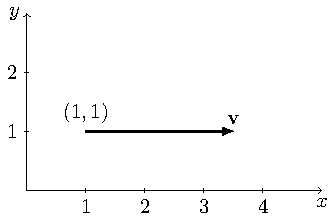
\includegraphics{vectorBaseAtPointOfAction}
\caption{سمتیہ}
\label{شکل_سمتیہ_دم_پر_عمل_درآمد_ہوتی_ہے}
\end{figure}
\end{comment}
\begin{figure}
\centering
\begin{tikzpicture}
\draw[<->] (0,3)--(0,0)--(5,0);
\draw[thick, -latex] (1,1)node[above]{$(1,1)$}--(3.5,1);
\node[above] at (3.5,1) {$\bf{v}$};
\node[left] at (0,3) {$y$};
%\node at (4,2) {کیا حال ہے};
\node[below] at (5,0) {$x$};
%\draw (4,1) edge [out=90 ,in=190,<-] (5.4,2);
%
\foreach \x/\xl in {1/1,2/2,3/3,4/4}
\draw (\x,1pt) --(\x,-1pt) node [anchor=north] {$\xl$};
\foreach \y in {1,2}
\draw (1pt,\y) --(-1pt,\y) node [anchor=east] {$\y$};
\end{tikzpicture}
\caption{سمتیہ}
\label{شکل_سمتیہ_دم_پر_عمل_درآمد_ہوتی_ہے}
\end{figure}

\حصہ{سمتی الجبرا}
دو سمتیوں کا ترسیمی  مجموعہ حاصل کرنے کی خاطر ایک سمتیہ کے سر کو دوسرے سمتیہ کی دُم  کے ساتھ ملایا جاتا ہے۔پہلی سمتیہ کی دُم سے دوسرے سمتیہ کے سر تک سمتیہ حاصل جمع ہو گا۔اس عمل کو شکل \حوالہ{شکل_سمتیہ_سمتیوں_کا_مجموعہ}-الف میں دکھایا گیا ہے۔شکل میں \سمتیہ{A} کے سر کے ساتھ \سمتیہ{B} کی دُم ملائی گئی ہے۔دو سے زیادہ سمتیوں کا مجموعہ بھی اسی عمل کو استعمال کرتے  ہوئے حاصل کیا جاتا ہے۔اس اصول کو \اصطلاح{سر سے دُم جوڑنے}\فرہنگ{اصول!سر سے دُم جوڑنا}\فرہنگ{head to tail rule}\حاشیہب{head to tail rule} کا اصول کہتے ہیں۔شکل \حوالہ{شکل_سمتیہ_سمتیوں_کا_مجموعہ}-ب میں دو سمتیوں کے دُم ملا کر ان کا مجموعہ \اصطلاح{قانون متوازی الاضلاع}\فرہنگ{قانون!متوازی الاضلاع} سے حاصل کرنا دکھایا گیا ہے جسے دیکھ کر صاف ظاہر ہے کہ $\bf{A}+\bf{B}=\bf{B}+\bf{A}$ ہے یعنی سمتیوں کا مجموعہ قانون تبادل\فرہنگ{قانون تبادل}\حاشیہب{commutative law}\فرہنگ{commutative law} پر پورا اترتا ہے۔اسی طرح سمتیوں کا مجموعہ قانون تلازمی\فرہنگ{قانون تلازمی}\حاشیہب{associative law}\فرہنگ{associative law} کے استعمال سے درج ذیل طریقے سے لکھا جا سکتا ہے۔
\begin{align}
\bf{A}+\left(\bf{B}+\bf{C}\right)=\left(\bf{A}+\bf{B}\right)+\bf{C}
\end{align}
\begin{comment}
\begin{figure}
\centering
\begin{subfigure}{0.5\textwidth}
\centering
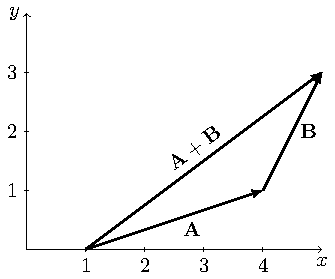
\includegraphics{figVectorHeadToTailRule}
\caption{سر کے ساتھ دُم جوڑ کر مجموعہ حاصل کیا جاتا ہے۔}
%\label{شکل_سمتیہ_سر_دم_جوڑنا}
\end{subfigure}%
%
\begin{subfigure}{0.5\textwidth}
\centering
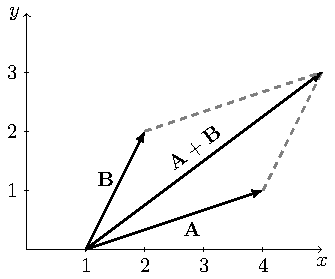
\includegraphics{figVectorParallelogramAdditionLaw}
\caption{متوازی الاضلاع سے بھی مجموعہ حاصل کیا جاتا ہے۔}
%\label{شکل_سمتیہ_متوازی_الاضلاع}
\end{subfigure}%
\caption{سمتیوں کے مجموعے کا حصول}
\label{شکل_سمتیہ_سمتیوں_کا_مجموعہ}
\end{figure}
\end{comment}

\begin{figure}
\centering
\begin{subfigure}{0.5\textwidth}
\centering
\begin{tikzpicture}
\draw[<->] (0,4)--(0,0)--(5,0);
\node[left] at (0,4) {$y$};
\node[below] at (5,0) {$x$};
\draw[thick, -latex] (1,0)--(4,1) node[pos=0.6,below]{$\bf{A}$};
\draw[thick, -latex] (4,1)--(5,3)node[pos=0.5,right]{$\bf{B}$};;
\draw[thick, -latex] (1,0)--(5,3) node[pos=0.5,sloped, above]{$\bf{A+B}$} ;
%
\foreach \x/\xl in {1/1,2/2,3/3,4/4}
\draw (\x,1pt) --(\x,-1pt) node [anchor=north] {$\xl$};
\foreach \y in {1,2,3}
\draw (+1pt,\y) --(-1pt,\y) node [anchor=east] {$\y$};
\end{tikzpicture}
\caption{سر کے ساتھ دُم جوڑ کر مجموعہ حاصل کیا جاتا ہے۔}
%\label{شکل_سمتیہ_سر_دم_جوڑنا}
\end{subfigure}%
\begin{subfigure}{0.5\textwidth}
\centering
\begin{tikzpicture}
\draw[<->] (0,4)--(0,0)--(5,0);
\node[left] at (0,4) {$y$};
\node[below] at (5,0) {$x$};
\draw[thick, -latex] (1,0)--(4,1) node[pos=0.6,below]{$\bf{A}$};
\draw[thick, dashed,gray] (4,1)--(5,3);
\draw[thick, -latex] (1,0)--(5,3) node[pos=0.5,sloped, above]{$\bf{A+B}$} ;
%\node[rotate=37] at (3,1.8){$\bf{A+B}$};
%
\draw[thick,-latex] (1,0)--(2,2) node[pos=0.6,left]{$\bf{B}$};
\draw[thick,dashed,gray](2,2)--(5,3);
%
\foreach \x/\xl in {1,2,3,4}
\draw (\x,1pt) --(\x,-1pt) node [anchor=north] {$\xl$};
\foreach \y in {1,2,3}
\draw (1pt,\y) --(-1pt,\y) node [anchor=east] {$\y$};
\end{tikzpicture}
\caption{متوازی الاضلاع سے بھی مجموعہ حاصل کیا جاتا ہے۔}
%\label{شکل_سمتیہ_متوازی_الاضلاع}
\end{subfigure}%
\caption{سمتیوں کے مجموعے کا حصول}
\label{شکل_سمتیہ_سمتیوں_کا_مجموعہ}
\end{figure}
سمتیوں کے تفریق کا اصول  جمع کے اصول سے حاصل کیا جا سکتا ہے۔ہم $\bf{A}-\bf{B}$ کو $\bf{A}+\left(-\bf{B}\right)$ لکھ سکتے ہیں جہاں $-\bf{B}$ سے مراد یہ ہے کہ سمتیہ $\bf{B}$ کی سمت الٹی کر دی گئی ہے۔یوں $\bf{A}-\bf{B}$ حاصل کرنے کی خاطر $\bf{B}$ کی سمت الٹی کرتے ہوئے اس نئے سمتیہ کو $\bf{A}$ کے ساتھ جمع کیا جاتا ہے۔

سمتیہ \سمتیہ{A} کو مثبت  غیر سمتی مقدار \عددیء{k} سے ضرب دینے سے سمتیہ کی سمت پر کوئی اثر نہیں ہوتا جبکہ اس کی لمبائی \عددیء{k} گنا ہو جاتی ہے۔اس کے برعکس سمتیہ \سمتیہ{A} کو منفی غیر سمتی مقدار \عددیء{-k} سے ضرب دینے سے سمتیہ کی سمت الٹ ہو جاتی ہے اور اس کی لمبائی \عددیء{\abs{k}} گنا ہو جاتی ہے۔

دو سمتیے اُس صورت میں برابر ہوتے ہیں جب ان کا تفریق صفر کے برابر ہو یعنی \عددیء{\kvec{A}=\kvec{B}} تب ہو گا جب \عددیء{\kvec{A}-\kvec{B}=0} ہو۔

سمتی میدان کے متغیرات کو ہم آپس میں جمع یا منفی صرف اُس صورت کریں گے جب یہ متغیرات ایک ہی نقطے پر بیان کئے گئے ہوں۔یوں کسی بھی نقطے پر دو یا دو سے زیادہ مقناطیسوں کا مجموعی مقناطیسی میدان حاصل کرتے ہوئے اس نقطے پر تمام مقناطیسوں کا علیحدہ علیحدہ مقناطیسی میدان لیتے ہوئے ان کا مجموعہ لیا جائے گا۔

اگر سمتی میدان کی بات نہ ہو رہی ہو تب مختلف مقامات پر پائے جانے والے سمتیوں کا بھی مجموعہ یا فرق لیا جا سکتا ہے۔یوں سمندر کے پانی میں ڈوبے ہوئے آب دوز کی بالائی اور نچلی سطح پر قوتوں کا مجموعہ حاصل کرتے ہوئے ہم یہ معلوم کر سکتے ہیں کہ آیا یہ مزید ڈوبے گا یا نہیں۔  

\حصہ{کارتیسی محدد}\شناخت{حصہ_سمتیہ_کارتیسی_محدد}
ایسا طریقہ جس سے کسی نقطے کا مقام بیان کیا جائے محدد\فرہنگ{محدد}\حاشیہب{coordinates}\فرہنگ{coordinates} کہلاتا ہے۔سیدھی سطح پر کسی بھی نقطے کو دو محدد سے ظاہر کیا جا سکتا ہے۔خلاء تین طرفہ\حاشیہب{three dimensional} ہے لہٰذا خلاء میں کسی بھی نقطے کو تین محدد سے ظاہر کیا جا سکتا ہے۔شکل \حوالہ{شکل_سمتیہ_اکائی_سے_سمتیہ_کا_اظہار}-الف میں دو طرفہ  \اصطلاح{کارتیسی} محدد پر اکائی لمبائی کے دو سمتیات \عددیء{\ax} اور \عددیء{\ay} دکھائے گئے ہیں۔اکائی سمتیہ \عددیء{\ax} کی سمت مثبت \عددیء{x} جانب کو ہے جبکہ \عددیء{\ay}  کی سمت مثبت \عددیء{y} جانب کو ہے۔شکل-ب میں \سمتیہ{A} دکھایا گیا ہے۔کسی بھی سمتیہ کو دو یا دو سے زیادہ سمتیوں کے مجموعے کی شکل میں لکھا جا سکتا ہے۔شکل میں \عددیء{\kvec{A}} کو \عددیء{\kvec{A}_x} اور \عددیء{\kvec{A}_y} کے مجموعے کی شکل میں دکھایا گیا ہے یعنی
\begin{align}
\kvec{A}=\kvec{A}_x+\kvec{A}_y
\end{align}

\begin{figure}
\centering
\begin{subfigure}{0.5\textwidth}
\centering
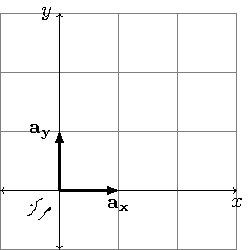
\includegraphics{unitVectorsInTwoDimensionalCartesianSpace}
\caption{اکائی سمتیہ}
%\label{شکل_سمتیہ_سر_دم_جوڑنا}
\end{subfigure}%
%
\begin{subfigure}{0.5\textwidth}
\centering
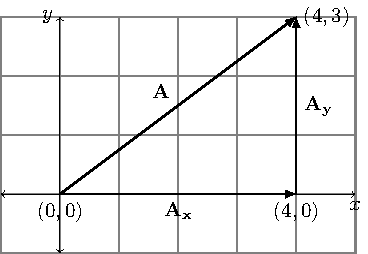
\includegraphics[scale=0.95]{vectorsRepresentationCartesianSpace}
\caption{اکائی سمتیات سے عمومی سمتیہ کا اظہار۔}
%\label{شکل_سمتیہ_متوازی_الاضلاع}
\end{subfigure}%
\caption{اکائی سمتیات اور ان کا استعمال}
\label{شکل_سمتیہ_اکائی_سے_سمتیہ_کا_اظہار}
\end{figure}
%


زمین کی سطح کو لامحدود سیدھی سطح تصور کرتے ہوئے،  اس کے \اصطلاح{ہم سطحی}\فرہنگ{ہم سطحی}\حاشیہب{coplanar}\فرہنگ{coplanar} دو عمودی لکیریں کھینچتے ہوئے ایک لکیر کو \عددیء{x} محدد اور دوسری لکیر کو \عددیء{y} محدد تصور کیا جا سکتا ہے۔زمین کے ہم سطحی لکیر سے مراد ایسی لکیر ہے جس پر ہر نقطہ اس سطح کو چھوتا ہے۔\عددیء{x} محدد کے مثبت حصے  سے گھڑی کی گردش کی الٹ سمت گھومتے ہوئے نوے درجے پر \عددیء{y} محدد کا مثبت حصہ رکھتے ہوئے اونچائی کو \عددیء{z} محدد کے مثبت حصے  سے ظاہر کیا جائے گا۔ اب اگر اونچائی صفر رکھتے ہوئے \عددیء{x} اور \عددیء{y} کو تبدیل کیا جائے تو ہم زمین کی سطح پر حرکت کریں گے۔اس طرح ہم دیکھتے ہیں کہ زمین کی سطح پر \عددیء{z=0} جبکہ اس پر \عددیء{x} اور \عددیء{y} آزاد متغیرات ہیں۔یوں زمین کی سطح کو \عددیء{z=0} سطح کہتے ہیں جسے
\begin{align*}
z=0, \quad  x\le \abs{\mp \infty}, \quad y \le \abs{\mp \infty}
\end{align*} 
لکھا جا سکتا ہے۔  شکل \حوالہ{شکل_سمتیہ_کارتیسی_نقطہ_اور_عمودی_سطحیں}-الف میں اس سطح کی نشاندہی کی گئی ہے۔اسی شکل میں \عددیء{y=0} سطح اور \عددیء{x=0} سطح کی بھی نشاندہی کی گئی ہے۔

\begin{figure}
\centering
\begin{subfigure}{0.5\textwidth}
\centering
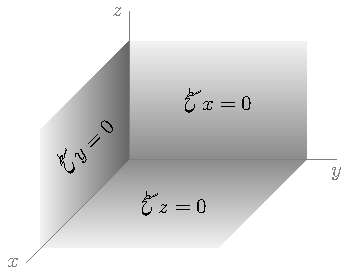
\includegraphics{figVectorPlaneSurfacesCartesian}
\caption{کارتیسی محدد میں عمودی سیدھی سطحیں۔}
\label{شکل_سمتیہ_کارتیسی_عمودی-تین_سطحیں}
\end{subfigure}%
%
\begin{subfigure}{0.5\textwidth}
\centering
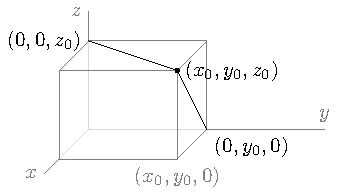
\includegraphics{figVectorPerpendicularsFromPointToCartesianAxis3D}
\caption{نقطے سے محدد پر عمود۔}
\label{شکل_سمتیہ_نقطے_سے_کارتیسی_محدد_پر_عمود}
\end{subfigure}%
\caption{کارتیسی نظام میں نقطہ اور تین عمودی سطحیں۔}
\label{شکل_سمتیہ_کارتیسی_نقطہ_اور_عمودی_سطحیں}
\end{figure}
شکل  \حوالہ{شکل_سمتیہ_کارتیسی_نقطہ_اور_عمودی_سطحیں}-ب  کو دیکھئیے۔ کارتیسی محدد میں کسی بھی نقطے کو \عددیء{(x_0,y_0,z_0)} لکھا جا سکتا ہے۔اس نقطے تک پہنچنے کی خاطر  کارتیسی محدد کے مرکز سے پہلے \عددیء{x} محدد کے متوازی \عددیء{x_0}  فاصلہ طے کرتے ہوئے \عددیء{(x_0,0,0)} تک پہنچیں۔اس کے بعد \عددیء{y} محدد کے متوازی \عددیء{y_0} فاصلہ طے کرتے ہوئے \عددیء{(x_0,y_0,0)} تک پہنچیں  اور آخرکار \عددیء{z} محدد کے متوازی \عددیء{z_0} فاصلہ طے کرتے ہوئے درکار نقطہ \عددیء{(x_0,y_0,z_0)} تک پہنچیں۔اس عمل میں یہ ضروری نہیں کہ پہلے \عددیء{x} محدد کے متوازی ہی چلا جائے۔آپ مرکز سے پہلے \عددیء{y} محدد کے متوازی \عددیء{y_0} فاصلہ طے کرنے کے بعد \عددیء{z} محدد کے متوازی \عددیء{z_0} اور آخرکار \عددیء{x} محدد کے متوازی \عددیء{x_0} فاصلہ طے کرتے ہوئے بھی اسی نقطے تک پہنچ سکتے ہیں۔تینوں فاصلوں کو کسی بھی ترتیب سے طے کیا جا سکتا ہے۔

 نقطہ \عددیء{(x_0,y_0,z_0)} سے \عددیء{x} محدد پر عمود بناتے ہوئے نقطہ  \عددیء{(x_0,0,0)} حاصل ہوتا ہے۔اسی طرح اسی نقطے سے \عددیء{y} محدد پر عمود بناتے ہوئے نقطہ  \عددیء{(0,y_0,0)} اور \عددیء{z} محدد پر عمود بناتے ہوئے نقطہ \عددیء{(0,0,z_0)} حاصل ہوتا ہے۔نقطہ \عددیء{(x_0,y_0,z_0)} سے \عددیء{y} محدد اور \عددیء{z} محدد پر عمودی لکیریں گہری سیاہی سے دکھائی گئی ہیں جبکہ شکل کو صاف ستھرا رکھنے کی خاطر \عددی{(x_0,y_0,z_0)} سے \عددی{x} محدد پر عمودی لکیر نہیں دکھائی گئی۔ اگر \عددیء{(x_0,y_0,z_0)} سے  شروع ہوتے ہوئے \عددیء{z} محدد کے متوازی یوں چلا جائے کہ آخرکار \عددیء{z=0} ہو جائے تو نقطہ \عددیء{(x_0,y_0,0)} حاصل ہو گا۔ اب اگر نقطہ \عددیء{(x_0,y_0,0)} سے \عددیء{x} محدد کے متوازی یوں چلا جائے کہ آخرکار \عددیء{x=0} ہو جائے تو نقطہ \عددیء{(0,y_0,0)} حاصل ہو گا۔یہ وہی نقطہ ہے جو \عددیء{(x_0,y_0,z_0)} سے \عددیء{y} محدد پر عمودی لکیر بناتے ہوئے حاصل ہوتا ہے۔اس عمل میں ہم پہلے \عددیء{x} محدد کے متوازی چلتے ہوئے \عددیء{x=0} کرنے کے بعد \عددیء{z} محدد کے متوازی چلتے ہوئے \عددیء{z=0} کرتے ہوئے بھی نقطہ \عددیء{(0,y_0,0)} تک پہنچ سکتے تھے۔

نقطہ \عددیء{(x_0,y_0,z_0)} تک قدر مختلف انداز سے بھی پہنچا جا سکتا ہے جسے کارتیسی محدد میں سمجھنا زیادہ آسان ہے۔شکل \حوالہ{شکل_سمتیہ_تین_عمودی_سطحوں_سے_نقطہ} کو دیکھئیے۔فرض کریں کہ \عددیء{x=x_0} پر لامحدود وسعت کی \عددیء{yz} سیدھی سطح بنائی جائے۔ایسی سطح کو \عددیء{x=x_0} سطح  کہتے ہیں۔اس سطح کو
\begin{align*}
x=x_0, \quad  y\le \abs{\mp \infty}, \quad z \le \abs{\mp \infty}
\end{align*} 
لکھا جا سکتا ہے۔اس مساوات میں \عددیء{x_0} مستقل ہے جبکہ \عددیء{y} اور \عددیء{z} متغیرات ہیں۔دو متغیرات کی مساوات سطح کو ظاہر کرتی ہے۔اگر \عددیء{y=y_0} پر لامحدود وسعت کی \عددیء{xz} سیدھی سطح بنائی جائے تو یہ دو سطحیں  آپس میں سیدھی لکیر پر ملیں گی۔یہ لکیر
\begin{align*}
x=x_0, \quad  y=y_0, \quad z \le \abs{\mp \infty}
\end{align*} 
لکھی جا سکتی ہے۔اس مساوات میں \عددیء{x_0} اور \عددیء{y_0} مستقل ہیں جبکہ \عددیء{z} متغیر ہے۔ایک متغیر کی مساوات لکیر کو ظاہر کرتی ہے۔اب اگر \عددیء{z=z_0} پر لامحدود \عددیء{xy} سیدھی سطح بھی بنائی جائے تب یہ تینوں سطحے ایک نقطے \عددیء{N(x_0,y_0,z_0)} پر ایک دونوں کو چھوئنگے۔شکل \حوالہ{شکل_سمتیہ_تین_عمودی_سطحوں_سے_نقطہ} میں  لامحدود سطحوں کے کچھ حصے دکھائے گئے ہیں۔آپ دیکھیں گے کہ نقطے تک پہنچنے کا یہ طریقہ دیگر محدد میں استعمال کرنا لازمی ثابت ہو گا۔
\begin{figure}
\centering
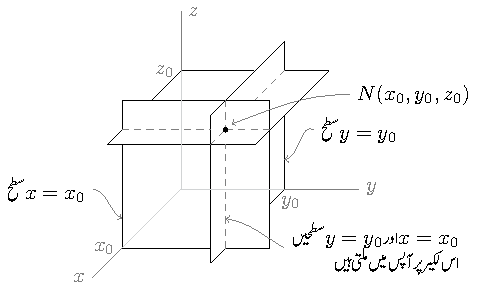
\includegraphics{figVectorLineAsSurfacesTouching}
\caption{تین عمودی سطحوں سے نقطے کا حصول۔}
\label{شکل_سمتیہ_تین_عمودی_سطحوں_سے_نقطہ}
\end{figure}

اگر سطح \عددیء{x=x_0}  کے متوازی \عددیء{x=x_0+\dif x} پر اور اسی طرح \عددیء{y=y_0} کے متوازی \عددیء{y=y_0+\dif y} اور \عددیء{z=z_0} کے متوازی \عددیء{z=z_0+\dif z} سطحیں رکھے جائیں تو یہ چھ سطحے ایک چھوٹی  مکعب نما حجم  کو گھیریں گی جسے شکل \حوالہ{شکل_سمتیہ_کارتیسی_چھوٹی_مکعب} میں دکھایا گیا ہے جبکہ یہ تین نئی سطحیں آپس میں نقطہ \عددیء{N'} پر ملیں گی ۔
\begin{figure}
\centering
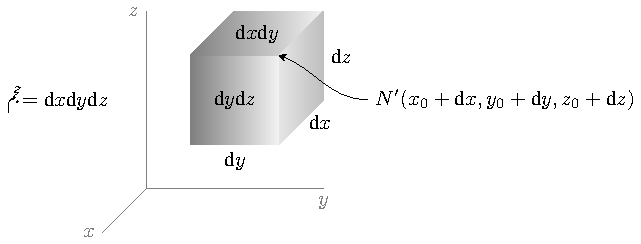
\includegraphics{figVectorCubeShaded}
\caption{چھ سطحے مکعب گھیرتی ہیں۔}
\label{شکل_سمتیہ_کارتیسی_چھوٹی_مکعب}
\end{figure}
اس مکعب نما کے اطراف \عددیء{\dif x}، \عددیء{\dif y} اور \عددیء{\dif z} ہیں۔ اس کی اوپر والی سطح کا رقبہ \عددیء{\dif x \dif y} ہے۔اسی طرح اس کی نچلی سطح کا رقبہ بھی \عددیء{\dif x \dif y} ہے۔سامنے سطح  اور پچھلی سطح دونوں \عددیء{\dif y \dif z} رقبے رکھتے ہیں جبکہ بائیں  اور دائیں سطحوں کے رقبے \عددیء{\dif x \dif z} کے برابر ہیں۔اس مکعب نما کی حجم \عددیء{\dif x \dif y \dif z} ہے۔نقطہ \عددیء{N'(x_0+\dif x,y_0+\dif y,z_0+\dif z)} شکل میں دکھایا گیا ہے جبکہ
 نقطہ \عددیء{N(x_0,y_0 ,z_0)} مکعب نما کا وہ واحد کونا ہے جسے شکل میں نہیں دکھایا گیا۔ان دو نقطوں کے درمیان فاصلہ \عددیء{NN'=\sqrt{\dif x^2+\dif y^2+\dif z^2}} ہے۔ 

کارتیسی محدد کے تینوں متغیرات تبدیل کرنے سے ہم \عددیء{N} سے \عددیء{N'} پہنچتے ہیں۔\عددیء{N} سے \عددیء{N'} تک کی سمتیہ

\begin{align}\label{مساوات_سمتیہ_کارتیسی_چھوٹا_فاصلہ}
\dif \kvec{L}=\dif x \ax+\dif y \ay+\dif z \az
\end{align}
لکھی جاتی ہے۔یہ مساوات کسی بھی دو قریبی نقطوں کے درمیان سمتی لمبائی دیتی ہے۔
%==================
\حصہ{اکائی سمتیات}
حصہ  \حوالہ{حصہ_سمتیہ_کارتیسی_محدد} کے شروع میں دو طرفہ کارتیسی نظام  میں سیدھی سطح پر کسی بھی سمتیہ کو دو سمتیات کی صورت میں لکھنا دکھایا گیا۔یہی طریقہ تین طرفہ کارتیسی نظام کے لئے بھی استعمال کیا جاتا ہے۔ تین طرفہ کارتیسی نظام کے تین اکائی سمتیات \عددیء{\ax}، \عددیء{\ay} اور \عددیء{\az} لکھے جاتے ہیں۔یہ تینوں سمتیات آپس میں عمودی ہیں۔کسی بھی اکائی سمتیہ کی طرح یہ تین اکائی سمتیات اکائی لمبائی رکھتے ہیں۔ \عددیء{\ax} کی سمت \عددیء{x} محدد کے بڑھتے جانب کو ہے۔اسی طرح \عددیء{\ay} کی سمت \عددیء{y} محدد کے بڑھتے جانب کو اور \عددیء{\az} کی سمت \عددیء{z} محدد کے بڑھتے جانب کو ہے۔شکل \حوالہ{شکل_سمتیہ_کارتیسی_تین_اکائی_سمتیات}-الف میں یہ تینوں اکائی سمتیات دکھائے گئے ہیں۔اسی شکل میں نقطہ \عددیء{(0,1,2)} پر سمتیہ دکھایا گیا ہے جس کی لمبائی دو کے برابر ہے جبکہ یہ اکائی سمتیہ \عددیء{\ay} کی سمت میں ہے۔اس سمتیہ کو \عددیء{2\ay} لکھا جا سکتا ہے۔یاد رہے کہ ایسے دو سمتیات برابر ہوتے ہیں جن کا طول برابر ہو اور جو ایک ہی سمت میں ہوں۔ یوں سمت تبدیل کئے بغیر سمتیہ کو کارتیسی محدد کے مرکز منتقل کرتے ہوئے اس کی قیمت نسبتاً آسانی سے لکھی جا سکتی ہے۔
\begin{figure}
\centering
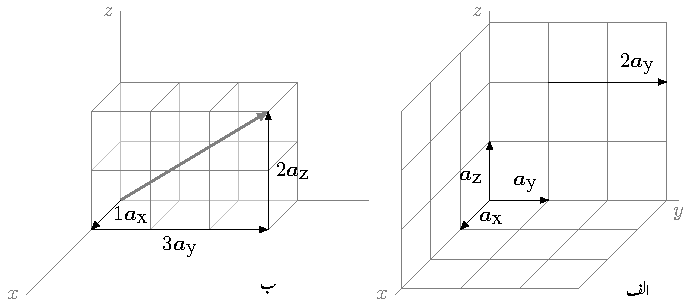
\includegraphics{figVector3DUnitVectors}
\caption{کارتیسی نظام کے اکائی سمتیات اور ان کا استعمال}
\label{شکل_سمتیہ_کارتیسی_تین_اکائی_سمتیات}
\end{figure}
%
\begin{figure}
\centering
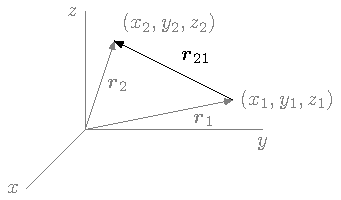
\includegraphics{figVector3DcartesianVectorEquation}
\caption{کارتیسی نظام میں سمتیہ کی مساوات کا حصول}
\label{شکل_سمتیہ_کارتیسی_سمتیہ_کی_مساوات}
\end{figure}
%
\begin{figure}
\centering
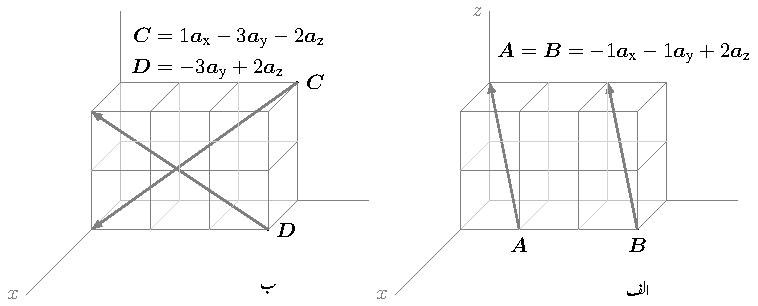
\includegraphics[width=\textwidth]{figVector3DcartesianVectors}
\caption{کارتیسی نظام میں چند سمتیات۔}
\label{شکل_سمتیہ_کارتیسی_چند_سمتیات}
\end{figure}
%

شکل \حوالہ{شکل_سمتیہ_کارتیسی_سمتیہ_کی_مساوات} میں  مرکز سے \عددیء{(x_1,y_1,z_1)} تک سمتیہ \عددیء{\kvec{r}_1=x_1 \ax+y_1\ay+z_1\az} اور  مرکز سے \عددیء{(x_2,y_2,z_2)} تک سمتیہ \عددیء{\kvec{r}_2=x_2 \ax+y_2\ay+z_2\az} دکھائے گئے ہیں۔شکل میں سمتیہ \عددیء{\kvec{r}_{21}} بھی دکھائی گئی ہے جس کی دُم  \عددیء{(x_1,y_1,z_1)} اور  نوک \عددیء{(x_2,y_2,z_2)} پر ہے۔ سر سے دُم جوڑنے کے اصول کے استعمال سے \عددیء{\kvec{r}_2=\kvec{r}_{21}+\kvec{r}_1} لکھا جا سکتا ہے جس سے 
\begin{gather}
\begin{aligned}\label{مساوات_سمتیہ_کارتیسی_نظام_میں_قیمت}
\kvec{r}_{21}&=\kvec{r}_2-\kvec{r}_1\\
&=(x_2-x_1) \ax+(y_2-y_1)\ay+(z_2-z_1)\az
\end{aligned}
\end{gather}
حاصل ہوتا ہے۔اس مساوات کے استعمال سے سمتیہ کی مساوات باآسانی حاصل ہوتی ہے۔سمتیہ \عددیء{\kvec{r}_{21}} لکھتے ہوئے زیرنوشت میں سمتیہ کی نوک کو \عددیء{2} اور اس کی دُم  کو \عددیء{1} سے ظاہر کیا گیا ہے۔اس کتاب میں سمتیہ لکھتے ہوئے نوک اور دُم  کو اسی ترتیب سے زیرنوشت میں لکھا جائے گا۔یوں سمتیہ \عددیء{\kvec{r}_{21}} کو تین اجزاء \عددیء{(x_2-x_1)\ax}، \عددیء{(y_2-y_1)\ay} اور \عددیء{(z_2-z_1)\az} کے  مجموعے کی شکل میں لکھا جا سکتا ہے۔

شکل \حوالہ{شکل_سمتیہ_کارتیسی_تین_اکائی_سمتیات}-ب میں مرکز سے \عددیء{(1,3,2)} تک سمتیہ دکھایا گیا ہے۔آپ دیکھ سکتے ہیں کہ اس کو تین سمتیات کا مجموعہ لکھا جا سکتا ہے یعنی \عددیء{1\ax+3\ay+2\az} جہاں اکائی سمتیات استعمال کرتے ہوئے تینوں اجزاء کو لکھا گیا ہے۔ سمتیہ کی دُم \عددیء{(0,0,0)} اور اس کی نوک \عددیء{(1,3,2)} پر لیتے ہوئے  یہی جواب  مساوات \حوالہ{مساوات_سمتیہ_کارتیسی_نظام_میں_قیمت} سے بھی حاصل ہوتا ہے۔

شکل \حوالہ{شکل_سمتیہ_کارتیسی_چند_سمتیات}-الف میں دو متوازی سمتیات \عددیء{\kvec{A}} اور \عددیء{\kvec{B}} دکھائے ہیں جن کی لمبائی برابر ہے۔ چونکہ ان کی لمبائی برابر ہے اور یہ دونوں ایک ہی سمت میں ہیں لہٰذا \عددیء{\kvec{A}=\kvec{B}=-1\ax-1\ay+2\az} لکھا جائے گا۔شکل \حوالہ{شکل_سمتیہ_کارتیسی_چند_سمتیات}-ب میں \عددیء{\kvec{C}} کی دُم سے \عددیء{\ax} جانب ایک قدم اور یہاں سے \عددیء{-\ay} جانب تین قدم اور آخرکار \عددیء{-\az} جانب دو قدم چلنے سے اس کی نوک تک پہنچا جا سکتا ہے لہٰذا \عددیء{\kvec{C}=1\ax-3\ay-2\az} لکھا جائے گا۔ اسی طرح \عددیء{\kvec{D}} کی دُم سے  \عددیء{-\ay} جانب تین قدم اور پھر \عددیء{\az} جانب دو قدم چلتے ہوئےسمتیہ کی نوک تک پہنچا جایا سکتا ہے لہٰذا \عددیء{\kvec{D}=-3\ay+2\az} لکھا جائے گا۔سمتیہ \عددیء{\kvec{D}} کو دو اجزاء کی شکل میں لکھا گیا ہے چونکہ اس کے تیسرے جزو کی لمبائی صفر کے برابر ہے۔
%=====================
\ابتدا{مشق}
مساوات \حوالہ{مساوات_سمتیہ_کارتیسی_نظام_میں_قیمت} کے استعمال سے شکل \حوالہ{شکل_سمتیہ_کارتیسی_چند_سمتیات} میں تمام سمتیات لکھیں۔

جوابات:تمام جوابات شکل میں دئے گئے ہیں۔
\انتہا{مشق}
%======================
\begin{figure}
\centering
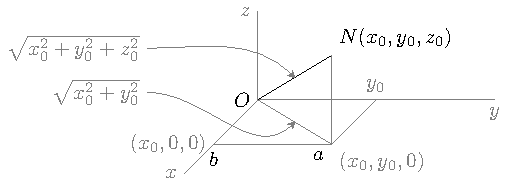
\includegraphics{figVectorCartesianAmplitudeFromPythagorousTheorem}
\caption{کارتیسی نظام میں سمتیہ کا طول۔}
\label{شکل_سمتیہ_کارتیسی_سمتیہ_طول}
\end{figure}

شکل \حوالہ{شکل_سمتیہ_کارتیسی_سمتیہ_طول} میں مرکز سے نقطہ \عددیء{N(x_0,y_0,z_0)} تک کا فاصلہ \عددیء{ON} مسئلہ \اصطلاح{فیثاغورث}\فرہنگ{فیثاغورث}\حاشیہب{Pythagoras theorem}\فرہنگ{Pythagoras theorem} سے حاصل کیا جا سکتا ہے۔اس نقطے سے \عددیء{z=0} سطح پر عمود سے نقطہ \عددیء{a} حاصل ہوتا ہے۔نقطہ \عددیء{a} سے \عددیء{x} محدد پر عمود نقطہ \عددیء{b} دیتا ہے۔تکون \عددیء{Oba} میں \عددیء{O} سے \عددیء{b} کا فاصلہ \عددیء{x_0} ہے جبکہ \عددیء{b} سے \عددیء{a} کا فاصلہ \عددیء{y_0} ہے۔یوں فاصلہ \عددیء{Oa} مسئلہ فیثاغورث کی مدد سے  \عددیء{\sqrt{x_0^2+y_0^2}} کے برابر ہو گا۔ تکون \عددیء{OaN} میں \عددیء{a} پر \عددیء{90^{\circ}} کا زاویہ پایا جاتا ہے۔یوں مسئلہ فیثاغورث کی مدد سے \عددیء{ON} کا فاصلہ \عددیء{\sqrt{x_0^2+y_0^2+z_0^2}} حاصل ہوتا ہے۔

مساوات \حوالہ{مساوات_سمتیہ_کارتیسی_نظام_میں_قیمت} سمتیہ کی عمومی مساوات ہے۔اس میں دئے سمتیہ \عددیء{\kvec{r}_{21}} کی دُم محدد کے مرکز پر رکھنے سے صاف ظاہر ہے کہ سمتیہ کی مقدار
\begin{align}
\abs{\kvec{r}_{21}}=r_{21}=\sqrt{(x_2-x_1)^2+(y_2-y_1)^2+(z_2-z_1)^2}
\end{align}
کے برابر ہے۔اگر سمتیہ کو اس کی مقدار سے تقسیم کیا جائے تو حاصل جواب کی مقدار اکائی ہو گی جبکہ اس کی سمت میں کوئی تبدیلی رونما نہیں ہو گی۔یوں  \عددیء{\kvec{r}_{21}} کو \عددیء{\abs{\kvec{r}_{21}}} سے تقسیم کرتے ہوئے \عددیء{\kvec{r}_{21}} کی سمت میں اکائی سمتیہ \عددیء{\kvec{a}_{r21}} حاصل کی جا سکتی ہے۔
\begin{align}
\kvec{a}_{r21}=\frac{\kvec{r}_{21}}{\abs{\kvec{r}_{21}}}=\frac{(x_2-x_1) \ax+(y_2-y_1)\ay+(z_2-z_1)\az}{\sqrt{(x_2-x_1)^2+(y_2-y_1)^2+(z_2-z_1)^2}}
\end{align}
یاد رہے کہ سمتیہ کی سمت اور طول تبدیل کئے بغیر اسے ایک مقام سے دوسری مقام منتقل کیا جا سکتا ہے۔البتہ وہ سمتیہ جو کسی نقطے کی مقام تعین کرتا ہو کو اگر کہیں اور منتقل کیا جائے تو ایسی صورت میں  سمتیہ کی نوک درکار نقطے پر نہیں رہے گی۔اسی حقیقت کی بنا پر میدان ظاہر کرنے والے سمتیہ کو اپنی جگہ سے نہیں ہٹایا جا سکتا۔میدانی سمتیہ کی دُم اس مقام پر پائی جاتی ہے جہاں میدان بیان کی جا رہی ہو۔  

سمتیات کے استعمال سے نقطہ \عددیء{(x,y,z)} کے مقام کو \عددیء{\kvec{r}=x\ax+y\ay+z\az} لکھا جاتا ہے۔کسی بھی سمتیہ مثلاً قوت \عددیء{\kvec{F}} کو بالکل اسی طرح  \عددیء{{\kvec{F}=F_x\ax+F_y\ay+F_z\az}} لکھا جاتا ہے جہاں \عددیء{F_x \ax}، \عددیء{F_y \ay} اور \عددیء{F_z\az} اس کے تین اجزاء اور
  \عددیء{\abs{\kvec{F}}=\sqrt{F_x^2+F_y^2+F_z^2}} قوت کی مقدار ہے۔
%======================
\ابتدا{مثال}
نقطہ \عددیء{(-5,2,-1)}  کا مقام ظاہر کرنے والا سمتیہ اور اس سمتیہ کا طول حاصل کریں۔اسی سمتیہ کی سمت میں اکائی سمتیہ حاصل کریں۔

حل:مرکز سے اس نقطے تک کا سمتیہ
\begin{align*}
\kvec{r}=-5\ax+2\ay-1\az
\end{align*}
ہے جبکہ اس سمتیہ  کا طول
\begin{align*}
\abs{\kvec{r}}=\sqrt{5^2+2^2+1^1}=\sqrt{30}
\end{align*}
 ہے۔یوں اکائی سمتیہ درج ذیل ہو گا۔
\begin{align*}
\kvec{a}_r=\tfrac{-5\ax+2\ay-1\az}{\sqrt{30}}
\end{align*}
\انتہا{مثال}
%=====================

\ابتدا{مثال}\شناخت{مثال_سمتیہ_نقطے_سے_درمیان_تک_سمتیہ}
شکل \حوالہ{شکل_سمتیہ_استعمال_سمتیہ_مثال} میں تین نقطے \عددیء{M(1,6,4)}، \عددیء{N(4,5,1)} اور \عددیء{P(1,2,2)} دئے گئے ہیں۔\عددیء{M} اور \عددیء{N} کے درمیان سیدھی لکیر پر \عددیء{M} سے کل فاصلے کے  \عددیء{\tfrac{1}{3}} پر نقطہ \عددیء{Q} پایا جاتا ہے۔\عددیء{Q} سے \عددیء{P} تک سمتیہ حاصل کرتے ہوئے ان دو نقطوں کے درمیان فاصلہ معلوم کریں۔
\begin{figure}
\centering
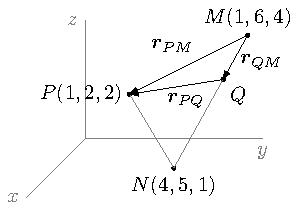
\includegraphics{figVectorExampleA}
\caption{سمتیوں کا استعمال}
\label{شکل_سمتیہ_استعمال_سمتیہ_مثال}
\end{figure}
حل:\عددیء{M} سے \عددیء{N} تک سمتیہ
\begin{align*}
\kvec{r}_{NM}&=(4-1)\ax+(5-6)\ay+(1-4)\az\\
&=3\ax-1\ay-3\az
\end{align*}
ہے۔\عددیء{M} سے \عددیء{Q} تک سمتیہ \عددیء{\kvec{r}_{QM}} اور \عددیء{\kvec{r}_{NM}} ایک ہی سمت میں ہیں جبکہ \عددیء{\abs{\kvec{r}_{QM}}=\tfrac{1}{3}\abs{\kvec{r}_{NM}}} کے برابر ہے۔یوں
\begin{align*}
\kvec{r}_{QM}=\frac{1}{3}\kvec{r}_{NM}=\frac{1}{3}(3\ax-1\ay-3\az)=1\ax-\frac{1}{3}\ay-1\az
\end{align*}
ہو گا۔\عددیء{M} سے \عددیء{P} تک سمتیہ
\begin{align*}
\kvec{r}_{PM}&=(1-1)\ax+(2-6)\ay+(2-4)\az\\
&=-4\ay-2\az
\end{align*}
ہے۔شکل کو دیکھتے ہوئے ہم لکھ سکتے ہیں \عددیء{\kvec{r}_{QM}+\kvec{r}_{PQ}=\kvec{r}_{PM}} لہٰذا
\begin{align*}
\kvec{r}_{PQ}&=\kvec{r}_{PM}-\kvec{r}_{QM}\\
&=(-4\ay-2\az)-(1\ax-\frac{1}{3}\ay-1\az)\\
&=-1\ax-\frac{11}{3}\ay-1\az
\end{align*}
ہو گا۔\عددیء{Q} سے \عددیء{P} تک فاصلہ \عددیء{\sqrt{1^1+\left(\tfrac{11}{3}\right)^2+1^2}=3.93} ہے۔
\انتہا{مثال}
%===================
\ابتدا{مشق}
مثال \حوالہ{مثال_سمتیہ_نقطے_سے_درمیان_تک_سمتیہ} میں دئے نقطوں کو استعمال کرتے ہوئے \عددیء{M} سے \عددیء{P} تک سمتیہ حاصل کریں۔اسی طرح \عددیء{P} سے \عددیء{N} تک سمتیہ اور \عددیء{M} سے \عددیء{N} تک سمتیہ حاصل کریں۔پہلے دو جوابات کو استعمال کرتے ہوئے \اصطلاح{سر سے دُم جوڑنے} کے اصول سے تیسرا سمتیہ دوبارہ حاصل کریں۔

جوابات:\عددیء{-5\ax-4\ay} ، \عددیء{-1\ax+4\ay+12\az} اور \عددیء{-6\ax+12\az}

\انتہا{مشق}
%============================================


\حصہ{سمتی رقبہ}
کسی بھی سطح کے دو اطراف ہوتے ہیں۔یوں سطح کے کسی بھی نقطے پر دو آپس میں الٹ سمتوں میں عمود بنائے جا سکتے ہیں۔سیدھی سطح جس کا رقبہ \عددیء{S} ہو کے ایک طرف پر اکائی عمود \عددیء{\kvec{a}_N} اور دوسری طرف پر اکائی عمود \عددیء{-\kvec{a}_N} بنائے جا سکتے ہیں۔اگر ان دو عمود میں سے ایک عمود مثلاً \عددیء{\kvec{a}_N} کو سطح کی سمت\حاشیہد{عمود سطح کے ساتھ نوے درجہ زاویہ بناتا ہے۔\عددیء{\kvec{a}_N} کے زیرنوشت میں \عددیء{N}، لفظ \موٹا{نوے} کے پہلے حرف کی آواز کو ظاہر کرتا ہے۔} تصور کیا جائے تب اس سطح کا \اصطلاح{سمتی رقبہ}\فرہنگ{سمتی رقبہ}\حاشیہب{vector area}\فرہنگ{vector area} \عددیء{S\kvec{a}_N} ہو گا۔بند سطح کے  بیرونی اکائی عمود کو سطح کی سمت تصور کیا جاتا ہے۔شکل \حوالہ{شکل_سمتیہ_سمتی_رقبہ} میں سمتی رقبے \عددیء{\kvec{A}_1} اور \عددیء{\kvec{A}_2} دکھائے گئے ہیں جہاں بند سطح کے بیرونی عمود کو ہی سطح کی سمت دکھایا گیا ہے۔
\begin{figure}
\centering
\includegraphics{figVectorVectorArea}
\caption{سمتی رقبہ}
\label{شکل_سمتیہ_سمتی_رقبہ}
\end{figure}


\حصہ{غیر سمتی ضرب}
دو سمتیات \عددیء{\kvec{A}} اور \عددیء{\kvec{B}} کے \اصطلاح{غیر سمتی ضرب}\فرہنگ{غیر سمتی ضرب}\فرہنگ{نقطہ ضرب}\فرہنگ{غیر سمتی ضرب}\حاشیہب{scalar product}\فرہنگ{scalar product} سے مراد \عددیء{\kvec{A}} کی مقدار ضربِ  \عددیء{\kvec{B}} کی مقدار ضربِ سمتیوں کے مابین چھوٹے زاویے کا کوسائن ہے۔غیر سمتی ضرب کا حاصل جواب غیر سمتی مقدار ہوتی ہے۔
\begin{align}\label{مساوات_سمتیہ_غیر_سمتی_ضرب}
\kvec{A} \cdot \kvec{B}=\abs{\kvec{A}} \abs{\kvec{B}} \cos \theta_{AB}
\end{align}

اگر دونوں سمتیات کی دُم ایک ہی جگہ پر نہ ہو تب ان کے مابین زاویہ دریافت کرنے کی  خاطر سمتیوں کی سمت تبدیل کئے بغیر انہیں ایک نقطے پر منتقل کیا جا سکتا ہے۔غیر سمتی ضرب دو سمتیوں کے مابین کیا جاتا ہے جبکہ اس کا حاصل جواب غیر سمتی مقدار ہوتا ہے جس کی وجہ سے اسے  \اصطلاح{غیر سمتی ضرب} بھی کہا جاتا ہے۔غیر سمتی ضرب کو سمتیوں کے درمیان نقطے سے ظاہر کیا جاتا ہے۔اسی وجہ سے اسے \اصطلاح{ضرب نقطہ}\حاشیہب{dot product}\فرہنگ{dot product} بھی کہا جاتا ہے۔ یوں \عددیء{\kvec{A} \cdot \kvec{B}} کو "\عددیء{\kvec{A}}نقطہ \عددیء{\kvec{B}}" پڑھا جاتا ہے۔بالکل سادہ ضرب کی طرح \عددیء{\kvec{A} \cdot \kvec{B}} کو \عددیء{\kvec{B} \cdot \kvec{A}} بھی لکھا جا سکتا ہے یعنی غیر سمتی ضرب میں متغیرات کی ترتیب اہمیت نہیں رکھتی۔

کارتیسی اکائی سمتیات \عددیء{\ax}، \عددیء{\ay} اور \عددیء{\az} آپس میں عمودی ہیں لہٰذا ان میں کسی بھی دو سمتیات کے درمیان \عددیء{\SI{90}{\degree}} زاویہ پایا جاتا ہے۔چونکہ \عددیء{\cos 90=0} کے برابر ہوتا ہے لہٰذا ان میں کسی بھی دو سمتیوں کا غیر سمتی ضرب صفر کے برابر ہوتا ہے یعنی
\begin{align}\label{مساوات_سمتیہ_عمودی_نقطہ_ضرب_برابر_صفر_اجزاء}
\ax \cdot \ay =0, \quad \ax \cdot \az=0, \quad \ay \cdot \az=0
\end{align}
ایک ہی سمت میں دو سمتیوں کے درمیان صفر زاویہ ہوتا ہے اور \عددیء{\cos 0=1} کے برابر ہے۔ اکائی سمتیہ کا طول بھی ایک کے برابر ہے لہٰذا مساوات \حوالہ{مساوات_سمتیہ_غیر_سمتی_ضرب} کے تحت \عددیء{\ax} اور \عددیء{\ax} کا غیر سمتی ضرب
\begin{align*}
\ax \cdot \ax=(\abs{\ax})(\abs{\ax})(\cos 0\degree)=(1)(1)(1)=1
\end{align*}
ہو گا۔بقایا دو کارتیسی اکائی سمتیات کا خود غیر سمتی ضرب بھی ایک کے برابر ہے۔
\begin{align}\label{مساوات_سمتیہ_عمودی_نقطہ_ضرب_برابر_ایک_اجزاء}
\ax \cdot \ax=1, \quad \ay \cdot \ay=1, \quad \az \cdot \az=1
\end{align}
مساوات \حوالہ{مساوات_سمتیہ_عمودی_نقطہ_ضرب_برابر_صفر_اجزاء} اور مساوات \حوالہ{مساوات_سمتیہ_عمودی_نقطہ_ضرب_برابر_ایک_اجزاء} کو \اصطلاح{کرونیکر ڈیلٹا}\فرہنگ{کرونیکر ڈیلٹا}\حاشیہد{یہ لیوپولڈ کرونیکر کے نام سے  منسوب ہے۔} \عددیء{\delta_{ij}} کی مدد سے ایک ہی مساوات کی مدد سے یوں لکھا جا سکتا ہے۔
\begin{align}
\kvec{a}_i \cdot \kvec{a}_j=\delta_{ij}
\end{align}
جہاں
\begin{align}
\delta_{ij}=
\begin{cases}
0 \quad  \quad  i\ne j \; \textup{ اگر}\\
1 \quad \quad i=j \; \textup{ اگر}
\end{cases}
\end{align}
کے برابر ہے یعنی \عددیء{i=j} کی صورت میں ہی \عددیء{\delta_{ij}} کی قیمت ایک  جبکہ \عددیء{i\ne j} کی صورت میں ہی \عددیء{\delta_{ij}} کی قیمت صفر کے برابر لی جاتی ہے۔یوں \عددیء{\ax \cdot \ay} کی صورت میں \عددیء{i=\ax} جبکہ \عددیء{j=\ay} کے برابر ہیں۔یوں \عددیء{i} اور \عددیء{j} برابر نہیں ہیں لہٰذا حاصل جواب صفر کے برابر ہو گا۔اس کے برعکس \عددیء{\az \cdot \az} کی صورت میں \عددیء{i=\az} اور \عددیء{j=\az} ہیں لہٰذا \عددیء{i=j} ہے اور یوں حاصل جواب ایک کے برابر ہے۔

کارتیسی تین عمودی اکائیوں کی مدد سے سمتیات کا غیر سمتی ضرب نہایت آسانی سے حاصل ہوتا ہے۔یوں اگر \عددیء{\kvec{A}=A_x\ax+A_y\ay+A_z\az} اور  \عددیء{\kvec{B}=B_x\ax+B_y\ay+B_z\az}  دو سمتیات ہوں تب ان کا غیر سمتی ضرب
\begin{align*}
\kvec{A} \cdot \kvec{B}&=(A_x\ax+A_y\ay+A_z\az) \cdot (B_x\ax+B_y\ay+B_z\az)\\
&=A_x B_x \ax \cdot \ax+A_x B_y \ax \cdot \ay+A_x B_z \ax \cdot \az\\
& \quad \quad +A_y B_x \ay \cdot \ax+A_y B_y \ay \cdot \ay+A_y B_z \ay \cdot \az \\
&\quad \quad +A_z B_x \az \cdot \ax+A_z B_y \az \cdot \ay+A_z B_z \az \cdot \az
\end{align*}
ہو گا۔مساوات \حوالہ{مساوات_سمتیہ_عمودی_نقطہ_ضرب_برابر_صفر_اجزاء} اور مساوات \حوالہ{مساوات_سمتیہ_عمودی_نقطہ_ضرب_برابر_ایک_اجزاء} کا سہارا لیتے ہوئے یوں
\begin{align}\label{مساوات_سمتیہ_نقطہ_ضرب_ با_مدد_اکائی_سمتیات}
\kvec{A} \cdot \kvec{B}=A_x B_x+A_y B_y+ A_z B_z
\end{align}
حاصل ہوتا ہے۔اس مساوات سے ہم دیکھتے ہیں کہ سمتیہ \عددیء{\kvec{A}} کا خود غیر سمتی ضرب 
\begin{align}
\kvec{A} \cdot \kvec{A} =A_x^2+A_y^2+ A_z^2=\abs{\kvec{A}}^2
\end{align}
اس کے طول کے مربع کے برابر ہے۔یہ انتہائی اہم نتیجہ ہے جسے عموماً استعمال کرتے ہوئے سمتیہ کا طول حاصل کیا جاتا ہے۔

مساوات \حوالہ{مساوات_سمتیہ_غیر_سمتی_ضرب} اور مساوات \حوالہ{مساوات_سمتیہ_نقطہ_ضرب_ با_مدد_اکائی_سمتیات} کی مدد سے دو سمتیوں کے مابین زاویہ معلوم کیا جا سکتا ہے یعنی
\begin{align}
\theta_{AB}=\cos^{-1}\left(\frac{\kvec{A} \cdot \kvec{B}}{(\kvec{A} \cdot \kvec{A})(\kvec{B} \cdot \kvec{B})}\right)=\cos^{-1} \left(\frac{A_x B_x+A_y B_y+ A_z B_z}{\sqrt{A_x^2+A_y^2+A_z^2} \sqrt{B_x^2+B_y^2+B_z^2}} \right)
\end{align}
%==================
\ابتدا{مثال}
شکل \حوالہ{شکل_سمتیہ_استعمال_سمتیہ_مثال} میں تکون دکھایا گیا ہے جس کے نوک  \عددیء{M(1,6,4)}، \عددیء{N(4,5,1)} اور \عددیء{P(1,2,2)}  ہیں۔\عددیء{M} پر زاویہ حاصل کریں۔

حل:مثال  \حوالہ{مثال_سمتیہ_نقطے_سے_درمیان_تک_سمتیہ} میں  \عددیء{\kvec{r}_{NM}=3\ax-1\ay-3\az} اور \عددیء{\kvec{r}_{PM}=0\ax-4\ay-2\az} حاصل کئے گئے۔\عددیء{\abs{\kvec{r}_{NM}}=\sqrt{3^2+1^2+3^2}=\sqrt{19}}  اور \عددیء{\abs{\kvec{r}_{PM}}=\sqrt{4^2+2^2}=\sqrt{20}} ہیں جبکہ
\begin{align*}
\kvec{r}_{NM} \cdot \kvec{r}_{PM}=0+4+6=10
\end{align*}
کے برابر ہے۔یوں ان سمتیوں کے مابین زاویہ
\begin{align*}
\theta=\cos^{-1} \left(\frac{10}{\sqrt{19} \sqrt{20}} \right)=1.0321 \quad \si{\radian}
\end{align*}
یا \عددیء{59.137^\circ} ہے۔
\انتہا{مثال}
%======================
\begin{figure}
\centering
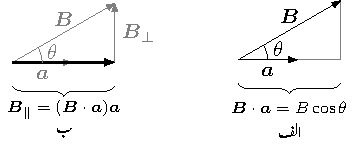
\includegraphics{figVectorComponentAlongUnitVector}
\caption{کسی بھی سمت میں سمتیہ کے جزو کا حصول۔}
\label{شکل_سمتیہ_کسی_سمت_میں_جزو}
\end{figure}
شکل \حوالہ{شکل_سمتیہ_کسی_سمت_میں_جزو}-الف میں سمتیہ \عددیء{\kvec{B}} اور اکائی سمتیہ \عددیء{\kvec{a}}  دکھائے گئے ہیں۔ان کا غیر سمتی ضرب
\begin{align*}
\kvec{B} \cdot \kvec{a} = \abs{\kvec{B}} \abs{\kvec{a}} \cos \theta=B \cos \theta
\end{align*}
کے برابر ہے۔شکل سے واضح ہے کہ یہی \عددیء{\kvec{a}} کی سمت میں \عددیء{\kvec{B}} کے جزو کا طول \عددیء{B_{\parallel}}\حاشیہد{\عددیء{B_{\parallel}} لکھتے ہوئے زیرنوشت میں دو متوازی لکیریں  یہ بتلاتی ہیں کہ \عددیء{\kvec{B}} کا یہ وہ حصہ ہے جو \عددیء{\kvec{a}} کے متوازی ہے۔اسی طرح عمودی مقدار کو عموماً \عددیء{\perp} کی علامت سے ظاہر کیا جاتا ہے۔} ہے۔یوں کسی بھی سمت میں \عددیء{\kvec{B}} کے جزو کا طول حاصل کرنے کی خاطر \عددیء{\kvec{B}} اور اس سمت کی اکائی سمتیہ کا غیر سمتی ضرب حاصل کریں۔یوں حاصل طول کا اکائی سمتیہ کے ساتھ ضرب یعنی \عددیء{(\kvec{B} \cdot \kvec{a}) \kvec{a}} سے اکائی سمتیہ کی سمت میں \عددیء{\kvec{B}} کا سمتی جزو  حاصل ہوتا ہے۔ شکل \حوالہ{شکل_سمتیہ_کسی_سمت_میں_جزو}-ب میں \عددیء{\kvec{a}} کی سمت میں \عددیء{\kvec{B}} کا سمتی جزو \عددیء{\kvec{B}_\parallel} دکھایا گیا ہے۔شکل سے واضح ہے کہ \عددیء{\kvec{B}} سے \عددیء{B_{\parallel} \kvec{a}} منفی کرنے سے  \عددیء{B_\perp} حاصل ہوتا ہے جو \عددیء{\kvec{B}} کا وہ جزو ہے جو \عددیء{\kvec{a}} کے عمودی ہے۔

غیر سمتی ضرب کا حاصل جواب دو صورتوں میں صفر کے برابر ہوتا ہے۔پہلی صورت وہ ہے جب دونوں سمتیوں میں سے کم از کم ایک سمتیہ کا طول صفر کے برابر ہو۔دوسری صورت وہ ہے جب دونوں سمتیات آپس میں عمودی ہوں۔عمودی ہونے کی صورت میں ان کے مابین نوے درجے کا زاویہ ہو گا اور \عددیء{\cos 90=0} کے برابر ہوتا ہے۔یوں دو سمتیوں کے نقطہ ضرب صفر کے برابر ہونے  سے اخذ کیا جاتا ہے کہ یہ آپس میں عمودی ہیں۔ 
%=================

\ابتدا{مثال}
شکل \حوالہ{شکل_سمتیہ_مثال_عمودی_سمتیات_کا_نقطہ_ضرب_صفر} میں تین نقطے \عددیء{M(1,5,6)}، \عددیء{N(4,3,1)} اور \عددیء{P(1,1,4)} دئے گئے ہیں۔\عددیء{M}  اور \عددیء{N} سے گزرتی سیدھی لکیر سے \عددیء{P} کا عمودی فاصلہ حاصل کریں۔ 
\begin{figure}
\centering
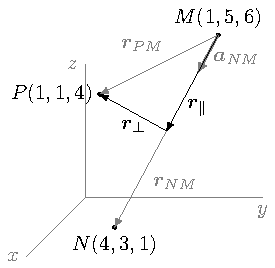
\includegraphics{figVectorExampleOrthognalVectorsHaveZeroDotProdcut}
\caption{متوازی اور عمودی اجزاء۔}
\label{شکل_سمتیہ_مثال_عمودی_سمتیات_کا_نقطہ_ضرب_صفر}
\end{figure}

حل:\عددیء{M} سے \عددیء{N} تک سمتیہ \عددیء{\kvec{r}_{NM}=3\ax-2\ay-5\az} ہے جس کا طول \عددیء{\abs{\kvec{r}_{NM}}=\sqrt{38}} ہے۔یوں اس سمت میں اکائی سمتیہ \عددیء{\kvec{a}_{NM}=\tfrac{3\ax-2\ay-5\az}{\sqrt{38}}} ہو گا۔ اسی طرح \عددیء{M} سے \عددیء{P} تک سمتیہ \عددیء{\kvec{r}_{PM}=-4\ay-2\az} ہے۔\عددیء{\kvec{a}_{NM}} کی سمت میں \عددیء{\kvec{r}_{PM}} کا طول
\begin{align*}
r_{\parallel}=\kvec{r}_{PM} \cdot \kvec{a}_{NM}&=(-4\ay-2\az) \cdot \left(\frac{3\ax-2\ay-5\az}{\sqrt{38}}\right) \\
&=\frac{0+8+10}{\sqrt{38}}=\frac{18}{\sqrt{38}}
\end{align*}
ہے یوں \عددیء{\kvec{a}_{NM}} سمت میں \عددیء{\kvec{r}_{PM}} کا سمتی جزو
\begin{align*}
\kvec{r}_{\parallel}=r_{\parallel} \kvec{a}_{NM}=\frac{18}{\sqrt{38}}\left(\frac{3\ax-2\ay-5\az}{\sqrt{38}}\right)=\frac{18}{38} (3\ax-2\ay-5\az)
\end{align*}
ہے۔\عددیء{\kvec{r}_{PM}} سے \عددیء{\kvec{r}_{\parallel}} منفی کرنے سے لکیر سے \عددیء{P} تک عمودی سمتیہ \عددیء{\kvec{r}_\perp} حاصل ہوتا ہے
\begin{align*}
\kvec{r}_{\perp}=\kvec{r}_{PM}-\kvec{r}_{\parallel}&=(-4\ay-2\az)-\frac{18}{38} (3\ax-2\ay-5\az)\\
&=\frac{-27\ax-58\ay+7\az}{19}
\end{align*}
جس کا طول \عددیء{\tfrac{\sqrt{27^2+58^2+7^2}}{19}=3.3873} ہے۔یوں \عددیء{P} کا لکیر سے عمودی فاصلہ \عددیء{3.3873} ہے۔

\عددیء{\kvec{r}_{\parallel}} اور \عددیء{\kvec{r}_\perp} آپس میں عمودی ہیں لہٰذا ان  کا نقطہ ضرب
\begin{align*}
\kvec{r}_\parallel \cdot \kvec{r}_\perp&=\frac{18}{38} (3\ax-2\ay-5\az) \cdot \left(\frac{-27\ax-58\ay+7\az}{19}\right)\\
&=\frac{18}{722}(-81+116-35)\\
&=0
\end{align*}
صفر کے برابر ہے۔
\انتہا{مثال}
%===================

شکل \حوالہ{شکل_سمتیہ_مثال_عمودی_سمتیات_کا_نقطہ_ضرب_صفر} میں اگر \عددیء{M} پر \عددیء{\kvec{r}_{NM}} کی دُم رکھی جائے تب  \عددیء{\kvec{r}_{NM}} کی نوک \عددیء{N} کا مقام تعین کرتا ہے۔عموماً کسی بھی نقطے کا مقام محدد کے مرکز \عددیء{(0,0,0)} کی نسبت سے طے کیا جاتا ہے۔ایسا سمتیہ جس کی دُم مرکز پر رکھتے ہوئے اس کی نوک نقطے کا مقام طے کرے  \اصطلاح{ہٹاو سمتیہ} سمتیہ\فرہنگ{ہٹاو سمتیہ}\فرہنگ{سمتیہ!ہٹاو}\حاشیہب{displacement vector}\فرہنگ{displacement vector} کہلاتا ہے۔اگر ہٹاو سمتیہ کو مرکز سے ہٹایا جائے تب ظاہر ہے اس کی نوک اصل مقام طے کرنے سے قاصر ہو گی۔
%=======================================
\ابتدا{مثال}
شکل \حوالہ{شکل_سمتیہ_مثال_عمودی_سمتیات_کا_نقطہ_ضرب_صفر} میں \عددیء{M} سے شروع ہوتے اور  \عددیء{N} جانب بڑھتی سیدھی لکیر پر کسی بھی نقطے کا مقام تعین کرنے والا ہٹاو سمتیہ حاصل کریں۔

حل:مرکز \عددیء{(0,0,0)} سے  نقطہ \عددیء{M} تک کا سمتیہ \عددیء{\kvec{r}_M=1\ax+5\ay+6\az} ہے جبکہ \عددیء{M} سے \عددیء{N} جانب اکائی سمتیہ \عددیء{\kvec{a}_{NM}} گزشتہ مثال میں حاصل کیا گیا۔اکائی سمتیہ \عددیء{\kvec{a}_{NM}} کی سمت میں  \عددیء{M} سے \عددیء{s} فاصلے پر نقطہ \عددیء{Q} تک کا سمتیہ \عددیء{s\kvec{a}_{NM}} ہے۔یوں مرکز سے  \عددیء{Q} تک سمتیہ \عددیء{\kvec{r}_Q=\kvec{r}_M+s\kvec{a}_{NM}} ہو گا۔
\begin{align*}
\kvec{r}_Q=(1\ax+5\ay+6\az) +s \left(\frac{3\ax-2\ay-5\az}{\sqrt{38}}\right)
\end{align*}   
اس مساوات میں \عددیء{s} متغیرہ ہے جسے تبدیل کرتے ہوئے سیدھی لکیر پر کسی بھی نقطہ \عددیء{Q} تک پہنچا جا سکتا ہے۔
\انتہا{مثال}
%==========================
\ابتدا{مثال}
\عددیء{z=z_0} پر \عددیء{1\az} کے عمودی سیدھی سطح کی مساوات حاصل کریں جہاں \عددیء{z_0} مستقل ہے۔ 

حل:نقطہ \عددیء{N_1(0,0,z_0)} سے کسی بھی نقطہ \عددیء{N_2(x,y,z)} تک کا سمتیہ \عددیء{\kvec{r}_{21}=x\ax+y\ay+(z-z_0)\az} ہے۔سطح پر کسی بھی سمتیہ اور سطح کے عمودی سمتیہ آپس میں نوے درجے زاویہ پر پائے جاتے ہیں لہٰذا ان کا غیر سمتی ضرب صفر کے برابر ہو گا۔یوں اگر \عددیء{N_2} اسی عمودی سطح پر پایا جائے تب
\begin{align*}
1\az \cdot [x\ax+y\ay+(z-z_0)\az]=z-z_0=0
\end{align*}
ہو گا جس سے اس سطح کی مساوات \عددیء{z=z_0} حاصل ہوتی ہے۔

اس قیمت کو \عددیء{\kvec{r}_{21}} میں پُر کرتے ہوئے \عددیء{\kvec{r}_{21}=x\ax+y\ay} حاصل ہوتا ہے جہاں \عددیء{x} اور \عددیء{y} آزاد متغیرات ہیں۔چونکہ مرکز سے \عددیء{N_1} کا ہٹاو سمتیہ \عددیء{\kvec{r}_{10}=z_0\az} ہے لہٰذا \عددیء{z=z_0} سطح پر کسی بھی نقطہ \عددیء{N_2} کا ہٹاو سمتیہ یعنی سطح کی سمتی مساوات  \عددیء{\kvec{r}_{20}=x\ax+y\ay+z_0\az} ہو گی۔
\انتہا{مثال}
%==========
\ابتدا{مشق}
مرکز سے \عددیء{(2,1,3)} تک کی سمتیہ ایک سیدھی سطح کی عمودی سمتیہ ہے۔اس سطح کی  مساوات حاصل کریں۔

جواب:\عددیء{2x+y+3z=14}
\انتہا{مشق}
%============
\حصہ{سمتی ضرب یا صلیبی ضرب}

دو سمتیات \عددیء{\kvec{A}} اور \عددیء{\kvec{B}} کے \اصطلاح{سمتی ضرب}\فرہنگ{سمتی ضرب}\فرہنگ{صلیبی ضرب}\حاشیہب{vector product}\فرہنگ{vector product} کا حاصل جواب سمتیہ ہوتا ہے جس کا طول \عددیء{\kvec{A}} کی مقدار ضربِ  \عددیء{\kvec{B}} کی مقدار ضربِ سمتیوں کے مابین چھوٹے زاویے کے سائن کے برابر ہے۔حاصل سمتیہ \عددیء{\kvec{A}} اور \عددیء{\kvec{B}} سمتیات کی عمودی سمت  میں ہوتا ہے جسے اکائی عمودی سمتیہ \عددیء{\kvec{a}_N} سے ظاہر کیا جائیگا۔
\begin{align}\label{مساوات_سمتیہ_سمتی_ضرب}
\kvec{A} \times \kvec{B}=\abs{\kvec{A}} \abs{\kvec{B}} \sin \theta_{AB} \kvec{a}_N
\end{align}
جس سیدھی سطح پر \عددیء{\kvec{A}} اور \عددیء{\kvec{B}} دونوں پائے جائیں، \عددیء{\kvec{a}_N} اس سطح کے دو عمودی سمتیات میں سے ایک ہے۔\عددیء{\kvec{a}_N} کو \اصطلاح{دائیں ہاتھ کے قانون}\فرہنگ{دائیں ہاتھ!قانون}\حاشیہب{right hand rule}\فرہنگ{right hand rule} سے یوں حاصل کیا جا سکتا ہے۔

\ابتدا{قانون}\شناخت{قانون_سمتیہ_دائیں_ہاتھ_قانون}
دائیں ہاتھ کی ہتھیلی  سیدھی اور انگوٹھے کو بقایا چار انگلیوں کے عمود میں رکھتے ہوئے پہلی انگلی کو \عددیء{\kvec{A}} اور  دوسری انگلی کو \عددیء{\kvec{B}} کی سمت میں رکھیں۔اس صورت میں انگوٹھا \عددیء{\kvec{a}_N} کی سمت میں ہو گا۔  
\انتہا{قانون}

اگر دونوں سمتیات کی دُم ایک ہی جگہ پر نہ ہو تب ان کے مابین زاویہ دریافت کرنے کی  خاطر سمتیوں کی سمت تبدیل کئے بغیر انہیں ایک نقطے پر منتقل کیا جا سکتا ہے۔سمتی ضرب کو سمتیوں کے درمیان صلیبی نشان \عددیء{\times} سے ظاہر کیا جاتا ہے۔اسی وجہ سے اسے \اصطلاح{صلیبی ضرب}\حاشیہب{cross product}\فرہنگ{cross product} بھی کہا جاتا ہے اور \عددیء{\kvec{A} \times \kvec{B}} کو "\عددیء{\kvec{A}} صلیب \عددیء{\kvec{B}}" پڑھا جاتا ہے۔سمتی ضرب میں سمتیوں کی ترتیب نہایت اہم ہے اور انہیں الٹانے سے حاصل جواب کی سمت الٹی ہو جاتی ہے۔
\begin{align}\label{مساوات_سمتیہ_صلیبی_ضرب_ترتیب_الٹاتے_منفی_سمت}
\kvec{A} \times \kvec{B}=- \kvec{B} \times \kvec{A}
\end{align}

اکائی سمتیات \عددیء{\ax} اور \عددیء{\ay} کے مابین نوے درجے کا زاویہ ہے  اور \عددیء{\sin 90\degree=1} کے برابر ہے جبکہ دائیں ہاتھ کے قانون سے ان کے صلیبی ضرب کی سمت \عددیء{\az} حاصل ہوتی ہے۔یوں \عددیء{\ax \times \ay=\az} کے برابر ہے۔اسی طرح \عددیء{\ay \times \az=\ax} اور \عددیء{\az \times \ax=\ay} کے برابر حاصل ہوتے ہیں۔مساوات \حوالہ{مساوات_سمتیہ_صلیبی_ضرب_ترتیب_الٹاتے_منفی_سمت} کے تحت یوں \عددیء{\ay \times \ax=-\az}، \عددیء{\az \times \ay=-\ax} اور \عددیء{\ax \times \az=-\ay} لکھے جا سکتے ہیں۔دو متوازی سمتیوں کے درمیان صفر درجے کا زاویہ ہوتا ہے اور \عددیء{\sin 0 =0} کے برابر ہے لہٰذا \عددیء{\ax \times \ax=0} کے برابر ہے۔اسی طرح \عددیء{\ay \times \ay=0} اور \عددیء{\az \times \az=0} کے برابر ہیں۔ان تمام جوابات کو ایک جگہ لکھتے ہیں۔
\begin{gather}
\begin{aligned}\label{مساوات_سمتیہ_کارتیسی_اکائی_سمتیات_صلیبی_ضرب}
\ax \times \ay &=\az & \ay \times \az&=\ax & \az \times \ax&=\ay\\
\ax \times \ax&=0 & \ay \times \ay&=0 & \az \times \az&=0
\end{aligned}
\end{gather}
%=================

یہی جوابات شکل \حوالہ{شکل_سمتیہ_صلیبی_ضرب_مثبت_دائرہ} کی مدد سے حاصل کئے جا سکتے ہیں۔اس شکل میں گھڑی کی الٹ سمت مثبت سمت ہے۔یوں اگر \عددیء{\ax \times \ay} حاصل کرنا ہو تو شکل میں \عددیء{\ax} سے شروع ہو کر \عددیء{\ay} کی جانب کم راستے پر چلتے ہوئے  \عددیء{\az} حاصل ہوتا ہے۔ساتھ ہی ساتھ چونکہ \عددیء{\ax} سے \عددیء{\ay} جانے کی خاطر  مثبت راستہ اختیار کیا گیا لہٰذا جواب مثبت یعنی \عددیء{+\az} ہو گا۔اس کے برعکس \عددیء{\az \times \ay} حاصل کرنے کی خاطر \عددیء{\az} سے \عددیء{\ay} جانب کم راستے پر چلتے ہوئے \عددیء{\ax} حاصل ہوتا ہے البتہ یہ راستہ گھڑی کے الٹ سمت یعنی منفی سمت میں ہے لہٰذا جواب \عددیء{-\ax} ہو گا۔ 
\begin{figure}
\centering
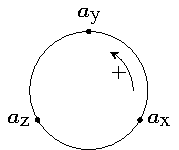
\includegraphics{figVectorCartesianRightHandCircle}
\caption{صلیبی ضرب کا حصول۔}
\label{شکل_سمتیہ_صلیبی_ضرب_مثبت_دائرہ}
\end{figure}

مساوات \حوالہ{مساوات_سمتیہ_کارتیسی_اکائی_سمتیات_صلیبی_ضرب} کی  مدد سے \عددیء{\kvec{A}=A_x\ax+A_y\ay+A_z\az} اور \عددیء{\kvec{B}=B_x\ax+B_y\ay+B_z\az} کی صلیبی ضرب
\begin{align*}
\kvec{A} \times \kvec{B}&=(A_x\ax+A_y\ay+A_z\az) \times (B_x\ax+B_y\ay+B_z\az)\\
&=A_x B_x \ax \times \ax+A_x B_y \ax \times \ay+A_x B_z \ax \times \az\\
& \quad \quad +A_y B_x \ay \times \ax+A_y B_y \ay \times \ay+A_y B_z \ay \times \az \\
&\quad \quad +A_z B_x \az \times \ax+A_z B_y \az \times \ay+A_z B_z \az \times \az
\end{align*}
کو
\begin{align}
\kvec{A} \times \kvec{B}=(A_y B_z-A_z B_y)\ax+(A_z B_x-A_x B_z)\ay+(A_x B_y-A_y B_x)\az
\end{align}
لکھا جا سکتا ہے۔اس جواب کو قالب کے حتمی قیمت کی شکل میں یوں لکھا جا سکتا ہے۔
\begin{align}\label{مساوات_سمتیات_سمتی_ضرب_قالب_شکل}
\kvec{A} \times \kvec{B}=\begin{vmatrix}
\ax & \ay & \az\\
A_x & A_y & A_z\\
B_x & B_y & B_z
\end{vmatrix}
\end{align}
مندرجہ بالا قالب کو کتاب کے آخر میں صفحہ \حوالہصفحہ{ضمیمہ_خطی_الجبرا} پر ضمیمے میں آپ کے آسانی کے لئے دوبارہ پیش کیا گیا ہے۔اس ضمیمے کو ایک مرتبہ دیکھ لیں۔
یوں اگر \عددیء{\kvec{A}=2\ax-3\ay+1\az} اور \عددیء{\kvec{B}=6\ax+5\ay-4\az} ہوں تب
\begin{align*}
\kvec{A} \times \kvec{B}&=\begin{vmatrix*}[r]
\ax & \ay & \az\\
2 & -3 & 1\\
6 & 5 & -4
\end{vmatrix*}\\
&=[(-3)(-4)-(1)(5)]\ax-[(2)(-4)-(1)(6)]\ay+[(2)(5)-(-3)(6)]\az\\
&=7\ax+14\ay+28\az
\end{align*}
ہو گا۔
%===========
\ابتدا{مثال}
\عددیء{N_1(2,3,1)}، \عددیء{N_2(1,6,5)} اور \عددیء{N_3(-2,-3,2)} سیدھی سطح پر پائے جاتے ہیں۔اس سطح کی مساوات حاصل کریں۔

حل:
\begin{align*}
\kvec{r}_{21}&=(1-2)\ax+(6-3)\ay+(5-1)\az=-1\ax+3\ay+4\az\\
\kvec{r}_{31}&=(-2-2)\ax+(-3-3)\ay+(2-1)\az=-4\ax-6\ay+1\az
\end{align*}
کے سمتی ضرب سے ان کا عمودی سمتیہ حاصل ہو گا۔
\begin{align*}
\kvec{r}_N&=(-1\ax+3\ay+4\az) \times (-4\ax-6\ay+1\az)\\
&=6\az+1\ay+12\az+3\ax-16\ay+24\ax\\
&=27\ax-15\ay+18\az
\end{align*}
سطح پر دئے گئے تین نقطوں سے سطح پر کسی بھی نقطہ \عددیء{N_4(x,y,z)} تک کا سمتیہ اس عمودی سمتیہ کے نوے درجے زاویہ پر ہو گا اور یوں ان کا غیر سمتی ضرب صفر کے برابر ہو گا۔\عددیء{N_1} سے \عددیء{N_4} تک سمتیہ \عددیء{\kvec{r}_{41}=(x-2)\ax+(y-3)\ay+(z-1)\az} کے استعمال سے
\begin{align*}
\kvec{r}_{41} \cdot \kvec{r}_{N}=[(x-2)\ax+(y-3)\ay+(z-1)\az] \cdot (27\ax-15\ay+18\az)=0
\end{align*}
لکھ کر
\begin{align*}
27(x-2)-15(y-3)+18(z-1)=0
\end{align*}
سے
\begin{align*}
27x-15y+18z=27
\end{align*}
سیدھی سطح کی مساوات حاصل ہوتی ہے۔ایسی مساوات میں \عددیء{x}، \عددیء{y} اور \عددیء{z} کے عددی سر  عمودی سمتیہ میں \عددیء{\ax}، \عددیء{\ay} اور \عددیء{\az} کے عددی سر ہوتے ہیں۔موجودہ مساوات میں عددی سر \عددیء{27}، \عددیء{-15} اور \عددیء{18} ہیں۔

سطح کی مساوات سے \عددیء{z=\tfrac{9-9x+5y}{6}} لکھا جا سکتا ہے۔سطح پر \عددیء{N_4} کی تعین کنندہ مساوات \عددیء{\kvec{r}=x\ax+y\ay+z\az} میں \عددیء{z} کی قیمت پُر کرتے ہوئے  سطح کی سمتی مساوات 
\begin{align*}
\kvec{r}=x\ax+y\ay+\left(\frac{9-9x+5y}{6}\right)\az
\end{align*}
لکھی جا سکتی ہے جہاں \عددیء{x} اور \عددیء{y} آزاد متغیرات ہیں جبکہ \عددیء{z} کو بطور تابع متغیرہ لکھا گیا ہے۔
\انتہا{مثال}
%=========

\ابتدا{مشق}
\عددیء{\kvec{A}=1\ax+3\ay-2\az} اور \عددیء{\kvec{B}=5\ax-2\ay-3\az} کی صورت میں \عددیء{\kvec{A} \times \kvec{B}}، \عددیء{\kvec{B}\times \kvec{A}}، \عددیء{\kvec{A} \times \kvec{A}}، \عددیء{\kvec{a}_B \times \kvec{A}} اور \عددیء{\az \times (\ay \times \kvec{B})} حاصل کریں۔ 
\انتہا{مشق}
%========================

خلاء میں کسی بھی نقطے کا مقام کارتیسی محدد کے علاوہ دیگر طرز کے محدد سے بھی تعین کیا جا سکتا ہے۔ماہرین طبیعیات  تقریباً ایک درجن اقسام کے محددی نظام استعمال کرتے ہیں۔ہم اس کتاب میں کارتیسی نظام کے علاوہ دو مزید اقسام کے محددی نظام استعمال کریں گے۔آئیں انہیں پر غور کریں۔ 

\حصہ{گول نلکی محدد}
کارتیسی نظام میں کسی بھی نقطے کا مقام مرکز سے \عددیء{x}، \عددیء{y} اور \عددیء{z} سمتوں میں فاصلوں سے طے کیا جاتا ہے۔آئیں اب ایسا نظام دیکھیں جس میں ایک عدد زاویہ اور دو عدد فاصلے استعمال کرتے ہوئے کسی بھی نقطے کا مقام طے ہو۔
 \begin{figure}
\centering
\begin{subfigure}{0.5\textwidth}
\centering
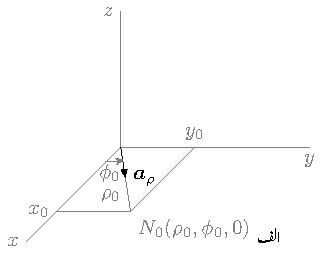
\includegraphics{figVector2and3Dcylindrical}
\end{subfigure}%
%
\begin{subfigure}{0.5\textwidth}
\centering
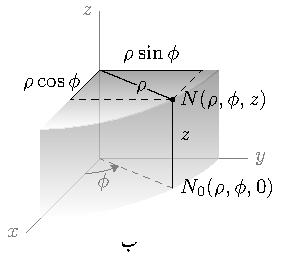
\includegraphics{figVectorCylindricalToCartesian}
\end{subfigure}%
\caption{نلکی محدد}
\label{شکل_سمتیہ_نلکی_محدد}
\end{figure}

شکل \حوالہ{شکل_سمتیہ_نلکی_محدد}-الف میں \عددیء{z=0} سطح پر نقطہ \عددیء{N_0} دکھایا گیا ہے جسے کارتیسی محدد میں \عددیء{N_0(x_0,y_0,0)} لکھا جائے گا۔اگر مرکز سے \عددیء{N_0} تک سیدھی لکیر کی لمبائی \عددیء{\rho_0} اور \عددیء{x} محدد سے اس لکیر کا زاویہ \عددیء{\phi_0} ہو تب اسی نقطے
 کو \اصطلاح{گول نلکی محدد}\فرہنگ{نلکی!محدد}\حاشیہب{cylindrical coordinate system}\فرہنگ{cylindrical!coordinates} کے نظام میں \عددیء{N_0(\rho_0,\phi_0,0)} لکھا جاتا ہے۔اس کتاب میں گول نلکی محدد کا نام چھوٹا کر کے اسے \اصطلاح{نلکی محدد} پکارا جائے گا۔ اگر \عددیء{z=0} سطح پر مرکز سے نقطے کی جانب اکائی سمتیہ \عددیء{\arho} ہو تب مرکز سے نقطے تک سمتیہ کو
\begin{align}
\kvec{\rho}=\rho_0 \arho \quad \quad (\phi=\phi_0, \quad   z=0 )
\end{align}
   لکھا جا سکتا ہے۔نلکی  اور کارتیسی نظام میں  \عددیء{z} محدد یکساں ہیں۔

شکل \حوالہ{شکل_سمتیہ_نلکی_محدد} سے کارتیسی اور نلکی محدد کے تعلق اخذ کئے جا سکتے ہیں۔یوں نلکی محدد کے متغیرات \عددیء{(\rho,\phi,z)} سے کارتیسی متغیرات \عددیء{(x,y,z)} یوں حاصل ہوتے ہیں۔
\begin{gather}
\begin{aligned}
x&=\rho \cos \phi\\
y&=\rho \sin \phi\\
z&=z
\end{aligned}
\end{gather}
اسی طرح \عددیء{(x,y,z)} سے  \عددیء{(\rho,\phi,z)} یوں حاصل کئے جاتے ہیں۔
\begin{gather}
\begin{aligned}
\rho&=\sqrt{x^2+y^2} \quad \quad (\rho \ge 0)\\
\phi&=\tan^{-1} \frac{y}{x}\\
z&=z
\end{aligned}
\end{gather}
%
درج بالا دونوں تعلقات کو کتاب کے آخر میں صفحہ \حوالہصفحہ{ضمیمہ_محددی_تعلق} پر ضمیمے میں دوبارہ پیش کیا گیا ہے۔
\begin{figure}
\centering
\begin{subfigure}{0.5\textwidth}
\centering
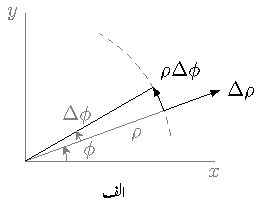
\includegraphics{figVectorCylindricalRadiusAngle}
\end{subfigure}%
%
\begin{subfigure}{0.5\textwidth}
\centering
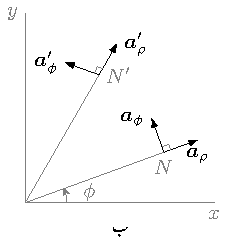
\includegraphics{figVectorCylindricalUnitVectors}
\end{subfigure}%
\caption{نلکی محدد میں متغیرات کے تبدیلی سے فاصلے کا حصول اور اکائی سمتیات۔}
\label{شکل_سمتیہ_نلکی_تبدیلی_متغیرات}
\end{figure}
مندرجہ بالا مساوات میں رداس کی صرف مثبت قیمت لی گئی۔ہم  رداس کی قیمت مثبت ہی لیتے ہیں۔

شکل \حوالہ{شکل_سمتیہ_نلکی_تبدیلی_متغیرات}-الف میں \عددیء{\phi} زاویہ پر \عددیء{\rho} رداس کا ہلکی سیاہی میں دکھایا سمتیہ نقطہ \عددیء{N} ہے۔
اس شکل میں \عددیء{\phi} اور \عددیء{z} تبدیل کئے بغیر \عددیء{\rho} کو \عددیء{\Delta \rho} بڑھتا دکھایا گیا ہے۔اس صورت میں سمتیہ کی نوک \عددیء{\Delta \rho} فاصلہ طے کرتی ہے۔نقطہ \عددیء{N} سے \عددیء{\Delta \rho} کی سمت میں اکائی سمتیہ جسے \عددیء{\arho} لکھا جاتا ہے، نلکی محدد کی  بنیادی اکائی سمتیہ ہے۔اس سمتیہ کو شکل \حوالہ{شکل_سمتیہ_نلکی_تبدیلی_متغیرات}-ب میں دکھایا گیا ہے۔

شکل \حوالہ{شکل_سمتیہ_نلکی_تبدیلی_متغیرات}-الف میں   \عددیء{\rho} اور \عددیء{z} تبدیل کئے بغیر \عددیء{\phi} کو \عددیء{\Delta \phi} بڑھا کر اسی سمتیہ کو گاڑھی سیاہی میں دوبارہ دکھایا گیا ہے۔آپ دیکھ سکتے ہیں کہ  سمتیہ کی نوک نے \عددیء{\rho} رداس کے گول دائرے پر حرکت کرتے ہوئے  \عددیء{\rho \Delta \phi} فاصلہ طے کیا۔یوں اگر زاویہ کو \عددیء{0} تا \عددیء{2\pi} ریڈیئن تبدیل کیا جائے  تو سمتیہ کی نوک گول دائرے پر ایک مکمل چکر کاٹے گی۔جیسے جیسے \عددیء{\Delta \phi} کو کم سے کم کیا جائے ویسے ویسے  \عددیء{\rho \Delta \phi}  گول دائرے کے مماس کی صورت اختیار کرے گی حتٰی کہ \عددیء{\dif \phi} کی صورت میں \عددیء{\rho \dif \phi} گول دائرے کا مماس ہو گا۔نقطہ \عددیء{N} پر بڑھتے \عددیء{\phi} جانب مماس کی سمت میں اکائی سمتیہ کو \عددیء{\aphi} لکھا جاتا ہے۔ اس سمتیہ کو شکل \حوالہ{شکل_سمتیہ_نلکی_تبدیلی_متغیرات}-ب میں دکھایا گیا ہے۔

اسی طرح اگر نقطہ \عددیء{N} پر صرف \عددیء{z} کو \عددیء{\Delta z} تبدیل کیا جائے تب سمتیہ کی نوک \عددیء{\Delta z} فاصلہ طے کرے گی۔ \عددیء{\Delta z} کی سمت میں اکائی سمتیہ جسے \عددیء{\az} لکھا جاتا ہے، نلکی محدد کی تیسری اور آخری بنیادی اکائی سمتیہ ہے۔نلکی محدد کے تین اکائی سمتیات \عددیء{\arho}، \عددیء{\aphi} اور \عددیء{\az} مل کر دائیں ہاتھ کا عمودی  نظام دیتے ہیں۔نقطہ \عددیء{(\rho_1,\phi_1,z_1)} پر نلکی محدد کے اکائی سمتیات کو شکل \حوالہ{شکل_سمتیہ_نلکی_اکائی_سمتیات_عمومی} میں دکھایا گیا ہے۔\عددیء{\arho} گول سطح \عددیء{\rho=\rho_1} کے عمودی ہے۔یہ \عددیء{\phi=\phi_1} اور \عددیء{z=z_1} سطحوں پر پایا جاتا ہے۔اسی طرح \عددیء{\aphi} سیدھی سطح  \عددیء{\phi=\phi_1} کے عمودی ہے۔ یہ \عددیء{z=z_1} سطح پر پایا جاتا ہے اور \عددیء{\rho=\rho_1} نلکی سطح کا مماس ہے۔\عددیء{\az} اکائی سمتیہ \عددیء{z=z_1} سطح کے عمودی ہے۔یہ \عددیء{\rho=\rho_1} اور \عددیء{\phi=\phi_1} سطحوں پر پایا جاتا ہے۔ 
\begin{figure}
\centering
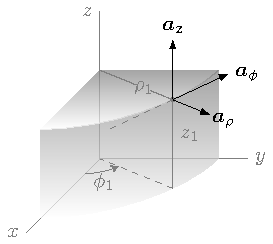
\includegraphics{figVectorCylindricalUnitVectorDirectionsInThreeD}
\caption{نلکی محدد کے اکائی سمتیات۔}
\label{شکل_سمتیہ_نلکی_اکائی_سمتیات_عمومی}
\end{figure}

دائیں ہاتھ کے عمودی نظام میں سمتی ضرب کا حاصل جواب صفحہ \حوالہصفحہ{قانون_سمتیہ_دائیں_ہاتھ_قانون} پر دئے گئے دائیں ہاتھ کے قانون کی مدد سے حاصل کیا جاتا ہے ۔ یوں
\begin{align}\label{مساوات_سمتیات_نلکی_اکائی_سمتیات_کا_سمتی_ضرب}
\arho \times \aphi=\az, \quad \aphi \times \az=\arho, \quad \az \times \arho=\aphi
\end{align}
لکھا جا سکتا ہے۔یہی جوابات شکل \حوالہ{شکل_سمتیہ_نلکی_صلیبی_ضرب_مثبت_دائرہ} سے بھی اخذ کئے جا سکتے ہیں۔
\begin{figure}
\centering
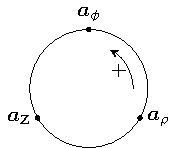
\includegraphics{figVectorCylindricalRightHandCircle}
\caption{صلیبی ضرب کی حاصل اکائی سمتیہ۔}
\label{شکل_سمتیہ_نلکی_صلیبی_ضرب_مثبت_دائرہ}
\end{figure}

کسی سمتیہ کا خود سمتی ضرب صفر کے برابر ہوتا ہے لہٰذا
\begin{align}\label{مساوات_سمتیات_نلکی_اکائی_سمتیات_کا_سمتی_ضرب_ب}
\arho \times \arho=0, \quad \aphi \times \aphi =0, \quad \az \times \az=0
\end{align}
لکھا جا سکتا ہے جبکہ کسی بھی اکائی سمتیہ کا خود غیر سمتی ضرب ایک کے برابر ہوتا ہے لہٰذا 
\begin{align}
\arho \cdot \arho=1, \quad \aphi \cdot \aphi =1, \quad \az \cdot \az =1
\end{align}
لکھا جا سکتا ہے۔اسی طرح کسی بھی دو عمودی سمتیات  کا غیر سمتی ضرب صفر کے برابر ہوتا ہے یعنی
\begin{align}
\arho \cdot \aphi=0, \quad \aphi \cdot \az =0, \quad \az \cdot \arho =0
\end{align}

غیر سمتی ضرب کو  \اصطلاح{کرونیکر ڈیلٹا} کی مدد سے یوں لکھا جا سکتا ہے۔
\begin{align}
\kvec{a}_i \cdot \kvec{a}_j=\delta_{ij}
\end{align}
جہاں
\begin{align}
\delta_{ij}=
\begin{cases}
0 \quad  \quad  i\ne j \; \textup{ اگر}\\
1 \quad \quad i=j \; \textup{ اگر}
\end{cases}
\end{align}
کے برابر ہے۔

آپ دیکھتے ہیں کہ کسی بھی نقطہ \عددیء{N(\rho,\phi,z)} پر  اکائی سمتیات حاصل کرنے کی خاطر محدد کے متغیرات \عددیء{\rho}، \عددیء{\phi} اور \عددیء{z} کو  باری باری انتہائی کم بڑھایا جاتا ہے۔جس سمت میں نقطہ حرکت کرے، اسی سمت میں اکائی سمتیہ ہو گی۔شکل \حوالہ{شکل_سمتیہ_نلکی_تبدیلی_متغیرات}-ب میں دو مختلف نقاط \عددیء{N} اور \عددیء{N'} پر نلکی محدد کے عمودی اکائی سمتیات دکھائے گئے ہیں۔آپ دیکھ سکتے ہیں کہ نلکی محدد کے عمودی اکائی سمتیات کی سمت کا دارومدار اس نقطے پر ہے جہاں انہیں حاصل کیا جائے۔آپ جانتے ہیں کہ کارتیسی نظام میں نقطے کا مقام تبدیل کرنے سے کارتیسی اکائی سمتیات تبدیل نہیں ہوتے۔یوں نلکی محدد کے اکائی سمتیات اٹل نہیں ہیں۔یہ ایک انتہائی اہم حقیقت ہے جو تکمل لیتے وقت پیچیدگیاں پیدا کرتا ہے۔تکمل لیتے وقت کارتیسی اکائی سمتیات اٹل ہونے کی بنا پر تکمل کے باہر لے جائے جا سکتے ہیں جبکہ نلکی محدد کے  \عددیء{\arho} اور \عددیء{\aphi} اکائی سمتیات کو تکمل کے باہر نہیں لے جایا جا سکتا۔یاد رہے کہ کسی بھی نقطہ \عددیء{N} پر حاصل کئے گئے \عددیء{\arho}، \عددیء{\aphi} اور \عددیء{\az} آپس میں عمودی ہوں گے جبکہ کسی اور نقطہ \عددیء{N'} پر حاصل کئے گئے \عددیء{\arho'}، \عددیء{\aphi'} اور \عددیء{\az} آپس میں عمودی ہوں گے۔

\جزوحصہ{نلکی اکائی سمتیات کا کارتیسی اکائی سمتیات کے ساتھ غیر سمتی ضرب}
شکل \حوالہ{شکل_سمتیہ_نلکی_کارتیسی_اکائی_غیر_سمتی_ضرب}-الف میں نقطہ \عددیء{N} پر اکائی سمتیات \عددیء{\arho}، \عددیء{\ax} اور \عددیء{\ay} دکھائے گئے ہیں۔\عددیء{\arho} اور  \عددیء{\ax} کے مابین زاویہ \عددیء{\phi} ہے جبکہ اکائی سمتیات کی لمبائی ایک ہوتی ہے لہٰذا
\begin{align}
\arho \cdot \ax=(1)(1)(\cos \phi)=\cos \phi
\end{align}
ہے۔\عددیء{\arho} اور  \عددیء{\ay} کے مابین زاویہ \عددیء{(90^\circ-\phi)} ہے  لہٰذا
\begin{align}
\arho \cdot \ay=(1)(1)[\cos (90^\circ-\phi)]=\sin \phi
\end{align}
کے برابر ہے۔اس مساوات میں
\begin{align*}
\cos(\alpha-\beta)=\cos \alpha \cos \beta+\sin \alpha \sin \beta
\end{align*}
کو استعمال کرتے ہوئے \عددیء{\cos(90^\circ-\phi)=\sin \phi} لکھا گیا ہے۔شکل \حوالہ{شکل_سمتیہ_نلکی_کارتیسی_اکائی_غیر_سمتی_ضرب}-ب میں نقطہ \عددیء{N} پر اکائی سمتیات \عددیء{\aphi}، \عددیء{\ax} اور \عددیء{\ay} دکھائے گئے ہیں۔\عددیء{\aphi} اور  \عددیء{\ax} کے مابین زاویہ \عددیء{(90^\circ+\phi)} ہے  لہٰذا
\begin{align}
\aphi \cdot \ax=(1)(1)[\cos (90^\circ+\phi)]=-\sin \phi
\end{align}
ہے۔\عددیء{\aphi} اور  \عددیء{\ay} کے مابین زاویہ \عددیء{\phi} ہے  لہٰذا
\begin{align}
\aphi \cdot \ay=(1)(1)(\cos \phi)=\cos \phi
\end{align}
کے برابر ہے۔\عددیء{\az} کا \عددیء{\ax} اور \عددیء{\ay} کے ساتھ غیر سمتی ضرب صفر کے برابر ہے۔اس کی وجہ ان کے مابین نوے درجے کا زاویہ ہے۔ان تمام غیر سمتی ضرب کو جدول \حوالہ{جدول_سمتیہ_نلکی_کارتیسی_اکائی_غیر-سمتی_ضرب} میں یکجا کیا گیا ہے۔
\begin{figure}
\centering
\begin{subfigure}{0.5\textwidth}
\centering
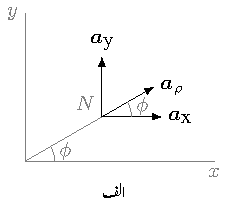
\includegraphics{figVectorCylindricalXandRhoDotProduct}
\end{subfigure}%
%
\begin{subfigure}{0.5\textwidth}
\centering
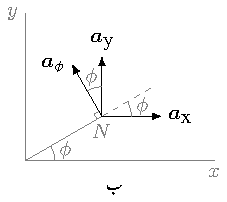
\includegraphics{figVectorCylindricalXandPhiDotProduct}
\end{subfigure}%
\caption{نلکی اکائی سمتیات کا کارتیسی اکائی سمتیات کے ساتھ غیر سمتی ضرب۔}
\label{شکل_سمتیہ_نلکی_کارتیسی_اکائی_غیر_سمتی_ضرب}
\end{figure}%
%
%
\begin{table}
\caption{نلکی اکائی سمتیات کا کارتیسی اکائی سمتیات کے ساتھ غیر سمتی ضرب۔}
\centering
\begin{tabular}{l | r r r}
 & $\ax$ & $\ay$ & $\az$ \\
\hline
$\arho$ & $\cos \phi$ & $\sin \phi $& $0$\\
$\aphi$ &$-\sin \phi$ &$ \cos \phi$ &$ 0$\\
$\az$ & $0$ &$ 0$ &$1$
\end{tabular}
\label{جدول_سمتیہ_نلکی_کارتیسی_اکائی_غیر-سمتی_ضرب}
\end{table}
%
\begin{figure}
\centering
\begin{subfigure}{0.5\textwidth}
\centering
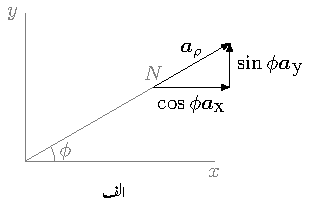
\includegraphics{figVectorCylindricalRhoToCartesianConversion}
\end{subfigure}%
%
\begin{subfigure}{0.5\textwidth}
\centering
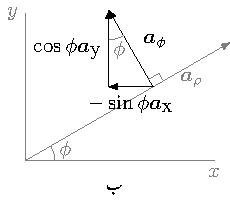
\includegraphics{figVectorCylindricalPhiToCartesianConversion}
\end{subfigure}%
\caption{\عددیء{\arho} اور \عددیء{\aphi} کا کارتیسی نظام میں تبادلہ۔}
\label{شکل_سمتیہ_کارتیسی_نظام_میں_نلکی_رداس_اکائی}
\end{figure}%

\جزوحصہ{نلکی اور کارتیسی اکائی سمتیات کا تعلق}
شکل \حوالہ{شکل_سمتیہ_کارتیسی_نظام_میں_نلکی_رداس_اکائی}-الف میں نقطہ \عددیء{N} پر اکائی سمتیہ \عددیء{\arho} دکھایا گیا ہے۔آپ دیکھ سکتے ہیں کہ کارتیسی محدد میں اسی اکائی سمتیہ کو دو عدد سمتیات کی مدد سے لکھا جا سکتا ہے۔\عددیء{\arho} کی لمبائی ایک کے برابر ہے۔یوں مسئلہ فیثاغورث کی مدد سے
\begin{gather}
\begin{aligned}\label{مساوات_سمتیہ_اکائی_رداس_کارتیسی_میں}
\arho&=\cos \phi \ax+\sin \phi \ay\\
&=\frac{x}{\sqrt{x^2+y^2}} \ax+\frac{y}{\sqrt{x^2+y^2}} \ay
\end{aligned}
\end{gather}
 لکھا جا سکتا ہے جہاں دوسرے قدم پر تمام نلکی محدد کے متغیرات کو کارتیسی متغیرات کی شکل میں لکھا گیا ہے۔شکل \حوالہ{شکل_سمتیہ_کارتیسی_نظام_میں_نلکی_رداس_اکائی}-ب میں نقطہ \عددیء{N} پر اکائی سمتیہ \عددیء{\aphi} دکھایا گیا ہے۔آپ دیکھ سکتے ہیں کہ کارتیسی محدد میں اسی اکائی سمتیہ کو دو عدد سمتیات کی مدد سے یوں  لکھا جا سکتا ہے
\begin{gather}
\begin{aligned}\label{مساوات_سمتیہ_اکائی_زاویہ_کارتیسی_میں}
\aphi&=-\sin \phi \ax+\cos \phi \ay\\
&=-\frac{y}{\sqrt{x^2+y^2}} \ax+\frac{x}{\sqrt{x^2+y^2}} \ay
\end{aligned}
\end{gather}
جہاں دوسرے قدم پر تمام نلکی محدد کے متغیرات کو کارتیسی متغیرات کی شکل میں لکھا گیا ہے۔
%
\begin{figure}
\centering
\begin{subfigure}{0.5\textwidth}
\centering
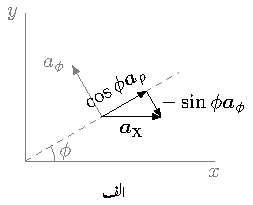
\includegraphics{figVectorCartesianXtoCylindricalConversion}
\end{subfigure}%
%
\begin{subfigure}{0.5\textwidth}
\centering
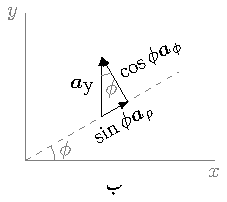
\includegraphics{figVectorCartesianYtoCylindricalConversion}
\end{subfigure}%
\caption{\عددیء{\ax} اور \عددیء{\ay} کا نلکی محدد میں تبادلہ۔}
\label{شکل_سمتیہ_نلکی_محدد_میں_کارتیسی_اکائی_سمتیات}
\end{figure}%

شکل \حوالہ{شکل_سمتیہ_نلکی_محدد_میں_کارتیسی_اکائی_سمتیات}-الف میں \عددیء{\ax} کا نلکی محدد میں تبادلہ دکھایا گیا ہے۔جس نقطے پر ایسا درکار ہو، اس نقطے پر \عددیء{\ax} کی دُم رکھیں۔مرکز سے نقطے تک نقطہ دار سیدھی لکیر کھینچتے ہوئے اسے مزید آگے بڑھائیں۔اس نقطے پر \عددیء{\arho} اسی لکیر کی سمت میں ہو گا جبکہ \عددیء{\aphi} لکیر کے ساتھ نوے درجے کا زاویہ بنائے گا۔شکل میں \عددیء{\aphi} دکھایا گیا ہے۔جیسا شکل میں دکھایا گیا ہے، \عددیء{\ax} کی نوک سے نقطہ دار لکیر پر عمود بنائیں۔صاف ظاہر ہے کہ \عددیء{\ax} کو دو عدد سمتیات کی مدد سے لکھا جا سکتا ہے۔ان میں سے ایک سمتیہ \عددیء{\arho} کی سمت میں اور دوسرا سمتیہ \عددیء{\aphi} کی الٹ جانب کو ہو گا۔یوں
\begin{align}\label{مساوات_سمتیہ_اکائی_ایکس_نلکی_میں}
\ax=\cos \phi \arho-\sin \phi \aphi
\end{align}
لکھا جا سکتا ہے۔شکل \حوالہ{شکل_سمتیہ_نلکی_محدد_میں_کارتیسی_اکائی_سمتیات}-ب میں \عددیء{\ay} کا نلکی محدد میں تبادلہ دکھایا گیا ہے۔یہاں نقطہ پر \عددیء{\ay} کی دُم رکھتے ہوئے اس کی نوک سے نقطہ دار لکیر پر عمود کھینچا گیا ہے۔یوں
\begin{align}\label{مساوات_سمتیہ_اکائی_وائے_نلکی_میں}
\ay=\sin \phi \arho+\cos \phi \aphi
\end{align}
لکھا جا سکتا ہے۔

آئیں مساوات \حوالہ{مساوات_سمتیہ_اکائی_رداس_کارتیسی_میں} تا مساوات \حوالہ{مساوات_سمتیہ_اکائی_وائے_نلکی_میں} کو جدول \حوالہ{جدول_سمتیہ_نلکی_کارتیسی_اکائی_غیر-سمتی_ضرب} کی مدد سے حاصل کریں۔کسی بھی سمتیہ \عددیء{\kvec{A}} کو کارتیسی یا نلکی محدد میں لکھا جا سکتا ہے۔یوں
\begin{gather}
\begin{aligned}\label{مساوات_سمتیہ_سمتیہ_نلکی_کارتیسی_اشکال}
\kvec{A}&=A_x \ax+A_y \ay+A_z\az\\
&=A_\rho \arho+A_\phi \aphi+A_z \az
\end{aligned}
\end{gather}
لکھا جا سکتا ہے۔ان میں پہلی مساوات کا باری باری \عددیء{\ax}، \عددیء{\ay} اور \عددیء{\az} کے ساتھ غیر سمتی ضرب لیتے ہوئے 
\begin{gather}
\begin{aligned}\label{مساوات_سمتیہ_کارتیسی_اجزاء}
\ax \cdot \kvec{A}&=A_x \ax \cdot \ax+A_y \ax \cdot \ay+A_z \ax \cdot \az=A_x\\
\ay \cdot \kvec{A}&=A_x \ay \cdot \ax+A_y \ay \cdot \ay+A_z \ay \cdot \az=A_y\\
\az \cdot \kvec{A}&=A_x \az \cdot \ax+A_y \az \cdot \ay+A_z \az \cdot \az=A_z
\end{aligned}
\end{gather}
حاصل ہوتے ہیں۔\عددیء{\kvec{A}} کو کارتیسی نظام میں لکھنے کی خاطر \عددیء{A_x}، \عددیء{A_y} اور \عددیء{A_z} درکار ہوتے ہیں جنہیں مندرجہ بالا مساوات سے حاصل کیا جا سکتا ہے۔اسی طرح مساوات \حوالہ{مساوات_سمتیہ_سمتیہ_نلکی_کارتیسی_اشکال} کے نچلے حصے کا باری باری \عددیء{\arho}، \عددیء{\aphi} اور \عددیء{\az} کے ساتھ غیر سمتی ضرب لیتے ہوئے
\begin{gather}
\begin{aligned}\label{مساوات_سمتیہ_نلکی_اجزاء}
\arho \cdot \kvec{A}&=A_\rho \arho \cdot \arho +A_\phi \arho \cdot \aphi +A_z \arho \cdot \az=A_\rho\\
\aphi \cdot \kvec{A}&=A_\rho \aphi \cdot \arho +A_\phi \aphi \cdot \aphi +A_z \aphi \cdot \az=A_\phi \\
\az \cdot \kvec{A}&=A_\rho \az \cdot \arho +A_\phi \az \cdot \aphi +A_z \az \cdot \az=A_z
\end{aligned}
\end{gather}
حاصل ہوتے ہیں۔یوں \عددیء{\kvec{A}} کو نلکی نظام میں لکھنے کی خاطر \عددیء{A_\rho}، \عددیء{A_\phi} اور \عددیء{A_z} کو مندرجہ بالا مساوات کی مدد سے حاصل کیا جا سکتا ہے۔

آئیں \عددیء{\arho} کو کارتیسی نظام میں لکھیں۔یوں \عددیء{\kvec{A}=\arho} کو  کارتیسی نظام میں لکھنا مطلوب ہے۔مساوات \حوالہ{مساوات_سمتیہ_کارتیسی_اجزاء} کے مطابق  \عددیء{A_x} حاصل کرنے کی خاطر \عددیء{\ax \cdot \kvec{A}} لینا ہو گا۔جدول \حوالہ{جدول_سمتیہ_نلکی_کارتیسی_اکائی_غیر-سمتی_ضرب} کے استعمال سے
\begin{align*}
A_x=\ax \cdot \kvec{A}=\ax \cdot \arho=\cos \phi
\end{align*}  
حاصل ہوتا ہے۔اسی طرح جدول کو استعمال کرتے ہوئے
\begin{align*}
A_y=\ay \cdot \kvec{A}=\ay \cdot \arho=\sin \phi
\end{align*}
اور 
\begin{align*}
A_z=\az \cdot \kvec{A}=\az \cdot \arho=0
\end{align*}
حاصل کرتے  ہیں۔یوں کارتیسی نظام میں \عددیء{\kvec{A}=A_x\ax+A_y\ay+A_z\az} لکھتے ہوئے
\begin{align*}
\arho = \cos \phi \ax +\sin \phi \ay
\end{align*}
لکھا جائے گا۔ یہی جواب مساوات \حوالہ{مساوات_سمتیہ_اکائی_رداس_کارتیسی_میں} میں بھی حاصل کیا گیا تھا۔

\عددیء{\aphi} کو بھی اسی طرح کارتیسی نظام میں لکھا جا سکتا ہے۔ایسا کرنے کی خاطر جدول \حوالہ{جدول_سمتیہ_نلکی_کارتیسی_اکائی_غیر-سمتی_ضرب} کی مدد سے  اس سمتیہ کا باری باری \عددیء{\ax}، \عددیء{\ay} اور \عددیء{\az} کے ساتھ غیر سمتی ضرب لیتے ہیں۔
\begin{align*}
A_x&=\ax \cdot \aphi=-\sin \phi\\
A_y&=\ay \cdot \aphi=\cos \phi\\
A_z&=\az \cdot \aphi=0
\end{align*}
یوں
\begin{align*}
\aphi=A_x \ax+A_y \ay+A_z \az = -\sin \phi \ax+\cos \phi \ay
\end{align*}
حاصل ہوتا ہے۔یہی جواب مساوات \حوالہ{مساوات_سمتیہ_اکائی_زاویہ_کارتیسی_میں} بھی دیتا ہے۔

آپ سے گزارش ہے کہ جدول \حوالہ{مساوات_سمتیہ_اکائی_زاویہ_کارتیسی_میں} کو یاد کرنے کی کوشش نہ کریں۔اپنے آپ میں یہ صلاحیت پیدا کریں کہ ان جوابات کو آپ جلد اخذ کر سکیں۔

\ابتدا{مشق}
\عددیء{\ax}، \عددیء{\ay} اور \عددیء{\az} کو جدول \حوالہ{جدول_سمتیہ_نلکی_کارتیسی_اکائی_غیر-سمتی_ضرب} کی مدد سے  نلکی محدد میں لکھیں۔

جوابات:
\begin{align*}
\ax&=\cos \phi \arho-\sin \phi \aphi\\
\ay&=\sin \phi \arho+\cos \phi \aphi\\
\az&=\az
\end{align*}
\انتہا{مشق}
%
\begin{figure}
\centering
\begin{subfigure}{0.5\textwidth}
\centering
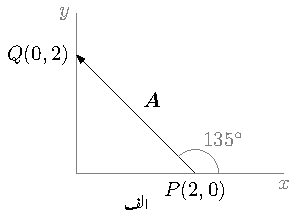
\includegraphics{figVectorVectorInCartesianAndCylindricalA}
\end{subfigure}%
%
\begin{subfigure}{0.5\textwidth}
\centering
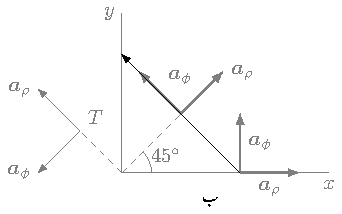
\includegraphics{figVectorVectorInCartesianAndCylindricalB}
\end{subfigure}%
\caption{کارتیسی اور نلکی محدد میں سمتیہ۔}
\label{شکل_سمتیہ_کارتیسی_نلکی_مساوات}
\end{figure}

شکل \حوالہ{شکل_سمتیہ_کارتیسی_نلکی_مساوات} میں \عددیء{P(2,0)} سے \عددیء{Q(0,2)} تک سمتیہ \عددیء{\kvec{A}} دکھایا گیا ہے۔کارتیسی نظام میں 
\begin{align}\label{مساوات_سمتیہ_کارتیسی_نظام_سمتیہ_مثال}
\kvec{A}&=-2\ax+2\ay
\end{align}
لکھا جا سکتا ہے۔اس سمتیہ کی حتمی قیمت
\begin{align*}
\abs{\kvec{A}}= \sqrt{\kvec{A} \cdot \kvec{A}}=\sqrt{(-2\ax+2\ay) \cdot (-2\ax+2\ay)}=\sqrt{8}
\end{align*}
ہے۔آئیں اسی سمتیہ کو نلکی محدد میں لکھیں۔ایسا کرنے کی خاطر \عددیء{A_\rho} اور \عددیء{A_\phi} درکار ہوں گے جنہیں حاصل کرنے کی خاطر جدول \حوالہ{جدول_سمتیہ_نلکی_کارتیسی_اکائی_غیر-سمتی_ضرب}  کی مدد سے \عددیء{\arho \cdot \kvec{A}} اور \عددیء{\aphi \cdot \kvec{A}} حاصل کرتے ہیں۔
\begin{align*}
A_\rho&=\arho \cdot (-2\ax+2\ay)=-2 \cos \phi +2 \sin \phi\\
A_\phi&=\aphi \cdot  (-2\ax+2\ay)=2 \sin \phi +2 \cos \phi
\end{align*}
یوں
\begin{align}\label{مساوات_سمتیہ_نلکی_نظام_سمتیہ_مثال}
\kvec{A}=2(- \cos \phi + \sin \phi) \arho +2( \sin \phi + \cos \phi)\aphi
\end{align}
لکھا جا سکتا ہے۔آئیں دیکھیں کہ اس کی حتمی قیمت کیا حاصل ہوتی ہے۔اکائی سمتیات کا غیر سمتی ضرب \عددیء{\arho \cdot \arho=1}، \عددیء{\aphi \cdot \aphi=1} اور \عددیء{\arho \cdot \aphi=0} استعمال کرتے ہوئے
\begin{align*}
\abs{\kvec{A}}&=\sqrt{\kvec{A} \cdot \kvec{A}}\\
&=\sqrt{2^2(- \cos \phi + \sin \phi)^2+2^2( \sin \phi + \cos \phi)^2 }\\
&=\sqrt{4(\cos^2 \phi +\sin^2 \phi -2 \cos \phi \sin \phi)+4(\cos^2 \phi +\sin^2 \phi +2 \cos \phi \sin \phi)}\\
&=\sqrt{8(\cos^2 \phi+\sin^2 \phi)}\\
&=\sqrt{8}
\end{align*}
حاصل ہوتا ہے جہاں آخری قدم پر \عددیء{\cos^2 \alpha+\sin^2 \alpha=1} کا استعمال کیا گیا ہے۔یقیناً سمتیہ کی حتمی قیمت محدد کے نظام پر منحصر نہیں۔

مساوات \حوالہ{مساوات_سمتیہ_کارتیسی_نظام_سمتیہ_مثال} اور مساوات \حوالہ{مساوات_سمتیہ_نلکی_نظام_سمتیہ_مثال} ایک ہی سمتیہ کو لکھنے کے دو طریقے ہیں۔یہاں کارتیسی نظام کا استعمال نہایت آسان ثابت ہوا۔ آگے چل کر آپ دیکھیں گے کہ کہیں مسئلوں میں نلکی محدد کا استعمال زیادہ آسان ہو گا۔آئیں مساوات \حوالہ{مساوات_سمتیہ_کارتیسی_نظام_سمتیہ_مثال} پر مزید غور کریں۔اس مساوات میں اکائی سمتیات از خود اٹل نہیں ہیں۔ان کی سمتوں کا دارومدار زاویہ \عددیء{\phi} پر ہے۔شکل  \حوالہ{شکل_سمتیہ_کارتیسی_نلکی_مساوات}-ب میں \عددیء{\phi=0^\circ}، \عددیء{\phi=45^\circ} اور \عددیء{\phi=135^\circ} پر \عددیء{\arho} اور \عددیء{\aphi} دکھائے گئے ہیں۔نقطہ \عددیء{P} یعنی \عددیء{\phi=0^\circ} پر مساوات \حوالہ{مساوات_سمتیہ_نلکی_نظام_سمتیہ_مثال} 
\begin{align*}
\kvec{A}_{ \phi=0^\circ}&=2(- \cos 0^\circ + \sin 0^\circ ) \arho +2( \sin 0^\circ  + \cos 0^\circ )\aphi\\
&=-2\arho+2\aphi 
\end{align*} 
صورت اختیار کر لیتی ہے۔اس مساوات کے مطابق \عددیء{\phi=0^\circ} پر \عددیء{\kvec{A}} کو دو عدد سمتیات کے مجموعہ کی صورت میں لکھا جا سکتا ہے جن میں پہلی سمتیہ \عددیء{\arho} کے الٹ سمت میں ہے اور اس کی لمبائی دو کے برابر ہے جبکہ دوسری سمتیہ کی مقدار دو اور اس کی سمت \عددیء{\aphi} کی سمت میں ہی ہے۔\حوالہ{شکل_سمتیہ_کارتیسی_نلکی_مساوات}-ب میں نقطہ \عددیء{P} پر \عددیء{\kvec{A}} کی سمت واقع بڑھتی \عددیء{\aphi} اور گھٹتی \عددیء{\arho} کی سمت میں ہے۔یاد رہے کہ اس مساوات میں \عددیء{\arho} اور \عددیء{\aphi} کو \عددیء{\phi=0^\circ} پر حاصل کیا گیا ہے۔\عددیء{\phi=0^\circ} پر \عددیء{\arho} اور \عددیء{\ax} برابر ہوتے ہیں اور اسی طرح \عددیء{\aphi} اور \عددیء{\ay} برابر ہوتے ہیں۔یہی وجہ ہے کہ مساوات \حوالہ{مساوات_سمتیہ_کارتیسی_نظام_سمتیہ_مثال} میں \عددیء{\ax} کی جگہ \عددیء{\arho} اور \عددیء{\ay} کی جگہ \عددیء{\aphi} پُر کرنے سے مندرجہ بالا مساوات لکھی جا سکتی ہے۔

\عددیء{\phi=45^\circ} پر مساوات \حوالہ{مساوات_سمتیہ_نلکی_نظام_سمتیہ_مثال}
\begin{align*}
\kvec{A}_{\phi=45^\circ}&=2(- \cos 45^\circ + \sin 45^\circ ) \arho +2( \sin 45^\circ  + \cos 45^\circ )\aphi\\
&=2(- \frac{1}{\sqrt{2}} +\frac{1}{\sqrt{2}} ) \arho +2( \frac{1}{\sqrt{2}}  + \frac{1}{\sqrt{2}} )\aphi\\
&=\sqrt{8} \aphi
\end{align*} 
صورت اختیار کر لیتی ہے۔اس مساوات کے مطابق \عددیء{\phi=45^\circ} پر \عددیء{\kvec{A}} صرف اور صرف \عددیء{\aphi} کی سمت میں ہے اور اس کی لمبائی \عددیء{\sqrt{8}} ہے۔شکل \حوالہ{شکل_سمتیہ_کارتیسی_نلکی_مساوات}-ب میں یہ حقیقت واضح ہے کہ \عددیء{\phi=45^\circ}  پر \عددیء{\kvec{A}} کی سمت \عددیء{\aphi} ہی ہے۔یاد رہے کہ اس مساوات میں \عددیء{\arho} اور \عددیء{\aphi} کو \عددیء{\phi=45^\circ} پر حاصل کیا گیا ہے۔شکل میں اکائی سمتیات کو عین \عددیء{\kvec{A}} کے اوپر کھینچا گیا ہے تا کہ سمتیات کی سمتوں کا موازنہ آسانی سے کیا جا سکے۔

آپ نے دیکھا کہ نلکی محدد میں سمتیہ کی مساوات کا دارومدار اس نقطے پر ہے جس نقطے کے اکائی سمتیات استعمال کئے جائیں۔آئیں دیکھیں کہ \عددیء{\phi=135^\circ} پر پائے جانے والے  نقطہ \عددیء{T} کے اکائی سمتیات استعمال کرتے ہوئے \عددیء{\kvec{A}} کیسا لکھا جائے گا۔مساوات \حوالہ{مساوات_سمتیہ_نلکی_نظام_سمتیہ_مثال} میں \عددیء{\phi=135^\circ} پُر کرنے سے
\begin{align*}
\kvec{A}_{\phi=135^\circ}&=2(- \cos 135^\circ + \sin 135^\circ) \arho +2( \sin 135^\circ + \cos 135^\circ)\aphi\\
&=2(\frac{1}{\sqrt{2}}+\frac{1}{\sqrt{2}})\arho+2(\frac{1}{\sqrt{2}}-\frac{1}{\sqrt{2}})\aphi\\
&=\sqrt{8}\arho
\end{align*}
حاصل ہوتا ہے۔اس مساوات کے مطابق \عددیء{\phi=135^\circ} کے اکائی سمتیات استعمال کرتے ہوئے \عددیء{\kvec{A}} کو \عددیء{\arho} کی سمت میں \عددیء{\sqrt{8}} لمبائی کا سمتیہ لکھا جا سکتا ہے۔شکل سے یہ حقیقت واضح ہے۔ 

\begin{figure}
\centering
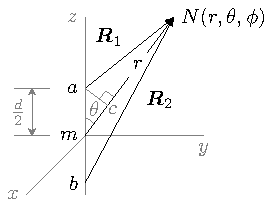
\includegraphics{figVectorDipole}
\caption{جفت قطب کے برقی بار سے دور نقطے تک فاصلے۔}
\label{شکل_سمتیہ_جفت_قطب}
\end{figure}
%================
\ابتدا{مثال}\شناخت{مثال_سمتیہ_جفت_قطب}
شکل \حوالہ{شکل_سمتیہ_جفت_قطب} میں \عددیء{z} محدد پر نقطہ \عددیء{a(0,0,\tfrac{d}{2})} پر مثبت \اصطلاح{برقی بار}\فرہنگ{برقی بار}\فرہنگ{بار!برقی}\فرہنگ{برق}\حاشیہب{electric charge}\فرہنگ{charge} \عددیء{+Q} اور نقطہ \عددیء{b(0,0,-\tfrac{d}{2})} پر منفی برقی بار  \عددیء{-Q} پائے جاتے ہیں۔ایسے دو برابر لیکن الٹ علامت کے دو قریب قریب پائے جانے والے برقی باروں کے جوڑی کو \اصطلاح{جفت قطب}\فرہنگ{جفت قطب}\حاشیہب{dipole}\فرہنگ{dipole} کہتے ہیں۔دکھائے گئے سمتی فاصلوں \عددیء{\kvec{R}_1} اور \عددیء{\kvec{R}_2} کو کروی محدد میں لکھیں۔ 

حل:\عددیء{m} سے \عددیء{N} تک فاصلہ \عددیء{r} ہے اور اس سمت میں اکائی سمتیہ \عددیء{\ar} ہے۔نقطہ \عددیء{a} سے  \عددیء{r} پر عمودی لکیر لگائی گئی ہے جو اسے \عددیء{c} پر ملتی ہے۔یوں \عددیء{ac} کی سمت کروی محدد کے اکائی سمتیہ \عددیء{\atheta} کی سمت میں ہے۔شکل کو دیکھتے ہوئے \عددیء{mc=\tfrac{d}{2} \cos \theta} اور \عددیء{ac=\tfrac{d}{2} \sin \theta} لکھے جا سکتے ہیں۔یوں \عددیء{\kvec{R}_1} کو ہم \عددیء{a} سے \عددیء{c} تک سمتیہ \عددیء{\tfrac{d}{2} \sin \theta \atheta} اور \عددیء{c} سے \عددیء{N} تک سمتیہ \عددیء{(r-\tfrac{d}{2}\cos \theta)\ar} کے مجموعے کی شکل میں 
\begin{align}
\kvec{R}_1=\frac{d}{2}\sin\theta \atheta+(r-\frac{d}{2}\cos\theta)\ar
\end{align}
 لکھ سکتے ہیں۔ہم اسی طرح شکل \حوالہ{شکل_سمتیہ_جفت_قطب} میں \عددیء{N} سے \عددیء{m} تک لکیر کو \عددیء{m} سے آگے بڑھا کر \عددیء{b} سے اس پر عمودی لکیر کھینچ کر شکل کو دیکھتے ہوئے  \عددیء{\kvec{R}_2} کی مساوات بھی لکھ سکتے ہیں البتہ ایسا کرنے کی بجائے آئیں \عددیء{\kvec{R}_2} کی مساوات تحلیلی طریقے سے حاصل کریں۔شکل کو دیکھتے ہوئے
\begin{align*}
\kvec{R}_2=\frac{d}{2} \az+r\ar
\end{align*}
لکھا جا سکتا ہے جہاں کارتیسی محدد کی اکائی سمتیہ \عددیء{\az} اور کروی محدد کی اکائی سمتیہ \عددیء{\ar} استعمال کئے گئے۔کروی محدد میں کسی بھی لکیر کی طرح 
\begin{align*}
\kvec{R}_2=A_r \ar+A_\theta \atheta+A_\phi \aphi
\end{align*}
لکھا جا سکتا ہے۔آئیں \عددیء{A_r=\kvec{R}_2 \cdot \ar} سے حاصل کریں۔
\begin{align*}
A_r =\left(\frac{d}{2} \az+r\ar \right) \cdot \ar=\frac{d}{2}\cos \theta+r
\end{align*}
اسی طرح \عددیء{A_\theta=\kvec{R}_2 \cdot \atheta} سے حاصل کرتے ہیں۔
\begin{align*}
A_\theta =\left(\frac{d}{2} \az+r\ar \right) \cdot \atheta=-\frac{d}{2}\sin \theta
\end{align*}
اسی طرح \عددیء{A_\phi=\kvec{R}_2 \cdot \aphi} لکھتے ہوئے \عددیء{A_\phi=0} حاصل ہوتا ہے۔یوں
\begin{align}
\kvec{R}_2=\left(\frac{d}{2}\cos \theta+r \right)\ar-\frac{d}{2}\sin \theta \atheta
\end{align}
لکھا جا سکتا ہے۔
\انتہا{مثال}
%
\begin{figure}
\centering
\begin{subfigure}{0.5\textwidth}
\centering
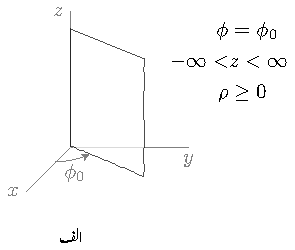
\includegraphics{figVectorCylindricalFixedAngleSurface}
\end{subfigure}%
%
\begin{subfigure}{0.5\textwidth}
\centering
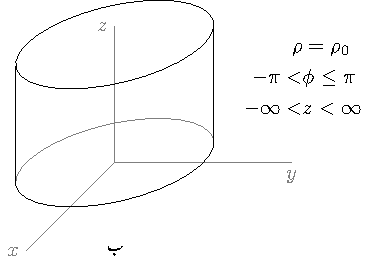
\includegraphics[scale=0.95]{figVectorCylindricalFixedRadiusSurface}
\end{subfigure}%
\caption{$\phi=\phi_0$ اور $\rho=\rho_0$ سطحیں۔}
\label{شکل_سمتیہ_نلکی_قطعی_زاویہ_سطح}
\end{figure}
\جزوحصہ{نلکی لامحدود سطحیں}
شکل \حوالہ{شکل_سمتیہ_نلکی_قطعی_زاویہ_سطح}-الف میں \عددیء{\phi} تبدیل کئے بغیر \عددیء{\rho} اور \عددیء{z} کی قیمتیں تبدیل کرتے ہوئے \عددیء{\phi=\phi_0} سطح کا حصول دکھایا گیا ہے۔یہ سطح نلکی شکل رکھتی ہے  جس کا اوپر والا منہ اور نچلا منہ کھلے ہیں یعنی ان پر ڈھکن نہیں۔شکل-ب میں \عددیء{\rho} تبدیل کئے بغیر \عددیء{\phi} اور \عددیء{z} کو تبدیل کرتے ہوئے \عددیء{\rho=\rho_0} سطح کا حصول دکھایا گیا ہے۔ان دونوں لامحدود سطحوں کے کچھ حصے ان  اشکال میں  دکھائے گئے ہیں۔ شکل-الف میں \عددیء{\rho} کی قیمت صرف مثبت جبکہ \عددیء{z} کی قیمت مثبت یا منفی ممکن ہے۔شکل-ب میں زاویہ کُل \عددیء{2\pi} ریڈیئن تبدیل ہو سکتا ہے۔یوں زاویے کا مثبت حد \عددیء{\pi} ریڈیئن یعنی \عددیء{180} درجہ ہے جبکہ اس کا منفی\حاشیہد{حقیقت میں منفی حد \عددیء{-180^\circ} کو نہیں چھوتا۔اگر منفی حد \عددیء{-180^\circ} کو چھوئے تب منفی \عددیء{x} محدد دو مرتبہ شامل ہوتا ہے۔} حد \عددیء{-\pi} یعنی \عددیء{-180} درجے ہے۔نلکی محدد اور کارتیسی نظام دونوں میں \عددیء{z=z_0}  سطح یکساں بنتی ہے۔

جیسے شکل \حوالہ{شکل_سمتیہ_نلکی_تین_سطحیں} میں دکھایا گیا ہے، \عددیء{\rho=\rho_1} اور \عددیء{\phi=\phi_1}  سطحیں \عددیء{\az} کی سیدھ میں سیدھی لکیر پر ملتے ہیں۔اسی طرح \عددیء{\rho=\rho_1} اور \عددیء{z=z_1} سطحیں ایک گول دائرے پر ملتے ہیں جبکہ \عددیء{\phi=\phi_1} اور \عددیء{z=z_1} سطحیں \عددیء{\arho} کی سیدھ میں سیدھی لکیر پر ملتے ہیں۔\عددیء{\rho=\rho_1}، \عددیء{\phi=\phi_1} اور \عددیء{z=z_1} سطحیں صرف اور صرف ایک ہی نقطہ \عددیء{N} پر اکٹھے ملتے ہیں۔نلکی محدد میں کسی بھی نقطے  کا مقام اسی طرح تین سطحوں کے  متقاطع نقطہ سے حاصل کیا جاتا ہے البتہ \عددیء{(0,0,z)} تک پہنچنے کی خاطر ایسا کرنے کی ضرورت نہیں ہوتی۔

\begin{figure}
\centering
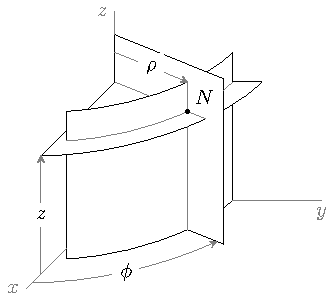
\includegraphics{figVectorCylindricalIntersectingSurfaces}
\caption{نلکی محدد کے تین سطحیں۔}
\label{شکل_سمتیہ_نلکی_تین_سطحیں}
\end{figure}
کسی بھی نقطہ \عددیء{N(\rho_1,\phi_1,z_1)} پر \عددیء{\rho=\rho_1}، \عددیء{\phi=\phi_1} اور \عددیء{z=z_1} سطحیں  بنانے کے بعد اگر نلکی محدد کے متغیرات کو \عددیء{\dif \rho}، \عددیء{\dif \phi} اور \عددیء{\dif z} بڑھا کر مزید تین سطحیں کھینچے جائیں تو یہ چھ سطحیں مل کر منحرف مکعب نما\حاشیہد{چھوٹے مکعب نما کو اس کتاب میں مکعب ہی کہا جائے گا۔} کو گھیریں گے جسے شکل \حوالہ{شکل_سمتیہ_نلکی_چھوٹی_حجم}-الف میں دکھایا گیا ہے۔رداسی سمت میں اس منحرف مکعب کے اطراف کی لمبائی \عددیء{\dif \rho} جبکہ \عددیء{\az}  سمت کے اطراف کی لمبائی \عددیء{\dif z} ہے۔ \عددیء{\aphi} سمت میں \عددیء{z} محدد کے قریبی  گول طرف کی لمبائی \عددیء{\rho \dif \phi} جبکہ محدد سے دور طرف کی گول لمبائی \عددیء{(\rho+\dif \rho)\dif \phi} ہے۔جیسے جیسے اس منحرف مکعب کو چھوٹا کیا جائے ویسے ویسے یہ ایک درست مکعب کی صورت اختیار کرتا ہے لہٰذا نہایت چھوٹے حجم کو مکعب تصور کرتے ہوئے اس کا حجم \عددیء{\rho \dif \rho \dif \phi \dif z} لکھا جا سکتا ہے۔
\begin{figure}
\centering
\begin{subfigure}{0.5\textwidth}
\centering
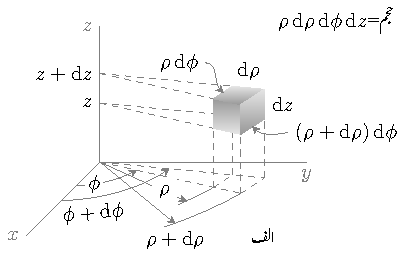
\includegraphics[scale=0.9]{figVectorCylindricalDifferentialVolume}
\end{subfigure}%
%
\begin{subfigure}{0.5\textwidth}
\centering
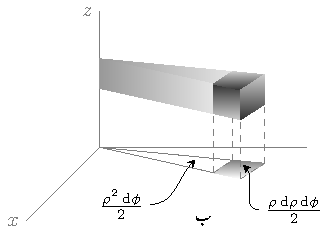
\includegraphics{figVectorCylindricalDifferentialTrapezium}
\end{subfigure}%
\caption{نلکی محدد میں انتہائی چھوٹی حجم۔}
\label{شکل_سمتیہ_نلکی_چھوٹی_حجم}
\end{figure}  

شکل \حوالہ{شکل_سمتیہ_نلکی_چھوٹی_حجم}-ب میں چھوٹے منحرف مکعب کو رداسی سمت میں \عددیء{z} محدد تک بڑھا کر پچر یا فانہ کی شکل میں دکھایا گیا ہے۔\عددیء{z=0} سطح پر اس کا عمودی سایہ بھی دکھایا گیا ہے۔\عددیء{\rho} رداس کے گول دائرے  کے مرکز سے  \عددیء{\dif \phi} زاویے پر دو لکیریں دائرے تک کھینچنے سے  \عددیء{\tfrac{\rho^2 \dif \phi}{2}} رقبہ گھیرا جاتا ہے۔اگر رداس \عددیء{\rho+\dif \rho} ہو تب رقبہ \عددیء{\tfrac{(\rho+\dif \rho)^2 \dif \phi}{2}} ہو گا۔یوں شکل-ب میں چھوٹے مکعب کے سایہ  کا رقبہ \عددیء{\dif S}
\begin{align*}
\dif S&=\frac{(\rho+\dif \rho)^2 \dif \phi}{2} - \frac{\rho^2 \dif \phi}{2}\\
&=\frac{\rho^2 \dif \phi +2 \rho \dif \rho \dif \phi+(\dif \rho)^2 \dif \phi}{2}-\frac{\rho^2 \dif \phi}{2}\\
&=\rho \dif \rho \dif \phi+\frac{(\dif \rho)^2 \dif \phi}{2}\\
&\approx \rho \dif \rho \dif \phi
\end{align*}
ہو گا۔یہاں آخری قدم پر \عددیء{\dif} کی علامت، مجموعہ کے پہلے رکن میں دو مرتبہ  جبکہ دوسرے رکن میں تین مرتبہ ہے۔یوں دوسرے اور پہلے رکن کی نسبت
  \عددیء{\tfrac{0.5(\dif \rho)^2 \dif \phi}{\rho \dif \rho \dif \phi}=\tfrac{\dif \rho}{2\rho}} ہو گی۔\عددیء{\dif \rho} کو کم سے کم\حاشیہد{کسی بھی متغیرہ مثلاً \عددیء{\rho} میں چھوٹی سی تبدیلی کو \عددیء{\Delta \rho} لکھا جاتا ہے جبکہ اس میں کم سے کم تبدیلی کو \عددیء{\dif \rho} لکھا 
جاتا ہے۔\عددیء{\dif \rho} کو تقریباً صفر سمجھا جا سکتا ہے یعنی \عددیء{\dif \rho \to 0} ہوتا ہے۔} کرتے ہوئے دوسرے رکن کو قابل نظر انداز بناتے ہوئے نظرانداز کیا گیا ہے۔یوں \عددیء{\rho \dif \rho \dif \phi} رقبہ اور \عددیء{\dif z} بلندی کے مکعب کا حجم \عددیء{\rho \dif \rho \dif \phi \dif z} ہو گا۔

شکل \حوالہ{شکل_سمتیہ_نلکی_چھوٹی_حجم} کو درست مکعب تصور کرتے ہوئے، اس کے اطراف کی لمبائی \عددیء{\rho \dif \phi}، \عددیء{\dif \rho} اور \عددیء{\dif z} لی جاتی ہے۔یوں مکعب کے نچلی اور اوپر سطح کا رقبہ مستطیل کے اطراف کو ضرب دیتے ہوئے  \عددیء{\rho \dif \rho \dif \phi} لکھا جا سکتا ہے۔اسی طرح سامنے اور پیچھے سطحوں  کا رقبہ \عددیء{\dif \rho \dif z} جبکہ بائیں اور دائیں سطحوں کا رقبہ \عددیء{\rho \dif \phi \dif z} لکھا جا سکتا ہے۔


شکل \حوالہ{شکل_سمتیہ_نلکی_چھوٹی_حجم}-الف میں نلکی محدد کے تینوں متغیرات تبدیل کرتے ہوئے ہم چھوٹے مکعب کے  \عددیء{N(\rho, \phi,z)} کونے سے \عددیء{N'(\rho+\dif \rho,\phi+\dif \phi,z+\dif z)} کونے پہنچتے ہیں۔\عددیء{N} سے \عددیء{N'} تک سمتیہ کو
\begin{align}\label{مساوات_سمتیہ_نلکی_چھوٹا_فاصلہ}
\dif \kvec{L}=\dif \rho \arho+\rho \dif \phi \aphi+\dif z \az
\end{align}
لکھا جاتا ہے۔یہ مساوات کسی بھی دو قریبی نقطوں کے مابین سمتی فاصلے کو ظاہر کرتی ہے۔

\حصہ{کروی محدد}
سیدھی لکیروں اور سیدھی سطحوں کو کارتیسی محدد میں زیادہ آسانی سے ظاہر کیا جا سکتا ہے جبکہ نلکی سطحوں کو ظاہر کرنے کے لئے نلکی محدد بہتر ثابت ہوتا ہے۔اسی طرح کروی اشکال کے سطحوں کو کروی محدد میں باآسانی لکھا جا سکتا ہے۔آئیں کروی نظام پر غور کریں۔

شکل \حوالہ{شکل_سمتیہ_کروی_محدد_متغیرات}-الف میں کروی محدد کے متغیرات \عددیء{r}، \عددیء{\theta} اور \عددیء{\phi} دکھائے گئے ہیں۔محدد کے مرکز سے نقطہ \عددیء{N} تک کے فاصلے \عددیء{r} کو کروی رداس پکارا جاتا ہے جبکہ \عددیء{z} محدد سے کروی رداس تک زاویے کو \عددیء{\theta} لکھا جاتا ہے۔\عددیء{x} محدد سے رداس کے عمودی سائے تک زاویہ \عددیء{\phi} ہے۔کروی اور نلکی نظام میں \عددیء{\phi} یکساں بیان کیا جاتا ہے۔رداس کی  قیمت مثبت لی جاتی ہے۔یوں \عددیء{r \ge 0} ممکن ہے۔\عددیء{\theta} کی کم سے کم قیمت \عددیء{0^\circ} اور  زیادہ سے زیادہ  قیمت \عددیء{180^\circ} ہے جبکہ \عددیء{\phi} کی کم سے کم قیمت \عددیء{0^\circ} اور زیادہ سے زیادہ قیمت \عددیء{360^\circ} ہے۔

\begin{figure}
\centering
\begin{subfigure}{0.5\textwidth}
\centering
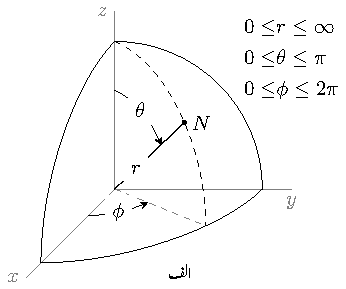
\includegraphics{figVectorSphericalRadiusThetaPhi}
\end{subfigure}%
%
\begin{subfigure}{0.5\textwidth}
\centering
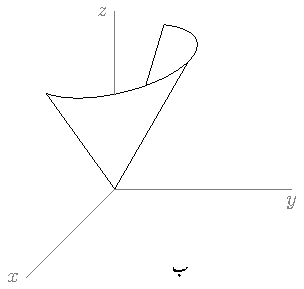
\includegraphics{figVectorSphericalThetaSurface}
\end{subfigure}%
\caption{(الف) کروی محدد کے متغیرات۔ (ب) \عددیء{\theta=\theta_0} سطح  کا کچھ حصہ۔}
\label{شکل_سمتیہ_کروی_محدد_متغیرات}
\end{figure}
%
\عددیء{r} اور \عددیء{\phi} تبدیل کئے بغیر \عددیء{\theta} کو \عددیء{0} سے بڑھاتے ہوئے \عددیء{\pi} ریڈیئن  کرنے سے نقطہ \عددیء{N}  شکل \حوالہ{شکل_سمتیہ_کروی_محدد_متغیرات}-الف میں نقطہ دار لکیر پر چلتے ہوئے  مثبت \عددیء{z} محدد سے شروع ہو کر  منفی \عددیء{z} محدد پر پہنچتا ہے۔اسے  نقطہ دار لکیر کو  کرہ ارض کے \اصطلاح{خط طول بلد}\فرہنگ{خط!طول بلد}\حاشیہب{longitude}\فرہنگ{longitude} تصور  کیا جا سکتا ہے۔  شکل-الف میں \عددیء{\theta} کا \عددیء{0^\circ} تا \عددیء{90^\circ} تبدیل ہوتا دکھایا گیا ہے۔اسی طرح \عددیء{r} اور \عددیء{\theta} تبدیل کئے بغیر \عددیء{\phi} کو \عددیء{0^\circ} تا \عددیء{360^\circ} تبدیل کرنے سے  نقطہ \عددیء{N} گول دائرے پر \عددیء{z} محدد کے گرد ایک چکر کاٹے گا۔یہ حرکت کرہ ارض کے \اصطلاح{خط عرض بلد}\فرہنگ{خط!عرض بلد}\حاشیہب{latitude}\فرہنگ{latitude} پر چلنے کے  مانند ہے۔\عددیء{\theta} اور \عددیء{\phi} تبدیل کئے بغیر \عددیء{r} کو تبدیل کرنے سے نقطہ \عددیء{N} مرکز سے  سیدھی باہر نکلتی لکیر پر حرکت کرتا ہے۔ 

\begin{figure}
\centering
\begin{subfigure}{0.5\textwidth}
\centering
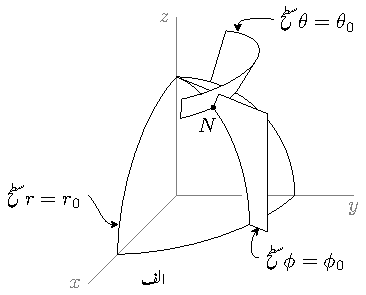
\includegraphics[scale=0.95]{figVectorSphericalIntersectingSurface}
\end{subfigure}%
%
\begin{subfigure}{0.5\textwidth}
\centering
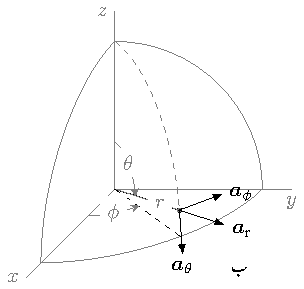
\includegraphics{figVectorSphericalUnitVectors}
\end{subfigure}%
\caption{(الف) تین عمودی سطحوں کے ملاپ سے نقطہ \عددیء{N} کا حصول۔ (ب) کروی محدد کے تین عمودی اکائی سمتیات۔}
\label{شکل_سمتیہ_کروی_تین_سطحوں_کا_ملاپ}
\end{figure}

\عددیء{r} تبدیل کئے بغیر \عددیء{\theta} کو \عددیء{0^\circ} تا \عددیء{180^\circ} اور \عددیء{\phi} کو \عددیء{0^\circ} تا \عددیء{360^\circ} تبدیل کرنے سے  نقطہ \عددیء{N} کروی \عددیء{r=r_0} سطح  پر حرکت کرے گا۔ اس کروی سطح کا رداس \عددیء{r} ہو گا۔شکل \حوالہ{شکل_سمتیہ_کروی_محدد_متغیرات}-الف  میں \عددیء{\theta} کو \عددیء{0^\circ} تا \عددیء{90^\circ} اور \عددیء{\phi} کو \عددیء{0^\circ} تا \عددیء{90^\circ} تبدیل کرنے سے حاصل سطح  دکھائی گئی ہے۔شکل \حوالہ{شکل_سمتیہ_کروی_محدد_متغیرات}-ب میں \عددیء{\theta} تبدیل کئے بغیر \عددیء{r} اور \عددیء{\phi} تبدیل کرنے سے پیدا مخروط\فرہنگ{مخروط}\حاشیہب{cone}\فرہنگ{cone}  \عددیء{\theta=\theta_0}  کروی سطح دکھائی گئی ہے۔\عددیء{\phi} تبدیل کئے بغیر \عددیء{r} اور \عددیء{\theta} تبدیل کرنے سے  نلکی محدد کی طرح \عددیء{\phi=\phi_0} سطح حاصل ہوتی ہے۔ شکل \حوالہ{شکل_سمتیہ_کروی_تین_سطحوں_کا_ملاپ}-الف میں ان تینوں سطحوں کو دکھایا گیا ہے۔بالکل کارتیسی اور نلکی محدد کی طرح، کسی بھی نقطہ \عددیء{N(r_0,\theta_0,\phi_0)} کا مقام ان تین سطحوں کے نقطہ ملاپ سے اخذ کیا جاتا ہے۔کسی بھی نقطہ \عددیء{N(r_0,\theta_0,\phi_0)} پر \عددیء{r=r_0}، \عددیء{\theta=\theta_0} اور \عددیء{\phi=\phi_0} سطحیں آپس میں عمودی ہوتی ہے اور یہ صرف اور صرف اسی نقطے پر اکٹھے ملتی ہیں۔

شکل \حوالہ{شکل_سمتیہ_کروی_تین_سطحوں_کا_ملاپ}-ب میں کروی نظام کے تین عمودی اکائی سمتیات \عددیء{\ar}، \عددیء{\atheta} اور \عددیء{\aphi} دکھائے گئے ہیں۔نلکی محدد کی طرح کروی محدد کے عمودی اکائی سمتیات بھی مقام تبدیل کرنے سے تبدیل ہوتے ہیں۔کسی بھی نقطہ \عددیء{N(r_0,\theta_0,\phi_0)} پر \عددیء{\theta} اور \عددیء{\phi} تبدیل کئے بغیر \عددیء{r} کے بڑھتے جانب اکائی سمتیہ \عددیء{\ar} ہو گی۔اسی طرح \عددیء{\theta} بڑھانے سے نقطہ \عددیء{N} اکائی سمتیہ \عددیء{\atheta} کی جانب حرکت کرے گا جبکہ \عددیء{\phi} بڑھانے سے نقطہ \عددیء{\aphi} کی جانب حرکت کرے گا۔کارتیسی اور نلکی محدد کی طرح کروی محدد کے اکائی سمتیات کو بھی محددی نظام کے متغیرات کو کم سے کم بڑھاتے ہوئے  نقطے کی حرکت کی جانب اکائی سمتیہ کھینچنے سے حاصل کیا جاتا ہے۔

شکل \حوالہ{شکل_سمتیہ_کروی_تین_سطحوں_کا_ملاپ}-الف سے واضح ہے کہ \عددیء{\ar} سمتیہ \عددیء{r=r_0} سطح کے عمودی جبکہ \عددیء{\theta=\theta_0} اور \عددیء{\phi=\phi_0} سطحوں کے متوازی ہے۔اسی طرح \عددیء{\atheta} سمتیہ \عددیء{\theta=\theta_0} سطح کے عمودی اور \عددیء{\phi=\phi_0} سطح کے متوازی پایا جاتا ہے جبکہ \عددیء{r=r_0} سطح کے ساتھ مماس بناتا ہے۔\عددیء{\aphi} سمتیہ \عددیء{\phi=\phi_0} سطح کے عمودی جبکہ \عددیء{r=r_0} اور \عددیء{\theta=\theta_0} سطحوں کے ساتھ مماس بناتا ہے۔

 
\عددیء{\ar}، \عددیء{\atheta} اور \عددیء{\aphi} کروی نظام  کے اکائی سمتیات ہیں۔\عددیء{\ar \times \atheta=\aphi} لکھنے سے  دائیں ہاتھ کا کروی نظام حاصل ہوتا ہے۔دائیں ہاتھ کے قانون میں دائیں ہاتھ کا انگوٹھا  \عددیء{r} جبکہ پہلی انگلی \عددیء{\theta}  اور دوسری انگلی \عددیء{\phi} بڑھانے سے پیدا حرکت کی سمتوں کو ظاہر کرتے ہیں۔نلکی محدد میں یہ انگلیاں \عددیء{\rho}، \عددیء{\phi} اور \عددیء{z} جبکہ کارتیسی محدد میں \عددیء{x}، \عددیء{y} اور \عددیء{z} بڑھانے سے پیدا حرکت کی سمتوں کو ظاہر کرتی ہیں۔

دائیں ہاتھ کے قانون  یا شکل \حوالہ{شکل_سمتیہ_کروی_صلیبی_ضرب_اکائی_سمتیات} کی مدد سے یوں اکائی سمتیات کے صلیبی ضرب
\begin{figure}
\centering
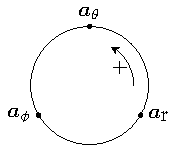
\includegraphics{figVectorSphericalRightHandCircle}
\caption{کروی نظام میں اکائی سمتیات کی صلیبی ضرب۔}
\label{شکل_سمتیہ_کروی_صلیبی_ضرب_اکائی_سمتیات}
\end{figure}

\begin{align}
\ar \times \atheta=\aphi \,\, , \quad \atheta \times \aphi=\ar \, \, , \quad \aphi \times \ar =\atheta
\end{align}

لکھے جا سکتے ہیں۔اسی طرح
\begin{align}
\ar \cdot \ar=1 \,\, , \quad \atheta \cdot \atheta=1 \,\, , \quad \aphi \cdot \aphi=1
\end{align}
اور
\begin{align}
\ar \cdot \atheta=0 \,\, , \quad \atheta \cdot \aphi=0 \,\, , \quad \aphi \cdot \ar=0
\end{align}
بھی لکھے جا سکتے ہیں۔

\begin{figure}
\centering
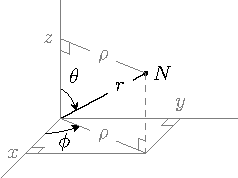
\includegraphics{figVectorSphericalToCylindricalAndCartesian}
\caption{کروی، نلکی اور کارتیسی متغیرات کا تبادلہ۔}
\label{شکل_سمتیہ_کروی_نلکی_متغیرات_تبادلہ}
\end{figure}

نقطہ \عددیء{N} کا \عددیء{z} محدد سے فاصلہ  \عددیء{\rho} ہے جو نلکی محدد کا رداس ہے۔اسے شکل \حوالہ{شکل_سمتیہ_کروی_نلکی_متغیرات_تبادلہ} میں دکھایا گیا ہے جہاں سے واضح ہے کہ \عددیء{\rho=r \sin \theta} کے برابر ہے۔اسی طرح \عددیء{z=0} سطح سے \عددیء{N} کی اونچائی \عددیء{z} ہے جو شکل کو دیکھتے ہوئے \عددیء{z=r\cos \theta}  لکھی جا سکتی ہے۔نقطہ \عددیء{N} کا عمودی سایہ \عددیء{z=0} سطح پر دکھایا گیا ہے جہاں سے واضح ہے کہ \عددیء{x=\rho \cos \phi} اور \عددیء{y=\rho \sin \phi} لکھے جا سکتے ہیں۔\عددیء{\rho=r \sin \theta} پُر کرنے سے درج ذیل لکھے جا سکتے ہیں
\begin{gather}
\begin{aligned}\label{مساوات_سمتیہ_کروی_سے_کارتیسی}
x&=r \sin \theta \cos \phi\\
y&=r \sin \theta \sin \phi\\
z&=r \cos \theta
\end{aligned}
\end{gather}
جہاں \عددیء{z} کی مساوات بھی ساتھ ہی لکھی  گئی ہے۔مساوات \حوالہ{مساوات_سمتیہ_کروی_سے_کارتیسی} کروی سے کارتیسی متغیرات دیتا ہے۔ اسی شکل کو دیکھتے ہوئے مسئلہ فیثاغورث کی مدد سے 
\begin{gather}
\begin{aligned}
r^2&=\rho^2+z^2\\
\rho^2&=x^2+y^2
\end{aligned}
\end{gather}
لکھتے ہوئے
\begin{align}\label{مساوات_سمتیہ_کروی_رداس}
r^2=x^2+y^2+z^2
\end{align}
حاصل ہوتا ہے۔مساوات \حوالہ{مساوات_سمتیہ_کروی_سے_کارتیسی} میں \عددیء{z} کی مساوات سے
\begin{align}\label{مساوات_سمتیہ_کروی_تھیٹا}
\theta = \cos^{-1} \frac{z}{r}=\cos^{-1}\frac{z}{\sqrt{x^2+y^2+z^2}}
\end{align}
 لکھا جا سکتا ہے۔اسی طرح  مساوات \حوالہ{مساوات_سمتیہ_کروی_سے_کارتیسی} کے \عددیء{y} کو \عددیء{x} سے تقسیم کرتے ہوئے
\begin{align}\label{مساوات_سمتیہ_کروی_فائے}
\phi = \tan^{-1} \frac{y}{x}
\end{align}
حاصل ہوتا ہے۔مساوات \حوالہ{مساوات_سمتیہ_کروی_رداس}، مساوات \حوالہ{مساوات_سمتیہ_کروی_تھیٹا} اور مساوات \حوالہ{مساوات_سمتیہ_کروی_فائے} کارتیسی سے کروی متغیرات دیتے ہیں۔
\begin{figure}
\centering
\begin{subfigure}{0.5\textwidth}
\centering
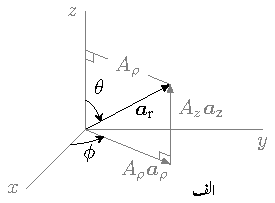
\includegraphics{figVectorSphericalUnitRadial}
\end{subfigure}%
%
\begin{subfigure}{0.5\textwidth}
\centering
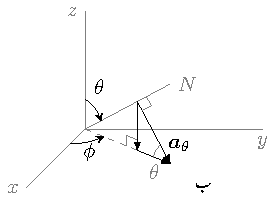
\includegraphics{figVectorSphericalUnitTheta}
\end{subfigure}%
\caption{کروی اکائی سمتیات کا کارتیسی نظام میں تبادلہ۔}
\label{شکل_سمتیہ_کروی_اکائی_رداسی_سمتیہ_کارتیسی}
\end{figure}

شکل \حوالہ{شکل_سمتیہ_کروی_تین_سطحوں_کا_ملاپ}-ب میں نقطہ \عددیء{N} پر اکائی سمتیات دکھائے گئے ہیں۔\عددیء{\ar} کی سمت تبدیل کئے بغیر اسے محدد کے مرکز پر منتقل کرتے ہوئے شکل \حوالہ{شکل_سمتیہ_کروی_اکائی_رداسی_سمتیہ_کارتیسی}-الف  میں دکھایا گیا ہے جہاں سے ظاہر ہے کہ اسے نلکی محدد کے اکائی سمتیات کی مدد سے
\begin{align}
\ar=A_\rho \arho+A_z \az
\end{align}
لکھا جا سکتا ہے۔شکل \حوالہ{شکل_سمتیہ_کروی_اکائی_رداسی_سمتیہ_کارتیسی}-الف  میں \عددیء{\ar} کی لمبائی ایک لیتے ہوئے  \عددیء{A_\rho=\sin \theta} اور \عددیء{A_z=\cos \theta} لکھا جا سکتا ہے۔یوں
\begin{align}\label{مساوات_سمتیہ_کروی_اکائی_نلکی_منتقل}
\ar=\sin \theta \arho+\cos \theta \az
\end{align}
حاصل ہوتا ہے۔اس مساوات کا باری باری \عددیء{\arho}، \عددیء{\aphi} اور \عددیء{\az} کے ساتھ غیر سمتی ضرب لیتے ہوئے
\begin{gather}
\begin{aligned}\label{مساوات_سمتیہ_کروی_رداس_نلکی_اکائی_غیر_سمتی_ضرب}
\ar \cdot \arho&=(\sin \theta \arho+\cos \theta \az) \cdot \arho=\sin \theta\\
\ar \cdot \aphi&=(\sin \theta \arho+\cos \theta \az) \cdot \aphi=0\\
\ar \cdot \az&=(\sin \theta \arho+\cos \theta \az) \cdot \az=\cos \theta
\end{aligned}
\end{gather}
حاصل ہوتا ہے جہاں \عددیء{\arho \cdot \arho=1}، \عددیء{\az \cdot \arho=0} وغیرہ کا استعمال کیا گیا۔یہ مساوات کروی رداسی اکائی سمتیے اور نلکی نظام کے اکائی سمتیات کے تمام ممکنہ غیر سمتی ضرب دیتا ہے۔اسی طرح جدول \حوالہ{جدول_سمتیہ_نلکی_کارتیسی_اکائی_غیر-سمتی_ضرب} استعمال کرتے ہوئے  مساوات  \حوالہ{مساوات_سمتیہ_کروی_اکائی_نلکی_منتقل} کا باری باری \عددیء{\ax} اور \عددیء{\ay} کے ساتھ غیر سمتی ضرب لیتے ہوئے
\begin{gather}
\begin{aligned}\label{مساوات_سمتیہ_کروی_رداس_کے_کارتیسی_اجزاء}
\ar \cdot \ax&=(\sin \theta \arho+\cos \theta \az) \cdot \ax=\sin \theta \cos \phi\\
\ar \cdot \ay&=(\sin \theta \arho+\cos \theta \az) \cdot \ay=\sin \theta \sin \phi\\
\ar \cdot \az&=(\sin \theta \arho+\cos \theta \az) \cdot \az=\cos \theta
\end{aligned}
\end{gather}
حاصل ہوتا ہے۔مکمل نتائج ایک جگہ لکھنے کی خاطر  مندرجہ بالا مساوات میں  \عددیء{\ar \cdot \az} کو بھی شامل کیا گیا ہے۔ یہ مساوات کروی اکائی رداسی  سمتیے  اور کارتیسی اکائی سمتیات کے تمام ممکنہ غیر سمتی ضرب دیتا ہے۔

\عددیء{\ar} کو کارتیسی نظام میں لکھنے کی خاطر \عددیء{\ar=\kvec{A}=A_x \ax+A_y \ay+A_z \az} لکھتے ہیں۔مساوات \حوالہ{مساوات_سمتیہ_کارتیسی_اجزاء} کے مطابق \عددیء{A_x=\ax \cdot \ar} جبکہ \عددیء{A_y=\ay \cdot \ar} اور \عددیء{A_z=\az \cdot \ar} ہوں گے۔یہ تمام  مساوات \حوالہ{مساوات_سمتیہ_کروی_رداس_کے_کارتیسی_اجزاء} میں دئے گئے ہیں۔ یوں 
\begin{align}
\ar=\sin \theta \cos \phi \ax+\sin \theta \sin \phi \ay+\cos \theta \az
\end{align}
لکھا جا سکتا ہے۔

شکل \حوالہ{شکل_سمتیہ_کروی_تین_سطحوں_کا_ملاپ}-ب میں دکھائے \عددیء{\atheta} کو \عددیء{\phi=\phi_0} سطح پر حرکت دیتے ہوئے  مرکز کے اتنے قریب لا کر شکل \حوالہ{شکل_سمتیہ_کروی_اکائی_رداسی_سمتیہ_کارتیسی}-ب میں دکھایا گیا ہے کہ اس کی نوک \عددیء{x=0} سطح کو چھوتی ہے۔جیسا شکل \حوالہ{شکل_سمتیہ_کروی_تین_سطحوں_کا_ملاپ}-الف سے واضح ہے،  \عددیء{\phi=\phi_0} سطح پر \عددیء{\atheta} کو حرکت دینے سے اس سمتیہ کی سمت تبدیل نہیں ہوتی۔شکل \حوالہ{شکل_سمتیہ_کروی_اکائی_رداسی_سمتیہ_کارتیسی}-ب کو دیکھتے ہوئے \عددیء{\atheta=B_\rho \arho-B_z \az} لکھا جا سکتا ہے۔یہاں رک کر  تسلی کر لیں کہ \عددیء{B_\rho \arho} اور \عددیء{\atheta} کے مابین زاویہ \عددیء{\theta} ہے۔\عددیء{\atheta}، \عددیء{B_\rho \arho} اور \عددیء{-B_z \az} مل کر تکون بناتے ہیں جسے دیکھتے ہوئے مسئلہ فیثاغورث کی مدد سے
\begin{align*}
B_\rho&=\cos \theta\\
B_z&=\sin \theta
\end{align*}
لکھا جا سکتا ہے۔یوں
\begin{align}\label{مساوات_سمتیہ_کروی_اکائی_تھیٹا}
\atheta=\cos \theta \arho-\sin \theta \az
\end{align}
کے برابر ہے۔اس مساوات کا باری باری \عددیء{\arho}، \عددیء{\aphi} اور \عددیء{\az} کے ساتھ غیر سمتی ضرب لینے سے
\begin{gather}
\begin{aligned}\label{مساوات_سمتیہ_کروی_تھیٹا_نلکی_اکائی_غیر_سمتی_ضرب}
\atheta \cdot \arho&=(\cos \theta \arho-\sin \theta \az) \cdot \arho=\cos \theta\\
\atheta \cdot \aphi&=(\cos \theta \arho-\sin \theta \az) \cdot \aphi=0\\
\atheta \cdot \az&=(\cos \theta \arho-\sin \theta \az) \cdot \az=-\sin \theta
\end{aligned}
\end{gather}
\عددیء{\atheta} اور نلکی اکائی سمتیات کے  تمام غیر سمتی ضرب حاصل ہوتے ہیں۔اسی طرح مساوات \حوالہ{مساوات_سمتیہ_کروی_اکائی_تھیٹا} کا باری باری \عددیء{ax}، \عددیء{\ay} اور \عددیء{\az} کے ساتھ غیر سمتی ضرب لینے سے
\begin{gather}
\begin{aligned}\label{مساوات_سمتیہ_کروی_تھیٹا_کے_کارتیسی_اجزاء}
\atheta \cdot \ax&=(\cos \theta \arho-\sin \theta \az) \cdot \ax=\cos \theta \arho \cdot \ax=\cos \theta \cos \phi\\
\atheta \cdot \ay&=(\cos \theta \arho-\sin \theta \az) \cdot \ay=\cos \theta \arho \cdot \ay=\cos \theta \sin \phi \\
\atheta \cdot \az&=(\cos \theta \arho-\sin \theta \az) \cdot \az=-\sin \theta \az \cdot \az=-\sin \theta
\end{aligned}
\end{gather}
حاصل ہوتے ہیں۔یہ مساوات \عددیء{\atheta} اور کارتیسی اکائی سمتیات کے تمام غیر سمتی ضرب دیتا ہے۔

\عددیء{\atheta} کو کارتیسی نظام میں لکھنے کی خاطر \عددیء{\atheta=\kvec{A}=A_x \ax+A_y\ay+A_z\az} لکھتے ہیں۔مساوات \حوالہ{مساوات_سمتیہ_کارتیسی_اجزاء} کے مطابق \عددیء{A_x=\ax \cdot \atheta} جبکہ \عددیء{A_y=\ay \cdot \atheta} اور \عددیء{A_z=\az \cdot \atheta} ہوں گے۔یہ تمام  مساوات \حوالہ{مساوات_سمتیہ_کروی_تھیٹا_کے_کارتیسی_اجزاء} میں دئے گئے ہیں۔ یوں
\begin{align}
\atheta=\cos \theta \cos \phi \ax+\cos \theta \sin \phi\ay-\sin \theta\az
\end{align}  
لکھا جا سکتا ہے۔

کروی  محدد کا \عددیء{\aphi} اور نلکی محدد کا \عددیء{\aphi} یکساں ہیں۔اسے کارتیسی نظام میں
\begin{align}
\aphi=-\sin \phi \ax+\cos \phi \ay
\end{align} 
لکھا جاتا ہے۔اس مساوات کا \عددیء{\ax}، \عددیء{\ay} اور \عددیء{\az} کے ساتھ غیر سمتی ضرب لیتے ہوئے
\begin{gather}
\begin{aligned}
\aphi \cdot \ax&=-\sin \phi\\
\aphi \cdot \ay&=\cos \phi\\
\aphi \cdot \az&=0
\end{aligned}
\end{gather}
لکھا جا سکتا ہے۔

مساوات \حوالہ{مساوات_سمتیہ_کروی_رداس_نلکی_اکائی_غیر_سمتی_ضرب} اور مساوات \حوالہ{مساوات_سمتیہ_کروی_تھیٹا_نلکی_اکائی_غیر_سمتی_ضرب} کے نتائج کے ساتھ \عددیء{\aphi} کے مختلف غیر سمتی ضربوں کو جدول \حوالہ{جدول_سمتیہ_کروی_نلکی_اکائی_غیر-سمتی_ضرب} میں یکجا کیا گیا ہے۔

\begin{table}
\caption{کروی  اکائی سمتیات کا نلکی اکائی سمتیات کے ساتھ غیر سمتی ضرب۔}
\centering
\begin{tabular}{l | r r r}
 & $\arho$ & $\aphi$ & $\az$ \\
\hline
$\ar$ & $\sin \theta$ & $0$& $\cos \theta$\\
$\atheta$ &$\cos \theta$ &$ 0$ &$ -\sin \theta$\\
$\aphi$ & $0$ &$ 1$ &$0$
\end{tabular}
\label{جدول_سمتیہ_کروی_نلکی_اکائی_غیر-سمتی_ضرب}
\end{table}
%

مساوات  \حوالہ{مساوات_سمتیہ_کروی_رداس_کے_کارتیسی_اجزاء} اور مساوات  \حوالہ{مساوات_سمتیہ_کروی_تھیٹا_کے_کارتیسی_اجزاء} کے نتائج جدول \حوالہ{جدول_سمتیہ_کروی_کارتیسی_اکائی_غیر-سمتی_ضرب} میں یکجا کئے گئے ہیں۔ 
\begin{table}
\caption{کروی  اکائی سمتیات کا کارتیسی اکائی سمتیات کے ساتھ غیر سمتی ضرب۔}
\centering
\begin{tabular}{l | r r r}
 & $\ax$ & $\ay$ & $\az$ \\
\hline
$\ar$ & $\sin \theta \cos \phi$ & $\sin \theta \sin \phi$& $\cos \theta$\\
$\atheta$ &$\cos \theta \cos \phi$ &$ \cos \theta \sin \phi$ &$ -\sin \theta$\\
$\aphi$ & $-\sin \phi$ &$ \cos \phi$ &$0$
\end{tabular}
\label{جدول_سمتیہ_کروی_کارتیسی_اکائی_غیر-سمتی_ضرب}
\end{table}
%
\begin{figure}
\centering
\begin{subfigure}{0.5\textwidth}
\centering
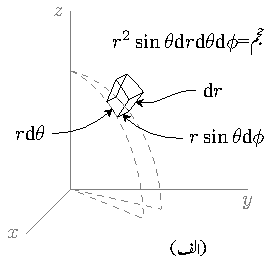
\includegraphics{figVectorSphericalDifferentialVolume}
\end{subfigure}%
%
\begin{subfigure}{0.5\textwidth}
\centering
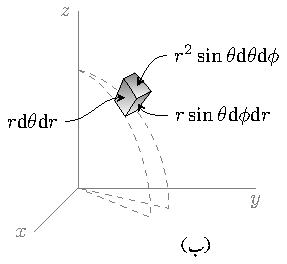
\includegraphics{figVectorSphericalDifferentialSurfaces}
\end{subfigure}%
\caption{(الف) کروی نظام میں  چھوٹی لمبائیاں اور چھوٹی حجم۔ (ب) کروی محدد میں چھوٹی سطحیں۔}
\label{شکل_سمتیہ_کروی_چھوٹی_حجم}
\end{figure}

شکل \حوالہ{شکل_سمتیہ_کروی_تین_سطحوں_کا_ملاپ} میں \عددیء{N(r,\theta,\phi)} پر تین عمودی سطحیں دکھائی گئی ہیں۔اگر کروی محدد کے متغیرات \عددیء{\dif r}، \عددیء{\dif \theta} اور \عددیء{\dif \phi} بڑھا کر دوبارہ تین عمودی سطحیں کھینچی جائیں تو یہ چھ سطحیں مل کر چھوٹا منحرف مکعب نما حجم گھیریں گی جسے شکل \حوالہ{شکل_سمتیہ_کروی_چھوٹی_حجم} میں دکھایا گیا ہے۔\عددیء{\ar} سمت میں مکعب کے چار اطراف کی لمبائیاں \عددیء{\dif r} ہے۔\عددیء{\atheta} سمت میں \عددیء{z} محدد کے قریبی دو اطراف کی لمبائیاں \عددیء{r \dif \theta} جبکہ دو دور اطراف کی لمبائیاں \عددیء{(r+\dif r)\dif \theta} ہے جسے دو اجزاء کی صورت میں یوں  \عددیء{r \dif \theta +\dif r \dif \theta} لکھا جا سکتا ہے۔دور اطراف کے لمبائی کا پہلا جزو ہوبہو قریبی اطراف کی لمبائی ہے جبکہ اس کا دوسرا جزو دور اور قریبی اطراف کے لمبائیوں میں فرق کو ظاہر کرتی ہے۔ان دو اجزاء کی نسبت \عددیء{\tfrac{\dif r \dif \theta}{r \dif \theta}=\tfrac{\dif r}{r}}  کے برابر ہے۔\عددیء{\dif r} کو کم سے کم\حاشیہد{کسی بھی متغیرہ مثلاً \عددیء{r} میں چھوٹی سی تبدیلی کو \عددیء{\Delta r} لکھا جاتا ہے جبکہ اس میں کم سے کم تبدیلی کو \عددیء{\dif r} لکھا جاتا ہے۔\عددیء{\dif r} کو تقریباً صفر سمجھا جا سکتا ہے یعنی \عددیء{\dif r \to 0} ہوتا ہے۔} کرتے ہوئے اس نسبت کو کم سے کم کیا جا سکتا  ہے۔ایسا ہی کرتے ہوئے ہم \عددیء{\dif r \dif \theta} کو رد کرتے ہوئے ان چاروں اطراف کی لمبائیاں \عددیء{r \dif \theta} ہی لیتے ہیں۔اسی طریقہ کار سے  \عددیء{\aphi} اطراف کی لمبائیاں  \عددیء{r \sin \theta \dif \phi} لکھی جا سکتی ہے۔منحرف مکعب نما کے اطراف میں معمولی فرق کو نظرانداز کرتے ہوئے اسے مکعب نما تصور کیا جا سکتا ہے جس کے \عددیء{r=r_0} سطحوں کا رقبہ \عددیء{r^2 \sin \theta \dif \theta \dif \phi} جبکہ \عددیء{\theta=\theta_0} سطحوں کا رقبہ \عددیء{r \sin \theta \dif r \dif \phi} اور \عددیء{\phi=\phi_0} سطحوں کا رقبہ   \عددیء{r \dif r \dif \theta} ہو گا۔اس مکعب کا حجم \عددیء{r^2 \sin \theta \dif r \dif \theta \dif \phi} ہو گا۔


شکل \حوالہ{شکل_سمتیہ_کروی_چھوٹی_حجم} میں کروی محدد کے تینوں متغیرات تبدیل کرتے ہوئے ہم چھوٹے مکعب کے  \عددیء{N(r,\theta,\phi)} کونے سے
 \عددیء{N'(r+\dif r,\theta+\dif \theta,\phi+\dif \phi)} کونے پہنچتے ہیں۔\عددیء{N} سے \عددیء{N'} تک سمتیہ کو
\begin{align}\label{مساوات_سمتیہ_کروی_چھوٹا_فاصلہ}
\dif \kvec{L}=\dif r \ar+r \dif \theta \atheta+r\sin \theta \dif \phi \aphi
\end{align}
لکھا جاتا ہے۔یہ مساوات کسی بھی دو قریبی نقطوں کے درمیان سمتی فاصلہ دیتا ہے۔

کسی بھی مکمل بند سطح کی  سمت، سطح کے عمودی باہر جانب لی جاتی ہے۔شکل \حوالہ{شکل_سمتیہ_کروی_چھوٹی_حجم} میں \عددیء{r=r_0} سطح  مرکز کا قریبی سطح ہے۔اس سطح کے دو آپس میں الٹ عمودی اطراف \عددیء{\mp \ar} ہیں جن میں \عددیء{-\ar} بند سطح کی بیرونی سمت کو ظاہر کرتا ہے لہٰذا یہی اس سطح کی درست سمت ہے۔اس کے برعکس \عددیء{r=r_0+\dif r} سطح مرکز سے دور تر ہے۔اس سطح کے بھی دو آپس میں الٹ عمودی سمتیں \عددیء{\mp \ar} ہیں جن میں \عددیء{\ar} سطح کی درست سمت ہے۔یوں  \عددیء{r=r_0} سطح کا سمتی رقبہ \عددیء{-r^2 \sin \theta \dif \theta \dif \phi \ar} جبکہ \عددیء{r=r_0+\dif r} سطح کا سمتی رقبہ \عددیء{\عددیء{r^2 \sin \theta \dif \theta \dif \phi \ar}} ہے۔اسی طرح \عددیء{\theta=\theta_0} سطح کا سمتی رقبہ \عددیء{-r \sin \theta \dif r \dif \phi\atheta} جبکہ \عددیء{\theta=\theta_0+\dif \theta} سطح کا سمتی رقبہ\عددی{r \sin \theta \dif r \dif \phi\atheta} ہو گا۔\عددیء{\phi=\phi_0} سطح کا \عددیء{-r \dif r \dif \theta \aphi} اور \عددیء{\phi=\phi_0+\dif \phi} سطح کا سمتی رقبہ \عددیء{r \dif r \dif \theta \aphi} ہو گا۔

%===================
\ابتدا{مشق}
شکل \حوالہ{شکل_سمتیہ_کروی_چھوٹی_حجم} میں \عددیء{} سمت میں مرکز کے قریبی اور دور اطراف کی لمبائیاں لکھیں۔

جوابات:\عددیء{r \sin \theta \dif \phi}، \عددیء{r \sin(\theta+\dif \theta) \dif \phi}، \عددیء{(r+\dif r) \sin \theta \dif \phi} اور \عددیء{(r+\dif r) \sin(\theta+\dif \theta) \dif \phi}
\انتہا{مشق}
%=======================
\ابتدا{مثال}\شناخت{مثال_سمتیہ_نلکی_کارتیسی_غیر_سمتی_اکائی_ضرب}
دو اکائی سمتیات \عددیء{\kvec{a}_1} اور \عددیء{\kvec{a}_2} کا غیر سمتی ضرب \عددیء{\kvec{a}_1 \cdot \kvec{a}_2=(1)(1) \cos \alpha_{12}} یعنی ان کے مابین زاویے \عددیء{\alpha_{12}} کے کوسائن کے برابر ہوتا ہے۔غیر سمتی ضرب کے اس تعریف کو استعمال کرتے ہوئے \عددیء{\ax \cdot \arho}، \عددیء{\ay \cdot \arho}، \عددیء{\ax \cdot \aphi} اور \عددیء{\ay \cdot \aphi} حاصل کریں۔
\begin{figure}
\centering
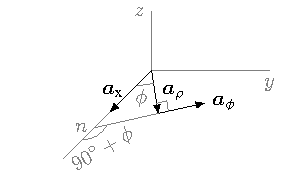
\includegraphics{figVectorDotProductUnitCartesianAndCylindrical}
\caption{کارتیسی اور نلکی اکائی سمتیات کا غیر سمتی ضرب۔}
\label{شکل_سمتیہ_غیر_سمتی_ضرب_بذریعہ_تعریف}
\end{figure}

حل:شکل \حوالہ{شکل_سمتیہ_غیر_سمتی_ضرب_بذریعہ_تعریف} میں \عددیء{\ax} اور \عددیء{\arho} کے درمیان زاویہ \عددیء{\phi} جبکہ \عددیء{\ay} اور \عددیء{\arho} کے درمیان زاویہ \عددیء{90^\circ-\phi} پایا جاتا ہے لہٰذا \عددیء{\ax \cdot \arho=\cos \phi} اور \عددیء{\ay \cdot \arho=\cos (90^\circ-\phi)=\sin \phi} کے برابر ہیں۔\عددیء{\ax} اور \عددیء{\aphi} کی سمتیں تبدیل کئے بغیر اگر انہیں یوں ہلایا جائے کہ ان کی دُم نقطہ \عددیء{n} پر آ ٹھرے تو شکل سے ظاہر ہے کہ ان کے مابین زاویہ \عددیء{90^\circ+\phi} ہے۔یوں \عددیء{\ax \cdot \aphi=\cos (90^\circ+\phi)=-\sin \phi} کے برابر ہے۔اسی طرح \عددیء{\ay} اور \عددیء{\aphi} کے درمیان \عددیء{\phi} زاویہ ہونے کی بنا پر \عددیء{\ay \cdot \aphi=\cos \phi} کے برابر ہے۔چونکہ \عددیء{\az} ان دونوں نلکی اکائی سمتیات کے عمودی ہے لہٰذا ان کا غیر سمتی ضرب صفر کے برابر ہو گا۔  
\انتہا{مثال}
%============
\begin{figure}
\centering
\begin{subfigure}{0.5\textwidth}
\centering
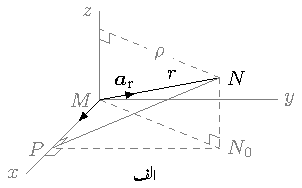
\includegraphics{figVectorSphericalUnitRadialDotWithCartesian}
\end{subfigure}%
%
\begin{subfigure}{0.5\textwidth}
\centering
\includegraphics{figVectorSphericalUnitThetaDotWithCartesian}
\end{subfigure}%
\caption{کروی اور کارتیسی اکائی سمتیات کا غیر سمتی ضرب۔}
\label{شکل_سمتیہ_کروی_کارتیسی_اکائی_غیر_سمتی_ضرب}
\end{figure}

\ابتدا{مثال}
مثال \حوالہ{مثال_سمتیہ_نلکی_کارتیسی_غیر_سمتی_اکائی_ضرب} کے طرز پر \عددیء{\ar}  کا \عددیء{\ax}، \عددیء{\ay} اور \عددیء{\az} کے ساتھ غیر سمتی ضرب حاصل کریں۔

حل: شکل \حوالہ{شکل_سمتیہ_کروی_کارتیسی_اکائی_غیر_سمتی_ضرب}-الف میں نقطہ \عددیء{N(r,\theta,\phi)} دکھایا گیا ہے جسے \عددیء{N(x,y,z)} بھی لکھا جا سکتا ہے۔شکل میں \عددیء{\ax} اور \عددیء{\ar} بھی دکھائے گئے ہیں۔شکل سے ظاہر ہے کہ \عددیء{\ax \cdot \ar=\cos \phase{NMP}} کے برابر ہے جہاں \عددیء{N} اور \عددیء{P} سے \عددیء{M} تک لکیریں کھینچنے سے زاویہ \عددیء{\phase{NMP}} بنتا ہے۔\عددیء{N} سے \عددیء{z=0} سطح پر عمود نقطہ \عددیء{N_0} دیتا ہے۔\عددیء{N_0} سے \عددیء{x} محدد پر عمود نقطہ \عددیء{P} دیتا ہے۔\عددیء{N} سے \عددیء{N_0} اور یہاں سے \عددیء{P} منتقل ہوتے ہوئے \عددیء{\ax} سمت میں کسی قسم کی حرکت نہیں کی جاتی لہٰذا اگر کارتیسی نظام میں \عددیء{N(x,y,z)} لکھا جائے تو اسی نظام میں \عددیء{N_0(x,y,0)} اور  \عددیء{P(x,0,0)} لکھے جائیں گے۔ہم \عددیء{N} سے \عددیء{x} محدد پر عمود بناتے ہوئے بھی \عددیء{P} تک پہنچ سکتے ہیں۔ تکون \عددیء{NMP} میں \عددیء{M} سے \عددیء{N} تک کا فاصلہ \عددیء{\overline{MN}=r} جبکہ \عددیء{M} سے \عددیء{P} تک کا فاصلہ \عددیء{\overline{MP}=x} اور زاویہ \عددیء{\phase{NPM}=90^\circ} ہیں لہٰذا \عددیء{\cos \phase{NMP}=\tfrac{x}{r}} ہو گا۔یہی  \عددیء{\ax} اور \عددیء{\ar} کے غیر سمتی ضرب  کے برابر ہے۔\عددیء{N} سے \عددیء{y} محدد پر عمود بناتے ہوئے یوں \عددیء{\ay \cdot \ar=\tfrac{y}{r}} اور \عددیء{N} سے \عددیء{z} محدد پر عمود سے \عددیء{\az \cdot \ar=\tfrac{z}{r}} لکھے جا سکتے ہیں۔چونکہ \عددیء{x=r\sin \theta \cos \phi}، \عددیء{y=r\sin \theta \sin \phi} اور \عددیء{z=r\cos \theta} کے برابر  ہیں لہٰذا ہم
\begin{align*}
\ar \cdot \ax&=\frac{x}{r}=\sin \theta \cos \phi\\
\ar \cdot \ay&=\frac{y}{r}=\sin \theta \sin \phi\\
\ar \cdot \az&=\frac{z}{r}=\cos \theta
\end{align*}
لکھ سکتے ہیں۔
\انتہا{مثال}
%=======================
\ابتدا{مثال}
مثال \حوالہ{مثال_سمتیہ_نلکی_کارتیسی_غیر_سمتی_اکائی_ضرب} کے طرز پر \عددیء{\atheta}  کا \عددیء{\ax} کے ساتھ غیر سمتی ضرب حاصل کریں۔

حل: شکل \حوالہ{شکل_سمتیہ_کروی_کارتیسی_اکائی_غیر_سمتی_ضرب}-ب میں نقطہ \عددیء{N} پر اکائی سمتیہ \عددیء{\atheta} جبکہ محدد کے مرکز \عددیء{M} پر \عددیء{\ax} دکھائے گئے ہیں۔\عددیء{\atheta \cdot \ax} حاصل کرنے کی خاطر سمتیات کی سمت تبدیل کئے بغیر انہیں \عددیء{z} محدد پر نقطہ \عددیء{B} منتقل کرتے ہوئے دوبارہ دکھایا گیا ہے جہاں سے واضح ہے کہ \عددیء{\atheta \cdot \ax=\cos \phase{ABC}} کے برابر ہے۔اس شکل میں \عددیء{\phase{DMC}=\phi} اور \عددیء{\phase{BMN}=\theta} کروی محدد کے زاویے ہیں۔تکون \عددیء{\Delta BMN} میں زاویہ \عددیء{\phase{MNB}} نوے درجے کا ہے۔یوں \عددیء{\phase{NBM}=90^\circ-\theta} ہو گا۔شکل سے واضح ہے کہ  \عددیء{\phase{NBM}=\phase{CBM}} ہیں۔اس طرح تکون \عددیء{\Delta BMC} میں \عددیء{\phase{BMC}=90^\circ} جبکہ \عددیء{\phase{CBM}=90^\circ-\theta} ہونے کی بنا پر \عددیء{\phase{MCB}=\theta} ہو گا۔

شکل-ب میں \عددیء{\overline{BM}=l} لیتے ہوئے تکون \عددیء{\Delta BMC}   کو دیکھتے ہوئے
\begin{align*}
\overline{BC}&=\frac{l}{\sin \theta}   \\
\overline{MC}&=\frac{l}{\tan \theta} 
\end{align*}
لکھا جا سکتا ہے۔تکون \عددیء{\Delta MDC} سے
\begin{align*}
\overline{MD}&=\overline{MC} \cos \phi=\frac{l \cos \phi}{\tan \theta} 
\end{align*} 
لکھا جا سکتا ہے۔شکل سے واضح ہے کہ \عددیء{\overline{MD}} اور \عددیء{\overline{AB}} برابر ہیں یعنی \عددیء{\overline{AB}=\overline{MD}}-یوں تکون \عددیء{\Delta BAC} سے
\begin{align*}
\cos \phase{ABC}&=\frac{\overline{AB}}{\overline{BC}}=\frac{\left(\frac{l \cos \phi}{\tan \theta}\right)}{\left(\frac{l}{\sin \theta}\right)}=\cos \theta \cos \phi
\end{align*}
حاصل ہوتا ہے۔یوں \عددیء{\ar \cdot \ax=\cos \theta \cos \phi} لکھا جا سکتا ہے۔
\انتہا{مثال}
%============

\ابتدا{مشق}
شکل \حوالہ{شکل_سمتیہ_کروی_کارتیسی_اکائی_غیر_سمتی_ضرب}-ب کے طرز پر شکل بناتے ہوئے \عددیء{\atheta \cdot \ay} اور \عددیء{\atheta \cdot \ay} حاصل کریں۔

جوابات:\عددیء{\cos \theta \sin \phi} اور \عددیء{-\sin \theta}
\انتہا{مشق}
%============

\newpage

\حصہء{سوالات}

\ابتدا{سوال}
سمتیہ \عددی{\kvec{A}=-2\ax+1\ay+7\az} اور \عددی{\kvec{B}=3\ax+5\ay-2\az} ہیں۔مندرجہ ذیل حاصل کریں: (الف) \عددی{2\kvec{A}-3\kvec{B}} اور اسی کی سمت میں اکائی سمتیہ؛ (ب) \عددی{2 \kvec{A}-5\kvec{B}+3\ax}؛ (پ) \عددی{\abs{3\kvec{A}}\abs{2\kvec{B}}(\kvec{B}-\kvec{A})}

جوابات: \عددی{-13\ax-13\ay+8\az}، \عددی{-0.648\ax-0.648\ay-0.399\az}، \عددی{28.3}، \عددی{1359\ax+1087\ay+1359\az}
\انتہا{سوال}

%=============================
\ابتدا{سوال}
نقطہ \عددی{A(1,-2,3)}، \عددی{B(3,-1,2)} اور \عددی{C(7,5,-4)} دیے گئے ہیں۔(الف) محدد کے مرکز سے \عددی{A} تک سمتیہ لکھیں؛ (ب) مرکز سے لکیر \عددی{AB} کے وسط تک سمتیہ لکھیں؛ (پ) اسی سمت میں اکائی سمتیہ لکھیں؛ (ت) تکون \عددی{ABC} کا احاطہ دریافت کریں۔

جوابات: \عددی{\ax-2\ay+3\az}، \عددی{2\ax-1.5\ay+2.5\az}، \عددی{0.566\ax-0.424\ay-0.707\az}، \عددی{23.4} 
\انتہا{سوال}
%==========================
\ابتدا{سوال}
مرکز سے نقطہ \عددیء{A} تک سمتیہ \عددیء{2\ax+\ay+3\az} ہے جبکہ مرکز سے \عددیء{\tfrac{2}{3}\ax-\tfrac{2}{3}\ay+\tfrac{1}{3}\az} اکائی سمتیہ کی سمت میں نقطہ \عددیء{B} پایا جاتا ہے۔دونوں نقطوں کے درمیان \عددیء{4} فاصلہ  ہونے کی صورت میں نقطہ \عددیء{B} دریافت کریں۔

جوابات:\عددیء{(2.57,-2.57,1.28)}
\انتہا{سوال}
%===============================
\ابتدا{سوال}
سمتی میدان \عددیء{\kvec{M}=(x+y^2)\ax+2(xy+3)\ay+4z^2\az} دیا گیا ہے۔نقطہ \عددیء{A(2,-3,1)} پر اس میدان کی قیمت حاصل کریں۔اسی نقطے پر میدان کی سمت میں اکائی سمتیہ دریافت کریں۔ایسی سطح جس پر \عددی{\abs{\kvec{M}}=5} ہو کی مساوات حاصل کریں۔اس سطح پر \عددیء{y=2} اور \عددیء{z=-1} ہونے کی صورت میں حاصل لکیر کی مساوات حاصل کریں۔

جوابات:\عددی{\kvec{M}=11\ax-6\ay+4\az}، \عددی{(0.836\ax-0.456\ay+0.304\az)}، \\ \عددی{x^2+y^2+2xy^2+4x^2y^2+24xy+16z^4-11=0}، \عددی{17x^2+56x+9=0}
\انتہا{سوال}
%===============================
\ابتدا{سوال}
سمتی میدان \عددی{\kvec{B}=2x^2\ax-3y(x+2z)\ay+5\az} اور \عددیء{\kvec{M}=(x+y+z)\ax+\tfrac{y}{x}\ay+xy\az} دیے گئے ہیں۔نقطہ \عددی{N(2,-3,-1)} پر \عددی{\kvec{B}} اور \عددیء{\kvec{M}} حاصل کریں۔اسی نقطے پر سمتیہ \عددیء{2\kvec{B}-\kvec{M}} کی سمت میں اکائی سمتیہ حاصل کریں۔

جوابات:\عددی{\kvec{B}=8\ax+5\az}، \عددی{\kvec{M}=-2\ax-1.5\ay-2\az}، \عددی{0.830\ax+0.069\ay+0.553\az}
\انتہا{سوال}
%================
\ابتدا{سوال}
 نقطہ \عددیء{N(2,-3,7))} پر میدان \عددیء{\kvec{M}=\tfrac{16}{x^2+y^2}(x\ax+y\ay)} کی سمت میں اکائی سمتیہ \عددی{\kvec{a}_M} دریافت کریں۔نقطہ \عددیء{N} پر \عددیء{\ax} اور \عددیء{\kvec{M}} کے درمیان زاویہ حاصل کریں۔اسی طرح نقطہ \عددیء{N} پر \عددیء{\ay} اور \عددیء{\kvec{M}} کے درمیان زاویہ حاصل کریں۔

جوابات:\عددی{\kvec{a}_M=0.555\ax-0.832\ay}، \عددی{56.3^{\circ}}، \عددی{33.7^{\circ}}
\انتہا{سوال}
%========================
\ابتدا{سوال}
میدان \عددیء{\kvec{M}=\tfrac{16}{x^2+y^2}(x\ax+y\ay)} کا مندرجہ ذیل دو درجی تکمل \عددی{y=3} سطح پر حاصل کریں۔
\begin{align*}
\int_{0}^{3} \int_{0}^{2} \kvec{M} \dif x \dif z\cdot \ax 
\end{align*}

جواب: \عددیء{24 \ln \frac{13}{9}}
\انتہا{سوال}
%========================
\ابتدا{سوال}
غیر سمتی ضرب استعمال کرتے ہوئے تکون \عددیء{ABC} میں زاویہ \عددی{A} اور \عددی{C} حاصل کریں۔تکون کے کونے \عددی{A(3,1,2)}، \عددی{B(4,6,2)} اور
 \عددی{C(1,4,-2)} ہیں۔

جوابات:\عددی{61.74^{\circ}} ، \عددیء{56.51^{\circ}}
\انتہا{سوال}
%===================
\ابتدا{سوال}
نقطے \عددیء{A(4,1,2)}، \عددیء{B(-2,4,3)} اور \عددیء{C(2,3,-1)} دیے گئے ہیں۔سمتیہ \عددی{\kvec{R}_{BA}} اور \عددی{\kvec{R}_{CA}} حاصل کریں۔دوسری سمتیہ  پر  پہلی سمتیہ کے \اصطلاح{عمودی سائے}\فرہنگ{عمودی سائے}\فرہنگ{سایہ!عمودی}\حاشیہب{projection}\فرہنگ{projection} کی لمبائی دریافت کریں۔لکیر \عددیء{AB} کے درمیانے نقطے سے لکیر \عددی{AC} کے درمیانے نقطے تک سیدھا سمتیہ حاصل کریں۔

جوابات: \عددی{-6\ax+3\ay+\az}، \عددی{-2\ax+2\ay-3\az}، \عددی{4.12}، \عددی{2\ax-0.5\ay-2\az}
\انتہا{سوال}
%==================
\ابتدا{سوال}
سمتیہ \عددیء{\kvec{M}=5\ax-3\ay+2\az} کا وہ حصہ حاصل کریں جو سمتیہ \عددی{\kvec{P}=-7\ax+2\ay-6\az} کے متوازی ہے۔وہ حصہ حاصل کریں جو اس کے عمودی ہے۔ 

جوابات: \عددی{4.17\ax-1.19\ay+3.57\az}، \عددی{0.83\ax-1.81\ay-1.57\az}
\انتہا{سوال}
%================
\ابتدا{سوال}
تین سمتیات \عددی{\kvec{r}_1=2\ax-1\ay+3\az}، \عددی{\kvec{r}_2=-3\ax+4\ay-5\az} اور \عددی{\kvec{r}_3=5\ax-2\ay+3\az} دیے گئے ہیں۔\عددیء{\kvec{r}_1\times \kvec{r}_2} کی سمت میں اکائی سمتیہ حاصل کریں۔ایسی اکائی سمتیہ حاصل کریں جو \عددیء{\kvec{r}_1} اور \عددیء{\kvec{r}_2} دونوں کو عمودی ہو۔سمتیہ \عددیء{\kvec{r}_2-\kvec{r}_1} اور \عددیء{\kvec{r}_2-\kvec{r}_3} دونوں کو عمودی اکائی سمتیہ حاصل کریں۔اس تکون کا رقبہ حاصل کریں جس کے اطراف \عددیء{\kvec{r}_1} اور \عددیء{\kvec{r}_2} ہوں۔اس تکون کا رقبہ حاصل کریں جس کے کونے یہ تین سمتیات دیتے ہیں۔ 

جوابات:\عددی{-0.81\ax+0.16\ay+0.58\az}، \عددی{\mp(-0.81\ax+0.16\ay+0.58\az)}، \\
\عددی{\mp(0.29\ax+0.88\ay+0.37\az)}، \عددی{4.3}، \عددی{13.6}
\انتہا{سوال}
%===============
\ابتدا{سوال}
نقطہ \عددی{N(5,10,4)} پر سمتیات \عددیء{\kvec{R}_{AN}=-3\ax+6\ay+12\az} اور \عددیء{\kvec{R}_{BN}=12\ax+20\ay-5\az} مل کر تکون بناتی ہیں۔تکون کی عمودی اکائی سمتیہ حاصل کریں۔سمتیہ \عددی{\kvec{R}_{BN}} کے عمودی اور تکون کی سطح کے متوازی اکائی سمتیہ حاصل کریں۔تکون کی سطح پر اس اکائی سمتیہ کو حاصل کریں جو نقطہ \عددیء{N} پر تکون کے کونے کو نصف زاویہ میں کاٹے۔

جوابات:\عددی{\mp(-0.83\ax+0.39\ay-0.40\az)}، \عددی{\mp(0.26\ax-0.38\ay-0.89\az)}، \\
\عددی{0.19\ax+0.87\ay+0.45\az}
\انتہا{سوال}
%=============
\ابتدا{سوال}
سمتیہ \عددی{\kvec{M}=(x^2+y^2)^{-1}(x\ax+y\ay)} کو نلکی محدد کے متغیرات میں لکھیں۔نقطہ \عددیء{(5,30^{\circ},6)} پر سمتیہ کی قیمت کارتیسی اور نلکی محدد میں حاصل کریں۔

جوابات:\عددی{\kvec{M}=\tfrac{1}{\rho}\arho}، \عددیء{\kvec{M}=0.41\ax+0.29\ay}، \عددی{\kvec{M}=\tfrac{1}{5}\arho}
\انتہا{سوال}
%===============
\ابتدا{سوال}
نقطہ \عددی{N(\rho=2,\phi=45^{\circ},z=12)} اور \عددیء{P(\rho=5,\phi=-60^{\circ},z=-6)} دئے گئے ہیں۔کارتیسی محدد میں، پہلے نقطے سے دوسرے نقطے کی جانب اکائی سمتیہ حاصل کریں۔اسی اکائی سمتیہ کو پہلے نقطے پر پائے جانے والے نلکی محدد کے متغیرات کی صورت میں لکھیں۔اسی اکائی سمتیہ کو دوسرے نقطے پر پائے جانے والے نلکی محدد کے متغیرات کی صورت میں لکھیں۔

جوابات: \عددی{0.057\ax-0.303\ay-0.951\az}، \عددی{-0.174\arho-0.255\aphi-0.951\az}، \عددی{0.292\arho-0.180\aphi-0.951\az}
\انتہا{سوال}
%================
\ابتدا{سوال}
نقطہ \عددیء{N(\rho=5,\phi=30^{\circ},z=6)} سے نقطہ \عددی{P(\rho=10,\phi=75^{\circ},z=12)} تک سمتیہ کارتیسی محدد میں لکھیں۔اسی سمت میں اکائی سمتیہ بھی لکھیں۔کارتیسی محدد میں دوسرے نقطے سے مرکز تک اکائی سمتیہ لکھیں۔

جوابات:\عددی{-1.74\ax+7.16\ay+6\az}، \عددیء{-0.183\ax-0.618\ay+0.631\az}، \\ \عددی{0.166\ax-0.618\ay-0.768\az}
\انتہا{سوال}
%================
\ابتدا{سوال}
نقطہ \عددی{M(5,-3,2)} سے نقطہ \عددیء{N(10,2,-5)} تک سمتیہ کو نقطہ \عددی{M} پر نلکی محدد کے اکائی سمتیات کی مدد سے لکھیں۔دوسرے نقطے سے پہلے نقطے کی سمت میں اکائی سمتیہ کو دوسرے  نقطے پر نلکی اکائی سمتیات کی مدد سے لکھیں۔دوسرے نقطے سے مرکز تک اکائی سمتیہ دوسرے نقطے کے اکائی سمتیات کی صورت  میں لکھیں۔ 

جوابات: \عددی{-1.71\arho-6.86\aphi+7\az}، \عددی{0.59\arho+0.39\aphi-0.7\az}، \عددی{0.90\arho+0.44\az} 
\انتہا{سوال}
%================
\ابتدا{سوال}
رداس \عددی{\rho=2} اور \عددیء{\rho=6} حجم گھیرتے ہیں جو \عددی{z=11} تا \عددیء{z=13} اور \عددی{\phi=30^{\circ}} تا \عددی{\phi=60^{\circ}} پایا جاتا ہے۔اس جسم کے حجم کو تین درجی تکمل سے حاصل کریں۔اس کی بھی تکمل سے سطح بھی حاصل کریں۔

جوابات: \عددی{16.8}، \عددی{41.1}
\انتہا{سوال}
%==================
\ابتدا{سوال}
نقطہ \عددیء{N(5,3,8)} سے نقطہ \عددی{P(3,-4,2)} تک سمتیہ کارتیسی، نلکی اور کروی محدد میں حاصل کریں۔پہلے نقطے کے اکائی سمتیات استعمال کریں۔تینوں سمتیات کی لمبائی حاصل کرتے ہوئے ثابت کریں کہ تینوں سمتیات کی لمبائی برابر ہے۔

جوابات:\عددی{-2\ax-7\ay-6\az}، \عددی{-5.3165\arho-4.9735\aphi-6.0000\az}، \\
 \عددی{  -8.6615\ar-2.7739\atheta-2.5069\aphi}، \عددی{9.434}
\انتہا{سوال}
%==================
\ابتدا{سوال}
نقطہ \عددی{N} پر سمتیہ \عددی{\kvec{K}=3\ar-2\atheta+8\aphi} اور \عددی{\kvec{G}=2\ar+5\atheta+2\aphi} دیے گئے ہیں۔ان کی غیر سمتی ضرب \عددی{\kvec{K}\cdot\kvec{G}} حاصل کریں۔دوسری سمتیہ کی پہلی سمتیہ کی سمت میں لمبائی حاصل کریں۔پہلی سمتیہ کا وہ حصہ دریافت کریں جو دوسری سمتیہ کی سمت میں ہے۔دونوں سمتیوں کا سمتی ضرب \عددی{\kvec{K} \times \kvec{G}} حاصل کریں۔اس نقطے پر دونوں سمتیوں کی عمودی اکائی سمتیہ حاصل کریں۔

جوابات:\عددی{12}، \عددی{1.3675}، \عددی{0.46753\ar-0.31169\atheta+1.24675\aphi}، \عددی{  44\ar-10\atheta-19\aphi}،\\ \عددی{\mp(  0.89871\ar-0.20425\atheta-0.38808\aphi)}
\انتہا{سوال}
%=====================
\ابتدا{سوال}
ایک جسم \عددی{r=6} تا \عددی{r=10}، \عددی{\theta=30^{\circ}} تا \عددی{\theta=70^{\circ}} اور \عددی{\phi=25^{\circ}} تا \عددی{\phi=100^{\circ}} حجم گھیرتا ہے۔اس جسم کے دو دور ترین کونوں کے درمیان فاصل حاصل کریں۔جسم کی سطح کا رقبے حاصل کریں۔جسم کی حجم دریافت کریں۔

جوابات:\عددی{9.27}، \عددی{198.27}، \عددی{179.25}
\انتہا{سوال}
%====================
\ابتدا{سوال}
نقطہ \عددی{N(5,4,-2)} اور \عددی{P(6,4,10)} دیے گئے ہیں۔پہلے نقطے کو نلکی محدد میں لکھیں۔پہلے نقطے کے متغیرات استعمال کرتے ہوئے پہلے نقطے سے دوسرے نقطے تک سمتیہ نلکی محدد میں لکھیں۔

جوابات:\عددی{P(6.4031,38.6598^{\circ},-2.0000)}، \عددی{  0.57\arho-0.82\aphi+12\az}
\انتہا{سوال}
%==================

\باب{کولمب کا قانون}\شناخت{باب_کولمب_قانون}
\حصہ{قوت کشش یا دفع}
نیوٹن کے \اصطلاح{کائناتی تجاذب کے قانون}\فرہنگ{تجاذب}\حاشیہب{Law of Universal Gravitation} سے آپ بخوبی واقف ہوں گے۔\اصطلاح{کولمب کا قانون}\فرہنگ{کولمب کا قانون}\حاشیہب{Coulomb's law} اس سے قریبی مشابہت رکھتا ہے۔کائناتی تجاذب کے قانون کو مساوات \حوالہ{مساوات_کولوم_کشش_ثقل} میں پیش کیا گیا ہے۔
\begin{align}\label{مساوات_کولوم_کشش_ثقل}
F&=G \frac{M_1 M_2}{R^2}
\end{align}
یہ مساوات کمیت \عددیء{M_1} اور کمیت \عددیء{M_2} کے مابین قوت کشش \عددیء{F} دیتی ہے جہاں ایک کمیت کے مرکز سے دوسری کمیت کے مرکز تک کا فاصلہ \عددیء{R} ہے۔قوت کشش دونوں کمیت کے حاصل ضرب کے  راست متناسب اور ان کے مرکزوں کے درمیان فاصلے  کے مربع کے بالعکس متناسب ہوتی ہے۔دونوں کمیتوں پر قوت کشش کی مقدار برابر ہوتی ہے اور یہ قوت دونوں کمیتوں کے  مرکزوں  کو ملانے والی لکیر پر پائی جاتی ہے۔\عددیء{M_1} پر قوت کشش کی سمت \عددیء{M_1} کے مرکز سے \عددیء{M_2} کے مرکز کی جانب  ہوتی ہے جبکہ \عددیء{M_2} پر قوت کشش کی سمت \عددیء{M_2} کے مرکز سے \عددیء{M_1} کے مرکز کی جانب ہوتی ہے۔تناسب کے جزو مستقل کو \عددیء{G} لکھا اور \اصطلاح{تجاذبی مستقل}\فرہنگ{تجاذبی مستقل}\حاشیہب{gravitational constant}\فرہنگ{gravitational constant} کہا جاتا ہے جس کی قیمت تقریباً \عددیء{\SI{6.674e-11}{\meter \cubed \per \kilo \gram \per \second \squared}} کے برابر ہے۔کرہ ارض کے ثقلی میدان میں  کمیت (میکانی بار) \عددی{m} کو اٹھانے کی خاطر \عددی{F=m g} قوت درکار ہوتی  ہے جہاں \عددی{g=\SI{9.8}{\meter\per\second\squared}} کے برابر ہے۔

کولمب کا قانون مساوات \حوالہ{مساوات_کولوم_کولمب_کشش_بار} میں بیان کیا گیا ہے۔یہ مساوات \اصطلاح{برقی بار}\فرہنگ{برقی بار}\حاشیہب{charge}\فرہنگ{charge} \عددیء{Q_1} اور برقی بار \عددیء{Q_2} کے مابین قوت کشش یا قوت دفع \عددیء{F} دیتی ہے جہاں ایک برقی بار کے مرکز سے دوسری برقی بار کے مرکز تک کا فاصلہ \عددیء{R} ہے۔ان برقی باروں کا حجم صفر تصور کیا جاتا ہے۔یوں اگر برقی بار کو گیند کی شکل کا تصور کیا جائے تو اس گیند کے رداس  کی لمبائی صفر ہو گی۔ایسے برقی بار کو \اصطلاح{نقطہ برقی بار}\فرہنگ{نقطہ برقی بار}\حاشیہب{point charge}\فرہنگ{point charge} کہا جاتا ہے۔برقی بار کی اصطلاح کو چھوٹا کرتے ہوئے اسے \اصطلاح{بار}\فرہنگ{بار} کہا جائے گا۔
\begin{align}\label{مساوات_کولوم_کولمب_کشش_بار}
F&=\frac{1}{4 \pi \epsilon_0}\frac{Q_1 Q_2}{ R^2}
\end{align}

قوت کشش یا دفع دونوں برقی باروں کے حاصل ضرب کے  راست متناسب  اور باہمی فاصلہ کے  مربع کے بالعکس متناسب ہوتی ہے۔دونوں برقی باروں پر قوت کی مقدار برابر ہوتی ہے اور یہ قوت دونوں برقی باروں سے گزرتی لکیر پر عمل درآمد ہوتی ہے۔دو مختلف اقسام کے برقی باروں کے مابین قوت کشش پائی جاتی ہے جبکہ دو یکساں برقی باروں کے مابین قوت دفع پائی جاتی ہے۔مساوات کے جزو مستقل کو \عددیء{\tfrac{1}{4 \pi \epsilon_0}} لکھا جاتا ہے جہاں \عددیء{\epsilon_0} خلاء  کا \اصطلاح{برقی مستقل}\فرہنگ{برقی مستقل}\حاشیہب{permittivity}\فرہنگ{permittivity}\حاشیہب{electric constant}\فرہنگ{electric constant} ہے جس کی قیمت اٹل ہے۔خلاء کے برقی مستقل کی قیمت
\begin{align}
\epsilon_0=\frac{1}{\mu_0 c^2}
\end{align}
ہے جہاں \عددیء{c} خلاء میں روشنی کی رفتار اور \عددیء{\mu_0} خلاء کی \اصطلاح{مقناطیسی مستقل}\فرہنگ{مقناطیسی مستقل}\حاشیہب{permeability constant}\فرہنگ{permeability constant} ہے۔یہ دونوں بھی اٹل مستقل ہیں جن کی قیمتیں
\begin{align}
c&=\SI{299792458}{\meter \per \second} \approx \SI{3e8}{\meter \per \second}\\
\mu_0&=\SI{4 \numpi e-7}{\henry \per \meter}
\end{align}
 ہیں۔یوں مقناطیسی مستقل  کی قیمت تقریباً
\begin{align}
\epsilon_0 =\num{8.854e-12} \overset{.}{=}\frac{1}{36 \pi} 10^{-9} \si{\farad \per \meter}
\end{align}
 کے برابر ہے۔اس کتاب میں \عددیء{\tfrac{1}{4 \pi \epsilon_0}} بار بار استعمال ہو گا جسے عموماً
\begin{align}\label{مساوات_کولمب_برقی_مستقل_قیمت_الف}
\frac{1}{4 \pi \epsilon_0} \overset{.}{=} 9 \times 10^9
\end{align}
لیا جائے گا۔\عددیء{\epsilon_0}  کی اکائی فیراڈ فی میٹر  \عددیء{\si{\farad \per \meter}} ہے  جس کی وضاحت جلد کر دی جائے گی۔

\ابتدا{مثال}
سطح زمین پر زمین اور ایک کلو گرام کمیت کے مابین \عددیء{\SI{9.8}{\newton}} کی قوت کشش پائی جاتی ہے۔زمین کا رداس \عددیء{\SI{6370}{\kilo \meter}} لیتے ہوئے زمین کی کمیت حاصل کریں۔

حل:مساوات \حوالہ{مساوات_کولوم_کشش_ثقل} کی مدد سے
\begin{align*}
9.8=\frac{6.674 \times 10^{-11} \times M \times 1}{\num{6370000} \times \num{6370000}}\\
\end{align*}
لکھتے ہوئے زمین کی کمیت \عددیء{\SI{5.959e24}{\kilo \gram}} حاصل ہوتی ہے۔
\انتہا{مثال}
%===========================
\ابتدا{مثال}
زمین کے مرکز سے تقریباً \عددیء{\SI{42000}{\kilo \meter}} کے فاصلے پر ذرائع ابلاغ کے سیٹلّائٹ زمین کے گرد مدار میں گردش کرتے ہیں۔پوری دنیا میں \اصطلاح{بے تار}\فرہنگ{بے تار}\حاشیہب{wireless}\فرہنگ{wireless} مواصلاتی نظام اسی کا مرہون منت ہے۔اس فاصلے پر ایک کلو گرام کی کمیت اور زمین کے مابین قوت کشش کی مقدار حاصل کریں۔

حل: 
\begin{align*}
F=\frac{6.674 \times 10^{-11} \times 5.959 \times 10^{24} \times 1}{\num{42000000} \times \num{42000000}}=\SI{0.225}{\newton}\\
\end{align*}
\انتہا{مثال}
%============================
\ابتدا{مثال}
ایک ایک کولمب کے دو مثبت برقی باروں کے درمیان  ایک میٹر کا فاصلہ ہے۔ان میں قوت دفع حاصل کریں۔

حل: \عددیء{\tfrac{1}{4\pi \epsilon_0}} کی قیمت مساوات \حوالہ{مساوات_کولمب_برقی_مستقل_قیمت_الف} سے لیتے ہوئے
\begin{align*}
F&=9 \times 10^9 \frac{1 \times 1}{1 \times 1}=\SI{9e9}{\newton}
\end{align*}
\انتہا{مثال}
%===================

مندرجہ بالا مثال سے  آپ دیکھ سکتے ہیں کہ برقی بار کی اکائی (کولمب)  انتہائی بڑی مقدار ہے۔

شکل \حوالہ{شکل_سمتیہ_دو_مثبت_بار_قوت_دفع} میں بار \عددیء{Q_1} محدد کے مرکز سے سمتی فاصلہ \سمتیہ{r_1} پر جبکہ بار \عددیء{Q_2} مرکز سے سمتی فاصلہ \سمتیہ{r_2} پر دکھایا گیا ہے۔بار \عددیء{Q_1} سے بار \عددیء{Q_2} تک کا سمتی فاصلہ \سمتیہ{R_{21}} ہے جہاں
\begin{align}
\kvec{R_{21}}=\kvec{r_2}-\kvec{r_1}
\end{align}
کے برابر ہے۔سمتیہ \سمتیہ{R_{21}} کی سمت میں اکائی سمتیہ \سمتیہ{a_{21}} یوں حاصل کیا جاتا ہے
\begin{align}
\kvec{a_{21}}=\frac{\kvec{R_{21}}}{\abs{\kvec{R_{21}}}}=\frac{\kvec{R_{21}}}{R_{21}}=\frac{\kvec{r_2}-\kvec{r_1}}{\abs{\kvec{r_2}-\kvec{r_1}}}
\end{align}
بار \عددیء{Q_2} پر قوت \سمتیہ{F_2} کی حتمی قیمت مساوات  \حوالہ{مساوات_کولوم_کولمب_کشش_بار} سے حاصل کی جا سکتی ہے جبکہ اس کی سمت اکائی سمتیہ \سمتیہ{a_{21}} کے سمت میں ہو گی۔اس طرح یہ قوت
\begin{gather}
\begin{aligned}\label{مساوات_کولمب_قوت_کی_مساوات_الف}
\kvec{F_2}&=\frac{1}{4 \pi \epsilon_0}\frac{Q_1 Q_2}{ R_{21}^2} {\kvec{a_{21}}}\\
&=\frac{Q_1 Q_2}{4 \pi \epsilon_0}\frac{\kvec{r_2}-\kvec{r_1}}{\abs{\kvec{r_2}-\kvec{r_1}}^3}
\end{aligned}
\end{gather}
لکھی جائے گی۔مساوات \حوالہ{مساوات_کولمب_قوت_کی_مساوات_الف} کولمب کے قانون کی سمتی شکل ہے۔چونکہ دونوں باروں پر برابر مگر الٹ سمت میں قوت عمل کرتی ہے لہٰذا \عددیء{Q_1} پر قوت \سمتیہ{F_1} یوں لکھا جائے گا
 \begin{gather}
\begin{aligned}
\kvec{F_1}=-\kvec{F_2}&=\frac{-1}{4 \pi \epsilon_0}\frac{Q_1 Q_2}{ R_{21}^2} \kvec{a_{21}}\\
&=\frac{1}{4 \pi \epsilon_0}\frac{Q_1 Q_2}{ R^2} {\kvec{a_{12}}}
\end{aligned}
\end{gather}
جہاں دوسری قدم پر \عددیء{R_{21}=R_{12}=R} لکھا گیا ہے اور \عددیء{\kvec{a_{12}}=-\kvec{a_{21}}} کے برابر ہے۔
%
\begin{figure}
\centering
\includegraphics{figCoulombForceBetweenTwoCharges}
\caption{دو مثبت باروں کے مابین قوت دفع}
\label{شکل_سمتیہ_دو_مثبت_بار_قوت_دفع}
\end{figure}
دونوں بار مثبت یا دونوں بار منفی ہونے کی صورت میں \عددیء{Q_2} پر مساوات \حوالہ{مساوات_کولمب_قوت_کی_مساوات_الف} سے قوت \سمتیہ{a_{21}} کی سمت میں حاصل ہوتی ہے۔یوں یکساں باروں کے مابین قوت دفع پائی جاتی ہے۔دو الٹ اقسام کے باروں کی صورت میں \عددیء{Q_2} پر قوت \سمتیہ{-a_{21}} کی سمت میں حاصل ہوتا ہے۔یوں الٹ اقسام کے باروں کے مابین قوت کشش پائی جاتی ہے۔  

\ابتدا{مثال}
شکل \حوالہ{شکل_سمتیہ_دو_مثبت_بار_قوت_دفع} میں نقطہ \عددیء{A(3,2,4)} پر \عددیء{\SI{20}{\micro \coulomb}} کا بار \عددیء{Q_1} جبکہ نقطہ \عددیء{B(1,5,9)} پر \عددیء{\SI{-50}{\micro \coulomb}} کا بار \عددیء{Q_2} پایا جاتا ہے۔منفی بار \عددیء{Q_2} پر سمتی قوت حاصل کریں۔

حل:
\begin{align*}
\kvec{R_{21}}&=(1-3) \ax+(5-2) \ay+(9-4)\az\\
&=-2 \ax+3 \ay+5 \az\\
R_{21}&=\abs{\kvec{R_{21}}}=\sqrt{(-2)^2+3^2+5^2}\\
&=\sqrt{38}\\
&=6.1644
\end{align*}
اور یوں
\begin{align*}
\kvec{a_{21}}&=\frac{{\kvec{R_{21}}}}{\abs{\kvec{R}_{21}}}=\frac{-2 {\ax}+3 {\ay}+5 \az}{6.1644}\\
&=-0.324 \ax+0.487 \ay+0.811\az
\end{align*}
حاصل ہوتا ہے جس سے
\begin{align*}
\kvec{F_2}&=\frac{36 \pi  \times 10^9}{4 \pi} \frac{\left (-50\times 10^{-6} \times 20 \times 10^{-6} \right )}{38} \left(-0.324 \ax+0.487 \ay+0.811\az\right)\\
&=-0.237  \left(-0.324 \ax+0.487 \ay+0.811\az \right) \, \si{\newton}
\end{align*}
حاصل ہوتا ہے۔آپ دیکھ سکتے ہیں کہ قوت کی سمت \سمتیہ{a_{21}} کے الٹ سمت میں ہے۔یوں منفی بار پر قوت کی سمت مثبت بار کی جانب ہے یعنی اس پر قوت کشش پائی جاتی ہے۔
\انتہا{مثال}
%========================
کسی بھی بار پر ایک سے زیادہ باروں سے پیدا مجموعی قوت تمام باروں سے پیدا علیحدہ علیحدہ قوتوں کا سمتی مجموعہ ہوتا ہے یعنی
\begin{align}
\kvec{F}=\sum_{i=1}^n \kvec{F}_i
\end{align}
اس حقیقت کو یوں بیان کیا جاتا ہے کہ کولمب کا قانون \اصطلاح{خطی}\فرہنگ{خطی}\حاشیہب{linear}\فرہنگ{linear} ہے۔ 

%========================
\حصہ{برقی میدان کی شدت}
نیوٹن کے کائناتی تجاذب کے قانون میں زمین کی کمیت کو \عددیء{M} لکھ کر کمیت \عددیء{m} پر قوت \عددیء{F} حاصل کی جا سکتی ہے۔ایک کلوگرام کمیت پر اس قوت کی مقدار \عددیء{\tfrac{F}{m}} ہو گی جسے \اصطلاح{زمین کی کشش}\فرہنگ{کشش!زمین}\حاشیہب{gravity}\فرہنگ{gravity} یا \اصطلاح{ثقلی اسراع} کہا اور \عددیء{g} لکھا جاتا ہے۔زمین کی سطح پر \عددیء{g} کی مقدار تقریباً \عددیء{\SI{9.8}{\meter \per \second \squared}} کے برابر ہے۔
\begin{align}\label{مساوات_کولمب_زمین_کی_کشش}
g&=\frac{F}{m}=\frac{GM}{R^2}
\end{align}

کسی بھی کمیت \عددیء{M} کے گرد  \اصطلاح{تجاذبی میدان}\حاشیہب{gravitational field}\فرہنگ{تجاذبی میدان} پایا جاتا ہے۔ کسی بھی نقطے پر  اس تجاذبی میدان کو ناپنے کی خاطر اس نقطے پر پیمائشی کمیت \عددیء{m_p}\حاشیہد{\عددیء{m_p} لکھتے ہوئے  زیرنوشت میں \عددیء{p} لفظ پیمائشی  کے \موٹا{پ} کو ظاہر کرتا ہے، یعنی یہ وہ کمیت ہے جسے قوت  کی پیمائش کی خاطر استعمال کیا جا رہا ہے۔} رکھ کر اس پر قوت ناپی جاتی ہے۔مختلف مقامات پر اس طرح قوت ناپ کر ہم تجاذبی میدان کا جائزہ لے سکتے ہیں۔تجاذبی قوت کی مقدار کا دارومدار پیمائشی کمیت \حاشیہب{test mass} \عددیء{m_p} پر بھی منحصر ہے۔مختلف تجاذبی میدانوں کا آپس میں موازنہ کرتے وقت یہ ضروری ہے کہ تمام تجاذبی میدان جانچتے وقت ایک ہی قیمت کے پیمائشی کمیت استعمال کی جائے۔ماہرین طبیعیات عموماً \عددیء{m_p} کو ایک کلوگرام  رکھتے ہیں۔یہ ضروری نہیں کہ تجاذبی قوت ناپتے وقت ایک کلوگرام کی پیمائشی کمیت ہی استعمال کی جائے البتہ جوابات اکٹھے کرتے وقت \سمتیہ{F} کو \عددیء{m_p} سے تقسیم کرتے ہوئے ایک کلوگرام پر تجاذبی قوت حاصل کی جا سکتی ہے۔زمین کے قریب ایک کلو گرام کمیت پر قوت کشش کو ثقلی اسراع \عددی{g} کہا جاتا ہے۔

\ابتدا{مثال}
زمین کی سطح پر دو سو گرام پیمائشی کمیت پر \عددیء{\SI{1.96}{\newton}} قوت ناپی جاتی ہے۔ثقلی اسراع حاصل کریں۔

حل:
\begin{align}
g=\frac{1.96}{0.2}=\SI{9.8}{\newton \per \kilogram}
\end{align}   
\انتہا{مثال}

مساوات \حوالہ{مساوات_کولمب_زمین_کی_کشش} سے ہم
\begin{gather}
\begin{aligned}
F&=m g\\
w&=m g
\end{aligned}
\end{gather}
لکھ سکتے ہیں جو زمین کی  سطح پر کمیت \عددیء{m} پر کشش ثقل \عددیء{F} دیتا ہے جسے  وزن پکارا اور  \عددیء{w} لکھا جاتا ہے۔
  
باروں پر بھی اسی طرح غور کیا جاتا ہے۔کسی بھی بار \عددیء{Q} کے گرد برقی میدان پایا جاتا ہے یعنی برقی میدان کا منبع بار ہے۔اس برقی میدان میں بار پر قوت اثر انداز ہوتی ہے۔بار \عددیء{Q} کے برقی میدان کی شدت کی پیمائش کی خاطر اس میدان میں مختلف مقامات پر پیمائشی بار \حاشیہب{test charge} \عددیء{q_p} پر قوت \سمتیہ{F} ناپ کر برقی میدان کا مطالعہ کیا جا سکتا ہے اور اس کا نقشہ بنایا جا سکتا ہے۔مختلف باروں کے برقی میدانوں کا آپس میں موازنہ کرتے وقت یہ ضروری ہے کہ تمام صورتوں میں ایک ہی قیمت کے پیمائشی بار  استعمال کئے جائیں۔ماہرین طبیعیات \عددیء{q_p} کو ایک کولمب کا مثبت بار  رکھتے ہیں۔یہ ضروری نہیں کہ قوت ناپتے وقت ایک کولمب کا مثبت پیمائشی بار ہی استعمال کیا جائے البتہ جوابات اکٹھے کرتے وقت \سمتیہ{F} کو \عددیء{q_p} سے تقسیم کرتے ہوئے ایک مثبت کولمب کے بار پر قوت حاصل کی جاتی ہے جسے \اصطلاح{برقی میدان کی شدت}\فرہنگ{برقی میدان!شدت}\فرہنگ{شدت!برقی}\حاشیہب{electric field intensity}\فرہنگ{electric field intensity} یا صرف \اصطلاح{برقی میدان} پکارا اور \سمتیہ{E} لکھا جاتا ہے یعنی
\begin{align}\label{مساوات_کولمب_برقی_شدت_اور_قوت}
\kvec{E}=\frac{\kvec{F}}{q_p}
\end{align}
مختلف مقامات پر موجود مختلف قیمتوں کے باروں سے کسی ایک نقطے پر  پیدا برقی میدان  تمام باروں کے مجموعی اثر سے پیدا ہو گا۔ایسا کولمب کے قانون کے خطی ہونے کی بنا پر ہوتا ہے۔کسی بھی نقطے پر \عددیء{n} باروں کا مجموعی \سمتیہ{E} تمام باروں کے علیحدہ علیحدہ پیدا کردہ  \سمتیازیرنوشت{E}{1}،  \سمتیازیرنوشت{E}{2}،\سمتیازیرنوشت{E}{3}،\عددیء{\cdots}  کا سمتی مجموعہ
\begin{align}
\kvec{E}=\sum_{i=1}^n \kvec{E}_i=\kvecsub{E}{1}+\kvecsub{E}{2}+\kvecsub{E}{3}+\cdots+\kvec{E}_n 
\end{align}
 ہوتا ہے۔یوں کسی بھی نقطے \عددیء{P}  پر \سمتیہ{E} ناپتے وقت اس نقطے پر ایک کولمب بار \عددیء{q_p} رکھ کر اس بار پر قوت ناپی جاتی ہے۔یہ قوت اس نقطے پر تمام باروں کا مجموعی  \سمتیہ{E} ہوتا ہے۔یاد رہے کہ کسی بھی نقطے پر  \سمتیہ{E} ناپتے وقت یہاں رکھے پیمائشی بار \عددیء{q_p} کا اثر شامل نہیں ہوتا۔

مساوات  \حوالہ{مساوات_کولمب_قوت_کی_مساوات_الف} سے  بار \عددیء{Q} سے \عددیء{\kvec{a}_R} سمت میں \عددیء{R} فاصلے پر برقی میدان کو
\begin{gather}
\begin{aligned}\label{مساوات_کولمب_قوت_کی_عمومی_مساوات}
\kvec{E}&=\frac{Q}{4 \pi \epsilon_0}\frac{\kvec{a_{R}}}{ R^2}\\
&=\frac{Q}{4 \pi \epsilon_0}\frac{\kvec{R}}{ R^3}
\end{aligned}
\end{gather}
لکھا جا سکتا ہے۔بار کو کروی محدد کے مرکز پر تصور کرتے ہوئے اسی مساوات کو یوں لکھا جا سکتا ہے
\begin{align}\label{مساوات_کولمب_نقطہ_بار_کروی_رداس_پر_تبدیل_نہیں_ہوتا}
\kvec{E}=\frac{Q}{4 \pi \epsilon_0 r^2} \ar
\end{align}
جہاں  \عددیء{\ar}  کروی محدد کا رداسی سمت میں اکائی سمتیہ ہے۔

نقطہ \عددیء{(x',y',z')} پر موجود بار \عددیء{Q} سے نقطہ \عددیء{(x,y,z)} پر برقی شدت  یوں حاصل کی جا سکتی ہے۔
\begin{gather}
\begin{aligned} \label{مساوات_کولمب_نقطہ_بار_سے_میدان_کا_حصول}
\kvec{E}&=\frac{1}{4 \pi \epsilon_0 }\frac{Q}{\abs{\kvec{r}-\kvec{r'}}^2} \frac{\kvec{r}-\kvec{r'}}{\abs{\kvec{r}-\kvec{r'}}}=\frac{Q}{4 \pi \epsilon_0 }\frac{\kvec{r}-\kvec{r'}}{\abs{\kvec{r}-\kvec{r'}}^3}\\
&=\frac{Q}{4 \pi \epsilon_0}\frac{\left[(x-x')\ax+(y-y')\ay+(z-z')\az\right]}{\left [(x-x')^2+(y-y')^2+(z-z')^2\right]^{\frac{3}{2}}}
\end{aligned}
\end{gather} 
جہاں
\begin{align*}
\kvec{r}&=x \ax+y \ay+z\az\\
\kvec{r'}&=x' \ax+y' \ay+z'\az\\
\kvec{R}&=\kvec{r}-\kvec{r'}=(x-x') \ax+(y-y') \ay+(z-z')\az
\end{align*}
کے برابر ہے۔
%===================
\ابتدا{مثال}
نقطہ \عددیء{N_1(4,1,1)} پر \عددیء{\SI{100}{\micro \coulomb}} کا بار \عددیء{Q_1} جبکہ نقطہ \عددیء{N_2(1,4,2)} پر \عددیء{\SI{50}{\micro \coulomb}} کا بار \عددیء{Q_2} پایا جاتا ہے۔نقطہ \عددیء{N_3(2,2,5)} پر  \عددیء{Q_1} سے پیدا \سمتیازیرنوشت{E}{1}  اور \عددیء{Q_2} سے پیدا \سمتیازیرنوشت{E}{2} حاصل کریں۔اس نقطے پر دونوں باروں کا مجموعی \عددیء{\kvec{E}} کیا ہو گا۔
\begin{figure}
\centering
\includegraphics[height=3.5cm]{figCoulombElectricFieldOfTwoCharges}
\caption{دو باروں سے پیدا برقی شدت}
\label{شکل_کولمب_دو_باروں_سے_پیدا_برقی_شدت}
\end{figure}

حل:شکل \حوالہ{شکل_کولمب_دو_باروں_سے_پیدا_برقی_شدت} میں صورت حال دکھایا گیا ہے۔پہلے \عددیء{Q_1} سے پیدا \سمتیازیرنوشت{E}{1} حاصل کرتے ہیں۔\عددیء{N_1}  سے \عددیء{N_3} تک سمتی فاصلہ
\begin{align*}
\kvecsub{R}{31}=\kvecsub{R}{3}-\kvecsub{R}{1}&=(2-4)\ax+(2-1)\ay+(5-1)\az\\
&=-2\ax+1\ay+4\az
\end{align*}
ہے جس سے
\begin{align*}
R_{31}&=\abs{\kvecsub{R}{31}}=\sqrt{(-2)^2+1^2+4^2}\\
&=\sqrt{21}=4.583\\
\kvecsub{a}{31}&=\frac{\kvecsub{R}{31}}{R_{31}}=\frac{-2\ax+1\ay+4\az}{\sqrt{21}}\\
&=-0.436\ax+0.218\ay+0.873\az
\end{align*}
حاصل ہوتے ہیں۔یوں مساوات \حوالہ{مساوات_کولمب_قوت_کی_عمومی_مساوات} سے
\begin{align*}
\kvecsub{E}{1}&=9 \times 10^9 \frac{100 \times 10^{-6}}{21} \left(-0.436\ax+0.218\ay+0.873\az\right)\\
&=-\num{18686}\ax+\num{9343}\ay+\num{37414}\az \quad \si{\volt \per \meter}
\end{align*}
حاصل ہوتا ہے جہاں مساوات \حوالہ{مساوات_کولمب_برقی_مستقل_قیمت_الف} سے \عددیء{\tfrac{1}{4\pi \epsilon_0}} کی قیمت \عددیء{9 \times 10^9} پر کی گئی۔اسی طرح \عددیء{Q_2} کے لئے حل کرتے ہوئے
\begin{align*}
\kvecsub{R}{32}&=(2-1)\ax+(2-4)\ay+(5-2)\az\\
&=1\ax-2\ay+3\az
\end{align*}
اور
\begin{align*}
R_{32}&=\abs{\kvecsub{R}{32}}=\sqrt{1^2+2^2+3^2}=\sqrt{14}\\
\kvecsub{a}{32}&=\frac{1\ax-2\ay+3\az}{\sqrt{14}}\\
&=0.267\ax-0.535\ay+0.802\az
\end{align*}
سے
\begin{align*}
\kvecsub{E}{2}&=9 \times 10^9 \frac{50 \times 10^{-6}}{14} \left(0.267\ax-0.535\ay+0.802\az \right)\\
&=\num{8582}\ax-\num{17196}\ay+\num{25779}\az \quad \si{\volt \per \meter}
\end{align*}
ملتا ہے۔ان دو جوابات کا سمتی مجموعہ لیتے ہوئے کُل \kvec{E} حاصل کرتے ہیں۔
\begin{align*}
\kvec{E}&=\kvecsub{E}{1}+\kvecsub{E}{2}\\
&=\left(\num{-18686} \ax+\num{9343} \ay+\num{37414}\az\right)+\left(\num{8582}\ax-\num{17196}\ay+\num{25779}\az\right)\\
&=-\num{10104}\ax-\num{7853}\ay+\num{63193}\az \quad \si{\volt \per \meter}
\end{align*} 
\انتہا{مثال}
%===================
 
مساوات \حوالہ{مساوات_کولمب_برقی_شدت_اور_قوت} کو
\begin{align}
\kvec{F}=q \kvec{E}
\end{align}
لکھی جا سکتی ہے جو برقی میدان \سمتیہ{E} کے موجودگی میں بار \عددیء{q} پر قوت \سمتیہ{F} دیتا ہے۔


\حصہ{یکساں بار بردار سیدھی لامحدود لکیر  کا برقی میدان}
شکل \حوالہ{شکل_کولمب_لامحدود_لکیر_پر_بار_کا_میدان} میں \عددیء{z} محدد پر \عددیء{z=-\infty} سے \عددیء{z=+\infty} تک یکساں بار کی کثافت پائی جاتی ہے۔آپ تصور کر سکتے ہیں کہ \عددیء{z} محدد پر انتہائی قریب قریب برابر فاصلے پر یکساں \اصطلاح{نقطہ بار} رکھے گئے ہیں۔یوں اگر \عددیء{\Delta L} لمبائی میں کُل \عددیء{\Delta Q} بار پایا جائے تب اکائی لمبائی میں \عددیء{\tfrac{\Delta Q}{\Delta L}} بار پایا جائے گا جسے \اصطلاح{لکیری کثافتِ بار}\فرہنگ{کثافت!لکیری بار}\حاشیہب{line charge density}\فرہنگ{density!line charge}  \عددیء{\rho_L}\حاشیہد{اس کتاب میں رداس کے لئے بھی \عددیء{\rho} استعمال کیا جاتا ہے۔\عددیء{\rho} کو جب بھی کثافت کے لئے استعمال کیا جائے،اس کے زیر نوشت میں \تحریر{L}، \تحریر{S} یا \تحریر{h} لکھا جائے گا۔} کہا جاتا ہے اور جس کی اکائی \عددیء{\si{\coulomb / \meter}} ہے۔لکیری کثافتِ بار کی تعریف
\begin{align}
\rho_L=\lim_{\Delta L \to 0}\frac{\Delta Q}{\Delta L}
\end{align}
ہے۔لکیر پر چھوٹی لمبائی  اتنی کم نہیں کی جاتی کہ بار بردار الیکٹران علیحدہ علیحدہ نظر آئیں اور لکیری کثافت کی جگہ نقطہ بار نظر آئیں۔اگر لکیر پر بار کی تقسیم ہر جگہ یکساں نہ ہو تب لکیری کثافتِ بار متغیر ہو گی۔آئیں یکساں لکیری کثافتِ بار سے خلاء میں پیدا برقی میدان پر غور کریں۔ 
 \begin{figure}
\centering
\includegraphics[height=3.5cm]{figCoulombElectricFieldOfInfiniteLineCharge}
\caption{یکساں بار بردار سیدھی لامحدود لکیر  کا برقی میدان}
\label{شکل_کولمب_لامحدود_لکیر_پر_بار_کا_میدان}
\end{figure}

پہلے بغیر قلم اٹھائے اس مسئلے کی نوعیت پر توجہ دیتے ہیں۔مقام \عددیء{(0,0,z)} پر  چھوٹی سی لمبائی \عددیء{\Delta z} میں \عددیء{\rho_L \Delta z} بار پایا جاتا ہے جسے نقطہ بار تصور کرتے ہوئے آگے بڑھتے ہیں۔\عددیء{z} محدد کے گرد \عددیء{z=0} یعنی  \عددیء{xy} سطح پر  شکل \حوالہ{شکل_کولمب_لامحدود_لکیر_پر_بار_کا_میدان} میں نقطہ دار گول دائرہ بنایا گیا ہے۔نقطہ بار \عددیء{\rho_L \Delta z} سے دائرے پر کسی بھی مقام پر پیدا برقی میدان پر غور کرتے ہیں۔برقی میدان کی مقدار کا دارومدار میدان پیدا کرنے والے بار اور بار سے فاصلے پر ہے۔نقطہ دار لکیر پر پائے جانے والے تمام نقطوں کا \عددیء{(0,0,z)} سے فاصلہ برابر ہے۔یوں ہم توقع کرتے ہیں کہ اس دائرے پر برقی میدان کی شدت کی حتمی قیمت ہر جگہ برابر ہو گی۔اس کو یوں بھی بیان کیا جا سکتا ہے کہ بار کی نقطہ نظر سے نقطہ دار لکیر پر تمام نقطے بالکل یکساں نظر آتے ہیں۔اس مشابہت سے ہم کہہ سکتے ہیں کہ نقطہ دار دائرے پر ہر جگہ برقی میدان یکساں ہو گا۔ 

آئیں شکل \حوالہ{شکل_کولمب_لامحدود_لکیر_پر_بار_کا_میدان} کو دیکھتے ہوئے  ایک اور مشابہت پر غور کرتے ہیں۔چونکہ \سمتیہ{E} سمتی فاصلہ \سمتیہ{R} کی سمت میں ہوتا ہے لہٰذا دائرے پر کسی بھی نقطے پر نقطہ بار \عددیء{\rho_L \Delta z} سے پیدا  \عددیء{\kvec{E}} کے دو اجزاء پائے جائیں گے یعنی
\begin{align}
\kvec{E}=\kvec{E}_\rho+\kvec{E}_z
\end{align}
مثبت \عددیء{\rho_L} کی صورت میں \عددیء{(0,0,z)} پر موجود بار سے  \عددیء{\kvec{E}_z} کی سمت منفی  \عددیء{z} جانب ہو گی۔اسی طرح \عددیء{(0,0,-z)} پر پائے جانے والے مثبت بار سے دائرے پر پیدا \عددیء{\kvec{E}} کی سمت مثبت \عددیء{z} جانب ہو گی۔دائرے پر یہ دونوں ارکان ایک دونوں کو ختم کریں گے۔اسی عمل سے دائرے پر کسی بھی نقطے پر مثبت \عددیء{z} محدد پر کسی  بھی  فاصلے پر پائے جانے والے بار سے پیدا \عددیء{\kvec{E}_z} کے اثر کو منفی \عددیء{z} محدد پر اتنے ہی فاصلے پر بار سے پیدا  \عددیء{\kvec{E}_z} ختم کرتا ہے۔یوں دائرے پر
\begin{align}\label{مساوات_کولمب_لامحدود_بار_رداس_کا_میدان_صفر}
\kvec{E}_z=0
\end{align}
ہو گا۔

ایک آخری مشابہت پر اب غور کرتے ہیں۔اگر نقطہ دار دائرے کو \عددیء{z} محدد پر مثبت یا منفی جانب  لے جایا جائے تو کیا ہو گا؟ اب بھی دائرے  کے ایک جانب کسی بھی فاصلے پر بار کا اثر دائرے کے دوسری جانب اتنے ہی فاصلے پر بار ختم کرے گا۔یوں دائرے کے ایک جانب یعنی \عددیء{z} محدد پر \عددیء{\infty} تک فاصلے پر باروں کے \عددیء{\kvec{E}_z} کو دائرے کی دوسری جانب \عددیء{z} محدد پر \عددیء{-\infty} تک فاصلے پر باروں کا \عددیء{\kvec{E}_z} ختم کرے گا اور یوں خلاء میں  ہر جگہ مساوات \حوالہ{مساوات_کولمب_لامحدود_بار_رداس_کا_میدان_صفر} درست ثابت ہوتا ہے۔اس حقیقت کو یوں بہتر بیان کیا جا سکتا ہے کہ  لامحدود لکیر پر یکساں کثافت بار  سے خلاء میں برقی میدان صرف رداس کی سمت میں پیدا ہو گا۔آئیں  اس \سمتیہ{E} کو حاصل کریں۔

شکل \حوالہ{شکل_کولمب_لامحدود_لکیر_پر_بار_کا_میدان} میں مقام \عددیء{z} پر نقطہ بار \عددیء{\rho_L \Delta z}  دائرے پر \عددیء{\Delta \kvec{E}} پیدا کرتا ہے۔محدد کے مرکز سے نقطہ بار کا مقام سمتیہ \عددیء{z \az} سے ظاہر کیا جا سکتا ہے جبکہ دائرے پر کسی بھی نقطے \عددیء{N} کو سمتیہ \عددیء{\rho \arho} ظاہر کرتا ہے۔یوں نقطہ بار سے  \عددیء{N} تک کا سمتی فاصلہ اور اسی سمت میں اکائی سمتیہ یوں حاصل کئے جائیں گے۔
\begin{align*}
\kvec{R}&=\rho \arho-z\az\\
\abs{\kvec{R}}&=R=\sqrt{\rho^2+z^2}\\
\kvec{a}_R&=\frac{\kvec{R}}{\abs{\kvec{R}}}=\frac{\rho \arho-z\az}{\sqrt{\rho^2+z^2}}
\end{align*}
مساوات \حوالہ{مساوات_کولمب_نقطہ_بار_کروی_رداس_پر_تبدیل_نہیں_ہوتا} سے
\begin{align*}
\Delta \kvec{E}&=\frac{\rho_L \Delta z}{4 \pi \epsilon_0 \left(\rho^2+z^2 \right)} \frac{\rho \arho-z\az}{\sqrt{\rho^2+z^2}}\\
&=\frac{\rho_L \Delta z \left(\rho \arho-z\az \right)}{4 \pi \epsilon_0\left(\rho^2+z^2 \right)^{\frac{3}{2}}}
\end{align*}
حاصل ہوتا ہے۔تمام باروں کے اثرات کو یکجا کرنے کی خاطر مندرجہ بالا مساوات کو تکمل کی شکل دے کر مندرجہ ذیل مساوات میں دکھایا گیا ہے۔تکملہ کے حدود \عددیء{-\infty} اور \عددیء{+\infty}  ہیں۔
\begin{align}
\kvec{E}=\int \dif  \kvec{E}=\int\limits_{-\infty}^{+\infty} \left[\frac{\rho_L \left(\rho \arho-z\az \right)}{4 \pi \epsilon_0\left(\rho^2+z^2 \right)^{\frac{3}{2}}}\right] \dif z
\end{align}
اس تکمل کو یوں لکھا جا سکتا ہے
\begin{align}\label{مساوات_کولمب_لامحدود_لکیر_بار_کا_میدان}
\kvec{E}&=\frac{\rho_L \rho \arho}{4 \pi \epsilon_0}\int\limits_{-\infty}^{+\infty} \frac{\dif z }{\left(\rho^2+z^2 \right)^{\frac{3}{2}}} -\frac{\rho_L \az}{4 \pi \epsilon_0}\int\limits_{-\infty}^{+\infty} \frac{z \dif z}{\left(\rho^2+z^2 \right)^{\frac{3}{2}}}
\end{align}
جہاں مساوات کی نشان کے دائیں جانب پہلا تکمل  \Erho اور دوسرا تکمل \Ez دیتا ہے  یعنی
\begin{gather}
\begin{aligned}\label{مساوات_کولمب_رداسی_اور_عمودی_برقی_میدان}
\Erho&=\frac{\rho_L \rho \arho}{4 \pi \epsilon_0}\int\limits_{-\infty}^{+\infty} \frac{\dif z }{\left(\rho^2+z^2 \right)^{\frac{3}{2}}}\\
\Ez&=-\frac{\rho_L \az}{4 \pi \epsilon_0}\int\limits_{-\infty}^{+\infty} \frac{z \dif z}{\left(\rho^2+z^2 \right)^{\frac{3}{2}}}
\end{aligned}
\end{gather}

مساوات \حوالہ{مساوات_کولمب_لامحدود_بار_رداس_کا_میدان_صفر} کی مدد سے ہم دیکھ سکتے ہیں کہ دوسرا تکملہ صفر جواب دیگا۔آئیں دونوں تکمل کو باری باری حل کریں۔پہلے \Erho حل کرتے ہیں۔اس مساوات میں
\begin{align*}
z=\rho \tan \alpha
\end{align*}
استعمال کرتے ہیں۔ایسا کرتے ہوئے تکمل کا ابتدائی حد 
\begin{align*}
-\infty &= \rho \tan \alpha_{\textrm{ابتدائی}}\\
\alpha_{\textrm{ابتدائی}} &= -\frac{\pi}{2}
\end{align*}
اور اختتامی حد
\begin{align*}
\infty &= \rho \tan \alpha_{\textrm{اختتامی}}\\
\alpha_{\textrm{اختتامی}} &= \frac{\pi}{2}
\end{align*}
حاصل ہوتے ہیں۔مزید
\begin{align*}
\dif z=\rho \sec^2 \alpha \dif \alpha
\end{align*}
لکھا جائے گا۔یوں
\begin{align*}
\Erho&=\frac{\rho_L \rho \arho}{4 \pi \epsilon_0}\int\limits_{-\frac{\pi}{2}}^{+\frac{\pi}{2}} \frac{\rho \sec^2 \alpha \dif \alpha}{\left(\rho^2+\rho^2 \tan^2 \alpha \right)^{\frac{3}{2}}}\\
&=\frac{\rho_L \rho \arho}{4 \pi \epsilon_0}\int\limits_{-\frac{\pi}{2}}^{+\frac{\pi}{2}} \frac{\rho \sec^2 \alpha \dif \alpha}{\rho^3 \left(1+ \tan^2 \alpha \right)^{\frac{3}{2}}}
\end{align*}
لکھا جائے گا جس میں
\begin{align*}
1+\tan^2 \alpha=\sec^2 \alpha
\end{align*}
استعمال کرتے ہوئے
\begin{gather}
\begin{aligned}\label{مساوات_کولمب_لامحدود_لکیر_رداسی_میدان}
\Erho&=\frac{\rho_L \rho \arho}{4 \pi \epsilon_0}\int\limits_{-\frac{\pi}{2}}^{+\frac{\pi}{2}} \frac{\rho \sec^2 \alpha \dif \alpha}{\rho^3 \sec^3 \alpha}\\
&=\frac{\rho_L  \arho}{4 \pi \epsilon_0 \rho}\int\limits_{-\frac{\pi}{2}}^{+\frac{\pi}{2}} \cos \alpha \dif \alpha\\
&=\frac{\rho_L  \arho}{4 \pi \epsilon_0 \rho} \eval{\sin \alpha}_{-\frac{\pi}{2}}^{\frac{+\pi}{2}}\\
&=\frac{\rho_L }{2 \pi \epsilon_0 \rho} \arho
\end{aligned}
\end{gather}
ملتا ہے جہاں دوسری  قدم پر \عددیء{\sec \alpha=\tfrac{1}{\cos \alpha}} کا استعمال کیا گیا۔

آئیں اب مساوات \حوالہ{مساوات_کولمب_رداسی_اور_عمودی_برقی_میدان} کے   دوسرے جزو کو حل کریں۔اس میں بھی \عددیء{z= \rho \tan \alpha} استعمال کرتے ہیں۔یوں
\begin{align*}
\Ez&=-\frac{\rho_L \az}{4 \pi \epsilon_0}\int\limits_{-\infty}^{+\infty} \frac{z \dif z}{\left(\rho^2+z^2 \right)^{\frac{3}{2}}}\\
&=-\frac{\rho_L \az}{4 \pi \epsilon_0}\int\limits_{-\frac{\pi}{2}}^{+\frac{\pi}{2}} \frac{\rho^2 \tan \alpha  \sec^2 \alpha \dif \alpha}{\left(\rho^2+\rho^2 \tan^2 \alpha \right)^{\frac{3}{2}}}\\
&=-\frac{\rho_L \az}{4 \pi \epsilon_0 \rho}\int\limits_{-\frac{\pi}{2}}^{+\frac{\pi}{2}} \frac{ \tan \alpha  \sec^2 \alpha \dif \alpha}{\left(1+ \tan^2 \alpha \right)^{\frac{3}{2}}}
\end{align*}
سے
\begin{gather}
\begin{aligned}\label{مساوات_کولمب_لامحدود_لکیر_عمودی_میدان}
\Ez&=-\frac{\rho_L \az}{4 \pi \epsilon_0 \rho}\int\limits_{-\frac{\pi}{2}}^{+\frac{\pi}{2}} \frac{ \tan \alpha  \sec^2 \alpha \dif \alpha}{\sec^3 \alpha}\\
&=-\frac{\rho_L \az}{4 \pi \epsilon_0 \rho}\int\limits_{-\frac{\pi}{2}}^{+\frac{\pi}{2}} \sin \alpha \dif \alpha\\
&=\frac{\rho_L \az}{4 \pi \epsilon_0 \rho} \eval{\cos \alpha}_{-\frac{\pi}{2}}^{+\frac{\pi}{2}}\\
&=0
\end{aligned}
\end{gather}
ملتا ہے۔یہی جواب مساوات \حوالہ{مساوات_کولمب_لامحدود_بار_رداس_کا_میدان_صفر} میں حاصل کیا گیا تھا۔

مساوات \حوالہ{مساوات_کولمب_لامحدود_لکیر_رداسی_میدان} اور مساوات \حوالہ{مساوات_کولمب_لامحدود_لکیر_عمودی_میدان} سے مساوات \حوالہ{مساوات_کولمب_لامحدود_لکیر_بار_کا_میدان}  کا حل یوں لکھا جائے گا
\begin{align}\label{مساوات_کولمب_لامحدود_لکیر_رداسی_میدان_پیدا_کرتا_ہے}
\kvec{E}=\Erho=\frac{\rho_L }{2 \pi \epsilon_0 \rho} \arho
\end{align}
جس کے مطابق لامحدود سیدھی لکیر پر یکساں بار سے برقی میدان رداس \عددیء{\rho}  کے بالعکس متناسب ہے۔اس نتیجے  کی مساوات \حوالہ{مساوات_کولمب_نقطہ_بار_کروی_رداس_پر_تبدیل_نہیں_ہوتا} کے ساتھ موازنہ کریں جو نقطہ بار کی برقی میدان بیان کرتا ہے۔نقطہ بار کا برقی میدان کروی رداس کے مربع کے بالعکس متناسب ہے۔یوں اگر لامحدود لکیر کے بار سے فاصلہ دگنا کر دیا جائے تو برقی میدان آدھا ہو جائے گا جبکہ نقطہ بار سے فاصلہ دگنا کرنے سے برقی میدان چار گنا کم ہوتا ہے۔

کسی بھی سمت میں لامحدود سیدھی لکیر پر بار کا برقی میدان مساوات \حوالہ{مساوات_کولمب_لامحدود_لکیر_رداسی_میدان_پیدا_کرتا_ہے} میں بیان خوبیوں پر پورا اترے گا۔ایسی صورت میں کسی بھی نقطے پر \سمتیہ{E} حاصل کرنے کی خاطر اس نقطے سے بار کی لکیر تک کم سے کم فاصلہ \عددیء{R} حاصل کریں۔یہ فاصلہ نقطے سے لکیر پر عمود کھینچنے سے حاصل ہو گا۔اس فاصلے کو \عددیء{\rho} تصور کریں۔لکیر سے عمودی سمت میں نقطے کی جانب اکائی سمتیہ \عددیء{\kvec{a}_R} کو \arho   \, تصور کریں۔ایسی صورت میں مساوات \حوالہ{مساوات_کولمب_لامحدود_لکیر_رداسی_میدان_پیدا_کرتا_ہے} کو
\begin{align}\label{مساوات_کولمب_کسی_ بھی_سمت_میں_لامحدود_لکیر_رداسی_میدان_پیدا_کرتا_ہے}
\kvec{E}=\frac{\rho_L }{2 \pi \epsilon_0 R} \kvec{a}_R
\end{align}
لکھ سکتے ہیں۔
%===================
\ابتدا{مثال}
\عددیء{y} محدد کے  متوازی اور \عددیء{(x,0,0)} سے گزرتی لامحدود لکیر پر \عددیء{\rho_L} کثافت کا بار پایا جاتا ہے۔نقطہ \عددیء{(x',y',z')} پر \سمتیہ{E} حاصل کریں۔شکل \حوالہ{شکل_کولمب_کسی_بھی_سمت_لامحدود_لکیر_پر_بار_کا_میدان} میں صورت حال دکھائی گئی ہے۔
\begin{figure}
\centering
\includegraphics[height=3.5cm]{figCoulombElectricFieldOfInfiniteLineChargeAlongYaxis}
\caption{کسی بھی سمت میں لامحدود لکیر پر بار کی مثال}
\label{شکل_کولمب_کسی_بھی_سمت_لامحدود_لکیر_پر_بار_کا_میدان}
\end{figure}

حل:\عددیء{(x',y',z')} سے بار کے لکیر پر عمود \عددیء{(x,y',0)} پر ٹکراتا ہے۔ان دو نقطوں کا آپس میں فاصلہ
\begin{align*}
\sqrt{(x'-x)^2+z^2}
\end{align*}
ہے جبکہ 
\begin{align*}
\kvec{R}&=(x'-x)\ax+z\az\\
\kvec{a}_R&=\frac{(x'-x)\ax+z\az}{\sqrt{(x'-x)^2+z^2}}
\end{align*}
ہیں۔یوں
\begin{align*}
\kvec{E}=\frac{\rho_L}{2 \pi \epsilon_0 \sqrt{(x'-x)^2+z^2}} \kvec{a}_R
\end{align*}
ہو گا۔
\انتہا{مثال}
%================================
\ابتدا{مشق}
\عددیء{y} محدد پر \عددیء{-\infty} سے \عددیء{+\infty} تک \عددیء{\SI{10}{\nano \coulomb \per \meter}} بار کی کثافت پائی جاتی ہے۔ نقطہ \عددیء{N_1(0,0,6)} اور نقطہ  \عددیء{N_2(0,8,6)}  پر \سمتیہ{E} حاصل کریں۔

جواب: دونوں نقطوں پر \عددی{\kvec{E}=30 \az} کے برابر ہے۔
\انتہا{مشق}
%====================

\ابتدا{مشق}
\عددیء{x} محدد پر \عددیء{-\infty} سے \عددیء{+\infty} تک \عددیء{\SI{5}{\nano \coulomb \per \meter}} کثافت بار پائی جاتی ہے۔ نقطہ \عددیء{N_1(0,5,0)} اور نقطہ  \عددیء{N_2(7,3,4)}  پر \سمتیہ{E} حاصل کریں۔

جوابات:\عددیء{\kvec{E}_1=18 \az \, \si{\volt \per \meter}} اور \عددیء{ \kvec{E}_2=18 \left(\frac{3\ay+4\az}{5}\right) \,\si{\volt \per \meter}}

\انتہا{مشق}
%=======================
\حصہ{یکساں بار بردار ہموار لامحدود سطح}
شکل \حوالہ{شکل_کولمب_لامحدود_سطح_پر_بار} میں  \عددیء{z=0} پر لامحدود \عددیء{x-y} سطح دکھائی گئی ہے۔تصور کریں کہ اس پوری  سطح پر انتہائی قریب قریب نقطہ بار یوں رکھے گئے ہیں کہ سطح پر کہیں بھی چھوے رقبہ \عددیء{\Delta S} پر  یکساں قیمت کا بار \عددیء{\Delta Q} پایا جاتا ہے۔اس طرح اکائی رقبے پر کل \عددیء{\tfrac{\Delta Q}{\Delta S}} بار پایا جائے گا جسے \اصطلاح{سطحی کثافتِ بار}\فرہنگ{کثافت!سطحی  بار}\حاشیہب{surface charge density}\فرہنگ{density!surface charge} \عددیء{\rho_S} کہتے ہیں۔سطحی کثافتِ بار کی تعریف
\begin{align}\label{مساوات_کولمب_سطحی_کثافت_تعریف}
\rho_S=\lim_{\Delta S \to 0}\frac{\Delta Q}{\Delta S}
\end{align}
ہے۔چھوٹی سطح اتنی کم نہیں لی جاتی کہ اس پر بار بردار الیکٹران علیحدہ علیحدہ بطور نقطہ بار نظر آئیں بلکہ اسے اتنا رکھا جاتا ہے کہ علیحدہ علیحدہ الیکٹران کا اثر قابل نظر انداز ہو۔ سطح پر ہر جگہ بار کی تقسیم یکساں نہ ہونے کی صورت میں \عددیء{\rho_S} کی قیمت متغیر ہو گی۔آئیں لامحدود سطح پر یکساں کثافتِ بار سے خلاء میں  پیدا \سمتیہ{E} حاصل کریں۔

پہلے غور کرتے ہیں کہ آیا مختلف مقامات سے  دیکھتے ہوئے کچھ اخذ کرنا ممکن ہے۔اگر اس بار بردار سطح کے سامنے ہم کھڑے ہو جائیں تو ہمیں سامنے لامحدود بار بردار سطح نظر آئے گی۔سطح سے برابر فاصلے پر ہم جہاں بھی جائیں ہمیں صورت حال میں کوئی تبدیلی نظر نہیں آئے گی۔اسی طرح اگر ہم سطح کی دوسری طرف اتنے ہی فاصلے پر چلے جائیں تو ہمیں صورت حال میں کسی قسم کی کوئی تبدیلی نظر نہیں آئے گی۔اس مشابہت سے ہم کہہ سکتے ہیں کہ ایسی سطح سے برابر فاصلے پر تمام نقطوں  پر یکساں برقی میدان پایا جائے گا۔اس کے برعکس اگر ہم اس سطح سے دور ہو جائیں تو ہمیں سطح دور نظر آئے گی اور ہو سکتا ہے کہ اس تبدیلی سے \سمتیہ{E} پر اثر ہو۔آئیں اب مسئلے کو ریاضی کے اصولوں سے حل کرتے ہوئے \سمتیہ{E} حاصل کریں۔
\begin{figure}
\centering
\includegraphics[height=3.5cm]{figCoulombElectricFieldOfInfiniteSurfaceCharge}
\caption{یکساں بار بردار ہموار لامحدود سطح}
\label{شکل_کولمب_لامحدود_سطح_پر_بار}
\end{figure}

شکل \حوالہ{شکل_کولمب_لامحدود_سطح_پر_بار}  میں بار بردار سطح پر  \عددیء{z} محدد کے متوازی دو انتہائی قریب قریب لکیریں کھینچی گئی ہیں جن کے مابین فاصلہ \عددیء{\dif y} ہے۔اس گھیرے گئے رقبے کی چوڑائی \عددیء{\dif y} ہے۔یوں \عددیء{\Delta L} لمبائی اور \عددیء{\dif y} چوڑائی رقبے میں \عددیء{\rho_S \Delta L \dif y} بار پایا جائے گا۔لکیروں سے گھیرے رقبے کو بار کی سیدھی لکیر تصور کیا جا سکتا ہے جس پر اکائی لمبائی کے رقبے پر \عددیء{\tfrac{\rho_S \Delta L \dif y}{\Delta L}} بار پایا جائے گا جسے \عددیء{\rho_L} تصور کیا جا سکتا ہے یعنی
\begin{align}
\rho_L=\rho_S \dif y
\end{align}

لامحدود لکیر پر یکساں بار کی کثافت سے پیدا برقی میدان پر گزشتہ حصے میں غور کیا گیا۔نقطہ \عددیء{(x,0,0)}  پر \سمتیہ{E} حاصل کرتے ہیں۔شکل میں لامحدود بار کی لکیر سے اس نقطے تک کا قریبی سمتی فاصلہ \سمتیہ{R} دکھایا گیا ہے جہاں
\begin{align}
\kvec{R}=x \ax-y\ay
\end{align}
کے برابر ہے جس سے
\begin{gather}
\begin{aligned}
R&=\abs{\kvec{R}}=\sqrt{x^2+y^2}\\
\kvec{a}_R&=\frac{x\ax-y\ay}{\sqrt{x^2+y^2}}
\end{aligned}
\end{gather}
حاصل ہوتے ہیں۔یوں بار بردار لکیر سے \عددیء{(x,0,0)} پر پیدا برقی میدان کو مساوات \حوالہ{مساوات_کولمب_کسی_ بھی_سمت_میں_لامحدود_لکیر_رداسی_میدان_پیدا_کرتا_ہے}  کی مدد سے
\begin{gather}
\begin{aligned}
\dif \kvec{E} &= \frac{\rho_S \dif y}{2 \pi \epsilon_0 \sqrt{x^2+y^2}} \frac{x\ax-y\ay}{\sqrt{x^2+y^2}}\\
&=\frac{\rho_S \dif y \left(x\ax-y\ay \right)}{2 \pi \epsilon_0 \left(x^2+y^2\right)}
\end{aligned}
\end{gather}
لکھا جا سکتا ہے۔اس جواب کو \عددیء{\dif \kvec{E}=\dif \kvec{E}_x+\dif \kvec{E}_y} لکھا جا سکتا ہے جہاں
\begin{gather}\label{مساوات_کولمب_لامحدود_سطح_کی_میدان_کے_اجزاء}
\begin{aligned}
\dif \kvec{E}_x&=\frac{\rho_S x \dif y }{2 \pi \epsilon_0 \left(x^2+y^2\right)}\ax\\
\dif \kvec{E}_y&=-\frac{\rho_S y\dif y }{2 \pi \epsilon_0 \left(x^2+y^2\right)} \ay
\end{aligned}
\end{gather}
کے برابر ہیں۔\عددیء{x} محدد کے ایک جانب بار بردار لکیر مندرجہ بالا برقی میدان پیدا کرتا ہے۔غور کرنے سے معلوم ہوتا ہے کہ \عددیء{x} محدد کے دوسری جانب اتنے ہی فاصلے پر بار بردار لکیر سے پیدا برقی میدان مندرجہ بالا \عددیء{\dif \kvec{E}_y} کو ختم کرے گا۔یوں کسی بھی مثبت \عددیء{y} پر کھینچی لکیر کے \عددیء{\dif \kvec{E}_y}  کو منفی \عددیء{y} پر کھینچی لکیر کا \عددیء{\dif \kvec{E}_y} ختم کرے گا۔\عددیء{x} محدد کے دونوں جانب مسئلے کی مشابہت سے یوں ہم توقع کرتے ہیں کہ
\begin{align}\label{مساوات_کولمب_سطحی_صفر_شدت_حصہ}
\kvec{E}_y=0
\end{align} 
ہو گا۔

آئیں اب حساب و کتاب سے مساوات \حوالہ{مساوات_کولمب_لامحدود_سطح_کی_میدان_کے_اجزاء} کو حل کریں۔پہلے \عددیء{\kvec{E}_x} حاصل کرتے ہیں۔مساوات \حوالہ{مساوات_کولمب_لامحدود_سطح_کی_میدان_کے_اجزاء} میں دئے \عددیء{\dif \kvec{E}_x} کا تکمل لیتے ہیں۔ایسا کرنے کی خاطر
\begin{gather}
\begin{aligned}\label{مساوات_کولمب_مماس_کی_مدد_سے_تکملہ_کا_حصول}
y&=x \tan \alpha\\
\dif y &=x \sec^2 \alpha \dif \alpha
\end{aligned}
\end{gather}
کا استعمال کرتے ہیں۔شکل \حوالہ{شکل_کولمب_لامحدود_سطح_پر_بار} میں \عددیء{\alpha} کی نشاندہی کی گئی ہے۔یوں
\begin{align*}
\kvec{E}_x=\int \dif \kvec{E}_x &=\frac{\rho_S x \ax}{2\pi \epsilon_0}\int_{y=-\infty}^{y=+\infty}\frac{\dif y }{ \left(x^2+y^2\right)}\\
&=\frac{\rho_S x \ax}{2\pi \epsilon_0}\int_{\alpha=-\frac{\pi}{2}}^{\alpha=+\frac{\pi}{2}} \frac{x \sec^2 \alpha \dif \alpha}{x^2\left(1+ \tan^2 \alpha\right)}
\end{align*}
میں \عددیء{\sec^2  \alpha=1+\tan^2 \alpha} کے استعمال سے
\begin{gather}
\begin{aligned}\label{مساوات_کولمب_لامحدود_سطح_عمودی_جزو}
\kvec{E}_x&=\frac{\rho_S\ax}{2\pi \epsilon_0}\int_{\alpha=-\frac{\pi}{2}}^{\alpha=+\frac{\pi}{2}}\dif \alpha\\
&=\frac{\rho_S\ax}{2\pi \epsilon_0} \eval{\alpha}_{-\frac{\pi}{2}}^{+\frac{\pi}{2}}\\
&=\frac{\rho_S}{2 \epsilon_0}\ax
\end{aligned}
\end{gather}
حاصل ہوتا ہے۔آئیں اب \عددیء{\kvec{E}_y} حاصل کریں۔

مساوات \حوالہ{مساوات_کولمب_لامحدود_سطح_کی_میدان_کے_اجزاء} میں دئے \عددیء{\dif \kvec{E}_y} کا تکمل لیتے ہیں۔
\begin{align*}
\kvec{E}_y=\int \dif \kvec{E}_y&=-\frac{\rho_S \ay}{2 \pi \epsilon_0} \int_{y=-\infty}^{y=+\infty}\frac{ y\dif y }{ \left(x^2+y^2\right)}
\end{align*}
تکمل کے نشان کے اندر \عددیء{f(y)=x^2+y^2} لیتے ہوئے  اسے \عددیء{\tfrac{\dif f(y)}{2 f(y)}} لکھا جا سکتا ہے جس کا تکمل \عددیء{\tfrac{\ln f(y)}{2}} ہے۔یوں
\begin{gather}
\begin{aligned}\label{مساوات_کولمب_لامحدود_سطح_افقی_جزو}
\kvec{E}_y&=-\frac{\rho_S \ay}{2 \pi \epsilon_0} \eval{\frac{\ln(x^2+y^2)}{2}}_{y=-\infty}^{y=+\infty}\\
&=0
\end{aligned}
\end{gather}
حاصل ہوتا ہے۔مساوات \حوالہ{مساوات_کولمب_سطحی_صفر_شدت_حصہ} میں یہی جواب حاصل کیا گیا تھا۔

مساوات \حوالہ{مساوات_کولمب_لامحدود_سطح_عمودی_جزو} اور مساوات \حوالہ{مساوات_کولمب_لامحدود_سطح_افقی_جزو} کی مدد سے یکساں بار بردار لامحدود سطح کا برقی میدان
\begin{align}\label{مساوات_کولمب_لامحدود_سطح_کی_برقی-میدان}
\kvec{E}=\frac{\rho_S}{2 \epsilon_0}\kvec{a}_N
\end{align}
لکھا جا سکتا ہے جہاں \عددیء{\kvec{a}_N} اس سطح کا عمودی اکائی سمتیہ ہے۔آپ دیکھ سکتے ہیں کہ سطح سے فاصلہ کم یا زیادہ کرنے سے برقی میدان کی شدت پر کوئی اثر نہیں ہوتا۔سطح کے دونوں جانب برقی میدان اسی مساوات سے حاصل کی جائے گی۔ظاہر ہے کہ سطح کے دونوں جانب کے اکائی عمودی سمتیہ آپس میں الٹ ہیں۔

اب تصور کریں کہ اس سطح کے متوازی \عددیء{x=x_1} پر  ایک اور لامحدود سطح  رکھی جائے جس پر بار کی یکساں کثافت \عددیء{-\rho_S} ہو۔ان دو متوازی سطحوں کو دو دھاتی چادروں سے بنایا گیا \اصطلاح{برق گیر}\فرہنگ{برق گیر}\فرہنگ{کپیسٹر}\حاشیہب{capacitor}\فرہنگ{capacitor} ( کپیسٹر) سمجھا جا سکتا ہے۔کسی بھی نقطے پر کل \سمتیہ{E} دونوں سطحوں پر بار سے پیدا برقی میدان کا مجموعہ ہو گا۔پہلے دونوں سطحوں کے دونوں جانب برقی میدان لکھتے ہیں۔ 
\begin{itemize}
\item
\عددیء{x=0} پر \عددیء{+\rho_S} کثافت کی سطح کا برقی میدان۔
\begin{align*}
\kvec{E}_{x>0}^{+}&=+\frac{\rho_S}{2\epsilon_0} \ax &x>0\\
\kvec{E}_{x<0}^{+}&=-\frac{\rho_S}{2\epsilon_0} \ax &x<0
\end{align*} 
\item
\عددیء{x=x_1} پر \عددیء{-\rho_S} کثافت کی سطح کا برقی میدان۔
\begin{align*}
\kvec{E}_{x>x_1}^{-}&=-\frac{\rho_S}{2\epsilon_0} \ax &x>x_1\\
\kvec{E}_{x<x_1}^{-}&=+\frac{\rho_S}{2\epsilon_0} \ax &x<x_1
\end{align*} 

\end{itemize}
ان نتائج کو استعمال کرتے ہوئے \عددیء{x<0}،\عددیء{x>x_1} اور \عددیء{0<x<x_1} خطوں میں برقی میدان حاصل کرتے ہیں۔
\begin{gather}
\begin{aligned}
\kvec{E}_{x<0}&=\kvec{E}_{x<0}^{+} +\kvec{E}_{x<x_1}^-=-\frac{\rho_S}{2\epsilon_0} \ax+\frac{\rho_S}{2\epsilon_0} \ax =0\\
\kvec{E}_{x>x_1}&=\kvec{E}_{x>0}^{+} +\kvec{E}_{x>x_1}^{-}=+\frac{\rho_S}{2\epsilon_0} \ax-\frac{\rho_S}{2\epsilon_0} \ax=0\\
\kvec{E}_{0<x<x_1}&=\kvec{E}_{x>0}^{+}+\kvec{E}_{x<x_1}^{-}=+\frac{\rho_S}{2\epsilon_0} \ax+\frac{\rho_S}{2\epsilon_0} \ax =\frac{\rho_S}{\epsilon_0} \ax
\end{aligned}
\end{gather}

اس نتیجے کے مطابق دو متوازی لامحدود سطحوں جن پر الٹ یکساں کثافت پائی جائے کے باہر کوئی برقی میدان نہیں پایا جاتا جبکہ سطحوں کے درمیانی خطے میں
\begin{align}\label{مساوات_کولمب_متوازی_چادر_کپیسٹر_کا_میدان}
\kvec{E}=\frac{\rho_S}{\epsilon_0}\ax
\end{align}
برقی میدان پایا جاتا ہے۔اس میدان کی سمت مثبت بار بردار چادر سے منفی بار بردار چادر کی جانب ہوتی ہے۔یہی مساوات ایک ایسے برق گیر (کپیسٹر) کے برقی میدان کے لئے بھی استعمال کی جا سکتی ہے  جس میں دھاتی چادروں  کی لمبائی اور چوڑائی دونوں چادروں کے درمیانی فاصلے سے کئی گنا زیادہ ہو اور چادروں کے درمیان خلاء یا ہوا پائی جائے۔چادروں کے کناروں کے قریب برق گیر (کپیسٹر) کے اندر اور باہر صورت حال قدرِ مختلف ہو گی۔ 
%=================================
\ابتدا{مثال}
خلاء میں تین متوازی لامحدود سطحیں پائی جاتی ہیں جن پر بار کی یکساں کثافت پائی جاتی ہے۔پہلی سطح \عددیء{y=2} پر  \عددیء{\SI{2}{\nano \coulomb / \meter \squared}}، دوسری سطح  \عددیء{y=5} پر  \عددیء{\SI{4}{\nano \coulomb / \meter \squared}} اور تیسری سطح \عددیء{y=10} پر  \عددیء{\SI{-6}{\nano \coulomb / \meter \squared}} کثافت پائی جاتی ہے۔\عددیء{N_1(0,0,0)}، \عددیء{N_2(5,3,4)}،\عددیء{N_3(-2,7,11)} اور \عددیء{N_4(-7,30,22)} پر \سمتیہ{E} حاصل کریں۔

جوابات:\عددیء{0}، \عددیء{144 \pi \ay}، \عددیء{216 \pi \ay} اور  \عددیء{0}
\انتہا{مثال}
%=================================

\حصہ{بار بردار حجم}
ہم نقطہ بار، لامحدود لکیر پر بار اور لامحدود سطح پر بار دیکھ چکے ہیں۔اگلا فطری قدم  بار بردار حجم بنتا ہے لہٰذا اسی پر غور کرتے ہیں۔لکیر اور سطح کی بار  پر غور کرتے ہوئے ہر جگہ یکساں کثافت کی بات کی گئی۔حجم میں بار کی بات کرتے ہوئے اس شرط کو دور کرتے ہوئے کثافت کو متغیرہ تصور کرتے ہیں۔یوں مختلف مقامات پر کثافت کی قیمت مختلف ہو سکتی ہے۔

تصور کریں کہ حجم میں انتہائی قریب قریب نقطہ بار پائے جاتے ہیں۔یوں اگر کسی نقطے پر \عددیء{\Delta h} حجم میں \عددیء{\Delta Q} بار پایا جائے تب اس نقطے پر اوسط حجمی کثافتِ بار \عددیء{\tfrac{\Delta Q}{\Delta h}} ہو گی۔کسی بھی نقطے پر بار کی حجمی  کثافت  یوں بیان کی جاتی ہے۔
\begin{align}
\rho_h=\lim_{\Delta h \to 0} \frac{\Delta Q}{\Delta h}
\end{align} 

کسی بھی حجم میں کل بار   تین درجی تکمل سے حاصل کیا جائے گا۔کارتیسی محدد میں ایسا تکمل یوں لکھا جائے گا۔
\begin{align}
Q=\iiint\limits_{\textrm{h}} \rho_h \dif x \dif y \dif z
\end{align}
جہاں تکمل کے نشان کے نیچے \تحریر{h} حجم کو ظاہر کرتا ہے۔اس طرز کے تکمل کو عموماً ایک درجی تکمل سے ہی ظاہر کیا جاتا ہے یعنی
\begin{align}
Q=\int\limits_{\textrm{h}} \rho_h \dif h
\end{align}


حجم میں \سمتیہ{r'}  نقطے پر چھوٹی سی حجم \عددیء{\Delta h'} میں \عددی{\Delta Q = \rho_h' \Delta h'} بار پایا جائے گا جسے نقطہ بار تصور کیا جا سکتا ہے۔نقطہ \سمتیہ{r} پر اس نقطہ بار کا برقی میدان \عددیء{\dif \kvec{E}} مساوات \حوالہ{مساوات_کولمب_نقطہ_بار_سے_میدان_کا_حصول} سے یوں حاصل ہوتا ہے۔
\begin{align*}
\dif \kvec{E}=\frac{1}{4 \pi \epsilon_0 }\frac{\rho_h' \Delta h'}{\abs{\kvec{r}-\kvec{r'}}^2} \frac{\kvec{r}-\kvec{r'}}{\abs{\kvec{r}-\kvec{r'}}}
\end{align*}
اس مساوات میں  نقطہ \عددیء{r'} پر بار کی کثافت \عددیء{\rho_h'} لکھی گئی ہے۔تمام حجم میں پائے جانے والے بار کا نقطہ \سمتیہ{r} پر میدان مندرجہ بالا مساوات کے تکمل سے یوں حاصل کیا جائے گا۔
\begin{align}\label{مساوات_کولمب_حجم_بار_کا_میدان}
\kvec{E}(\kvec{r})=\frac{1}{4 \pi \epsilon_0 }\int\limits_{\textrm{h}}\frac{\rho_h'  \dif h'}{\abs{\kvec{r}-\kvec{r'}}^2} \frac{\kvec{r}-\kvec{r'}}{\abs{\kvec{r}-\kvec{r'}}}
\end{align}

اس مساوات کی  شکل قدرِ خوف ناک  ہے البتہ حقیقت میں ایسا ہرگز نہیں۔سمتیہ \سمتیہ{r} اس نقطے کی نشاندہی کرتا ہے جہاں برقی میدان حاصل کرنا درکار ہو۔اس نقطے پر برقی میدان
 کو  \عددیء{\kvec{E}(\kvec{r})} لکھ کر اس حقیقت کی وضاحت کی گئی ہے کہ نقطے کی تبدیلی سے برقی میدان تبدیل ہو سکتا ہے۔کثافت از خود  متغیرہ ہے جس کی قیمت \سمتیہ{r'} پر منحصر ہے۔ \سمتیہ{r'} پر چھوٹی حجم \عددیء{\dif h'} اور بار کی کثافت \عددیء{\rho_h'} لکھے گئے ہیں جہاں \عددیء{'} اس بات کی یاد دہانی کراتا ہے کہ یہ متغیرات نقطہ \عددیء{r'} پر پائے جاتے ہیں۔آخر میں یاد رہے کہ کسی بھی نقطے پر \سمتیہ{E} حاصل کرتے وقت اسی نقطے پر موجود بار کو نظرانداز کیا جاتا ہے۔
%==================================================
\حصہ{مزید مثال}

\ابتدا{مثال}
شکل \حوالہ{شکل_کولمب_محدود_لکیر_پر_بار} میں \عددیء{z=z_1} سے \عددیء{z=z_2} تک کی سیدھی لکیر پر  یکساں \عددیء{\rho_L} پایا جاتا ہے۔نقطہ دار گول دائرے پر \سمتیہ{E} حاصل کریں۔اس گول دائرے کا مرکز  کارتیسی محدد کے مرکز \عددیء{(0,0,0)} پر ہے جبکہ دائرہ از خود \عددیء{z=0} سطح پر پایا جاتا ہے۔ 
\begin{figure}
\centering
\begin{subfigure}{0.5\textwidth}
\centering
\includegraphics[height=3.5cm]{figCoulombElectricFieldOfFiniteLineCharge}
\caption{محدود لکیر پر بار کی یکساں کثافت}
\end{subfigure}%
%
\begin{subfigure}{0.5\textwidth}
\centering
\includegraphics[height=3.5cm]{figCoulombElectricFieldOfFiniteLineChargeLimits}
\caption{\عددی{z} اور \عددیء{\alpha} کا تعلق}
\end{subfigure}
\caption{محدود لکیر پر بار}
\label{شکل_کولمب_محدود_لکیر_پر_بار}
\end{figure}

حل:شکل \حوالہ{شکل_کولمب_محدود_لکیر_پر_بار} سے واضح ہے کہ نکتہ دار گول دائرے پر \سمتیہ{E} کی حتمی قیمت \عددیء{\abs{\kvec{E}}} یکساں ہو گی۔یوں ہم لکھ سکتے ہیں
\begin{align*}
\kvec{E}&=\frac{\rho_L}{4\pi\epsilon_0} \int_{z_1}^{z_2} \frac{\dif z}{\abs{\rho^2+z^2}} \frac{\rho\arho-z\az}{\sqrt{\rho^2+z^2}}\\
&=\frac{\rho_L \rho\arho}{4\pi\epsilon_0} \int_{z_1}^{z_2} \frac{\dif z}{\abs{\rho^2+z^2}^{\frac{3}{2}}}-\frac{\rho_L \az}{4\pi\epsilon_0} \int_{z_1}^{z_2} \frac{z\dif z}{\abs{\rho^2+z^2}^{\frac{3}{2}}}\\
&=\kvec{E}_\rho +\kvec{E}_z
\end{align*}
دائیں جانب باری باری تکملہ حل کرتے ہیں۔تکملہ حل کرنے کی خاطر \عددیء{z=\rho \tan \alpha} کا تعلق استعمال کرتے ہیں۔\عددیء{\alpha} کا \عددیء{z} کا تعلق شکل \حوالہ{شکل_کولمب_محدود_لکیر_پر_بار}-ب میں دکھایا گیا ہے۔
\begin{align*}
\kvec{E}_\rho&=\frac{\rho_L \rho\arho}{4\pi\epsilon_0} \int_{\alpha_1}^{\alpha_2} \frac{\rho \sec^2 \alpha\dif \alpha}{\abs{\rho^2+\rho^2 \tan^2 \alpha}^{\frac{3}{2}}}\\
&=\frac{\rho_L \arho}{4\pi\epsilon_0 \rho} \eval{\sin \alpha}_{\alpha_1}^{\alpha_2}\\
&=\frac{\rho_L \arho}{4\pi\epsilon_0 \rho} \left(\sin \alpha_2-\sin \alpha_1 \right)
\end{align*}
حاصل ہوتا ہے جہاں
\begin{align*}
\alpha_2&=\tan^{-1} \frac{z_2}{\rho}\\
\alpha_1&=\tan^{-1} \frac{z_1}{\rho}
\end{align*}
کے برابر ہے۔شکل  \حوالہ{شکل_کولمب_محدود_لکیر_پر_بار}-ب سے \عددیء{\sin \alpha=\tfrac{z}{\sqrt{\rho^2+z^2}}} لکھا جا سکتا ہے۔یوں
\begin{align*}
\kvec{E}_{\rho}=\frac{\rho_L \arho}{4\pi\epsilon_0 \rho} \left(\frac{z_2}{\sqrt{\rho^2+z_2^2}}-\frac{z_1}{\sqrt{\rho^2+z_1^2}}\right)
\end{align*}
حاصل ہوتا ہے۔اسی طرح
\begin{align*}
\kvec{E}_z&=-\frac{\rho_L \az}{4\pi\epsilon_0} \int_{z_1}^{z_2} \frac{z\dif z}{\abs{\rho^2+z^2}^{\frac{3}{2}}}\\
&=-\frac{\rho_L \az}{4\pi\epsilon_0} \int_{\alpha_1}^{\alpha_2} \frac{\rho^2 \tan \alpha \sec^2 \alpha \dif \alpha}{\abs{\rho^2+\rho^2 \tan^2 \alpha}^{\frac{3}{2}}}
\end{align*}
سے
\begin{align*}
\kvec{E}_z&=\frac{\rho_L \az}{4\pi\epsilon_0 \rho} \left(\cos \alpha_2 -\cos \alpha_1 \right)\\
&=\frac{\rho_L \az}{4\pi\epsilon_0 } \left(\frac{1}{\sqrt{\rho^2+z_2^2}}-\frac{1}{\sqrt{\rho^2+z_1^2}} \right)
\end{align*}
حاصل ہوتا ہے۔\عددیء{\kvec{E}_{\rho}} اور \عددیء{\kvec{E}_z} کا مجموعہ لیتے ہوئے کل برقی میدان یوں حاصل ہوتا ہے۔
\begin{align}
\kvec{E}=\frac{\rho_L \arho}{4\pi\epsilon_0 \rho} \left(\frac{z_2}{\sqrt{\rho^2+z_2^2}}-\frac{z_1}{\sqrt{\rho^2+z_1^2}}\right)+\frac{\rho_L \az}{4\pi\epsilon_0 } \left(\frac{1}{\sqrt{\rho^2+z_2^2}}-\frac{1}{\sqrt{\rho^2+z_1^2}} \right)
\end{align}

اگر نقطہ دار گول دائرہ \عددی{z=z_0} سطح پر پایا جاتا تب مندرجہ بالا مساوات 
\begin{multline*}
\kvec{E}=\frac{\rho_L \arho}{4\pi\epsilon_0 \rho} \left[\frac{z_2-z_0}{\sqrt{\rho^2+(z_2-z_0)^2}}-\frac{z_1-z_0}{\sqrt{\rho^2+(z_1-z_0)^2}}\right]  \\+\frac{\rho_L \az}{4\pi\epsilon_0 } \left[\frac{1}{\sqrt{\rho^2+(z_2-z_0)^2}}-\frac{1}{\sqrt{\rho^2+(z_1-z_0)^2}} \right]
\end{multline*}
صورت اختیار کرتا۔
\انتہا{مثال}
%=============================

\ابتدا{مثال}
شکل \حوالہ{شکل_کولمب_گول_دائرے_پر_بار} میں \عددیء{z=0} پر گول دائرہ دکھایا گیا ہے جس پر بار کی یکساں کثافت پائی جاتی ہے۔نقطہ \عددیء{(0,0,z)} پر \سمتیہ{E} حاصل کریں۔

\begin{figure}
\centering
\includegraphics[height=3.5cm]{figCoulombElectricFieldOfCircularLineCharge}
\caption{بار بردار گول دائرہ}
\label{شکل_کولمب_گول_دائرے_پر_بار}
\end{figure}

حل:نلکی محدد استعمال کرتے ہوئے اسے حل کرتے ہیں۔کسی بھی زاویہ پر رداس کھینچتے ہوئے دائرے پر کوئی نقطہ حاصل کیا جا سکتا ہے۔زاویہ میں باریک تبدیلی \عددیء{\Delta \phi} سے لمبائی \عددیء{\rho \Delta \phi} حاصل ہوتی ہے جس پر کل بار \عددیء{\Delta Q=\rho_L \rho \Delta \phi} پایا جائے گا۔یوں بار \عددیء{\Delta Q} مقام \عددیء{\rho \arho} پر پایا جاتا ہے جبکہ \سمتیہ{E} مقام \عددیء{z \az} پر درکار ہے۔آپ دیکھ سکتے ہیں کہ \سمتیہ{E} رداس کی سمت میں ممکن نہیں۔\عددیء{\Delta Q} سے
\begin{align*}
\Delta \kvec{E}=\frac{\rho_L \rho \Delta \phi}{4\pi\epsilon_0 \left(\rho^2+z^2 \right)} \frac{z\az-\rho \arho}{\sqrt{\rho^2+z^2}}
\end{align*}
پیدا ہو گا۔دائرے پر تمام بار کے اثر کے لئے تکملہ لینا ہو گا۔
\begin{align*}
\kvec{E}&=\frac{\rho_L \rho}{4\pi\epsilon_0  \left(\rho^2+z^2 \right)^{\frac{3}{2}}}\int_{0}^{2\pi}(z\az-\rho \arho) \dif \phi
\end{align*}
تکملہ کا متغیرہ \عددیء{\phi} ہے جسے تبدیل کرنے سے \عددیء{\rho} اور \عددیء{z} میں کوئی تبدیلی رونما نہیں ہوتی۔اسی لئے انہیں تکملہ کی نشان سے باہر لے جایا گیا ہے۔حاصل تکملہ کو دو حصوں میں لکھا جا سکتا ہے البتہ معاملہ اتنا سیدھا نہیں جتنا معلوم ہوتا ہے۔\عددیء{\kvec{E}_z} لکھتے ہوئے کارتیسی محدد کی اکائی سمتیہ \سمتیہ{\az} کو تکملہ کے باہر لے جایا جا سکتا ہے چونکہ \عددیء{\phi} کی تبدیلی سے \سمتیہ{\az} تبدیل نہیں ہوتا البتہ  \عددیء{\kvec{E}_{\rho}} لکھتے ہوئے نلکی محدد کی اکائی سمتیہ \عددیء{\arho} کو تکملہ کے باہر نہیں لے جایا جا سکتا چونکہ \عددیء{\phi} کی تبدیلی سے  \عددیء{\arho} کی سمت تبدیل ہوتی ہے۔چونکہ \عددیء{\arho} کی سمت تبدیل ہوتی ہے لہٰذا اس کو مستقل تصور کرنا غلط ہے اور یوں یہ تکملہ کے اندر ہی رہے گا۔ 
\begin{gather}
\begin{aligned}
\kvec{E}_z&=\frac{\rho_L \rho z \az}{4\pi\epsilon_0  \left(\rho^2+z^2 \right)^{\frac{3}{2}}}\int_{0}^{2\pi} \dif \phi\\
\kvec{E}_{\rho}&=-\frac{\rho_L \rho^2}{4\pi\epsilon_0  \left(\rho^2+z^2 \right)^{\frac{3}{2}}}\int_{0}^{2\pi} \arho \dif \phi
\end{aligned}
\end{gather}
پہلے تکملہ کا جواب اب دیکھ کر ہی
\begin{align}
\kvec{E}_z&=\frac{2\pi \rho_L \rho z \az}{4\pi\epsilon_0  \left(\rho^2+z^2 \right)^{\frac{3}{2}}}
\end{align}
لکھا جا سکتا ہے جبکہ دوسرے تکملہ میں \عددیء{\arho=\cos \phi \ax+\sin \phi \ay} لکھتے ہوئے حل کرتے ہیں۔
\begin{align*}
\kvec{E}_{\rho}&=-\frac{\rho_L \rho^2}{4\pi\epsilon_0  \left(\rho^2+z^2 \right)^{\frac{3}{2}}}\int_{0}^{2\pi} (\cos \phi \ax+\sin \phi \ay) \dif \phi\\
&=-\frac{\rho_L \rho^2}{4\pi\epsilon_0  \left(\rho^2+z^2 \right)^{\frac{3}{2}}} \eval{ (\sin \phi \ax-\cos \phi \ay) }_{0}^{2\pi}\\
&=0
\end{align*}

یہی جواب اس طرح بھی حاصل کیا جا سکتا ہے کہ گول دائرے پر تمام بار کو \عددیء{Q=2\pi\rho\rho_L} لکھیں۔یہ بار نقطہ \عددیء{(0,0,z)} سے \عددیء{\sqrt{\rho^2+z^2}} فاصلے پر ہے۔اگر اس تمام بار کو ایک ہی نقطے  \عددیء{(\rho,0,0)} پر موجود تصور کیا جائے تو یہ
\begin{align*}
\kvec{E}_R=\frac{2\pi\rho\rho_L}{4\pi\epsilon_0 \left(\rho^2+z^2 \right)} \kvec{a}_R
\end{align*}
برقی میدان پیدا کرے گا۔بار گول دائرے پر پھیلا ہوا ہے لہٰذا حقیقت میں صرف \عددیء{\az} جانب ہی \kvec{E} پیدا ہوتا ہے۔شکل میں اس تکون کو دیکھتے ہوئے جس کا \عددیء{\kvec{R}} حصہ ہے  آپ دیکھ سکتے ہیں کہ \عددیء{\kvec{E}_R} کا \عددیء{\tfrac{z}{\sqrt{\rho^2+z^2}}} حصہ  حقیقت میں پایا جائے گا۔یوں 
\begin{align*}
\kvec{E}_z=\frac{2\pi\rho\rho_L}{4\pi\epsilon_0 \left(\rho^2+z^2 \right)} \frac{z}{\sqrt{\rho^2+z^2}} \az
\end{align*}
ہی حاصل ہوتا ہے۔

\انتہا{مثال}
%=====================
\ابتدا{مثال}\شناخت{مثال_کولمب_کرہ_بار_کا_میدان}
رداس \عددیء{a} کے کرہ کی سطح پر یکساں کثافتِ بار \عددیء{\rho_S} پایا جاتا ہے۔کرہ کے باہر اور اس کے اندر برقی میدان \عددیء{\kvec{E}}  حاصل کریں۔کرہ کو کروی محدد کے مرکز پر رکھتے ہوئے حل کریں۔

حل:کرہ کی سطح پر نقطہ \عددیء{M(a,\theta,\phi)} پر چھوٹا رقبہ \عددیء{a^2\sin \theta \dif \theta \dif \phi} میں بار \عددیء{\rho_S a^2 \sin \theta \dif \theta \dif \phi} پایا جائے گا جو  نقطہ \عددیء{N(0,0,b)} پر برقی میدان \عددیء{\dif \kvec{E}} پیدا کرے گا۔محدد کے مرکز سے \عددیء{M} تک سمتی فاصلہ \عددیء{a\ar} جبکہ مرکز سے \عددیء{N} تک سمتی فاصلہ \عددیء{b\az} ہے۔یوں \عددیء{M} سے \عددیء{N} تک سمتی فاصلہ 
\begin{align}
\kvec{R}=b\az-a\ar
\end{align}
لکھا جا سکتا ہے جہاں کارتیسی محدد اور کروی محدد کے اکائی سمتیات استعمال کئے گئے ہیں۔اس طرح
\begin{gather}
\begin{aligned}
\abs{\kvec{R}}=\sqrt{\kvec{R} \cdot \kvec{R}}&= \sqrt{(b\az-a\ar)\cdot (b\az-a\ar)}\\
&=\sqrt{b^2+a^2-2 ab \az \cdot \ar}\\
&=\sqrt{b^2+a^2-2 ab \cos \theta}
\end{aligned}
\end{gather}
اور
\begin{align}
\kvec{a}_R=\frac{\kvec{R}}{\abs{R}}=\frac{b\az-a\ar}{\sqrt{b^2+a^2-2 ab \cos \theta}}
\end{align}
حاصل ہوتے ہیں جہاں صفحہ \حوالہصفحہ{جدول_سمتیہ_کروی_کارتیسی_اکائی_غیر-سمتی_ضرب} پر جدول \حوالہ{جدول_سمتیہ_کروی_کارتیسی_اکائی_غیر-سمتی_ضرب} کے استعمال سے \عددیء{\az \cdot \ar=\cos \theta} لکھا گیا ہے۔

کرہ کی سطح \عددیء{z} محدد کو \عددیء{(0,0,-a)} اور \عددیء{(0,0,a)}  پر چھوتا ہے جہاں  بالترتیب \عددیء{\theta=\pi} اور \عددیء{\theta=0} کے برابر ہیں۔یوں \عددیء{(0,0,-a)} سے \عددیء{N(0,0,b)} تک فاصلہ
\begin{gather}
\begin{aligned}\label{مساوات_کولمب_کرہ_مثبت_محدد}
\sqrt{b^2+a^2-2 ab \cos \pi}&=\sqrt{b^2+a^2+2 ab}\\
&=\sqrt{(b+a)^2}\\
&=b+a
\end{aligned}
\end{gather}
کے برابر ہے جہاں جذر لیتے وقت مثبت جواب چنا گیا ہے چونکہ فاصلہ غیر سمتی\حاشیہد{فاصلہ ہر صورت مثبت ہوتا ہے البتہ سمتی فاصلہ مثبت یا منفی ہو سکتا ہے جہاں سمتی فاصلے کی مقدار مثبت ہی رہتی ہے جبکہ اس کی سمت مثبت یا منفی ہو سکتی ہے۔} ہے جو مثبت قیمت رکھتا ہے۔اسی طرح \عددیء{(0,0,a)} سے \عددیء{N(0,0,b)} تک فاصلہ
\begin{align}\label{مساوات_کولمب_کرہ_مثبت_محدد_الف}
\sqrt{b^2+a^2-2 ab \cos 0}=\sqrt{b^2+a^2-2 ab}
\end{align}
کے برابر ہے۔اگر \عددیء{N} کرہ کے باہر ہو تب \عددیء{b > a} ہو گا اور یہ فاصلہ \عددیء{b-a} کے برابر ہو گا جسے  مساوات \حوالہ{مساوات_کولمب_کرہ_مثبت_محدد_الف} سے یوں
\begin{align}\label{مساوات_کولمب_کرہ_مثبت_محدد_ب}
\sqrt{b^2+a^2-2 ab}&=\sqrt{(b-a)^2}=b-a
\end{align}
حاصل کیا جا سکتا ہے۔اس کے برعکس اگر \عددیء{N} کرہ کے اندر ہو تب \عددیء{a>b} ہو گا اور یہ فاصلہ \عددیء{a-b} کے برابر ہو گا جسے  اور مساوات \حوالہ{مساوات_کولمب_کرہ_مثبت_محدد_الف} سے یوں
\begin{align}\label{مساوات_کولمب_کرہ_مثبت_محدد_پ}
\sqrt{b^2+a^2-2 ab}&=\sqrt{(a-b)^2}=a-b
\end{align}
حاصل کیا جا سکتا ہے۔

اس طرح \عددیء{N} پر
%
\begin{align*}
\dif \kvec{E}= \frac{a^2 \sin \theta \dif \theta \dif \phi}{4 \pi \epsilon_0 R^2} \kvec{a}_R
\end{align*} 
لکھتے ہوئے تمام کرہ پر بار سے پیدا میدان کو تکمل سے یوں حاصل کیا جا سکتا ہے۔
\begin{gather}
\begin{aligned}
\kvec{E}&=\int_{0}^{2\pi} \int_0^{\pi} \frac{\rho_S a^2 \sin \theta \dif \theta \dif \phi}{4 \pi \epsilon_0 (b^2+a^2-2 ab \cos \theta)} \frac{b\az-a\ar}{\sqrt{b^2+a^2-2 ab \cos \theta}}\\
&=\frac{\rho_S a^2}{4 \pi \epsilon_0}\int_{0}^{2\pi} \int_0^{\pi} \frac{ (b\az-a\ar)\sin \theta }{ \left(b^2+a^2-2 ab \cos \theta \right)^{\frac{3}{2}}} \dif \theta \dif \phi
\end{aligned}
\end{gather}
اس مساوات میں جدول \حوالہ{جدول_سمتیہ_کروی_کارتیسی_اکائی_غیر-سمتی_ضرب} کی مدد سے \عددیء{\ar=\sin \theta \cos \phi \ax+\sin \theta \sin \phi \ay+\cos \theta \az} لکھتے ہوئے
\begin{align}\label{مساوات_کولمب_کرہ-سطحی_بار_کثافت_کا_میدان}
\kvec{E}=\frac{\rho_S a^2}{4 \pi \epsilon_0}\int \limits_{0}^{2\pi} \int \limits_0^{\pi} \frac{[-a \sin \theta \cos \phi \ax-a \sin \theta \sin \phi \ay+ (b-a \cos \theta)\az ]\sin \theta }{ \left(b^2+a^2-2 ab \cos \theta \right)^{\frac{3}{2}}} \dif \theta \dif \phi
\end{align}
حاصل ہوتا ہے۔\عددیء{z} محدد سے دیکھتے ہوئے صاف ظاہر ہے کہ اس محدد پر میدان صرف اور صرف \عددیء{\az} سمت میں ہی ممکن ہے۔یوں \عددیء{\ax} اور \عددیء{\ay} اجزاء کو صفر لیتے ہوئے
\begin{align}
E_z=\frac{\rho_S a^2}{4 \pi \epsilon_0}\int_{0}^{2\pi} \int_0^{\pi} \frac{(b-a \cos \theta) \sin \theta }{ \left(b^2+a^2-2 ab \cos \theta \right)^{\frac{3}{2}}} \dif \theta \dif \phi
\end{align}
لکھتے ہیں۔سوال \حوالہ{سوال_کولمب_کرہ_بار_کثافت_کا_میدان_صرف_رداسی_ہے} میں آپ سے  درخواست کی گئی ہے کہ  مساوات \حوالہ{مساوات_کولمب_کرہ-سطحی_بار_کثافت_کا_میدان} میں \عددیء{\ax} اور \عددیء{\ay} اجزاء کو صفر ثابت کریں۔بیرونی تکمل پہلے لیتے ہوئے
\begin{align}
E_z=\frac{2 \pi\rho_S a^2}{4 \pi \epsilon_0} \int_0^{\pi} \frac{(b-a \cos \theta) \sin \theta }{ \left(b^2+a^2-2 ab \cos \theta \right)^{\frac{3}{2}}} \dif \theta
\end{align}
حاصل ہوتا ہے جسے

\begin{align}\label{مساوات_کولمب_کرہ_بار_کا_میدان_الف}
E_z=\frac{2 \pi\rho_S a^2 b}{4 \pi \epsilon_0} \int_0^{\pi} \frac{ \sin \theta \dif \theta}{ \left(b^2+a^2-2 ab \cos \theta \right)^{\frac{3}{2}}}-\frac{2 \pi\rho_S a^3}{4 \pi \epsilon_0} \int_0^{\pi} \frac{\cos \theta \sin \theta \dif \theta}{ \left(b^2+a^2-2 ab \cos \theta \right)^{\frac{3}{2}}}
\end{align}
لکھا جا سکتا ہے۔

مساوات \حوالہ{مساوات_کولمب_کرہ_بار_کا_میدان_الف} کے پہلے تکمل میں \عددیء{w=\cos \theta} اور \عددیء{\dif w=-\sin \theta \dif \theta} پُر کر کے حل کرتے ہوئے
\begin{align}\label{مساوات_کولمب_کرہ_بار_پہلا_تکمل_الف}
\int \frac{ \sin \theta \dif \theta}{ \left(b^2+a^2-2 ab \cos \theta \right)^{\frac{3}{2}}}&=\int \frac{-\dif w}{\left(b^2+a^2-2 ab w \right)^{\frac{3}{2}}}=\frac{-1}{ab (b^2+a^2-2abw)^{\frac{1}{2}}}
\end{align}
یعنی
\begin{align*}
\frac{-1}{ab \sqrt{b^2+a^2-2ab\cos \theta}}
\end{align*}
لکھا جا سکتا ہے۔یوں
\begin{gather}
\begin{aligned}
\int_0^{\pi} \frac{ \sin \theta \dif \theta}{ \left(b^2+a^2-2 ab \cos \theta \right)^{\frac{3}{2}}}&=\left. \frac{-1}{ab \sqrt{b^2+a^2-2ab\cos \theta}} \right|_{0}^{\pi}\\
&=\frac{-1}{ab \sqrt{b^2+a^2+2ab}}+\frac{1}{ab \sqrt{b^2+a^2-2ab}}
\end{aligned}
\end{gather}
حاصل ہوتا ہے جو \عددیء{N} بیرونِ کرہ ہونے کی صورت میں مساوات \حوالہ{مساوات_کولمب_کرہ_مثبت_محدد} اور مساوات \حوالہ{مساوات_کولمب_کرہ_مثبت_محدد_ب} کے تحت
\begin{align}\label{مساوات_کولمب_کرہ_کے_باہر_پہلا_تکمل}
\frac{1}{ab} \left[\frac{-1}{b+a}+\frac{1}{b-a} \right]=\frac{1}{ab} \left[\frac{-(b-a)+(b+a)}{(b+a)(b-a)}\right]=\frac{2}{b(b^2-a^2)}
\end{align}
جبکہ \عددیء{N} اندرونِ کرہ ہونے کی صورت میں مساوات \حوالہ{مساوات_کولمب_کرہ_مثبت_محدد} اور مساوات \حوالہ{مساوات_کولمب_کرہ_مثبت_محدد_پ} کے تحت
\begin{align}\label{مساوات_کولمب_کرہ_کے_اندر_پہلا_تکمل}
\frac{1}{ab} \left[\frac{-1}{a+b}+\frac{1}{a-b} \right]=\frac{1}{ab} \left[\frac{-(a-b)+(a+b)}{(a+b)(a-b)} \right]=\frac{2}{a(a^2-b^2)}
\end{align}
شکل اختیار کرتا ہے۔

مساوات \حوالہ{مساوات_کولمب_کرہ_بار_کا_میدان_الف} کے دوسرے تکمل میں \عددیء{w=\cos \theta} پُر کرتے ہوئے
\begin{align*}
\int \frac{\cos \theta \sin \theta \dif \theta}{ \left(b^2+a^2-2 ab \cos \theta \right)^{\frac{3}{2}}}=\int\frac{-w \dif w}{(b^2+a^2-2abw)^{\frac{3}{2}}}
\end{align*}
حاصل ہوتا ہے۔آپ
\begin{align*}
\int u \dif v = u v-\int v \dif u
\end{align*}
کے کلیہ سے بخوبی واقف ہیں۔ہم
\begin{align*}
u&=w\\
\dif v&=\frac{-\dif w}{(b^2+a^2-2abw)^{\frac{3}{2}}}
\end{align*}
لیتے ہیں۔یوں
\begin{align*}
v=\int \dif v = \int \frac{-\dif w}{(b^2+a^2-2abw)^{\frac{3}{2}}}
\end{align*}
کے برابر ہے جسے ہم مساوات \حوالہ{مساوات_کولمب_کرہ_بار_پہلا_تکمل_الف} میں  حاصل کر چکے ہیں۔اس طرح
\begin{align*}
\int \frac{\cos \theta \sin \theta \dif \theta}{ \left(b^2+a^2-2 ab \cos \theta \right)^{\frac{3}{2}}}&=\int w \left[ \frac{-\dif w}{(b^2+a^2-2abw)^{\frac{3}{2}}} \right]\\
&=w \left[\frac{-1}{ab (b^2+a^2-2abw)^{\frac{1}{2}}}\right]+\int \frac{\dif w}{ab (b^2+a^2-2abw)^{\frac{1}{2}}}\\
&=\frac{-w}{ab (b^2+a^2-2abw)^{\frac{1}{2}}}-\frac{ (b^2+a^2-2abw)^{\frac{1}{2}}}{a^2b^2}\\
&=\frac{-(b^2+a^2-abw)}{a^2b^2(b^2+a^2-2abw)^{\frac{1}{2}}}
\end{align*}
سے
\begin{align*}
\int_0^{\pi} \frac{\cos \theta \sin \theta \dif \theta}{ \left(b^2+a^2-2 ab \cos \theta \right)^{\frac{3}{2}}}&=\left. \frac{-(b^2+a^2-ab\cos \theta)}{a^2b^2(b^2+a^2-2ab \cos \theta)^{\frac{1}{2}}} \right|_0^{\pi}\\
&=\frac{1}{a^2b^2} \left[\frac{-(b^2+a^2+ab)}{\sqrt{b^2+a^2+2ab}} +\frac{(b^2+a^2-ab)}{\sqrt{b^2+a^2-2ab}}\right]
\end{align*}
حاصل ہوتا ہے۔\عددیء{N} کا کرہ سے باہر  ہونے کی صورت میں اس سے
\begin{align}\label{مساوات_کولمب_کرہ_کے_باہر_دوسرا_تکمل}
\frac{1}{a^2b^2} \left[\frac{-(b^2+a^2+ab)}{\sqrt{b^2+a^2+2ab}} +\frac{(b^2+a^2-ab)}{\sqrt{b^2+a^2-2ab}}\right]=\frac{2a}{b^2(b^2-a^2)}
\end{align}
جبکہ \عددیء{N} کا کرہ کے اندر  ہونے کی صورت میں اس سے
\begin{align}\label{مساوات_کولمب_کرہ_کے_اندر_دوسرا_تکمل}
\frac{1}{a^2b^2} \left[\frac{-(b^2+a^2+ab)}{\sqrt{b^2+a^2+2ab}} +\frac{(b^2+a^2-ab)}{\sqrt{b^2+a^2-2ab}}\right]=\frac{2b}{a^2(a^2-b^2)}
\end{align}

حاصل ہوتا ہے۔کرہ کے باہر مساوات \حوالہ{مساوات_کولمب_کرہ_کے_باہر_پہلا_تکمل} اور مساوات \حوالہ{مساوات_کولمب_کرہ_کے_باہر_دوسرا_تکمل}  کو استعمال کرتے ہوئے مساوات \حوالہ{مساوات_کولمب_کرہ_بار_کا_میدان_الف} سے
\begin{gather}
\begin{aligned}\label{مساوات_کولمب_کرہ_بار_کا_میدان_ب}
E_z&=\frac{2 \pi\rho_S a^2 b}{4 \pi \epsilon_0} \left(\frac{2}{b(b^2-a^2)}\right)-\frac{2 \pi\rho_S a^3}{4 \pi \epsilon_0} \left(\frac{2a}{b^2(b^2-a^2)}\right)\\
&=\frac{4 \pi \rho_S a^2}{4\pi \epsilon_0 b^2}\\
&=\frac{Q}{4\pi \epsilon_0 b^2}
\end{aligned}
\end{gather}
حاصل ہوتا ہے جہاں  کرہ پر کُل بار \عددیء{4\pi a^2\rho_S} کو \عددیء{Q} لکھا گیا ہے۔کرہ کے اندر مساوات \حوالہ{مساوات_کولمب_کرہ_کے_اندر_پہلا_تکمل} اور مساوات \حوالہ{مساوات_کولمب_کرہ_کے_اندر_دوسرا_تکمل}  کو استعمال کرتے ہوئے مساوات \حوالہ{مساوات_کولمب_کرہ_بار_کا_میدان_الف}
\begin{gather}
\begin{aligned}\label{مساوات_کولمب_کرہ_بار_کا_میدان_پ}
E_z&=\frac{2 \pi\rho_S a^2 b}{4 \pi \epsilon_0} \left(\frac{2}{a(a^2-b^2)}\right)-\frac{2 \pi\rho_S a^3}{4 \pi \epsilon_0} \left(\frac{2b}{a^2(a^2-b^2)}\right)\\
&=0
\end{aligned}
\end{gather}

مساوات \حوالہ{مساوات_کولمب_کرہ_بار_کا_میدان_ب} بیرون کرہ \عددیء{z} محدد پر میدان دیتا ہے۔چونکہ ہم کسی بھی سمت میں اس محدد کو رکھ سکتے تھے اور میدان اسی محدد کی سمت یعنی رداسی سمت میں ہوتا  لہٰذا یہ ایک عمومی جواب ہے جسے کسی بھی بیرونی نقطے کے لئے
\begin{align}
\kvec{E}=\frac{Q}{4\pi \epsilon_0 r^2} \ar  \quad \quad (r>a)
\end{align}
لکھا جا سکتا ہے۔یہ وہی میدان ہے جو کروی محدد کے مرکز پر \عددیء{Q} نقطہ بار رکھنے سے حاصل ہوتا ہے۔

مساوات \حوالہ{مساوات_کولمب_کرہ_بار_کا_میدان_پ} کے تحت کرہ کے اندر میدان صفر کے برابر ہے۔یہ انتہائی اہم نتیجہ ہے۔ہم کسی بھی مقام کو کرہ یا کسی بھی مکمل بند موصل سطح میں گھیر کر اس مقام پر صفر برقی میدان یقینی بنا سکتے ہیں۔ایسی سطح کو \اصطلاح{فیراڈے پردہ}\فرہنگ{فیراڈے پردہ}\حاشیہب{Faraday shield}\فرہنگ{Faraday shield} کہتے ہیں۔

حصہ \حوالہ{حصہ_گاوس_کروی_بار_بردار_سطح_کا_میدان} میں اسی مسئلے کو انتہائی آسان طریقے سے حل کرنا دکھایا جائے گا۔
\انتہا{مثال}
%=====================

\ابتدا{مثال}
مثال \حوالہ{مثال_کولمب_کرہ_بار_کا_میدان} کے نتائج استعمال کرتے ہوئے  \عددیء{a} رداس کرہ جس میں یکساں \عددیء{\rho_h} حجمی کثافتِ بار پائی جائے کا کرہ کے اندر اور کرہ کے باہر برقی میدان \عددیء{\kvec{E}} حاصل کریں۔

حل:کرہ کے اندر رداس \عددیء{r} پر \عددیء{\dif r} موٹی جھلی کا حجم \عددیء{4 \pi r^2 \dif r} ہو گا جس میں کُل \عددیء{4 \pi \rho_h r^2 \dif r} بار پایا جائے گا۔مثال  \حوالہ{مثال_کولمب_کرہ_بار_کا_میدان} کے مطابق یہ بار \عددیء{r} سے کم رداس کے خطے میں کوئی برقی میدان نہیں پیدا کرتا جبکہ \عددیء{r} سے زیادہ رداس پر یہ میدان پیدا کرے گا۔یوں \عددیء{R} سے کم کسی بھی رداس پر جھلی میں پائے جانے والا بار \عددیء{R} پر میدان پیدا کرے گا جسے
\begin{align}
\kvec{E}=\int_0^{R} \frac{4\pi \rho_h r^2 \dif r}{4\pi \epsilon_0 R^2} \ar=\left. \frac{\rho_h r^3}{3\epsilon_0 R^2} \ar\right|_0^R=\frac{\rho_h R}{3\epsilon_0}\ar \quad \quad (R<a)
\end{align}
لکھ کر حاصل کیا جا سکتا ہے۔بار کرہ کے باہر یعنی \عددیء{R>a} کی صورت میں کرہ میں موجود تمام بار بطور نقطہ بار کردار ادا کرتے ہوئے
\begin{align}
\kvec{E}=\frac{\frac{4}{3} \pi a^3 \rho_h}{4\pi \epsilon_0 R^2}\ar=\frac{ a^3 \rho_h}{3\epsilon_0 R^2}\ar  \quad \quad (R>a)
\end{align}
\انتہا{مثال}
%=======================

\حصہ{برقی میدان کے سمت بہاو خط}\شناخت{حصہ_کولمب_سمت_بہاو_خط}
ہم نے اب تک جتنی بھی مثالیں دیکھی ہیں ان سب میں \عددیء{\kvec{E}} کی شکل سیدھی لکیر کی مانند رہی ہے۔ایسے میدان کا تصوراتی شکل ذہن میں بنانا آسان ہوتا ہے۔یوں نقطہ بار کے میدان کو بار سے ابتدا کرتے ہوئے ہر طرف سمتیوں سے ظاہر کیا جا سکتا ہے۔اب بار کے قریب \عددیء{\kvec{E}} کی قیمت زیادہ اور بار سے دور اس کی قیمت کم ہوتی ہے۔یوں مختلف مقامات پر \عددیء{\kvec{E}} کی لمبائی یہاں کے میدان کی نسبت سے ہو گی۔میدان کو ظاہر کرنے کے دیگر طریقے بھی رائج ہیں۔

آئیں ایسے ہی ایک طریقے پر غور کریں جس میں میدان کو \اصطلاح{سمت بہاو خط} سے ظاہر کیا جاتا ہے۔اس طریقے میں کسی بھی نقطے  پر \عددیء{\kvec{E}} یہاں سے گزرتے سمت بہاو خط کا مماس ہوتا ہے۔جس مقام پر گھنے سمت بہاو خطوط  پائے جائیں ایسے مقام پر \عددیء{\kvec{E}} کی مقدار زیادہ ہوتی ہے اور جہاں ان خطوط کی تعداد کم ہو وہاں میدان کمزور ہوتا ہے۔سمت بہاو خطوط پر تیر کا نشان \عددیء{\kvec{E}} کے مثبت سمت کی نشاندہی کرتا ہے۔
 
کارتیسی محدد میں کسی بھی میدان کو
\begin{align*}
\kvec{E}=E_x\ax+E_y\ay+E_z\az
\end{align*}
لکھا جا سکتا ہے۔یہ مساوات ان میدان کو بھی ظاہر کرتا ہے جو سیدھی لکیر کی مانند نہ ہوں۔آئیں ایسے عمومی میدان پر غور کریں جس میں \عددیء{E_z} کی قیمت صفر کے برابر ہو جبکہ \عددیء{E_x} اور \عددیء{E_y} کی قیمتیں \عددیء{x} اور \عددیء{y} پر منحصر ہو۔کسی بھی نقطہ \عددیء{(x,y)} پر ایسے میدان کو
\begin{align}\label{مساوات_کولمب_عمومی_کارتیسی_میدان}
\kvec{E}=E_x(x,y)\ax+E_y(x,y)\ay
\end{align}
%
\begin{figure}
\centering
\begin{subfigure}{0.5\textwidth}
\centering
\includegraphics{figCoulombEquipotentials}
\end{subfigure}%
%
\begin{subfigure}{0.5\textwidth}
\centering
\includegraphics{figCoulombEquipotentialsOfLineCharge}
\end{subfigure}%
\caption{الف) سمت بہاو خط کے مساوات کا حصول۔ ب) لکیری کثافتِ بار کے سمت بہاو خط۔}
\label{شکل_کولمب_سمت_بہاو_خط}
\end{figure}
لکھا  جا سکتا ہے۔شکل \حوالہ{شکل_کولمب_سمت_بہاو_خط}-الف میں ایسے ہی ایک \عددیء{\kvec{E}} کے تین \اصطلاح{سمت بہاو خط} دکھائے گئے ہیں۔شکل میں کسی عمومی نقطے پر \عددیء{\kvec{E}} دکھایا گیا ہے جو اس نقطے سے  گزرتے سمت بہاو خط کا مماس ہے۔میدان کے کارتیسی اجزاء \عددیء{E_x} اور \عددیء{E_y} بھی دکھائے گئے ہیں۔اسی نقطے پر سمت بہاو خط کی چھوٹی لمبائی لیتے ہوئے \عددیء{\Delta x} اور \عددیء{\Delta y} دکھائے گئے ہیں۔\عددیء{\Delta x} اور \عددیء{\Delta y}  کو کم سے کم کرتے ہوئے ہم شکل کو دیکھتے ہوئے
\begin{align}\label{مساوات_کولمب_سمت_بہاو_کارتیسی}
\frac{\dif y}{\dif x}=\frac{E_y}{E_x}
\end{align}
لکھ سکتے ہیں۔اب اگر ہمیں \عددیء{E_x} اور \عددیء{E_y} کی خاصیت معلوم ہو تب ہم تکمل سے سمت بہاو خط کی مساوات حاصل کر سکتے ہیں۔

آئیں لامحدود لکیری کثافتِ بار کے میدان کو مثال بناتے ہوئے اس  کے سمت بہاو خط کی مساوات حاصل کریں۔\عددیء{\rho_L=2\pi \epsilon_0} کی صورت میں \عددیء{z} محدد پر لامحدود لکیری کثافتِ بار کا میدان
\begin{align}\label{مساوات_کولمب_لکیری_میدان_دوبارہ}
\kvec{E}=\frac{\arho}{\rho}
\end{align}
لکھا جاتا ہے۔مساوات \حوالہ{مساوات_کولمب_عمومی_کارتیسی_میدان} بھی اسی میدان کی مساوات ہے جس سے ظاہر ہے کہ \عددیء{E_x=\kvec{E} \cdot \ax} اور \عددیء{E_y=\kvec{E} \cdot \ay} سے حاصل کئے جا سکتے ہیں۔یوں مساوات \حوالہ{مساوات_کولمب_لکیری_میدان_دوبارہ} کی مدد سے
\begin{align*}
E_x&=\frac{1}{\rho} \arho \cdot \ax=\frac{\cos \phi}{\rho}=\frac{x}{x^2+y^2}\\
E_y&=\frac{1}{\rho} \arho \cdot \ay=\frac{\sin \phi}{\rho}=\frac{y}{x^2+y^2}
\end{align*} 
حاصل ہوتے ہیں۔یوں لامحدود لکیری کثافتِ بار کے میدان کو
\begin{align}
\kvec{E}=\frac{x}{x^2+y^2}\ax+\frac{y}{x^2+y^2}\ay
\end{align}
لکھا جا سکتا ہے۔اس طرح مساوات \حوالہ{مساوات_کولمب_سمت_بہاو_کارتیسی} کو
\begin{align*}
\frac{\dif y}{\dif x}=\frac{y}{x}
\end{align*}
یا
\begin{align*}
\frac{\dif y}{y}=\frac{\dif x}{x}
\end{align*}
لکھ کر اس کا تکمل
\begin{align*}
\ln y = \ln x +M'
\end{align*}
یعنی
\begin{align}
y=Mx
\end{align}
لیتے ہوئے میدان کے سمت بہاو خط کی مساوات حاصل کرتے ہیں۔یہ سیدھی لکیر کی مساوات ہے جسے مختلف \عددیء{M} کے قیمتوں کے لئے شکل \حوالہ{شکل_کولمب_سمت_بہاو_خط}-ب میں کھینچا گیا ہے۔

%=====================
\newpage
\حصہء{سوالات}

\ابتدا{سوال}\شناخت{سوال_کولمب_کرہ_بار_کثافت_کا_میدان_صرف_رداسی_ہے}
صفحہ \حوالہصفحہ{مساوات_کولمب_کرہ-سطحی_بار_کثافت_کا_میدان} پر مساوات \حوالہ{مساوات_کولمب_کرہ-سطحی_بار_کثافت_کا_میدان} میں \عددیء{\ax} اور \عددیء{\ay} اجزاء کا تکمل لیتے ہوئے انہیں صفر کے برابر ثابت کریں۔
\انتہا{سوال}
%=========================

\ابتدا{سوال}
تکون کے تینوں کونوں پر \عددی{\SI{25}{\micro\coulomb}} کا بار پایا جاتا ہے جبکہ تینوں کونوں سے \عددیء{\SI{15}{\centi\meter}} فاصلے پر \عددی{\SI{20}{\micro\coulomb}} بار پایا جاتا ہے۔تکون کے اطراف \عددی{\SI{10}{\centi\meter}} ہونے کی صورت میں چوتھے بار پر قوت دفع  کی مقدار حاصل کریں۔

 جواب:\عددی{\SI{0.553}{\newton}}
\انتہا{سوال}
%=====================
\ابتدا{سوال}
\عددی{z=0} پر \عددی{\SI{4}{\nano\farad}} اور \عددی{z=\SI{1}{\centi\meter}} پر \عددی{\SI{-3}{\nano\farad}} بار پائے جاتے ہیں۔\عددی{z} محدد پر وہ نقطے دریافت کریں جہاں مثبت بار پر صفر قوت پائی جائے گی۔

جوابات: \عددی{z=\SI{0.92}{\centi\meter}}، \عددی{z=\SI{7.08}{\centi\meter}}
\انتہا{سوال}
%====================
\ابتدا{سوال}
ایک چکور کے اطراف \عددی{\SI{25}{\centi\meter}} ہیں جبکہ اس کے چاروں کونوں پر \عددی{\SI{30}{\nano\coulomb}} بار پایا جاتا ہے۔کسی ایک کونے کے بار پر کتنی قوت عمل کرے گی۔

جواب:\عددی{\SI{0.248}{\milli \newton}}
\انتہا{سوال}
%===================
\ابتدا{سوال}
نقطہ \عددی{(2,1,-3)} پر \عددی{\SI{15}{\nano\coulomb}} اور نقطہ \عددی{(-3,-5,4)} پر \عددی{\SI{-6}{\nano\coulomb}} بار پایا جاتا ہے۔نقطہ \عددی{(2,1,-3)} پر برقی شدت \عددی{\kvec{E}} حاصل کریں۔

جواب:\عددی{ -0.191\ax+1.057\ay+2.195\az}
\انتہا{سوال}
%===================
\ابتدا{سوال}
نقطہ \عددی{(0,0,3)} اور \عددی{(0,0,-3)} پر \عددی{\SI{20}{\micro\coulomb}} بار پائے جاتے ہیں۔نقطہ \عددی{N(2,0,0)} پر برقی شدت \عددی{\kvec{E}} حاصل کریں۔محدد کے مرکز پر کتنا بار نقطہ \عددی{N} پر اتنی ہی برقی شدت پیدا کرے گا۔

جوابات:\عددی{\kvec{E}=\num{15339}\ax \, \si{\volt\per\meter}}، \عددی{\SI{6.827}{\micro\coulomb}}
\انتہا{سوال}
%===============
\ابتدا{سوال}
نقطہ \عددی{(4,-2,7)} پر \عددی{\SI{5}{\micro\coulomb}} اور \عددی{(-3,4,-2)} پر \عددی{\SI{12}{\micro\coulomb}} بار پایا جاتا ہے۔\عددی{y} محدد پر کہاں \عددی{E_x=0} ہو گا۔

جواب:\عددی{y=-6.89}، \عددی{y=-22.11}
\انتہا{سوال}
%==============
\ابتدا{سوال}
نقطہ \عددی{P(6,3,7)} پر \عددی{\SI{6}{\micro\coulomb}} پایا جاتا ہے۔نقطہ \عددی{N(5,4,2)} پر کارتیسی، نلکی اور کروی  محدد میں \عددی{\kvec{E}} حاصل کریں۔نقطہ \عددی{N} کے اکائی سمتیات استعمال کریں۔
-
جوابات:\عددی{\kvec{E}=-384.4\ax+384.4\ay-1922\az}، \عددی{\kvec{E}=-60\arho+540\aphi-1922\az}، \\
\عددی{\kvec{E}=-630\ar+1817\atheta+540\aphi}
\انتہا{سوال}
%====================
\ابتدا{سوال}
نقطہ \عددی{(0,0,0.25)} اور \عددی{(0,0,-0.25)} پر \عددی{\SI{50}{\nano\coulomb}} جبکہ \عددی{(0,0,0)} پر \عددی{\SI{-35}{\nano\coulomb}} پایا جاتا ہے۔نقطہ \عددی{N(3,1,2)} پر کارتیسی اور کروی محدد میں \عددی{\kvec{E}} حاصل کریں۔

جواب:\عددی{34\ax+11\ay+22\az} ، \عددی{42\ar+0.39\atheta}
\انتہا{سوال}
%===================
\ابتدا{سوال}
محدد کے مرکز پر \عددی{\SI{1}{\nano\coulomb}} بار پایا جاتا ہے۔ سطح \عددی{z=0} پر اس خط کی مساوات حاصل کریں جس پر \عددی{E_y=\SI{1}{\volt\per\meter}} ہو گا۔

جواب:\عددی{80.8y^2=(x^2+y^2)^3}، \عددی{\rho^2=8.987\sin\phi}
\انتہا{سوال}
%====================
\ابتدا{سوال}
محدد کے مرکز پر پڑے چکور کے چاروں کونوں پر \عددی{\SI{5}{\nano\coulomb}} نقطہ بار پائے جاتے ہیں۔چکور \عددی{z=0} سطح پر پایا جاتا ہے جبکہ اس کے اطراف \عددی{\SI{1}{\meter}} لمبے ہیں۔نقطہ \عددی{(0,a,0)} اور نقطہ \عددی{(0,2a,0)} پر برقی شدت کی شرح \عددی{a=2}، \عددی{a=10} اور \عددی{a=\infty} کی صورت میں حاصل کریں۔

جوابات:\عددی{4.15}، \عددی{4.01}، \عددی{4}
\انتہا{سوال}
%===================================
\ابتدا{سوال}
نقطہ \عددی{(0,0,0)} پر \عددی{Q_1} اور نقطہ \عددی{(1,0,0)} پر \عددی{Q_2} نقطہ بار پائے جاتے ہیں۔نقطہ \عددی{(2,1,0)} پر \عددی{E_x=0} ہونے کی صورت میں باروں کا تعلق دریافت کریں۔ 

جواب:\عددی{Q_1=-1.976Q_2}
\انتہا{سوال}
%===============================
\ابتدا{سوال}
کارتیسی محدد کے پہلے آٹھویں حصے \عددی{(x>0,y>0,z>0)} میں حجمی کثافت بار \عددی{\rho_h=10e^{-2z}(x^2+2y^2)} ہے جبکہ بقایا سات حصوں میں کوئی بار نہیں پایا جاتا۔خطہ \عددی{(0\le x\le1,\, 0\le y\le1, \,0\le z\le1)} میں کل بار حاصل کریں۔اسی طرح خطہ \عددی{{(0\le x+2y\le1, \, 0 \le z\le1)}} میں کل بار حاصل کریں۔

جوابات:پہلا جواب \عددی{\SI{4.32}{\coulomb}} ہے۔دوسرا تکمل \عددی{\int_{0}^{1\!/\!2}\int_{0}^{1-2y}\int_{0}^{1}\rho_h \dif z \dif x \dif y} لکھتے ہوئے \عددی{\SI{0.27}{\coulomb}} حاصل ہو گا۔ 
\انتہا{سوال}
%============================
\ابتدا{سوال}
حجمی کثافت بار \عددی{\rho_h=(\rho+0.002)z^2\tan\phi \, \si{\coulomb \per \meter^3}} خطہ \عددیء{0\le \rho \le 0.008}، \عددی{30^{\circ} \le \phi \le 75^{\circ}}، \عددیء{2 \le z \le 5} میں پایا جاتا ہے۔ کثافت بار کی زیادہ سے زیادہ قیمت دریافت کریں۔اس خطے میں کل بار حاصل کریں۔

جوابات:\عددی{\SI{0.933}{\coulomb\per\meter^3}}، \عددی{\SI{11.05}{\micro\coulomb}}
\انتہا{سوال}
%====================
\ابتدا{سوال}
نلکی محدد میں \عددی{z} محدد کے گرد یکساں حجمی کثافت بار \عددیء{e^{-\rho^2}} پائی جاتی ہے۔\عددی{z=0} تا \عددی{z=1} کل بار حاصل کریں۔\عددی{z} محدد کے گرد کتنے رداس کے اندر کل بار کا آدھا پایا جاتا ہے۔

جوابات:\عددی{\SI{3.142}{\coulomb}}، \عددی{\SI{0.832}{\meter}} 
\انتہا{سوال}
%=================
\ابتدا{سوال}
کروی محدد میں رداس کے ساتھ بدلتی حجمی کثافت بار \عددی{\rho_h=\sqrt{r}} پائی جاتی ہے۔اکائی رداس کے کرہ میں کل بار حاصل کریں۔اسی طرح خطہ \عددی{{(r \le 0.5, \theta \le 25^{\circ}, \phi \le \tfrac{\pi}{3})}} میں کل بار حاصل کریں۔ 

جوابات:\عددی{\SI{3.59}{\coulomb}}، \عددی{\SI{0.028}{\coulomb}}
\انتہا{سوال}
%=================
\ابتدا{سوال}
\عددی{x} محدد پر \عددی{\rho_L=\SI{5}{\nano\coulomb\per\meter}} لکیری کثافت بار پایا جاتا ہے جبکہ نقطہ \عددی{(0,3,0)} پر \عددی{\SI{-2}{\nano\coulomb}} نقطہ بار پایا جاتا ہے۔نقطہ \عددی{(4,8,1)} پر \عددی{\kvec{E}} حاصل کریں۔

 

جواب:\عددی{-0.26\ax+10.73\ay+1.32\az \, \si{\volt\per\meter}}
\انتہا{سوال}
%==========================
\ابتدا{سوال}
نقطہ \عددی{(0,2,0)} اور \عددی{(0,0,4)} سے گزرتی سیدھی لکیر پر لکیری کثافت بار \عددی{\SI{2}{\nano\coulomb\per\meter}} پایا جاتا ہے جبکہ نقطہ \عددی{(6,1,-2)} پر \عددی{\SI{7}{\nano\coulomb}} بار پایا جاتا ہے۔نقطہ \عددی{(6,8,4)} پر \عددی{\kvec{E}} حاصل کریں۔

جواب:\عددی{2.47\ax+3.78\ay+1.65\az \, \si{\volt\per\meter}}
\انتہا{سوال}
%===============
\ابتدا{سوال}
کارتیسی \عددی{z} محدد کے کچھ حصہ \عددی{0\le z} پر لکیری کثافت بار \عددی{\SI{5}{\micro\coulomb\per\meter}} پایا جاتا ہے۔نقطہ  \عددی{(0,0,-2)} اور نقطہ  \عددی{(5,-2,6)} پر برقی شدت \عددی{\kvec{E}} حاصل کریں۔

جوابات:\عددی{-22.5\az \, \si{\volt \per\meter}}، \عددی{13.5\ax+5.4\ay-5.5\az\,\si{\volt\per\meter}}
\انتہا{سوال}
%==============================
\ابتدا{سوال}
کارتیسی \عددی{z} محدد کے کچھ حصہ \عددی{2\le z \le 10} پر لکیری کثافت بار \عددی{\SI{2}{\micro\coulomb\per\meter}} پایا جاتا
 ہے۔نقطہ \عددی{(2,12,8)} پر برقی شدت \عددی{\kvec{E}} حاصل کریں۔

\عددی{147\ax+881\ay+133\az \, \si{\volt\per\meter}}
\انتہا{سوال}
%=================================
\ابتدا{سوال}
سطح \عددی{y=1} پر \عددی{\rho_S=\SI{0.72}{\nano\coulomb\per\meter\squared}}، سطح \عددی{y=-3} پر \عددی{\rho_S=\SI{-0.72}{\nano\coulomb\per\meter\squared}}، سطح \عددی{x=-6} پر \عددی{\SI{0.4}{\nano\coulomb\per\meter\squared}} اور لکیر \عددی{x=2,\, z=3} پر
 \عددی{0.4\pi\, \si{\nano \coulomb\per\meter}} پایا جاتا ہے۔نقطہ \عددی{(1,3,-1)} پر \عددی{\kvec{E}} حاصل کریں۔

جواب:\عددی{21.3\ax-5.31\az \,\si{\volt\per\meter}}
\انتہا{سوال}
%=================================
\ابتدا{سوال}
سطح \عددی{z=0} پر مستطیل خطہ \عددی{-2\le x\le 2, \, -3 \le y \le 3}  پر \عددی{\rho_S=\abs{x}\/ \si{\nano\coulomb\per\meter\squared}} پایا جاتا ہے۔نقطہ \عددی{(0,0,3)} پر برقی میدان \عددی{\kvec{E}} حاصل کریں۔

جواب:\عددی{\SI{13.36}{\volt\per\meter}}
\انتہا{سوال}
%================================
\ابتدا{سوال}
سطح \عددی{z=0} پر نلکی رداس \عددی{\rho=2} تا \عددی{\rho=5} سطحی کثافت بار \عددی{\rho_S=\SI{4}{\nano\coulomb\per\meter\squared}} پایا جاتا ہے۔نقطہ \عددی{(0,0,5)} پر برقی شدت \عددی{\kvec{E}} حاصل کریں۔

جواب:\عددی{\SI{50}{\volt\per\meter}}
\انتہا{سوال}
%===================================
\ابتدا{سوال}
میدان \عددی{\kvec{E}=3\sqrt{x}y\ax+x^3y^2\ay} کا سمت بہاو خط حاصل کریں۔نقطہ \عددی{(4,1,7)} پر میدان کی سمت میں اکائی سمتیہ لکھیں۔

جوابات:\عددی{\tfrac{y^2}{2}=\tfrac{x^{3.5}}{3.5}+C}، \عددی{ 0.093\ax+0.996\ay}
\انتہا{سوال}
%=======================
\ابتدا{سوال}
میدان \عددی{\kvec{E}=(x+2)\ax+(4-y)\ay} کے اس سمت بہاو خط کی مساوات حاصل کریں جو نقطہ \عددی{(5,7,2)} سے گزرتی ہے۔

جواب:\عددی{(y-4)(x+2)=21}
\انتہا{سوال}
%====================
\ابتدا{سوال}
جو میدان \عددی{z} تبدیل کرنے سے تبدیل نہیں ہوتے، نلکی محدد میں ان کی سمت بہاو خط \عددی{\tfrac{\dif \rho}{\rho \dif \phi}=\tfrac{E_{\rho}}{E_{\phi}}} حل کرتے ہوئے حاصل کئے جاتے ہیں۔نقطہ \عددی{(5,75^{\circ},3)} سے گزرتے  میدان \عددی{\kvec{E}=\rho\cos\phi\arho+\sin\phi\aphi} کی سمت بہاو خط حاصل کریں۔

جواب:\عددی{\tfrac{1}{\rho}+\ln (\sin \phi)=0.1653}
\انتہا{سوال}
%=======================

\باب{گاؤس کا قانون اور پھیلاو}
\حصہ{ساکن برقی بار}

\حصہ{فیراڈے کا تجربہ}
اس باب کا آغاز جناب \ترچہ{مائکل فیراڈے}\حاشیہب{Michael Faraday} کے ایک تجربے سے کرتے ہیں جس کے نتیجے کو یوں بیان کیا جا سکتا ہے۔برقی بار \عددیء{Q} کو بے بار موصل سطح میں مکمل طور پر یوں بند کرنے کے بعد، کہ بار اور سطح  کہیں بھی ایک دونوں کو نہ چھوئیں، موصل سطح کو زمین کے ساتھ ایک لمحے کے لئے ملانے سے موصل سطح پر \عددیء{-Q} بار پیدا ہو جاتا ہے۔\حاشیہط{بہتری درکار ہے}دیکھا یہ گیا ہے کہ بار اور بیرونی سطح کے درمیان فاصلہ کم یا زیادہ کرنے سے نتیجے پر کوئی اثر نہیں ہوتا۔اسی طرح بار اور سطح کے درمیان مختلف غیر موصل مواد بھرنے سے بھی نتیجے پر کوئی اثر نہیں ہوتا۔مزید یہ کہ سطح کی شکل کا بھی نتیجے پر کوئی اثر نہیں ہوتا۔اسی طرح جس چیز پر بار \عددیء{Q} رکھا گیا ہو، اس کی شکل کا بھی نتیجے پر کوئی اثر نہیں ہوتا۔ 

ایسا معلوم ہوتا ہے جیسے اندرونی بار سے بیرونی سطح تک بار کی مقدار اور قطب کی خبر پہنچتی ہے۔اس حقیقت کو تصوراتی جامع یوں پہنایا جا سکتا ہے کہ ہم سمجھیں کہ مثبت بار سے ہر جانب یکساں طور پر کچھ خارج ہوتا ہے۔اس چیز کو ہم \اصطلاح{برقی بہاو}\فرہنگ{برقی بہاو}\حاشیہب{electric flux}\فرہنگ{electric flux}  کہیں گے اور اس کو \عددیء{\psi} سے ظاہر کریں گے۔برقی بہاو کو بار کے برابر تصور کیا جاتا ہے۔
\begin{align}
\psi=Q
\end{align}
برقی بہاو کی اکائی  کولمب \عددیء{\si{\coulomb}} ہی تصور کی جاتی ہے۔منفی بار کی صورت میں برقی بہاو کی سمت الٹی ہو گی اور یہ بار میں داخل ہو گا۔

تصور کریں کہ اندرونی بار  \عددیء{r_1} رداس کی کرہ پر پایا جاتا ہے جبکہ اسے  \عددیء{r_2} رداس کی کرہ نے گھیرا ہوا ہے۔کرہ کی سطح \عددیء{4\pi r^2} کے برابر ہوتی ہے۔اندرونی کرہ سے  \عددیء{\psi} برقی بہاو خارج ہوتا ہے۔یوں اندرونی کرہ سے \عددیء{\tfrac{\psi}{4\pi r_1^2}} برقی بہاو فی اکائی رقبہ خارج ہوتا ہے  جسے \عددیء{\tfrac{Q}{4\pi r_1^2}} لکھا جا سکتا ہے۔ اسی طرح بیرونی کرہ پر \عددیء{\tfrac{Q}{4\pi r_2^2}} برقی بہاو فی اکائی رقبہ پہنچتی ہے۔برقی بہاو فی اکائی رقبے کو \اصطلاح{کثافت برقی بہاو}\فرہنگ{کثافت!برقی بہاو}\حاشیہب{electric flux density}\فرہنگ{density!electric flux} \عددیء{D} کہا جائے گا۔یوں اگر اندرونی کرہ کے رداس کو اتنا کم کر دیا جائے کہ اس کو نقطہ تصور کرنا ممکن ہو اور اس نقطہ بار کو رداس \عددیء{r} کے کرہ کے مرکز پر رکھا جائے تو کرہ پر
\begin{align}\label{مساوات_گاؤس_نقطہ_بار_کے_بہاو_کی_کثافت}
\kvec{D}=\frac{Q}{4\pi r^2} \ar
\end{align}
سمتیہ کثافت برقی بہاو پائی جائے گی۔صفحہ \حوالہصفحہ{مساوات_کولمب_نقطہ_بار_کروی_رداس_پر_تبدیل_نہیں_ہوتا} پر مساوات \حوالہ{مساوات_کولمب_نقطہ_بار_کروی_رداس_پر_تبدیل_نہیں_ہوتا} سے موازنہ کرنے سے ثابت ہوتا ہے کہ خالی خلاء میں
\begin{align}\label{مساوات_گاؤس_میدان_اور_کثافت_کا_تعلق}
\kvec{D}=\epsilon_0 \kvec{E} \hspace{2cm} \textrm{خالی خلاء}
\end{align}
کے برابر ہے۔اگر نقطہ بار کو کروی محدد کے مرکز پر نہ رکھا جائے تب کسی بھی مقام پر کثافت برقی بہاو حاصل کرنے کی خاطر مساوات \حوالہ{مساوات_گاؤس_نقطہ_بار_کے_بہاو_کی_کثافت} یوں لکھی جائے گی
\begin{align}\label{مساوات_گاؤس_کسی_بھی_جگہ_نقطہ_بار_کے_بہاو_کی_کثافت}
\kvec{D}=\frac{Q}{4\pi R^2} \kvec{a}_R
\end{align}
جہاں \عددیء{\kvec{a}_R} بار  سے اس مقام کی جانب اکائی سمتیہ ہے اور \عددیء{R} ان کے درمیان فاصلہ ہے۔

کسی بھی حجم جس میں تغیر پذیر  بار کی کثافت پائی جائے میں مقام \سمتیہ{r'} پر \عددیء{\Delta h'} حجم میں \عددیء{\rho_h' \Delta h'}  بار پایا جائے گا جو مقام \سمتیہ{r} پر
\begin{align*}
\Delta \kvec{D}(\kvec{r})=\frac{\rho_h' \Delta h'}{4\pi \abs{\kvec{r}-\kvec{r'}}^2} \frac{\kvec{r}-\kvec{r'}}{\abs{\kvec{r}-\kvec{r'}}}
\end{align*} 
کثافت برقی بہاو پیدا کرے گا۔قانون کولمب خطی ہونے کی بنا پر \عددیء{\kvec{D}} بھی خطی نوعیت کا ہوتا ہے لہٰذا حجم کے تمام باروں سے
\begin{align}\label{مساوات_گاؤس_حجم_بار_کے_بہاو_کی_کثافت}
\kvec{D}(\kvec{r})=\int\limits_{h}\frac{\rho_h' \dif h'}{4\pi \abs{\kvec{r}-\kvec{r'}}^2} \frac{\kvec{r}-\kvec{r'}}{\abs{\kvec{r}-\kvec{r'}}}
\end{align} 
حاصل ہو گا۔مساوات \حوالہ{مساوات_گاؤس_حجم_بار_کے_بہاو_کی_کثافت} کا صفحہ \حوالہصفحہ{مساوات_کولمب_حجم_بار_کا_میدان} پر مساوات \حوالہ{مساوات_کولمب_حجم_بار_کا_میدان} کے ساتھ موازنہ کرنے سے ثابت ہوتا ہے کہ حجمی کثافت کے لئے بھی مساوات \حوالہ{مساوات_گاؤس_میدان_اور_کثافت_کا_تعلق} خالی خلاء میں \سمتیہ{D} اور \سمتیہ{E} کا تعلق بیان کرتا ہے۔اسی طرح \عددیء{\rho_S} اور \عددیء{\rho_L} سے پیدا \عددیء{\kvec{D}} اور \عددیء{\kvec{E}} کا خالی خلاء میں تعلق بھی مساوات \حوالہ{مساوات_گاؤس_میدان_اور_کثافت_کا_تعلق}  ہی بیان کرتا ہے۔یوں  مساوات \حوالہ{مساوات_گاؤس_میدان_اور_کثافت_کا_تعلق} ایک عمومی مساوات ہے۔

\حصہ{گاؤس کا قانون}
فیراڈے کے تجربے کو قانون کی شکل میں یوں پیش کیا جا سکتا ہے جسے \اصطلاح{گاؤس کا قانون}\فرہنگ{گاؤس کا قانون}\حاشیہب{Gauss's law}\فرہنگ{Gauss's law} کہتے ہیں۔

\ابتدا{قانون}
کسی بھی مکمل بند سطح سے  کل گزرتی برقی بہاو سطح میں گھیرے بار کے برابر ہوتی ہے۔
\انتہا{قانون}
جناب گاؤس\حاشیہب{Carl Friedrich Gauss} نے اس قانون کو ریاضیاتی شکل دی جس کی بنا پر یہ قانون انہیں کے نام سے منسوب ہے۔آئیں گاؤس کے قانون کی ریاضیاتی شکل حاصل کریں۔
\begin{figure}
\centering
\includegraphics{figGaussBalloon}
\caption{مکمل بند سطح سے گزرتی برقی بہاو سطح میں گھیرے کل بار کے برابر ہے۔}
\label{شکل_گاؤس_کا_قانون}
\end{figure}

شکل \حوالہ{شکل_گاؤس_کا_قانون} میں  بند سطح دکھائی گئی ہے جس کی کوئی مخصوص شکل نہیں ہے۔اس سطح کے اندر یعنی سطح کے گھیرے حجم میں کل \عددیء{Q} بار  پایا جاتا ہے۔سطح پر کسی بھی مقام سے گزرتا برقی بہاو اس مقام پر سطح کی عمودی سمت میں کثافت برقی بہاو اور اس مقام کے رقبہ کے حاصل ضرب کے برابر ہو گا۔یوں شکل کو دیکھتے ہوئے  چھوٹے سے رقبہ \عددیء{\Delta S} پر سطح کے عمودی سمت میں برقی بہاو کے کثافت  کی قیمت \عددیء{D_S \cos \alpha} ہو گی لہٰذا
\begin{align*}
\Delta \psi =D_S \cos \alpha  \Delta S
\end{align*}
ہو گا۔کثافتِ برقی بہاو \عددیء{D_S} لکھتے ہوئے زیرنوشت میں \عددیء{S} اس حقیقت کی یاد دہانی کراتا ہے کہ سطح پر کثافتِ برقی بہاو کی قیمت کی بات کی جا رہی ہے۔اس مساوات کو ضرب نقطہ کے استعمال سے
\begin{align*}
\Delta \psi =\kvec{D}_S \cdot \Delta \kvec{S}
\end{align*}
لکھا جا سکتا ہے۔مکمل سطح سے گزرتے کل برقی بہاو تکملہ سے حاصل ہو گی جو گاؤس کے قانون کے مطابق گھیرے ہوئے بار \عددیء{Q} کے برابر ہے۔یوں
\begin{align}\label{مساوات_گاوس_قانون_گاوس_بنیادی_شکل}
\psi=\oint\limits_{S} \kvec{D}_S \cdot \Delta \kvec{S}=Q
\end{align}
لکھا جا سکتا ہے۔یہ تکملہ دراصل دو درجی  تکملہ ہے جسے ہم عموماً ایک درجی تکملہ سے ہی ظاہر کریں گے۔تکملہ کے نشان پر گول دائرہ بند تکملہ\فرہنگ{بند تکملہ}\حاشیہب{closed integral} کو ظاہر کرتا ہے جبکہ بند تکملہ  کے  نیچے \عددیء{S} اس بند سطح کو ظاہر کرتا ہے جس پر بند تکملہ حاصل کیا جا رہا ہو۔اس بند سطح کو عموماً \اصطلاح{گاؤس سطح}\فرہنگ{گاؤس سطح}\حاشیہب{gaussian surface}\فرہنگ{gaussian surface} کہتے ہیں۔

جس مقام پر بار کی کثافت \عددیء{\rho_h} ہو، وہاں  چھوٹی سی حجم \عددیء{\Delta h} میں کل بار \عددیء{\rho_h \Delta h}  پایا جاتا ہے۔یوں کسی بھی حجم کو چھوٹے چھوٹے حصوں میں تقسیم کرتے ہوئے تمام حصوں میں پائے جانے والے باروں کا مجموعہ پوری حجم میں بار کے برابر ہو گا یعنی
\begin{align}\label{مساوات_گاؤس_کل_حجمی_بار}
Q=\int\limits_{h} \rho_h \dif h
 \end{align}
جہاں تین درجی حجم کے تکملہ کو ایک درجی تکملہ کے نشان سے ظاہر کیا گیا ہے۔

مندرجہ بالا دو مساوات سے
\begin{align}\label{مساوات_گاؤس_کے_قانون_کی_تکملہ_شکل}
\oint\limits_{S} \kvec{D}_S \cdot \Delta \kvec{S}=\int\limits_{h} \rho_h \dif h
\end{align}
حاصل ہوتا ہے جو گاؤس کے قانون کی تکملہ شکل ہے۔اس مساوات کو یوں پڑھا جاتا ہے کہ کسی بھی بند سطح سے گزرتی کل برقی بہاو اس سطح کے اندر گھیرے کل بار کے برابر  ہے۔

یہ ضروری نہیں کہ گھیرے ہوئے حجم یعنی بند حجم میں حجمی کثافت ہی پائی جائے۔بند حجم کے اندر  سطحی کثافت، لکیری کثافت، علیحدہ علیحدہ نقطہ بار یا ان تینوں اقسام کا مجموعہ پایا جا سکتا ہے۔حجم گھیرنے والے بند بیرونی سطح کے اندر کسی سطح پر  سطحی کثافت کی صورت میں مساوات \حوالہ{مساوات_گاؤس_کل_حجمی_بار} کی جگہ
\begin{align}
Q&=\int\limits_{S} \rho_S \dif S
\end{align}
لکھا جائے گا جہاں بار بردار سطح ازخود بند یا کھلی سطح ہو سکتی ہے۔لکیری کثافت کی صورت میں
\begin{align}
Q&=\int\limits_{L} \rho_L \dif L
\end{align}
جبکہ  \عددیء{n} عدد نقطہ بار کی صورت میں
\begin{align}
Q=\sum_n Q= Q_1+Q_2+Q_3+\cdots+Q_n
\end{align}
لکھا جائے گا، وغیرہ وغیرہ۔بہرحال مساوات \حوالہ{مساوات_گاؤس_کل_حجمی_بار} سے مراد یہ تمام صورتیں لی جاتی ہیں اور یوں ان تمام صورتوں کے لئے گاؤس کے  قانون کی تکملہ شکل مساوات \حوالہ{مساوات_گاؤس_کے_قانون_کی_تکملہ_شکل} ہی ہے۔


%=============
\حصہ{گاؤس کے قانون کا استعمال}
گزشتہ باب میں ہم نے کولمب کے قانون سے نقطہ بار، لامحدود  لکیری بار اور لامحدود سطحی بار  سے پیدا برقی میدان حاصل کئے۔آئیں انہیں کو  گاؤس کے قانون کی مدد سے بھی حاصل کریں۔ آپ دیکھیں گے کہ ان تینوں صورتوں میں گاؤس کے قانون کا استعمال شرم ناک حد تک سادہ ثابت ہو گا۔یہاں یہ بتلانا ضروری ہے کہ ایسے  مسائل جن میں گاؤس کا قانون استعمال کیا جا سکے کی تعداد  بہت کم ہیں۔

\جزوحصہ{نقطہ بار}
شکل \حوالہ{شکل_گاؤس_کرہ_کی_سطح_پر_مرکز_کے_نقطہ_چرج_کا_میدان} میں کرہ کے مرکز پر نقطہ بار دکھایا گیا ہے۔ نقطہ بار کو کروی محدد\حاشیہب{spherical coordinates} کے مرکز پر رکھتے ہوئے ہم  نے مختلف مقامات سے دیکھتے ہوئے مسئلے کی مشابہت کی بنا پر اخذ کیا تھا کہ کثافتِ برقی میدان صرف رداس کی سمت میں ممکن ہے اور اس  کی حتمی قیمت صرف اور صرف رداس \عددیء{r} تبدیل کرنے سے تبدیل ہو گی۔اس کا مطلب ہے کہ کروی محدد کے مرکز کے گرد رداس \عددیء{r} کے کرہ  پر \سمتیہ{D} تبدیل نہیں ہو گا۔
\begin{figure}
\centering
\includegraphics{figGaussSphere}
\caption{کرہ کے مرکز پر نقطہ بار کا کرہ کے سطح پر کثافتِ برقی بہاو}
\label{شکل_گاؤس_کرہ_کی_سطح_پر_مرکز_کے_نقطہ_چرج_کا_میدان}
\end{figure}

کروی محدد استعمال کرتے ہوئے کرہ پر چھوٹی سی سطح
\begin{align*}
\dif S=r^2 \sin \theta \dif \theta \dif \phi
\end{align*}
لکھی جا سکتی ہے۔اسی کی سمتی شکل
\begin{align*}
\dif \kvec{S}=r^2 \sin \theta \dif \theta \dif \phi \ar
\end{align*}
ہو گی۔اس سطح پر کثافتِ برقی بہاو کی قیمت \عددیء{D_S} اور سمت \عددیء{\ar} ہو گی لہٰذا سمتی کثافتِ برقی بہاو 
\begin{align*}
\kvec{D}_S=D_S \ar
\end{align*}
لکھی جائے گی۔یوں اس چھوٹی سی سطح سے گزرتی برقی بہاو
\begin{align*}
\dif \psi&=\kvec{D}_S \cdot \dif \kvec{S}\\
&=\left( D_S \ar \right) \cdot \left(r^2 \sin \theta \dif \theta \dif \phi \ar \right)\\
&= D_S r^2 \sin \theta \dif \theta \dif \phi
\end{align*}
ہو  گی۔اس طرح پوری کرہ سے گزرتی برقی بہاو تکملہ سے یوں حاصل ہو گی۔
\begin{align*}
\psi&=D_S r^2  \int_{\phi=0}^{\phi=2\pi}\int_{\theta=0}^{\theta=\pi} \sin \theta \dif \theta \dif \phi\\
&=D_S r^2 \int_{\phi=0}^{\phi=2\pi} \eval{-\cos \theta}_0^{\pi} \dif \phi\\
&=D_S r^2 \int_{\phi=0}^{\phi=2\pi} 2 \dif \phi\\
&=4 \pi r^2 D_S
\end{align*}
گاؤس کے قانون کے تحت یہ برقی بہاو گھیرے گئے بار \عددیء{Q} کے برابر ہے لہٰذا
\begin{align*}
4 \pi r^2 D_S=Q
\end{align*}
ہو گا جس سے
\begin{align*}
D_S=\frac{Q}{4 \pi r^2}
\end{align*}
حاصل ہوتا ہے۔یہی جواب بغیر زیادہ حساب و کتاب کے یوں حاصل کیا جا سکتا ہے۔

کرہ پر کثافتِ برقی بہاو \عددیء{D_S} عمودی ہے اور اس کی قیمت کرہ پر تبدیل نہیں ہوتی۔کرہ کی سطح \عددیء{4\pi r^2} کے برابر ہے لہٰذا پوری سطح سے \عددیء{4\pi r^2 D_S} برقی بہاو گزرے گی جو گاؤس کے قانون کے تحت \عددیء{Q} کے برابر ہے لہٰذا \عددیء{4\pi r^2 D_S=Q} ہو گا جس سے \عددیء{D_S=\tfrac{Q}{4\pi r^2}} حاصل ہوتا ہے۔اس کی سمتی شکل
\begin{align}
\kvec{D}_S=\frac{Q}{4\pi r^2} \ar
\end{align}
اور \عددیء{\kvec{D}=\epsilon_0 \kvec{E}} سے
\begin{align}
\kvec{E}=\frac{Q}{4\pi \epsilon_0 r^2} \ar
\end{align}
حاصل ہوتا ہے۔اس مساوات کا صفحہ \حوالہصفحہ{مساوات_کولمب_نقطہ_بار_کروی_رداس_پر_تبدیل_نہیں_ہوتا} پر مساوات \حوالہ{مساوات_کولمب_نقطہ_بار_کروی_رداس_پر_تبدیل_نہیں_ہوتا} کے ساتھ موازنہ کریں اور دیکھیں کہ موجودہ جواب کتنی آسانی سے حاصل ہوا۔

\جزوحصہ{یکساں بار بردار کروی سطح}\شناخت{حصہ_گاوس_کروی_بار_بردار_سطح_کا_میدان}
صفحہ \حوالہصفحہ{مثال_کولمب_کرہ_بار_کا_میدان} پر حصہ \حوالہ{مثال_کولمب_کرہ_بار_کا_میدان} میں کروی محدد کے مرکز پر  \عددیء{a} رداس کی کروی سطح جس پر یکساں \عددیء{\rho_S} بار کثافت پائی جائے کا میدان بیرونِ کروہ اور اندرونِ کروہ حاصل کیا گیا۔آئیں گاوس کے قانون سے انہیں جوابات کو دوبارہ حاصل کریں۔

کرہ کے اندر \عددیء{r} رداس کا کرہ لیتے ہیں۔یوں \عددیء{r<a} رداس کے کرہ میں صفر بار پایا جائے گا۔یوں اس کی سطح پر صفر میدان ہو گا۔اس کے برعکس \عددیء{r>a} رداس کا کرہ \عددیء{a} رداس کے کرہ کو گھیرتا ہے لہٰذا یہ \عددیء{4\pi a^2\rho_S} بار کو گھیرے گا لہٰذا یہاں
\begin{align*}
\kvec{D}=\frac{4\pi a^2\rho_S}{4\pi r^2 }\ar
\end{align*}
ہو گا جس سے
\begin{align*}
\kvec{E}=\frac{Q}{4\pi \epsilon_0 r^2 }\ar
\end{align*}
حاصل ہوتا ہے جہاں کُل بار کو \عددیء{Q} لکھا گیا ہے۔یہ نتائج گاوس کے قانون کے استعمال سے حاصل کئے گئے۔ساتھ ہی ساتھ اس حقیقت کو مدنظر رکھا گیا کہ میدان صرف رداسی سمت میں ممکن ہے۔

آپ دیکھ سکتے ہیں کہ اس مسئلے کو حل کرنے کا موجودہ طریقہ نہات آسان ہے۔

\جزوحصہ{یکساں بار بردار سیدھی لامحدود لکیر}
ایسی لامحدود لکیر جس پر بار کی یکساں کثافت پائی جائے کے گرد رداس پر گھومتے ہوئے  صورت حال میں کوئی تبدیلی نظر نہیں آتی۔اسی طرح اس لکیر کے ساتھ ساتھ چلتے ہوئے بھی صورت حال میں کسی قسم کی تبدیلی پیدا نہیں ہوتی۔لامحدود لکیر کو نلکی محدد کی \عددیء{z} محدد تصور کرتے  ہوئے  ان حقائق کی روشنی میں ہم توقع کرتے ہیں کہ برقی میدان صرف  رداس تبدیل کرنے سے ہی تبدیل ہو گا۔مزید، جیسا کہ پچھلی باب میں بتلایا گیا، کسی بھی نقطے کے ایک جانب لکیر پر بار سے پیدا برقی میدان کا وہ حصہ جو \عددیء{\az} کی سمت میں ہو کو لکیر پر نقطے کی دوسری جانب برابر فاصلے  پر بار سے پیدا برقی میدان کا وہ حصہ جو \عددیء{\az} کی سمت میں ہو  ختم کرتا ہے۔یوں یہ اخذ کیا جا سکتا ہے کہ کثافتِ برقی بہاو صرف رداس کی سمت میں ہی پایا جائے گا۔آئیں ان معلومات کی روشنی میں گاؤس کے قانون کی مدد سے کثافتِ برقی بہاو حاصل کریں۔

بار بردار لکیر جس پر یکساں کثافتِ بار \عددیء{\rho_L} پایا جائے  کی لمبائی \عددیء{L} میں کل بار \عددیء{\rho_L L} ہو گا۔اس لمبائی کے گرد \عددیء{\rho} رداس کی نلکی سطح تصور کرتے ہیں جس کے دونوں آخری سرے\حاشیہد{آخری سروں کو غیر موصل چادر سے بند کیا جا سکتا ہے۔یوں اس نلکی سطح تک بار نہیں پہنچ پائے گا۔} بند تصور کریں۔چونکہ برقی بہاو صرف رداس کی سمت میں ہے لہٰذا ان دونوں آخری سروں سے کوئی برقی بہاو نہیں ہو گا۔نلکی سطح کا رقبہ \عددیء{2\pi \rho L} ہے جبکہ اس سطح پر ہر جگہ کثافتِ برقی بہاو  \عددیء{D_{\rho}} ہے لہٰذا پوری سطح سے \عددیء{2\pi \rho L D_{\rho}} برقی بہاو ہو گا جو گاؤس کے قانون کے تحت گھیرے گئے بار \عددیء{\rho_L L} کے برابر ہو گا۔اس طرح
\begin{align*}
2 \pi \rho D_{\rho} = \rho_L L
\end{align*}
لکھتے ہوئے
\begin{align*}
D_{\rho}=\frac{\rho_L}{2\pi \rho}
\end{align*}
حاصل ہوتا ہے جس کی سمتی شکل
\begin{align}\label{مساوات_گاؤس_لکیری_کثافت_کا_میدان}
\kvec{D}_\rho=\frac{\rho_L}{2\pi \rho} \arho
\end{align}
سے 
\begin{align}\label{مساوات_گاؤس_لکیری_بار_کا_میدان}
\kvec{E}_\rho=\frac{\rho_L}{2\pi \epsilon_0\rho} \arho
\end{align}
حاصل ہوتا ہے۔صفحہ \حوالہصفحہ{مساوات_کولمب_لامحدود_لکیر_رداسی_میدان_پیدا_کرتا_ہے} پر مساوات \حوالہ{مساوات_کولمب_لامحدود_لکیر_رداسی_میدان_پیدا_کرتا_ہے} کے ساتھ موازنہ کریں اور دیکھیں کہ موجودہ طریقہ کتنا سادہ ہے۔
%=============
\حصہ{ہم محوری تار}
یکساں بار بردار سیدھی لامحدود لکیر کے قصے کو آگے بڑھاتے ہوئے تصور کریں کہ اس تار کا رداس \عددیء{\rho_1} ہے۔اگر تار پر کسی بھی  جگہ \عددیء{L} لمبائی میں \عددیء{Q} بار پایا جائے تو تار پر بار کی لکیری کثافت  \عددیء{\rho_L=\tfrac{Q}{L}} ہو گی جبکہ اس پر بار کی سطحی کثافت \عددیء{\tfrac{Q}{2\pi \rho_1 L}} ہو گی۔جیسا آپ جانتے ہیں ہیں ٹھوس موصل میں باروں کے مابین قوت دفع کی وجہ سے تمام  بار موصل کے بیرونی سطح پر دکھیلے جاتے ہیں۔یوں بار \عددیء{Q} تار  کے  بیرونی سطح، محور سے \عددیء{\rho_1} فاصلے، پر پایا جائے گا۔

\begin{figure}
\centering
\includegraphics{figGaussCoaxial}
\caption{ہم محوری تار}
\label{شکل_گاؤس_ہم_محوری_تار}
\end{figure}

اب تصور کریں کہ پہلی تار کے اوپر نلکی نما دوسری تار چڑھائی جائے جس کا اندرونی رداس \عددیء{\rho_2} ہو جہاں \عددیء{\rho_2 > \rho_1} ہو گا۔ایسی تار جسے \اصطلاح{ہم محوری تار}\فرہنگ{ہم محوری تار}\حاشیہب{coaxial cable}\فرہنگ{coaxial cable} کہتے ہیں کو شکل \حوالہ{شکل_گاؤس_ہم_محوری_تار} میں دکھایا گیا ہے۔تصور کریں کہ بیرونی تار پر کسی بھی جگہ \عددیء{L} لمبائی پر \عددیء{-Q} بار پایا جاتا ہے۔دونوں تاروں پر الٹ اقسام کے بار ہیں جن میں قوت کشش پائی جائے گی۔یوں بیرونی تار پر بار تار کے اندرونی سطہ یعنی محور سے \عددیء{\rho_2} رداس پر پایا جائے گا۔بیرونی تار پر \عددیء{\rho_L=\tfrac{-Q}{L}} جبکہ \عددیء{\rho_S=\tfrac{-Q}{2\pi \rho_2 L}} ہو گی۔

دونوں تاروں کے درمیانی فاصلے میں رداس \عددیء{\rho} کی فرضی نلکی سطح صرف اندرونی تار کے بار کو گھیرتی ہے لہٰذا \عددیء{L} لمبائی کی ایسی نلکی  پر مساوات \حوالہ{مساوات_گاؤس_لکیری_کثافت_کا_میدان} کی طرح
\begin{gather}
\begin{aligned}\label{مساوات_گاوس_ہم_محوری_تار_میدان}
\kvec{D}&=\frac{\rho_L}{2\pi \rho} \arho\\
&=\frac{Q}{2\pi \rho L} \arho
\end{aligned}
\end{gather}  
پایا جائے گا۔آپ دیکھ سکتے ہیں کہ بیرونی تار  پر بار  کا اس میدان پر کوئی اثر نہیں پایا جاتا۔یوں اندرونی تار کے بیرونی سطح پر
\begin{align}
\kvec{D}_1=\frac{Q}{2\pi \rho_1 L} \arho
\end{align}
جبکہ بیرونی تار کے اندرونی سطح پر
\begin{align}
\kvec{D}_2=\frac{Q}{2\pi \rho_2 L} \arho
\end{align}
پایا جائے گا۔بیرونی تار کے باہر فرضی نلکی سطح میں کل صفر بار پایا جاتا ہے لہٰذا ہم محوری تار کے باہر (یعنی بیرونی تار کے باہر)
\begin{align}\label{مساوات_گاؤس_ہم_محوری_تار_سپردار_ہے}
\kvec{D}_{\textrm{تار کے باہر}}=0
\end{align}
ہو گا۔مساوات \حوالہ{مساوات_گاؤس_لکیری_کثافت_کا_میدان} انتہائی اہم نتیجہ ہے۔اس کے مطابق ہم محوری تار کے باہر کسی قسم کا برقی میدان نہیں پایا جاتا لہٰذا تار کے باہر سے کسی طرح بھی یہ معلوم نہیں کیا جا سکتا کہ تار پر کس قسم  کا بار پائے جاتے ہیں۔یوں ہم محوری تار  کے ذریعہ اشارات کی منتقلی محفوظ ہوتی ہے۔ہم محوری تار میں بیرونی تار اندرونی تار کو پناہی دیتا ہے۔ لہٰذا ہم محوری تار کو \اصطلاح{پناہ دار تار}\فرہنگ{پناہ دار تار}\حاشیہب{shielded}\فرہنگ{shielded} بھی کہا جائے گا۔

%==================
\ابتدا{مثال}
ہم محوری تار کے اندروری تار کا رداس \عددیء{\SI{1}{\milli \meter}} جبکہ اس کے بیرونی تار کا اندرونی رداس \عددیء{\SI{5}{\milli \meter}} ہے۔\عددیء{\SI{3}{\milli \meter}} رداس پر کثافتِ برقی بہاو  \عددیء{\SI{-5}{\micro\weber \per \meter \squared}} ہے جبکہ تار کے باہر کوئی برقی میدان نہیں پایا جاتا۔دونوں تاروں پر بار کی سطحی کثافت حاصل کریں۔

حل:تار کے گرد برقی میدان صرف رداس کی سمت میں پایا جاتا ہے۔اگر تار پر بار کی لکیری کثافت \عددیء{\rho_L} ہو تب مساوات
\begin{align*}
-5 \times 10^{-6}&=\frac{\rho_L}{2 \pi  \times 0.003}
\end{align*}
سے \عددیء{\rho_L=\SI{-94.26}{\nano \coulomb \per \meter}} حاصل ہوتا ہے۔یوں اندرونی تار کے ایک میٹر لمبائی پر \عددیء{\SI{-94.26}{\nano \coulomb}} بار پایا جائے گا جس سے اس کی سطحی کثافت
\begin{align*}
\rho_{S1}&=\frac{-0.09426 \times 10^{-9}}{2\pi \times 0.001 \times 1}=\SI{-15}{\micro \coulomb \per \meter \squared}
\end{align*}
حاصل ہوتی ہے۔بیرونی تار کے ایک میٹر فاصلے پر \عددیء{\SI{94.26}{\nano \coulomb}} بار پایا جائے گا جس سے یہاں
\begin{align*}
\rho_{S2}=\frac{94.26 \times 10^{-9}}{2\pi \times 0.005 \times 1}=\SI{3}{\micro \coulomb \per \meter \squared}
\end{align*}
حاصل ہوتا ہے۔
\انتہا{مثال}
%==================
\حصہ{یکساں بار بردار ہموار لامحدود سطح}
اگر بار بردار ہموار لامحدود سطح  سے برابر فاصلے پر کسی بھی  مقام سے دیکھا جائے تو صورت حال بالکل یکساں معلوم ہو گا۔کسی بھی نقطے کے ایک جانب باروں سے پیدا برقی میدان کا وہ حصہ جو بار بردار سطح  کے متوازی ہو کو نقطے کے دوسری جانب باروں سے پیدا برقی میدان کا وہ حصہ جو بار بردار سطح  کے متوازی ہو کو ختم کرتا ہے۔ان حقائق سے ہم اخذ کر سکتے ہیں کہ ایسی سطح کا برقی میدان سطح کی عمودی سمت میں ہو گا اور سطح سے یکساں فاصلے پر برقی میدان کی حتمی قیمت برابر ہو گی۔صفحہ \حوالہصفحہ{شکل_کولمب_لامحدود_سطح_پر_بار} پر ایسی لامحدود سطح شکل \حوالہ{شکل_کولمب_لامحدود_سطح_پر_بار} میں دکھائی گئی ہے۔


اس شکل میں بار بردار سطح کے  متوازی دونوں اطراف  برابر فاصلے پر تصوراتی لامحدود سطح تصور کرتے ہیں۔ان سطحوں پر آمنے سامنے رقبہ \عددیء{S} لیتے ہوئے انہیں عمودی سطحوں سے بند کرتے ہوئے حجم گھیرتے ہیں۔سامنے سطح پر \عددیء{D \ax}  جبکہ پیچے سطح پر \عددیء{-D\ax} ہو گا جبکہ ان رقبوں کو \عددیء{S\ax} اور \عددیء{-S\ax} لکھا جا سکتا ہے۔چونکہ برقی میدان سطحوں کے عمودی ہے لہٰذا دونوں سطحوں کو ملانے والے عمودی سطحوں میں سے کوئی برقی بہاو نہیں ہو گا۔یوں حجم سے برقی بہاو صرف ان آمنے سامنے رقبوں سے  یعنی
\begin{align*}
\psi_{\textrm{سامنے}} &= D \ax \cdot S \ax =S D\\
\psi_{\textrm{پیچے}}&=(-D\ax) \cdot (-S\ax)=S D
\end{align*} 
جو گھیرے گئی بار کے برابر ہو گا۔اگر  بار بردار سطح پر \عددیء{\rho_S} ہو تب حجم میں \عددیء{\rho_S S} بار پایا جائے گا۔یوں
\begin{align*}
\psi_{\textrm{سامنے}}+\psi_{\textrm{پیچے}} = 2 DS = \rho_S S
\end{align*}
لکھتے ہوئے
\begin{align*}
D&=\frac{\rho_S}{2}
\end{align*}
حاصل ہوتا ہے جس کی سمتی شکل
\begin{align}
\kvec{D}=\frac{\rho_S}{2} \kvec{a}_N
\end{align}
لکھی جا سکتی ہے جہاں \عددیء{\aN} سے مراد سطح کی اکائی سمتیہ ہے۔یوں
\begin{align}
\kvec{E}=\frac{\rho_S}{2 \epsilon_0} \kvec{a}_N
\end{align}
حاصل ہوتا ہے۔آپ دیکھ سکتے ہیں کہ مساوات \حوالہ{مساوات_کولمب_لامحدود_سطح_کی_برقی-میدان} کے حصول کا موجودہ طریقہ زیادہ آسان ہے۔

\حصہ{انتہائی چھوٹی حجم پر گاؤس کے قانون کا اطلاق}\شناخت{حصہ_گاؤس_چھوٹی_حجم_گاؤس_کا_اطلاق}
شکل \حوالہ{شکل_گاؤس_چھوٹی_حجم_پر_اطلاق} میں کارتیسی محدد کے نقطہ \عددیء{N(x_0,y_0,z_0)} پر چھوٹا مستطیلی ڈبہ دکھایا گیا ہے جس کے اطراف \عددیء{\Delta x}، \عددیء{\Delta y} اور \عددیء{\Delta z} ہیں۔یہ ڈبہ برقی میدان \عددیء{{\kvec{D}=D_x\ax+D_y\ay+D_z\az}} میں ہے۔اس چھوٹی ڈبیہ پر گاؤس کے قانون
\begin{align}\label{مساوات_گاؤس_چھوٹی_ڈبیہ_کارتیسی_محدد}
\oint\limits_{S} \kvec{D} \cdot \dif \kvec{S}=Q=\int\limits_{h} \rho_h \dif h
\end{align}
 کا اطلاق کرتے ہیں۔ڈبیہ کے چھ  اطراف ہیں۔یوں مندرجہ بالا تکملہ کے بائیں بازو کو
\begin{align*}
\oint\limits_S \kvec{D} \cdot \dif \kvec{S}=\int\limits_{\textrm{سامنے}}+\int\limits_{\textrm{پیچے}}+\int\limits_{\textrm{بائیں}}+\int\limits_{\textrm{دائیں}}+\int\limits_{\textrm{اوپر}}+\int\limits_{\textrm{نیچے}}
\end{align*}
لکھا جا سکتا ہے  جہاں
\begin{align*}
\int\limits_{\textrm{سامنے}} &\overset{.}{=} \kvec{D}_{\textrm{سامنے}} \cdot \Delta \kvec{S}_{\textrm{سامنے}}\\
&\overset{.}{=}\left(D_x \ax+D_y\ay+D_z\az \right)_{\textrm{سامنے}} \cdot \Delta y \Delta z \ax\\
&\overset{.}{=} D_{x,\textrm{سامنے}} \Delta y \Delta z
\end{align*}
کے برابر ہے۔
\begin{figure}
\centering
\includegraphics{figGaussDifferentialVolumeCartesianCoordinates}
\caption{انتہائی چھوٹی حجم پر گاؤس کے قانون کا اطلاق}
\label{شکل_گاؤس_چھوٹی_حجم_پر_اطلاق}
\end{figure}

ہمیں \عددیء{\kvec{D}} کی قیمت ڈبیہ کے  وسط میں معلوم ہے۔\اصطلاح{ٹیلر تسلسل}\فرہنگ{ٹیلر تسلسل}\حاشیہب{Taylor series}\فرہنگ{Taylor series} کے مطابق کسی بھی تفاعل جس کی قیمت نقطہ \عددیء{a} پر معلوم ہو کو اس نقطے کے قریبی نقطوں پر
\begin{align*}
f(x+a)=f(a)+\frac{1}{1!}(x-a)f'(a)+\frac{1}{2!}(x-a)^2 f''(a)+\cdots
\end{align*}
سے حاصل کیا جا سکتا ہے۔ڈبیہ کے وسط میں نقطہ \عددیء{N(x_0,y_0,z_0)} پر 
\begin{align*}
\kvec{D}(x_0,y_0,z_0)=D_{x0}\ax+D_{y0}\ay+D_{z0}\az
\end{align*}
کی قیمت سے وسط سے \عددیء{+\tfrac{\Delta x}{2}} فاصلے پر  ڈبیہ کے سامنے سطح پر  \عددیء{D_x} ٹیلر تسلسل سے یوں حاصل کیا جا سکتا ہے۔
\begin{align*}
D_{x,\textrm{سامنے}}&=D_{x0}+\frac{1}{1!}\frac{\Delta x}{2} \frac{\partial D_x}{\partial x}+\frac{1}{2!}\left[\frac{\Delta x}{2}\right]^2 \frac{\partial^2 D_x}{\partial x^2}\cdots\\
&\overset{.}{=}D_{x0}+\frac{\Delta x}{2} \frac{\partial D_x}{\partial x}
\end{align*}
جہاں دوسرے قدم پر تسلسل کے صرف پہلے دو اجزاء لئے گئے ہیں۔تفاعل  کے ایک سے زیادہ متغیرات \عددیء{x}، \عددیء{y} اور \عددیء{z} ہیں لہٰذا تسلسل میں جزوی تفرق\حاشیہب{partial differential} کا استعمال کیا گیا ۔

یوں
\begin{align*}
\int\limits_{\textrm{سامنے}} &\overset{.}{=} \left(D_{x0}+\frac{\Delta x}{2} \frac{\partial D_x}{\partial x} \right) \Delta y \Delta z
\end{align*}
حاصل ہوتا ہے۔

بند سطح کی سمت باہر جانب ہوتی ہے لہٰذا پچلی سطح \عددیء{-\Delta y \Delta z \ax} ہے اور یوں ڈبیہ کی پچلی سطح کے  لئے
\begin{align*}
\int\limits_{\textrm{پیچے}} &\overset{.}{=} \kvec{D}_{\textrm{پیچے}} \cdot \Delta \kvec{S}_{\textrm{پیچے}}\\
&\overset{.}{=}\left(D_x \ax+D_y\ay+D_z\az \right)_{\textrm{پیچے}} \cdot \left(-\Delta y \Delta z \ax\right)\\
&\overset{.}{=} -D_{x,\textrm{پیچے}} \Delta y \Delta z
\end{align*}
لکھا جا سکتا ہے جہاں وسط سے \عددیء{-\tfrac{\Delta x}{2}} فاصلے پر  ڈبیہ کی پچلی  سطح پر  \عددیء{D_x} ٹیلر تسلسل سے
\begin{align*}
D_{x,\textrm{پیچے}}&=D_{x0}-\frac{\Delta x}{2} \frac{\partial D_x}{\partial x}
\end{align*}
حاصل ہوتا ہے۔یوں
\begin{align*}
\int\limits_{\textrm{پیچے}} &\overset{.}{=} -\left(D_{x0}-\frac{\Delta x}{2} \frac{\partial D_x}{\partial x} \right) \Delta y \Delta z
\end{align*}
اور
\begin{align*}
\int\limits_{\textrm{سامنے}}+\int\limits_{\textrm{پیچے}}&\overset{.}{=}  \left(D_{x0}+\frac{\Delta x}{2} \frac{\partial D_x}{\partial x} \right) \Delta y \Delta z -\left(D_{x0}-\frac{\Delta x}{2} \frac{\partial D_x}{\partial x} \right) \Delta y \Delta z\\
&\overset{.}{=} \frac{\partial D_x}{\partial x} \Delta x \Delta y \Delta z
\end{align*}

حاصل ہوتا ہے۔اسی عمل کو دہراتے ہوئے بائیں اور دائیں سطحوں کے لئے
\begin{align*}
\int\limits_{\textrm{بائیں}}+\int\limits_{\textrm{دائیں}}\overset{.}{=}  \frac{\partial D_y}{\partial y} \Delta x \Delta y \Delta z
\end{align*}
اور اوپر، نیچے سطحوں کے لئے
\begin{align*}
\int\limits_{\textrm{اوپر}}+\int\limits_{\textrm{نیچے}}\overset{.}{=}  \frac{\partial D_z}{\partial z} \Delta x \Delta y \Delta z
\end{align*}
حاصل ہوتا ہے۔اس طرح 
\begin{align}\label{مساوات_گاؤس_کارتیسی_محدد_چھوٹی_حجم}
\oint\limits_{S}\kvec{D}\cdot \dif \kvec{S}=Q\overset{.}{=} \left( \frac{\partial D_x}{\partial x}+\frac{\partial D_y}{\partial y}+\frac{\partial D_z}{\partial z} \right)\Delta x \Delta y \Delta z 
\end{align}
حاصل ہوتا ہے۔

اس مساوات کے تحت کسی بھی نقطے پر انتہائی چھوٹی حجم \عددیء{\Delta h} میں بار تقریباً
\begin{align}
Q\overset{.}{=} \left( \frac{\partial D_x}{\partial x}+\frac{\partial D_y}{\partial y}+\frac{\partial D_z}{\partial z} \right)\Delta h
\end{align}
کے برابر ہے۔حجم کی جسامت جتنی کم کی جائے جواب اتنا زیادہ درست ہو گا۔اگلے حصے میں حجم کو کم کرتے کرتے نقطہ نما بنا دیا جائے گا۔ایسی صورت میں مندرجہ بالا مساوات مکمل طور صحیح جواب مہیا کرے گا۔
%==========
\ابتدا{مثال}
اگر \عددیء{\kvec{D}=2x\ax+3y\ay+5\az \, \si{\coulomb / \meter\squared}} ہو تب کارتیسی محدد کے مرکز پر \عددیء{\SI{e-9}{\meter \cubed}} کے انتہائی چھوٹی حجم میں بار حاصل کریں۔

حل:
\begin{align*}
\frac{\partial D_x}{\partial x}+\frac{\partial D_y}{\partial y}+\frac{\partial D_z}{\partial z} =2+3+0
\end{align*}
سے اس حجم میں \عددیء{5 \times 10^{-9}=\SI{5}{\nano \coulomb}} بار  پایا جائے گا۔
\انتہا{مثال}
%========================

\حصہ{پھیلاو}
مساوات \حوالہ{مساوات_گاؤس_کارتیسی_محدد_چھوٹی_حجم} میں حجم  کو اتنا کم کرتے ہوئے کہ اس کو صفر تصور کرنا ممکن ہو
\begin{align*}
\frac{\partial D_x}{\partial x}+\frac{\partial D_y}{\partial y}+\frac{\partial D_z}{\partial z}=\lim_{\Delta h \to 0}\frac{\oint\limits_{S}\kvec{D}\cdot \dif \kvec{S}}{\Delta h}=\lim_{\Delta h \to 0} \frac{Q}{\Delta h}
\end{align*}
لکھا جا سکتا ہے۔بار فی حجم کو حجمی کثافت کہتے ہیں۔یوں مساوات کا دایاں بازو نقطے پر حجمی کثافت \عددیء{\rho_h} دیتا ہے۔اس طرح اس مساوات سے دو مساوات حاصل کئے جا سکتے ہیں یعنی
\begin{align}\label{مساوات_گاؤس_میکسویل_پھیلاو_مساوات}
\frac{\partial D_x}{\partial x}+\frac{\partial D_y}{\partial y}+\frac{\partial D_z}{\partial z}=\rho_h
\end{align}
اور 
\begin{align}\label{مساوات_گاؤس_پھیلاو_کی_تعریف}
\frac{\partial D_x}{\partial x}+\frac{\partial D_y}{\partial y}+\frac{\partial D_z}{\partial z}=\lim_{\Delta h \to 0}\frac{\oint\limits_{S}\kvec{D}\cdot \dif \kvec{S}}{\Delta h}
\end{align}
مساوات \حوالہ{مساوات_گاؤس_میکسویل_پھیلاو_مساوات} \اصطلاح{میکس ویل}\فرہنگ{میکس ویل مساوات}\حاشیہب{Maxwell equation}\فرہنگ{Maxwell equation}\حاشیہد{جناب جیمس کلارک میکس ویل (1831-1879) کے مساوات میکس ویل مساوات کہلاتے ہیں۔} کی پہلی مساوات ہے جبکہ مساوات \حوالہ{مساوات_گاؤس_پھیلاو_کی_تعریف} سمتیہ \عددیء{\kvec{D}} کا \اصطلاح{پھیلاو}\فرہنگ{پھیلاو}\حاشیہب{divergence}\فرہنگ{divergence} بیان کرتا ہے۔اس مساوات کا دایاں بازو پھیلاو کی تعریف جبکہ اس کا بایاں بازو پھیلاو حاصل کرنے کا طریقہ دیتا ہے۔یوں کارتیسی محدد میں 
\begin{align}\label{مساوات_گاؤس_کارتیسی_محدد_پھیلاو_کی_مساوات}
\frac{\partial D_x}{\partial x}+\frac{\partial D_y}{\partial y}+\frac{\partial D_z}{\partial z} \quad \textrm{کارتیسی محدد میں پھیلاو کی مساوات}
\end{align}
سے سمتیہ \عددیء{\kvec{D}} کا پھیلاو حاصل کیا جاتا ہے۔

انجنیئرنگ  کے شعبے میں ایسے کئی مسئلے پائے جاتے ہیں جن  میں چھوٹی سی حجم  کو گھیرنے والے بند سطح پر کسی سمتیہ \عددیء{\kvec{K}} کا  \عددیء{\oint_{S}\kvec{K}\cdot \dif \kvec{S}} درکار ہو۔گزشتہ حصے میں سمتیہ \عددیء{\kvec{D}} کے لئے ایسا ہی کیا گیا۔غور کرنے سے معلوم ہوتا ہے کہ ایسا کرتے ہوئے  \عددیء{\kvec{D}} کی جگہ \عددیء{\kvec{K}} لکھا جا سکتا ہے جس سے 
\begin{align}\label{مساوات_گاؤس_کارتیسی_پھیلاو_کی_تعریف}
\frac{\partial K_x}{\partial x}+\frac{\partial K_y}{\partial y}+\frac{\partial K_z}{\partial z}=\lim_{\Delta h \to 0}\frac{\oint\limits_{S}\kvec{K}\cdot \dif \kvec{S}}{\Delta h}
\end{align}
حاصل ہوتا۔سمتیہ \عددیء{\kvec{K}} پانی کا بہاو، ایٹموں کی رفتار یا سلیکان کی پتری میں درجہ حرارت ہو سکتا ہے۔ہم \عددیء{\kvec{K}} کو سمتی بہاو کی کثافت تصور کریں گے۔مندرجہ بالا مساوات  \عددیء{\kvec{K}} کا پھیلاو بیان کرتا ہے۔پھیلاو کے عمل سے مراد مساوات کے بائیں بازو کا عمل ہے  جبکہ مساوات کا دایاں بازو اس کی تعریف بیان کرتا ہے جس کے تحت

\ابتدا{قانون}
کسی بھی سمتی کثافتی بہاو کے \اصطلاح{پھیلاو} سے مراد کسی  چھوٹی حجم کو صفر کرتے ہوئے اس  سے خارج کُل بہاو فی اکائی حجم ہے۔ 
\انتہا{قانون}

یہ ضروری ہے کہ آپ کو پھیلاو کی تعریف کی سمجھ ہو۔یاد رہے کہ پھیلاو کا عمل سمتیہ پر کیا جاتا ہے جبکہ اس سے حاصل جواب مقداری ہوتا ہے۔کسی نقطے پر چھوٹی حجم سے باہر جانب کل بہاو فی چھوٹی حجم کو پھیلاو کہتے ہیں۔پھیلاو کی کوئی سمت نہیں ہوتی۔پھیلاو کی تعریف جانتے ہوئے کئی مرتبہ بغیر قلم اٹھائے جواب حاصل کیا جا سکتا ہے۔اسی نوعیت کے چند مسئلوں پر اب غور کرتے ہیں۔

پانی سے بھری بالٹی میں پانی میں ڈوبے کسی بھی نقطے پر پانی کی رفتار کا پھیلاو صفر ہو گا چونکہ اس نقطے سے نہ پانی باہر نکل رہا ہے اور نا ہی اس میں داخل ہو رہا ہے۔اسی طرح دریا میں پانی میں ڈھوبے نقطے پر بھی پانی کے رفتار کا پھیلاو صفر ہو گا چونکہ ایسے نقطے سے جتنا پانی نکلتا ہے، اتنا ہی پانی اس میں داخل ہوتا ہے۔البتہ اگر بھری بالٹی کے تہہ میں سوراخ کر دیا جائے  تو جب تک نقطہ پانی میں ڈھوبا رہے اس وقت تک یہاں پھیلاو صفر رہے  گا البتہ جیسے ہی نقطہ پانی سے نمودار ہونے لگے یہاں مثبت پھیلاو پایا جائے گا اور جب نقطہ پانی سے مکمل طور باہر آ جائے تب ایک بار پھر یہاں پھیلاو صفر ہو جائے گا۔جتنی دیر نقطہ پانی کی سطح سے باہر نمودار ہو رہا ہوتا ہے اتنی دیر اس نقطے سے پانی کی انخلاء پائی جاتی ہے جس کی وجہ سے یہاں پھیلاو پایا جاتا ہے۔

ایک اور دلچسپ مثال سائیکل کے ٹائر میں ہوا کی ہے۔اگر ٹائر پنکچر ہو جائے اور اس سے ہوا نکلنی شروع ہو جائے تو ٹائر میں کسی بھی نقطے پر سمتی رفتار کا پھیلاو پایا جائے گا چونکہ کسی بھی نقطے پر دیکھا جائے تو یہاں سے ہوا پھیلتے ہوئے خارج ہو گا۔یوں مثبت پھیلاو سے مراد نقطے سے انخلاء جبکہ منفی پھیلاو سے مراد نقطے میں داخل ہونا ہے۔ 

ریاضیاتی عمل کو بیان کرنے کے لئے عموماً علامت استعمال کی جاتی ہے۔یوں جمع کے لئے \عددیء{+}، ضرب کے لئے \عددیء{\times} اور تکملہ کے لئے \عددیء{\int} استعمال کئے جاتے ہیں۔آئیں ایک نئی علامت  جسے \اصطلاح{نیبلا}\فرہنگ{نیبلا}\حاشیہب{nabla, del}\فرہنگ{nabla} کہتے اور \عددیء{\nabla} سے ظاہر کرتے ہیں سیکھیں۔نیبلا یونانی حروف تہجی کا حرف ہے۔ تصور کریں کہ
\begin{align}\label{مساوات-گاؤس_نیبلا}
\nabla = \frac{\partial }{\partial x}\ax+\frac{\partial }{\partial y}\ay+\frac{\partial }{\partial z}\az
\end{align}
لکھا جاتا ہے جہاں مقداری متغیرہ \عددیء{f} کے سامنے لکھنے سے مراد
\begin{align}\label{مساوات_گاؤس_ڈیل_مقداری}
\nabla f = \frac{\partial f}{\partial x}\ax+\frac{\partial f}{\partial y}\ay+\frac{\partial f}{\partial z}\az
\end{align}
جبکہ سمتیہ \عددیء{\kvec{K}} کے ساتھ نقطہ ضرب سے مراد
\begin{gather}
\begin{aligned}
\nabla \cdot \kvec{K}&=\left(\frac{\partial }{\partial x}\ax+\frac{\partial }{\partial y}\ay+\frac{\partial }{\partial z}\az \right) \cdot \left (K_x \ax+K_y \ay+K_z \az \right)\\
&=\frac{\partial K_x}{\partial x}+\frac{\partial K_y}{\partial y}+\frac{\partial K_z}{\partial z}
\end{aligned}
\end{gather}
لیا جاتا ہے۔یہ علامت انجنیئرنگ  کے شعبے میں انتہائی مقبول ہے۔اسے استعمال کرتے ہوئے پھیلاو کو \عددیء{\nabla \cdot \kvec{D}}  لکھا جا سکتا ہے جہاں
\begin{align}\label{مساوات_گاوس_پھیلاو}
\nabla \cdot \kvec{D}=\frac{\partial D_x}{\partial x}+\frac{\partial D_y}{\partial y}+\frac{\partial D_z}{\partial z}
\end{align}
کے برابر ہے۔\اصطلاح{پھیلاو} کے عمل کو ہم اسی علامت سے ظاہر کریں گے۔مساوات \حوالہ{مساوات_گاؤس_میکسویل_پھیلاو_مساوات} یعنی میکس ویل کی پہلی مساوات اب یوں لکھی جا سکتی ہے۔
\begin{align}\label{مساوات_گاوس_میکسویل_پہلی_مساوات_نقطہ_شکل}
\nabla \cdot \kvec{D}=\rho_h \quad \textrm{میکس ویل کی پہلی مساوات}
\end{align}
میکس ویل کی پہلی مساوات درحقیقت گاؤس کے قانون کی تفرق\حاشیہب{differential} شکل ہے۔اسی طرح گاؤس کا قانون میکس ویل مساوات کی تکمل\حاشیہب{integral} شکل ہے۔

مساوات \حوالہ{مساوات_گاؤس_ڈیل_مقداری} کے طرز پر مساوات صفحہ \حوالہصفحہ{مساوات_توانائی_ڈھلوان_تعریف_پ} پر دیا گیا ہے۔
%=================
\حصہ{نلکی محدد میں پھیلاو کی مساوات}
حصہ \حوالہ{حصہ_گاؤس_چھوٹی_حجم_گاؤس_کا_اطلاق} میں کارتیسی محدد استعمال کرتے ہوئے چھوٹی حجم پر گاؤس کے قانون کے اطلاق سے پھیلاو کی مساوات حاصل کی گئی۔اس حصے میں نلکی محدد استعمال کرتے ہوئے شکل میں دکھائے چھوٹی حجم کو استعمال کرتے ہوئے پھیلاو کی مساوات حاصل کی جائے گی۔شکل کو دیکھتے ہوئے
\begin{align*}
\Delta_{S\textrm{سامنے}}&=-\Delta \rho \Delta z \aphi\\
\Delta_{S\textrm{پیچے}}&=+\Delta \rho \Delta z \aphi\\
\Delta_{S\textrm{بائیں}}&=-\left(\rho-\frac{\Delta \rho}{2} \right) \Delta \phi \Delta z \arho\\
\Delta_{S\textrm{دائیں}}&=+\left(\rho+\frac{\Delta \rho}{2} \right) \Delta \phi \Delta z \arho\\
\Delta_{S\textrm{اوپر}}&=+\rho \Delta \phi \Delta \rho \az\\
\Delta_{S\textrm{نیچے}}&=-\rho \Delta \phi \Delta \rho \az\\
\end{align*}
لکھا جا سکتا ہے۔کارتیسی محدد میں آمنے سامنے رقبے برابر  تھے۔نلکی محدد میں بائیں اور دائیں رقبے برابر نہیں ہیں۔اس فرق کی بنا پر نلکی محدد میں پھیلاو کی مساوات قدر مختلف حاصل ہو گی۔چھوٹی حجم کے وسط میں
\begin{align}
\kvec{D}=D_{\rho 0} \arho+D_{\phi 0} \aphi+D_{z 0} \az
\end{align}
کے برابر ہے جس سے ٹیلر تسلسل کی مدد سے
\begin{align*}
\kvec{D}_{\textrm{سامنے}}&=\left( D_{\phi 0}-\frac{\Delta \phi}{2}\frac{\partial D_{\phi}}{\partial \phi} \right) \aphi\\
\kvec{D}_{\textrm{پیچے}}&=\left( D_{\phi 0}+\frac{\Delta \phi}{2}\frac{\partial D_{\phi}}{\partial \phi} \right)\aphi \\
\kvec{D}_{\textrm{بائیں}}&=\left( D_{\rho 0}-\frac{\Delta \rho}{2}\frac{\partial D_{\rho}}{\partial \rho} \right) \arho\\
\kvec{D}_{\textrm{دائیں}}&=\left( D_{\rho 0}+\frac{\Delta \rho}{2}\frac{\partial D_{\rho}}{\partial \rho} \right) \arho\\
\kvec{D}_{\textrm{اوپر}}&=\left( D_{z 0}+\frac{\Delta z}{2}\frac{\partial D_{z}}{\partial z} \right) \az\\
\kvec{D}_{\textrm{نیچے}}&=\left( D_{z 0}-\frac{\Delta z}{2}\frac{\partial D_{z}}{\partial z} \right) \az
\end{align*}
لکھا جا سکتا ہے۔یوں
\begin{align*}
\int \limits_{\textrm{سامنے}}+\int\limits_{\textrm{پیچے}}=\frac{\partial D_{\phi}}{\partial \phi} \Delta \rho \Delta \phi \Delta z
\end{align*}
حاصل ہوتا ہے۔اسی طرح
\begin{align*}
\int \limits_{\textrm{بائیں}}+\int \limits_{\textrm{دائیں}}=\left(D_{\rho 0} +\rho \frac{\partial D_{\rho}}{\partial \rho} \right) \Delta \rho \Delta \phi \Delta z
\end{align*}
حاصل ہوتا ہے جسے
\begin{align*}
\int \limits_{\textrm{بائیں}}+\int \limits_{\textrm{دائیں}}=\frac{\partial (\rho D_{\rho})}{\partial \rho}  \Delta \rho \Delta \phi \Delta z
\end{align*}
بھی لکھا جا سکتا ہے۔ایسا لکھتے وقت یاد رہے کہ نقطہ \عددیء{N(\rho_0 , \phi_0 , z_0)} پر
\begin{align*}
\eval{\frac{\partial (\rho D_{\rho})}{\partial \rho}}_{N}=\eval{D_{\rho}+\rho \frac{\Delta D_{\rho}}{\Delta \rho}}_{N}=D_{\rho 0} +\rho \frac{\partial D_{\rho}}{\partial \rho}
\end{align*}
کے برابر ہے۔اسی طرح
\begin{align*}
\int \limits_{\textrm{اوپر}}+\int\limits_{\textrm{نیچے}}=\rho \frac{\partial D_{z}}{\partial z} \Delta \rho \Delta \phi \Delta z
\end{align*}
حاصل ہوتا ہے۔ان تمام کو استعمال کرتے ہوئے
\begin{align*}
\oint\limits_{S} \kvec{D}_S \cdot \dif \kvec{S}=\left(\frac{\partial (\rho D_{\rho})}{\partial \rho}+\frac{\partial D_{\phi}}{\partial \phi}  + \rho \frac{\partial D_{z}}{\partial z}   \right)\Delta \rho \Delta \phi \Delta z
\end{align*}
ملتا ہے۔چھوٹی حجم \عددیء{\Delta h = \rho \Delta \rho \Delta \phi \Delta z} کے استعمال سے
\begin{align}\label{مساوات_گاؤس_نلکی_پھیلاو_کی_تعریف}
\frac{1}{\rho}\frac{\partial (\rho D_{\rho})}{\partial \rho}+\frac{1}{\rho}\frac{\partial D_{\phi}}{\partial \phi}  +  \frac{\partial D_{z}}{\partial z}=\lim_{\Delta h \to 0} \frac{\oint\limits_{S} \kvec{D}_S \cdot \dif \kvec{S}}{\Delta h}
\end{align}
حاصل ہوتا ہے۔مساوات \حوالہ{مساوات_گاؤس_کارتیسی_پھیلاو_کی_تعریف} کا دایاں بازو پھیلاو کی تعریف بیان کرتا ہے جس کے ساتھ موازنہ کرنے سے آپ دیکھ سکتے ہیں کہ مساوات \حوالہ{مساوات_گاؤس_نلکی_پھیلاو_کی_تعریف} نلکی محدد میں پھیلاو  دیتا ہے۔

آپ دیکھ سکتے ہیں کہ نلکی محدد میں پھیلاو کی مساوات سادہ شکل نہیں رکھتی۔مساوات \حوالہ{مساوات-گاؤس_نیبلا} میں دی گئی \عددیء{\nabla} کو استعمال کرتے ہوئے نلکی محدد میں پھیلاو کی مساوات ہرگز حاصل نہیں کی جا سکتی ہے۔اس کے باوجود نلکی محدد میں بھی پھیلاو کے عمل کو \عددیء{\nabla \cdot \kvec{D}} سے ہی ظاہر کیا جا سکتا ہے جہاں اس سے مراد
\begin{align}\label{مساوات_گاوس_نلکی_پھیلاو}
\nabla \cdot \kvec{D}=\frac{1}{\rho}\frac{\partial (\rho D_{\rho})}{\partial \rho}+\frac{1}{\rho}\frac{\partial D_{\phi}}{\partial \phi}  +  \frac{\partial D_{z}}{\partial z}
\end{align}
لیا جاتا ہے۔مندرجہ بالا مساوات نلکی محدد میں پھیلاو کی مساوات ہے جو کسی بھی سمتیہ کے لئے درست ہے۔یوں سمتیہ \عددیء{\kvec{K}} کے لئے اسے یوں لکھا جا سکتا ہے۔
 \begin{align}\label{مساوات_گاوس_نلکی_عمومی_پھیلاو}
\nabla \cdot \kvec{K}=\frac{1}{\rho}\frac{\partial (\rho K_{\rho})}{\partial \rho}+\frac{1}{\rho}\frac{\partial K_{\phi}}{\partial \phi}  +  \frac{\partial K_{z}}{\partial z}
\end{align}


\حصہ{پھیلاو کی عمومی مساوات}\شناخت{حصہ_گاوس_عمومی_پھیلاو}
کارتیسی محدد میں چھوٹی حجم کے آمنے سامنے اطراف کا رقبہ برابر ہوتا ہے جس سے پھیلاو کی مساوات آسانی سے حاصل ہوتی ہے۔نلکی محدد میں چھوٹی حجم کے رداسی سمت کے آمنے سامنے رقبے مختلف ہوتے ہیں جن کا خصوصی خیال رکھتے ہوئے پھیلاو کی قدر مشکل مساوات گزشتہ حصے میں حاصل کی گئی۔اس حصے میں پھیلاو کی مساوات حاصل کرنے کا ایسا طریقہ دیکھتے ہیں جسے استعمال کرتے ہوئے پھیلاو کی عمومی مساوات حاصل کی جا سکتی ہے جو تمام محدد کے لئے کارآمد ہے۔

کارتیسی محدد کے متغیرات \عددیء{(x,y,z)} جبکہ نلکی محدد کے  \عددیء{(\rho, \phi,z )} اور کروی محدد  کے متغیرات \عددیء{(r,\theta,\phi)} ہیں۔اس حصے میں \اصطلاح{عمومی محدد}\فرہنگ{محدد!عمومی}\حاشیہب{generalized coordinates}\فرہنگ{coordinates!generalized}  استعمال کیا جائے گا جس کے متغیرات \عددیء{(u,v,w)}  اور  تین عمودی اکائی سمتیات \عددیء{(\au, \av, \aw)} ہیں۔عمومی محدد کسی بھی محدد کے لئے استعمال کیا جا سکتا ہے۔یوں اگر اسے کارتیسی محدد کے لئے استعمال کیا جا رہا ہو تب \عددیء{(u,v,w)}  سے مراد \عددیء{(x,y,z)} ہو گا۔
 
شکل میں عمومی محدد استعمال کرتے ہوئے چھوٹی حجم دکھائی گئی ہے۔عمومی محدد کے تین اطراف
\begin{align*}
\dif L_1 &= k_1 \dif u \\
\dif L_2 &= k_2 \dif v \\
\dif L_3 &= k_3 \dif w 
\end{align*}
ہیں۔کارتیسی محدد میں \عددیء{k_1=k_2=k_3=1} کے برابر لیا جائے گا اور یوں \عددیء{\dif L_1=\dif x } کے برابر ہو گا۔نلکی محدد میں
\begin{gather}
\begin{aligned}\label{مساوات_گاؤس_نلکی_اطراف_کے_مستقل}
k_1&=1\\
k_2&=\rho\\
k_3&=1
\end{aligned}
\end{gather}
جبکہ کروی محدد میں
\begin{gather}
\begin{aligned}\label{مساوات_گاؤس_کروی_اطراف_کے_مستقل}
k_1&=1\\
k_2&=r\\
k_3&=r \sin \theta
\end{aligned}
\end{gather}
کے برابر ہیں۔اسی طرح تین سمتی رقبے
\begin{align*}
& \dif L_2 \dif L_3 \au\\
&\dif L_1 \dif L_3 \av\\
&\dif L_1 \dif L_2 \aw
\end{align*}
ہوں گے۔

گزشتہ حصوں میں چھوٹی حجم کے آمنے سامنے سطحوں پر بہاو حاصل کرتے وقت پہلے  ان سطحوں پر \عددیء{\kvec{D}} کی قیمت اور ان سطحوں کے رقبے حاصل کئے گئے جن کے نقطہ ضرب سے بہاو حاصل کیا گیا۔یہاں چھوٹی حجم کے وسط میں تین اکائی سمتیات کی سمت میں بہاو سے ٹیلر تسلسل کے استعمال سے حجم کے سطحوں پر بہاو حاصل کیا جائے گا۔حجم کے وسط میں تین اکائی سمتیات کے رخ میں سطحوں پر بہاو
\begin{align*}
& \dif L_2 \dif L_3  D_{u0}\\
& \dif L_1 \dif L_3  D_{v0}\\
& \dif L_1 \dif L_2  D_{w0}
\end{align*}
ہے۔ٹیلر تسلسل سے سامنے اور پیچے سطحوں پر ان مساوات سے
\begin{align*}
\dif L_2 \dif L_3  D_{u0} &+\frac{1}{2}\frac{\partial }{\partial u} ( \dif L_2 \dif L_3  D_{u})\dif u \quad \textrm{سامنے}\\
-\dif L_2 \dif L_3  D_{u0} &+\frac{1}{2}\frac{\partial }{\partial u} ( \dif L_2 \dif L_3  D_{u})\dif u \quad \textrm{پیچے}
\end{align*}
یعنی
\begin{align*}
k_2 k_3 \dif v \dif w  D_{u0} &+\frac{1}{2}\frac{\partial }{\partial u} ( k_2 k_3  D_{u})\dif u  \dif v \dif w\quad \textrm{سامنے}\\
-k_2 k_3 \dif v \dif w  D_{u0} &+\frac{1}{2}\frac{\partial }{\partial u} ( k_2 k_3  D_{u})\dif u  \dif v \dif w\quad \textrm{پیچے}
\end{align*}
لکھتے ہوئے دونوں سطحوں پر بہاو کا مجموعہ
\begin{align*}
\frac{\partial }{\partial u} ( k_2 k_3  D_{u})\dif u  \dif v \dif w
\end{align*}
حاصل ہوتا ہے۔اسی طرح بائیں اور دائیں سطحوں پر کل
\begin{align*}
\frac{\partial }{\partial v} ( k_1 k_3  D_{v})\dif u  \dif v \dif w
\end{align*}
اور اوپر، نیچے کا مجموعہ
\begin{align*}
\frac{\partial }{\partial w} ( k_1 k_2  D_{w})\dif u  \dif v \dif w
\end{align*}
حاصل ہوتا ہے۔چھوٹی حجم
\begin{align*}
\dif h &= \dif L_1 \dif L_2 \dif L_3 \\
&= k_1 k_2 k_3 \dif u \dif v \dif w
\end{align*}
لکھتے ہوئے گاؤس کے قانون سے
\begin{align*}
\oint\limits_{S} \kvec{D} \cdot \dif \kvec{S}=\left[\frac{\partial }{\partial u} ( k_2 k_3  D_{u})+\frac{\partial }{\partial v} ( k_1 k_3  D_{v})+\frac{\partial }{\partial w} ( k_1 k_2  D_{w}) \right]\dif u  \dif v \dif w 
\end{align*}
یعنی
\begin{align*}
\frac{1}{k_1 k_2 k_3}\left[\frac{\partial }{\partial u} ( k_2 k_3  D_{u})+\frac{\partial }{\partial v} ( k_1 k_3  D_{v})+\frac{\partial }{\partial w} ( k_1 k_2  D_{w}) \right] =\lim_{\dif h \to 0}\frac{\oint\limits_{S} \kvec{D} \cdot \dif \kvec{S}}{\dif h}
\end{align*}
حاصل ہوتا ہے۔اس مساوات کا دایاں بازو پھیلاو کی تعریف ہے۔یوں پھیلاو کی عمومی مساوات
\begin{align}\label{مساوات_گاؤس_پھیلاو_کی_عمومی_مساوات}
\nabla \cdot \kvec{D}=\frac{1}{k_1 k_2 k_3}\left[\frac{\partial }{\partial u} ( k_2 k_3  D_{u})+\frac{\partial }{\partial v} ( k_1 k_3  D_{v})+\frac{\partial }{\partial w} ( k_1 k_2  D_{w}) \right] 
\end{align}
حاصل ہوتی ہے۔
%==============
\ابتدا{مثال}
مساوات \حوالہ{مساوات_گاؤس_پھیلاو_کی_عمومی_مساوات} سے  نلکی اور کروی محدد میں پھیلاو کی مساوات حاصل کریں۔

حل: \عددیء{u,v,w} کی جگہ \عددیء{\rho, \phi, z} اور مساوات \حوالہ{مساوات_گاؤس_نلکی_اطراف_کے_مستقل} کے استعمال سے  نلکی محدد میں پھیلاو
\begin{gather}
\begin{aligned}
\nabla \cdot \kvec{D}&=\frac{1}{\rho}\left[\frac{\partial }{\partial \rho} ( \rho  D_{\rho})+\frac{\partial }{\partial \phi} (   D_{\phi})+\frac{\partial }{\partial z} ( \rho  D_{z}) \right]\\
&=\frac{1}{\rho}\frac{\partial }{\partial \rho} ( \rho  D_{\rho})+\frac{1}{\rho}\frac{\partial }{\partial \phi} (   D_{\phi})+\frac{\partial }{\partial z} ( D_{z}) \quad \textrm{نلکی محدد میں پھیلاو کی مساوات}
\end{aligned}
\end{gather}
حاصل ہوتا ہے۔اسی طرح  \عددیء{u,v,w} کی جگہ \عددیء{r,\theta,\phi} اور مساوات \حوالہ{مساوات_گاؤس_کروی_اطراف_کے_مستقل} کے استعمال سے کروی محدد میں پھیلاو
\begin{gather}
\begin{aligned}
\nabla \cdot \kvec{D}&=\frac{1}{r^2 \sin \theta}\left[\frac{\partial }{\partial r} (r^2 \sin \theta  D_{r})+\frac{\partial }{\partial \theta} ( r \sin \theta  D_{\theta})+\frac{\partial }{\partial \phi} ( r  D_{\phi}) \right]\\
&=\frac{1}{r^2 }\frac{\partial }{\partial r} (r^2   D_{r})+\frac{1}{r \sin \theta }\frac{\partial }{\partial \theta} (\sin \theta  D_{\theta})+\frac{1}{r \sin \theta }\frac{\partial }{\partial \phi} (  D_{\phi})\quad \textrm{کروی محدد میں پھیلاو کی مساوات}
\end{aligned}
\end{gather}
حاصل ہوتا ہے۔
\انتہا{مثال}
%=================
\حصہ{مسئلہ پھیلاو}
صفحہ \حوالہصفحہ{مساوات_گاؤس_چھوٹی_ڈبیہ_کارتیسی_محدد} پر مساوات \حوالہ{مساوات_گاؤس_چھوٹی_ڈبیہ_کارتیسی_محدد} میں
\begin{align*}
\nabla \cdot \kvec{D}=\rho_h
\end{align*}
لکھتے ہوئے
\begin{align}\label{مساوات_گاوس_مسئلہ_پھیلاو_تکمل_شکل}
\oint\limits_{S} \kvec{D} \cdot \dif \kvec{S}=\int\limits_{h} \nabla \cdot \kvec{D} \dif h
\end{align}
لکھا جا سکتا ہے جو \اصطلاح{مسئلہ پھیلاو}\فرہنگ{مسئلہ پھیلاو}\حاشیہب{divergence theorem}\فرہنگ{divergence theorem} بیان کرتا ہے۔اگرچہ ہم  نے اس مسئلے کو برقی بہاو \عددیء{\kvec{D}} کے لئے حاصل کیا حقیقت میں یہ ایک عمومی نتیجہ ہے جو کسی بھی تین درجی تکملہ کو دو درجی تکملہ اور دو درجی تکملہ کو تین درجی تکملہ میں تبدیل کرتا ہے۔مسئلہ پھیلاو کو یوں بیان کیا جا سکتا ہے

کسی بھی بند سطح پر  سمتیہ کے عمودی حصے کا تکملہ بند حجم میں اسی سمتیہ کے پھیلاو کے تکملہ کے برابر ہوتا ہے۔\حاشیہط{فاصلہ رکھیں}

\begin{figure}
\centering
\includegraphics{figGaussDiversionAsSurfaceIntegral}
\caption{بند سطح پر سمتیہ کا عمودی حصے کا تکملہ بند حجم میں سمتیہ کے تکملہ کے برابر ہوتا ہے۔}
\label{شکل_گاؤس_پھیلاو_بطور_سطحی_تکلہ}
\end{figure}

مسئلہ پھیلاو کی سمجھ شکل \حوالہ{شکل_گاؤس_پھیلاو_بطور_سطحی_تکلہ} کی مدد سے با آسانی ممکن ہے۔جیسے شکل میں دکھایا گیا ہے کہ کسی بھی چھوٹی حجم سے بہاو قریبی چھوٹی حجم  کی منفی بہاو ثابت ہوتی ہے لہٰذا دونوں کا مجموعی بہاو  حاصل کرتے ہوئے ان کے درمیانی دیوار  پر بہاو رد کیا جائے گا۔یہی سلسلہ تمام حجم پر لاگو کرتے ہوئے ظاہر ہے کہ پوری حجم سے بہاو کے حصول میں اندرونی تمام دیواروں پر بہاو کا کوئی کردار نہیں ہوتا اور صرف بیرونی سطح پر بہاو سے ہی جواب حاصل کیا جا سکتا ہے۔
%==============

\ابتدا{مثال}
نقطہ بار کے \عددیء{\kvec{D}} سے پھیلاو کی مساوات سے مختلف مقامات پر کثافت بار \عددیء{\rho_h} حاصل کریں۔

حل:کروی محدد کے مرکز پر نقطہ بار کا
\begin{align*}
\kvec{D}=\frac{Q}{4\pi r^2} \ar
\end{align*}
ہوتا ہے۔کروی محدد میں پھیلاو کی مساوات کے تحت
\begin{align*}
\nabla \cdot \kvec{D}=\frac{1}{r^2 }\frac{\partial }{\partial r} (r^2   D_{r})+\frac{1}{r \sin \theta }\frac{\partial }{\partial \theta} (\sin \theta  D_{\theta})+\frac{1}{r \sin \theta }\frac{\partial }{\partial \phi} (  D_{\phi}) 
\end{align*}
کے برابر ہے۔چونکہ \عددیء{D_{\theta}} اور \عددیء{D_{\phi}} صفر کے برابر ہیں لہٰذا مندرجہ بالا مساوات سے
\begin{align*}
\nabla \cdot \kvec{D}=\frac{1}{r^2 }\frac{\partial }{\partial r} (r^2 \frac{Q}{4\pi r^2}  )=\left\{
\begin{array}{l  l}
0 &\quad r> 0\\
\infty & \quad r=0
\end{array}
\right.
\end{align*}
حاصل ہوتا ہے جس کے تحت مرکز کے علاوہ تمام خلاء میں کوئی بار نہیں پایا جاتا۔مرکز پر لامحدود کثافت کا بار پایا جاتا ہے۔یاد رہے کہ نقطہ بار سے مراد ایسا بار ہے جس کا حجم صفر ہو۔ایسی صورت میں اس نقطے پر نقطہ بار کی کثافت لا محدود ہی ہو گی۔
\انتہا{مثال}

\newpage
\حصہء{سوالات}
%====================
\ابتدا{سوال}
محدد کے مرکز پر \عددی{\SI{20}{\nano\coulomb}} بار پایا جاتا ہے۔اس کے علاوہ \عددی{z=0} سطح پر \عددیء{\SI{5}{\nano\coulomb\per\meter}} کے لکیری بار \عددی{y=-1} اور \عددی{y=-3} پر پائے جاتے ہیں۔نقطہ \عددی{(0,-2,0)} پر \عددی{\kvec{D}} حاصل کریں۔\عددی{(0,1,0)} پر رداس \عددی{r=1.5} کے کرہ کی سطح پر کل برقی بہاو  حاصل کریں۔ 

جوابات:\عددی{-\tfrac{5}{4\pi}\ay \,\si{\coulomb\per\meter\squared}}، \عددی{\SI{20}{\nano\coulomb}}
\انتہا{سوال}
%==============================
\ابتدا{سوال}
رداس \عددی{\rho=\SI{10}{\centi\meter}} کے نلکی سطح کے \عددی{z>0} حصے  پر سطحی کثافت بار \عددی{\rho_S=2ze^{-z^2} \, \si{\nano\coulomb\per\meter\squared}} پائی جاتی ہے۔سطح پر کل بار دریافت کریں۔اس سطح سے \عددی{z=1} تا \عددی{z=2} زاویہ \عددی{\phi=45^{\circ}} تا \عددی{\phi=75^{\circ}} کتنی برقی بہاو خارج ہوتی ہے۔

جوابات:\عددی{0.2\pi\, \si{\nano\coulomb}}، \عددی{\SI{18.3}{\pico\coulomb}}
\انتہا{سوال}
%==============================
\ابتدا{سوال}
رداس \عددی{\rho=2}، \عددی{\rho=4} اور \عددی{\rho=5} پر بالترتیب سطحی کثافت بار \عددی{\SI{-3}{\nano\coulomb\per\meter\squared}}، \عددی{\SI{1.5}{\nano\coulomb\per\meter\squared}} اور \عددی{\SI{0.25}{\nano\coulomb\per\meter\squared}} پائی جاتی ہے۔ \عددی{z=3} تا \عددی{z=6}  پر رداس \عددی{\rho=4.5} نلکی سطح سے کل کتنی برقی بہاو ہوتی ہے۔\عددی{z=3} تا \عددی{z=6}  پر رداس \عددی{\rho=6} نلکی سطح سے کل کتنی برقی بہاو ہوتی ہے۔نقطہ \عددی{(6,8,2)} پر \عددی{\kvec{D}} حاصل کریں۔

\عددی{\SI{0}{\coulomb}}،\عددی{\SI{28.27}{\nano\coulomb}}،\عددی{\kvec{D}=0.09\ax+0.15\ay \, \si{\nano\coulomb\per\meter\squared}}
\انتہا{سوال}
%============================
\ابتدا{سوال}
بند خطہ \عددی{0\le x \le 2, \, 0\le y \le 2, \, 0 \le z \le 2} میں \عددی{\kvec{D}=xy^2\ax+xyz\ay+z(x+y)\az \,\si{\micro\coulomb\per\meter\squared}} ہے۔اس خطے سے کل برقی بہاو کتنی ہے۔

\عددی{\SI{28}{\micro\coulomb}}
\انتہا{سوال}
%==========================
\ابتدا{سوال}
محدد \عددی{z} پر لکیری کثافت بار \عددی{\SI{50}{\nano\coulomb\per\meter}} پایا جاتا ہے۔محدد کے مرکز پر رداس \عددی{r=\SI{5}{\meter}} کی کرہ سے خارج کل برقی بہاو حاصل کریں۔اگر کرہ کے مرکز کو نقطہ \عددی{(0,2,2)} منتقل کیا جائے تب جواب کیا ہو گا۔

جوابات:\عددی{\SI{500}{\nano\coulomb}}، \عددی{\SI{458}{\nano\coulomb}}
\انتہا{سوال}
%=========================
\ابتدا{سوال}
رداس \عددی{r=\SI{1.1}{\meter}} کی کرہ کے اندر حجمی کثافت بار \عددی{\rho_h=30e^{-r^3} \,\si{\nano\coulomb\per\meter^3}} پائی جاتی ہے۔کرہ کے اندر کل بار حاصل کریں۔گاؤس کے قانون سے کرہ کی سطح پر برقی بہاو کی کثافت حاصل کریں۔

جوابات:\عددی{\SI{92.46}{\nano\coulomb}}، \عددی{\SI{6.08}{\nano\coulomb\per\meter\squared}}
\انتہا{سوال}
%=============================
\ابتدا{سوال}
نلکی محدد میں کثافت برقی بہاو \عددی{\kvec{D}=\tfrac{\rho\arho+z\az}{4\pi(\rho^2+z^2)^{3/2}}} دیا گیا ہے۔لامحدود لمبائی کی نلکی جس کا رداس \عددی{\rho=5} ہے سے کل کتنی برقی بہاو خارج ہو گی۔

جواب:\عددی{\SI{1}{\coulomb}}
\انتہا{سوال}
%============================
\ابتدا{سوال}
مرکز پر رداس \عددی{5}، \عددی{9} اور \عددی{14} کے کرہ پر بالترتیب سطحی کثافت بار \عددی{\SI{20}{\micro\coulomb\per\meter\squared}}، 
\عددی{\SI{-8}{\micro\coulomb\per\meter\squared}} اور \عددی{\rho_S \, \si{\coulomb\per\meter\squared}} پائے جاتے ہیں۔نقطہ \عددی{(20,0,0)} پر صفر \عددی{\kvec{D}} حاصل کرنے کے لئے \عددی{\rho_S} دریافت کریں۔تمام خطوں میں \عددیء{D} کی مساوات حاصل کریں۔  

جوابات:\عددی{\SI{0.7551}{\micro\coulomb\per\meter\squared}}، \عددی{r<5} پر \عددی{D_r=0} ہے، \عددی{5< r < 9} پر \عددی{D_r=\tfrac{500}{r^2}\, \si{\micro\coulomb\per\meter\squared}} ہے،\عددی{9<r<14} پر \عددی{D_r=-\tfrac{148}{r^2}\,\si{\coulomb\per\meter\squared}} ہے جبکہ \عددی{r>14} پر \عددی{D_r=0} ہے۔
\انتہا{سوال}
%===========================
\ابتدا{سوال}
لامحدود سطح \عددی{z=4} پر \عددی{\rho_S=\SI{2}{\nano\coulomb\per\meter\squared}} سطحی کثافت پائی جاتی ہے۔محدد کے مرکز پر \عددی{r=5} رداس کا کرہ رکھا جاتا ہے۔کرہ کتنے بار کو گھیرے گا۔کرے سے کتنی برقی بہاو خارج ہو گی۔

جوابات:\عددی{\SI{56.549}{\nano\coulomb}}، \عددی{\SI{56.549}{\nano\coulomb}}
\انتہا{سوال}
%==========================
\ابتدا{سوال}
محدد کے مرکز پر \عددی{r=5} رداس کا کرہ جبکہ \عددی{z=4} پر لامحدود سطح پائی جاتی ہے۔لامحدود سطح کے بالائی جانب کرہ کے اندر  حجمی کثافت
 بار \عددی{\rho_h=\SI{25}{\nano\coulomb\per \meter^3 }} پائی جاتی ہے۔کرہ سے کل خارج برقی بہاو حاصل کریں۔

جواب:\عددی{\SI{1.1812}{\micro\coulomb}} 
\انتہا{سوال}
%===========================
\ابتدا{سوال}
خطہ \عددی{\rho < \SI{3}{\milli\meter}} میں حجمی کثافت بار \عددی{\rho_h=\tfrac{\rho^2}{1000}\,\si{\coulomb\per\meter^3}} جبکہ
 خطہ \عددی{\SI{3}{\milli\meter} < \rho < \SI{5}{\milli\meter}} میں \عددی{\rho_h=\SI{2}{\micro\coulomb\per\meter^3}} پائی جاتی ہے۔موزوں گاوسی سطحیں چنتے ہوئے رداس \عددی{\rho=0}، \عددی{\rho={\SI{2}{\milli\meter}}}، \عددی{\rho=\SI{4}{\milli\meter}} اور \عددی{\SI{6}{\milli\meter}} پر \عددی{D_{\rho}} حاصل کریں۔

جوابات:\عددی{\SI{0}{\coulomb\per\meter\squared}}، \عددی{\SI{2}{\pico\coulomb\per\meter\squared}}، \عددی{\SI{1.756}{\nano\coulomb\per\meter\squared}}، \عددی{\SI{2.67}{\nano\coulomb\per\meter\squared}}
\انتہا{سوال}
%==============================
\ابتدا{سوال}
خطہ \عددی{r<\SI{3}{\milli\meter}} میں \عددی{\rho_h=\SI{22}{\micro\coulomb\per\meter^3}} جبکہ \عددی{\SI{5}{\milli\meter}<r<\SI{7}{\milli\meter}} خطے میں \عددی{\rho_h=\tfrac{55}{r}\,\si{\nano\coulomb\per\meter^3}} حجمی کثافت بار پایا جاتا ہے۔ موزوں گاوسی سطحیں چنتے
 ہوئے  \عددی{r=\SI{5}{\milli\meter}} اور \عددی{r=\SI{10}{\milli\meter}} پر \عددی{D_r} دریافت کریں۔

جوابات:\عددی{\SI{22}{\nano\coulomb\per\meter\squared}}، \عددی{\SI{8.58}{\nano\coulomb\per\meter\squared}}
\انتہا{سوال}
%===========================
\ابتدا{سوال}
تفاعل \عددی{\kvec{D}=2x^2\ax+(x+z)\ay+z\az} مکعب \عددی{0 < x,y,z, <a} میں پایا جاتا ہے۔تفاعل کی پھیلاو \عددی{\nabla \cdot \kvec{D}} حاصل کریں۔مکعب کے تمام سطحوں پر تفاعل کے سطحی تکمل کا مجموعہ حاصل کرتے ہوئے مکعب میں کل بار حاصل کریں۔یہی جواب مسئلہ پھیلاو  کی مدد سے حاصل کریں۔

جوابات:\عددی{\nabla \cdot \kvec{D}=4x+1}، \عددی{2a^4+a^3}
\انتہا{سوال}
%==============================
\ابتدا{سوال}
مکعب \عددی{2<x,y,z<5} میں \عددی{\kvec{G}=\frac{5x^2 y}{z}\ay} ہے۔مسئلہ پھیلاو کے دونوں اطراف کو مکعب کے لئے حل کریں۔

جواب:\عددی{536.03}
\انتہا{سوال}
%===============================
\ابتدا{سوال}
مندرجہ ذیل تفاعل کے پھیلاو حاصل کرتے ہوئے پھیلاو کی قیمت نقطہ \عددی{N(3,4,6)} پر حاصل کریں۔
\begin{align*}
\kvec{D}&=10(xy-\frac{y}{\sqrt{z}})\ax+y^2(x+2)\ay-(6z^2+3x^2y)\az\\
\kvec{D}&=8\rho \sin \phi \arho+4\rho \cos \phi \aphi+z^2\az\\
\kvec{D}&=2 r \sin \theta \cos \phi\ar +r \cos \theta \cos \phi \atheta+r \cos \phi \aphi
\end{align*}

جوابات:\عددی{10y+2y(x+2)-12z}، \عددی{12 \sin \phi}، \عددی{{6 \sin \theta \sin \phi+\frac{\cos 2\theta \sin \phi}{\sin \theta}-\frac{\sin \phi}{\sin \theta}}}، \عددی{80}، \عددی{9.6}، \عددی{2.0486}
\انتہا{سوال}
%===============================
\ابتدا{سوال}
مندرجہ ذیل تفاعل کی پھیلاو نقطہ \عددی{N(3,5-2)} پر حاصل کریں۔
\begin{align*}
\kvec{D}&=(x+yz)(3x\ax-5z\ay+2y^2z\az)\\
\kvec{D}&=\frac{x\ax+y\ay+z\az}{\sqrt{x^2+y^2+z^2}}\\
\kvec{D}&=0.24\ax-0.55\ay+0.12\az\\
\kvec{D}&=x^2yz^3(2\ax-3\ay+\az)
\end{align*}

جوابات:\عددی{-882}، \عددی{0.324}، \عددی{0}، \عددی{276}
\انتہا{سوال}
%===========================
\ابتدا{سوال}
مندرجہ ذیل تفاعل کی پھیلاو نقطہ \عددی{N(3,45^{\circ},30^{\circ})} پر حاصل کریں۔
\begin{align*}
\kvec{D}&=(2r\sin\theta\cos\phi+\cos\theta)\ar+(r\cos\theta\cos\phi-\sin\theta)\atheta-r\sin\phi\aphi\\
\kvec{D}&=\sin^2\theta\sin\phi\ar+\sin 2\theta \sin \phi\atheta+\sin\theta\cos\phi\aphi\\
\kvec{D}&=0.2\ar-0.15\atheta+0.23\aphi\\
\kvec{D}&=0.2r^3 \phi \sin^2 \theta (\ar+\atheta+\aphi)
\end{align*}

جوابات:\عددی{4.899}، \عددی{0.1667}، \عددی{0}، \عددی{5.043}
\انتہا{سوال}
%===================
\ابتدا{سوال}
کارتیسی محدد کے مرکز \عددی{(0,0,0)} پر نقطہ بار \عددی{Q} سے پیدا \عددی{\kvec{D}} کی عمومی مساوات کارتیسی اور کروی محدد میں حاصل کرتے ہوئے \عددی{\kvec{D}} کی پھیلاو نقطہ \عددی{(0,0,0)} سے ہٹ کر حاصل کریں۔محدد کے مرکز پر پھیلاو کی قیمت بھی دریافت کریں۔  

جوابات:\عددی{\SI{0}{\coulomb\per\meter\squared}}، \عددی{\SI{0}{\coulomb\per\meter\squared}}،
 \عددی{\infty \, \si{\coulomb\per\meter\squared}}
\انتہا{سوال}
%=======================
\ابتدا{سوال}
\عددی{z} محدد پر لکیری کثافت بار \عددی{\rho_L} پائی جاتی ہے۔ثابت کریں کہ اس محدد سے ہٹ کر تمام خلاء میں \عددی{\nabla \cdot \kvec{D}=0} کے برابر ہے۔اگر لکیری بار کی جگہ حجمی کثافت بار \عددی{\rho_h} خطہ \عددی{0<\rho<a} میں پائی جائے تب پوری خلاء میں \عددی{\nabla \cdot \kvec{D}} کی قیمت کیا ہو گی۔

جوابات:خطہ \عددی{0<\rho<a} میں \عددی{\nabla \cdot \kvec{D}=\rho_h} ہو گا جبکہ بقایا خلاء میں \عددی{\nabla \cdot \kvec{D}=0} ہو گا۔
\انتہا{سوال}
%==========================
\ابتدا{سوال}
اگر \عددی{\kvec{D}=2x^2\ax+x(z-22)\ay+x^2y^3\az} ہو تب حجمی کثافت بار کی مساوات کیا ہو گی۔مکعب \عددی{0<x,y,z<2} میں کل بار کتنا ہو گا۔

جوابات:\عددی{\rho_h=4x}، \عددی{\SI{32}{\coulomb}}
\انتہا{سوال}
%===========================
\ابتدا{سوال}
نلکی \عددی{\rho<\SI{3}{\meter}} میں \عددی{\kvec{D}=3\rho\arho \, \si{\coulomb\per\meter\squared}} ہے۔نقطہ \عددی{(1.5,45^{\circ},3)} پر حجمی کثافت بار اور کثافت برقی بہاو حاصل کریں۔نلکی \عددیء{{\rho<2.5}}، \عددی{{0<z<2}} سے کل کتنی برقی بہاو کا اخراج ہوتا ہے اور اس نلکی میں کل کتنا بار پایا جاتا ہے۔

جوابات:\عددی{\SI{6}{\coulomb\per\meter^3}}، \عددی{\SI{4.5}{\coulomb\per\meter\squared}}، \عددی{\SI{235.62}{\coulomb}}،
 \عددی{235.62\coulomb}
\انتہا{سوال}
%===========================
\ابتدا{سوال}
کرہ \عددی{r<\SI{4}{\meter}} میں کثافت برقی بہاو \عددی{3 r \ar} ہے۔نقطہ \عددی{(3,30^{\circ},70^{\circ})} پر حجمی کثافت بار اور کثافت برقی بہاو کیا ہوں گے؟ کرہ \عددیء{{r=\SI{3}{\meter}}} سے کل کتنی برقی بہاو کا اخراج ہو گا اور اس کرہ میں کل کتنا بار پایا جائے گا؟

جوابات:\عددی{\SI{9}{\coulomb\per\meter^3}}، \عددی{\SI{9}{\coulomb\per\meter\squared}}، \عددی{\SI{1017.9}{\coulomb}}، \عددی{\SI{1017.9}{\coulomb}}
\انتہا{سوال}
%===========================
\ابتدا{سوال}
خطہ \عددی{0\le x\le1}، \عددی{0\le y\le 1}، \عددی{0\le z \le 1} میں \عددی{\kvec{G}=(4x-x^2)\ax-3y^2z^2\ay-(2y^3z^2-z)\az} پر مسئلہ پھیلاو کے دونوں اطراف کے تکمل حاصل کرتے ہوئے ثابت کریں کہ دونوں جوابات برابر ہیں۔

جوابات:\عددی{2.5}، \عددی{2.5} 
\انتہا{سوال}
%====================================
\ابتدا{سوال}
خطہ \عددی{2\le r \le 5}، \عددی{0 \le \theta \le \tfrac{\pi}{4}}، \عددی{0 \le \phi \le 2\pi} میں \عددی{\kvec{D}=\tfrac{0.1}{r}\cos \theta \atheta} پایا جاتا ہو۔اس خطے میں کل بار مسئلہ پھیلاو کے دونوں اطراف کی مدد سے حاصل کریں۔

جوابات:\عددی{\SI{0.942}{\coulomb}}، \عددی{\SI{0.942}{\coulomb}}
\انتہا{سوال}
%=================================

\باب{توانائی اور برقی دباو}

\حصہ{توانائی اور کام}
قوت \عددیء{F} کی سمت میں فاصلہ \عددیء{\dif L} طے کرنے سے 
\begin{align*}
\dif W= F \dif L
\end{align*}
\اصطلاح{کام} کیا جاتا ہے۔اگر قوت اور طے کردہ فاصلہ ایک ہی سمت میں نہ ہوں تب  قوت کا وہ حصہ جو طے کردہ فاصلے کی سمت میں ہو اور طے شدہ فاصلے  کے حاصل ضرب کو \اصطلاح{کام}\فرہنگ{کام}\حاشیہب{work}\فرہنگ{work} کہتے ہیں۔شکل \حوالہ{شکل_دباو_کام_کی_تعریف} کو دیکھتے ہوئے سمتیات کے استعمال سے 
\begin{align*}
\dif W&=F \cos \alpha  \dif L\\
&=\kvec{F} \cdot \dif \kvec{L}
\end{align*}
لکھا جا سکتا ہے جہاں \عددیء{F \cos \alpha \dif L} کو نقطہ ضرب کی مدد سے \عددیء{\kvec{F} \cdot \dif \kvec{L}} لکھا گیا ہے۔
\begin{figure}
\centering
\includegraphics{figVoltageWork}
\caption{طے فاصلہ اور فاصلے کی سمت میں قوت کا حاصل ضرب کام کہلاتا ہے}
\label{شکل_دباو_کام_کی_تعریف}
\end{figure}

زمین اور کمیت \عددیء{m} کے درمیان قوت ثقل \عددیء{\kvec{F}_G=-\tfrac{GMm}{r^2}\ar} پایا جاتا ہے\حاشیہد{\عددیء{\ar}  اکائی سمتیہ ہے۔} جس میں \عددیء{\tfrac{GM}{r^2}=g} لکھتے ہوئے  \عددیء{\kvec{F}_G=-mg \ar} لکھا جا سکتا ہے۔کام کرتے ہوئے کمیت کو \عددیء{\Delta h \ar} اونچائی پر منتقل کرنے  کی خاطر قوت ثقل کے خلاف
\begin{align*}
\kvec{F}_{\textrm{لاگو}}=-\kvec{F}_G
\end{align*}
لاگو کرتے ہوئے
\begin{align*}
\Delta W=\kvec{F}_{\textrm{لاگو}} \cdot \Delta h \ar=mg \Delta h
\end{align*}
 توانائی درکار ہو گی۔کام کرنے کے لئے درکار توانائی کمیت میں منتقل ہو جاتی ہے جسے \اصطلاح{مخفی توانائی}\فرہنگ{مخفی توانائی}\حاشیہب{potential energy}\فرہنگ{potential energy} کہتے ہیں۔اگر \عددیء{\Delta h} کی قیمت  \عددیء{r} کی نسبت سے  بہت کم نہ ہو تب \عددیء{g} کو مستقل تصور کرنا ممکن نہ ہو گا اور مخفی توانائی تکملہ کے ذریعہ حاصل کی جائے گی۔
\begin{align*}
W =-\int_{\textrm{ابتدا}}^{\textrm{اختتام}} \kvec{F}_G \cdot \dif \kvec{r}=\int_{\textrm{ابتدا}}^{\textrm{اختتام}} \frac{GMm }{r^2} dr
\end{align*}
ثقلی میدان میں کمیت کو ابتدائی نقطے سے اختتامی نقطے تک پہنچاتے ہوئے کوئی بھی راستہ اختیار کیا جا سکتا ہے۔اختیار کردہ راستے کا مخفی توانائی پر کسی قسم کا کوئی اثر نہیں ہوتا۔ایسے میدان جن میں دو نقطوں کے مابین مخفففی توانائی کا دارومدار، ابتدائی نقطے سے اختتامی نقطے تک پہنچنے کے راستے،  پر نہیں ہوتا \اصطلاح{قائم میدان}\فرہنگ{قائم میدان}\حاشیہب{conservative field}\فرہنگ{conservative field} کہلاتے ہیں۔ 

برقی میدان میں چارجوں کے حرکت کے مسئلے کو بھی اسی طرح حل کیا جاتا ہے۔برقی میدان \سمتیہ{E} میں چارج \عددیء{q} پر قوت \عددیء{\kvec{F}_E=q \kvec{E}} عمل کرتا ہے۔چارج کو فاصلہ \عددیء{\dif \kvec{L}} ہلانے کی خاطر اس قوت کے خلاف بیرونی
\begin{align*}
\kvec{F}_{\textrm{لاگو}} = -\kvec{F}_E
\end{align*}
قوت لاگو کرتے ہوئے
\begin{align}\label{مساوات_دباو_کام_کی_تعریف}
\dif W=-q \kvec{E} \cdot \dif \kvec{L}
\end{align}
کام\حاشیہب{work} کیا جاتا ہے۔کسی بھی ابتدائی نقطے سے اختتامی نقطے تک یوں
\begin{align}\label{مساوات_دباو_لکیری_تکملہ}
W=-q \int_{\textrm{ابتدا}}^{\textrm{اختتام}} \kvec{E} \cdot \dif\kvec{L}
\end{align}
توانائی درکار ہو گی۔

\حصہ{لکیری تکملہ}\حاشیہط{مکمل کرنا درکار ہے۔}
مساوات \حوالہ{مساوات_دباو_لکیری_تکملہ} لکیری تکملہ ہے جس پر مزید غور کرتے ہیں۔شکل \حوالہ{شکل_دباو_تکملہ_بمع_مجموعہ} میں \اصطلاح{یکساں}\فرہنگ{یکساں}\حاشیہب{uniform}\فرہنگ{uniform} اور وقت کے ساتھ نہ تبدیل ہونے والے میدان  \عددیء{\kvec{E}} میں  نقطہ \عددیء{O} سے نقطہ \عددیء{N} تک  چارج  کی منتقلی دکھائی گئی ہے۔یکساں میدان سے مراد ایسا میدان ہے جس میں \عددیء{\kvec{E}}  کی قیمت جگہ جگہ تبدیل نہیں ہوتی بلکہ اس کی قیمت ہر جگہ یکساں ہوتی ہے۔اسی طرح وقت کے ساتھ تبدیل ہوتے میدان کو  وقت کے ساتھ تغیر پذیر میدان کہا جائے گا۔یکساں میدان وقت کے ساتھ غیر تغیر پذیر میدان ہے۔

\begin{figure}
\centering
\includegraphics{figVoltageLineIntegralAsSum}
\caption{تکملہ دراصل چھوٹے حصوں کا مجموعہ ہوتا ہے۔}
\label{شکل_دباو_تکملہ_بمع_مجموعہ}
\end{figure}
شکل \حوالہ{شکل_دباو_تکملہ_بمع_مجموعہ} میں پورے راستے کو چھوٹے چھوٹے  ٹکڑے \عددیء{\Delta \kvec{L}_1}، \عددیء{\Delta \kvec{L}_2}، \عددیء{\cdots} میں تقسیم  کرتے ہوئے ایک ایک ٹکڑے پر حرکت کے لئے درکار توانائی مساوات \حوالہ{مساوات_دباو_کام_کی_تعریف} کی مدد سے  حاصل کی جا سکتی ہے۔یوں  \عددیء{\Delta \kvec{L}_1}  کے ابتدائی نقطے سے اختتامی نقطے تک چارج \عددیء{q} منتقل کرنے کی
 خاطر \عددیء{\Delta W=-q \kvec{E} \cdot \Delta \kvec{L}_1} توانائی درکار ہو گی۔یہی عمل راستے کے بقایا ٹکڑوں پر بھی لاگو کرتے ہوئے کُل درکار توانائی
\begin{gather}
\begin{aligned}\label{مساوات_دباو_مجموعہ_ٹکڑے}
W&=-q \kvec{E} \cdot \Delta \kvec{L}_1 -q \kvec{E} \cdot \Delta \kvec{L}_2 -q \kvec{E} \cdot \Delta \kvec{L}_3 -q \kvec{E} \cdot \Delta \kvec{L}_4 -q \kvec{E} \cdot \Delta \kvec{L}_5\\
&=-q \kvec{E} \cdot \left(\Delta \kvec{L}_1  +\Delta \kvec{L}_2 +\Delta \kvec{L}_3+\Delta \kvec{L}_4+\Delta \kvec{L}_5\right)
\end{aligned}
\end{gather}
لکھی جا سکتی ہے۔قوسین میں بند \عددیء{\Delta \kvec{L}_1  +\Delta \kvec{L}_2 +\Delta \kvec{L}_3+\Delta \kvec{L}_4+\Delta \kvec{L}_5} درحقیقت نقطہ \عددیء{O} سے \عددیء{N} تک کا  کُل سمتی راستہ \عددیء{\kvec{L}_{ON}} ہے۔یوں مندرجہ بالا مساوات کو
\begin{align}
W=-q \kvec{E} \cdot \kvec{L}_{ON}
\end{align}
لکھا جا سکتا ہے۔اگر شکل \حوالہ{شکل_دباو_تکملہ_بمع_مجموعہ} میں منتقلی کے راستے کے نہایت چھوٹے چھوٹے ٹکڑے \عددیء{\dif \kvec{L}} بنائے جائیں تو مساوات \حوالہ{مساوات_دباو_مجموعہ_ٹکڑے} کو تکمل کی شکل میں یوں لکھا جا سکتا ہے۔
\begin{align}
W=\int_O^N -q \kvec{E} \cdot \dif \kvec{L}
\end{align}
چونکہ \عددیء{q} اور \عددیء{\kvec{E}} کی قیمتیں مستقل ہیں  لہٰذا انہیں تکمل کے باہر لکھا جا سکتا ہے۔ایسا کرتے ہوئے
\begin{gather}
\begin{aligned}\label{مساوات_توانائی_یکساں_میدان_توانائی_راستے_پر_منحصر_نہیں}
W&=-q \kvec{E} \cdot  \int_O^N \dif \kvec{L}\\
&=-q \kvec{E} \cdot \kvec{L}_{ON}
\end{aligned}
\end{gather}
حاصل ہوتا ہے۔اس جواب سے ہم دیکھتے ہیں کہ درکار توانائی کا دارومدار \عددیء{q}، \عددیء{\kvec{E}} اور \عددیء{\kvec{L}_{ON}} پر ہے جہاں \عددیء{\kvec{L}_{ON}} نقطہ \عددیء{O} سے نقطہ \عددیء{N} تک سیدھی کھینچی لکیر ہے۔درکار توانائی کا اس سے کسی قسم کا کوئی تعلق نہیں کہ ابتدائی نقطے سے اختتامی نقطے جاتے ہوئے کون سا راستہ اختیار کیا گیا۔جیسا کہ پہلے ذکر کیا گیا، ایسے میدان کو \اصطلاح{قدامت پسند} میدان کہتے ہیں۔ہم جلد دیکھیں گے کہ غیر یکساں برقی میدان بھی قدامت پسند میدان ہوتا ہے البتہ تغیر پذیر  برقی میدان غیر قدامت پسند ہو سکتا ہے۔

\ابتدا{مثال}\شناخت{مثال_توانائی_سیدھی_لکیر_غیر_ہموار_میدان}
غیر یکساں، غیر تغیر پذیر میدان
\begin{align*}
\kvec{E}=(y+z)\ax+(x+z)\ay+(x+y)\az \quad \si{\volt \per \meter}
\end{align*}
میں \عددیء{N_1(1,0,2)} سے \عددیء{N_2(0,1,2)} تک سیدھی لکیر پر \عددیء{\SI{0.1}{\coulomb}} کا چارج منتقل کرنے کے لئے درکار توانائی حاصل  کریں۔ 
\begin{figure}
\centering
\includegraphics{figVoltageNonUniformNonTimeVaryingStraightLine}
\caption{چارج منتقل کرنے کے دو راستے۔}
\label{شکل_توانائی_چارج_منتقل_سیدھی_لکیر_گول_دائرہ}
\end{figure}

حل: شکل \حوالہ{شکل_توانائی_چارج_منتقل_سیدھی_لکیر_گول_دائرہ} میں چارج منتقل کرنے کا سیدھا راستہ دکھایا گیا ہے۔پہلے اس سیدھی لکیر کا مساوات حاصل کرتے ہیں۔اس لکیر کا ڈھلوان\حاشیہب{slope}
\begin{align*}
\textup{ڈھلوان}=m=\frac{y_2-y_1}{x_2-x_1}=\frac{1-0}{0-1}=-1
\end{align*}
 ہے لہٰذا سیدھی لکیر کی مساوات \عددیء{y=mx +c} میں نقطہ \عددیء{N_1} پُر کرتے ہوئے  \عددیء{0=-1 \times 1 +c} سے \عددیء{c=1} حاصل ہوتا ہے۔یوں لکیر کی مساوات
\begin{align}\label{مساوات_توانائی_سیدھی_لکیر_کی_مثال}
y=-x+1
\end{align}
ہے۔کارتیسی محدد میں کسی بھی راستے پر حرکت کرتے ہوئے  مساوات \حوالہ{مساوات_سمتیہ_کارتیسی_چھوٹا_فاصلہ} کے مطابق
\begin{align}
\dif \kvec{L}=\dif x \ax+\dif y \ay+\dif z \az
\end{align}
لکھا جاتا ہے۔یوں مساوات \حوالہ{مساوات_دباو_لکیری_تکملہ} سے حاصل ہو گا۔
\begin{align*}
W&=-q \int_{\textrm{ابتدا}}^{\textrm{اختتام}} \kvec{E} \cdot \dif\kvec{L}\\
&=-0.1 \int_{N_1}^{N_2} \left[ (y+z)\ax+(x+z)\ay+(x+y)\az \right] \cdot (\dif x \ax+\dif y \ay+\dif z \az)\\
&=-0.1 \int_{1}^{0} (y+z) \dif x -0.1 \int_{0}^{1}(x+z) \dif y-0.1 \int_{2}^{2} (x+y) \dif z
\end{align*}
آخری قدم پر تکمل کو تین حصوں میں لکھا گیا ہے جہاں پہلے حصے میں تکمل کو \عددیء{x} کے ساتھ حاصل کیا گیا ہے جبکہ دوسرے حصے میں تکمل کو \عددیء{y} کے ساتھ اور آخری حصے میں اسے \عددیء{z} کے ساتھ حاصل کیا گیا ہے۔پہلے حصے میں \عددیء{(y+z)} کا تکمل \عددیء{x} کے ساتھ ہے لہٰذا  \عددیء{(y+z)} کو \عددیء{x} کی صورت میں لکھنا ہو گا۔منتقلی کے راستے  پر \عددیء{z=2} ہے جبکہ  مساوات \حوالہ{مساوات_توانائی_سیدھی_لکیر_کی_مثال} میں \عددیء{y} کو \عددیء{x} کی صورت میں لکھا گیا ہے۔یوں پہلا تکمل
\begin{align*}
-0.1 \int_{1}^{0} [y+z]\dif x &=-0.1 \int_{1}^{0} [(-x+1)+2] \dif x\\
&=-0.1\left.\left(\frac{-x^2}{2}+3x\right) \right|_{1}^{0}\\
&=\SI{0.25}{\joule}
\end{align*}
یعنی جاول کے ایک چوتھائی کے برابر حاصل ہوتا ہے۔دوسرا تکمل \عددیء{y} کے ساتھ ہے لہٰذا تمام متغیرات  \عددیء{y} کی صورت میں لکھنے ہوں گے۔سیدھی لکیر کے مساوات سے  \عددی{x=-y+1} لکھا جا سکتا ہے جبکہ  پورے راستے پر \عددیء{z=2}  کے برابر ہے لہٰذا
\begin{align*}
-0.1 \int_{0}^{1} [x+z]\dif y &=-0.1 \int_{0}^{1} [(-y+1)+2] \dif y\\
&=-0.1 \left.\left(\frac{-y^2}{2}+3y\right) \right|_{0}^{1}\\
&=\SI{-0.25}{\joule}
\end{align*}
ہو گا۔تیسرے تکمل میں ابتدائی اور اختتامی نقطے ایک ہی ہیں لہٰذا یہ تکمل صفر کے برابر ہے۔ 
\begin{align*}
-0.1 \int_{2}^{2} (x+y) \dif z &=\SI{0}{\joule}
\end{align*}
اس طرح کُل درکار توانائی تینوں جوابات کا مجموعہ یعنی  \عددیء{\SI{0}{\joule}} ہو گی۔مثبت جواب کا مطلب یہ ہے کہ چارج کو منتقل کرنے کی خاطر بیرونی لاگو قوت توانائی فراہم کرے گی۔ 
\انتہا{مثال}
%=============
\ابتدا{مثال}
گزشتہ مثال میں سیدھی لکیر پر چارج منتقل کرنے کے لئے درکار توانائی حاصل کرنے کو کہا گیا۔اس مثال میں شکل \حوالہ{شکل_توانائی_چارج_منتقل_سیدھی_لکیر_گول_دائرہ} میں بائیں جانب گول دائرے کے راستے \عددیء{(1,0,2)} سے \عددیء{(0,1,2)} تک \عددیء{\kvec{E}=(y+z)\ax+(x+z)\ay+(x+y)\az \, \si{\volt \per \meter}} میدان میں \عددیء{\SI{0.1}{\coulomb}} کے چارج کو منتقل کرنے کی خاطر درکار توانائی حاصل کریں۔گول دائرے کا راستہ \عددیء{z=2} سطح پر پایا جاتا ہے۔

حل:اکائی رداس کے گول دائرے کی مساوات \عددیء{x^2+y^2=1^2} ہے۔یوں مساوات \حوالہ{مساوات_دباو_لکیری_تکملہ} سے حاصل تین تکملوں
\begin{align*}
W&=-0.1 \int_{1}^{0} (y+z) \dif x -0.1 \int_{0}^{1}(x+z) \dif y-0.1 \int_{2}^{2} (x+y) \dif z
\end{align*}
میں پہلی تکمل میں \عددیء{z=2} اور \عددیء{y=\sqrt{1-x^2}} پُر کرنا ہو گا۔یاد رہے کہ ربع اول\فرہنگ{ربع اول}\حاشیہب{first quadrant}\فرہنگ{quadrant} میں \عددیء{x} اور \عددیء{y} دونوں کی قیمتیں مثبت ہوتی ہیں۔اس طرح کے تکمل حل کرتے وقت ربع کو مد نظر رکھنا ضروری ہے۔ 
\begin{align*}
-0.1 \int_{1}^{0} (y+z) \dif x&=-0.1\int_{1}^{0} (\sqrt{1-x^2}+2) \dif x\\
&=-0.1\left.(\frac{\sin^{-1} x}{2}+\frac{x \sqrt{1-x^2}}{2}+2x)\right|_1^0\\
&=-0.025 \pi-0.2
\end{align*}
جاول، دوسرے تکمل میں \عددیء{z=2} ہی رہے گا جبکہ \عددیء{x=\mp \sqrt{1-y^2}} میں سے \عددیء{x=\sqrt{1-y^2}} کا استعمال ہو گا۔یوں
\begin{align*}
-0.1 \int_{0}^{1}(x+z) \dif y&=-0.1\int_{0}^{1} (\sqrt{1-y^2}+2) \dif y\\
&=-0.1\left.(\frac{\sin^{-1} y}{2}+\frac{y \sqrt{1-y^2}}{2}+2x)\right|_0^1\\
&=0.025 \pi+0.2
\end{align*}
جاول حاصل ہوتا ہے۔ تیسرے تکمل میں ابتدائی اور اختتامی نقطے ایک ہی ہیں لہٰذا یہ تکمل صفر کے برابر ہے۔ 
\begin{align*}
-0.1 \int_{2}^{2} (x+y)  \dif z =\SI{0}{\joule}
\end{align*}
کُل توانائی ان تین جوابات کا مجموعہ یعنی \عددیء{\SI{0}{\joule}} ہو گا۔
\انتہا{مثال}
%===========
\ابتدا{مشق}
گزشتہ دو مثالوں میں ابتدائی نقطہ \عددیء{(1,0,2)} اور اختتامی نقطہ \عددیء{(\tfrac{1}{\sqrt{2}},\tfrac{1}{\sqrt{2}},2)} تصور کرتے ہوئے دوبارہ حل کریں۔

جوابات:  $\SI{-0.1328}{\joule}$، $\SI{-0.1328}{\joule}$
\انتہا{مشق}


محدد کے مرکز پر موجود نقطہ چارج \عددیء{Q} کا میدان ہم حاصل کر چکے ہیں جسے یہاں دوبارہ پیش کرتے ہیں۔
\begin{align}
\kvec{E}=\frac{Q}{4 \pi \epsilon_0 r^2} \ar
\end{align}
آئیں دیکھیں کہ رداس تبدیل کئے بغیر اس میدان میں چارج \عددیء{q} کو حرکت دیتے ہوئے کتنی توانائی درکار ہو گی۔چونکہ میدان رداس کی سمت میں ہے اور رداس تبدیل کئے بغیر حرکت صرف اُس صورت ممکن ہے کہ ہم \عددیء{\ar} یعنی \عددیء{\kvec{E}} کے عمود میں سفر کریں۔ایسی صورت میں چارج پر میدان سے رونما ہونے والی قوت اور طے فاصلہ عمودی ہوں گے لہٰذا درکار توانائی صفر کے برابر ہو گی۔آئیں تکمل کے ذریعہ یہی جواب حاصل کریں۔
\begin{figure}
\centering
\includegraphics{figEnergyLineIntegralAlongTheta}
\caption{نقطہ چارج کے گرد صرف \عددیء{\theta} تبدیل کرتے ہوئے حرکت کا راستہ}
\label{شکل_توانائی_نقطہ_چارج_کے_گرد_تھیٹا_تبدیل_کرتے_راستہ}
\end{figure}

تصور کریں کہ \عددیء{\phi=\phi_0} اور \عددیء{r=r_0} رکھتے ہوئے ہم \عددیء{\theta} کو \عددیء{\theta_1} تا \عددیء{\theta_2} ریڈیئن  تبدیل کرتے ہوئے  چارج کو نقطہ \عددیء{N_1} سے  \عددیء{N_2} تک حرکت دیتے ہیں۔یہ صورت حال شکل \حوالہ{شکل_توانائی_نقطہ_چارج_کے_گرد_تھیٹا_تبدیل_کرتے_راستہ} میں دکھائی گئی ہے۔مساوات \حوالہ{مساوات_سمتیہ_کارتیسی_چھوٹا_فاصلہ}، مساوات \حوالہ{مساوات_سمتیہ_نلکی_چھوٹا_فاصلہ} اور مساوات \حوالہ{مساوات_سمتیہ_کروی_چھوٹا_فاصلہ} جنہیں یہاں دوبارہ پیش کرتے ہیں
\begin{gather}
\begin{aligned}
\dif \kvec{L}&=\dif x \ax+\dif y \ay+\dif z \az \\
\dif \kvec{L}&=\dif \rho \arho+\rho \dif \phi \aphi+\dif z \az\\
\dif \kvec{L}&=\dif r \ar+ r \dif \theta \atheta+r \sin \theta \dif \phi \aphi
\end{aligned}
\end{gather} 
کارتیسی، نلکی اور کروی متغیرات تبدیل کرنے سے پیدا چھوٹا فاصلہ \عددیء{\dif \kvec{L}} دیتے ہیں۔یوں درکار توانائی
\begin{align*}
W&=-q\int_{\textup{ابتدا}}^{\textup{اختتام}} \kvec{E} \cdot \dif \kvec{L}\\
&=-q \int_{r_0, \theta_1,\phi_0}^{r_0,\theta_2,\phi_0}\frac{Q}{4 \pi \epsilon_0 r^2} \ar \cdot (\dif r \ar+ r \dif \theta \atheta+r \sin \theta \dif \phi \aphi)\\
&=-q \int_{r_0}^{r_0}\frac{ Q \dif r}{4 \pi \epsilon_0 r^2}\\
&=0
\end{align*}
صفر ہی حاصل ہوتی ہے۔یہاں دوسرے قدم پر \عددیء{\ar \cdot \ar=1} کے علاوہ \عددیء{\ar \cdot \atheta=0} اور \عددیء{\ar \cdot \aphi=0} کا استعمال کیا گیا۔

اس کے برعکس اگر نقطہ \عددیء{(r_1,\theta_1,\phi_1)} تا نقطہ \عددیء{(r_2,\theta_2,\phi_2)} چارج کو حرکت دی جائے تب
\begin{align*}
W&=-q \int_{r_1, \theta_1,\phi_1}^{r_2,\theta_2,\phi_2}\frac{Q}{4 \pi \epsilon_0 r^2} \ar \cdot (\dif r \ar+ r \dif \theta \atheta+r \sin \theta \dif \phi \aphi)\\
&=-q \int_{r_1}^{r_2}\frac{ Q \dif r}{4 \pi \epsilon_0 r^2}\\
&=\frac{qQ}{4 \pi \epsilon_0} \left(\frac{1}{r_2}-\frac{1}{r_1} \right)
\end{align*}
ہو گا۔ یوں \عددیء{r_1 > r_2} کی صورت میں جواب مثبت ہو گا اور چارج کو ابتدائی نقطے سے اختتامی نقطے منتقل کرنے کے خاطر بیرونی توانائی درکار ہو گی جبکہ \عددیء{r_2>r_1} کی صورت میں جواب منفی حاصل ہوتا ہے لہٰذا چارج کے حرکت سے ہمیں توانائی حاصل ہو گی۔
%=====
\ابتدا{مشق}
میدان \عددیء{\kvec{E}=3x^2yz^2 \ax+x^3z^2\ay+2x^3yz\az \, \si{\volt \per \meter}} میں محدد کے مرکز \عددیء{(0,0,0)} سے نقطہ \عددیء{(2,3,5)} تک دو کولمب کا چارج مندرجہ ذیل راستوں منتقل کرنے کے لئے درکار توانائی حاصل کریں۔

\begin{itemize}
\item
دو نقطوں کے مابین سیدھی لکیر۔
\item
ایسا راستہ جس پر \عددیء{y=\tfrac{3}{4}x^2} اور \عددیء{z=\frac{x}{2}+x^2} ہوں۔
\end{itemize}

جوابات: سیدھی لکیر پر \عددیء{y=\tfrac{3}{2}x} اور \عددیء{z=\tfrac{5}{2}x} لکھا جائے گا۔جوابات کے مطابق توانائی درکار نہیں بلکہ حاصل ہو گی۔\عددیء{\SI{-1200}{\joule}}، \عددیء{\SI{-1200}{\joule}} 
\انتہا{مشق}
%============
\حصہ{برقی دباو}
چارج \عددیء{q} کے منتقلی کے لئے درکار  توانائی سے زیادہ اہم  اکائی چارج کے منتقلی کے لئے درکار توانائی ہے۔اس توانائی کو \اصطلاح{برقی دباو}\فرہنگ{برقی دباو}\حاشیہب{voltage}\فرہنگ{voltage} کہتے  ہیں۔برقی دباو کے اکائی \عددیء{\si{\joule / \coulomb}} کو \اصطلاح{وولٹ}\فرہنگ{وولٹ}\حاشیہب{volt}\فرہنگ{volt} کا نام دیا گیا ہے جسے \عددیء{\si{\volt}} سے ظاہر کیا جاتا ہے۔چونکہ توانائی غیر سمتی یعنی مقداری ہے لہٰذا برقی دباو بھی مقداری ہے۔مساوات \حوالہ{مساوات_دباو_لکیری_تکملہ} سے برقی دباو یوں حاصل ہوتا ہے
\begin{align}\label{مساوات_توانائی_برقی_دباو_تعریف}
V_{AB}=\frac{W}{q}=-\int_{B}^{A} \kvec{E} \cdot \dif\kvec{L}
\end{align}
جہاں ابتدائی نقطے کو \عددیء{B}، اختتامی نقطے کو \عددیء{A} اور حاصل جواب کو \عددیء{V_{AB}} لکھا گیا ہے۔\عددیء{V_{AB}} لکھتے ہوئے زیر نوشت میں پہلے اختتامی نقطہ  \عددیء{A} اور بعد میں ابتدائی نقطہ \عددیء{B} لکھا گیا ہے۔مساوات \حوالہ{مساوات_توانائی_یکساں_میدان_توانائی_راستے_پر_منحصر_نہیں} میں فاصلہ \عددیء{\kvec{L}_{ON}} لکھتے ہوئے زیر نوشت میں ابتدائی نقطہ \عددیء{O} پہلے اور اختتامی نقطہ \عددیء{N} بعد میں لکھا گیا۔برقی دباو  \عددیء{V_{AB}} لکھتے ہوئے اس فرق کو مدنظر رکھنا ہو گا۔

برقی دباو دو نقطوں کے مابین ناپی جاتی ہے۔کسی نقطے کی حتمی برقی دباو معنی نہیں رکھتی۔برقی دباو بالکل اونچائی کے مترادف ہے۔یوں کسی پہاڑی کے قریب کھڑے ہو کر اگر اس کی اونچائی تین سو میٹر ناپی جائے تو اسی پہاڑی کی اونچائی سطح سمندر سے ناپتے ہوئے سات سو میٹر حاصل ہو سکتی ہے۔آپ دیکھ سکتے ہیں کہ اونچائی ناپتے ہوئے \اصطلاح{نقطہ حوالہ}\فرہنگ{حوالہ!نقطہ}\حاشیہب{reference point}\فرہنگ{reference point}، جہاں کی نسبت سے اونچائی ناپی جائے، نہایت اہمیت کا حامل  ہے۔\اصطلاح{نقطہ حوالہ} کی اونچائی صفر تصور کی جاتی ہے۔دو یا دو سے زیادہ  عمارتوں کی اونچائی کا موازنہ کرتے وقت ان تمام عمارتوں کی اونچائی پہلے کسی ایک نقطے سے ناپی جاتی ہے۔یہ نقطہ عموماً زمین کی سطح ہوتی ہے۔اس کے برعکس مختلف شہروں یا پہاڑیوں کی اونچائی عموماً سطح سمندر سے ناپی جاتی ہے۔اگر تمام افراد کسی ایک \اصطلاح{نقطہ حوالہ} پر اتفاق کریں تب اس نقطے کی نسبت سے کسی مقام کی اونچائی کو اس مقام کی حتمی اونچائی تصور کی جاتی ہے۔ بالکل اسی طرح مختلف نقطوں کے برقی دباو کا موازنہ کرتے ہوئے ان تمام نقطوں کی برقی دباو کسی ایک نقطے کی نسبت سے ناپے جائیں گے۔ایسے نقطے کو \اصطلاح{برقی زمین}\فرہنگ{برقی زمین}\حاشیہب{electrical ground}،\فرہنگ{ground} کہا جاتا ہے جہاں برقی زمین کو صفر  برقی دباو پر تصور کیا جاتا ہے۔عموماً کرہ ارض کی سطح کو ہی برقی زمین تصور کیا جاتا ہے۔

موٹر گاڑی میں نسب بیٹری کے مثبت سرے کی برقی دباو،  بیٹری کے منفی سرے کی نسبت سے ناپنا زیادہ مطلب آمیز ہو گا جبکہ گھریلو برقی دباو مہیا کردہ ٹھنڈی اور گرم تار کے مابین ناپنا مطلب رکھتا ہے۔کبھی کبھار برقی دباو ناپنا نسبتاً مشکل ہوتا ہے، مثلاً  کرہ ارض  کی برقی دباو کو کس نقطہ حوالہ سے ناپا جائے گا۔طبیعیات کے میدان میں عموماً ایسے ہی مسئلے درپیش آتے ہیں جہاں نقطہ حوالہ تعین کرنا دشوار ہوتا ہے۔ایسی صورت میں نقطہ حوالہ کو لامحدود فاصلے پر تصور کیا جاتا ہے اور نقطہ \عددیء{A} کے برقی دباؤ کو \عددیء{V_A} لکھا جاتا ہے۔یوں لامحدود فاصلے سے اکائی چارج کو کرہ ارض تک لانے کے لئے درکار توانائی دریافت کرتے ہوئے کرہ ارض کی برقی دباو حاصل کی جائے گی۔

ہمہ محوری تار کے مسائل پر غور کرتے ہوئے عموماً اس کی بیرونی نلکی سطح کو نقطہ حوالہ لیا جاتا ہے۔اسی طرح کروی تناسب رکھنے والے سطحوں کے مابین برقی دباو حاصل کرتے وقت ان میں کسی ایک سطح کو حوالہ سطح چنا جائے گا۔

اگر نقطہ \عددیء{A} کی برقی دباو \عددیء{V_A} جبکہ نقطہ \عددیء{B} کی برقی دباو \عددیء{V_B} ہو تب ان کے مابین برقی دباو 
\begin{align}
V_{AB}=V_A-V_B
\end{align}
ہو گا جہاں نقطہ \عددیء{B} کو نقطہ حوالہ تصور کیا گیا ہے۔یہ مساوات صرف اور صرف اسی صورت درست ہو گی جب \عددیء{V_A} اور  \عددیء{V_B} ازخود  ایک ہی نقطہ حوالہ سے ناپے گئے ہوں۔
%==============================

\جزوحصہ{نقطہ چارج کا برقی دباو}
شکل \حوالہ{شکل_توانائی_نقطہ_چارج_دباو}  میں خالی خلاء میں کروی محدد کے مرکز پر پائے جانے والے چارج \عددیء{Q} کے میدان میں کسی بھی راستے پر  \عددیء{q} کولمب  کے پیمائشی چارج کو نقطہ \عددیء{B} سے نقطہ \عددیء{A} لانا دکھایا گیا ہے۔\عددیء{Q} سے \عددیء{r} فاصلے پر اس راستے کے چھوٹی لمبائی \عددیء{\dif \kvec{L}} پر اوسط برقی میدان \عددیء{\kvec{E}=\tfrac{Q}{4\pi \epsilon_0 r^2}\ar} ہو گا۔یوں اتنا راستہ طے کرنے کے لئے
\begin{align*}
\dif W&=- q \kvec{E} \cdot \dif \kvec{L}\\
&=-q \left(\frac{Q}{4\pi \epsilon_0 r^2}\ar \right) \cdot \left(\dif r \ar+r \dif \theta \atheta+r \sin \theta \dif \phi \aphi \right)\\
&=-\frac{q Q \dif r}{4 \pi \epsilon_0 r^2}
\end{align*}
توانائی درکار ہو گی۔اس طرح پورا راستہ طے کرنے کے لئے
\begin{align*}
W=-\int_{r_B}^{r_A} \frac{qQ \dif r}{4 \pi \epsilon_0 r^2}=\left. \frac{qQ}{4\pi \epsilon_0 r}\right|_{r_B}^{r_A}=\frac{qQ}{4\pi \epsilon_0} \left( \frac{1}{r_A}-\frac{1}{r_B} \right)
\end{align*}
%
\begin{figure}
\centering
\includegraphics{figEnergyPotentialOfPointCharge}
\caption{نقطہ چارج کی برقی دباو۔}
\label{شکل_توانائی_نقطہ_چارج_دباو}
\end{figure}
توانائی درکار ہو گی جس سے ان دو نقطوں کے مابین برقی دباو \عددیء{V_{AB}=\tfrac{W}{q}} یوں حاصل ہوتا ہے۔
\begin{align}\label{مساوات_توانائی_نقطہ_چارج_کی_دباو}
V_{AB}=\frac{Q}{4\pi \epsilon_0} \left( \frac{1}{r_A}-\frac{1}{r_B} \right)
\end{align}

اس مساوات سے صاف ظاہر ہے کہ نقطہ چارج \عددیء{Q} کے میدان میں دو نقطوں کے مابین برقی دباو کا انحصار چارج سے نقطوں کے فاصلوں \عددیء{r_A} اور \عددیء{r_B} پر ہے نا کہ ایک نقطے سے دوسرے نقطے تک پہنچنے کے راستے پر۔یوں نقطہ \عددیء{B} کے حوالے سے نقطہ \عددیء{A} پر برقی دباو مساوات \حوالہ{مساوات_توانائی_نقطہ_چارج_کی_دباو} سے حاصل ہوتا ہے۔اگر نقطہ \عددیء{B} کو لامحدود فاصلے پر رکھا جائے یعنی اگر \عددیء{r_B =\infty} لیا جائے تب \عددیء{\tfrac{1}{\infty}=0} ہونے کی وجہ سے  یہ مساوات
\begin{align}\label{مساوات_توانائی_نقطہ_چارج_کی_حتمی_دباو}
V_{A}=\frac{Q}{4\pi \epsilon_0 r_A}
\end{align}
صورت اختیار کر لیتی ہے۔اگر ہم  حوالہ نقطہ کے لامحدود فاصلے پر ہونے پہ اتفاق کریں تو ایسی صورت میں \عددیء{\tfrac{Q}{4\pi\epsilon_0 r_A}} کو نقطہ \عددیء{A} کی حتمی برقی دباو تصور کیا جا سکتا ہے جسے \عددیء{V_A} لکھا جاتا ہے۔نقطہ حوالے کو لامحدود فاصلے پر رکھنے کا مطلب ہے کہ برقی زمین لامحدود فاصلے پر ہے۔ نقطہ حوالہ پر اتفاق کے بعد برقی دباو کی بات کرتے ہوئے بار بار برقی زمین کی نشاندہی کرنا ضروری نہیں لہٰذا برقی دباو لکھتے ہوئے زیر نوشت میں \عددیء{B} لکھنے سے گریز کیا جاتا ہے اور اسے صرف \عددیء{V_A} لکھا جاتا ہے۔مساوات \حوالہ{مساوات_توانائی_نقطہ_چارج_کی_حتمی_دباو} نقطہ \عددیء{A} کی حتمی برقی دباو دیتا ہے جو \عددیء{Q} سے \عددیء{r_A} فاصلے پر ہے۔یہ نقطہ کوئی بھی نقطہ ہو سکتا ہے لہٰذا  اسے  \عددیء{r_A} فاصلے پر نقطہ \عددیء{A} کی بجائے \عددیء{r} فاصلے پر نقطہ کہا جا سکتا ہے۔ایسی صورت میں مساوات \حوالہ{مساوات_توانائی_نقطہ_چارج_کی_حتمی_دباو} کو یوں لکھا جا سکتا ہے
\begin{align}\label{مساوات_توانائی_نقطہ_چارج_کی_حتمی_دباو_الف}
V=\frac{Q}{4\pi \epsilon_0 r}
\end{align}
جو کروی محدد کے مرکز پر پائے جانے والے نقطہ چارج \عددیء{Q} سے \عددیء{r} فاصلے پر برقی دباو \عددیء{V} دیتا ہے جہاں نقطہ حوالہ لامحدود فاصلے پر ہے۔

برقی دباو مقداری ہے لہٰذا مساوات \حوالہ{مساوات_توانائی_نقطہ_چارج_کی_حتمی_دباو_الف} میں اکائی سمتیات نہیں پائے جاتے۔

ایسی سطح جس پر حرکت کرنے سے برقی دباو تبدیل نہ ہو کو \اصطلاح{ہم قوہ سطح}\فرہنگ{ہم قوہ سطح}\حاشیہب{equipotential surface}\فرہنگ{equipotential surface} کہتے ہیں۔مساوات \حوالہ{مساوات_توانائی_نقطہ_چارج_کی_حتمی_دباو_الف} کے مطابق کروی محدد کے مرکز پر نقطہ چارج کے گرد کسی بھی رداس کا کرہ ہم قوہ سطح ہو گی۔ایسی سطح پر حرکت کرنے کی خاطر کسی توانائی کی ضرورت نہیں ہوتی۔

\جزوحصہ{لکیری چارج کثافت سے پیدا برقی دباو}
\عددیء{z} محدد پر لامحدود لمبائی کے لکیری چارج کثافت کا میدان صفحہ \حوالہصفحہ{مساوات_گاؤس_لکیری_چارج_کا_میدان} پر مساوات \حوالہ{مساوات_گاؤس_لکیری_چارج_کا_میدان}
\begin{align*}
\kvec{E}_\rho=\frac{\rho_L}{2\pi \epsilon_0\rho} \arho
\end{align*}
دیتا ہے۔اس میدان میں \عددیء{\rho_0} اور \عددیء{\rho_1} سطحوں کے مابین
\begin{align}\label{مساوات_توانائی_لکیری_چارج_برقی_دباو}
V=-\int_{\rho_0}^{\rho_1} \frac{\rho_L  \dif \rho}{2\pi \epsilon_0\rho} =\frac{\rho_L}{2\pi\epsilon_0} \ln \frac{\rho_0}{\rho_1}
\end{align}
برقی دباو پایا جائے گا۔ 

\جزوحصہ{ہم محوری تار کا برقی دباو}
ہم محوری تار میں اندرونی اور بیرونی تاروں کے درمیانی جگہ پر برقی میدان صفحہ \حوالہصفحہ{مساوات_گاوس_ہم_محوری_تار_میدان} پر  مساوات \حوالہ{مساوات_گاوس_ہم_محوری_تار_میدان} میں دیا گیا ہے جسے \عددیء{\kvec{D}=\epsilon \kvec{E}} کے استعمال سے
\begin{align}\label{مساوات_توانائی_ہم_محوری_تار_ذوبرق_میدان}
\kvec{E}&=\frac{\rho_L}{2\pi \epsilon \rho} \arho
\end{align}
لکھا جا سکتا ہے جہاں اندرونی تار پر \عددیء{\rho_L} لکیری چارج کثافت پایا جاتا ہے۔اندرونی تار  کے اکائی لمبائی پر \عددیء{+Q} جبکہ بیرونی تار کے اکائی لمبائی پر \عددیء{-Q} چارج پایا جاتا ہے۔بیرونی تار کو برقی زمین تصور کرتے ہوئے اندرونی تار پر برقی دباو
\begin{align*}
V=-\int_{\rho_2}^{\rho_1} \frac{\rho_L}{2\pi \epsilon \rho} \arho \cdot  \dif \rho \arho=-\frac{\rho_L}{2\pi\epsilon} \ln \frac{\rho_1}{\rho_2}
\end{align*}
یعنی
\begin{align}\label{مساوات_توانائی_ہم_محوری_تار_برقی_دباو}
V=\frac{\rho_L}{2\pi\epsilon} \ln \frac{\rho_2}{\rho_1}
\end{align}
ہو گا جہاں اندرونی تار کا رداس \عددیء{\rho_1} اور بیرونی تار کا رداس \عددیء{\rho_2} ہے۔

\حصہ{متعدد نقطہ چارجوں کی برقی دباو}
شکل \حوالہ{شکل_توانائی_متعدد_نقطہ_چارج_دباو}-الف میں چارج \عددیء{Q_1} اور \عددیء{Q_2} کے برقی میدان میں \عددیء{B} سے \عددیء{A} تک پیمائشی چارج \عددیء{q} کی حرکت دکھائی گئی ہے۔\عددیء{Q_1} کو کروی محدد کے مرکز پر تصور کرتے ہوئے، \عددیء{B} سے \عددیء{A} تک راستے پر  کسی بھی نقطہ \عددیء{N} پر اس کا میدان \عددیء{\kvec{E}_1=\tfrac{Q_1}{4\pi \epsilon_0 r_1^2} {\ar}_1} لکھا جا سکتا ہے جہاں \عددیء{r_1} مرکز سے  \عددیء{N} تک کا فاصلہ ہے۔اسی طرح \عددیء{Q_2} کو ایک اور کروی محدد کے مرکز پر تصور کرتے ہوئے  نقطے \عددیء{N} پر اس کا میدان \عددیء{\kvec{E}_2=\tfrac{Q_2}{4\pi \epsilon_0 r_2^2} {\ar}_2} لکھا جا سکتا ہے جہاں \عددیء{r_2} اس محدد کے مرکز سے  \عددیء{N} تک کا فاصلہ ہے۔شکل-الف میں \عددیء{B} سے \عددیء{A} تک راستے پہ نقطہ \عددیء{N} پر \عددیء{Q_1} اور \عددیء{Q_2} کے میدان \عددیء{\kvec{E}_1} اور \عددیء{\kvec{E}_2} دکھائے گئے ہیں۔یوں \عددیء{N} پر کُل میدان \عددیء{\kvec{E}=\kvec{E}_1+\kvec{E}_2} ہو گا۔نقطہ \عددیء{N} پر \عددیء{B} سے \عددیء{A} کے راستے چھوٹی سی لمبائی   \عددیء{\dif \kvec{L}} پر کُل میدان یہی ہو گا۔ جس کروی محدد کے مرکز پر \عددیء{Q_1} پایا جاتا ہے اس نظام میں اس چھوٹے فاصلے کو 
\begin{align}\label{مساوات_توانائی_چھوٹا_فاصلہ_الف}
\dif \kvec{L}=\dif r_1 {\ar}_1+r_1 \dif {\theta}_1 {\atheta}_1+r_1\sin \theta_1 \dif \phi_1 {\aphi}_1 
\end{align}
لکھا جا سکتا ہے جبکہ جس کروی محدد کے مرکز پر \عددیء{Q_2} پایا جاتا ہے اس نظام میں اسی چھوٹے فاصلے کو 
\begin{align}\label{مساوات_توانائی_چھوٹا_فاصلہ_ب}
\dif \kvec{L}=\dif r_2 {\ar}_2+r_2 \dif {\theta}_2 {\atheta}_2+r_2\sin \theta_2 \dif \phi_2 {\aphi}_2 
\end{align}
لکھا جائے گا۔\عددیء{\dif \kvec{L}} فاصلہ طے کرنے کی خاطر
\begin{figure}
\centering
\begin{subfigure}{0.5\textwidth}
\centering
\includegraphics{figEnergyPotentialOfMultiplePointCharges}
\end{subfigure}%
%
\begin{subfigure}{0.5\textwidth}
\centering
\includegraphics{figEnergyPotentialOfMultiplePointChargesNotAtOrigin}
\end{subfigure}%
\caption{دو نقطہ چارج کے میدان میں حتمی برقی دباو۔}
\label{شکل_توانائی_متعدد_نقطہ_چارج_دباو}
\end{figure}
%
\begin{align*}
\dif W&=-q \kvec{E} \cdot \dif \kvec{L}\\
&=-q (\kvec{E}_1+\kvec{E}_2) \cdot \dif \kvec{L}\\
&- \frac{q Q_1}{4\pi \epsilon_0 r_1^2} {\ar}_1 \cdot \dif \kvec{L}- \frac{q Q_2}{4\pi \epsilon_0 r_2^2} {\ar}_2 \cdot \dif \kvec{L}
\end{align*}
توانائی درکار ہو گی۔اس مساوات میں \عددیء{{\ar}_1 \cdot \dif \kvec{L}} حاصل کرتے وقت \عددیء{\dif \kvec{L}} کی قیمت مساوات \حوالہ{مساوات_توانائی_چھوٹا_فاصلہ_الف} سے لیتے ہوئے \عددیء{{\ar}_1 \cdot \dif \kvec{L}=\dif {r}_1} ملتا ہے۔اسی طرح \عددیء{{\ar}_2 \cdot \dif \kvec{L}} حاصل کرتے وقت \عددیء{\dif \kvec{L}} کی قیمت مساوات \حوالہ{مساوات_توانائی_چھوٹا_فاصلہ_ب} سے لیتے ہوئے \عددیء{{\ar}_2 \cdot \dif \kvec{L}=\dif {r}_2} ملتا ہے۔ان قیمتوں کے پُر کرنے سے
\begin{align*}
\dif W=- \frac{q Q_1 \dif r_1}{4\pi \epsilon_0 r_1^2} - \frac{q Q_2 \dif r_2}{4\pi \epsilon_0 r_2^2} 
\end{align*}
حاصل ہوتا ہے۔یوں \عددیء{B} سے \عددیء{A} تک کا پورا راستہ طے کرنے کی خاطر
\begin{align*}
W=\int_B^A \dif W&=- \frac{q Q_1 }{4\pi \epsilon_0} \int_{r_{1B}}^{r_{1A}} \frac{\dif r_1}{r_1^2} -\frac{q Q_2 }{4\pi \epsilon_0} \int_{r_{2B}}^{r_{2A}} \frac{\dif r_2}{r_2^2}\\
&=\frac{q Q_1 }{4\pi \epsilon_0} \left(\frac{1}{r_{1A}}-\frac{1}{r_{1B}} \right)+\frac{q Q_2 }{4\pi \epsilon_0} \left(\frac{1}{r_{2A}}-\frac{1}{r_{2B}} \right)
\end{align*}
توانائی درکار ہو گی۔نقطہ \عددیء{B} کو لامحدود فاصلے پر لیتے ہوئے یوں نقطہ \عددیء{A} پر حتمی برقی دباو
\begin{align}\label{مساوات_توانائی_نقطہ_چارج_کی_حتمی_دباو_پ}
V_A=\frac{W}{q}=\frac{1}{4\pi \epsilon_0} \left(\frac{Q_1}{r_{1A}}+\frac{Q_2}{r_{2A}} \right)
\end{align}
حاصل ہوتی ہے۔

مساوات \حوالہ{مساوات_توانائی_نقطہ_چارج_کی_حتمی_دباو_پ} میں دائیں ہاتھ پہلا جزو \عددیء{Q_1} کے میدان میں نقطہ \عددیء{ُA} کی حتمی برقی دباو جبکہ
 دوسرا جزو \عددیء{Q_2} کے میدان میں نقطہ \عددیء{ُA} کی حتمی برقی دباو دیتا ہے۔مساوات \حوالہ{مساوات_توانائی_نقطہ_چارج_کی_حتمی_دباو_پ}   کے مطابق \عددیء{Q_1} اور \عددیء{Q_2} دونوں کے موجودگی میں نقطہ \عددیء{A} کا برقی دباو حاصل کرنے کی خاطر ان دو چارجوں کو باری باری علیحدہ لیتے ہوئے \عددیء{A} پر برقی دباو حاصل کیا جاتا ہے اور پھر دونوں برقی دباو کا مجموعہ لیا جاتا ہے۔آپ دیکھ سکتے ہیں کہ یہی طریقہ کار دو سے زیادہ نقطہ چارجوں کے لئے بھی بروئے کار لایا جا سکتا ہے۔یوں کسی بھی نقطے کی برقی دباو حاصل کرتے ہوئے مختلف نقطہ چارجوں کے برقی دباو علیحدہ علیحدہ حاصل کرتے ہوئے انہیں جمع کرتے حاصل کیا جا سکتا ہے۔

اگر کسی کروی محدد کے مرکز سے \عددیء{Q_1} تک کا سمتیہ \عددیء{\kvec{r}_1} جبکہ مرکز سے \عددیء{Q_2} تک کا سمتیہ \عددیء{\kvec{r}_2} اور مرکز سے نقطہ \عددیء{A} تک سمتیہ \عددیء{\kvec{r}} ہوں تب  نقطہ \عددیء{A} کے لئے مساوات \حوالہ{مساوات_توانائی_نقطہ_چارج_کی_حتمی_دباو_پ} کو ہم یوں لکھ سکتے ہیں 
\begin{align}\label{مساوات_توانائی_نقطہ_چارج_کی_حتمی_دباو_ت}
V_A=\frac{1}{4\pi \epsilon_0} \left(\frac{Q_1}{\abs{\kvec{r}-\kvec{r}_1}}+\frac{Q_2}{\abs{\kvec{r}-\kvec{r}_2}} \right)
\end{align}
جہاں \عددیء{Q_1} سے \عددیء{A} تک فاصلہ \عددیء{\abs{\kvec{r}-\kvec{r}_1}} اور \عددیء{Q_2} سے \عددیء{A} تک  فاصلہ \عددیء{\abs{\kvec{r}-\kvec{r}_2}} ہے۔یہ صورت حال شکل \حوالہ{شکل_توانائی_متعدد_نقطہ_چارج_دباو}-ب میں دکھائی گئی ہے۔متعدد نقطہ چارجوں کے لئے مساوات \حوالہ{مساوات_توانائی_نقطہ_چارج_کی_حتمی_دباو_ت} 
\begin{gather}
\begin{aligned}\label{مساوات_توانائی_نقطہ_چارج_کی_حتمی_دباو_ٹ}
V(\kvec{r})&=\frac{1}{4\pi \epsilon_0} \left(\frac{Q_1}{\abs{\kvec{r}-\kvec{r}_1}}+\frac{Q_2}{\abs{\kvec{r}-\kvec{r}_2}}+\cdots+\frac{Q_n}{\abs{\kvec{r}-\kvec{r}_n}} \right)\\
&=\frac{1}{4\pi \epsilon_0} \sum_{j=1}^n \tfrac{Q_j}{\abs{\kvec{r}-\kvec{r}_j}}
\end{aligned}
\end{gather}
لکھی جائے گی  جہاں نقطہ \عددیء{A} کا مقام زیر نوشت میں \عددیء{A} لکھنے کی بجائے  \عددیء{V(\kvec{r})} میں \عددیء{\kvec{r}} سے  واضح کیا گیا ہے۔

متغیر حجمی چارج کثافت \عددیء{\rho_h} کے چھوٹے حجم \عددیء{\Delta h} میں پائے جانے والے  چارج \عددیء{\Delta Q=\rho_h \Delta h} کو نقطہ چارج تصور کیا جا سکتا ہے۔پورے حجم کے \عددیء{n} چھوٹے ٹکڑے کرتے ہوئے  مساوات \حوالہ{مساوات_توانائی_نقطہ_چارج_کی_حتمی_دباو_ٹ} کو یوں لکھا جا سکتا ہے
\begin{align}\label{مساوات_توانائی_نقطہ_چارج_کی_حتمی_دباو_ث}
V(\kvec{r})&=\frac{1}{4\pi \epsilon_0} \left(\frac{\rho_h(\kvec{r}_1) \Delta h_1}{\abs{\kvec{r}-\kvec{r}_1}}+\frac{\rho_h(\kvec{r}_2) \Delta h_2}{\abs{\kvec{r}-\kvec{r}_2}}+\cdots+\frac{\rho_h(\kvec{r}_n) \Delta h_n}{\abs{\kvec{r}-\kvec{r}_n}} \right)
\end{align}
جہاں \عددیء{\kvec{r}} کو کثافت کا آزاد متغیرہ لیتے ہوئے  مقام \عددیء{\kvec{r}_j} پر کثافت کو \عددیء{\rho_h(\kvec{r}_j)} اور چھوٹی حجم کو \عددیء{\Delta h_j} لکھا گیا ہے۔چھوٹی حجم \عددیء{\Delta h} کو کم سے کم  کرتے ہوئے ایسے نقطوں کی تعداد زیادہ سے زیادہ بناتے ہوئے اس مجموعہ سے مندرجہ ذیل حجمی تکمل حاصل ہوتا ہے۔
\begin{align}\label{مساوات_توانائی_نقطہ_چارج_کی_حتمی_دباو_ج}
V(\kvec{r})&=\int \limits_{\textup{حجم}} \frac{\rho_h(\kvec{r'}) \dif h'}{4\pi \epsilon_0\abs{\kvec{r}-\kvec{r}'}}
\end{align}

یہاں رک کر مندرجہ بالا مساوات کو دوبارہ دیکھتے ہیں۔\عددیء{\rho_h} حجمی چارج کثافت ہے۔مقام \عددیء{\kvec{r}'} پر چھوٹی حجم \عددیء{\dif h'} میں تھوڑا سا چارج \عددیء{\rho_h(\kvec{r}')\dif h'} پایا جاتا ہے جسے نقطہ چارج تصور کیا جاتا ہے۔مساوات \حوالہ{مساوات_توانائی_نقطہ_چارج_کی_حتمی_دباو_ج} نقطہ \عددیء{\kvec{r}} پر برقی دباو دیتا ہے جہاں برقی زمین کو لامحدود فاصلے پر تصور کیا گیا ہے۔یوں اکائی چارج کو لامحدود فاصلے سے نقطہ \عددیء{\kvec{r}} تک کسی بھی راستے لانے کے لئے اس مساوات سے حاصل \عددیء{V(\kvec{r})} برابر توانائی درکار ہو گی۔

اگر حجمی چارج کثافت کی جگہ سطحی چارج کثافت \عددیء{\rho_S} یا لکیری چارج کثافت \عددیء{\rho_L} پایا جاتا تب مندرجہ بالا مساوات کو
\begin{align}
V(\kvec{r})&=\int \limits_{\textup{سطح}} \frac{\rho_S(\kvec{r'}) \dif S'}{4\pi \epsilon_0\abs{\kvec{r}-\kvec{r}'}} \label{مساوات_توانائی_سطحی_دباو}\\
V(\kvec{r})&=\int \limits_{\textup{لکیر}} \frac{\rho_L(\kvec{r'}) \dif L'}{4\pi \epsilon_0\abs{\kvec{r}-\kvec{r}'}} \label{مساوات_توانائی_لکیری_دباو}
\end{align}
لکھتے۔ان مساوات میں \عددیء{\dif h'}، \عددیء{\dif S'} اور \عددیء{\dif L'} غیر سمتی یعنی مقداری ہیں۔تینوں اقسام کے چارج کثافت پائے جانے کی صورت میں باری باری ہر ایک سے پیدا برقی دباو حاصل کرتے ہوئے ان کا مجموعہ لیا جائے گا۔
%====================
\ابتدا{مثال}
\عددیء{z=0} سطح پر \عددیء{z} محدد کے گرد \عددیء{b} رداس کے گول دائرے پر \عددیء{\rho_L} چارج کثافت پایا جاتا ہے۔\عددیء{N(0,0,z)} پر برقی دباو حاصل کریں۔ 
\begin{figure}
\centering
\begin{subfigure}{0.5\textwidth}
\centering
\includegraphics{figEnergyPotentialOfCircularChargeDensity}
\end{subfigure}%
%
\begin{subfigure}{0.5\textwidth}
\centering
\includegraphics{figEnergyPotentialAroundLoopIsZero}
\end{subfigure}%
\caption{(الف) گول دائرے پر لکیری چارج کثافت سے \عددیء{z} محدد پر پیدا برقی دباو۔ (ب)بند دائرے کی برقی دباو صفر ہے۔}
\label{شکل_توانائی_گول_کثافت_برقی_دباو}
\end{figure}

حل:شکل \حوالہ{شکل_توانائی_گول_کثافت_برقی_دباو}-الف میں صورت حال دکھایا گیا ہے۔\عددیء{z=0} سطح پر کروی نظام کا رداس \عددیء{\kvec{r}} اور نلکی محدد کا رداس \عددیء{\kvec{\rho}} برابر ہوتے ہیں۔گول دائرے پہ \عددیء{\kvec{r}'} کے مقام پر چھوٹی لکیر  \عددیء{\dif L'=b \dif \phi} لکھی جا سکتی ہے۔برقی دباو \عددیء{\kvec{r}} پر درکار ہے۔شکل کو دیکھتے ہوئے مسئلہ فیثاغورث کی مدد سے \عددیء{\abs{\kvec{r}'-\kvec{r}}=\sqrt{b^2+z^2}} لکھا جا سکتا ہے۔یوں مساوات \حوالہ{مساوات_توانائی_لکیری_دباو} استعمال کرتے ہوئے نقطہ \عددیء{(0,0,z)} پر
\begin{align*}
V&=\int \limits_0^{2\pi} \frac{\rho_L b \dif \phi}{4\pi \epsilon_0 \sqrt{b^2+z^2}}=\frac{\rho_L b}{2 \epsilon_0 \sqrt{b^2+z^2}}
\end{align*}
برقی دباو پایا جائے گا۔گول دائرے کے عین  وسط یعنی \عددیء{(0,0,0)} پر یوں \عددیء{\tfrac{\rho_L}{2\epsilon_0}}  وولٹ کا برقی دباو پایا جائے گا۔
\انتہا{مثال}
%===================

مساوات \حوالہ{مساوات_دباو_لکیری_تکملہ} میں \عددیء{B} کو لامحدود فاصلے پر لیتے ہوئے کسی بھی دو نقطوں \عددیء{A} اور \عددیء{C} کے حتمی برقی دباو یوں لکھے جا سکتے ہیں۔
\begin{align*}
V_A&=-\int_{\infty}^{A} \kvec{E} \cdot \dif \kvec{L}\\
V_C&=-\int_{\infty}^{C} \kvec{E} \cdot \dif \kvec{L}
\end{align*}
شکل \حوالہ{شکل_توانائی_گول_کثافت_برقی_دباو}-ب میں یہ نقطے دکھائے گئے ہیں۔اب اگر \عددیء{V_A} دس وولٹ جبکہ \عددیء{V_C} تین وولٹ کے برابر ہو تب \عددیء{C} کے حوالے سے \عددیء{A} پر سات وولٹ ہوں گے یعنی  \عددیء{V_{AC}=\SI{7}{\volt}} ہو گا۔اسی طرح \عددیء{A} کے حوالے سے \عددیء{C} پر منفی سات وولٹ ہوں گے یعنی \عددیء{V_{CA}=\SI{-7}{\volt}} ہو گا۔یوں اگر کسی بھی راستے  \عددیء{C} سے \عددیء{A} جایا جائے تو برقی دباو میں سات وولٹ کا اضافہ ہو گا جبکہ کسی بھی راستے واپس \عددیء{C} لوٹنے سے برقی دباو میں سات وولٹ ہی کی کمی رونما ہو گی۔آپ دیکھ سکتے ہیں کہ کسی بھی نقطے سے شروع ہو کر بند دائرے پر چلتے ہوئے واپس اسی نقطے تک پہنچنے سے برقی دباو میں کُل کوئی تبدیلی پیدا نہیں ہو گی۔اس حقیقت کو یوں لکھا جاتا ہے
\begin{align*}
V_{AC}+V_{CA}=-\int_{C}^{A} \kvec{E} \cdot \dif \kvec{L}-\int_{A}^{C} \kvec{E} \cdot \dif \kvec{L}=0
\end{align*}
جہاں پہلے \عددیء{C} سے \عددیء{A} اور پھر \عددیء{A} سے واپس \عددیء{C} پہنچا گیا۔بند دائرے کے تکمل کو دو ٹکڑوں میں لکھنے کی بجائے اسے بند تکمل کی شکل میں لکھتے ہوئے اسی مساوات کو یوں بہتر لکھا جا سکتا ہے 
\begin{align}\label{مساوات_توانائی_بند_راستا}
\oint \kvec{E} \cdot \dif \kvec{L}=0
\end{align}
جہاں تکمل کے نشان پر گول دائرہ بند تکمل کو ظاہر کرتا ہے۔

مساوات \حوالہ{مساوات_توانائی_بند_راستا} کہتا ہے کہ کسی بھی طرح پیدا کئے گئے برقی میدان میں بند دائرے پر پورا چکر لگانے کے لئے صفر توانائی درکار ہوتی ہے۔حقیقت میں یہ مساوات صرف وقت کے ساتھ نہ تبدیل ہونے والے برقی میدان یعنی \اصطلاح{ساکن برقی میدان}\فرہنگ{ساکن برقی میدان}\حاشیہب{static electric field}\فرہنگ{static electric field}  کے لئے درست ہے۔اس کتاب میں وقت کے ساتھ بدلتے میدان پر بعد میں غور کیا جائے گا۔ایسے میدان جس میں بند دائرے پر چلنے کی خاطر کوئی توانائی درکار نہ ہو کو \اصطلاح{بقائی میدان}\فرہنگ{بقائی میدان}\حاشیہب{conservative field}\فرہنگ{conservative field} کہتے ہیں۔ساکن تجاذبی میدان بھی بقائی میدان\حاشیہد{یہ جملہ لکھنے کے ٹھیک ایک دن بعد نرگس مولولہ اور ان کے ساتھیوں نے تجاذبی موجیں دریافت کیں۔اس دریافت سے پہلے کسی بھی تجاذبی میدان کو بقائی میدان تصور کیا جاتا تھا۔آج سے ہم ساکن تجاذبی میدان کو ہی بقائی میدان کہیں گے۔} ہے۔یوں تجاذبی میدان میں پہاڑی کی چوٹی تک پہنچنے سے مخفی توانائی میں جتنا اضافہ پیدا ہو، چوٹی سے واپس اترنے پر مخفی توانائی میں اتنی ہی کمی رونما ہو گی اور یوں آپ کی ابتدائی اور اختتامی مخفی توانائی عین برابر ہوں گے۔

\begin{figure}
\centering
\includegraphics{figPotentialGradientIsField}
\caption{برقی دباو کی ڈھلوان برقی میدان ہے۔}
\label{شکل_توانائی_دباو_ڈھلوان_میدان_ہے}
\end{figure}

\حصہ{برقی دباو کی ڈھلوان}
شکل \حوالہ{شکل_توانائی_دباو_ڈھلوان_میدان_ہے} میں دو انتہائی قریب  ہم قوہ  سطحیں دکھائی گئی ہیں جن پر \عددیء{V_1} اور \عددیء{V_2} برقی دباو پایا جاتا ہے۔ہم قوہ سطح \عددیء{V_1} پر کسی نقطہ  \عددیء{B} سے ہم قوہ سطح \عددیء{V_2} پر کسی نقطہ \عددیء{A} تک  کا سمتی فاصلہ \عددیء{\dif \kvec{L}} لیتے ہوئے \عددیء{B} سے \عددیء{A}  تک حرکت کرنے سے برقی دباو میں  \عددیء{-\kvec{E} \cdot \dif \kvec{L}} تبدیلی رونما ہو گی جہاں برقی میدان کو \عددیء{\kvec{E}} لکھا گیا ہے۔
\begin{align}\label{مساوات_توانائی_ہم_قوہ_سطح_اور_میدان}
\dif V=V_2-V_1=-\kvec{E} \cdot \dif \kvec{L}
\end{align}
چھوٹی لمبائی \عددیء{\dif \kvec{L}} پر برقی میدان کو غیر تغیر پذیر تصور کیا جا سکتا ہے۔چونکہ  دو نقطوں کے مابین برقی دباو کا ابتدائی نقطے سے اختتامی نقطے پہنچنے کے راستے پر منحصر نہیں ہوتا لہٰذا ہم \عددیء{B} سے \عددیء{C} اور پھر \عددیء{A} بھی جا سکتے تھے۔\عددیء{B} سے \عددیء{C} تک فاصلے کو \عددیء{\dif \kvec{L}_\parallel}  جبکہ \عددیء{C} سے \عددیء{A} تک فاصلے کو \عددیء{\dif \kvec{L}_\perp}  لکھتے ہوئے
\begin{align}
\dif V=-\kvec{E} \cdot (\dif \kvec{L}_\parallel+ \dif \kvec{L}_\perp)
\end{align}
لکھا جا سکتا ہے۔\عددیء{\kvec{E}} کو  ہم قوہ سطحہ کے متوازی  اور اس کے عمودی اجزاء کی صورت میں یوں لکھا جا سکتا ہے
\begin{align}
\kvec{E}=\kvec{E}_\parallel+\kvec{E}_\perp
\end{align}  
جس سے
\begin{align}
\dif V=-(\kvec{E}_\parallel+\kvec{E}_\perp) \cdot (\dif \kvec{L}_\parallel+ \dif \kvec{L}_\perp)=-{E}_\parallel \dif L_\parallel-E_\perp \dif L_\perp
\end{align}  
حاصل ہوتا ہے جہاں \عددیء{\kvec{E}_\parallel} اور \عددیء{\dif \kvec{L}_\parallel} کے مابین صفر درجے کا زاویہ ہونے کی بنا پر 
 \عددیء{\kvec{E}_\parallel \cdot \dif \kvec{L}_\parallel=E_\parallel \dif L_\parallel} لکھا گیا ہے جبکہ \عددیء{\kvec{E}_\parallel} اور
 \عددیء{\dif \kvec{L}_\perp} کے مابین نوے درجے کا زاویہ ہونے کی بنا پر \عددیء{\kvec{E}_\parallel \cdot \dif \kvec{L}_\perp=0} ہے۔اس مساوات کا پہلا جزو \عددیء{-{E}_\parallel \dif L_\parallel} نقطہ \عددیء{B} اور \عددیء{C} کے درمیان برقی دباو دیتا ہے۔ہم قوہ سطح پر ہر جگہ برابر برقی دباو پایا جاتا ہے لہٰذا \عددیء{B} اور \عددیء{C} کے درمیان کسی قسم کا برقی دباو نہیں پایا جاتا یعنی \عددیء{-{E}_\parallel \dif L_\parallel} صفر کے برابر ہے۔اب چونکہ \عددیء{\dif L_\parallel} صفر کے برابر نہیں ہے لہٰذا کسی بھی ہم قوہ سطح پر
\begin{align}
\kvec{E}_\parallel=0
\end{align}
ہو گا اور سطح پر صرف اور صرف عمودی برقی میدان پایا جائے گا یعنی
\begin{align}
\kvec{E}=\kvec{E}_\perp
\end{align}
یوں
\begin{align}
\dif V=-E_\perp \dif L_\perp
\end{align}  
لکھا جا سکتا ہے۔یہ ذہن میں رکھتے ہوئے کہ ہم قوہ سطح پر صرف عمودی میدان پایا جاتا ہے، مندرجہ بالا مساوات میں \عددیء{\kvec{E}_\perp} کی جگہ \عددیء{\kvec{E}} لکھتے ہیں۔
\begin{align}
\dif V=-E \dif L_\perp
\end{align}
اس مساوات سے
\begin{align}
E=-\frac{\dif V_{\phantom{\perp}}}{\dif L_\perp}
\end{align}
حاصل ہوتا ہے جہاں سے ظاہر ہے کہ \عددیء{E} درحقیقت \عددیء{V} کے ڈھلوان کے برابر مگر الٹ سمت میں ہے۔یوں
\begin{align}
\kvec{E}=-\frac{\dif V_{\phantom{\perp}}}{\dif L_\perp} 
\end{align}
لکھا جا سکتا ہے جہاں \عددیء{\kvec{a}_N} ہم قوہ سطح کا عمودی اکائی سمتیہ ہے۔

کسی نقطہ کو برقی زمین تصور کرتے ہوئے کسی دوسرے نقطے کی برقی دباو کو حتمی برقی دباو تصور کیا جاتا ہے جو نقطے کے مقام پر منحصر ہوتا ہے لہٰذا اسے \عددیء{V(x,y,z)} لکھا جا سکتا ہے جہاں برقی دباو کے آزاد متغیرات \عددیء{x}، \عددیء{y} اور \عددیء{z} ہیں۔کسی بھی قابو متغیرہ کی طرح \عددیء{V(x,y,z)} کا تفرق
\begin{align}\label{مساوات_توانائی_دباو_کارتیسی_تفرق}
\dif V=\frac{\partial V}{\partial x} \dif x+\frac{\partial V}{\partial y} \dif y +\frac{\partial V}{\partial z} \dif z
\end{align}
لکھا جا سکتا ہے۔کارتیسی محدد میں کسی بھی برقی دباو کو
\begin{align}\label{مساوات_توانائی_میدان}
\kvec{E}=E_x \ax+ E_y \ay+E_z \az
\end{align}
اور  چھوٹی لمبائی کو
\begin{align}\label{مساوات_توانائی_کارتیسی_چھوٹا_فاصلہ}
\dif \kvec{L}=\dif x \ax+\dif y \ay+\dif z \az
\end{align}
لکھا جا سکتا ہے۔یہاں آپ صفحہ \حوالہصفحہ{مساوات_سمتیہ_کارتیسی_چھوٹا_فاصلہ} پر دئے مساوات \حوالہ{مساوات_سمتیہ_کارتیسی_چھوٹا_فاصلہ} پر دوبارہ نظر ڈال سکتے ہیں۔مندرجہ بالا تین مساوات کو مساوات \حوالہ{مساوات_توانائی_ہم_قوہ_سطح_اور_میدان} میں پُر کرتے ہوئے
\begin{align}\label{مساوات_توانائی_دباو_اور_میدان}
\frac{\partial V}{\partial x} \dif x+\frac{\partial V}{\partial y} \dif y +\frac{\partial V}{\partial z} \dif z=-E_x \dif x-E_y \dif y-E_z \dif z
\end{align}
حاصل ہوتا ہے۔\عددیء{y} اور \عددیء{z} تبدیل کئے بغیر (یعنی \عددیء{\dif y=0} اور \عددیء{\dif z=0} لیتے ہوئے) \عددیء{x} تبدیل کرنے سے اس مساوات کے بائیں اور دائیں ہاتھ کا پہلا جزو یعنی \عددیء{\frac{\partial V}{\partial x} \dif x} اور \عددیء{-E_x \dif x} تبدیل ہوتے ہیں لہٰذا یہ لازم ہے کہ یہ دونوں اجزاء برابر ہوں یعنی \عددیء{\tfrac{\partial V}{\partial x} \dif x=-E_x \dif x} جس سے \عددیء{E_x=-\tfrac{\partial V}{\partial x}} حاصل ہوتا ہے۔اگر \عددیء{\frac{\partial V}{\partial x} \dif x} اور \عددیء{-E_x \dif x} برابر نہ ہوں تب مساوات کے ایک طرف تبدیلی دوسرے طرف کے تبدیلی کے برابر نہیں ہو گی اور یوں مساوات کے دونوں اطراف برابر نہیں رہیں گے۔اسی طرح صرف \عددیء{y} اور صرف \عددیء{z} تبدیل کئے جا سکتا ہیں۔یوں
\begin{gather}
\begin{aligned}
E_x&=-\frac{\partial V}{\partial x}\\
E_y&=-\frac{\partial V}{\partial y}\\
E_z&=-\frac{\partial V}{\partial z}
\end{aligned}
\end{gather}
لکھا جا سکتا ہے جسے مساوت \حوالہ{مساوات_توانائی_میدان} میں پُر کرتے
\begin{align}\label{مساوات_توانائی_ڈھلوان_تعریف_الف}
\kvec{E}=-\left( \frac{\partial V}{\partial x} \ax+\frac{\partial V}{\partial y} \ay+\frac{\partial V}{\partial z} \az\right)
\end{align}
لکھا جا سکتا ہے۔

اگر ہم
\begin{align}\label{مساوات_توانائی_ڈھلوان_تعریف_ب}
\nabla=\frac{\partial }{\partial x} \ax+\frac{\partial }{\partial y} \ay+\frac{\partial }{\partial z} \az \quad \quad \textrm{کارتیسی محدد میں ڈھلوان کی مساوات}
\end{align} 
لکھیں جہاں کسی بھی مقداری \عددیء{f} کے لئے \عددیء{\nabla f} سے مراد \عددیء{ \tfrac{\partial f}{\partial x} \ax+\tfrac{\partial f}{\partial y} \ay+\tfrac{\partial f}{\partial z} \az} ہو تب مندرجہ بالا مساوات کو
\begin{align}\label{مساوات_توانائی_ڈھلوان_تعریف_پ}
\kvec{E}=-\nabla V
\end{align}
لکھا جا سکتا ہے۔\عددیء{\nabla V} کو برقی دباو کی \اصطلاح{ڈھلوان}\فرہنگ{ڈھلوان}\حاشیہب{gradient}\فرہنگ{gradient} پڑھا جاتا ہے۔مساوات \حوالہ{مساوات_توانائی_ڈھلوان_تعریف_ب} کا بایاں ہاتھ ڈھلوان کی علامت جبکہ اس کا دایاں ہاتھ ڈھلوان کے عمل کو ظاہر کرتا ہے۔اگرچہ ہم نے ڈھلوان کا عمل برقی دباو اور برقی میدان کے لئے حاصل کیا، حقیقت میں یہ عمل سائنس کے دیگر متغیرات کے لئے بھی درست ثابت ہوتا ہے۔اس کی مقبولیت اسی حقیقت کی وجہ سے ہے کہ یہ جگہ جگہ پیش آتا ہے۔ڈھلوان کا عمل مقداری پر کیا جاتا ہے جبکہ اس کا حاصل جواب سمتیہ ہوتا ہے۔صفحہ \حوالہصفحہ{مساوات_گاوس_پھیلاو} پر مساوات \حوالہ{مساوات_گاوس_پھیلاو} پھیلاو کی تعریف بیان کرتا ہے جہاں پھیلاو کا عمل سمتیہ پر کرتے ہوئے مقداری\حاشیہد{طلباء و طالبات  عموماً ڈھلوان کے حاصل جواب کے اکائی سمتیات کو غائب کرتے ہوئے انہیں پھیلاو کے ساتھ منسلک کر لیتے ہیں۔ایسا کرنے سے گریز کریں۔ } حاصل کی جاتی ہے۔پھیلاو کے اس مساوات کو یہاں موازنے کے لئے دوبارہ پیش کرتے ہیں۔
\begin{align}
\nabla \cdot \kvec{D}=\frac{\partial D_x}{\partial x}+\frac{\partial D_y}{\partial y}+\frac{\partial D_z}{\partial z}
\end{align}
%===============
\ابتدا{مشق}
تفاعل \عددیء{f(x,y,z)=3+z^2 e^{y}\sin x} کا ڈھلوان حاصل کریں۔

جواب: \عددیء{z^2 e^y \cos x \ax+z^2 e^y \sin x \ay+2 z e^y \sin x \az}
\انتہا{مشق}
%===================

\ابتدا{مثال}\شناخت{مثال_توانائی_ڈھلوان_مختلف_نقطوں_کے_متغیرات_کے_ساتھ}
نقطہ \عددیء{N_1(x_1,y_1,z_1)} سے نقطہ \عددیء{N_2(x_2,y_2,z_2)} کا سمتی فاصلہ \عددیء{\kvec{R}_{21}=(x_2-x_1)\ax+(y_2-y_1)\ay+(z_2-z_1)\az} ہے جبکہ ان کے مابین فاصلہ \عددیء{R_{21}=\sqrt{(x_2-x_1)^2+(y_2-y_1)^2+(z_2-z_1)^2}}  ہے۔نقطہ \عددیء{N_2} پر \عددیء{\tfrac{1}{R_{21}}} کی ڈھلوان  حاصل کریں۔

حل:نقطہ \عددیء{N_2} پر ڈھلوان حاصل کرتے وقت \عددیء{x_2}، \عددیء{y_2} اور \عددیء{z_2} کو متغیرات تصور کیا جاتا ہے جبکہ \عددیء{x_1}، \عددیء{y_1} اور \عددیء{z_1} کو اٹل قیمتیں تصور کیا جاتا ہے۔یوں ڈھلوان کی تعریف
\begin{align*}
\nabla_2 =\frac{\partial }{\partial x_2} \ax+\frac{\partial }{\partial y_2} \ay+\frac{\partial }{\partial z_2} \az 
\end{align*}
لکھی جائے گی جہاں \عددیء{\nabla_2} کے زیر نوشت میں \عددیء{2} یاد دہانی کراتا ہے کہ نقطہ \عددیء{N_2} کے متغیرات ڈھلوان حاصل کرتے ہوئے استعمال کئے جائیں گے۔ڈھلوان کا پہلا جزو
\begin{align*}
\frac{\partial }{\partial x_2} \frac{1}{R_{21}} &=\frac{\partial }{\partial x_2}[(x_2-x_1)^2+(y_2-y_1)^2+(z_2-z_1)^2]^{-\frac{1}{2}}\\
&=-\frac{1}{2} [(x_2-x_1)^2+(y_2-y_1)^2+(z_2-z_1)^2]^{-\frac{3}{2}} \left[2(x_2-x_1)\right]\\
&=\frac{-(x_2-x_1)}{ [(x_2-x_1)^2+(y_2-y_1)^2+(z_2-z_1)^2]^{\frac{3}{2}}}
\end{align*}
یعنی
\begin{align*}
\frac{\partial }{\partial x_2} \frac{1}{R_{21}} &=\frac{-(x_2-x_1)}{R_{21}^3}
\end{align*}
حاصل ہوتا ہے۔بقایا دو اجزاء بھی بالکل اسی طرح حل کرتے ہوئے
\begin{align*}
\nabla_2 \frac{1}{R_{21}} =\frac{-(x_2-x_1)\ax-(y_2-y_1)\ay-(z_2-z_1)\az}{R_{21}^3}
\end{align*}
یعنی
\begin{align}\label{مساوات_توانائی_فاصلہ_ڈھلوان}
\nabla_2 \frac{1}{R_{21}} =-\frac{\kvec{R}_{21}}{R_{21}^3}=-\frac{\kvec{a}_{R21}}{R_{21}^2}
\end{align}
لکھا جا سکتا ہے۔
\انتہا{مثال}
%====================
\ابتدا{مشق}
مندرجہ بالا مساوات میں نقطہ \عددیء{N_2} پر ڈھلوان حاصل کی گئی۔اب آپ نقطہ \عددیء{N_1} پر \عددیء{\tfrac{1}{R_{21}}} کی ڈھلوان حاصل کرتے ہوئے ثابت کریں کہ
\begin{align}
\nabla_1 \frac{1}{R_{21}} =\frac{\kvec{R}_{21}}{R_{21}^3}
\end{align}
کے برابر ہے۔یوں 
\begin{align}\label{مساوات_توانائی_فاصلے_کی_ڈھلوان_ب}
\nabla_1 \frac{1}{R_{21}}=-\nabla_2 \frac{1}{R_{21}}
\end{align}
لکھا جا سکتا ہے۔
\انتہا{مشق}
%=================

\جزوحصہ{نلکی محدد میں ڈھلوان}
نلکی محدد میں برقی دباو کے آزاد متغیرات نلکی محدد کے متغیرات ہوں گے اور یوں برقی دباو \عددیء{V(\rho,\phi,z)} لکھا جائے گا۔مساوات \حوالہ{مساوات_توانائی_دباو_کارتیسی_تفرق}، مساوات \حوالہ{مساوات_توانائی_میدان} اور مساوات \حوالہ{مساوات_توانائی_کارتیسی_چھوٹا_فاصلہ} کو نلکی محدد میں یوں لکھ سکتے ہیں

\begin{align}
\dif V&=\frac{\partial V}{\partial \rho} \dif \rho+\frac{\partial V}{\partial \phi} \dif \phi +\frac{\partial V}{\partial z} \dif z \label{مساوات_توانائی_دباو_نلکی_تفرق}\\
\kvec{E}&=E_\rho \arho+ E_\phi \aphi+E_z \az \label{مساوات_توانائی_نلکی_میدان}\\
\dif \kvec{L}&=\dif \rho \arho+\rho \dif \phi \aphi+\dif z \az \label{مساوات_توانائی_نلکی_چھوٹا_فاصلہ}
\end{align}
جہاں چھوٹی لمبائی \عددیء{\dif \kvec{L}} کو صفحہ \حوالہصفحہ{مساوات_سمتیہ_نلکی_چھوٹا_فاصلہ} پر مساوات \حوالہ{مساوات_سمتیہ_نلکی_چھوٹا_فاصلہ} کی مدد سے لکھا گیا ہے۔
مندرجہ بالا تین مساوات کو مساوات \حوالہ{مساوات_توانائی_ہم_قوہ_سطح_اور_میدان} میں پُر کرتے ہوئے
\begin{align}
\frac{\partial V}{\partial \rho} \dif \rho+\frac{\partial V}{\partial \phi} \dif \phi +\frac{\partial V}{\partial z} \dif z=-\left(E_\rho \dif \rho+E_\phi \rho \dif \phi+E_z \dif z\right)
\end{align}
حاصل ہوتا ہے۔\عددیء{\phi} اور \عددیء{z} تبدیل کئے بغیر (یعنی \عددیء{\dif \phi=0} اور \عددیء{\dif z=0} لیتے ہوئے) \عددیء{\rho} تبدیل کرنے سے  اس مساوات کے بائیں اور دائیں ہاتھ کا پہلا جزو یعنی \عددیء{\tfrac{\partial V}{\partial \rho} \dif \rho} اور \عددیء{-E_\rho \dif \rho}  تبدیل ہوتے ہیں۔ اگر یہ اجزاء ہر صورت برابر رہیں صرف اور صرف اسی صورت مندرجہ بالا مساوات کے دونوں بازو برابر رہیں گے لہٰذا \عددیء{-E_\rho \dif \rho=\tfrac{\partial V}{\partial \rho} \dif \rho} ہو گا جس سے \عددیء{E_\rho=-\tfrac{\partial V}{\partial \rho} } حاصل ہوتا ہے۔اسی طرح باری باری \عددیء{\phi} اور \عددیء{z} تبدیل کرتے ہوئے
\begin{align*}
E_\phi \rho \dif \phi&=-\frac{\partial V}{\partial \phi} \dif \phi\\
E_z \dif z&=-\frac{\partial V}{\partial z} \dif z
\end{align*}
لکھے جا سکتے ہیں جس سے \عددیء{E_\phi} اور \عددیء{E_z} کے مساوات حاصل ہوتے ہیں۔ان تمام جوابات کو یکجا کرتے ہیں۔
\begin{gather}
\begin{aligned}
E_\rho&=-\frac{\partial V}{\partial \rho}\\
E_\phi &=-\frac{1}{\rho}\frac{\partial V}{\partial \phi} \\
E_z &=-\frac{\partial V}{\partial z} 
\end{aligned}
\end{gather}
انہیں مساوات \حوالہ{مساوات_توانائی_نلکی_میدان} میں پُر کرتے ہوئے
\begin{align}
\kvec{E}=-\left( \frac{\partial V}{\partial \rho} \arho+\frac{1}{\rho}\frac{\partial V}{\partial \phi}  \aphi+\frac{\partial V}{\partial z}\az \right)
\end{align}
حاصل ہوتا ہے۔اس کو مساوات \حوالہ{مساوات_توانائی_ڈھلوان_تعریف_پ} کی شکل میں لکھتے ہوئے نلکی محدد میں ڈھلوان کی مساوات
\begin{align}\label{مساوات_توانائی_ڈھلوان_نلکی}
\nabla = \frac{\partial }{\partial \rho} \arho+\frac{1}{\rho}\frac{\partial }{\partial \phi}  \aphi+\frac{\partial }{\partial z}\az \quad \quad \textrm{نلکی محدد میں ڈھلوان کی مساوات}
\end{align}
حاصل ہوتی ہے۔مساوات \حوالہ{مساوات_توانائی_ڈھلوان_تعریف_ب} اور مساوات \حوالہ{مساوات_توانائی_ڈھلوان_نلکی} کا موازنہ کریں۔کارتیسی محدد کی مساوات نسبتاً آسان ہے۔
 
\جزوحصہ{کروی محدد میں ڈھلوان}
صفحہ \حوالہصفحہ{مساوات_سمتیہ_کروی_چھوٹا_فاصلہ} پر مساوات \حوالہ{مساوات_سمتیہ_کروی_چھوٹا_فاصلہ} کروی محدد میں چھوٹی لمبائی \عددیء{\dif \kvec{L}} کی مساوات ہے۔کروی محدد میں کسی بھی نقطے کے برقی دباو کو \عددیء{V(r,\theta\phi)} لکھا جا سکتا ہے جبکہ کسی بھی سمتیہ کی طرح \عددیء{\kvec{E}} کو تین عمودی حصوں میں لکھا جا سکتا ہے۔یوں ہم مساوات \حوالہ{مساوات_توانائی_دباو_کارتیسی_تفرق}، مساوات \حوالہ{مساوات_توانائی_میدان} اور مساوات \حوالہ{مساوات_توانائی_کارتیسی_چھوٹا_فاصلہ} کو کروی محدد میں یوں لکھ سکتے ہیں۔
\begin{align}
\dif V&=\frac{\partial V}{\partial r} \dif r+\frac{\partial V}{\partial \theta} \dif \theta +\frac{\partial V}{\partial \phi} \dif \phi \\
\kvec{E}&=E_r \ar+ E_\theta \atheta+E_\phi \aphi \label{مساوات_توانائی_کروی_میدان_سمتیہ}\\
\dif \kvec{L}&=\dif r \ar+r \dif \theta \atheta+r \sin \theta \dif \phi \aphi
\end{align}
ان تین مساوات کو مساوات \حوالہ{مساوات_توانائی_ہم_قوہ_سطح_اور_میدان} میں پُر کرتے ہوئے

\begin{align}
\frac{\partial V}{\partial r} \dif r+\frac{\partial V}{\partial \theta} \dif \theta +\frac{\partial V}{\partial \phi} \dif \phi=-\left(E_r \dif r+E_\theta r \dif \theta +E_\phi r \sin \theta \dif \phi  \right)
\end{align}
حاصل ہوتا ہے۔اب اگر ہم صرف \عددیء{r} کو تبدیل کریں تب \عددیء{\dif \theta=0} اور \عددیء{\dif \phi=0} ہوں گے لہٰذا مندرجہ بالا مساوات کے بائیں دائیں بازو کا پہلا جزو یعنی \عددیء{\tfrac{\partial V}{\partial r} \dif r} اور \عددیء{-E_r \dif r} تبدیل ہوں گے۔یہ اجزاء بالکل برابر ہونے کی صورت میں ہی مساوات کے دونوں بازو برابر رہیں گے لہٰذا ہم \عددیء{\tfrac{\partial V}{\partial r} \dif r=-E_r \dif r} لکھ سکتے ہیں جس سے  \عددیء{E_r=-\tfrac{\partial V}{\partial r}} حاصل ہوتا ہے۔اسی طرح باری باری \عددیء{} اور \عددیء{} تبدیل کرتے ہوئے مساوات کے دونوں بازو کے اجزاء برابر لکھتے ہوئے
\begin{align*}
\frac{\partial V}{\partial \theta} \dif \theta &=-E_\theta r \dif \theta \\
\frac{\partial V}{\partial \phi} \dif \phi&=-E_\phi r \sin \theta \dif \phi
\end{align*}
حاصل ہوتا ہے جس سے \عددیء{E_\theta} اور \عددیء{E_\phi} کے مساوات حاصل ہوتے ہیں۔ان تمام جوابات کو یکجا کرتے ہیں۔
\begin{align*}
E_r&=-\frac{\partial V}{\partial r}\\
E_\theta &=-\frac{1}{r}\frac{\partial V}{\partial \theta}  \\
E_\phi &=-\frac{1}{r \sin \theta}\frac{\partial V}{\partial \phi}
\end{align*}
ان قیمتوں کو مساوات \حوالہ{مساوات_توانائی_کروی_میدان_سمتیہ} میں پُر کرتے ہوئے
\begin{align}\label{مساوات_توانائی_کروی_ڈھلوان_سے_میدان}
\kvec{E}=-\left(\frac{\partial V}{\partial r} \ar+\frac{1}{r}\frac{\partial V}{\partial \theta}\atheta+\frac{1}{r \sin \theta}\frac{\partial V}{\partial \phi} \aphi \right)
\end{align}
لکھا جا سکتا ہے جس سے کروی محدد میں ڈھلوان کی مساوات یوں لکھی جا سکتی ہے۔
 \begin{align}
\nabla=\frac{\partial }{\partial r} \ar+\frac{1}{r}\frac{\partial }{\partial \theta}\atheta+\frac{1}{r \sin \theta}\frac{\partial }{\partial \phi} \aphi \quad \quad \textrm{کروی محدد میں ڈھلوان کی مساوات}
\end{align}
%==============

\ابتدا{مشق}
صفحہ \حوالہصفحہ{حصہ_گاوس_عمومی_پھیلاو} پر حصہ \حوالہ{حصہ_گاوس_عمومی_پھیلاو} میں پھیلاو کی عمومی مساوات کا حصول دکھایا گیا جہاں عمومی محدد کے متغیرات \عددیء{(u,v,w)} اور اکائی سمتیات \عددیء{(\au, \av, \aw)} لئے گئے۔ایسا ہی کرتے ہوئے ڈھلوان کی عمومی مساوات حاصل کریں۔

جواب:
\begin{align*}
\nabla=\frac{1}{K_1} \frac{\partial }{\partial u} \au+\frac{1}{K_2} \frac{\partial }{\partial v} \av+\frac{1}{K_3} \frac{\partial }{\partial w} \aw \quad \quad \textrm{ڈھلوان کی عمومی مساوات}
\end{align*}
\انتہا{مشق}
%=============================
\ابتدا{مثال}
صفحہ \حوالہ{مساوات_توانائی_نقطہ_چارج_کی_حتمی_دباو_الف} پر مساوات \حوالہ{مساوات_توانائی_نقطہ_چارج_کی_حتمی_دباو_الف} نقطہ چارج کا برقی دباو دیتا ہے۔مساوات \حوالہ{مساوات_توانائی_کروی_ڈھلوان_سے_میدان} کے استعمال سے کروی محدد میں \عددیء{\kvec{E}} کی مساوات حاصل کریں۔

حل:برقی دباو \عددیء{V=\tfrac{Q}{4\pi \epsilon_0 r}} کروی محدد کے رداس پر منحصر ہے جبکہ \عددیء{\theta} اور \عددیء{\phi} کا اس میں کوئی کردار نہیں لہٰذا مساوات \حوالہ{مساوات_توانائی_کروی_ڈھلوان_سے_میدان} میں \عددیء{\tfrac{\partial V}{\partial \theta}} اور \عددیء{\tfrac{\partial V}{\partial \phi}} صفر کے برابر ہوں گے۔اس طرح \عددیء{\tfrac{\partial V}{\partial r}} لیتے ہوئے \عددیء{\kvec{E}=\tfrac{Q}{4\pi \epsilon_0 r^2}\ar} حاصل ہوتا ہے۔
\انتہا{مثال}
%=====================

یہاں بتلاتا چلوں کہ حقیقی دنیا میں عموماً برقی دباو معلوم ہوتی ہے جس سے برقی میدان کا حصول درکار ہوتا ہے۔اس کی مثال بجلی کی دو تاریں ہو سکتی ہیں جن کے درمیان \عددیء{\SI{220}{\volt}} پایا جاتا ہے اور جن کے درمیان آپ برقی میدان جاننا چاہتے ہوں۔

\حصہ{جفت قطب}
شکل \حوالہ{شکل_توانائی_جفت_قطب}-الف میں محدد کے مرکز سے \عددیء{\tfrac{d}{2}} فاصلے پہ \عددیء{z} محدد پر ایک جانب \عددیء{+Q} اور دوسری جانب \عددیء{-Q} نقطہ چارج دکھائے گئے ہیں۔یوں برابر مقدار مگر الٹ علامت کے نقطہ چارجوں کے درمیان \عددیء{d} فاصلہ ہے۔ایسی جوڑی چارجوں کو \اصطلاح{جفت قطب}\فرہنگ{جفت قطب}\حاشیہب{dipole}\فرہنگ{dipole} کہا جاتا ہے۔ہمیں جفت قطب سے دور نقطہ \عددیء{N} پر برقی میدان اور برقی دباو کی قیمتیں درکار ہیں۔کسی بھی دور نقطے سے یہ دونوں چارج تقریباً مرکز پر دکھائی دیتے ہیں۔دور نقطے سے ایسا نقطہ مراد ہے جہاں مرکز سے نقطے تک کا فاصلہ \عددیء{r} جفت قطب چارجوں کے درمیان فاصلہ \عددیء{d} سے بہت زیادہ ہو یعنی جب \عددیء{r\gg d} ہو۔ہم دیکھ سکتے ہیں کہ \عددیء{r} یا \عددیء{\theta} تبدیل کرنے سے برقی میدان تبدیل ہو گا جبکہ \عددیء{\phi} تبدیل کرنے سے ایسا نہیں ہو گا۔شکل \حوالہ{شکل_توانائی_جفت_قطب}-الف میں \عددیء{R_1} اور \عددیء{R_2} دونوں \عددیء{r} کی جانب جھک  کر \عددیء{N} پر آ ملتے ہیں۔نقطہ \عددیء{N} کو جتنا دور لے جایا جائے اتنی ہی \عددیء{R_1} اور \عددیء{R_2} دونوں  \عددیء{r}  کے  متوازی صورت اختیار کرتے ہیں حتٰی کہ آخر کار یہ شکل \حوالہ{شکل_توانائی_جفت_قطب}-ب کی طرح نظر آتے ہیں۔آئیں اس شکل کی مدد سے دور نقطے پر برقی دباو اور برقی میدان حاصل کریں۔

\begin{figure}
\centering
\begin{subfigure}{0.5\textwidth}
\centering
\includegraphics{figEnergyDipole}
\end{subfigure}%
%
\begin{subfigure}{0.5\textwidth}
\centering
\includegraphics{figEnergyDipoleFieldAtInfinity}
\end{subfigure}%
\caption{جفت قطب}
\label{شکل_توانائی_جفت_قطب}
\end{figure}

شکل \حوالہ{شکل_توانائی_جفت_قطب}-ب میں \عددیء{R_1}، \عددیء{R_2} اور  \عددیء{r} تینوں \عددیء{z} محدد کے ساتھ \عددیء{\theta} زاویہ بناتے ہیں۔چارج \عددیء{+Q} سے \عددیء{R_2} پر عمود بناتے ہوئے
\begin{gather}
\begin{aligned}\label{مساوات_توانائی_جفت_قطب_فاصلوں_میں_فرق}
R_2-R_1&=d \cos \theta \\
R_1 & =r-\frac{d}{2} \cos \theta\\
R_2 & =r+\frac{d}{2} \cos \theta
\end{aligned}
\end{gather}
لکھا جا سکتا ہے۔شکل \حوالہ{شکل_توانائی_جفت_قطب}-الف میں \عددیء{N} پر برقی دباو \عددیء{V} مساوات \حوالہ{مساوات_توانائی_نقطہ_چارج_کی_حتمی_دباو_ت} کی مدد سے
\begin{align}\label{مساوات_توانائی_جفت_قطب_دباو_بنیادی_مساوات}
V=\frac{1}{4\pi \epsilon_0} \left(\frac{Q}{R_1}-\frac{Q}{R_2}\right)=\frac{Q}{4\pi \epsilon_0} \left(\frac{R_2-R_1}{R_1 R_2}\right)
\end{align}
لکھی جا سکتی ہے۔مساوات \حوالہ{مساوات_توانائی_جفت_قطب_فاصلوں_میں_فرق} کی مدد سے اسے
\begin{align*}
V&=\frac{Q}{4\pi \epsilon_0} \frac{d \cos \theta}{(r-\frac{d}{2} \cos \theta)(r+\frac{d}{2} \cos \theta)}\\
&=\frac{Q}{4\pi \epsilon_0} \frac{d \cos \theta}{(r^2-\frac{d^2}{4} \cos^2 \theta)}\\
&=\frac{Q}{4\pi \epsilon_0 r^2} \frac{d \cos \theta}{(1-\frac{d^2}{4 r^2} \cos^2 \theta)}
\end{align*}
لکھا جا سکتا ہے۔نیچے قوسین میں \عددیء{\cos \theta \le 1} اور \عددیء{r\gg d} کی وجہ سے \عددیء{1\gg\frac{d^2}{4 r^2} \cos^2 \theta} ہو گا اور یوں \عددیء{\frac{d^2}{4 r^2} \cos^2 \theta} کو نظرانداز کیا جا سکتا ہے۔یوں
\begin{align}\label{مساوات_توانائی_جفت_قطب_دباو}
V=\frac{Qd \cos \theta}{4\pi \epsilon_0 r^2}
\end{align} 
حاصل ہوتا ہے۔مساوات \حوالہ{مساوات_توانائی_کروی_ڈھلوان_سے_میدان} کو استعمال کرتے ہوئے اس مساوات سے برقی میدان لکھتے ہیں۔
\begin{align}\label{مساوات_توانائی_جفت_قطب_دور_میدان_الف}
\kvec{E}=\frac{Q d}{4\pi \epsilon_0 r^3}\left(2 \cos \theta \ar+\sin \theta \atheta \right)
\end{align}

ہم پہلے برقی دباو اور پھر ڈھلوان کی مدد سے برقی میدان حاصل کرنے کے بجائے پہلے برقی میدان اور پھر تکمل استعمال کرتے ہوئے برقی دباو حاصل کر سکتے ہیں البتہ ایسا کرنا اتنا آسان ثابت نہیں ہوتا۔شوق رکھنے والوں کے لئے مثال \حوالہ{مثال_توانائی_جفت_قطب} میں اسی طریقے کو استعمال کرتے ہوئے دور نقطے پر جفت قطب  سے پیدا میدان اور برقی دباو حاصل کئے گئے ہیں۔

جفت قطب کا چارج \عددیء{\abs{Q}} ضرب چارجوں کے درمیان سمتی فاصلہ \عددیء{\kvec{d}} کو \اصطلاح{معیار اثر جفت قطب}\فرہنگ{جفت قطب!معیار اثر}\حاشیہب{dipole moment}\فرہنگ{dipole moment}  کہتے ہیں اور اسے \عددیء{\kvec{p}} سے ظاہر کیا جاتا ہے۔یوں 
\begin{align}\label{مساوات_توانائی_سمتی_جفت_قطب}
\kvec{p}=Q \kvec{d}
\end{align}
کے برابر ہے جہاں سمتی فاصلہ منفی چارج سے مثبت چارج کی سمت میں ہوتا ہے لہٰذا شکل \حوالہ{شکل_توانائی_جفت_قطب} میں \عددیء{\kvec{d}=d \az} ہے۔اس طرح چونکہ \عددیء{\az \cdot \ar=\cos \theta} کے برابر ہے لہٰذا یوں ہم مساوات \حوالہ{مساوات_توانائی_جفت_قطب_دباو} کو
\begin{align}
V=\frac{\kvec{p} \cdot \ar}{4 \pi \epsilon_0 r^2}
\end{align} 

لکھ سکتے ہیں۔ اسی مساوات کو مزید یوں بھی لکھا جا سکتا ہے
\begin{align}
V=\frac{1}{4\pi \epsilon_0 \abs{\kvec{r}-\kvec{r}'}^2} \kvec{p} \cdot \frac{\kvec{r}-\kvec{r}'}{\abs{\kvec{r}-\kvec{r}'}}
\end{align}
جہاں \عددیء{\kvec{r}} اس نقطے کی نشاندہی کرتا ہے جہاں برقی دباو حاصل کیا جا رہا ہو جبکہ \عددیء{\kvec{r}'} جفت قطب کے مرکز کی نشاندہی کرتا ہے۔یہ مساوات کسی بھی محدد نظام سے آزاد مساوات ہے۔

مساوات \حوالہ{مساوات_توانائی_جفت_قطب_دباو} کے تحت \عددیء{r} بڑھانے سے  برقی دباو \عددیء{r^2} گنا کم ہوتا ہے۔یاد رہے کہ اکیلے چارج کا برقی دباو ایسی صورت میں \عددیء{r} گنا کم ہوتا ہے۔ہمیں تعجب نہیں ہونا چاہیے چونکہ دور سے جفت قطب کے دو چارج نہایت قریب قریب نظر آتے ہیں جس سے مثبت چارج کا اثر منفی چارج کا اثر تقریباً ختم کرتا ہے۔یہی حقیقت مساوات \حوالہ{مساوات_توانائی_جفت_قطب_دور_میدان_الف} میں بھی نظر آتا ہے جہاں \عددیء{r} بڑھانے سے  \عددیء{\kvec{E}} کی قیمت \عددیء{r^3} گنا کم ہوتی ہے۔

جب تک \عددیء{Q} ضرب \عددیء{\kvec{d}} کی قیمت تبدیل نہ ہو اس وقت تک دور کسی بھی نقطے پر جفت قطب کے اثرات میں کوئی تبدیلی رونما نہیں ہوتی۔یوں \عددیء{Q} کو کم  یا زیادہ کرتے ہوئے اگر \عددیء{\kvec{d}} کو یوں تبدیل کیا جائے کہ \عددیء{Q \kvec{d}} تبدیل نہ ہو تو جفت قطب سے دور نقطے پر جفت قطب کے اثرات میں کوئی تبدیلی نہیں پائی جائے گی۔اب اگر  ہم \عددیء{Q \kvec{d}} کی قیمت محدود رکھتے ہوئے  \عددیء{\kvec{d}} کو اتنا کم کر دیں کہ اسے صفر تصور  کیا جا سکے  اور ساتھ ہی ساتھ \عددیء{Q} کو اتنا بڑھا دیں کہ اسے لامحدود تصور کیا جا سکے  تو ایسی صورت میں ہمیں \اصطلاح{نقطہ جفت قطب}\فرہنگ{جفت قطب! نقطہ} حاصل ہو گا۔


\جزوحصہ{جفت قطب کے سمت بہاو خط}
ہم پہلے صفحہ \حوالہصفحہ{حصہ_کولومب_سمت_بہاو_خط} پر حصہ \حوالہ{حصہ_کولومب_سمت_بہاو_خط} میں \اصطلاح{سمت بہاو خط}\فرہنگ{خط!سمت بہاو}\حاشیہب{streamlines}\فرہنگ{streamlines} پر غور کر  چکے ہیں۔آئیں جفت قطب کے سمت بہاو خط کھینچنا دیکھیں۔برقی دباو کے سمت بہاو خط مساوات \حوالہ{مساوات_توانائی_جفت_قطب_دباو} کی مدد سے کھینچے جا سکتے ہیں۔اس مساوات میں \عددیء{\tfrac{Qd}{4\pi \epsilon_0}} مستقل ہے جسے ایک کے برابر لیتے ہوئے  \عددیء{V=\tfrac{\cos \theta}{r^2}} حاصل ہوتا ہے۔مختلف برقی دباو کی قیمتوں کے لئے اسے کھینچ کر برقی دباو کے سمت بہاو خط حاصل کئے جاتے ہیں۔شکل \حوالہ{شکل_توانائی_جفت_قطب_ہم_قوہ_اور_سمت_بہاو_خط} میں \عددیء{V=0.2,0.4,0.6,0.8} کے لئے اس مساوات کے خط دکھائے گئے ہیں۔ مساوات \حوالہ{مساوات_توانائی_جفت_قطب_دباو_بنیادی_مساوات} کے تحت دونوں چارج سے برابر فاصلہ پر \عددیء{V=0} حاصل ہوتا ہے۔یوں \عددیء{z=0} لامحدود سطح پر برقی دباو صفر ہو گا اور یہ بطور برقی زمین کردار ادا کرے گی۔ 

جفت قطب کے میدان کے سمت بہاو خط مساوات \حوالہ{مساوات_توانائی_جفت_قطب_دور_میدان_الف} کی مدد سے کھینچے جاتے ہیں۔اس مساوات کا پہلا جزو کسی بھی نقطے پر \عددیء{\ar} سمت میں میدان \عددیء{E_r} دیتا ہے جبکہ اس کا دوسرا جزو اسی نقطے پر \عددیء{\atheta} سمت میں میدان \عددیء{E_\theta} دیتا ہے۔اس طرح اس نقطے پر ہم
\begin{align*}
\frac{E_r}{E_\theta}=\frac{\dif r}{r \dif \theta} =\frac{2 \cos \theta}{\sin \theta}
\end{align*}
یا
\begin{align*}
\frac{\dif r}{r } =\frac{2 \cos \theta}{\sin \theta}\dif \theta
\end{align*}
لکھ کر تکمل لیتے ہوئے
\begin{align*}
\ln r =2 \ln \sin \theta +\ln M
\end{align*}
یا
\begin{align}
r=M \sin^2 \theta
\end{align}
حاصل کرتے ہیں جہاں \عددیء{\ln M} تکمل کا مستقل ہے۔یہ مساوات جفت قطب کے میدان کے سمت بہاو خط دیتا ہے جنہیں شکل \حوالہ{شکل_توانائی_جفت_قطب_ہم_قوہ_اور_سمت_بہاو_خط} میں \عددیء{M=1,1.5,2,2.5} کے لئے کھینچا گیا ہے۔برقی زمین پر برقی میدان عمودی ہے۔
\begin{figure}
\centering
\includegraphics{figEnergyDipoleEquipotentialLines}
\caption{جفت قطب کے ہم قوہ اور سمت بہاو خط۔}
\label{شکل_توانائی_جفت_قطب_ہم_قوہ_اور_سمت_بہاو_خط}
\end{figure}
%=================

\ابتدا{مثال}\شناخت{مثال_توانائی_جفت_قطب}
شکل \حوالہ{شکل_توانائی_جفت_قطب}-الف میں دکھائے گئے جفت قطب سے دور کسی نقطے \عددیء{N} پر پہلے برقی میدان اور پھر اس برقی میدان کو استعمال کرتے ہوئے برقی دباو حاصل کریں۔

صفحہ \حوالہصفحہ{مثال_سمتیہ_جفت_قطب} پر مثال \حوالہ{مثال_سمتیہ_جفت_قطب} میں \عددیء{\kvec{R}_1=R_1 \kvec{a}_{1}} اور
 \عددیء{\kvec{R}_2=R_2\kvec{a}_{2}} سمتیوں کو کروی نظام میں لکھنا دکھایا گیا ہے۔ انہیں یہاں دوبارہ پیش کرتے ہیں۔
\begin{align*}
\kvec{R}_1 &=(r-\frac{d}{2}\cos\theta)\ar+\frac{d}{2}\sin\theta \atheta\\
\kvec{R}_2 &=(r+\frac{d}{2}\cos \theta )\ar-\frac{d}{2}\sin \theta \atheta
\end{align*}
جس سے \عددیء{R_1=\abs{\kvec{R}_1}=\sqrt{\kvec{R}_1 \cdot \kvec{R}_1}} حاصل کرتے ہیں۔
\begin{gather}
\begin{aligned}\label{مساوات_توانائی_جفت_قطب_فاصلے}
R_1&=\sqrt{\left(r-\frac{d}{2}\cos\theta\right)^2+\left(\frac{d}{2}\sin\theta \atheta \right)^2}\\
&=r \sqrt{1-\frac{d}{r} \cos \theta +\frac{d^2}{r^2}}\\
&\approx r \sqrt{1-\frac{d}{r} \cos \theta } \quad \quad (d \ll r)
\end{aligned}
\end{gather}
آخری قدم پر \عددیء{d \ll r} کی بنا پر \عددیء{\tfrac{d^2}{r^2}} کو رد کیا گیا ہے۔ہم جانتے ہیں کہ
\begin{align*}
(a+b)^n=a^n +\frac{n a^{n-1}b}{1!}+\frac{n(n-1)a^{n-2}b^2}{2!}+\cdots
\end{align*}
لکھا جا سکتا ہے۔اگر \عددیء{a=1} اور \عددیء{b=-\tfrac{d}{r} \cos \theta} کے برابر ہوں تب مساوات \حوالہ{مساوات_توانائی_جفت_قطب_فاصلے} میں دئے \عددیء{R_1} کی طاقت تین کے لئے ہم لکھ سکتے ہیں
\begin{align*}
R_1^3=r^3 (1-\tfrac{d}{r} \cos \theta)^{\frac{3}{2}}=r^3 \left( 1-\tfrac{3d}{2 r} \cos \theta+\cdots \right)
\end{align*}
اس مساوات کے پہلے دو جزو دکھائے گئے ہیں۔اس کے تیسرے جزو میں \عددیء{\tfrac{d^3}{r^3}}چوتھے جزو میں \عددیء{\tfrac{d^4}{r^4}} پائے جاتے ہیں  لہٰذا پہلے دو اجزاء کے علاوہ تمام اجزاء کو نظرانداز کیا جا سکتا ہے۔یوں
\begin{align}
R_1^3=r^3 \left(1-\frac{3d}{2r} \cos \theta\right)
\end{align}
صورت اختیار کر لیتا ہے۔یہی عمل \عددیء{R_2^3} کے لئے کرنے سے
\begin{align}
R_2^3=r^3 \left(1+\frac{3d}{2r} \cos \theta\right)
\end{align}
حاصل ہوتا ہے۔صفحہ \حوالہصفحہ{مساوات_کولومب_قوت_کی_عمومی_مساوات} پر مساوات \حوالہ{مساوات_کولومب_قوت_کی_عمومی_مساوات} کو استعمال کرتے ہوئے دونوں چارجوں سے کُل برقی میدان ان کے علیحدہ علیحدہ میدان کے مجموعہ لے کو یوں لکھا جا سکتا ہے۔
\begin{align*}
\kvec{E}&=\frac{Q}{4\pi\epsilon_0} \frac{\kvec{R}_1}{R_1^3}-\frac{Q}{4\pi\epsilon_0} \frac{\kvec{R}_2}{R_2^3}\\
&=\frac{Q}{4\pi\epsilon_0}\left(\frac{\left[(r-\frac{d}{2}\cos\theta)\ar+\frac{d}{2}\sin\theta \atheta\right]}{r^3 (1-\frac{3d}{2r} \cos \theta)}-\frac{\left[(r+\frac{d}{2}\cos \theta )\ar-\frac{d}{2}\sin \theta \atheta\right]}{r^3 (1+\frac{3d}{2r} \cos \theta)} \right)\\
&=\frac{Qd }{4\pi\epsilon_0 r^3}\left( \frac{2 \cos \theta \ar+\sin \theta \atheta}{(1-\frac{3d}{2r} \cos \theta)(1+\frac{3d}{2r} \cos \theta)}\right)
\end{align*}
اس مساوات میں کسر کے نچلے حصے کو ضرب دیتے ہوئے \عددیء{(1-\tfrac{9d^2}{4r^2}\cos^2\theta \approx 1)} لکھا جا سکتا ہے جہاں \عددیء{\tfrac{d^2}{r^2}} والے جزو کو نظرانداز کیا گیا ہے۔یوں
\begin{align}\label{مساوات_توانائی_جفت_قطب_دور_میدان_ب}
\kvec{E}=\frac{Qd }{4\pi\epsilon_0 r^3}( 2 \cos \theta \ar+\sin \theta \atheta)
\end{align}
حاصل ہوتا ہے جو مساوات \حوالہ{مساوات_توانائی_جفت_قطب_دور_میدان_الف} ہی ہے۔

آئیں اب مساوات \حوالہ{مساوات_توانائی_جفت_قطب_دور_میدان_ب} سے نقطہ \عددیء{N_0(r,\theta,\phi)} پر برقی دباو حاصل کریں۔ہم برقی زمین کو لامحدود فاصلے پر رکھتے ہیں۔ لامحدود فاصلے پر نقطہ  \عددیء{N_3(\infty,\theta',\phi')} سے کروی محدد کے مرکز کی جانب سیدھا چلتے ہوئے ہم پہلے \عددیء{N_2(r,\theta',\phi')} تک پہنچتے ہیں۔اس کے بعد صرف \عددیء{\theta} تبدیل کرتے ہوئے ہم \عددیء{N_1(r,\theta,\phi')} پہنچیں گے اور آخر کار \عددیء{r} اور \عددیء{\theta} تبدیل کئے بغیر \عددیء{N_0(r,\theta,\phi)} پہنچیں گے۔  

صفحہ \حوالہصفحہ{مساوات_سمتیہ_کروی_چھوٹا_فاصلہ} پر مساوات \حوالہ{مساوات_سمتیہ_کروی_چھوٹا_فاصلہ} کروی محدد میں چھوٹی لمبائی \عددیء{\dif \kvec{L}} کی مساوات ہے۔اسے یہاں دوبارہ لکھتے ہیں۔
\begin{align}
\dif \kvec{L}=\dif r \ar+r \dif \theta \atheta+r\sin \theta \dif \phi \aphi
\end{align}
\عددیء{N_3} سے \عددیء{N_2} تک چلتے ہوئے \عددیء{\dif \theta=0} اور \عددیء{\dif \phi=0} ہوں گے لہٰذا \عددیء{N_3} کے حوالے سے \عددیء{N_2} پر برقی دباو \عددیء{V_{23}}
\begin{align*}
V_{23}&=-\int_{N_3}^{N_2} \kvec{E} \cdot \dif \kvec{L}=-\frac{Qd }{4\pi\epsilon_0}\int_{N_3}^{N_2} \frac{( 2 \cos \theta \ar+\sin \theta \atheta)\cdot \dif r \ar}{r^3} \\
&=-\frac{Qd }{4\pi\epsilon_0}\int_{N_3}^{N_2} \frac{ 2 \cos \theta  \dif r }{r^3}=\left .\frac{Q d \cos \theta}{4 \pi \epsilon_0 r^2}\right|_{\infty,\theta',\phi'}^{r,\theta',\phi'}=\frac{Q d \cos \theta'}{4 \pi \epsilon_0 r^2}
\end{align*}
حاصل ہوتا ہے۔اب \عددیء{N_2} سے \عددیء{N_1} چلتے ہیں۔ہم اس راستے \عددیء{\dif r=0} اور \عددیء{\dif \phi=0} رکھتے ہیں لہٰذا
\begin{align*}
V_{12}&=-\int_{N_2}^{N_1} \kvec{E} \cdot \dif \kvec{L}=-\frac{Qd }{4\pi\epsilon_0}\int_{N_2}^{N_1} \frac{( 2 \cos \theta \ar+\sin \theta \atheta)\cdot  r \dif \theta \atheta}{r^3}  \\
&=-\frac{Qd }{4\pi\epsilon_0}\int_{N_2}^{N_1} \frac{\sin \theta  \dif \theta}{r^2}=\left. \frac{Qd }{4\pi\epsilon_0} \frac{\cos \theta}{r^2}\right|_{r,\theta',\phi'}^{r,\theta,\phi'}=\frac{Qd }{4\pi\epsilon_0} \frac{(\cos \theta-\cos \theta')}{r^2}
\end{align*} 
ہو گا۔اب \عددیء{N_1} سے \عددیء{N} چلتے ہیں۔اس راستے \عددیء{\dif r=0} اور \عددیء{\dif \theta=0} رکھے گئے ہیں لہٰذا
\begin{align*}
V_{01}&=-\int_{N_1}^{N_0} \kvec{E} \cdot \dif \kvec{L}=-\frac{Qd }{4\pi\epsilon_0}\int_{N_1}^{N_0} \frac{( 2 \cos \theta \ar+\sin \theta \atheta)\cdot  r \sin \theta \dif \phi \aphi}{r^3}=0
\end{align*} 
حاصل ہوتا ہے جہاں \عددیء{\ar \cdot \aphi=0} اور \عددیء{\atheta \cdot \aphi=0} کی بدولت تکمل صفر کے برابر لیا گیا ہے۔یوں \عددیء{V_{23}}، \عددیء{V_{12}} اور \عددیء{V_{01}} جمع کرتے ہوئے \عددیء{N_3} سے \عددیء{N_0} تک کا برقی دباو
\begin{align}
V_{0}=V_{03}=V_{23}+V_{12}+V_{01}=\frac{Qd \cos \theta}{4 \pi \epsilon_0 r^2}
\end{align}

حاصل ہوتا ہے جو مساوات \حوالہ{مساوات_توانائی_جفت_قطب_دباو} ہی ہے۔
\انتہا{مثال}
%==========

مندرجہ بالا مثال سے آپ نے دیکھ لیا ہو گا کہ پہلے برقی میدان اور بعد میں برقی دباو حاصل کرنا زیادہ مشکل کام ہے۔برقی دباو کی افادیت  اس مثال سے صاف ظاہر ہے۔حقیقی دنیا میں عموماً برقی دباو ہی  معلوم ہوتی ہے جیسے دو متوازی دھاتی چادروں کے درمیان برقی دباو یا گھریلو صارفین کے ہاں دو برقی تاروں کے درمیان برقی دباو۔ہم ایسی برقی دباو جانتے ہوئے اس سے مختلف متغیرات حاصل کرتے ہیں۔ 
%===========

\حصہ{ساکن برقی میدان کی کثافت توانائی}
برقی دباو پر غور کرتے ہوئے ہم نے دیکھا کہ برقی میدان میں لامحدود فاصلے سے چارج کو کسی نقطہ منتقل کرنے کے لئے توانائی درکار ہوتی ہے۔یہ توانائی چارج کو حرکت دینے والا محرک مہیا کرتا ہے۔چونکہ توانائی اٹل ہے لہٰذا یہ توانائی بصورت مخفی توانائی چارج میں منتقل ہو جاتی ہے۔جب تک بیرونی قوت چارج کو اس نقطے پر روکے رکھے یہ توانائی چارج میں بطور مخفی توانائی رہے گی۔اگر چارج کو بیرونی طاقت نہ روکے تو مخفی توانائی \اصطلاح{حرکی}\فرہنگ{حرکی توانائی}\حاشیہب{kinetic energy}\فرہنگ{kinetic energy} توانائی میں تبدیل ہوتے ہوئے چارج کو حرکت دے گی۔یوں اب چارج ازخود کام کرنے کے قابل ہو گا۔

آئیں دیکھیں کہ اگر اسی طرح مختلف چارج کو لامحدود فاصلے سے مختلف مقامات پر لا کر وہیں روکے رکھا جائے تو اس پورے نظام کی کُل مخفی توانائی کتنی ہو گی۔یہ توانائی ان چارجوں کو اپنی اپنی  جگہوں پر منتقل کرنے کے لئے درکار بیرونی توانائی کے مجموعے سے حاصل کی جا سکتی ہے۔

شروع خالی خلاء سے کرتے ہیں۔خالی خلاء میں چونکہ کوئی چارج نہیں پایا جاتا لہٰذا اس میں برقی میدان صفر کے برابر ہو گا۔یوں پہلے چارج \عددیء{Q_1} کو لامحدود فاصلے سے  نقطہ \عددیء{N_1} منتقل کرنے کے لئے صفر توانائی درکار ہو گی۔اب چونکہ خلاء میں \عددیء{Q_1} موجود ہے لہٰذا دوسرے چارج \عددیء{Q_2} کو  نقطہ \عددیء{N_2} منتقل کرنے کے لئے \عددیء{Q_2 V_{2,1}} توانائی درکار ہو گی جہاں \عددیء{N_2} پر پہلے چارج کی وجہ سے پیدا برقی دباو کو \عددیء{V_{2,1}} لکھا گیا ہے۔\عددیء{V_{2,1}} لکھتے ہوئے زیر نوشت میں پہلا عدد منتقل کئے جانے والے چارج کی نشاندہی کرتا ہے جبکہ پہلا عدد  منتقلی کے نقطے پر برقی دباو پیدا کرنے والے چارج کی نشاندہی کرتا ہے۔یوں
\begin{align*}
\textup{\RL{چارج $Q_2$ منتقل کرنے کے لئے درکار توانائی}}=Q_2 V_{2,1}
\end{align*}
لکھا جائے گا۔اب خلاء میں دو عدد چارج پائے جاتے ہیں لہٰذا  نقطہ \عددیء{N_3} پر \عددیء{Q_1} سے پیدا \عددیء{V_{3,1}} اور \عددیء{Q_2} سے پیدا \عددیء{V_{3,2}} برقی دباو ہوں گے۔یوں \عددیء{N_3} پر کل \عددیء{V_{3,1}+V_{3,2}} برقی دباو ہو گا لہٰذا
\begin{align*}
\textup{\RL{چارج $Q_3$ منتقل کرنے کے لئے درکار توانائی}}=Q_3 V_{3,1} +Q_3 V_{3,2}
\end{align*}
اور اسی طرح
\begin{align*}
\textup{\RL{چارج $Q_4$ منتقل کرنے کے لئے درکار توانائی}}=Q_4 V_{4,1} +Q_4 V_{4,2}+Q_4 V_{4,3}
\end{align*}
ہو گا۔یہی طریقہ کار مزید چارج منتقل کرنے کے لئے درکار توانائی دریافت کرنے کے لئے استعمال کیا جائے گا۔کل مخفی توانائی \عددیء{W} تمام چارجوں کو منتقل کرنے کے لئے درکار توانائی کے برابر ہو گا جو مندرجہ بالا طرز کے تمام جوابات کا مجموعہ ہو گا یعنی
\begin{gather}
\begin{aligned}\label{مساوات_توانائی_چارج_کثافت_توانائی_الف}
W&=Q_2 V_{2,1}+Q_3 V_{3,1} +Q_3 V_{3,2}+Q_4 V_{4,1} +Q_4 V_{4,2}+Q_4 V_{4,3}+\cdots\\
&=Q_2(V_{2,1})+Q_3( V_{3,1}+V_{3,2})+Q_4(V_{4,1} +V_{4,2}+V_{4,3})+\cdots
\end{aligned}
\end{gather}
مندرجہ بالا مساوات میں کسی رکن مثلاً \عددیء{Q_4 V_{4,2}} کو دیکھیں۔ اسے یوں
\begin{align*}
Q_4 V_{4,2} = Q_4 \frac{Q_2}{4\pi \epsilon_0 R_{42}}= Q_2 \frac{Q_4}{4\pi \epsilon_0 R_{24}}= Q_2 V_{2,4}
\end{align*}
 لکھا جا سکتا ہے جہاں \عددیء{Q_2} اور \عددیء{Q_4} کے درمیان مقداری فاصلے کو \عددیء{R_{42}} یا \عددیء{R_{24}} لکھا جا سکتا ہے۔اس طرح \عددیء{Q_4 V_{4,2}} کو \عددیء{Q_2 V_{2,4}} لکھا جا سکتا ہے۔اس طرح مساوات \حوالہ{مساوات_توانائی_چارج_کثافت_توانائی_الف} کے ہر جزو کو تبدیل کرتے ہوئے اسے
\begin{gather}
\begin{aligned}\label{مساوات_توانائی_چارج_کثافت_توانائی_ب}
W&=Q_1 V_{1,2}+Q_1 V_{1,3} +Q_2 V_{2,3}+Q_1 V_{1,4} +Q_2 V_{2,4}+Q_3 V_{3,4}+\cdots\\
&=Q_1 (V_{1,2}+V_{1,3} + V_{1,4} +\cdots)+Q_2 (V_{2,3}+V_{2,4}+\cdots)+Q_3(V_{3,4}+\cdots)
\end{aligned}
\end{gather}
  لکھا جا سکتا ہے۔مساوات \حوالہ{مساوات_توانائی_چارج_کثافت_توانائی_الف} اور مساوات \حوالہ{مساوات_توانائی_چارج_کثافت_توانائی_ب} کو جمع کرتے ہوئے
\begin{gather}
\begin{aligned}
2 W=\phantom{+}&Q_1(V_{1,2}+V_{1,3} + V_{1,4} +\cdots)\\
+&Q_2 (V_{2,1}+V_{2,3}+V_{2,4}+\cdots)\\
+&Q_3( V_{3,1}+V_{3,2}+V_{3,4}+\cdots)\\
+&\cdots
\end{aligned}
\end{gather}
حاصل ہوتا ہے۔اس مساوات کے پہلے قوسین میں \عددیء{V_{1,2}} نقطہ \عددیء{N_1} پر \عددیء{Q_2} کا پیدا کردہ برقی دباو ہے۔اسی طرح \عددیء{V_{1,3}} نقطہ \عددیء{N_1} پر \عددیء{Q_3} کا پیدا کردہ برقی دباو ہے جبکہ \عددیء{V_{1,4}} یہیں پر \عددیء{Q_4} کا پیدا کردہ برقی دباو ہے۔یوں قوسین میں بند قیمت نقطہ \عددیء{N_1} پر تمام چارجوں کا مجموعی برقی دباو \عددیء{V_1} ہے۔یاد رہے کہ \عددیء{N_1} پر برقی دباو حاصل کرتے وقت یہیں پر پائے جاتے چارج \عددیء{Q_1} کو شامل نہیں کیا جاتا۔یوں
\begin{align*}
V_1=V_{1,2}+V_{1,3} + V_{1,4} +\cdots
\end{align*}

کے برابر ہے۔اس طرح مندرجہ بالا مساوات سے
\begin{align}\label{مساوات_توانائی_چارج_کثافت_توانائی_پ}
W=\frac{1}{2}\left(Q_1 V_1+Q_2 V_2+Q_3 V_3+\cdots\right)=\frac{1}{2}\sum_{m=1}^{n} Q_m V_m
\end{align}
حاصل ہوتا ہے جہاں 
\begin{align*}
V_1&=V_{1,2}+V_{1,3} + V_{1,4} +\cdots\\
V_2&=V_{2,1}+V_{2,3}+V_{2,4}+\cdots\\
V_3&=V_{3,1}+V_{3,2}+V_{3,4}+\cdots
\end{align*}
لکھے گئے ہیں۔

ایسی حجم جس میں حجمی چارج کثافت \عددیء{\rho_h} پائی جائے کی کل مخفی توانائی حاصل کرنے کی غرض سے  چھوٹے چھوٹے حجم \عددیء{\dif h} میں چارج \عددیء{\dif Q=\rho_h \dif h} کو نقطہ چارج تصور کرتے ہوئے مساوات \حوالہ{مساوات_توانائی_چارج_کثافت_توانائی_پ} کا استعمال کیا جا سکتا ہے۔ایسی صورت میں یہ مساوات تکمل کی شکل اختیار کر لے گی یعنی
 \begin{align}\label{مساوات_توانائی_کثافت_تونائی}
W=\frac{1}{2}\int \limits_h \rho_h V \dif h
\end{align}
جہاں تکمل پورے حجم \عددیء{h} کے لئے حاصل کیا گیا ہے۔

مثال \حوالہ{مثال_توانائی_توانائی_ضرب_برقی_بہاو_کی_ڈھلوان} میں کارتیسی محدد استعمال کرتے ہوئے مندرجہ ذیل مساوات کا ثبوت دکھایا گیا ہے۔
\begin{align}\label{مساوات_توانائی_توانائی_ضرب_برقی_بہاو_کی_ڈھلوان}
\nabla \cdot  (V \kvec{D})=V (\nabla \cdot \kvec{D})+\kvec{D} \cdot (\nabla V)
\end{align}
مساوات \حوالہ{مساوات_توانائی_توانائی_ضرب_برقی_بہاو_کی_ڈھلوان} اور  صفحہ \حوالہصفحہ{مساوات_گاوس_میکسویل_پہلی_مساوات_نقطہ_شکل} پر مساوات \حوالہ{مساوات_گاوس_میکسویل_پہلی_مساوات_نقطہ_شکل} کے استعمال سے مساوات \حوالہ{مساوات_توانائی_کثافت_تونائی} کو یوں لکھا جا سکتا ہے۔
\begin{gather}
\begin{aligned}\label{مساوات_توانائی_کا_تکمل}
W&=\frac{1}{2}\int\limits_h (\nabla \cdot \kvec{D} )V \dif h\\
&=\frac{1}{2} \int \limits_h [\nabla \cdot (V \kvec{D})-\kvec{D} \cdot (\nabla V)] \dif h
\end{aligned}
\end{gather}
اس مساوات میں تکمل کے دو اجزاء ہیں۔پہلے جزو کو مسئلہ پھیلاو، جسے صفحہ \حوالہصفحہ{مساوات_گاوس_مسئلہ_پھیلاو_تکمل_شکل} پر مساوات \حوالہ{مساوات_گاوس_مسئلہ_پھیلاو_تکمل_شکل}  دیتا ہے، کی مدد سے بند سطحی تکمل کی صورت میں یوں لکھا جا سکتا ہے۔
\begin{align}\label{مساوات_توانائی_لامحدود_سطح_بند_تکمل_صفر}
\frac{1}{2}\int\limits_h \nabla \cdot (V \kvec{D}) \dif h = \frac{1}{2}\oint \limits_S (V \kvec{D}) \cdot \dif \kvec{S}
\end{align} 
یہاں بائیں جانب حجم \عددیء{h} جبکہ دائیں جانب اس حجم کی سطح \عددیء{S} پر تکمل حاصل کیا جاتا ہے۔\عددیء{h} اس حجم کو ظاہر کرتا ہے جس میں مساوات \حوالہ{مساوات_توانائی_کثافت_تونائی} کے تمام چارج پائے جاتے ہیں۔مساوات \حوالہ{مساوات_توانائی_کثافت_تونائی} میں حجم کے ایسے حصے بھی ہوں گے جہاں چارج کثافت \عددیء{\rho_h} کی قیمت صفر ہو گی۔ایسے حصوں کا تکمل \عددیء{\rho_h=0} کی بنا پر صفر کے برابر ہو گا۔یوں اگر حجم کو لامحدود کر دیا جائے تب بھی تکمل کی قیمت وہی رہے گی چونکہ ایسی اضافی حجم میں  \عددیء{\rho_h=0} ہو گا۔مساوات \حوالہ{مساوات_توانائی_لامحدود_سطح_بند_تکمل_صفر} میں یوں حجم کو لامحدود لیا جا سکتا ہے۔لامحدود حجم کو گھیرتی سطح کو کرہ شکل کا تصور کرتے ہوئے ایسی سطح \عددیء{4 \pi r^2} کے برابر ہو گی جہاں \عددیء{r \to \infty} ہو گا۔لامحدود رداس کی سطح سے دیکھتے ہوئے کسی بھی شکل کا چارج کثافت نقطہ مانند چارج \عددیء{Q} نظر آئے گا جو سطح پر \عددیء{D=\tfrac{Q}{4\pi r^2}} میدان اور \عددیء{V=\tfrac{Q}{4\pi \epsilon_0 r}} برقی دباو پیدا کرے گا۔ یوں مساوات \حوالہ{مساوات_توانائی_لامحدود_سطح_بند_تکمل_صفر}  کے دائیں جانب بند تکمل رداس کے ساتھ \عددیء{\tfrac{1}{r}} کا تعلق رکھتا ہے اور \عددیء{r \to \infty} کی صورت میں ایسا تکمل صفر کے برابر ہو گا۔یوں  مساوات \حوالہ{مساوات_توانائی_کا_تکمل} کو
\begin{align*}
W=-\frac{1}{2} \int \limits_h \kvec{D} \cdot (\nabla V) \dif h
\end{align*}
یا
\begin{align}\label{مساوات_توانائی_کثافت_تونائی_ب}
W=\frac{1}{2} \int \limits_h \kvec{D} \cdot \kvec{E} \dif h=\frac{\epsilon_0}{2}\int \limits_h  E^2 \dif h
\end{align}
لکھا جا سکتا ہے جہاں  مساوات \حوالہ{مساوات_توانائی_ڈھلوان_تعریف_پ} اور صفحہ \حوالہصفحہ{مساوات_گاؤس_میدان_اور_کثافت_کا_تعلق} پر مساوات \حوالہ{مساوات_گاؤس_میدان_اور_کثافت_کا_تعلق} کی مدد لی گئی ہے۔

%========================
\ابتدا{مثال}\شناخت{مثال_توانائی_توانائی_ضرب_برقی_بہاو_کی_ڈھلوان}
مساوات \حوالہ{مساوات_توانائی_توانائی_ضرب_برقی_بہاو_کی_ڈھلوان}
\begin{align*}
\nabla \cdot  (V \kvec{D})=V (\nabla \cdot \kvec{D})+\kvec{D} \cdot (\nabla V)
\end{align*}
 کو ثابت کریں۔

حل:مساوات \حوالہ{مساوات_توانائی_توانائی_ضرب_برقی_بہاو_کی_ڈھلوان} کا بائیں بازو حل کرتے ہیں۔
\begin{align*}
\nabla \cdot (V \kvec{D})&=\nabla \cdot (V[D_x\ax+D_y\ay+D_z\az])\\
&=\nabla \cdot (V D_x\ax+V D_y\ay+VD_z\az)\\
&=\frac{\partial (V D_x)}{\partial x}+\frac{\partial (V D_y)}{\partial y}+\frac{\partial (V D_z)}{\partial z}\\
&=\frac{\partial V}{\partial x} D_x +V\frac{\partial D_x}{\partial x}+\frac{\partial V}{\partial y} D_y +V\frac{\partial D_y}{\partial y}+\frac{\partial V}{\partial z} D_z +V\frac{\partial D_z}{\partial z}
\end{align*}
ایک جیسے اجزاء کو اکٹھے کرتے ہوئے
\begin{align*}
\nabla \cdot (V \kvec{D})&=V\left(\frac{\partial D_x}{\partial x}+\frac{\partial D_y}{\partial y}+\frac{\partial D_z}{\partial z}\right)+\frac{\partial V}{\partial x} D_x +\frac{\partial V}{\partial y} D_y +\frac{\partial V}{\partial z} D_z 
\end{align*}
لکھا جا سکتا ہے۔اب مساوات \حوالہ{مساوات_توانائی_توانائی_ضرب_برقی_بہاو_کی_ڈھلوان} کا دایاں بازو حل کرتے ہیں جہاں 
\begin{align*}
V \nabla \cdot \kvec{D}=V \left(\frac{\partial D_x}{\partial x}+\frac{\partial D_y}{\partial y}+\frac{\partial D_z}{\partial z} \right)
\end{align*}
اور
\begin{align*}
\kvec{D} \cdot \nabla V&=(D_x\ax+D_y\ay+D_z\az) \cdot \left(\frac{\partial V}{\partial x}\ax +\frac{\partial V}{\partial y}\ay+\frac{\partial V}{\partial z}\az\right)\\
&= D_x\frac{\partial V}{\partial x} + D_y\frac{\partial V}{\partial y} +D_z\frac{\partial V}{\partial z}  
\end{align*}
کے برابر ہیں۔انہیں جمع کرتے ہوئے مساوات \حوالہ{مساوات_توانائی_توانائی_ضرب_برقی_بہاو_کی_ڈھلوان} کا بایاں بازو ہی ملتا ہے۔یاد رہے کہ \عددیء{D_x \tfrac{\partial V}{\partial x}} کو \عددیء{\tfrac{\partial V}{\partial x} D_x} لکھا جا سکتا  ہے۔
\انتہا{مثال}
%====================

\ابتدا{مثال}\شناخت{مثال_توانائی_لامحدود_متوازی_کپیسٹر_کی_توانائی}
صفحہ \حوالہصفحہ{مساوات_کولمب_متوازی_چادر_کپیسٹر_کا_میدان} پر مساوات \حوالہ{مساوات_کولمب_متوازی_چادر_کپیسٹر_کا_میدان} دو لامحدود چادروں کے درمیان برقی میدان دیتا ہے جہاں ایک چادر پر \عددیء{+\rho_S} اور دوسری چادر پر \عددیء{-\rho_S} سطحی کثافت چارج پایا جاتا ہے۔اگر ان چادروں کے مابین فاصلہ \عددیء{a} ہو تب چادروں پر آمنے سامنے \عددیء{S} سطح لیتے ہوئے حجم   \عددیء{aS} میں کل مخفی توانائی حاصل کریں۔

حل:چادروں کے مابین \عددیء{E=\tfrac{\rho_S}{\epsilon_0}} ہے جو اٹل مقدار ہے  لہٰذا اسے مساوات \حوالہ{مساوات_توانائی_کثافت_تونائی_ب} میں تکمل سے باہر لے جایا جا سکتا ہے۔یوں
\begin{align}\label{مساوات_توانائی_مخفی_توانائی_ذخیرہ_الف}
W=\frac{\epsilon_0}{2}\frac{\rho_S^2}{\epsilon_0^2} \int_h \dif h =\frac{\rho_S^2 S a}{2 \epsilon_0}
\end{align}
حاصل ہوتا ہے۔آئیں اسی نتیجے کو مساوات \حوالہ{مساوات_توانائی_کثافت_تونائی} کی مدد سے حاصل کریں۔منفی چادر کو برقی زمین تصور کرتے ہوئے مثبت چادر پر \عددیء{Ea=\tfrac{\rho_S a}{\epsilon_0}} برقی دباو ہو گا۔منفی چادر پر برقی دباو چونکہ صفر لیا گیا ہے لہٰذا مساوات \حوالہ{مساوات_توانائی_کثافت_تونائی} کا تکمل لیتے ہوئے منفی چادر پر تکمل صفر کے برابر ہو گا۔اسی طرح دونوں چادروں کے درمیان چارج نہیں پایا جاتا لہٰذا اس حجم  پر بھی تکمل صفر کے برابر ہو گا۔مثبت چادر پر سطحی چارج کثافت کو حجمی چارج کثافت میں یوں تبدیل کیا جا سکتا ہے۔الٹ قطب کے چارجوں کے مابین قوت کشش پایا جاتا ہے لہٰذا چادروں پر آپس میں قریبی سطحوں پر چارج پایا جائے گا۔یوں مثبت چادر  کے \عددیء{S} حصے پر چارج \عددیء{\rho_S S} کو \عددیء{t} موٹائی اور \عددیء{S} رقبے کے حجم  پر تقسیم کرتے ہوئے \عددیء{\tfrac{\rho_S}{t}} حجمی چارج کثافت تصور کیا جا سکتا ہے جہاں \عددیء{t} نہایت کم موٹائی ہے یعنی \عددیء{t \to 0} ہے۔اس چارج کو \عددیء{(a-t/2)} تا \عددیء{(a+t/2)} خطے میں تصور کرتے ہوئے یوں
\begin{align}\label{مساوات_توانائی_مخفی_توانائی_ذخیرہ_ب}
W=\frac{1}{2}\int_S \int_{a-t/2}^{a+t/2} \frac{\rho_S}{t} \frac{\rho_S a}{\epsilon_0} \dif x \dif S=\frac{\rho_S^2 S a}{2 \epsilon_0}
\end{align}
ہی دوبارہ حاصل ہوتا ہے۔
\انتہا{مثال}
%==============

اس باب میں ہم مخفی توانائی کی بات کرتے رہے لیکن کہیں پر بھی یہ ذکر نہیں کیا کہ مخفی توانائی آخر کہاں  ذخیرہ ہوتی ہے۔اس کا جواب آج تک کوئی نہیں بتلا سکا ہے۔آئیں دیکھیں کہ یہ بتلانا اتنا مشکل کیوں ہے۔

مساوات \حوالہ{مساوات_توانائی_مخفی_توانائی_ذخیرہ_الف} سے ایسا معلوم ہوتا ہے کہ مخفی توانائی دو چادروں کے درمیان برقی میدان میں ذخیرہ ہے البتہ مساوات \حوالہ{مساوات_توانائی_مخفی_توانائی_ذخیرہ_ب} کے حصول کو دیکھتے ہوئے  ایسا معلوم ہوتا ہے کہ منفی چادر اور چادروں کے درمیان صفر توانائی پائی جاتی ہے جبکہ تمام کی تمام مخفی توانائی مثبت چادر پر ہے۔اسی طرح اگر ہم مثبت چادر کو برقی زمین تصور کرتے تب منفی چادر پر برقی دباو \عددیء{-Ea} ہوتا اور مخفی توانائی منفی چادر میں نظر آتی۔ہم دو چادروں کے بالکل درمیانی نقطے کو برقی زمین لے سکتے ہیں۔ایسا کرتے ہوئے مثبت چادر پر \عددیء{\tfrac{Ea}{2}} اور منفی چادر پر \عددیء{\tfrac{-Ea}{2}} برقی دباو حاصل ہوتی ہے اور مخفی توانائی برابر دونوں چادروں میں نظر آئے گی۔برقی زمین کو دو چادروں کے درمیان کسی بھی نقطے پر رکھا جا سکتا ہے اور ایسا کرنے سے مثبت اور منفی چادروں میں مخفی توانائی کی تقسیم کے  جوابات تبدیل ہوتے رہیں گے۔اگرچہ ان تمام طریقوں سے کُل مخفی توانائی کی صحیح قیمت حاصل ہوتی ہے لیکن ان سے کسی صورت یہ معلوم نہیں کیا جا سکتا ہے کہ مخفی توانائی ذخیرہ کہاں ہوتی ہے۔ اس حقیقت کے ساتھ ہی زندگی بسر کرنا سیکھ لیں۔ 

%=========================

\newpage
\حصہء{سوالات}

%================================
\ابتدا{سوال}
میدان \عددی{\kvec{E}=5\arho-3\aphi+2\az \, \si{\volt\per\meter}} میں \عددی{\SI{1}{\micro\coulomb}} چارج کو نقطہ \عددی{N(5,45^{\circ},4)} سے
 نقطہ \عددی{M(5,45^{\circ},6)} کی جانب نہایت کم فاصلہ \عددی{\SI{1}{\micro\meter}} منتقل کرنے کے لئے درکار توانائی دریافت کریں۔اسی طرح \عددی{(5,45.3^{\circ},4)}، \عددی{(7,45^{\circ},4)} اور \عددی{(10,66^{\circ},12)} کی جانب منتقل کرنے کے لئے درکار توانائی بھی حاصل کریں۔

جوابات:\عددی{\SI{-2}{\pico\joule}}، \عددی{\SI{3.013}{\pico\joule}}، \عددی{\SI{-2.753}{\pico\joule}}، {\SI{3.013}{\pico\joule}}
\انتہا{سوال}
%================================
\ابتدا{سوال}
میدان \عددی{\kvec{E}=100\ax-250\ay+50\az) \, \si{\volt\per\meter}} دیا گیا ہے۔چارج \عددی{\SI{25}{\coulomb}} کو نہایت کم فاصلہ \عددی{\SI{1}{\milli\meter}} نقطہ \عددی{(3,4,6)} سے نقطہ \عددی{(5,10,-2)} کی سمت میں منتقل کرنے کے لئے کتنی توانائی درکار ہے۔اسی طرح \عددی{\ax}، \عددی{\ay} اور \عددی{\ax+\ay+2\az} سمت میں منتقل کرنے کے لئے درکار توانائی بھی حاصل کریں۔

جوابات:\عددی{\SI{-0.2}{\joule}}، \عددی{\SI{0.5}{\joule}}، \عددی{\SI{0.115}{\joule}}
\انتہا{سوال}
%===================================
\ابتدا{سوال}
میدان \عددی{\kvec{E}=0.2x(\sin 0.1 z \ax-2\cos 0.15 x \ay+0.02 z\az) \, \si{\volt\per\meter}} دیا گیا ہے۔نقطہ \عددی{N(3,2,4)} پر \عددی{\kvec{E}} حاصل کریں۔اس نقطے سے \عددی{(5,6,-2)} جانب \عددی{\SI{12}{\coulomb}} چارج نہایت کم فاصلہ \عددی{\SI{2.5}{\micro\meter}} منتقل کرنے کے لئے درکار توانائی حاصل کریں۔
 
جوابات:\عددی{0.177\ax-1.081\ay+0.048\az}، \عددی{\SI{17.06}{\micro\joule}}
\انتہا{سوال}
%===================================
\ابتدا{سوال}
میدان \عددی{\kvec{E}=(2x^3+yz^2)\ax-3z^2\ay+xy^2z\az \, \si{\volt\per\meter}} کا لکیری تکمل \عددی{\int \kvec{E} \cdot \dif \kvec{L}} نقطہ \عددی{N(1,2,3)} تا نقطہ \عددی{P(6,1,2)} مندرجہ ذیل دو راستوں پر حاصل کریں۔(الف) پہلے \عددی{x} محدد کے متوازی چلیں، اس کے بعد \عددی{y} محدد کے متوازی چلیں اور آخر میں \عددی{z} محدد کے متوازی چلیں۔(ب) پہلے نقطہ سے بالکل سیدھا دوسرے نقطے کی طرف چلتے ہوئے تکمل حاصل کریں۔ایسا مساوات \عددی{z=y+1} اور مساوات \عددی{x=11-5y} پر بیک وقت چلتے ہوئے ممکن ہو گا۔ 

جوابات:\عددی{749.5}، \عددی{698.9}
\انتہا{سوال}
%==================================
\ابتدا{سوال}
میدان \عددی{\kvec{E}=2x\ax-3z\ay+2\az \, \si{\volt\per\meter}} میں \عددی{\SI{5}{\micro\coulomb}} کا چارج نقطہ \عددی{(0,2,-4)} تا نقطہ \عددی{(2,4,-12)} منتقل کرنے کے لئے درکار توانائی حاصل کریں۔(الف) باری باری \عددی{x}، \عددی{y} اور \عددی{z} محدد کے متوازی چلیں۔ (ب) ابتدائی نقطے سے اختتامی نقطے تک بہ راستہ \عددی{{z=x^2-y^2}}، \عددی{{y=x+2}} چلیں۔

جوابات:\عددی{\SI{-60}{\micro\joule}}، \عددی{\SI{-180}{\micro\joule}}
\انتہا{سوال}
%===================================

\ابتدا{سوال}
برقی میدان \عددیء{\kvec{E}=(y+z)\ax+(x+z)\ay+(x+y)\az} میں \عددیء{\SI{-0.1}{\coulomb}} کے چارج کو نقطہ \عددیء{(1,0,2)} سے نقطہ \عددیء{(0,0,2)} اور  یہاں سے نقطہ \عددیء{(0,1,2)} لایا جاتا ہے۔دونوں راستوں کی علیحدہ علیحدہ اور کُل درکار توانائی حاصل کریں۔

جوابات: \عددیء{\SI{0.2}{\joule}}، \عددیء{\SI{-0.2}{\joule}} اور \عددیء{\SI{0}{\joule}}
\انتہا{سوال}
%==============================
\ابتدا{سوال}
میدان \عددی{\kvec{E}=2x^2y\ax+y^2\ay+(x+z)\az} میں چارج \عددی{\SI{-2.2}{\micro\coulomb}} کو نقطہ \عددی{N(2,1,1)} سے \عددی{P(4,3,1)} منتقل کرنے کے لئے درکار توانائی دریافت کریں۔راستہ \عددیء{6y=x^2+2}، \عددی{z=1} اختیار کیا گیا ہے۔

جواب:\عددی{\SI{191.9}{\micro\joule}}
\انتہا{سوال}
%===================================
\ابتدا{سوال}
محدد کے مرکز پر \عددی{Q} چارج پایا جاتا ہے۔اس کے میدان میں چارج \عددی{q} کو نقطہ \عددی{N} سے \عددی{P} منتقل کرنے کے لئے درکار توانائی حاصل کریں جہاں ان نقطوں کی تفصیل اور راستے کی تفصیل کچھ یوں ہے۔ الف) \عددی{N(r_1,\theta_1,\phi_1)} تا \عددی{P(r_2,\theta_1,\phi_1)} ایسے راستے پر جس پر \عددیء{\theta} اور \عددی{\phi} تبدیل نہیں ہوتے۔ب) \عددی{N(r_1,\theta_1,\phi_1)} تا \عددی{P(r_1,\theta_2,\phi_1)} ایسے راستے پر جس پر \عددیء{r} اور \عددی{\phi} تبدیل نہیں ہوتے۔ پ) \عددی{N(r_1,\theta_1,\phi_1)} تا \عددی{P(r_1,\theta_1,\phi_2)} ایسے راستے پر جس پر \عددیء{r} اور \عددی{\theta} تبدیل نہیں ہوتے۔

جوابات:\عددی{\frac{Qq}{4\pi\epsilon_0}\left(\frac{1}{r_2}-\frac{1}{r_1}\right)}، \عددی{0}، \عددی{0}
\انتہا{سوال}
%===============================
\ابتدا{سوال}
محدد کے مرکز پر \عددی{r=\SI{5}{\milli\meter}} رداس کے کرہ پر سطحی کثافت چارج \عددی{\SI{25}{\nano\coulomb\per\meter\squared}} پایا جاتا ہے۔نقطہ \عددی{A(0.015,30^{\circ},45^{\circ})} پر حتمی برقی دباو \عددی{V_A} اور  نقطہ \عددی{B(0.035,60^{\circ},15^{\circ})}  پر حتمی برقی دباو \عددی{V_B} حاصل کریں۔نقطہ \عددی{A} کو برقی زمین تصور کرتے ہوئے برقی دباو \عددی{V_{BA}} حاصل کریں۔ 

جوابات:\عددی{\SI{4.706}{\volt}}، \عددی{\SI{2.017}{\volt}}، \عددی{\SI{-2.689}{\volt}}
\انتہا{سوال}
%===============================
\ابتدا{سوال}
میدان \عددی{\kvec{E}=50z\sin \phi \arho+50z\cos \phi \aphi+10\rho\sin \phi \az \, \si{\volt\per\meter}} میں محدد کے مرکز پر صفر وولٹ تصور کرتے ہوئے نقطہ \عددی{N(2,150^{\circ},3)} پر برقی دباو حاصل کریں۔ایسا کرتے ہوئے تکمل بہ راستہ \عددی{\rho=\tfrac{12 \phi}{5\pi}}، \عددی{z=\tfrac{18\phi}{5\pi}} حاصل کریں۔

جواب:\عددی{\SI{-150}{\volt}}
\انتہا{سوال}
%============================
\ابتدا{سوال}
سطح \عددی{x=0} پر سطحی کثافت چارج \عددی{\SI{2}{\nano\coulomb\per\meter\squared}} پائی جاتی ہے۔نقطہ \عددی{A(5,3,-6)} کو صفر وولٹ لیتے ہوئے  نقطہ \عددی{N(6,-2,9)} پر برقی دباو \عددی{V_{NA}} حاصل کریں۔

جواب:\عددی{\SI{112.94}{\volt}}
\انتہا{سوال}
%========================
\ابتدا{سوال}
کارتیسی \عددی{y} محدد پر لکیری کثافت چارج \عددی{\SI{15}{\nano\coulomb\per\meter}} پایا جاتا ہے۔نقطہ \عددی{P(5,2,6)} کو صفر وولٹ اور پر تصور کرتے ہوئے نقطہ \عددی{N(10,8,10)} پر برقی دباو حاصل کریں۔اگر نقطہ \عددی{P(5,2,6)} پر \عددی{\SI{200}{\volt}} وولٹ کا برقی دباو ہوتا تب نقطہ \عددی{N(10,8,10)} پر برقی دباو کیا ہوتا؟

جواب:\عددی{\SI{-160}{\volt}}، \عددی{\SI{40}{\volt}}
\انتہا{سوال}
%=========================
\ابتدا{سوال}
کارتیسی \عددی{z} محدد پر \عددی{\SI{5}{\nano\coulomb\per\meter}} اور \عددی{x} محدد پر \عددی{\SI{-2}{\nano\coulomb\per\meter}} لکیری کثافت چارج پائے جاتے ہیں۔ نقطہ \عددی{A(5,3,6)} پر \عددی{\SI{50}{\volt}} ہونے کی صورت میں نقطہ \عددی{N(8,-2,5)} پر برقی دباو حاصل کریں۔

جواب:\عددی{\SI{10.954}{\volt}}
\انتہا{سوال}
%==========================
\ابتدا{سوال}
 سطح \عددی{z=0} پر رداس \عددی{a} کی گول ٹکیا  پر سطحی کثافت چارج \عددی{\rho_S} پائی جاتی ہے۔نقطہ \عددی{(0,0,z)} پر  حتمی برقی دباو حاصل کریں۔

جواب:\عددیء{\frac{\rho_S}{2\epsilon_0}(\sqrt{z^2+a^2}-z)}
\انتہا{سوال}
%===========================
\ابتدا{سوال}
 سطح \عددی{z=0} پر رداس \عددی{a \le \rho \le b} کی گول ٹکیا  پر سطحی کثافت چارج \عددی{\rho_S} پائی جاتی ہے۔نقطہ \عددی{(0,0,z)} پر  حتمی برقی دباو حاصل کریں۔

جواب:\عددیء{\frac{\rho_S}{2\epsilon_0}(\sqrt{z^2+b^2}-\sqrt{z^2+a^2})}
\انتہا{سوال}
%===========================
\ابتدا{سوال}
لکیری کثافت چارج \عددی{15 x \, \si{\nano\coulomb\per\meter}} محدد \عددی{x} کے متوازی \عددیء{0 \le x \le 2}، \عددی{y=4}، \عددی{z=2} پر پائی جاتی ہے۔محدد کے مرکز پر حتمی برقی دباو حاصل کریں۔

جواب:\عددی{\SI{57.54}{\volt}}
\انتہا{سوال}
%==========================
\ابتدا{سوال}
ہمیں برقی دباو \عددی{V(x,y,z)=3x^2y^2+5xz^2-10\ln(x-y) \, \si{\volt}} معلوم ہے۔نقطہ \عددی{N(5,-3,8)} پر \عددی{V}، \عددی{\kvec{E}}، \عددی{\kvec{D}} اور \عددی{\rho_h} کی قیمتیں حاصل کریں۔

جوابات:\عددی{\SI{2254}{\volt}}، \عددی{-589\ax+449\ay-400\az \, \si{\volt\per\meter}}،
 \عددی{-5.21\ax+3.97\ay-3.54\az \, \si{\nano\coulomb \per\meter\squared}}، \عددی{\SI{1.48}{\nano\coulomb\per\meter^3}}
\انتہا{سوال}
%============================
\ابتدا{سوال}
ہمیں \عددی{V(\rho,\phi,z)=10\rho^2 \sin \phi} معلوم ہے۔\عددی{\kvec{E}} اور \عددی{\rho_h} کے مساوات حاصل کریں۔

جوابات:\عددی{-20\rho\sin\phi\arho-10\rho\cos\phi\aphi}، \عددی{-30\epsilon_0\sin\phi}
\انتہا{سوال}
%=========================
\ابتدا{سوال}
مکعب \عددی{0<x<1}، \عددی{0<y<1}، \عددی{0<z<1} میں \عددی{V(x,y,z)=x^3+y^3+3z} ہے۔اس مکعب میں کل چارج حاصل کریں۔

جواب:\عددی{\SI{-53}{\pico\coulomb}}
\انتہا{سوال}
%========================
\ابتدا{سوال}
سطح \عددی{2x^2-4y^3+2z=-100} ہم قوہ سطح ہے جس پر برقی دباو \عددی{\SI{220}{\volt}} ہے۔نقطہ \عددی{N(7,4,29)} پر \عددی{\abs{E}=\SI{30}{\volt\per\meter}} ہونے کی صورت میں اس نقطے پر \عددی{\kvec{E}} کی مساوات حاصل کریں۔

جواب:\عددی{4.3\ax-29.7\ay+0.31\az} 
\انتہا{سوال}
%=======================
\ابتدا{سوال}
نقطہ \عددی{(0,0,-10)} پر \عددی{\kvec{p}_1=15\az\, \si{\nano\coulomb\meter}} اور نقطہ \عددی{(0,0,5)} پر \عددی{\kvec{p}_2=-25\az\, \si{\nano\coulomb\meter}} جفت قطب پائے جاتے ہیں۔نقطہ \عددی{(0,0,-5)} پر \عددی{V} اور \عددی{\kvec{E}} حاصل کریں۔

جوابات:\عددی{\SI{7.64}{\volt}}، \عددی{1.71\az\,\si{\volt\per\meter}}
\انتہا{سوال}
%=========================
\ابتدا{سوال}
محدد کے مرکز پر \عددی{\kvec{p}=15\epsilon_0 \az} جفت قطب پایا جاتا ہے۔ان سطحوں کی مساوات حاصل کریں جن پر \عددی{E_z=0} کے برابر ہے۔صرف \عددی{{\kvec{E}\ne 0}} کی صورت پر غور کریں۔

جواب:\عددی{x^2+y^2-2z^2=0} یعنی ایسی مخروط جس کا \عددی{\theta=54.7^{\circ}} یا \عددی{\theta=125.3^{\circ}} ہو۔ 
\انتہا{سوال}
%==========================
\ابتدا{سوال}
سیدھی لکیر پر تین یکساں چارج \عددی{Q} پائے جاتے ہیں۔قریبی چارجوں کے درمیان فاصلہ \عددی{d} ہے۔اس نظام میں کل توانائی دریافت کریں۔اگر چار عدد چارج اسی طرح رکھے جائیں تب توانائی کتنی ہو گی؟

جوابات:\عددی{\frac{5}{2}\,\frac{Q^2}{4\pi\epsilon_0 d}\,\si{\joule}}، \عددی{\frac{13}{3}\,\frac{Q^2}{4\pi\epsilon_0 d}\,\si{\joule}}
\انتہا{سوال}
%=========================
\ابتدا{سوال}
مثال \حوالہ{مثال_توانائی_لامحدود_متوازی_کپیسٹر_کی_توانائی} کے طرز پر \عددیء{L} لمبائی ہم محوری تار میں مخففی توانائی حاصل کریں۔اندرونی تار کا رداس \عددیء{a} جبکہ بیرونی تار کا رداس \عددیء{b} ہے۔

جواب:\عددیء{W=\tfrac{\pi L a^2 \rho_S^2}{\epsilon_0} \ln \frac{b}{a}}
\انتہا{سوال}
%========================
\ابتدا{سوال}
خطہ \عددی{a \le r \le b} میں \عددی{V=\tfrac{0.1}{r^2}\, \si{\volt}} برقی دباو پایا جاتا ہے جہاں \عددی{a<0}، \عددی{b<0} ہیں۔اس خطے میں کل مخفی توانائی دریافت کریں۔

جواب:\عددی{\tfrac{0.08 \pi\epsilon_0 }{3}\left(\frac{1}{a^3}-\frac{1}{b^3}\right)}
\انتہا{سوال}
%========================

\باب{موصل، ذو برق اور  برق گیر}\شناخت{باب_کپیسٹر}
اس باب میں ہم برقی رو اور کثافت برقی رو سے شروع ہو کر بنیادی \اصطلاح{استمراری مساوات}\حاشیہب{continuity equation}  حاصل کریں گے۔اس کے بعد  اوہم کے قانون کی نقطہ شکل  اور اس کی بڑی شکل حاصل کریں گے۔دو اجسام کے سرحد پر \اصطلاح{سرحدی شرائط}\حاشیہب{boundary conditions} حاصل کرتے ہوئے \اصطلاح{عکس}\حاشیہب{images} کے طریقے کا استعمال دیکھیں گے۔

\اصطلاح{ذو برق}\حاشیہب{dielectric}  کی \اصطلاح{تقطیب}\حاشیہب{polarization} پر غور کرتے ہوئے  جزو برقی مستقل حاصل کریں گے۔اس کے بعد اصطلاح{برق گیر}\فرہنگ{برق گیر}\فرہنگ{کپیسٹر}\حاشیہب{capacitor}\فرہنگ{capacitor} (کپیسٹر) پر غور کیا جائے گا۔گزشتہ ابواب میں حاصل کئے گئے نتیجوں کو استعمال کرتے ہوئے سادہ شکل و صورت رکھنے والے  برق گیروں (کپیسٹر) کی قیمتیں حاصل کی جائیں گیں۔

\حصہ{برقی رو اور کثافت برقی رو}
جیسے پانی کے حرکت کو پانی کا بہاو کہتے ہیں،  اسی طرح برقی بار کے حرکت کو برقی رو کہتے ہیں۔برقی رو کو \عددیء{i} اور \عددیء{I} سے ظاہر کیا جاتا ہے۔برقی رو کی اکائی ایمپیئر \عددیء{(A)} ہے۔کسی نقطے یا سطح سے ایک کولمب بار فی سیکنڈ کے گزر کو ایک ایمپیئر کہتے ہیں۔یوں
\begin{align}
I=\frac{\dif Q}{\dif t}
\end{align}
لکھا جائے گا۔

ایسی موصل تار جس کی ایک سرے سے دوسری سرے تک موٹائی مسلسل کم ہوتی ہو کے بالکل محور پر برقی بار محوری سمت میں حرکت کرے گا جبکہ محور سے دور بار کی حرکت تار کی موٹائی کم یا زیادہ ہونے کی وجہ سے قدرِ ترچھی ہو گی۔یوں اگرچہ تار میں ہر مقام پر برقی رو کی مقدار برابر ہے لیکن برقی رو کی سمتیں مختلف ہو سکتی ہیں۔اسی بنا پر ہم برقی رو کو غیر سمتی تصور کریں گے۔اگر تار کی موٹائی انتہائی کم ہو تب برقی رو سمتیہ مانند ہو گا لیکن ایسی صورت میں بھی ہم اسے غیر سمتی ہی تصور کرتے ہوئے تار کی لمبائی کو سمتیہ لیں گے۔

\اصطلاح{کثافت برقی رو}\فرہنگ{برقی رو!کثافت}\حاشیہب{current density}\فرہنگ{density!current} سے مراد برقی رو فی اکائی مربع سطح \عددیء{(\si{\ampere \per \meter \squared})} ہے اور اسے \عددیء{J} سے ظاہر کیا جاتا ہے۔اگر چھوٹی سطح \عددیء{\Delta S} سے عمودی سمت میں \عددیء{\Delta I} برقی رو گزرے تب
\begin{align}
\Delta I=J_n \Delta S
\end{align}
کے برابر ہو گا۔اگر کثافت برقی رو اور سمتی رقبہ کی سمتیں مختلف ہوں تب
\begin{align}
\Delta I = \kvec{J} \cdot \Delta S
\end{align}
لکھا جائے گا اور پوری سطح سے کُل گزرتی برقی رو تکمل کے ذریعہ حاصل کی جائے گی۔
\begin{align} \label{مساوات_کپیسٹر_برقی_رو_کثافت_کا_سطحی_تکمل_ہے}
I=\int_S \kvec{J} \cdot \dif \kvec{S}
\end{align}
%
\ابتدا{مثال}
شکل \حوالہ{شکل_کپیسٹر_سطح_سے_گزرتی_برقی_رو} میں سیدھی سطح \عددیء{\kvec{S}=2\ax} دکھائی گئی ہے جہاں کثافت برقی رو \عددیء{\kvec{J}=1\ax+1\ay} پائی جاتی ہے۔سطح سے گزرتی برقی رو اور اس کی سمت دریافت کریں۔اگر سطح کی دوسری سمت کو سطح کی سمت لی جائے تب برقی رو کی مقدار اور اس کی سمت کیا ہوں گے۔
\begin{figure}
\centering
\includegraphics{figCapacitorCurrentFromCurrentDensityDotArea}
\caption{سطح سے گزرتی برقی رو۔}
\label{شکل_کپیسٹر_سطح_سے_گزرتی_برقی_رو}
\end{figure}

حل:چونکہ  یہاں \عددیء{\kvec{J}} مستقل مقدار ہے لہٰذا اسے مساوات \حوالہ{مساوات_کپیسٹر_برقی_رو_کثافت_کا_سطحی_تکمل_ہے} میں تکمل کے باہر لایا جا سکتا ہے اور یوں اس تکمل سے
\begin{align*}
I=\kvec{J} \cdot \kvec{S}= \SI{2}{\ampere}
\end{align*} 
حاصل ہوتا ہے۔برقی رو چونکہ مثبت ہے لہٰذا یہ سطح کی سمت میں ہی سطح سے گزر رہی ہے۔

اگر سطح کی دوسری طرف کو سطح کی سمت لی جائے تب \عددیء{\kvec{S}=-2\ax} لکھا جائے گا اور یوں
\begin{align*}
I=\kvec{J} \cdot \kvec{S}= \SI{-2}{\ampere}
\end{align*} 
حاصل ہو گا۔برقی رو کی مقدار اب بھی دو ایمپیئر ہی ہے البتہ اس کی علامت منفی ہے جس کا مطلب یہ ہے کہ برقی رو سطح کے سمت کی الٹی سمت میں ہے۔یوں اب بھی برقی رو بائیں سے دائیں ہی  گزر رہی ہے۔

\انتہا{مثال}
%

اس مثال سے آپ دیکھ سکتے ہیں کہ \عددیء{\kvec{S}} کی سمت میں برقی رو کو مثبت برقی رو کہا جاتا ہے۔
\begin{figure}
\centering
\includegraphics{figCapacitorPointFormOfOhmLaw}
\caption{حرکت کرتے بار کی رفتار اور کثافت برقی رو۔}
\label{شکل_کپیسٹر_حرکت_کرتا_بار_اور_کثافت_برقی_رو}
\end{figure}

شکل \حوالہ{شکل_کپیسٹر_حرکت_کرتا_بار_اور_کثافت_برقی_رو} میں \عددیء{a} اور \عددیء{b} اطراف کی تار میں لمبائی کی سمت میں \عددیء{v} رفتار سے بار حرکت کر رہا ہے۔شکل میں اس تار کا کچھ حصہ دکھایا گیا ہے۔یوں \عددیء{\dif t} دورانیہ میں بار \عددیء{v \dif t} فاصلہ طے کرے گا۔اس طرح اس دورانیہ میں \عددیء{m} پر لگائی گئی نقطہ دار لکیر \عددیء{n} پہنچ جائے گی۔آپ دیکھ سکتے ہیں کہ اس دورانیہ میں \عددیء{m} اور \عددیء{n} کے درمیان موجود بار سطح \عددیء{\Delta S} سے گزر جائے گا۔\عددیء{m} سے \عددیء{n} تک حجم \عددیء{a b v \dif t} کے برابر ہے۔اگر تار میں بار کی حجمی کثافت \عددیء{\rho_h} ہو تب اس حجم میں  کُل بار \عددیء{\rho_h a b v \dif t } ہو گا۔یوں برقی رو
\begin{align*}
I=\frac{\Delta Q}{\Delta t}=\frac{\rho_h a b v \dif t}{\dif t}=\rho_h \Delta S v
\end{align*}
لکھتے ہوئے  کثافت برقی رو
\begin{align*}
J=\frac{I}{\Delta S}=\rho_h v
\end{align*}
حاصل ہوتی ہے جس کی سمتی شکل
\begin{align}\label{مساوات_کپیسٹر_کثافت_رو_مساوی_کثافت_بار_ضرب_رفتار}
\kvec{J}=\rho_h \kvec{v}
\end{align}
ہے۔اس مساوات میں \عددیء{\kvec{J}} \اصطلاح{کثافت اتصالی رو}\فرہنگ{کثافت رو!اتصالی}\فرہنگ{رو!کثافت اتصالی}\حاشیہب{convection current density}\فرہنگ{current!convection, density} کو ظاہر کرتی ہے۔

یہ مساوات کہتا ہے کہ حجمی کثافتِ بار بڑھانے سے کثافت برقی رو اسی نسبت سے بڑھتی ہے۔اسی طرح بار کی رفتار بڑھانے سے کثافت برقی رو اسی نسبت سے بڑھتی ہے۔یہ ایک عمومی نتیجہ ہے۔یوں سڑک پر زیادہ لوگ گزارنے کا ایک طریقہ انہیں تیز چلنے پر مجبور کرنے سے حاصل کیا جا سکتا ہے۔دوسرا طریقہ یہ ہے کہ انہیں قریب قریب کر دیا جائے۔ 


\حصہ{استمراری مساوات}
قانون بقائے برقی بار کہتا ہے کہ برقی بار کو نہ تو پیدا  اور نا ہی اسے ختم کیا جا سکتا ہے، اگرچہ برابر مقدار میں مثبت اور منفی برقی بار  کو ملا کی انہیں ختم کیا جا سکتا ہے اور اسی طرح برابر مقدار میں انہیں پیدا بھی کیا جا سکتا ہے۔

یوں اگر ڈبے میں ایک جانب \عددیء{\SI{+5}{\coulomb}} اور دوسری جانب \عددیء{\SI{-3}{\coulomb}} بار موجود ہو تو اس ڈبے میں کُل \عددیء{\SI{2}{\coulomb}} بار ہے۔اگر ہم \عددیء{\SI{+3}{\coulomb}}  کو \عددیء{\SI{-3}{\coulomb}}  کے ساتھ ملا کر ختم کر دیں تب  بھی ڈبے میں کُل \عددیء{\SI{2}{\coulomb}} ہی بار رہے گا۔

%=================
\ابتدا{مثال}
ایک ڈبہ جس کا حجم \عددیء{\SI{5}{\meter^3}} ہے میں حجمی کثافت بار \عددیء{\SI{3}{\coulomb \per \meter^3}} ہے۔اس ڈبے سے بار کی نکاسی ہو رہی ہے۔دو سیکنڈ میں حجمی کثافت بار \عددیء{\SI{1}{\coulomb \per \meter^3}} رہ جاتی ہے۔ان دو سیکنڈوں میں ڈبے سے خارج برقی رو کا تخمینہ لگائیں۔

حل:شروع میں ڈبے میں \عددیء{Q_1=3 \times 5=\SI{15}{\coulomb}} بار ہے جبکہ دو سیکنڈ بعد اس میں \عددیء{Q_1=1 \times 5=\SI{5}{\coulomb}} رہ جاتا ہے۔یوں دو سیکنڈ میں ڈبے سے \عددیء{\SI{10}{\coulomb}} بار خارج ہوتا ہے۔اس طرح  ڈبے سے خارج برقی رو \عددیء{\tfrac{10}{2}=\SI{5}{\ampere}} ہے۔اسی کو یوں لکھا جا سکتا ہے۔
\begin{align*}
I=-\frac{\Delta Q}{\Delta t}=-\frac{(5-15)}{2}=\SI{5}{\ampere}
\end{align*}
\انتہا{مثال}
%=======================

اس مثال میں آپ نے دیکھا کہ ڈبے میں \عددیء{\Delta Q} منفی ہونے کی صورت میں خارجی برقی رو کی قیمت مثبت ہوتی ہے۔آئیں اس حقیقت کو بہتر شکل دیں۔

حجم کو مکمل طور پر گھیرتی سطح کو بند سطح کہتے ہیں۔کسی بھی مقام پر ایسی سطح کی سمت سطح کے عمودی باہر کو ہوتی ہے۔مساوات \حوالہ{مساوات_کپیسٹر_برقی_رو_کثافت_کا_سطحی_تکمل_ہے} کے تحت برقی رو کو کثافت برقی رو کے سطحی تکمل سے بھی حاصل کیا جا سکتا ہے۔یوں
\begin{align}\label{مساوات_کپیسٹر_استمراری_مساوات_تکمل_شکل}
I=\oint_S \kvec{J} \cdot \dif \kvec{S}=-\frac{\dif Q}{\dif t}
\end{align}
لکھا جا سکتا ہے جہاں حجم کی سطح بند سطح ہونے کی بنا پر بند تکمل کی علامت استعمال کی گئی ہے اور \عددیء{Q} حجم میں کل بار ہے۔

مساوات \حوالہ{مساوات_کپیسٹر_استمراری_مساوات_تکمل_شکل} \اصطلاح{استمراری مساوات}\فرہنگ{استمراری مساوات}\حاشیہب{continuity equation}\فرہنگ{continuity equation} کی تکمل شکل ہے۔آئیں اب اس کی نقطہ شکل حاصل کریں۔

مسئلہ پھیلاو کو صفحہ \حوالہصفحہ{مساوات_گاوس_مسئلہ_پھیلاو_تکمل_شکل} پر مساوات \حوالہ{مساوات_گاوس_مسئلہ_پھیلاو_تکمل_شکل} میں بیان کیا گیا ہے۔مسئلہ پھیلاو کسی بھی سمتی تفاعل کے لئے درست ہے لہٰذا اسے استعمال کرتے ہوئے مساوات \حوالہ{مساوات_کپیسٹر_استمراری_مساوات_تکمل_شکل} میں بند سطحی تکمل کو حجمی تکمل میں تبدیل کرتے ہیں۔
\begin{align*}
\oint_S \kvec{J} \cdot \dif \kvec{S}=\int_h (\nabla \cdot \kvec{J}) \dif h
\end{align*}
اگر حجم میں حجمی کثافت بار \عددیء{\rho_h} ہو تب اس میں کل بار
\begin{align*}
Q=\int_h \rho_h \dif h
\end{align*}
ہو گا۔ان دو نتائج کو استعمال کرتے ہوئے
\begin{align*}
\int_h (\nabla \cdot \kvec{J}) \dif h=-\frac{\dif}{\dif t} \int_h \rho_h \dif h
\end{align*}
لکھا جا سکتا ہے۔اس مساوات میں \عددیء{\tfrac{\dif}{\dif t}} دو متغیرات پر لاگو ہو گا۔یہ متغیرات تکمل کے اندر حجمی کثافتِ بار \عددیء{\rho_h} اور حجم \عددیء{h} ہے۔

آپ جانتے ہیں کہ دو متغیرات کے تفرق کو جزوی تفرق کی شکل میں
\begin{align*}
\frac{\dif (uv)}{\dif t}=\frac{\partial u}{\partial t} v+ u  \frac{\partial v}{\partial t}
\end{align*}
لکھا جا سکتا ہے جہاں \عددیء{v} کو مستقل رکھتے ہوئے \عددیء{\tfrac{\partial u}{\partial t}} اور \عددیء{u} کو مستقل رکھتے ہوئے \عددیء{\tfrac{\partial v}{\partial t}} حاصل کیا جاتا ہے۔

اگر ہم یہ شرط لاگو کریں کہ حجم کی سطح تبدیل نہیں ہو گی تب حجم بھی تبدیل نہیں ہو گا اور یوں \عددیء{\tfrac{\dif}{\dif t}} کو جزوی تفرق میں تبدیل کرتے ہوئے تکمل کے اندر لکھتے ہوئے
\begin{align*}
\int_h (\nabla \cdot \kvec{J}) \dif h=\int_h -\frac{\partial \rho_h}{\partial t} \dif h
\end{align*}
حاصل ہوتا ہے۔یہ مساوات ہر ممکنہ حجم کے لئے درست ہے لہٰذا یہ نہایت چھوٹی حجم کے لئے بھی درست ہے۔نہایت چھوٹی حجم \عددیء{\dif h} کے لئے تکمل
\begin{align*}
 (\nabla \cdot \kvec{J}) \dif h= -\frac{\partial \rho_h}{\partial t} \dif h
\end{align*}
ہی ہے جس سے
\begin{align}\label{مساوات_کپیسٹر_استمراری_مساوات_نقطہ_شکل}
\nabla \cdot \kvec{J}=-\frac{\partial \rho_h}{\partial t}
\end{align}
حاصل ہوتا ہے۔مساوات \حوالہ{مساوات_کپیسٹر_استمراری_مساوات_نقطہ_شکل} استمراری مساوات کی نقطہ شکل ہے۔

پھیلاو کی تعریف کو ذہن میں رکھتے ہوئے آپ دیکھ سکتے ہیں کہ مساوات \حوالہ{مساوات_کپیسٹر_استمراری_مساوات_نقطہ_شکل} کہتا ہے کہ ہر نقطے پر چھوٹی سی حجم سے فی سیکنڈ بار کا اخراج، یعنی برقی رو، فی اکائی حجم مساوی ہے بار کے گھٹاو فی سیکنڈ فی اکائی حجم۔ 


\حصہ{موصل}
بے  بار موصل میں منفی الیکٹران اور مثبت ساکن ایٹموں کی تعداد برابر ہوتی ہے البتہ اس میں برقی رو آزاد الیکٹران کے حرکت سے پیدا ہوتا ہے۔موصل میں الیکٹران آزادی سے بے ترتیب حرکت کرتا رہتا ہے۔یہ حرکت کرتا ہوا لمحہ بہ لمحہ ساکن ایٹم سے ٹکراتا ہے اور ہر ٹکر سے اس کے حرکت کی سمت تبدیل ہو جاتی ہے۔یوں ایسے الیکٹران کی اوسط رفتار صفر کے برابر ہوتی ہے۔آئیں دیکھیں کہ برقی میدان کے موجودگی میں کیا ہوتا ہے۔

برقی میدان \عددیء{\kvec{E}} میں الیکٹران پر قوت
\begin{align}
\kvec{F}=-e\kvec{E}
\end{align}
عمل کرے گی جہاں الیکٹران کا بار \عددیء{-e} ہے۔ الیکٹران کی رفتار اس قوت کی وجہ سے  اسراع کے ساتھ قوت کی سمت میں بڑھنے شروع ہو جائے گی۔یوں بلا ترتیب رفتار  کے ساتھ ساتھ قوت کے سمت میں الیکٹران رفتار پکڑے گا۔موصل میں پائے جانے والا الیکٹران جلد کسی ایٹم سے ٹکرا جاتا ہے اور یوں اس کی سمت تبدیل ہو جاتی ہے۔جس لمحہ  الیکٹران کسی ایٹم سے ٹکراتا ہے اگر لاگو میدان کو صفر کر دیا جائے تو الیکٹران دوبارہ بلا ترتیب حرکت کرتا رہے گا اور اس کی اوسط رفتار دوبارہ صفر ہی ہو گی،  البتہ اس کی رفتار اب پہلے سے زیادہ ہو گی۔اگر الیکٹران ایٹم سے نہ ٹکراتا تب برقی میدان صفر کرنے کے بعد یہ برقرار قوت کی سمت میں حاصل کردہ رفتار سے حرکت کرتا رہتا۔یوں آپ دیکھ سکتے ہیں کہ ہر ٹکر سے الیکٹران کی اوسط رفتار صفر ہو جاتی ہے۔
اس طرح ہم دیکھتے ہیں کہ  \عددیء{\kvec{E}} کے موجودگی میں موصل میں الیکٹران کی رفتار مسلسل نہیں بڑھتی بلکہ یہ قوت کی سمت میں اوسط رفتار \عددیء{\kvec{v}_d} حاصل کرتا ہے اور جیسے ہی میدان صفر کر دیا جائے الیکٹران کی اوسط رفتار بھی صفر ہو جاتی ہے۔\عددیء{\kvec{v}_d} کو \اصطلاح{رفتار بہاو}\فرہنگ{رفتار بہاو}\حاشیہب{drift velocity}\فرہنگ{drift velocity} کہتے ہیں۔رفتار بہاو کا دارومدار \عددیء{\kvec{E}} کی قیمت پر ہے لہٰذا ہم
\begin{align}\label{مساوات_کپیسٹر_رفتار_بہاو}
\kvec{v}_d=-\mu_e \kvec{E}
\end{align}
لکھ سکتے ہیں جہاں مساوات کے مستقل \عددیء{\mu_e} کو الیکٹران کی \اصطلاح{حرکت پذیری}\فرہنگ{حرکت پذیری!الیکٹران}\حاشیہب{mobility}\فرہنگ{mobility!electron} کہتے ہیں۔حرکت پذیری کی مقدار مثبت ہے ۔چونکہ \عددیء{\kvec{v}_d} کو میٹر فی سیکنڈ اور \عددیء{\kvec{E}} کو وولٹ فی میٹر میں ناپا جاتا ہے لہٰذا حرکت پذیری کو \عددیء{\si{\meter \squared \per \volt \per \second}} میں ناپا جائے گا۔

مساوات \حوالہ{مساوات_کپیسٹر_رفتار_بہاو} کو صفحہ \حوالہصفحہ{مساوات_کپیسٹر_کثافت_رو_مساوی_کثافت_بار_ضرب_رفتار} پر دئے مساوات \حوالہ{مساوات_کپیسٹر_کثافت_رو_مساوی_کثافت_بار_ضرب_رفتار} میں پر کرتے ہوئے
\begin{align}
\kvec{J}=-\rho_e \mu_e \kvec{E}
\end{align}
حاصل ہوتا ہے جہاں موصل میں آزاد الیکٹران کی حجمی کثافتِ بار کو \عددیء{\rho_e} لکھا گیا ہے۔\عددیء{\rho_e} منفی مقدار ہے۔یاد رہے کہ بے بار موصل میں حجمی کثافت بار صفر کے برابر ہے چونکہ اس میں منفی الیکٹران  اور مثبت ایٹم کے بار برابر ہوتے ہیں۔اس مساوات کو عموماً
\begin{align}\label{مساوات_کپیسٹر-اوہم_قانون_نقطہ_شکل}
\kvec{J}=\sigma \kvec{E}
\end{align}
لکھا جاتا ہے جو اوہم کے قانون\فرہنگ{قانون!اوہم}\فرہنگ{اوہم قانون!نقطہ شکل}\فرہنگ{Ohm's law!point form} کی نقطہ شکل ہے اور جہاں
\begin{align}\label{مساوات_کپیسٹر_موصلیت_تعریف}
\sigma=-\rho_e \mu_e
\end{align}
لکھا گیا ہے۔مساوات \حوالہ{مساوات_کپیسٹر-اوہم_قانون_نقطہ_شکل} میں \عددیء{\kvec{J}} کو \اصطلاح{کثافت ایصالی برقی رو} یا \عددیء{کثافت ایصالی رو}\فرہنگ{رو!کثافت ایصالی}\حاشیہب{conduction current density}\فرہنگ{current!density, conduction} ہے جبکہ \عددیء{\sigma} کو \اصطلاح{موصلیت کا مستقل}\فرہنگ{موصلیت!مستقل}\حاشیہب{conductivity}\فرہنگ{conductivity} کہتے ہیں اور اس کی اکائی\حاشیہد{یہ اکائی جرمنی کے جناب ارنسٹ ورنر وان سیمنز (1816-1892) کے نام ہے جنہوں نے موجودہ سیمنز ادارے کی بنیاد رکھی۔} سیمنز فی میٹر \عددیء{\si{\siemens \per \meter}} ہے۔سیمنز کو بڑے \عددیء{\si{\siemens}} سے  جبکہ سیکنڈ کو چھوٹے \عددیء{\second} سے ظاہر کیا جاتا ہے۔امید کی جاتی ہے کہ آپ ان میں غلطی نہیں کریں گے۔ اس کتاب کے آخر میں صفحہ \حوالہصفحہ{ضمیمہ_طبعی_مستقل} پر دیے ضمیمے میں کئی موصل اور غیر موصل اشیاء کی موصلیت پیش کی گئی ہیں۔
%================
\ابتدا{مثال}
تانبے\فرہنگ{تانبا}\حاشیہب{copper}\فرہنگ{copper} کی موصلیت کے مستقل  کی قیمت \عددیء{\SI{5.8e7}{\siemens \per \meter}} ہے جبکہ اس کی کمیتی کثافت \عددیء{\SI{8940}{\kilogram \per \meter^3}} اور ایٹمی کمیت \عددیء{\SI{63.5}{\gram}} ہیں۔اگر ہر ایٹم ایک عدد الیکٹران آزاد کرتا ہو تب تانبے میں الیکٹران کی حرکت پذیری حاصل کریں۔برقی میدان \عددیء{E=\SI{0.1}{\volt \per \meter}} کی صورت میں الیکٹران کا رفتار بہاو حاصل کریں۔

حل:ایٹمی کمیت \عددیء{\num{6.023e23}} یعنی ایک مول\حاشیہب{mole} ایٹم کی کمیت کو کہتے ہیں۔چونکہ ایک مربع میٹر میں \عددیء{\SI{8940}{\kilogram}} ہیں لہٰذا ایک مربع میٹر میں
\begin{align*}
\frac{8940 \times 6.023 \times 10^{23}}{0.0635}=8.48 \times 10^{28}
\end{align*} 
ایٹم پائیں جائیں گے۔ہر ایٹم ایک الیکٹران آزاد کرتا ہے لہٰذا \عددیء{\SI{0.1}{\nano \meter}} اطراف کے مربع میں اوسطاً \عددیء{0.848} یعنی تقریباً ایک عدد آزاد الیکٹران پایا جائے گا۔ اس طرح  ایک مربع میٹر میں کل آزاد الیکٹران بار یعنی حجمی آزاد کثافتِ بار
\begin{align}\label{مساوات_کپیسٹر_موصل_آزاد_بار_کثافت}
\rho_e=-1.6 \times 10^{-19} \times 8.48 \times 10^{28}=\SI{-1.36e10}{\coulomb \per \meter^3}
\end{align}
ہو گی۔ایک مربع میٹر میں یوں انتہائی زیادہ آزاد بار پایا جاتا ہے۔ اس طرح مساوات \حوالہ{مساوات_کپیسٹر_موصلیت_تعریف} کی مدد سے
\begin{align*}
\mu_e=-\frac{\sigma}{\rho_e}=\frac{5.8 \times 10^7}{-1.36 \times 10^{10}}=\SI{0.00427}{\meter \squared \per \volt \per \second}
\end{align*}
حاصل ہوتا ہے جہاں \عددیء{\SI{0.00427}{\meter \squared \siemens \per \coulomb}} کو \عددیء{\SI{0.00427}{\meter \squared \per \volt \per \second}} لکھا گیا ہے۔آپ تسلی کر سکتے ہیں کہ یہ برابر مقدار ہیں۔اب مساوات  \حوالہ{مساوات_کپیسٹر_رفتار_بہاو} استعمال کرتے ہوئے الیکٹران کی رفتار بہاو 
\begin{align*}
v_d = -0.00427 \times 0.1=\SI{-0.000427}{\meter \per \second}
\end{align*}
حاصل ہوتی ہے۔منفی رفتار کا مطلب ہے کہ الیکٹران \عددیء{\kvec{E}} کے الٹ سمت حرکت کر رہا ہے۔اس رفتار\حاشیہد{کھودا پہاڑ، نکلا چوہا۔آزاد الیکٹران تو کچھوے سے بھی آہستہ چلتا ہے۔} سے الیکٹران ایک کلو میٹر کا فاصلہ ستائیس دن و رات چل کر طے کرے گا۔یہاں یہ بتلاتا چلوں کہ عام درجہ حرارت مثلاً \عددیء{\SI{300}{\kelvin}} پر تانبے میں حرارتی توانائی سے حرکت کرتے الیکٹران کی رفتار تقریباً \عددیء{\SI{1000}{\kilo \meter \per \second}} ہوتی ہے۔

یوں موصل میں آزاد الیکٹرانوں کو نئی جگہ منتقل ہوتے  شہد کے مکھیوں کا جھنڈ  سمجھا جا سکتا ہے۔ایسے جھنڈ میں کوئی ایک مکھی نہایت تیز رفتار سے آگے پیچھے اڑتی ہے جبکہ پورا جھنڈ  نسبتاً آہستہ رفتار سے ایک سمت میں حرکت کرتا ہے۔موصل میں بھی کوئی ایک الیکٹران نہایت تیز رفتار سے ایٹموں سے ٹکراتا ہوا حرارتی توانائی کی وجہ سے  نہایت تیزی سے  اِدھر اُدھر حرکت کرتا ہے جبکہ بیرونی لاگو میدان کی وجہ سے ایسے تمام الیکٹران نہایت آہستہ رفتار سے میدان کی سمت میں حرکت کرتے ہیں۔

اگر موصل میں آزاد الیکٹران اتنے کم رفتار سے بیرونی لاگو میدان کی سمت میں صفر کرتے ہیں تب بجلی چالو کرتے ہی بلب  کس طرح روشن ہوتا ہے۔اس کو سمجھنے کی خاطر برقی تار کو پانی بھرے ایک لمبے  پائپ مانند سمجھیں۔ایسے پائپ میں جیسے ہی ایک جانب سے مزید پانی داخل کیا جائے، اسی وقت پائپ کے دوسرے سرے سے برابر پانی خارج ہو گا۔امید ہی سمجھ آ گئی ہو گی۔  
\انتہا{مثال}
%=============

مندرجہ بالا مثال میں بتلایا گیا کہ تانبے کا ہر ایٹم ایک عدد الیکٹران آزاد کرتا ہے۔اس حقیقت کو یوں سمجھا جا سکتا ہے کہ تانبے کا ایٹمی عدد \عددیء{29}ہے۔ایٹم کے کسی بھی مدار میں  \عددیء{2 n^2}  الیکٹران ہو سکتے ہیں جہاں پہلے مدار کے لئے \عددیء{n=1}، دوسرے مدار کے لئے \عددیء{n=2} وغیرہ لیا جاتا ہے۔یوں اس کے پہلے مدار میں \عددیء{2}، دوسرے مدار میں \عددیء{8}، تیسرے مدار میں \عددیء{18} اور آخری مدار\حاشیہد{چوتھے مدار میں \عددیء{32} الیکٹران ممکن ہیں لیکن تانبے کے ایٹم میں اس مدار کے لئے صرف ایک عدد الیکٹران بچتا ہے۔} میں \عددیء{1} الیکٹران ہو گا۔ایٹم آخری مدار میں واحد الیکٹران کو آزاد کرتا ہے۔آئیں اب بڑی شکل میں اوہم کا قانون حاصل کریں۔ 
\begin{figure}
\centering
\includegraphics{figCapacitorOhmLawFromPointForm}
\caption{اوہم کے قانون کی بڑی شکل۔}
\label{شکل_کپیسٹر_اوہم_قانون_بڑی_شکل}
\end{figure}

شکل \حوالہ{شکل_کپیسٹر_اوہم_قانون_بڑی_شکل} میں  موصل سلاخ دکھایا گیا ہے جس کی لمبائی \عددیء{L} اور  رقبہ عمودی تراش \عددیء{S} ہیں۔سلاخ کو \عددیء{\ay} سمت میں لیٹا تصور کریں۔سلاخ میں لمبائی کی سمت میں مستقل اور یکساں برقی میدان \عددیء{\kvec{E}=-E\ay}  اور کثافت برقی رو \عددیء{\kvec{J}=-J\ay} پائے جاتے ہیں۔یوں اگر سلاخ کا بایاں سرا برقی زمین تصور کیا جائے تب اس کے دائیں سرے پر برقی دباو کو صفحہ \حوالہصفحہ{مساوات_توانائی_برقی_دباو_تعریف} پر دئے مساوات \حوالہ{مساوات_توانائی_برقی_دباو_تعریف} سے یوں
\begin{align*}
V= -\int_0^L \kvec{E} \cdot \dif \kvec{L}=\int_0^L E \ay \cdot \dif  y \ay=\int_0^L E \dif y=E\int_0^L \dif y=EL
\end{align*}
حاصل کرتے ہیں۔رقبہ عمودی تراش کو شکل میں گہرے رنگ سے اجاگر کیا گیا ہے۔سمتی رقبہ عمودی تراش بند سطح نہیں ہے لہٰذا اس کے دو ممکنہ رخ ہیں۔سلاخ کے دائیں سرے سے داخل برقی رو حاصل کرنے کی غرض سے رقبہ عمودی تراش کو \عددیء{\kvec{S}=-S\ay} لکھتے ہیں۔یوں دائیں سرے سے داخل برقی رو کی مقدار مثبت ہو گی۔برقی رو
\begin{align*}
I=\int_S \kvec{J} \cdot \dif \kvec{S}=JS
\end{align*}
حاصل ہوتی ہے۔ان معلومات کو شکل \حوالہ{مساوات_کپیسٹر-اوہم_قانون_نقطہ_شکل} میں پُر کرتے ہوئے
\begin{align*}
\frac{I}{S}=\sigma \frac{V}{L}
\end{align*}
  یا
\begin{align*}
V=I \frac{L}{\sigma S}
\end{align*}
حاصل ہوتا ہے جہاں
\begin{align}\label{مساوات_کپیسٹر_سلاخ_کی_مزاحمت}
R= \frac{L}{\sigma S}
\end{align}
کو مزاحمت لکھتے ہوئے
\begin{align}\label{مساوات_کپیسٹر_اوہم_قانون_بڑی_شکل}
V=IR
\end{align}
حاصل ہوتا ہے جو اوہم کے قانون\فرہنگ{اوہم!قانون}\فرہنگ{Ohm's law} کی جانی پہچانی شکل ہے۔

مساوات \حوالہ{مساوات_کپیسٹر_سلاخ_کی_مزاحمت} یکساں رقبہ عمودی تراش رکھنے والے موصل سلاخ کی \اصطلاح{مزاحمت}\فرہنگ{مزاحمت}\حاشیہب{resistance}\فرہنگ{resistance} دیتا ہے جہاں مزاحمت کی اکائی \اصطلاح{اوہم}\فرہنگ{اوہم}\حاشیہب{ohm}\فرہنگ{ohm} ہے جسے \عددیء{\si{\ohm}} سے ظاہر کیا جاتا ہے۔یکساں رقبہ عمودی تراش کے سلاخ میں برقی میدان یکساں ہوتا ہے۔اگر سلاخ کا رقبہ عمودی تراش یکساں نہ ہو تب اس میں برقی میدان بھی یکساں نہ ہو گا اور ایسی صورت میں مساوات \حوالہ{مساوات_کپیسٹر_سلاخ_کی_مزاحمت} استعمال نہیں کیا جا سکتا البتہ ایسی صورت میں بھی مزاحمت کو مساوات \حوالہ{مساوات_کپیسٹر_اوہم_قانون_بڑی_شکل} کی مدد سے برقی دباو فی اکائی برقی رو سے بیان کیا جاتا ہے۔یوں مساوات \حوالہ{مساوات_توانائی_برقی_دباو_تعریف} اور مساوات \حوالہ{مساوات_کپیسٹر_برقی_رو_کثافت_کا_سطحی_تکمل_ہے} استعمال کرتے ہوئے سلاخ کے  \عددیء{b} سے \عددیء{a} سرے تک مزاحمت
\begin{align}\label{مساوات_کپیسٹر_مزاحمت_کی_عمومی_مساوات}
R=\frac{V}{I}=\frac{-\int \limits_b^a \kvec{E} \cdot \dif \kvec{L}}{\int \limits_S \kvec{J} \cdot \dif \kvec{S}}=\frac{-\int \limits_b^a \kvec{E} \cdot \dif \kvec{L}}{\int \limits_S \sigma \kvec{E} \cdot \dif \kvec{S}}
\end{align} 
سے حاصل ہو گی جہاں برقی رو سلاخ کے مثبت برقی دباو والے سرے سے سلاخ میں داخل ہوتے برقی رو کو کہتے ہیں۔یوں مندرجہ بالا مساوات میں سطحی تکمل سلاخ کے مثبت سرے پر حاصل کیا جائے گا جہاں سطح عمودی تراش کی سمت سلاخ کی جانب لی جائے گی۔
%=============
\ابتدا{مثال}
تانبے کی ایک کلو میٹر لمبی اور تین ملی میٹر رداس کے تار کی مزاحمت حاصل کریں۔

حل:یہاں \عددیء{L=\SI{1000}{\meter}} جبکہ \عددیء{S=\pi r^2=\SI{2.83e-7}{\meter \squared}} اور \عددیء{\sigma=5.8\times 10^7} ہے لہٰذا
\begin{align*}
R=\frac{1000}{5.8\times 10^7 \times 2.83 \times 10^{-7}}=\SI{0.61}{\ohm}
\end{align*}
حاصل ہوتا ہے۔
\انتہا{مثال}

%=============
\ابتدا{مشق}
المونیم میں کثافت برقی رو مندرجہ ذیل صورتوں میں حاصل کریں۔( الف) برقی میدان کی شدت \عددیء{\SI{50}{\milli \volt \per \meter}} ہے۔ (ب) آزاد الیکٹران کی رفتار بہاو \عددیء{\SI{0.12}{\milli \meter \per \second}} ہے۔ (پ) ایک ملی میٹر موٹی تار جس میں \عددیء{\SI{2}{\ampere}} برقی رو گزر رہی ہے۔

جوابات:\عددیء{\SI{1.91}{\mega \ampere \per \meter \squared}}،  \عددیء{\SI{3.82}{\mega \ampere \per \meter \squared}} اور \عددیء{\SI{2.55}{\mega \ampere \per \meter \squared}}
\انتہا{مشق}
%===============================

ہم دیکھ چکے ہیں کہ موصل کے اندر داخل کیا گیا بار  جلد موصل کے سطح پر پہنچ کر سطحی کثافتِ بار پیدا کرتا ہے۔یہ جانتے ہوئے کہ حقیقت میں موصل کے اندر بار کا پیدا ہونا یا وہاں بار داخل کرنا معمول کی بات ہرگز نہیں، ہم ایسے داخل کئے گئے بار کی حرکت پر غور کرتے ہیں۔

اوہم کے قانون
\begin{align*}
\kvec{J}=\sigma \kvec{E}
\end{align*}
اور استمراری مساوات
\begin{align*}
\nabla \cdot \kvec{J}=-\frac{\partial \rho_h}{\partial t}
\end{align*} 
دونوں میں صرف آزاد بار کی بات کی جاتی ہے۔ان مساوات سے
\begin{align*}
\nabla \cdot \sigma \kvec{E}=-\frac{\partial \rho_h}{\partial t}
\end{align*} 
یا
\begin{align*}
\nabla \cdot \frac{\sigma}{\epsilon} \kvec{D}=-\frac{\partial \rho_h}{\partial t}
\end{align*} 
لکھا جا سکتا ہے۔اگر موصل میں \عددیء{\sigma} اور \عددیء{\epsilon} کی قیمتیں اٹل ہوں تب اس مساوات کو
\begin{align*}
\nabla \cdot  \kvec{D}=-\frac{\epsilon}{\sigma}\frac{\partial \rho_h}{\partial t}
\end{align*} 
لکھا جا سکتا ہے۔صفحہ \حوالہصفحہ{مساوات_گاوس_میکسویل_پہلی_مساوات_نقطہ_شکل} پر مساوات \حوالہ{مساوات_گاوس_میکسویل_پہلی_مساوات_نقطہ_شکل} جو میکس ویل کی پہلی مساوات ہے کی مدد سے یوں
\begin{align*}
\rho_h=-\frac{\epsilon}{\sigma}\frac{\partial \rho_h}{\partial t}
\end{align*} 
حاصل ہوتا ہے۔مساوات \حوالہ{مساوات_کپیسٹر_موصلیت_تعریف} کہتا ہے کہ موصلیت کی قیمت آزاد الیکٹران کی حجمی کثافتِ بار \عددیء{\rho_e} اور الیکٹران کی حرکت پذیری پر منحصر ہے۔مساوات \حوالہ{مساوات_کپیسٹر_موصل_آزاد_بار_کثافت} تانبے میں \عددیء{\rho_e=\SI{-1.36e10}{\coulomb \per \meter^3}} دیتا ہے جو انتہائی بڑی مقدار ہے۔اتنے بار میں بیرونی داخل بار نمک برابر بھی حیثیت نہیں رکھتا لہٰذا \عددیء{\sigma} کی قیمت کو اٹل تصور کیا جا سکتا ہے۔ یوں مندرجہ بالا مساوات کو نئی شکل
\begin{align*}
\frac{\partial \rho_h}{\rho_h}=-\frac{\sigma}{\epsilon} \partial t
\end{align*} 
میں لکھتے ہوئے، اس کا تکمل
\begin{align*}
\rho_h=\rho_0 e^{-\frac{\sigma}{\epsilon}t}
\end{align*}
 حاصل کرتے ہیں جہاں وقت \عددیء{t=0} پر داخل کئے گئے بار کا حجمی کثافتِ بار \عددیء{\rho_0} ہے۔اس مساوات کے تحت حجمی کثافتِ بار \عددیء{\tfrac{\sigma}{\epsilon}} \اصطلاح{وقتی مستقل}\فرہنگ{وقتی مستقل}\حاشیہب{time constant}\فرہنگ{time constant} رکھتا ہے۔تقطیر شدہ پانی کا وقتی مستقل صفحہ \حوالہصفحہ{ضمیمہ_طبعی_مستقل} پر دیے ضمیمے کی مدد سے
\begin{align*}
\frac{\epsilon}{\sigma}=\frac{80}{36 \pi \times 10^9 \times 10^{-4}}=\SI{7.07}{\micro \second}
\end{align*}
حاصل ہوتا ہے۔اگرچہ تقطیر شدہ پانی انتہائی کم موصل ہے لیکن اس میں بھی  کثافت بار صرف سات مائیکرو سیکنڈ میں ابتدائی قیمت کے صرف \عددیء{37}  فی صد رہ جاتا ہے۔یوں کسی بھی موصل کے اندر انتہائی کم دورانیے کے لئے اضافی بار پایا جا سکتا ہے۔اس لمحاتی کثافتِ بار کے علاوہ اندرون موصل  کو بار سے پاک تصور کیا جا سکتا ہے۔

ذو برق میں مختلف وجوہات کی بنا پر لگاتار آزاد بار پیدا ہوتے رہتے ہیں جس کی بنا پر ذو برق صفر سے زیادہ موصلیت رکھتے ہوئے برقی رو گزارتا ہے۔ذو برق کے اندر بار بھی آخر کار سطح پر پہنچ جاتا ہے۔




\حصہ{موصل کے خصوصیات اور سرحدی شرائط}
بے بار موصل میں کُل آزاد الیکٹران اور مثبت ایٹم برابر تعداد میں پائے جاتے ہیں۔یوں اس میں برقی میدان صفر کے برابر ہوتا ہے۔فرض کریں کہ بے بار موصل کے اندر کسی طرح چند الیکٹران نمودار ہو جاتے ہیں۔یہ الیکٹران برقی میدان \عددیء{\kvec{E}} پیدا کریں گے جس کی وجہ سے  موصل میں آزاد الیکٹران  موصل کے سطح کی جانب چل پڑیں گے۔سطح کے باہر غیر موصل خلاء پائی جاتی ہے جس میں الیکٹران حرکت نہیں کر سکتے لہٰذا الیکٹران موصل کے سطح پر پہنچ کر رک جائیں گے۔موصل میں نمودار ہونے والے الیکٹران کے برابر تعداد میں الیکٹران موصل کے سطح پر منتقل ہوں گے جس کے بعد موصل میں دوبارہ منفی الیکٹران اور مثبت ایٹموں کی تعداد برابر ہو جائے گی اور یہ بے بار صورت اختیار کر لے گا۔

آپ نے دیکھا کہ اضافی  بار موصل میں زیادہ دیر نہیں رہ سکتا اور یہ جلد  سطح پر منتقل ہو جاتا ہے۔یوں اضافی بار  موصل  کے سطح پر بیرونی جانب چمٹا رہتا ہے۔یہ موصل کی پہلی اہم خاصیت ہے۔

موصل کی دوسری خاصیت \اصطلاح{برقی سکون}\فرہنگ{برقی سکون}\حاشیہب{electrostatic}\فرہنگ{electrostatic} کی حالت کے لئے بیان کرتے ہیں۔برقی سکون سے مراد ایسی صورت ہے جب بار حرکت نہ کر رہا ہو یعنی جب برقی رو صفر کے برابر ہو۔برقی سکون کی حالت میں موصل کے اندر ساکن برقی میدان صفر رہتا ہے۔اگر ایسا نہ ہوتا تو میدان کی وجہ سے اس میں آزاد الیکٹران حرکت کر کے برقی رو کو جنم دیتے جو غیر ساکن حالت ہے۔

یوں برقی سکون کی حالت میں موصل کے اندر اضافی بار اور برقی میدان دونوں صفر کے برابر ہوتے ہیں البتہ اس کے سطح پر بیرونی جانب بار پایا جا سکتا ہے۔آئیں دیکھیں کہ سطح پر پائے جانے والا بار موصل کے باہر کس قسم کا برقی میدان پیدا کرتا ہے۔

موصل کے سطح پر بار، موصل کے باہر برقی میدان پیدا کرتا ہے۔سطح پر کسی بھی نقطے پر ایسے میدان کو دو اجزاء کے مجموعے کی شکل میں لکھا جا سکتا ہے۔پہلا جزو سطح کے مماسی  اور دوسرا جزو سطح کے عمودی رکھتے ہوئے ہم دیکھتے ہیں کہ مماسی جزو صفر ہو گا۔اگر ایسا نہ ہو تو اس میدان کی وجہ سے سطح پر پائے جانے والے آزاد الیکٹران حرکت میں آئیں گے جو غیر ساکن حالت ہو گی۔یوں ہم
\begin{align}
E_{\textup{مماسی}}=0
\end{align}
لکھ سکتے ہیں۔سطح پر عمودی برقی میدان گاوس کے قانون کی مدد سے حاصل کیا جا سکتا ہے جو کہتا ہے کہ کسی بھی بند سطح سے کُل برقی بہاو کا اخراج، سطح میں گھیرے بار کے برابر ہوتا ہے۔چونکہ سطح پر مماسی برقی میدان صفر ہے اور موصل کے اندر بھی برقی میدان صفر ہے لہٰذا سطح پر بار سے برقی بہاو کا اخراج صرف عمودی سمت میں ہو سکتا ہے۔یوں \عددیء{\Delta S} سطح سے عمودی اخراج \عددیء{D \Delta S} اسی سطح پر چار \عددیء{\rho_S \Delta S} کے برابر ہو گا جس سے
\begin{align}\label{مساوات_کپیسٹر_عمودی_میدان_برابر_کثافت_بار}
D_{\textup{عمودی}}=\rho_S
\end{align} 
حاصل ہوتا ہے۔آئیں اسی بحث کو بہتر جامہ پہنائیں۔ایسا کرتے ہوئے ہم ایک عمومی ترکیب سیکھ لیں گے جو مختلف اقسام کے اشیاء کے سرحد پر میدان کے حصول کے لئے استعمال کیا جاتا ہے۔  

\begin{figure}
\centering
\includegraphics{figCapacitorElectricFieldConductorAirBoundaryCondition}
\caption{موصل اور خلاء کے سرحد پر برقی شرائط۔}
\label{شکل_کپیسٹر_موصل_خلاء_برقی_شرائط}
\end{figure}

شکل \حوالہ{شکل_کپیسٹر_موصل_خلاء_برقی_شرائط} میں موصل اور خلاء کے درمیان سرحد موٹی لکیر سے دکھایا گیا ہے۔اس سرحد پر خلاء میں \عددیء{\kvec{E}} اور \عددیء{\kvec{D}} دکھائے گئے ہیں۔خلاء میں \عددیء{\kvec{E}} کو \عددیء{\kvec{E}_m} اور \عددیء{\kvec{E}_n} کے مجموعے کے طور پر بھی دکھایا گیا ہے جو بالترتیب سرحد کے مماسی اور عمودی اجزاء ہیں۔اسی طرح \عددیء{\kvec{D}} کو بھی مماسی اور عمودی اجزاء کے مجموعہ کے طور پر دکھایا گیا ہے۔ہم صرف اس حقیقت کو لے کر آگے بڑھتے ہیں کہ موصل کے اندر \عددیء{\kvec{E}} اور \عددیء{\kvec{D}} دونوں صفر کے برابر ہیں۔آئیں اس حقیقت کی بنا پر خلاء میں   \عددیء{\kvec{E}} کی قیمت حاصل کریں۔ہم \عددیء{\kvec{E}} کے مجموعے  \عددیء{\kvec{E}_m} اور \عددیء{\kvec{E}_n} حاصل کریں گے۔پہلے \عددیء{\kvec{E}_m} حاصل کرتے ہیں۔ 

 سرحد پر \عددیء{abcd}  مستطیل بنایا گیا ہے جہاں \عددیء{ab} اور \عددیء{cd} سرحد کے مماسی جبکہ \عددیء{bc} اور \عددیء{da} سرحد کے عمودی ہیں۔\عددیء{ab} خلاء میں سرحد سے \عددیء{\Delta h /2} فاصلے پر جبکہ \عددیء{cd} موصل میں سرحد سے  \عددیء{\Delta h /2} فاصلے پر  ہیں۔\عددیء{ab} اور \عددیء{cd} کی لمبائیاں \عددیء{\Delta w} ہیں جبکہ \عددیء{bc} اور \عددیء{da} کی لمبائیاں \عددیء{\Delta h} ہے۔صفحہ \حوالہصفحہ{مساوات_توانائی_بند_راستہ} پر دئے مساوات \حوالہ{مساوات_توانائی_بند_راستہ} 
\begin{align*}
\oint \kvec{E} \cdot \dif \kvec{L}=0
\end{align*}
کو \عددیء{abcd} پر  لاگو کرتے ہیں۔اس تکمل کو چار ٹکڑوں کا مجموعہ لکھا جا سکتا ہے۔
   \begin{align*}
\oint \kvec{E} \cdot \dif \kvec{L}=\int_a^b \kvec{E} \cdot \dif \kvec{L}+\int_b^c \kvec{E} \cdot \dif \kvec{L}+\int_c^d \kvec{E} \cdot \dif \kvec{L}+\int_d^a \kvec{E} \cdot \dif \kvec{L}=0
\end{align*}
اب \عددیء{a} سے \عددیء{b} تک
\begin{align*}
\int_a^b\kvec{E} \cdot \dif \kvec{L}=E_m \Delta w
\end{align*}
حاصل ہوتا ہے۔خلاء میں نقطہ \عددیء{b}  پر عمودی میدان کو \عددیء{E_{n,b}} لکھتے ہوئے \عددیء{b} سے \عددیء{c} تک
\begin{align*}
\int_b^c\kvec{E} \cdot \dif \kvec{L}=-E_{n,b} \frac{\Delta h}{2}
\end{align*}
حاصل ہوتا ہے۔یاد رہے کہ \عددیء{bc} کی آدھی لمبائی موصل کے اندر ہے جہاں \عددیء{\kvec{E}=0} ہے۔\عددیء{c} سے \عددیء{d} تک تکمل صفر کے برابر ہے چونکہ یہ راستہ موصل کے اندر ہے جہاں \عددیء{\kvec{E}=0} ہے۔
\begin{align*}
\int_c^d\kvec{E} \cdot \dif \kvec{L}=0
\end{align*}
خلاء میں نقطہ \عددیء{a}  پر عمودی میدان کو \عددیء{E_{n,a}} لکھتے ہوئے \عددیء{d} سے \عددیء{a} تک
\begin{align*}
\int_d^a\kvec{E} \cdot \dif \kvec{L}=E_{n,a} \frac{\Delta h}{2}
\end{align*}
ان چار نتائج سے
\begin{align*}
\oint \kvec{E} \cdot \dif \kvec{L}=E_m \Delta w+\left(E_{n,a}-E_{n,b} \right) \frac{\Delta h}{2}=0
\end{align*}
لکھا جا سکتا ہے۔سرحد کے قریب میدان حاصل کرنے کی خاطر ہمیں سرحد کے قریب تر ہونا ہو گا یعنی \عددیء{\Delta h} کو تقریباً صفر کے برابر کرنا ہو گا۔ایسا کرنے
 سے \عددیء{(E_{n,a}-E_{n,b})\tfrac{\Delta h}{2}} کو نظرانداز  کیا جا سکتا ہے۔ہم \عددیء{\Delta w} کو اتنا چھوٹا لیتے ہیں کہ اس کی پوری لمبائی پر میدان کو یکساں تصور کرنا ممکن ہو۔ایسا کرتے ہوئے اس مساوات سے
\begin{align*}
\oint \kvec{E} \cdot \dif \kvec{L}=E_m \Delta w=0
\end{align*}
یعنی
\begin{align}\label{مساوات_کپیسٹر_سرحد_موصل_خلاء_مماسی_میدان_صفر}
E_m=0
\end{align}
حاصل ہوتا ہے۔آئیں اب \عددیء{E_n} حاصل کریں۔\عددیء{E_n} کی بجائے گاوس کے قانون
\begin{align*}
\oint_S \kvec{D} \cdot \dif \kvec{S}=Q
\end{align*}
 کی مدد سے \عددیء{D_n} کا حصول زیادہ آسان ثابت ہوتا ہے لہٰذا ہم اسی کو حاصل کرتے ہیں۔

شکل \حوالہ{شکل_کپیسٹر_موصل_خلاء_برقی_شرائط} میں موصل اور خلاء کے سرحد پر \عددیء{\Delta h} لمبائی کا بیلن دکھایا گیا ہے۔اس بیلن کے ڈھکنوں کا رقبہ \عددیء{\Delta S} ہے۔اگر سرحد پر \عددیء{\rho_S} پایا جائے تب بیلن \عددیء{\rho_S \Delta S} بار کو گھیرے گا۔گاوس کے قانون کے تحت بیلن سے اسی مقدار کے برابر برقی بہاو کا اخراج ہو گا۔برقی بہاو کا اخراج بیلن کے دونوں سروں اور اس کے نلکی نما سطح سے ممکن ہے۔یوں
\begin{align*}
\oint \limits_S \kvec{D} \cdot \dif \kvec{S}=\int \limits_{\textup{نچلا ڈھکن}} \kvec{D} \cdot \dif \kvec{S}+\int \limits_{\textup{بالائی ڈھکن}} \kvec{D} \cdot \dif \kvec{S}+\int \limits_{\textup{نلکی سطح}} \kvec{D} \cdot \dif \kvec{S}=\rho_S \Delta S
\end{align*}
لکھا جا سکتا ہے۔اب بیلن کی نچلی سطح موصل کے اندر ہے جہاں میدان صفر کے برابر ہے لہٰذا
\begin{align*}
\int \limits_{\textup{نچلا ڈھکن}} \kvec{D} \cdot \dif \kvec{S}=0
\end{align*}
ہو گا۔مساوات \حوالہ{مساوات_کپیسٹر_سرحد_موصل_خلاء_مماسی_میدان_صفر} کے تحت سرحد پر خلاء میں مماسی میدان صفر ہوتا ہے۔موصل میں بھی میدان صفر ہوتا ہے لہٰذا  
\begin{align*}
\int \limits_{\textup{نلکی سطح}} \kvec{D} \cdot \dif \kvec{S}=0
\end{align*}
ہو گا۔بیلن کے بالائی سرے پر
\begin{align*}
\int \limits_{\textup{بالائی ڈھکن}} \kvec{D} \cdot \dif \kvec{S}=D_n \Delta S
\end{align*}
ہو گا۔ان تین نتائج کو استعمال کرتے ہوئے
\begin{align*}
\oint_S \kvec{D} \cdot \dif \kvec{S}=D_n \Delta S=\rho_S \Delta S
\end{align*}
یعنی
\begin{align*}
D_n=\rho_S
\end{align*}
حاصل ہوتا ہے۔چونکہ \عددیء{D=\epsilon_0 E} ہوتا ہے لہٰذا یوں 
\begin{align}\label{مساوات_کپیسٹر_سرحد_موصل_خلاء_عمودی_میدان}
D_n=\epsilon_0 E_n=\rho_S
\end{align}
لکھا جا سکتا ہے۔

مساوات \حوالہ{مساوات_کپیسٹر_سرحد_موصل_خلاء_مماسی_میدان_صفر} اور مساوات \حوالہ{مساوات_کپیسٹر_سرحد_موصل_خلاء_عمودی_میدان} موصل اور خلاء کے سرحد پر برقی میدان کے شرائط بیان کرتے ہیں۔موصل اور خلاء کے سرحد پر برقی میدان موصل سے عمودی خارج ہوتا ہے جبکہ اس کے سرحد کے مماسی میدان صفر کے برابر ہوتا ہے۔نتیجتاً موصل کی سطح \اصطلاح{ہم قوہ سطح} ہوتی ہے۔یوں موصل کی سطح پر دو نقطوں کے مابین کسی بھی راستے پر برقی میدان کا تکمل صفر کے برابر ہو گا یعنی \عددیء{\int_a^b \kvec{E} \cdot \dif \kvec{L}=0} ہو گا۔یاد رہے کہ برقی میدان کا تکمل برقی دباو دیتا ہے جو تکمل کے راستے پر منحصر نہیں ہوتا لہٰذا اس راستے کو موصل کی سطح پر ہی رکھا جا سکتا ہے جہاں \عددیء{\kvec{E}_{\textup{مماسی}}=0} ہونے کی وجہ سے تکمل صفر کے برابر ہو گا۔ 
%===============

\ابتدا{مشق}
نقطہ \عددیء{N(2,-3,5)} موصل کی سطح پر پایا جاتا ہے جہاں \عددیء{\kvec{E}=210\ax-350\ay+99\az \, \si{\volt \per \meter}} کے برابر ہے۔اس نقطے  پر \عددیء{E_m}، \عددیء{E_n} اور \عددیء{\rho_S} حاصل کریں۔

جوابات:0، \عددیء{\SI{420}{\volt \per \meter}} اور \عددیء{\SI{3.71}{\nano \coulomb \per \meter \squared}}
\انتہا{مشق}
%==================

\حصہ{عکس کی ترکیب}
جفت قطب کے خطوط صفحہ \حوالہصفحہ{شکل_توانائی_جفت_قطب_ہم_قوہ_اور_سمت_بہاو_خط} پر  شکل \حوالہ{شکل_توانائی_جفت_قطب_ہم_قوہ_اور_سمت_بہاو_خط} میں دکھائے گئے ہیں جہاں دونوں باروں سے برابر فاصلے پر لامحدود برقی زمینی سطح دکھائی گئی ہے۔برقی زمین پر انتہائی باریک موٹائی کی لامحدود موصل سطح رکھی جا سکتی ہے۔ایسی موصل سطح پر برقی دباو صفر وولٹ ہو گا اور اس پر میدان عمودی ہو گا۔موصل کے اندر برقی میدان صفر رہتا ہے اور اس سے برقی میدان گزر نہیں پاتا۔

اگر اس موصل سطح کے نیچے سے جفت قطب کا منفی بار ہٹا دیا جائے تب بھی سطح کے بالائی جانب میدان عمودی ہی ہو گا۔یاد رہے برقی زمین صفر وولٹ پر ہوتی ہے۔موصل سطح سے اوپر میدان جوں کا توں رہے گا جبکہ اس سے نیچے میدان صفر ہو جائے گا۔اسی طرح سطح سے اوپر  جفت قطب کا مثبت بار ہٹانے سے سطح کے نچلے میدان پر کوئی اثر نہیں پڑتا جبکہ سطح سے اوپر میدان صفر ہو جاتا ہے۔

آئیں ان حقائق کو دوسری نقطہ نظر سے دیکھیں۔فرض کریں کہ لامحدود موصل سطح یا برقی زمین سے \عددیء{\tfrac{d}{2}} فاصلے پر  اوپر مثبت نقطہ بار \عددیء{+Q} پایا جاتا ہے۔چونکہ ایسی صورت میں سطح سے اوپر برقی میدان بالکل جفت قطب کے میدان کی طرح ہو گا لہٰذا ہم \عددیء{\tfrac{d}{2}} فاصلے پر برقی زمین سے نیچے عین مثبت بار کے نیچے منفی بار \عددیء{-Q} رکھتے ہوئے برقی زمین کو ہٹا سکتے ہیں۔اوپر جانب کے میدان پر ان اقدام کا کوئی اثر نہیں ہو گا۔یوں جفت قطب کے تمام مساوات بروئے کار لاتے ہوئے زمین کے اوپر جانب کا میدان حاصل کیا جا سکتا ہے۔یاد رہے کہ سطح کے نیچے برقی زمین کو صفر ہی تصور کیا جائے گا۔اگر برقی زمین کی سطح کو آئینہ تصور کیا جائے تب مثبت بار کا عکس اس آئینہ میں اسی مقام پر نظر آئے گا جہاں ہم نے تصوراتی منفی بار رکھا۔یوں اس منفی بار کو حقیقی بار کا \اصطلاح{عکس}\فرہنگ{عکس}\حاشیہب{image}\فرہنگ{image} کہتے ہیں۔

ایسی ہی ترکیب لامحدود زمینی سطح کے ایک جانب منفی بار سے پیدا میدان حاصل کرنے کی خاطر بھی استعمال کیا جاتا ہے۔ایسی صورت میں زمین کی دوسری جانب عین منفی بار کے سامنے،  اتنے ہی فاصلے پر برابر مقدار مگر مثبت بار رکھتے ہوئے برقی زمین کو ہٹایا جا سکتا ہے۔

کسی بھی بار کو نقطہ باروں کا مجموعہ تصور کیا جا سکتا ہے۔لہٰذا لامحدود برقی زمین یا لامحدود موصل سطح  کی ایک جانب کسی بھی شکل کے باروں  کا میدان، سطح کی دوسری جانب باروں کا عکس رکھتے اور زمین کو ہٹاتے ہوئے حاصل کیا جاتا ہے۔اس ترکیب کو \اصطلاح{عکس کی ترکیب}\فرہنگ{عکس کی ترکیب} کہتے ہیں۔یاد رہے کہ کسی بھی لامحدود موصل سطح جس کے ایک جانب بار پایا جاتا ہو پر سطحی بار پایا جائے گا۔عموماً مسئلے میں لامحدود سطح اور سطح کے باہر بار معلوم ہوں گے۔ایسے مسئلے کو حل کرنے کی خاطر سطح پر سطحی باروں کا علم بھی ضروری ہوتا ہے۔سطحی بار دریافت کرنا نسبتاً مشکل کام ہے جس سے چھٹکارا حاصل کرنا عقلمندی ہو گی۔عکس کی ترکیب میں سطحی بار کا جاننا ضروری نہیں لہٰذا اس ترکیب سے مسئلہ کو حل کرنا عموماً زیادہ آسان ثابت ہوتا ہے۔
\begin{figure}
\centering
\includegraphics{figCapacitorMethodOfImages}
\caption{عکس کی ترکیب۔}
\label{شکل_کپیسٹر_عکس_کی_ترکیب}
\end{figure}

شکل  \حوالہ{شکل_کپیسٹر_عکس_کی_ترکیب} میں لامحدود موصل سطح سے اوپر مختلف اقسام کے بار دکھائے گئے ہیں۔اسی شکل میں مسئلے کو عکس کے ترکیب کی نقطہ نظر سے بھی دکھایا گیا ہے۔موصل سطح کے مقام پر دونوں صورتوں میں صفر وولٹ ہی رہتے ہیں۔ 
%==============

\ابتدا{مثال}
 لامحدود موصل سطح \عددیء{z=3} کے قریب \عددیء{N(5,7,8)} پر \عددیء{\SI{+5}{\micro \coulomb}} بار پایا جاتا ہے۔موصل کی سطح پر نقطہ \عددیء{M(2,4,3)} پر \عددیء{\kvec{E}} حاصل کرتے ہوئے اسی مقام پر موصل کی سطحی کثافت بار حاصل کریں۔

حل:\عددیء{\SI{+5}{\micro \coulomb}} کا عکس \عددیء{\SI{-5}{\micro \coulomb}} لامحدود سطح کے دوسری جانب نقطہ \عددیء{P(5,7,-2)} پر رکھتے ہوئے موصل سطح ہٹاتے ہیں۔اب \عددیء{N} سے \عددیء{M} تک  سمتیہ \عددی{\kvec{R}_{MN}} اور \عددیء{P} سے \عددیء{M} تک  سمتیہ \عددی{\kvec{R}_{MP}} 
\begin{align*}
\kvec{R}_{MN}&=-3\ax-3\ay-5\az\\
\kvec{R}_{MP}&=-3\ax-3\ay+5\az
\end{align*}
ہیں۔یوں \عددیء{\SI{+5}{\micro \coulomb}} نقطہ \عددیء{M} پر 
\begin{align*}
\kvec{E}_+=\frac{5 \times 10^{-6} (-3\ax-3\ay-5\az)}{4 \pi \epsilon_0 (3^2+3^2+5^2)^{\frac{3}{2}}}=\frac{5\times 10^{-6} (-3\ax-3\ay-5\az)}{4 \pi \epsilon_0 (43)^{\frac{3}{2}}}
\end{align*}
پیدا کرے گا۔اسی طرح \عددیء{\SI{-5}{\micro \coulomb}} بار  نقطہ \عددیء{M} پر
\begin{align*}
\kvec{E}_-=\frac{-5 \times 10^{-6}(-3\ax-3\ay+5\az)}{4 \pi \epsilon_0 (3^2+3^2+5^2)^{\frac{3}{2}}}=\frac{-5 \times 10^{-6}(-3\ax-3\ay+5\az)}{4 \pi \epsilon_0 (43)^{\frac{3}{2}}}
\end{align*}
میدان پیدا کرے گا۔چونکہ برقی میدان خطی نوعیت کا ہوتا ہے لہٰذا کسی بھی نقطے پر مختلف باروں کے پیدا کردہ میدان جمع کرتے ہوئے کُل میدان حاصل کیا جا سکتا ہے۔یوں نقطہ \عددیء{M} پر کُل میدان
\begin{align*}
\kvec{E}_{\textup{کل}}=\kvec{E}_+ +\kvec{E}_-=\frac{-50 \times 10^{-6} \az}{4\pi \epsilon_0 (43) ^{\frac{3}{2}}}
\end{align*}
ہو گا۔موصل کی سطح پر میدان عمودی ہوتا ہے۔موجودہ جواب اس حقیقت کی تصدیق کرتا ہے۔یوں موصل کی سطح پر 
\begin{align*}
\kvec{D}=\epsilon_0 \kvec{E}=\frac{-50\times 10^{-6} \az}{4\pi (43) ^{\frac{3}{2}}}=-14.13\times 10^{-9} \az
\end{align*}
حاصل ہوتا ہے جو سطح میں داخل ہونے کی سمت میں ہے۔یوں مساوات \حوالہ{مساوات_کپیسٹر_سرحد_موصل_خلاء_عمودی_میدان} کے تحت سطح پر 
\begin{align*}
\rho_S=-14.3  \si{\nano \coulomb \per \meter \squared}
\end{align*}
پایا جاتا ہے۔
\انتہا{مثال}
%====================

مندرجہ بالا مثال میں اگر \عددیء{N(5,7,8)} پر \عددیء{\SI{+5}{\micro\coulomb}}  پایا جاتا اور لامحدود سطح موجود نہ ہوتا تب \عددیء{M(2,4,3)} پر میدان \عددیء{\kvec{E}_+} ہوتا۔لامحدود موصل سطح کی موجودگی میں یہ قیمت تبدیل ہو کر مثال میں حاصل کی گئی \عددیء{\kvec{E}_{\textup{کل}}} ہو جاتی ہے۔درحقیقت سطح کے قریب بار کی وجہ سے سطح پر سطحی کثافتِ بار پیدا ہو جاتا ہے۔کسی بھی نقطے پر بیرونی بار اور سطحی بار دونوں کے میدان کا مجموعہ حقیقی میدان ہوتا ہے۔
%===================
\ابتدا{مثال}\شناخت{مثال_کپیسٹر_نقطہ_بار_سے_لامحدود_سطح_میں_پیدا_کثافت}
لامحدود موصل سطح \عددیء{z=0} میں \عددیء{(0,0,z)} پر \عددیء{Q} نقطہ بار سے پیدا کثافت سطحی بار حاصل کریں۔ 

حل:اس مسئلے کو عکس کے ترکیب سے حل کرنے کی خاطر \عددیء{(0,0,-z)} پر \عددیء{-Q} بار رکھتے ہوئے موصل سطح کو ہٹا کر حل کرتے ہیں۔ایسی صورت میں سطح کے مقام پر عمومی نقطہ \عددیء{(\rho, \phi,0)} پر \عددیء{Q} اور \عددیء{-Q} بار
\begin{align*}
\kvec{E}_+&=\frac{Q (\rho \arho-z\az)}{4\pi \epsilon_0 (\rho^2+z^2)^{\frac{3}{2}}}\\
\kvec{E}_-&=\frac{-Q (\rho \arho+z\az)}{4\pi \epsilon_0 (\rho^2+z^2)^{\frac{3}{2}}}
\end{align*}
میدان پیدا کریں گے۔\عددیء{\kvec{D}=\epsilon_0 \kvec{E}} استعمال کرتے ہوئے  کُل 
\begin{align*}
\kvec{D}=\frac{-2Qz\az}{4\pi (\rho^2+z^2)^{\frac{3}{2}}}
\end{align*}  
حاصل ہوتا ہے جس کی سمت \عددیء{-\az} ہے جو موصل میں اوپر سے داخل ہونے کی سمت ہے۔یوں موصل سطح پر
\begin{align}\label{مساوات_کپیسٹر_لامحدود_سطح_پر_سطحی_کثافت}
\rho_S=\frac{-2Qz}{4\pi  (\rho^2+z^2)^{\frac{3}{2}}} \quad \quad \si{\coulomb \per \meter \squared}
\end{align}
پایا جائے گا۔شکل \حوالہ{شکل_کپیسٹر_لامحدود_سطح_پیدا-کثافت_بار} میں بار \عددیء{Q} اور موصل سطح پر \عددیء{\rho_S} دکھائے گئے ہیں۔
\begin{figure}
\centering
\includegraphics{figCapacitorChargeCreatedOnSurfaceDueToPointCharge}
\caption{نقطہ بار سے لامحدود موصل سطح میں پیدا سطحی کثافت  بار۔}
\label{شکل_کپیسٹر_لامحدود_سطح_پیدا-کثافت_بار}
\end{figure}
\انتہا{مثال}
%======================

مساوات \حوالہ{مساوات_کپیسٹر_لامحدود_سطح_پر_سطحی_کثافت} کو استعمال کرتے ہوئے  لامحدود موصل سطح پر کل بار حاصل کیا جا سکتا ہے۔یقینی طور پر اس کی مقدار \عددیء{-Q} ہی حاصل ہو گی۔

\حصہ{نیم موصل}
نیم موصل اشیاء مثلاً خالص سلیکان اور جرمینیم میں آزاد باروں کی تعداد موصل کی نسبت سے کم جبکہ غیر موصل کی نسبت سے زیادہ ہوتی ہے۔یوں ان کی موصلیت موصل اور غیر موصل کے موصلیت کے درمیان میں ہوتی ہے۔نیم موصل کی خاص بات یہ ہے کہ ان میں انتہائی کم مقدار کے \اصطلاح{ملاوٹ}\فرہنگ{ملاوٹ}\حاشیہب{doping}\فرہنگ{doping} سے ان کی موصلیت پر انتہائی گہرا اثر پڑتا ہے۔نیم موصل \اصطلاح{دوری جدول}\فرہنگ{دوری جدول}\حاشیہب{periodic table}\فرہنگ{periodic table} کے چوتھے  \اصطلاح{جماعت}\فرہنگ{جماعت}\حاشیہب{group}\فرہنگ{group} سے تعلق رکھتے ہیں۔دوری جدول کے پانچویں جماعت کے عناصر مثلاً  نائٹروجن اور فاسفورس کا ایٹم ایک عدد الیکٹران عطا کرنے کا رجحان رکھتا ہے۔یوں انہیں \اصطلاح{عطا کنندہ}\فرہنگ{عطا کنندہ}\حاشیہب{donor}\فرہنگ{donor} عناصر کہتے ہیں۔نیم موصل میں ایسا ہر عطا کنندہ ملاوٹی ایٹم ایک عدد آزاد الیکٹران کو جنم دیتا ہے۔ ایسے عنصر کی نہایت کم مقدار کی ملاوٹ سے نیم موصل میں آزاد الیکٹران کی تعداد بڑھ جاتی ہے جس سے ان کی موصلیت بہت بڑھ جاتی ہے۔ایسے نیم موصل جن میں آزاد الیکٹران کی تعداد بڑھا دی گئی ہو کو \عددیء{n} نیم موصل کہتے ہیں۔اس کے برعکس تیسرے جماعت کے عناصر مثلاً المونیم کا ایٹم ایک عدد الیکٹران قبول کرنے کا رجحان رکھتا ہے۔یوں المونیم کو \اصطلاح{قبول کنندہ}\فرہنگ{قبول کنندہ}\حاشیہب{acceptor}\فرہنگ{acceptor} عنصر کہا جاتا ہے۔ملاوٹی المونیم کا ایٹم نیم موصل کے ایٹم سے الیکٹران حاصل کرتے ہوئے  الیکٹران کی جگہ خالی جگہ پیدا کر دیتا ہے جسے \اصطلاح{خول}\فرہنگ{خول}\حاشیہب{hole}\فرہنگ{hole} کہا جاتا ہے۔نیم موصل میں ایسا ہر قبول کنندہ ملاوٹی ایٹم ایک عدد آزاد خول کو جنم دیتا ہے۔ایسا آزاد خول مثبت ذرے کی مانند معلوم ہوتا ہے جس کا برقی بار \عددیء{e} الیکٹران کے  برقی بار \عددیء{-e} کے برابر مگر الٹ قطب کا ہوتا ہے اور جس کی کمیت \عددیء{m_h} لی جا سکتی ہے۔ اسی طرح آزاد خول کی حرکت پذیری \عددیء{\mu_h} لکھی جاتی ہے۔بالکل آزاد الیکٹران کی طرح برقی میدان کی موجودگی میں آزاد خول رفتار بہاو \عددیء{\kvec{v}_d=\mu_h \kvec{E}} سے حرکت کرتا ہے جو موصلیت \عددیء{\sigma=\rho_h  \mu_h}  کو جنم دیتا ہے۔یاد رہے کہ مثبت خول \عددیء{\kvec{E}} کی سمت میں ہی حرکت کرے گا لہٰذا اس کے رفتار بہاو کی سمت \عددیء{\kvec{E}} کی سمت ہی ہو گی۔تیسرے جماعت کے عناصر کی ملاوٹ کردہ نیم موصل کو \عددیء{p} نیم موصل کہا جاتا ہے۔
آزاد الیکٹران اور آزاد خول مل کر 
\begin{align}
\sigma =-\rho_e \mu_e+\rho_h \mu_h
\end{align} 
موصلیت پیدا کرتے ہیں جہاں \عددیء{\rho_h} آزاد خول کی حجمی کثافتِ بار ہے۔خالص نیم موصل میں حرارتی توانائی سے نیم موصل کے ایٹم سے الیکٹران خارج ہو کر آزاد الیکٹران کی حیثیت اختیار کرتا ہے جبکہ ایسے الیکٹران کا خالی کردہ مقام آزاد خول کی حیثیت اختیار کرتا ہے۔یوں خالص نیم موصل میں آزاد الیکٹران اور آزاد خول کی تعداد برابر ہوتی ہے۔

خالص نیم موصل اوہم کے قانون کی نقطہ شکل پر پورا اترتا ہے۔یوں کسی ایک درجہ حرارت پر نیم موصل کی موصلیت تقریباً اٹل قیمت رکھتی ہے۔  

آپ کو یاد ہو گا کہ درجہ حرارت بڑھانے سے موصل میں آزاد الیکٹران کی رفتار بہاو کم ہوتی ہے جس سے موصلیت کم  ہو جاتی ہے۔درجہ حرارت کا موصل میں آزاد الیکٹران کے حجمی کثافتِ بار پر خاص اثر نہیں ہوتا۔اگرچہ نیم موصل میں بھی درجہ حرارت بڑھانے سے آزاد بار کی رفتار بہاو کم ہوتی ہے لیکن ساتھ ہی ساتھ آزاد بار کی مقدار نسبتاً زیادہ مقدار میں بڑھتی ہے جس  کی وجہ سے نیم موصل کی  موصلیت درجہ حرارت بڑھانے سے بڑھتی ہے۔یہ موصل اور نیم موصل کے خصوصیات میں واضح فرق ہے۔
%======
\ابتدا{مشق}\شناخت{مشق_کپیسٹر_نیم_موصل_موصلیت}
\عددیء{\SI{300}{\kelvin}} درجہ حرارت پر خالص سلیکان میں آزاد الیکٹران اور آزاد خول کی تعداد \عددیء{\num{1.5e16}} فی مربع میٹر، الیکٹران کی رفتار بہاو \عددیء{\SI{0.12}{\meter \squared \per \volt  \per \second}} جبکہ خول کی رفتار بہاو \عددیء{\SI{0.025}{\meter \squared \per \volt \per \second}} ہے۔جرمینیم کے لئے یہی قیمتیں بالترتیب \عددیء{\num{2.4e19}} فی مربع میٹر، \عددیء{\SI{0.36}{\meter \squared \per \volt  \per \second}} اور \عددیء{\SI{0.17}{\meter \squared \per \volt \per \second}} ہیں۔ خالص سلیکان اور خالص جرمینیم کی موصلیت دریافت کریں۔

جوابات:\عددیء{\SI{0.348}{\milli \siemens \per \meter}} اور \عددیء{\SI{2}{\siemens \per \meter}}

\انتہا{مشق}
%===========================

\حصہ{ذو برق}
اس باب میں اب تک ہم موصل اور نیم موصل کی بات کر چکے ہیں جن میں آزاد بار پائے جاتے ہیں۔یوں ایسے اشیاء پر برقی دباو لاگو کرنے سے ان میں برقرار برقی رو پیدا کی جا سکتی ہے۔آئیں ایسی اشیاء کی بات کریں جن میں آزاد بار نہیں پائے جاتے لہٰذا ان میں برقرار برقی رو پیدا کرنا ممکن نہیں ہوتا۔

بعض اشیاء مثلاً پانی  کے مالیکیول میں قدرتی طور پر مثبت اور منفی مراکز پائے جاتے  ہیں۔ایسے مالیکیول کو \اصطلاح{قطبی}\فرہنگ{قطبی}\حاشیہب{polar}\فرہنگ{polar} مالیکیول کہتے ہیں۔قطبی مالیکیول کو جفت قطب\فرہنگ{جفت قطب} تصور کیا جا سکتا ہے۔بیرونی میدان کے غیر موجودگی میں کسی بھی چیز میں قطبی مالیکیول بلا ترتیب پائے جاتے ہیں۔ بیرونی میدان \عددیء{\kvec{E}} لاگو کرنے سے مالیکیول کے مثبت سرے پر میدان کی سمت میں جبکہ منفی سرے پر میدان کی الٹ سمت میں  قوت عمل کرتا ہے۔ان قوتوں کی وجہ سے مالیکیول کے مثبت اور منفی مراکز ان قوتوں کی سمتوں میں حرکت کرتے ہوئے گھوم جاتے ہیں اور ساتھ ہی ساتھ مراکز کے درمیان فاصلہ بھی بڑھ جاتا ہے۔ٹھوس قطبی اشیاء میں ایٹموں اور مالیکیول کے درمیان قوتیں ان حرکات کو روکنے کی کوشش کرتی ہیں۔اسی طرح مثبت اور منفی بار کے مابین قوت کشش ان کے درمیان فاصلہ بڑھنے کو روکتا ہے۔جہاں یہ مخالف قوتیں برابر ہوں وہاں مثبت اور منفی مراکز رک جاتے ہیں۔بیرونی میدان ان تمام بلا ترتیب جفت قطب کو ایک سمت میں لانے کی کوشش کرتا ہے۔

بعض اشیاء میں قدرتی طور پر مثبت اور منفی مراکز نہیں پائے جاتے البتہ انہیں بیرونی میدان میں رکھنے سے ان میں ایسے مراکز پیدا ہو جاتے ہیں۔ایسے اشیاء کو \اصطلاح{غیر قطبی}\فرہنگ{غیر قطبی}\حاشیہب{non polar}\فرہنگ{non polar} کہتے ہیں۔ بیرونی میدان مالیکیول کے الیکٹرانوں کو ایک جانب کھینچ کر منفی مرکز جبکہ  باقی ایٹم کو مثبت چھوڑ کر مثبت مرکز پیدا کرتا ہے۔مثبت اور منفی بار کے مابین قوت کشش اس طرح مراکز پیدا ہونے کے خلاف عمل کرتا ہے۔جہاں یہ مخالف قوتیں برابر ہو جائیں وہیں پر بار کے حرکت کا سلسلہ رک جاتا ہے۔یہ اشیاء قدرتی طور پر غیر قطبی ہیں البتہ انہیں بیرونی میدان قطبی بنا دیتا ہے۔پیدا کردہ جفت قطب بیرونی میدان کی سمت میں ہی ہوں گے۔

ایسے تمام اشیاء جو یا تو پہلے سے قطبی ہوں اور یا انہیں بیرونی میدان کی مدد سے قطبی بنایا جا سکے \اصطلاح{ذو برقی}\فرہنگ{ذو برق}\حاشیہب{dielectric}\فرہنگ{dielectric} کہلاتے ہیں۔

ذو برق میں بیرونی میدان سے مالیکیول کے اندر حرکت پیدا ہوتی ہے البتہ مالیکیول ازخود اسی جگہ رہتا ہے۔ایسا بار جو بیرونی میدان کی وجہ سے اپنی جگہ پر معمولی حرکت کرتا ہو کو \اصطلاح{مقید بار}\فرہنگ{بار!مقید}\حاشیہب{bound charge}\فرہنگ{bound charge} کہتے ہیں۔ اس کے برعکس آزاد بار بیرونی میدان میں مسلسل حرکت کرتا ہے۔ 

ذو برق کے جفت قطب کا معیار اثر کو صفحہ \حوالہصفحہ{مساوات_توانائی_سمتی_جفت_قطب} میں دئے مساوات \حوالہ{مساوات_توانائی_سمتی_جفت_قطب} 
\begin{align}
\kvec{p}=Q \kvec{d}
\end{align}
سے ظاہر کیا جا سکتا ہے جہاں \عددیء{Q} ذو برق کے جفت قطب میں مثبت مرکز کا بار ہے۔

اگر اکائی حجم میں \عددیء{n} جفت قطب پائے جائیں تب \عددیء{\Delta v} حجم میں \عددیء{n \Delta v} جفت قطب ہوں گے جن کا اجتماعی معیار اثر جفت قطب تمام کے سمتی مجموعے
\begin{align}
\kvec{p}_{\textup{کل}}=\sum_{i=1}^{n \Delta v} \kvec{p}_i
\end{align}
 کے برابر ہو گا جہاں انفرادی \عددیء{\kvec{p}} مختلف ہو سکتے ہیں۔\اصطلاح{تقطیب}\فرہنگ{تقطیب}\حاشیہب{polarization}\فرہنگ{polarization} سے مراد اکائی حجم میں کل معیار اثر جفت قطب ہے یعنی
\begin{align}\label{مساوات_موصل_تقطیب_تعریف}
\kvec{P}=\lim_{\Delta v \to 0}\frac{1}{\Delta v} \sum_{i=1}^{n \Delta v} \kvec{p}_i
\end{align} 
جس کی اکائی کولمب فی مربع میٹر ہے۔\عددیء{\Delta v} کو کم سے کم\حاشیہد{یہ ایسے ہی ہے جیسے لمحاتی رفتار \عددیء{\tfrac{\Delta x}{\Delta t}} حاصل کرتے وقت  \عددیء{\Delta t \to 0} لیا جاتا ہے۔} کرتے ہوئے نقطے پر تقطیب حاصل کی گئی ہے۔حقیقت میں \عددیء{\Delta v} کو اتنا رکھا جاتا ہے کہ اس میں جفت قطب کی تعداد \عددیء{(n \Delta v)} اتنی ہو کہ انفرادی جفت قطب کے اثر کو نظر انداز کرنا ممکن ہو۔یوں تقطیب کو یکساں تفاعل تصور کیا جاتا ہے۔

آئیں ان حقائق کو استعمال کرتے ہوئے آگے بڑھیں۔
\begin{figure}
\centering
\includegraphics{figCapacitorMotionOfBoundChargesInDielectric}
\caption{بیرونی میدان کی موجودگی میں مقید بار کی حرکت۔}
\label{شکل_کپیسٹر_مقید_بار_حرکت}
\end{figure}

شکل  \حوالہ{شکل_کپیسٹر_مقید_بار_حرکت} کو دیکھتے ہوئے آگے پڑھیں۔ تصور کریں کہ ذو برق میں غیر قطبی مالیکیول پائے جاتے ہیں جن کا مقام بیرونی میدان کی غیر موجودگی میں دائروں سے ظاہر کیا گیا ہے۔بیرونی میدان کے غیر موجودگی میں \عددیء{\kvec{P}=0} ہو گا۔ذو برق کے اندر تصوراتی سطح \عددیء{\Delta \kvec{S}} لیتے ہیں جسے موٹی گہری سیاہی کی لکیر سے ظاہر کیا گیا ہے۔اس کے دونوں جانب ہلکی سیاہی سے \عددیء{a} تا \عددیء{a'} لکیر بھی دکھائی گئی ہے۔بیرونی میدان لاگو کرنے سے  جفت قطب \عددیء{\kvec{p}=Q\kvec{d}} پیدا ہوتے ہیں  جن کا \عددیء{\kvec{d}} اور \عددیء{\kvec{p}} سطح  \عددیء{\Delta \kvec{S}} کے ساتھ \عددیء{\theta} زاویہ بناتے ہیں۔ان جفت قطب کو سمتیوں سے ظاہر کیا گیا ہے جہاں سمتیہ کی نوک مثبت جبکہ اس کی دم منفی بار کا مقام دیتی ہے۔شکل کو دیکھتے ہوئے صاف ظاہر ہے  کہ \عددیء{aa'} سے \عددیء{\tfrac{d\cos \theta}{2}} فاصلے نیچے  تک تمام مثبت بار بیرونی میدان لاگو کرنے سے  \عددیء{aa'} سے گزرتے ہوئے  اوپر چلے جائیں گے۔ اسی طرح \عددیء{aa'} سے \عددیء{\tfrac{d\cos \theta}{2}} فاصلے اوپر  تک تمام منفی بار بیرونی میدان لاگو کرنے سے  \عددیء{aa'} سے گزرتے ہوئے  نیچے چلے جائیں گے۔یوں \عددیء{\Delta S} رقبہ اور \عددیء{d\cos \theta} گہرائی کے حجم \عددیء{d \Delta S \cos \theta} میں جتنے بھی جفت قطب ہوں ان تمام کا ایک سرا \عددیء{\Delta \kvec{S}} سے گزرے گا۔چونکہ اکائی حجم میں \عددیء{n} جفت قطب ہیں لہٰذا اتنی حجم میں \عددیء{n d \Delta S \cos \theta} جفت قطب ہوں گے۔یوں \عددیء{\tfrac{n Qd \Delta S \cos \theta}{2}} بار \عددیء{\Delta S} سے گزر کر اوپر  جبکہ \عددیء{\tfrac{-n Qd \Delta S \cos \theta}{2}} بار \عددیء{\Delta S} سے گزر کر نیچے جائے گا۔مثبت بار کا اوپر جانب حرکت اور منفی بار کا نیچے جانب حرکت ایک ہی معنی رکھتے ہیں لہٰذا  کل 
\begin{align}\label{مساوات_کپیسٹر_مقید_بار_الف}
\Delta Q_m=nQd \Delta S \cos \theta=n Q  \kvec{d} \cdot \Delta \kvec{S}
\end{align}
بار سطح سے گزرتے ہوئے اوپر جانب جائے گا جہاں \عددیء{\Delta Q_m} لکھتے ہوئے اس حقیقت کی یاد دہانی کرائی گئی ہے کہ ہم مقید بار کی بات کر رہے ہیں۔چونکہ تمام جفت قطب ایک ہی سمت میں ہیں لہٰذا اس حجم کی تقطیب
\begin{align}
\kvec{P}=nQ\kvec{d}
\end{align}
ہو گی۔یوں مساوات \حوالہ{مساوات_کپیسٹر_مقید_بار_الف} کو
\begin{align}\label{مساوات_کپیسٹر_مقید_بار_ب}
\Delta Q_m=\kvec{P} \cdot \Delta \kvec{S}
\end{align}
لکھا جا سکتا ہے۔اگر \عددیء{\Delta \kvec{S}} کو بند سطح کا ٹکڑا سمجھا جائے جہاں \عددیء{\kvec{a}_S} بیرونی سمت کو ہو تب اس بند سطح سے کل بار کا اخراج 
\begin{align*}
\oint_S \kvec{P} \cdot \dif \kvec{S}
\end{align*}
کے برابر ہو گا۔یوں بند سطح میں مقید بار کا اضافہ
\begin{align}\label{مساوات_کپیسٹر_مقید_بار}
Q_m=-\oint_S \kvec{P} \cdot \dif \kvec{S}
\end{align}
ہو گا۔یہ مساوات گاوس کے قانون کی شکل رکھتی ہے لہٰذا ہم کثافت برقی بہاو کی تعریف یوں تبدیل کرتے ہیں کہ یہ خلاء کے علاوہ دیگر صورتوں میں بھی قابل استعمال ہو۔گاوس کا قانون صفحہ \حوالہصفحہ{مساوات_گاوس_قانون_گاوس_بنیادی_شکل} پر مساوات \حوالہ{مساوات_گاوس_قانون_گاوس_بنیادی_شکل} میں دیا گیا ہے۔ہم پہلے اس قانون کو \عددیء{\epsilon_0\kvec{E}} اور کل گھیرے بار \عددیء{Q_{\textup{کل}}} کی شکل میں لکھتے ہیں
\begin{align}\label{مساوات_کپیسٹر_گاوس_قانون}
Q_{\textup{کل}}=\oint_S \epsilon_0 \kvec{E} \cdot \dif \kvec{S}
\end{align}
جہاں 
\begin{align}\label{مساوات_کپیسٹر_کل_بار}
Q_{\textup{کل}}=Q+Q_m
\end{align}
کے برابر ہے۔مساوات \حوالہ{مساوات_کپیسٹر_گاوس_قانون} میں بند سطح \عددیء{\kvec{S}} آزاد بار \عددیء{Q} اور مقید بار \عددیء{Q_m} کو گھیرے ہوئے ہے۔مساوات \حوالہ{مساوات_کپیسٹر_کل_بار} میں مساوات \حوالہ{مساوات_کپیسٹر_مقید_بار} اور مساوات \حوالہ{مساوات_کپیسٹر_گاوس_قانون} پر کرتے ہوئے
\begin{align}
Q=Q_{\textup{کل}}-Q_m=\oint_S (\epsilon_0 \kvec{E}+\kvec{P}) \cdot \dif \kvec{S}
\end{align}
حاصل ہوتا ہے۔

ہم کثافت برقی بہاو کو اب
\begin{align}\label{مساوات_کپیسٹر_برقی_بہاو_اور_تقطیب}
\kvec{D}=\epsilon_0 \kvec{E}+\kvec{P}
\end{align}
بیان کرتے ہیں جو زیادہ کارآمد اور عمومی مساوات ہے۔یوں ذو برق اشیاء کے لئے کثافت برقی بہاو میں اضافی جزو \عددیء{\kvec{P}} شامل ہو جاتا ہے۔اس طرح
\begin{align}\label{مساوات_کپیسٹر_گاوس_عمومی_مساوات}
Q=\oint_S \kvec{D} \cdot \dif \kvec{S}
\end{align}
لکھا جا سکتا ہے جہاں \عددیء{Q} گھیرا ہوا آزاد بار ہے۔

ہم آزاد، مقید اور کُل باروں کے لئے آزاد، مقید اور کُل حجمی کثافت بیان کرتے ہوئے
\begin{align*}
Q&=\int_h \rho_h \dif h\\
Q_m&=\int_h \rho_m \dif h\\
Q_{\textup{کل}}&=\int_h \rho_{\textup{کل}} \dif h\\
\end{align*}
لکھ سکتے ہیں۔

مسئلہ پھیلاو کے استعمال سے مساوات \حوالہ{مساوات_کپیسٹر_مقید_بار}، مساوات \حوالہ{مساوات_کپیسٹر_گاوس_قانون} اور مساوات \حوالہ{مساوات_کپیسٹر_گاوس_عمومی_مساوات} کے نقطہ اشکال
\begin{align*}
\nabla \cdot \kvec{P}&=-\rho_m \\
\epsilon_0 \nabla \cdot \kvec{E}&=\rho_{\textup{کل}} 
\end{align*}
اور
\begin{align}
\nabla \cdot \kvec{D}&=\rho_h
\end{align}

لکھے جا سکتے ہیں۔

قلم میں دہراتے طرز پر ایٹم پائے جاتے ہیں۔قلم میں عموماً کسی ایک سمت میں با آسانی جبکہ بقایا سمتوں میں مشکل سے تقطیب پیدا کرنا ممکن ہوتا ہے۔جس سمت میں باآسانی تقطیب پیدا کی جا سکے اسے \اصطلاح{آسان محور}\فرہنگ{آسان محور}\حاشیہب{easy axis}\فرہنگ{easy axis} یا \اصطلاح{آسان سمت}\فرہنگ{آسان سمت} یا \اصطلاح{نرم محور}\فرہنگ{نرم محور} کہتے ہیں۔۔ایسے اشیاء جو مختلف اطراف میں مختلف خصوصیات رکھتے ہوں \اصطلاح{سمتی}\فرہنگ{سمتی}\حاشیہب{anisotropic}\فرہنگ{anisotropic} اشیاء کہلاتے ہیں۔ساتھ ہی ساتھ یہ ضروری نہیں کہ بیرونی لاگو میدان اور تقطیب ایک ہی سمت میں ہوں۔کچھ ایسے اشیاء بھی پائے جاتے ہیں جو \اصطلاح{برقی چال}\فرہنگ{برقی چال}\حاشیہب{ferroelectric}\فرہنگ{ferroelectric} کی خاصیت رکھتے ہیں۔ان میں تقطیب کی قیمت ان اشیاء کی گزشتہ تاریخ پر مبنی ہوتی ہے۔یہ عمل بالکل مقناطیسی مادے کی مقناطیسی چال کے طرز کی خصوصیت ہے۔ 
   
کچھ ذو برق اشیاء میں لاگو بیرونی میدان \عددیء{\kvec{E}} اور تقطیب \عددیء{\kvec{P}} ہر صورت ایک ہی سمت میں ہوتے ہیں۔ ان اشیاء کی خصوصیات ہر طرف بالکل ایک ہی طرح ہوتی ہیں۔ایسے اشیاء \اصطلاح{غیر سمتی}\فرہنگ{غیر سمتی}\حاشیہب{isotropic}\فرہنگ{isotropic} اشیاء کہلاتے ہیں۔انجنیئرنگ میں استعمال ہونے والے  ذو برق اشیاء عموماً ایسے ہی ہوتے ہیں۔اس کتاب میں صرف انہیں پر تبصرہ کیا جائے گا۔ایسے اشیاء میں  تقطیب اور لاگو برقی میدان راست تناسب تعلق
\begin{gather}
\begin{aligned}
\kvec{P}&=\chi_e \epsilon_0 \kvec{E}\\
&=(\epsilon_R-1)\epsilon_0 \kvec{E}
\end{aligned}
\end{gather}
رکھتا ہے جہاں مساوات کے مستقل کو \عددیء{\chi_e \epsilon_0} یا \عددیء{(\epsilon_R-1)\epsilon_0} لکھا جاتا ہے۔یوں مساوات \حوالہ{مساوات_کپیسٹر_برقی_بہاو_اور_تقطیب}
\begin{align*}
\kvec{D}=\epsilon_0 \kvec{E}+(\epsilon_R-1)\epsilon_0 \kvec{E}
\end{align*}
یا
\begin{align}
\kvec{D}=\epsilon_R\epsilon_0 \kvec{E}=\epsilon \kvec{E}
\end{align}
شکل اختیار کرتا ہے جہاں ذو برق کا \اصطلاح{برقی مستقل}
\begin{align}
\epsilon=\epsilon_R \epsilon_0
\end{align}
کے برابر ہے۔ماہر طبیعیات عموماً \عددیء{\chi_e}  جبکہ انجنیئر عموماً \عددیء{\epsilon_R} استعمال کرتے ہیں۔ان کا تعلق
\begin{align}
\chi_e=\epsilon_R-1
\end{align}
ہے۔

\عددیء{\chi_e} \اصطلاح{برقی اثر پذیری}\فرہنگ{برقی!اثر پذیری}\فرہنگ{اثر پذیری!برقی}\حاشیہب{electric susceptibility}\فرہنگ{susceptibility!electric}\فرہنگ{electric!susceptibility}، \عددیء{\epsilon_R} \اصطلاح{جزوی برقی مستقل}\فرہنگ{جزوی برقی مستقل}\حاشیہب{relative electric constant, relative permittivity}\فرہنگ{electric constant!relative}\فرہنگ{permittivity!relative} جبکہ  \عددیء{\epsilon_0} \اصطلاح{خلاء کا برقی مستقل}\فرہنگ{برقی مستقل!خلاء}\حاشیہب{permittivity of vacuum, electric constant of vacuum}\فرہنگ{electric constant!vacuum}  کہلاتے ہیں۔ اس کتاب کے آخر میں صفحہ \حوالہصفحہ{ضمیمہ_طبعی_مستقل} پر دیے ضمیمے میں چند مخصوص اشیاء کے برقی مستقل دئے گئے ہیں۔

غیر یکساں\فرہنگ{یکساں!غیر}\حاشیہب{non homogeneous}\فرہنگ{non homogeneous} خاصیت رکھنے والے اشیاء اتنے سادہ مساوات سے نہیں نپٹے جاتے۔ان اشیاء میں \عددیء{\kvec{E}} کا ہر کارتیسی جزو \عددیء{\kvec{D}}   کے ہر کارتیسی جزو پر اثر انداز ہوتا ہے لہٰذا ان کا تعلق یوں
\begin{gather}
\begin{aligned}\label{مساوت_کپیسٹر_تناوی-مساوات}
D_x&=\epsilon_{xx} E_x +\epsilon_{xy} E_y+\epsilon_{xz} E_z\\
D_y&=\epsilon_{yx} E_x +\epsilon_{yy} E_y+\epsilon_{yz} E_z\\
D_z&=\epsilon_{zx} E_x +\epsilon_{zy} E_y+\epsilon_{zz} E_z
\end{aligned}
\end{gather}
لکھا جاتا ہے جہاں نو اعدادی \عددیء{\epsilon_{ij}} کو مجموعی طور پر \اصطلاح{تناوی مستقل}\فرہنگ{تناوی مستقل}\حاشیہب{tensor}\فرہنگ{tensor} کہا جاتا ہے۔اسی طرح مساوات \حوالہ{مساوت_کپیسٹر_تناوی-مساوات} کے طرز کے مساوات \اصطلاح{تناوی} مساوات کہلاتے ہیں۔غیر سمتی اشیاء میں \عددیء{\kvec{D}} اور  \عددیء{\kvec{E}} (اور \عددیء{\kvec{P}}) آپس میں متوازی نہیں  ہوتے اور اگرچہ \عددیء{\kvec{D}=\epsilon_0 \kvec{E}+\kvec{P}} ان کے لئے بھی درست ہے، \عددیء{\kvec{D}=\epsilon \kvec{E}} استعمال کرتے وقت  اس حقیقت کا خیال رکھنا ہو گا کہ \عددیء{\epsilon} اب تناوی مستقل ہے۔غیر سمتی اشیاء پر ایک مثال کے بعد بحث روکتے ہیں۔
%============

\ابتدا{مثال}
ایک غیر سمتی ذو برق کا تناوی مستقل
\begin{align*}
\epsilon=\epsilon_0 
\begin{vmatrix}
4 & 0 & 0 \\
0 & 9 & 0\\
0 & 0 &9
\end{vmatrix}
\end{align*}
ہے۔برقی میدان \عددیء{\kvec{E}=\sqrt{3} \ax}، \عددیء{\kvec{E}=\sqrt{3}\ay} اور \عددیء{\kvec{E}=1\ax+1\ay+1\az} کی صورت میں \عددیء{\kvec{D}} حاصل کریں۔

جوابات: \عددیء{\kvec{D}=4 \sqrt{3} \epsilon_0 \ax}، \عددیء{\kvec{D}=9\epsilon_0 \ay} اور \عددیء{\kvec{D}=\epsilon_0(4\ax+9\ay+9\az)}
\انتہا{مثال}
%==========================

اس مثال میں تینوں بار \عددیء{\abs{E}=\sqrt{3}} رہا جبکہ \عددیء{D} کی قیمتیں خاصی مختلف ہیں۔یہی غیر سمتی ذو برق کی پہچان ہے۔
%==========================
 
\ابتدا{مشق}
مندرجہ ذیل صورتوں میں تقطیب حاصل کریں۔ (الف) ذو برق میں \عددیء{E=\SI{5}{\kilo \volt \per \meter}} کی صورت میں \عددیء{D=\SI{1.2}{\micro \coulomb \per \meter \squared}} پایا جاتا ہے۔(ب) \عددیء{D=\SI{2}{\micro \coulomb \per \meter \squared}} اور \عددیء{\chi_e=1.5} ہیں۔ (پ)ذو برق میں  \عددیء{\num{6e20}} مالیکیول فی مربع میٹر ہیں جہاں \عددیء{E=\SI{100}{\kilo \volt \per \meter}} پر  ہر مالیکیول کا معیار جفت قطب
 \عددیء{\SI{1.2e-26}{\coulomb \meter}} ہے۔ 

جوابات: \عددیء{\SI{1.156}{\micro \coulomb \per \meter \squared}}، \عددیء{\SI{1.2}{\micro \coulomb \per \meter \squared}} اور \عددیء{\SI{7.2}{\micro \coulomb \per \meter \squared}}
\انتہا{مشق}
%====================

\حصہ{کامل ذو برق کے سرحد پر برقی شرائط}
دو مختلف ذو برق کے سرحدی برقی شرائط\فرہنگ{سرحدی شرائط!برقی میدان}\فرہنگ{برقی!سرحدی شرائط}\حاشیہب{boundary conditions}\فرہنگ{boundary conditions!electric field}\فرہنگ{electric field!boundary conditions} شکل \حوالہ{شکل_کپیسٹر_ذو_برق_سرحدی_برقی_شرائط} کی مدد سے حاصل کرتے ہیں جہاں پہلے ذو برقی کا برقی مستقل \عددیء{\epsilon_1} جبکہ دوسرے ذو برق کا برقی مستقل \عددیء{\epsilon_2} ہے۔پہلے مماسی اجزاء حاصل کرنے کی خاطر مستطیلی راستہ \عددیء{abcd} پر
\begin{align*}
\oint \kvec{E} \cdot \dif \kvec{L}=0
\end{align*}
یعنی
\begin{align*}
E_{m1} \Delta w-E_{n1,b}\frac{\Delta h}{2}-E_{n2,b} \frac{\Delta h}{2}-E_{m2}\Delta w+E_{n2,a}\frac{\Delta h}{2}+E_{n1,a} \frac{\Delta h}{2}=0 
\end{align*} 
لکھتے ہیں جس سے
\begin{align*}
(E_{m1} -E_{m2})\Delta w +(E_{n1,a}+E_{n2,a}-E_{n1,b}-E_{n2,b})\frac{\Delta h}{2}=0
\end{align*} 
حاصل ہوتا ہے۔\عددیء{\Delta w} اتنا چھوٹا لیا جاتا ہے کہ اس پر مماسی میدان کو یکساں تصور کرنا ممکن ہو۔ مستطیل کے بائیں اور دائیں اطراف کے میدان کو زیر نوشت میں \عددیء{a} اور \عددیء{b} سے ظاہر کیا گیا ہے۔سرحدی شرائط حاصل کرنے کی خاطر سطح کے قریب تر جانا ہو گا۔ایسا کرنے سے \عددیء{\Delta h \to 0} ہو گا جس سے
\begin{align*}
(E_{n1,a}+E_{n2,a}-E_{n1,b}-E_{n2,b})\frac{\Delta h}{2} \to 0
\end{align*} 
ہو کر قابل نظر انداز ہو گا۔یوں
\begin{align*}
(E_{m1} -E_{m2})\Delta w =0
\end{align*} 
رہ جاتا ہے جس سے 
\begin{align}\label{مساوات_کپیسٹر_دو_ذو_برق_سرحدی_شرائط_الف}
E_{m1} =E_{m2}
\end{align} 
حاصل ہوتا ہے جسے
\begin{align}\label{مساوات_کپیسٹر_دو_ذو_برق_سمتی_سرحدی_شرائط_الف}
\aN \times \left(\kvec{E}1-\kvec{E}_2 \right)=0
\end{align} 
بھی لکھا جا سکتا ہے۔اس مساوات سے
\begin{align*}
\frac{D_{m1}}{\epsilon_1}=E_{m1}=E_{m2}=\frac{D_{m2}}{\epsilon_2}
\end{align*}
یعنی
\begin{align}\label{مساوات_کپیسٹر_دو_ذو_برق_سرحدی_شرائط_ب}
\frac{D_{m1}}{D_{m2}}=\frac{\epsilon_1}{\epsilon_2}
\end{align}
یا
\begin{align}\label{مساوات_کپیسٹر_دو_ذو_برق_سمتی_سرحدی_شرائط_ب}
\aN \times \left(\kvec{D}_1-\frac{\epsilon_1}{\epsilon_2} \kvec{D}_2 \right)=0
\end{align}
لکھا جا سکتا ہے۔

مساوات \حوالہ{مساوات_کپیسٹر_دو_ذو_برق_سرحدی_شرائط_الف} کہتا ہے کہ ایک ذو برقی سے دوسرے ذو برق میں داخل ہوتے ہوئے سرحد پر مماسی برقی شدت \اصطلاح{بلا جوڑ}\فرہنگ{بلا جوڑ}\حاشیہب{continuous}\فرہنگ{continuous}  ہوتا ہے۔اس کے برعکس مساوات \حوالہ{مساوات_کپیسٹر_دو_ذو_برق_سرحدی_شرائط_ب} کہتا ہے کہ دو ذو برق کے سرحد پر مماسی برقی بہاو \اصطلاح{جوڑ دار}\فرہنگ{جوڑ دار}\حاشیہب{discontinuous}\فرہنگ{discontinuous} ہوتا ہے۔یوں ایک ذو برق سے دوسرے ذو برق میں داخل ہوتے  ہوئے مماسی برقی بہاو میں \اصطلاح{سیڑھی نما}\فرہنگ{سیڑھی نما}\حاشیہب{step}\فرہنگ{step} تبدیلی پائی جاتی ہے۔


\begin{figure}
\centering
\includegraphics{figCapacitorElectricFieldDielectricDielectricBoundaryCondition}
\caption{دو مختلف ذو برق کے سرحد پر برقی شرائط۔}
\label{شکل_کپیسٹر_ذو_برق_سرحدی_برقی_شرائط}
\end{figure}

عمودی اجزاء حاصل کرنے کی خاطر گاوس کا قانون شکل میں رقبہ \عددیء{\Delta S} گھیرتے  بیلن پر لاگو کرتے ہوئے

\begin{align}\label{مساوات_کپیسٹر_دو-ذو_برق_بیلن}
\int \limits_{\Delta S} \kvec{D}_{n1}  \cdot \dif \kvec{S} +\int \limits_{\Delta S} \kvec{D}_{n2} \cdot \dif \kvec{S} +\int \limits_{\textup{\RL{نلکی سطح}}} \kvec{D}_m \cdot \dif \kvec{S}=\int \limits_{\Delta S} \rho_S \dif S
\end{align}
لکھا جا سکتا ہے۔چھوٹے رقبہ پر میدان کو یکساں تصور کرتے ہوئے تکمل کے باہر لے جاتے ہوئے مساوات \حوالہ{مساوات_کپیسٹر_دو-ذو_برق_بیلن} کے پہلے جزو سے
\begin{align*}
\int \limits_{\Delta S} \kvec{D}_{n1}  \cdot \dif \kvec{S}=D_{n1} \Delta S
\end{align*}
حاصل ہوتا ہے۔یاد رہے کہ بند سطح کی سمت باہر کو ہوتی ہے لہٰذا \عددیء{\kvec{D}_{n1}} اور بیلن کا بالائی ڈھکن  ایک ہی سمت رکھتے ہیں جبکہ  \عددیء{\kvec{D}_{n2}} اور بیلن کا نچلا ڈھکن  الٹ سمت میں ہیں۔مساوات \حوالہ{مساوات_کپیسٹر_دو-ذو_برق_بیلن} کا دوسرا جزو
\begin{align*}
\int \limits_{\Delta S} \kvec{D}_{n2}  \cdot \dif \kvec{S}=-D_{n2} \Delta S
\end{align*}
دیتا ہے۔سطح کے قریب سے قریب ہونے سے \عددیء{\Delta h \to 0} ہو گا جس سے نلکی سطح کا رقبہ قابل نظر انداز ہو گا جس سے مساوات \حوالہ{مساوات_کپیسٹر_دو-ذو_برق_بیلن} کا تیسرا جزو صفر ہو جاتا ہے جبکہ
\begin{align*}
\int \limits_{\Delta S} \rho_S \dif S = \rho_S \Delta S
\end{align*}
کے برابر ہے۔ان تمام نتائج سے
\begin{align*}
D_{n1} \Delta S-D_{n2} \Delta S=\rho_S \Delta S
\end{align*}
یعنی
\begin{align}
D_{n1} -D_{n2} =\rho_S 
\end{align}
حاصل ہوتا ہے جسے
\begin{align}
\aN \cdot \left(\kvec{D}_1-\kvec{D}_2 \right) =\rho_S 
\end{align}
بھی لکھا جا سکتا ہے۔یوں \عددیء{D=\epsilon E} کے استعمال سے
\begin{align}
\aN \cdot \left(\epsilon_1 \kvec{E}_1-\epsilon_2 \kvec{E}_2 \right) =\rho_S 
\end{align}
حاصل ہوتا ہے۔

جزوی برقی مستقل کی مدد سے مقید بار کا حساب رکھا جاتا ہے۔ اس طرح مقید بار  کا علیحدہ طور پر  خیال رکھنے کی ضرورت نہیں رہتی۔یوں مندرجہ بالا مساوات میں \عددیء{\rho_S} مقید بار نہیں ہے۔ \عددیء{\rho_S} سرحد پر با مقصد طور   رکھی گئی سطحی کثافتِ بار ہے۔اس منفرد  صورت، جہاں سرحد پر از خود بار رکھا جائے،  کے علاوہ دو ذو برق کی سرحد پر کبھی بار نہیں پایا جاتا۔انجنیئرنگ مسائل میں عموماً \عددیء{\rho_S=0} ہی ہوتا ہے۔ایسی صورت میں مندرجہ بالا مساوات نسبتاً سادہ شکل 
\begin{align}\label{مساوات_کپیسٹر_عمودی_برقی_بہاو_مسلسل_ہے}
D_{n1} =D_{n2}
\end{align}
اختیار کر لیتی ہے جس سے
\begin{align}
\epsilon_{1} E_{n1}= D_{n1}=D_{n2}=\epsilon_2 E_{n2}
\end{align}
لکھا جا سکتا ہے۔یوں سرحد پار کرتے وقت \عددیء{E_n} میں سیڑھی نما تبدیلی پائے جاتی ہے۔اس حقیقت کو ہم یوں بیان کرتے ہیں کہ سرحد پر \عددیء{E_n} \اصطلاح{جوڑ دار}\فرہنگ{جوڑ دار}\حاشیہب{discontinuous}\فرہنگ{discontinuous} ہے۔اس کے برعکس \عددیء{D_n} سرحد پر \اصطلاح{بلا جوڑ} ہے۔

\begin{figure}
\centering
\includegraphics{figCapacitorDielectricDielectricBoundaryElectricFieldAngles}
\caption{\عددیء{\epsilon_1>\epsilon_2} کی صورت میں \عددیء{D_1>D_2} ہو گا۔اسی طرح \عددیء{\theta_1>\theta_2} جبکہ \عددیء{E_1<E_2} ہو گا۔}
\label{شکل_کپیسٹر_دو_ذو_برق_پر_بہاو}
\end{figure}
آئیں ان جوابات کی مدد سے سرحد کے دونوں جانب برقی میدان کا تعلق حاصل کریں۔شکل \حوالہ{شکل_کپیسٹر_دو_ذو_برق_پر_بہاو} کو دیکھتے ہوئے ہم 
\begin{align*}
D_{m1}&=D_1 \sin \theta_1\\
D_{n1}&=D_1 \cos \theta_1\\
D_{m2}&=D_2\sin\theta_2\\
D_{n2}&=D_2 \cos \theta_2
\end{align*}
لکھ سکتے ہیں جن سے
\begin{align*}
\frac{D_{n1}}{D_{n2}}&=\frac{D_1 \cos \theta_1}{D_2\cos\theta_2}=1 \\
\frac{D_{m1}}{D_{m2}}&=\frac{D_1 \sin \theta_1}{D_2\sin\theta_2}=\frac{\epsilon_1}{\epsilon_2}
\end{align*}
لکھا جا سکتا ہے جہاں مساوات \حوالہ{مساوات_کپیسٹر_عمودی_برقی_بہاو_مسلسل_ہے} اور  مساوات \حوالہ{مساوات_کپیسٹر_دو_ذو_برق_سرحدی_شرائط_ب} کا استعمال کیا گیا ہے۔انہیں
\begin{gather}
\begin{aligned}\label{مساوات_کپیسٹر_برقی_بہاو_سرحد_دونوں_جانب}
D_1 \cos \theta_1&=D_2 \cos \theta_2\\
\epsilon_2 D_1 \sin \theta_1&=\epsilon_1 D_2\sin\theta_2
\end{aligned}
\end{gather}
لکھ سکتے ہیں۔ان میں دوسری مساوات کو پہلی مساوات سے تقسیم کرتے ہیں
\begin{align*}
\frac{\epsilon_2 D_1 \sin \theta_1}{D_1 \cos \theta_1}&=\frac{\epsilon_1 D_2\sin\theta_2}{D_2 \cos \theta_2}
\end{align*}
جس سے
\begin{align}
\frac{\tan \theta_1}{\tan \theta_2}=\frac{\epsilon_1}{\epsilon_2}
\end{align}
حاصل ہوتا ہے۔یہ مساوات سرحد کے دونوں جانب میدان کے زاویوں کا تعلق بیان کرتا ہے۔چونکہ \عددیء{\kvec{D}=\epsilon \kvec{E}} ہوتا ہے لہٰذا سرحد کے کسی بھی طرف، اس طرف کا \عددیء{\kvec{E}} اور \عددیء{\kvec{D}} ایک ہی سمت رکھتے ہیں۔  شکل میں \عددیء{\epsilon_1 > \epsilon_2} تصور کیا گیا ہے لہٰذا اس میں \عددیء{\theta_1 > \theta_2} ہے۔

مساوات \حوالہ{مساوات_کپیسٹر_برقی_بہاو_سرحد_دونوں_جانب} کے پہلے جزو کا مربع لیتے ہوئے
\begin{align*}
D_1^2 \cos^2 \theta_1&=D_2^2 \cos^2 \theta_2\\
&=D_2^2 (1-\sin^2 \theta_2)\\
&=D_2^2-D_2^2 \sin^2\theta_2
\end{align*}
اس میں مساوات \حوالہ{مساوات_کپیسٹر_برقی_بہاو_سرحد_دونوں_جانب} کے دوسرے جزو سے \عددیء{D_2 \sin \theta_2} کی قیمت پر کرتے ہوئے
\begin{align*}
D_1^2 \cos^2\theta_1=D_2^2-D_1^2 \left(\frac{\epsilon_2}{\epsilon_1}\right)^2\sin^2\theta_1
\end{align*}
حاصل ہوتا ہے جس سے
\begin{align}
D_2=D_1\sqrt{\cos^2\theta_1+\left(\frac{\epsilon_2}{\epsilon_1}\right)^2\sin^2\theta_1}
\end{align}
ملتا ہے۔چونکہ \عددیء{E=\tfrac{D}{\epsilon}} ہے لہٰذا مندرجہ بالا مساوات سے
\begin{align*}
E_2=\frac{D_2}{\epsilon_2}&=\frac{D_1}{\epsilon_2}\sqrt{\cos^2\theta_1+\left(\frac{\epsilon_2}{\epsilon_1}\right)^2\sin^2\theta_1}\\
&=\frac{\epsilon_1 E_1}{\epsilon_2}\sqrt{\cos^2\theta_1+\left(\frac{\epsilon_2}{\epsilon_1}\right)^2\sin^2\theta_1}
\end{align*}
یعنی
\begin{align}
E_2&=E_1\sqrt{\left(\frac{\epsilon_1}{\epsilon_2} \right)^2\cos^2\theta_1+\sin^2\theta_1}
\end{align}
حاصل ہوتا ہے۔

جس جانب برقی مستقل کی قیمت  زیادہ ہو، سرحد کے اسی طرف \عددیء{D} کی قیمت بھی زیادہ ہوتی ہے ماسوائے جب \عددیء{\theta_1=\theta_2=0} ہوں جس صورت میں  \عددیء{D_2=D_1} ہوتا ہے۔اسی طرح کم \عددیء{\epsilon} جانب \عددیء{E} کی قیمت زیادہ ہوتی ہے ماسوائے جب \عددیء{\theta_1=\theta_2=90} ہوں جس صورت میں \عددیء{E_2=E_1} ہوتا ہے۔

\حصہ{موصل اور ذو برقی کے سرحدی شرائط}\فرہنگ{سرحدی شرائط!برقی میدان}\فرہنگ{boundary conditions!electric field}
موصل اور ذو برق کے سرحد پر صورت حال تقریباً ویسے ہی ہے جیسے موصل اور خلاء کے سرحد پر تھی۔موصل میں \عددیء{\kvec{E}=0} ہونے کی وجہ سے سرحد پر مستطیلی راستے پر کرخوف کے قانون سے ذو برق میں \عددیء{E_m=0} حاصل ہوتا ہے۔اس طرح \عددیء{D_m=\tfrac{E_m}{\epsilon}=0} ہو گا۔

اسی طرح سرحد پر چھوٹا بیلن \عددیء{\rho_S \Delta S} بار کو گھیرے گا جو گاوس کے قانون کی مدد سے بیلن کے ذو برق جانب ڈھکن پر  عمودی بہاو \عددیء{D_n \Delta S} پیدا کرے گا۔یوں \عددیء{D_n=\rho_S} حاصل ہوتا ہے جس سے \عددیء{E_n=\tfrac{D_n}{\epsilon}=\tfrac{\rho_S}{\epsilon}} حاصل ہوتا ہے۔

ان نتائج سے صاف  ظاہر ہے کہ موصل اور ذو برق کے سرحد پر برقی میدان کے جوابات موصل اور خلاء کے سرحد کے جوابات میں \عددیء{\epsilon_0} کی جگہ \عددیء{\epsilon} پر کرنے سے حاصل ہوتے ہیں یعنی
\begin{gather}
\begin{aligned}
D_m&=E_m=0\\
D_n&=\epsilon E_n=\rho_S
\end{aligned}
\end{gather}



\حصہ{برق گیر (کپیسٹر)}
شکل \حوالہ{شکل_کپیسٹر_برقی_کپیسٹنس_کی_تعریف} میں دو عدد موصل \عددیء{M_1} اور \عددیء{M_2}  دکھائے گئے ہیں جن کے گرد ذو برق پایا جاتا ہے۔\عددیء{M_1} پر کل \عددیء{-Q} اور \عددیء{M_2} پر کل \عددیء{+Q} بار پایا جاتا ہے۔ان باروں کے علاوہ پورے نظام میں کوئی اور بار نہیں پایا جاتا۔یوں پورا نظام بے بار ہے۔چونکہ موصل پر صرف سطحی بار پایا جاتا ہے لہٰذا دونوں موصل پر بار سطحی کثافتِ بار کی صورت میں پایا جائے گا۔

\begin{figure}
\centering
\includegraphics{figCapacitorCapacitanceDefined}
\caption{برقی گنجائش (کپیسٹنس) کی تعریف۔}
\label{شکل_کپیسٹر_برقی_کپیسٹنس_کی_تعریف}
\end{figure}

گاوس کے قانون کے تحت \عددیء{M_2} سے عمودی سمت میں \عددیء{+Q} کے برابر برقی بہاو کا اخراج  اور  \عددیء{M_1} پر عمودی سمت میں اتنی ہی برقی بہاو کا دخول ہو گا۔یوں موصل کے گرد ذو برق میں کثافت برقی بہاو \عددیء{\kvec{D}} اور برقی میدان کی شدت \عددیء{\kvec{E}} پائی جائے گی۔\عددیء{\kvec{D}} اور \عددیء{\kvec{E}} کی ابتدا \عددیء{M_2} سے ہو گی اور ان کا اختتام \عددیء{M_1} پر ہو گا۔

اس برقی میدان میں  کسی بھی راستے  ایک کولمب کا بار \عددیء{M_1} تا \عددیء{M_2} منتقل کرنے کی خاطر \عددیء{V_0} توانائی درکار ہو گی۔موصل کی سطح ہم قوہ سطح ہوتی ہے لہٰذا پہلے موصل کی سطح سے کسی بھی نقطے سے دوسرے  موصل کی سطح پر کسی بھی نقطے تک بار منتقل کرنے کی خاطر برابر توانائی درکار ہوتی ہے۔

\اصطلاح{برقی گنجائش}\فرہنگ{برقی گنجائش}\حاشیہب{capacitance}\فرہنگ{capacitance} (کپیسٹنس) \عددیء{C} کی تعریف
\begin{align}
C=\frac{Q}{V_0}
\end{align}
ہے جہاں \عددیء{M_1} کو صفر برقی دباو پر تصور کرتے ہوئے \عددیء{M_2} کی برقی دباو \عددیء{V_0} اور  مثبت موصل یعنی \عددیء{M_2} کا بار \عددیء{Q} ہے۔منفی موصل سے مثبت موصل تک اکائی مثبت بار منتقل کرنے کے لئے درکار توانائی \عددیء{V_0} کو تکمل کے ذریعے حاصل کیا جا سکتا ہے۔اسی طرح مثبت موصل پر بار  \عددیء{Q} کو گاوس کے قانون کی مدد سے بذریعہ سطحی تکمل  حاصل  کیا جا سکتا ہے۔یوں صفحہ \حوالہصفحہ{مساوات_گاوس_قانون_گاوس_بنیادی_شکل} پر مساوات \حوالہ{مساوات_گاوس_قانون_گاوس_بنیادی_شکل} اور صفحہ \حوالہصفحہ{مساوات_توانائی_برقی_دباو_تعریف} پر مساوات \حوالہ{مساوات_توانائی_برقی_دباو_تعریف} کی مدد سے برقی گنجائش (کپیسٹنس) کی عمومی مساوات
\begin{align}
C=\frac{\oint_S  \epsilon \kvec{E} \cdot \dif \kvec{S} }{-\int_{-}^{+} \kvec{E} \cdot \dif \kvec{L}}
\end{align}
لکھی جا سکتی ہے۔

دونوں موصل پر بار دگنا کرنے سے گاوس کے قانون کے تحت برقی بہاو بھی دگنی ہو جائے گی۔یوں \عددیء{\kvec{D}} اور \عددیء{\kvec{E}} بھی دگنے ہوں گے جس سے دونوں موصل کے مابین برقی دباو بھی دگنا ہو گا۔اس طرح دگنا بار تقسیم دگنا دباو ایک بار پھر وہی برقی گنجائش (کپیسٹنس) دے گا۔ آپ دیکھ سکتے ہیں کہ \اصطلاح{برق گیر}\فرہنگ{برق گیر}\حاشیہب{capacitor}\فرہنگ{capacitor} کے  برقی گنجائش (کپیسٹنس) کی قیمت کا دارومدار موصل کے اشکال، ان کے درمیان فاصلہ اور برقی مستقل پر منحصر ہے نا کہ موصل پر کل بار کے۔

برقی گنجائش (کپیسٹنس) کی اکائی \اصطلاح{فیراڈ}\فرہنگ{فیراڈ}\حاشیہب{Farad}\فرہنگ{Farad} ہے جسے \عددیء{\si{\farad}} سے ظاہر کیا جاتا ہے۔ایک کولمب فی وولٹ ایک فیراڈ\حاشیہد{یہ اکائی انگلستانی ماہر طبیعیات مائکل فیراڈے کے نام سے منسوب ہے۔} کے برابر ہے۔ایک فیراڈ نہایت بڑی قیمت ہے اور عام طور برقی گنجائش (کپیسٹنس) کو مائیکرو فیراڈ \عددیء{\si{\micro \farad}} یا پیکو فیراڈ \عددیء{\pico \farad} میں ناپا جاتا ہے۔

\begin{figure}
\centering
\includegraphics{figCapacitorParallelCapacitance}
\caption{متوازی چادر برق گیر ۔}
\label{شکل_کپیسٹر_متوازی_چادر_کپیسٹر}
\end{figure}

\جزوحصہ{متوازی چادر برق گیر }
شکل \حوالہ{شکل_کپیسٹر_متوازی_چادر_کپیسٹر} میں دو لامحدود متوازی موصل چادر دکھائے گئے ہیں۔نچلی چادر  \عددیء{z=0} پر ہے اور اس پر سطحی کثافتِ بار \عددیء{-\rho_S} پائی جاتی ہے جبکہ بالائی چادر \عددیء{z=d} پر ہے اور اس پر سطحی کثافتِ بار \عددیء{+\rho_S} پائی جاتی ہے۔اس مسئلے کو ہم پہلے تفصیلی طور پر دیکھ چکے ہیں۔دو چادروں کے درمیان میدان صفحہ \حوالہصفحہ{مساوات_کولمب_متوازی_چادر_کپیسٹر_کا_میدان} پر مساوات \حوالہ{مساوات_کولمب_متوازی_چادر_کپیسٹر_کا_میدان} دیتا ہے جہاں مثبت
 چادر \عددیء{x=0} اور منفی چادر \عددیء{x=x_1} پر رکھے گئے تھے۔یوں موجودہ شکل کے مطابق مساوات \حوالہ{مساوات_کولمب_متوازی_چادر_کپیسٹر_کا_میدان} کی صورت
\begin{align*}
\kvec{E}=-\frac{\rho_S}{\epsilon} \az
\end{align*}
ہو گی۔میدان مثبت سے منفی چادر کی سمت میں ہے۔مثبت سطح سے خارج برقی بہاو کی کثافت مثبت ہے یعنی اس سطح پر عمودی \عددیء{D_+=\rho_S} کے برابر ہے جبکہ منفی چادر پر برقی بہاو داخل ہوتا ہے لہٰذا یہاں \عددیء{D_-=-\rho_S} ہو گا۔

منفی چادر کو برقی زمین تصور کرتے ہوئے مثبت چادر پر
\begin{align*}
V=-\int_0^d \kvec{E} \cdot \dif \kvec{L}=\int_0^d \frac{\rho_S \az}{\epsilon} \cdot \dif \kvec{z} \az=\int_0^d \frac{\rho_S }{\epsilon}  \dif \kvec{z}=\frac{\rho_S d}{\epsilon}
\end{align*}
برقی دباو ہو گا۔لامحدود چادر پر لامحدود بار پایا جائے گا جس سے چادر لامحدود برقی گنجائش (کپیسٹنس) کا حامل ہو گا۔حقیقی برق گیر محدود رقبے کے چادر سے بنائے جاتے ہیں۔اگر محدود رقبے کے متوازی چادروں کے اطراف کی لمبائیاں سطحوں کے مابین فاصلے سے زیادہ ہو تو ایسی صورت میں چادروں کے درمیانی خطے میں برقی میدان  لامحدود چادروں کے میدان کی مانند ہی ہو گا۔ \عددیء{S} رقبے کے چادروں کے برق گیر کو لیتے ہوئے ہم دیکھتے ہیں کہ مثبت چادر پر کل
\begin{align*}
Q=\int_S \rho_S \dif S=\rho_S S
\end{align*}
بار پایا جائے  گا۔یوں اس کی برقی گنجائش (کپیسٹنس)
\begin{align}\label{مساوات_کپیسٹر_دو_چادر_کپیسٹر}
C=\frac{Q}{V}=\frac{\epsilon S}{d}
\end{align}
ہو گی۔برق گیر کے کناروں کے قریب میدان پھول کر برق گیر سے باہر نکلے گا۔میدان کے \اصطلاح{پھولنے}\فرہنگ{پھولنا}\حاشیہب{fringing}\فرہنگ{fringing} کو ہم نے نظرانداز کیا ہے۔برقی گنجائش (کپیسٹنس) کی قیمت رقبہ بڑھا کر اور چادروں کے درمیان فاصلہ کم کرتے ہوئے حاصل کیا جاتا ہے۔اسی طرح چادروں کے درمیان زیادہ سے زیادہ برقی مستقل کا ذو برق استعمال کرتے ہوئے برقی گنجائش (کپیسٹنس) بڑھائی جا سکتی ہے۔

بلند تر تعدد پر چلنے والے برق گیر ابرق استعمال کرتے ہوئے بنائے جاتے ہیں۔\اصطلاح{ابرق برق گیر}\فرہنگ{برق گیر!ابرق}\حاشیہب{mica capacitor}\فرہنگ{capacitor!mica} انتہائی کم برقی طاقت ضائع کرتا ہے۔ابرق کی پتری کے دونوں جانب موصل مادے کی تہہ \اصطلاح{چڑھا}\فرہنگ{چڑھا}\حاشیہب{deposit}\فرہنگ{deposit} کر برق گیر تیار کیا جاتا ہے۔
%==================
\ابتدا{مثال}
ایک ملی میٹر کے ایک چوتھائی موٹا اور ایک سنٹی میٹر اطراف کے مربع ابرق کے پتری کے دونوں جانب المونیم کی تہہ چڑھا کر برق گیر تیار کیا گیا۔اس کی برقی گنجائش (کپیسٹنس) دریافت کریں۔

حل:کتاب کے آخر میں صفحہ \حوالہصفحہ{ضمیمہ_طبعی_مستقل} پر دیے ضمیمے سے ابرق کا جزوی برقی مستقل \عددیء{\epsilon_R=5.4} حاصل کیا جا سکتا ہے۔یوں
\begin{align*}
C=\frac{5.4 \times 0.01^2}{36 \pi \times 10^9 \times 0.25 \times 10^{-3}}=\SI{19.1}{\pico \farad}
\end{align*}
حاصل ہوتا ہے۔
\انتہا{مثال}
%==============================

\جزوحصہ{ہم محوری برق گیر }
صفحہ \حوالہصفحہ{مساوات_توانائی_ہم_محوری_تار_برقی_دباو} پر مساوات \حوالہ{مساوات_توانائی_ہم_محوری_تار_برقی_دباو} 
\begin{align*}
V=\frac{\rho_L}{2\pi\epsilon} \ln \frac{\rho_2}{\rho_1}
\end{align*}
ہم محوری تار کے دو تاروں کے درمیان برقی دباو دیتا ہے جہاں اندرونی تار پر لکیری کثافتِ بار \عددیء{\rho_L} ہے۔بیرونی تار کو برقی زمین تصور کیا گیا ہے۔\عددیء{L} لمبائی کے ہم محوری تار  کے اندرونی تار پر یوں \عددیء{Q=\rho_L L} بار پایا جائے گا۔اس طرح اتنی تار کا برقی گنجائش (کپیسٹنس)
\begin{align}\label{مساوات_کپیسٹر_کپیسٹر_ہم_محوری_تار}
C=\frac{Q}{V}=\frac{\rho_L L}{\frac{\rho_L}{2\pi\epsilon} \ln \frac{\rho_2}{\rho_1}}=\frac{2\pi\epsilon L}{\ln \frac{\rho_2}{\rho_1}}
\end{align}
ہو گا جہاں اندرونی تار کا رداس \عددیء{\rho_1} جبکہ بیرونی تار کا رداس \عددیء{\rho_2} ہے۔

\جزوحصہ{ہم محوری کرہ  برق گیر }
محدد کے مبدا پر  \عددیء{r_A} اور \عددیء{r_B} رداس کے موصل کرہ سطح ہیں جہاں \عددیء{r_B > r_A} ہے۔اندرونی سطح پر \عددیء{+Q} اور بیرونی سطح پر \عددیء{-Q} بار پایا جاتا ہے۔گاوس کے قانون کے تحت اندرونی سطح کے اندر یعنی \عددیء{r<r_A} اور بیرونی سطح باہر یعنی \عددیء{r>r_B} پر میدان صفر ہو گا۔دونوں سطحوں کے درمیان میدان بالکل ایسا ہی ہو گا جیسے محدد کے مبدا پر نقطہ بار \عددیء{+Q} کا میدان ہوتا ہے۔یوں بیرونی سطح کو برقی زمین تصور کرتے ہوئے اندرونی سطح پر برقی دباو صفحہ \حوالہصفحہ{مساوات_توانائی_نقطہ_بار_کی_دباو} پر مساوات \حوالہ{مساوات_توانائی_نقطہ_بار_کی_دباو}
\begin{align*}
V_{AB}=\frac{Q}{4\pi \epsilon_0} \left( \frac{1}{r_A}-\frac{1}{r_B} \right)
\end{align*}
سے حاصل کیا جا سکتا ہے۔اس طرح ان سطحوں کا برقی گنجائش (کپیسٹنس)
\begin{align}\label{مساوات_کپیسٹر_ہم_محوری_کرہ}
C=\frac{Q}{V_{AB}}=\frac{4\pi\epsilon}{\frac{1}{r_A}-\frac{1}{r_B}}
\end{align}
ہو گا۔

ایک دلچسپ صورت حال کو دیکھتے ہیں۔اگر \عددیء{r_B} کو لامحدود کر دیا جائے تب مندرجہ بالا مساوات سے
\begin{align}
C=4\pi\epsilon R \quad \quad \textup{\RL{کرہ کی برقی گنجائش (کپیسٹنس)}}
\end{align}
حاصل ہوتا ہے جہاں \عددیء{r_A} کی جگہ \عددیء{R} لکھا گیا ہے۔یہ مساوات رداس \عددیء{R} کرہ کی برقی گنجائش (کپیسٹنس) دیتا ہے۔یاد رہے کہ اس برق گیر کی دوسری سطح لامحدود فاصلے پر ہے۔

%================================
\ابتدا{مثال}
آپ نے بچپن میں بلور تو کھیلیں ہوں گے۔بلور کا قطر تقریباً ایک سنٹی میٹر ہوتا ہے۔خلاء میں موصل بلور کی برقی گنجائش (کپیسٹنس) حاصل کریں۔

حل: 
\begin{align*}
C=\frac{0.5 \times 10^{-2}}{9 \times 10^9}=\SI{0.55}{\pico \farad}
\end{align*}
\انتہا{مثال}
%==============================

\عددیء{r_A} رداس کے بار بردار موصل بلور کے اوپر \عددیء{r_A} تا \عددیء{r_1} برقی مستقل \عددیء{\epsilon_1} کے ذو برق کی تہہ چڑھانے سے \عددیء{\kvec{D}=\frac{Q}{4\pi r^2} \ar} کی بدولت
\begin{align*}
\kvec{E}=
\begin{cases}
\frac{Q}{4\pi\epsilon_1 r^2}\ar  \quad \quad (r_A < r < r_1) \\
\frac{Q}{4\pi\epsilon_0 r^2}\ar \quad \quad  (r >r_1)
\end{cases}
\end{align*}
ہو گا۔برقی زمین کو لامحدود فاصلے پر رکھتے ہوئے بلور کا برقی دباو
\begin{align*}
V&=-\int_{\infty}^{r_1}\frac{Q \dif r}{4\pi\epsilon_1 r^2} -\int_{r_1}^{r_A}\frac{Q \dif r}{4\pi\epsilon_1 r^2}\\
&=\frac{Q}{4\pi\epsilon_0 r_1} +\frac{Q}{4\pi\epsilon_1} \left(\frac{1}{r_A}-\frac{1}{r_1} \right)
\end{align*}
ہو گا جس سے برقی گنجائش (کپیسٹنس)
\begin{align}
C=\frac{Q}{V}=\frac{4\pi}{\frac{1}{\epsilon_0 r_1}+\frac{1}{\epsilon_1} \left(\frac{1}{r_A}-\frac{1}{r_1} \right)}
\end{align}
حاصل ہوتی ہے۔

\حصہ{سلسلہ وار اور متوازی جڑے برق گیر }
متوازی چادر برق گیر میں دو مختلف ذو برق بھرنے کا برقی گنجائش (کپیسٹنس) پر اثر دیکھتے ہیں۔ایسا برق گیر شکل \حوالہ{شکل_کپیسٹر_سلسلہ_وار} میں دکھایا گیا ہے۔چادروں کے درمیان فاصلہ چادر کے اطراف کی لمبائیوں سے نہایت کم ہونے کی صورت میں انہیں لامحدود چادروں کی طرح تصور کیا جا سکتا ہے۔منفی چادر پر \عددیء{\epsilon_1} برقی مستقل کی \عددیء{d_1} موٹائی کی تہہ  اور مثبت چادر پر \عددیء{\epsilon_2} برقی مستقل کی \عددیء{d_2} موٹائی کی تہہ ہیں۔نفی چادر پر \عددیء{-\rho_S} جبکہ مثبت چادر پر \عددیء{+\rho_S} سطحی کثافتِ بار کی صورت میں چادروں کے درمیان \عددیء{D=\rho_S} ہو گا۔یوں \عددیء{\epsilon_1} ذو برق کے خطے میں
\begin{figure}[!ht]
\centering
\includegraphics{figCapacitorParallelCapacitanceSeries}
\caption{سلسلہ وار برق گیر ۔}
\label{شکل_کپیسٹر_سلسلہ_وار}
\end{figure}
%
\begin{align*}
E_1=\frac{\rho_S}{\epsilon_1}
\end{align*}
جبکہ \عددیء{\epsilon_2} ذو برق کے خطے میں
\begin{align*}
E_2=\frac{\rho_S}{\epsilon_2}
\end{align*}
لکھا جا سکتا ہے۔اس طرح 
\begin{align*}
V=E_1 d_1+E_2 d_2=\frac{\rho_S d_1}{\epsilon_1}+\frac{\rho_S d_2}{\epsilon_2}
\end{align*}
ہو گا جبکہ مثبت چادر پر بار \عددیء{Q=\rho_S S} ہو گا جس سے برقی گنجائش (کپیسٹنس)
\begin{align*}
C=\frac{Q}{V}=\frac{S}{\frac{d_1}{\epsilon_1}+\frac{d_2}{\epsilon_2}}=\frac{1}{\frac{d_1}{\epsilon_1 S }+\frac{d_2}{\epsilon_2 S }}=\frac{1}{\frac{1}{C_1}+\frac{1}{C_2}}
\end{align*}
یعنی
\begin{align}
\frac{1}{C}=\frac{1}{C_1}+\frac{1}{C_2}
\end{align}
لکھی جا سکتی ہے جہاں
\begin{gather}
\begin{aligned}
C_1&=\frac{d_1}{\epsilon_1 S}\\
C_2&=\frac{d_2}{\epsilon_2 S}
\end{aligned}
\end{gather}
کے برابر ہیں۔یہی جواب شکل \حوالہ{شکل_کپیسٹر_سلسلہ_وار} میں سلسلہ وار جڑے  \عددیء{C_1} اور \عددیء{C_2} کی نشاندہی کرتے ہوئے لکھا جا سکتا ہے۔

آپ دیکھ سکتے ہیں کہ موصل متوازی دو چادروں کے درمیان تیسرے اور چوتھے ذو برق کے تہہ دئے جا سکتے ہیں۔انہیں سلسلہ وار برق گیر تصور کرتے ہوئے حل کیا جا سکتا ہے۔

\begin{figure}[!ht]
\centering
\includegraphics{figCapacitorParallelCapacitanceParallel}
\caption{متوازی جڑے برق گیر ۔}
\label{شکل_کپیسٹر_متوازی_جڑے}
\end{figure} 

شکل \حوالہ{شکل_کپیسٹر_متوازی_جڑے} میں دو چادروں کے درمیان دو مختلف ذو برق اس طرح بھرے گئے ہیں کہ یہ متوازی جڑے برق گیر کو جنم دیں۔ہم شکل کو دیکھ کر ہی 
\begin{align}
C=C_1+C_2
\end{align}
لکھ سکتے ہیں۔آئیں اتنی جلدی کرنے کی بجائے اس مسئلے کا ریاضیاتی حل نکالیں۔دونوں موصل چادر ہم قوہ ہیں لہٰذا نچلی چادر کو برقی زمین یعنی صفر وولٹ اور دوسری چادر کو \عددیء{V_0} برقی دباو پر تصور کرتے ہوئے آگے بڑھتے ہیں۔یوں چادروں کے درمیان خطے میں \عددیء{E=\tfrac{V_0}{d}} ہو گا جس سے بائیں ہاتھ، یعنی \عددیء{\epsilon_1} برقی مستقل کے ذو برق میں \عددیء{D_1=\epsilon_1 E} جبکہ دائیں ہاتھ کے ذو برق میں \عددیء{D_2=\epsilon_2 E} ہوں گے۔\عددیء{D_1} اور \عددیء{D_2} موصل چادروں کے عمودی ہیں لہٰذا سرحدی شرائط کے تحت مثبت چادر کے \عددیء{S_1} حصے پر \عددیء{\rho_{1}=D_1} جبکہ اس کے \عددیء{S_2} حصے پر \عددیء{\rho_2=D_2} ہو گا۔یوں مثبت چادر پر کل بار
\begin{align*}
Q=\rho_1 S_1+\rho_2 S_2=\epsilon_1 \frac{V_0}{d} S_1+\epsilon_2 \frac{V_0}{d}S_2
\end{align*}
سے برقی گنجائش (کپیسٹنس)
\begin{align*}
C=\frac{Q}{V_0}=\frac{\epsilon_1 S_1}{d}+\frac{\epsilon_2 S_2}{d}
\end{align*}
یعنی
\begin{align}
C=C_1+C_2
\end{align}
لکھا جا سکتا ہے جہاں
\begin{gather}
\begin{aligned}
C_1&=\frac{\epsilon_1 S_1}{d}\\
C_2&=\frac{\epsilon_2 S_2}{d}
\end{aligned}
\end{gather}
کے برابر ہیں۔

\حصہ{دو متوازی تاروں کی برقی گنجائش (کپیسٹنس)}
شکل \حوالہ{شکل_کپیسٹر_متوازی_تار} میں دو لامحدود لمبائی کے تار \عددیء{z} محدد کے متوازی دکھائے گئے ہیں۔ہم ایسے متوازی جوڑی کی برقی گنجائش (کپیسٹنس) حاصل کرنا چاہتے ہیں۔ہم قوہ تار کی طرح دو متوازی تار بھی انتہائی اہم ہیں اور ان سے زندگی میں بار بار واسطہ پڑتا ہے۔
\begin{figure}
\centering
\includegraphics{figCapacitorTwoParallelWires}
\caption{دو متوازی تاروں کی برقی گنجائش (کپیسٹنس)۔}
\label{شکل_کپیسٹر_متوازی_تار}
\end{figure}

ایک تار جو \عددیء{(0,a,0)} سے گزرتی ہے  پر مثبت لکیری کثافتِ بار \عددیء{+\rho_L} پایا جاتا ہے جبکہ دوسری تار جو \عددیء{(0,-a,0)} سے گزرتی ہے  پر منفی لکیری کثافتِ بار \عددیء{-\rho_L} پایا جاتا ہے۔\عددیء{z} محدد پر لامحدود لمبائی کے لکیری کثافتِ بار سے پیدا برقی دباو صفحہ \حوالہصفحہ{مساوات_توانائی_لکیری_بار_برقی_دباو} پر مساوات \حوالہ{مساوات_توانائی_لکیری_بار_برقی_دباو}
\begin{align*}
V=\frac{\rho_L}{2\pi \epsilon_0} \ln \frac{\rho_0}{\rho_1}
\end{align*}
 دیتا ہے جہاں برقی میدان کو \عددیء{\rho_0} پر تصور کیا گیا۔اس مساوات کو شکل \حوالہ{شکل_کپیسٹر_متوازی_تار} کے لئے ترتیب دیتے ہوئے دونوں تاروں کا مجموعی برقی دباو
\begin{align*}
V=\frac{\rho_L}{2\pi \epsilon_0}\left( \ln \frac{R_{10}}{R_1}-\ln \frac{R_{20}}{R_2} \right)=\frac{\rho_L}{2\pi \epsilon_0} \ln \frac{R_{10} R_2}{R_{20}R_1}
\end{align*}
لکھا جا سکتا ہے۔اگر \عددیء{R_{10}=R_{20}} رکھا جائے تب مندرجہ بالا مساوات 
\begin{align*}
V=\frac{\rho_L}{2\pi \epsilon_0} \ln \frac{R_2}{R_1}
\end{align*}
صورت اختیار کر لے گی۔ سطح \عددیء{y=0} پر \عددیء{R_{10}=R_{20}} ہو گا لہٰذا دراصل ہم برقی زمین کو \عددیء{y=0} سطح پر رکھ رہے ہیں۔اب \عددیء{R_1} اور \عددیء{R_2} کو \عددیء{x} اور \عددیء{y} کی صورت
\begin{align*}
\kvec{R}_1&=x\ax+(y-a)\ay\\
\kvec{R}_2&=x\ax+(y+a)\ay
\end{align*}
 میں لکھتے ہوئے
\begin{align}\label{مساوات_کپیسٹر_ہم_قوہ_سطح_کارتیسی_مساوات}
V=\frac{\rho_L}{2\pi \epsilon_0} \ln \sqrt {\frac{x^2+(y+a)^2}{x^2+(y-a)^2}}=\frac{\rho_L}{4\pi \epsilon_0} \ln \frac{x^2+(y+a)^2}{x^2+(y-a)^2}
\end{align}
یا
\begin{align}
e^{\frac{4\pi\epsilon_0 V}{\rho_L}}=\frac{x^2+(y+a)^2}{x^2+(y-a)^2}
\end{align}
لکھا جا سکتا ہے۔

ہم قوہ سطحیں حاصل کرنے کی خاطر مندرجہ بالا مساوات کو کسی اٹل برقی دباو مثلاً \عددیء{V_1} کے لئے لکھ کر حل کرتے ہیں۔چونکہ \عددیء{V_1} اٹل یا مستقل قیمت ہے جو تبدیل نہیں ہوتا لہٰذا مندرجہ بالا مساوات میں
\begin{align}\label{مساوات_کپیسٹر_زمین_موٹی_تار_جزوی_مستقل}
K_1=e^{\frac{4\pi\epsilon_0 V_1}{\rho_L}}
\end{align}
لکھ کر اسے 
\begin{align*}
K_1=\frac{x^2+(y+a)^2}{x^2+(y-a)^2}
\end{align*}
لکھا جا سکتا ہے جسے حل کرتے ہوئے
\begin{align*}
x^2+y^2-2ay \frac{K_1+1}{K_1-1} =-a^2
\end{align*}
لکھا جا سکتا ہے۔مساوات کے دونوں جانب \عددیء{a^2\tfrac{(K_1+1)^2}{(K_1-1)^2}} جمع کرتے ہوئے یوں
\begin{align}\label{مساوات_کپیسٹر_دو_تار_کپیسٹر_بنیادی}
x^2+\left[y-a\left(\frac{K_1+1}{K_1-1}\right) \right]^2=\left(\frac{2a\sqrt{K_1}}{K_1-1} \right)^2
\end{align}
لکھا جا سکتا ہے جو رداس \عددیء{\tfrac{2a\sqrt{K_1}}{K_1-1}} کے  گول دائرے کی مساوات ہے جس کی وسط \عددیء{[0,\tfrac{a(K_1+1)}{K_1-1}]} پر ہے۔یہ مساوات کہتا ہے کہ ہم قوہ سطح \عددیء{z} کی قیمت پر منحصر نہیں ہے یعنی یہ نلکی شکل رکھتی ہے۔مساوات \حوالہ{مساوات_کپیسٹر_دو_تار_کپیسٹر_بنیادی} میں
\begin{gather}
\begin{aligned}\label{مساوات_کپیسٹر_رداس_زمین_سے_فاصلہ}
b&=\frac{2a\sqrt{K_1}}{K_1-1}\\
h&=a\left(\frac{K_1+1}{K_1-1}\right)
\end{aligned}
\end{gather}
لکھتے ہوئے اسے
\begin{align}\label{مساوات_کپیسٹر_دو_تار_کپیسٹر_عمومی_شکل}
x^2+(y-h)^2=b^2
\end{align}
لکھا جا سکتا ہے۔آئیں ان نتائج پر غور کریں۔

شکل \حوالہ{شکل_کپیسٹر_متوازی_تار} کو عکس کے نقطہ نظر سے دیکھتے  ہوئے \عددیء{y=0} پر برقی زمین رکھتے ہوئے  منفی کثافتِ بار کے تار کو ہٹانے سے زمین کے دائیں جانب میدان میں کوئی تبدیلی پیدا نہیں ہو گی۔دائیں جانب اب بھی ہم قوہ سطحیں \عددیء{b} رداس کے دائرے بنائے گیں جن کا وسط زمین سے \عددیء{h} فاصلے پر ہو گا۔ہم قوہ سطح کے رداس اور \عددیء{h} کا دارومدار \عددیء{K_1} پر ہے جو ازخود \عددیء{V_1} پر منحصر ہے۔ہم مختلف برقی دباو \عددیء{V_2,V_3,\cdots} کے لئے \عددیء{K_2,K_3,\cdots} حاصل کرتے ہوئے ایسے ہم قوہ سطحوں کے رداس اور زمین سے  ان کی وسط کے فاصلے حاصل کر سکتے ہیں۔ہم \عددیء{V_1} ہم قوہ سطح کی جگہ \عددیء{V_1} برقی دباو کی موصل سطح رکھ سکتے ہیں۔ایسا کرنے سے میدان پر کہیں بھی کوئی اثر نہیں آئے گا۔ 
\begin{figure}
\centering
\includegraphics{figCapacitorPlainAndCylinder}
\caption{زمین کے قریب موٹی تار کی برقی گنجائش (کپیسٹنس)۔}
\label{شکل_کپیسٹر_زمین_کے_قریب_موٹی_تار}
\end{figure}

آئیں ان معلومات کو استعمال کرتے ہوئے لامحدود سیدھی موصل سطح  سے \عددیء{h} فاصلے پر \عددیء{b} رداس کے موصل نلکی کی برقی گنجائش (کپیسٹنس) حاصل کریں۔یہ صورت حال شکل \حوالہ{شکل_کپیسٹر_زمین_کے_قریب_موٹی_تار} میں دکھائی گئی ہے۔یہاں \عددیء{h} اور \عددیء{b} دئے گئے ہیں جن سے مساوات \حوالہ{مساوات_کپیسٹر_رداس_زمین_سے_فاصلہ} کی مدد سے \عددیء{a}، \عددیء{K_1} اور یوں \عددیء{V_1} معلوم کیا جا سکتا ہے۔ مساوات \حوالہ{مساوات_کپیسٹر_رداس_زمین_سے_فاصلہ} کو حل کرتے ہوئے
\begin{gather}
\begin{aligned}\label{مساوات_کپیسٹر_موصل_نلکی_زمین_متغیرات}
a&=\sqrt{h^2-b^2}\\
K_1&=\left(\frac{h+\sqrt{h^2-b^2}}{b}\right)^2
\end{aligned}
\end{gather} 
لکھا جا سکتا ہے۔اس سے
\begin{align*}
V_1=\frac{\rho_L}{2\pi\epsilon_0} \ln \frac{h+\sqrt{h^2-b^2}}{b}
\end{align*}
حاصل ہوتا ہے۔چونکہ زمین صفر وولٹ اور موصل نلکی \عددیء{V_1} وولٹ پر ہے لہٰذا ان کے درمیان \عددیء{V_1} برقی دباو ہو گا۔

شکل \حوالہ{شکل_کپیسٹر_متوازی_تار} میں مثبت تار کے \عددیء{L} لمبائی پر کل بار \عددیء{Q=\rho_L L} پایا جاتا ہے۔ شکل \حوالہ{شکل_کپیسٹر_زمین_کے_قریب_موٹی_تار}  میں بھی برقی زمین کے اتنے ہی لمبائی پر اتنے ہی مقدار مگر منفی بار ہو گا جبکہ \عددیء{b} رداس کے موصل نلکی پر یہی \عددیء{Q=\rho_L L} بار ہو گا۔یوں \عددیء{L} لمبائی کے موصل نلکی اور زمین کے درمیان
\begin{align}\label{مساوات_کپیسٹر_نلکی_زمین_کپیسٹنس}
C=\frac{Q}{V_1}=\frac{2\pi\epsilon_0 L}{ \ln \frac{h+\sqrt{h^2-b^2}}{b}}=\frac{2\pi\epsilon_0 L}{\cosh^{-1} \frac{h}{b}}
\end{align}
برقی گنجائش (کپیسٹنس) پایا جائے گا۔

زمین سے دور کم موٹائی کے تار کی صورت میں \عددیء{h \gg b} ہو گا لہٰذا مساوات \حوالہ{مساوات_کپیسٹر_نلکی_زمین_کپیسٹنس}
\begin{align}\label{مساوات_کپیسٹر_نلکی_زمین_کپیسٹنس_ب}
C=\frac{2\pi\epsilon_0 L}{ \ln \frac{2h}{b}} \quad{h \gg b}
\end{align}
صورت اختیار کر لے گا جو نسبتاً آسان مساوات ہے۔شکل \حوالہ{شکل_کپیسٹر_متوازی_تار} میں دو تاروں کے درمیان برقی گنجائش (کپیسٹنس) مساوات \حوالہ{مساوات_کپیسٹر_نلکی_زمین_کپیسٹنس} کے جواب کا نصف ہو گا چونکہ مثبت تار اور زمین کے مابین برق گیر اور منفی تار اور زمین کے مابین برق گیر کو سلسلہ وار جڑا تصور کیا جا سکتا ہے۔   

کچھ حقائق مثال کی مدد سے بہتر سمجھ آتے ہیں۔آئیں مثال \حوالہ{مثال_کپیسٹر_نلکی_زمین_کپیسٹنس} کی مدد سے ایسی چند باتیں سیکھیں۔

%==================
\ابتدا{مثال}\شناخت{مثال_کپیسٹر_نلکی_زمین_کپیسٹنس}
برقی زمین کے متوازی خلاء میں دس میٹر کے فاصلے پر پانچ میٹر رداس کی موصل نلکی پائی جاتی ہے جس پر پچاس وولٹ کا برقی دباو ہے۔
\begin{itemize}
\item
نلکی پر لکیری کثافتِ بار حاصل کریں۔
\item
ایک میٹر لمبائی کے لئے نلکی اور زمین کے مابین برقی گنجائش (کپیسٹنس) حاصل کریں۔
\item
پچیس وولٹ ہم قوہ سطح کا رداس اور زمین سے اس کی وسط کا فاصلہ حاصل کریں۔ 
\item
زمین سے ایسی لکیری کثافتِ بار کا فاصلہ دریافت کریں جو ہوبہو ایسی ہی ہم قوہ سطحیں پیدا کرے گا۔
\item
نلکی پر زیادہ سے زیادہ  اور کم سے کم سطحی کثافتِ بار حاصل کریں۔

\end{itemize}

حل: صورت حال شکل \حوالہ{شکل_کپیسٹر_زمین_کے_قریب_موٹی_تار} میں دکھائی گئی ہے۔
\begin{itemize}
\item
یہاں \عددیء{h=10} جبکہ \عددیء{b=5} ہیں لہٰذا مساوات \حوالہ{مساوات_کپیسٹر_موصل_نلکی_زمین_متغیرات} کی مدد سے
\begin{align*}
a&=\sqrt{10^2-5^2}=\SI{8.66}{\meter}\\
K_1&=\left(\frac{10+\sqrt{10^2-5^2}}{5}\right)^2=13.92\\
\end{align*}
حاصل ہوتے ہیں۔مساوات \حوالہ{مساوات_کپیسٹر_زمین_موٹی_تار_جزوی_مستقل} کے استعمال سے یوں
\begin{align*}
\rho_L=\frac{4\pi\epsilon_0 V_1}{\ln K_1}=\frac{50}{9 \times 10^9 \times \ln 13.92}=\SI{2.11}{\nano \coulomb \per \meter}
\end{align*}
حاصل ہوتا ہے۔
\item
مساوات \حوالہ{مساوات_کپیسٹر_نلکی_زمین_کپیسٹنس} یا برقی گنجائش (کپیسٹنس) کی تعریف سے فی میٹر برقی گنجائش حاصل کرتے ہیں۔
\begin{align*}
C=\frac{\rho_L L}{V_1} =\frac{2.11 \times 10^{-9} \times 1}{50}=\SI{4.22}{\nano \farad }
\end{align*}
\item
پچیس وولٹ ہم قوہ سطح کے لئے مساوات \حوالہ{مساوات_کپیسٹر_زمین_موٹی_تار_جزوی_مستقل} سے 
\begin{align*}
K_2=e^{\frac{4\pi\epsilon_0 V_2}{\rho_L}}=e^{\frac{25}{9\times 10^9 \times 2.11 \times 10^{-9}}}=3.73
\end{align*}
حاصل ہوتا ہے۔یوں مساوات \حوالہ{مساوات_کپیسٹر_رداس_زمین_سے_فاصلہ} سے پچیس وولٹ کے ہم قوہ سطح کے لئے
\begin{align*}
b&=\frac{2\times 8.66 \times \sqrt{3.73}}{3.73-1}=\SI{12.25}{\meter}\\
h&=8.66 \times \left(\frac{3.73+1}{3.73-1} \right)=\SI{15}{\meter}
\end{align*}
حاصل ہوتے ہیں۔پچیس وولٹ کے ہم قوہ سطح جس کا رداس سوا بارہ میٹر اور جو زمین سے پندرہ میٹر کے فاصلے پر ہے  کو شکل میں ہلکی سیاہی سے نقطہ دار گول دائرے سے دکھایا گیا ہے۔
\item
برقی زمین سے  \عددیء{\SI{8.66}{\meter}} فاصلے پر \عددیء{\SI{2.11}{\nano \coulomb \per \meter}} لکیری کثافتِ بار کی باریک تار بالکل اسی طرز کے ہم قوہ سطحیں پیدا کرے گا۔ 
\item
کسی بھی جگہ \عددیء{\kvec{E}} کو مساوات \حوالہ{مساوات_کپیسٹر_ہم_قوہ_سطح_کارتیسی_مساوات}

\begin{align*}
V=\frac{\rho_L}{4\pi\epsilon_0} \left[\ln(x^2+(y+a)^2)-\ln(x^2+(y-a)^2)  \right]
\end{align*}
 کے ڈھلوان \عددیء{\kvec{E}=-\nabla V} سے حاصل کیا جا سکتا ہے جس سے  
\begin{align*}
\kvec{D}=\epsilon_0 \kvec{E}=-\epsilon_0\nabla V=-\epsilon_0 \left(\frac{\partial V}{\partial x}\ax+\frac{\partial V}{\partial y}\ay \right)
\end{align*}
بھی حاصل ہوتا ہے جہاں 
\begin{align*}
\frac{\partial V}{\partial x}&=\frac{\rho_L}{4\pi\epsilon_0}\left[\frac{2x}{x^2+(y+a)^2}-\frac{2x}{x^2+(y-a)^2} \right]\\
\frac{\partial V}{\partial y}&=\frac{\rho_L}{4\pi\epsilon_0}\left[\frac{2(y+a)}{x^2+(y+a)^2}-\frac{2(y-a)}{x^2+(y-a)^2} \right]
\end{align*}
کے برابر ہیں۔

چونکہ موصل کے سطح پر \عددیء{\kvec{D}} عمودی ہوتا ہے اور اس کی قیمت سطحی کثافتِ بار کے برابر ہوتی ہے لہٰذا ہم موصل نلکی پر برقی زمین کے قریبی
 جانب \عددیء{\kvec{D}_1} اور اس سے دور جانب \عددیء{\kvec{D}_2} کی قیمت حاصل کرتے ہیں۔انہیں شکل \حوالہ{شکل_کپیسٹر_زمین_کے_قریب_موٹی_تار} میں دکھایا گیا ہے۔زمین سے نلکی کا قریبی فاصلہ \عددیء{h-b=\SI{5}{\meter}} ہے۔یوں  \عددیء{x=0} اور \عددیء{y=5} ہو گا جس سے
\begin{align*}
\frac{\partial V}{\partial x}&=\frac{\rho_L}{4\pi\epsilon_0}\left[\frac{2 \times 0}{0^2+(5+8.66)^2}-\frac{2 \times 0}{0^2+(5-8.66)^2} \right]=0\\
\frac{\partial V}{\partial y}&=\frac{\rho_L}{4\pi\epsilon_0}\left[\frac{2(5+8.66)}{0^2+(5+8.66)^2}-\frac{2(5-8.66)}{0^2+(5-8.66)^2} \right]=\frac{0.693 \rho_L}{4\pi\epsilon_0}
\end{align*}
حاصل ہوتے ہیں۔یوں
\begin{align*}
\kvec{D}_{1}=-\frac{0.693 \rho_L}{4\pi} \ay
\end{align*}
ہو گا۔زمین سے دور نلکی پر \عددیء{x=0} اور \عددیء{y=h+b=10+5=\SI{15}{\meter}} ہیں جس سے
\begin{align*}
\frac{\partial V}{\partial x}&=\frac{\rho_L}{4\pi\epsilon_0}\left[\frac{2 \times 0}{0^2+(15+8.66)^2}-\frac{2\times 0}{0^2+(15-8.66)^2} \right]=0\\
\frac{\partial V}{\partial y}&=\frac{\rho_L}{4\pi\epsilon_0}\left[\frac{2(15+8.66)}{0^2+(15+8.66)^2}-\frac{2(15-8.66)}{0^2+(15-8.66)^2} \right]=-\frac{0.231\rho_L}{4\pi\epsilon_0}
\end{align*}
یا
\begin{align*}
\kvec{D}_{2}=\frac{0.231\rho_L}{4\pi} \ay
\end{align*}
حاصل ہوتا ہے۔دونوں جوابات سے ظاہر ہے کہ بہاو کا اخراج سطح کے عمودی ہے۔یوں موصل نلکی پر
\begin{align*}
\rho_{S\textup{قریبی}}&=\frac{0.693 \rho_L}{4\pi}\\
\rho_{S\textup{دور}}&=\frac{0.231 \rho_L}{4\pi}
\end{align*}
پایا جائے گا۔یاد رہے کہ قریبی جانب منفی جواب کا مطلب ہے کہ اخراج زمین کی جانب ہے جبکہ دور جانب مثبت جواب کا مطلب ہے کہ اخراج \عددیء{\ay} جانب ہے۔دونوں جانب اخراج ہی ہے لہٰذا سطحی کثافتِ بار دونوں جگہوں پر مثبت ہی ہے۔  

\end{itemize}
\انتہا{مثال}
%================

اس مثال سے صاف ظاہر ہے کہ نلکی کا بار بالکل اس طرح عمل کرتا ہے جیسے برقی زمین سے  \عددیء{\SI{8.66}{\meter}} فاصلے پر باریک بار بردار تار جس پر  \عددیء{\SI{2.11}{\nano \coulomb \per \meter}} پایا جاتا ہو۔نلکی سے پیدا ہم قوہ سطحیں اسی فرضی لکیری کثافتِ بار کے تار سے حاصل کی جاتی ہیں۔

%=======================
\ابتدا{مشق}
مساوات \حوالہ{مساوات_کپیسٹر_موصل_نلکی_زمین_متغیرات} کو ثابت کریں۔
\انتہا{مشق}
%=======================
\newpage

\حصہء{سوالات}


%=====================================
\ابتدا{سوال}
نلکی محدد میں کثافت برقی رو \عددی{\kvec{J}=50 e^{-1.5z} (\rho^2\arho+\az) \, \si{\ampere\per\meter\squared}} دی گئی ہے۔الف) سطح \عددی{z=0} اور \عددی{z=1} پر رداس \عددی{0<\rho<1} کی ٹکیا سے \عددی{\az} سمت میں گزرتی برقی رو دریافت کریں۔ ب) بند بیلن \عددی{0 \le z \le 1}، \عددی{0 \le \rho \le 1} سے خارج کل برقی رو حاصل کریں۔

جوابات:\عددی{\SI{157}{\ampere}}، \عددی{\SI{35}{\ampere}}، \عددی{\SI{41}{\ampere}}
\انتہا{سوال}
%===================================
\ابتدا{سوال}
کثافت برقی رو \عددی{\kvec{J}=\frac{550\sin 2\theta}{r^2+6}\, \si{\ampere\per\meter\squared}} دی گئی ہے۔کروی سطح \عددی{r=0.5}، \عددی{0.1\pi \le \theta \le 0.25\pi}، \عددی{0 \le \phi \le 2\pi} سے رداسی سمت میں خارج کل برقی رو حاصل کریں۔اس سطح پر اوسط کثافت برقی رو دریافت کریں۔

جوابات:\عددی{\SI{29.86}{\ampere}}، \عددی{\SI{77.9}{\ampere\per\meter\squared}}
\انتہا{سوال}
%==================================
\ابتدا{سوال}
دو متوازی سطحیں \عددی{z=0} اور \عددی{z=\SI{10}{\milli\meter}} پر پائے جاتے ہیں جن کے درمیان \عددی{\SI{1000}{\volt}} کا برقی دباو ہے۔نچلی سطح سے الیکٹران صفر ابتدائی رفتار کے ساتھ خارج ہو کر بالائی سطح کی جانب اسراع پذیر ہوتے ہیں جہاں انہیں وصول کیا جاتا ہے۔ الیکٹران کا بار \عددی{\SI{-1.6e-19}{\coulomb}} جبکہ اس کی کمیت \عددی{\SI{9.1e-31}{\kilo\gram}} ہے۔نچلی سطح سے کل \عددی{\SI{50}{\micro\ampere}} برقی رو \عددی{\SI{0.1}{\milli\meter}} رداس کے شعاع کی صورت میں خارج ہوتی ہے۔چادروں کے درمیان \عددی{E} حاصل کریں۔اسراع پذیر الیکٹران کی رفتار \عددی{v(t)} کی مساوات حاصل کریں۔اسی طرح \عددی{z(t)} اور \عددی{v(z)} بھی حاصل کریں۔کثافت برقی رو اور حجمی کثافت بار کے مساوات حاصل کریں۔

جوابات:\عددی{a(t)=-10^5 \az \, \si{\volt\per\meter}}، \عددی{v(t)=\num{1.758e16}t \, \si{\meter\per\second}}، \عددی{z(t)=\num{8.792e15}t^2\, \si{\meter}}، \عددی{v(z)=\num{1.87e8} \sqrt{z} \, \si{\meter\per\second}}، \عددی{\SI{1592}{\ampere\per\meter\squared}}، \عددی{\tfrac{\num{-8.51e-6}}{\sqrt{z}} \,\si{\coulomb\per\meter^3}} 
\انتہا{سوال}
%==================================
\ابتدا{سوال}
کثافت برقی رو \عددی{\kvec{J}=\tfrac{J_0e^{-\alpha z}}{(y+1)(x+1)}\az} کی صورت میں سطح \عددی{z=0}، \عددی{0 < x <1} ،\عددی{0 < y <1} سے گزرتی برقی رو حاصل کریں۔

جواب:\عددی{0.48 J_0}
\انتہا{سوال}
%=================================
\ابتدا{سوال}
کثافت برقی رو \عددی{\kvec{J}=3xyz\ax+2x^2yz^2\ay-5xy^2z^2} کی صورت میں نقطہ \عددی{N(7,-4,2)} پر \عددی{\SI{1}{\meter}} لمبائی اطراف کے مکعب سے کتنی برقی رو خارج ہوتی ہے؟ مکعب کے اطراف کارتیسی محدد کے متوازی ہیں جبکہ نقطہ \عددی{N} اس کا وسطی نقطہ ہے۔مکعب میں بار کس شرح سے بڑھ رہی ہے؟

جواب:\عددی{\SI{1875}{\ampere}}، \عددی{\SI{-1875}{\coulomb\per\second}}
\انتہا{سوال}
%================================
\ابتدا{سوال}\شناخت{سوال_کپیسٹر_سلیکان_پچر}
سلیکان کی موصلیت \عددی{\SI{1200}{\siemens\per\meter}} ہے۔سلیکان کا پچر \عددی{0 \le z \le 0.08}، \عددی{0.02 \le \rho \le 0.07}، \عددی{0 \le \phi \le 0.3\pi} شکل رکھتا ہے۔برقی شدت  \عددی{\kvec{E}=\tfrac{0.005}{\rho}\aphi\, \si{\volt\per\meter}} کی صورت میں پچر میں برقی رو اور اس کی مزاحمت حاصل کریں۔

جوابات:\عددی{\SI{0.6}{\ampere}}، \عددی{\SI{6}{\milli \ohm}}
\انتہا{سوال}
%================================
\ابتدا{سوال}
برقی شدت \عددی{\kvec{E}=\tfrac{0.005}{\rho}\arho\, \si{\volt\per\meter}} ہونے کی صورت میں سوال \حوالہ{سوال_کپیسٹر_سلیکان_پچر} کو دوبارہ حل کریں۔

جوابات:\عددی{\SI{0.3468}{\ampere}}، \عددی{\SI{18}{\milli\ohm}}
\انتہا{سوال}
%==============================
\ابتدا{سوال}
پاکستان میں برقی طاقت کی پیداوار اور منتقلی واپڈا\فرہنگ{واپڈا}\حاشیہب{WAPDA} کے ذمہ ہے۔اگرچہ تانبہ کی موصلیت نہایت عمدہ ہے لیکن تانبہ مہنگا عنصر ہے لہٰذا برقی طاقت کے منتقلی کے لئے المونیم کی تار استعمال کی جاتی ہے۔المونیم ازخود کمزور عنصر ہے لہٰذا المونیم کے تاروں کو سٹیل کے تار کے گرد لپیٹا جاتا ہے۔فرض کریں کہ \عددی{\SI{2}{\milli\meter}}  رداس کے لوہے کی تار پر \عددی{\SI{3}{\milli\meter}} المونیم کی تہہ چڑھائی جاتی ہے۔ایسی ایک کلو میٹر لمبی تار کی مزاحمت حاصل کریں۔المونیم اور لوہے کی موصلیت بالترتیب \عددی{\SI{3.82e7}{\siemens\per\meter}} اور \عددی{\SI{1.03e7}{\siemens\per\meter}} ہیں۔
   
جواب:\عددی{\SI{377.4}{\milli\ohm}}
\انتہا{سوال}
%===============================
\ابتدا{سوال}
ایک خطے میں کثافت برقی رو کو \عددی{\kvec{J}=0.02re^{-1000t}\ar \, \si{\ampere\per\meter \squared}} لکھا جا سکتا ہے۔لمحہ \عددی{t=\SI{1}{\milli\second}} پر رداس \عددی{r=3} کے کرہ سے کتنی برقی رو خارج ہو گی۔استمراری مساوات \عددی{\nabla \cdot \kvec{J}=-\frac{\partial \rho_h}{\partial t}} استعمال کرتے ہوئے  \عددی{\rho_h} حاصل کریں۔ایسا کرتے ہوئے \عددی{t \to \infty} پر \عددی{\rho_h \to 0} لیں۔حجمی کثافت بار \عددی{\rho_h} کی رفتار کی مساوات حاصل کریں۔

جوابات:\عددی{\SI{2.5}{\ampere}}، \عددی{\rho_h=60e^{-1000t} \, \si{\micro\coulomb\per\meter^3}}، \عددی{333 r \ar \, \si{\meter\per\second}}
\انتہا{سوال}
%==============================
\ابتدا{سوال}
برقی ہیٹر\فرہنگ{ہیٹر}\حاشیہب{heater}\فرہنگ{heater} عموماً نائیکروم کی تار سے بنائے جاتے ہیں۔گھریلو \عددی{\SI{220}{\volt}} اور \عددی{\SI{50}{\hertz}} پر چلنے والے \عددی{\SI{1}{\kilo\watt}} طاقت کے ہیٹر کے تار کا قطر حاصل کریں اگر تار کی لمبائی \عددی{\SI{4}{\meter}} ہو۔اس طاقت پر تار میں کثافت برقی رو حاصل کریں۔صفحہ \حوالہصفحہ{ضمیمہ_طبعی_مستقل} پر دیے ضمیمے کی مدد لیں۔   

جواب: \عددی{\SI{0.324}{\milli\meter}}، \عددی{\SI{55}{\mega\ampere\per\meter\squared}}
\انتہا{سوال}
%=====================


\ابتدا{سوال}\شناخت{سوال_موصل_لکیری_بار_اور_بہاو}
\عددیء{N(0,0,2)} سے گزرتی \عددیء{y} محدد کے متوازی لکیری کثافتِ بار
\begin{align*}
\rho_L=\SI{5}{\nano \coulomb \per \meter}  \quad \quad (-\infty < y < \infty, x=0,z=2)
\end{align*} 
سے \عددیء{M(5,3,1)} پر \عددیء{\kvec{D}} حاصل کریں۔

جواب:\عددیء{\kvec{D}=\tfrac{5\times 10^{-9}(5\ax-1\az)}{2 \pi \times 26}}
\انتہا{سوال}
%==========
\ابتدا{سوال}
لامحدود موصل زمینی سطح \عددیء{z=0}  رکھتے ہوئے  سوال \حوالہ{سوال_موصل_لکیری_بار_اور_بہاو} کو دوبارہ حل کریں۔

جواب:\عددیء{\kvec{D}=\tfrac{5\times 10^{-9}(40\ax-112\az)}{2 \pi \times 884}}
\انتہا{سوال}
%====
\ابتدا{سوال}
\عددیء{N(0,0,2)} سے گزرتی \عددیء{y} محدد کے متوازی لکیری کثافتِ بار
\begin{align*}
\rho_L=\SI{5}{\nano \coulomb \per \meter}  \quad \quad (-\infty < y < \infty, x=0,z=2)
\end{align*} 
پایا جاتا ہے جبکہ \عددیء{z=0} پر لامحدود موصل زمینی سطح موجود ہے۔سطح کے \عددیء{M(5,3,0)} مقام پر سطحی کثافتِ بار حاصل کریں۔

جواب: \عددیء{\SI{-0.1097}{\nano \coulomb \per \meter \squared}}
\انتہا{سوال}
%=======
\ابتدا{سوال}
مشق \حوالہ{مشق_کپیسٹر_نیم_موصل_موصلیت} میں \عددیء{\SI{300}{\kelvin}} درجہ حرارت پر  سلیکان اور جرمینیم کے مستقل دئے گئے ہیں۔اگر سلیکان میں المونیم کا ایک ایٹم فی  \عددیء{\num{1e7}} سلیکان ایٹم  ملاوٹ شامل کی جائے تو سلیکان کی موصلیت کیا ہو گی۔سلیکان کی تعدادی کثافت \عددیء{\num{5e28}} ایٹم فی مربع میٹر ہے۔(ہر ملاوٹی المونیم کا  ایٹم ایک عدد آزاد خول پیدا کرتا ہے جن  کی تعداد مشق میں دئے خالص سلیکان میں آزاد خول کی تعداد سے بہت زیادہ ہوتی ہے لہٰذا ایسی صورت میں موصلیت صرف ملاوٹی ایٹموں کے پیدا کردہ آزاد خول ہی تعین کرتے ہیں۔) 

جواب: \عددیء{\SI{800}{\siemens \per \meter}}
\انتہا{سوال}
%======
\ابتدا{سوال}
صفحہ \حوالہصفحہ{مثال_کپیسٹر_نقطہ_بار_سے_لامحدود_سطح_میں_پیدا_کثافت} پر مثال \حوالہ{مثال_کپیسٹر_نقطہ_بار_سے_لامحدود_سطح_میں_پیدا_کثافت} میں لامحدود موصل سطح \عددیء{z=0} میں \عددیء{(0,0,z)} پر پائے جانے والے نقطہ بار \عددیء{Q} سے پیدا سطحی کثافتِ بار \عددیء{\rho_S} حاصل کیا گیا۔موصل سطح میں پائے جانے والا کل بار سطحی تکمل سے حاصل کریں۔

جواب: \عددیء{-Q} 
\انتہا{سوال}
%========================
\ابتدا{سوال}
صفحہ \حوالہصفحہ{مساوات_کپیسٹر_موصل_آزاد_بار_کثافت} پر تانبے کے ایک مربع میٹر میں کل آزاد بار مساوات \حوالہ{مساوات_کپیسٹر_موصل_آزاد_بار_کثافت} میں حاصل کیا گیا۔ایک ایمپیئر کی برقی رو کتنے وقت میں اتنے بار کا اخراج کرے گا۔

جواب: چار سو اکتیس \عددیء{(431)} سال۔ 
\انتہا{سوال}
%=========================

\ابتدا{سوال}
مساوات \حوالہ{مساوات_کپیسٹر_نلکی_زمین_کپیسٹنس} میں  \عددیء{\ln \frac{h+\sqrt{h^2-b^2}}{b}=\cosh^{-1} \frac{h}{b}} لکھا گیا ہے۔اسے ثابت کریں۔
\انتہا{سوال}
%===========

\ابتدا{سوال}
پانچ میٹر رداس کی موصل نلکی کا محور برقی زمین سے تیرہ میٹر پر ہے۔نلکی پر ایک سو وولٹ کا برقی دباو ہے۔
\begin{itemize}
\item
ایسی لکیری کثافتِ بار کا زمین سے فاصلہ اور اس کا \عددیء{\rho_L} حاصل کریں جو ایسی ہم قوہ سطح  پیدا کرے۔
\item
موصل نلکی سے پیدا پچاس وولٹ کے ہم قوہ سطح کا رداس اور اس کے محور کا زمین سے فاصلہ دریافت کریں۔
\item
نلکی پر زمین کے قریب اور اس سے دور سطحی کثافتِ بار حاصل کریں۔
\end{itemize} 

جوابات:\عددیء{\SI{12}{\meter}}، \عددیء{\SI{3.46}{\nano \coulomb \per \meter}}، \عددیء{\SI{13.4}{\meter}}، \عددیء{\SI{18}{\meter}}، \عددیء{\SI{1.65}{\pico \farad \per \meter \squared}} اور \عددیء{\SI{0.73}{\pico \farad \per \meter \squared}}

\انتہا{سوال}
%=============
\ابتدا{سوال}
مندرجہ ذیل صورتوں میں موصل میں \عددی{\abs{\kvec{J}}} حاصل کریں۔ الف) حرکت پذیری \عددی{\SI{5.2e-3}{\meter\squared\per\volt\per\second}}، \عددی{\rho_h=\SI{-4e9}{\coulomb\per\meter^3}} اور برقی شدت \عددی{\SI{72}{\milli\volt\per\meter}} ہے۔ ب) رفتار بہاو \عددی{\SI{30}{\micro\meter\per\second}} ہے جبکہ الیکٹران کی تعدادی کثافت \عددی{\num{5.5e28}} فی مربع میٹر ہے۔ پ) موصلیت \عددی{\SI{2.5e6}{\siemens\per\meter}} جبکہ برقی شدت \عددی{\SI{50}{\milli\volt}} ہے۔

جوابات:\عددی{\SI{1.5}{\mega\ampere\per\meter\squared}}، \عددی{\SI{0.26}{\mega\ampere\per\meter\squared}}، \عددی{\SI{0.125}{\mega\ampere\per\meter\squared}}
\انتہا{سوال}
%======================
\ابتدا{سوال}
نلکی محدد میں رداس \عددی{\rho=0.2} اور \عددی{\rho=0.5} پر موصل نلکی چادر پائے جاتے ہیں جبکہ ان چادروں کے درمیان خلاء میں \عددی{V=150 \rho^3} برقی دباو پایا جاتا ہے۔ الف) اندرونی اور بیرونی نلکی چادر پر سطحی کثافت بار دریافت کریں۔ ب) دونوں چادروں کے درمیان خطہ \عددی{0<z<1}، \عددی{0.2<\rho<0.5} میں کل بار حاصل کریں۔ پ) خطہ \عددی{0<z<1} میں کل بار حاصل کریں۔یہاں چادروں پر اور خلاء میں پائے جانے والے تمام کو شامل کریں۔یاد رہے کہ مثبت موصل چادر سے برقی بہاو کا اخراج ہوتا ہے۔

جوابات:\عددی{\SI{-0.159}{\nano\coulomb\per\meter\squared}}، \عددی{\SI{0.996}{\nano\coulomb\per\meter\squared}}، \عددی{\SI{-2.93}{\nano\coulomb}}، \عددی{0}
\انتہا{سوال}
%===================
\ابتدا{سوال}
گریفائٹ سے بنی  نلکی جس کی لمبائی \عددی{\SI{4}{\centi\meter}}، اندرونی رداس \عددی{\rho=\SI{5}{\centi\meter}} اور بیرونی رداس \عددی{\rho=\SI{7}{\centi\meter}} ہے میں \عددی{\SI{2}{\ampere}} کی برقی رو رداسی سمت میں  گزر رہی ہے۔گریفائٹ  کی موصلیت \عددی{\SI{7e4}{\siemens\per\meter}} ہے۔نلکی میں \عددی{\kvec{J}}، \عددی{\kvec{E}} حاصل کریں۔نلکی کے اندرونی اور بیرونی گول سطحوں کے درمیان برقی دباو \عددی{V} حاصل کرتے ہوئے ان کے درمیان مزاحمت \عددی{R} حاصل کریں۔نلکی میں طاقت کا ضیاع \عددی{V\times I} اور حجمی تکمل \عددی{\iiint \kvec{J}\cdot \kvec{E} \dif h} سے حاصل کریں۔

جوابات:\عددی{\kvec{J}=\tfrac{7.96}{\rho}\arho}، \عددی{\kvec{E}=\tfrac{1.14e-4}{\rho}\arho}، \عددی{V=\SI{38.25}{\micro\volt}}، \عددی{R=\SI{19.12}{\micro\ohm}}، \عددی{\SI{76}{\micro\watt}}، \عددی{\SI{76}{\micro\watt}}
\انتہا{سوال}
%=====================
\ابتدا{سوال}
رقبہ \عددی{A} کی ایک موصل چادر \عددی{z=0} اور دوسری \عددی{z=d} پر رکھی گئی ہے۔چادروں کے درمیانی خطے میں موصلیت \عددی{\sigma(z)=\sigma_0e^{-z}} ہے جہاں \عددی{\sigma_0} مستقل ہے۔چادر \عددی{z=0} کو صفر وولٹ پر رکھا جاتا ہے جبکہ چادر \عددی{z=d} کو \عددی{V_0} برقی دباو پر رکھا جاتا ہے۔ الف) دونوں چادروں کے درمیان مزاحمت حاصل کریں۔ ب) چادروں کے مابین برقی رو حاصل کریں۔ پ) چادروں کے درمیان کثافت برقی رو اور برقی میدان کی شدت حاصل کریں۔

جوابات:\عددی{R=\tfrac{e^d-1}{A\sigma_0}}، \عددی{I=\tfrac{A\sigma_0 V_0}{e^d-1}}، \عددی{\kvec{J}=-\tfrac{V_0 \sigma_0}{e^d-1}\az}،
 \عددی{\kvec{E}=-\tfrac{V_0e^z}{e^d-1}\az}
\انتہا{سوال}
%======================
\ابتدا{سوال}
خلاء میں برقی دباو \عددی{V=50(\rho^2+1)z\sin \phi \,\si{\volt}} دی گئی ہے۔ہم قوہ سطح \عددی{V=\SI{100}{\volt}} موصل سطح کو ظاہر کرتی ہے۔اس سطح کی مساوات حاصل کریں۔اس سطح پر نقطہ \عددی{(0.65,0.25\pi,z)} دیا گیا ہے۔اس نقطے پر \عددی{\kvec{E}} حاصل کرتے ہوئے سطحی کثافت بار \عددی{\abs{\rho_S}} حاصل کریں۔

جوابات:\عددی{(\rho^2+1)z\sin\phi=2}، \عددی{\kvec{E}=-91\arho-154\aphi-50\az}،
 \عددی{\abs{\rho_S}=\SI{1.65}{\nano\coulomb\per\meter\squared}}
\انتہا{سوال}
%=====================
\ابتدا{سوال}
مثبت \عددی{z} خطے میں برقی دباو \عددی{V=\tfrac{50z(x+y)}{x^2+9} \, \si{\volt}} دی گئی ہے۔موصل سطح \عددی{z=0} پر  \عددی{\kvec{E}} حاصل کریں۔موصل سطح پر سطحی کثافت بار حاصل کریں۔سطح پر \عددی{2<x<5}، \عددی{3<y<6} کل بار حاصل کریں۔

جوابات:\عددی{\kvec{E}=-\tfrac{50(x+y)}{x^2+9}\az \, \si{\volt\per\meter}}، \عددی{\rho_S=-\tfrac{50\epsilon_0(x+y)}{x^2+9} \, \si{\coulomb\per\meter\squared}}، \عددی{\SI{-1.52}{\nano\coulomb}}
\انتہا{سوال}
%=====================
\ابتدا{سوال}
خلاء میں \عددی{V=50 \ln \tfrac{(x+1)^2+(y+1)^2}{x^2+(y-1)^2} \, \si{\volt}} پایا جاتا ہے۔نقطہ \عددی{N(3,1,2)} پر موصل سطح ہے۔اس سطح پر \عددی{\kvec{E}} اور \عددی{\rho_S} حاصل کریں۔سطح پر عمودی اکائی سمتیہ \عددی{\aN} حاصل کریں۔

جوابات:\عددی{\kvec{E}=13.33\ax-10\ay \, \si{\volt\per\meter}}، \عددی{\rho_S=\SI{148}{\pico\coulomb\per\meter\squared}}،
 \عددی{\aN=\tfrac{4}{5}\ax-\tfrac{3}{5}\ay}؛ چونکہ ہمیں یہ نہیں معلوم کہ موصل سطح نقطہ \عددی{N}  کے کس جانب ہے لہٰذا سطحی کثافت بار مثبت یا منفی ہو سکتا ہے۔یوں اکائی سمتیہ کی سمت الٹ بھی ممکن ہے۔
\انتہا{سوال}
%===================
\ابتدا{سوال}
نقطہ بار \عددی{Q=8\pi \, \si{\micro\coulomb}} موصل زمین \عددی{z=0} کے قریب نقطہ \عددی{(2,0,4)} اور \عددی{(-2,0,4)} پر پائے جاتے ہیں۔الف) محدد \عددی{y} پر \عددی{\kvec{D}} کی مساوات حاصل کریں۔یاد رہے کہ برقی زمین میں بار کے عکس بھی کردار ادا کریں گے۔ ب) نقطہ \عددی{(0,0,0)} پر سطحی کثافت بار حاصل کریں۔

جوابات:\عددی{\kvec{D}=-16\left[\tfrac{1}{[(x+2)^2+16]^{3/2}}+\tfrac{1}{[(x-2)^2+16]^{3/2}} \right]\az \, \si{\micro \coulomb \per\meter\squared}}، \عددی{\rho_S=\SI{-0.36}{\micro\coulomb\per\meter\squared}}
\انتہا{سوال}
%===================
\ابتدا{سوال}
سطح \عددی{x=0} برقی زمین ہے۔لکیری کثافت بار \عددی{\SI{2}{\nano\coulomb\per\meter}} مقام \عددی{y=3}، \عددی{x=2} پر \عددی{z} محدد کے متوازی پایا جاتا ہے جبکہ لکیری کثافت بار \عددی{\SI{-5}{\nano\coulomb\per\meter}} مقام \عددی{y=5}، \عددی{x=4} پر \عددی{z} محدد کے متوازی پایا جاتا ہے۔نقطہ \عددی{N(7,2,3)} پر برقی دباو حاصل کریں۔

جواب:\عددی{\SI{46.4}{\volt}}
\انتہا{سوال}
%=======================
\ابتدا{سوال}
نیم موصل ٹکڑے کی لمبائی \عددی{\SI{15}{\milli\meter}}، چوڑائی \عددی{\SI{5}{\milli\meter}} اور موٹائی \عددی{\SI{2}{\milli\meter}} ہے۔اگر الیکٹران اور خول کی تعدادی کثافت بالترتیب \عددی{\SI{1.5e18}{\per\meter^3}} اور \عددی{\SI{2e15}{\per\meter^3}} ہوں جبکہ ان کی حرکت پذیری \عددی{\mu_e=\SI{0.08}{\meter\squared\per\volt\per\second}} اور \عددی{\mu_h=\SI{0.0025}{\meter\squared\per\volt \per\second}} ہوں تب لمبائی جانب نیم موصل ٹکڑے کی مزاحمت حاصل کریں۔

جواب:\عددی{\SI{78}{\kilo\ohm}}
\انتہا{سوال}
%=======================
\ابتدا{سوال}
 کوارٹز میں \عددی{\kvec{E}=-20\ax+35\ay+15\az \, \si{\volt\per\meter}} میدان پایا جاتا ہے۔الف) کتاب کے آخر میں صفحہ \حوالہصفحہ{ضمیمہ_طبعی_مستقل} پر دیے ضمیمے سے  کوارٹز  کا مستقل \عددی{\epsilon_R} دریافت کرتے ہوئے  \عددی{\chi_e} حاصل کریں۔ ب)  کوارٹز  میں \عددی{\kvec{D}} اور \عددی{\kvec{P}} حاصل کریں۔

جوابات:\عددی{\epsilon_R=3.8}، \عددی{\chi_e=2.8}، \عددی{\kvec{D}=-0.67\ax+1.18\ay+0.50\az\, \si{\nano\coulomb\per\meter\squared}}، \\ \عددی{\kvec{P}=-0.50\ax+0.87\ay+0.37\az\, \si{\nano\coulomb\per\meter\squared}}
\انتہا{سوال}
%=======================
\ابتدا{سوال}
کسی مخصوص حرارت اور میکانی دباو پر ہایڈروجن  گیس کی تعددی کثافت \عددی{\SI{6e25}{\per\meter^3}} ہے۔اگر اسے \عددی{\SI{2400}{\volt\per\meter}} کے برقی میدان میں رکھا جائے تو ہر قطبی ایٹم  میں مثبت اور منفی خطوں کے درمیان اوسطاً \عددی{\SI{6.6e-19}{\meter}} فاصلہ پایا جاتا ہے۔ایسی صورت میں ہایڈروجن کے مستقل \عددی{\chi_e} اور \عددی{\epsilon_R} حاصل کریں۔

جوابات:\عددی{\chi_e=0.000298}، \عددی{\epsilon_R=1.000298}
\انتہا{سوال}
%=====================
\ابتدا{سوال}
خطہ-الف میں \عددی{\kvec{E}_1=25\ax+10\ay-15\az\, \si{\volt\per\meter}} پایا جاتا ہے۔یہ خطہ محدد کے مبدا کو چھوتا ہے۔برقی مستقل \عددی{\epsilon_{R1}=1} اور \عددی{\epsilon_{R2}=2.5} ہیں۔مبدا پر  سمتیہ \عددی{\kvec{A}=45\ax-20\ay+10\az} خطہ-الف کا عمودی سمتیہ ہے جس کی سمت خطہ-الف سے خطہ-ب کی جانب ہے۔سمتیہ \عددی{\kvec{A}} کا \عددی{\kvec{E}_1}اور  \عددی{\kvec{E}_2}  کے ساتھ زاویہ حاصل کریں۔دونوں خطوں کے سرحدی سطح کے عمودی اور متوازی، \عددی{\kvec{E}_1} کے  اجزاء حاصل کریں۔خطہ-ب میں \عددی{\kvec{E}_2} بھی حاصل کریں۔

جوابات:\عددی{60^{\circ}}، \عددی{77^{\circ}}، \عددی{13.8\ax-6.1\ay+3.1\az}، \عددی{11.2\ax+16.1\ay-18\az}، \\
\عددی{\kvec{E}_2=16.7\ax+13.7\ay-16.8\az \, \si{\volt\per\meter}} 
\انتہا{سوال}
%====================
\ابتدا{سوال}
ہم محوری تار کے اندرونی تار کا بیرونی رداس \عددی{\SI{6}{\milli\meter}} ہے جبکہ بیرونی تار کا اندرونی رداس \عددی{\SI{15}{\milli\meter}} ہے۔موصل تاروں کے درمیان دو مختلف ذو برق استعمال کئے جاتے ہیں۔ اندرونی تار پر \عددی{\SI{4}{\milli\meter}} کی پہلی تہہ کا \عددی{\epsilon_{R1}=1.5} ہے جبکہ بقایا حصے میں ذو برق کا \عددی{\epsilon_{R2}=2.5} ہے۔ اندرونی تار پر \عددی{\SI{15}{\nano\coulomb\per\meter\squared}} ہونے کی صورت میں دونوں تاروں کے درمیان برقی دباو حاصل کریں۔

جواب:\عددی{\SI{5.11}{\volt}}
\انتہا{سوال}
%=====================
\ابتدا{سوال}
رداس \عددی{\SI{6}{\milli\meter}} کے موصل کرہ پر \عددی{\epsilon_{R1}=1.5} برقی مستقل کے ذو برق کی \عددی{\SI{4}{\milli\meter}} موٹی تہہ پہلی چڑھائی۔اس کے اوپر \عددی{\epsilon_{R2}=2.5} برقی مستقل کے ذو برق کی \عددی{\SI{5}{\milli\meter}} موٹی دوسری تہہ چڑھائی جاتی ہے۔بیرونی موصل کرہ کا اندرونی رداس \عددی{\SI{15}{\milli\meter}} ہے۔ اندرونی کرہ پر \عددی{\SI{15}{\nano\coulomb\per\meter\squared}} ہونے کی صورت میں دونوں موصل کرہ کے درمیان برقی دباو حاصل کریں۔

جواب:\عددی{\SI{3.52}{\volt}}
\انتہا{سوال}
%=====================
\ابتدا{سوال}
متوازی چادر برق گیر کے چادروں کے درمیان فاصلہ \عددی{\SI{1}{\milli\meter}} ہے جبکہ چادر کا رقبہ \عددی{\SI{100}{\centi\meter\squared}} ہے۔چادروں کے درمیان ذو برق کا \عددی{\epsilon_R=5} ہے۔ الف) برق گیر کا \عددی{C} حاصل کریں۔ ب) برق گیر کے چادروں کے مابین کچھ دیر \عددی{\SI{50}{\volt}} کی سپلائی جوڑی جاتی ہے تا کہ برق گیر اتنی  برقی دباو حاصل کر لے۔اس کے بعد سپلائی کو ہٹا دیا جاتا ہے۔ایسی صورت میں \عددی{E}، \عددی{D}، \عددی{Q} اور برق گیر میں موجود توانائی \عددی{W} حاصل کریں۔ پ) اب اگر چادروں کے درمیان سے ذو برق ہٹا دیا جائے تب \عددی{Q} کتنا ہو گا۔\عددی{E}، \عددی{D} اور برق گیر میں موجود توانائی \عددی{W} دوبارہ حاصل کریں۔ساتھ ہی ساتھ برقی دباو بھی حاصل کریں۔ 

جوابات: الف) \عددی{\SI{442.7}{\pico\farad}} ب) \عددی{\SI{50}{\kilo\volt\per\meter}}، \عددی{\SI{2.21}{\micro\coulomb\per\meter\squared}}، \عددی{\SI{22.13}{\nano\coulomb}}، \عددی{\SI{553}{\nano\joule}} پ) \عددی{\SI{22.13}{\nano\coulomb}}، \عددی{\SI{250}{\kilo\volt\per\meter}}، \عددی{\SI{2.21}{\micro\coulomb\per\meter\squared}}، \عددی{\SI{2.77}{\micro\joule}}، \عددی{\SI{250}{\volt}}
\انتہا{سوال}
%======================
\ابتدا{سوال}
موصل چادر کے متوازی \عددی{\SI{25}{\milli\meter}} فاصلے پر \عددی{\SI{7}{\milli\meter}} رداس کی موصل تار پائی جاتی ہے۔چادر صفر وولٹ جبکہ تار \عددی{\SI{2}{\kilo\volt}} پر ہے۔ الف) فی میٹر برقی گنجائش حاصل کریں۔ ب) تار پر فی میٹر بار حاصل کریں۔ پ) چادر کے قریبی جانب تار کی سطح پر برقی شدت حاصل کریں۔

جوابات:\عددی{\SI{28.6}{\pico\farad\per\meter}}، \عددی{\SI{57.2}{\nano\coulomb\per\meter}}، \عددی{-195.8\ax \, \si{\kilo\volt\per\meter}}
\انتہا{سوال}
%=======================


\باب{پوئسن اور لاپلاس مساوات}
گاوس کے قانون کی نقطہ شکل
\begin{align}
\nabla \cdot \kvec{D}=\rho_h
\end{align}
میں \عددیء{\kvec{D}=\epsilon \kvec{E}} اور حاصل جواب میں \عددیء{\kvec{E}=-\nabla V} پر کرنے سے
\begin{align*}
\nabla \cdot (\epsilon \kvec{E})=-\nabla \cdot (\epsilon \nabla V)=\rho_h 
\end{align*}
یعنی
\begin{align}\label{مساوات_پوئسن_نقطہ}
\nabla \cdot \nabla V=-\frac{\rho_h}{\epsilon}
\end{align}
حاصل ہوتا ہے  جہاں ہر طرف یکساں\فرہنگ{یکساں!ہر طرف}\حاشیہب{homogeneous}\فرہنگ{homogeneous} خاصیت کے خطے میں \عددیء{\epsilon} اٹل قیمت رکھتا ہے۔مساوات \حوالہ{مساوات_پوئسن_نقطہ} \اصطلاح{پوئسن}\فرہنگ{پوئسن مساوات}\حاشیہب{Poisson equation}\فرہنگ{Poisson equation} مساوات  کہلاتا ہے۔

آئیں کارتیسی محدد میں پوئسن مساوات کی شکل حاصل کریں۔یاد رہے کہ کسی بھی متغیرہ \عددیء{\kvec{A}=A_x\ax+A_y\ay+A_z\az} کے لئے
\begin{align*}
\nabla \cdot \kvec{A}=\frac{\partial A_x}{\partial x}+\frac{\partial A_y}{\partial y}+\frac{\partial A_z}{\partial z}
\end{align*}  
کے برابر ہوتا ہے۔اب چونکہ
\begin{align*}
\nabla{V}=\frac{\partial V}{\partial x}\ax+\frac{\partial V}{\partial y}\ay+\frac{\partial V}{\partial z}\az
\end{align*}
 کے برابر ہے لہٰذا
\begin{gather}
\begin{aligned}
\nabla \cdot \nabla V&=\frac{\partial }{\partial x}\left(\frac{\partial V}{\partial x}\right)+\frac{\partial }{\partial y}\left(\frac{\partial V}{\partial y}\right)+\frac{\partial }{\partial z}\left(\frac{\partial V}{\partial z}\right)\\
&=\frac{\partial^2 V}{\partial x^2}+\frac{\partial^2 V}{\partial y^2}+\frac{\partial^2 V}{\partial z^2}
\end{aligned}
\end{gather}
 ہو گا۔

عموماً \عددیء{\nabla \cdot \nabla} کو \عددیء{\nabla^2} لکھا جاتا ہے۔اس طرح پوئسن مساوات کی کارتیسی شکل
\begin{align}\label{مساوات_لاپلاس_پوئسن_کارتیسی_شکل}
\nabla^2 V=\frac{\partial^2 V}{\partial x^2}+\frac{\partial^2 V}{\partial y^2}+\frac{\partial^2 V}{\partial z^2}=-\frac{\rho_h}{\epsilon}
\end{align}
حاصل ہوتی ہے۔ 

حجمی کثافتِ بار کی غیر موجودگی، یعنی \عددیء{\rho_h =0} کی صورت میں مساوات \حوالہ{مساوات_پوئسن_نقطہ}
\begin{align}\label{مساوات_لاپلاس_لاپلاس_نقطہ_شکل}
\nabla^2 V=0
\end{align}
صورت اختیار کر لے گی جسے \اصطلاح{لاپلاس}\فرہنگ{لاپلاس مساوات}\حاشیہب{Laplace equation}\فرہنگ{Laplace equation} مساوات کہتے ہیں۔جس حجم کے لئے لاپلاس کی مساوات لکھی گئی ہو اس حجم میں حجمی کثافتِ بار صفر ہوتا ہے البتہ اس حجم کی سرحد پر نقطہ بار یا سطحی کثافتِ بار پائی جا سکتیں ہیں۔عموماً سطح پر موجود بار سے حجم میں پیدا میدان ہی حاصل کرنا مطلوب ہوتا ہے۔کارتیسی محدد میں لاپلاس کی مساوات
\begin{align}\label{مساوات_لاپلاس_لاپلاس_کارتیسی_شکل}
\nabla^2 V=\frac{\partial^2 V}{\partial x^2}+\frac{\partial^2 V}{\partial y^2}+\frac{\partial^2 V}{\partial z^2}=0
\end{align}
صورت رکھتی ہے۔\عددیء{\nabla^2} کو لاپلاسی عامل\فرہنگ{لاپلاسی عامل}\حاشیہب{Laplacian operator}\فرہنگ{Laplacian operator} کہا جاتا ہے۔

لاپلاس مساوات کہتا ہے کہ کسی بھی بار سے خالی حجم میں ہر صورت \عددیء{\nabla^2V=0} ہو گا۔حجم کی شکل کچھ بھی ہو سکتی ہے اور اس کے سرحد پر کسی بھی قسم کا بار ہو سکتا ہے۔یہ ایک دلچسپ حقیقت ہے۔حجم کے سرحد پر عموماً ایک یا ایک سے زیادہ موصل سطحیں ہوتی ہیں جن پر برقی دباو \عددیء{V_0}، \عددیء{V_1}، \عددیء{V_2} وغیرہ پایا جاتا ہے اور حجم کے اندر میدان کا حصول درکار ہوتا ہے۔کبھی کبھار موصل سطح پر بار یا \عددیء{\kvec{E}} معلوم ہو گا جس سے حجم کے اندر میدان درکار ہو گا۔اسی طرح کبھی کبھار سرحد پر ایک جگہ بار اور اس پر دوسری جگہ برقی دباو اور اس پر تیسرے  جگہ عمودی بہاو دیا گیا ہو گا جبکہ حجم کے اندر کے متغیرات درکار ہوں گے۔اس کے برعکس ایسا بھی ممکن ہے کہ حجم میں میدان یا برقی دباو معلوم ہو اور ان معلومات سے سرحد پر بار یا بہاو یا برقی دباو حاصل کرنا ضروری ہو گا۔

یہاں یہ بتلانا ضروری ہے کہ \عددیء{V=0} لاپلاس مساوات کا حل ہے۔یہ حل برقی دباو کی عدم موجودگی کو ظاہر کرتی ہے۔ہمیں عموماً ایسے مسئلوں سے دلچسپی ہوتی ہے جہاں برقی دباو پائی جائے۔اس لئے  لاپلاس مساوات کے اس حل کو ہم عموماً نظرانداز کریں گے۔ 

ہم نے لاپلاس کی مساوات برقی دباو کے لئے حاصل کی۔دیکھا یہ گیا ہے کہ انجینئری کے دیگر شعبوں میں کئی متغیرات لاپلاس کے مساوات پر پورا اترتے ہیں۔یہ مساوات حقیقی اہمیت کا حامل ہے۔ 

اس باب میں ہم ایسی کئی مثالیں دیکھیں گے لیکن پہلے یہ حقیقت جاننا ضروری ہے کہ مساوات \حوالہ{مساوات_لاپلاس_لاپلاس_کارتیسی_شکل} کا کوئی بھی جواب ان تمام اقسام کے سرحدی معلومات کے لئے درست ہو گا۔یہ انتہائی تشویشناک بات ہو گی اگر دو مختلف طریقوں سے لاپلاس مساوات کے جوابات حاصل کرنے کے بعد معلوم ہو کہ ان میں سے ایک ٹھیک اور دوسرا غلط جواب ہے۔آئیں اس حقیقت کا ثبوت دیکھیں کہ کسی بھی سرحدی حقائق کو مد نظر رکھتے ہوئے لاپلاس مساوات کا صرف اور صرف ایک ہی جواب حاصل ہوتا ہے۔
%===================================

\ابتدا{مثال}
لاپلاس اور پوئسن  کے مساوات حاصل کرتے وقت پورے خطے میں یکساں \عددی{\epsilon} تصور کی گئی۔غیر یکساں \عددی{\epsilon} کی صورت میں \عددی{\epsilon} کی تبدیلی پر وہ شرط حاصل کریں جس سے لاپلاس اور پوئسن مساوات برقرار رہتے ہیں۔

حل: مساوات \عددی{\nabla \cdot \kvec{D}=\rho_h} سے شروع کرتے ہیں جس میں \عددی{\kvec{D}=\epsilon \kvec{E}} پر کرتے ہوئے آگے بڑھتے ہیں۔ سمتی \عددی{\kvec{E}} اور غیر سمتی \عددی{\epsilon} کی صورت میں
\begin{align*}
\nabla \cdot \kvec{D}=\nabla \cdot (\epsilon \kvec{E})=\kvec{E} \cdot \nabla \epsilon+\epsilon \nabla \cdot \kvec{E}=\rho_h
\end{align*}
لکھا جا سکتا ہے۔  اس میں \عددی{\kvec{E}=-\nabla V} پر کرنے سے
\begin{align*}
-\nabla V \cdot \nabla \epsilon-\epsilon \nabla^2 V=\rho_h
\end{align*}
حاصل ہوتا ہے۔اس مساوات سے پوئسن مساوات اس صورت حاصل ہو گی جب \عددی{\nabla V \cdot \nabla \epsilon=0} یعنی \عددی{\kvec{E} \cdot \nabla \epsilon=0} ہو۔ایسا ہونے کا مطلب ہے  کہ کسی بھی نقطے پر  \عددی{\epsilon} میں تبدیلی کی سمت، اسی نقطے پر \عددی{\kvec{E}} کے سمت کے عمودی ہو۔ 
\انتہا{مثال}

%===================================
\حصہ{مسئلہ یکتائی}
تصور کریں کہ ہم دو مختلف طریقوں سے لاپلاس مساوات کے دو جوابات \عددیء{V_1} اور \عددیء{V_2} حاصل کرتے ہیں۔یہ دونوں جوابات لاپلاس مساوات پر پورا اترتے ہیں لہٰذا
\begin{align*}
\nabla^2 V_1&=0\\
\nabla^2 V_2&=0
\end{align*} 
لکھا جا سکتا ہے جس سے
\begin{align}\label{مساوات_لاپلاس_دو_جوابات_الف}
\nabla^2 (V_1-V_2)=0
\end{align}
حاصل ہوتا ہے۔اب اگر سرحد پر برقی دباو \عددیء{V_s} ہو تب دونوں جوابات سرحد پر یہی جواب دیں گے یعنی سرحد پر
\begin{align*}
V_{1s}=V_{2s}=V_s
\end{align*}
یا
\begin{align*}
V_{1s}-V_{2s}=0
\end{align*}
ہو گا۔صفحہ \حوالہصفحہ{مساوات_توانائی_توانائی_ضرب_برقی_بہاو_کی_ڈھلوان} پر مساوات \حوالہ{مساوات_توانائی_توانائی_ضرب_برقی_بہاو_کی_ڈھلوان}
\begin{align*}
\nabla \cdot  (V \kvec{D})=V (\nabla \cdot \kvec{D})+\kvec{D} \cdot (\nabla V)
\end{align*}
کا ذکر کیا گیا جو کسی بھی غیر سمتی مقدار \عددیء{V} اور کسی بھی سمتیہ \عددیء{\kvec{D}} کے لئے درست ہے۔موجودہ استعمال کے لئے ہم \عددیء{V_1-V_2} کو غیر سمتی اور \عددیء{\nabla(V_1-V_2)} کو سمتیہ لیتے ہوئے
\begin{align*}
\nabla \cdot  [(V_1-V_2) \nabla(V_1-V_2)]&=(V_1-V_2) [\nabla \cdot \nabla(V_1-V_2)]+\nabla(V_1-V_2) \cdot \nabla (V_1-V_2)\\
&=(V_1-V_2) [\nabla^2(V_1-V_2)]+[\nabla(V_1-V_2)]^2
\end{align*}
لکھ سکتے ہیں جس کا تکمل پورے حجم کے لئے
\begin{equation}\label{مساوات_لاپلاس_یکتائی_ثبوت_الف}
\resizebox{.9\hsize}{!}{$
\int\limits_{\textrm{حجم}} \nabla \cdot  [(V_1-V_2) \nabla(V_1-V_2)] \dif h=\int\limits_{\textrm{حجم}}(V_1-V_2) [\nabla^2(V_1-V_2)] \dif h+\int\limits_{\textrm{حجم}}[\nabla(V_1-V_2)]^2 \dif h $}
\end{equation}
ہو گا۔صفحہ \حوالہصفحہ{مساوات_گاوس_مسئلہ_پھیلاو_تکمل_شکل} پر مساوات \حوالہ{مساوات_گاوس_مسئلہ_پھیلاو_تکمل_شکل} مسئلہ پھیلاو بیان کرتا ہے جس کے مطابق کسی بھی حجمی تکمل کو  بند سطحی تکمل میں تبدیل کیا جا سکتا ہے جہاں حجم کی سطح پر سطحی تکمل حاصل کیا جاتا ہے۔یوں مندرجہ بالا مساوات کے بائیں ہاتھ کو سطحی تکمل میں تبدیل کرتے ہوئے
\begin{align*}
\int\limits_{\textrm{حجم}} \nabla \cdot  [(V_1-V_2) \nabla(V_1-V_2)] \dif h=\oint\limits_{\textrm{سطح}} [(V_{1s}-V_{2s}) \nabla(V_{1s}-V_{2s})] \cdot \dif \kvec{S}=0
\end{align*}
حاصل ہوتا ہے جہاں سرحدی سطح پر \عددیء{V_{1s}=V_{2s}} ہونے کی بنا پر \عددیء{V_{1s}-V_{2s}=0} ہے اور صفر کا تکمل صفر ہی ہوتا ہے۔مساوات \حوالہ{مساوات_لاپلاس_یکتائی_ثبوت_الف} میں دائیں ہاتھ پہلے جزو میں مساوات \حوالہ{مساوات_لاپلاس_دو_جوابات_الف} کے تحت \عددیء{\nabla^2(V_1-V_2)=0} ہے اور صفر کا تکمل صفر ہی ہوتا ہے۔اس طرح مساوات \حوالہ{مساوات_لاپلاس_یکتائی_ثبوت_الف} سے
\begin{align*}
\int\limits_{\textrm{حجم}}[\nabla(V_1-V_2)]^2 \dif h=0
\end{align*}
حاصل ہوتا ہے۔

کسی بھی تکمل کا جواب صرف دو صورتوں میں صفر کے برابر ہو سکتا ہے۔پہلی صورت یہ ہے کہ کچھ خطے میں تکمل کی قیمت مثبت اور کچھ خطے میں اس کی قیمت منفی ہو۔اگر مثبت اور منفی حصے بالکل برابر ہوں تب تکمل صفر کے برابر ہو گا۔موجودہ صورت میں \عددیء{[\nabla(V_1-V_2)]^2} کا تکمل لیا جا رہے ہے اور کسی بھی متغیر کا مربع کسی صورت منفی نہیں ہو سکتا لہٰذا موجودہ تکمل میں ایسا ممکن نہیں ہے۔تکمل صفر ہونے کی دوسری صورت یہ ہے کہ صفر کا تکمل حاصل کیا جا رہا ہو لہٰذا
\begin{align*}
[\nabla(V_1-V_2)]^2 =0
\end{align*}
ہی ہو گا یعنی
\begin{align*}
\nabla (V_1-V_2)=0
\end{align*}
کے برابر ہے۔

اب \عددیء{\nabla (V_1-V_2)=0} کا مطلب ہے کہ \عددیء{V_1-V_2} کی ڈھلوان ہر صورت صفر کے برابر ہے۔یہ تب ہی ممکن ہے جب \عددیء{V_1-V_2} کی قیمت کسی بھی محدد کے ساتھ تبدیل نہ ہو یعنی اگر تکمل کے پورے خطے میں
\begin{align*}
V_1-V_2=\textrm{اٹل قیمت}
\end{align*}
ہو۔حجم کے سرحد پر بھی یہ درست ہو گا۔مگر سرحد پر
\begin{align*}
V_1-V_2=V_{1s}-V_{2s}=0
\end{align*}
کے برابر ہے لہٰذا یہ اٹل قیمت ازخود صفر ہے۔یوں
\begin{align}
V_1=V_2
\end{align}
ہو گا۔اس کا مطلب  ہے کہ دونوں جوابات بالکل برابر ہیں۔

مسئلہ یکتائی کو پوئسن مساوات کے لئے بھی بالکل اسی طرح ثابت کیا جا سکتا ہے۔پوئسن مساوات کے دو جوابات \عددیء{V_1} اور \عددیء{V_2} پوئسن مساوات پر پورا اتریں گے لہٰذا \عددیء{\nabla^2 V_1=-\tfrac{\rho_h}{\epsilon}} اور \عددیء{\nabla^2 V_2=-\tfrac{\rho_h}{\epsilon}} لکھے جا سکتے ہیں جن سے \عددیء{\nabla^2(V_1-V_2)=0} حاصل ہوتا ہے۔سرحد پر اب بھی \عددیء{{V_{1s}-V_{2s}= 0}} ہو گا۔یہاں سے آگے ثبوت بالکل یکتائی لاپلاس کی ثبوت کی طرح ہے۔

مسئلہ یکتائی کے تحت سرحدی حقائق کے لئے حاصل کئے  گئے پوئسن یا لاپلاس مساوات کے جوابات ہر صورت برابر ہوں گے۔یہ ممکن نہیں کہ دو مختلف جوابات حاصل کئے جائیں۔ 

\حصہ{لاپلاس مساوات خطی ہے}
تصور کریں کہ سرحدی شرائط لاگو کرنے  کے بغیر لاپلاس مساوات کے دو حل \عددیء{V_1} اور \عددیء{V_2} حاصل کئے جائیں۔یوں
\begin{align*}
\nabla^2 V_1&=0\\
\nabla^2 V_2&=0
\end{align*}
لکھا جا سکتا ہے جن سے
\begin{align*}
\nabla^2 (c_1 V_1 + c_2 V_2)=0 
\end{align*}
بھی لکھا جا سکتا ہے جہاں \عددیء{c_1} اور \عددیء{c_2} مستقل ہیں۔اس حقیقت کو یوں بیان کیا جاتا ہے کہ لاپلاس مساوات \اصطلاح{خطی}\فرہنگ{خطی}\حاشیہب{linear}\فرہنگ{linear} ہے۔


\حصہ{نلکی اور کروی محدد میں لاپلاس کی مساوات} 
نلکی محدد میں ڈھلوان کی مساوات صفحہ \حوالہصفحہ{مساوات_توانائی_ڈھلوان_نلکی} پر مساوات \حوالہ{مساوات_توانائی_ڈھلوان_نلکی} دیتا ہے جس سے 
\begin{gather}
\begin{aligned}\label{مساوات_لاپلاس_نلکی_پھیلاو_الف}
\nabla V &= \frac{\partial V}{\partial \rho} \arho+\frac{1}{\rho}\frac{\partial V}{\partial \phi}  \aphi+\frac{\partial V}{\partial z}\az\\
&=-E_\rho \arho-E_\phi \aphi-E_z \az 
\end{aligned}
\end{gather}
لکھتے  ہیں جہاں \عددیء{\kvec{E}=-\nabla V} کا استعمال کیا گیا۔نلکی محدد میں پھیلاو کی مساوات صفحہ \حوالہصفحہ{مساوات_گاوس_نلکی_عمومی_پھیلاو} پر مساوات \حوالہ{مساوات_گاوس_نلکی_عمومی_پھیلاو} دیتا ہے۔اسی مساوات کو سمتیہ \عددیء{\kvec{E}} کے لئے
 \begin{align*}
\nabla \cdot \kvec{E}=\frac{1}{\rho}\frac{\partial (\rho E_{\rho})}{\partial \rho}+\frac{1}{\rho}\frac{\partial E_{\phi}}{\partial \phi}  +  \frac{\partial E_{z}}{\partial z}
\end{align*}
لکھتے ہیں۔اس میں بائیں ہاتھ \عددیء{\kvec{E}=-\nabla V}  اور دائیں ہاتھ مساوات \حوالہ{مساوات_لاپلاس_نلکی_پھیلاو_الف} سے قیمتیں پر کرتے ہوئے
\begin{align*}
\nabla \cdot \nabla V=\frac{1}{\rho}\frac{\partial }{\partial \rho}\left(\rho \frac{\partial V}{\partial \rho}\right)
+\frac{1}{\rho}\frac{\partial }{\partial \phi}\left(\frac{1}{\rho}\frac{\partial V}{\partial \phi}  \right) 
+  \frac{\partial}{\partial z} \left(\frac{\partial V}{\partial z} \right)
\end{align*}
حاصل ہوتا ہے جہاں دونوں جانب منفی علامت کٹ جاتے ہیں۔اس کو یوں
\begin{align}
\nabla^2 V=\frac{1}{\rho}\frac{\partial }{\partial \rho}\left(\rho \frac{\partial V}{\partial \rho}\right)
+\frac{1}{\rho^2}\left(\frac{\partial^2 V}{\partial \phi^2}  \right) 
+  \frac{\partial^2 V}{\partial z^2}\quad {\textrm{نلکی}}
\end{align}
 لکھا جا سکتا ہے جو نلکی محدد میں لاپلاسی مساوات ہے۔

کروی محدد میں بالکل اسی طرح
\begin{align}\label{مساوات_لاپلاس_کروی_لاپلاسی}
\nabla^2 V=\frac{1}{r^2} \frac{\partial}{\partial r} \left(r^2\frac{\partial V}{\partial r} \right)+\frac{1}{r^2 \sin \theta} \frac{\partial}{\partial \theta} \left(\sin \theta \frac{\partial V}{\partial \theta}  \right)+\frac{1}{r^2 \sin \theta}\frac{\partial^2 V}{\partial \phi^2} \quad {\textrm{کروی}}
\end{align}
جبکہ عمومی محدد میں
\begin{align}\label{مساوات_لاپلاس_عمومی_لاپلاسی}
\nabla^2 V=\frac{1}{k_1 k_2 k_3}\left[\frac{\partial}{\partial u}\left(\frac{k_2 k_3}{k_1}\frac{\partial V}{\partial u} \right)+\frac{\partial}{\partial v}\left(\frac{k_1 k_3}{k_2}\frac{\partial V}{\partial v} \right) +\frac{\partial}{\partial w}\left(\frac{k_1 k_2}{k_3}\frac{\partial V}{\partial w} \right)\right] \quad{\textrm{عمومی}}
\end{align}
حاصل کی جا سکتی ہے۔
%==================

\ابتدا{مشق}
مساوات \حوالہ{مساوات_لاپلاس_کروی_لاپلاسی} حاصل کریں۔
\انتہا{مشق}
%============================

\حصہ{لاپلاس مساوات کے حل}
لاپلاس مساوات حل کرنے کے کئی طریقے ہیں۔سادہ ترین مسئلے، سادہ تکمل سے ہی حل ہو جاتے ہیں۔ہم اسی سادہ تکمل کے طریقے سے کئی مسئلے حل کریں گے۔یہ طریقہ صرف اس صورت قابل استعمال ہوتا ہے جب میدان یک سمتی ہو یعنی جب یہ محدد کے تین سمتوں میں سے صرف ایک سمت میں تبدیل ہوتا ہو۔چونکہ اس کتاب میں محدد کے تین نظام استعمال کئے جا رہے ہیں لہٰذا معلوم ایسا ہوتا ہے کہ  کل نو مسئلے ممکن ہیں۔درحقیقت ایسا نہیں ہے۔کارتیسی محدد میں \عددیء{x} سمت میں تبدیل ہوتے میدان کا حل بالکل ویسا ہی ہے جیسے \عددیء{y} یا \عددیء{z} سمت میں تبدیل ہوتے میدان کا حل۔اسی طرح \عددیء{x} محدد سے کسی زاویے پر سیدھی لکیر کی سمت میں تبدیل ہوتا میدان بھی بالکل اسی طرح حل ہو گا۔یوں کارتیسی محدد میں کسی بھی سمت میں تبدیل ہوتے میدان اور \عددیء{x} سمت میں تبدیل ہوتے میدان کے حل بالکل ایک جیسے ہوں گے لہٰذا کارتیسی محدد میں صرف ایک مسئلہ حل کرنا درکار ہے۔نلکی محدد میں \عددیء{z} محدد کے ساتھ تبدیل ہوتے میدان کو ہم کارتیسی محدد میں دیکھ لیں گے لہٰذا یہاں کل دو مسئلے حل کرنا درکار ہے جبکہ کروی محدد میں بھی دو مسئلے پائے جاتے ہیں۔آئیں ان تمام کو باری باری حل کریں۔
%=================

\ابتدا{مثال}
تصور کریں کہ \عددیء{V} صرف \عددیء{x} محدد کے ساتھ تبدیل ہوتی ہو۔دیکھتے ہیں کہ ایسی صورت میں لاپلاس مساوات کا حل کیا ہو گا۔اس پر بعد میں غور کریں گے کہ حقیقت میں ایسی کون سی صورت ہو گی کہ \عددیء{V} صرف \عددیء{x} محدد کے ساتھ تبدیل ہوتا ہو۔ایسی صورت میں لاپلاس مساوات
\begin{align*}
\frac{\partial^2 V}{\partial x^2}=0
\end{align*}
شکل اختیار کر لے گا۔چونکہ \عددیء{V} کی قیمت صرف \عددیء{x} پر منحصر ہے لہٰذا مندرجہ بالا مساوات کو
\begin{align*}
\frac{\dif{\hspace{0.1pt} ^2} V}{\dif x^2}=0
\end{align*}
لکھا جا سکتا ہے۔پہلی مرتبہ تکمل لیتے ہوئے
\begin{align*}
\frac{\dif V}{\dif x}=A
\end{align*}
حاصل ہوتا ہے۔دوبارہ تکمل لیتے ہوئے
\begin{align}\label{مساوات_لاپلاس_کارتیسی_حل}
V=Ax+B
\end{align}
حاصل ہوتا ہے جو لاپلاس مساوات کا حل ہے۔یہ کسی بھی سیدھی لکیر کی سمت میں تبدیل ہوتے برقی دباو کے مسئلے کو ظاہر کرتا ہے جہاں اس لکیر کو \عددیء{x} کہا جائے گا۔\عددیء{A} اور \عددیء{B} دو درجی تکمل کے مستقل ہیں جن کی قیمتیں سرحدی شرائط کی مدد سے حاصل کی جاتی ہیں۔

آئیں مساوات \حوالہ{مساوات_لاپلاس_کارتیسی_حل} کا مطلب سمجھیں۔اس کے مطابق برقی دباو کا دارومدار صرف \عددیء{x} پر ہے  جبکہ \عددیء{y} اور \عددیء{z} کا اس کی قیمت پر کوئی اثر نہیں۔\عددیء{x} کی کسی بھی قیمت پر یعنی \عددیء{x=x_0} سطح پر \عددیء{V} کی قیمت اٹل ہو گی۔ایسی ہم قوہ سطحیں \عددیء{x} محدد کے عمودی ہوں گی۔آپ دیکھ سکتے ہیں کہ مساوات \حوالہ{مساوات_لاپلاس_کارتیسی_حل} یہ متوازی چادر برق گیر (کپیسٹر)  کا حل ہے۔

ہم ایسے برق گیر (کپیسٹر)  کے دونوں چادروں پر برقی دباو اور چادروں کا \عددیء{x} محدد پر مقام بیان کرتے ہوئے  \عددیء{A} اور \عددیء{B} کی قیمتیں حاصل کر سکتے ہیں۔یوں اگر برق گیر (کپیسٹر)  کی پہلی  چادر  \عددیء{x_1} پر ہے جبکہ اس پر برقی دباو \عددیء{V_1} ہے اور اسی طرح دوسری چادر \عددیء{x_2} پر ہے جبکہ اس پر برقی دباو \عددیء{V_2} ہے تب
\begin{align*}
V_1&=A x_1+B\\
V_2&=Ax_2+B
\end{align*}
ہو گا جس سے
\begin{align*}
A&=\frac{V_1-V_2}{x_1-x_2}\\
B&=\frac{V_2 x_1-V_1x_2}{x_1-x_2}
\end{align*}
حاصل ہوتے ہیں۔یوں چادروں کے درمیان
\begin{align}
V=\left(\frac{V_1-V_2}{x_1-x_2}\right)x+\frac{V_2 x_1-V_1x_2}{x_1-x_2}
\end{align}
ہو گا۔

اگر ہم پہلی  چادر کو \عددیء{x=0} اور دوسری چادر کو \عددیء{d} پر تصور کرتے جبکہ اسی ترتیب سے ان کی برقی دباو کو صفر اور \عددیء{V_0} کہتے تب ہمیں
\begin{align}\label{مساوات_لاپلاس_کارتیسی_برقی_دباو}
V=\frac{V_0 x}{d}
\end{align}
حاصل ہوتا جو نسبتاً آسان مساوات ہے۔

باب \حوالہ{باب_کپیسٹر} میں ہم نے سطحی کثافتِ بار سے بالترتیب برقی میدان، برقی دباو اور کپیسٹنس حاصل کئے۔موجودہ باب میں ہم پہلے لاپلاس کے مساوات کے حل سے برقی دباو حاصل کرتے ہیں۔برقی دباو سے میدان بذریعہ  \عددیء{\kvec{E}=-\nabla V} اور بہاو بذریعہ \عددیء{\kvec{D}=\epsilon \kvec{E}} حاصل کرتے ہوئے سطحی کثافتِ بار حاصل کرتے ہیں جو عمودی بہاو کے برابر ہے۔سطحی کثافتِ بار سے سطح پر کل بار حاصل کرتے ہوئے \عددیء{C=\tfrac{Q}{V}} حاصل کیا جاتا ہے۔ان اقدام کو بالترتیب دوبارہ پیش کرتے ہیں۔
\begin{itemize}
\item
لاپلاس مساوات حل کرتے ہوئے برقی دباو \عددیء{V} حاصل کریں۔
\item
تکمل کے سرحدی شرائط سے تکمل کے مستقل کی قیمتیں حاصل کریں۔
\item
برقی دباو سے برقی میدان اور برقی بہاو  بذریعہ \عددیء{\kvec{E}=-\nabla V} اور \عددیء{\kvec{D}=\epsilon \kvec{E}} حاصل کریں۔
\item
برق گیر (کپیسٹر)  کے کسی ایک چادر پر برقی بہاو کی قیمت \عددیء{\kvec{D}_S=D_n\aN} حاصل کریں جو سطح کے عمودی ہو گا۔ 
\item
چونکہ سطح پر سطحی کثافتِ بار اور عمودی برقی بہاو برابر ہوتے ہیں لہٰذا \عددیء{\rho_S=D_n} ہو گا۔مثبت کثافتِ بار کی صورت میں برقی بہاو کا موصل چادر سے اخراج جبکہ منفی کثافتِ بار کی صورت میں برقی بہاو کا چادر میں دخول ہو گا۔
\item
سطح پر بار بذریعہ سطحی تکمل حاصل کریں۔
\item
کپیسٹنس \عددیء{C=\tfrac{Q}{V}} ہو گا۔
\end{itemize}
آئیں ان اقدام کو موجودہ مثال پر لاگو کریں۔

چونکہ موجودہ مثال میں مساوات \حوالہ{مساوات_لاپلاس_کارتیسی_برقی_دباو} کے تحت
\begin{align*}
V=\frac{V_0x}{d}
\end{align*}
ہے لہٰذا
\begin{align*}
\kvec{E}=-\nabla V=-\frac{V_0}{d}\ax
\end{align*}
اور
\begin{align*}
\kvec{D}=-\epsilon \frac{V_0}{d}\ax
\end{align*}
چونکہ بہاو کی سمت مثبت سے منفی چادر کی جانب ہوتی ہے لہٰذا مثبت چادر \عددیء{x=d} پر جبکہ منفی چادر \عددیء{x=0} پر ہے۔مثبت چادر پر
\begin{align*}
\kvec{D}_S=\eval{\kvec{D}}_{x=d}=-\epsilon \frac{V_0}{d}\ax
\end{align*}
کے برابر ہے۔چونکہ مثبت چادر کا
\begin{align*}
\aN=-\ax
\end{align*}
ہے لہٰذا برقی بہاو چادر سے خارج ہو رہا ہے۔یوں
\begin{align*}
\rho_S=\epsilon \frac{V_0}{d}
\end{align*}
ہو گا۔اگر چادر کی سطح کا رقبہ \عددیء{S} ہو تب
\begin{align*}
Q=\int_S \rho_S \dif S=\int \epsilon \frac{V_0}{d} \dif S=\frac{\epsilon V_0 S}{d}
\end{align*}
ہو گا جس سے
\begin{align*}
C=\frac{\epsilon S}{d}
\end{align*}
حاصل ہوتا ہے۔صفحہ \حوالہصفحہ{مساوات_کپیسٹر_دو_چادر_کپیسٹر} پر مساوات \حوالہ{مساوات_کپیسٹر_دو_چادر_کپیسٹر} یہی جواب دیتا ہے۔
\انتہا{مثال}
%=================

اگر مندرجہ بالا مثال میں برق گیر (کپیسٹر)  کو \عددیء{y} یا \عددیء{z} محدد پر رکھا جاتا تو کپیسٹنس کی قیمت یہی حاصل ہوتی لہٰذا کارتیسی محدد کے لئے ایک مثال حل کر لینا کافی ہے۔نلکی محدد میں \عددیء{z} کے ساتھ تبدیل ہوتے برقی دباو کو حل کرنے سے کوئی نئی بات سامنے نہیں آتی۔یہ بالکل کارتیسی محدد کے مثال کی طرح ہی ہے لہٰذا ہم باری باری \عددیء{\rho} اور \عددیء{\phi} کے ساتھ تبدیل ہوتے برقی دباو کے مسئلے حل کرتے ہیں۔

%========================

\ابتدا{مثال}
اس مثال میں صرف \عددیء{\rho} کے ساتھ تبدیل ہوتے برقی دباو پر غور کرتے ہیں۔ایسی صورت میں لاپلاس کی مساوات
\begin{align*}
\frac{1}{\rho} \frac{\partial}{\partial \rho} \left(\rho \frac{\partial V}{\partial \rho} \right)=0
\end{align*}
یا
\begin{align}\label{مساوات_لاپلاس_ہم_محوری_لاپلاسی}
\frac{1}{\rho}\frac{\dif}{\dif \rho} \left(\rho \frac{\dif V}{\dif \rho} \right)=0
\end{align}
صورت اختیار کر لے گی۔یوں یا
\begin{align*}
\frac{1}{\rho}=0
\end{align*}
ہو گا جس سے
\begin{align}\label{مساوات_لاپلاس_ہم_محوری_لاپلاسی_پہلا-حل}
\rho=\infty
\end{align}
حاصل ہوتا ہے اور یا
\begin{align}\label{مساوات_لاپلاس_ہم_محوری_لاپلاسی_ب}
\frac{\dif}{\dif \rho} \left(\rho \frac{\dif V}{\dif \rho} \right)=0
\end{align}

ہو گا۔اس تفرقی مساوات کو بار بار تکمل لے کر حل کرتے ہیں۔پہلی مرتبہ تکمل لیتے ہوئے
\begin{align*}
\rho \frac{\dif V}{\dif \rho}=A
\end{align*}
یا
\begin{align*}
\dif V=A \frac{\dif \rho}{\rho}
\end{align*}
حاصل ہوتا ہے۔دوسری مرتبہ تکمل سے
\begin{align*}
V=A \ln \rho+B
\end{align*}
حاصل ہوتا ہے۔یہ ہم قوہ سطحیں نلکی شکل کے ہیں۔یوں یہ مساوات محوری تار کا برقی دباو دیتی ہے۔ہم محوری تار کے بیرونی تار \عددیء{\rho=b} کو برقی زمین اور اندرونی تار \عددیء{\rho=a} کو \عددیء{V_0} برقی دباو پر تصور کرتے ہوئے
\begin{align}\label{مساوات_لاپلاس_ہم_محوری_لاپلاسی_ب_حل}
V=V_0 \frac{\ln \frac{b}{\rho} }{\ln \frac{b}{a} }
\end{align}
حاصل ہوتا ہے۔ہم جانتے ہیں کہ کسی بھی شکل کے بار سے لامحدود فاصلے پر برقی دباو صفر ہی ہوتا ہے۔اسی وجہ سے ہم لامحدود فاصلے کو ہی برقی زمین کہتے آ رہے ہیں۔یوں لاپلاس مساوات کا پہلا حل یعنی مساوات \حوالہ{مساوات_لاپلاس_ہم_محوری_لاپلاسی_پہلا-حل} ہمارے امید کے عین مطابق ہے۔

مساوات \حوالہ{مساوات_لاپلاس_ہم_محوری_لاپلاسی_ب_حل} کو لے کر آگے بڑھتے ہوئے یوں
\begin{align*}
\kvec{E}=-\nabla V=\frac{V_0}{\rho} \frac{1}{\ln \frac{b}{a}} \arho
\end{align*}
اور
\begin{align*}
D_n&=\eval{D}_{\rho=a}=\frac{\epsilon V_0}{a\ln \frac{b}{a}}\\
Q&=\frac{\epsilon V_0 2 \pi a L}{a \ln \frac{b}{a}}
\end{align*}
حاصل ہوتے ہیں جن سے
\begin{align}
C=\frac{2\pi \epsilon L}{\ln \frac{b}{a}}
\end{align}
حاصل ہوتا ہے۔صفحہ \حوالہصفحہ{مساوات_کپیسٹر_کپیسٹر_ہم_محوری_تار} پر مساوات \حوالہ{مساوات_کپیسٹر_کپیسٹر_ہم_محوری_تار} یہی جواب دیتا ہے۔

مساوات \حوالہ{مساوات_لاپلاس_ہم_محوری_لاپلاسی} کو \عددیء{\rho} سے ضرب دینے سے بھی مساوات \حوالہ{مساوات_لاپلاس_ہم_محوری_لاپلاسی_ب} حاصل ہوتا ہے۔البتہ یہ ضرب صرف اور صرف اس صورت ممکن ہے جب \عددیء{\rho \ne 0} ہو۔یاد رہے کہ \عددیء{\rho=0} کی صورت میں \عددیء{\tfrac{\rho}{\rho}=\tfrac{0}{0}} ہو گا جو غیر معین\فرہنگ{غیر معین}\حاشیہب{undefined}\فرہنگ{undefined} ہے۔یوں  مساوات \حوالہ{مساوات_لاپلاس_ہم_محوری_لاپلاسی_ب_حل} صرف اس صورت مساوات \حوالہ{مساوات_لاپلاس_ہم_محوری_لاپلاسی_ب} کا حل ہو گا اگر \عددیء{\rho \ne 0} ہو۔ان حقائق کو سامنے رکھتے ہوئے لاپلاس مساوات کا حل
\begin{align}
V=V_0 \frac{\ln \frac{b}{\rho} }{\ln \frac{b}{a} } \quad \quad \rho \ne 0
\end{align}
لکھنا زیادہ درست ہو گا۔
\انتہا{مثال} 
%============================

\ابتدا{مثال}\شناخت{مثال_لاپلاس_رداسی_چادروں_کا_کپیسٹر}
اب تصور کرتے ہیں کہ برقی دباو نلکی محدد کے متغیرہ \عددیء{\phi} کے ساتھ تبدیل ہوتا ہے۔اس صورت میں لاپلاس مساوات
\begin{align*}
\frac{1}{\rho^2}\frac{\partial^2 V}{\partial \phi^2}=0
\end{align*}
صورت اختیار کرے گا۔یہاں بھی پہلا حل \عددیء{\rho =\infty} حاصل ہوتا ہے۔ہم یہاں بھی \عددیء{\rho=0} کو جواب کا حصہ تصور نہ کرتے ہوئے مساوات کو \عددیء{\rho^2} سے ضرب دیتے ہوئے اس سے جان چھڑاتے ہیں۔یوں
\begin{align*}
\frac{\dif{^2} V}{\dif \phi^2}=0   \quad \quad \rho \ne 0
\end{align*}
رہ جاتا ہے۔دو مرتبہ تکمل لینے سے
\begin{align*}
V=A \phi+B
\end{align*}
حاصل ہوتا ہے۔ایسی دو ہم قوہ سطحیں شکل میں دکھائی گئی ہیں۔آپ دیکھ سکتے ہیں کہ \عددیء{\rho=0} کی صورت میں دونوں چادر آپس میں مل جائیں گی اور ان پر مختلف برقی دباو ممکن نہ ہو گا۔یوں \عددیء{\rho=0} قابل قبول جواب نہیں ہے۔یہاں \عددیء{\phi=0} کو برقی زمین جبکہ \عددیء{\phi=\phi_0} پر \عددیء{V_0} برقی دباو کی صورت میں
\begin{align}
V=\frac{V_0\phi}{\phi_0}  \quad \quad \rho \ne 0
\end{align}
حاصل ہوتا ہے۔اس سے
\begin{align*}
\kvec{E}=-\frac{V_0}{\phi_0 \rho}\aphi
\end{align*}
حاصل ہوتا ہے۔ان چادروں کے کپیسٹنس کا حصول آپ سے حاصل کرنے کو سوال میں کہا گیا ہے۔
\انتہا{مثال}
%========================

\ابتدا{مثال}\شناخت{مثال_لاپلاس_کروی_رداسی_لاپلاسی}
کروی محدد میں \عددیء{\phi} کے ساتھ تبدیلی کو مندرجہ بالا مثال میں دیکھا گیا لہٰذا اسے دوبارہ حل کرنے کی ضرورت نہیں۔ہم پہلے \عددیء{r} اور بعد میں \عددیء{\theta} کے ساتھ تبدیلی کے مسئلوں کو دیکھتے ہیں۔

یہ زیادہ مشکل مسئلہ نہیں ہے لہٰذا آپ ہی سے سوالات کے حصے میں درخواست کی گئی ہے کہ اسے حل کرتے ہوئے برقی دباو کی مساوات 
\begin{align}\label{مساوات_لاپلاس_کروی_رداسی_لاپلاسی_دباو}
V(r)=V_0 \frac{\frac{1}{r}-\frac{1}{b}}{\frac{1}{a}-\frac{1}{b}}
\end{align}
اور کپیسٹنس کی مساوات 
\begin{align}\label{مساوات_لاپلاس_کروی_رداسی_لاپلاسی_کپیسٹنس}
C=\frac{4\pi \epsilon}{\frac{1}{a}-\frac{1}{b}}
\end{align}
حاصل کریں  جہاں \عددیء{r=b} پر برقی زمین اور \عددیء{r=a} پر \عددیء{V_0} برقی دباو ہے اور \عددیء{b > a} ہے۔
\انتہا{مثال}
%=======================

\ابتدا{مثال}
کروی محدد میں \عددیء{\theta} کے ساتھ تبدیل ہوتے برقی دباو کی صورت میں لاپلاس مساوات
\begin{align}
\frac{1}{r^2 \sin \theta} \frac{\dif}{\dif \theta}\left(\sin \theta \frac{\dif V}{\dif \theta}\right)=0
\end{align}
صورت اختیار کرے گی۔اگر \عددیء{r \ne0} اور \عددیء{\sin \theta \ne 0} ہوں تب اس مساوات کو \عددیء{r^2 \sin \theta} سے ضرب دیتے ہوئے
\begin{align}
\frac{\dif}{\dif \theta}\left(\sin \theta \frac{\dif V}{\dif \theta}\right)=0
\end{align}
لکھا جا سکتا ہے۔\عددیء{\sin  \theta} اس صورت صفر کے برابر ہو گا جب \عددیء{\theta=0} یا \عددیء{\theta=\pi} ہوں۔اس کے پہلی مرتبہ تکمل سے
\begin{align*}
\sin \theta \frac{\dif V}{\dif \theta}=A
\end{align*}
یا
\begin{align*}
\dif V=\frac{A \dif \theta}{\sin \theta}
\end{align*}
حاصل ہوتا ہے۔دوسری مرتبہ تکمل سے
\begin{align}\label{مساوات_لاپلاس_مخروطی_حل}
V=A\int \frac{\dif \theta}{\sin \theta}+B=A \ln \left(\tan \frac{\theta}{2}\right)+B
\end{align}
حاصل ہوتا ہے۔

یہ ہم قوہ سطحیں مخروطی شکل رکھتے ہیں۔اگر \عددیء{\theta=\tfrac{\pi}{2}} پر \عددیء{V=0} اور \عددیء{\theta = \theta_0} پر \عددیء{V=V_0} ہوں جہاں \عددیء{\theta_0 < \tfrac{\pi}{2}} ہے تب ہمیں
\begin{align}\label{مساوات_لاپلاس_مخروطی_حل_ب}
V=V_0 \frac{\ln \left(\tan \frac{\theta}{2} \right)}{\ln \left(\tan \frac{\theta_0}{2} \right)}
\end{align}
حاصل ہوتا ہے۔

آئیں ایسی مخروط اور سیدھی سطح کے مابین کپیسٹنس حاصل کریں جہاں مخروط کی نوک سے انتہائی باریک فاصلے پر سیدھی سطح ہو اور مخروط کا محور اس سطح کے عمود میں ہو۔پہلے برقی شدت حاصل کرتے ہیں۔
\begin{align}
\kvec{E}=-\nabla V=-\frac{1}{r} \frac{\partial V}{\partial \theta} \atheta=-\frac{V_0}{r \sin \theta  \ln \left (\tan \frac{\theta_0}{2} \right)} \atheta
\end{align}
مخروط کی سطح پر سطحی کثافتِ بار یوں
\begin{align*}
\rho_S=D_n=-\frac{\epsilon V_0}{r \sin \theta_0  \ln \left (\tan \frac{\theta_0}{2} \right)}
\end{align*}
ہو گا جس سے اس پر بار
\begin{align*}
Q=-\frac{\epsilon V_0}{\sin \theta_0  \ln \left (\tan \frac{\theta_0}{2} \right)}\int \limits_0^\infty \int \limits_0^{2\pi}\frac{r \sin \theta_0 \dif \phi \dif r}{r}
\end{align*}
ہو گا۔تکمل میں رداس کا حد لامحدود ہونے کی وجہ سے بار کی قیمت بھی لامحدود حاصل ہوتی ہے جس سے لامحدود کپیسٹنس حاصل ہو گا۔حقیقت میں محدود جسامت کے سطحیں ہی پائی جاتی ہیں لہٰذا ہم رداس کے حدود \عددیء{0} تا \عددیء{r_1} لیتے ہیں۔ایسی صورت میں
\begin{align}\label{مساوات_لاپلاس_مخروطی_کپیسٹنس}
C=\frac{2\pi \epsilon r_1}{\ln \left(\cot \frac{\theta_0}{2} \right)}
\end{align}
حاصل ہوتا ہے۔یاد رہے کہ ہم نے لامحدود سطح سے شروع کیا تھا لہٰذا بار کی مساوات بھی صرف لامحدود سطح کے لئے درست ہے۔اس طرح مندرجہ بالا مساوات کپیسٹنس کی قریبی قیمت ہو گی نا کہ بالکل درست قیمت۔ 
\انتہا{مثال}
%=======================

\حصہ{پوئسن مساوات کے حل کی مثال}
پوئسن مساوات تب حل کیا جا سکتا ہے جب \عددیء{\rho_h} معلوم ہو۔حقیقت میں عموماً سرحدی برقی دباو وغیرہ معلوم ہوتے ہیں اور ہمیں \عددیء{\rho_h} ہی درکار ہوتی ہے۔ہم پوئسن مساوات حل کرنے کی خاطر ایسی مثال لیتے ہیں جہاں ہمیں \عددیء{\rho_h} معلوم ہو۔

\اصطلاح{سلیکان}\فرہنگ{سلیکان}\حاشیہب{silicon}\فرہنگ{silicon} کی پتری میں \عددیء{p} اور \عددیء{n} اقسام کے مواد کی ملاوٹ سے \عددیء{p} اور \عددیء{n} سلیکان پیدا کیا جاتا ہے۔ایک ہی سلیکان پتری پر آپس میں جڑے ہوئے \عددیء{p} اور \عددیء{n} خطے \اصطلاح{ڈایوڈ}\فرہنگ{ڈایوڈ}\حاشیہب{diode}\فرہنگ{diode} کو جنم دیتے ہیں۔\عددیء{x} محدد پر رکھے ایسے ہی ایک ڈایوڈ کی بات کرتے ہوئے آگے بڑھتے ہیں۔تصور کریں کہ \عددیء{x<0} خطہ \عددیء{p} اور \عددیء{x>0} خطہ \عددیء{n} قسم کا ہے۔مزید یہ کہ دونوں جانب ملاوٹ کی مقدار یکساں ہے۔آپ کو یاد ہو گا کہ \عددیء{p} یا \عددیء{n} خطہ ازخود غیر بار شدہ ہوتا ہے البتہ \عددیء{p} خطے میں \اصطلاح{آزاد خول}\فرہنگ{خول!آزاد}\حاشیہب{free holes}\فرہنگ{holes!free} اور \عددیء{n} خطے میں \اصطلاح{آزاد الیکٹران}\فرہنگ{آزاد الیکٹران}\حاشیہب{free electrons}\فرہنگ{electrons!free} پائے جاتے ہیں۔ آزاد خول اور آزاد الیکٹران حرکت کر سکتے ہیں۔جس لمحہ یہ آپس میں جڑے خطے وجود میں آتے ہیں، اس وقت آزاد خول صرف \عددیء{p} جانب جبکہ آزاد الیکٹران صرف \عددیء{n} جانب پائے جاتے ہیں۔یوں اس لمحے ہی  آزاد خول \عددیء{p} سے \عددیء{n} جانب اور آزاد الیکٹران \عددیء{n} سے \عددیء{p} جانب  \اصطلاح{نفوذ}\فرہنگ{نفوذ}\حاشیہب{diffusion}\فرہنگ{diffusion} کے ذریعے حرکت کرنا شروع کر دیتے ہیں۔بار کے اس حرکت سے جلد \عددیء{p} اور \عددیء{n} کے سرحد کے دونوں جانب الٹ قطب کا بار جمع ہونے شروع ہو جاتا ہے۔یوں دو چادر برق گیر (کپیسٹر)  پر بار کی طرح، سرحد کے دائیں یعنی \عددیء{x>0} جانب مثبت جبکہ اس کے بائیں جانب منفی بار جمع ہو جاتا ہے۔یہ بار برق گیر (کپیسٹر)  کے چادروں کے درمیان برقی میدان کی طرح \عددیء{\kvec{E}=-E\ax} پیدا کرتا ہے جو بائیں سے دائیں جانب آزاد خول کے حرکت اور دائیں سے بائیں جانب آزاد الیکٹران کے حرکت  کو روکتا ہے۔جب تک برقی میدان \عددیء{\kvec{E}} بار کے اس حرکت کو نہ روک سکے اس وقت تک بار کا نفوذ جاری رہے گا جس سے سرحد کے دونوں جانب بار کا انبار بڑھتا رہے گا جس سے \عددیء{\kvec{E}} بڑھتی رہے گی۔آخر کار  \عددیء{\kvec{E}} کی قیمت اتنی ہو جائے گی کہ یہ نفوذ کو مکمل طور پر روک دے گا۔آئیں برقی سکون کے اس حال پر غور کریں۔ابتدا میں \عددیء{p} اور \عددیء{n} خطے دونوں بے بار تھے البتہ برقی سکون کی حالت اختیار کرنے کے بعد صاف ظاہر ہے کہ سرحد کے دائیں جانب مثبت جبکہ اس کے بائیں جانب منفی بار پایا جاتا ہے۔سرحد کے  دائیں جانب مثبت بار دو وجوہات کی بنا ہے۔کچھ تو آزاد خول اس جانب منتقل ہوئے ہیں اور کچھ یہاں سے آزاد الیکٹران کی نفوذ سے مثبت ایٹم یہاں رہ گئے ہیں۔اسی طرح سرحد کے دوسری جانب منفی بار کچھ تو آزاد الیکٹران کی آمد اور کچھ یہاں سے آزاد خول کے اخراج سے  منفی ایٹموں کے رہ جانے کی وجہ سے ہے۔سرحد کے دونوں جانب الٹ قطب کے بار میں قوت کشش پائی جاتی ہے جو انہیں سرحد کے قریب ہی رکھتے ہیں۔

سرحد کے دونوں جانب بار کے انبار کو شکل میں دکھایا گیا ہے۔اس طرح کے انبار کو کئی مساوات سے ظاہر کرنا ممکن ہے جن میں غالباً سب سے سادہ مساوات
\begin{align}\label{مساوات_لاپلاس_ڈایوڈ_بار-کثافت}
\rho=2 \rho_0 \sech \frac{x}{a} \tanh \frac{x}{a}
\end{align}
ہے جہاں زیادہ سے زیادہ کثافتِ بار \عددیء{\rho_0} ہے جو \عددیء{x=0.881a} پر پائی جاتی ہے۔آئیں اس کثافتِ بار کے لئے پوئسن مساوات
\begin{align*}
\nabla^2 V=-\frac{2 \rho_0}{\epsilon} \sech \frac{x}{a} \tanh \frac{x}{a}
\end{align*}
یعنی
\begin{align*}
\frac{\dif^{\hspace{1pt}2} V}{\dif x^2}=-\frac{2 \rho_0}{\epsilon} \sech \frac{x}{a} \tanh \frac{x}{a}
\end{align*}
 حل کریں۔پہلی مرتبہ تکمل لیتے ہوئے
\begin{align*}
\frac{\dif V}{\dif x}=\frac{2\rho_0 a}{\epsilon} \sech \frac{x}{a}+A
\end{align*}
حاصل ہوتا  ہے جسے
\begin{align*}
E_x=-\frac{\dif V}{\dif x}=\frac{2\rho_0 a}{\epsilon} \sech \frac{x}{a}-A
\end{align*}
بھی لکھا جا سکتا ہے۔تکمل کے مستقل \عددیء{A} کی قیمت اس حقیقت سے حاصل کی جا سکتی ہے کہ سرحد سے دور کسی قسم کا کثافتِ بار یا برقی میدان نہیں پایا جاتا لہٰذا \عددیء{x \to \mp \infty} پر \عددیء{ٰE_x \to 0} ہو گا جس سے \عددیء{A=0} حاصل ہوتا ہے لہٰذا
 \begin{align}\label{مساوات_لاپلاس_ڈایوڈ_برقی_میدان}
E_x=-\frac{\dif V}{\dif x}=-\frac{2\rho_0 a}{\epsilon} \sech \frac{x}{a}
\end{align}
کے برابر ہے۔دوسری مرتبہ تکمل لیتے ہوئے
\begin{align*}
V=\frac{4 \rho_0 a^2}{\epsilon} \tan^{-1} e^{\frac{x}{a}}+B
\end{align*}
حاصل ہوتا ہے۔ہم برقی زمین کو عین سرحد پر لیتے ہیں۔ایسا کرنے سے \عددیء{B=-\frac{\rho_0a^2\pi}{\epsilon}} حاصل ہوتا ہے۔یوں
\begin{align}\label{مساوات_لاپلاس_ڈایوڈ_برقی_دباو}
V=\frac{4 \rho_0 a^2}{\epsilon} \left(\tan^{-1} e^{\frac{x}{a}}-\frac{\pi}{4}\right)
\end{align}
کے برابر ہو گا۔

شکل میں مساوات \حوالہ{مساوات_لاپلاس_ڈایوڈ_بار-کثافت}، مساوات \حوالہ{مساوات_لاپلاس_ڈایوڈ_برقی_میدان} اور مساوات \حوالہ{مساوات_لاپلاس_ڈایوڈ_برقی_دباو} دکھائے گئے ہیں جو بالترتیب حجمی کثافتِ بار، برقی میدان کی شدت اور برقی دباو دیتے ہیں۔

سرحد کے دونوں جانب کے مابین برقی دباو \عددیء{V_0} کو مساوات \حوالہ{مساوات_لاپلاس_ڈایوڈ_برقی_دباو} کی مدد سے یوں حاصل کیا جا سکتا ہے۔
\begin{align}\label{مساوات_لاپلاس_ڈایوڈ_اندرونی_دباو}
V_0=V_{x \to +\infty}-V_{x \to -\infty}=\frac{2\pi\rho_0 a^2}{\epsilon}
\end{align}
سرحد کے ایک جانب کل بار کو مساوات \حوالہ{مساوات_لاپلاس_ڈایوڈ_بار-کثافت} کی مدد سے حاصل کیا جا سکتا ہے۔یوں کل مثبت بار
\begin{align}\label{مساوات_لاپلاس_ڈایوڈ_کل_بار_الف}
Q=S \int_0^{\infty} 2 \rho_0 \sech \frac{x}{a}\tanh \frac{x}{a} \dif x=2\rho_0 a S
\end{align}
حاصل ہوتا ہے جہاں ڈایوڈ کا \اصطلاح{رقبہ عمودی تراش}\فرہنگ{رقبہ!عمودی تراش}\حاشیہب{cross sectional area}\فرہنگ{area!cross sectional} \عددیء{S} ہے۔مساوات \حوالہ{مساوات_لاپلاس_ڈایوڈ_اندرونی_دباو} سے \عددیء{a} کی قیمت مساوات \حوالہ{مساوات_لاپلاس_ڈایوڈ_کل_بار_الف} میں پر کرنے سے
\begin{align}\label{مساوات_لاپلاس_ڈایوڈ_کل_بار_ب}
Q=S \sqrt{\frac{2\rho_0 \epsilon V_0}{\pi}}
\end{align} 
لکھا جا سکتا ہے۔اس مساوات سے کپیسٹنس کی قیمت \عددیء{C=\tfrac{Q}{V_0}} لکھ کر نہیں حاصل کی جا سکتی البتہ
\begin{align*}
I&=\frac{\dif Q}{\dif t} =C \frac{\dif V_0}{\dif t}
\end{align*}
سے
\begin{align*}
C=\frac{\dif Q}{\dif V_0}
\end{align*}
لکھا جا سکتا ہے  لہٰذا مساوات \حوالہ{مساوات_لاپلاس_ڈایوڈ_کل_بار_ب} کا تفرق لیتے ہوئے
\begin{align*}
C=\sqrt{\frac{\rho_0 \epsilon}{2\pi V_0}} S=\frac{\epsilon S}{2\pi a}
\end{align*}
حاصل ہوتا ہے۔اس مساوات  کے پہلے جزو سے ظاہر ہے کہ برقی دباو بڑھانے سے کپیسٹنس کم ہو گی۔مساوات کے دوسرے جزو سے یہ اخذ کیا جا سکتا ہے کہ ڈایوڈ بالکل ایسے  دو چادر برق گیر (کپیسٹر)  کی طرح ہے جس کے چادر کا رقبہ \عددیء{S} اور چادروں کے مابین فاصلہ \عددیء{2\pi a}  ہو۔یوں برقی دباو سے کپیسٹنس کے گھٹنے کو یوں سمجھا جا سکتا ہے کہ برقی دباو بڑھانے سے  \عددیء{a} بڑھتا ہے۔ 

\حصہ{لاپلاس مساوات کا ضربی حل}
گزشتہ حصے میں صرف ایک محدد کے ساتھ تبدیل ہوتے برقی دباو کے لاپلاس مساوات پر غور کیا گیا۔اس حصے میں ایسے میدان پر غور کیا جائے گا جہاں برقی دباو ایک سے زیادہ محدد کے ساتھ تبدیل ہوتا ہو۔تصور کریں کہ \عددیء{V} کارتیسی محدد کے \عددیء{x} اور \عددیء{y} کے ساتھ تبدیل ہوتا ہو۔ایسی صورت میں لاپلاس مساوات
\begin{align}\label{مساوات_لاپلاس_ضربی_حل_الف}
\frac{\partial^2 V}{\partial x^2}+\frac{\partial^2 V}{\partial y^2}=0
\end{align}
صورت اختیار کرے گا۔تصور کریں کہ ایسی مساوات کے حل کو دو  تفاعل \عددیء{X(x)} اور \عددیء{Y(y)} کے حاصل ضرب \عددیء{X(x)Y(y)} کی شکل میں لکھا جا سکتا ہے جہاں \عددیء{X} تفاعل کا آزاد متغیرہ صرف \عددیء{x} اور \عددیء{Y} تفاعل کا آزاد متغیرہ صرف \عددیء{y} ہو۔یہاں آپ کو ایسا معلوم ہو رہا ہو گا کہ یہ شرط زیادہ تر ممکنہ جوابات کو پہلے سے ہی رد کرتا ہے۔ایسا ہی ایک سادہ حل \عددیء{V=x+y} اور دوسرا نسبتاً مشکل حل  \عددیء{V=G(x)+H(y)} ہو سکتے ہیں جنہیں ہم انجانے طور پر رد کر رہے ہو سکتے ہیں۔ہم \عددیء{V=x+y} کو \عددیء{V=V_1+V_2} لکھ سکتے ہیں جہاں
\begin{align*}
V_1&=X_1(x) Y_1(y)=1x\\
V_2&=X_2(x) Y_2(y)=1y
\end{align*}
لکھا جا سکتا ہے جہاں \عددیء{Y_1(y)=1} اور \عددیء{X_2(x)=1} کے برابر ہیں۔یوں ہم دیکھتے ہیں کہ ہم \عددیء{x}  کو دو تفاعل کے ضرب کی صورت میں لکھ سکتے ہیں اور اسی طرح \عددیء{y} کو بھی دو تفاعل کے ضرب کی صورت میں لکھ سکتے ہیں۔ لاپلاس مساوات خطی ہونے کی بنا پر ان جوابات کا مجموعہ \عددیء{x+y} بھی لاپلاس مساوات کا حل ہو گا۔یوں آپ دیکھ سکتے ہیں کہ ہم نے \عددیء{V=x+y} جواب کو ہرگز رد نہیں کیا۔ایسے ہی ثبوت سے ہم دیکھ سکتے ہیں کہ  \عددیء{V=G(x)+H(y)} جواب کو بھی رد نہیں کیا گیا۔

اب آتے ہیں اصل مسئلے پر۔اگر \عددیء{V=XY} مساوات \حوالہ{مساوات_لاپلاس_ضربی_حل_الف} کا حل ہو تب
\begin{align*}
\frac{\partial^2 X(x)}{\partial x^2} Y(y)+X(x)\frac{\partial^2 Y(y)}{\partial y^2}=0
\end{align*}
ہو گا جسے
\begin{align}\label{مساوات_لاپلاس_تفرقی_اجزاء_مستقل_کے_برابر}
\frac{1}{X(x)} \frac{\partial^2 X(x)}{\partial x^2}=-\frac{1}{Y(y)} \frac{\partial^2 Y(y)}{\partial y^2}
\end{align}
لکھا جا سکتا ہے۔ یہاں  آنکھیں کھول دینے والی دلیل پیش کرتے ہیں۔ مساوات \حوالہ{مساوات_لاپلاس_تفرقی_اجزاء_مستقل_کے_برابر}  میں بائیں جانب صرف \عددیء{x} متغیرہ پایا جاتا ہے جبکہ دائیں جانب صرف \عددیء{y} متغیرہ پایا جاتا ہے۔یوں \عددیء{x} تبدیل کرنے سے صرف بائیاں ہاتھ تبدیل ہو سکتا ہے جبکہ دایاں ہاتھ جوں کا توں رہے گا۔اب مساوات کہتا ہے کہ بائیں اور دائیں ہاتھ برابر ہیں۔ ایسا صرف اور صرف اس صورت ممکن ہو گا کہ نا تو \عددیء{x} تبدیل کرنے سے بایاں ہاتھ تبدیل ہوتا ہو اور نا ہی \عددیء{y} تبدیل کرنے سے دایاں ہاتھ تبدیل ہوتا ہو یعنی اگر دونوں ہاتھ کسی مستقل کے برابر ہوں جہاں اس مستقل کو \عددیء{m^2} لکھتے ہوئے آگے بڑھتے ہیں۔\عددیء{m^2} کو \اصطلاح{علیحدگی مستقل}\فرہنگ{علیحدگی مستقل}\حاشیہب{separation constant}\فرہنگ{separation constant} کہا جاتا ہے۔
 \begin{align}\label{مساوات_لاپلاس_تفرقی_اجزاء_مستقل_کے_برابر_الف}
\frac{1}{X(x)} \frac{\partial^2 X(x)}{\partial x^2}=-\frac{1}{Y(y)} \frac{\partial^2 Y(y)}{\partial y^2}=m^2
\end{align}
اس مساوات کو دو اجزاء
\begin{align*}
\frac{1}{X(x)} \frac{\partial^2 X(x)}{\partial x^2}&=m^2\\
\frac{1}{Y(y)} \frac{\partial^2 Y(y)}{\partial y^2}&=-m^2
\end{align*}
یا
\begin{gather}
\begin{aligned}\label{مساوات_لاپلاس_تفرقی_اجزاء_مستقل_کے_برابر_ب}
\frac{\partial^2 X(x)}{\partial x^2}-m^2 X(x)&=0\\
\frac{\partial^2 Y(y)}{\partial y^2}+m^2 Y(y)&=0
\end{aligned}
\end{gather}
 کی صورت میں لکھتے ہوئے باری باری حل کرتے ہیں۔

اس طرز کے مساوات آپ پہلے حل کر چکے ہوں گے جہاں جواب اندازے سے لکھتے ہوئے مساوات کو حل کیا جاتا ہے۔اسی طریقے کو استعمال کرتے ہوئے مساوات \حوالہ{مساوات_لاپلاس_تفرقی_اجزاء_مستقل_کے_برابر_ب} کے پہلے جزو میں
\begin{align*}
X(x)=e^{\omega x}
\end{align*}
پر کرتے ہیں۔یوں \عددیء{\tfrac{\partial^2 X}{\partial x^2}=\omega^2 e^{\omega x}} ہو گا لہٰذا
\begin{align*}
\omega^2 e^{\omega x}-m^2 e^{\omega x}=0
\end{align*}
لکھا جائے گا جس سے 
\begin{align*}
\omega = \mp m
\end{align*}
حاصل ہو گا۔\عددیء{\omega} کے دونوں قیمتیں استعمال کرتے ہوئے یوں اصل جواب
\begin{align}\label{مساوات_لاپلاس_اندازہ_الف}
X(x)=A' e^{mx}+B' e^{-m x}
\end{align} 
حاصل ہوتا ہے۔مساوات \حوالہ{مساوات_لاپلاس_تفرقی_اجزاء_مستقل_کے_برابر_ب} کے دوسرے جزو کا جواب اسی طرح
\begin{align}\label{مساوات_لاپلاس_اندازہ_ب}
Y(y)=C \cos m y+D \sin m y
\end{align}
حاصل ہوتا ہے۔یوں مساوات \حوالہ{مساوات_لاپلاس_ضربی_حل_الف} کا پورا حل
\begin{align}\label{مساوات_لاپلاس_اندازہ_پ}
V=XY=\left(A' e^{mx}+B' e^{-m x} \right) \left(C \cos m y+D \sin m y \right)
\end{align}
لکھا جائے گا۔

آئیں مساوات \حوالہ{مساوات_لاپلاس_تفرقی_اجزاء_مستقل_کے_برابر_ب} کے حل کو ایک مرتبہ دوبارہ حاصل کریں۔البتہ اس مرتبہ جواب کا اندازہ لگانے کی بجائے ہم ایک ایسی ترکیب استعمال کریں گے جو انتہائی زیادہ طاقتور ثابت ہو گا اور جو آگے بار بار استعمال آئے گا۔

اس ترکیب میں ہم تصور کرتے ہیں کہ \عددیء{X(x)} تفاعل کو \اصطلاح{طاقتی سلسلے}\فرہنگ{طاقتی سلسلہ}\حاشیہب{power series}\فرہنگ{power series}
\begin{align}\label{مساوات_لاپلاس_طاقتی_سلسلہ_الف}
X(x)=\sum_{n=0}^{\infty} a_n x^n=a_0 +a_1x+a_2 x^2+a_3 x^3+a_4 x^4+\cdots
\end{align}
کی شکل میں لکھنا ممکن ہے جہاں \عددیء{a_0}، \عددیء{a_1}، \عددیء{a_2} وغیرہ طاقتی سلسلے کے مستقل ہیں۔یوں 
\begin{align*}
\frac{\partial X}{\partial x}=0 +a_1+2 a_2 x^1+3a_3 x^2+4a_4 x^3+\cdots=\sum_{n=1}^{\infty} n a_n x^{n-1}
\end{align*}
اور
\begin{align}\label{مساوات_لاپلاس_طاقتی_سلسلہ_ب}
\frac{\partial^2 X}{\partial x^2}=0 +0+2 \times 1  a_2+3 \times 2 a_3 x^1+4 \times 3 a_4 x^2+\cdots=\sum_{n=2}^{\infty} n(n-1) a_n x^{n-2}
\end{align}
لکھے جا سکتے ہیں۔مساوات \حوالہ{مساوات_لاپلاس_طاقتی_سلسلہ_الف} اور مساوات \حوالہ{مساوات_لاپلاس_طاقتی_سلسلہ_ب} کو مساوات \حوالہ{مساوات_لاپلاس_تفرقی_اجزاء_مستقل_کے_برابر_ب} کے پہلے جزو میں پر کرتے ہیں
\begin{multline*}
 2 \times 1  a_2+3 \times 2 a_3 x^1+4 \times 3 a_4 x^2+\cdots =m^2 \left(a_0 +a_1x+a_2 x^2 \right.\\\left. +a_3 x^3+a_4 x^4+\cdots \right)
\end{multline*}  
جہاں ہم \عددیء{m^2 X} کو دائیں ہاتھ لے گئے ہیں۔یہاں بائیں اور دائیں ہاتھ کے طاقتی سلسلے صرف اس صورت \عددیء{x} کے ہر قیمت کے لئے برابر ہو سکتے ہیں جب دونوں جانب  \عددیء{x} کے برابر طاقت کے \اصطلاح{ضربیہ}\فرہنگ{ضربیہ}\حاشیہب{coefficient}\فرہنگ{coefficient} عین برابر ہوں یعنی جب
\begin{align*}
2 \times 1  a_2&=m^2 a_0\\
3 \times 2 a_3&=m^2 a_1\\
4 \times 3 a_4&=m^2 a_2
\end{align*}
یا
\begin{align*}
(n+2)(n+1)a_{n+2}=m^2 a_n
\end{align*}
ہوں۔جفت ضربیہ کو \عددیء{a_0} کی صورت میں یوں
\begin{align*}
a_2&=\frac{m^2 }{2 \times 1} a_0\\
a_4&=\frac{m^2 }{4 \times 3} a_2=\left(\frac{m^2 }{4 \times 3}\right)\left(\frac{m^2 }{2 \times 1} a_0\right)=\frac{m^4}{m!}a_0\\
a_6&=\frac{m^6}{6!}a_0
\end{align*}
 لکھا جا سکتا ہے جسے عمومی طور پر
\begin{align*}
a_n=\frac{m^{n}}{n!}a_0 \quad \quad (\textrm{جفت}\, n)
\end{align*}
لکھا جا سکتا ہے۔طاق ضربیہ کو \عددیء{a_1} کی صورت میں
\begin{align*}
a_3&=\frac{m^2}{3\times 2} a_1=\frac{m^3}{3!} \frac{a_1}{m}\\
a_5&=\frac{m^5}{5!}\frac{a_1}{m}
\end{align*}
لکھا جا سکتا ہے جس سے ان کی عمومی مساوات
\begin{align*}
a_n=\frac{m^n}{n!}\frac{a_1}{m} \quad \quad (\textrm{طاق} \, n)
\end{align*}
لکھی جا سکتی ہے۔انہیں واپس طاقتی سلسلے میں پر کرتے ہوئے
\begin{align*}
X=a_0 \sum_{0,\textrm{جفت}}^{\infty} \frac{m^n}{n!}x^n+\frac{a_1}{m}\sum_{1,\textrm{طاق}}^{\infty} \frac{m^n}{n!}x^n
\end{align*}
یا
\begin{align*}
X=a_0 \sum_{0,\textrm{جفت}}^{\infty} \frac{(mx)^n}{n!}+\frac{a_1}{m}\sum_{1,\textrm{طاق}}^{\infty} \frac{(mx)^n}{n!}
\end{align*}
حاصل ہوتا ہے۔غور کرنے سے معلوم ہوتا ہے کہ مندرجہ بالا مساوات میں پہلا طاقتی سلسلہ دراصل \عددیء{\cosh mx} کے برابر
\begin{align*}
\cosh mx=\sum_{0,\textrm{جفت}}^{\infty} \frac{(mx)^n}{n!}=1+\frac{(mx)^2}{2!}+\frac{(mx)^4}{4!}+\cdots
\end{align*}
 اور دوسرا طاقتی سلسلہ \عددیء{\sinh mx}
\begin{align*}
\sinh mx=\sum_{1,\textrm{طاق}}^{\infty} \frac{m^n}{n!}x^n=mx+\frac{(mx)^3}{3!}+\frac{(mx)^5}{5!}+\cdots
\end{align*}
کے برابر ہے۔یوں
\begin{align*}
X=a_0 \cosh mx+\frac{a_1}{m} \sinh mx
\end{align*}
یا
\begin{align*}
X=A \cosh mx+B \sinh mx
\end{align*}
لکھا جا سکتا ہے جہاں \عددیء{a_0} اور \عددیء{\tfrac{a_1}{m}} یا ان کی جگہ لکھے گئے \عددیء{A} اور  \عددیء{B} کو سرحدی شرائط سے حاصل کیا جائے گا۔

\عددیء{\cosh mx} اور \عددیء{\sinh mx} کو
\begin{align*}
\cosh mx&=\frac{e^{mx}+e^{-mx}}{2}\\
\sinh mx&=\frac{e^{mx}-e^{-mx}}{2}
\end{align*}
لکھ کر 
\begin{align*}
X=A' e^{mx}+B' e^{-mx}
\end{align*}
بھی لکھا جا سکتا ہے جہاں \عددیء{A'} اور \عددیء{B'} دو نئے مستقل ہیں۔یہ مساوات \حوالہ{مساوات_لاپلاس_اندازہ_الف} ہی ہے۔

اسی طاقتی سلسلے کے طریقے کو استعمال کرتے ہوئے مساوات \حوالہ{مساوات_لاپلاس_تفرقی_اجزاء_مستقل_کے_برابر_ب} کے دوسرے جزو کا حل بھی دو طاقتی سلسلوں کا مجموعہ حاصل ہوتا ہے جہاں ایک طاقتی سلسلہ \عددیء{\cos my} اور دوسرا \عددیء{\sin my} کے برابر ہوتا ہے۔یوں
\begin{align}\label{مساوات_لاپلاس_طاقتی_حل_دو_درجی_کارتیسی}
Y=C\cos my+D\sin my
\end{align}
لکھا جا سکتا ہے جو عین مساوات \حوالہ{مساوات_لاپلاس_اندازہ_ب} ہی ہے۔یوں
\begin{align}\label{مساوات_لاپلاس_اندازہ_ت}
V=XY=\left( A \cosh mx+B \sinh mx\right) \left(C \cos m y+D \sin m y \right)
\end{align}
یا 
\begin{align}\label{مساوات_لاپلاس_اندازہ_ٹ}
V=XY=\left(A' e^{mx}+B' e^{-m x} \right) \left(C \cos m y+D \sin m y \right)
\end{align}
حاصل ہوتا ہے۔ اس آخری مساوات کا مساوات \حوالہ{مساوات_لاپلاس_اندازہ_پ} کے ساتھ موازنہ کریں۔

مساوات \حوالہ{مساوات_لاپلاس_اندازہ_ت} میں کل چار مستقل پائے جاتے ہیں جنہیں سرحدی شرائط سے حاصل کیا جاتا ہے۔آئیں ان مستقل کو دو مختلف سرحدی شرائط کے لئے حاصل کریں۔پہلی صورت میں بجائے یہ کہ سرحدی شرائط سے ان مستقل کو حاصل کریں، ہم مستقل پہلے چنتے ہیں اور بعد میں ان چنے گئے مستقل کے مطابق سرحدی شرائط حاصل کرتے ہیں۔

تصور کریں کہ مساوات \حوالہ{مساوات_لاپلاس_اندازہ_ت} میں \عددیء{A} اور \عددیء{B} دونوں یا \عددیء{C} اور \عددیء{D} دونوں صفر کے برابر ہیں۔ایسی صورت میں \عددیء{V=0} حاصل ہو گا جو برقی دباو کی عدم موجودگی کو ظاہر کرتی ہے۔ہمیں عموماً برقی دباو کی موجودگی سے زیادہ دلچسپی ہوتی ہے۔آئیں ایک اور صورت دیکھیں۔

تصور کریں کہ \عددیء{A} اور \عددیء{C} صفر کے برابر ہے۔ایسی صورت میں مساوات \حوالہ{مساوات_لاپلاس_اندازہ_ت} کو
\begin{align}\label{مساوات_لاپلاس_اندازہ_ث}
V=V_0 \sinh mx \sin my
\end{align}
لکھا جا سکتا ہے جہاں \عددیء{BD=V_0} لکھا گیا ہے۔چونکہ
\begin{align*}
\sinh mx = \frac{1}{2}\left(e^{mx}-e^{-mx} \right)
\end{align*}
ہے لہٰذا \عددیء{x=0} پر \عددیء{\sinh mx=0} ہو گا جبکہ بڑھتے \عددیء{x} کے ساتھ اس کی قیمت تقریباً \عددیء{e^{mx}} کے تعلق سے بڑھتی ہے۔\عددیء{\sin my} کی قیمت \عددیء{y=0}، \عددیء{y=\tfrac{\pi}{m}}، \عددیء{y=\tfrac{2\pi}{m}} وغیرہ پر صفر کے برابر ہو گی۔یوں صفر برقی دباو کے ہم قوہ سطحیں \عددیء{x=0} اور  \عددیء{y=\tfrac{n\pi}{m}} پر رکھی جا سکتیں ہیں جہاں \عددیء{n=0,1,\cdots} ہو سکتا ہے۔ہم ایسی ہم قوہ سطحیں \عددیء{x=0}، \عددیء{y=0} اور
  \عددیء{y=\tfrac{\pi}{m}} پر رکھتے ہوئے آگے بڑھتے ہیں۔آخر میں \عددیء{V_0} ہم قوہ سطح مساوات \حوالہ{مساوات_لاپلاس_اندازہ_ث} میں \عددیء{V=V_0} پر کرنے سے حاصل کیا جا سکتا ہے یعنی
\begin{align*}
V_0=V_0 \sinh mx \sin my
\end{align*}
یا 
\begin{align*}
my = \sin^{-1} \frac{1}{\sinh mx}
\end{align*}
\عددیء{x} کے مختلف قیمتوں کے لئے اس مساوات سے \عددیء{y} کی قیمتیں حاصل کرتے ہوئے اس مساوات کے خط کو شکل \حوالہ{شکل_لاپلاس_سرحدی_شرائط_الف} میں کھینچا گیا ہے۔
\begin{figure}
\centering
\includegraphics{figLaplaceSimplestBoundaryConditionsExampleA}
\caption{$my=\sin^{-1} \left(\tfrac{1}{\sinh mx}\right)$ کی مساوات۔}
\label{شکل_لاپلاس_سرحدی_شرائط_الف}
\end{figure}
%
\begin{figure}
\centering
\includegraphics{figLaplaceSimplestBoundaryEquipotentialSurfacesExampleA}
\caption{ہم قوہ سطحیں اور ان پر برقی دباو۔}
\label{شکل_لاپلاس_سرحدی_شرائط_ہم_قوہ_سطحیں_الف}
\end{figure}

ان حقائق کو استعمال کرتے ہوئے موصل ہم قوہ سطحیں شکل \حوالہ{شکل_لاپلاس_سرحدی_شرائط_ہم_قوہ_سطحیں_الف} میں دکھائی گئی ہیں۔یہ سطحیں \عددیء{z} محدد کی سمت میں لامحدود لمبائی رکھتی ہیں اور ان سے پیدا برقی دباو مساوات \حوالہ{مساوات_لاپلاس_اندازہ_ث} دیتا ہے۔

ہم نے لاپلاس مساوات کے حل یعنی مساوات \حوالہ{مساوات_لاپلاس_اندازہ_ث} کو لیتے ہوئے ان ہم قوہ سطحوں کو دریافت کیا جو ایسی برقی دباو پیدا کرے گی۔حقیقت میں عموماً موصل ہم قوہ سطحیں معلوم ہوں گی جن کا پیدا کردہ برقی دباو درکار ہو گا۔آئیں ایسی ایک مثال دیکھیں۔

شکل \حوالہ{شکل_لاپلاس_متعدد_اجزاء_مجموعہ} میں موصل سطحیں اور ان پر برقی دباو دیا گیا ہے۔یہ سطحیں \عددیء{z} سمت میں لامحدود لمبائی رکھتی ہیں۔سطحوں کے  گھیرے خطے میں برقی دباو حاصل کرنا درکار ہے۔

\begin{figure}
\centering
\includegraphics{figLaplaceSimplestBoundaryConditionsExample}
\caption{موصل سطحوں سے گھیرے خطے میں لاپلاس مساوات متعدد اجزاء کے مجموعے سے حاصل ہوتا ہے۔}
\label{شکل_لاپلاس_متعدد_اجزاء_مجموعہ}
\end{figure} 

یہاں سرحدی شرائط کچھ یوں ہیں۔\عددیء{x=0}، \عددیء{y=0} اور \عددیء{y=b} پر برقی دباو صفر ہے جبکہ \عددیء{x=d} پر برقی دباو  \عددیء{V_0} ہے۔دونوں ہم قوہ سطحوں کے مابین انتہائی باریک غیر موصل درز ہیں جن کی بنا پر ان کے برقی دباو مختلف ہو سکتے ہیں۔ان درز کے اثر کو نظرانداز کیا جائے گا۔

موجودہ مسئلے میں بھی برقی دباو صرف \عددیء{x} اور \عددیء{y} کے ساتھ تبدیل ہوتا ہے لہٰذا مساوات \حوالہ{مساوات_لاپلاس_ضربی_حل_الف} ہی اس مسئلے کا لاپلاس مساوات ہے جس کا حل مساوات \حوالہ{مساوات_لاپلاس_اندازہ_ت} ہے۔ہم سرحدی شرائط لاگو کرتے ہوئے مساوات کے مستقل حاصل کرتے ہیں۔مساوات \حوالہ{مساوات_لاپلاس_ضربی_حل_الف} میں \عددیء{x=0} پر برقی دباو صفر پر کرنے سے
\begin{align*}
0&=\left( A \cosh 0+B \sinh 0\right) \left(C \cos m y+D \sin m y \right)\\
0&=A \left(C \cos m y+D \sin m y \right)
\end{align*}
حاصل ہوتا ہے۔ \عددیء{y} کے تمام قیمتوں کے لئے یہ مساوات صرف 
\begin{align*}
A=0
\end{align*}
کی صورت میں درست ہو سکتا ہے لہٰذا پہلا مستقل صفر کے برابر حاصل ہوتا ہے۔\عددیء{y=0} پر صفر برقی دباو پر کرنے سے
\begin{align*}
0&=B \sinh mx  \left(C \cos 0+D \sin 0 \right)\\
0&=BC \sinh mx 
\end{align*}
لکھا جائے گا جو \عددیء{x} کی ہر قیمت کے لئے صرف \عددیء{BC=0} کی صورت میں درست ہو گا۔اب چونکہ \عددیء{A=0} ہے لہٰذا \عددیء{B} صفر نہیں ہو سکتا چونکہ ایسی صورت میں مساوات \حوالہ{مساوات_لاپلاس_ضربی_حل_الف} سے برقی دباو صفر حاصل ہو گا۔یہ جواب ہمیں مطلوب نہیں ہے۔ہم وہ جواب چاہتے ہیں جس سے برقی دباو کے بارے میں علم حاصل ہو۔اس لئے \عددیء{C=0} کے برابر ہے۔اس طرح مساوات \حوالہ{مساوات_لاپلاس_اندازہ_ت}
\begin{align}\label{مساوات_لاپلاس_ڈبہ_مثال}
V&=BD \sinh mx  \sin m y 
\end{align}
صورت اختیار کر لے گی۔اس مساوات میں \عددیء{y=b} پر صفر برقی دباو پر کرتے ہیں۔
 \begin{align*}
0&=BD \sinh mx  \sin m b 
\end{align*}
ہم \عددیء{B} یا \عددیء{D} کو صفر کے برابر نہیں لے سکتے چونکہ ایسی صورت میں \عددیء{V=0} جواب حاصل ہوتا ہے جس میں ہمیں کوئی دلچسپی نہیں۔یہ مساوات \عددیء{x} کی ہر قیمت کے لئے صرف اس صورت درست ہو گا اگر 
\begin{align*}
\sin mb=0
\end{align*}
ہو جس سے
\begin{align*}
mb = n\pi 
\end{align*}
حاصل ہوتا ہے جہاں
\begin{align*}
n=0,1,2,\cdots
\end{align*}
کے برابر ہو سکتا ہے۔اس طرح \عددیء{m=\tfrac{n\pi}{b}} لکھتے ہوئے مساوات \حوالہ{مساوات_لاپلاس_ڈبہ_مثال}
\begin{align}\label{مساوات_لاپلاس_ڈبہ_مثال_تین_شرائط_پورے}
V&=V_1 \sinh \frac{n\pi x}{b}  \sin \frac{n\pi y}{b} 
\end{align}
صورت اختیار کر لے  گا جہاں \عددیء{BD} کو \عددیء{V_1} لکھا گیا ہے۔مساوات \حوالہ{مساوات_لاپلاس_ڈبہ_مثال_تین_شرائط_پورے} تین اطراف کے سطحوں پر صفر برقی دباو کے شرائط پر پورا اترتا حل ہے۔البتہ \عددیء{x=d} پر \عددیء{V_0} برقی دباو کے شرط کو مندرجہ بالا مساوات سے پورا کرنا ممکن نہیں۔ہمیں عموماً بالکل اسی طرز کے مسئلوں سے واسطہ پڑتا ہے جہاں آخری قدم پر معلوم ہوتا ہے کہ ہماری کمر دیوار کے ساتھ لگ گئی ہے جہاں سے ظاہری طور پر نکلنے کا کوئی راستہ نہیں۔گھبرائیں نہیں۔ہمیں درپیش مسئلے کے تمام ممکنہ جوابات کو مساوات \حوالہ{مساوات_لاپلاس_ڈبہ_مثال_تین_شرائط_پورے} کی شکل میں لکھا جا سکتا ہے۔یوں ان تمام جوابات کا مجموعہ بھی قابل قبول حل ہو گا یعنی ہم 
\begin{align}\label{مساوات_لاپلاس_فوریئر_تسلسل_کا_حل}
V=\sum_{n=0}^{\infty} V_{n} \sinh \frac{n\pi x}{b} \sin \frac{n\pi y}{b} \quad \quad (0<y<b,n=0,1,2,\cdots)
\end{align}
بھی لکھ سکتے ہیں جہاں  \عددیء{n} کی ہر قیمت پر منفرد  \عددیء{V_1} کو \عددیء{V_n} سے ظاہر کیا گیا ہے۔ \عددیء{n} اور \عددیء{V_n} کی قیمتیں ایسی رکھی جاتی ہیں کہ  \عددیء{x=d} پر \عددیء{V_0} برقی دباو کے شرط کو پورا کیا جائے۔اس آخری شرط کو مساوات میں پر کرتے ہوئے
\begin{align*}
V_0&=\sum_{n=0}^{\infty} V_{n} \sinh \frac{n\pi d}{b} \sin \frac{n\pi y}{b}
\end{align*}
یعنی
\begin{align}\label{مساوات_لاپلاس_فوریئر_تسلسل_حل}
V_0=\sum_{n=0}^{\infty} c_n\sin \frac{n\pi y}{b}
\end{align}
ملتا ہے جہاں 
\begin{align*}
c_n=V_n \sinh \frac{n\pi d}{b}
\end{align*}
لکھا گیا ہے۔

مساوات \حوالہ{مساوات_لاپلاس_فوریئر_تسلسل_حل} \اصطلاح{فوریئر تسلسل}\فرہنگ{فوریئر تسلسل}\حاشیہب{Fourier series}\فرہنگ{Fourier series} ہے جس کے مستقل با آسانی حاصل کئے جا سکتے ہیں۔چونکہ ہمیں \عددیء{0<y<b} کے خطے سے غرض ہے لہٰذا اس خطے کے باہر ہمیں برقی دباو سے کوئی غرض نہیں۔ایسی صورت میں ہم فوریئر تسلسل کے طاق یا جفت جوابات حاصل کر سکتے ہیں۔طاق جوابات اس صورت حاصل ہوں گے اگر ہم \عددیء{0<y<b} کو آدھا میعاد تصور کرتے ہوئے بقایا آدھے میعاد \عددیء{b<y<2b} پر برقی دباو کو \عددیء{-V_0} تصور کریں یعنی  
\begin{align*}
V&=+V_0 \quad \quad (0<y<b)\\
V&=-V_0 \quad \quad (b<y<2b)
\end{align*}
اسی صورت میں فوریئر تسلسل کے مستقل
\begin{align*}
c_n=\frac{1}{b}\left[\int_{0}^{b} V_0 \sin \frac{n\pi y}{b} \dif y +\int_{b}^{2b} (-V_0) \sin \frac{n\pi y}{b} \dif y \right]
\end{align*}
سے
\begin{align*}
c_n&=\frac{4V_0}{n\pi} \quad \quad (n=1,3,5,\cdots)\\
c_n&=0 \quad \quad (n=2,4,6,\cdots)
\end{align*}
حاصل ہوتے ہیں۔اب چونکہ \عددیء{c_n=V_n\sinh \tfrac{n\pi d}{b}} کے برابر ہے لہٰذا
\begin{align*}
V_n=\frac{4V_0}{n \pi \sinh (\tfrac{n \pi d}{b})}  \quad \quad (n=1,3,5,\cdots)
\end{align*}
ہو گا اور یوں مساوات \حوالہ{مساوات_لاپلاس_فوریئر_تسلسل_کا_حل} کو
\begin{align}\label{مساوات_لاپلاس_طاقتی_تسلسل_مساوات}
V=\frac{4V_0}{\pi} \sum_{n=1,\textrm{طاق}}^{\infty} \frac{1}{n} \frac{\sinh \frac{n\pi x}{b}}{\sinh \tfrac{n\pi d}{b}} \sin \frac{n\pi y}{b}
\end{align}
لکھا جا سکتا ہے۔اس مساوات سے مختلف نقطوں پر برقی دباو \عددیء{V(x,y)} حاصل کرتے ہوئے  ان میں برابر برقی دباو رکھنے والے نقطوں سے گزرتی سطح ہم قوہ سطح ہو گی۔

%======================
\ابتدا{مثال}\شناخت{مثال_لاپلاس_طاقتی_تسلسل_ایک_چادر_پر_دباو}
شکل \حوالہ{شکل_لاپلاس_متعدد_اجزاء_مجموعہ} میں \عددیء{d=b} اور \عددیء{V_0=\SI{90}{\volt}} ہونے کی صورت میں ڈبے کے عین وسط میں برقی دباو حاصل کریں۔

حل:ڈبے کا وسط \عددیء{(\tfrac{b}{2},\tfrac{b}{2})} ہے۔مساوات \حوالہ{مساوات_لاپلاس_طاقتی_تسلسل_مساوات} کے پہلے چند اجزاء لیتے ہوئے
\begin{align*}
V&=\frac{4\times 90}{\pi} \left( \frac{\sinh \frac{\pi}{2}}{\sinh \pi} \sin \frac{\pi}{2}+\frac{1}{3}  \frac{\sinh \frac{3\pi}{2}}{\sinh 3\pi} \sin \frac{3\pi}{2}+\frac{1}{5}  \frac{\sinh \frac{5\pi}{2}}{\sinh 5\pi} \sin \frac{5\pi}{2}\right)\\
&=\frac{4\times 90}{\pi} \left(0.199268-0.0029941887+0.0000776406 \right)\\
&=\SI{22.5}{\volt}
\end{align*}
حاصل ہوتا ہے۔
\انتہا{مثال}
%=======================
\حصہ{اعدادی دہرانے کا طریقہ}
لاپلاس مساوات حل کرنے کے کئی ترکیب ہم دیکھ چکے۔کمپیوٹر کی مدد سے \اصطلاح{اعدادی دہرانے}\فرہنگ{اعدادی دہرانا}\فرہنگ{دہرانا!اعدادی}\حاشیہب{numerical iteration}\فرہنگ{numerical iteration}\فرہنگ{iteration!numerical} کے طریقے سے مساوات حل کئے جاتے ہیں۔آئیں لاپلاس مساوات اسی ترکیب سے حل کریں۔
  
\begin{figure}
\centering
\includegraphics{figLaplaceIterationProcessDefined}
\caption{لاپلاس مساوات کے تحت کسی بھی نقطے پر برقی دباو قریبی نقطوں کے برقی دباو کا اوسط ہوتا ہے۔}
\label{شکل_لاپلاس_برقی_دباو_اوسط_قیمت_ہی_ہے}
\end{figure}
تصور کرتے ہیں کہ کسی خطے میں برقی میدان صرف \عددیء{x} اور \عددیء{y} کے ساتھ تبدیل ہوتا ہے۔شکل \حوالہ{شکل_لاپلاس_برقی_دباو_اوسط_قیمت_ہی_ہے} میں ایسی سطح دکھائی گئی ہے جسے \عددیء{h} چوڑائی اور اتنے ہی لمبائی کے مربع کے ٹکڑوں میں تقسیم کیا گیا ہے۔اس میدان میں آپس میں قریبی پانچ نقطوں پر برقی دباو \عددیء{V_0}، \عددیء{V_1}، \عددیء{V_2}، \عددیء{V_3} اور  \عددیء{V_4} ہیں۔اگر یہ خطہ ہر جانب یکساں خاصیت رکھتا ہو اور یہ بار سے پاک ہو تب \عددیء{\nabla \cdot \kvec{D}=0} اور \عددیء{\nabla \cdot \kvec{E}=0} ہوں گے جس سے دو محدد میں
\begin{align*}
\frac{\partial E_x}{\partial x}+\frac{\partial E_y}{\partial y}=0
\end{align*}
لکھا جا سکتا ہے۔اب \عددیء{E_x=-\tfrac{\partial V}{\partial x}} اور \عددیء{E_y=-\tfrac{\partial V}{\partial y}} ہونے کی وجہ سے مندرجہ بالا مساوات 
\begin{align*}
\frac{\partial^2 V}{\partial x}+\frac{\partial^2 V}{\partial y^2}=0
\end{align*}
صورت اختیار کر لیتی ہے جو لاپلاس مساوات ہے۔شکل \حوالہ{شکل_لاپلاس_برقی_دباو_اوسط_قیمت_ہی_ہے} میں نقطہ \عددیء{a} اور نقطہ \عددیء{c} پر \عددیء{\tfrac{\partial V}{\partial x}} اور \عددیء{\tfrac{\partial V}{\partial y}} کی قیمتیں تقریباً
\begin{align*}
\eval{\frac{\partial V}{\partial x}}_a&\overset{.}{=}\frac{V_1-V_0}{h}\\
\eval{\frac{\partial V}{\partial x}}_c&\overset{.}{=}\frac{V_0-V_3}{h}
\end{align*}
ہوں گیں۔یوں ہم
\begin{align*}
\eval{\frac{\partial^2 V}{\partial x^2}}_0\overset{.}{=}\frac{\eval{\frac{\partial V}{\partial x}}_a-\eval{\frac{\partial V}{\partial x}}_c}{h}
\overset{.}{=}\frac{V_1-V_0-V_0+V_3}{h^2}
\end{align*}
لکھ سکتے ہیں۔بالکل اسی طرح ہم
\begin{align*}
\eval{\frac{\partial^2 V}{\partial y^2}}_0\overset{.}{=}\frac{\eval{\frac{\partial V}{\partial y}}_b-\eval{\frac{\partial V}{\partial y}}_d}{h}
\overset{.}{=}\frac{V_2-V_0-V_0+V_4}{h^2}
\end{align*}
بھی لکھ سکتے ہیں۔ان دو جوابات کو لاپلاس مساوات میں پر کرنے
\begin{align*}
\frac{\partial^2 V}{\partial x^2}+\frac{\partial^2 V}{\partial y^2}\overset{.}{=}\frac{V_1+V_2+V_3+V_4-4V_0}{h^2}=0
\end{align*}
سے
\begin{align}\label{مساوات_لاپلاس_عددی_دہرانے_کا_طریقہ}
V_0\overset{.}{=}\frac{V_1+V_2+V_3+V_4}{4}
\end{align}
حاصل ہوتا ہے۔\عددیء{h} لمبائی جتنی کم ہو مندرجہ بالا مساوات اتنا زیادہ درست ہو گا۔\عددیء{h} کی لمبائی انتہائی چھوٹی کرنے سے مندرجہ بالا مساوات بالکل صحیح ہو گا۔یہ مساوات  کہتا ہے کہ کسی بھی نقطے پر برقی دباو اس نقطے کے گرد چار نقطوں کے برقی دباو کا اوسط ہوتا ہے۔

اعدادی دہرانے کے طریقے میں تمام خطے کو شکل \حوالہ{شکل_لاپلاس_برقی_دباو_اوسط_قیمت_ہی_ہے} کی طرز پر مربعوں میں تقسیم کرتے ہوئے مربع کے ہر کونے پر  مساوات \حوالہ{مساوات_لاپلاس_عددی_دہرانے_کا_طریقہ} کی مدد سے برقی دباو حاصل کیا جاتا ہے۔تمام خطے پر بار بار اسی طریقے سے برقی دباو حاصل کی جاتی ہے حتٰی کہ کسی بھی نقطے پر متواتر جوابات میں  تبدیلی نہ پائی جائے۔اس طریقے کو مثال سے بہتر سمجھا جا سکتا ہے۔

\begin{figure}
\centering
\includegraphics{figLaplaceIterationExample}
\caption{رقبہ عمودی تراش کو خانوں میں تقسیم کرتے ہوئے، ہر کونے پر گرد کے چار نقطوں کے اوسط برابر برقی دباو ہو گا۔}
\label{شکل_لاپلاس_دہرانے_کا_طریقہ}
\end{figure}

شکل \حوالہ{شکل_لاپلاس_دہرانے_کا_طریقہ} میں مربع شکل کے لامحدود لمبائی کے ڈبے کا عمودی تراش دکھایا گیا ہے۔اس کے چار اطراف صفر برقی دباو پر ہیں جبکہ نہایت باریک غیر موصل فاصلے پر چوتھی طرف نوے وولٹ پر ہے۔اس ڈبے کو یوں خانوں میں تقسیم کیا گیا ہے کہ یا تو انہیں سولہ چھوٹے خانے تصور کیا جا سکتا ہے اور یا چار درمیانے جسامت کے خانے۔اس کے علاوہ پورے ڈبے کو ایک ہی بڑا خانہ بھی تصور کیا جا سکتا ہے۔آئیں ان خانوں کے کونوں پر مساوات \حوالہ{مساوات_لاپلاس_عددی_دہرانے_کا_طریقہ} کی مدد سے برقی دباو حاصل کریں۔

اگرچہ کمپیوٹر پر ایسے مسائل حل کرتے ہوئے تمام کونوں پر ابتدائی برقی دباو صفر تصور کرتے ہوئے آگے بڑھا جاتا ہے۔قلم و کاغذ استعمال کرتے ہوئے ذرا سوچ کر چلنا بہتر ثابت ہوتا ہے۔ہم پورے مربع شکل کو ایک ہی بڑا خانہ تصور کرتے ہوئے اس کے عین وسط میں برقی دباو حاصل کرتے ہیں۔ایسا کرنے کی خاطر ہم بڑے خانے کے چار کونوں کو قریبی نقطے چنتے ہیں۔یوں بڑے خانے کے چار کونوں کی برقی دباو زیر استعمال آئے گی۔اب دو کونوں پر صفر برقی دباو ہے جبکہ دو کونے غیر موصل درز پر مشتمل ہیں۔درز کے ایک جانب صفر جبکہ اس کی دوسری جانب نوے وولٹ ہیں، لہٰذا درز میں ان دو قیمتوں کا اوسط یعنی پینتالیس وولٹ برقی دباو تصور کیا جا سکتا ہے۔ اس طرح بڑے خانے کے وسط میں
\begin{align*}
V=\frac{45+45+0+0}{4}=\SI{22.5}{\volt}
\end{align*}
حاصل ہوتا ہے۔شکل \حوالہ{شکل_لاپلاس_دہرانے_کا_طریقہ} میں یہ قیمت دکھائی گئی ہے۔

آئیں اب چار درمیانے جسامت کے خانوں کے کونوں پر برقی دباو حاصل کریں۔یہاں بھی ہم ان خانوں کے کونوں کو چار قریبی نقطے چنتے ہیں۔اوپر دائیں بڑے خانے کے وسط میں برقی دباو حاصل کرنے کی خاطر اس خانے کے چار کونوں کے برقی دباو زیر استعمال لائے جائیں گے۔یوں درز پر پینتالیس وولٹ تصور کرتے ہوئے
\begin{align*}
V=\frac{90+45+0+22.5}{4}=\SI{39.4}{\volt}
\end{align*}
حاصل ہوتے ہیں۔اسی طرح دائیں نچلے بڑے خانے کے وسط میں بھی
\begin{align*}
V=\frac{90+45+0+22.5}{4}=\SI{39.4}{\volt}
\end{align*}
حاصل ہوتا ہے۔ہم اس قیمت کو بغیر حل کئے شکل کو دیکھ کر ہی لکھ سکتے تھے چونکہ شکل کا اوپر والا آدھا حصہ اور اس کا نچلا آدھا حصہ بالکل یکساں ہیں لہٰذا ان دونوں حصوں میں بالکل یکساں برقی دباو ہو گا۔اس حقیقت کو یہاں سے استعمال کرنا شروع کرتے ہیں۔اوپر اور نیچے بائیں بڑے خانے بالکل یکساں ہیں لہٰذا دونوں کے وسط میں
\begin{align*}
V=\frac{22.5+0+0+0}{4}=\SI{5.6}{\volt}
\end{align*}
حاصل ہوتے ہیں۔بقایا کونوں پر برقی دباو حاصل کرتے ہوئے نقطے کے بائیں، دائیں، اوپر اور نیچے نقطوں کو قریبی نقطے چنتے ہیں۔یوں
\begin{align*}
\frac{90+39.4+22.5+39.4}{4}&=\SI{47.8}{\volt}\\
\frac{39.4+0+5.6+22.5}{4}&=\SI{16.9}{\volt}\\
\frac{22.5+5.6+0+5.6}{4}&=\SI{8.4}{\volt}
\end{align*}
حاصل ہوتے ہیں۔شکل \حوالہ{شکل_لاپلاس_دہرانے_کا_طریقہ} میں یہ تمام قیمت دکھائی گئی ہے۔

\begin{figure}
\centering
\includegraphics{figLaplaceIterationExampleWorkedTillStableAnswers}
\caption{چار مرتبہ دہرانے کے بعد جوابات تبدیل ہونا بند ہو جاتے ہیں۔یہی اصل جواب ہیں۔}
\label{شکل_لاپلاس_دہرانے_کے_اٹل_جواب}
\end{figure}

آئیں شکل میں اوپر سے نیچے چلتے ہوئے پہلے دائیں، پھر درمیانے اور آخر میں بائیں قطار  کے تمام کونوں پر برقی دباو حاصل کریں۔ہم یہی سلسلہ بار بار دہرائیں گے حتٰی کہ کسی بھی کونے پر متواتر حاصل کردہ جوابات تبدیل ہونا بند کر دیں۔ہر کونے پر برقی دباو مساوات \حوالہ{مساوات_لاپلاس_عددی_دہرانے_کا_طریقہ} کے استعمال سے حاصل کیا جائے گا جہاں کونے کے اوپر، نیچے، دائیں اور بائیں نقطوں کے برقی دباو کو استعمال کیا جائے گا۔یاد رہے کہ موصل سطحوں پر برقی دباو ہمیں پہلے  سے ہی معلوم ہے لہٰذا ان پر برقی دباو حاصل کرنے کی کوشش نہیں کی جائے گی۔

اس طرح دائیں قطار کے اوپر جانب \عددیء{\SI{39.4}{\volt}} کی نئی قیمت
\begin{align*}
\frac{90+0+16.9+47.8}{4}=\SI{38.7}{\volt}
\end{align*}
ہو جائے گی۔اوپر اور نچلے آدھے حصوں کی مشابہت سے ہم قطار کی نچلی قیمت بھی یہی لکھتے ہیں۔شکل \حوالہ{شکل_لاپلاس_دہرانے_کے_اٹل_جواب} میں یہ قیمتیں دکھائی گئی ہیں۔مساوات  \حوالہ{مساوات_لاپلاس_عددی_دہرانے_کا_طریقہ} میں نئی سے نئی قیمتیں استعمال کی جاتی ہیں۔یوں \عددیء{\SI{47.8}{\volt}} کی نئی قیمت
\begin{align*}
\frac{90+38.7+22.5+38.7}{4}=\SI{47.5}{\volt}
\end{align*}
ہو گی۔

درمیانے قطار پر آتے ہیں۔یہاں اوپر \عددیء{\SI{16.9}{\volt}} کی نئی قیمت
\begin{align*}
\frac{38.7+0+5.6+22.5}{4}=\SI{16.7}{\volt}
\end{align*}
ہو گی جو قطار کے  نچلے کونے کی بھی قیمت ہے۔اس قطار کے درمیانے نقطے کی نئی قیمت
\begin{align*}
\frac{47.5+16.7+8.4+16.7}{4}=\SI{22.3}{\volt}
\end{align*}
ہو گی۔

اسی طرح بائیں قطار  کی نئی قیمتیں بھی حاصل کی جاتی ہیں۔ان تمام کو شکل \حوالہ{شکل_لاپلاس_دہرانے_کے_اٹل_جواب} میں دکھایا گیا ہے۔یہی سلسلہ دوبارہ دہرانے سے مزید نئے اور بہتر جوابات حاصل ہوں گے جنہیں گزشتہ جوابات کے نیچے لکھا گیا ہے۔شکل میں اس طرح تین مرتبہ دہرانے سے حاصل کئے گئے جوابات دکھائے گئے ہیں۔آپ دیکھ سکتے ہیں کہ کسی بھی نقطے کے آخری دو حاصل کردہ جوابات میں کوئی تبدیلی نہیں پائی جاتی۔اسی لئے ان آخری جوابات کو حتمی جوابات تسلیم کیا جاتا ہے۔

یہاں ڈبے کے عین وسط میں برقی دباو \عددیء{\SI{22.4}{\volt}} حاصل ہوا ہے۔مثال \حوالہ{مثال_لاپلاس_طاقتی_تسلسل_ایک_چادر_پر_دباو} میں ڈبے کے وسط پر برقی دباو طاقتی سلسلے کی مدد سے \عددیء{\SI{22.5}{\volt}} حاصل ہوئی تھی جو تقریباً اتنی ہی قیمت ہے۔یاد رہے کہ یہاں ہم نے اشاریہ کے بعد صرف ایک ہندسہ رکھتے ہوئے برقی دباو حاصل کئے۔اسی وجہ سے دونوں جوابات میں معمولی فرق ہے۔ 

اگر ہم سوچ سے کام نہ لیتے ہوئے سیدھ و سیدھ مساوات \حوالہ{مساوات_لاپلاس_عددی_دہرانے_کا_طریقہ} میں شروع سے دائیں، بائیں، اوپر اور نیچے نقطوں کی قیمتیں استعمال کرتے، تب ہمیں قطعی جوابات دس مرتبہ دہرانے کے بعد حاصل ہوتے۔اگرچہ قلم و کاغذ استعمال کرتے ہوئے آپ ضرور سوچ سمجھ سے ہی کام لیں گے البتہ کمپیوٹر استعمال کرتے ہوئے ایسا کرنے کی ضرورت پیش نہیں آتی۔کمپیوٹر کے لئے کیا ایک مرتبہ اور کیا دس ہزار مرتبہ۔

اس مثال میں ہم نے بہت کم نقطوں پر برقی دباو حاصل کی تا کہ دہرانے کا طریقہ با آسانی سمجھا جا سکے۔کمپیوٹر استعمال کرتے ہوئے آپ زیادہ سے زیادہ نقطے چن سکتے ہیں۔بہتر سے بہتر نتائج، زیادہ سے زیادہ نقطے چنے سے حاصل ہوتا ہے نا کہ کم نقطوں پر زیادہ ہندسوں پر مبنی جوابات سے۔دہرانے کا طریقہ اس مرتبہ تک دہرایا جاتا ہے جب تک کسی بھی نقطے پر دو متواتر حاصل کردہ جوابات میں فرق اتنی کم ہو کہ اسے رد کرنا ممکن ہو۔یوں ایک مائیکرو وولٹ تک درست جوابات حاصل کرنے کی خاطر اس وقت تک دہرائی کی جائے گی جب تک کسی بھی نقطے پر دو متواتر جوابات میں فرق ایک مائیکرو وولٹ سے کم نہ ہو جائے۔    
%===============

\newpage

\حصہء{سوالات}
%======================
\ابتدا{سوال}
برقی دباو \عددی{V=0.002x^2yz^3 \, \si{\volt}} ہے۔نقطہ \عددی{N(2,-3,-4)} پر \عددی{V}، \عددی{\kvec{E}} اور \عددی{\abs{\rho_h}} حاصل کریں۔نقطہ \عددی{N} پر ہم قوہ سطح اور سمت بہاو خط کے مساوات حاصل کریں۔کیا برقی دباو لاپلاس کی مساوات پر پورا اترتا ہے؟

جوابات: \عددی{\SI{1.536}{\volt}}، \عددی{\kvec{E}=-1.536\ax+0.512\ay+1.152\az \, \si{\volt\per\meter}}،
 \عددی{\abs{\rho_h}=\SI{1.344}{\coulomb\per\meter\squared}}، \عددی{x^2yz^3-768=0}؛ سمت بہاو خط ان مساوات سے ظاہر ہو گی: \عددی{2y^2-x^2=14} اور \عددی{2z^2-3x^2=6}؛ چونکہ حاصل کردہ حجمی کثافت بار صفر کے برابر نہیں ہے لہٰذا لاپلاس کی مساوات پر برقی دباو پورا نہیں اترتا۔
\انتہا{سوال}
%========================
\ابتدا{سوال}
دباو کا میدان \عددی{V=xy^2z-kxz^3} لاپلاس مساوات پر پورا اترتا ہے۔مستقل \عددی{k} کی قیمت حاصل کرتے ہوئے نقطہ \عددی{N(5,2,4)} پر \عددی{\kvec{E}} کی سمت میں اکائی سمتیہ دریافت کریں۔

جوابات:\عددی{k=\tfrac{1}{3}}، \عددی{0.053\ax-0.799\ay+0.599\az}
\انتہا{سوال}
%=========================
\ابتدا{سوال}
خلاء میں نقطہ \عددی{N(2,-3,1)} پر میدان \عددی{V=x+y^2(z^3-x^2)} اور \عددی{V=3x^2+y^2-4z^2} میں \عددی{\rho_h} حاصل کریں۔

جوابات:\عددی{\SI{-0.265}{\nano\coulomb\per\meter^3}}، \عددی{\SI{0}{\coulomb\per\meter^3}}
\انتہا{سوال}
%========================
\ابتدا{سوال}
محدد کے مبدا \عددی{(0,0,0)} پر \عددی{V=3x^3+y^4+2z}  اور \عددی{V=e^{2x}\sin 2y} کے لاپلاس کی قیمت حاصل کریں۔ کیا یہ تفاعل لاپلاس مساوات پر پورا اترتے ہیں؟
جوابات: \عددی{0}، \عددی{0}، نہیں، جی ہاں
\انتہا{سوال}
%========================
\ابتدا{سوال}
میدان \عددی{V=5\rho^2 \sin 2\phi} کا لاپلاس حاصل کریں۔

جواب: \عددی{\nabla^2 V=0}
\انتہا{سوال}
%========================
\ابتدا{سوال}
ثابت کریں کہ \عددی{V=\rho V_0 \cos \phi} لاپلاس مساوات پر پورا اترتا ہے۔اسی برقی دباو کو کارتیسی محدد میں لکھتے ہوئے \عددی{V=0} اور \عددی{V=V_0} سطحیں دریافت کریں۔

جوابات:\عددی{V=V_0 x}، \عددی{x=0}، \عددی{x=1}
\انتہا{سوال}
%======================
\ابتدا{سوال}
متوازی چادر برق گیر (کپیسٹر)  میں \عددی{{V=10x+15y-30z+55}} ہے۔ چادر کا رقبہ \عددی{\SI{100}{\centi\meter\squared}} جبکہ ان کے درمیان فاصلہ \عددی{\SI{0.5}{\milli\meter}} ہے۔برق گیر (کپیسٹر)  پر برقی دباو کی قیمت حاصل کریں۔اس کی کپیسٹنس بھی حاصل کریں۔

جوابات:\عددی{\SI{17.5}{\milli\volt}}، \عددی{\SI{177}{\pico\farad}}
\انتہا{سوال}
%====================
\ابتدا{سوال}
نلکی محدد میں میدان \عددی{V(\rho,\phi,z)=55\phi+72 \, \si{\volt}} دیا گیا ہے۔نقطہ \عددی{N(2.2,62^{\circ},3)} پر \عددی{V}، \عددی{\kvec{E}} اور کثافت توانائی حاصل کریں۔خطہ \عددی{\rho_1} تا \عددی{\rho_2}، \عددی{\phi_1} تا \عددی{\phi_2}،  \عددی{z_1} تا \عددی{z_2} میں کل توانائی حاصل کریں۔

جوابات: \عددی{\SI{132}{\volt}}، \عددی{-25\aphi \, \si{\volt\per\meter}}، \عددی{\SI{2.77}{\nano\joule\per\meter^3}}،
 \عددی{13.4(\phi_2-\phi_1)(z_2-z_1)\ln \tfrac{\rho_2}{\rho_1} \, \si{\nano\joule}}
\انتہا{سوال}
%=====================
\ابتدا{سوال}
متوازی چادر برق گیر (کپیسٹر)  کے چادروں کے درمیان فاصلہ \عددی{d} اور برقی مستقل \عددی{\epsilon} ہے۔دونوں چادر صفر وولٹ پر ہیں جبکہ ان کے درمیان خطے  میں حجمی کثافت بار \عددی{\rho_h} پائی جاتی ہے۔پوئسن  مساوات حل کرتے ہوئے چادروں کے درمیان برقی دباو اور \عددی{\kvec{E}} حاصل کریں۔

جوابات:\عددی{V(z)=\tfrac{\rho_0 z}{2 \epsilon}(d-z) \, \si{\volt}}، \عددی{\kvec{E}=\tfrac{\rho_0}{2\epsilon}(2z-d)\az \, \si{\volt\per\meter}} 
\انتہا{سوال}
%==================
\ابتدا{سوال}
نلکی محدد استعمال کرتے ہوئے خلاء میں برقی دباو کی مساوات \عددی{V=\tfrac{\sin 2 \phi}{\rho}} دی گئی ہے۔ نقطہ \عددی{(0.4,45^{\circ},2)} پر حجمی کثافت بار \عددی{\rho_h} حاصل کریں۔نقطہ \عددی{(2.5,75^{\circ},3)} پر موصل سطح موجود ہے۔اس پر سطحی کثافت بار \عددی{\rho_S} حاصل کریں۔

جوابات: \عددی{\SI{415}{\pico\coulomb\per\meter^3}}، \عددی{\SI{\mp 2.55}{\pico\coulomb\per\meter\squared}}؛چونکہ یہ نہیں بتلایا گیا کہ میدان موصل کے کس جانب ہے لہٰذا یہ نہیں بتلایا جا سکتا کہ کثافت مثبت یا منفی ہے۔
\انتہا{سوال}
%=====================
\ابتدا{سوال}
رداس \عددی{a} کے دو عدد دائری چادر سے متوازی چادر برق گیر (کپیسٹر)  بنایا جاتا ہے۔یہ چادر \عددی{z=0} اور \عددی{z=d} پر پائے جاتے ہیں جبکہ \عددی{z} محدد ان کے محور سے گزرتی ہے۔نچلی چادر صفر وولٹ جبکہ بالائی چادر \عددی{V_0} وولٹ پر ہے۔برق گیر (کپیسٹر)  میں بھرے گئی ذو برق کا برقی مستقل \عددی{\epsilon(\rho)=\epsilon-0(1+\tfrac{\rho}{a})} ہے جو رداسی سمت میں تبدیل ہوتا ہے۔برق گیر (کپیسٹر)  میں \عددی{V} اور \عددی{\kvec{E}} حاصل کریں۔بالائی چادر پر برقی بار حاصل کرتے ہوئے کپیسٹنس حاصل کریں۔چادر کے کناروں پر میدان کے پھولنے\فرہنگ{پھولنا}\حاشیہب{fringing}\فرہنگ{fringing} کو نظر انداز کریں۔

جوابات:چونکہ  \عددی{\kvec{E}} محدد \عددی{z} کی سمت میں ہے جبکہ \عددی{\epsilon} محدد \عددی{\rho} کی سمت میں تبدیل ہوتا ہے لہٰذا لاپلاس اور پوئسن کے مساوات قابل استعمال ہیں۔یوں \عددی{{V(z)=\tfrac{V_0 z }{d}}}،  \عددی{\kvec{E}=-\tfrac{V_0}{d}}، \عددی{\rho_S=\epsilon_0(1+\tfrac{\rho}{d})\tfrac{V_0}{d}}، \عددی{Q=\tfrac{5\pi a^2 \epsilon_0 V_0}{3d}} اور \عددی{C=\tfrac{5\pi a^2 \epsilon_0}{3d}} ہیں۔
\انتہا{سوال}
%======================
\ابتدا{سوال}
صفحہ \حوالہصفحہ{مساوات_لاپلاس_عمومی_لاپلاسی} پر مساوات \حوالہ{مساوات_لاپلاس_عمومی_لاپلاسی} عمومی محدد میں لاپلاسی دیتا ہے۔اس مساوات کو حاصل کریں۔
\انتہا{سوال}
%=============
\ابتدا{سوال}
مثال \حوالہ{مثال_لاپلاس_رداسی_چادروں_کا_کپیسٹر} کو حتمی نتیجے تک پہنچاتے ہوئے اس  کا کپیسٹنس حاصل کریں۔
\انتہا{سوال}
%====================
\ابتدا{سوال}
مثال \حوالہ{مثال_لاپلاس_کروی_رداسی_لاپلاسی} میں دیے مساوات \حوالہ{مساوات_لاپلاس_کروی_رداسی_لاپلاسی_دباو} اور مساوات \حوالہ{مساوات_لاپلاس_کروی_رداسی_لاپلاسی_کپیسٹنس} حاصل کریں۔
\انتہا{سوال}
%=====================
\ابتدا{سوال}
مساوات \حوالہ{مساوات_لاپلاس_مخروطی_حل} کے تکمل کو حل کریں۔
\انتہا{سوال}
%==================
\ابتدا{سوال}
مساوات \حوالہ{مساوات_لاپلاس_مخروطی_حل_ب} حاصل کریں۔
\انتہا{سوال}
%========================
\ابتدا{سوال}
مساوات \حوالہ{مساوات_لاپلاس_مخروطی_کپیسٹنس} حل کریں۔
\انتہا{سوال}
%==========================
\ابتدا{سوال}
مساوات \حوالہ{مساوات_لاپلاس_تفرقی_اجزاء_مستقل_کے_برابر_ب} کے دوسرے جزو کا حل طاقتی سلسلے کے طریقے سے حاصل کریں۔ثابت کریں کہ اس حل کو مساوات \حوالہ{مساوات_لاپلاس_طاقتی_حل_دو_درجی_کارتیسی} کی شکل میں لکھا جا سکتا ہے۔
\انتہا{سوال}
%===============
\ابتدا{سوال}
دہرانے کے طریقے میں اشاریہ کے نشان کے بعد دو ہندسوں تک درستگی استعمال کرتے ہوئے شکل \حوالہ{شکل_لاپلاس_دہرانے_کا_طریقہ} میں دئے تمام نقطوں پر برقی دباو چار مرتبہ دہرانے سے حاصل کریں۔ڈبے کے وسط میں برقی دباو کیا حاصل ہوتی ہے۔

جواب: \عددیء{\SI{22.49}{\volt}}
\انتہا{سوال}

\باب{ساکن مقناطیسی میدان}
برقی میدان کا منبع برقی چارج ہے جس پر باب \حوالہ{باب_کولومب_قانون} میں تفصیلی غور کیا گیا۔مقناطیسی میدان کا منبع یا تو مقناطیس ہو سکتا ہے، یا وقت کے ساتھ بدلتا برقی میدان اور یا پھر برقی رو۔اس کتاب میں مقناطیس سے پیدا ہونے والے مقناطیسی میدان پر غور نہیں کیا جائے گا۔وقت کے ساتھ بدلتے برقی میدان سے پیدا مقناطیسی میدان پر ایک اور باب میں غور کیا جائے گا جبکہ اس باب میں برقی رو سے پیدا ساکن مقناطیسی میدان پر غور کیا جائے گا۔

\حصہ{بایوٹ-سیوارٹ کا قانون}
برقی رو اور اس سے پیدا مقناطیسی میدان کا تعلق \اصطلاح{بایوٹ-سیوارٹ}\فرہنگ{بایوٹ-سیوارٹ}\حاشیہب{Biot-Savart law}\فرہنگ{Biot-Savart law} کا قانون\حاشیہد{یہ قانون فرانس کے  بایوٹ اور سیوارٹ نے 1820 میں پیش کیا۔یہ دونوں ایمپیئر کے ساتھی تھے۔}
\begin{align}\label{مساوات_بایوٹ_سیوارٹ_تفرق_شکل}
\dif \kvec{H}=\frac{I \dif \kvec{L} \times \aR}{4 \pi R^2}
\end{align}
 بیان کرتا ہے جہاں سے مقناطیسی شدت \عددیء{\kvec{H}} کی اکائی ایمپیئر فی میٹر \عددیء{(\si{\ampere \per \meter})} حاصل ہوتی ہے۔آئیں شکل \حوالہ{شکل_مقناطیسی_بایوٹ_سیوارٹ_قانون} کی مدد سے  اس قانون کا مطلب سمجھیں۔

\begin{figure}
\centering
\includegraphics{figMagneticBiotSavartDefinedBasic}
\caption{بایوٹ سیوارٹ کا قانون۔}
\label{شکل_مقناطیسی_بایوٹ_سیوارٹ_قانون}
\end{figure}
یہ قانون باریک تار کے انتہائی چھوٹے حصے \عددیء{\dif \kvec{L}} جس میں \عددیء{I} برقی رو گزر رہی ہو سے  نقطہ \عددیء{N} پر پیدا سمتی برقی میدان \عددیء{\kvec{H}} دیتا ہے۔نقطہ \عددیء{N} باریک تار کے چھوٹے حصے سے \عددیء{\kvec{R}} فاصلے پر ہے۔باریک تار سے مراد ایسی ٹھوس نلکی نما موصل تار ہے جس کے رقبہ عمودی تراش کا رداس کم سے کمتر ہو۔چھوٹے لمبائی \عددیء{\dif \kvec{L}} کی سمت برقی رو کی سمت میں ہے جبکہ \عددیء{I \dif \kvec{L}} منبع مقناطیسی میدان ہے۔

مقناطیسی شدت کی قیمت برقی رو ضرب باریک چھوٹی تار کی لمبائی \عددیء{I \dif \kvec{L}} اور \عددیء{\aR} کے سمتی ضرب کے برائے راست تناسب جبکہ ان کے مابین فاصلہ \عددیء{R} کے مربع کے بالعکس تناسب رکھتی ہے۔تناسبی مستقل \عددیء{\tfrac{1}{4\pi}} ہے۔

بایوٹ-سیوارٹ کے  قانون کا موازنہ کولومب کے قانون کے ساتھ کرنے کی غرض سے دونوں مساوات کو ایک ساتھ لکھتے ہیں۔
\begin{gather}
\begin{aligned}\label{مساوات_بایوٹ_سیوارٹ_تفرق_شکل_ب}
\dif \kvec{H}_2&=\frac{I_1 \dif \kvec{L}_1 \times \kvec{a}_{R21}}{4 \pi R_{21}^2}\\
\dif \kvec{E}_2&=\frac{\dif Q_1 \kvec{a}_{R21}}{4\pi \epsilon_0 R_{21}^2}
\end{aligned}
\end{gather}
ان مساوات میں زیر نوشت میں \عددیء{2} اس مقام کو ظاہر کرتی ہے جہاں میدان کی قیمت حاصل کی گئی ہے جبکہ زیر نوشت میں \عددیء{1} میدان کے منبع کے مقام کو ظاہر کرتی ہے۔دونوں میدان فاصلے کے مربع کا بالعکس تناسب رکھتے ہیں۔دونوں اقسام کے میدان کی شدت اور میدان کی منبع کا خطی تعلق ہے۔دونوں میں فرق میدان کی سمت کا ہے۔برقی میدان کی سمت منبع سے اس نقطہ کی جانب ہے جس پر میدان حاصل کیا جا رہا ہو۔مقناطیسی میدان کی سمت سمتی ضرب کے دائیں ہاتھ کے قانون سے حاصل ہوتی ہے۔

شکل \حوالہ{شکل_مقناطیسی_تار_کا_ٹکڑا_اور_میدان} میں تار کے چھوٹے حصے \عددیء{\dif l} سے نقطہ \عددیء{N} پر مقناطیسی میدان کی مقدار
\begin{align}\label{مساوات_مقناطیسی_تار_کا_ٹکڑا_اور_میدان}
\dif H=\frac{I \dif l \sin \theta}{4\pi r^2}
\end{align}
ہو گا۔

\begin{figure}
\centering
\includegraphics{figMagneticSectionOfWire}
\caption{تار کے چھوٹے حصے سے پیدا میدان۔}
\label{شکل_مقناطیسی_تار_کا_ٹکڑا_اور_میدان}
\end{figure}
بایوٹ-سیوارٹ کے قانون کو مساوات \حوالہ{مساوات_بایوٹ_سیوارٹ_تفرق_شکل} کی شکل میں تجرباتی طور پر ثابت نہیں کیا جا سکتا چونکہ باریک تار کی چھوٹی لمبائی میں برقی رو تب گزرے گی جب برقی رو اس چھوٹی تار تک پہنچائی جائے۔جو تار اس تک برقی رو پہنچائے گی، وہ بھی مقناطیسی میدان پیدا کرے گی۔انہیں علیحدہ علیحدہ نہیں کیا جا سکتا۔ہم فی الحال صرف یک سمتی برقی رو کی بات کر رہے ہیں۔ یک سمتی برقی رو کی صورت میں وقت کے ساتھ حجمی چارج کثافت تبدیل نہیں ہو گا لہٰذا صفحہ \حوالہصفحہ{مساوات_کپیسٹر_استمراری_مساوات_نقطہ_شکل} پر دئے  استمراری مساوات
\begin{align*}
\nabla \cdot \kvec{J}=-\frac{\partial \rho_h}{\partial t}
\end{align*}
سے
\begin{align}\label{مساوات_مقناطیسی_صرف_مکمل_بند_راہ}
\nabla \cdot \kvec{J}=0
\end{align}
حاصل ہو گا جسے مسئلہ پھیلاو کی مدد سے
\begin{align*}
\oint_S  \kvec{J} \cdot \dif \kvec{S}=0
\end{align*}
لکھا جا سکتا ہے۔یہ مساوات کہتی ہے کہ کسی بھی بند سطح سے گزرتی ہوئی برقی رو صفر کے برابر ہے۔یہ صرف اس صورت ممکن ہے جب برقی رو کسی بند راہ پر گزر رہی ہو۔ہمیں ایسی ہی مکمل بند راہ کے برقی رو کے اثر کو دیکھنا ہو گا نا کہ تار کے کسی چھوٹے حصے  کے برقی رو کو۔ 

یوں بایوٹ-سیوارٹ قانون کی تکمل شکل
\begin{align}\label{مساوات_بایوٹ_سیوارٹ_تکمل_شکل}
\kvec{H}=\oint \frac{I \dif \kvec{L} \times \aR}{4 \pi R^2}
\end{align}
ہی تجرباتی طور ثابت کی جا سکتی ہے۔

مساوات \حوالہ{مساوات_بایوٹ_سیوارٹ_تفرق_شکل} سے مساوات \حوالہ{مساوات_بایوٹ_سیوارٹ_تکمل_شکل} لکھی جا سکتی ہے۔البتہ مساوات \حوالہ{مساوات_بایوٹ_سیوارٹ_تکمل_شکل} میں تکمل کے اندر کوئی بھی ایسی اضافی تفاعل شامل کیا جا سکتا ہے جس کا بند تکمل صفر کے برابر ہو۔مقداری میدان کا ڈھلوان ہر صورت بقائی میدان ہوتا ہے لہٰذا مساوات \حوالہ{مساوات_بایوٹ_سیوارٹ_تکمل_شکل} میں \عددیء{\nabla G} کے شمول سے اس کے جواب میں کوئی فرق نہیں پڑے گا۔\عددیء{G} کوئی بھی مقداری میدان ہو سکتا ہے۔

واضع رہے کہ کسی بھی نقطے پر مقناطیسی میدان مکمل برقی دور کے اثر کو شامل کرنے سے ہی حاصل کیا جا سکتا ہے۔برقی رو گزارتی تار کے کچھ حصے کے میدان یا ایسے میدان سے پیدا قوت کی بات بے معنی ہو گی۔

\begin{figure}
\centering
\includegraphics{figMagneticInfiniteSurfaceCurrentDensity}
\caption{سطحی کثافت برقی رو کے $c$ چوڑائی میں کل $cK$ برقی رو ہو گا۔}
\label{شکل_مقناطیسی_سطحی_کثافت_برقی_رو_اور_رو}
\end{figure}

شکل \حوالہ{شکل_مقناطیسی_سطحی_کثافت_برقی_رو_اور_رو} میں یکساں سطحی کثافت برقی رو \عددیء{\kvec{K}} دکھایا گیا ہے۔سطحی کثافت برقی رو کو ایمپیئر فی اکائی چوڑائی پیش کیا جاتا ہے لہٰذا \عددیء{c} چوڑائی کے حصے میں
\begin{align*}
I=cK
\end{align*}
 برقی رو ہو گا۔اگر کثافت برقی رو یکساں نہ ہو تب کسی بھی چوڑائی میں کل برقی تو بذریعہ تکمل
\begin{align*}
I=\int K \dif c
\end{align*}
حاصل ہو گی جہاں \عددیء{\dif c} چوڑائی کا چھوٹا حصہ ہے۔یوں \عددیء{\dif \kvec{L}} کو سطحی کثافت برقی رو \عددیء{\kvec{K}} یا حجمی کثافت برقی رو \عددیء{\kvec{J}} کی صورت میں
\begin{align}\label{مساوات-مقناطیسی_تفرقی_برقی_رو_مختلف_صورت}
I \dif \kvec{L}=\kvec{K} \dif S=\kvec{J} \dif h
\end{align}
لکھا جا سکتا ہے۔یوں بایوٹ-سیوارٹ کے قانون کو
\begin{align}
\kvec{H}=\int_S \frac{\kvec{K} \times \aR \dif S}{4\pi R^2}
\end{align}
یا
\begin{align}
\kvec{H}=\int_h \frac{\kvec{J} \times \aR \dif h}{4\pi R^2}
\end{align}
لکھا جا سکتا ہے۔

\begin{figure}
\centering
\includegraphics{figMagneticInfiniteStraightWiresField}
\caption{سیدھی لامحدود تار سے پیدا مقناطیسی میدان}
\label{شکل_مقناطیسی_سیدھی_لامحدود_تار_کا_میدان}
\end{figure}
آئیں  سیدھی  لامحدود لمبائی کی تار جس میں سے برقی رو گزر رہی ہو کی مقناطیسی میدان بایوٹ-سیوارٹ کے قانون سے حاصل کریں۔شکل \حوالہ{شکل_مقناطیسی_سیدھی_لامحدود_تار_کا_میدان} میں صورت حال دکھائی گئی ہے۔اس تار کے دونوں سرے لامحدود فاصلے پر ہیں۔تار کے قریب نقطہ \عددیء{N_2} پر مقناطیسی میدان کا بیشتر حصہ تار کے اس حصے کی وجہ سے ہو گا جو \عددیء{N_2} کے قریب ہو۔یوں لامحدود فاصلے پر تار کے سروں تک برقی رو پہنچانے  والی تار کا نقطہ \عددیء{N_2} پر اثر کو نظرانداز کرتے ہوئے آگے بڑھتے ہیں۔ 

نقطہ \عددیء{N_1} پر تار کے چھوٹے حصے \عددیء{\dif \kvec{L}} میں برقی رو کو منبع مقناطیسی میدان تصور کرتے ہوئے مساوات \حوالہ{مساوات_بایوٹ_سیوارٹ_تفرق_شکل} کی مدد سے نقطہ \عددیء{N_2} پر مقناطیسی میدان لکھی جا سکتی ہے۔چونکہ 
\begin{align*}
\kvec{R}_{21}=\rho \arho-z \az
\end{align*}
کے برابر ہے لہٰذا
\begin{align*}
R_{21}&=\abs{\kvec{R}_{21}}=\sqrt{\rho^2+z^2}\\
\aR&=\frac{\kvec{R}_{21}}{\abs{\kvec{R}_{21}}}=\frac{\rho \arho-z \az}{\sqrt{\rho^2+z^2}}
\end{align*}
لکھے جا سکتے ہیں۔نلکی محدد میں چھوٹی لمبائی
\begin{align*}
\dif \kvec{L}=\dif \rho \arho+\rho \dif \phi \aphi+\dif z \az
\end{align*}
لکھی جاتی ہے۔چونکہ یہاں \عددیء{\dif \rho=0} اور \عددیء{\dif \phi=0} ہیں لہٰذا \عددیء{\dif \kvec{L}=\dif z \az} لکھتے ہوئے  مساوات \حوالہ{مساوات_بایوٹ_سیوارٹ_تفرق_شکل} کو
\begin{align*}
\dif \kvec{H}_2=\frac{I \dif z \az \times (\rho \arho -z\az)}{4 \pi (\rho^2+z^2)^{\frac{3}{2}}}
\end{align*}
لکھا جا سکتا ہے۔پورے تار کا مقناطیسی میدان اس مساوات کے تکمل سے حاصل ہو گا جہاں تکمل\عددیء{-\infty} تا \عددیء{+\infty} حاصل کیا جائے گا۔اس طرح
\begin{align*}
\kvec{H}_2&=\int_{-\infty}^{\infty}\frac{I \dif z \az \times (\rho \arho -z\az)}{4 \pi (\rho^2+z^2)^{\frac{3}{2}}}\\
&=\frac{I \rho}{4\pi}\int_{-\infty}^{\infty} \frac{\aphi \dif z }{(\rho^2+z^2)^{\frac{3}{2}}}
\end{align*}    
لکھا جا سکتا ہے جہاں صفحہ \حوالہصفحہ{مساوات_سمتیات_نلکی_اکائی_سمتیات_کا_سمتی_ضرب} پر مساوات \حوالہ{مساوات_سمتیات_نلکی_اکائی_سمتیات_کا_سمتی_ضرب} کی مدد سے \عددیء{\az \times \arho=\aphi} جبکہ مساوات \حوالہ{مساوات_سمتیات_نلکی_اکائی_سمتیات_کا_سمتی_ضرب_ب} کی مدد سے \عددیء{\az \times \az=0} لکھے گئے ہیں۔

مندرجہ بالا مساوات میں تکمل کے اندر \عددیء{\aphi} پر نظر رکھنی ہو گی۔اگرچہ \عددیء{\aphi} اکائی سمتیہ ہے لہٰذا اس کی لمبائی تبدیل نہیں ہو سکتی البتہ یہ دیکھنا ضروری ہے کہ آیا تکمل کا متغیرہ یعنی \عددیء{z} تبدیل کرنے سے \عددیء{\aphi} کی سمت تو تبدیل نہیں ہوتی۔صفحہ \حوالہصفحہ{مساوات_سمتیہ_اکائی_زاویہ_کارتیسی_میں} پر مساوات \حوالہ{مساوات_سمتیہ_اکائی_زاویہ_کارتیسی_میں} کے تحت
\begin{align*}
\aphi&=-\frac{y}{\sqrt{x^2+y^2}} \ax+\frac{x}{\sqrt{x^2+y^2}} \ay
\end{align*}
لکھا جا سکتا ہے۔آپ دیکھ سکتے ہیں کہ \عددیء{z} تبدیل کرنے سے \عددیء{\aphi} پر کوئی اثر نہیں پڑتا لہٰذا \عددیء{\aphi} کو تکمل کے باہر منتقل کیا جا سکتا ہے۔یوں
\begin{gather}
\begin{aligned}\label{مساوات_مقناطیسی_سیدھی_لامحدود_تار_کا_میدان}
\kvec{H}_2&=\frac{I \rho\aphi}{4\pi}\int_{-\infty}^{\infty} \frac{\dif z }{(\rho^2+z^2)^{\frac{3}{2}}}\\
&=\eval{\frac{I \rho \aphi}{4\pi} \frac{z}{\rho^2 \sqrt{\rho^2+z^2}}}_{-\infty}^{+\infty}
\end{aligned}
\end{gather}    
سے
\begin{align}
\kvec{H}_2=\frac{I}{2\pi \rho} \aphi
\end{align}
حاصل ہوتا ہے۔شکل \حوالہ{شکل_مقناطیسی_سیدھے_تار_کا_میدان_دائرے} میں برقی رو صفحہ سے باہر نکل رہی ہے جبکہ گول دائرے مقناطیسی میدان کو ظاہر کرتے ہیں۔اگر تار کو دائیں ہاتھ سے یوں پکڑا جائے کہ انگوٹھا برقی رو کی سمت میں ہو تب اس ہاتھ کی انگلیاں تار کے گرد مقناطیسی میدان کی سمت میں لپٹی ہوں گی۔آپ دیکھ سکتے ہیں کہ یہ مقناطیسی میدان نا تو \عددیء{z} اور نا ہی زاویہ \عددیء{\phi} کے ساتھ تبدیل ہوتا ہے۔اس کی قیمت صرف تار سے فاصلے پر منحصر ہے۔
\begin{figure}
\centering
\includegraphics{figMagneticInfiniteStraightWiresStreamlines}
\caption{سیدھی لمبی تار کا مقناطیسی میدان تار کے گرد دائرے بناتا ہے۔برقی رو صفحے سے باہر نکل رہی ہے۔}
\label{شکل_مقناطیسی_سیدھے_تار_کا_میدان_دائرے}
\end{figure}
%
\begin{figure}
\centering
\includegraphics{figMagneticStraightWiresField}
\caption{سیدھی  محدود لمبائی کے تار کی مقناطیسی شدت۔}
\label{شکل_مقناطیسی_سیدھے_محدود_تار_کا_میدان}
\end{figure}

اگر شکل \حوالہ{شکل_مقناطیسی_سیدھی_لامحدود_تار_کا_میدان} میں تار لامحدود نہ ہو تب مساوات \حوالہ{شکل_مقناطیسی_سیدھے_محدود_تار_کا_میدان} میں تکمل کے محدود حدود پر کرنے سے مقناطیسی میدان کی شدت
\begin{align}\label{مساوات_مقناطیسی_محدود_تار_کی_مقناطیس}
\kvec{H}=\frac{I}{4\pi \rho} \left(\sin \alpha_2-\sin \alpha_1 \right) \aphi
\end{align}
حاصل ہوتی ہے جہاں شکل \حوالہ{شکل_مقناطیسی_سیدھے_محدود_تار_کا_میدان} میں \عددیء{\alpha_1} اور \عددیء{\alpha_2} کی نشاندہی کی گئی ہے۔تار کا نچلا سرا \عددیء{xy} سطح یعنی \عددیء{z=0} سطح سے نیچے ہونے کی صورت میں \عددیء{\alpha_1} کی قیمت منفی ہو گی۔یہی کچھ تار کے دوسرے سرے اور \عددیء{\alpha_2} کے لئے بھی درست ہے۔

\حصہ{ایمپیئر کا دوری قانون}
کولومب کے قانون کی مدد سے مختلف طرز پر پائے جانے والے چارج کے برقی میدان حاصل کرنے کے بعد ہم نے گاؤس کا قانون اخذ کیا جس سے ہماری زندگی نہایت آسان ہو گئی۔گاؤس کے قانون کی مدد سے متشاکل چارج سے پیدا برقی میدان انتہائی آسانی سے حاصل ہوتا ہے۔متشاکل برقی رو کے مقناطیسی میدان حاصل کرنے کا بھی اتنا ہی آسان طریقہ موجود ہے جسے \اصطلاح{ایمپیئر کا دوری قانون}\فرہنگ{ایمپیئر کا دوری قانون}\حاشیہب{Ampere's circuital law}\فرہنگ{Ampere's circuital law} کہتے ہیں۔اس قانون کو بایوٹ-سیوارٹ کے قانون سے حصہ \حوالہ{حصہ_ایمپیئر_کا-دوری_قانون} میں حاصل کیا گیا ہے۔فی الحال ہم اس قانون کو استعمال کرنا سیکھتے ہیں۔اس قانون کے استعمال کے وقت مسئلے پر غور کرتے ہوئے بغیر حساب و کتاب کے فیصلہ کیا جاتا ہے کہ مقناطیسی میدان کے کون کون سے اجزاء موجود نہیں ہونے چاہئے۔یہ فیصلہ برقی رو کے راستے کو دیکھ کر کیا جاتا ہے۔

ایمپیئر کا دوری قانون کہتا ہے کہ یک سمتی برقی رو کے گرد کسی بھی راہ \عددیء{\kvec{H}} کا لکیری بند تکمل گھیرے برقی رو کے برابر ہو گا یعنی
\begin{align}\label{مساوات_مقناطیسی_ایمپیئر_کا_دوری_قانون}
\oint \kvec{H} \cdot \dif \kvec{L}=I
\end{align}

لکیری بند تکمل کی سمت میں برقی رو کے گرد  دائیں ہاتھ کی انگلیاں گھمانے سے اسی ہاتھ کا انگوٹھا مثبت برقی رو کی سمت دے گا۔ایسا کرتے وقت انگوٹھے کو باقی چار انگلیوں کے عمودی رکھا جاتا ہے۔

کسی بھی راہ \عددیء{\kvec{H}} کے لکیری تکمل سے مراد اس راہ  کو انتہائی چھوٹے چھوٹے ٹکڑوں \عددیء{\dif \kvec{L}} میں تقسیم کر کے ہر ٹکڑے پر \عددیء{\kvec{H}} کی قیمت استعمال کرتے ہوئے \عددی{\kvec{H} \cdot \dif \kvec{L}} حاصل کر کے تمام \عددی{\kvec{H} \cdot \dif \kvec{L}} کا مجموعہ حاصل کرنا ہے۔مقناطیسی شدت \عددیء{\kvec{H}} کی قیمت مختلف مقامات پر عموماً مختلف ہو گی۔یوں کسی ایک نقطے پر \عددی{\kvec{H} \cdot \dif \kvec{L}} کی قیمت کسی دوسرے نقطے کے \عددی{\kvec{H} \cdot \dif \kvec{L}} سے مختلف ہو گی۔ایمپیئر کا دوری قانون کہتا ہے کہ اگرچہ یک سمتی برقی رو کے گرد دو مختلف بند راہوں پر جگہ جگہ \عددی{\kvec{H} \cdot \dif \kvec{L}} کی قیمتیں مختلف ہوں گی لیکن دونوں راہ پر ان کا مجموعہ عین برقی رو کے برابر ہو گا۔

کسی بھی سطح کا محیط، بند راہ ہوتی ہے۔اسی طرح کوئی بھی بند راہ، لامحدود سطحوں کا محیط ہوتا ہے۔یوں بند راہ کا گھیرا ہوا برقی رو ان تمام سطحوں کو چھیرتا ہوا گزرے گا جن کا محیط یہ بند راہ ہو۔

گاؤس کے قانون کا استعمال تب ممکن ہوتا ہے جب بند سطح میں کل برقی چارج معلوم ہو۔ایمپیئر کا دوری قانون اس صورت استعمال کیا جا سکتا ہے جب  بند راہ میں گھیرا کل یک سمتی برقی رو معلوم ہو۔   

آئیں شکل \حوالہ{شکل_مقناطیسی_سیدھی_لامحدود_تار_کا_میدان} میں دکھائے گئے  برقی رو گزارتے سیدھی لامحدود لمبائی کے تار کی مقناطیسی شدت ایمپیئر کے دوری قانون یعنی مساوات \حوالہ{مساوات_مقناطیسی_ایمپیئر_کا_دوری_قانون} کی مدد سے دوبارہ حاصل کریں۔اس مساوات کو استعمال کرتے ہوئے  برقی رو کے گرد راہ یوں چنی جاتی ہے کہ اس پر \عددیء{\kvec{H}} اور \عددیء{\dif \kvec{L}} یا تو آپس میں عمودی ہوں اور یا \عددیء{\kvec{H}} کی قیمت قطعی اور اس کی سمت \عددیء{\dif \kvec{L}} کے متوازی ہو۔پہلی صورت میں دونوں متغیرات کے مابین نوے درجے کا زاویہ  ہے اور \عددیء{\cos 90\degree=0} ہوتا ہے لہٰذا \عددیء{\kvec{H} \cdot \dif \kvec{L}} صفر کے برابر ہو گا اور یوں راہ کے اس حصے پر تکمل صفر کے برابر ہو گا۔ دوسری صورت میں متغیرات کے مابین صفر درجے کا زاویہ ہے اور \عددیء{\cos 0 \degree=1} ہوتا ہے لہٰذا \عددیء{\kvec{H} \cdot \dif \kvec{L}}  کو \عددیء{H \dif L} لکھا جا سکتا ہے اور ساتھ ہی ساتھ مقناطیسی شدت کی قیمت قطعی ہونے کی وجہ سے \عددیء{H} کو تکمل کے باہر لے جایا جا سکتا ہے۔یوں راہ کے اس راستے پر تکمل کی قیمت \عددیء{H L} کے برابر ہو گی جہاں \عددیء{L} راہ کے اس حصے کی لمبائی ہے۔

تار کے گرد اور اس کے ساتھ ساتھ حرکت کرنے سے واضح ہوتا ہے کہ مسئلے کی نوعیت نا تو تار کے گرد زاویہ \عددیء{\phi} پر اور نا ہی محدد \عددیء{z} پر منحصر ہے۔تار سے دور یا اس کے قریب ہونے سے ہی مسئلے کی نوعیت میں تبدیلی آتی ہے۔یوں صاف ظاہر ہے کہ مقناطیسی شدت صرف \عددیء{\rho} پر منحصر ہو سکتی ہے۔اسی طرح بایوٹ-سیوارٹ کے قانون کو مد نظر رکھتے ہوئے ہم دیکھ سکتے ہیں کہ مقناطیسی شدت \عددیء{\aphi} سمت رکھتی ہے یعنی اس کا صرف \عددیء{H_{\phi}} جزو پایا جائے گا۔یوں اگر \عددیء{\rho} تبدیل کئے بغیر تار کے گرد چلا جائے تو ہم یقین رکھ سکتے ہیں کہ \عددیء{\kvec{H}} کی حتمی قیمت \عددیء{H_{\phi}} تبدیل نہیں ہو گی۔ساتھ ہی ساتھ اس راہ پر کسی بھی نقطے پر  \عددیء{\dif \kvec{L}=\rho \dif \phi \aphi} اور \عددیء{H_{\phi} \aphi} آپس میں متوازی ہوں گے لہٰذا ایمپیئر کے دوری قانون سے
\begin{align*}
\oint \kvec{H} \cdot \dif \kvec{L}=\int_0^{2\pi} H_{\phi} \rho \dif \phi=H_{\phi} \rho \int_0^{2\pi} \dif \phi=H_{\phi} 2\pi \rho=I
\end{align*}
یا
\begin{align*}
H_{\phi}=\frac{I}{2\pi \rho}
\end{align*}
حاصل ہوتا ہے جو ہم پہلے بھی حاصل کر چکے ہیں۔
\begin{figure}
\centering
\begin{subfigure}{0.5\textwidth}
\centering
\includegraphics{figMagneticCoaxialThickOuterWallUnshaded}
\caption{ہم محوری تار کے اندرونی تار میں مثبت جبکہ بیرونی تار میں منفی برقی رو ہے۔}
\label{شکل_مقناطیسی_ہم_محوری_تار_مثبت_منفی_رو}
\end{subfigure}%
\begin{subfigure}{0.5\textwidth}
\centering
\includegraphics{figMagneticCoaxialRadialComponentsCancelOut}
\caption{رداسی اجزاء آپس میں ختم ہو جاتے ہیں اور یوں صرف زاویائی جزو رہ جاتا ہے۔}
\label{شکل_مقناطیسی_ہم_محوری_صرف_زاویائی_جزو}
\end{subfigure}%
\caption{ہم محوری تار۔}
\label{شکل_مقناطیسی_ہم_محوری_تار}
\end{figure}

ایمپیئر کے دوری قانون  کے استعمال کی دوسری مثال کی خاطر ہم شکل \حوالہ{شکل_مقناطیسی_ہم_محوری_تار} میں دکھائے گئے ہم محوری تار\فرہنگ{ہم محوری تار}\فرہنگ{coaxial} لیتے ہیں۔فرض کریں کہ \عددیء{z} محدد پر پڑی  ایسی لامحدود لمبائی کے ہم محوری  تار کے اندرونی حصے میں \عددیء{I} اور اس کے بیرونی سطح میں \عددیء{-I} برقی رو گزر رہی ہے۔اندرونی موصل موٹی ساخت کے تار کو نہایت پتلی فرضی تاروں کا مجموعہ تصور کیا جا سکتا ہے۔آئیں ان پتلی فرضی تاروں سے نقطہ \عددیء{N} پر پیدا مقناطیسی شدت پر غور کریں۔نقطہ \عددیء{N} کو کارتیسی محدد کے \عددیء{x} محدد پر رکھتے ہوئے مسئلے کی نوعیت شکل \حوالہ{شکل_مقناطیسی_ہم_محوری_تار}-ب میں دکھائی گئی ہے۔پچھلی مثال سے یہ واضح ہے کہ ایسی کسی بھی پتلی تار کی مقناطیسی شدت میں \عددیء{H_z} جزو نہیں پایا جاتا۔ساتھ ہی ساتھ ہم یہ بھی جانتے ہیں کہ ایسی تار کی مقناطیسی شدت تار کے گرد گول دائرہ بناتی ہے۔کسی بھی فرضی تار جو \عددیء{(\rho_0,\phi_0)} پر پائی جاتی ہو \عددیء{N} پر  \عددیء{\Delta H_{\rho}} اور \عددیء{\Delta H_{\phi}} اجزاء پیدا کرے گی۔اسی طرح \عددیء{(\rho_0,-\phi_0)} پر پتلی تار سے پیدا مقناطیسی شدت کے بھی ایسے رداسی اور زاویائی اجزاء ہوں گے۔ان دونوں پتلی تاروں کے رداسی اجزاء آپس میں الٹ سمت میں ہوں گے لہٰذا یہ ایک دوسرے کو ختم کریں گے جبکہ زاویائی اجزاء ایک ہی سمت میں ہوتے ہیں لہٰذا \عددیء{N} پر صرف زاویائی جزو پایا جائے گا۔

اندرونی ٹھوس موصل تار کے گرد ایسا گول دائرہ لیتے ہیں جس کا رداس \عددیء{\rho} اندرونی تار کے رداس \عددیء{\rho_1} سے زیادہ مگر بیرونی تار کے اندرونی رداس \عددیء{\rho_2} سے کم ہو۔اس راہ پر ہم ایمپیئر کے دوری قانون کی مدد سے
\begin{align}\label{مساوات_مقناطیسی_ہم_محوری_تاروں_کے_درمیان_شدت}
H_{\phi}=\frac{I}{2\pi \rho} \quad \quad (\rho_1 < \rho <\rho_2)
\end{align}
لکھ سکتے ہیں۔

اندرونی تار کا رقبہ عمودی تراش \عددیء{\pi \rho_1^2} ہے لہٰذا اس میں کثافت برقی رو \عددیء{\tfrac{I}{\pi \rho_1^2}} ہو گی۔اگر \عددیء{\rho} کو اندرونی ٹھوس موصل تار کے رداس \عددیء{\rho_1} سے کم رکھا جائے تب یہ راہ
\begin{align*}
I_{\textrm{گھیرا}}=\frac{I}{\pi \rho_1^2}\pi \rho^2=\frac{\rho^2}{\rho_1^2} I
\end{align*}
برقی رو کو گھیرے گا لہٰذا ایمپیئر کے دوری قانون کے تحت اندرونی ٹھوس تار میں
\begin{align*}
H_{\phi}=\frac{\rho I}{2\pi \rho_1^2} \quad \quad (\rho < \rho_1)
\end{align*}
مقناطیسی شدت پایا جائے گا۔اسی طرح اگر \عددیء{\rho} کو بیرونی تار کے بیرونی رداس \عددیء{\rho_3} سے زیادہ رکھا جائے تب یہ راہ اندرونی تار کے \عددیء{+I} اور بیرونی تار کے \عددیء{-I} کو گھیرے گی لہٰذا یہ  کل \عددیء{I-I=0} برقی رو کو گھیرے گا لہٰذا 
\begin{align*}
H_{\phi} =0 \quad \quad (\rho_3 < \rho)
\end{align*}
ہو گا۔آخر میں اس صورت کو بھی دیکھتے ہیں جب \عددیء{\rho} بیرونی تار کے اندر پایا جائے۔ایسی صورت میں یہ راہ
\begin{align*}
I_{\textrm{گھیرا}}=I-\left(\frac{\rho^2-\rho_2^2}{\rho_3^2-\rho_2^2}\right) I=\left(\frac{\rho_3^2-\rho^2}{\rho_3^2-\rho_2^2}\right)I
\end{align*}
برقی رو گھیرے گی لہٰذا بیرونی تار میں
\begin{align*}
H_{\phi}=\frac{I}{2\pi \rho} \left(\frac{\rho_3^2-\rho^2}{\rho_3^2-\rho_2^2} \right) \quad \quad (\rho_2<\rho<\rho_3)
\end{align*}
ہو گا۔ 

ہم محوری تار کے باہر مقناطیسی شدت صفر کے برابر ہے۔اس کی وجہ یہ ہے کہ تار کے باہر کوئی بھی بند گول دائرہ اندرونی تار کی برقی رو \عددیء{I} اور بیرونی تار کی برقی رو \عددیء{-I} دونوں کو گھیرتا ہے۔یہ دونوں برابر مقدار مگر الٹ سمت کے برقی رو ہر نقطے پر برابر مگر الٹ سمت میں مقناطیسی شدت پیدا کرتے ہیں جن کا مجموعہ صفر کے برابر ہوتا ہے۔ہم محوری تار کی یہ خاصیت کہ یہ بیرون تار کسی قسم کا مقناطیسی میدان نہیں پیدا کرتا انتہائی اہمیت کا حامل ہے۔ہم محوری تار اسی خاصیت کی بنا پر ہر ایسی جگہ پر استعمال کیا جاتا ہے جہاں تار میں پائے گئے برقی اشارات سے بیرونی تار کسی قسم کا اثر ناقابل برداشت ہو۔

ایمپیئر کے دوری قانون کے استعمال کی تیسری مثال کو شکل \حوالہ{شکل_مقناطیسی_لامحدود_سطحی_کثافت_برقی_رو}-الف میں دکھایا گیا ہے جہاں \عددیء{z=0} لامحدود چوڑائی اور لامحدود لمبائی کے موصل سطح پر \عددیء{K_x\ax} سطحی کثافت برقی رو گزر رہی ہے۔ہمیں اس سطح کے قریب نقطہ \عددیء{N} پر مقناطیسی شدت حاصل کرنے سے دلچسپی ہے۔سطح کے \عددیء{x=+\infty} سرے سے \عددیء{x=-\infty} سرے تک برقی رو بذریعہ دو لامحدود چوڑائی کے موصل سطحوں سے واپس پہنچتی ہے۔یہ سطحیں \عددیء{z=+\infty} اور \عددیء{z=-\infty} پر پائی جاتی ہیں۔اتنی دور سطحوں کے اثر کو نقطہ \عددیء{N} پر نظر انداز کیا جا سکتا ہے۔

موصل سطح کو \عددیء{\Delta y} چوڑائی کی فرضی تاروں میں تقسیم کیا جا سکتا ہے۔ایسا شکل \حوالہ{شکل_مقناطیسی_لامحدود_سطحی_کثافت_برقی_رو}-ب میں دکھایا گیا ہے۔یوں ہر ایسی فرضی تار \عددیء{K_x \Delta y \ax} برقی رو گزارے گی۔لامحدود تار کے مقناطیسی میدان سے ہم بخوبی واقف ہیں۔ایسی کسی بھی فرضی تار کی برقی رو \عددیء{H_x} جزو پیدا نہیں کرے گا۔سطح پر \عددیء{N} کے ایک جانب فرضی تار کا \عددیء{H_z} جزو سطح پر \عددیء{N} کے دوسری جانب فرضی تار کے \عددیء{H_z} جزو کو ختم کرتا ہے جبکہ ان  کے \عددیء{H_y} اجزاء مل کر دگنی مقناطیسی شدت پیدا کرتے ہیں۔اس طرح مقناطیسی شدت کا صرف اور صرف \عددیء{H_y} جزو ممکن ہے۔

\begin{figure}
\centering
\begin{subfigure}{0.5\textwidth}
\centering
\includegraphics{figMagneticInfiniteSheetMagneticField}
\caption{لامحدود جسامت کے موصل سطح پر سطحی کثافت برقی رو۔}
\label{شکل_مقناطیسی_لامحدود_سطحی_برقی_رو}
\end{subfigure}%
%
\begin{subfigure}{0.5\textwidth}
\centering
\includegraphics{figMagneticInfiniteSheetDividedIntoWires}
\caption{کسی بھی نقطے کے دونوں جانب فرضی تاروں کے \عددیء{H_z} اجزاء آپس میں ختم ہو جاتے ہیں جبکہ ان کے \عددیء{H_y} اجزاء جمع ہوتے ہیں۔}
\label{شکل_مقناطیسی_دونوں_جانب_زیڈ_اجزاء_ختم}
\end{subfigure}%
\caption{لامحدود سطحی کثافت برقی رو۔}
\label{شکل_مقناطیسی_لامحدود_سطحی_کثافت_برقی_رو}
\end{figure}
شکل \حوالہ{شکل_مقناطیسی_لامحدود_سطحی_کثافت_برقی_رو}-الف میں موصل سطح کے کچھ حصے کو گھیرتی ہوئی مستطیلی راہ \عددیء{a'abb'} دکھائی گئی ہے جس کے اطراف \عددیء{y_1} اور \عددیء{2z_1} لمبائی رکھتے ہیں۔اس راہ کے \عددیء{z_1} حصوں پر مقناطیسی شدت صفر کے برابر ہے لہٰذا اس حصے پر مقناطیسی شدت کا تکمل بھی صفر کے برابر ہو گا۔راہ کے \عددیء{y_1} اطراف سطح سے دونوں جانب \عددیء{z_1} فاصلے پر ہیں۔سطح کے دونوں اطراف بالکل یکساں مشابہت رکھتے ہیں۔بایوٹ-سیوارٹ کے قانون سے آپ دیکھ سکتے ہیں کہ سطحی کثافت برقی رو  موصل سطح کے اوپر جانب \عددیء{-H_{ya}\ay} جبکہ اس کے نچلی جانب  \عددیء{+H_{yb}\ay} مقناطیسی شدت پیدا کرتا ہے۔مستطیلی راہ \عددیء{Ky_1} برقی رو کو گھیرتی ہے لہٰذا ایمپیئر کے دوری قانون کے تحت
\begin{align*}
H_{ya} y_1+H_{yb} y_1=K_x y_1
\end{align*} 
یا
\begin{align}\label{مساوات_مقناطیسی_لامحدود_دونوں_اطراف}
H_{ya} +H_{yb}=K_x
\end{align} 
ہو گا۔اب اگر موصل سطح کے ایک جانب مستطیلی راہ کا \عددیء{y_1} حصہ قدر دور کرتے ہوئے \عددیء{z_2} فاصلے پر کر دیا جائے تب مندرجہ بالا مساوات 
\begin{align*}
H_{ya} +H_{yc}=K_x
\end{align*} 
صورت اختیار کر لے گی جس سے صاف ظاہر ہے کہ \عددیء{H_{yb}} اور \عددیء{H_{yc}} عین برابر ہیں یعنی مقناطیسی شدت کا دارومدار سطح سے فاصلے پر ہرگز نہیں ہے۔اس طرح تمام ایسے نقطے جو مثبت \عددیء{z} پر پائے جاتے ہوں پر مقناطیسی شدت یک برابر ہو گی۔یہی کچھ تمام ایسے نقطوں کے لئے بھی درست ہے جو منفی \عددیء{z} پر پائے جاتے ہوں۔ 

سطح کے دونوں اطراف بالکل یکساں مشابہت رکھتے ہیں لہٰذا دونوں جانب  مقناطیسی شدت بھی برابر ہو گا یعنی \عددیء{\abs{\kvec{H}_{ya}}=\abs{\kvec{H}_{yb}}} ہو گا۔اس طرح مساوات \حوالہ{مساوات_مقناطیسی_لامحدود_دونوں_اطراف} سے \عددیء{H_{ya}=H_{yb}=H_y=\tfrac{K_x}{2}} لکھتے ہوئے
\begin{align*}
\kvec{H}_{y}&=-\frac{1}{2}K_x \ax \quad \quad (z>0)\\
\kvec{H}_{y}&=+\frac{1}{2}K_x \ax \quad \quad (z<0)
\end{align*}
حاصل ہوتا ہے جسے  بہتر طور پر 
\begin{align}
\kvec{H}=\frac{1}{2} \kvec{K} \times \aN
\end{align}
لکھا جا سکتا ہے جہاں \عددیء{\aN} موصل سطح کی عمودی اکائی سمتیہ ہے۔

اگر \عددیء{z=-h} پر دوسری لامحدود موصل سطح رکھی جائے جس میں سطحی کثافت برقی رو \عددیء{-K_x\ax} ہو تب دونوں سطحی کثافت برقی رو کی مجموعی مقناطیسی شدت
\begin{gather}
\begin{aligned}
\kvec{H}&=\kvec{K} \times \aN \quad \quad (-h <z < 0)\\
\kvec{H}&=0 \quad \quad \quad \quad  (z<-h, \quad z>0) 
\end{aligned}
\end{gather}
ہو گی۔

ایمپیئر کے دوری قانون کے استعمال میں سب سے مشکل کام ایسی راہ تلاش کرنا ہے جس پر مقناطیسی میدان یا راہ کے عمودی ہو اور یا پھر اس کی قیمت مستقل ہو۔جہاں قبل از وقت ایسا جاننا ممکن نہ ہو وہاں بایوٹ-سیوارٹ کا قانون ہی قابل استعمال ہو گا۔ 

\حصہ{گردش}
آپ کو یاد ہو گا کہ ہم نے گاؤس کے قانون کو انتہائی چھوٹے حجم پر لاگو کرتے ہوئے  \اصطلاح{پھیلاو} کی مساوات حاصل کی تھی۔اس حصے میں ہم ایمپیئر کے دوری قانون کو انتہائی چھوٹی بند راہ پر استعمال کرتے ہوئے \اصطلاح{گردش}\فرہنگ{گردش}\حاشیہب{curl}\فرہنگ{curl} کی مساوات حاصل کریں گے۔
\begin{figure}
\centering
\includegraphics{figMagneticCurlDefined}
\caption{گردش کی تعریف۔ }
\label{شکل-مقناطیسی_گردش_تعریف}
\end{figure}

کارتیسی محدد میں ہم کسی نقطے \عددیء{N} پر  \عددیء{\Delta x} اور \عددیء{\Delta y} اطراف کی چھوٹی بند راہ لیتے ہیں۔شکل \حوالہ{شکل-مقناطیسی_گردش_تعریف} میں اس چھوٹی بند راہ کو دکھایا گیا ہے جو رقبہ \عددیء{\Delta x \Delta y} کو گھیرتی ہے۔یہ راہ مقناطیسی میدان \عددیء{{\kvec{H}=H_x\ax+H_y\ay+H_z\az}} میں پائی جاتی ہے۔شکل میں راہ پر تیر کے نشان راہ پر چلنے کی سمت کو ظاہر کرتے  ہیں۔اس رقبے کے عین وسط میں نقطہ \عددیء{(x_0,y_0,z_0)} پر مقناطیسی شدت 
\begin{align*}
\kvec{H}_0&=H_x(x_0,y_0,z_0)\ax+H_y(x_0,y_0,z_0)\ay+H_z(x_0,y_0,z_0)\az\\
&=H_{x0}\ax+H_{y0}\ay+H_{z0}\az
\end{align*}
کے برابر ہے۔ایمپیئر کے دوری قانون کے تحت اس بند راہ کے گرد مقناطیسی شدت کا تکمل رقبہ \عددیء{\Delta x \Delta y} سے گزرتی برقی رو کے برابر ہو گا۔آئیں اس تکمل کو حاصل کریں۔ایسا کرنے کی خاطر ہم بند راہ پر\عددیء{1} سے \عددیء{2} کی طرف چلتے ہوئے پورا چکر کاٹیں گے۔

کارتیسی محدد میں کسی بھی چھوٹے فاصلے کو \عددیء{\dif \kvec{L}=\dif x \ax+\dif y \ay+\dif z \az} لکھا جا سکتا ہے۔شکل \حوالہ{شکل-مقناطیسی_گردش_تعریف} میں \عددیء{1} تا \عددیء{2} پر \عددیء{\dif x=0} اور \عددیء{\dif z=0} ہیں لہٰذا اس چھوٹے فاصلے کو \عددیء{\dif \kvec{L}=\dif y \ay} لکھا جا سکتا ہے۔چھوٹے چکور کا وسط \عددیء{(x_0,y_0,z_0)} ہے۔یوں چکور کا \عددیء{1} کونا \عددیء{(x_0+\tfrac{\Delta x}{2},y_0-\tfrac{\Delta y}{2})} پر اور \عددیء{2} کونا \عددیء{(x_0+\tfrac{\Delta x}{2},y_0+\tfrac{\Delta y}{2})} پر ہو گا۔یوں راہ کے پہلے حصے \عددیء{1} تا \عددیء{2} پر لکیری تکمل
\begin{align*}
\int\limits_{y_0-\tfrac{\Delta y}{2}}^{y_0+\tfrac{\Delta y}{2}}\left(H_x \ax+H_y\ay+H_z\az \right) \cdot \dif y \ay=\int\limits_{y_0-\tfrac{\Delta y}{2}}^{y_0+\tfrac{\Delta y}{2}}H_y  \dif y =H_{y21}\int\limits_{y_0-\tfrac{\Delta y}{2}}^{y_0+\tfrac{\Delta y}{2}}  \dif y=H_{y21}\Delta y
\end{align*}
لکھا جا سکتا ہے جہاں \عددیء{1} تا \عددیء{2} پر مقناطیسی شدت کو \عددیء{H_y} کے بجائے \عددیء{H_{y21}} لکھتے ہوئے اور اس راہ پر مقناطیسی شدت میں تبدیلی کو نظر انداز کرتے ہوئے  تکمل کے باہر لے جایا گیا۔ہمیں اس طرح کے تکمل بار بار حاصل کرنے ہوں گے لہٰذا اس پورے عمل کو ہم
\begin{align}\label{مساوات_مقناطیسی_پہلے_حصہ_تکمل}
\left( \kvec{H} \cdot \dif \kvec{L}\right)_{21}=H_{y21} \Delta y 
\end{align}
لکھیں گے۔ہمیں رقبے کے عین وسط میں مقناطیسی شدت معلوم ہے البتہ راہ کے پہلے حصے پر ہمیں اس کے بارے میں معلومات فراہم نہیں ہے۔ایسی صورت میں ہمیں \اصطلاح{ٹیلر تسلسل}\فرہنگ{ٹیلر تسلسل}\حاشیہب{Taylor series}\فرہنگ{Taylor series} بروئے کار لانا ہو گا۔

ٹیلر تسلسل
\begin{align*}
f(x+\delta x)=f(x)+\frac{1}{1!}\frac{\partial f}{\partial x} \delta x + \frac{1}{2!}\frac{\partial^2 f}{\partial x^2} (\delta x)^2+\cdots
\end{align*}
سے آپ بخوبی واقف ہیں جہاں \عددیء{\tfrac{\partial f}{\partial x}} اور دیگر تفرق کو نقطہ \عددیء{x} پر حاصل کیا جاتا ہے۔اگر اس میں \عددیء{\delta x =\tfrac{\Delta x}{2}} پر کیا جائے تو اس کی نئی شکل
\begin{align*}
f(x+\tfrac{\Delta x}{2})=f(x)+\frac{1}{1!}\frac{\partial f}{\partial x} \frac{\Delta x}{2} + \frac{1}{2!}\frac{\partial^2 f}{\partial x^2} \left(\frac{\Delta x}{2}\right)^2+\cdots
\end{align*}
حاصل ہوتی ہے جسے ہم اب استعمال کرتے ہیں۔


اگر نقطہ \عددیء{(x_0,y_0,z_0)} پر تفاعل \عددیء{H_y} کی قیمت \عددیء{H_y(x_0,y_0,z_0)} ہو تب نقطہ \عددیء{(x_0+\tfrac{\Delta x}{2},y_0,z_0)} پر اس کی قیمت مسئلہ ٹیلر سے 
\begin{align*}
H_y(x_0+\tfrac{\Delta x}{2},y_0,z_0)&=H_y(x_0,y_0,z_0)+\frac{\partial H_y}{\partial x} \frac{\Delta x}{2}+\cdots\\
&=H_{y0}+\frac{\partial H_y}{\partial x} \frac{\Delta x}{2}+\cdots
\end{align*}
حاصل ہوتی ہے جہاں \عددیء{\tfrac{\partial H_y}{\partial x}} کو نقطہ \عددیء{(x_0,y_0,z_0)} پر حاصل کیا جاتا ہے۔راہ \عددیء{1} تا \عددیء{2} پر مقناطیسی شدت کی قیمت ٹیلر تسلسل کے پہلے دو اجزاء سے حاصل کرتے ہوئے
\begin{align}\label{مساوات_مقناطیسی_راہ_پہلے_حصے_پر_شدت}
H_{y21} \overset{.}{=}H_{y0}+\frac{\partial H_y}{\partial x} \frac{\Delta x}{2}
\end{align}
لکھ کر مساوات \حوالہ{مساوات_مقناطیسی_پہلے_حصہ_تکمل} کو
\begin{align}\label{مساوات_مقناطیسی_پہلے_حصہ_تکمل_الف}
\left( \kvec{H} \cdot \dif \kvec{L}\right)_{21}\overset{.}{=}\left(H_{y0}+\frac{\partial H_y}{\partial x} \frac{\Delta x}{2} \right)\Delta y 
\end{align}
لکھا جا سکتا ہے۔

مساوات \حوالہ{مساوات_مقناطیسی_راہ_پہلے_حصے_پر_شدت} کو یوں بھی حاصل کیا جا سکتا ہے۔چھوٹے رقبے کے وسط میں \عددیء{x} کے ساتھ \عددیء{H_y} تبدیل ہونے کی شرح \عددیء{\tfrac{\partial H_y}{\partial x}} ہے۔ یوں اگر \عددیء{x} میں \عددیء{\Delta x} تبدیلی پیدا ہو تب  \عددیء{H_y} میں تبدیلی تقریباً 
 \عددیء{\tfrac{\partial H_y}{\partial x}\Delta x} ہو گی اور یوں اس کی نئی قیمت تقریباً \عددیء{H_y+\tfrac{\partial H_y}{\partial x}\Delta x} ہو گی۔اسی طرح اگر \عددیء{x} میں \عددیء{\tfrac{\Delta x}{2}} تبدیلی پیدا ہو تب  \عددیء{H_y} میں تبدیلی تقریباً \عددیء{\tfrac{\partial H_y}{\partial x}\tfrac{\Delta x}{2}} ہو گی اور یوں اس کی نئی قیمت تقریباً \عددیء{H_y+\tfrac{\partial H_y}{\partial x}\tfrac{\Delta x}{2}} ہو گی۔اب رقبے کے وسط سے  \عددیء{+\tfrac{\Delta x}{2}} فاصلے پر  \عددیء{1} تا \عددیء{2} راہ کا درمیانہ نقطہ ہے لہٰذا یہاں
\begin{align}\label{مساوات_مقناطیسی_راہ_پہلے_حصے_پر_شدت_دوبارہ}
H_{y21}\overset{.}{=}H_{y0}+\frac{\partial H_y}{\partial x}\frac{\Delta x}{2}
\end{align}
ہو گا جو عین مساوات \حوالہ{مساوات_مقناطیسی_راہ_پہلے_حصے_پر_شدت} ہی  ہے۔

راہ کے اگلے حصے یعنی \عددیء{2} تا \عددیء{3} یہی کچھ کرتے ہوئے
\begin{align}\label{مساوات_مقناطیسی_پہلے_حصہ_تکمل_ب}
\left( \kvec{H} \cdot \dif \kvec{L}\right)_{32}=H_{x32}(-\Delta x) \overset{.}{=}-\left(H_{x0}+\frac{\partial H_x}{\partial y} \frac{\Delta y}{2} \right)\Delta x 
\end{align}
جبکہ \عددیء{3} تا \عددیء{4} پر
\begin{align}\label{مساوات_مقناطیسی_پہلے_حصہ_تکمل_پ}
\left( \kvec{H} \cdot \dif \kvec{L}\right)_{43}=H_{43}(-\Delta y)\overset{.}{=}-\left(H_{y0}-\frac{\partial H_y}{\partial x} \frac{\Delta x}{2} \right)\Delta y 
\end{align}
اور \عددیء{4} تا \عددیء{1} پر
\begin{align}\label{مساوات_مقناطیسی_پہلے_حصہ_تکمل_ت}
\left( \kvec{H} \cdot \dif \kvec{L}\right)_{14}=H_{x14}\Delta x \overset{.}{=}\left(H_{x0}-\frac{\partial H_x}{\partial y} \frac{\Delta y}{2} \right)\Delta x 
\end{align}
حاصل ہوتے ہیں۔مساوات  \حوالہ{مساوات_مقناطیسی_پہلے_حصہ_تکمل_الف}، مساوات \حوالہ{مساوات_مقناطیسی_پہلے_حصہ_تکمل_ب}، مساوات \حوالہ{مساوات_مقناطیسی_پہلے_حصہ_تکمل_پ} اور مساوات \حوالہ{مساوات_مقناطیسی_پہلے_حصہ_تکمل_ت} کو جمع کرتے ہوئے پورے بند راستے کا تکمل
\begin{align}
\oint \kvec{H} \cdot \dif \kvec{L}\overset{.}{=}\left(\frac{\partial H_y}{\partial x}-\frac{\partial H_x}{\partial y} \right)\Delta x \Delta y
\end{align}
حاصل ہوتا ہے۔اگر اس چھوٹے بند راہ کے گھیرے رقبے پر کثافت برقی رو
\begin{align*}
\kvec{J}=J_x \ax+J_y\ay+J_z \az
\end{align*}
ہو تب اس رقبے سے \عددیء{J_z \Delta x \Delta y} برقی رو گزرے گی۔ ایمپیئر کے دوری قانون کے تحت بند راہ کا تکمل اور رقبے سے گزرتی برقی رو برابر ہوں گے یعنی
\begin{align*}
\oint \kvec{H} \cdot \dif \kvec{L}\overset{.}{=}\left(\frac{\partial H_y}{\partial x}-\frac{\partial H_x}{\partial y} \right)\Delta x \Delta y\overset{.}{=}J_z \Delta x \Delta y
\end{align*}
ہو گا جسے
\begin{align*}
\frac{\oint \kvec{H} \cdot \dif \kvec{L}}{\Delta x \Delta y}\overset{.}{=}\frac{\partial H_y}{\partial x}-\frac{\partial H_x}{\partial y}\overset{.}{=}J_z
\end{align*}
لکھا جا سکتا ہے۔رقبے کو جتنا چھوٹا کیا جائے مندرجہ بالا مساوات اتنی ہی زیادہ درست ہو گی حتیٰ کہ \عددیء{\Delta x \to 0} اور \عددیء{\Delta y \to 0} کی صورت میں یہ مکمل طور پر درست ہو گا اور یوں مساوات میں تقریباً برابر کی علامت \عددیء{\overset{.}{=}} کی جگہ بالکل برابر \عددیء{=} کی علامت استعمال کی جائے گی یعنی
\begin{align}\label{مساوات_مقناطیسی_گردش_الف}
\lim_{\overset{\Delta x \to 0}{\Delta y \to 0}}\frac{\oint \kvec{H} \cdot \dif \kvec{L}}{\Delta x \Delta y}=\frac{\partial H_y}{\partial x}-\frac{\partial H_x}{\partial y}=J_z
\end{align}
لکھا جائے گا۔

اگر ہم کارتیسی محدد کے بقایا دو محدد کے عمودی چھوٹے رقبے لیں اور مندرجہ بالا عمل دہرائیں تو ہمیں
\begin{align}\label{مساوات_مقناطیسی_گردش_ب}
\lim_{\overset{\Delta y \to 0}{\Delta z \to 0}}\frac{\oint \kvec{H} \cdot \dif \kvec{L}}{\Delta y \Delta z}=\frac{\partial H_z}{\partial y}-\frac{\partial H_y}{\partial z}=J_x
\end{align}
اور
\begin{align}\label{مساوات_مقناطیسی_گردش_پ}
\lim_{\overset{\Delta z \to 0}{\Delta x \to 0}}\frac{\oint \kvec{H} \cdot \dif \kvec{L}}{\Delta z \Delta x}=\frac{\partial H_x}{\partial z}-\frac{\partial H_z}{\partial x}=J_y
\end{align}
حاصل ہوں گے۔ مساوات \حوالہ{مساوات_مقناطیسی_گردش_ب} میں چھوٹے رقبے کے اطراف \عددیء{\Delta y} اور \عددیء{\Delta z} ہیں جس سے \عددیء{J_x \Delta y \Delta z} برقی رو گزرتی ہے۔اسی طرح مساوات \حوالہ{مساوات_مقناطیسی_گردش_پ} میں چھوٹے رقبے کے اطراف \عددیء{\Delta z} اور \عددیء{\Delta x} ہیں جس سے \عددیء{J_y \Delta z \Delta x} برقی رو گزرتی ہے۔

ایمپیئر کے دوری قانون سے شروع کرتے ہوئے ہم نے مساوات \حوالہ{مساوات_مقناطیسی_گردش_الف}، مساوات \حوالہ{مساوات_مقناطیسی_گردش_ب} اور مساوات \حوالہ{مساوات_مقناطیسی_گردش_پ} حاصل کئے جو مقناطیسی شدت کے بند تکمل فی اکائی رقبہ کو گھیرے گئے کثافت برقی رو کے برابر ٹہراتے ہیں۔کسی بھی متغیرہ کے بند تکمل فی اکائی رقبہ کو اس متغیرہ کی \اصطلاح{گردش}\فرہنگ{گردش}\حاشیہب{curl}\فرہنگ{curl} کہتے ہیں۔انتہائی چھوٹے رقبے کے گرد گردش کرتے ہوئے کسی بھی متغیرہ کے بند تکمل کو اس نقطے پر متغیرہ کے گھومنے یا  گردش کی ناپ تصور کی جا سکتی ہے۔اسی لئے اس عمل کو \اصطلاح{گردش} کہا جاتا ہے۔

کسی بھی سمتیہ کی گردش بھی سمتیہ ہو گی۔گردش کا کوئی بھی جزو انتہائی چھوٹے سیدھے رقبے کے گرد سمتیہ کے بند تکمل فی یہی رقبہ کے برابر ہو گا جہاں بند تکمل کی راہ درکار جزو کے عمودی سطح میں پایا جاتا ہو اور رقبے کی قیمت صفر کے قریب سے قریب تر ہو۔گردش کی یہ تعریف کسی بھی محدد پر مبنی نہیں ہے۔اس تعریف کی حسابی شکل
\begin{align*}
\kvec{H} \textrm{گردش}=\lim_{\Delta S_n \to 0} \frac{\oint \kvec{H} \cdot \dif \kvec{L}}{\Delta S_n}
\end{align*}
ہے جہاں \عددیء{\kvec{H}} کی گردش حاصل کی گئی ہے۔اس مساوات میں \عددیء{\Delta S_n} وہ چھوٹا سیدھا رقبہ ہے جس کے گرد \عددیء{\kvec{H}} کا بند تکمل حاصل کیا گیا ہے۔گردش از خود سیدھے  سطح کے عمودی ہو گا۔ رقبہ \عددیء{\Delta S_n} لکھتے ہوئے زیر نوشت میں \عددیء{n} اسی حقیقت کی یاد دہانی کراتا ہے کہ رقبے اور گردش کے درمیان نوے درجے کا زاویہ پایا جاتا ہے۔

کارتیسی محدد میں گردش \عددیء{\kvec{H}}  کے \عددیء{x}، \عددیء{y} اور \عددیء{z} اجزاء مساوات \حوالہ{مساوات_مقناطیسی_گردش_ب}، مساوات \حوالہ{مساوات_مقناطیسی_گردش_پ} اور مساوات \حوالہ{مساوات_مقناطیسی_گردش_الف} بالترتیب دیتے ہیں لہٰذا
\begin{align}\label{مساوات_مقناطیسی_کارتیسی_گردش_الف}
\kvec{H} \textrm{گردش}=\left(\frac{\partial H_z}{\partial y}-\frac{\partial H_y}{\partial z} \right)\ax+\left( \frac{\partial H_x}{\partial z}-\frac{\partial H_z}{\partial x}\right)\ay+\left(\frac{\partial H_y}{\partial x}-\frac{\partial H_x}{\partial y} \right)\az=\kvec{J}
\end{align}
لکھا جا سکتا ہے۔اس مساوات  کو قالب کے  \اصطلاح{حتمی قیمت}\فرہنگ{قالب!حتمی قیمت}\حاشیہب{determinant}\فرہنگ{determinant} کی شکل میں
\begin{align}
\kvec{H} \textrm{گردش}=
\begin{vmatrix}
\ax & \ay & \az\\
\frac{\partial }{\partial x}&\frac{\partial }{\partial y}&\frac{\partial }{\partial z}\\
H_x & H_y & H_z
\end{vmatrix}=\kvec{J}
\end{align}
لکھا جا سکتا ہے۔صفحہ \حوالہصفحہ{مساوات-گاؤس_نیبلا} پر مساوات \حوالہ{مساوات-گاؤس_نیبلا} نیبلا \عددیء{\nabla} کے عمل کو بیان کرتا ہے جسے یہاں دوبارہ پیش کرتے ہیں
\begin{align*}
\nabla= \frac{\partial}{\partial x}\ax+\frac{\partial}{\partial y} \ay+\frac{\partial}{\partial z}\az
\end{align*}

اور صفحہ \حوالہصفحہ{مساوات_سمتیات_سمتی_ضرب_قالب_شکل} پر مساوات \حوالہ{مساوات_سمتیات_سمتی_ضرب_قالب_شکل} دو سمتیات کا سمتی ضرب دیتا ہے۔ان  سے گردش نہایت خوبصورتی سے
\begin{align}
\kvec{H} \textrm{گردش}=\nabla \times \kvec{H}
\end{align}
لکھی جا سکتی ہے۔آپ جلد دیکھیں گے کہ صرف کارتیسی محدد میں ہی گردش \عددیء{\nabla} اور \عددیء{\kvec{H}} کے صلیبی ضرب سے حاصل ہوتا ہے۔اس کے باوجود کسی بھی محدد میں گردش کو \عددیء{\nabla \times \kvec{H}} سے ہی ظاہر کیا جاتا ہے۔یوں کارتیسی محدد میں \عددیء{H} کی گردش یوں لکھی جائے گی۔
\begin{align}\label{مساوات_مقناطیسی_کارتیسی_گردش_ب}
\nabla \times \kvec{H}=\left(\frac{\partial H_z}{\partial y}-\frac{\partial H_y}{\partial z} \right)\ax+\left( \frac{\partial H_x}{\partial z}-\frac{\partial H_z}{\partial x}\right)\ay+\left(\frac{\partial H_y}{\partial x}-\frac{\partial H_x}{\partial y} \right)\az
\end{align}

\اصطلاح{ایمپیئر کے دوری}\فرہنگ{ایمپیئر!دوری قانون نقطہ شکل} قانون کی نقطہ شکل
\begin{align}\label{مساوات-مقناطیسی_مقناطیسی_گردش_صفر}
\nabla \times \kvec{H}=\kvec{J}
\end{align}
لکھی جا سکتی ہے جو  میکس ویل\فرہنگ{میکس ویل مساوات}\فرہنگ{Maxwell equation} کی دوسری مساوات ہے جو وقت کے ساتھ تبدیل نہ ہوتے میدان کے لئے درست ہے۔یہاں میکس ویل کے تیسری مساوات کا بھی ذکر کر لیتے ہیں جو \عددیء{\oint \kvec{E} \cdot \dif \kvec{L}} کی نقطہ شکل
\begin{align}\label{مساوات-مقناطیسی_برقی_گردش_صفر}
\nabla \times \kvec{E}=0
\end{align}
ہے۔ میکس ویل کے چوتھی مساوات پر اس کتاب میں آگے غور کیا جائے گا۔

آپ جانتے ہیں کہ ساکن برقی میدان  بقائی میدان ہے لہٰذا اس میں چارج \عددیء{q} کو کسی بھی بند راہ پر پورا چکر گھمانے کے لئے صفر توانائی درکار ہو گی۔یوں \عددیء{q\oint \kvec{E} \cdot \dif \kvec{L}} صفر کے برابر ہو گا جس سے \عددیء{\kvec{E}} کا گردش بھی صفر ہو گا۔مساوات \حوالہ{مساوات-مقناطیسی_برقی_گردش_صفر} یہی کہتا ہے۔اس کے برعکس وقت کے ساتھ غیر تغیر پذیر مقناطیسی میدان غیر بقائی میدان ہے جس میں چارج کو برقی رو گھیرتی کسی بھی بند راہ پر پورا چکر گھمانے کے لئے توانائی درکار ہو گی۔اسی لئے اس کا گردش صفر نہیں ہو گا۔مساوات \حوالہ{مساوات-مقناطیسی_مقناطیسی_گردش_صفر} یہی کہتا ہے۔

%=================

\ابتدا{مشق}
گردش یعنی \عددیء{\nabla \times \kvec{H}} کو
\begin{align*}
\left(\frac{\partial }{\partial x}\ax+\frac{\partial }{\partial y}\ay+\frac{\partial }{\partial z}\az \right) \times \left(H_x \ax+H_y \ay+H_z \az \right)
\end{align*}
لکھ کر سمتی ضرب سے مساوات \حوالہ{مساوات_مقناطیسی_کارتیسی_گردش_الف} حاصل کریں۔
\انتہا{مشق}
%=================
\ابتدا{مشق}
اگر \عددیء{\kvec{H}=(x^2 y+2z)\ax+(xz-y)\ay+(e^x yz)\az} تب \عددیء{\nabla \times \kvec{H}} کیا ہو گا اور اس کی قیمت نقطہ \عددیء{(0,1,2)} پر کیا ہو گی۔

جوابات:\عددیء{\nabla \times \kvec{H}=(e^x z-x)\ax+(2-e^x yz)\ay+(z-x^2)\az} اور نقطے پر گردش کی قیمت \عددیء{2\ax+2\az} ہو گی۔
\انتہا{مشق}

%==================
\ابتدا{مثال}
سمتیہ \عددیء{\kvec{A}=A_x\ax+A_y\ay+A_z\az} کے گردش کی گردش یعنی \عددیء{\nabla \times \nabla \times \kvec{A}} حاصل کریں۔

حل:مساوات \حوالہ{مساوات_مقناطیسی_کارتیسی_گردش_ب} سے 
\begin{align}
\nabla \times \kvec{A}=\left(\frac{\partial A_z}{\partial y}-\frac{\partial A_y}{\partial z} \right)\ax+\left( \frac{\partial A_x}{\partial z}-\frac{\partial A_z}{\partial x}\right)\ay+\left(\frac{\partial A_y}{\partial x}-\frac{\partial A_x}{\partial y} \right)\az
\end{align}
لکھتے  ہیں۔مساوات \حوالہ{مساوات_مقناطیسی_کارتیسی_گردش_ب} دوبارہ استعمال کرتے ہوئے 
\begin{align*}
\nabla \times \nabla \times \kvec{A}&=\left[\frac{\partial}{\partial y}\left(\frac{\partial A_y}{\partial x}-\frac{\partial A_x}{\partial y} \right)-\frac{\partial}{\partial z}\left( \frac{\partial A_x}{\partial z}-\frac{\partial A_z}{\partial x}\right) \right]\ax\\
& \quad +\left[ \frac{\partial }{\partial z}\left(\frac{\partial A_z}{\partial y}-\frac{\partial A_y}{\partial z} \right)-\frac{\partial }{\partial x}\left(\frac{\partial A_y}{\partial x}-\frac{\partial A_x}{\partial y} \right)\right]\ay\\
&\quad +\left[\frac{\partial }{\partial x}\left( \frac{\partial A_x}{\partial z}-\frac{\partial A_z}{\partial x}\right)-\frac{\partial }{\partial y} \left(\frac{\partial A_z}{\partial y}-\frac{\partial A_y}{\partial z} \right)\right]\az
\end{align*}
تمام تفرق حاصل کرتے ہوئے
\begin{align*}
\nabla \times \nabla \times \kvec{A}&=\left[\frac{\partial^2 A_y}{\partial y\partial x}-\frac{\partial^2 A_x}{\partial y^2} -\frac{\partial^2 A_x}{\partial z^2}+\frac{\partial^2 A_z}{\partial z\partial x} \right]\ax\\
& \quad +\left[ \frac{\partial^2 A_z}{\partial z\partial y}-\frac{\partial^2 A_y}{\partial z^2}-\frac{\partial^2 A_y}{\partial x^2}+\frac{\partial^2 A_x}{\partial x\partial y} \right]\ay\\
&\quad +\left[ \frac{\partial^2 A_x}{\partial x\partial z}-\frac{\partial^2 A_z}{\partial x^2}- \frac{\partial^2 A_z}{\partial y^2}+\frac{\partial^2 A_y}{\partial y\partial z} \right]\az
\end{align*}
اس مساوات کے پہلے جزو میں \عددیء{\mp \tfrac{\partial^2 A_x}{\partial x^2}}، دوسرے جزو میں \عددیء{\mp \tfrac{\partial^2 A_y}{\partial y^2}} اور تیسرے میں \عددیء{\mp \tfrac{\partial^2 A_z}{\partial z^2}} شامل کرتے ہوئے ذرہ مختلف ترتیب سے لکھتے ہیں۔
\begin{gather}
\begin{aligned}\label{مساوات_مقناطیسی_گردش_کی_گردش_الف}
\nabla \times \nabla \times \kvec{A}&=\left[\frac{\partial^2 A_x}{\partial x^2}+\frac{\partial^2 A_y}{\partial y\partial x}+\frac{\partial^2 A_z}{\partial z\partial x}\right]\ax-\left[\frac{\partial^2 A_x}{\partial x^2}+\frac{\partial^2 A_x}{\partial y^2} +\frac{\partial^2 A_x}{\partial z^2} \right]\ax\\
& \quad +\left[\frac{\partial^2 A_x}{\partial x\partial y}+\frac{\partial^2 A_y}{\partial y^2}+ \frac{\partial^2 A_z}{\partial z\partial y}\right]\ay-\left[\frac{\partial^2 A_y}{\partial x^2}+\frac{\partial^2 A_y}{\partial y^2}+\frac{\partial^2 A_y}{\partial z^2} \right]\ay\\
&\quad +\left[ \frac{\partial^2 A_x}{\partial x\partial z}+\frac{\partial^2 A_y}{\partial y\partial z}+\frac{\partial^2 A_z}{\partial z^2}\right]\az-\left[\frac{\partial^2 A_z}{\partial x^2}+\frac{\partial^2 A_z}{\partial y^2}+ \frac{\partial^2 A_z}{\partial z^2} \right]\az
\end{aligned}
\end{gather}
یہاں رک کر \عددیء{\kvec{A}} کے پھیلاو کی ڈھلوان یعنی \عددیء{\nabla (\nabla \cdot \kvec{A})} حاصل کرتے ہیں۔پھیلاو
\begin{align*}
\nabla \cdot \kvec{A}=\frac{\partial A_x}{\partial x}+\frac{\partial A_y}{\partial y}+\frac{\partial A_z}{\partial z}
\end{align*}
استعمال کرتے ہوئے
\begin{gather}
\begin{aligned}
\nabla \left(\nabla \cdot \kvec{A} \right)&=\left(\frac{\partial^2 A_x}{\partial x^2}+\frac{\partial^2 A_y}{\partial x  \partial y}+\frac{\partial^2 A_z}{\partial x  \partial z} \right)\ax\\
&\quad +\left(\frac{\partial^2 A_x}{\partial y \partial x}+\frac{\partial^2 A_y}{\partial y^2}+\frac{\partial^2 A_z}{\partial y  \partial z} \right)\ay\\
&\quad +\left(\frac{\partial^2 A_x}{\partial z \partial x}+\frac{\partial^2 A_y}{\partial z\partial y}+\frac{\partial^2 A_z}{\partial z^2} \right)\az\\
\end{aligned}
\end{gather}
حاصل ہوتا ہے۔اگر ہم
\begin{gather}
\begin{aligned}\label{مساوات_مقناطیسی_سمتی_لاپلاسی}
\nabla^2 \kvec{A} &\equiv \nabla^2 A_x \ax+\nabla^2 A_y \ay+\nabla^2 A_z \az\\
&=\left(\frac{\partial^2 A_x}{\partial x^2}+\frac{\partial^2 A_x}{\partial y^2}+\frac{\partial^2 A_x}{\partial z^2} \right)\ax+\left(\frac{\partial^2 A_y}{\partial x^2}+\frac{\partial^2 A_y}{\partial y^2}+\frac{\partial^2 A_y}{\partial z^2} \right)\ay+\left(\frac{\partial^2 A_z}{\partial x^2}+\frac{\partial^2 A_z}{\partial y^2}+\frac{\partial^2 A_z}{\partial z^2} \right)\az
\end{aligned}
\end{gather}
لکھیں تب مندرجہ بالا دو مساوات کی مدد سے مساوات \حوالہ{مساوات_مقناطیسی_گردش_کی_گردش_الف} کو یوں لکھا جا سکتا ہے۔
\begin{align}\label{مساوات_مقناطیسی_گردش_کی_گردش_ب}
\nabla \times \nabla \times \kvec{A} \equiv \nabla \left(\nabla \cdot \kvec{A} \right)-\nabla^2 \kvec{A}
\end{align}
مساوات \حوالہ{مساوات_مقناطیسی_سمتی_لاپلاسی} سمتیہ کی \اصطلاح{لاپلاسی}\فرہنگ{لاپلاس!سمتی}\حاشیہب{vector Laplacian}\فرہنگ{Laplacian!vector} ہے۔
\انتہا{مثال}
%==================
\ابتدا{مثال}\شناخت{مثال_مقناطیسی_سمتیہ_ضرب_مقداری_کی_گردش}
سمتیہ \عددیء{\kvec{S}} اور مقداری \عددیء{M} کے حاصل ضرب کی گردش کے لئے ثابت کریں کہ
\begin{align}
\nabla \times \left(M\kvec{S}\right) \equiv \left(\nabla M\right) \times \kvec{S}+M \left(\nabla \times \kvec{S}\right)
\end{align}
کے برابر ہے۔

حل:سمتیہ اور مقداری کے حاصل ضرب کو
\begin{align*}
M \kvec{S}=M\left(S_x\ax+S_y\ay+S_z\az \right)=M S_x\ax+M S_y\ay+M S_z\az
\end{align*}
لکھتے ہوئے اس کی گردش مساوات \حوالہ{مساوات_مقناطیسی_کارتیسی_گردش_ب} کی طرح لکھ کر
\begin{align*}
\nabla \times M\kvec{S}&=\left(\frac{\partial MS_z}{\partial y}-\frac{\partial MS_y}{\partial z} \right)\ax+\left( \frac{\partial MS_x}{\partial z}-\frac{\partial MS_z}{\partial x}\right)\ay+\left(\frac{\partial MS_y}{\partial x}-\frac{\partial MS_x}{\partial y} \right)\az
\end{align*}
تفرق کھولتے ہیں۔
\begin{align*}
\nabla \times M\kvec{S}&=\left(\frac{\partial M}{\partial y}S_z+M\frac{\partial S_z}{\partial y}-\frac{\partial M}{\partial z}S_y-M\frac{\partial S_y}{\partial z} \right)\ax\\
&\quad +\left( \frac{\partial M}{\partial z}S_x+M\frac{\partial S_x}{\partial z}-\frac{\partial M}{\partial x}S_z-M\frac{\partial S_z}{\partial x}\right)\ay \\
&\quad +\left(\frac{\partial M}{\partial x}S_y+M\frac{\partial S_y}{\partial x}-\frac{\partial M}{\partial y}S_x-M\frac{\partial S_x}{\partial y} \right)\az
\end{align*}
اس کو یوں ترتیب دیتے ہیں
\begin{align*}
\nabla \times M\kvec{S}&=\left[\left(\frac{\partial M}{\partial y}S_z-\frac{\partial M}{\partial z}S_y\right)\ax+\left( \frac{\partial M}{\partial z}S_x-\frac{\partial M}{\partial x}S_z\right)\ay+\left(\frac{\partial M}{\partial x}S_y-\frac{\partial M}{\partial y}S_x\right)\az\right]\\
&\quad +M\left[\left(\frac{\partial S_z}{\partial y}-\frac{\partial S_y}{\partial z} \right)\ax+\left(\frac{\partial S_x}{\partial z}-\frac{\partial S_z}{\partial x}\right)\ay +\left(\frac{\partial S_y}{\partial x}-\frac{\partial S_x}{\partial y} \right)\az\right]
\end{align*}
اس مساوات کا دوسرا جزو \عددیء{M (\nabla \times \kvec{S})} کے برابر ہے جبکہ اس کا پہلا جزو \عددیء{(\nabla M)\times \kvec{S}} کے برابر ہے جسے 
\begin{align*}
\left(\nabla M\right) \times \kvec{S}=\left(\frac{\partial M}{\partial x}\ax+\frac{\partial M}{\partial y}\ay+\frac{\partial M}{\partial z}\az \right) \times \left(S_x \ax+S_y \ay +S_z \az \right)
\end{align*}
لکھ کر صلیبی ضرب کے بعد ترتیب دینے سے
\begin{align*}
\left(\nabla M\right) \times \kvec{S}=\left(\frac{\partial M}{\partial y}S_z-\frac{\partial M}{\partial z}S_y\right)\ax+\left( \frac{\partial M}{\partial z}S_x-\frac{\partial M}{\partial x}S_z\right)\ay+\left(\frac{\partial M}{\partial x}S_y-\frac{\partial M}{\partial y}S_x\right)\az
\end{align*}
حاصل کیا جا سکتا ہے۔
\انتہا{مثال}
%==================
\جزوحصہ{نلکی محدد میں گردش}
نلکی محدد میں \عددیء{J_z} کثافت برقی رو کے عمودی سطح پر چھوٹا رقبہ لیتے ہیں جسے شکل \حوالہ{شکل_مقناطیسی_نلکی_شدت_رقبہ} میں دکھایا گیا ہے۔ایسے رقبے کے اطراف \عددیء{\Delta \rho} اور \عددیء{\rho \Delta \phi} ہوں گے جبکہ اس سطح پر \عددیء{z} کی قیمت تبدیل نہیں ہو گی۔اس رقبے کے وسط میں
\begin{align*}
\kvec{H}_0(\rho_0,\phi_0,z_0)&=H_{\rho 0}\arho+H_{\phi 0}\aphi+H_{z 0}\az
\end{align*}
ہو گا۔کارتیسی محدد میں رقبے کے وسط سے \عددیء{+\tfrac{\Delta x}{2}} اور \عددیء{-\tfrac{\Delta x}{2}} فاصلے پر اطراف کی لمبائیاں عین برابر تھیں۔نلکی محدد میں رقبے کے وسط سے \عددیء{+\tfrac{\Delta \rho}{2}} فاصلے پر طرف کی لمبائی \عددیء{(\rho_0+\tfrac{\Delta \rho}{2})\Delta \phi} جبکہ  وسط سے \عددیء{-\tfrac{\Delta \rho}{2}} فاصلے پر طرف کی لمبائی \عددیء{(\rho_0-\tfrac{\Delta \rho}{2})\Delta \phi} ہے۔انہیں اطراف پر مقناطیسی شدت  بالترتیب
\begin{align*}
H_{\phi 21}\overset{.}{=}H_{\phi 0}+\frac{\partial H_\phi}{\partial \rho}\frac{\Delta \rho}{2}
\end{align*}
اور
\begin{align*}
H_{\phi 43}\overset{.}{=}H_{\phi 0}-\frac{\partial H_\phi}{\partial \rho}\frac{\Delta \rho}{2}
\end{align*}
ہو گی جہاں \عددیء{\tfrac{\partial H_\phi}{\partial \rho}} چھوٹے رقبے کے وسط میں حاصل کیا جائے گا۔یوں \عددیء{1} سے \عددیء{2} جانب چھوٹے رقبے کے گرد چکر کاٹتے ہوئے ان دو اطراف پر تکمل
\begin{align*}
(\kvec{H} \cdot \dif \kvec{L})_{21}&\overset{.}{=}\left(H_{\phi 0}+\frac{\partial H_\phi}{\partial \rho}\frac{\Delta \rho}{2} \right)\left(\rho_0 +\frac{\Delta \rho}{2} \right)\Delta \phi\\
&\overset{.}{=}\left[H_{\phi 0} \rho_0+H_{\phi 0} \frac{\Delta \rho}{2}+\rho_0 \frac{\partial H_\phi}{\partial \rho}\frac{\Delta \rho}{2}+\frac{\partial H_\phi}{\partial \rho} \left(\frac{\Delta \rho}{2} \right)^2\right]\Delta \phi
\end{align*}
اور
\begin{align*}
(\kvec{H} \cdot \dif \kvec{L})_{43}&\overset{.}{=}\left(H_{\phi 0}-\frac{\partial H_\phi}{\partial \rho}\frac{\Delta \rho}{2} \right)\left[-\left(\rho_0 -\frac{\Delta \rho}{2} \right)\Delta \phi\right]\\
&\overset{.}{=}\left[-H_{\phi 0} \rho_0+H_{\phi 0} \frac{\Delta \rho}{2}+\rho_0 \frac{\partial H_\phi}{\partial \rho}\frac{\Delta \rho}{2}-\frac{\partial H_\phi}{\partial \rho} \left(\frac{\Delta \rho}{2} \right)^2\right]\Delta \phi
\end{align*}
ہوں گے۔
\begin{figure}
\centering
\includegraphics{figMagneticCurlCylindrical}
\caption{نلکی محدد میں چھوتا رقبہ۔}
\label{شکل_مقناطیسی_نلکی_شدت_رقبہ}
\end{figure}

چھوٹے رقبے کے وسط سے \عددیء{+\tfrac{\Delta \phi}{2}}  یا \عددیء{-\tfrac{\Delta \phi}{2}} پر  اطراف
 \عددیء{\Delta \rho} لمبائی رکھتے ہیں جبکہ ان پر اوسط شدت بالترتیب
\begin{align*}
H_{\phi 32}\overset{.}{=}H_{\rho 0}+\frac{\partial H_\rho}{\partial \phi}\frac{\Delta \phi}{2}
\end{align*}
اور
\begin{align*}
H_{\phi 14}\overset{.}{=}H_{\rho 0}-\frac{\partial H_\rho}{\partial \phi}\frac{\Delta \phi}{2}
\end{align*}
ہیں۔یوں ان اطراف پر تکمل
\begin{align*}
\left(\kvec{H} \cdot \dif \kvec{L}\right)_{32} \overset{.}{=}\left(H_{\rho 0}+\frac{\partial H_\rho}{\partial \phi}\frac{\Delta \phi}{2} \right)\left(-\Delta \rho \right)
\end{align*}
اور
\begin{align*}
\left(\kvec{H} \cdot \dif \kvec{L}\right)_{14} \overset{.}{=}\left(H_{\rho 0}-\frac{\partial H_\rho}{\partial \phi}\frac{\Delta \phi}{2} \right)\Delta \rho
\end{align*}
ہوں گے۔

یوں پورا تکمل ان چار جوابات کا مجموعہ
\begin{align}\label{مساوات_مقناطیسی_نلکی_پہلا_بند_تکمل}
\oint\kvec{H} \cdot \dif \kvec{L}\overset{.}{=}\left(H_{\phi 0} +\rho_0 \frac{\partial H_\phi}{\partial \rho}-\frac{\partial H_\rho}{\partial \phi}\right)\Delta \rho \Delta \phi
\end{align}
ہو گا۔اس چھوٹے رقبے سے \عددیء{J_z \rho_0 \Delta \rho \Delta \phi} برقی رو گزرے گی۔یوں ایمپیئر کے دوری قانون سے
\begin{align*}
\oint \kvec{H} \cdot \dif \kvec{L}\overset{.}{=}\left(H_{\phi 0} +\rho_0 \frac{\partial H_\phi}{\partial \rho}-\frac{\partial H_\rho}{\partial \phi}\right)\Delta \rho \Delta \phi\overset{.}{=}J_z \rho_0 \Delta \rho \Delta \phi
\end{align*}
یعنی
\begin{align*}
\frac{\oint \kvec{H} \cdot \dif \kvec{L}}{\rho_0 \Delta \rho \Delta \phi}\overset{.}{=}\left(\frac{H_{\phi 0}}{\rho_0} +\frac{\partial H_\phi}{\partial \rho}-\frac{1}{\rho_0}\frac{\partial H_\rho}{\partial \phi}\right)\overset{.}{=}J_z
\end{align*}
لکھا جا سکتا ہے۔اگر \عددیء{\Delta \rho} اور \عددیء{\Delta \phi} کو کم سے کم کرتے ہوئے صفر کے قریب تر کر دیا جائے تب مندرجہ بالا مساوات بالکل درست ہو گا اور تقریباً برابر کی علامت \عددیء{\overset{.}{=}} کی جگہ برابر کی علامت \عددیء{=} استعمال کی جائے گی۔اس طرح گردش کا پہلا جزو 
\begin{align}\label{مساوات_مقناطیسی_رداسی_زیڈ_گردش}
\lim_{\overset{\Delta \rho \to 0}{\Delta \phi \to 0}}\frac{\oint \kvec{H} \cdot \dif \kvec{L}}{\rho_0 \Delta \rho \Delta \phi}=\left(\frac{H_{\phi 0}}{\rho_0} +\frac{\partial H_\phi}{\partial \rho}-\frac{1}{\rho_0}\frac{\partial H_\rho}{\partial \phi}\right)=J_z
\end{align}
لکھا جا سکتا ہے۔

\begin{figure}
\centering
\begin{subfigure}{0.5\textwidth}
\centering
\includegraphics{figMagneticCurlCylindricalBetterRadialOut}
\caption{چھوٹے رقبے کے وسط پر تکمل کے قیمت سے بیرونی زاویائی تکمل کی قیمت کا حصول۔}
\end{subfigure}%
%
\begin{subfigure}{0.5\textwidth}
\centering
\includegraphics{figMagneticCurlCylindricalBetterRadialIn}
\caption{چھوٹے رقبے کے وسط پر تکمل کے قیمت سے اندرونی زاویائی تکمل کی قیمت کا حصول۔}
\end{subfigure}%
\caption{زاویائی حصوں پر تکمل کے قیمت کے حصول کا بہتر طریقہ۔}
\label{شکل_مقناطیسی_بہتر_گردش_نلکی}
\end{figure}
اس سے پہلے کہ ہم گردش کے بقایا دو اجزاء بھی حاصل کریں، آئیں مساوات \حوالہ{مساوات_مقناطیسی_نلکی_پہلا_بند_تکمل} کو قدر مختلف اور بہتر طریقے سے حاصل کریں۔شکل \حوالہ{شکل_مقناطیسی_بہتر_گردش_نلکی}-الف کو دیکھتے ہوئے آگے پڑھیں۔اگر ہم کسی نقطے  کے  \عددیء{-\tfrac{\Delta \phi}{2}} سے نقطے کے \عددیء{+\tfrac{\Delta \phi}{2}} تک حرکت کریں تو ہم \عددیء{\rho \Delta \phi}  فاصلہ طے کریں گے۔اس راہ پر تکمل تقریباً
\begin{align*}
\kvec{H} \cdot \dif \kvec{L}=H_{\phi}\rho \Delta \phi
\end{align*}
 کے برابر ہو گا۔اس تکمل کو تفاعل \عددیء{g} تصور کرتے ہوئے  یعنی \عددیء{g=H_{\phi}\rho \Delta \phi} لیتے ہوئے  ہم دیکھتے ہیں کہ اگر ہم چھوٹے رقبے کے وسط سے رداسی سمت میں  \عددیء{+\tfrac{\Delta \rho}{2}} حرکت کریں تو اس تفاعل کی قیمت میں تبدیلی
\begin{align*}
\Delta (\kvec{H} \cdot \dif \kvec{L})=\frac{\partial g}{\partial \rho}\frac{\Delta \rho}{2}=\frac{\partial (H_{\phi}\rho \Delta \phi)}{\partial \rho} \frac{\Delta \rho}{2}
\end{align*}
لکھی جا سکتی ہے جہاں \عددیء{\tfrac{\partial (H_{\phi}\rho \Delta \phi)}{\partial \rho}} کو چھوٹے رقبے کے وسط پر حاصل کیا جاتا ہے جہاں رداس \عددیء{\rho_0} کے برابر ہے۔چونکہ چھوٹے رقبے کے عین وسط پر اس تکمل کی قیمت \عددیء{H_{\phi 0}\rho_0 \Delta \phi} کے برابر ہے لہٰذا وسط سے \عددیء{\tfrac{\Delta \rho}{2}} فاصلے پر تکمل کی قیمت
\begin{align}\label{مساوات_مقناطیسی_نلکی_ایک_دو}
\kvec{H} \cdot \dif \kvec{L}_{21}=H_{\phi}\rho \Delta \phi+\frac{\partial (H_{\phi}\rho \Delta \phi)}{\partial \rho} \frac{\Delta \rho}{2}
\end{align}
ہو گی۔اسی طرح، جیسا شکل \حوالہ{شکل_مقناطیسی_بہتر_گردش_نلکی}-ب میں دکھایا گیا ہے، اگر ہم کسی نقطے کے  \عددیء{+\tfrac{\Delta \phi}{2}} سے نقطے کے  \عددیء{-\tfrac{\Delta \phi}{2}} تک حرکت کریں تو اس راہ پر تکمل
\begin{align*}
\kvec{H} \cdot \dif \kvec{L}=H_{\phi} (-\rho \Delta \phi)
\end{align*}
کے برابر ہو گا۔اگر اس نقطے کو چھوٹے رقبے کا وسط تصور کیا جائے تب وسط سے  \عددیء{-\tfrac{\Delta \rho}{2}} فاصلے پر یہی تکمل
\begin{gather}
\begin{aligned}\label{مساوات_مقناطیسی_نلکی_تین_چار}
\kvec{H} \cdot \dif \kvec{L}_{43}&=-H_{\phi}\rho \Delta \phi+\frac{\partial (-H_{\phi}\rho \Delta \phi)}{\partial \rho} \left(-\frac{\Delta \rho}{2}\right)\\
&=-H_{\phi}\rho \Delta \phi+\frac{\partial (H_{\phi}\rho \Delta \phi)}{\partial \rho} \frac{\Delta \rho}{2}
\end{aligned}
\end{gather}
ہو گا۔

اسی طرح، جیسے شکل \حوالہ{شکل_مقناطیسی_بہتر_گردش_نلکی_رداسی}-الف میں دکھایا گیا ہے، کسی بھی نقطے پر \عددیء{-\tfrac{\Delta \rho}{2}} تا \عددیء{+\tfrac{\Delta \rho}{2}} حرکت کرتے ہوئے تکمل کی قیمت \عددیء{H_{\rho} \Delta \rho} ہو گی۔اس نقطے سے \عددیء{-\tfrac{\Delta \phi}{2}} پر تکمل کی قیمت میں تبدیلی رو نما ہو گی جسے
\begin{align*}
\Delta  (\kvec{H} \cdot \dif \kvec{L})=\frac{\partial (H_{\rho} \Delta \rho)}{\partial \phi}\left(-\frac{\Delta \phi}{2}\right)
\end{align*}
لکھا جا سکتا ہے اور یوں تکمل کی نئی قیمت
\begin{align*}
\kvec{H} \cdot \dif \kvec{L}=H_{\rho} \Delta \rho-\frac{\partial (H_{\rho} \Delta \rho)}{\partial \phi}\frac{\Delta \phi}{2}
\end{align*}
ہو گی۔اگر چھوٹے رقبے کے عین وسط کو یہی نقطہ تصور کیا جائے تب مندرجہ بالا مساوات \عددیء{4} تا \عددیء{1} پر تکمل دیتا ہے یعنی
\begin{align}\label{مساوات_مقناطیسی_نلکی_چار_ایک}
\kvec{H} \cdot \dif \kvec{L}_{14}=H_{\rho} \Delta \rho-\frac{\partial (H_{\rho} \Delta \rho)}{\partial \phi}\frac{\Delta \phi}{2}
\end{align}

\begin{figure}
\centering
\begin{subfigure}{0.5\textwidth}
\centering
\includegraphics{figMagneticCurlCylindricalBetterAngularLess}
\caption{چھوٹے رقبے کے وسط پر رداسی تکمل کے قیمت سے کم زاویہ پر تکمل کی قیمت کا حصول۔}
\end{subfigure}%
%
\begin{subfigure}{0.5\textwidth}
\centering
\includegraphics{figMagneticCurlCylindricalBetterAngularMore}
\caption{چھوٹے رقبے کے وسط پر رداسی تکمل کے قیمت سے زیادہ زاویہ پر تکمل کی قیمت کا حصول۔}
\end{subfigure}%
\caption{رداسی حصوں پر تکمل کے قیمت کے حصول کا بہتر طریقہ۔}
\label{شکل_مقناطیسی_بہتر_گردش_نلکی_رداسی}
\end{figure}
اسی طرح، جیسے شکل \حوالہ{شکل_مقناطیسی_بہتر_گردش_نلکی_رداسی}-ب میں دکھایا گیا ہے، کسی بھی نقطے پر \عددیء{+\tfrac{\Delta \rho}{2}} تا \عددیء{-\tfrac{\Delta \rho}{2}} حرکت کرتے ہوئے تکمل کی قیمت
\begin{align*}
\kvec{H} \cdot \dif \kvec{L}=H_{\rho}(-\Delta \rho)
\end{align*}
ہو گی۔اس نقطے کو چھوٹے رقبے کا وسط تصور کرتے ہوئے وسط  سے \عددیء{+\tfrac{\Delta \phi}{2}} پر یہی تکمل
\begin{align}\label{مساوات_مقناطیسی_نلکی_دو_تین}
\kvec{H} \cdot \dif \kvec{L}_{32}=-H_{\rho} \Delta \rho-\frac{\partial (H_{\rho} \Delta \rho)}{\partial \phi}\frac{\Delta \phi}{2}
\end{align}
کے برابر ہو گا۔

مساوات \حوالہ{مساوات_مقناطیسی_نلکی_ایک_دو}، مساوات \حوالہ{مساوات_مقناطیسی_نلکی_تین_چار}، مساوات \حوالہ{مساوات_مقناطیسی_نلکی_چار_ایک} اور مساوات \حوالہ{مساوات_مقناطیسی_نلکی_دو_تین} کا مجموعہ چھوٹے رقبے کے گرد پورا تکمل دیتا ہے یعنی
\begin{gather}
\begin{aligned}\label{مساوات_مقناطیسی_نلکی_پہلا_بند_تکمل_دوبارہ}
\oint \kvec{H} \cdot \dif \kvec{L}&=\frac{\partial (H_{\phi}\rho \Delta \phi)}{\partial \rho}\Delta \rho-\frac{\partial (H_{\rho} \Delta \rho)}{\partial \phi}\Delta \phi\\
&=\left[\frac{\partial (H_{\phi}\rho )}{\partial \rho}-\frac{\partial H_{\rho}}{\partial \phi}\right] \Delta \rho\Delta \phi
\end{aligned}
\end{gather}
جہاں تفرق رقبے کے وسط پر حاصل کئے جاتے ہیں۔اس مساوات کو یوں بھی لکھا جا سکتا ہے
\begin{align*}
\oint \kvec{H} \cdot \dif \kvec{L}&=\left[H_{\phi 0} +\rho_0 \frac{\partial H_{\phi}}{\partial \rho}-\frac{\partial H_{\rho}}{\partial \phi}\right] \Delta \rho\Delta \phi
\end{align*}
جو بالکل مساوات \حوالہ{مساوات_مقناطیسی_نلکی_پہلا_بند_تکمل} ہی ہے۔یاد رہے کہ \عددیء{\tfrac{\partial (H_{\phi}\rho)}{\partial \rho}} کو اجزاء کی صورت میں لکھتے ہوئے رقبے کے وسط کی قیمتیں پر کی جاتی ہیں۔یوں رداس \عددیء{\rho_0}  اور مقناطیسی شدت \عددیء{H_{\phi 0}} کے برابر ہوں گے۔مساوات \حوالہ{مساوات_مقناطیسی_نلکی_پہلا_بند_تکمل_دوبارہ} سے گردش
\begin{align}\label{مساوات_مقناطیسی_رداسی_ذ_گردش}
\lim_{\overset{\Delta \rho \to 0}{\Delta \phi \to 0}} \frac{\oint \kvec{H} \cdot \dif \kvec{L}}{\Delta \rho \rho \Delta \phi}=\left[\frac{1}{\rho}\frac{\partial (H_{\phi}\rho )}{\partial \rho}-\frac{1}{\rho}\frac{\partial H_{\rho}}{\partial \phi}\right] =J_z
\end{align}

\begin{figure}
\centering
\begin{subfigure}{0.5\textwidth}
\centering
\includegraphics{figMagneticCurlCylindricalBetterRadialCurrentDensity}
\caption{نلکی محدد میں شدت کا رداسی جزو حاصل کرنے کے لئے چھوٹا رقبہ۔}
\end{subfigure}%
%
\begin{subfigure}{0.5\textwidth}
\centering
\includegraphics{figMagneticCurlCylindricalBetterAngularCurrentDensity}
\caption{نلکی محدد میں شدت کا زاویائی جزو حاصل کرنے کے لئے چھوٹا رقبہ۔}
\end{subfigure}%
\caption{نلکی محدد میں گردش کے رداسی اور زاویائی اجزاء کے رقبے۔}
\label{شکل_مقناطیسی_نلکی_رداسی}
\end{figure}

آئیں اب نلکی محدد میں گردش کے بقایا دو اجزاء بھی حاصل کریں۔گردش کا رداسی جزو حاصل کرنے کی خاطر ہم \عددیء{\rho=\rho_0} سطح پر چھوٹا رقبہ لیتے ہیں جس کے اطراف \عددیء{\Delta z} اور \عددیء{\rho_0 \Delta \phi} لمبائی رکھیں گے۔اس رقبے کو شکل \حوالہ{شکل_مقناطیسی_نلکی_رداسی}-الف میں دکھایا گیا ہے۔اس پر \عددیء{1} سے \عددیء{2} جانب گھومتے ہوئے \عددیء{} کا لکیری تکمل حاصل کیا جائے گا۔مستقل رداس کے سطح پر کسی بھی نقطے کے قریب \عددیء{-\tfrac{\Delta z}{2}} تا \عددیء{+\tfrac{\Delta z}{2}} چلتے ہوئے تکمل \عددیء{H_z \Delta z} حاصل ہوتا ہے۔اس نقطے سے  \عددیء{+\tfrac{\Delta \phi}{2}} زاویہ پر اس تکمل کی قیمت ٹیلر تسلسل سے
\begin{align*}
\kvec{H} \cdot \dif \kvec{L}_{21}=H_z \Delta z+\frac{\partial (H_z \Delta z)}{\partial \phi}\left(+\frac{\Delta \phi}{2}\right)
\end{align*}
حاصل ہوتی ہے۔اسی طرح نقطے  کے قریب \عددیء{+\tfrac{\Delta z}{2}} تا \عددیء{-\tfrac{\Delta z}{2}} چلتے ہوئے تکمل \عددیء{-H_z \Delta z} جبکہ نقطے سے \عددیء{-\tfrac{\Delta \phi}{2}} زاویہ پر
\begin{align*}
\kvec{H} \cdot \dif \kvec{L}_{43}=-H_z \Delta z+\frac{\partial (-H_z \Delta z)}{\partial \phi}\left(-\frac{\Delta \phi}{2}\right)
\end{align*}
حاصل ہوتا ہے۔ان دو جوابات سے رقبے کے \عددیء{z} اطراف کا تکمل
\begin{align}\label{مساوات_مقناطیسی_نلکی_رداسی_گردش_تکمل_الف}
\kvec{H} \cdot \dif \kvec{L}_{21}+\kvec{H} \cdot \dif \kvec{L}_{43}=+\frac{\partial H_z}{\partial \phi} \Delta z \Delta \phi
\end{align}
حاصل ہوتا ہے۔کسی بھی نقطے کے قریب \عددیء{-\tfrac{\Delta \phi}{2}} تا \عددیء{+\tfrac{\Delta \phi}{2}} پر تکمل کی قیمت \عددیء{H_{\phi}\rho \Delta \phi} جبکہ نقطے سے \عددیء{-\tfrac{\Delta z}{2}} فاصلے پر یہی تکمل ٹیلر تسلسل سے
\begin{align*}
\kvec{H} \cdot \dif \kvec{L}_{14}=H_{\phi} \rho \Delta \phi+\frac{\partial (H_{\phi} \rho \Delta \phi)}{\partial z}\left(-\frac{\Delta z}{2}\right)
\end{align*}
حاصل ہوتا ہے۔اسی طرح نقطے کے قریب \عددیء{+\tfrac{\Delta \phi}{2}} تا \عددیء{-\tfrac{\Delta \phi}{2}} پر تکمل کی
 قیمت \عددیء{-H_{\phi}\rho \Delta \phi} جبکہ نقطے سے \عددیء{+\tfrac{\Delta z}{2}} فاصلے پر یہی تکمل ٹیلر تسلسل سے
\begin{align*}
\kvec{H} \cdot \dif \kvec{L}_{32}=-H_{\phi} \rho \Delta \phi+\frac{\partial (-H_{\phi} \rho \Delta \phi)}{\partial z}\left(+\frac{\Delta z}{2}\right)
\end{align*}
حاصل ہوتا ہے۔ان دو جوابات کے مجموعے سے چھوٹے رقبے کے گرد گھومتے ہوئے زاویائی حصے کا تکمل
\begin{align}\label{مساوات_مقناطیسی_نلکی_رداسی_گردش_تکمل_ب}
 \kvec{H} \cdot \dif \kvec{L}_{14}+\kvec{H} \cdot \dif \kvec{L}_{32}=-\rho\frac{\partial H_{\phi} }{\partial z}\Delta z\Delta \phi
\end{align}
حاصل ہوتا ہے۔

مساوات \حوالہ{مساوات_مقناطیسی_نلکی_رداسی_گردش_تکمل_الف} اور مساوات \حوالہ{مساوات_مقناطیسی_نلکی_رداسی_گردش_تکمل_ب} کا مجموعہ چھوٹے رقبے کے گرد کل تکمل دیتا ہے جو رقبے سے گزرتی برقی رو \عددیء{J_{\rho}\rho \Delta \phi \Delta z} کے برابر ہو گا یعنی
\begin{align*}
\oint \kvec{H} \cdot \dif \kvec{L}=\left[ \frac{\partial H_z}{\partial \phi}-\rho\frac{\partial H_{\phi}}{\partial z} \right]\Delta z\Delta \phi=J_{\rho} \rho \Delta \phi \Delta z
\end{align*}
جس سے گردش کا رداسی جزو
\begin{align}\label{مساوات_مقناطیسی_رداسی_نلکی_گردش}
\lim_{\overset{\Delta \phi \to 0}{\Delta z \to 0}}\frac{\oint \kvec{H} \cdot \dif \kvec{L}}{\rho \Delta \phi \Delta z}=\left[\frac{1}{\rho}\frac{\partial H_z}{\partial \phi} -\frac{\partial H_{\phi}}{\partial z}\right]=J_{\rho}
\end{align}
ملتا ہے۔

شکل \حوالہ{شکل_مقناطیسی_نلکی_رداسی}-ب میں \عددیء{1} سے \عددیء{2} جانب گھومتے ہوئے  \عددیء{\kvec{H}} کے لکیری تکمل مندرجہ ذیل ہیں
\begin{align*}
\kvec{H} \cdot \dif \kvec{L}_{21}&=H_z \Delta z+\frac{\partial (H_z \Delta z)}{\partial \rho}\left(-\frac{\Delta \rho}{2}\right)\\
\kvec{H} \cdot \dif \kvec{L}_{43}&=-H_z \Delta z+\frac{\partial (-H_z \Delta z)}{\partial \rho}\left(+\frac{\Delta \rho}{2}\right)\\
\kvec{H} \cdot \dif \kvec{L}_{32}&=H_{\rho}\Delta \rho+\frac{\partial (H_{\rho}\Delta \rho)}{\partial  z}\frac{\Delta z}{2}\\
\kvec{H} \cdot \dif \kvec{L}_{14}&=-H_{\rho}\Delta \rho+\frac{\partial (-H_{\rho}\Delta \rho)}{\partial z}\left(-\frac{\Delta z}{2}\right)
\end{align*}
اور یوں ایمپیئر کے دوری قانون سے
\begin{align}\label{مساوات_مقناطیسی_زاویائی_نلکی_گردش}
\lim_{\overset{\Delta \rho \to 0}{\Delta z \to 0}}\frac{\oint \kvec{H} \cdot \dif \kvec{L}}{\Delta \rho \Delta z}=\left(\frac{\partial H_\rho}{\partial z}-\frac{\partial H_z}{\partial \rho} \right)=J_{\phi}
\end{align}
لکھا جا سکتا ہے۔

مساوات \حوالہ{مساوات_مقناطیسی_زاویائی_نلکی_گردش}، مساوات \حوالہ{مساوات_مقناطیسی_رداسی_نلکی_گردش} اور مساوات \حوالہ{مساوات_مقناطیسی_رداسی_ذ_گردش} کا مجموعہ نلکی محدد میں گردش دیتا ہے یعنی
\begin{align}\label{مساوات_مقناطیسی_نلکی_محدد_میں_گردش}
\nabla \times \kvec{H}=\left(\frac{1}{\rho}\frac{\partial H_z}{\partial \phi} -\frac{\partial H_{\phi}}{\partial z}\right)\arho+\left(\frac{\partial H_\rho}{\partial z}-\frac{\partial H_z}{\partial \rho} \right)\aphi+\left[\frac{1}{\rho}\frac{\partial (H_{\phi}\rho )}{\partial \rho}-\frac{1}{\rho}\frac{\partial H_{\rho}}{\partial \phi}\right]\az
\end{align}

یہاں ایک بار پھر یہ بتلانا ضروری ہے کہ نلکی محدد میں \عددیء{\nabla} اور \عددیء{\kvec{H}} کا صلیبی ضرب کسی صورت مندرجہ بالا مساوات کا دایاں ہاتھ نہیں دیتا۔اس کے باوجود \عددیء{\kvec{H}} کے  گردش کو \عددیء{\nabla \times \kvec{H}} سے ہی ظاہر کیا جاتا ہے۔ 
%===================
\ابتدا{مشق}
اگر \عددیء{\kvec{H}=(3 \rho \cos \phi+5)\arho+6 \sin \phi\aphi+2\az} ہو تب \عددیء{\nabla \times \kvec{H}} کیا ہو گا۔

جواب:\عددیء{\nabla \times \kvec{H}=(\frac{6}{\rho}+3)\sin \phi \az}
\انتہا{مشق}
%==================

\جزوحصہ{عمومی محدد میں گردش کی مساوات}
صفحہ \حوالہصفحہ{حصہ_گاوس_عمومی_پھیلاو} پر حصہ \حوالہ{حصہ_گاوس_عمومی_پھیلاو} میں عمومی محدد استعمال کرتے ہوئے پھیلاو کی مساوات حاصل کی گئی۔یہاں عمومی محدد میں گردش کی مساوات حاصل کرتے ہیں۔عمومی محدد کے متغیرات \عددیء{(u,v,w)} جبکہ اکائی سمتیات \عددیء{(\au,\av,\aw)} ہیں۔ان میں تین اطراف
\begin{align*}
\dif L_u &= k_1 \dif u \\
\dif L_v &= k_2 \dif v \\
\dif L_w &= k_3 \dif w 
\end{align*}
لکھے جاتے ہیں۔

گردش کا پہلا جزو حاصل کرنے کی خاطر ہم نقطہ \عددیء{(u,v,w)} پر \عددیء{u} کے عمودی سطح پر چھوٹا رقبہ لیتے ہیں جس کے اطراف \عددیء{k_2 \Delta v} اور \عددیء{k_3 \Delta w} ہوں گے۔اب \عددیء{v-\frac{\Delta v}{2}} سے \عددیء{v+\frac{\Delta v}{2}} تک فاصلہ \عددیء{k_2 \Delta v} کے برابر ہے لہٰذا اس پر چلتے ہوئے  تکمل \عددیء{H_v k_2 \Delta v} کے برابر ہو گا۔نقطہ \عددیء{(u,v,w)} سے  \عددیء{-\frac{\Delta w}{2}} پر یہی تکمل ٹیلر تسلسل سے
\begin{align*}
\kvec{H} \cdot \dif \kvec{L}_{21}=H_v k_2 \Delta v+\frac{\partial (H_v k_2 \Delta v)}{\partial w}\left(-\frac{\Delta w}{2}\right)
\end{align*}
حاصل ہوتا ہے۔اسی طرح \عددیء{v+\frac{\Delta v}{2}} سے \عددیء{v-\frac{\Delta v}{2}} تک  تکمل \عددیء{-H_v k_2 \Delta v} کے برابر ہو گا۔نقطہ \عددیء{(u,v,w)} سے  \عددیء{+\frac{\Delta w}{2}} پر یہی تکمل
\begin{align*}
\kvec{H} \cdot \dif \kvec{L}_{43}=-H_v k_2 \Delta v+\frac{\partial (-H_v k_2 \Delta v)}{\partial w}\left(\frac{\Delta w}{2}\right)
\end{align*}
ہو گا۔یوں ان اطراف پر کل تکمل
\begin{align}
\kvec{H} \cdot \dif \kvec{L}_{21}+\kvec{H} \cdot \dif \kvec{L}_{43}=-\frac{\partial (H_v k_2)}{\partial w} \Delta v\Delta w
\end{align}
ہو گا۔یہی طریقہ کار استعمال کرتے ہوئے
\begin{align*}
\kvec{H} \cdot \dif \kvec{L}_{32}&=H_w k_3 \Delta w+\frac{\partial (H_w k_3 \Delta w)}{\partial v}\left(\frac{\Delta v}{2}\right)\\
\kvec{H} \cdot \dif \kvec{L}_{14}&=-H_w k_3 \Delta w+\frac{\partial (-H_w k_3 \Delta w)}{\partial v}\left(-\frac{\Delta v}{2}\right)
\end{align*}
حاصل ہوتے ہیں جن سے
\begin{align}
\kvec{H} \cdot \dif \kvec{L}_{32}+\kvec{H} \cdot \dif \kvec{L}_{14}&=\frac{\partial (H_w k_3)}{\partial v}\Delta v  \Delta w
\end{align}
لکھا جا سکتا ہے۔یوں چھوٹے رقبے کے گرد کل تکمل
\begin{align}
\oint \kvec{H} \cdot \dif \kvec{L}=\left[\frac{\partial (H_w k_3)}{\partial v}-\frac{\partial (H_v k_2)}{\partial w} \right]\Delta v  \Delta w
\end{align}
لکھتے ہوئے ایمپیئر کے دوری قانون سے
\begin{align*}
\oint \kvec{H} \cdot \dif \kvec{L}=\left[\frac{\partial (H_w k_3)}{\partial v}-\frac{\partial (H_v k_2)}{\partial w} \right]\Delta v  \Delta w=J_u {k_2 k_3 \Delta v \Delta w}
\end{align*}
لکھ کر گردش کا پہلا جزو
\begin{align}
\lim_{\overset{\Delta v \to 0}{\Delta w \to 0}}\frac{\oint \kvec{H} \cdot \dif \kvec{L}}{k_2 k_3 \Delta v \Delta w}=\frac{1}{k_2 k_3}\left[\frac{\partial (H_w k_3)}{\partial v}-\frac{\partial (H_v k_2)}{\partial w} \right]=J_u 
\end{align}
حاصل ہوتا ہے۔آپ اسی مساوات میں متغیرات ذرہ دیکھ کر تبدیل کرتے ہوئے گردش کے بقایا دو اجزاء 
 \begin{align}
\lim_{\overset{\Delta u \to 0}{\Delta w \to 0}}\frac{\oint \kvec{H} \cdot \dif \kvec{L}}{k_1 k_3 \Delta u \Delta w}=\frac{1}{k_1 k_3}\left[\frac{\partial (H_u k_1)}{\partial w}-\frac{\partial (H_w k_3)}{\partial u} \right]=J_v 
\end{align}
اور
\begin{align}
\lim_{\overset{\Delta u \to 0}{\Delta v \to 0}}\frac{\oint \kvec{H} \cdot \dif \kvec{L}}{k_1 k_2 \Delta u \Delta v}=\frac{1}{k_1 k_2}\left[\frac{\partial (H_v k_2)}{\partial u}-\frac{\partial (H_u k_1)}{\partial v} \right]=J_w
\end{align}
 لکھ سکتے ہیں۔عموی محدد میں گردش کے ان اجزاء کو
\begin{gather}
\begin{aligned}\label{مساوات_مقناطیسی_عمومی_گردش}
\nabla \times \kvec{H}=\frac{1}{k_2 k_3}\left[\frac{\partial (H_w k_3)}{\partial v}-\frac{\partial (H_v k_2)}{\partial w} \right]\au+&\frac{1}{k_1 k_3}\left[\frac{\partial (H_u k_1)}{\partial w}-\frac{\partial (H_w k_3)}{\partial u} \right]\av\\
&\quad +\frac{1}{k_1 k_2}\left[\frac{\partial (H_v k_2)}{\partial u}-\frac{\partial (H_u k_1)}{\partial v} \right]\aw
\end{aligned}
\end{gather}
یا  قالب کا حتمی قیمت
\begin{align}
\kvec{H} \textrm{گردش}=
\begin{vmatrix}
\tfrac{\au}{k_2 k_3} & \tfrac{\av}{k_3 k_1} & \tfrac{\aw}{k_1 k_2}\\[6pt]
\tfrac{\partial }{\partial u}&\tfrac{\partial }{\partial v}&\tfrac{\partial }{\partial w}\\[6pt]
k_1 H_u & k_2 H_v & k_3 H_w
\end{vmatrix}
\end{align}
لکھا جا سکتا ہے۔ 

\جزوحصہ{کروی محدد میں گردش کی مساوات}
جیسے صفحہ \حوالہصفحہ{حصہ_گاوس_عمومی_پھیلاو} پر حصہ \حوالہ{حصہ_گاوس_عمومی_پھیلاو} میں بتلایا گیا عمومی محدد میں
\begin{align*}
k_1&=1\\
k_2&=r\\
k_3&= r \sin \theta
\end{align*}
اور \عددیء{\au} کی جگہ \عددیء{\ar}، \عددیء{\av} کی جگہ \عددیء{\atheta} اور \عددیء{\aw} کی جگہ \عددیء{\aphi} پر کرنے سے کروی محدد حاصل ہوتا ہے۔مساوات \حوالہ{مساوات_مقناطیسی_عمومی_گردش} میں یہی کچھ پر کرتے ہوئے یوں کروی محدد میں گردش کی مساوات
\begin{align*}
\nabla \times \kvec{H}=\frac{1}{r^2 \sin \theta}\left[\frac{\partial (H_\phi r \sin \theta)}{\partial \theta}-\frac{\partial (H_{\theta} r)}{\partial \phi} \right]\ar+&\frac{1}{r \sin \theta}\left[\frac{\partial H_r }{\partial \phi}-\frac{\partial (H_\phi  r \sin \theta)}{\partial r} \right]\atheta\\
&\quad +\frac{1}{r}\left[\frac{\partial (H_\theta r)}{\partial r}-\frac{\partial H_r }{\partial \theta} \right]\aphi
\end{align*}
یا
\begin{multline}\label{مساوات_مقناطیسی_کروی_گردش}
\nabla \times \kvec{H}=\frac{1}{r \sin \theta}\left[\frac{\partial (H_{\phi}  \sin \theta)}{\partial \theta}-\frac{\partial H_{\theta} }{\partial \phi} \right]\ar+\frac{1}{r }\left[\frac{1}{\sin \theta}\frac{\partial H_r }{\partial \phi}-\frac{\partial (r H_{\phi} )}{\partial r} \right]\atheta
\\
 +\frac{1}{r}\left[\frac{\partial (r H_\theta )}{\partial r}-\frac{\partial H_r }{\partial \theta} \right]\aphi
\end{multline}
حاصل ہوتی ہے۔
%==============

\ابتدا{مشق}
میدان \عددی{\kvec{H}=3\rho^2\cos\phi\arho-2\rho\sin\phi\aphi+\tfrac{z}{\rho}\az}  اور  \عددیء{\kvec{H}=2r^2\cos \theta\ar-5r\sin\theta \atheta} کے لئے  \عددیء{\nabla \times \kvec{H}} حاصل کریں۔

جوابات:\عددی{\nabla \times \kvec{H}=\tfrac{z}{\rho^2}\aphi+(3\rho-4)\sin \phi \az}، \عددیء{\nabla \times \kvec{H}=(2r-10)\sin \theta \aphi}
\انتہا{مشق}
%==================

\حصہ{مسئلہ سٹوکس}
شکل \حوالہ{شکل_مقناطیسی_مسئلہ_سٹوکس}-الف میں ایک رقبہ دکھایا گیا ہے جسے دو چھوٹے ٹکڑوں میں تقسیم کیا گیا ہے۔بائیں چھوٹے رقبے کے لئے گردش
\begin{align*}
\frac{\oint \kvec{H} \cdot \dif \kvec{L}_B}{\Delta S_B} \overset{.}{=} \left(\nabla \times \kvec{H}_B \right)_N
\end{align*}
لکھی جا سکتی ہے جہاں زیر نوشت میں \عددیء{N} اس بات کی یاد دہانی کراتا ہے کہ گردش رقبے \عددیء{\Delta S_B} کے عمودی ہے اور زیر نوشت میں \عددیء{B} بائیں رقبے کو ظاہر کرتا ہے۔یوں \عددیء{\dif \kvec{L}_B} سے مراد بائیں رقبے کے سرحد پر چھوٹا فاصلہ ہے جبکہ \عددیء{\kvec{H}_B} سے مراد بائیں چھوٹے رقبے کے وسط میں مقناطیسی شدت ہے۔ اس طرح اسی مساوات  کو
\begin{align*}
\frac{\oint \kvec{H} \cdot \dif \kvec{L}_B}{\Delta S_B} \overset{.}{=} \left(\nabla \times \kvec{H}_B \right) \cdot \aN
\end{align*}
یا
\begin{align*}
\oint \kvec{H} \cdot \dif \kvec{L}_B\overset{.}{=} \left(\nabla \times \kvec{H}_B \right) \cdot \aN \Delta S_B=\left(\nabla \times \kvec{H} \right) \cdot  \Delta \kvec{S}_B
\end{align*}
بھی لکھا جا سکتا ہے جہاں \عددیء{\aN} اس رقبے کی اکائی عمودی سمتیہ ہے۔اب شکل کو دیکھ کر
\begin{align*}
\oint \kvec{H} \cdot \dif \kvec{L}_B\overset{.}{=} \kvec{H}_1 \cdot \Delta \kvec{L}_{ba}+ \kvec{H}_7 \cdot \Delta\kvec{L}_{eb}+ \kvec{H}_5 \cdot \Delta \kvec{L}_{fe}+ \kvec{H}_6 \cdot \Delta \kvec{L}_{af}
\end{align*}
لکھا جا سکتا ہے۔ 

اسی طرح دائیں چھوٹے رقبے کے لئے
\begin{align*}
\oint \kvec{H} \cdot \dif \kvec{L}_D\overset{.}{=}\left(\nabla \times \kvec{H}_D \right) \cdot  \Delta \kvec{S}_D
\end{align*}
اور
\begin{align*}
\oint \kvec{H} \cdot \dif \kvec{L}_D\overset{.}{=} \kvec{H}_2 \cdot \Delta\kvec{L}_{cb}+ \kvec{H}_3 \cdot \Delta\kvec{L}_{dc}+ \kvec{H}_4 \cdot \Delta\kvec{L}_{ed}+ \kvec{H}_7 \cdot \Delta\kvec{L}_{be}
\end{align*}
لکھا جا سکتا ہے۔

\begin{figure}
\centering
\includegraphics{figMagneticStokesTheorem}
\caption{چھوٹے رقبوں کے گرد لکیری تکمل پورے رقبے کے گرد لکیری تکمل کے برابر ہے۔}
\label{شکل_مقناطیسی_مسئلہ_سٹوکس}
\end{figure}

دائیں رقبے کے لکیری تکمل میں \عددیء{\kvec{H}_7 \cdot \Delta\kvec{L}_{be}=-\kvec{H}_7 \cdot \Delta\kvec{L}_{eb}} لکھ کر دونوں رقبوں کے لکیری تکمل جمع کرتے ہوئے
\begin{align*}
\oint \kvec{H} \cdot \dif \kvec{L}_B+\oint \kvec{H} \cdot \dif \kvec{L}_D&\overset{.}{=} \kvec{H}_1 \cdot \Delta\kvec{L}_{ba}+\kvec{H}_2 \cdot \Delta\kvec{L}_{cb}+ \kvec{H}_3 \cdot \Delta\kvec{L}_{dc}+ \kvec{H}_4 \cdot \Delta\kvec{L}_{ed}+ \kvec{H}_5 \cdot \Delta\kvec{L}_{fe}+ \kvec{H}_6 \cdot \Delta\kvec{L}_{af}\\
&\overset{.}{=}\left(\nabla \times \kvec{H}_B \right) \cdot  \Delta \kvec{S}_B+\left(\nabla \times \kvec{H}_D \right) \cdot  \Delta \kvec{S}_D
\end{align*}
حاصل ہوتا ہے۔آپ دیکھ سکتے ہیں کہ چھوٹے رقبوں کے مشترک طرف \عددیء{\Delta L_{be}} پر دونوں  کے لکیری تکمل آپس میں کٹ گئے ہیں۔یہاں پہلی مساوات پورے رقبے کے گرد لکیری تکمل کے برابر ہے جو شکل \حوالہ{شکل_مقناطیسی_مسئلہ_سٹوکس}-ب کو دیکھ کر لکھی جا سکتی ہے۔
\begin{figure}
\centering
\includegraphics{figMagneticStokesTheoremLargerArea}
\caption{کسی بھی بڑے رقبے کو انتہائی چھوٹے رقبوں میں تقسیم کرتے ہوئے ہر کے گرد لکیری تکمل لیں۔ان تمام کا مجموعہ پورے رقبے کے سرحد پر لکیری تکمل کے برابر ہو گا۔}
\label{شکل_مقنقطیسی_سٹوکس_بڑا_رقبہ}
\end{figure}
ہم نے شکل \حوالہ{شکل_مقناطیسی_مسئلہ_سٹوکس}-الف میں رقبے کے صرف دو ٹکڑے لئے۔آپ دیکھ سکتے ہیں کہ رقبے کے زیادہ ٹکڑے کرتے ہوئے  بھی یہی طریقہ کار استعمال کیا جا سکتا ہے۔  اس طرح اگر کسی بھی بڑے رقبے کو انتہائی چھوٹے چھوٹے  رقبوں میں تقسیم کرتے ہوئے ہر ایک کے گرد لکیری تکمل لیا جائے  تو ان کا مجموعہ  پورے رقبے کے سرحد پر گھومتے لکیری تکمل کے برابر ہو گا۔شکل \حوالہ{شکل_مقنقطیسی_سٹوکس_بڑا_رقبہ} میں بڑے رقبے کو چھوٹے حصوں میں تقسیم کیا دکھایا گیا ہے۔ہر دو جڑے چھوٹے رقبوں کے مشترکہ طرف پر لکیری تکمل آپس میں کٹ جائیں گے۔ یوں تمام چھوٹے رقبوں کے لکیری تکمل کے مجموعے کو بڑے رقبے کا لکیری تکمل لیتے ہوئے اور تمام چھوٹے رقبوں کے \عددیء{\left(\nabla \times \kvec{H}_B \right) \cdot  \Delta \kvec{S}} کے مجموعے کو تکمل کی شکل میں لکھتے ہوئے
\begin{align}\label{مساوات_مقناطیسی_سٹوکس_مساوات}
\oint \kvec{H} \cdot \dif \kvec{L} =\int_S \left(\nabla \times \kvec{H}_B \right) \cdot  \dif \kvec{S}
\end{align}
لکھا جا سکتا ہے جہاں \عددیء{\dif \kvec{L}} کو صرف بڑے رقبے \عددیء{S} کے سرحد پر لیا جاتا ہے۔

اگرچہ ہم نے مساوات \حوالہ{مساوات_مقناطیسی_سٹوکس_مساوات} مقناطیسی میدان کے لئے حاصل کیا، درحقیقت یہ ایک عمومی مساوات ہے جو کسی بھی سمتی میدان کے لئے درست ہے۔یہ مساوات \اصطلاح{مسئلہ سٹوکس}\فرہنگ{مسئلہ سٹوکس}\حاشیہب{Stokes theorem}\فرہنگ{Stokes theorem} بیان کرتا ہے۔

مسئلہ سٹوکس سے ایمپیئر کا دوری قانون باآسانی حاصل ہوتا ہے۔ایسا کرنے کی خاطر \عددیء{\nabla \times \kvec{H}=\kvec{J}}  کے دونوں اطراف کا \عددیء{\dif \kvec{S}} کے ساتھ غیر سمتی ضرب لیتے ہوئے دونوں اطراف کا کھلے سطح \عددیء{S} پر سطحی تکمل لیتے  ہوئے مسئلہ سٹوکس کا استعمال کریں گے۔ 
\begin{align*}
\int_S \left(\nabla \times \kvec{H} \right) \cdot \dif \kvec{S}=\int_S \kvec{J} \cdot \dif \kvec{S}=\oint \kvec{H} \cdot \dif \kvec{L}
\end{align*}
کثافت برقی رو کا سطحی تکمل سطح \عددیء{S} سے گزرتی برقی رو کے برابر ہے لہٰذا مندرجہ بالا سے
\begin{align*}
\oint \kvec{H} \cdot \dif \kvec{L}=I
\end{align*}
حاصل ہوتا ہے جو ایمپیئر کا دوری قانون ہے۔ایمپیئر کے دوری قانون کے اس مختصر حصول سے یہ حقیقت بھی واضح ہوتی ہے کہ \عددیء{I} ان تمام سطحوں سے گزرتی برقی رو ہے جن کا سرحد تکمل میں استعمال بند راہ ہے۔

مسئلہ سٹوکس  سطحی تکمل  اور بند لکیری تکمل کے مابین تعلق بیان کرتا ہے۔آپ کو یاد ہو گا کہ مسئلہ پھیلاو حجمی تکمل اور بند سطحی تکمل کے مابین تعلق بیان کرتا ہے۔یہ دونوں مسئلے عمومی سمتیاتی ثبوت پیش کرنے میں اہم کردار ادا کرتے ہیں۔آئیں ایسی ایک مثال دیکھتے ہیں جس میں ہم \عددیء{\nabla \cdot \nabla \times \kvec{A}} کو بیان کرنے  کا مختلف طریقہ حاصل کرنے کی کوشش کرتے ہیں  جہاں \عددیء{\kvec{A}} کوئی بھی عمومی سمتی میدان ہو سکتا ہے۔

شروع کرنے سے پہلے یاد رہے کہ گردش کا حاصل جواب سمتیہ ہوتا ہے جبکہ پھیلاو کا حاصل جواب غیر سمتی ہوتا ہے۔کسی بھی عمومی سمتیہ میدان \عددیء{\kvec{A}} کا گردش \عددیء{\nabla \times \kvec{A}} بھی سمتیہ ہو گا جبکہ اس گردش کا پھیلاو \عددیء{\nabla \cdot \nabla \times \kvec{A}} غیر سمتی ہو گا جسے ہم \عددیء{T} کہتے ہیں یعنی
\begin{align*}
\nabla \cdot \nabla \times \kvec{A}=T
\end{align*}
دونوں اطراف کا حجمی تکمل لیتے ہیں۔
\begin{align*}
\int_{\textrm{حجم}}\left(\nabla \cdot \nabla \times \kvec{A}\right) \dif h=\int_{\textrm{حجم}}T \dif h
\end{align*}
بائیں ہاتھ پر مسئلہ پھیلاو لاگو کرتے ہوئے
\begin{align*}
\oint_S\left(\nabla \times \kvec{A}\right) \cdot \dif \kvec{S}=\int_{\textrm{حجم}}T \dif h
\end{align*}
لکھا جا سکتا ہے۔اس مساوات کا بایاں ہاتھ حجم  کو گھیرتے بند سطح پر \عددیء{\nabla \times \kvec{A}} کا تکمل ہے۔مسئلہ سٹوکس کسی بھی سطح پر سطحی تکمل اور اس سطح کے سرحد پر لکیری تکمل کا تعلق بیان کرتا ہے۔یوں مندرجہ بالا مساوات کے بائیں ہاتھ میں اگر سطح کو تھیلا سمجھا جائے تو تھیلے کا منہ سطح کا سرحد ہو گا جس پر لکیری تکمل لیا جائے گا۔جیسے جیسے تھیلے کے منہ کو چھوٹا کیا جائے ویسے ویسے تھیلا بند سطح کی شکل اختیار کرے گا جبکہ سطح کا سرحد  چھوٹے سے چھوٹا ہوتا جائے گا حتیٰ کہ جب تھیلے کا منہ مکمل بند ہو جائے تو تھیلا مکمل بند سطح ہو گا جبکہ اس کا سرحد صفر کے برابر ہو گا۔صفر لمبائی کے راہ پر تکمل صفر کے برابر ہوتا ہے یعنی
\begin{align*}
\int_0^0 \kvec{A} \cdot \dif \kvec{L}=0
\end{align*}
یوں 
\begin{align*}
\int_{\textrm{حجم}} T \dif h=0
\end{align*}
حاصل ہوتا ہے۔چونکہ یہ مساوات کسی بھی حجم کے لئے درست ہے لہٰذا یہ تفرقی حجم \عددیء{\dif h} کے لئے بھی درست ہے یعنی
\begin{align*}
T \dif h=0
\end{align*}
جس سے
\begin{align*}
T=0
\end{align*}
یا
\begin{align}\label{مساوات_مقناطیسی_گردش_کی_پھیلاو_صفر_ہے}
\nabla \cdot \nabla \times \kvec{A}=0
\end{align}
حاصل ہوتا ہے۔مساوات \حوالہ{مساوات_مقناطیسی_گردش_کی_پھیلاو_صفر_ہے} انتہائی اہم ثبوت ہے جس کے تحت کسی بھی عمومی سمتی میدان کے گردش کا پھیلا صفر کے برابر ہوتا ہے۔اس ثبوت کو مندرجہ ذیل مثال میں کارتیسی محدد استعمال کرتے ہوئے بھی حاصل کیا گیا ہے۔
%================================
\ابتدا{مثال}\شناخت{مثال_مقناطیسی_گردش_کا_پھیلاو_صفر}
کسی بھی عمومی سمتی میدان \عددیء{\kvec{A}=A_x\ax+A_y\ay+A_z\az} کا گردش اور گردش کا پھیلا کارتیسی محدد میں حاصل کرتے ہوئے ثابت کریں کہ گردش کا پھیلاو صفر کے برابر ہو گا۔

حل:پہلے گردش حاصل کرتے ہیں
\begin{align*}
\nabla \times \kvec{A}=\left(\frac{\partial A_z}{\partial y}-\frac{\partial A_y}{\partial z} \right)\ax+\left(\frac{\partial A_x}{\partial z}-\frac{\partial A_z}{\partial x} \right)\ay+\left(\frac{\partial A_y}{\partial x}-\frac{\partial A_x}{\partial y} \right)\az
\end{align*}
جس کا پھیلاو
\begin{align*}
\nabla \cdot \nabla \times \kvec{A}=\frac{\partial^2 A_z}{\partial x \partial y}-\frac{\partial^2 A_y}{\partial x \partial z}+\frac{\partial^2 A_x}{\partial y \partial z}-\frac{\partial^2 A_z}{\partial y \partial x}+\frac{\partial^2 A_y}{\partial z \partial x}-\frac{\partial^2 A_x}{\partial z \partial y}=0
\end{align*}
کے برابر ہے جہاں \عددیء{\frac{\partial^2 A_z}{\partial x \partial y}} اور \عددیء{-\frac{\partial^2 A_z}{\partial y \partial x}} کی طرح بقایا اجزاء بھی آپس میں کٹ جاتے ہیں۔
\انتہا{مثال}
%=====================

ساکن مقناطیسی میدان یعنی وقت کے ساتھ تبدیل نہ ہوتے مقناطیسی میدان کے لئے ایمپیئر کے دوری قانون کی نقطہ شکل
\begin{align*}
\nabla \times \kvec{H}=\kvec{J}
\end{align*}
ہے۔اس مساوات کے دونوں اطراف کا پھیلاو حاصل کرتے ہوئے
\begin{align*}
\nabla \cdot \nabla \times \kvec{H}=\nabla \cdot \kvec{J}
\end{align*}
لکھا جا سکتا ہے۔مساوات \حوالہ{مساوات_مقناطیسی_گردش_کی_پھیلاو_صفر_ہے} کے تحت گردش کا پھیلاو صفر کے برابر ہوتا ہے لہٰذا
\begin{align}\label{مساوات_مقناطیسی_استمراری_مساوات}
\nabla \cdot \kvec{J}=0
\end{align}
ہو گا۔اس سے ظاہر ہے کہ ساکن مقناطیسی میدان صرف ایسی برقی رو سے حاصل ہوتا ہے  جس کے لئے مساوات \حوالہ{مساوات_مقناطیسی_استمراری_مساوات} درست ہو۔یہی نتیجہ ہم پہلے بھی مساوات \حوالہ{مساوات_مقناطیسی_صرف_مکمل_بند_راہ} میں حاصل کر چکے ہیں جہاں ہم دیکھ چکے کہ \عددیء{\nabla \cdot \kvec{J}=0} سے مراد بند راہ سے کل صفر یک سمتی برقی رو کا گزرنا ہے۔

\حصہ{مقناطیسی بہاو اور کثافت مقناطیسی بہاو}
خالی خلاء میں کثافت مقناطیسی بہاو \عددیء{\kvec{B}} کی تعریف
\begin{align}\label{مساوات_مقناطیسی_میدان_بالمقابل_شدت}
\kvec{B}=\mu_0 \kvec{H}
\end{align}
ہے جہاں \عددیء{\kvec{B}} کی اکائی ویبر فی مربع میٹر \عددیء{\si{\weber \per \meter^2}} ہے جسے \اصطلاح{ٹسلا}\فرہنگ{ٹسلا}\حاشیہب{Tesla}\فرہنگ{Tesla} پکارا اور \عددیء{\si{\tesla}} سے ظاہر کیا جاتا ہے۔ اس مساوات میں \عددیء{\mu_0} خالی خلاء کا \اصطلاح{مقناطیسی مستقل}\فرہنگ{مقناطیسی مستقل}\حاشیہب{magnetic constant, permeability}\فرہنگ{magnetic constant}\فرہنگ{permeability} ہے جسے ہینری فی میٹر \عددیء{\si{\henry \per \meter}} میں ناپا جاتا ہے۔خالی خلاء میں
\begin{align}
\mu_0=4\pi \times 10^{-7} \si{\henry \per \meter}
\end{align}
کے برابر ہے۔

چونکہ \عددیء{\kvec{H}} کی اکائی ایمپیئر فی میٹر ہے لہٰذا ویبر کی اکائی ہینری ضرب ایمپیئر ہے۔ہینری کو اکائی تصور کرتے ہوئے ہم دیکھتے ہیں کہ ہینری ضرب ایمپیئر کو ویبر لکھا جاتا ہے۔وقت کے ساتھ بدلتے میدان پر غور کے دوران ہم دیکھیں گے کہ ویبر سے مراد وولٹ ضرب سیکنڈ بھی لیا جا سکتا ہے۔ 

خالی خلاء میں کثافت برقی بہاو \عددیء{\kvec{D}} اور برقی میدان کی شدت \عددیء{\kvec{E}} کا تعلق
\begin{align*}
\kvec{D}=\epsilon_0 \kvec{E}
\end{align*}
ہو بہو مساوات \حوالہ{مساوات_مقناطیسی_میدان_بالمقابل_شدت} کی طرح ہے۔کثافت برقی بہاو کا سطحی تکمل برقی بہاو \عددیء{\psi} دیتا ہے۔
\begin{align*}
\psi=\int_S \kvec{D} \cdot \dif \kvec{S}
\end{align*}
کسی بھی بند سطح سے گزرتی برقی بہاو اس سطح میں گھیرے چارج \عددیء{Q} کے برابر ہوتا ہے۔
\begin{align*}
\psi=\oint_S \kvec{D} \cdot \dif \kvec{S}=Q
\end{align*}
مثبت چارج سے برقی بہاو کا اخراج ہوتا ہے جبکہ منفی چارج پر برقی بہاو کا اختتام ہوتا ہے۔یوں برقی بہاو کا منبع برقی چارج ہے۔مقناطیسی قطب ہر صورت جوڑی کی شکل میں پائے جاتے ہیں۔آج تک تنہا مقناطیسی قطب نہیں پایا گیا۔یوں آج تک ایسی صورت دیکھنے کو نہیں ملی جہاں تنہا مقناطیسی قطب سے مقناطیسی بہاو کا اخراج ہو یا مقناطیسی بہاو اس پر اختتام پذیر ہو۔ مقناطیسی بہاو کا منبع برقی رو ہے۔ یاد رہے کہ نا تو مقناطیسی بہاو اس برقی رو سے خارج اور نا ہی اس پر اختتام پذیر ہوتی ہے بلکہ یہ بند دائرے کی شکل میں برقی رو کو گھیرتی ہے۔کثافت مقناطیسی بہاو کا سطحی تکمل \اصطلاح{مقناطیسی بہاو}\فرہنگ{مقناطیسی بہاو}\حاشیہب{magnetic flux}\فرہنگ{magnetic flux} \عددیء{\Phi} دیتا ہے جسے \اصطلاح{ویبر}\فرہنگ{ویبر}\فرہنگ{Weber}\حاشیہب{Weber} \عددیء{\si{\weber}} میں ناپا جاتا ہے۔
\begin{align}
\Phi=\int_S \kvec{B} \cdot \dif \kvec{S} \quad \quad \si{\weber}
\end{align} 
چونکہ مقناطیسی بہاو بند دائرہ بناتا ہے لہٰذا کسی بھی بند سطح میں جتنا مقناطیسی بہاو داخل ہوتا ہے، اتنا ہی مقناطیسی بہاو اس سطح سے خارج بھی ہوتا ہے لہٰذا کسی بھی بند سطح پر مقناطیسی بہاو کا تکمل صفر کے برابر ہو گا۔
\begin{align}\label{مساوات_مقناطیسی_مقناطیسی_بہاو_بند_سطح}
\oint_S \kvec{B} \cdot \dif \kvec{S}=0
\end{align}
مسئلہ پھیلاو کے استعمال سے مندرجہ بالا مساوات سے
\begin{align}\label{مساوات_مقناطیسی_مقناطیسی_بہاو_پھیلاو}
\nabla \cdot \kvec{B}=0
\end{align}
حاصل ہوتا ہے۔

ہم نے مساوات \حوالہ{مساوات_مقناطیسی_مقناطیسی_بہاو_بند_سطح} کو ثابت نہیں کیا بلکہ حقیقت کو سامنے رکھتے ہوئے اسے لکھا ہے۔اس کو آگے ثابت کیا جائے گا۔فی الحال اس کو قبول کر لیں اور یوں مساوات  \حوالہ{مساوات_مقناطیسی_مقناطیسی_بہاو_پھیلاو} کو بھی درست تصور کریں۔

ساکن مقناطیسی اور ساکن برقی میدان کے لئے مساوات \حوالہ{مساوات_مقناطیسی_مقناطیسی_بہاو_پھیلاو}  میکس ویل کی چوتھی اور آخری مساوات ہے۔ان تمام کو یہاں دوبارہ پیش کرتے ہیں۔
\begin{gather}
\begin{aligned}\label{مساوات_مقناطیسی_میکس_ویل_نقطہ_اشکال}
\nabla \cdot \kvec{D}&=\rho\\
\nabla \times \kvec{E}&=0\\
\nabla \times \kvec{H}&=\kvec{J}\\
\nabla \cdot \kvec{B}&=0
\end{aligned}
\end{gather}
ان کے ساتھ
\begin{gather}
\begin{aligned}
\kvec{D}&=\epsilon_0 \kvec{E}\\
\kvec{B}&=\mu_0 \kvec{H}
\end{aligned}
\end{gather}
کو بھی شامل کرتے ہیں۔ہم برقی میدان کی شدت اور ساکن برقی دباو کا تعلق بھی پیش کرتے ہیں۔
\begin{align}
\kvec{E}=-\nabla V
\end{align}

مساوات \حوالہ{مساوات_مقناطیسی_میکس_ویل_نقطہ_اشکال} برقی اور مقناطیسی میدان کے پھیلاو اور گردش بیان کرتے ہیں جو ان میدان کی خاصیت کے نقطہ اشکال ہیں۔انہیں کی تکمل اشکال مندرجہ ذیل ہیں۔
\begin{gather}
\begin{aligned}
\oint_S \kvec{D} \cdot \dif \kvec{S}&=Q=\int_{\textrm{حجم}} \rho_h \dif h\\
\oint \kvec{E} \cdot \dif \kvec{L}&=0\\
\oint \kvec{H} \cdot \dif \kvec{L}&=I=\int_S \kvec{J} \cdot \dif \kvec{S}\\
\oint_S \kvec{B} \cdot \dif \kvec{S}&=0
\end{aligned}
\end{gather}
ہم جلد ساکن مقناطیسی میدان کے مقناطیسی دباو پر بھی غور کریں گے۔ہم نے برقی میدان پر غور کے دوران موصل اجزاء کے اثر کو بھی تقطیب \عددیء{\kvec{P}} کی صورت میں شامل کیا۔ایسا کرتے ہوئے جزو برقی مستقل کا سہارا لیا گیا۔اگلے باب میں اسی طرح دیگر اجزاء کا مقناطیسی میدان پر اثر دیکھا جائے گا۔

آئیں مقناطیسی بہاو اور کثافت مقناطیسی بہاو کا استعمال ہم محوری تار کے اندر بہاو کے مثال کی صورت میں دیکھیں۔ایسی ہم محوری تار جسے شکل \حوالہ{شکل_مقناطیسی_ہم_محوری_تار} میں دکھایا گیا ہے میں مقناطیسی شدت
\begin{align*}
H_{\phi}=\frac{I}{2\pi \rho} \quad \quad (\rho_1 < \rho < \rho_2)
\end{align*}
ہم پہلے حاصل کر چکے ہیں۔ یوں کثافت مقناطیسی بہاو
\begin{align*}
\kvec{B}=\mu_0 \kvec{H}=\frac{\mu_0 I}{2\pi \rho} \aphi
\end{align*}
ہو گا۔اندرونی اور بیرونی تار کے درمیان مقناطیسی بہاو وہی ہو گا جو ان تاروں کے درمیان رداسی سیدھی سطح سے گزرے گا۔تار کو \عددیء{z} محدد پر تصور کرتے ہوئے \عددیء{z=0} تا \عددیء{z=d} تک رداسی سطح سے گزرتی مقناطیسی بہاو
\begin{align*}
\Phi=\int_S \kvec{B} \cdot \dif \kvec{S}=\int_{0}^{d} \int_{\rho_1}^{\rho_2} \frac{\mu_0 I}{2\pi \rho} \aphi \cdot (\dif \rho \dif z \aphi)
\end{align*}
یعنی
\begin{align}
\Phi=\frac{\mu_0 I d}{2\pi} \ln \frac{\rho_2}{\rho_1}
\end{align}
ہو گی۔ یہ مساوات آگے جا کر ہم محوری تار کے امالہ کے حصول میں کام آئے گی۔
%=================

\ابتدا{مشق}
تانبے کی تار کو پانی سے ٹھنڈا کرتے ہوئے اس میں زیادہ کثافت برقی رو گزاری جا سکتی ہے۔ایک ایسی ہم محوری تار جس کے اندرونی تار کا اندرونی رداس \عددیء{\SI{25}{\milli \meter}} جبکہ اس کا بیرونی رداس \عددیء{\SI{28}{\milli \meter}} ہے اور جس کے بیرونی تار کا اندرونی رداس \عددیء{\SI{35}{\milli\meter}} اور بیرونی رداس \عددیء{\SI{37}{\milli \meter}} ہے میں \عددیء{\SI{10000}{\ampere}} کا یک سمتی برقی رو تاروں میں الٹ سمت میں گزر رہا ہے۔ٹھنڈا پانی اندرونی تار کے اندر اور تاروں کے درمیان فاصلے سے گزار کر انہیں ٹھنڈا رکھا جاتا ہے۔ دونوں تاروں کے اندر اور ان کے مابین \عددیء{\kvec{H}} اور \عددیء{\kvec{B}} حاصل کرنے کے بعد \عددیء{\SI{1}{\meter}}  لمبائی کے  لئے  دونوں تاروں کے اندر اور ان کے مابین  مقناطیسی بہاو حاصل کریں۔

جوابات: اندرونی تار میں \عددیء{J=\SI{20}{\ampere \per \milli \meter \squared}} اور \عددیء{\Phi=\SI{109}{\micro \weber}} ہیں۔بیرونی تار میں \عددیء{J=\SI{22.1}{\ampere \per \milli \meter \squared}} اور \عددیء{\Phi=\SI{56.6}{\micro \weber}} ہیں۔تاروں کے درمیانی فاصلے میں \عددیء{\Phi=\SI{446}{\micro\weber}} ہے۔
\انتہا{مشق}
%=================
\ابتدا{مشق}\شناخت{مشق_مقناطیسی_دائرے_میں_رو}
\عددیء{z=0} سطح پر \عددیء{\rho} رداس کے گول بند دائرے میں \عددیء{I} برقی رو گزر رہی ہے۔گول دائرے کا مرکز کارتیسی محدد کے \عددیء{(0,0,0)} پر ہے۔اگر مثبت \عددیء{z} جانب  سے دیکھا جائے تو برقی رو گھڑی کے الٹ سمت میں گھوم رہی ہے۔بایوٹ سیوارٹ کے قانون سے دائرے کے عین وسط میں \عددیء{\kvec{H}} حاصل کریں۔

جواب: \عددیء{\kvec{H}=\tfrac{I}{2\rho}\az}
\انتہا{مشق}
%===============

مندرجہ بالا مشق میں آپ نے دائرے کے مرکز پر مقناطیسی میدان حاصل کیا۔یہی طریقہ استعمال کرتے ہوئے دائرے کے محور پر کسی بھی نقطے پر مقناطیسی میدان حاصل کیا جا سکتا ہے۔البتہ جیسے ہی محور سے ہٹ کر مقناطیسی میدان مطلوب ہو مسئلہ خاصہ مشکل ہو جاتا ہے۔مندرجہ ذیل مثال میں اس حقیقت کو سامنے رکھا جائے گا کہ محور سے ہٹ کر برقی رو گزارتے گول دائرے کا مقناطیسی میدان حاصل کرنا کیوں ممکن نہیں ہو گا۔اس کے بعد  اس مسئلے کا \اصطلاح{عددی حل}\حاشیہب{numerical solution} حاصل کرنا دکھایا جائے گا۔کمپیوٹر استعمال کرتے ہوئے کسی بھی مسئلے کا عددی حل حاصل کیا جا سکتا ہے۔

\ابتدا{مثال}
شکل \حوالہ{شکل_مقناطیسی_دائرہ_محور_سے_ہٹ_کر} میں \عددیء{x=0} سطح یعنی \عددیء{yz} سطح پر نقطہ \عددیء{N(0,y,z)} پر گول بند دائرے میں یک سمتی برقی رو سے پیدا مقناطیسی میدان کی شدت حاصل کریں۔ 
\begin{figure}
\centering
\includegraphics{figMagneticOffAxisFieldOfCurrentRing}
\caption{گول بند دائرے میں یک سمتی برقی رو سے محور ہے ہٹ کر مقناطیسی میدان۔}
\label{شکل_مقناطیسی_دائرہ_محور_سے_ہٹ_کر}
\end{figure}

حل:رداس \عددیء{a} کے گول دائرے پر نقطہ \عددیء{N'(a,\tfrac{\pi}{2},\phi')} پر چھوٹی سمتی لمبائی کو \عددیء{\dif \kvec{L}'=a \dif \phi' \aphi'} لکھا جا سکتا ہے جہاں اکائی سمتیہ \عددیء{\aphi'} کو کارتیسی محدد میں
\begin{align*}
\aphi'=-\sin \phi' \ax+\cos \phi' \ay 
\end{align*}
لکھا جا سکتا ہے۔یوں
\begin{align*}
\dif \kvec{L}'= a \dif \phi' \left(-\sin \phi' \ax+\cos \phi' \ay  \right)
\end{align*}
لکھا جا سکتا ہے۔یہ چھوٹی لمبائی خود \عددیء{(a\cos \phi',a\sin \phi')} پر پائی جاتی ہے یعنی
\begin{align*}
\kvec{r}'=a \arho'=a\cos \phi' \ax+a\sin \phi' \ay
\end{align*}
کے برابر ہے۔نقطہ \عددیء{N} کا مقام کارتیسی محدد میں
\begin{align*}
\kvec{r}=y\ay+z\az
\end{align*}
ہے۔یوں
\begin{align*}
\kvec{R}=\kvec{r}-\kvec{r}'=-a\cos \phi' \ax+(y-a\sin \phi')\ay+z\az
\end{align*}
لکھتے ہوئے
\begin{align*}
\abs{\kvec{R}}=R&=\sqrt{(-a\cos \phi')^2+(y-a\sin \phi')^2+z^2}\\
&=\sqrt{a^2+y^2+z^2-2 a y\sin \phi'}
\end{align*}
اور
\begin{align*}
\aR=\frac{\kvec{R}}{\abs{\kvec{R}}}=\frac{-a\cos \phi' \ax+(y-a\sin \phi')\ay+z\az}{\sqrt{a^2+y^2+z^2-2 a y\sin \phi'}}
\end{align*}
حاصل ہوتے ہیں۔بایوٹ سیوارٹ قانون میں \عددیء{\aR=\tfrac{\kvec{R}}{R}}  پر کرتے ہوئے 
\begin{align*}
\kvec{H}=\oint \frac{I \dif \kvec{L}' \times \kvec{R}}{4\pi R^3}
\end{align*}
لکھا جا سکتا ہے۔آئیں پہلے \عددیء{\dif \kvec{L}' \times \kvec{R}} کی سادہ شکل حاصل کریں۔
\begin{align*}
\dif \kvec{L}' \times \kvec{R}&=a \dif \phi' \left(-\sin \phi' \ax+\cos \phi' \ay  \right) \times \left[-a\cos \phi' \ax+(y-a\sin \phi')\ay+z\az \right]\\
&=a \dif \phi' \left[z\cos \phi' \ax+z\sin \phi' \ay+(a-y\sin\phi')\az \right]
\end{align*}
یوں بایوٹ سیوارٹ کے قانون کو
\begin{align*}
\kvec{H}=\frac{a I}{4\pi}\int \limits_{0}^{2\pi} \frac{z\cos \phi' \ax+z\sin \phi' \ay+(a-y\sin\phi')\az}{\left(a^2+y^2+z^2-2 a y\sin \phi'\right)^{\frac{3}{2}}} \dif \phi'
\end{align*}
لکھا جا سکتا ہے۔اس مساوات میں \عددیء{H_x} جزو صفر کے برابر ہے۔یہ حقیقت سیدھی منطق سے ثابت ہوتی ہے۔کسی بھی زاویہ \عددیء{\phi'} پر چھوٹی لمبائی سے پیدا میدان کو زاویہ \عددیء{\pi-\phi'} پر چھوٹی لمبائی کا میدان ختم کرتا ہے۔یوں یہ جزو صفر کے برابر ہے۔جن کا منطق پر پورا عقیدہ نہیں ہے وہ \عددیء{H_x} جزو میں نیا متغیرہ
 \عددیء{{w=a^2+y^2+z^2-2ay\sin\phi'}} پر کرتے ہوئے تکمل لے کر دیکھیں کہ
\begin{align*}
H_x=\frac{a I}{4\pi}\int \limits_{0}^{2\pi} \frac{z\cos \phi' \dif \phi'}{\left(a^2+y^2+z^2-2 a y\sin \phi'\right)^{\frac{3}{2}}}=0
\end{align*}
ہی ہے۔بقایا دو اجزاء
\begin{gather}
\begin{aligned}\label{مساوات_مقناطیسی_دائرے_کا_محور_سے_دور_اجزاء}
H_y&=\frac{aI}{4\pi}\int\limits_0^{2\pi} \frac{z\sin \phi' \dif \phi'}{\left(a^2+y^2+z^2-2 a y\sin \phi'\right)^{\frac{3}{2}}}\\
H_z&=\frac{a I}{4\pi}\int \limits_{0}^{2\pi} \frac{(a-y\sin\phi') \dif \phi'}{\left(a^2+y^2+z^2-2 a y\sin \phi'\right)^{\frac{3}{2}}} 
\end{aligned}
\end{gather}
ہیں۔یہ دونوں \اصطلاح{بیضوی تکمل}\فرہنگ{تکمل!بیضوی}\حاشیہب{elliptic integral}\فرہنگ{integral!elliptic} ہیں جنہیں الجبرائی طریقے سے حل کرنا ممکن نہیں ہے۔
\انتہا{مثال}
%======================
\اصطلاح{بیضوی تکمل} کا \اصطلاح{عددی حل}\فرہنگ{عددی حل}\حاشیہب{numerical solution}\فرہنگ{numerical solution} بذریعہ کمپیوٹر حاصل کیا جاتا ہے۔آئیں قلم و کاغذ استعمال کرتے ہوئے بیضوی تکمل کا عددی حل حاصل کریں۔
%====================

\ابتدا{مثال}\شناخت{مثال_مقناطیسی_دائرہ_برقی_رو_کے_بیضوی_تکمل}
مندرجہ بالا مثال میں \عددیء{H_y} اور \عددیء{H_z} کے حل  \اصطلاح{بیضوی تکمل}  کی صورت میں حاصل ہوئے۔نقطہ \عددیء{N(0,a,a)} پر \عددیء{H_y} کا \اصطلاح{عددی حل} حاصل کریں۔
\begin{figure}
\centering
\includegraphics{figMagneticOffAxisFieldOfCurrentRingNumericalSolution}
\caption{تکمل کے راہ کو متعدد چھوٹے ٹکڑوں میں تقسیم کیا گیا ہے۔}
\label{شکل_مقناطیسی_عددی_حل_دائرہ_برقی_رو}
\end{figure}

حل:اس نقطے پر 
\begin{align*}
H_y&=\frac{aI}{4\pi}\int\limits_0^{2\pi} \frac{a\sin \phi' \dif \phi'}{\left(a^2+a^2+a^2-2 a^2\sin \phi'\right)^{\frac{3}{2}}}\\
&=\frac{I}{4\pi a}\int\limits_0^{2\pi} \frac{\sin \phi' \dif \phi'}{\left(3-2\sin \phi'\right)^{\frac{3}{2}}}
\end{align*}
لکھا جائے گا۔اس تکمل کو مجموعے کی شکل میں لکھا جا سکتا ہے۔شکل \حوالہ{شکل_مقناطیسی_عددی_حل_دائرہ_برقی_رو} کو دیکھ کر آگے پڑھیں۔تکمل کے راہ کو \عددیء{M} برابر ٹکڑوں میں تقسیم کرتے  ہوئے ہر ٹکڑا پر
 \عددیء{\Delta \phi'=\tfrac{2\pi}{M}} کے برابر ہو گا۔ان ٹکڑوں کے گنتی کا حساب ہم \عددیء{m} سے رکھتے ہیں جہاں \عددیء{m} کی قیمت \عددیء{0} تا \عددیء{(M-1)} ہے۔یوں پہلے ٹکڑے کو \عددیء{m=0} سے ظاہر کیا جائے گا اور اس ٹکڑے کے عین وسط میں زاویہ \عددیء{\phi_0'=0} ہو گا۔شکل میں راہ کے چھوٹے ٹکڑوں کے عین وسط کو نقطوں سے ظاہر کیا گیا ہے۔دوسرے ٹکڑے پر \عددیء{m=1} اور زاویہ \عددیء{\phi_1'=\Delta \phi'=\tfrac{2\pi}{M}} ہو گا۔جیسے شکل میں دکھایا گیا ہے، تیسرے پر \عددیء{m=2} اور زاویہ  \عددیء{\phi_2'=2\Delta \phi'=\tfrac{2\times 2\pi}{M}} ہو گا۔یوں عمومی ٹکڑے \عددیء{m} پر زاویہ
 \عددیء{\phi_m'=m\Delta \phi'=\tfrac{2 m \pi}{M}} ہو گا۔

اگر ان چھوٹے ٹکڑوں پر تفاعل کی قیمت میں تبدیلی کو رد کرنا ممکن ہو تب ہر چھوٹے ٹکڑے پر تکمل تقریباً
\begin{align*}
\Delta H_y&=\frac{I}{4\pi a} \frac{\sin \phi_m' \Delta \phi'}{\left(3-2\sin \phi_m'\right)^{\frac{3}{2}}} \\
&=\frac{I}{4\pi a} \frac{\sin (\frac{2 m \pi}{M}) \frac{2\pi}{M}}{\left(3-2\sin   \frac{2 m \pi}{M}\right)^{\frac{3}{2}}} 
\end{align*}
کے برابر ہو گا۔یوں تمام ٹکڑوں کا مجموعہ
\begin{align*}
H_y= \frac{I}{4\pi a} \frac{2\pi}{M} \sum_{m=0}^{M-1}\frac{\sin  \frac{2 m \pi}{M} }{\left(3-2\sin  \frac{2 m \pi}{M}\right)^{\frac{3}{2}}}
\end{align*}
ہو گا۔جدول \حوالہ{جدول_مقناطیسی_دائرہ_مقناطیسی_شدت_عددی_حل} میں \عددیء{M=10} کی صورت میں \عددیء{m} کے تمام قیمتوں پر حاصل \عددیء{\tfrac{\sin  \frac{2 m \pi}{M}}{\left(3-2\sin  \frac{2 m \pi}{M}\right)^{\frac{3}{2}}}}  اجزاء دئے گئے ہیں۔ان تمام کا مجموعہ
\begin{align*}
H_y&=\frac{I}{4\pi a} \frac{2\pi}{M} \left(0.00000+0.23852 +  0.82674 +  0.82674  + 0.23852  + 0.00000 \right.  \\
& \quad \quad \quad \quad \quad \left.-0.06889  -0.08763  -0.08763  -0.06889\right)\\
&=\frac{I}{4\pi a}\frac{2\pi}{10} (1.8175)\\
&=1.1420 \left(\frac{ I}{4\pi a}\right)
\end{align*}
حاصل ہوتا ہے۔زیادہ سے زیادہ ٹکڑے لیتے ہوئے زیادہ درست جواب حاصل ہوتا ہے۔اگر \عددیء{M=100} کر دیا جائے تب  \عددیء{H_y=\tfrac{1.1433 I}{4\pi a}} حاصل ہوتا ہے۔
\begin{table}
\centering
\begin{tabular}{c c}
$m$& $\frac{\sin  \frac{2 m \pi}{M}}{\left(3-2\sin  \frac{2 m \pi}{M}\right)^{\frac{3}{2}}}$\\[3ex]
\hline
$0$& $0.00000$\\
$1$& $0.23852$\\
$2$&$0.82674 $\\
$3$& $0.82674$\\
$4$& $0.23852$\\
$5$& $0.00000$\\
$6$& $-0.06889$\\
$7$&$-0.08763$\\
$8$& $ -0.08763$\\
$9$& $-0.06889$
\end{tabular}
\caption{دائرے پر برقی رو سے حاصل مقناطیسی میدان کی شدت بذریعہ عددی حل۔}
\label{جدول_مقناطیسی_دائرہ_مقناطیسی_شدت_عددی_حل}
\end{table}

جدول کو دیکھتے ہوئے ظاہر ہے کہ \عددیء{m=0} اور \عددیء{m=5} برابر حصہ ڈالتے ہیں۔اسی طرح \عددیء{m=1} اور \عددیء{m=4} بھی برابر حصہ ڈالتے ہیں۔ان حقائق کو مد نظر رکھتے ہوئے پورے جدول کو حل کرنا درکار نہیں ہے۔درحقیقت موجودہ مثال میں جدول کے صرف پانچ یعنی آدھے خانوں  کا حل درکار ہے۔موجودہ مسئلے میں صرف دس چھوٹے ٹکڑے کرتے ہوئے تقریباً درست جواب حاصل ہوتا ہے۔دس اور سو ٹکڑوں کے جوابات میں صرف
\begin{align*}
\left(\frac{1.1433-1.1420}{1.1433}\right)\times 100=\SI{0.11}{\percent} 
\end{align*}
کا فرق ہے۔
\انتہا{مثال}
%====================
\حصہ{غیر سمتی اور سمتی مقناطیسی دباو}
برقی میدان کے مسائل برقی دباو کے استعمال سے نہایت آسان ہو جاتے ہیں۔گھریلو \عددیء{\SI{220}{\volt}} کے برقی دباو سے آپ بخوبی واقف ہیں۔اگرچہ برقی دباو سے ہمیں روز مرہ زندگی میں عموماً واسطہ پڑتا ہے اور یہ ہمارے لئے ایک حقیقت رکھتا ہے، مقناطیس و برقیات کے میدان میں برقی دباو کی اہمیت صرف اس وجہ سے ہے کہ اس کی مدد سے برقی مسائل باآسانی حل ہو جاتے ہیں۔مثال کے طور پر ہم کسی بھی چارج سے پہلے برقی دباو اور پھر برقی دباو سے برقی شدت حاصل کرتے ہیں۔

برقی دباو غیر سمتی مقدار ہے۔ ہم جلد دیکھیں گے کہ برقی دباو کے طرز پر \اصطلاح{غیر سمتی مقناطیسی دباو}\فرہنگ{مقناطیسی دباو!غیر سمتی}\حاشیہب{scalar magnetic potential}\فرہنگ{potential!scalar magnetic} بیان کیا جا سکتا ہے۔البتہ یہ صرف کثافت برقی رو سے پاک مقامات پر قابل بیان ہوتا ہے۔یوں اس کا استعمال ہر جگہ ممکن نہیں ہو گا۔اس کے برعکس \اصطلاح{سمتی مقناطیسی دباو}\فرہنگ{مقناطیسی دباو!سمتی}\حاشیہب{vector magnetic potential}\فرہنگ{potential!vector magnetic} بھی بیان کیا جا سکتا ہے جو انتہائی اہمیت کا حامل ہے۔سمتی مقناطیسی دباو \اصطلاح{اینٹینا}\فرہنگ{اینٹینا}\حاشیہب{antenna}\فرہنگ{antenna}، \اصطلاح{مویج}\فرہنگ{مویج}\حاشیہب{waveguide}\فرہنگ{waveguide} اور مائیکرو ویو چولھے (خرد موج چولھے)\فرہنگ{مائیکرو ویو چولھا}\فرہنگ{خرد موج چولھا}\حاشیہب{microwave oven}\فرہنگ{microwave oven} پر غور کرنے میں مدد دیتا ہے۔یہ وقت کے ساتھ تبدیل ہوتے میدان میں بھی قابل استعمال ہو گا اور یہ ان مقامات پر بھی قابل بیان ہو گا جہاں برقی رو پائی جائے۔آئیں پہلے غیر سمتی مقناطیس دباو دیکھیں۔

برقی دباو اور برقی میدان کی شدت کا تعلق صفحہ \حوالہصفحہ{مساوات_توانائی_ڈھلوان_تعریف_پ} پر مساوات \حوالہ{مساوات_توانائی_ڈھلوان_تعریف_پ} میں بیان کیا گیا ہے۔ہم فرض کرتے ہیں  بالکل اسی طرح غیر سمتی مقناطیسی دباو \عددیء{V _m} کی ڈھلوان منفی مقناطیسی شدت دیتا ہے یعنی
\begin{align*}
\kvec{H}=-\nabla V_m
\end{align*}
یہ نیا تفاعل مقناطیسی میدان کے دیگر تفاعل کے ساتھ ہم آہنگ ہونا چاہیے لہٰذا اسے ایمپیئر کے دوری قانون کے نقطہ صورت پر پورا اترنا ہو گا۔اس طرح
\begin{align}
\nabla \times \kvec{H}=\kvec{J}=\nabla \times \left(-\nabla V_m\right) 
\end{align}
ہو گا۔ البتہ جیسے آپ مشق \حوالہ{مشق_مقناطیسی_ڈھلوان_کی_گردش-صفر} میں دیکھیں گے، کسی بھی متغیرہ کی ڈھلوان کا گردش صفر کے برابر ہوتا ہے۔یوں مقناطیسی میدان کے شدت اور غیر سمتی مقناطیسی دباو کا تعلق صرف اس صورت درست ہو سکتا ہے جب \عددیء{\kvec{J}=0} ہو یعنی
\begin{align}\label{مساوات_مقناطیسی_شدت_غیر_سمتی_دباو}
\kvec{H}=-\nabla V_m \quad \quad (\kvec{J}=0)
\end{align}
اب آپ دیکھ سکتے ہیں کہ غیر مقناطیسی دباو پر لاگو شرط کہ کثافت برقی رو صفر ہونا ضروری ہے ناقابل قبول شرط ہے۔اگرچہ کئی صورتوں میں کثافت برقی رو صفر ہو گی اور \عددیء{V_m} کا استعمال ممکن ہو گا لیکن ہمیں ایسے مسائل بھی درپیش ہوں  گے جہاں کثافت برقی رو صفر نہ ہو گا۔ایسی صورت میں \عددیء{V_m} ہمارے کسی کام کا نہ ہو گا۔ غیر سمتی مقناطیسی دباو \عددیء{V_m} کی تعریف سے ظاہر ہے کہ اسے ایمپیئر میں ناپا جائے گا۔

خالی خلاء میں
\begin{align*}
\nabla \cdot \kvec{B}=\mu_0 \nabla \cdot \kvec{H}=0
\end{align*}
سے
\begin{align*}
\mu_0 \nabla \cdot \left(-\nabla V_m \right)=0
\end{align*}
یا
\begin{align}
\nabla^2 V_m=0 \quad \quad (\kvec{J}=0)
\end{align}
جو لاپلاس مساوات ہے حاصل ہوتا ہے۔یوں غیر سمتی مقناطیسی دباو لاپلاس مساوات پر پورا اترتا ہے۔ہم دیکھیں گے کہ ہر طرف یکساں خاصیت کے مقناطیسی اشیاء میں بھی \عددیء{V_m} لاپلاس مساوات پر پورا اترتا ہے۔یاد رہے کہ \عددیء{V_m} صرف اور صرف کثافت برقی رو سے پاک مقامات پر درست ثابت ہوتا ہے۔

اگلے باب میں \عددیء{V_m} پر تفصیلی غور کیا جائے گا۔یہاں یہ بتلانا ضروری ہے کہ چونکہ مقناطیسی میدان  بقائی میدان نہیں ہے لہٰذا \عددیء{V_m} کی قیمت اٹل نہیں ہو گی۔آپ کو یاد ہو گا کہ برقی میدان میں کسی نقطے کو برقی زمین رکھتے ہوئے کسی دوسرے نقطے پر برقی دباو اٹل قیمت رکھتی ہے۔مقناطیسی میدان میں ایسا ممکن نہیں ہے۔ایسی ایک مثال دیکھنے کی خاطر \عددیء{z} محدد پر رکھی لامحدود لمبائی کے تار پر غور کرتے ہیں جس میں \عددیء{\az} جانب \عددیء{I} برقی رو گزر رہی ہو۔ایسی تار کے گرد جہاں \عددیء{\kvec{J}=0} ہے
\begin{align*}
\kvec{H}=\frac{I}{2\pi \rho} \aphi
\end{align*}
ہو گا اور غیر سمتی مقناطیسی دباو حاصل کیا جا سکتا ہے۔مساوات \حوالہ{مساوات_مقناطیسی_شدت_غیر_سمتی_دباو} اور نلکی محدد میں \عددیء{V_m} کے ڈھلوان کا زاویائی جزو لیتے ہوئے
\begin{align*}
\frac{I}{2\pi \rho} =-\frac{1}{\rho} \frac{\partial V_m}{\partial \phi}
\end{align*}
یا
\begin{align*}
\frac{\partial V_m}{\partial \phi}=-\frac{I}{2\pi}
\end{align*}
سے
\begin{align*}
V_m=-\frac{I}{2\pi}\phi
\end{align*}
حاصل ہوتا ہے جہاں تکمل کے مستقل کو صفر چنا گیا ہے تا کہ \عددیء{\phi=0} پر مقناطیسی زمین ہو۔آپ دیکھ سکتے ہیں کہ \عددیء{\phi=0} پر \عددیء{V_m=0} ہے لہٰذا یہی مقناطیسی زمین ہے۔اب اگر ہم تار کے گرد پورا چکر کاٹیں تو ہم اسی مقناطیسی زمین پر دوبارہ پہنچتے ہیں لیکن مندرجہ بالا مساوات کے تحت \عددیء{\phi=2\pi} پر \عددیء{V_m=-I} کے برابر ہے نا کہ صفر۔تار کے گرد دو چکر کے بعد اسی نقطے پر \عددیء{V_m=-2I} حاصل ہوتا ہے۔آپ دیکھ سکتے ہیں کہ کسی بھی نقطے پر غیر سمتی مقناطیسی دباو کے متعدد قیمتیں ممکن ہیں۔آپ کو یاد ہو گا کہ برقی میدان میں ایک مرتبہ برقی زمین چنے کے بعد کسی بھی ایک نقطے پر ایک ہی برقی دباو کی قیمت حاصل ہوتی ہے۔

آئیں غیر سمتی مقناطیسی دباو کے متعدد قیمتوں کا ممکن ہونا سمجھیں۔ساکن برقی میدان میں
\begin{align*}
\nabla \times \kvec{E}&=0\\
\oint \kvec{E} \cdot \dif \kvec{L}&=0
\end{align*} 
ہوتا ہے لہٰذا دو نقطوں کے مابین لکیری تکمل
\begin{align*}
V_{ab}=-\int_b^a \kvec{E} \cdot \dif \kvec{L}
\end{align*}
کا دارومدار تکمل کے راہ پر منحصر نہیں ہوتا۔ساکن مقناطیسی میدان میں 
\begin{align*}
\nabla \times \kvec{H}=0 \quad \quad (\kvec{J}=0)
\end{align*}
ہوتا ہے لیکن
\begin{align*}
\oint \kvec{H} \cdot \dif \kvec{L}=I
\end{align*}
کے برابر ہوتا ہے اگرچہ تکمل کے راہ پر \عددیء{\kvec{J}=0} ہے۔یوں تکمل لیتے ہوئے جب بھی ایک چکر پورا ہو، تکمل کے قیمت میں \عددیء{I} برابر اضافہ آئے گا۔ہاں اگر تکمل کی راہ صفر برقی رو گھیرے تب غیر سمتی  مقناطیسی دباو بھی ایک قیمت رکھے گا۔ان حقائق کو مدنظر رکھتے ہوئے غیر سمتی مقناطیسی دباو 
\begin{align}
V_{ab}=-\int_{b}^{a} \kvec{H} \cdot \dif \kvec{L} \quad \quad (\textrm{\RL{قیمت راہ پر منحصر ہے}})
\end{align}
بیان کی جاتی ہے۔ہم یہ فیصلہ کر سکتے ہیں کہ غیر سمتی مقناطیسی دباو حاصل کرتے وقت صرف ایک چکر کاٹا جائے گا۔اس شرط پر چلتے ہوئے \عددیء{V_m} ایک قیمت رکھے گا۔یہ آپ مندرجہ بالا مثال سے دیکھ سکتے ہیں یعنی
\begin{align}\label{مساوات_مقناطیسی_غیر_سمتی_دباو_خطہ}
V_m=-\frac{I}{2\pi} \phi \quad \quad (-\pi < \phi \le \pi)
\end{align}
کی صورت میں \عددیء{\phi=0} پر \عددیء{V_m=0} ہی حاصل ہوتا ہے۔اس مساوات میں چکر کی وضاحت ضروری ہے۔صفر زاویہ سے شروع ہو کر اگر زاویہ \عددیء{\phi} مثبت جانب بڑھایا جائے تو \عددیء{\phi=\pi} تک پہنچا جا سکتا ہے۔اس کے برعکس اگر صفر زاویہ سے شروع ہو کر زاویہ \عددیء{\phi} منفی کرتے ہوئے \عددیء{\phi=\pi} تک پہنچنے کی کوشش کی جائے تو ایسا ممکن نہیں ہے۔یوں \عددیء{\phi=\pi} پر \عددیء{V_m} کی ایک عدد قیمت ہو گی۔
%====================
\ابتدا{مشق}\شناخت{مشق_مقناطیسی_ڈھلوان_کی_گردش-صفر}
کارتیسی محدد استعمال کرتے ہوئے مثال \حوالہ{مثال_مقناطیسی_گردش_کا_پھیلاو_صفر} کے طرز پر  ثابت کریں کہ کسی بھی غیر سمتی متغیرہ کے ڈھلوان کی گردش صفر کے برابر ہو گی یعنی
\begin{align}
\nabla \times \left(\nabla V \right)=0
\end{align}

\انتہا{مشق}
%=================

آئیں اب سمتی مقناطیسی دباو پر غور کرتے ہیں۔ہم شروع
\begin{align}\label{مساوات_مقناطیسی_پھیلاو_بہاو_صفر_ہے}
\nabla \cdot \kvec{B}=0
\end{align}
سے کرتے ہیں۔سمتی مقناطیسی دباو کو اس مساوات کے ہم آہنگ ہونا ہو گا۔مساوات \حوالہ{مساوات_مقناطیسی_گردش_کی_پھیلاو_صفر_ہے} میں ہم دیکھ چکے ہیں کہ کسی بھی سمتی متغیرہ کے گردش کا پھیلاو صفر کے برابر ہوتا ہے لہٰذا اگر \عددیء{\kvec{B}} سمتی متغیرہ \عددیء{A} کا گردش
\begin{align}\label{مساوات_مقناطیسی_سمتی_دباو_تعریف}
\kvec{B}=\nabla \times \kvec{A}
\end{align}
 ہو تب بھی \عددیء{\kvec{B}} کا پھیلاو
\begin{align*}
\nabla \cdot \nabla \times \kvec{A}=0
\end{align*}
ہی ہو گا۔ہم مساوات \حوالہ{مساوات_مقناطیسی_سمتی_دباو_تعریف} میں دئے \عددیء{\kvec{A}} کو \اصطلاح{سمتی مقناطیسی دباو}\فرہنگ{دباو!سمتی مقناطیسی} کی تعریف مان کر آگے بڑھتے ہیں۔یوں سمتی مقناطیسی دباو خود بخود مساوات \حوالہ{مساوات_مقناطیسی_پھیلاو_بہاو_صفر_ہے} کے ہم آہنگ ہو گا۔  یوں
\begin{align*}
\kvec{H}=\frac{1}{\mu_0} \nabla \times \kvec{A}
\end{align*}
اور
\begin{align*}
\nabla \times \kvec{H}=\kvec{J}=\frac{1}{\mu_0} \nabla \times \nabla \times \kvec{A}
\end{align*}
حاصل ہوتے ہیں۔کسی بھی سمتی متغیرہ کے گردش کا گردش عموماً صفر کے برابر نہیں ہوتا۔سمتی مقناطیسی دباو \عددیء{\kvec{A}} کی اکائی ویبر فی میٹر \عددیء{\si{\weber \per \meter}} ہے۔گردش کے گردش کی قدر مختلف صورت صفحہ \حوالہصفحہ{مساوات_مقناطیسی_گردش_کی_گردش_ب} پر مساوات \حوالہ{مساوات_مقناطیسی_گردش_کی_گردش_ب} میں حاصل کی گئی ہے۔

ہم حصہ \حوالہ{حصہ_مقناطیسی_سمتی_مقناطیسی_دباو_ثبوت} میں دیکھیں گے کہ \عددیء{\kvec{B}} اور \عددیء{\kvec{A}} کے تعریف اور بایوٹ سیوارٹ کے قانون سے
\begin{align}\label{مساوات_مقناطیسی_سمتی_دباو}
\kvec{A}=\oint \frac{\mu_0 I \dif \kvec{L}}{4\pi R}
\end{align}
لکھا جا سکتا ہے۔ہم نے \عددیء{\kvec{A}} کی تعریف اس کے گردش کے ذریعے کی ہے۔چونکہ ڈھلوان کا گردش صفر کے برابر ہوتا ہے  لہٰذا ہم مندرجہ بالا مساوات کے ساتھ کسی غیر سمتی متغیرہ کا ڈھلوان بھی جمع کر سکتے ہیں۔ایسا کرنے سے \عددیء{\kvec{B}} یا \عددیء{\kvec{H}} کے قیمتوں پر کوئی اثر نہ پڑتا۔ساکن مقناطیسی میدان میں عموماً ڈھلوان جمع نہیں کیا جاتا اور اس مساوات کو یوں ہی رکھا جاتا ہے۔

ساکن برقی دباو کے مساوات
\begin{align*}
V=\int \frac{\rho_L \dif \kvec{L}}{4\pi \epsilon_0 R}
\end{align*}
کے ساتھ مساوات \حوالہ{مساوات_مقناطیسی_سمتی_دباو}کا موازنہ کرنے سے یہ بات بہتر سمجھ میں آتی ہے کہ \عددیء{\kvec{A}} واقع سمتی مقناطیسی دباو ہی ہے۔یہ دونوں مساوات لکیری تکمل دیتے ہیں۔ایک برقی رو اور دوسرا کثافت چارج کا لکیری تکمل دیتا ہے۔دونوں میں تفرقی فاصلے \عددیء{\dif \kvec{L}} کا اثر \عددیء{R} کے بالعکس متناسب ہے اور دونوں مساوات میں خالی خلاء کے خاصیت یعنی \عددیء{\mu_0} اور \عددیء{\epsilon_0} استعمال ہوتے ہیں۔

مساوات \حوالہ{مساوات_مقناطیسی_سمتی_دباو} کی تفرق شکل
\begin{align}\label{مساوات_مقناطیسی_سمتی_دباو_تفرق_شکل}
\dif \kvec{A}=\frac{\mu_0 I \dif \kvec{L}}{4\pi R}
\end{align}
بھی لکھی جا سکتی ہے جب تک \عددیء{\dif \kvec{L}} سے حاصل \عددیء{\dif \kvec{A}} کا کوئی مطلب نہ لیا جائے۔یاد رہے کہ جب تک بند تکمل پورا نہ لیا جائے، حاصل \عددیء{\kvec{A}} کوئی معنی نہیں رکھتا۔
\begin{figure}
\centering
\includegraphics{figMagneticInfiniteStraightWiresDifferentialElement}
\caption{تار کے چھوٹے حصے سے پیدا سمتی مقناطیسی دباو۔}
\label{شکل_مقناطیسی_سمتی_مقناطیسی_دباو_تفرق_حصہ}
\end{figure}

شکل \حوالہ{شکل_مقناطیسی_سمتی_مقناطیسی_دباو_تفرق_حصہ} میں \عددیء{z} محدد پر لامحدود لمبائی کے برقی رو گزارتے تار کا چھوٹا حصہ \عددیء{\dif \kvec{L}} دکھایا گیا ہے۔نقطہ \عددیء{N} پر یہ
\begin{align*}
\dif \kvec{A}=\frac{\mu_0 I \dif z \az}{4\pi \sqrt{\rho^2+z^2}}
\end{align*}
یا
\begin{align}
\dif  A_z=\frac{\mu_0 I \dif z}{4\pi \sqrt{\rho^2+z^2}} \,\, , \quad \dif A_\rho=0, \quad \dif A_\phi=0
\end{align}
سمتی مقناطیسی دباو پیدا کرے گا۔آپ دیکھ سکتے ہیں کہ تار کے ہر چھوٹے حصے کا پیدا کردہ سمتی مقناطیسی دباو تار کے اسی حصے کی سمت میں ہو گا۔

مقناطیسی شدت  نلکی محدد میں مندرجہ بالا مساوات کے گردش
\begin{align*}
\dif \kvec{H}=\frac{1}{\mu_0} \nabla \times \dif \kvec{A}&=\frac{1}{\mu_0} \left(-\frac{\partial \dif A_z}{\partial \rho} \right)\aphi\\
&=\frac{I \dif z}{4\pi} \frac{\rho \aphi}{\left(\rho^2+z^2 \right)^{\frac{3}{2}}}
\end{align*}
 سے حاصل ہو گا۔یہی مساوات شکل \حوالہ{شکل_مقناطیسی_سمتی_مقناطیسی_دباو_تفرق_حصہ} کو دیکھتے ہوئے بایوٹ سیوارٹ کے مساوات سے لکھی جا سکتی ہے۔

سمتی مقناطیسی دباو \عددیء{\kvec{A}} کے کلیات دیگر اشکال کے کثافت برقی رو کے لئے بھی لکھا جا سکتے ہیں۔یوں سطحی کثافت برقی رو \عددیء{\kvec{K}} کے لئے  برقی رو کے چھوٹے حصے کو
\begin{align*}
I \dif \kvec{L}=\kvec{K} \dif S
\end{align*}
اور حجمی کثافت برقی رو \عددیء{\kvec{J}} کے لئے
\begin{align*}
I \dif \kvec{L}=\kvec{J} \dif h
\end{align*}
لکھے جا سکتے ہیں۔ لکیری برقی رو کے چھوٹے حصے کو عموماً \عددیء{I \dif \kvec{L}} لکھا جاتا ہے۔یوں برقی رو کو غیر سمتی تصور کرتے ہوئے فاصلے کو سمتی تصور کیا جاتا ہے۔اس کے برعکس مندرجہ بالا دو مساوات میں کثافت برقی رو کو سمتی مقدار تصور کیا گیا جبکہ تفرقی سطح \عددیء{\dif S} اور تفرقی حجم \عددیء{\dif h} کو غیر سمتی تصور کیا گیا۔یوں \عددیء{\kvec{A}} کے دیگر کلیے 
\begin{align}
\kvec{A}=\int_S \frac{\mu_0 \kvec{K} \dif S}{4\pi R}
\end{align}
اور
\begin{align}\label{مساوات_مقناطیسی_سمتی_مقناطیسی_دباو_حجمی_رو}
\kvec{A}=\int_h \frac{\mu_0 \kvec{J} \dif h}{4\pi R}
\end{align}
ہیں۔ 

سمتی مقناطیسی دباو مختلف اشکال کے برقی رو اور کثافت برقی رو سے مندرجہ بالا مساوات کی مدد سے حاصل ہوتے ہیں۔برقی دباو کی طرح سمتی مقناطیسی دباو کا زمین بھی لامحدود فاصلے پر رکھا جاتا ہے یعنی \عددیء{R \to \infty} پر \عددیء{\kvec{A} \to 0} تصور کیا جاتا ہے۔لامحدود فاصلے پر کوئی بھی برقی رو \عددیء{R \to \infty} کی بنا پر سمتی مقناطیسی دباو پر کوئی اثر نہیں ڈال سکتا۔
%===============

\ابتدا{مثال}
رداس \عددیء{a} کے موصل تار میں یکساں برقی رو \عددیء{I} گزر رہی ہے۔تار کے اندر \عددیء{\kvec{B}} حاصل کرتے ہوئے \عددیء{\kvec{A}} بھی حاصل کریں۔

حل:تار کو \عددیء{z} محدد پر پڑا تصور کرتے ہیں۔تار کے اندر \عددیء{\rho} رداس کا بند دائرہ \عددیء{\tfrac{I \pi \rho^2}{\pi a^2}} برقی رو گھیرے گی لہٰذا اس دائرے پر \عددیء{\kvec{B}=\tfrac{\mu_0 I \rho}{2\pi a^2}\aphi} ہو گا۔آپ دیکھ سکتے ہیں کہ \عددیء{\kvec{B}} کا صرف زاویائی جزو پایا جاتا ہے۔یوں \عددیء{\kvec{A}} کے گردش کو مساوات \حوالہ{مساوات_مقناطیسی_نلکی_محدد_میں_گردش} کی مدد سے لکھتے ہوئے صرف زاویائی جزو لیتے ہیں۔اس طرح
\begin{align*}
B_{\phi}=\frac{\partial A_\rho}{\partial z}-\frac{\partial A_z}{\partial \rho}
\end{align*} 
لکھا جا سکتا ہے۔چونکہ برقی رو  \عددیء{\az} سمت میں ہے لہٰذا \عددیء{\kvec{A}} کا صرف \عددیء{A_z} جزو متوقع ہے لہٰذا مندرجہ بالا مساوات 
\begin{align*}
B_{\phi}=-\frac{\partial A_z}{\partial \rho}
\end{align*} 
یعنی
\begin{align*}
-\frac{\partial A_z}{\partial \rho}=\frac{\mu_0 I \rho}{2\pi a^2}
\end{align*}
صورت  اختیار کر لے گا جس سے
\begin{align*}
A_z= \tfrac{\mu_0 I \rho^2 }{4\pi a^2} +M
\end{align*}
حاصل ہوتا ہے جہاں \عددیء{M} تکمل کا مستقل ہے۔
\انتہا{مثال}
%=================

\حصہ{ساکن مقناطیسی میدان کے قوانین کا حصول}
ساکن مقناطیس میدان کے تمام قوانین بایوٹ سیوارٹ کے قانون،
\begin{align}\label{مساوات_مقناطیسی_بایوٹ_سیوارٹ_قانون_بطور_ثبوت}
\kvec{H}=\oint \frac{I \dif \kvec{L} \times \aR}{4\pi R^2}
\end{align}
سمتی مقناطیسی دباو کے تعریف
\begin{align}\label{مساوات-مقناطیسی_سمتی_مقناطیسی_دباو_تعریف_دوبارہ}
\kvec{B}=\nabla \times \kvec{A}
\end{align}
اور مقناطیسی میدان کی شدت اور کثافت مقناطیسی  بہاو کے تعلق
\begin{align}\label{مساوات_مقناطیسی_شدت_اور_کثافت_بہاو_کا_تعلق}
\kvec{B}=\mu_0 \kvec{H}
\end{align}
سے حاصل کئے جا سکتے ہیں۔آئیں ایسا ہی کرتے  ہیں۔امید کی جاتی ہے کہ طلبہ و طالبات مندرجہ ذیل ثبوت کو سمجھتے ہوئے پڑھیں گے۔آپ سے گزارش کی جاتی ہے کہ انہیں یاد کرنے کی کوشش نہ کریں۔

\جزوحصہ{سمتی مقناطیسی دباو}\شناخت{حصہ_مقناطیسی_سمتی_مقناطیسی_دباو_ثبوت}
سمتی مقناطیسی دباو \عددیء{\kvec{A}} کی مساوات
\begin{align}\label{مساوات_مقناطیسی_سمتی_مقناطیسی_دباو_حجمی_رو_ب}
\kvec{A}=\int_h \frac{\mu_0 \kvec{J} \dif h}{4\pi R}
\end{align}
ثابت کرنے کی خاطر ہم اس سے بایوٹ سیوارٹ کا قانون یعنی مساوات  \حوالہ{مساوات_مقناطیسی_بایوٹ_سیوارٹ_قانون_بطور_ثبوت} حاصل کرتے ہیں۔مساوات \حوالہ{مساوات_مقناطیسی_سمتی_مقناطیسی_دباو_حجمی_رو} میں \عددیء{(x_2,y_2,z_2)} پر سمتی مقناطیسی دباو دی گئی ہے جبکہ \عددیء{(x_1,y_1,z_1)} وہ مقام ہے جہاں برقی رو گزارتا تار کا چھوٹا حصہ پایا جاتا ہے۔یوں چھوٹے حجم کو \عددیء{\dif h_1} لکھیں گے جو \عددیء{\dif x_1 \dif y_1 \dif z_1} کے برابر ہو گا۔تکمل کے متغیرات \عددیء{x_1}، \عددیء{y_1} اور \عددیء{z_1} ہیں۔یوں
\begin{align}\label{مساوات_مقناطیسی_سمتی_مقناطیسی_دباو_دوسرا_نقطہ}
\kvec{A}_2=\int_h \frac{\mu_0 \kvec{J}_1 \dif h_1}{4\pi R_{21}}
\end{align}
لکھا جا سکتا ہے۔اب 
\begin{align*}
\kvec{H}_2=\frac{\kvec{B}_2}{\mu_0}=\frac{\nabla_2 \times \kvec{A}_2}{\mu_0}
\end{align*}
کے برابر ہے جہاں \عددیء{\nabla_2} کے زیر نوشت میں \عددیء{2} لکھ کر یاد دہانی کرائی گئی ہے کہ گردش نقطہ \عددیء{(x_2,y_2,z_2)} پر حاصل کیا جائے گا لہٰذا گردش کے متغیرات بھی \عددیء{x_2}، \عددیء{y_2} اور \عددیء{z_2} ہی ہوں گے۔آپ کو یاد ہو گا کہ صفحہ \حوالہصفحہ{مثال_توانائی_ڈھلوان_مختلف_نقطوں_کے_متغیرات_کے_ساتھ} پر مثال \حوالہ{مثال_توانائی_ڈھلوان_مختلف_نقطوں_کے_متغیرات_کے_ساتھ} میں ڈھلوان حاصل کرتے ہوئے بالکل اسی طرح کیا گیا تھا۔یوں موجودہ مسئلے میں گردش حاصل کرتے وقت تمام تفرق \عددیء{x_2}، \عددیء{y_2} اور \عددیء{z_2} کے ساتھ لئے جائیں گے۔

اس طرح مساوات \حوالہ{مساوات_مقناطیسی_سمتی_مقناطیسی_دباو_دوسرا_نقطہ} سے \عددیء{\kvec{A}_2} پر کرتے ہوئے
\begin{align*}
\kvec{H}_2=\frac{1}{\mu_0} \nabla_2 \times \int_h \frac{\mu_0 \kvec{J}_1 \dif h_1}{4\pi R_{21}}
\end{align*}
حاصل ہوتا ہے۔گردش  بنیادی طور پر تفرق کا عمل ہے۔اس مساوات میں تکمل کا گردش حاصل کیا جا رہا ہے۔تکمل اور تفرق جس ترتیب سے حاصل کئے جائیں، اس کا حاصل جواب پر کوئی اثر نہیں ہے لہٰذا ہم تفرق کے عمل کو تکمل کے اندر لے جا سکتے ہیں جبکہ \عددیء{\tfrac{\mu_0}{4\pi}} مستقل ہے جسے تکمل کے باہر لایا جا سکتا ہے۔یوں
\begin{align*}
\kvec{H}_2=\frac{1}{4\pi}  \int_h \nabla_2 \times\frac{ \kvec{J}_1 \dif h_1}{ R_{21}}
\end{align*}
لکھا جا سکتا ہے۔یہاں \عددیء{\dif h_1=\dif x_1 \dif y_1 \dif z_1} پہلے تو مقداری ہے جس کا گردش حاصل نہیں کیا جا سکتا۔ اس کے علاوہ اس کا \عددیء{x_2}، \عددیء{y_2} اور \عددیء{z_2} کے ساتھ تفرق صفر کے برابر ہے لہٰذا اسے گردش کے عمل سے  باہر لکھا جا سکتا ہے یعنی
\begin{align}\label{مساوات_مقناطیسی_گردش_ثبوت_الف}
\kvec{H}_2=\frac{1}{4\pi}  \int_h \left(\nabla_2 \times\frac{ \kvec{J}_1}{ R_{21}}\right) \dif h_1
\end{align}
یہاں سمتیہ \عددیء{\kvec{J}} ضرب مقداری \عددیء{\tfrac{1}{R_{21}}} کا گردش لیا جا رہا ہے۔مثال \حوالہ{مثال_مقناطیسی_سمتیہ_ضرب_مقداری_کی_گردش} میں کسی بھی سمتیہ \عددیء{\kvec{S}} اور مقداری \عددیء{M} کے حاصل ضرب کی گردش
\begin{align}
\nabla \times (M \kvec{S}) \equiv (\nabla M) \times \kvec{S} +M(\nabla \times \kvec{S})
\end{align}
حاصل کی گئی۔اس کی مدد سے مساوات \حوالہ{مساوات_مقناطیسی_گردش_ثبوت_الف} کو کھولتے ہیں جہاں سمتیہ \عددیء{\kvec{J}_1} اور مقداری \عددیء{\tfrac{1}{R_{21}}} ہیں۔
\begin{align}\label{مساوات_مقناطیسی_گردش_ثبوت_ب}
\kvec{H}_2=\frac{1}{4\pi}  \int_h  \left[ \left(\nabla_2 \frac{1}{R_{21}}\right) \times \kvec{J}_1 +\frac{1}{R_{21}} (\nabla_2 \times \kvec{J}_1) \right]\dif h_1
\end{align}
اس مساوات کے دوسرے جزو میں \عددیء{\kvec{J}_1} صرف \عددیء{x_1}، \عددیء{y_1} اور \عددیء{z_1} پر منحصر ہے۔نقطہ \عددیء{(x_2,y_2,z_2)} کا اس پر کسی قسم  کا کوئی اثر نہیں لہٰذا \عددیء{\kvec{J}_1} کے تمام تفرق جو \عددیء{x_2}، \عددیء{y_2} اور \عددیء{z_2} کے ساتھ لئے جائیں صفر کے برابر ہوں گے۔یوں \عددیء{\nabla_2 \times \kvec{J}_1=0} ہو گا۔

صفحہ \حوالہصفحہ{مساوات_توانائی_فاصلہ_ڈھلوان} پر مساوات \حوالہ{مساوات_توانائی_فاصلہ_ڈھلوان} کے استعمال سے مندرجہ بالا مساوات
\begin{align*}
\kvec{H}_2=-\frac{1}{4\pi}  \int_h \frac{\kvec{a}_{R21} \times \kvec{J}_1}{R_{21}^2}\dif h_1
\end{align*}
یا
\begin{align*}
\kvec{H}_2=\frac{1}{4\pi}  \int_h \frac{\kvec{J}_1 \times \kvec{a}_{R21} }{R_{21}^2}\dif h_1
\end{align*}
لکھی جا سکتی ہے۔اس میں \عددیء{\kvec{J}_1 \dif h_1} کی جگہ لکیری انداز میں \عددیء{I_1 \dif \kvec{L}_1} پر کرتے ہوئے اور بند تکمل لکھ کر جانی پہچانی بایوٹ سیوارٹ مساوات
\begin{align*}
\kvec{H}_2= \oint_h \frac{I \dif \kvec{L}_1 \times \kvec{a}_{R21} }{4\pi R_{21}^2}
\end{align*}
حاصل ہوتی ہے۔یوں ثابت ہوتا ہے کہ مساوات \حوالہ{مساوات_مقناطیسی_سمتی_مقناطیسی_دباو_دوسرا_نقطہ} درست ہے اور یہ مساوات \عددیء{مساوات_مقناطیسی_بایوٹ_سیوارٹ_قانون_بطور_ثبوت}، مساوات \عددیء{مساوات-مقناطیسی_سمتی_مقناطیسی_دباو_تعریف_دوبارہ} اور مساوات \عددیء{مساوات_مقناطیسی_شدت_اور_کثافت_بہاو_کا_تعلق} پر پورا اترتا ہے۔

\جزوحصہ{ایمپیئر کا دوری قانون}\شناخت{حصہ_ایمپیئر_کا-دوری_قانون}

آئیں اب ایمپیئر کے دوری قانون کی نقطہ شکل
\begin{align}
\nabla \times \kvec{H}=\kvec{J}
\end{align}
کو بایوٹ سیوارٹ کے قانون سے حاصل کریں۔

شروع کرتے ہیں مساوات \حوالہ{مساوات-مقناطیسی_سمتی_مقناطیسی_دباو_تعریف_دوبارہ} اور مساوات \حوالہ{مساوات_مقناطیسی_شدت_اور_کثافت_بہاو_کا_تعلق} سے جن سے
\begin{align}
\nabla \times \kvec{H}=\nabla \times \frac{\kvec{B}}{\mu_0}=\frac{1}{\mu_0} \nabla \times \nabla \times \kvec{A}
\end{align}
لکھا جا سکتا ہے۔صفحہ \حوالہصفحہ{مساوات_مقناطیسی_گردش_کی_گردش_ب} پر مساوات \حوالہ{مساوات_مقناطیسی_گردش_کی_گردش_ب} استعمال کرتے ہوئے یوں
\begin{align}\label{مساوات_مقناطیسی_مقناطیسی_میدان_کے_شدت_کی_گردش}
\nabla \times \kvec{H}=\frac{1}{\mu_0} \left[\nabla \left(\nabla \cdot \kvec{A} \right)-\nabla^2 \kvec{A} \right]
\end{align}
لکھا جا سکتا ہے۔مندرجہ بالا مساوات میں پھیلاو اور لاپلاسی کے عمل درکار ہیں۔

پھیلاو کو پہلے حل کرتے ہیں۔مساوات \حوالہ{مساوات_مقناطیسی_سمتی_مقناطیسی_دباو_دوسرا_نقطہ} کی پھیلاو
\begin{align}
\nabla_2 \cdot \kvec{A}_2=\frac{\mu_0}{4\pi}\int_h \nabla_2 \cdot \frac{\kvec{J}_1}{R_{21}} \dif h_1
\end{align}
لکھی جا سکتی ہے۔صفحہ \حوالہصفحہ{مثال_توانائی_توانائی_ضرب_برقی_بہاو_کی_ڈھلوان} پر مثال \حوالہ{مثال_توانائی_توانائی_ضرب_برقی_بہاو_کی_ڈھلوان} میں سمتیہ \عددیء{\kvec{D}} اور مقداری \عددیء{V} کے لئے
\begin{align*}
\nabla \cdot  (V \kvec{D})=V (\nabla \cdot \kvec{D})+\kvec{D} \cdot (\nabla V)
\end{align*}
ثابت کیا گیا۔یہاں سمتیہ \عددیء{\kvec{J}_1} جبکہ مقداری \عددیء{\tfrac{1}{R_{21}}} ہیں لہٰذا اس مساوات کو یوں لکھا جا سکتا ہے
\begin{align}\label{مساوات_مقناطیسی_سمتیہ_اور_مقداری_کے_حاصل_ضرب_کی_گردش_ب}
\nabla \cdot  \left(\frac{ \kvec{J}_1}{R_{21}}\right)=\frac{1}{R_{21}} (\nabla \cdot \kvec{J}_1)+\kvec{J}_1 \cdot \left(\nabla \frac{1}{R_{21}}\right)
\end{align}
 جس کی مدد سے
\begin{align}
\nabla_2 \cdot \kvec{A}_2=\frac{\mu_0}{4\pi}\int_h \left[\frac{1}{R_{21}} (\nabla_2 \cdot \kvec{J}_1)+\kvec{J}_1 \cdot \left(\nabla_2 \frac{1}{R_{21}}\right)\right] \dif h_1
\end{align}
ہو گا۔

چونکہ \عددیء{\kvec{J}_1} صرف متغیرات \عددیء{x_1}، \عددیء{y_1} اور \عددیء{z_1} پر منحصر ہے لہٰذا اس کے \عددیء{x_2}، \عددیء{y_2} اور \عددیء{z_2} کے ساتھ تفرق صفر کے برابر ہوں گے لہٰذا \عددیء{\nabla_2 \cdot  \kvec{J}_1=0} ہو گا۔

ہم صفحہ \حوالہصفحہ{مساوات_توانائی_فاصلے_کی_ڈھلوان_ب} پر مساوات \حوالہ{مساوات_توانائی_فاصلے_کی_ڈھلوان_ب}
\begin{align*}
\nabla_1 \frac{1}{R_{21}}=-\nabla_2 \frac{1}{R_{21}}
\end{align*}
کو استعمال کرتے ہوئے یوں 
\begin{align}
\nabla_2 \cdot \kvec{A}_2=\frac{\mu_0}{4\pi}\int_h \left[-\kvec{J}_1 \cdot \left(\nabla_1 \frac{1}{R_{21}}\right)\right] \dif h_1
\end{align}
لکھ سکتے ہیں۔مساوات \حوالہ{مساوات_مقناطیسی_سمتیہ_اور_مقداری_کے_حاصل_ضرب_کی_گردش_ب} کے دوبارہ استعمال سے 
\begin{align}
\nabla_2 \cdot \kvec{A}_2=\frac{\mu_0}{4\pi}\int_h \left[\frac{1}{R_{21}} (\nabla_1 \cdot \kvec{J}_1)-\nabla_1 \cdot \left(\frac{\kvec{J}_1}{R_{21}} \right)\right] \dif h_1
\end{align}
حاصل ہوتا ہے۔مساوات \حوالہ{مساوات_مقناطیسی_استمراری_مساوات} کہتا ہے کہ ساکن مقناطیسی میدان صرف اس صورت پیدا ہو گا جب \عددیء{\nabla \cdot \kvec{J}=0} ہو۔چونکہ ہمیں ساکن مقناطیسی میدان سے ہی غرض ہے لہٰذا مندرجہ بالا مساوات میں سے
\begin{align}
\nabla_2 \cdot \kvec{A}_2=-\frac{\mu_0}{4\pi}\int_h \nabla_1 \cdot \left(\frac{\kvec{J}_1}{R_{21}} \right) \dif h_1
\end{align}
حاصل ہوتا ہے۔صفحہ \حوالہصفحہ{مساوات_گاوس_مسئلہ_پھیلاو_تکمل_شکل} پر مساوات \حوالہ{مساوات_گاوس_مسئلہ_پھیلاو_تکمل_شکل} مسئلہ پھیلاو بیان کرتا ہے جس کے تحت حجمی تکمل کو سطحی تکمل کی صورت میں لکھا جا سکتا ہے۔اسے استعمال کرتے ہوئے یوں
\begin{align}
\nabla_2 \cdot \kvec{A}_2=-\frac{\mu_0}{4\pi}\oint_{S_1} \frac{\kvec{J}_1}{R_{21}} \cdot \dif \kvec{S}_1
\end{align}
حاصل ہوتا ہے جہاں سطح \عددیء{S_1} اس تمام حجم کو گھیرتی ہے جس پر حجمی تکمل حاصل کیا گیا تھا۔چونکہ حجمی تکمل اس غرض سے حاصل کیا گیا تھا کہ ساکن مقناطیسی میدان پیدا کرنے والے برقی رو کو مکمل طور پر شامل کیا جائے  لہٰذا اس حجم کے باہر کسی قسم کا کوئی برقی رو نہیں پایا جاتا۔اگر حجم سے باہر کوئی بھی برقی رو ہوتی تب ہمیں حجم کو بڑھا کر اس برقی رو کے اثر کو بھی شامل کرنا ہوتا۔ہم تکمل لیتے ہوئے حجم کو قدر اور بڑھا سکتے ہیں تا کہ اس کی سطح کو برقی رو نہ چھوئے۔ہم ایسا اس لئے کر سکتے ہیں کہ برقی رو سے خالی حجم کے شمول سے تکمل کی قیمت تبدیل نہیں ہوتی۔یوں ضرورت سے زیادہ حجم پر تکمل سے مراد یہ بھی ہے کہ سطحی تکمل ایسی سطح پر لی جائے جس پر کثافت برقی رو صفر کے برابر ہو۔صفر کثافت برقی رو کا سطحی تکمل صفر کے برابر ہوتا ہے لہٰذا مندرجہ بالا مساوات سے
\begin{align}\label{مساوات_مقناطیسی_سمتی_مقناطیسی_دباو_کی_پھیلاو_صفر_ہے}
\nabla \cdot \kvec{A}=0
\end{align}
حاصل ہوتا ہے جو کہتا ہے کہ سمتی مقناطیسی دباو کا پھیلاو صفر کے برابر ہے۔اس مساوات میں زیر نوشت میں \عددیء{2} نہیں لکھا گیا ہے جو اس نقطے کی نشاندہی کرتا ہے جہاں مقناطیسی میدان کی بات ہو رہی ہو۔پھیلاو بھی اسی نقطے پر حاصل کیا جاتا ہے۔یاد رہے کہ ہم مساوات \حوالہ{مساوات_مقناطیسی_مقناطیسی_میدان_کے_شدت_کی_گردش} حل کرنے کی خاطر پھیلاو اور لاپلاسی حاصل کرنے نکلے تھے۔پھیلاو حاصل ہو چکا ہے آئیں اب لاپلاسی حاصل کریں۔  

برقی دباو اور سمتی مقناطیسی دباو کے ایک جزو
\begin{align*}
V&=\int_h \frac{\rho \dif h}{4\pi \epsilon_0 R}\\
A_x&=\int_h \frac{\mu_0 J_x \dif h}{4\pi R}
\end{align*}
 کا موازنہ کرنے سے صاف ظاہر ہے کہ \عددیء{\rho} اور \عددیء{J_x} کو آپس میں تبدیل کرتے ہوئے اور \عددیء{\tfrac{1}{\epsilon_0}} اور \عددیء{\mu_0} کو آپس میں تبدیل کرتے ہوئے ایک مساوات سے دوسری مساوات حاصل کی جا سکتی ہے۔اب ہم پوئسن  مساوات
\begin{align*}
\nabla^2 V=-\frac{\rho}{\epsilon_0}
\end{align*} 
میں یہی تبدیلیاں کرتے ہوئے
\begin{align*}
\nabla^2 A_x=-\mu_0 J_x
\end{align*}
اور
\begin{align*}
\nabla^2 A_y&=-\mu_0 J_y\\
\nabla^2 A_z&=-\mu_0 J_z
\end{align*}
لکھ سکتے ہیں جنہیں یوں
\begin{align}\label{مساوات_مقناطیسی_سمتی_مقناطیسی_دباو_کی_لاپلاسی}
\nabla^2 \kvec{A}=-\mu_0 \kvec{J}
\end{align}
 بھی لکھا جا سکتا ہے۔

مساوات \حوالہ{مساوات_مقناطیسی_مقناطیسی_میدان_کے_شدت_کی_گردش} میں مساوات \حوالہ{مساوات_مقناطیسی_سمتی_مقناطیسی_دباو_کی_پھیلاو_صفر_ہے} اور مساوات \حوالہ{مساوات_مقناطیسی_سمتی_مقناطیسی_دباو_کی_لاپلاسی} استعمال کرتے ہوئے یوں ایمپیئر کے دوری قانون کی نقطہ شکل 
\begin{align}
\nabla \times \kvec{H}=\kvec{J}
\end{align}
حاصل ہوتی ہے۔
%========================

\ابتدا{مثال}
مندرجہ بالا حصے میں برقی دباو کے لاپلاسی سے سمتی مقناطیسی  دباو کی لاپلاسی اخذ کی گئی۔سمتی مقناطیسی دباو کے لاپلاسی کو ایمپیئر کے دوری قانون اور \عددیء{\kvec{A}} کی تعریف سے حاصل کریں۔

حل:ایمپیئر کے دوری قانون کی نقطہ شکل اور \عددیء{\kvec{A}} کی تعریف
\begin{align*}
\nabla \times \kvec{H}&=\kvec{J}\\
\kvec{B}&=\nabla \times \kvec{A}
\end{align*}
سے
\begin{align*}
\nabla \times \nabla \times \kvec{A}=\mu_0 \kvec{J}
\end{align*}
لکھا جا سکتا ہے جہاں \عددیء{\kvec{B}=\mu_0 \kvec{H}} کا استعمال کیا گیا ہے۔صفحہ \حوالہصفحہ{مساوات_مقناطیسی_گردش_کی_گردش_ب} پر مساوات \حوالہ{مساوات_مقناطیسی_گردش_کی_گردش_ب} استعمال کرتے ہوئے
\begin{align*}
\nabla \left(\nabla \cdot \kvec{A} \right)-\nabla^2 \kvec{A}=\mu_0 \kvec{J}
\end{align*}
حاصل ہوتا ہے جسے مساوات \حوالہ{مساوات_مقناطیسی_سمتی_مقناطیسی_دباو_کی_پھیلاو_صفر_ہے} کی مدد سے
\begin{align}
\nabla^2 \kvec{A}=-\mu_0 \kvec{J}
\end{align}
لکھا جا سکتا ہے۔
\انتہا{مثال}
%======================

\section*{سوالات}

\ابتدا{سوال}
مساوات \حوالہ{مساوات_مقناطیسی_محدود_تار_کی_مقناطیس} حاصل کریں۔
\انتہا{سوال}
%===============
\ابتدا{سوال}
شکل \حوالہ{شکل_مقناطیسی_لامحدود_سطحی_برقی_رو} کے لامحدود سطح سے پیدا مقناطیسی میدان بایوٹ-سیوارٹ کے قانون کی مدد سے حاصل کریں۔
\انتہا{سوال}
%=============
\ابتدا{سوال}
مساوات \حوالہ{مساوات_مقناطیسی_راہ_پہلے_حصے_پر_شدت_دوبارہ} حاصل کرنے کے طرز پر شکل \حوالہ{شکل-مقناطیسی_گردش_تعریف} میں \عددیء{3} تا \عددیء{4} پر \عددیء{H_{y34}} حاصل کریں۔

جواب:شرح \عددیء{\tfrac{\partial H_y}{\partial x}} ہے۔یوں \عددیء{-\tfrac{\Delta x}{2}} تبدیلی سے  \عددیء{\tfrac{\partial H_y}{\partial x}(-\frac{\Delta x}{2})} تبدیلی رو نما ہو گی اور یوں نئی قیمت 
{\عددیء{H_{y0}-\tfrac{\partial H_y}{\partial x}\tfrac{\Delta x}{2}}} ہو گی۔

\انتہا{سوال}
%===========
\ابتدا{سوال}
عمومی محدد میں حاصل کردہ گردش کی مساوات سے کارتیسی محدد میں گردش کی مساوات حاصل کریں۔
\انتہا{سوال}
%==============================

\ابتدا{سوال}
عمومی محدد میں حاصل کردہ گردش کی مساوات سے نلکی محدد میں گردش کی مساوات حاصل کریں۔
\انتہا{سوال}
%==========
\ابتدا{سوال}
گول دائرے پر برقی رو کا دائرے کے محور سے ہٹ کر مقناطیسی میدان کی شدت حاصل کرتے ہوئے مساوات \حوالہ{مساوات_مقناطیسی_دائرے_کا_محور_سے_دور_اجزاء} میں دئے بیضوی تکمل حاصل کئے گئے۔ان میں \عددیء{H_y} کا عددی حل مثال \حوالہ{مثال_مقناطیسی_دائرہ_برقی_رو_کے_بیضوی_تکمل} میں حاصل کیا گیا۔بالکل اسی طرز پر تکمل کو دس ٹکڑوں میں کرتے ہوئے  \عددیء{H_z} کی عددی قیمت نقطہ \عددیء{N(0,a,a)} پر حاصل کریں۔

جواب:\عددیء{0.96525 \left(\tfrac{I}{4\pi a}\right)}
\انتہا{سوال}



\باب{مقناطیسی قوتیں، مقناطیسی مادے اور امالہ}
برقی بار کے گرد برقی میدان پایا جاتا ہے جس میں موجود ساکن یا حرکت کرتے بار پر قوت دفع یا قوت کشش پائی جاتی ہے۔مقناطیسی میدان برقی رو یعنی حرکت کرتے بار سے پیدا ہوتا ہے اور اس میدان میں حرکت کرتے بار پر قوت پائی جاتی ہے۔مقناطیسی میدان ساکن بار پر قوت پیدا نہیں کرتا۔

اس باب میں برقی رو گزارتی تار پر قوت اور قوت مروڑ  کا جائزہ لیا جائے گا۔ اس کے بعد مقناطیسی اشیاء اور آخر میں\اصطلاح{ امالہ}\حاشیہب{inductance} پر غور کیا جائے گا۔

\حصہ{متحرک بار پر قوت}
تجربے سے  ثابت ہوتا ہے کہ برقی میدان میں بار بردار ذرے  پر 
\begin{align}\label{مساوات_امالہ_برقی_قوت}
\kvec{F}=Q \kvec{E}
\end{align}
قوت اثر انداز ہوتی ہے۔مثبت بار کی صورت میں یہ قوت برقی میدان کی شدت \عددیء{\kvec{E}} کی سمت میں ہوتی ہے۔قوت کی قیمت بار \عددیء{Q} اور برقی میدان کی شدت \عددیء{\kvec{E}} کے حاصل ضرب کے برابر ہوتی ہے۔بار ساکن ہو یا حرکت کر رہا ہو، اس پر قوت کی مقدار اسی مساوات سے حاصل ہوتی ہے۔

اسی طرح تجربے سے ثابت ہوتا ہے کہ مقناطیسی میدان میں ساکن بار بردار ذرے  پر مقناطیسی میدان کوئی قوت پیدا نہیں کرتا البتہ متحرک بار بردار ذرے  پر مقناطیسی میدان
\begin{align}\label{مساوات_امالہ_مقناطیسی_قوت}
\kvec{F}=Q \kvec{v} \times \kvec{B} 
\end{align}
قوت پیدا کرتا ہے۔یہ قوت بار  کے براہ راست متناسب ہوتی ہے۔اسی طرح قوت بار کے رفتار \عددیء{\kvec{v}}،  کثافت مقناطیسی میدان \عددیء{\kvec{B}} اور ان دو کے مابین زاویے کے سائن کے بھی براہ راست متناسب ہوتی ہے۔قوت کی سمت \عددیء{\kvec{v}} اور \عددیء{\kvec{B}} دونوں کے عمودی یعنی \عددیء{\kvec{v} \times \kvec{B}} سمت میں ہوتی ہے۔

مقناطیسی قوت رفتار کے عمودی ہے لہٰذا یہ رفتار کی قیمت پر اثر انداز نہیں ہوتا البتہ یہ اس کی سمت پر ضرور اثر ڈالتا ہے۔اس طرح مقناطیسی قوت بار بردار ذرے کے متحرک توانائی میں تبدیلی لانے سے قاصر ہے۔ اس کے برعکس برقی قوت جسے مساوات \حوالہ{مساوات_امالہ_برقی_قوت} بیان کرتی ہے بار بردار ذرے کی رفتار میں تبدیلی پیدا کرتے ہوئے حرکی توانائی میں تبدیلی پیدا کرتا ہے۔دونوں میدانوں میں یہ بنیادی فرق ہے کہ برقی میدان تبادلہ توانائی میں کردار ادا کرتا ہے جبکہ مقناطیسی میدان تبادلہ توانائی میں کردار ادا نہیں کرتا۔

دونوں میدانوں کی بیک وقت موجودگی میں بار بردار ذرے پر کل قوت
\begin{align}\label{مساوات_امالہ_لورنز}
\kvec{F}=Q\left(\kvec{E}+\kvec{v} \times \kvec{B} \right)
\end{align}
دونوں میدانوں سے علیحدہ علیحدہ پیدا قوتوں کے مجموعے کے برابر ہے۔مساوات \حوالہ{مساوات_امالہ_لورنز} \اصطلاح{لورنز مساوات قوت}\فرہنگ{لورنز مساوات قوت}\حاشیہد{یہ مساوات ہینڈرک لورنز کے نام ہے۔}\حاشیہب{Lorentz force equation}\فرہنگ{Lorentz force equation} کہلاتی ہے۔برقی اور مقناطیسی میدانوں میں بار بردار ذرے، مثلاً الیکٹران، کے راہ اسی مساوات کو حل کرتے ہوئے حاصل کئے جاتے ہیں۔
%===========

\ابتدا{مشق}
ایک عدد نقطہ بار جس کی قیمت \عددیء{\SI{-3}{\coulomb}} اور رفتار \عددیء{\kvec{v}=2\ax-3\ay+\az} ہو پر مندرجہ ذیل میدانوں میں قوت کی مطلق قیمت حاصل کریں۔
(الف) \عددیء{\kvec{E}=3\ax-2\ay-5\az}، (ب) \عددیء{\kvec{B}=-2\ax-3\ay+6\az}، (پ) دونوں میدانوں کی بیک وقت موجودگی میں۔

جوابات:\عددی{\SI{18.49}{\newton}}،  \عددی{\SI{71.3}{\newton}}، \عددی{\SI{78.7}{\newton}}
\انتہا{مشق}
%=====================

\حصہ{تفرقی بار پر قوت}
مقناطیسی میدان میں متحرک تفرقی بار \عددیء{\dif Q} پر تفرقی قوت \عددیء{\dif \kvec{F}} عمل کرے گی۔  
\begin{align}\label{مساوات_امالہ_مقناطیسی_تفرقی_قوت}
\dif \kvec{F}=\dif Q \kvec{v} \times \kvec{B}
\end{align}

آپ جانتے ہیں کہ منفی بار کی باریک ترین مقدار الیکٹران کا بار ہے۔مثبت بار کی باریک ترین قیمت بھی اتنی ہی لیکن مثبت قطب کی ہے۔منفی بار کو مثال بناتے ہوئے، یوں مندرجہ بالا مساوات میں تفرقی بار سے مراد کم از کم اتنا بار ہے جس میں الیکٹرانوں کی تعداد اتنی ہو کہ کسی ایک الیکٹران کے بار کا اثر قابل نظر انداز ہو۔اسی طرح اس تفرقی بار کا حجم اگرچہ چھوٹا ہے لیکن اس حجم کی جسامت الیکٹرانوں کے مابین اوسط فاصلے سے بہت زیادہ ہے۔مساوات \حوالہ{مساوات_امالہ_مقناطیسی_تفرقی_قوت} تفرقی بار پر کل قوت دیتا ہے۔یہاں یہ سمجھ لینا ضروری ہے کہ یہ قوت کسی ایک الیکٹران پر اثر انداز نہیں ہوتا بلکہ یہ تمام الیکٹرانوں پر علیحدہ علیحدہ قوتوں کا مجموعہ ہے۔ 

موصل تار میں برقی رو، الیکٹران کی حرکت کی بدولت ہے۔برقی رو گزارتے تار کو مقناطیسی میدان میں رکھنے سے تار میں ہر الیکٹران پر مقناطیسی قوت کا اثر پایا جائے گا۔اگرچہ کسی ایک الیکٹران پر انتہائی کم قیمت کی قوت پائی جاتی ہے لیکن موصل تار میں الیکٹرانوں کی تعداد انتہائی زیادہ ہوتی ہے۔یوں انتہائی زیادہ تعداد میں انتہائی کم قوتوں کا مجموعہ معقول قیمت کی قوت پیدا کرتا ہے۔آئیں دیکھتے ہیں کہ یہ مجموعی قوت تار تک کس طرح منتقل ہوتی ہے۔

موصل میں مثبت ایٹم یا آئن ساکن ہوتے ہیں جبکہ الیکٹران آزادی سے حرکت کر سکتے ہیں۔مقناطیسی میدان میں برقی رو گزارتے موصل تار میں حرکت پذیر منفی الیکٹران پر مقناطیسی قوت عمل کرتی ہے جس سے مثبت آئن اور منفی الیکٹران کے مابین فاصلوں میں تبدیلی رونما ہوتی ہے۔اب مثبت اور منفی بار کے مابین کولمب قوتیں ایسی تبدیلی کو روکتے ہیں لہٰذا حرکت پذیر الیکٹران پر مقناطیسی قوت یوں ساکن آئن تک پہنچ پاتی ہیں جو بطور تار پر مقناطیسی قوت کی صورت میں رونما ہوتی ہے۔

\begin{figure}
\centering
\includegraphics{figInductanceHallEffect}
\caption{ہال اثر سے متحرک بار کا قطب دریافت کیا جا سکتا ہے۔}
\label{شکل_امالہ_ہال_قطب_کا_حصول}
\end{figure}

مثبت آئن اور منفی الیکٹران کے مابین کولمب قوتیں انتہائی طاقتور ہوتی ہیں لہٰذا مقناطیسی میدان سے پیدا فاصلوں میں تبدیلی قابل ناپ نہیں ہوتی۔مثبت اور منفی باروں کے مابین فاصلے کی بنا پر انہیں دو چادر برق گیر  تصور کیا جا سکتا ہے۔ہم جانتے ہیں کہ ایسے برق گیر  کی چادروں کے مابین برقی دباو پایا جاتا ہے۔یوں الیکٹران کی حرکت اور مقناطیسی میدان دونوں کی سمتوں کے عمودی دو الٹ اطراف کے مابین تار پر معمولی برقی دباو پایا جاتا ہے جسے \اصطلاح{ہال اثر}\فرہنگ{ہال!اثر}\حاشیہب{Hall effect}\فرہنگ{Hall!effect} کے نام\حاشیہد{ایڈون حال نے اس اثر کو  1879 میں دریافت کیا۔} سے جانا جاتا ہے۔

ہال اثر کو شکل \حوالہ{شکل_امالہ_ہال_قطب_کا_حصول} کی مدد سے باآسانی سمجھا جا سکتا ہے۔شکل-الف میں موصل یا \عددیء{n} قسم کے نیم موصل برقی رو گزارتا تار دکھایا گیا ہے۔تار میں برقی رو \عددیء{I} کی سمت \عددیء{-\ax} ہے  لہٰذا تار میں آزاد منفی بار اس کے الٹ یعنی \عددیء{\ax} سمت  میں حرکت کر رہے ہیں۔تار میں آزاد الیکٹران کو ہلکی سیاہی میں تیر کے نشان پر دائرے میں بند \عددیء{-} علامت سے ظاہر کیا گیا ہے جہاں تیر اس کے حرکت کی سمت ظاہر کرتا ہے۔یہ تار \عددیء{\az} سمت کے مقناطیسی میدان میں پڑی ہے۔تار میں آزاد بار منفی قطب کے ہیں لہٰذا ان پر مساوات \حوالہ{مساوات_امالہ_مقناطیسی_قوت} کے تحت \عددیء{\ay} سمت میں قوت \عددیء{\kvec{F_-}} عمل کرے گا۔قوت کی علامت پر زیر نوشت میں منفی کی علامت یہ ظاہر کرتی ہے کہ یہ قوت متحرک منفی بار پر اثر انداز ہوتا ہے۔یوں تار کے دائیں طرف پر منفی الیکٹرانوں کا انبار جمع ہوتا ہے جبکہ تار کے بائیں طرف پر الیکٹران کی تعداد کم ہو جاتی ہے جس سے اس جانب ساکن مثبت آئن \اصطلاح{بے پردہ}\فرہنگ{بے پردہ}\حاشیہب{uncovered}\فرہنگ{charges!uncovered} ہو جاتے ہیں۔شکل \حوالہ{شکل_امالہ_ہال_قطب_کا_حصول}-الف میں تار کے دائیں طرف \عددیء{-} اور بائیں طرف  \عددیء{+} کے علامات انہیں کو ظاہر کرتے ہیں۔آپ جانتے ہیں کہ مثبت اور  منفی بار  کے مابین برقی میدان کی شدت \عددیء{\kvec{E}} اور یوں برقی دباو پایا جاتا ہے لہٰذا تار کے دائیں اور بائیں اطراف کے مابین \اصطلاح{ہال برقی دباو}\فرہنگ{ہال!برقی دباو}\حاشیہب{Hall voltage}\فرہنگ{Hall!voltage} پایا جائے گا۔تار کا بایاں طرف ہال برقی دباو کا مثبت سرا ہو گا۔

آئیں ایسی صورت دیکھیں جہاں متحرک مثبت بار کی بدولت برقی رو پائی جائے۔شکل \حوالہ{شکل_امالہ_ہال_قطب_کا_حصول}-ب میں بقایا صورت حال بالکل شکل-الف کی طرح ہے البتہ یہاں تار \عددیء{p} قسم کے نیم موصل کا بنا ہوا ہے جس میں برقی رو مثبت \اصطلاح{آزاد خلو}\فرہنگ{خلو!آزاد}\حاشیہب{free holes}\فرہنگ{holes!free} کے حرکت سے پیدا ہوتی ہے۔یوں اگر برقی رو \عددیء{-\ax} سمت میں ہو تب آزاد خلو بھی اسی سمت میں حرکت کریں گے۔جیسے شکل میں دکھایا گیا ہے یہاں بھی مقناطیسی قوت آزاد بار کو دائیں جانب دھکیل رہے ہیں۔آپ دیکھ سکتے ہیں کہ اس مرتبہ ہال برقی دباو کا مثبت سرا تار کا دائیں طرف پایا جاتا ہے جو شکل-الف کے عین الٹ ہے۔اس حقیقت کو استعمال کرتے ہوئے یہ معلوم کیا جا سکتا ہے کہ آیا  نیم موصل \عددیء{n} یا \عددیء{p} قسم کا ہے۔

ہال اثر استعمال کرتے ہوئے مختلف پیمائشی آلات بنائے جاتے ہیں مثلاً \اصطلاح{یک سمت رو پیما}\فرہنگ{ہال!یک سمت رو پیما}\فرہنگ{Hall!effect current meter}، \اصطلاح{مقناطیسی بہاو پیما}\فرہنگ{ہال!مقناطیسی بہاو پیما}\حاشیہب{magnetic flux meter}\فرہنگ{Hall!magnetic flux meter} وغیرہ۔

سمتی رفتار \عددیء{\kvec{v}} سے حرکت کرتا ہوا حجمی کثافت بار \عددیء{\rho_h}  کثافت برقی رو \عددیء{\kvec{J}}
\begin{align}
\kvec{J}=\rho_h \kvec{v}
\end{align}
کو جنم دیتا ہے۔اس مساوات کو صفحہ \حوالہصفحہ{مساوات_کپیسٹر_کثافت_رو_مساوی_کثافت_بار_ضرب_رفتار} پر حاصل کیا گیا۔چھوٹے حجم \عددیء{\dif h} میں تھوڑے سے بار کو
\begin{align}
\dif Q=\rho_h \dif h
\end{align}
لکھا جا سکتا ہے لہٰذا مساوات \حوالہ{مساوات_امالہ_مقناطیسی_تفرقی_قوت} کو
\begin{align*}
\dif \kvec{F}=\rho_h \dif h \kvec{v} \times \kvec{B}
\end{align*}
یا
\begin{align}\label{مساوات_امالہ_لورنز_تفرقی_الف}
\dif \kvec{F}=\kvec{J} \times \kvec{B} \dif h
\end{align}
لکھا جا سکتا ہے۔ہم مساوات \حوالہ{مساوات-مقناطیسی_تفرقی_برقی_رو_مختلف_صورت} میں دیکھ چکے ہیں کہ \عددیء{\kvec{J} \dif h} کو برقی رو گزارتے تار کا تفرقی حصہ تصور کیا جا سکتا ہے جسے 
\begin{align*}
\kvec{J} \dif h=\kvec{K} \dif S=I \dif \kvec{L}
\end{align*}
بھی لکھا جا سکتا ہے۔اس طرح مساوات \حوالہ{مساوات_امالہ_لورنز_تفرقی_الف} کو
\begin{align}\label{مساوات_امالہ_لورنز_تفرقی_ب}
\dif \kvec{F}=\kvec{K} \times \kvec{B} \dif S
\end{align}
یا 
\begin{align}\label{مساوات_امالہ_لورنز_تفرقی_پ}
\dif \kvec{F}=I \dif \kvec{L} \times \kvec{B}
\end{align}
بھی لکھا جا سکتا ہے۔

مساوات \حوالہ{مساوات_امالہ_لورنز_تفرقی_الف}، مساوات \حوالہ{مساوات_امالہ_لورنز_تفرقی_ب} اور مساوات \حوالہ{مساوات_امالہ_لورنز_تفرقی_پ} کے تکمل سے انہیں یوں
\begin{align}
\kvec{F}&=\int_h \kvec{J} \times \kvec{B} \dif h \label{مساوات_امالہ_لورنز_تکمل_ت}\\
\kvec{F}&=\int_S \kvec{K} \times \kvec{B} \dif S \label{مساوات_امالہ_لورنز_تکمل_ٹ}\\
\kvec{F}&=\oint I \dif \kvec{L} \times \kvec{B} \label{مساوات_امالہ_لورنز_تکمل_پ}
\end{align}
لکھا جا سکتا ہے۔

مساوات \حوالہ{مساوات_امالہ_لورنز_تکمل_پ} میں اگر سیدھی تار لی جائے جس کی لمبائی \عددیء{L} ہو  تو تکمل سے
\begin{align}\label{مساوات_امالہ_سیدھی_تار_قوت_الف}
\kvec{F}=I \kvec{L} \times \kvec{B}
\end{align}
حاصل ہوتا ہے جس میں قوت کی قیمت
\begin{align}\label{مساوات_امالہ_سیدھی_تار_قوت_ب}
F=I L B \sin \alpha
\end{align}
ہے جہاں تار اور مقناطیسی میدان کے درمیان زاویہ \عددیء{\alpha} ہے۔مساوات \حوالہ{مساوات_امالہ_سیدھی_تار_قوت_الف} اور مساوات \حوالہ{مساوات_امالہ_سیدھی_تار_قوت_ب} پورے دور کے کچھ حصے پر قوت دیتے ہیں۔دور کے بقایا حصوں پر بھی اسی طرح قوت حاصل کئے جا سکتے ہیں۔

%=====================
\ابتدا{مثال}
محدد \عددی{z} پر لامحدود لمبائی کی تار میں \عددی{\SI{1.5}{\ampere}} کی برقی رو \عددی{\az} جانب گزر رہی ہے۔اس کے قریب نقطہ \عددی{N_1(3,2,5)} تا
 \عددی{N_2(4,6,1)} کے درمیان سیدھی موصل تار میں \عددی{\SI{2.3}{\ampere}} کی برقی رو \عددی{N_1} سے \عددی{N_2} کی جانب گزر رہی ہے۔اس تار پر مقناطیسی قوت حاصل کریں۔

حل:پہلی تار مقناطیسی میدان 
\begin{align*}
\kvec{B}&=\frac{1.5 \mu_0}{2\pi \rho}\aphi\\
&=\frac{1.5\mu_0}{2\pi \sqrt{x^2+y^2}}\left(-\frac{y}{\sqrt{x^2+y^2}}\ax+\frac{x}{x^2+y^2}\ay\right)\\
&=\frac{1.5\mu_0}{2\pi(x^2+y^2)}(-y\ax+x\ay)
\end{align*}
پیدا کرتا ہے جو دوسری تار کے چھوٹے حصے \عددی{\dif \kvec{L}=\dif x \ax+\dif y \ay+\dif z \az} پر قوت
\begin{align}\label{مثال_امالہ_ترچھی_تار}
\dif \kvec{F}=2.3 \dif \kvec{L} \times \kvec{B}
\end{align} 
پیدا کرے گی۔تار کی مساوات \عددی{\kvec{L}=x\ax+y\ay+z\az} میں \عددی{x}، \عددی{y} اور \عددی{z} متغیرات کو ایک ہی متغیرہ \عددی{t} کی صورت میں یوں لکھا جا سکتا ہے۔
\begin{align*}
x&=3+(4-3)t=3+t\\
y&=2+(6-2)t=2+4t\\
z&=5+(1-5)t=5-4t
\end{align*}
جہاں \عددی{t=0} پر کرنے سے ابتدائی نقطہ \عددی{N_1(3,2,5)} اور \عددی{t=1} پر کرنے سے اختتامی نقطہ \عددی{N_2(4,6,1)} حاصل ہوتا ہے۔یوں
\begin{align*}
\kvec{L}=(3+t)\ax+(2+4t)\ay+(5-4t)\az
\end{align*}
لکھ کر \عددی{\dif \kvec{L}=\dif t \ax+4\dif t \ay-4\dif t \az} لکھا جا سکتا ہے۔اس طرح پوری تار پر قوت مساوات \حوالہ{مثال_امالہ_ترچھی_تار} کے تکمل سے یوں 
\begin{align*}
\kvec{F}&=\int_0^1 2.3 ( \ax+4\ay-4 \az)\dif t \times \frac{1.5\mu_0}{2\pi[(3+t)^2+(2+4t)^2]}[-(2+4t)\ax+(3+t)\ay]\\
&=\int_0^1 \frac{3.45\mu_0}{2\pi(17t^2+22t+13)}[4(t+3)\ax+8(2t+1)\ay+(17t+11)\az]\dif t
\end{align*}
لکھی جا سکتی ہے جس سے
\begin{align*}
\kvec{F}=369\ax+386\ay+478\az \, \si{\nano\newton}
\end{align*}
حاصل ہوتا ہے۔
\انتہا{مثال}
%=============================
\حصہ{برقی رو گزارتے تفرقی تاروں کے مابین قوت}
شکل میں نقطہ \عددیء{N_1} پر تار کا ایک چھوٹا ٹکڑا \عددیء{\dif \kvec{L}_1} دکھایا گیا ہے جس میں \عددیء{I_1} برقی رو گزر رہی ہے  جبکہ نقطہ \عددیء{N_2} پر تار کا دوسرا چھوٹا ٹکڑا \عددیء{\dif \kvec{L}_2} دکھایا گیا ہے جس میں \عددیء{I_2} برقی رو گزر رہی ہے۔ نقطہ \عددیء{N_2} پر تار کے پہلے ٹکڑے سے پیدا مقناطیسی میدان مساوات \حوالہ{مساوات_بایوٹ_سیوارٹ_تفرق_شکل_ب} دیتا ہے۔

\begin{align*}
\dif \kvec{H}_2&=\frac{I_1 \dif \kvec{L}_1 \times \kvec{a}_{R21}}{4 \pi R_{21}^2}
\end{align*}
مساوات \حوالہ{مساوات_امالہ_لورنز_تفرقی_پ} مقناطیسی میدان \عددیء{\kvec{H}_2} میں تار کے تفرقی حصے پر تفرقی قوت دیتا ہے۔تفرقی مقناطیسی میدان \عددیء{\dif \kvec{H}_2} سے \عددیء{\dif \kvec{L}_2} پر  پیدا قوت درکار ہے۔اس قوت کو تفرقی قوت کا تفرقی حصہ \عددیء{\dif(\dif \kvec{F}_2)} لکھتے ہوئے مساوات \حوالہ{مساوات_امالہ_لورنز_تفرقی_پ} کو 
\begin{align*}
\dif \left(\dif \kvec{F}_2 \right)=I_2 \dif \kvec{L}_2 \times \dif \kvec{B}_2
\end{align*}
لکھا جا سکتا ہے جہاں \عددیء{\dif \kvec{B}_2=\mu_0 \dif \kvec{H}_2} کے برابر ہے۔مندرجہ بالا دو مساوات سے درج ذیل حاصل ہوتا ہے۔
\begin{align}\label{مساوات_امالہ_تفرقی_تفرقی_قوت}
\dif \left(\dif \kvec{F}_2 \right)=\mu_0 \frac{I_1 I_2}{4\pi R_{21}^2} \dif \kvec{L}_2 \times \left(\dif \kvec{L}_1 \times \kvec{a}_{R21} \right)
\end{align}
یاد رہے کہ کسی بھی نقطے پر برقی رو سے پیدا مقناطیسی میدان حاصل کرتے وقت ضروری ہے کہ پورے تار پر تکمل حاصل کیا جائے۔مندرجہ بالا مساوات میں نقطہ \عددیء{N_2} پر مکمل تکمل لیتے ہوئے میدان \عددیء{\kvec{H}_2} استعمال نہیں کیا گیا بلکہ تفرقی میدان \عددیء{\dif \kvec{H}_2} استعمال کیا گیا ہے۔یوں اگر اس مساوات سے قوتیں حاصل کی جائیں تو یہ درست نہیں ہوں گی۔یہ دیکھنے کے لئے تصور کریں کہ نقطہ \عددیء{(1,2,3)} پر \عددیء{I_1 \dif \kvec{L}_1=2\ay \si{\ampere \meter}} جبکہ نقطہ \عددیء{(-1,3,2)} پر \عددیء{I_2 \dif \kvec{L}_2=-4\az \si{\ampere \meter}} پایا جاتا ہے۔دوسرے نقطے پر قوت حاصل کرتے ہیں۔یہاں \عددیء{\kvec{R}_{21}=-2\ax+\ay-\az} ہے لہٰذا دوسرے تار پر قوت
\begin{align*}
\dif \left(\dif \kvec{F}_2 \right)&= \frac{4 \pi 10^{-7}}{4\pi {\left(2^2+1^1+1^2\right)}^\frac{3}{2}} (-4\az) \times \left[(2\ay) \times \left( -2\ax+\ay+2\az \right) \right]\\
&=-108.86 \ay \, \si{\nano \newton}
\end{align*}
ہو گا۔اب بالکل اسی طرح حل کرتے ہوئے پہلے نقطے پر
\begin{align*}
\dif \left(\dif \kvec{F}_1 \right)&= \frac{4 \pi 10^{-7}}{4\pi {\left(2^2+1^1+1^2\right)}^\frac{3}{2}} (2\ay)  \times \left[(-4\az)\times \left( 2\ax-\ay-2\az \right) \right]\\
&=54.4 \az \, \si{\nano \newton}
\end{align*}
 قوت حاصل ہوتی ہے جہاں \عددیء{\kvec{R}_{12}=-\kvec{R}_{21}} استعمال کیا گیا۔آپ کو یاد ہو گا کہ  چھوٹی سی چھوٹی مقدار کے دو باروں کے مابین ہر صورت قیمت میں برابر اور سمت میں الٹ قوتیں پائی جاتی ہیں۔مقناطیسی میدان میں ایسا نہیں ہے اور برقی رو گزارتے دو چھوٹے حصوں پر نا تو قوت کی قیمتیں برابر ہیں اور نا ہی ان کی سمتوں کا آپس میں کوئی تعلق ہے۔یہاں یہ سمجھ لینا ضروری ہے کہ مقناطیسی میدان میں مکمل بند دور حل کرتے ہوئے ہی صحیح جوابات حاصل ہوتے ہیں لہٰذا ایسا ہی کرتے ہیں۔

مساوات \حوالہ{مساوات_امالہ_تفرقی_تفرقی_قوت} کا دو گنا تکمل لیتے ہوئے
\begin{gather}
 \begin{aligned}\label{مساوات_امالہ_تاروں_کے_مابین_قوت}
\kvec{F}_2 &=\mu_0 \frac{I_1 I_2}{4\pi } \oint\left[\dif \kvec{L}_2 \times \oint\frac{\dif \kvec{L}_1 \times \kvec{a}_{R21}}{R_{21}^2}\right]\\
&=\mu_0 \frac{I_1 I_2}{4\pi } \oint\left[ \oint\frac{ \kvec{a}_{R21}\times \dif \kvec{L}_1}{R_{21}^2}\right] \times \dif \kvec{L}_2
\end{aligned}
\end{gather}
حاصل ہوتا ہے۔

مندرجہ بالا مساوات میں اندرونی تکمل نقطہ \عددیء{N_2} پر مقناطیسی میدان حاصل کرنے کے لئے درکار ہے جبکہ بیرونی تکمل اسی نقطے پر تار پر کل قوت حاصل کرنے کے لئے درکار ہے۔

\حصہ{قوت اور قوت مروڑ}
مساوات \حوالہ{مساوات_امالہ_لورنز_تکمل_پ}  مقناطیسی میدان میں برقی رو گزارتے تار پر قوت دیتا ہے جسے یکساں میدان میں \عددیء{\kvec{B}} کو تکمل کے باہر لے جاتے ہوئے
\begin{align*}
\kvec{F}=-\kvec{B} \times \oint \dif \kvec{L}
\end{align*}
 لکھا جا سکتا ہے۔اب کوئی بھی برقی دور مکمل بند دائرہ بناتا ہے۔کسی بھی شکل کے بند دائرے  کا لکیری تکمل \عددیء{\oint \dif \kvec{L}=0} ہوتا ہے لہٰذا یکساں میدان میں برقی دور کی پورے تار پر کل صفر قوت پائی جائے گی۔البتہ اگر میدان یکساں نہ ہو تب ضروری نہیں کہ پورے دور پر قوت صفر ہو۔

مساوات \حوالہ{مساوات_امالہ_لورنز_تکمل_ت} اور مساوات \حوالہ{مساوات_امالہ_لورنز_تکمل_ٹ} کے برقی رو کو بھی متعدد متوازی جڑے باریک تار نما ٹکڑوں میں تقسیم کیا جا سکتا ہے۔ایسی ہر باریک تار پر بھی یکساں میدان میں صفر قوت ہو گا لہٰذا ان اشکال کے برقی رو کے ادوار پر بھی کل صفر قوت ہی پایا جائے گا۔
\begin{figure}
\centering
\includegraphics{figInductanceTorqueDefined}
\caption{قوت کا معیار اثر۔}
\label{شکل_امالہ_قوت_کا_معیار_اثر_تعریف}
\end{figure}

یکساں میدان میں پورے دور پر صفر قوت پائی جاتی ہے البتہ دور پر \اصطلاح{قوت مروڑ}\فرہنگ{قوت مروڑ}\حاشیہب{torque}\فرہنگ{torque} یعنی \اصطلاح{قوت کا معیار اثر}\فرہنگ{قوت!معیار اثر}\فرہنگ{معیار اثر!قوت}\حاشیہب{moment of force}\فرہنگ{force!moment of}\فرہنگ{moment!of force} عموماً صفر نہیں ہوتا۔قوت کا معیار اثر حاصل کرنے کی خاطر قوت اور قوت مروڑ کے \اصطلاح{محور} یعنی \اصطلاح{چُول}\فرہنگ{چُول}\حاشیہب{pivot}\فرہنگ{pivot} کا جاننا ضروری ہے۔شکل \حوالہ{شکل_امالہ_قوت_کا_معیار_اثر_تعریف}-الف میں نقطہ \عددیء{N} پر قوت \عددیء{\kvec{F}} عمل کر رہا ہے۔ہم نقطہ \عددیء{M} کو محور چنتے ہیں۔ نقطہ \عددیء{M} سے \عددیء{N} تک سمتی فاصلہ \عددیء{\kvec{R}} قوت کا \اصطلاح{بازو}\فرہنگ{قوت!کا بازو}\فرہنگ{بازو!قوت}\حاشیہب{moment arm}\فرہنگ{moment!arm}  کہلاتا ہے۔قوت کا معیار اثر \عددیء{\kvec{T}}
\begin{align}
\kvec{T}=\kvec{R} \times \kvec{F}
\end{align}
کے برابر ہے۔قوت مروڑ کی قیمت، قوت کے بازو کی لمبائی ضرب قوت کی قیمت ضرب ان دو کے مابین زاویے کے سائن کے برابر ہے جبکہ اس کی سمت دونوں کے عمودی ہے جسے صلیبی ضرب سے حاصل کیا جا سکتا ہے۔

شکل \حوالہ{شکل_امالہ_قوت_کا_معیار_اثر_تعریف}-ب میں  پختہ شکل کے جسم پر دو مختلف نقطوں پر برابر مگر الٹ سمت کی قوت لاگو کی گئی ہیں۔چونکہ اس جسم پر کل قوت صفر کے برابر ہے لہٰذا یہ کسی بھی سمت میں سیدھی حرکت نہیں کرے گی۔محور \عددیء{M} پر ان قوت مروڑ کا مجموعہ
\begin{align*}
\kvec{T}&=\kvec{R}_1 \times \kvec{F}_1+\kvec{R}_2 \times \kvec{F}_2\\
&=(\kvec{R}_1-\kvec{R}_2) \times \kvec{F}_1\\
&=\kvec{R}_{12} \times \kvec{F}_1
\end{align*}
ہو گا جہاں دوسرے قدم پر  \عددیء{\kvec{F}_2=-\kvec{F}_1} پر کیا گیا ہے۔اس مساوات میں قوتوں کے محور کا \عددیء{\kvec{R}_{12}} پر کوئی اثر نہیں ہے لہٰذا کل قوت صفر ہونے کی صورت میں قوت مروڑ کی قیمت محور پر منحصر نہیں ہے۔اسی عمل کو زیادہ قوتوں پر بھی لاگو کیا جا سکتا ہے۔

چونکہ قوت مروڑ کی قیمت محور پر منحصر نہیں ہے لہٰذا ہم محور اس مقام پر چن سکتے ہیں جس پر قوت مروڑ کا حصول زیادہ آسان ہو۔ہم سطحی قوتوں کی صورت میں ایسا محور عموماً قوتوں کے ہم سطحی ، جسم  کے دھرے پر پایا جاتا ہے۔

\begin{figure}
\centering
\includegraphics{figInductanceTorqueOnSmallLoop}
\caption{مقناطیسی میدان میں برقی رو گزارتے تفرقی بند دائرے پر قوت مروڑ۔}
\label{شکل_امالہ-تفرقی_دائرے_پر_مروڑ}
\end{figure}

آئیں شکل \حوالہ{شکل_امالہ-تفرقی_دائرے_پر_مروڑ} میں دئے  برقی رو گزارتے تار پر غیر یکساں مقناطیسی میدان \عددیء{\kvec{B}=B_x\ax+B_y \ay+B_z \az} میں قوت مروڑ حاصل کریں۔تصور کریں کہ تار چول \عددیء{M} پر صرف گھوم سکتا ہے۔ اس تار کے اطراف \عددیء{\dif x} اور \عددیء{\dif y} ہیں جبکہ اس میں برقی رو \عددیء{I} کی سمت تیر کے نشان سے ظاہر کی گئی ہے۔اس چھوٹے رقبے کے وسط \عددیء{M} پر مقناطیسی میدان
\begin{align}
\kvec{B}_0=B_{x0}\ax+B_{y0}\ay+B_{z0}\az
\end{align}
کے برابر ہے۔ یوں وسط سے \عددیء{-\tfrac{\dif y}{2}} جانب نقطہ \عددیء{1} پر مقناطیسی میدان ٹیلر تسلسل\فرہنگ{ٹیلر تسلسل}\فرہنگ{Taylor series} سے
\begin{align*}
\kvec{B}_1&=\kvec{B}_0 -\frac{\partial \kvec{B}}{\partial y}\frac{\dif y}{2}+\cdots
\end{align*}
لکھا جا سکتا ہے جہاں تمام تفرق نقطہ \عددیء{M} پر حاصل کئے جاتے ہیں۔صرف یک رتبی تفرق رکھتے ہوئے یوں
\begin{align*}
\kvec{B}_1&=\left(B_{x0}-\frac{\partial B_{x}}{\partial y} \frac{\dif y}{2}\right)\ax+\left(B_{y0}-\frac{\partial B_{y}}{\partial y} \frac{\dif y}{2}\right)\ay+\left(B_{z0}-\frac{\partial B_{z}}{\partial y} \frac{\dif y}{2}\right)\az
\end{align*}
حاصل ہوتا ہے۔یوں راہ کے اس طرف کی  تفرقی لمبائی پر تفرقی قوت
\begin{align*}
\dif \kvec{F}_1=I \dif x \ax \times \kvec{B}_1
\end{align*}
یا
\begin{align*}
\dif \kvec{F}_1&=I \dif x \ax \times \left[\left(B_{x0}-\frac{\partial B_{x}}{\partial y} \frac{\dif y}{2}\right)\ax+\left(B_{y0}-\frac{\partial B_{y}}{\partial y} \frac{\dif y}{2}\right)\ay \right. \\
& \quad \quad\quad \quad\quad \quad\quad \quad\quad \quad\quad \quad\quad\quad \quad \left. +\left(B_{z0}-\frac{\partial B_{z}}{\partial y} \frac{\dif y}{2}\right)\az \right]\\
&=I \dif x \left[\left(B_{y0}-\frac{\partial B_{y}}{\partial y} \frac{\dif y}{2}\right)\az-\left(B_{z0}-\frac{\partial B_{z}}{\partial y} \frac{\dif y}{2}\right)\ay \right]
\end{align*}
ہو گی۔اس قوت کا بازو مرکز سے اس طرف کے درمیانے نقطے تک ہو گا یعنی \عددیء{\kvec{R}_1=-\tfrac{\dif y}{2}\ay} لہٰذا اس قوت کا معیار اثر
\begin{align*}
\dif \kvec{T}_1&=\kvec{R}_1 \times \dif \kvec{F}_1\\
&=-\frac{\dif y}{2}\ay \times I \dif x \left[\left(B_{y0}-\frac{\partial B_{y}}{\partial y} \frac{\dif y}{2}\right)\az-\left(B_{z0}-\frac{\partial B_{z}}{\partial y} \frac{\dif y}{2}\right)\ay \right]\\
&=- \frac{I}{2}\left(B_{y0}-\frac{\partial B_{y}}{\partial y} \frac{\dif y}{2}\right)\dif x \dif y \ax
\end{align*}
ہو گا۔

اسی طرح وسط سے \عددیء{+\tfrac{\dif y}{2}} جانب نقطہ \عددیء{3} پر مقناطیسی میدان مکلارن تسلسل سے
\begin{align*}
\kvec{B}_3&=\kvec{B}_0 +\frac{\partial \kvec{B}}{\partial y}\frac{\dif y}{2}+\cdots
\end{align*}
لکھا جا سکتا ہے جہاں تمام تفرق نقطہ \عددیء{M} پر حاصل کئے جاتے ہیں۔صرف یک رتبی تفرق رکھتے ہوئے یوں
\begin{align*}
\kvec{B}_3&=\left(B_{x0}+\frac{\partial B_{x}}{\partial y} \frac{\dif y}{2}\right)\ax+\left(B_{y0}+\frac{\partial B_{y}}{\partial y} \frac{\dif y}{2}\right)\ay+\left(B_{z0}+\frac{\partial B_{z}}{\partial y} \frac{\dif y}{2}\right)\az
\end{align*}
حاصل ہوتا ہے۔یوں راہ کے اس طرف کی  تفرقی لمبائی پر تفرقی قوت
\begin{align*}
\dif \kvec{F}_3=-I \dif x \ax \times \kvec{B}_3
\end{align*}
یا
\begin{align*}
\dif \kvec{F}_3&=-I \dif x \ax \times \left[\left(B_{x0}+\frac{\partial B_{x}}{\partial y} \frac{\dif y}{2}\right)\ax+\left(B_{y0}+\frac{\partial B_{y}}{\partial y} \frac{\dif y}{2}\right)\ay \right. \\
&\quad \quad \quad \quad\quad \quad \quad \quad\quad \quad \quad \quad\quad \quad \quad \quad \left.+\left(B_{z0}+\frac{\partial B_{z}}{\partial y} \frac{\dif y}{2}\right)\az\right]\\
&=I \dif x \left[-\left(B_{y0}+\frac{\partial B_{y}}{\partial y} \frac{\dif y}{2}\right)\az+\left(B_{z0}+\frac{\partial B_{z}}{\partial y} \frac{\dif y}{2}\right)\ay \right]
\end{align*}
ہو گی۔اس قوت کا بازو مبدا سے اس طرف کے درمیان تک  یعنی \عددیء{\kvec{R}_3=\tfrac{\dif y}{2}\ay} ہے لہٰذا اس قوت کا معیار اثر
\begin{align*}
\dif \kvec{T}_3&=\kvec{R}_3 \times \dif \kvec{F}_3\\
&=\frac{\dif y}{2}\ay \times I \dif x \left[-\left(B_{y0}+\frac{\partial B_{y}}{\partial y} \frac{\dif y}{2}\right)\az+\left(B_{z0}+\frac{\partial B_{z}}{\partial y} \frac{\dif y}{2}\right)\ay \right]\\
&=-\frac{I}{2}\left(B_{y0}+\frac{\partial B_{y}}{\partial y} \frac{\dif y}{2}\right)\dif x \dif y\ax
\end{align*}
ہو گا۔ 

ان دو قوتوں کے معیار اثر کا مجموعہ
\begin{align*}
\dif \kvec{T}_1+\dif \kvec{T}_3=-IB_{y0}\dif x \dif y\ax
\end{align*}
کے برابر ہے۔بالکل اسی طرح تیسرے اور چھوتے اطراف کے قوتوں کے معیار اثر کا مجموعہ
\begin{align*}
\dif \kvec{T}_2+\dif \kvec{T}_4=IB_{x0}\dif x \dif y\ay
\end{align*}
حاصل ہوتا ہے۔یوں تمام اطراف کے قوتوں کے معیار اثر کا مجموعہ
\begin{align*}
\dif \kvec{T}=I \dif x \dif y \left(B_{x0}\ay-B_{y0}\ax \right)
\end{align*}
حاصل ہوتا ہے۔قوسین میں بند حصے کو صلیبی ضرب کی صورت میں لکھا جا سکتا ہے۔یوں
\begin{align*}
\dif \kvec{T}=I \dif x \dif y \left(\az \times \kvec{B}_0 \right)
\end{align*}
یا
\begin{align}\label{مساوات_امالہ_تفرقی_مروڑ_عمومی}
\dif \kvec{T}=I \dif \kvec{S} \times \kvec{B}
\end{align}
حاصل ہوتا ہے جہاں بند راہ سمتی رقبے \عددیء{\dif \kvec{S}} کو گھیرتی ہے۔مندرجہ بالا مساوات میں کثافت مقناطیسی بہاو \عددیء{\kvec{B}} لکھتے ہوئے زیر نوشت نہیں لکھا گیا۔

بند دائرے میں برقی رو ضرب چھوٹے سمتی رقبے  کا حاصل ضرب \اصطلاح{تفرقی مقناطیسی جفت قطب کے معیار اثر}\فرہنگ{معیار اثر!تفرقی مقناطیسی جفت قطب}\فرہنگ{جفت قطب!معیار اثر}\حاشیہب{differential magnetic dipole moment}\فرہنگ{moment!magnetic dipole} \عددیء{\dif \kvec{m}} کی تعریف ہے جس کی اکائی \عددیء{\si{\ampere \meter \squared}} ہے۔یوں
\begin{align}\label{مساوات-امالہ_مقناطیسی_جفت_قطب_معیار_اثر}
\dif \kvec{m}=I \dif \kvec{S}
\end{align}
اور
\begin{align}\label{مساوات_امالہ_تفرقی_مروڑ}
\dif \kvec{T} =\dif \kvec{m} \times \kvec{B}
\end{align}
لکھے جا سکتے ہیں۔

مساوات \حوالہ{مساوات_امالہ_تفرقی_مروڑ_عمومی}، مساوات \حوالہ{مساوات-امالہ_مقناطیسی_جفت_قطب_معیار_اثر} اور مساوات \حوالہ{مساوات_امالہ_تفرقی_مروڑ} عمومی مساوات ہیں جن میں چھوٹا رقبہ \عددیء{\dif \kvec{S}} مربع کے علاوہ کسی بھی شکل کا ہو سکتا ہے اور اس کی سمت کچھ بھی ہو سکتی ہے۔

غیر یکساں مقناطیسی میدان کی صورت میں تار پر کل قوت صفر نہیں ہو گی۔

\begin{figure}
\centering
\includegraphics{figInductanceTorqueOnElectricDipole}
\caption{برقی جفت قطب پر برقی میدان میں قوت مروڑ۔}
\label{شکل_امالہ_برقی_جفت_قطب_مروڑ}
\end{figure}

شکل \حوالہ{شکل_امالہ_برقی_جفت_قطب_مروڑ} میں برقی میدان میں برقی جفت قطب دکھایا گیا ہے ۔مثبت بار پر قوت \عددیء{\kvec{F}_1=Q \kvec{E}} اور منفی بار پر قوت   \عددیء{\kvec{F}_2=-Q\kvec{E}} ہے۔ آپ دیکھ سکتے ہیں کہ اس جفت قطب پر  تفرقی قوت مروڑ
\begin{align*}
\dif \kvec{T}&=\dif \kvec{L} \times Q \kvec{E}\\
&=\dif \kvec{p} \times \kvec{E}
\end{align*}
کے برابر ہے جہاں \عددیء{\dif \kvec{p}=Q \dif \kvec{L}} برقی جفت قطب ہے۔قوت مروڑ کی سمت صفحہ کے اندر جانب کو ہے۔ آپ نے دیکھا کہ مقناطیسی اور برقی جفت قطب پر قوت مروڑ کی مساوات یکساں ہیں۔بالکل مقناطیسی جفت قطب کی طرح یہاں بھی قوت مروڑ کا تخمینہ لگاتے وقت جفت قطب کے احاطے میں میدان \عددیء{\kvec{E}} کی تبدیلی کو نظر انداز کیا جا سکتا ہے۔

%===============
\ابتدا{مثال}
شکل \حوالہ{شکل_امالہ-تفرقی_دائرے_پر_مروڑ} میں چھوٹے رقبے کو اتنا چھوٹا تصور کریں کہ اس پر مقناطیسی میدان یکساں تصور کرنا ممکن ہو۔ایسی صورت میں تفرقی قوت مروڑ حاصل کریں۔

حل:یکساں میدان کی صورت میں
\begin{align*}
\dif \kvec{F}_1&=I \dif x \ax \times \left(B_{x0} \ax+B_{y0}\ay+B_{z0}\az\right)\\
&=I \dif x \left(B_{y0}\az-B_{z0}\ay \right)
\end{align*}
اور
\begin{align*}
\dif \kvec{T}_1&=-\frac{\dif y}{2}\ay \times I \dif x \left(B_{y0}\az-B_{z0}\ay \right)\\
&=-\frac{I}{2} \dif x \dif y B_{y0}\ax
\end{align*}
حاصل ہوتے ہیں۔اسی طرح
\begin{align*}
\dif \kvec{F}_3&=-I \dif x \ax \times \left(B_{x0} \ax+B_{y0}\ay+B_{z0}\az\right)\\
&=I \dif x \left(-B_{y0}\az+B_{z0}\ay \right)
\end{align*}
اور
\begin{align*}
\dif \kvec{T}_3&=\frac{\dif y}{2}\ay \times I \dif x \left(-B_{y0}\az+B_{z0}\ay \right)\\
&=-\frac{I}{2} \dif x \dif y B_{y0}\ax
\end{align*}
حاصل ہوتے ہیں۔یوں
\begin{align*}
\dif \kvec{T}_1+\dif \kvec{T}_3=-I \dif x \dif y B_{y0}\ax
\end{align*}
حاصل ہوتے ہیں۔اسی طرح
\begin{align*}
\dif \kvec{T}_2+\dif \kvec{T}_4=I\dif x \dif y  B_{x0}\ay
\end{align*}
حاصل ہوتا ہے۔ان نتائج سے کل قوت مروڑ
\begin{align*}
\dif \kvec{T}=I \dif x \dif y  \left(B_{x0}\ay -B_{y0}\ax\right) 
\end{align*}
ہی حاصل ہوتا ہے۔
\انتہا{مثال}
%================

مندرجہ بالا مثال سے ثابت ہوتا ہے کہ غیر یکساں مقناطیسی میدان کی صورت میں قوت مروڑ حاصل کرتے وقت چھوٹے رقبے پر میدان کی تبدیلی کو نظر انداز کیا جا سکتا ہے۔اس مثال سے یہ بھی ظاہر ہے کہ یکساں مقناطیسی میدان میں تار پر کل قوت صفر کے برابر ہوتی ہے۔ اگر مقناطیسی میدان حقیقت میں یکساں ہی ہو تب کسی بھی بڑے رقبے پر بھی قوت مروڑ بالکل اسی مساوات
\begin{align}\label{مساوات_امالہ_یکساں_میدان_مروڑ_بذریعہ_مقناطیسی_جفت_قطب}
\kvec{T}=I \kvec{S} \times \kvec{B}=\kvec{m} \times \kvec{B} \quad \quad \text{\RL{یکساں مقناطیسی میدان}}
\end{align}
سے حاصل ہو گا البتہ غیر یکساں میدان کی صورت میں قوت مروڑ کی تعریف استعمال کرتے ہوئے ہی صحیح جواب حاصل ہو گا۔سوال \حوالہ{سوال_امالہ_مستطیل} میں آپ سے غیر یکساں میدان میں قوت مروڑ حاصل کرنے کو کہا گیا ہے جبکہ سوال \حوالہ{سوال_امالہ_مستطیل_بذریعہ_جفت_قطب} میں مندرجہ بالا مساوات استعمال کرنے کو کہا گیا ہے۔

غور کرنے سے معلوم ہوتا ہے کہ برقی رو گزارتے بند دائرے پر قوت مروڑ اس سمت میں دائرے کو گھمانے کی کوشش کرتا ہے جس میں دائرے سے پیدا مقناطیسی میدان اور بیرونی لاگو مقناطیسی میدان کی سمتیں ایک ہی ہوں۔اس حقیقت کو شکل \حوالہ{شکل_امالہ_مروڑ_مقناطیسی_میدان_متوازی} کی مدد سے یاد رکھا جا سکتا ہے جہاں برقی رو گزارتے تار کی جگہ چھوٹا مقناطیس بیرونی میدان میں دکھایا گیا ہے۔چھوٹا مقناطیس اس سمت میں گھومتا ہے جہاں دونوں میدان متوازی ہوں۔
\begin{figure}
\centering
\includegraphics{figInductanceTorqueOnSmallMagnet}
\caption{قوت مروڑ دونوں مقناطیسی میدان کو متوازی بنانے کی کوشش کرتا ہے۔}
\label{شکل_امالہ_مروڑ_مقناطیسی_میدان_متوازی}
\end{figure}
%=================================

\ابتدا{مثال}
محدد \عددی{z} پر لامحدود لمبائی کی تار میں \عددی{I_1} برقی رو \عددی{\az} سمت میں گزر رہی ہے۔اس کے قریب سطح \عددی{z=0} پر تار \عددی{y=a}، \عددی{{-b<x<b}} میں \عددی{-\ax} سمت میں \عددی{I_2} برقی رو گزر رہی ہے۔نقطہ \عددی{(0,a,0)} پر محور تصور کرتے ہوئے لمبی تار کے میدان میں چھوٹی تار پر قوت مروڑ حاصل کریں۔صورت حال شکل \حوالہ{شکل_امالہ_مروڑ_لمبی_اور_چھوٹی_تار} میں دکھائی گئی ہے۔

\begin{figure}
\centering
\includegraphics{figInductanceTorqueOnSmallWire}
\caption{چھوٹی تار پر قوت مروڑ کا حصول۔}
\label{شکل_امالہ_مروڑ_لمبی_اور_چھوٹی_تار}
\end{figure}

حل:محدد \عددی{z} پر برقی رو میدان 
\begin{align*}
\kvec{B}=\frac{\mu_0 I_1}{2\pi \rho}\aphi
\end{align*}
پیدا کرتی ہے جسے کارتیسی نظام میں
\begin{align*}
\kvec{B}=\frac{\mu_0 I_1}{2\pi(x^2+y^2)} (-y\ax+x\ay)
\end{align*}
لکھا جا سکتا ہے۔اس میدان کی قیمت اور سمت غیر یکساں ہیں۔کارتیسی میدان میں انتہائی چھوٹی لمبائی کو
\begin{align*}
\dif \kvec{L}=\dif x \ax+\dif y \ay +\dif z \az
\end{align*}
لکھا جاتا ہے۔چھوٹی تار پر \عددی{\dif y=0} اور \عددی{\dif z=0} ہیں لہٰذا \عددی{\dif \kvec{L}=\dif x \ax} لکھتے\حاشیہد{طلباء یہاں عموماً غلطی کرتے ہوئے  \عددی{\dif \kvec{L}=-\dif x \ax} لکھتے ہیں۔یاد رہے کہ تکمل میں ابتدائی اور اختتامی نقطے  دراصل سمت تعین کرتے ہیں۔} ہوئے تار کے انتہائی چھوٹے حصے پر قوت
\begin{align*}
\dif \kvec{F}&=I \dif \kvec{L} \times \kvec{B}\\
&=I_2 \dif x \ax \times \frac{\mu_0 I_1}{2\pi(x^2+y^2)} (-y\ax+x\ay)\\
&=\frac{I_1 I_2 \mu_0 x \dif x \az}{2\pi (x^2+y^2)}
\end{align*}
لکھی جا سکتی ہے۔نقطہ \عددی{(0,a,0)} کو محور تصور کرتے ہوئے \عددی{\kvec{R}=x\ax} لکھا جائے گا۔یوں تار کی انتہائی چھوٹے حصے پر قوت مروڑ
\begin{align*}
\dif \kvec{T}&=\kvec{R} \times \dif \kvec{F}\\
&=x\ax \times \frac{I_1 I_2 \mu_0 x \dif x \az}{2\pi (x^2+y^2)}\\
&=-\frac{I_1 I_2 \mu_0 x^2 \ay}{2\pi (x^2+y^2)} \dif x
\end{align*}
ہو گا۔یوں پورے تار پر کل قوت مروڑ
\begin{align*}
\kvec{T}&=\int_{b}^{-b}-\frac{I_1 I_2 \mu_0 x^2 \ay}{2\pi (x^2+y^2)} \dif x\\
&=\frac{I_1 I_2 \mu_0}{\pi} \left(b-a \tan^{-1} \frac{b}{a}\right)\ay \quad \si{\newton \meter}
\end{align*}
حاصل ہوتا ہے جہاں \عددی{y=a} پر کیا گیا ہے۔
\انتہا{مثال}
%================

\حصہ{فولادی مقناطیسی اشیاء اور مقناطیسی خطے}
شکل \حوالہ{شکل_امالہ_ایٹم_میں_گھومتا_الیکٹران} میں ایٹمی مرکز کے گرد مدار میں گھومتا الیکٹران دکھایا گیا ہے۔حرکت کرتی بار برقی رو پیدا کرتی ہے۔ایسی برقی رو جو مقید الیکٹران کی بنا پر ہو \اصطلاح{مقید برقی رو}\فرہنگ{برقی رو!مقید}\فرہنگ{مقید!برقی رو}\حاشیہب{bound current}\فرہنگ{current!bound} \عددیء{I_m}  کہلائی جاتی  ہے۔اس الیکٹران کو بند گول دائرے پر مقید برقی رو تصور کیا جا سکتا ہے جو مقناطیسی جفت قطب \عددیء{\kvec{m}} کو جنم دیتی ہے۔الیکٹران منفی ہونے کی وجہ سے   مقید برقی  رو  \عددیء{\kvec{v}} کے الٹ سمت میں ہو گا۔ایٹمی مسائل صرف \اصطلاح{کوانٹم میکانیات}\فرہنگ{کوانٹم میکانیات}\حاشیہب{quantum mechanics}\فرہنگ{quantum mechanics} سے ہی سمجھے جا سکتے ہیں۔یہاں صرف اتنا بتانا ضروری ہے کہ لوہا، نِکل\فرہنگ{نکل}\حاشیہب{nickel}\فرہنگ{nickel} اور کوبالٹ \فرہنگ{کوبالٹ}\حاشیہب{cobolt}\فرہنگ{cobolt} ایسے  عناصر ہیں جن کا  \عددیء{\kvec{m}} قدر زیادہ قیمت رکھتا ہے۔یہ اشیاء \اصطلاح{فولادی مقناطیسی اشیاء}\فرہنگ{فولادی مقناطیسی اشیاء}\حاشیہب{ferromagnetic}\فرہنگ{ferromagnetic} کہلاتے ہیں۔ہم انہیں اشیاء پر غور کرتے ہیں۔

فولادی مقناطیسی اشیاء میں ایٹموں کے باہمی قوتوں کی وجہ سے  قریبی جفت قطب ایک ہی سمت میں رخ کر لیتے ہیں۔ایسے \اصطلاح{ہم صف}\فرہنگ{ہم صف}\حاشیہب{aligned}\فرہنگ{aligned} خطوں میں متعدد ایٹم شامل ہوتے ہیں۔ان خطوں کو \اصطلاح{مقناطیسی خطے}\فرہنگ{مقناطیسی!خطے}\حاشیہب{magnetic domain}\فرہنگ{domain} کہتے ہیں۔مقناطیسی خطے مختلف شکل کے ہو سکتے ہیں اور ان کی جسامت ایک مائیکرو میٹر تا  کئی سنٹی میٹر ممکن ہے۔کسی بھی قدرتی مقناطیسی شہ میں انفرادی مقناطیسی خطے کے مقناطیسی جفت قطب کا معیار اثر انتہائی بڑی مقدار کا ہوتا ہے  البتہ مختلف مقناطیسی خطوں کے جفت قطب کے رخ مختلف سمتوں میں ہوتے ہیں۔اسی وجہ سے پورا حجم از خود کوئی مقناطیسی معیار اثر نہیں رکھتا۔ہاں بیرونی مقناطیسی میدان \عددیء{\kvec{B}_0} لاگو کرنے سے  وہ مقناطیسی خطے جو  \عددیء{\kvec{B}_0} کے  ہی سمت میں رخ کئے ہوں کا حجم بڑھ جاتا ہے جبکہ بقایا مقناطیسی خطوں کا حجم کم ہو جاتا ہے۔یوں اندرونی مقناطیسی میدان بیرونی میدان سے کئی گنا بڑھ جاتا ہے۔بیرونی میدان ہٹا دینے سے تمام مقناطیسی خطے اپنی پرانی صورت اختیار نہیں کر پاتے۔یوں تمام مقناطیسی خطوں کا مجموعی بقایا مقناطیسی معیار اثر رہ جاتا ہے۔یہ حقیقت کہ مقناطیسی اشیاء کی خصوصیات ماضی کے حالات پر منحصر ہے،  \اصطلاح{مقناطیسی چال}\فرہنگ{مقناطیسی!چال}\حاشیہب{hysteresis}\فرہنگ{hysteresis}  کہلاتا ہے۔  
\begin{figure}
\centering
\includegraphics{figInductanceOrbitingElectronInExternalField}
\caption{مدار میں گھومتے الیکٹران کے مقناطیسی جفت قطب کے معیار اثر کو بیرونی میدان کے متوازی دکھایا گیا ہے۔}
\label{شکل_امالہ_ایٹم_میں_گھومتا_الیکٹران}
\end{figure}

\حصہ{مقناطیسیت اور مقناطیسی مستقل}
تصور کریں کہ کسی مادے کے اکائی حجم میں \عددیء{n} مقناطیسی جفت قطب پائے جاتے ہوں۔ اس مادے کے \عددیء{\Delta h} حجم میں \عددیء{n \Delta h} جفت قطب ہوں گے جن کا اجتماعی مقناطیسی معیار اثر ان کا سمتی مجموعہ
\begin{align}
\kvec{m}_{\text{کل}}=\sum_{i=1}^{n\Delta h} \kvec{m}_i
\end{align}
ہو گا۔انفرادی \عددیء{\kvec{m}} مختلف قیمت اور سمت کے ہو سکتے ہیں۔اجتماعی مقناطیسی معیار اثر فی اکائی حجم
\begin{align}
\kvec{M}=\lim_{\Delta h \to 0} \frac{1}{\Delta h} \sum_{i=1}^{n \Delta h} \kvec{m}_i
\end{align}
کو \اصطلاح{مقناطیسیت}\فرہنگ{مقناطیسیت}\حاشیہب{magnetization}\فرہنگ{magnetization} پکارا اور  \عددیء{\kvec{M}} سے ظاہر کیا جاتا ہے۔مقناطیسیت کی اکائی  بالکل \عددیء{\kvec{H}} کے اکائی کی طرح ایمپیئر فی میٹر \عددیء{\si{\ampere \per \meter}} ہے۔ مندرجہ بالا مساوات کا صفحہ \حوالہصفحہ{مساوات_موصل_تقطیب_تعریف} پر دی گئی مساوات \حوالہ{مساوات_موصل_تقطیب_تعریف} کے ساتھ موازنہ کریں جو تقطیب کی تعریف بیان کرتی ہے۔مندرجہ ذیل پڑھتے ہوئے بھی تقطیب پر تبصرے کو ساتھ ساتھ دیکھتے رہیں۔

\begin{figure}
\centering
\includegraphics{figInductanceMagnetizationDefined}
\caption{بیرونی مقناطیسی میدان جفت قطب کو صف بستہ کئے ہوئے ہے جس سے بند راہ سے گھیرے گئے سطح میں مقید برقی رو سے اضافہ پایا جاتا ہے۔}
\label{شکل_امالہ_مقناطیسیت_تعریف}
\end{figure}

شکل \حوالہ{شکل_امالہ_مقناطیسیت_تعریف} میں بند راہ کا کچھ حصہ \عددیء{\dif \kvec{L}} دکھایا گیا ہے جس پر مقناطیسی جفت قطب دکھائے گئے ہیں۔چھوٹے رقبے \عددیء{\dif \kvec{S}} کے گرد گھومتی مقید برقی رو \عددیء{I_m} مقناطیسی معیار اثر \عددیء{\kvec{m}=I_m \dif \kvec{S}} کو جنم دیتی ہے۔بیرونی مقناطیسی میدان لاگو کرنے سے جفت قطب ہم صف ہو کر \عددیء{\dif \kvec{L}} کے ساتھ \عددیء{\theta} کا زاویہ بناتے ہیں۔یوں چھوٹے حجم \عددیء{\dif S \cos \theta \dif L} یعنی \عددیء{\dif \kvec{S} \cdot \dif \kvec{L}} میں جفت قطب کی کل تعداد \عددیء{n \dif \kvec{S} \cdot \dif \kvec{L}} ہو گی۔آئیں دیکھتے ہیں کہ بند راہ سے گھیری سطح سے گزرتی برقی رو میں بیرونی میدان لاگو کرنے سے کیا تبدیلی رو نما ہوتی ہے۔اگر بند راہ پر \عددیء{\aL} جانب چلا جائے تو گھیری گئی سطح بائیں ہاتھ کو ہے۔ بیرونی میدان کی غیر موجودگی میں تمام جفت قطب بلا ترتیب پائے جاتے ہیں۔بیرونی میدان \عددیء{\kvec{B}} لاگو کرنے کی صورت میں تمام کے تمام \عددیء{n \dif \kvec{S} \cdot \dif \kvec{L}} جفت قطب ہم صف ہو جاتے ہیں جس کی وجہ سے  گھیری سطح سے کل مقید گزرتی برقی رو بڑھ جاتی ہے۔ہر انفرادی جفت قطب گھیری گئی سطح سے گزرتی برقی رو میں \عددیء{I_m} کا اضافہ کرتا ہے لہٰذا تمام ہم صف جفت قطب مل کر
\begin{align}
\dif I_m=n I_m \dif \kvec{S} \cdot \dif \kvec{L}=\kvec{M} \cdot \dif \kvec{L}
\end{align}
اضافہ پیدا کرتے ہیں۔پوری بند راہ کے گرد چلتے ہوئے یوں کل اضافہ
\begin{align}\label{مساوات_امالہ_مقید_برقی_رو_اور_مقناطیسیت}
I_m=\oint \kvec{M} \cdot \dif \kvec{L}
\end{align}
ہو گا۔ 

مندرجہ بالا مساوات ایمپیئر کے دوری قانون کی مساوات کے ساتھ قریبی مشابہت رکھتی ہے۔یوں \عددیء{\kvec{B}} اور \عددیء{\kvec{H}} کے تعلق پر نظر ثانی کرتے ہوئے یوں بیان کیا جا سکتا ہے کہ یہ خلاء کے علاوہ دیگر اشیاء میں بھی کارآمد ہو۔ہمارا موجودہ تبصرہ بیرونی میدان \عددیء{\kvec{B}} میں جفت قطب پر قوت اور قوت مروڑ پر رہا ہے۔آئیں \عددیء{\kvec{B}} کو ہی بنیادی متغیرہ تصور کرتے ہوئے \عددیء{\kvec{H}} کی بہتر تعریف حاصل کریں۔ایسا کرنے کی خاطر ایمپیئر کے دوری قانون کو آزاد برقی رو \عددیء{I} اور مقید برقی رو \عددیء{I_m} کے مجموعے \عددیء{I_{\text{کل}}} کی صورت
\begin{align}\label{مساوات_امالہ_کل_برقی_رو_اور_ایمپیئر_قانون}
\oint \frac{\kvec{B}}{\mu_0} \cdot \dif \kvec{L}=I_{\text{کل}}
\end{align}
 میں لکھتے ہیں جہاں
\begin{align}
I_{\text{کل}}=I+I_m
\end{align}
کے برابر ہے۔مندرجہ بالا تین مساوات سے
\begin{align}\label{مساوات_امالہ_ایمپیئر_دوری_قانون_بہتر_الف}
I=I_{\text{کل}}-I_m=\oint \left(\frac{\kvec{B}}{\mu_0}-\kvec{M} \right) \cdot \dif \kvec{L}
\end{align}
حاصل ہوتا ہے۔قوسین میں بند حصے کو \عددیء{\kvec{H}} کی بہتر تعریف لیتے ہیں یعنی
\begin{align}
\kvec{H}=\frac{\kvec{B}}{\mu_0}-\kvec{M}
\end{align}
جسے یوں
\begin{align}\label{مساوات_امالہ_کثافت_بہاو_شدت_اور_مقناطیسیت}
\kvec{B}=\mu_0\left(\kvec{H}+\kvec{M} \right)
\end{align}
بھی لکھا جا سکتا ہے۔چونکہ خلاء میں \عددیء{\kvec{M}} صفر کے برابر ہوتا ہے لہٰذا مندرجہ بالا مساوات سے خلاء میں \عددیء{\kvec{B}=\mu_0 \kvec{H}} ہی حاصل ہوتا ہے۔مساوات \حوالہ{مساوات_امالہ_ایمپیئر_دوری_قانون_بہتر_الف} میں \عددیء{\kvec{H}} کی نئی تعریف پر کرنے سے ایمپیئر کے دوری قانون کو آزاد برقی رو کی صورت
\begin{align}\label{مساوات_امالہ_آزاد_برقی_رو_اور_شدت}
I=\oint \kvec{H} \cdot \dif \kvec{L}
\end{align}
میں بیان کیا جا سکتا ہے۔

مختلف اقسام کی برقی رو کے لئے
\begin{align*}
I_m&=\oint_S \kvec{J}_m \cdot \dif \kvec{S}\\
I_{\text{کل}}&=\oint_S \kvec{J}_{\text{کل}} \cdot \dif \kvec{S}\\
I&=\oint_S \kvec{J} \cdot \dif \kvec{S}
\end{align*} 
لکھے جا سکتے ہیں جن سے بذریعہ مسئلہ سٹوکس مساوات \حوالہ{مساوات_امالہ_مقید_برقی_رو_اور_مقناطیسیت}، مساوات \حوالہ{مساوات_امالہ_آزاد_برقی_رو_اور_شدت} اور مساوات \حوالہ{مساوات_امالہ_کل_برقی_رو_اور_ایمپیئر_قانون} کے گردش
\begin{align}
\nabla \times \kvec{M}&=\kvec{J}_m \notag\\
\nabla \times \frac{\kvec{B}}{\mu_0}&=\kvec{J}_{\text{کل}} \notag\\
\nabla \times \kvec{H}&=\kvec{J} \label{مساوات_امالہ_آزاد_برقی_رو_اور_گردش}
\end{align}
لکھے جا سکتے ہیں۔ ہمیں یہاں سے آگے مساوات \حوالہ{مساوات_امالہ_آزاد_برقی_رو_اور_شدت} اور مساوات \حوالہ{مساوات_امالہ_آزاد_برقی_رو_اور_گردش} سے غرض رہے گا۔یہ دونوں مساوات آزاد برقی رو کے تعلق پیش کرتے ہیں۔

مساوات \حوالہ{مساوات_امالہ_کثافت_بہاو_شدت_اور_مقناطیسیت} کثافت مقناطیسی  بہاو \عددیء{\kvec{B}}، مقناطیسی میدان کی شدت \عددیء{\kvec{H}} اور مقناطیسیت \عددیء{\kvec{M}} کے تعلق کو بیان کرتی ہے۔خطی\فرہنگ{خطی}\حاشیہب{linear}\فرہنگ{linear} اور \اصطلاح{غیر سمتی خاصیت}\فرہنگ{غیر سمتی خاصیت}\حاشیہب{isotropic}\فرہنگ{isotropic} کے اشیاء  میں مقناطیسیت اور میدان کی شدت کا خطی تعلق
\begin{align}\label{مساوات_امالہ_خطی_ہم_سمتی_اشیاء_تعلق}
\kvec{M}=\chi_m \kvec{H}
\end{align}
پایا جاتا ہے  جہاں \عددیء{\chi_m} کو \اصطلاح{مقناطیسی اثر پذیری}\فرہنگ{مقناطیسی!اثر پذیری}\حاشیہب{magnetic susceptibility}\فرہنگ{magnetic!susceptibility} کہا جاتا ہے۔یوں
\begin{align*}
\kvec{B}&=\mu_0\left(\kvec{H}+\chi_m \kvec{H} \right)\\
&=\mu_0 (1+\chi_m)\kvec{H}
\end{align*}
لکھا جا سکتا ہے۔قوسین میں بند حصے کو \اصطلاح{جزوی مقناطیسی مستقل}\فرہنگ{مقناطیسی!جزوی مستقل}\حاشیہب{relative magnetic constant, relative permeability}\فرہنگ{magnetic!relative constant}\فرہنگ{relative permeability} پکارا اور \عددیء{\mu_R} سے ظاہر کیا جاتا ہے یعنی
\begin{align}
\mu_R=1+\chi_m
\end{align}
یوں
\begin{align*}
\kvec{B}=\mu_0 \mu_R \kvec{H}
\end{align*}
یا
\begin{align}
\kvec{B}=\mu \kvec{H}
\end{align}
حاصل ہوتا ہے جہاں \عددیء{\mu}
\begin{align}
\mu=\mu_0 \mu_R
\end{align}
\اصطلاح{مقناطیسی مستقل}\فرہنگ{مقناطیسی!مستقل}\حاشیہب{magnetic constant, permeability}\فرہنگ{permeability}\فرہنگ{magnetic!constant} پکارا جاتا ہے۔جزوی مقناطیسی مستقل \عددیء{\mu_R} کے استعمال سے بایوٹ سیوارٹ کا قانون اور ایمپیئر کے دوری قانون کو خلاء کے علاوہ ان تمام اشیاء میں بھی استعمال کیا جا سکتا ہے جو خطی اور غیر سمتی خاصیت رکھتے ہوں۔ایسی اشیاء مساوات \حوالہ{مساوات_امالہ_خطی_ہم_سمتی_اشیاء_تعلق} پر پورا اترتی ہیں۔

فولادی مقناطیسی اشیاء کے \عددیء{\mu_R} کی قیمت \عددیء{10} تا \عددیء{\num{100000}} پائی جاتی ہے۔

\اصطلاح{سمتی خاصیت}\فرہنگ{سمتی خاصیت}\حاشیہب{anisotropic}\فرہنگ{anisotropic} کی اشیاء میں \عددیء{\kvec{H}} کا ہر کارتیسی جزو \عددیء{\kvec{B}} کے ہر کارتیسی جزو پر اثر انداز ہوتا ہے لہٰذا ان کا تعلق تناوی\فرہنگ{تناوی}\فرہنگ{tensor} شکل
\begin{gather}
\begin{aligned}\label{مساوت_امالہ_تناوی-مساوات}
B_x&=\mu_{xx} H_x +\mu_{xy} H_y+\mu_{xz} H_z\\
B_y&=\mu_{yx} H_x +\mu_{yy} H_y+\mu_{yz} H_z\\
B_z&=\mu_{zx} H_x +\mu_{zy} H_y+\mu_{zz} H_z
\end{aligned}
\end{gather}
میں لکھا جا سکتا ہے۔یہ مساوات صفحہ \حوالہصفحہ{مساوت_کپیسٹر_تناوی-مساوات} پر دئے مساوات \حوالہ{مساوت_کپیسٹر_تناوی-مساوات} کی طرح ہے۔یوں سمتی خاصیت کی اشیاء میں \عددیء{\kvec{B}=\mu \kvec{H}} کے تعلق میں \عددیء{\mu} تناوی مستقل ہے۔مساوات \عددیء{\kvec{B}=\mu_0(\kvec{H}+\kvec{M})} اب بھی درست ہے اگرچہ \عددیء{\kvec{B}}، \عددیء{\kvec{H}} اور \عددیء{\kvec{M}} عموماً غیر متوازی ہوں گے۔

مقناطیسی اثر پذیری کی بات کرتے ہوئے خطی تعلق تصور کیا گیا ہے۔حقیقت میں ایسا خطی تعلق صرف غیر مقناطیسی اشیاء میں ہی پایا جاتا ہے۔

\حصہ{مقناطیسی سرحدی شرائط}\فرہنگ{سرحدی شرائط!مقناطیسی میدان}\فرہنگ{مقناطیسی میدان!سرحدی شرائط}\فرہنگ{boundary conditions!magnetic field}\فرہنگ{magnetic field!boundary conditions}

ہم موصل اور ذو برق کے سرحدی شرائط دیکھ چکے ہیں۔انہیں دیکھتے ہوئے آگے پڑھیں۔بالکل انہیں کی طرح شکل \حوالہ{شکل_امالہ_مقناطیسی_سرحدی_شرائط} کی مدد سے مقناطیسی سرحدی شرائط حاصل کرتے ہیں جہاں دو مقناطیسی اشیاء کی سرحد دکھائی گئی ہے جن کے مقناطیسی مستقل \عددیء{\mu_1} اور \عددیء{\mu_2} ہیں۔ سرحد پر چھوٹے نلکی نما ڈبے کی لمبائی کم سے کم کرتے ہوئے گاوس کے قانون
\begin{align*}
\oint_S \kvec{B} \cdot \dif \kvec{S}=0
\end{align*}
کے اطلاق سے
\begin{align*}
B_{n1}\Delta S-B_{n2} \Delta S=0
\end{align*}
یعنی
\begin{align}\label{مساوات_امالہ_عمودی_مقناطیسی_میدان_بے_جوڑ_ہے}
B_{n2}=B_{n1}
\end{align}
یا
\begin{align}
H_{n2}=\frac{\mu_1}{\mu_2} H_{n1}
\end{align}
حاصل ہوتے ہیں۔یوں عمودی \عددیء{\kvec{B}} سرحد پر بلا جوڑ\فرہنگ{بلا جوڑ}\فرہنگ{continuous} ہے جبکہ عمودی \عددیء{\kvec{H}} سرحد پر \عددیء{\frac{\mu_1}{\mu_2}} کی شرح سے جوڑ دار\فرہنگ{جوڑ دار}\فرہنگ{discontinuous} ہے۔مندرجہ بالا دو مساوات کو یوں
\begin{align}
\aN  \cdot \left(\kvec{B}_2-\kvec{B}_1 \right)&=0\\
\aN \cdot \left(\kvec{H}_2-\frac{\mu_1}{\mu_2} \kvec{H}_1 \right)&=0
\end{align}
بھی لکھا جا سکتا ہے۔
 \begin{figure}
\centering
\includegraphics{figInductanceMagneticBoundaryConditions}
\caption{مقناطیسی سرحدی شرائط۔}
\label{شکل_امالہ_مقناطیسی_سرحدی_شرائط}
\end{figure}

سرحد پر عمودی \عددیء{\kvec{M}} کا تعلق سرحد پر عمودی \عددیء{\kvec{H}} کے تعلق سے حاصل ہوتا ہے۔خطی خاصیت کے مقناطیسی اشیاء کے لئے یوں
\begin{align}
M_{n2}=\frac{\chi_{m2}}{\chi_{m1}}\frac{\mu_1}{\mu_2}M_{n1}
\end{align}
لکھا جا سکتا ہے۔

سرحد پر انتہائی کم موٹائی کے خطے میں کثافت برقی رو \عددیء{K} تصور کرتے ہوئے کثافت کے عمودی \عددیء{\Delta L} چوڑائی پر برقی رو \عددیء{I_{\Delta L}=K \Delta L} لکھی جا سکتی ہے۔یوں سرحد پر متوازی اجزاء کی شرط شکل میں مستطیل راہ پر ایمپیئر کے دوری قانون
\begin{align*}
\oint \kvec{H} \cdot \dif \kvec{L}=I
\end{align*}
کے اطلاق سے
\begin{align*}
H_{m1} \Delta w -H_{m2}\Delta w=K_\perp \Delta w
\end{align*}
یعنی
\begin{align}
H_{m1} -H_{m2}=K_\perp
\end{align}
 حاصل ہوتا ہے جہاں \عددیء{K_{\perp}} سے مراد \عددیء{K} کا وہ حصہ ہے جو \عددیء{H_{m1}} اور \عددیء{H_{m2}} کے عمودی ہے۔سمتی ضرب کے استعمال سے مندرجہ بالا مساوات کو
\begin{align}
\aN \times \left(\kvec{H}_1-\kvec{H}_2 \right)  =\kvec{K}_{\perp}
\end{align}
لکھا جا سکتا ہے جہاں \عددیء{\aN} سرحد پر عمودی اکائی سمتیہ  ہے۔ سرحد کے متوازی \عددیء{\kvec{B}} کے لئے یوں
\begin{align}
\frac{B_{m1}}{\mu_1}-\frac{B_{m2}}{\mu_2}=K_\perp
\end{align}
یا
\begin{align}
\aN \times \left(\frac{B_{m1}}{\mu_1}-\frac{B_{m2}}{\mu_2}\right)=\kvec{K}_\perp
\end{align}
لکھا جا سکتا ہے۔اسی طرح خطی خاصیت کی اشیاء کے لئے سرحد کے متوازی \عددیء{\kvec{M}} کے لئے
\begin{align}
M_{m2}=\frac{\chi_{m2}}{\chi_{m1}} M_{m1}-\chi_{m2} K_\perp
\end{align}
لکھا جا سکتا ہے۔سرحد پر صفر کثافت برقی رو کی صورت میں مندرجہ بالا تین مساوات سادہ صورت اختیار کر لیتے ہیں۔دونوں اشیاء غیر موصل ہونے کی صورت میں سرحد پر کثافت برقی رو صفر ہی ہوتی ہے۔
%======================
\ابتدا{مثال}
مساوات \عددی{3x-2y+5z<1} خطہ-1 جبکہ مساوات \عددی{3x-2y+5z>1} خطہ-2 کو ظاہر کرتی ہے۔ ان خطوں کے جزوی مقناطیسی مستقل \عددی{\mu_{R1}=2.5} اور \عددی{\mu_{R2}=5} ہیں ۔خطہ-1 میں \عددی{\kvec{H}_1=30\ax+20\ay-40\az} ہے۔سرحد کے عمودی، خطہ-1 سے خطہ-2 کی جانب  اکائی سمتیہ \عددی{\aN} حاصل کریں۔پہلے خطے  میں سرحد کے عمودی اور متوازی میدان کے اجزاء حاصل کریں۔اسی طرح دوسرے خطے میں سرحد کے عمودی اور متوازی میدان حاصل کریں۔سرحد کے عمود کے ساتھ دونوں خطوں میں میدان کیا زاویہ بناتا ہے۔

حل:سرحدی مساوات کی ڈھلوان سے اکائی سمتیہ حاصل ہو گی۔چونکہ ڈھلوان کی سمت بڑھتے جانب ہوتی ہے لہٰذا اس کی سمت خطہ-1 سے خطہ-2 کی جانب ہو گی۔
\begin{align*}
\aN&=\frac{\nabla (3x-2y+5z)}{\abs{\nabla (3x-2y+5z)}}\\
&=\frac{3\ax-2\ay+5\az}{\sqrt{38}}\\
&=0.487\ax-0.324\ay+0.811\az
\end{align*} 

میدان کا عمودی جزو
\begin{align*}
\kvec{H}_{n1}&=(\kvec{H}_1 \cdot \aN) \aN\\
&=-24.33(0.487\ax-0.324\ay+0.811\az)\\
&=-11.84\ax+7.89\ay-19.74\az
\end{align*}
ہے جسے میدان سے منفی کرنے سے متوازی جزو حاصل ہو گا۔
\begin{align*}
\kvec{H}_{m1}&=\kvec{H}_1-\kvec{H}_{n1}\\
&=(30\ax+20\ay-40\az)-(-11.84\ax+7.89\ay-19.74\az)\\
&=41.84\ax+12.11\ay-20.26\az
\end{align*}
چونکہ سرحد پر مقناطیسی میدان بے جوڑ ہوتا ہے لہٰذا سرحد  کے دونوں اطراف پر متوازی میدان برابر ہوں گے۔
\begin{align*}
\kvec{H}_{m2}=\kvec{H}_{m1}=41.84\ax+12.11\ay-20.26\az
\end{align*}
سرحدی شرائط سے 
\begin{align*}
\kvec{H}_{n2}=\frac{\mu_{R1}}{\mu_{R2}} \kvec{H}_{n1}&=\frac{2}{5}(-11.84\ax+7.89\ay-19.74\az)\\
&=-5.92\ax+3.95\ay-9.87\az
\end{align*}
لکھا جا سکتا ہے۔یوں دوسرے خطے میں میدان
\begin{align*}
\kvec{H}_2=\kvec{H}_{m2}+\kvec{H}_{n2}=35.92\ax+16.05\ay-30.13\az
\end{align*}
ہے۔پہلے خطے میں
\begin{align*}
\cos \theta_1&=\frac{\abs{\kvec{H}_{n1}}}{\abs{\kvec{H}_1}}=0.452
\end{align*}
سے
\begin{align*}
\theta_1=63.1^{\circ}
\end{align*}
حاصل ہوتا ہے جبکہ دوسرے خطے میں اسی طرح
\begin{align*}
\theta_2=\cos^{-1} \frac{\abs{\kvec{H}_{n2}}}{\abs{\kvec{H}_2}}=75.8^{\circ}
\end{align*}
حاصل ہوتا ہے۔
\انتہا{مثال}
%======================
\حصہ{مقناطیسی دور}
یک سمت برقی ادوار حل کرنے سے آپ بخوبی آگاہ ہوں گے۔کئی مقناطیسی مسائل بالکل انہیں کی طرح حل ہوتے ہیں۔برقی مشین مثلاً موٹر اور ٹرانسفارمر کی کارکردگی پر غور کرتے وقت انہیں مقناطیسی ادوار سمجھا جاتا ہے۔میری کتاب \قول{برقی آلات}  میں اس ترکیب پر پورا باب ہے اور پوری کتاب میں اسی ترکیب کو استعمال کرتے ہوئے مختلف برقی مشین پر غور کیا گیا ہے۔ آئیں اس ترکیب کو دیکھیں۔

سب سے پہلے ان برقی اور مقناطیسی مساوات کو پاس پاس لکھتے ہیں جن کی مدد سے مقناطیسی ادوار کا تصور پیدا ہوتا ہے۔برقی دباو اور برقی میدان کی شدت کا تعلق
\begin{align}
\kvec{E}=-\nabla V
\end{align}
ہے۔غیر سمتی مقناطیسی دباو اور مقناطیسی میدان کی شدت کے تعلق
\begin{align}
\kvec{H}=-\nabla V_m
\end{align}
سے بھی آپ بخوبی واقف ہیں۔منبع برقی دباو کو محرک برقی دباو پکارا جاتا ہے۔اسی مشابہت کی بنا پر غیر مقناطیسی  دباو کو محرک مقناطیسی دباو پکارا جائے گا۔متحرک مقناطیسی دباو کی اکائی ایمپیئر ہے۔حقیقت میں عموماً متعدد چکر کے لچھے کو بطور متحرک مقناطیسی دباو استعمال کیا جاتا ہے اور  یوں اس کی اکائی ایمپیئر-چکر\فرہنگ{ایمپیئر چکر}\حاشیہب{ampere-turns}\فرہنگ{ampere-turns} لی جاتی ہے۔یاد رہے کہ غیر سمتی مقناطیسی دباو صرف اس خطے میں معنی رکھتا ہے جہاں برقی رو موجود نہ ہو۔

دو نقطوں کے درمیان برقی دباو کے فرق کو
\begin{align}
V_{AB}=-\int_B^A \kvec{E} \cdot \dif \kvec{L}
\end{align}
لکھا جاتا ہے۔بالکل اسی طرح دو نقطوں کے درمیان مقناطیسی دباو کے فرق کو
\begin{align}
V_{mAB}=-\int_B^A \kvec{H} \cdot \dif \kvec{L}
\end{align}
لکھا جاتا ہے۔صفحہ \حوالہصفحہ{مساوات_مقناطیسی_غیر_سمتی_دباو_خطہ} پر مساوات \حوالہ{مساوات_مقناطیسی_غیر_سمتی_دباو_خطہ} میں بتلایا گیا کہ غیر سمتی مقناطیسی دباو کے حصول کے دوران مندرجہ بالا تکمل میں \عددیء{\phi=\pi} پر سے نہیں گزرا جائے گا۔اس حقیقت کا خیال رکھنا ضروری ہے۔ 

برقی ادوار میں اوہم  کے قانون کی نقطہ شکل
\begin{align}
\kvec{J}=\sigma \kvec{E}
\end{align}
سے کون خبردار نہیں ہے۔یہ مساوات کثافت برقی رو اور برقی میدان کی شدت کا تعلق بیان کرتی ہے۔مقناطیسی ادوار میں اس کا مقابل
\begin{align}
\kvec{B}=\mu \kvec{H}
\end{align}
ہے جو کثافت مقناطیسی بہاو اور مقناطیسی میدان کے شدت کا تعلق پیش کرتی ہے۔

کل برقی رو بذریعہ سطحی تکمل
\begin{align}
I=\int_S \kvec{J} \cdot \dif \kvec{S}
\end{align}
حاصل ہوتی ہے۔کل مقناطیسی بہاو  بھی ایسے ہی تکمل سے حاصل ہو گا لہٰذا
\begin{align}
\Phi=\int_S \kvec{B} \cdot \dif \kvec{S}
\end{align}
لکھا جائے گا۔یوں برقی ادوار میں \عددیء{I} اور مقناطیسی ادوار میں \عددیء{\Phi} اہمیت کے حامل ہیں۔

برقی ادوار میں برقی دباو اور برقی رو کی شرح کو برقی مزاحمت پکارا اور \عددیء{R} سے ظاہر کیا جاتا ہے یعنی
\begin{align}
V=I R
\end{align}
 ہم بالکل اسی طرح متحرک مقناطیسی دباو اور مقناطیسی بہاو کی شرح کو ہچکچاہٹ کا نام دیتے ہیں جسے \عددیء{\Re} سے ظاہر کیا جائے گا لہٰذا مقناطیس ادوار کے لئے
\begin{align}
V_m=\Phi \Re
\end{align}
لکھا جا سکتا ہے۔ہچکچاہٹ کی اکائی ایمپیئر-چکر فی ویبر \عددیء{(\si{\ampere \cdot t \per \weber})} ہے۔

خطی اور غیر سمتی خاصیت کے  یکساں مادہ جس کی موصلیت \عددیء{\sigma} ہو سے بنایا گیا برقی مزاحمت
\begin{align}
R=\frac{d}{\sigma S}
\end{align}
کے برابر ہے جہاں مزاحمت کی لمبائی \عددیء{d} اور اس کا رقبہ عمودی تراش پوری لمبائی پر یکساں \عددیء{S} کے برابر ہے۔اگر خطی اور غیر سمتی خاصیت کے یکساں مادہ سے ہچکچاہٹ بنایا جائے تو اس کی قیمت
\begin{align}
\Re=\frac{d}{\mu S}
\end{align}
ہو گی جہاں ہچکچاہٹ کی لمبائی \عددیء{d} اور اس کا رقبہ عمودی تراش پورے لمبائی پر یکساں \عددیء{S} کے برابر ہے۔حقیقت میں ہوا کے علاوہ ایسا کوئی مادہ نہیں پایا جاتا جس سے اٹل قیمت کی ہچکچاہٹ بنائی جا سکے۔

%===================
\ابتدا{مثال}
ایک سلاخ جس کی لمبائی \عددیء{\SI{15}{\centi\meter}} اور رداس \عددیء{\SI{1}{\milli\meter}} ہے کی موصلیت \عددیء{\SI{1200}{\siemens\per\meter}} ہے پر \عددیء{\SI{220}{\volt}} برقی دباو لاگو کی جاتی ہے۔سلاخ کی مزاحمت اور اس میں برقی رو حاصل کریں۔سلاخ میں کثافت برقی رو بھی حاصل کریں۔

حل:مزاحمت
\begin{align*}
R=\frac{d}{\sigma A}=\frac{0.15}{7 \times 10^4 \times \pi \times 0.001^2}=\SI{39.8}{\ohm}
\end{align*}
اور برقی رو
\begin{align*}
I=\frac{V}{R}=\frac{220}{39.8}=\SI{5.5}{\ampere}
\end{align*}
اور یوں کثافت برقی رو ہو گا
\begin{align*}
J=\frac{I}{A}=\frac{5.5}{\pi\times 0.001^2}=\SI{1.75}{\mega \ampere \per \meter \squared}
\end{align*}
\انتہا{مثال}
%===========
\ابتدا{مثال}
ایک سلاخ جس کی لمبائی \عددیء{\SI{15}{\centi\meter}} اور رداس \عددیء{\SI{2}{\centi\meter}} ہے کا جزو مقناطیسی مستقل \عددیء{1000} ہے۔اس پر \عددیء{100} چکر کا لچھا جس میں \عددیء{\SI{0.5}{\ampere}} برقی رو ہو مقناطیسی دباو لاگو کرتا ہے۔سلاخ کی ہچکچاہٹ اور اس میں مقناطیسی بہاو حاصل کریں۔سلاخ میں کثافت مقناطیسی بہاو بھی حاصل کریں۔

حل:ہچکچاہٹ
\begin{align*}
\Re=\frac{d}{\mu_R \mu_0 A}=\frac{0.15}{1000\times 4 \times \pi \times 10^{-7} \times \pi \times  0.02^2}=\SI{94988}{\ampere \cdot t \per \weber}
\end{align*}
اور مقناطیسی بہاو
\begin{align*}
\Phi=\frac{V_m}{\Re}=\frac{100 \times 0.5}{94988}=\SI{0.53}{\milli \weber}
\end{align*}
اور یوں کثافت مقناطیسی بہاو ہو گی
\begin{align*}
B=\frac{\Phi}{A}=\frac{0.00053}{\pi \times 0.02^2}=\SI{0.42}{\tesla}
\end{align*}
\انتہا{مثال}
%==================
\حصہ{مقناطیسی مخفی توانائی}
ساکن برقی میدان پر غور کے دوران ہم نے نقطہ بار پر قوت کے تجرباتی نتائج سے کولمب کا قانون اخذ کیا۔اس قانون کو استعمال کرتے ہوئے  مختلف نقطہ بار  کو لامحدود فاصلے سے مختلف اختتامی مقامات پر رکھنے کی خاطر کل درکار توانائی حاصل کی گئی۔یہی ساکن برقی میدان کی مخفی توانائی تھی۔اس مخفی توانائی کی عمومی مساوات
\begin{align}
W_{\text{برقی}}=\frac{1}{2}\int_h \kvec{D} \cdot \kvec{E} \dif h
\end{align}
ہے جہاں \عددیء{\kvec{D}} اور \عددیء{\kvec{E}} کا تعلق راست تناسب تصور کیا گیا ہے۔

یہاں خیال آتا ہے کہ مقناطیسی میدان کی مخفی توانائی بھی اسی طرز پر حاصل کی جا سکتی ہے جیسے برقی میدان کی مخفی توانائی حاصل کی گئی تھی، یعنی، ایک برقی رو گزارتے تار کے قریب دوسرے برقی رو گزارتے تار کو قریب لاتے ہوئے درکار توانائی معلوم کر کے۔حقیقت میں معاملہ اتنا سادہ نہیں ہے۔جیسے کہ اگلے باب میں بتلایا جائے گا، مقناطیسی میدان میں حرکت کرتے حصے میں برقی دباو پیدا ہوتا ہے جس میں معاملہ خاصہ تبدیل ہو جاتا ہے۔

مقناطیسی میدان کی مخفی توانائی\فرہنگ{مخفی توانائی!مقناطیسی میدان}\فرہنگ{potential energy!magnetic field} اگلے باب میں \اصطلاح{پوئنٹنگ سمتیہ}\فرہنگ{پوئنٹنگ سمتیہ}\حاشیہب{Poynting vector}\فرہنگ{Poynting vector} سے حاصل کی جائے گی۔یہاں مقناطیسی مخفی توانائی کی مساوات صرف پیش کرتے ہیں
\begin{align}\label{مساوات_امالہ_مخفی_توانائی_الف}
W_{\text{مقناطیسی}}=\frac{1}{2}\int_h \kvec{B} \cdot \kvec{H} \dif h
\end{align} 
جو شکل سے برقی مخفی توانائی کے مساوات کے قریبی مشابہت رکھتا ہے۔اس میں \عددیء{\kvec{B}=\mu \kvec{H}} پر کرنے سے
\begin{align}\label{مساوات_امالہ_مخفی_توانائی_ب}
W_{\text{مقناطیسی}}=\frac{1}{2}\int_h \mu H^2 \dif h
\end{align}
اور
\begin{align}\label{مساوات_امالہ_مخفی_توانائی_پ}
W_{\text{مقناطیسی}}=\frac{1}{2}\int_h  \frac{B^2}{\mu} \dif h
\end{align}
بھی حاصل ہوتے ہیں۔

برقی مخفی توانائی کی طرح یہاں بھی یہ بتلانا کہ مخفی توانائی درحقیقت کہاں پر ہے نا ممکن ثابت ہوتا ہے البتہ حساب و کتاب آسان بنانے کی خاطر ہم فرض کر سکتے ہیں کہ یہ توانائی پورے حجم میں بطور کثافت توانائی \عددیء{\tfrac{1}{2}\kvec{B}\cdot\kvec{H}} پائی جاتی ہے جسے جاول فی مربع میٹر \عددیء{\si{\joule \per \meter^3}} میں ناپا جائے گا۔


%====================
\حصہ{خود امالہ اور مشترکہ امالہ}
برقی ادوار میں مزاحمت، برق گیر\حاشیہب{capacitor} (کپیسٹر) اور \اصطلاح{امالہ گیر}\فرہنگ{امالہ گیر}\حاشیہب{inductor}\فرہنگ{inductor} کردار ادا کرتے ہیں۔مزاحمت اور برق گیر (کپیسٹر) پر ہم بات کر چکے ہیں۔برقی دباو اور برقی رو کی شرح کو مزاحمت کہا گیا۔ ہم نے دیکھا کہ مزاحمت کی قیمت کا دارومدار مزاحمت کی لمبائی، رقبہ عمودی تراش اور موصلیت پر ہے۔اسی طرح دو چادروں میں سے کسی ایک پر بار کی مطلق قیمت اور ان چادروں  کے درمیان برقی دباو کی شرح کو برقی گنجائش (کپیسٹنس) کہا گیا۔ہم نے دیکھا کہ برقی گنجائش کی قیمت کا دارومدار برق گیر (کپیسٹر) کے چادروں کے رقبے، ان چادروں کے درمیان فاصلے اور چادروں کے درمیان مادے کی برقی مستقل پر ہے۔یوں مزاحمت اور برق گیر (کپیسٹر) کے قیمت ان کے شکل، جسامت اور مادے کے مستقل پر ہے۔اس حصے میں ہم امالہ گیر کی \اصطلاح{امالیت} \عددیء{L} پر غور کریں گے جس کی اکائی \اصطلاح{ہینری}\فرہنگ{ہینری}\حاشیہب{Henry}\فرہنگ{Henry} \عددیء{\si{\henry}} ہے۔\اصطلاح{امالہ گیر}\حاشیہب{inductor} اور اس کی \اصطلاح{امالیت}\حاشیہب{inductance} دونوں کے لئے ہم \اصطلاح{امالہ}\فرہنگ{امالہ} کا لفظ استعمال کریں گے۔نیچے کئی مساوات میں امالہ اور فاصلہ دونوں کے لئے ایک ہی علامت یعنی \عددیء{L} استعمال کیا گیا ہے۔امید کی جاتی ہے کہ متن سے ان کا فرق کرنا ممکن ہو گا۔ہم دیکھیں گے کہ اس کی قیمت کا دارومدار امالہ گیر کی شکل، جسامت اور مقناطیسی مستقل پر ہے۔ 

امالہ سمجھنے کی خاطر \اصطلاح{ارتباط بہاو}\فرہنگ{ارتباط بہاو}\حاشیہب{flux linkage}\فرہنگ{flux linkage} کا ذکر ضروری ہے۔تصور کریں کہ \عددیء{N} چکر لا لچھا جس میں \عددیء{I} برقی رو گزر رہا ہے کل \عددیء{\Phi} مقناطیسی بہاو پیدا کرتا ہے۔تصور کریں کہ \عددیء{\Phi} ان تمام \عددیء{N} چکر سے گزرتا ہے۔یوں تمام کا تمام مقناطیسی بہاو ہر چکر سے گزرتی ہے۔یوں پہلے چکر سے \عددیء{\Phi} بہاو گزرتی ہے، دوسرے چکر سے بھی \عددیء{\Phi} بہاو گزرتی ہے اور اسی طرح بقایا ہر چکر سے بھی اتنا ہی بہاو گزرتا ہے۔ارتباط بہاو سے مراد \عددیء{N \Phi} ہے یعنی تمام چکر سے گزرتے بہاو کا مجموعہ۔

ارتباط بہاو اور برقی رو کی شرح کو امالہ کہا جاتا ہے۔اگر ارتباط بہاو اسی برقی رو سے پیدا ہو تب ان کی شرح کو \اصطلاح{خود امالہ}\فرہنگ{خود امالہ}\فرہنگ{امالہ!خود}\حاشیہب{self inductance}\فرہنگ{self inductance} کہتے ہیں جسے عموماً چھوٹا کر کے صرف \اصطلاح{امالہ}\فرہنگ{امالہ} پکارا جاتا ہے۔اس کے برعکس اگر برقی رو ایک تار میں ہو اور ارتباط بہاو دوسری تار کی ہو تب ان کے شرح کو \اصطلاح{مشترکہ امالہ}\فرہنگ{امالہ!مشترکہ}\فرہنگ{مشترکہ امالہ}\حاشیہب{mutual inductance}\فرہنگ{mutual inductance} کہتے ہیں۔اس حصے میں خود امالہ پر ہی غور کیا جائے گا۔اگلے حصے میں مشترکہ امالہ پر غور کیا جائے گا۔ 
\begin{align}
L=\frac{N \Phi}{I}
\end{align}
اس مساوات میں تصور کیا گیا ہے کہ پورا مقناطیسی بہاو تمام چکر سے گزرتا ہے۔امالہ کی یہ تعریف صفر خطی مقناطیسی اشیاء کے لئے معنی رکھتی ہے۔خطی مقناطیسی اشیاء سے مراد ایسے مقناطیسی اشیاء ہیں جن میں مقناطیسی بہاو اور برقی رو راست تناسب کا تعلق رکھتے ہیں۔فولادی مقناطیسی اشیاء میں مقناطیسی چال کی بنا پر امالہ کی کوئی ایک تعریف تمام موقعوں کے لئے کارآمد ثابت نہیں ہوتی۔ہم خطی مقناطیسی اشیاء تک ہی بحث کو محدود رکھیں گے۔

آئیں ہم محوری تار\فرہنگ{ہم محوری تار!امالہ}\فرہنگ{coaxial!inductance} کے اکائی لمبائی کی امالہ حاصل کریں۔صفحہ \حوالہصفحہ{مساوات_مقناطیسی_ہم_محوری_تاروں_کے_درمیان_شدت} پر مساوات \حوالہ{مساوات_مقناطیسی_ہم_محوری_تاروں_کے_درمیان_شدت}
\begin{align*}
H_{\phi}=\frac{I}{2\pi \rho} \quad \quad (\rho_1 < \rho <\rho_2)
\end{align*}
 ہم محوری تار میں تاروں کے درمیانی خطے میں مقناطیسی شدت دیتا ہے جسے استعمال کرتے ہوئے اس خطے میں \عددیء{z_0} لمبائی پر کل مقناطیسی بہاو
\begin{align*}
\Phi&=\int_S B_{\phi} \dif S\\
&=\int_0^{z_0} \int_{\rho_1}^{\rho_2}\frac{\mu I \dif \rho \dif z}{2\pi \rho}\\
&=\frac{\mu  I z_0}{2\pi} \ln \frac{\rho_2}{\rho_1}
\end{align*}
حاصل کیا جا سکتا ہے۔یہ مقناطیسی بہاو دونوں تاروں کے درمیانے خطے میں  اندرونی تار کے گرد گھومتا ہے لہٰذا تکمل میں کسی بھی زاویہ پر \عددیء{z_0} لمبی \عددیء{\rho_1} تا \عددیء{\rho_2} رداسی سطح لی جا سکتی ہے۔یوں اکائی لمبائی پر ہم محوری تار  کی امالہ
\begin{align}\label{مساوات_امالہ_ہم_محوری_کم_تعددی_امالہ}
L=\frac{\mu  I }{2\pi} \ln \frac{\rho_2}{\rho_1}
\end{align}
ہو گی۔یہاں \عددیء{N=1} یعنی ایک ہی چکر ہے اور تمام کا تمام مقناطیسی بہاو پورے برقی رو کے گرد چکر کاٹتی ہے۔
\begin{figure}
\centering
\includegraphics{figInductanceMultiTurnInductance}
\caption{متعدد چکر کے لچھے میں ہر چکر سے گزرتی مقناطیسی بہاو مختلف ہو سکتی ہے۔}
\label{شکل_امالہ_متعدد_چکر}
\end{figure}

اب تصور کریں کہ پیچدار لچھے کی امالہ درکار ہو جسے شکل \حوالہ{شکل_امالہ_متعدد_چکر} میں دکھایا گیا ہے۔ایسے لچھے  کے پہلے چکر کا پورا بہاو پہلے چکر سے گزرتا ہے البتہ اس کا کچھ ہی حصہ دوسرے یا تیسرے چکر سے گزرتا ہے۔یہی کچھ بقایا چکر کے بارے میں بھی کہا جا سکتا ہے۔ایسی صورت میں لچھے کی ارتباط بہاو حاصل کرنے کی خاطر ہر چکر سے گزرتی انفرادی بہاو لیتے ہوئے تمام کا مجموعہ حاصل کیا جائے گا یعنی
\begin{align*}
\text{\RL{ارتباط بہاو}}= \Phi_1+\Phi_2+\cdots +\Phi_N=\sum_{i=1}^{N} \Phi_i
\end{align*}
آئیں اب امالہ کی عمومی مساوات حاصل کریں۔ 

کسی بھی بند راہ پر یک سمت برقی رو \عددیء{I} گزرنے سے کثافت مقناطیسی بہاو \عددیء{\kvec{B}}
\begin{align*}
\kvec{B}=\nabla \times \kvec{A}
\end{align*}
 پیدا ہوتی  ہے جہاں \عددیء{\kvec{A}} سمتی مقناطیسی دباو ہے جسے
\begin{align*}
\kvec{A}=\frac{\mu_0 I}{4\pi}\oint \frac{\dif \kvec{L}}{R}
\end{align*}
سے حاصل کیا جا سکتا ہے۔ایسی بند راہ سطح \عددیء{S} کو گھیرتی ہے جس میں سے گزرتی کل مقناطیسی بہاو  \عددیء{\Phi} کو تکمل
\begin{align*}
\Phi=\int_S \kvec{B} \cdot \dif \kvec{S}
\end{align*}
سے حاصل کیا جا سکتا ہے۔اس تکمل میں \عددیء{\kvec{B}} پر کرنے سے
\begin{align*}
\Phi=\int_S \left(\nabla \times \kvec{A}  \right) \cdot \dif \kvec{S}
\end{align*}   
حاصل ہوتا ہے۔مسئلہ بایوٹ سیوارٹ کی مدد سے اسے
\begin{align*}
\Phi=\oint \kvec{A} \cdot \dif \kvec{L}
\end{align*}
لکھا جا سکتا ہے جہاں بند تکمل سطح کی سرحد یعنی برقی رو گزارتے بند راہ پر حاصل کیا جائے گا۔اس مساوات میں \عددیء{\kvec{A}} پر کرنے سے
\begin{align*}
\Phi=\frac{\mu_0 I}{4\pi}\oint\left(\oint \frac{\dif \kvec{L}}{R} \right) \cdot \dif \kvec{L}
\end{align*}
حاصل ہوتا ہے۔یوں امالہ کی عمومی مساوات 
\begin{align}
L=\frac{\mu_0 }{4\pi}\oint\left(\oint \frac{\dif \kvec{L}}{R} \right) \cdot \dif \kvec{L}
\end{align}
حاصل ہوتی ہے۔یہاں تکمل کے اندر \عددیء{L} فاصلے کو ظاہر کرتی ہے جبکہ مساوات کے بائیں ہاتھ یہی علامت امالہ کو ظاہر کرتی ہے۔

امالہ کی مساوات سے ظاہر ہے کہ امالہ کی قیمت کا دارومدار صرف اور صرف تار یا لچھے کی شکل و جسامت اور مقناطیسی مستقل پر منحصر ہے۔

امالہ کی مساوات حاصل کرنے کی خاطر سطحی تکمل لیا گیا۔ایک چکر کے بند راہ جس سطح کو گھیرتی ہے، اس کی شکل ذہن میں آسانی سے بن جاتی ہے البتہ پیچدار لچھا جس سطح کو گھیرتا ہے اس کی شکل ذہن میں ذرا مشکل\حاشیہد{آپ لچھے کے محور پر سلاخ تصور کرتے ہوئے اس کے گرد گول گھومتی اور اوپر جاتی سطح تصور کر سکتے ہیں۔} سے بنتی ہے۔سطحی تکمل لیتے وقت ایسی تمام ممکنہ سطح استعمال کی جا سکتی ہیں جن کا سرحد پیچدار لچھے کی تار ہو۔

برقی رو گزارتے تار کی رداس صفر کرنے سے بایوٹ سیوارٹ کے قانون کے تحت لامحدود کثافت مقناطیسی بہاو حاصل ہو گی جس سے لامحدود توانائی اور لامحدود امالہ حاصل ہوتا ہے۔حقیقت میں قابل استعمال جوابات حاصل کرنے کی خاطر تار کے رداس  چھوٹا ضرور لیکن صفر کبھی تصور نہیں کیا جاتا۔

کسی بھی برقی رو گزارتے تار کے اندر بھی زاویائی مقناطیسی بہاو پایا جاتا ہے۔تار کے محور کے قریب  گھومتی اندرونی بہاو کم برقی رو کو گھیرتی ہے جبکہ محور سے دور زاویائی اندرونی بہاو زیادہ برقی رو گھیرتی ہے۔جیسا آپ اگلے ابواب میں پڑھیں گے، زیادہ تعدد پر تار کے بیرونی سطح کے قریب زیادہ برقی رو گزرتی ہے لہٰذا زیادہ تعدد پر تار کی اندرونی امالہ کا کردار قابل نظرانداز ہوتا ہے البتہ کم تعدد پر اس کا حساب رکھنا ضروری ہوتا ہے۔

%===============
\ابتدا{مثال}
محوری تار میں اندرونی تار کا رداس \عددی{\rho_1} جبکہ بیرونی تار کا رداس \عددی{\rho_2} ہے۔ان تاروں کے درمیان خطہ \عددی{0<\phi<90^{\circ}} میں \عددی{\mu_R=2} مقناطیسی مستقل کا ذو برق بھرا گیا ہے جبکہ بقایا خطہ خلاء پر مشتمل ہے۔تاروں کے درمیان خطے میں مقناطیسی بہاو حاصل کرتے ہوئے فی میٹر تار کی امالہ حاصل کریں۔

حل:ایمپیئر کا قانون استعمال کرتے ہوئے تاروں کے درمیان میدان حاصل کرتے ہیں۔اندرونی تار میں برقی رو \عددی{I} تصور کرتے ہوئے تاروں کے درمیان میدان \عددی{\aphi} سمت میں پیدا ہو گا۔ذو برق اور خلاء کے سطح پر میدان عمودی ہے۔مساوات \حوالہ{مساوات_امالہ_عمودی_مقناطیسی_میدان_بے_جوڑ_ہے}
\begin{align*}
B_{n1}=B_{n2}
\end{align*}
 کے تحت دو ذو برق کے ملاپ پر مقناطیسی میدان کا عمودی جزو بے جوڑ ہوتا ہے۔یوں ہم محوری تار میں ذو برق کی سرحد پر \عددی{B_{\phi}} بے جوڑ ہو گا۔یوں رداس \عددی{\rho} پر خلاء اور ذو برق میں یکساں \عددی{B_{\phi}} پایا جائے گا۔اس طرح خلاء میں \عددی{H_{\phi}=\tfrac{B_{\phi}}{\mu_0}} ہو گا جبکہ ذو برق میں \عددی{H_{\phi}=\tfrac{B_{\phi}}{\mu_R \mu_0}} ہو گا۔اس حقیقت کو استعمال کرتے ہوئے ایمپیئر کے قانون کو یوں لکھا جا سکتا ہے
\begin{align*}
\oint \kvec{H} \cdot \dif \kvec{L}=\frac{B_{\phi}}{\mu_R \mu_0} \frac{\pi}{2} \rho+\frac{B_{\phi}}{\mu_0} \frac{3\pi}{2} \rho=I
\end{align*} 
جس سے 
\begin{align*}
\kvec{B}=\frac{2\mu_0 I}{\pi \rho \left(\frac{1}{\mu_R}+3\right)} \aphi
\end{align*}
حاصل ہوتا ہے۔یوں فی میٹر لمبائی لیتے ہوئے دونوں تاروں کے درمیان مقناطیسی بہاو
\begin{align*}
\Phi&=\int_0^{1} \int_{\rho_1}^{\rho_2} \frac{2\mu_0 I}{\pi \rho \left(\frac{1}{\mu_R}+3\right)} \dif \rho \dif z\\
&=\frac{2\mu_0 I}{\pi  \left(\frac{1}{\mu_R}+3\right)} \ln \frac{\rho_2}{\rho_1}
\end{align*}
ہو گا جس سے امالہ
\begin{align*}
L=\frac{\Phi}{I}=\frac{2\mu_0}{\pi  \left(\frac{1}{\mu_R}+3\right)} \ln \frac{\rho_2}{\rho_1}
\end{align*}
حاصل ہوتی ہے۔

\انتہا{مثال}
%=================
\ابتدا{مثال}\quad لا محدود لمبائی کی تار کی اندرونی امالہ حاصل کریں۔

حل:رداس \عددیء{\rho_1} کی تار کو \عددیء{z} محدد پر تصور کرتے ہیں۔تار میں کثافت برقی رو یکساں تصور کرتے ہوئے \عددیء{J=\tfrac{I}{\pi \rho_1^2}} حاصل ہوتا ہے۔رداس \عددیء{\rho} پر گول دائرہ \عددیء{\tfrac{I\rho^2}{\rho_1^2}} برقی رو گھیرتا ہے لہٰذا ایمپیئر کے دوری قانون کے تحت اس دائرے پر زاویائی شدت \عددیء{H_{\phi}=\tfrac{I\rho}{2\pi\rho_1^2}} ہو گی۔رداس \عددیء{\rho} پر \عددیء{\dif \rho} چوڑائی اور \عددیء{z_0} لمبائی کی مستطیل سطح سے 
\begin{align*}
\dif \Phi=B_{\phi} z_0 \dif \rho=\mu H_{\phi} z_0 \dif \rho
\end{align*}
بہاو گزرے گی۔اگر تار کو متعدد باریک متوازی تاروں کا مجموعہ تصور کیا جائے تو مندرجہ بالا تفرقی بہاو صفر \عددیء{\rho} کے اندر تاروں کو گھیرتی ہے جو ایک چکر کا صرف 
\عددیء{\tfrac{\rho^2}{\rho_1^2}} حصہ ہیں لہٰذا یہ تفرقی بہاو صرف  
\begin{align*}
\text{\RL{تفرقی ارتباط بہاو}}=\frac{\rho^2}{\rho_1^2} \dif \Phi=\frac{\rho^2}{\rho_1^2}\mu H_{\phi} z_0 \dif \rho=\frac{\mu I z_0}{2\pi \rho_1^4}\rho^3\dif \rho
\end{align*}
دیتی ہے۔اگر تفرقی بہاو تمام فرضی باریک تاروں کو گھیرتی تب یہ ایک چکر شمار ہوتا۔یوں تکمل سے اندرونی ارتباط بہاو
\begin{align*}
\text{\RL{ارتباط بہاو}}=\int_0^{\rho_1}\frac{\mu I z_0}{2\pi \rho_1^4}\rho^3\dif \rho=\frac{\mu I z_0}{8\pi}
\end{align*}
 حاصل ہوتی ہے جس سے اندرونی امالہ
\begin{align*}
L_{\text{اندرونی}}=\frac{\mu  z_0}{8\pi}
\end{align*}
یا فی میٹر امالہ
\begin{align}\label{مساوات_امالہ_ہم_محوری_اندرونی_تار}
L_{\text{\RL{اندرونی فی میٹر}}}=\frac{\mu }{8\pi}
\end{align}

حاصل ہوتی ہے۔
\انتہا{مثال}
%==========
\ابتدا{مشق}\شناخت{مثال_امالہ_ہم_محوری_بیرونی_تار_کی_اندرونی_امالہ}
صفحہ \حوالہصفحہ{شکل_مقناطیسی_ہم_محوری_تار} میں ہم محوری تار\فرہنگ{ہم محوری تار!امالہ}\فرہنگ{coaxial!inductance} دکھائی گئی ہے۔بیرونی تار کی اندرونی امالہ حاصل کریں۔

جوابات:تار کی لمبائی \عددیء{z_0} لیتے ہوئے
\begin{align*}
I_{\text{گھیرا}}&=\left(\frac{\rho_3^2-\rho^2}{\rho_3^2-\rho_2^2}\right)I\\
H_{\phi}&=\frac{I}{2\pi \rho} \left(\frac{\rho_3^2-\rho^2}{\rho_3^2-\rho_2^2} \right) \\
\dif \Phi&=\mu H_{\phi} z_0 \dif \rho
\end{align*}
حاصل ہوتا ہے۔یہ تفرقی بہاو ایک چکر کے \عددیء{\frac{\rho_3^2-\rho^2}{\rho_3^2-\rho_2^2}} حصے کے گرد گھومتی ہے لہٰذا تفرقی ارتباط بہاو
\begin{align*}
\text{\RL{تفرقی ارتباط بہاو}}=\frac{\mu I z_0}{2\pi \rho} \left(\frac{\rho_3^2-\rho^2}{\rho_3^2-\rho_2^2} \right)^2 \dif \rho
\end{align*}
اور یوں \عددیء{z_0=1} پر کرتے ہوئے فی میٹر امالہ
\begin{align}\label{مساوات_امالہ_ہم_محوری_بیرونی_تار}
L_{\text{\RL{بیرونی تار}}}=\frac{\mu}{2\pi \left(\rho_3^2-\rho_2^2\right)^2}\left(\rho_3^4 \ln \frac{\rho_3}{\rho_2}-\frac{\rho_2^4}{4}-\frac{3\rho_3^4}{4}+\rho_2^2 \rho_3^2\right)
\end{align}
حاصل ہوتی ہے۔
\انتہا{مشق}
%=========

مساوات \حوالہ{مساوات_امالہ_ہم_محوری_اندرونی_تار} ہی ہم محوری تار کے اندرونی تار کی امالہ دیتا ہے۔یوں کم تعدد پر مساوات \حوالہ{مساوات_امالہ_ہم_محوری_کم_تعددی_امالہ}، مساوات \حوالہ{مساوات_امالہ_ہم_محوری_اندرونی_تار} اور مساوات \حوالہ{مساوات_امالہ_ہم_محوری_بیرونی_تار} کا مجموعہ
\begin{align}\label{مساوات_امالہ_ہم_محوری_کم_تعددی_فی_میٹر_کل_امالہ}
L=\frac{\mu  I }{2\pi} \ln \frac{\rho_2}{\rho_1}+\frac{\mu }{8\pi}+\frac{\mu}{2\pi \left(\rho_3^2-\rho_2^2\right)^2}\left(\rho_3^4 \ln \frac{\rho_3}{\rho_2}-\frac{\rho_2^4}{4}-\frac{3\rho_3^4}{4}+\rho_2^2 \rho_3^2\right)
\end{align}
فی میٹر ہم محوری تار کا  کل امالہ ہو گا۔جیسے اگلے بابوں میں بتلایا جائے گا، بلند تعدد پر تار میں کثافت برقی رو یکساں نہیں رہتی جس کی وجہ سے تار کی اندرونی امالہ قابل نظرانداز ہو جاتی ہے۔یوں بلند تعدد پر مساوات \حوالہ{مساوات_امالہ_ہم_محوری_کم_تعددی_امالہ} ہی فی میٹر تار کی امالہ دے گا۔

آپ امالہ کے مخفی توانائی
\begin{align}
W=\frac{L I^2}{2}
\end{align}
سے بخوبی واقف ہیں جہاں مخفی توانائی مساوات \حوالہ{مساوات_امالہ_مخفی_توانائی_الف}، مساوات \حوالہ{مساوات_امالہ_مخفی_توانائی_ب} یا مساوات \حوالہ{مساوات_امالہ_مخفی_توانائی_پ} سے حاصل کی جا سکتی ہے۔انہیں استعمال کرتے ہوئے امالہ یوں بھی حاصل کی جا سکتی ہے۔
\begin{gather}
\begin{aligned}\label{مساوات_امالہ_مخفی_توانائی_ت}
L=\frac{2W}{I^2}&=\frac{1}{I^2}\int_h \kvec{B} \cdot \kvec{H} \dif h\\
&=\frac{1}{I^2}\int_h \mu H^2 \dif h\\
&=\frac{1}{I^2}\int_h \frac{B^2}{\mu} \dif h
\end{aligned}
\end{gather}

آپ سے مندرجہ بالا مساوات استعمال کرتے  ہوئے، سوال \حوالہ{سوال_امالہ_لامحدود_لمبی_تار} میں لامحدود لمبائی کی سیدھی تار کی امالہ اور سوال \حوالہ{سوال_امالہ_ہم-محوری_بیرونی_تار_اندرونی_ امالہ} میں ہم محوری تار کے بیرونی تار کی اندرونی امالہ حاصل کرنے کو کہا گیا ہے۔
%================
\حصہ{مشترکہ امالہ} 
شکل \حوالہ{مساوات_امالہ_مشترکہ_امالہ} میں دو تار دکھائے گئے ہیں۔آئیں پہلی تار میں برقی رو \عددیء{I} سے پیدا مقناطیسی بہاو کا وہ حصہ حاصل کریں جو  دوسرے تار سے گزرتا ہے۔ان معلومات سے دونوں تاروں  کے مابین \اصطلاح{مشترکہ امالہ}\فرہنگ{امالہ!مشترکہ}\فرہنگ{مشترکہ امالہ}\فرہنگ{mutual inductance}\حاشیہب{mutual inductance}\فرہنگ{inductance!mutual} حاصل کیا جائے گا۔
\begin{figure}
\centering
\includegraphics{figInductanceMutualInductance}
\caption{مشترکہ امالہ۔}
\label{مساوات_امالہ_مشترکہ_امالہ}
\end{figure}
خود امالہ حاصل کرنے کے  طرز پر دوسرے تار سے گزرتی بہاو کو 
\begin{align*}
\Phi_{2} =\frac{\mu_0 I_1}{4\pi} \oint \left(\oint \frac{\dif \kvec{L}_1}{R} \right) \cdot \dif \kvec{L}_2
\end{align*}
لکھا جا سکتا ہے جہاں اندرونی تکمل پہلی تار پر ہے اور یہ کسی بھی نقطے پر مقناطیسی میدان دیتا ہے جبکہ دوسری تکمل دوسرے تار پر ہے جس میں سے گزرتی بہاو کا حصول درکار ہے۔مشترکہ امالہ \عددیء{M_{21}} کی تعریف
\begin{align}
M_{21}=\frac{\Phi_2}{I_1}
\end{align}
ہے جس سے
\begin{align}\label{مساوات_امالہ_مشترکہ_الف}
M_{21}=\frac{\mu_0}{4\pi} \oint \left(\oint \frac{\dif \kvec{L}_1}{R} \right) \cdot \dif \kvec{L}_2
\end{align}
حاصل ہوتا ہے۔

اگر دوسری تار میں برقی رو لی جاتی اور پہلی سے گزرتی بہاو حاصل کی جاتی تب
\begin{align}
M_{12}=\frac{\mu_0}{4\pi} \oint \left(\oint \frac{\dif \kvec{L}_2}{R} \right) \cdot \dif \kvec{L}_1
\end{align}
حاصل ہوتا۔مندرجہ بالا دو گنا تکمل میں اندرونی تکمل دوسری راہ پر ہے جبکہ بیرونی تکمل پہلی راہ پر ہے۔تکمل لینے کی ترتیب بدلتے ہوئے اگر پہلا تکمل پہلی راہ پر لیا جائے اور بعد میں دوسری راہ پر تکمل لیا جائے تو تکمل کی قیمت میں کوئی تبدیلی رونما نہیں ہو گی لیکن ایسا کرنے سے ہمیں ہو بہو مساوات \حوالہ{مساوات_امالہ_مشترکہ_الف} ملتا ہے  لہٰذا 
\begin{align}
M_{21}=M_{12}
\end{align}
حاصل ہوتا ہے۔یہ انتہائی اہم نتیجہ ہے جس کے تحت کسی بھی دو لچھوں کے درمیان مشترکہ امالہ دونوں جانب سے برابر حاصل ہوتی ہے۔



%==========================
\newpage
\حصہء{سوالات}
%=====================
\ابتدا{سوال}
میدان \عددی{\kvec{E}=1.5\az \, \si{\volt\per\meter}} میں الیکٹران  حرکت کرتا ہے۔لمحہ \عددی{t=0} پر الیکٹران نقطہ \عددی{(0,0,0)} پر پایا جاتا ہے جبکہ اس کی سمتی رفتار \عددی{\kvec{v}=3\times 10^{5}\ax \, \si{\meter\per\second}} ہے۔الیکٹران کا بار \عددی{\SI{-1.6e-19}{\coulomb}} اور اس کی کمیت \عددی{\SI{3.1e-31}{\kilo\gram}} ہے۔نیوٹن کے قوانین حرکت سے تفرقی مساوات لکھ کر اسے حل کرتے ہوئے لمحہ \عددی{t=\SI{150}{\nano\second}} پر الیکٹران کی سمتی رفتار، مقام اور حرکی توانائی دریافت کریں۔

جوابات:\عددی{\kvec{v}=\num{300000}\ax-\num{116129}\az \, \si{\meter\per\second}}، \عددی{(0.045,0,-3.48)}، \عددی{\SI{1.63e-20}{\joule}}
\انتہا{سوال}
%=====================
\ابتدا{سوال}
مقناطیسی میدان \عددی{\kvec{B}=0.3\ax-0.2\ay-0.4\az \, \si{\tesla}} میں لمحہ \عددی{t=0} پر الیکٹران کی سمتی رفتار \عددی{\kvec{v}=10^6 \az \si{\meter\per\second}} ہے۔الیکٹران پر قوت دریافت کریں۔ایسا برقی میدان حاصل کریں جس کی موجودگی میں مقناطیسی اور برقی میدان مل کر اس الیکٹران پر صفر قوت  پیدا کرتے ہیں۔

جواب:\عددی{\kvec{F}=-32\ax-48\ay \, \si{\femto\newton}}، \عددی{\kvec{E}=-200\ax-300\ay \, \si{\volt\per\meter}}
\انتہا{سوال}
%====================
\ابتدا{سوال}
میدان \عددی{\kvec{B}=2\ax-1\ay+3\az \, \si{\tesla}} اور \عددی{\kvec{E}=3\ax+2\ay-1\az \, \si{\volt\per\meter}} میں بار \عددی{\SI{1.2}{\micro\coulomb}} حرکت کر رہا ہے۔لمحہ \عددی{t=0} پر اس کی رفتار \عددی{\kvec{v}=10\ax-30\ay+20\az \, \si{\kilo\meter\per\second}} ہے۔یہ بار \عددی{\SI{5}{\micro\gram}} کے کمیت پر پایا جاتا ہے۔لمحہ \عددی{t=0} پر بار کی اسراع حاصل کریں۔

جواب:\عددی{\kvec{a}=-16.8\ax+2.4\ay+12\az \, \si{\mega\meter\per\second\squared}}
\انتہا{سوال}
%======================
\ابتدا{سوال}
محدد \عددی{z} پر پڑی لامحدود لمبائی کی تار میں \عددی{5\az \, \si{\ampere}} برقی رو گزر رہی ہے۔اس کے قریب سطح \عددی{x=0} پر موصل تار \عددی{N_1(0,1,0)}، \عددی{N_2(0,4,0)}، \عددی{N_3(0,4,2)} اور \عددی{N_4(0,1,2)} نقطوں کو جوڑ کر مستطیل بناتی ہے جس میں \عددی{N_1} سے \عددی{N_2} جانب \عددی{\SI{2}{\ampere}} برقی رو چکر  لگا رہی ہے۔چکور کے چاروں اطراف پر قوت دریافت کرتے ہوئے پورے چکور پر قوت حاصل کریں۔

جوابات:تار \عددی{N_1(0,1,0)} تا \عددی{N_2(0,4,0)} پر قوت \عددی{2.77\az \, \si{\micro\newton}} ہے۔یہاں سے گھڑی کے الٹ سمت چلتے ہوئے بقایا قوت  \عددی{-1\ay\, \si{\micro\newton}}، \عددی{-2.77\az \, \si{\micro\newton}} اور \عددی{4\ay\, \si{\micro\newton}} ہیں۔یوں مستطیل پر کل قوت \عددی{3\ay\, \si{\micro\newton}} ہے۔
\انتہا{سوال}
%======================
\ابتدا{سوال}
محدد \عددی{z} پر پڑی لامحدود لمبائی کی تار میں \عددی{10\az \, \si{\ampere}} برقی رو گزر رہی ہے۔اس کے قریب نقطہ \عددی{N_1(2,1,3)} سے \عددی{N_2(5,4,7)} تک سیدھی موصل تار میں \عددی{N_1} سے \عددی{N_2} جانب \عددی{\SI{4}{\ampere}} برقی رو گزر رہی ہے۔چھوٹی تار پر قوت حاصل کریں۔

جواب:\عددی{\kvec{F}=-6.74\ax-4.49\ay+8.42\az \, \si{\micro\newton}}
\انتہا{سوال}
%========================
\ابتدا{سوال}
سطح \عددی{x=0} پر مقناطیسی میدان کا \عددی{z} جزو \عددی{B_z=\tfrac{200}{z^2+1} \, \si{\micro \tesla}} پایا جاتا ہے۔اس مقناطیسی جزو سے خطہ \عددی{1<y<3}، \عددی{-\infty <z< \infty} میں کثافت \عددی{\kvec{K}=0.2\ay \si{\ampere\per\meter}} پر قوت حاصل کریں۔

جواب:\عددی{251\ax \, \si{\micro\newton}}
\انتہا{سوال}
%=======================
\ابتدا{سوال}
\عددی{z} محدد پر پڑی لامحدود لمبائی کی تار میں \عددی{\SI{2.2}{\ampere}} برقی رو پائی جاتی ہے۔سطح \عددی{y=0} پر خطہ \عددی{\SI{1}{\milli\meter} < x < \SI{5}{\milli\meter}} پر \عددی{\az} سمت میں کل \عددی{\SI{8}{\ampere}} برقی رو گزر رہی ہے۔اس خطے کی فی میٹر لمبائی پر مقناطیسی قوت حاصل کریں۔محدد \عددی{z} پر پڑی تار پر بھی فی میٹر قوت حاصل کریں۔

جواب:\عددی{-1.4\ax \, \si{\milli\newton}}، \عددی{1.4\ax \, \si{\milli\newton}}
\انتہا{سوال}
%=======================
\ابتدا{سوال}
محدد \عددی{z} پر پڑی لامحدود لمبائی کی تار میں \عددی{I_1} برقی رو \عددی{\az} جانب گزر رہی ہے۔اس کے قریب سطح \عددی{z=0} پر تار \عددی{y=a}، \عددی{-b<x<b} میں \عددی{I_2} برقی رو \عددی{\ax} سمت میں گزر رہی ہے۔نقطہ \عددی{(0,0,0)} کو محور لیتے ہوئے چھوٹی تار پر قوت مروڑ حاصل کریں۔صفحہ \حوالہصفحہ{شکل_امالہ_مروڑ_لمبی_اور_چھوٹی_تار} پر شکل \حوالہ{شکل_امالہ_مروڑ_لمبی_اور_چھوٹی_تار} میں صورت حال دکھایا گیا ہے۔

جواب:\عددی{-\frac{I_1 I_2 \mu_0}{\pi} \left(b-a \tan^{-1} \frac{b}{a}\right)\ay \,\si{\newton \meter}}
\انتہا{سوال}
%=====================
\ابتدا{سوال}\شناخت{سوال_امالہ_مستطیل}
موصل تار نقطہ \عددی{N_1(2,0,0)}، \عددی{N_2(5,0,0)}، \عددی{N_3(5,0,4)} اور \عددی{N_4(2,0,4)} کو جوڑ کر مستطیل بناتی ہے۔مثبت \عددی{y} محدد کی جانب سے دیکھتے ہوئے، اس مستطیل میں \عددی{\SI{6}{\ampere}} برقی رو سمت گھڑی گھوم رہی ہے۔الف)  یکساں میدان \عددی{\kvec{B}=5\ax \, \si{\tesla}} کی صورت میں \عددی{z} محدد  کو محور لیتے ہوئے مستطیل کے چاروں اطراف پر علیحدہ علیحدہ  قوت مروڑ حاصل کرتے ہوئے کل قوت مروڑ حاصل کریں۔ ب) سطح \عددی{y=0} پر لکیر \عددی{x=3} کو محور لیتے ہوئے اسی یکساں میدان میں دوبارہ قوت مروڑ حاصل کریں۔

جوابات:(الف) اور (ب):مستطیل کے چار حصوں پر قوت مروڑ \عددی{0}، \عددی{600\az \, \si{\newton \meter}}، \عددی{0} اور \عددی{-240\az\, \si{\newton\meter}} ہے۔یوں کل قوت مروڑ \عددی{360\az \, \si{\newton\meter}} حاصل ہوتا ہے۔
\انتہا{سوال}
%======================
\ابتدا{سوال}\شناخت{سوال_امالہ_مستطیل_بذریعہ_جفت_قطب}
سوال \حوالہ{سوال_امالہ_مستطیل} میں میدان یکساں ہے لہٰذا اس میں محور کا قوت مروڑ پر کوئی اثر نہیں ہوتا۔ایسی صورت میں قوت مروڑ صفحہ \حوالہصفحہ{مساوات_امالہ_یکساں_میدان_مروڑ_بذریعہ_مقناطیسی_جفت_قطب} پر دئے  مساوات \حوالہ{مساوات_امالہ_یکساں_میدان_مروڑ_بذریعہ_مقناطیسی_جفت_قطب} کی مدد سے حاصل کی جا سکتی ہے۔ایسا ہی کریں۔

جواب:\عددی{360\az \, \si{\newton\meter}}
\انتہا{سوال}
%================================
\ابتدا{سوال}
سوال \حوالہ{سوال_امالہ_مستطیل} میں یکساں میدان کی جگہ اگر \عددی{z} محدد پر لامحدود لمبائی کی تار میں \عددی{\az} جانب \عددی{\SI{25}{\ampere}} برقی رو میدان پیدا کرے تب محدد کے مبدا \عددی{(0,0,0)} کو محور لیتے ہوئے قوت مروڑ حاصل کریں۔یاد رہے کہ یہ میدان غیر یکساں ہے لہٰذا مساوات  \حوالہ{مساوات_امالہ_یکساں_میدان_مروڑ_بذریعہ_مقناطیسی_جفت_قطب} قابل استعمال نہیں ہے۔

جواب:مستطیل کے چار حصوں پر قوت مروڑ \عددی{-90\ay \, \si{\micro \newton \meter}}، \عددی{-48\ay \, \si{\micro \newton \meter}}، \\
\عددی{90\ay \, \si{\micro \newton \meter}} اور \عددی{120\ay \, \si{\micro \newton \meter}}  ہے جس سے کل قوت مروڑ  \عددی{72\ay \, \si{\micro\newton\meter}} حاصل ہوتا ہے۔
\انتہا{سوال}
%=============================
\ابتدا{سوال}
دو سنٹی میٹر رداس اور پانچ سو چکر کے پیچ دار لچھے میں \عددی{\SI{3}{\ampere}} کی برقی رو گزر رہی ہے۔یہ لچھا \عددی{\SI{1.5}{\tesla}} کے میدان میں پایا جاتا ہے۔میدان اور لچھے کے محور آپس میں عمودی ہیں۔ لچھے پر قوت مروڑ حاصل کریں۔

جواب:\عددی{\SI{2.83}{\newton \meter}}
\انتہا{سوال}
%========================
\ابتدا{سوال}
ایک مادہ  میدان \عددی{\kvec{B}=0.15z\ay \, \si{\tesla}} میں پایا جاتا ہے۔اس مادے کی \عددی{\chi=2.5} ہے۔آپ سے گزارش ہے کہ \عددی{\mu_R}، \عددی{\kvec{H}}، \عددی{\kvec{M}}، \عددی{\kvec{J}} ،\عددی{\kvec{J}_m} اور \عددی{\kvec{J}_T} حاصل کریں۔

جوابات: \عددی{\mu_R=3.5}، \عددی{\kvec{H}=34.1z\ay \, \si{\kilo\ampere\per\meter}}، \عددی{\kvec{M}=85.3 z \ay \, \si{\kilo\ampere\per\meter}}، \عددی{\kvec{J}=-34.1 \ax \, \si{\kilo\ampere\per\meter\squared}}، \عددی{\kvec{J}_m=-85.3 \ax \, \si{\kilo\ampere\per\meter\squared}} اور \عددی{\kvec{J}_T=-119 \ax \, \si{\kilo\ampere\per\meter\squared}}
\انتہا{سوال}
%========================
\ابتدا{سوال}
مندرجہ ذیل مادوں میں \عددی{\kvec{H}} حاصل کریں۔ الف) جزوی مقناطیسی مستقل \عددی{\mu_R=2.2}، ایٹم کی تعددی کثافت \عددی{\num{1.5e29}} ایٹم فی مکعب میٹر جبکہ ہر ایٹم کا مقناطیسی جفت قطب \عددی{1.9\times 10^{-30} \ax \, \si{\ampere\per\meter \squared}} ہے۔ ب)مادہ میں \عددی{\kvec{M}=160\az \, \si{\ampere\per\meter}} اور  اس کا مقناطیسی مستقل \عددیء{\mu=\SI{2.25}{\micro\henry\per\meter}} ہے۔ پ) مادے کا \عددی{\chi_m=0.65} ہے جبکہ \عددی{\kvec{B}=1.7\ay \, \si{\tesla}} ہے۔ ت) مساوات \عددی{\oint \kvec{M} \cdot \dif \kvec{L}=I_m} کا استعمال کرتے ہوئے  ایسے خطے میں \عددی{\kvec{M}} حاصل کریں جس میں نلکی سطح \عددی{\rho=\SI{0.5}{\meter}} پر \عددی{5\az \, \si{\ampere\per\meter}} اور نلکی سطح \عددی{\rho=\SI{2.5}{\meter}} پر \عددی{-1\az \, \si{\ampere\per\meter}} کثافت برقی رو پائی جاتی ہو۔

جوابات:\عددی{0.24\ax \, \si{\ampere\per\meter}}، \عددی{202\az \, \si{\ampere\per\meter}}، \عددی{820\ay \, \si{\kilo\ampere\per\meter}}، \عددی{\rho<\SI{0.5}{\meter}} اور \عددی{\rho>\SI{1}{\meter}} خطوں میں \عددی{\kvec{M}=0} ہے جبکہ \عددی{0.5<\rho<2.5} میں \عددی{\kvec{M}=\tfrac{2.5}{\rho}\aphi \, \si{\ampere\per\meter}} ہو گا۔
\انتہا{سوال}
%=======================
\ابتدا{سوال}
مندرجہ ذیل صورتوں میں مقناطیسیت \عددی{M} کی قیمت  حاصل کریں۔ الف) میدان \عددی{B=\SI{0.015}{\tesla}} اور \عددی{\chi_m=0.002} ہیں۔ ب) مقناطیسی 
شدت \عددی{H=\SI{1600}{\ampere\per\meter}} جبکہ مقناطیسی جزوی مستقل \عددی{\mu_R=1.004} ہے۔ پ) ایٹم کی تعدادی کثافت \عددی{6.5\times 10^{28}} ایٹم فی مکعب میٹر ہے جبکہ ایک ایٹم کی مقناطیسی جفت قطب \عددی{3\times 10^{-30}} ہے۔ تمام جفت قطب ایک ہی سمت میں ہیں۔

جوابات:\عددی{M=\SI{23.8}{\ampere\per\meter}}، \عددی{\SI{6.4}{\ampere\per\meter}}، \عددی{\SI{0.195}{\ampere\per\meter}}
\انتہا{سوال}
%==========================
\ابتدا{سوال}
خطہ-1 کو مساوات \عددی{2x^2+3y-4xz<3} ظاہر کرتی ہے جبکہ اس کی دوسری جانب خطہ-2 پایا جاتا ہے۔ان کے جزوی مقناطیسی مستقل \عددی{\mu_{R1}=1} اور \عددی{\mu_{R2}=2.2} ہیں۔نقطہ \عددی{N(2,1,1)} پر پہلے خطے سے دوسرے خطے کی جانب اکائی سمتیہ حاصل کریں۔اس نقطے پر پہلے خطے میں میدان
 \عددی{\kvec{H}=15\ax-5\ay-10\az} ہے۔دونوں خطوں میں اس نقطے پر میدان کے عمودی اور متوازی اجزاء حاصل کریں۔سرحد کے عمود کے ساتھ دونوں خطوں میں میدان کا زاویہ حاصل کریں۔

جوابات:\عددی{\aN=0.42\ax+0.32\ay-0.85\az}، \عددی{\kvec{H}_{n1}=5.6\ax+4.2\ay-11.2\az}، \\ 
 \عددی{\kvec{H}_{m1}=9.4\ax-9.2\ay+1.2\az}، \عددی{\kvec{H}_{m2}=9.4\ax-9.2\ay+1.2\az}، \\
 \عددی{\kvec{H}_{n2}=2.6\ax+1.9\ay-5.1\az}، \عددی{\kvec{H}_2=11.9\ax-7.3\ay-3.9\az}، \\
\عددی{\theta_1=44.9^{\circ}}، \عددی{\theta_2=65.5^{\circ}} 
\انتہا{سوال}
%==========================
\ابتدا{سوال}
\عددی{z<0} کو خطہ-الف، \عددی{0<z<2} کو خطہ-ب، \عددی{2<z<3} کو خطہ-پ جبکہ \عددی{3<z} کو خطہ-ت تصور کریں۔خطہ-الف اور خطہ-ت خلاء ہیں۔خطہ-ب کا  \عددی{\mu_{R}=2.5} جبکہ خطہ-پ کا \عددی{\mu_R=1.5} ہے۔خطہ-الف میں میدان \عددی{{\kvec{H}_1=3\ax-2\ay+5\az}} پایا جاتا ہے۔خطہ-الف، ب، پ اور ت میں میدان اور \عددی{z} محدد کے مابین زاویے حاصل کریں۔

جوابات:\عددی{35.8^{\circ}}، \عددی{61^{\circ}}، \عددی{47.2^{\circ}}، \عددی{35.8^{\circ}}
\انتہا{سوال}
%=========================
\ابتدا{سوال}
ایک لمبے پیچ دار لچھے کا رداس \عددی{\SI{5}{\centi\meter}} اور فی میٹر چکر \عددی{4000} ہیں۔لچھے میں \عددی{\SI{100}{\milli\ampere}} برقی رو گزر رہی ہے۔خطہ \عددی{\rho<a} کا \عددی{\mu_R=2.5} ہے جبکہ بقایا خطے  کا \عددی{\mu_R=4.5} ہے۔الف) لچھے میں کل مقناطیسی بہاو \عددی{\SI{10}{\micro\weber}} ہونے کی صورت میں \عددی{a} کی قیمت حاصل کریں۔ ب) دونوں خطوں میں برابر مقناطیسی بہاو کی صورت میں \عددی{a} کی قیمت اور کل بہاو حاصل کریں۔ 

جوابات:\عددی{\SI{4.96}{\centi\meter}}، \عددی{\SI{4}{\centi\meter}}، \عددی{\SI{12.7}{\micro\weber}}
\انتہا{سوال}
%=======================
\ابتدا{سوال}\شناخت{سوال_امالہ_سطحی_کثافت_مستطیل_پر_مروڑ}
شکل \حوالہ{شکل_امالہ_سوالات_سطحی_میدان_اور_دائرہ}-الف میں \عددی{z=0} سطح پر سطحی کثافت برقی رو \عددی{5\ay \, \si{\ampere\per\meter}} پائی جاتی ہے۔سطح \عددی{x=0} پر مستطیل دائرے میں \عددی{\SI{3}{\ampere}} کی برقی رو گزر رہی ہے۔محور کو \عددی{(0,0,2)} اور \عددی{(0,0,)} لیتے ہوئے تار پر قوت مروڑ حاصل کریں۔
\begin{figure}
\centering
\begin{subfigure}{0.5\textwidth}
\centering
\includegraphics{figInductanceTorqueOnSmallLoopInFieldOfSurfaceCurrent}
\caption{سطحی کثافت برقی رو کے میدان میں بند دائرے پر قوت مروڑ۔}
\end{subfigure}%
%
\begin{subfigure}{0.5\textwidth}
\centering
\includegraphics{figInductanceMutualInductanceWireAndRectangularCoil}
\caption{تار اور مستطیل لچھے کی مشترکہ امالہ۔}
\end{subfigure}%
\caption{سوال \حوالہ{سوال_امالہ_سطحی_کثافت_مستطیل_پر_مروڑ} اور سوال \حوالہ{سوال_امالہ_مشترکہ_امالہ_تار_اور_لچھا} کے اشکال۔}
\label{شکل_امالہ_سوالات_سطحی_میدان_اور_دائرہ}
\end{figure}

جوابات:\عددی{\kvec{T}=75.4 \az \, \si{\micro\newton \meter}}، \عددی{\kvec{T}=75.4 \az \, \si{\micro\newton \meter}}
\انتہا{سوال}
%======================
\ابتدا{سوال}
رداس \عددی{\SI{5}{\centi\meter}} کے لمبے پیچدار لچھے میں فی میٹر \عددی{8000} چکر پائے جاتے ہیں۔لچھے میں \عددی{\SI{1.2}{\milli\ampere}} برقی رو گزر رہی ہے۔فی میٹر لچھے میں توانائی \عددی{W} حاصل کریں۔ مساوات \عددی{W=\tfrac{L I^2}{2}} استعمال کرتے ہوئے فی میٹر لچھے کی امالہ حاصل کریں۔

جوابات:\عددی{\SI{0.45}{\micro\joule\per\meter}}، \عددی{\SI{0.631}{\henry\per\meter}}
\انتہا{سوال}
%======================
\ابتدا{سوال}
دو لامحدود لمبائی کے چادر متوازی پڑے ہیں۔ان چادروں پر کثافت برقی رو \عددی{150\ay \, \si{\ampere\per\meter}} اور 
\عددی{-150\ay \, \si{\ampere\per\meter}} ہے۔چادروں کے درمیان لمبا پیچدار لچھا پایا جاتا ہے۔اس لچھے پر \عددی{5000} چکر فی میٹر پائے جاتے ہیں جبکہ اس میں \عددی{\SI{6}{\milli\ampere}} برقی رو گزر رہی ہے۔لچھے کا رداس \عددی{\SI{8}{\centi\meter}} ہے اور اس کا محور \عددی{\ay} سمت میں ہے۔مندرجہ ذیل صورتوں میں لچھے کی فی میٹر لمبائی میں کل توانائی حاصل کریں۔ الف) صرف چادروں میں کثافت برقی رو پائی جاتی ہے۔ ب) صرف لچھے میں برقی رو پائی جاتی ہے۔ پ) چادروں میں کثافت برقی رو اور لچھے میں برقی رو پائی جاتی ہے۔

جوابات:\عددی{\SI{284}{\micro\joule}}، \عددی{\SI{11.4}{\micro\joule}}، \عددی{\SI{296}{\micro\joule}}
\انتہا{سوال}
%=====================
\ابتدا{سوال}
سطح \عددی{x=0} اور \عددی{x=d} پر بالترتیب \عددی{K\az \, \si{\ampere\per\meter}} اور \عددی{-K\az \, \si{\ampere\per\meter}} کثافت برقی رو پائی جاتی ہے۔سطحوں کے درمیان مقناطیسی میدان \عددی{\kvec{H}} حاصل کریں۔چادروں کے درمیان خطہ \عددی{0<y<w}، \عددی{0<z<z_0} میں توانائی \عددی{W} حاصل کریں۔ مساوات \عددی{W=\tfrac{L I^2}{2}} استعمال کرتے ہوئے \عددی{0<y<w} چوڑائی کی فی میٹر امالہ حاصل کریں جہاں \عددی{I} کسی ایک چادر کے \عددی{0<y<w} چوڑائی میں کل برقی رو ہے۔سطح \عددی{y=0} پر چادروں کے درمیان خطہ \عددی{0<z<z0} سے گزرتی کل مقناطیسی بہاو \عددی{\phi} حاصل کریں۔مساوات \عددی{\phi=LI} استعمال کرتے ہوئے فی میٹر امالہ حاصل کریں۔

جوابات:\عددی{K\ay \, \si{\ampere\per\meter}}، \عددی{W=\tfrac{\mu_0}{2} d K^2 w z_0 \, \si{\joule}}، \عددی{L=\tfrac{\mu_0 d}{w}\, \si{\henry\per\meter}}، \عددی{\phi=\mu_0 K d z_0}، \عددی{L=\frac{\mu_0 d}{w} \,\si{\henry\per\meter}}
\انتہا{سوال}
%====================
\ابتدا{سوال}\شناخت{سوال_امالہ_مشترکہ_امالہ_تار_اور_لچھا}
شکل \حوالہ{شکل_امالہ_سوالات_سطحی_میدان_اور_دائرہ}-ب میں \عددی{z} محدد پر پڑی لامحدود لمبائی کی تار میں برقی رو \عددی{I} گزر رہی ہے۔تار کے میدان میں \عددی{3000} چکر کا مستطیل لچھا پایا جاتا ہے۔ان کا مشترکہ امالہ حاصل کریں۔اگر مستطیل کو تین میٹر کے بجائے \عددی{\SI{3}{\milli\meter}} فاصلے پر رکھا جائے تب مشترکہ امالہ کیا حاصل ہو گا۔

جواب:\عددی{\SI{1.02}{\milli\henry}}، \عددی{\SI{8.6}{\milli\henry}}
\انتہا{سوال}
%===============
\ابتدا{سوال}
محدد \عددی{z} پر لامحدود لمبائی کی تار پائی جاتی ہے۔سطح \عددی{x=0} پر ایک چکر کا مربع لچھا پایا جاتا ہے جس کا ایک طرف \عددی{z} محدد کے متوازی اور اس سے \عددی{\SI{1}{\meter}} فاصلے پر ہے۔مربع کے اطراف \عددی{\SI{2}{\meter}} لمبے ہیں۔تار اور لچھے کے مابین مشترکہ امالہ \عددی{M} حاصل کریں۔اگر لچھے کو \عددی{x=0} سطح میں رکھتے ہوئے، \عددی{45^{\circ}} گھمایا جائے تب مشترکہ امالہ کیا ہو گا۔

جوابات:\عددی{\SI{0.439}{\micro\henry}}، \عددی{\SI{0.443}{\micro\henry}}
\انتہا{سوال}
%===============
\ابتدا{سوال}\شناخت{سوال_امالہ_ہم_محوری_تار_بیرونی_تار_اندرونی_امالہ_الف}
صفحہ \حوالہصفحہ{شکل_مقناطیسی_ہم_محوری_تار} میں ہم محوری تار دکھائی گئی ہے۔تصور کریں کہ اس ہم محوری تار کے اندرونی تار میں برقی رو صفر کے برابر ہے جبکہ بیرونی تار میں برقی رو \عددیء{I} کے برابر ہے۔بیرونی تار کی فی میٹر اندرونی امالہ مثال \حوالہ{مثال_امالہ_ہم_محوری_بیرونی_تار_کی_اندرونی_امالہ} کی طرز پر حاصل کریں۔ 

جواب:$\frac{\mu}{2\pi \left(\rho_3^2-\rho_2^2 \right)^2} \left[\rho_2^4 \ln \frac{\rho_3}{\rho_2}+\frac{\rho_3^4-\rho_2^4}{4}-\rho_2^2 \left(\rho_3^2-\rho_2^2\right) \right]$
\انتہا{سوال}
%==========================
\ابتدا{سوال}\شناخت{سوال_امالہ_لامحدود_لمبی_تار}
لامحدود لمبائی کی سیدھی تار کی امالہ مساوات \حوالہ{مساوات_امالہ_مخفی_توانائی_ت} کی مدد سے حاصل کریں۔
\انتہا{سوال}
%================
\ابتدا{سوال}\شناخت{سوال_امالہ_ہم-محوری_بیرونی_تار_اندرونی_ امالہ}
صفحہ \حوالہصفحہ{مثال_امالہ_ہم_محوری_بیرونی_تار_کی_اندرونی_امالہ} پر مثال \حوالہ{مثال_امالہ_ہم_محوری_بیرونی_تار_کی_اندرونی_امالہ} میں ہم محوری تار کے بیرونی تار کی اندرونی امالہ حاصل کی گئی۔اسی کو دوبارہ مساوات \حوالہ{مساوات_امالہ_مخفی_توانائی_ت} کی مدد سے حاصل کریں۔

جواب:بیرونی تار میں \عددیء{H=\tfrac{I}{2\pi \rho}\left(\frac{\rho_3^2-\rho^2}{\rho_3^2-\rho_2^2} \right)} استعمال کرتے ہوئے آگے بڑھیں۔
\انتہا{سوال}

\باب{وقت کے ساتھ بدلتے میدان اور میکس ویل کے مساوات}\شناخت{باب_میکس_ویل}
گزشتہ بابوں میں وقت کے ساتھ تبدیل نہ ہونے والے میدانوں پر غور کیا گیا۔بقایا کتاب میں وقت کے ساتھ تبدیل ہوتے میدانوں پر غور کیا جائے گا۔

اس باب میں دو نئے اصولوں پر غور کیا جائے گا۔پہلا اصول مائکل فیراڈے نے تجرباتی طور پر ثابت کیا جس کے تحت وقت کے ساتھ بدلتا مقناطیسی میدان، برقی میدان کو جنم دیتا ہے۔دوسرا قانون  جیمس کلارک میکس ویل کے کاوشوں سے حاصل ہوا جس کے تحت وقت کے ساتھ بدلتا برقی میدان، مقناطیسی میدان کو جنم دیتا ہے۔ اس باب میں برقی و مقناطیسیات کے چار ایسے مساوات پیش کئے جائیں گے جو \اصطلاح{میکس ویل مساوات}\فرہنگ{میکس ویل مساوات} کہلاتے ہیں۔

\حصہ{فیراڈے کا قانون}
جناب مائکل فیراڈے نے تجرباتی طور پر ثابت کیا کہ وقت کے ساتھ بدلتا مقناطیسی میدان، برقی میدان پیدا کرتا ہے۔\اصطلاح{قانون فیراڈے}\فرہنگ{قانون!فیراڈے}\فرہنگ{فیراڈے!قانون}\حاشیہب{Faraday's law}\فرہنگ{Faraday's law} کو مندرجہ ذیل مساوات پیش کرتی ہے۔
\begin{align}\label{مساوات_میکس_ویل_فیراڈے_قانون}
\textrm{\RL{محرک برقی دباو}}=-\frac{\dif \Phi}{\dif t}
\end{align}
اس قانون کے تحت کسی بھی سطح سے گزرتی مقناطیسی بہاو کی قیمت میں تبدیلی،  اس سطح کے محیط پر برقی دباو پیدا کرتی ہے۔ایسی برقی دباو روایتی طور پر \اصطلاح{محرک برقی دباو}\فرہنگ{محرک برقی دباو}\حاشیہب{electromotive force, emf}\فرہنگ{electromotive force}\فرہنگ{emf} کہلاتی ہے۔کسی بھی سطح کے محیط پر محرک برقی دباو\حاشیہد{محرک برقی دباو کی اصطلاح روایتی طور پر ہر قسم کے منبع برقی دباو کے لئے استعمال کی جاتی ہے۔} کی قیمت، اس سطح سے گزرتی مقناطیسی بہاو کے قیمت میں تبدیلی کی شرح کے برابر ہوتی ہے۔محرک برقی دباو کی اکائی وولٹ \عددیء{\si{\volt}} ہے۔سطح کے محیط کو بند دائرہ تصور کرتے ہوئے ہم یوں بھی کہہ سکتے ہیں کہ کسی بھی بند دائرے پر محرک برقی دباو کی قیمت اس دائرے  کے اندر سے گزرتی مقناطیسی بہاو کے قیمت میں تبدیلی کی شرح کے برابر ہو گی۔یہاں یہ سمجھ لینا ضروری ہے کہ بند دائرہ فرضی لکیر بھی ہو سکتا ہے۔
 
ابتدائی مقناطیسی بہاو میں تبدیلی، محرک برقی دباو پیدا کرتی ہے۔محرک برقی دباو مکمل برقی دور میں برقی رو پیدا کرنے کی صلاحیت رکھتا ہے۔محرک برقی دباو سے پیدا برقی رو، بند دائرے میں ثانوی مقناطیسی بہاو پیدا کرے گی۔ثانوی مقناطیسی بہاو،  ابتدائی مقناطیسی بہاو میں تبدیلی کو روکنے کی کوشش کرتی ہے۔مساوات \حوالہ{مساوات_میکس_ویل_فیراڈے_قانون} میں منفی کی علامت اسی اصول کو بیان کرتی ہے، یعنی کہ، بند دائرے میں محرک برقی دباو سے پیدا برقی رو، پہلے سے موجود مقناطیسی بہاو میں تبدیلی کو روکنے کی کوشش کرتی ہے۔یہ اصول \اصطلاح{لینز}\فرہنگ{قانون!لینز}\حاشیہد{یہ قانون 1834 میں جناب لینز نے پیش کیا۔}\فرہنگ{لینز کا قانون}\حاشیہب{Lenz's law}\فرہنگ{Lenz's law} کا اصول پکارا جاتا ہے۔

کسی بھی بند دائرے سے گزرتی مقناطیسی  بہاو میں تبدیلی مندرجہ ذیل وجوہات کی بنا ممکن ہے۔
\begin{itemize}
\item
مقناطیسی بہاو کے کثافت میں تبدیلی،
\item
ساکن مقناطیسی میدان اور بند دائرے  کا آپس میں اضافی حرکت، یا
\item
مندرجہ بالا دونوں وجوہات۔
\end{itemize}

اگر بند دائرہ \عددیء{N} چکر کے لچھے پر مشتمل ہو جہاں ہر چکر میں سے \عددیء{\Phi} مقناطیسی بہاو گزرتی ہو تب فیراڈے کے قانون کو
\begin{align}\label{مساوات_میکس_ویل_فیراڈے_قانون_ب}
\textrm{\RL{محرک برقی دباو}}=-N\frac{\dif \Phi}{\dif t}
\end{align}
لکھا جا سکتا ہے۔ 

برقی دباو کے طرز پر محرک برقی دباو کی تعریف
\begin{align}\label{مساوات_میکس_ویل_محرک_برقی_دباو_تعریف}
\textrm{\RL{محرک برقی دباو}}=\oint \kvec{E} \cdot \dif \kvec{L}
\end{align}
لکھی جاتی ہے جہاں تکمل پورے بند دائرے پر لینا لازم ہے۔برقی دباو کے تعریف کے ساتھ موازنہ کرتے ہوئے ایسا معلوم ہوتا ہے جیسے ہم مندرجہ بالا مساوات میں منفی کی علامت \عددیء{(-)} لگانا بھول گئے ہیں۔ایسا بالکل نہیں ہے اور اس کی وضاحت جلد شکل \حوالہ{شکل_میکس_ویل_محرک_دباو_اور_عام_دباو_موازنہ} کی مدد سے کر دی جائے گی۔محرک برقی دباو بند دائرے  پر بیان کی جاتی ہے۔صفحہ \حوالہصفحہ{مساوات_توانائی_بند_راستہ} پر مساوات \حوالہ{مساوات_توانائی_بند_راستہ} کے تحت کسی بھی بند دائرے پر ساکن برقی میدان\عددیء{\kvec{E}} کا لکیری تکمل صفر کے برابر ہوتا ہے۔مساوات \حوالہ{مساوات_میکس_ویل_محرک_برقی_دباو_تعریف} کہتا ہے کہ غیر ساکن مقناطیسی میدان میں ایسا نہیں ہوتا اور کسی بھی بند دائرے پر \عددیء{\kvec{E}} کا لکیری تکمل اس دائرے  پر پیدا محرک برقی دباو دیتا ہے۔

مساوات \حوالہ{مساوات_میکس_ویل_فیراڈے_قانون} اور مساوات \حوالہ{مساوات_میکس_ویل_محرک_برقی_دباو_تعریف} سے
\begin{align}\label{مساوات_میکس_ویل_محرک_دباو_اور_گھٹاو_تعلق}
\textrm{\RL{محرک برقی دباو}}=\oint \kvec{E} \cdot \dif \kvec{L}=-\frac{\dif}{\dif t} \int_S \kvec{B} \cdot \dif \kvec{S}
\end{align}
حاصل ہوتا ہے جہاں \عددیء{\Phi} کی جگہ کثافت مقناطیسی بہاو \عددیء{\kvec{B}} کا سطحی تکمل استعمال کیا گیا۔

مندرجہ بالا مساوات میں ایک جانب سطح \عددی{S} کے محیط پر لکیری تکمل اور دوسری جانب اسی سطح پر سطحی تکمل لیا گیا ہے۔کسی بھی سطح کے دو اطراف ہوتے ہیں جیسے کتاب کے اس صفحے کی بالائی سطح اور اس کی نچلی سطح۔یوں ہر سطحی تکمل کے دو ممکنہ جواب ہیں۔اسی طرح کسی بھی سطح کے محیط پر لکیری تکمل یا تو سطح کر گرد گھڑی کی سمت میں اور یا اس کے الٹ گھوم کر لی جا سکتی ہے۔یہاں ذرہ رک کر، کسی بھی سطح پر سطحی تکمل اور اس کے محیط پر لکیری تکمل کی درست سمت کا تعین \اصطلاح{دائیں ہاتھ کے قانون}\فرہنگ{دایاں ہاتھ!قانون}\حاشیہب{right hand rule}\فرہنگ{right hand rule} سے  کرتے ہیں۔   

کرہ کی مانند مکمل \اصطلاح{بند سطح}\فرہنگ{سطح!بند}\فرہنگ{بند!سطح}\فرہنگ{closed surface}\حاشیہب{closed surface} کی بیرونی سطح کو مثبت سطح تصور کیا جاتا ہے۔مکمل بند سطح کا کوئی محیط نہیں ہوتا۔اس کے برعکس \اصطلاح{کھلی سطح}\فرہنگ{کھلی!سطح}\فرہنگ{سطح!کھلی}\فرہنگ{open surface}\حاشیہب{open surface} پر تکمل لیتے ہوئے مسئلے کے مطابقت سے مثبت سطح چنی جاتی ہے۔ایسی سطح کو دائیں ہاتھ میں یوں پکڑیں کہ ہاتھ کی انگلیاں محیط کے گرد لپٹی ہوں اور انگوٹھا سطح کی مثبت سمت میں ہو۔انگلیوں کے لپٹنے کی سمت ہی سطح کے گرد مثبت سمت ہے۔یوں محیط پر لکیری تکمل، محیط کے گرد انگلیوں کے لپٹنے کی سمت میں حاصل کی جائے گی۔    

مندرجہ بالا مساوات کہتی ہے کہ کسی بھی سمتی سطح سے گزرتی مقناطیسی بہاو اگر بڑھ رہی ہو تب محرک برقی دباو سطح کے محیط پر منفی جانب برقی رو پیدا کرے گا۔مساوات \حوالہ{مساوات_میکس_ویل_محرک_دباو_اور_گھٹاو_تعلق} استعمال کرتے ہوئے دائیں ہاتھ کا قانون یاد رکھیں جو آپ کو محرک دباو کی صحیح سمت دے گا۔ 

آئیں وقت کے ساتھ تبدیل ہوتے مقناطیسی میدان کی وجہ سے پیدا ساکن بند دائرے میں محرک برقی دباو پر پہلے غور کریں اور بعد میں ساکن مقناطیسی میدان میں حرکت کرتے دائرے کی وجہ سے پیدا محرک برقی دباو پر غور کریں۔

ساکن دائرے کی صورت میں مساوات \حوالہ{مساوات_میکس_ویل_محرک_دباو_اور_گھٹاو_تعلق} میں دائیں ہاتھ \عددی{\kvec{S}} ساکن ہے جبکہ \عددیء{\kvec{B}} وقت کے ساتھ تبدیل ہو رہی ہے یوں اس مساوات میں تفرق کے عمل کو تکمل کے اندر لے جایا جا سکتا ہے یعنی
 \begin{align}\label{مساوات_میکس_ویل_پہلی_مساوات_تکمل_صورت}
\textrm{\RL{محرک برقی دباو}}=\oint \kvec{E} \cdot \dif \kvec{L}=- \int_S \frac{\partial\kvec{B} }{\partial t}\cdot \dif \kvec{S}
\end{align}
آگے بڑھنے سے پہلے اس مساوات کی نقطہ شکل حاصل کرتے ہیں۔مساوات کے بائیں ہاتھ پر مسئلہ سٹوکس کے اطلاق سے
\begin{align}\label{مساوات_میکس_ویل_پہلی_مساوات_تکمل_صورت_ب}
\int_S \left(\nabla \times \kvec{E} \right) \cdot \dif \kvec{S}=-\int_S \frac{\partial \kvec{B}}{\partial t} \cdot \dif \kvec{S}
\end{align}
حاصل ہوتا ہے۔

مساوات \حوالہ{مساوات_میکس_ویل_پہلی_مساوات_تکمل_صورت} میں بائیں جانب محیط پر لکیری تکمل لی گئی ہے جبکہ دائیں جانب سطحی تکمل لی گئی ہے۔فرض کریں کہ کسی سطح کا محیط مستطیل شکل کو ہو۔اس مستطیل پر ربڑ کی جھلی چسپاں کرتے ہیں۔یہ جھلی ایک ممکنہ سطح ہے جس پر سطحی تکمل لی جا سکتی ہے۔اب جھلی کو کسی درمیانے نقطے سے اگر کھینچا جائے تو سطح کی صورت تبدیل ہو جائے گی جبکہ اس کا محیط تبدیل نہیں ہو گا۔آپ مختلف نقطوں سے جھلی کو کھینچ کر یا دبا کر مختلف سطحیں پیدا کر سکتے ہیں۔ایسی تمام سطحوں کا محیط وہی مستطیل ہو گا۔مساوات \حوالہ{مساوات_میکس_ویل_پہلی_مساوات_تکمل_صورت} میں دائیں جانب ایسی تمام سطحوں پر سطحی تکمل، بائیں جانب محیط پر لکیری تکمل کے برابر ہو گا۔اب چونکہ محیط تبدیل نہیں ہوا لہٰذا ایسی تمام سطحوں پر سطحی تکمل برابر ہوں گے۔

مساوات \حوالہ{مساوات_میکس_ویل_پہلی_مساوات_تکمل_صورت} سے مساوات \حوالہ{مساوات_میکس_ویل_پہلی_مساوات_تکمل_صورت_ب} حاصل کرتے ہوئے  یاد رہے کہ ان مساوات میں سطح کی محیط تبدیل نہیں کی جا رہی۔یوں مساوات \حوالہ{مساوات_میکس_ویل_پہلی_مساوات_تکمل_صورت_ب} میں دونوں جانب کے سطحوں کا محیط ایک ہونا چاہیے  جبکہ سطحیں از خود مختلف ہو سکتی ہیں۔چونکہ یہ مساوات کسی بھی سطح کے لئے درست ہے لہٰذا یہ تفرقی سطح \عددیء{\dif \kvec{S}} کے لئے بھی درست ہے۔تفرقی سطح کے لئے اسے یوں
\begin{align*}
\left(\nabla \times \kvec{E} \right) \cdot \dif \kvec{S}=-\frac{\partial \kvec{B}}{\partial t} \cdot \dif \kvec{S}
\end{align*}
یعنی
\begin{align}\label{مساوات_میکس_ویل_پہلی_مساوات_نقطہ_صورت}
\nabla \times \kvec{E}=-\frac{\partial \kvec{B}}{\partial t}
\end{align}
لکھا جا سکتا ہے۔

مساوات \حوالہ{مساوات_میکس_ویل_پہلی_مساوات_نقطہ_صورت} میکس ویل کے چار مساواتوں میں سے  پہلی مساوات\فرہنگ{میکس ویل!پہلی مساوات}\فرہنگ{Maxwell!first equation} ہے۔یہ میکس ویل کے پہلی مساوات کی نقطہ شکل ہے۔اس مساوات کی نقطہ شکل ہی عموماً استعمال ہوتی ہے۔میکس ویل کے پہلی مساوات کی  تکمل شکل مساوات \حوالہ{مساوات_میکس_ویل_پہلی_مساوات_تکمل_صورت} بیان کرتی ہے۔وقت کے ساتھ نہ تبدیل ہوتے مقناطیسی میدان کی صورت میں مساوات \حوالہ{مساوات_میکس_ویل_پہلی_مساوات_نقطہ_صورت} اور مساوات \حوالہ{مساوات_میکس_ویل_پہلی_مساوات_تکمل_صورت} ساکن میدان کے مساوات کی صورت اختیار کرتے ہیں یعنی
\begin{align}
\oint \kvec{E} \cdot \dif \kvec{L}=0 \quad \quad (\textrm{\RL{برقی سکون}})
\end{align}
اور
\begin{align*}
\nabla \times \kvec{E}=0 \quad \quad (\textrm{\RL{برقی سکون}})
\end{align*}
%=======================

آئیں مساوات \حوالہ{مساوات_میکس_ویل_پہلی_مساوات_تکمل_صورت} اور مساوات \حوالہ{مساوات_میکس_ویل_پہلی_مساوات_نقطہ_صورت} کو استعمال کر کے دیکھیں۔تصور کریں کہ  \عددیء{\rho<\rho_2} نلکی خطے میں وقت کے ساتھ مسلسل بڑھتی
\begin{align}\label{مساوات_میکس_ویل_غیر_حقیقی_میدان}
\kvec{B}=B_0 e^{kt} \az \quad \quad (\rho < \rho_2)
\end{align}
کثافت مقناطیسی بہاو پائی جاتی ہے  جہاں \عددیء{B_0} ایک مستقل ہے۔ ہم \عددیء{z=0} سطح پر \عددیء{\rho_1} رداس کا گول دائرہ لیتے ہیں۔مشابہت سے ہم کہہ سکتے ہیں کہ اس پورے دائرے پر \عددیء{E_\phi} کی قیمت تبدیل نہیں ہو سکتی لہٰذا مساوات \حوالہ{مساوات_میکس_ویل_پہلی_مساوات_تکمل_صورت}  سے 
\begin{align*}
\textrm{\RL{محرک برقی دباو}}=2\pi \rho_1 E_{\phi}=-k B_0 e^{k t} \pi \rho_1^2
\end{align*}
لکھا جا سکتا ہے۔یوں کسی بھی رداس پر برقی میدان کی شدت
\begin{align}
\kvec{E}=-\frac{1}{2} k B_0 e^{kt} \rho \aphi
\end{align}
لکھی جا سکتی ہے۔

آئیں اب یہی جواب مساوات \حوالہ{مساوات_میکس_ویل_پہلی_مساوات_نقطہ_صورت} سے حاصل کریں۔چونکہ اس مساوات کے دائیں جانب صرف \عددیء{\az} جزو پایا جاتا ہے لہٰذا بائیں ہاتھ بھی صرف یہی جزو ہو گا لہٰذا اس مساوات سے
\begin{align*}
\frac{1}{\rho} \frac{\partial (\rho E_{\phi})}{\partial \rho}=-k B_0 e^{kt}
\end{align*}
لکھا جا سکتا ہے۔دونوں اطراف کو \عددیء{\rho} سے ضرب دیتے ہوئے  \عددیء{0} تا \عددیء{\rho} تکمل لے کر
\begin{align*}
\rho E_{\phi}=-k B_0 e^{k t} \frac{\rho^2}{2}
\end{align*}
یعنی
\begin{align}
\kvec{E}=-\frac{1}{2} k B_0 e^{kt} \rho \aphi
\end{align}
ہی دوبارہ حاصل ہوتا ہے جہاں رداسی تکمل میں \عددیء{t} مستقل کا کردار ادا کرتا ہے۔

مثبت \عددیء{B_0} کی صورت میں اس دائرے پر \عددیء{\aphi} کی الٹ سمت میں برقی رو گزرے گی جو \عددیء{\az} کی الٹ سمت میں کثافت مقناطیسی بہاو پیدا کرتے ہوئے پہلے سے موجود مقناطیسی میدان میں تبدیلی کو روکنے کی کوشش کرتی ہے۔

اس مثال کے آخر میں یہ بتلانا ضروری ہے کہ مساوات \حوالہ{مساوات_میکس_ویل_غیر_حقیقی_میدان} میں دیا گیا میدان غیر حقیقی ہے چونکہ یہ میکس ویل کے دیگر مساوات پر پورا نہیں اترتا۔آپ سے سوال \حوالہ{سوال_میکس_ویل_غیر_متوقع_میدان} میں گزارش کی گئی ہے کہ اس حقیقت کو ثابت کریں۔

\begin{figure}
\centering
\includegraphics{figMaxwellSlidingConductorInStaticField}
\caption{وقت کے ساتھ نہ تبدیل ہوتے یکساں مقناطیسی میدان میں حرکت کرتے موصل سلاخ پر محرک برقی دباو پیدا ہوتی ہے۔}
\label{شکل_میکس_ویل_محرک_سلاخ_محرک_دباو}
\end{figure}

آئیں اب ایسی مثال دیکھیں جس میں وقت کے ساتھ تبدیل نہ ہونے والے مقناطیسی میدان میں  بند دائرہ حرکت کر رہا ہو۔شکل \حوالہ{شکل_میکس_ویل_محرک_سلاخ_محرک_دباو} میں ایسی صورت حال دکھائی گئی ہے۔اس شکل میں \عددیء{\kvec{v}} سمتی رفتار کو ظاہر کرتی ہے جبکہ \اصطلاح{پیما برقی دباو}\فرہنگ{پیما!برقی دباو}\فرہنگ{برقی دباو!پیما}\حاشیہب{voltmeter}\فرہنگ{voltmeter} کو \عددیء{V} سے  ظاہر کیا گیا ہے۔اس شکل میں دو افقی اور دو متوازی موصل سلاخ بند دائرہ یا بند دور بناتے ہیں۔ متوازی افقی سلاخوں کو بائیں طرف عمودی سلاخ سے جوڑا گیا ہے جس میں قابل نظر انداز جسامت اور لامحدود مزاحمت والا پیما برقی دباو نسب ہے، جبکہ دائیں جانب انہیں \عددیء{\kvec{v}} سمتی رفتار سے حرکت کرتے عمودی سلاخ سے جوڑا گیا ہے۔وقت کے ساتھ نہ تبدیل ہوتا اور ہر جگہ یکساں کثافت مقناطیسی بہاو \عددیء{\kvec{B}} بند دائرے کی گھیرے سطح کے عمودی ہے۔

مثبت \عددیء{\kvec{B}} کی صورت میں \عددیء{\kvec{B}} کی سمت ہی بند دائرے سے گھیری گئی سطح کی سمت ہو گی اور بند دائرے کی سمت گھڑی کے الٹ ہو گی۔یوں دائرے کے مثبت سمت میں دائیں ہاتھ کی انگلیاں رکھتے ہوئے گھیری سطح کی سمت انگوٹھے سے حاصل کی جاتی ہے۔ 

کسی بھی لمحہ \عددیء{t} پر حرکت کرتے سلاخ کے مقام کو \عددیء{y} سے ظاہر کرتے ہوئے ہم \عددیء{y=v t} لکھ سکتے ہیں جہاں \عددیء{v} سلاخ کے رفتار کی قیمت ہے۔یوں لمحہ \عددیء{t} پر بند دور کا ارتباط بہاو
\begin{align*}
\Phi=B d y =B d v t
\end{align*} 
ہو گا جو مساوات \حوالہ{مساوات_میکس_ویل_فیراڈے_قانون} کے تحت بند دور میں
\begin{align*}
e=-\frac{\dif \Phi}{\dif t}=-B d v
\end{align*}
محرک برقی دباو \عددیء{e} پیدا کرے گا۔

اب محرک برقی دباو \عددیء{\oint \kvec{E}\cdot \dif \kvec{L}} کو کہتے ہیں لہٰذا مندرجہ بالا جواب دائرے پر گھڑی کے الٹ سمت میں اس بند لکیری تکمل سے بھی حاصل ہونا چاہیے۔ہم دیکھ چکے ہیں کہ برقی سکون کی صورت میں موصل کی سطح پر سطح کے متوازی \عددیء{E} صفر رہتی ہے۔ہم آگے دیکھیں گے کہ وقت کے ساتھ تبدیل ہوتے برقی میدان میں بھی موصل کی سطح پر متوازی \عددیء{E} صفر ہی رہتی ہے۔یوں شکل \حوالہ{شکل_میکس_ویل_محرک_سلاخ_محرک_دباو} پر گھڑی کے الٹ چلتے ہوئے تمام سلاخوں پر تکمل کی قیمت صفر کے برابر ہو گی۔پیما برقی دباو کی مزاحمت صفر نہیں ہے لہٰذا تکمل کی قیمت پیما برقی دباو پر مندرجہ بالا قیمت کے برابر ہونا ہو گا۔گھڑی کی الٹ سمت چلتے ہوئے پیما برقی دباو کی لمبائی کو \عددیء{\dif \kvec{L}} لکھتے ہوئے ہم دیکھتے ہیں کہ \عددیء{\kvec{E} \cdot \dif \kvec{L}=-B d v} ہونا ہو گا۔چونکہ \عددیء{\dif \kvec{L}=\dif L \ax} کے برابر ہے لہٰذا \عددیء{\kvec{E}} کی سمت \عددیء{\ax} کے الٹ ہو گی۔یوں پیما برقی دباو پر \عددیء{\kvec{E}} کی سمت پیما کے دوسرے سرے سے پہلے سرے کی جانب ہے اور پیما پر برقی دباو کا مثبت سرا پیما کا دوسرا سرا ہے۔

پیما کی جگہ مزاحمت جوڑنے سے دور میں گھڑی کے الٹ برقی رو گزرے گی جو \عددیء{\az} کے الٹ سمت میں مقناطیسی بہاو پیدا کرے گی۔یہ لورنز کے قانون کے عین مطابق ہے۔

آئیں اب اسی شکل میں دئے مسئلے کو حرکی برقی دباو تصور کرتے ہوئے حل کریں۔مقناطیسی میدان میں \عددیء{\kvec{v}} سمتی رفتار سے حرکت کرتے ہوئے بار \عددیء{Q} پر قوت
\begin{align*}
\kvec{F}=Q \kvec{v} \times \kvec{B}
\end{align*}
یا حرکی شدت \عددیء{\kvec{E}_{\textrm{حرکی}}}
\begin{align}\label{مساوات_میکس_ویل_حرکی_برقی_شدت}
\kvec{E}_{\textrm{حرکی}}=\frac{\kvec{F}}{Q}=\kvec{v} \times \kvec{B}
\end{align}
عمل کرتی ہے۔حرکی شدت \عددیء{\ax} سمت میں ہے۔حرکت کرتے سلاخ میں ساکن مثبت ایٹم اور آزاد منفی الیکٹران پائے جاتے ہیں۔ان تمام باروں  پر ایسی قوت پائی جائے گی البتہ ساکن ایٹم مقید ہونے کی بنا حرکت نہیں کریں گے۔اگر محرک سلاخ کو متوازی سلاخوں سے اٹھایا جائے تو اس میں آزاد الیکٹران پر \عددیء{\ax} کے الٹ جانب قوت انہیں سلاخ کے پرلے سرے پر انبار کرنا شروع کر دے گی۔الیکٹرانوں کا انبار سلاخ میں \عددیء{-\ax} جانب برقی میدان کی شدت \عددیء{\kvec{E}_{\textrm{ساکن}}} پیدا کرے گا۔الیکٹران کا انبار بڑھتا رہے گا حتیٰ کہ  \عددیء{\kvec{E}_{\textrm{حرکی}}} اور \عددیء{\kvec{E}_{\textrm{ساکن}}} برابر ہو جائیں۔ایسا ہوتے ہی سلاخ میں کل برقی میدان کی شدت صفر ہو جائے گی اور اس میں بار کا حرکت رک جائے گا۔

یوں حرکی برقی دباو
\begin{align}\label{مساوات_میکس_ویل_حرکت_سے_دباو}
\textrm{\RL{محرک برقی دباو}}=\oint \kvec{E}_{\textrm{حرکی}} \cdot \dif \kvec{L}=\oint \left(\kvec{v} \times \kvec{B} \right) \cdot \dif \kvec{L}
\end{align} 
سے حاصل ہو گی۔مساوات کے دائیں ہاتھ بند دائرے کے ساکن حصوں پر تکمل کی قیمت صفر ہو گی لہٰذا محرک برقی دباو صرف حرکت کرتے حصوں کی وجہ سے پیدا ہو گی۔یوں حرکت کرتے سلاخ پر گھڑی کے الٹ چلتے ہوئے تکمل سے
\begin{align*}
\oint \left(\kvec{v} \times \kvec{B} \right) \cdot \dif \kvec{L}=\int_d^0 v B \dif x=-B v d
\end{align*}
حاصل ہوتا ہے ۔چونکہ \عددیء{\kvec{B}} از خود وقت کے ساتھ تبدیل نہیں ہو رہا لہٰذا یہی کل محرک برقی دباو ہو گا۔

یوں وقت کے ساتھ تبدیل نہ ہوتے مقناطیسی میدان میں حرکت کرتے بند دائرے میں محرک برقی دباو حاصل کرتے وقت حرکت کرتے حصوں پر حرکی شدت \عددیء{\kvec{E}_{\textrm{حرکی}}} کے استعمال سے محرک برقی دباو یوں
\begin{align}
\textrm{\RL{محرک برقی دباو}}=\oint \kvec{E} \cdot \dif \kvec{L}=\oint \kvec{E}_{\textrm{حرکی}} \cdot \dif \kvec{L}=\oint \left(\kvec{v} \times \kvec{B} \right) \cdot \dif \kvec{L}
\end{align} 
حاصل کی جا سکتی ہے۔البتہ وقت کے ساتھ بدلتی مقناطیسی میدان میں محرک برقی دباو کے حصول میں مساوات \حوالہ{مساوات_میکس_ویل_پہلی_مساوات_تکمل_صورت} کا حصہ شامل کرنا ضروری ہے یوں محرک برقی دباو
\begin{align}
\textrm{\RL{محرک برقی دباو}}=\oint \kvec{E} \cdot \dif \kvec{L}=-\int_S \frac{\partial \kvec{B}}{\partial t} \cdot \dif \kvec{S}+\oint \left(\kvec{v} \times \kvec{B} \right) \cdot \dif \kvec{L}
\end{align} 
سے حاصل ہو گی۔یہ مساوات دراصل مساوات \حوالہ{مساوات_میکس_ویل_فیراڈے_قانون}
\begin{align*}
\textrm{\RL{محرک برقی دباو}}=-\frac{\dif \Phi}{\dif t}
\end{align*}
ہی ہے۔

\begin{figure}
\centering
\includegraphics{figMaxwellDefiningElectromotiveForceEMF}
\caption{محرک برقی دباو اور برقی دباو کا موازنہ۔}
\label{شکل_میکس_ویل_محرک_دباو_اور_عام_دباو_موازنہ}
\end{figure}

آئیں شکل \حوالہ{شکل_میکس_ویل_محرک_سلاخ_محرک_دباو} میں پیما برقی دباو کی جگہ مزاحمت نسب کرتے ہوئے اس کی مدد سے  مساوات \حوالہ{مساوات_میکس_ویل_محرک_برقی_دباو_تعریف} جو محرک برقی دباو کی تعریف بیان کرتا ہے پر دوبارہ غور کریں۔نئی شکل کو شکل \حوالہ{شکل_میکس_ویل_محرک_دباو_اور_عام_دباو_موازنہ} میں دکھایا گیا ہے۔مساوات \حوالہ{مساوات_میکس_ویل_حرکی_برقی_شدت} محرک سلاخ پر پیدا \عددیء{\kvec{E}_{\textrm{حرکی}}} دیتا ہے جو سلاخ میں مثبت بار کو سلاخ کے اُرلے سرے کی طرف دھکیلے گا۔اس کے برعکس مزاحمت پر برقی دباو \عددیء{v_R} پایا جاتا ہے جس کی وجہ سے اس میں برقی میدان کی شدت \عددیء{\kvec{E}} پائی جائے گی جو مزاحمت میں مثبت بار کو مزاحمت کے پرلے سرے کی جانب دھکیلے گی۔

آپ شکل کو دیکھ کر تسلی کر لیں کہ مزاحمت پر میدان کی شدت \عددیء{\kvec{E}=-E\ax} سے برقی دباو \عددیء{v_R} یوں
\begin{align}
v_R=-\int_0^{d_1} \kvec{E} \cdot \dif \kvec{L}=\int_0^{d_1} E \dif x=E d_1
\end{align}
حاصل ہوتی ہے جبکہ متحرک سلاخ پر حرکی شدت \عددیء{\kvec{E}_{\textrm{حرکی}}=E_{\textrm{حرکی}}\ax} سے حرکی دباو \عددیء{e} یوں
\begin{align}
e=\oint \kvec{E}_{\textrm{حرکی}} \cdot \dif \kvec{L}=\int_0^d \kvec{E}_{\textrm{حرکی}} \cdot \dif \kvec{L}=\int_0^d E_{\textrm{حرکی}} \dif x=E_{\textrm{حرکی}}d
\end{align}
حاصل ہوتی ہے۔شکل میں دو افقی موصل سلاخوں کے مابین برقی دباو کو سلاخوں کے بائیں سروں پر \عددیء{v_R} جبکہ ان کے دائیں سروں پر \عددیء{e} کہا گیا ہے لہٰذا \عددیء{v_R} اور \عددیء{e} دونوں مثبت اور برابر قیمت رکھتے ہیں۔یہاں ضرورت اس بات کی ہے کہ آپ دیکھ سکیں کہ \عددیء{v_R} کی مثبت قیمت حاصل کرنے کے لئے ضروری ہے کہ مساوات میں منفی کی علامت استعمال کی جائے جبکہ \عددیء{e} کے مثبت قیمت کے حصول کے لئے ضروری ہے کہ مساوات میں جمع کی علامت استعمال کی جائے۔حرکی دباو کے بند تکمل میں دائرے کے بقایا اطراف پر تکمل کی قیمت صفر ہونے کے ناطے صرف متحرک سلاخ پر تکمل لیا گیا ہے۔


اگرچہ مساوات \حوالہ{مساوات_میکس_ویل_فیراڈے_قانون} انتہائی سادہ شکل رکھتی ہے لیکن اس کا استعمال کبھی کبھار مشکل ہو جاتا ہے۔ایسا اس وقت ہوتا ہے جب دور کے کسی حصے کو تبدیل کرتے ہوئے دوسرا حصہ نسب کیا جائے۔یہ بات شکل \حوالہ{شکل-میکس_ویل_سوئچ_سے_محرک_دباو_نہیں_پیدا_ہوتی} پر غور کرنے سے بہتر سمجھ آئے گی۔اس شکل میں نا تو وقت کے ساتھ تبدیل ہوتا مقناطیسی میدان ہے اور نا ہی بند دائرے کا کوئی حصہ متحرک ہے۔البتہ شکل میں دکھائے سوئچ کو چالو یا غیر چالو کرتے ہوئے بند دائرے میں مقناطیسی بہاو کم اور زیادہ کیا جا سکتا ہے۔یہاں بغیر سوچے مساوات \حوالہ{مساوات_میکس_ویل_فیراڈے_قانون} استعمال کرتے ہوئے غلط نتائج حاصل ہوتے ہیں۔ یاد رہے کہ برقی دباو یا تو وقت کے ساتھ بدلتے مقناطیسی میدان اور یا پھر بند دائرے کے کسی حصے کے حرکت سے ہی پیدا ہو گا۔
  
\begin{figure}
\centering
\includegraphics{figMaxwellSwitchingCoductorsToChangeFlux}
\caption{محرک برقی دباو یا تا وقت کے ساتھ بدلتی مقناطیسی میدان اور یا حرکت کرتے بند دائرے سے ہی پیدا ہو سکتی ہے۔}
\label{شکل-میکس_ویل_سوئچ_سے_محرک_دباو_نہیں_پیدا_ہوتی}
\end{figure}

%==============
\ابتدا{مشق}
خطہ \عددی{\rho<\SI{4}{\centi\meter}} میں میدان \عددی{\kvec{B}=\tfrac{2 \cos 1000 t \az}{5+\rho^2} \, \si{\tesla}} پایا جاتا ہے۔ الف) سطح \عددی{z=\SI{1.5}{\centi\meter}}، \عددی{\rho<\SI{2}{\centi\meter}} سے گزرتی مقناطیسی بہاو حاصل کریں۔ ب) نقطہ \عددی{N(0.02,10^{\circ},3)} پر \عددی{\kvec{E}} حاصل کریں۔ پ) سطح \عددی{z=0} پر رداس \عددی{\rho=\SI{2}{\centi\meter}} اور مزاحمت \عددی{\SI{4}{\ohm\per\centi\meter}} کی موصل تار کا دائرہ پایا جاتا ہے۔اس تار میں برقی رو حاصل کریں۔

جوابات: \عددی{502.6 \cos 1000t \, \si{\micro\weber}}، \عددی{4\sin 1000 t \aphi \, \si{\volt\per\meter}}، \عددی{10\sin 1000 t \, \si{\milli\ampere}}
\انتہا{مشق}
%==========================
\ابتدا{مشق}
شکل \حوالہ{شکل-میکس_ویل_سوئچ_سے_محرک_دباو_نہیں_پیدا_ہوتی} میں \عددیء{\kvec{B}=0.5\az } ٹسلا، رفتار \عددیء{100 y \ay} میٹر فی سیکنڈ جبکہ \عددیء{d=0.5} میٹر ہے۔اگر \عددیء{t=0} پر \عددیء{y=0.2} میٹر ہو تب \عددیء{t=15} ملی سیکنڈ پر مندرجہ ذیل حاصل کریں۔
\begin{itemize}
\item
سلاخ کی رفتار،
\item
محرک برقی دباو \عددیء{V_{21}}،
\item
پیما برقی دباو کی اندرونی مزاحمت دس میگا اوہم کی صورت میں دور میں برقی رو۔
\end{itemize} 

جوابات:\عددیء{\SI{4.017}{\meter\per\second}}، \عددیء{\SI{100}{\volt}}، \عددیء{\SI{10}{\micro \ampere}}

\انتہا{مشق}
%=======================

\حصہ{انتقالی برقی رو}
فیراڈے کے تجرباتی نتیجے سے میکس ویل کی پہلی مساوات
\begin{align}\label{مساوات_میکس_ویل_انتقالی_رو_الف}
\nabla \times \kvec{E}=-\frac{\partial \kvec{B}}{\partial t}
\end{align}
حاصل ہوئی جو کہتا ہے کہ بدلتی مقناطیسی میدان پیدا کرتا ہے برقی دباو۔گردش کے عمل کو مد نظر رکھتے ہوئے ہم دیکھتے ہیں ایسے پیدا کردہ برقی دباو کا بند لکیری تکمل صفر کے برابر نہیں ہوتا۔ آئیں اب وقت کے ساتھ تبدیل ہوتے برقی میدان پر غور کریں۔

ایمپیئر کے دوری قانون کی نقطہ شکل
\begin{align}\label{مساوات_میکس_ویل_ایمپیئر_دوری_نقطہ_صورت}
\nabla \times \kvec{H}=\kvec{J}
\end{align}
ساکن مقناطیسی میدان پر لاگو ہوتی ہے۔اس مساوات کی پھیلاو
\begin{align*}
\nabla \cdot \nabla \times \kvec{H}=0=\nabla \cdot \kvec{J}
\end{align*}
 لیتے ہوئے ہم دیکھتے ہیں کہ گردش کی پھیلاو ہر صورت صفر کے برابر ہوتی ہے لہٰذا مندرجہ بالا مساوات کا بایاں ہاتھ ہر صورت صفر دے گا اور یوں اگر یہ مساوات درست ہو تب اس کا دایاں ہاتھ بھی ہر صورت صفر ہونا چاہیے۔مگر ہم استمراری  مساوات سے جانتے ہیں کہ
\begin{align}
\nabla \cdot \kvec{J}=-\frac{\partial \rho}{\partial t}
\end{align} 
ہوتا ہے۔اس سے ثابت ہوتا ہے کہ مساوات \حوالہ{مساوات_میکس_ویل_ایمپیئر_دوری_نقطہ_صورت} صرف اس صورت درست ہو گا جب \عددیء{\tfrac{\partial \rho}{\partial t}=0} ہو۔یہ ایک غیر ضروری اور غیر حقیقی شرط ہے لہٰذا وقت کے ساتھ تبدیل ہوتے برقی میدان پر استعمال کے قابل بنانے کی خاطر  مساوات \حوالہ{مساوات_میکس_ویل_ایمپیئر_دوری_نقطہ_صورت} کو تبدیل کرنا لازم ہے۔تصور کریں کہ مساوات \حوالہ{مساوات_میکس_ویل_ایمپیئر_دوری_نقطہ_صورت} میں نا معلوم جزو \عددیء{\kvec{G}} کی شمولیت سے یہ مساوات وقت  کے ساتھ تبدیل ہوتے برقی میدان پر بھی لاگو کرنے کے قابل ہو جاتا ہے۔ایسی صورت میں مساوات \حوالہ{مساوات_میکس_ویل_ایمپیئر_دوری_نقطہ_صورت} یوں
\begin{align*}
\nabla \times \kvec{H}=\kvec{J}+\kvec{G}
\end{align*}
لکھی جائے گی۔آئیں دوبارہ اس کی پھیلاو حاصل کریں جس سے
\begin{align*}
0=\nabla \cdot \kvec{J}+\nabla \cdot \kvec{G}
\end{align*}
یا
\begin{align*}
\nabla \cdot \kvec{G}=\frac{\partial \rho}{\partial t}
\end{align*}
حاصل ہوتا ہے جہاں استمراری مساوات کا سہارا لیا گیا۔اس مساوات میں \عددیء{\rho} کی جگہ \عددیء{\nabla \cdot \kvec{D}} پر کرنے سے
\begin{align*}
\nabla \cdot \kvec{G}=\frac{\partial \left(\nabla \cdot \kvec{D} \right)}{\partial t}=\nabla \cdot \frac{\partial \kvec{D}}{\partial t}
\end{align*}
یعنی
 \begin{align*}
\kvec{G}=\frac{\partial \kvec{D}}{\partial t}
\end{align*}
حاصل ہوتا ہے۔یوں ایمپیئر کے دوری قانون کی درست شکل
\begin{align}\label{مساوات-میکس_ویل_دوسری_مساوات_نقطہ_شکل}
\nabla \times \kvec{H}=\kvec{J}+\frac{\partial \kvec{D}}{\partial t}
\end{align}
ہے۔ مندرجہ بالا مساوات برقی و مقناطیسیات کے اب تک تمام دریافت کردہ اصولوں پر پورا اترتی آئی ہے۔جب تک یہ غلط ثابت نہ ہو جائے، ہم اسے درست ہی تصور کریں گے۔

مساوات \حوالہ{مساوات-میکس_ویل_دوسری_مساوات_نقطہ_شکل} میکس ویل کے مساوات میں سے ایک مساوات ہے۔اس مساوات میں \عددیء{\tfrac{\partial \kvec{D}}{\partial t}} کی بُعد ایمپیئر فی مربع میٹر حاصل ہوتی ہے جو کثافت برقی رو کا بُعد ہے۔میکس ویل نے اس مساوات میں دائیں ہاتھ نئے جزو  کو \اصطلاح{کثافت انتقالی رو}\فرہنگ{کثافت!انتقالی رو}\فرہنگ{رو!کثافت انتقالی}\حاشیہب{displacement current density}\فرہنگ{displacement current density}\فرہنگ{current!displacement} کا نام دیا اور \عددیء{\kvec{J}_d} سے ظاہر کیا یعنی
\begin{gather}
\begin{aligned}\label{مساوات-میکس_ویل_دوسری_مساوات_نقطہ_شکل_ب}
\nabla \times \kvec{H}&=\kvec{J}+\kvec{J}_d\\
\kvec{J}_d&=\frac{\partial \kvec{D}}{\partial t}
\end{aligned}
\end{gather}

ہم تین اقسام کے کثافت رو دیکھ چکے جن میں کثافت انتقالی رو\فرہنگ{رو!انتقالی} کے علاوہ  غیر بار شدہ خطے میں عموماً الیکٹران کے حرکت سے پیدا  کثافت ایصالی رو\فرہنگ{رو!ایصالی}
\begin{align}
\kvec{J}=\sigma \kvec{E}
\end{align}
اور بار کے حجم کے حرکت سے پیدا کثافت اتصالی رو\فرہنگ{رو!اتصالی}
\begin{align}
\kvec{J}=\rho_h \kvec{v}
\end{align}
شامل ہیں۔مساوات \حوالہ{مساوات-میکس_ویل_دوسری_مساوات_نقطہ_شکل} میں \عددیء{\kvec{J}} سے مراد ایصالی اور اتصالی رو کے کثافتوں کا مجموعہ ہے جبکہ مقید بار \عددیء{\kvec{H}} کا حصہ ہیں۔غیر موصل خطے میں جہاں کثافت بار پائی ہی نہیں جاتی \عددیء{\kvec{J}=0} ہوتا ہے لہٰذا غیر موصل میں
\begin{align}\label{مساوات_میکس_ویل_مقناطیسی_شدت_گردش}
\nabla \times \kvec{H}=\frac{\partial \kvec{D}}{\partial t}  \quad \quad (\kvec{J}=0)
\end{align}
ہو گا۔مساوات \حوالہ{مساوات_میکس_ویل_مقناطیسی_شدت_گردش} اور مساوات \حوالہ{مساوات_میکس_ویل_انتقالی_رو_الف} میں مشابہت دیکھیں۔
\begin{align*}
\nabla \times \kvec{E}=-\frac{\partial \kvec{B}}{\partial t}
\end{align*} 
مقناطیسی شدت \عددیء{\kvec{H}} اور برقی شدت \عددیء{\kvec{E}} کافی مشابہت رکھتے ہیں۔ اسی طرح کثافت رو \عددیء{\kvec{D}} اور کثافت بہاو \عددیء{\kvec{B}} بھی کافی مشابہت رکھتے ہیں۔اس مشابہت کو یہیں تک رکھیں چونکہ جیسے ہی میدان میں بار پر قوت کی بات کی جائے، دونوں اقسام کے میدان بالکل مختلف طریقوں سے  عمل کرتے ہیں۔

کسی بھی سطح سے کل انتقالی رو سطحی تکمل
\begin{align}
I_d=\int_S \kvec{J}_d \cdot \dif \kvec{S}=\int_S \frac{\partial \kvec{D}}{\partial t} \cdot \dif \kvec{S}
\end{align}
سے حاصل ہو گی۔مساوات \حوالہ{مساوات-میکس_ویل_دوسری_مساوات_نقطہ_شکل} کے سطحی تکمل
\begin{align*}
\int_S \left(\nabla \times \kvec{H} \right) \cdot \dif \kvec{S}=\int_S \kvec{J} \cdot \dif \kvec{S}+\int_S \frac{\partial \kvec{D}}{\partial t} \cdot \dif \kvec{S}
\end{align*}
پر مسئلہ سٹوکس کے اطلاق سے
\begin{align}
\oint \kvec{H} \cdot \dif \kvec{L}=I+I_d=I+\int_S \frac{\partial \kvec{D}}{\partial t} \cdot \dif \kvec{S}
\end{align}
 وقت کے ساتھ تبدیل ہوتے ایمپیئر کے دوری قانون\فرہنگ{ایمپیئر قانون!عمومی نقطہ شکل} کی نقطہ شکل حاصل ہوتی ہے۔

\begin{figure}
\centering
\includegraphics{figMaxwellConductionDisplacementCurrents}
\caption{موصل تار میں ایصالی رو برق گیر  کے چادروں کے درمیان انتقالی رو کے برابر ہے۔}
\label{شکل_میکس_ویل_ایصالی_انتقالی_رو}
\end{figure}

انتقالی رو کو شکل \حوالہ{شکل_میکس_ویل_ایصالی_انتقالی_رو} کی مدد سے سمجھتے ہیں جہاں موصل تار سے برق گیر  \عددیء{C} کے دو سرے جوڑتے ہوئے بند دور بنایا گیا ہے جس میں وقت کے ساتھ بدلتی سائن نما مقناطیسی میدان \عددیء{\kvec{B}} محرک برقی دباو
\begin{align*}
e=V_0 \cos \omega t
\end{align*}
 پیدا کرتی ہے۔یہ سادہ برقی دور ہے جس میں مزاحمت اور امالہ کو نظر انداز کرتے ہوئے برقی رو
\begin{align*}
i&=-\omega C V_0 \sin \omega t\\
&=-\omega \frac{\epsilon S}{d} V_0 \sin \omega t
\end{align*}
لکھی جا سکتی ہے جہاں \عددیء{\epsilon}، \عددیء{S} اور \عددیء{d} برق گیر (کپیسٹر) سے متعلق ہیں۔آئیں انتقالی رو کو نظرانداز کرتے ہوئے تار کے گرد بند دائرے  \عددیء{k} پر ایمپیئر کا دوری قانون لاگو کریں۔
\begin{align*}
\oint_k \kvec{H} \cdot \dif \kvec{L}=I_k
\end{align*}
اب بند دائرہ \عددیء{k} اور اس دائرے پر \عددیء{\kvec{H}} حقیقی مقدار ہیں اور تکمل سے حاصل رو \عددیء{I_k} اس دائرے سے گھیرے کسی بھی سطح سے گزرتی رو کو ظاہر کرتی ہے۔اگر ہم \عددیء{k} کو سیدھی سطح کا سرحد تصور کریں تب موصل تار اس سطح کو چھیدتا ہوا گزرے گا۔یوں اس سطح سے \عددیء{I} رو ہی گزرے گی جو ایصالی رو ہے۔اس کے برعکس اگر ہم \عددیء{k} کو تھیلے کا منہ تصور کریں جیسے شکل میں دکھایا گیا ہے تب ایصالی رو ایسی سطح سے نہیں گزرتی چونکہ تھیلا برق گیر (کپیسٹر)  کے دو چادروں کے درمیان سے گزرتا ہے اور تار اسے چھوتی تک نہیں۔ایسی صورت میں تھیلے سے گزرتی ایصالی رو صفر کے برابر ہے۔ایسی صورت میں ہمیں انتقالی رو کا سہارا لینا ہو گا۔برق گیر (کپیسٹر)  کے چادروں کے درمیان
\begin{align*}
D=\epsilon E=\epsilon \left(\frac{V_0}{d} \cos \omega t \right)
\end{align*}
ہے لہٰذا
\begin{align*}
J_d=\frac{\partial D}{\partial t}=-\omega \epsilon \frac{V_0}{d} \sin \omega t
\end{align*}
اور یوں
\begin{align*}
I_d=S J_d =-\omega \frac{\epsilon  S}{d} V_0\sin \omega t 
\end{align*}
ہو گی۔

یہ وہی جواب ہے جو ایصالی رو سے حاصل ہوا تھا۔اس مثال سے آپ دیکھ سکتے ہیں کہ ایمپیئر کے دوری قانون کو استعمال کرتے ہوئے سطح سے  گزرتی ایصالی رو اور انتقالی رو دونوں کا خیال رکھنا ہو گا۔کہیں پر سطح سے صرف ایصالی رو گزرے گی تو کہیں اس سے صرف انتقالی رو گزرے گی اور کبھی کبھار دونوں کا مجموعہ۔

انتقالی رو وقت کے ساتھ بدلتے برقی میدان سے پیدا ہوتے ہیں لہٰذا یہ ایسے تمام غیر موصل یا نیم موصل خطوں میں پائی جاتی ہے جہاں وقت کے ساتھ تبدیل ہوتی ایصالی رو پائی جائے۔اگرچہ موصل خطے میں بھی انتقالی رو پائی جاتی ہے لیکن، جیسے آپ مندرجہ ذیل مشق میں دیکھیں گے، اس کی قیمت ایصالی رو کی نسبت سے اتنی کم ہوتی ہے کہ یہ قابل نظر انداز ہوتی ہے۔یہی وجہ ہے کہ انتقالی رو تجرباتی طور دریافت نہیں کی گئی بلکہ اس تک منطق کے ذریعہ سے پہنچا گیا۔

%=====================
\ابتدا{مثال}
ایک خطے کے مستقل \عددی{\sigma=0}، \عددی{\mu_R=2.5} اور \عددی{\epsilon_R=1.2} ہیں۔اس میں کثافت انتقالی برقی رو \عددی{{\kvec{J}_d=10\cos(2\times 10^8 t - k x) \ay \, \si{\micro\ampere\per\meter\squared}}} ہے۔الف) \عددی{\kvec{D}} اور \عددی{\kvec{E}} حاصل کریں۔ ب) فیراڈے کے قانون کی نقطہ شکل اور تکمل کے استعمال کرتے ہوئے \عددی{\kvec{B}} اور \عددی{\kvec{H}} حاصل کریں۔ پ) مساوات \حوالہ{مساوات-میکس_ویل_دوسری_مساوات_نقطہ_شکل_ب} استعمال کرتے ہوئے \عددی{\kvec{J}_d} حاصل کریں۔ ت) حاصل \عددی{\kvec{J}_d} اور سوال میں دیے  گئے \عددی{\kvec{J}_d} کا آپس میں موازنہ کرتے ہوئے \عددی{k} کی مثبت قیمت حاصل کریں۔

حل:الف)  چونکہ \عددی{\kvec{J}_d=\tfrac{\partial \kvec{D}}{\partial t}} کے برابر ہے لہٰذا
\begin{align*}
\kvec{D}=\int \kvec{J}_d \dif t=5\times 10^{-14} \sin (2\times 10^8 t - k x) \ay +M \quad \si{\coulomb \per\meter\squared}
\end{align*}
حاصل کیا جا سکتا ہے۔ساکن میدان صفر ہونے کی صورت میں تکمل کا مستقل \عددی{M=0} ہو گا۔یوں
\begin{align*}
\kvec{E}=\frac{\kvec{D}}{\epsilon_R \epsilon_0}=4.7\times 10^{-3} \sin (2\times 10^8 t - k x) \ay \quad \si{\volt\per\meter}
\end{align*}
ہو گا۔

ب) فیراڈے کے قانون سے
\begin{align*}
\nabla \times \kvec{E}=-4.70587111\times 10^{-3} k \cos (2\times 10^8 t - k x) \az=-\frac{\partial \kvec{B}}{\partial t}
\end{align*}
لکھتے ہوئے تکمل لے کر
\begin{align*}
\kvec{B}=\int 4.70587111\times 10^{-3} k \cos (2\times 10^8 t - k x) \az \dif t=2.3529\times 10^{-11} k \sin(2\times 10^8 t - k x) \az
\end{align*}
حاصل ہوتا ہے جس سے
\begin{align*}
\kvec{H}=\frac{\kvec{B}}{\mu_R \mu_0}=7.4896\times 10^{-6} k \sin(2\times 10^8 t - k x) \az
\end{align*}
لکھا جا سکتا ہے۔

پ) چونکہ \عددی{\sigma=0} ہے لہٰذا کثافت ایصالی برقی رو صفر ہو گی۔یوں مساوات \حوالہ{مساوات-میکس_ویل_دوسری_مساوات_نقطہ_شکل_ب} سے \عددی{} حاصل کرتے ہیں۔
\begin{align*}
\nabla \times \kvec{H}=7.4896 \times 10^{-6} k^2 \cos (2\times 10^8 t - k x) \ay \, \si{\ampere\per\meter\squared}=\kvec{J}_d
\end{align*}

ت) حاصل کردہ اور سوال میں دیا گیا \عددی{\kvec{J}_d} برابر پر کرتے ہوئے
\begin{align*}
k=\sqrt{\frac{10\times 10^{-6}}{7.4896\times 10^{-6}}}=\SI{1.155}{\meter^{-1}}
\end{align*}
حاصل ہوتا ہے۔

\انتہا{مثال}
%=====================
\ابتدا{مثال}
رداس \عددی{a} اور \عددی{b} کے موصل ہم محوری کرہ، جہاں \عددی{b>a} ہے، کو برقی دباو \عددی{v=V_0\cos \omega t} مہیا کی جاتی ہے۔دونوں کرہ کے درمیانی خطے کے مستقل \عددی{\sigma=0}، \عددی{\epsilon_R=1} اور \عددی{\mu_R=1} ہیں۔بیرونی کرہ کو برقی زمین تصور کریں۔ الف)  کرہ برق گیر (کپیسٹر)  کو مہیا برقی رو حاصل کریں۔ ب) دونوں کرہ کے مابین انتقالی برقی رو حاصل کریں۔ پ) کیا بیرون برق گیر (کپیسٹر)  ایصالی برقی رو اور اندرون برق گیر (کپیسٹر)  انتقالی برقی رو برابر ہیں؟

حل: الف) صفحہ \حوالہصفحہ{مساوات_کپیسٹر_ہم_محوری_کرہ} پر مساوات \حوالہ{مساوات_کپیسٹر_ہم_محوری_کرہ} کرہ کپیسٹر کی کپیسٹنس دیتی ہے جس سے مہیا کردہ ایصالی برقی رو یوں
\begin{align*}
I=C\frac{\dif v}{\dif t}=-\frac{4\pi\epsilon \omega V_0}{\frac{1}{a}-\frac{1}{b}} \sin \omega t
\end{align*}
حاصل کی جا سکتی ہے۔

ب) صفحہ \حوالہصفحہ{مساوات_لاپلاس_کروی_رداسی_لاپلاسی_دباو} پر مساوات \حوالہ{مساوات_لاپلاس_کروی_رداسی_لاپلاسی_دباو} استعمال کرتے ہوئے دونوں کرہ کے درمیان خطے میں برقی دباو کو
\begin{align*}
V=\frac{\frac{1}{r}-\frac{1}{b}}{\frac{1}{a}-\frac{1}{b}} V_0 \cos \omega t
\end{align*}
لکھتے ہوئے 
\begin{align*}
\kvec{E}&=-\nabla V=\frac{V_0 \cos \omega t}{r^2\left(\frac{1}{a}-\frac{1}{b}\right)}  \, \ar\\
\kvec{D}&=\epsilon \kvec{E}=\frac{\epsilon V_0 \cos \omega t}{r^2\left(\frac{1}{a}-\frac{1}{b}\right)} \, \ar
\end{align*}
حاصل ہوتا ہے جس سے کثافت انتقالی برقی رو  
\begin{align*}
\kvec{J}=\frac{\partial \kvec{D}}{\partial t}=-\frac{\omega \epsilon V_0 \sin \omega t}{r^2\left(\frac{1}{a}-\frac{1}{b}\right)} \, \ar
\end{align*}
لکھی جا سکتی ہے۔یوں انتقالی برقی رو
\begin{align*}
I_d=4\pi r^2 J_d=-\frac{4 \pi \omega \epsilon V_0 \sin \omega t}{\left(\frac{1}{a}-\frac{1}{b}\right)} 
\end{align*}
ہو گی۔

پ) بیرون برق گیر (کپیسٹر)  ایصالی برقی رو اور اندرون برق گیر (کپیسٹر)  انتقالی برقی رو برابر ہیں۔
\انتہا{مثال}
%===================
\ابتدا{مشق}
ٹھوس تانبے کی تار میں سائن نما، پچاس ہرٹز کی ایصالی رو \عددیء{I_0 \cos \omega t} گزر رہی ہے۔اس میں انتقالی رو حاصل کریں۔پچاس ہرٹز رو کی صورت میں ایصالی اور انتقالی رو کے موثر قیمت کی شرح حاصل کریں۔

حل:\عددیء{I_d=-\tfrac{\omega \epsilon_0}{\sigma} I_0\sin \omega t} جبکہ ان کے موثر قیمت کی شرح  \عددیء{\tfrac{I}{I_d}=\tfrac{\sigma}{\omega \epsilon_0}=\num{2.08e16}} ہے۔

\انتہا{مشق}
%====================

\حصہ{میکس ویل مساوات کی نقطہ شکل}\شناخت{حصہ_میکس_ویل_میکس_ویل_نقطہ_اشکال}
ہم وقت کے ساتھ تبدیل ہوتے میدانوں میں میکس ویل کے دو مساوات کے نقطہ اشکال\فرہنگ{میکس ویل!نقطہ اشکال}\فرہنگ{Maxwell's equation!point form}
\begin{align}\label{مساوات-میکس_ویل_تفرقی_الف}
\nabla \times \kvec{E}=-\frac{\partial \kvec{B}}{\partial t}
\end{align}
اور
\begin{align}\label{مساوات-میکس_ویل_تفرقی_ب}
\nabla \times \kvec{H}=\kvec{J}+\frac{\partial \kvec{D}}{\partial t}
\end{align}
 حاصل کر چکے ہیں۔میکس ویل کے بقایا دو مساوات وقت کے ساتھ تبدیل ہوتے میدان میں بھی جوں کے توں
\begin{align}
\nabla \cdot \kvec{D}&=\rho_h \label{مساوات_میکس_ویل_گاوس_قانون_نقطہ}\\
\nabla \cdot \kvec{B}&=0 \label{مساوات_میکس_ویل_مقناطیسی_میدان_دو_قطب}
\end{align}
 رہتے ہیں۔ 

مساوات \حوالہ{مساوات_میکس_ویل_گاوس_قانون_نقطہ} کہتا ہے کہ کثافت برقی رو کا منبع کثافت بار  ہے۔وقت کے ساتھ بدلتے مقناطیسی میدان میں برقی میدان  پیدا ہوتا ہے جو بند دائرے پر چلتا ہے۔ایسے برقی میدان کا نا تو کسی بار سے اخراج ہوتا ہے اور نا ہی یہ کسی بار پر ختم ہوتا ہے۔اس کے برعکس ہر مثبت بار سے اس کے برابر برقی بہاو کا اخراج ہوتا ہے اور ہر منفی بار پر اس کے برابر برقی بہاو کا اختتام ہوتا ہے۔
  

مساوات \حوالہ{مساوات_میکس_ویل_مقناطیسی_میدان_دو_قطب} کہتا ہے کہ کسی بھی نقطے سے کل مقناطیسی بہاو کا اخراج صفر ہے یعنی مقناطیسی بہاو نا تو کسی نقطے سے خارج ہوتا ہے اور نا ہی یہ کسی نقطے پر اختتام پذیر ہوتا ہے۔ سادہ زبان میں اس کا مطلب ہے کہ مقناطیس کا یک قطب ممکن نہیں جس سے مقناطیسی بہاو کا اخراج ہو یا اس پر مقناطیسی بہاو اختتام ہو۔

مندرجہ بالا چار مساوات پر برقی و مقناطیسیات کی بنیاد کھڑی ہے جنہیں استعمال کرنے کی خاطر چار معاون مساوات
\begin{align}
\kvec{D}&=\epsilon \kvec{E} \label{مساوات_میکس_ویل_خالی_خلاء_برقی_مستقل}\\
\kvec{B}&=\mu \kvec{H} \label{مساوات_میکس_ویل_خالی_خلاء_مقناطیسی_مستقل}\\
\kvec{J}&=\sigma \kvec{E}\\
\kvec{J}&=\rho_h \kvec{v}
\end{align}
بھی درکار ہوتے ہیں۔

ایسے ذو برق اور مقناطیسی اشیاء جن میں متغیرات سادہ تعلق نہ رکھتے ہوں، ان میں مساوات \حوالہ{مساوات_میکس_ویل_خالی_خلاء_برقی_مستقل} اور مساوات \حوالہ{مساوات_میکس_ویل_خالی_خلاء_مقناطیسی_مستقل} کی جگہ
\begin{align}
\kvec{D}&=\epsilon_0 \kvec{E}+\kvec{P}\\
\kvec{B}&=\mu_0 \left(\kvec{H}+\kvec{M} \right)
\end{align}
استعمال ہوتے ہیں۔خطی اشیاء میں
\begin{align}
\kvec{P}=\chi_e \kvec{E}
\end{align}
اور
\begin{align}
\kvec{M}=\chi_m \kvec{H}
\end{align}
لکھا جا سکتا ہے۔

آخر میں لورنز قوت کی مساوات 
\begin{align}
\kvec{F}=\rho_h \left(\kvec{E}+\kvec{v} \times \kvec{B} \right)
\end{align}
بھی شامل کرتے ہیں۔

غیر سمتی مقناطیسی دباو \عددیء{V} اور سمتی مقناطیسی دباو \عددیء{\kvec{A}} انتہائی اہم ہیں البتہ ان کی شمولیت لازم نہیں۔
%===================
\ابتدا{مثال}
ایک خطے میں \عددی{\rho_h=0} ہے۔اگر اس خطے میں \عددی{\nabla \cdot \kvec{E}=0} ہو تب خطے کی برقی مستقل \عددی{\epsilon} پر کیا شرط لاگو ہوتی ہے۔

حل: مساوات \حوالہ{مساوات_میکس_ویل_گاوس_قانون_نقطہ} کے تحت \عددی{\rho_h=0} کی صورت میں \عددی{\nabla \cdot \kvec{D}=0} ہو گا۔یوں
\begin{align*}
\nabla \cdot \kvec{D}=\nabla \cdot (\epsilon \kvec{E})==\kvec{E} \cdot \nabla \epsilon+\epsilon \nabla \cdot \kvec{E}=0
\end{align*}
یا
\begin{align*}
\nabla \cdot \kvec{E}+\kvec{E} \cdot \frac{\nabla \epsilon}{\epsilon}=0
\end{align*}
لکھا جا سکتا ہے۔اب \عددی{\nabla \cdot \kvec{E}=0} اس صورت ہو گا اگر \عددی{\nabla \epsilon=0} ہو۔
\انتہا{مثال}
%=====================
\ابتدا{مشق}
ایک خطے کے مستقل \عددی{\sigma=0}، \عددی{\epsilon_R=2.5} اور \عددی{\mu_R=10} ہیں۔کیا اس خطے میں میدان \عددی{\kvec{D}=(z+6\times 10^7 t)\ax} اور \عددی{\kvec{B}=(-754z-4.52\times 10^{10}t)\ay} کی جوڑی میکس ویل کے مساوات پر پورا اترتے ہیں۔

جواب:چونکہ برقی میدان سے حاصل \عددی{\nabla \times \kvec{E}} مقناطیسی میدان سے حاصل \عددی{-\tfrac{\partial \kvec{B}}{\partial t}} کے برابر ہے اور اسی طرح مقناطیسی میدان سے حاصل  \عددی{\nabla \times \kvec{H}} مقناطیسی میدان سے حاصل \عددی{\tfrac{\partial \kvec{D}}{\partial t}} کے برابر ہے لہٰذا یہ جوڑی میکس ویل کے مساوات پر پورا اترتی ہے۔
\انتہا{مشق}
%===================
\حصہ{میکس ویل مساوات کی تکمل شکل}
 مساوات \حوالہ{مساوات-میکس_ویل_تفرقی_الف} کے سطحی تکمل پر مسئلہ سٹوکس کے اطلاق سے فیراڈے کے  قانون کو
\begin{align}\label{مساوات_میکس_ویل_تکمل_مساوات_الف}
\oint \kvec{E} \cdot \dif \kvec{L}=-\int_S \frac{\partial \kvec{B}}{\partial t} \cdot \dif \kvec{S}
\end{align}
لکھا جا سکتا ہے۔اسی طرح مساوات \حوالہ{مساوات-میکس_ویل_تفرقی_ب} سے ایمپیئر کے دوری قانون کی تکمل صورت
\begin{align}\label{مساوات_میکس_ویل_تکمل_مساوات_ب}
\oint \kvec{H} \cdot \dif \kvec{L}=I+\int_S \frac{\partial \kvec{D}}{\partial t} \cdot \dif \kvec{S}
\end{align}
حاصل ہوتی ہے۔

برقی اور مقناطیسی میدان کے تکمل اشکال، گاوس کے قوانین مساوات \حوالہ{مساوات_میکس_ویل_گاوس_قانون_نقطہ} اور مساوات \حوالہ{مساوات_میکس_ویل_مقناطیسی_میدان_دو_قطب} کے حجمی تکمل اور مسئلہ پھیلاو کی مدد سے یوں لکھے جا سکتے ہیں۔ 
\begin{align}\label{مساوات_میکس_ویل_تکمل_مساوات_پ}
\oint_S \kvec{D} \cdot \dif \kvec{S}=\int_h \rho_h \dif h
\end{align}
اور
\begin{align}\label{مساوات_میکس_ویل_تکمل_مساوات_ت}
\oint_S \kvec{B} \cdot \dif \kvec{S}=0
\end{align}

مندرجہ بالا چار مساوات سے \عددیء{\kvec{E}}، \عددیء{\kvec{H}}، \عددیء{\kvec{D}} اور \عددیء{\kvec{B}} کے سرحدی شرائط حاصل ہوتے ہیں جن سے میکس ویل کے جزوی تفرقی مساوات کے مستقل حاصل کئے جاتے ہیں۔وقت کے ساتھ تبدیل ہوتے میدان کے سرحدی شرائط عموماً ساکن میدان کے سرحدی شرائط ہی ہوتے ہیں لہٰذا ساکن میدان کے طریقہ کار سے وقت کے ساتھ بدلتے میدان کے سرحدی شرائط بھی حاصل کئے جا سکتے ہیں۔

\begin{figure}
\centering
\includegraphics{figMaxwellBoundaryConditions}
\caption{وقت کے ساتھ بدلتے میدان کے سرحدی شرائط۔}
\label{شکل_میکس_ویل_سرحدی_شرائط}
\end{figure}

آئیں شکل \حوالہ{شکل_میکس_ویل_سرحدی_شرائط}  کی مدد سے  سرحد کے متوازی برقی اور مقناطیسی شرائط\فرہنگ{سرحدی شرائط!برقی اور مقناطیسی}\فرہنگ{برقی میدان!سرحدی شرائط}\فرہنگ{مقناطیسی میدان!سرحدی شرائط}\فرہنگ{boundary conditions! electric and magnetic}\فرہنگ{electric field!boundary conditions}\فرہنگ{magnetic field!boundary conditions} حاصل کریں۔ شکل میں مستطیل دائرے پر مساوات \حوالہ{مساوات_میکس_ویل_تکمل_مساوات_الف} کے اطلاق سے
\begin{align*}
\left(E_{m1}-E_{m2}\right) \Delta w=-\frac{\partial B_{n}}{\partial t}  \Delta w \Delta h
\end{align*}  
لکھا جا سکتا ہے جہاں \عددیء{\tfrac{\partial B_{n}}{\partial t}} سے مراد دائرے کے گھیرے سطح سے گزرتی مجموعی میدان کی تبدیلی ہے جس کا کچھ حصہ خطہ \عددیء{1} اور کچھ حصہ خطہ \عددیء{2} سے گزرتا ہے۔اس مساوات کے دائیں ہاتھ کی قیمت \عددیء{\Delta h \to 0} کرتے ہوئے صفر کے قریب تر کی جا سکتی ہے۔ایسی صورت میں دائیں ہاتھ کو صفر ہی تصور کرتے ہوئے
\begin{align}\label{مساوات_میکس_ویل_سرحدی_شرائط_بدلتے_میدان_الف}
E_{m1}=E_{m2}
\end{align}
یعنی
\begin{align}
\aN \times \left(\kvec{E}_1-\kvec{E}_2 \right)=0
\end{align}
حاصل ہوتا ہے۔

سرحد پر انتہائی کم موٹائی کے خطے میں کثافت برقی رو \عددیء{\kvec{K}} تصور کرتے ہوئے کسی بھی چھوٹی لمبائی \عددیء{\dif \kvec{L}} پر برقی رو کو \عددیء{I=\kvec{K} \cdot \dif \kvec{L}} لکھا جا سکتا ہے۔یوں شکل \حوالہ{شکل_میکس_ویل_سرحدی_شرائط} میں مستطیل دائرے پر مساوات \حوالہ{مساوات_میکس_ویل_تکمل_مساوات_ب} کے اطلاق سے
\begin{align*}
\left(H_{m1}-H_{m2} \right) \Delta w=K_\perp \Delta w +\frac{\partial D}{\partial t} \Delta w \Delta h
\end{align*}
حاصل ہوتا ہے جہاں \عددیء{K_\perp} سے مراد \عددیء{K} کا وہ حصہ ہے جو \عددیء{H_{m1}} اور \عددیء{H_{m2}} کے عمودی ہے۔دائیں ہاتھ دوسرے جزو کی قیمت \عددیء{\Delta h \to 0} کرتے ہوئے صفر کے قریب تر کی جا سکتی ہے لہٰذا اس جزو کو نظرانداز کرتے ہوئے
\begin{align}\label{مساوات_میکس_ویل_متوازی_مقناطیسی_موج_سرحدی_شرط}
H_{m1}-H_{m2}=K_\perp
\end{align}
حاصل ہوتا ہے جسے یوں
\begin{align}
\aN \times \left(\kvec{H}_1-\kvec{H}_2 \right)=\kvec{K}_\perp
\end{align}
بھی لکھا جا سکتا ہے۔

کسی بھی حقیقی دو مختلف اشیاء کے سرحد، مثلاً سمندر کے پانی اور ہوا کے سرحد یا ہوا اور دیوار کے سرحد، پر کثافت برقی رو \عددیء{\kvec{K}} صفر ہوتی ہے۔لہٰذا حقیقی مسائل میں \عددیء{K=0} کی بنا پر
\begin{align}\label{مساوات_میکس_ویل_سرحدی_شرائط_بدلتے_میدان_ب}
H_{m1}=H_{m2}
\end{align}
ہو گا۔صفحہ \حوالہصفحہ{شکل_امالہ_مقناطیسی_سرحدی_شرائط} پر شکل \حوالہ{شکل_امالہ_مقناطیسی_سرحدی_شرائط} میں سطحی کثافت برقی رو \عددیء{\kvec{K}} دکھائی گئی ہے جبکہ یہاں شکل \حوالہ{شکل_میکس_ویل_سرحدی_شرائط} میں اسے صفر تصور کرتے ہوئے نہیں دکھایا گیا۔

مساوات \حوالہ{مساوات_میکس_ویل_تکمل_مساوات_پ} اور مساوات \حوالہ{مساوات_میکس_ویل_تکمل_مساوات_ت} سے سرحدی عمودی شرائط
\begin{align}\label{مساوات_میکس_ویل_سرحدی_شرائط_بدلتے_میدان_پ}
\aN \cdot \left(\kvec{D}_1-\kvec{D}_2 \right)&=\rho_S
\end{align}
اور
\begin{align}\label{مساوات_میکس_ویل_سرحدی_شرائط_بدلتے_میدان_ت}
\aN \cdot \left(\kvec{B}_1-\kvec{B}_2 \right)=0
\end{align}
حاصل ہوتے ہیں۔

موصل کو ایسا کامل موصل تصور کرتے ہوئے جس کی موصلیت لامحدود مگر \عددیء{\kvec{J}} محدود ہو سے موصل کے اندر اوہم کے قانون سے
\begin{align}
\kvec{E}=0
\end{align}
اور یوں فیراڈے کے قانون کی نقطہ شکل سے، وقت کے ساتھ تبدیل ہوتے میدان کی صورت میں
\begin{align}
\kvec{H}=0
\end{align}
حاصل ہوتے ہیں۔اس طرح ایمپیئر کے دوری قانون کی نقطہ شکل سے محدود \عددیء{\kvec{J}} کی قیمت
\begin{align}
\kvec{J}=0
\end{align}
حاصل ہوتی ہے لہٰذا برقی رو صرف موصل کی سطح پر بطور سطحی کثافت رو \عددیء{\kvec{K}} ممکن ہے۔یوں اگر خطہ \عددیء{2} کامل موصل ہو تب مساوات \حوالہ{مساوات_میکس_ویل_سرحدی_شرائط_بدلتے_میدان_الف}، \حوالہ{مساوات_میکس_ویل_سرحدی_شرائط_بدلتے_میدان_ب}، \حوالہ{مساوات_میکس_ویل_سرحدی_شرائط_بدلتے_میدان_پ} اور \حوالہ{مساوات_میکس_ویل_سرحدی_شرائط_بدلتے_میدان_ت} کی جگہ
\begin{align}
E_{m1}&=0   \label{مساوات_میکس_ویل_کامل_موصل_سرحدی_شرط_الف}\\
H_{m1}&=K   \label{مساوات_میکس_ویل_کامل_موصل_سرحدی_شرط_ب}\\
D_{n1}&=\rho_S    \label{مساوات_میکس_ویل_کامل_موصل_سرحدی_شرط_پ}\\
B_{n1}&=0    \label{مساوات_میکس_ویل_کامل_موصل_سرحدی_شرط_ت}
\end{align}
لکھا جائے گا۔یاد رہے کہ سطحی کثافت بار کی موجودگی ذو برق، کامل موصل اور غیر کامل موصل تمام پر ممکن ہے جبکہ سطحی کثافت رو \عددیء{\kvec{K}} صرف کامل موصل کی صورت میں ممکن ہے۔

مندرجہ بالا سرحدی شرائط میکس ویل کے مساوات کے حل کے لئے لازم  ہیں۔حقیقت میں پیش آنے والے تمام مسائل میں مختلف اشیاء کے سرحدیں پائی جاتی ہیں اور ایسے ہر سرحد کے دونوں اطراف پر مختلف متغیرات کے تعلق سرحدی شرائط سے ہی حاصل کرنا ممکن ہے۔کامل موصل کی صورت میں موصل کے اندر،  وقت کے ساتھ بدلتے، تمام متغیرات صفر ہوتے ہیں البتہ ایسی صورت میں مساوات \حوالہ{مساوات_میکس_ویل_کامل_موصل_سرحدی_شرط_الف} تا مساوات \حوالہ{مساوات_میکس_ویل_کامل_موصل_سرحدی_شرط_ت} میں دئے شرائط کا اطلاق نہایت مشکل ہوتا ہے۔

لامحدود خطے کو بے سرحد خطہ تصور کیا جا سکتا ہے۔سرحد کی غیر موجودگی میں متحرک لہروں کے چند بنیادی خاصیت لہر کی حرکت پر غور سے واضح ہوتے ہیں۔اگلا باب انہیں متحرک لہروں پر ہے۔چونکہ لامحدود خطے میں سرحد نہیں پایا جاتا لہٰذا سرحدی شرائط کی ضرورت نہیں پڑتی۔اسی وجہ سے لامحدود خطے میں میکس ویل مساوات کا حل نہایت آسان ہوتا ہے۔ 
%=====================
\ابتدا{مثال}
موصل سطح پر نقطہ \عددی{N(2,3-1)} پایا جاتا ہے جہاں میدان \عددی{\kvec{E}=(15\ax-20\ay+6\az)\cos 10^6 t \, \si{\volt\per\meter}} ہے۔موصل سطح کے گرد خطے کے مستقل \عددی{\mu_R=2.2}، \عددی{\epsilon_R=1.6} اور \عددی{\sigma=0} ہیں۔ الف) نقطہ \عددی{N} پر موصل سطح کی عمودی اکائی سمتیہ \عددی{\aN} حاصل کریں۔ ب) اس نقطے پر کثافت بار حاصل کریں۔

حل:الف) چونکہ نقطہ \عددی{N} پر برقی میدان دیا گیا ہے اور موصل سطح پر برقی میدان سطح کے عمودی ہوتا ہے لہٰذا عمودی سمتیہ \عددی{\kvec{E}} کے سمت میں ہی ہو گا۔یوں لمحہ \عددی{t=0} پر میدان کی قیمت استعمال کرتے ہوئے \عددی{\aN} حاصل کرتے ہیں۔
\begin{align*}
\aN=\frac{\kvec{E}_{t=0}}{\abs{\kvec{E}_{t=0}}}&=\frac{15\ax-20\ay+6\az }{\sqrt{15^2+20^2+6^2}}=0.58\ax-0.78\ay+0.23\az
\end{align*}

ب) موصل سطح پر عمودی میدان اور کثافت بار کے تعلق سے
\begin{align*}
\rho_S=\kvec{D} \cdot \aN&=1.6\epsilon_0 (15\ax-20\ay+6\az)\cos 10^6 t \cdot (0.58\ax-0.78\ay+0.23\az)\\
&=1.138 \cos(10^6 t) \, \si{\nano \coulomb \per\meter\squared}
\end{align*}
حاصل ہوتا ہے۔
\انتہا{مثال}
%=======================
\ابتدا{مثال}
خطہ-1 کے مستقل \عددی{\sigma_1=0}، \عددی{\epsilon_{R1}=5.2} اور \عددی{\mu_{R1}=6} ہیں جبکہ خطہ-2 کے مستقل \عددی{\sigma_2=0}، \عددی{\epsilon_{R2}=1.5} اور \عددی{\mu_{R2}=2.2} ہیں۔ان کے سرحد پر کوئی کثافت بار نہیں پایا جاتا۔ سمتیہ \عددی{10\ax-5\ay+15\az} خطہ-2 سے خطہ-1 کی جانب ہے۔خطہ الف میں سرحد کے قریب نقطہ \عددی{N} پر میدان \عددی{\kvec{E}_1=(100\ax-50\ay+80\az) \cos 3600 t \, \si{\volt\per\meter}} پایا جاتا ہے۔ الف) اسی نقطے کے قریب \عددی{ٰE_{t1}}، \عددی{E_{n2}} اور \عددی{E_2} حاصل کریں۔

جوابات:\عددی{\SI{41.8}{\volt\per\meter}}، \عددی{\SI{454}{\volt\per\meter}}، \عددی{\SI{456}{\volt\per\meter}}
\انتہا{مثال}
%======================
\ابتدا{مثال}
\عددی{z<0} خطہ-1 ہے جہاں \عددی{\epsilon_1=\SI{1.5e-11}{\farad\per\meter}}، \عددی{\mu_1=\SI{2.2e-6}{\henry\per\meter}} اور \عددی{\sigma_1=\SI{6e-3}{\siemens\per\meter}} ہیں۔خطہ-2 جو \عددی{z>0} پر پایا جاتا ہے میں \عددی{\epsilon_2=2\epsilon_1}، 
\عددی{\mu_2=\tfrac{\mu_1}{2}} اور \عددی{\sigma_2=4\sigma_1} ہیں۔نقطہ \عددی{N(0,0,0^-)} سرحد پر خطہ-1 میں پایا جاتا ہے جہاں میدان
 \عددی{\kvec{E}_1=(30\ax+20\ay+10\az)\cos 10^9 t \, \si{\volt\per\meter}} ہے۔الف)اس نقطے پر \عددی{\kvec{E}_{n1}}، \عددی{\kvec{E}_{m1}}، \عددی{\kvec{D}_{n1}} اور \عددی{\kvec{D}_{m1}} حاصل کریں۔ ب) اس نقطے پر \عددی{\kvec{J}_{n1}} اور \عددی{\kvec{J}_{m1}} حاصل کریں۔ پ) اسی نقطے پر \عددی{\kvec{E}_{m2}}، \عددی{\kvec{D}_{m2}} اور \عددی{\kvec{J}_{m2}} حاصل کریں۔ ت) استمراری مساوات کی مدد
 سے \عددی{J_{n1}-J_{n2}=-\tfrac{\partial D_{n1}}{\partial t}+\tfrac{\partial D_{n2}}{\partial t}} لکھتے ہوئے \عددی{D_{n2}}، \عددی{J_{n2}} اور \عددی{E_{n2}} حاصل کریں۔

حل:الف) خطہ-1 سے خطہ-2 جانب اکائی سمتیہ \عددی{\az} ہے۔ یوں
\begin{align*}
E_{n1}&=\aN \cdot \kvec{E}_1=\az \cdot [30 \ax+20\ay+10\az] \cos (10^9 t) =10 \cos (10^9 t)
\end{align*}
ہو گا جس سے
\begin{align*}
\kvec{E}_{n1}&=E_{n1} \aN=10 \cos (10^9 t) \az\\
\kvec{E}_{m1}&=\kvec{E}_1-\kvec{E}_{n1}=[30\ax+20\ay]\cos (10^9 t)\\
\kvec{D}_{n1}&=\epsilon_1 \kvec{E}_{n1}=1.5\times 10^{-10}\cos (10^9 t) \az\\
\kvec{D}_{m1}&=\epsilon_1 \kvec{E}_{m1}=10^{-10} [4.5\ax+3\ay]\cos(10^9 t)
\end{align*}
لکھے جا سکتے ہیں۔

ب) 
\begin{align*}
\kvec{J}_{n1}&=\sigma_1 \kvec{E}_{n1}=(6\times 10^{-3})10 \cos (10^9 t) \az=\frac{3}{50}\cos (10^9 t)\az\\
\kvec{J}_{m1}&=\sigma_1 \kvec{E}_{m1}=(6\times 10^{-3})[30\ax+20\ay]\cos (10^9 t)=\left[\frac{9}{50}\ax+\frac{3}{25}\ay\right]\cos (10^9 t)
\end{align*}

پ) سرحد پر متوازی برقی میدان بے جوڑ ہوتا ہے لہٰذا اس سرحدی شرط کی بنا پر
\begin{align*}
\kvec{E}_{m2}=\kvec{E}_{m1}=[30\ax+20\ay]\cos (10^9 t)
\end{align*}
ہو گا جس سے 
\begin{align*}
\kvec{D}_{m2}&=\epsilon_2 \kvec{E}_{m2}=(3\times 10^{-11})[30\ax+20\ay]\cos (10^9 t)=10^{-10}[9\ax+6\ay]\cos (10^9 t)\\
\kvec{J}_{m2}&=\sigma_2 \kvec{E}_{m2}=(24\times 10^{-3})[30\ax+20\ay]\cos (10^9 t)=\left[\frac{18}{25}\ax+\frac{12}{25}\ay\right]\cos (10^9 t)
\end{align*}
حاصل کئے جا سکتے ہیں۔

ت) مساوات \حوالہ{مساوات_میکس_ویل_سرحدی_شرائط_بدلتے_میدان_پ} سرحد پر سطحی کثافت بار \عددی{\rho_S} اور عمودی میدان کا تعلق بیان کرتی ہے۔شکل \حوالہ{شکل_میکس_ویل_سرحدی_شرائط} کی طرح سرحد پر کم سے کم قد \عددی{(\Delta h \to 0)} کی چھوٹی ڈبیا میں کل \عددی{\rho_S \Delta S} بار پایا جائے گا۔اس ڈبیا سے برقی رو کی اخراج سے ڈبیا میں موجود بار میں کمی پیدا ہو گی جسے استمراری مساوات پیش کرتی ہے
\begin{align*}
(\kvec{J}_{n1}-\kvec{J}_{n2}) \cdot \Delta \kvec{S} = -\frac{\partial \rho_S}{\partial t} \Delta S
\end{align*}
جہاں \عددی{\rho_S=J_{n1}-J_{n2}} کے برابر ہے۔اس  مساوات کو 
\begin{align*}
J_{n1}-J_{n2}&=-\frac{\partial}{\partial t} (D_{n1}-D_{n2})
\end{align*}
یا
\begin{align*}
\sigma_1 E_{n1}-\sigma_2 E_{n2}=-\frac{\partial }{\partial t} (\epsilon_1 E_{n1}-\epsilon_2 E_{n2})
\end{align*}
لکھا جا سکتا ہے۔اس تفرقی مساوات میں \عددی{E_{n1}=10\cos 10^9 t} پر کرتے ہوئے \عددی{E_{n2}} کے لئے حل کرتے ہیں۔ایسا نا معلوم مستقل کے طریقے سے کرتے ہیں۔یہ طریقہ استعمال کرتے ہوئے ہم تصور کرتے ہیں کہ
\begin{align*}
E_{n2}=A \cos 10^9 t + B \sin 10^9 t
\end{align*}
کے برابر ہے جہاں \عددی{A} اور \عددی{B} درکار مستقل ہیں۔ ہم \عددی{E_{n1}} اور \عددی{E_{n2}} کو استمراری مساوات میں پر کرتے ہیں۔
\begin{multline*}
(6\times 10^{-3}) 10 \cos 10^9 t -24\times 10^{-3} [A \cos 10^9 t +B \sin 10^9 t]\\
=1.5\times 10^{-11} \times 10 \times 10^9 \sin 10^9 t+3\times 10^{-11}[-10^9 A \sin 10^9 t +10^9 B \cos 10^9 t ]
\end{multline*}
اس مساوات میں دونوں جانب \عددی{\cos} اجزاء کے سر برابر ہوں گے۔یوں
\begin{align*}
(6\times 10^{-3}) 10 -24 \times 10^{-3}A = 3\times 10^{-11} [10^9 B]
\end{align*}
ہو گا۔اسی طرح مساوات کے دونوں جانب \عددی{\sin} اجزاء کے سر برابر ہوں گے لہٰذا
\begin{align*}
-24\times 10^{-3}[B]=1.5\times 10^{-11} \times 10 \times 10^9+3\times 10^{-11}[-10^9 A]
\end{align*}
ہو گا۔مندرجہ بالا دو مساوات کو آپس میں حل کرتے ہوئے
\begin{align*}
A&=\frac{165}{41}\\
B&=-\frac{50}{41}
\end{align*}
حاصل ہوتا ہے جس سے 
\begin{align*}
E_{n2}=\frac{165}{41}\cos 10^9 t -\frac{50}{41}\sin 10^9 t=4.21 \cos (10^9 t -16.9^{\circ})
\end{align*}
لکھا جا سکتا ہے۔یوں
\begin{align*}
\kvec{E}_{n2}&=4.21 \cos (10^9 t -16.9^{\circ})\az\\
\kvec{D}_{n2}&=\epsilon_2 \kvec{E}_{n2}=(3\times 10^{-11})4.21 \cos (10^9 t -16.9^{\circ})\az=1.26\times 10^{-10}\cos (10^9t -16.9^{\circ})\az \\
\kvec{J}_{n2}&=\sigma_2 \kvec{E}_{n2}=(24\times 10^{-3})4.21 \cos (10^9 t -16.9^{\circ})\az=0.1\cos (10^9 t -16.9^{\circ})\az
\end{align*}
ہوں گے۔
\انتہا{مثال}
%=====================
\حصہ{تاخیری دباو}
وقت کے ساتھ بدلتے دباو، جنہیں \اصطلاح{تاخیری دباو}\فرہنگ{تاخیری دباو}\حاشیہب{retarded potentials}\فرہنگ{retarded potentials} کہا جاتا ہے، \اصطلاح{اشعاعی اخراج}\فرہنگ{اشعاعی اخراج}\حاشیہب{radiation}\فرہنگ{radiation}  کے مسائل حل کرنے میں نہایت اہم ثابت ہوتے ہیں۔آپ کو یاد ہو گا کہ غیر سمتی مقناطیسی دباو \عددیء{V} کو خطے میں تقسیم ساکن بار کی صورت
\begin{align}\label{مساوات_میکس_ویل_بدلتا_میدان_غیر_سمتی_دباو}
V=\int_h \frac{\rho_h \dif  h}{4 \pi \epsilon R} \quad \quad (\textrm{\RL{برقی سکون}})
\end{align}
میں لکھا جا سکتا ہے۔اسی طرح سمتی مقناطیسی دباو \عددیء{\kvec{A}} کو وقت کے ساتھ نہ بدلتے یعنی یک سمتی برقی رو کے تقسیم کی صورت
\begin{align}\label{مساوات_میکس_ویل_بدلتا_میدان_سمتی_دباو}
\kvec{A}=\int_h \frac{\mu \kvec{J} \dif h}{4\pi R} \quad \quad (\textrm{\RL{یک سمتی رو}})
\end{align}
میں لکھا جا سکتا ہے۔انہیں مساوات کے نقطہ اشکال بالترتیب
\begin{align}\label{مساوات_میکس-ویل_بدلتا_میدان_مساوات_الف}
\nabla^2 V=-\frac{\rho_h}{\epsilon}  \quad \quad (\textrm{\RL{برقی سکون}})
\end{align}
اور
\begin{align}\label{مساوات_میکس-ویل_بدلتا_میدان_مساوات_ب}
\nabla^2 \kvec{A}=-\mu \kvec{J}   \quad \quad (\textrm{\RL{یک سمتی رو}})
\end{align}
ہیں۔

غیر سمتی اور سمتی مقناطیسی دباو کے حصول کے بعد میدان کے بنیادی متغیرات ڈھلوان
\begin{align}\label{مساوات_میکس-ویل_بدلتا_میدان_مساوات_پ}
\kvec{E}=-\nabla V  \quad \quad (\textrm{\RL{برقی سکون}})
\end{align}
اور گردش
\begin{align}\label{مساوات_میکس-ویل_بدلتا_میدان_مساوات_ت}
\kvec{B}=\nabla \times \kvec{A}   \quad \quad (\textrm{\RL{یک سمتی رو}})
\end{align}
کی مدد سے حاصل ہوتے ہیں۔

آئیں اب ساکن بار اور یک سمتی رو سے متعلق، وقت کے ساتھ تبدیل ہوتے ایسے دباو حاصل کریں جو مندرجہ بالا مساوات پر پورا اترتے ہوں۔

میکس ویل کے مساوات کے تحت \عددیء{\nabla \cdot \kvec{B}=0} ہو گا۔صفحہ \حوالہصفحہ{مساوات_مقناطیسی_گردش_کی_پھیلاو_صفر_ہے} پر مساوات \حوالہ{مساوات_مقناطیسی_گردش_کی_پھیلاو_صفر_ہے} کے تحت گردش کی پھیلاو لازماً صفر ہوتی ہے لہٰذا مساوات \حوالہ{مساوات_میکس-ویل_بدلتا_میدان_مساوات_ت} میکس ویل کی مساوات \عددیء{\nabla \cdot \kvec{B}=0} پر پورا اترتی ہے۔ یوں ہم مساوات \حوالہ{مساوات_میکس-ویل_بدلتا_میدان_مساوات_ت} کو بدلتے میدان کے لئے بھی درست تصور کرتے ہیں۔


صفحہ \حوالہصفحہ{مشق_مقناطیسی_ڈھلوان_کی_گردش-صفر} پر مشق \حوالہ{مشق_مقناطیسی_ڈھلوان_کی_گردش-صفر} میں آپ نے ثابت کیا کہ ڈھلوان کی گردش لازماً صفر ہوتی ہے یوں مساوات \حوالہ{مساوات_میکس-ویل_بدلتا_میدان_مساوات_پ} کی گردش لینے سے دایاں ہاتھ صفر حاصل ہوتا ہے جبکہ بایاں ہاتھ \عددیء{\nabla \times \kvec{E}} حاصل ہوتا ہے جو مساوات \حوالہ{مساوات-میکس_ویل_تفرقی_الف} کے تحت صفر نہیں ہے۔یوں صاف ظاہر ہے کہ مساوات \حوالہ{مساوات_میکس-ویل_بدلتا_میدان_مساوات_پ} وقت کے ساتھ بدلتے میدان کے لئے درست نہیں ہے۔آئیں اس توقع سے مساوات \حوالہ{مساوات_میکس-ویل_بدلتا_میدان_مساوات_پ} کے دائیں جانب متغیرہ \عددیء{\kvec{N}} جمع کریں
\begin{align*}
\kvec{E}=-\nabla V +\kvec{N}
\end{align*}
 کہ وقت کے ساتھ بدلتے میدان کے لئے ایسی مساوات درست ثابت ہو گی۔ فی الحال \عددیء{\kvec{N}} ایک نا معلوم متغیرہ ہے۔گردش لینے سے
\begin{align*}
\nabla \times \kvec{E}=-\frac{\partial \kvec{B}}{\partial t} &=-\nabla \times \left( \nabla V\right) +\nabla \times \kvec{N}\\
&=0+\nabla \times \kvec{N}
\end{align*}
یعنی

\begin{align*}
\nabla \times \kvec{N}=-\frac{\partial \kvec{B}}{\partial t}
\end{align*}
حاصل ہوتا ہے۔مساوات \حوالہ{مساوات_میکس-ویل_بدلتا_میدان_مساوات_ت} کے استعمال سے یوں
\begin{align*}
\nabla \times \kvec{N}=-\frac{\partial }{\partial t} \left(\nabla \times \kvec{A} \right)
\end{align*}
یا
\begin{align*}
\nabla \times \kvec{N}=-\nabla \times \left(\frac{\partial \kvec{A}}{\partial t} \right)
\end{align*}
حاصل ہوتا ہے جس کا سادہ ترین حل
\begin{align*}
\kvec{N}=-\frac{\partial \kvec{A}}{\partial t}
\end{align*}
ہے لہٰذا اب ہم
\begin{align}\label{مساوات_میکس-ویل_بدلتا_میدان_مساوات_ٹ}
\kvec{E}=-\nabla V -\frac{\partial \kvec{A}}{\partial t}
\end{align}
 لکھ سکتے ہیں۔

ہمیں اب بھی دیکھنا ہو گا کہ آیا مساوات \حوالہ{مساوات_میکس-ویل_بدلتا_میدان_مساوات_ت} اور مساوات \حوالہ{مساوات_میکس-ویل_بدلتا_میدان_مساوات_ٹ} میکس ویل  کے بقایا دو مساوات یعنی مساوات \حوالہ{مساوات-میکس_ویل_تفرقی_ب} 
\begin{align*}
\nabla \times \kvec{H}&=\kvec{J}+\frac{\partial \kvec{D}}{\partial t}
\end{align*}
اور مساوات \حوالہ{مساوات_میکس_ویل_گاوس_قانون_نقطہ}
\begin{align*}
\nabla \cdot \kvec{D}=\rho_h
\end{align*}
پر پورا اترتے ہیں کہ نہیں۔یہاں پہلی مساوات میں \عددیء{\kvec{H}=\tfrac{1}{\mu}\nabla \times \kvec{A}} اور  \عددیء{\kvec{D}=\epsilon \kvec{E}} پر کرتے ہوئے 
\begin{align*}
\nabla \times \nabla \times \kvec{A}&=\kvec{J}+\epsilon \frac{\partial \kvec{E}}{\partial t}\\
&=\kvec{J}+\epsilon\left(-\nabla \frac{\partial V}{\partial t}- \frac{\partial^2 \kvec{A}}{\partial t^2} \right) 
\end{align*}
یا
\begin{align}\label{مساوات_میکس_ویل_بدلتی_ج}
\nabla \left(\nabla \cdot \kvec{A} \right)-\nabla^2 \kvec{A}=\mu \kvec{J}-\mu \epsilon \left(\nabla \frac{\partial V}{\partial t}+ \frac{\partial^2 \kvec{A}}{\partial t^2} \right)
\end{align}
لکھا جا سکتا ہے جہاں مساوات \حوالہ{مساوات_میکس-ویل_بدلتا_میدان_مساوات_ٹ} کا سہارا لیا گیا۔اسی طرح مساوات \حوالہ{مساوات_میکس_ویل_گاوس_قانون_نقطہ} سے
\begin{align*}
\epsilon \left(-\nabla \cdot \nabla V -\frac{\partial}{\partial t}\nabla \cdot  \kvec{A} \right)=\rho_h
\end{align*}
یا
\begin{align}\label{مساوات_میکس_ویل_بدلتی_چ}
\nabla^2 V+\frac{\partial}{\partial t} \left(\nabla \cdot \kvec{A} \right)=-\frac{\rho_h}{\epsilon}
\end{align}

حاصل ہوتا ہے۔

مساوات \حوالہ{مساوات_میکس_ویل_بدلتی_ج} اور مساوات \حوالہ{مساوات_میکس_ویل_بدلتی_چ} میں کوئی تضاد  نہیں پایا جاتا۔ساکن یا یک سمتی حالات میں \عددیء{\nabla \cdot \kvec{A}=0} کی وجہ سے  مساوات \حوالہ{مساوات_میکس_ویل_بدلتی_ج} اور مساوات \حوالہ{مساوات_میکس_ویل_بدلتی_چ} سے بالترتیب مساوات \حوالہ{مساوات_میکس-ویل_بدلتا_میدان_مساوات_ب} اور مساوات \حوالہ{مساوات_میکس-ویل_بدلتا_میدان_مساوات_الف} حاصل ہوتے ہیں۔یوں ہم فرض کر سکتے ہیں کہ وقت کے ساتھ بدلتے دباو کی تعریف یوں کی جا سکتی ہے کہ ان سے \عددیء{\kvec{B}} اور \عددیء{\kvec{E}} بذریعہ مساوات \حوالہ{مساوات_میکس-ویل_بدلتا_میدان_مساوات_ت} اور مساوات \حوالہ{مساوات_میکس-ویل_بدلتا_میدان_مساوات_ٹ} حاصل کئے جا سکتے ہوں۔البتہ \عددیء{\kvec{A}} اور \عددیء{V} کو مساوات \حوالہ{مساوات_میکس-ویل_بدلتا_میدان_مساوات_ت} اور مساوات \حوالہ{مساوات_میکس-ویل_بدلتا_میدان_مساوات_ٹ} از خود مکمل طور پر بیان نہیں کرتے۔یہ دو مساوات لازمی لیکن نا مکمل شرائط ہیں جن پر \عددیء{\kvec{A}} اور \عددیء{V} کا پورا اترنا ضروری ہے۔آئیں ایک مثال سے اس حقیقت کو سمجھیں۔

تصور کریں کہ ہمارے پاس سادہ سمتی مقناطیسی دباو ہے جس کے \عددیء{A_y} اور \عددیء{A_z} اجزاء صفر کے برابر ہیں۔ یوں مساوات \حوالہ{مساوات_میکس-ویل_بدلتا_میدان_مساوات_ت} کی مدد سے ہم لکھ سکتے ہیں۔
\begin{align*}
B_x \ax+B_y \ay+B_z \az=0\ax+\frac{\partial A_x}{\partial z}\ay-\frac{\partial A_x}{\partial y}\az
\end{align*}
اس سے ظاہر ہے کہ \عددیء{x} محدد کے ساتھ \عددیء{A_x} کے تبدیلی کے بارے میں کچھ اخذ کرنا ممکن نہیں ہے۔یہ مساوات \عددیء{\tfrac{\partial A_x}{\partial x}} کا ذکر تک نہیں کرتا۔ہاں اگر ہمیں \عددیء{\kvec{A}} کے پھیلاو کے بارے میں بھی معلومات فراہم ہوتی تب \عددیء{x} محدد کے ساتھ \عددیء{A_x} کے تبدیلی کے بارے میں کچھ کہنا ممکن ہوتا چونکہ دئے گئے سمتی دباو سے
\begin{align*}
\nabla \cdot \kvec{A}=\frac{\partial A_x}{\partial x}
\end{align*} 
لکھا جا سکتا ہے۔آخر میں یہ بھی بتانا ضروری ہے کہ \عددیء{\kvec{A}} کے بارے میں ہماری تمام معلومات جزوی تفرقی مساوات کی صورت میں ہیں  جن سے \عددیء{\kvec{A}} کے حصول کے وقت تکمل کا مستقل شامل کرنا ضروری ہے۔کسی بھی حقیقی مسئلہ جس میں مکمل خلاء کے لئے حل درکار ہو میں ایسا مستقل صفر کے برابر ہو گا چونکہ کوئی بھی میدان لا محدود فاصلے  پر صفر ہی ہو گا۔

اس مثال سے ہم کہہ سکتے ہیں کہ اگر ہمیں لامحدود خلاء میں کسی بھی نقطے پر سمتی میدان کی قیمت معلوم ہو تب اس سمتی میدان کو تمام خلاء میں میدان  کے گردش اور پھیلاو سے حاصل کیا جا سکتا ہے۔ہمیں مکمل آزادی ہے کہ جیسے چاہیں \عددیء{\kvec{A}} کی پھیلاو بیان کریں۔ ہم مساوات \حوالہ{مساوات_میکس_ویل_بدلتی_ج} اور مساوات \حوالہ{مساوات_میکس_ویل_بدلتی_چ} کو مدنظر رکھتے ہوئے یوں \عددیء{\kvec{A}} کے پھیلاو کے لئے سادہ ترین تفاعل
\begin{align}
\nabla \cdot \kvec{A}=-\mu \epsilon \frac{\partial V}{\partial t}
\end{align}
 لکھتے ہیں جس سے مساوات \حوالہ{مساوات_میکس_ویل_بدلتی_ج}
\begin{align}
\nabla^2 \kvec{A}=-\mu \kvec{J}+\mu \epsilon \frac{\partial^2 \kvec{A}}{\partial t^2}
\end{align}
صورت اختیار کر لے گی جبکہ مساوات \حوالہ{مساوات_میکس_ویل_بدلتی_چ}
\begin{align}
\nabla^2 V=-\frac{\rho_h}{\epsilon}+\mu \epsilon \frac{\partial^2 V}{\partial t^2}
\end{align}
صورت اختیار  کر لے گی۔

مندرجہ بالا دو مساوات متحرک امواج سے متعلق ہیں جن پر اگلے باب میں غور کیا جائے گا۔ان مساوات کی مشابہت بھی حیرت انگیز ہے۔باب کے اس حصے میں، وقت کے ساتھ بدلتے میدان کے لئے، حاصل کئے گئے نتائج یہاں دوبارہ پیش کرتے ہیں۔
\begin{align}
\kvec{B}=\nabla \times \kvec{A}   \label{مساوات_میکس_ویل_تاخیری_مقناطیسی_میدان}\\
\nabla \cdot \kvec{A}=-\mu \epsilon \frac{\partial V}{\partial t}\\
\kvec{E}=-\nabla V-\frac{\partial \kvec{A}}{\partial t}  \label{مساوات_میکس_ویل_تاخیری_برقی_میدان}
\end{align} 

اگلے باب میں متحرک امواج پر غور کیا جائے گا۔آپ دیکھیں گے کہ وقت کے ساتھ بدلتے برقی و مقناطیسی میدان متحرک امواج پیدا کرتے ہیں جن کی رفتار \عددیء{v}
\begin{align}
v=\frac{1}{\sqrt{\mu \epsilon}}
\end{align} 
کے برابر ہوتی ہے۔خالی خلاء میں یہ رفتار تقریباً \عددیء{\SI{3e8}{\meter \per \second}} کے برابر ہوتی ہے جو خالی خلاء میں روشنی کی رفتار ہے۔اس سے اخذ کیا جا سکتا ہے کہ نقطہ \عددیء{N_1} پر کثافت بار سے دور کسی نقطے \عددیء{N_2} پر دباو کی قیمت اسی لمحے کثافت بار کے قیمت پر منحصر نہیں ہوتی بلکہ کچھ دیر قبل کے کثافت بار پر منحصر ہوتی ہے۔کثافت بار میں تبدیلی کی خبر \عددیء{N_1} سے \عددیء{N_2} تک رفتار \عددیء{v} سے پہنچتی ہے لہٰذا ان نقطوں کے درمیان فاصلہ \عددیء{R} ہونے کی صورت میں یہ خبر \عددیء{\tfrac{R}{v}} سیکنڈ تاخیر سے پہنچے گی۔اس طرح وقت کے ساتھ بدلتی صورت میں مساوات  \حوالہ{مساوات_میکس_ویل_بدلتا_میدان_غیر_سمتی_دباو} کی نئی شکل
\begin{align}\label{مساوات_میکس_ویل_تاخیری_غیر_سمتی_دباو}
V=\int_h \frac{[\rho_h]}{4\pi \epsilon R} \dif h
\end{align}
ہو گی جہاں \عددیء{[\rho_h]} سے مراد یہ ہے کہ مساوات میں وقت \عددیء{t} کی جگہ تاخیری وقت \عددیء{t'} استعمال کیا جائے یعنی
\begin{align*}
t'=t-\frac{R}{v}
\end{align*}

یوں اگر خلاء میں کثافت بار
\begin{align*}
\rho_h=e^{-r} \cos \omega t
\end{align*}
ہو تب
\begin{align*}
[\rho_h]=e^{-r} \cos \left[\omega \left(t-\frac{R}{v} \right) \right]
\end{align*}
ہو گا جہاں \عددیء{R} تفرقی بار سے اس نقطے تک فاصلہ ہے جہاں اس تفرقی بار سے پیدا دباو کا حصول درکار ہو۔

اسی طرح وقت کے ساتھ بدلتی صورت میں مساوات \حوالہ{مساوات_میکس_ویل_بدلتا_میدان_سمتی_دباو} کی نئی شکل یعنی تاخیری سمتی مقناطیسی دباو کی مساوات
\begin{align}\label{مساوات_میکس_ویل_تاخیری_سمتی_دباو}
\kvec{A}=\int_h \frac{\mu [\kvec{J}]}{4\pi R} \dif h
\end{align}
ہو گی۔

تاخیری وقت کے استعمال کی بنا پر ایسے دباو کو \اصطلاح{تاخیری دباو}\فرہنگ{تاخیری دباو}\فرہنگ{دباو!تاخیری}\حاشیہب{retarded potential}\فرہنگ{retarded potential} کہا جاتا ہے۔

تاخیری برقی اور تاخیری مقناطیسی دباو کے استعمال سے برقی و مقناطیسی مسئلے نسبتاً زیادہ آسانی سے حل ہوتے ہیں۔یوں اگر ہمیں \عددیء{\rho} اور \عددیء{\kvec{J}} معلوم ہوں تب ہم مساوات \حوالہ{مساوات_میکس_ویل_تاخیری_غیر_سمتی_دباو} اور مساوات \حوالہ{مساوات_میکس_ویل_تاخیری_سمتی_دباو} سے \عددیء{V} اور \عددیء{\kvec{A}} حاصل کر سکتے ہیں جن سے مقناطیسی میدان بذریعہ مساوات \حوالہ{مساوات_میکس_ویل_تاخیری_مقناطیسی_میدان} اور برقی میدان بذریعہ مساوات \حوالہ{مساوات_میکس_ویل_تاخیری_برقی_میدان} حاصل کئے جا سکتے ہیں۔اگر ہمیں \عددیء{\rho} اور \عددیء{\kvec{J}} کی قیمتیں معلوم نہ ہوں اور نا ہی ان کے قیمتوں کا اندازہ لگانا ممکن ہو تب تاخیری دباو، میکس ویل مساوات کے حل سے زیادہ، مددگار ثابت نہیں ہوتے۔ 

\newpage
\حصہء{سوالات}

\ابتدا{سوال}
رداس \عددی{\rho=\SI{12}{\centi\meter}} کے گول دائرے میں وقت کے ساتھ تبدیل ہوتا، یکساں مقناطیسی میدان \عددی{B(t)=0.15\sin 1000 t \, \si{\weber}} ہے جو دائرے میں محرک برقی دباو \عددی{e(t)} پیدا کرتا ہے۔گول دائرے کی مزاحمت \عددی{\SI{55}{\ohm}} ہے۔محرک برقی دباو،  گول دائرے میں برقی رو \عددی{i(t)} پیدا کرتی ہے۔برقی رو \عددی{i(t)} سے پیدا مقناطیسی بہاو کو نظر انداز کرتے ہوئے \عددی{e(t)} اور \عددی{i(t)} حاصل کریں۔صورت حال شکل \حوالہ{شکل_سوال_میکس_ویل_دائرہ_محرک_دباو} میں دکھائی گئی ہے جہاں صفحہ سے اوپر کی جانب باہر نکلتی مقناطیسی میدان کو چھوٹے دائروں میں بند نقطوں سے ظاہر کیا گیا ہے۔
\begin{figure}
\centering
\includegraphics{figMaxwellRingEMF}
\caption{دائرے میں یکساں مقناطیسی بہاو، محرک برقی دباو پیدا کرتا ہے۔}
\label{شکل_سوال_میکس_ویل_دائرہ_محرک_دباو}
\end{figure}

جوابات:\عددی{-6.78 \cos 1000t \, \si{\volt}}، \عددی{-123\cos 1000t \, \si{\milli\ampere}}
\انتہا{سوال}
%======================
\ابتدا{سوال}
سطح \عددی{z=0} پر موصل تار کے مستطیل کے اطراف \عددی{x=\mp \SI{2}{\meter}}، \عددی{y=\mp\SI{1.5}{\meter}} پر ہیں۔وقت کے ساتھ تبدیل ہوتا مقناطیسی میدان \عددی{\kvec{B}=(0.25\ax-0.55\ay+0.1\az)\sin 1200 t \, \si{\tesla}} ہے۔مستطیل کی کل مزاحمت \عددی{R=\SI{4200}{\ohm}} ہے۔مثبت \عددی{z} محدد کی جانب سے دیکھتے ہوئے، گھڑی کی سمت میں برقی رو حاصل کریں۔برقی رو سے پیدا ثانوی مقناطیسی میدان کو نظر انداز کرتے ہوئے حل کریں۔

جواب:\عددی{343 \cos 1200 t \, \si{\milli\ampere}} 
\انتہا{سوال}
%=======================
\ابتدا{سوال}
مقناطیسی میدان \عددی{\kvec{B}=5\cos(1.2\times 10^{8} \pi t -\pi y)\az \, \si{\micro \tesla}} ہے۔مندرجہ ذیل فرضی یا غیر موصل دائروں پر \عددی{\aphi} سمت میں بڑھتا محرک برقی دباو حاصل کریں۔الف) \عددی{(0,0,0)} تا \عددی{(1,0,0)} تا \عددی{(1,1,0)} تا \عددی{(0,1,0)} تا \عددی{(0,0,0)}؛ ب) \عددی{(0,0,0)} تا \عددی{(2,0,0)} تا \عددی{(2,2,0)} تا \عددی{(0,2,0)} تا \عددی{(0,0,0)} 

جوابات:\عددی{600[\cos(1.2\times 10^{8} \pi t -\pi)-\cos (1.2 \times 10^{8} \pi t)] \, \si{\volt}}، \عددی{\SI{0}{\volt}}
\انتہا{سوال}
%=================
\ابتدا{سوال}
رداس \عددی{\rho=\SI{1}{\milli\meter}} اور \عددی{\rho=\SI{3}{\milli\meter}} کے ہم محوری تار
 میں \عددی{\kvec{H}=\tfrac{0.122}{\rho}\cos 5\times 10^{8} \pi t \cos 0.5 \pi z \aphi \, \si{\ampere\per\meter}} پایا جاتا ہے۔مستطیل \عددی{(0.001,0^{\circ},0)} تا \عددی{(0.003,0^{\circ},0)} تا \عددی{(0.003,0^{\circ},1.5)} تا \عددی{(0.001,0^{\circ},1.5)} تا \عددی{(0.001,0^{\circ},0)}   میں محرک برقی دباو حاصل کریں۔

جواب:\عددی{119\sin(5\times 10^{8}\pi t) \, \si{\volt}}
\انتہا{سوال}
%==================
\ابتدا{سوال}
لمحہ \عددی{t=0} پر موصل تار کے مستطیل کے اطراف \عددی{x=\SI{\mp 0.4}{\meter}} اور \عددی{y=\SI{\mp 0.6}{\meter}} پر ہیں۔یہ مستطیل \عددی{6 \ay \, \si{\meter\per\second}} کی سمتی رفتار سے حرکت کر رہی ہے۔غیر یکساں مقناطیسی میدان \عددی{\kvec{B}=3x^2y \az \, \si{\tesla}} ہے۔مستطیل کی مزاحمت \عددی{R=\SI{100}{\ohm}} ہے۔مستطیل میں طاقت کی اخراج حاصل کریں۔ساکن سلاخوں میں کتنی محرک برقی دباو پیدا ہوتی ہے۔  

جواب:\عددی{P=\SI{2.12}{\milli\watt}}، \عددی{\SI{0}{\volt}}
\انتہا{سوال}
%==================
\ابتدا{سوال}
شکل \حوالہ{شکل_میکس_ویل_سوال_محرک_سلاخ_ترچھی_ریل} میں دو ساکن موصل سلاخ \عددی{x} محدد کے ساتھ \عددی{\theta=\mp 10^{\circ}} کا زاویہ بناتے ہیں۔صفحہ کے بالائی سطح سے نکلتی مقناطیسی میدان \عددی{B=0.5\az \si{\tesla}} ہے۔ محرک سلاخ کی رفتار \عددی{v=8\ax \,\si{\meter\per\second}} ہے۔ ساکن سلاخوں کے بائیں سروں کے درمیان فاصلہ \عددی{\SI{2}{\centi\meter}} ہے۔ان کے مابین  آلہ پیما برقی دباو \عددی{v_{ab}} ناپتا ہے۔ الف) محرک سلاخ کے مقام کو \عددی{t=0} پر \عددی{x=0} لیتے ہوئے آلہ پیمائش پر حاصل برقی دباو کو مساوات \حوالہ{مساوات_میکس_ویل_فیراڈے_قانون} سے حاصل کریں۔ب)  اسی محرک دباو کو مساوات \حوالہ{مساوات_میکس_ویل_حرکت_سے_دباو} کے دائیں ہاتھ کی مدد سے حاصل کریں۔ پ) محرک سلاخ کا مقام \عددی{x=50t^2 \, \si{\meter\per\second}} ہونے کی صورت میں جواب حاصل کریں۔
\begin{figure}
\centering
\includegraphics{figMaxwellSlidingConductorAngledRails}
\caption{محرک سلاخ پر مقناطیسی میدان محرک دباو پیدا کرتا ہے۔}
\label{شکل_میکس_ویل_سوال_محرک_سلاخ_ترچھی_ریل}
\end{figure}

جوابات:الف اور ب: \عددی{v_{ab}=-11.285t-0.08 \, \si{\volt}}، پ) \عددی{v_{ab}=-881.6t^3-t\, \si{\volt}} 
\انتہا{سوال}
%==================
\ابتدا{سوال}
رداس \عددی{\rho=\SI{0.5}{\centi\meter}} اور \عددی{\rho=\SI{4}{\centi\meter}} کی ہم محوری تار میں میدان \عددی{H_{\phi}=\tfrac{5}{\rho}\cos(2\pi\times 10^7 t - 5 z)} اور \عددی{E_{\rho}=\tfrac{8\pi^2}{\rho}\cos(2\pi \times 10^7 t -5z)} پائے جاتے ہیں۔ الف) مساوات \حوالہ{مساوات-میکس_ویل_تفرقی_الف} کے دونوں اطراف حل کرتے ہوئے ثابت کریں کہ ہم محوری تار میں موجود میدان اس پر پورا اترتے ہیں۔ ب) سمتی سطح \عددی{\phi=0}، \عددی{\SI{0.5}{\centi\meter} < \rho < \SI{4}{\centi\meter}}، \عددی{0<z<\SI{1}{\centi\meter}} اور اس کے محیط پر مساوات \حوالہ{مساوات_میکس_ویل_محرک_دباو_اور_گھٹاو_تعلق} کے دونوں اطراف حل کرتے ہوئے محرک برقی دباو حاصل کریں۔سمتی سطح کی سمت \عددی{\aphi} لیں۔یوں محیط پر چلتے ہوئے \عددی{z=\SI{1}{\centi\meter}} پر \عددی{\arho} سمت میں چلنا ہو گا۔    

جوابات:\عددی{\nabla  \times \kvec{E}=-\tfrac{\partial \kvec{B}}{\partial t}=\tfrac{40\pi^2}{\rho}\sin(2\pi \times 10^7 t - 5z)\aphi} ، \\ 
\عددی{\oint \kvec{E} \cdot \dif \kvec{L}=-\tfrac{\dif}{\dif t} \int \kvec{B} \cdot \dif \kvec{S}=52.26[\cos(2\pi \times 10^7 t -0.05)-\cos(2\pi \times 10^7 t)] \, \si{\volt}}
\انتہا{سوال}
%==================
\ابتدا{سوال}
شکل \حوالہ{شکل_میکس_ویل_سوال_کھلا_دور_بند_دور} میں \عددی{\kvec{B}=0.55\az \, \si{\tesla}} اور \عددی{\kvec{v}=6\ax\,\si{\meter\per\second}} ہیں۔محرک سلاخ میں انتہائی زیادہ مزاحمت رکھتا پیما برقی دباو \عددی{V} نسب ہے۔ الف) ساکن سلاخوں کے بائیں اور دائیں  سرے آزاد رکھتے ہوئے پیما پر کیا برقی دباو حاصل ہو گی۔ ب) ساکن سلاخوں کے بائیں سرے \عددی{a} اور \عددی{b} آپس میں موصل تار سے جوڑنے کے بعد پیما پر کیا حاصل ہو گا۔ پ) ساکن سلاخوں کے دائیں سرے آپس میں موصل تار سے جوڑنے کے بعد پیما پر کیا حاصل ہو گا۔ ت) ساکن سلاخ کے بائیں سرے آپس میں اور ان کے دائیں سرے آپس میں جوڑ کر پیما کیا پڑھے گا۔

\begin{figure}
\centering
\includegraphics{figMaxwellSlidingConductorEndsOpen}
\caption{کھلے دور اور بند دور میں محرک برقی دباو۔}
\label{شکل_میکس_ویل_سوال_کھلا_دور_بند_دور}
\end{figure}

جوابات:\عددی{\SI{0}{\volt}}، \عددی{\SI{3.3}{\volt}}،  \عددی{\SI{3.3}{\volt}}، \عددی{\SI{3.3}{\volt}}
\انتہا{سوال}
%==================
\ابتدا{سوال}
برقی میدان \عددی{E=E_0 \cos 1500 t \, \si{\volt\per\meter}} کی صورت میں مندرجہ ذیل اشیاء میں ایصالی برقی رو اور انتقالی برقی رو کی شرح حاصل کریں۔ الف) تانبا جس کے مستقل \عددی{\epsilon_R=1} اور \عددی{\sigma=\SI{5.8e7}{\siemens\per\meter}} ہیں۔ ب) مقطر پانی جس کے مستقل \عددی{\epsilon_R=80} اور \عددی{\sigma=\SI{e-4}{\siemens\per\meter}} ہیں۔ پ)  کوارٹز جس کے مستقل \عددی{\epsilon_R=3.8} اور \عددی{\sigma=\SI{e-17}{\siemens\per\meter}} ہیں۔

جوابات:\عددی{\tfrac{\sigma}{\omega \epsilon}}، \عددی{4.4\times 10^{15}}، \عددی{94}، \عددی{2\times 10^{-10}}
\انتہا{سوال}
%=================

\ابتدا{سوال}
برقی میدان \عددی{E=E_0 e^{\tfrac{t}{\tau}} \, \si{\volt\per\meter}} کی صورت میں مندرجہ ذیل اشیاء میں ایصالی برقی رو اور انتقالی برقی رو کی شرح حاصل کریں جہاں \عددی{\tau=10^{-7}} کے برابر ہے۔ الف) تانبا جس کے مستقل \عددی{\epsilon_R=1} اور \عددی{\sigma=\SI{5.8e7}{\siemens\per\meter}} ہیں۔ ب) مقطر پانی جس کے مستقل \عددی{\epsilon_R=80} اور \عددی{\sigma=\SI{e-4}{\siemens\per\meter}} ہیں۔ پ)  کوارٹز جس کے مستقل \عددی{\epsilon_R=3.8} اور \عددی{\sigma=\SI{e-17}{\siemens\per\meter}} ہیں۔

جوابات:\عددی{\tfrac{\sigma \tau}{\epsilon}}، \عددی{\num{6.5e11}}، \عددی{\num{0.014}}، \عددی{\num{2.97e-11}}
\انتہا{سوال}
%=================
\ابتدا{سوال}
محدد \عددی{z} پر موجود ہم محوری تار کی لمبائی \عددی{\SI{12}{\centi\meter}} جبکہ اس کے رداس \عددی{\SI{2}{\milli\meter}} اور \عددی{\SI{6}{\milli\meter}} ہیں۔ دونوں تاروں کے درمیان مادے کے مستقل \عددی{\mu=\SI{5e-6}{\henry\per\meter}}، \عددی{\epsilon=\SI{2e-11}{\farad\per\meter}} اور \عددی{\sigma=\SI{4e-5}{\siemens\per\meter}} ہیں۔تار میں \عددی{\kvec{E}=\tfrac{10^4}{\rho}\cos (10^6t) \arho \, \si{\volt\per\meter}} کی صورت میں \عددی{\kvec{J}}، \عددی{I_c}، \عددی{\kvec{J}_d}، \عددی{I_d} اور \عددی{\tfrac{\abs{I_d}}{\abs{I_c}}} حاصل کریں۔

جوابات:\عددی{\tfrac{0.5}{\rho}\cos(10^6 t)\arho \, \si{\ampere\per\meter\squared}}، \عددی{0.12\pi\cos 10^6 t \, \si{\ampere}}، 
\عددی{-\tfrac{0.1}{\rho}\sin 10^6 t \, \si{\ampere\per\meter \squared}}، \عددی{-0.024\pi\sin 10^6 t \, \si{\ampere}}، \عددی{0.2}
\انتہا{سوال}
%==================
\ابتدا{سوال}
رداس \عددی{\rho_1} اور \عددی{\rho_2} کے ہم محوری تار کی لمبائی \عددی{l} ہے۔تار  کو بیرونی دور \عددی{V_0 \cos \omega t} برقی دباو فراہم کرتی ہے۔تار میں برقی میدان \عددی{\kvec{E}} کی مساوات لکھتے ہوئے \عددی{\kvec{J}_d} اور \عددی{I_d} حاصل کریں۔ثابت کریں کہ انتقالی برقی رو بیرونی دور میں پائی جانے والی ایصالی برقی رو کے برابر ہے۔

جوابات:\عددی{\kvec{E}=\tfrac{V_0\cos \omega t}{\rho \ln \tfrac{b}{a}}\arho \, \si{\volt\per\meter}}،
 \عددی{\kvec{J}_d=\tfrac{-\omega \epsilon V_0\sin \omega t}{\rho \ln \tfrac{b}{a}}\arho}،
  \عددی{I_d=-\tfrac{2\pi l \omega \epsilon V_0\sin \omega t}{\ln \tfrac{b}{a}}}،
 \عددی{I_c=C\tfrac{\dif V}{\dif t}=-\tfrac{2\pi l \omega \epsilon V_0\sin \omega t}{\ln \tfrac{b}{a}}}
\انتہا{سوال}
%=================
\ابتدا{سوال}
مساوات \حوالہ{مساوات-میکس_ویل_دوسری_مساوات_نقطہ_شکل_ب} کی پہلی مساوات کے دونوں اطراف پھیلاو کا عمل استعمال کرتے ہوئے  استمراری مساوات حاصل کریں۔

جواب:\عددی{\nabla \cdot \nabla \times \kvec{H}=0=\nabla \cdot \kvec{J}+\tfrac{\partial \rho_h }{\partial t}} 
\انتہا{سوال}
%====================
\ابتدا{سوال}
ایک خطہ جہاں \عددی{\kvec{E}=32\sin ax \cos 5y \cos (2\times 10^{10} t) \az} ہے کے مستقل \عددی{\mu_R=2.5}، \عددی{\epsilon_R=1.2} اور \عددی{\sigma=0} ہیں۔میکس ویل کے مساوات استعمال کرتے ہوئے \عددی{a} کی مثبت قیمت دریافت کریں۔تمام تکمل کے مستقل کو صفر لیں۔

جواب:\عددی{a=\SI{115.44}{\meter^{-1}}}
\انتہا{سوال}
%=====================
\ابتدا{سوال}
ایک ترسیلی تار میں مقناطیسی میدان \عددی{\kvec{H}=15\cos(4\times 10^9 t - \beta z) \ax \, \si{\ampere\per\meter}} پایا جاتا ہے۔ترسیلی تار کے درکار مستقل \عددی{\mu_R=1}، \عددی{\epsilon_R=5} اور \عددی{\sigma=0} ہیں۔میکس ویل کے مساوات استعمال کرتے ہوئے \عددی{\beta} کی مثبت قیمت دریافت کریں۔

جواب:\عددی{\beta=\SI{29.83}{\meter^{-1}}}
\انتہا{سوال}
%======================
\ابتدا{سوال}
موصل سطح محدد کے مرکز سے گزرتی ہے جہاں میدان \عددی{\kvec{E}=(33\ax+12\ay+25\az)\cos(10^7 t) \, \si{\volt\per\meter}} پایا جاتا ہے۔سطح کے قریب خطے کے مستقل \عددی{\sigma=0}، \عددی{\epsilon_R=12} اور \عددی{\mu_R=1.6} ہیں۔نقطہ \عددی{(0,0,0)} پر موصل سطح پہ کثافت بار حاصل کریں۔اس نقطے پر سطح کے متوازی میدان حاصل کریں۔

جوابات:\عددی{4.58\cos(10^7 t) \, \si{\nano\coulomb\per\meter\squared}}، \عددی{0}
\انتہا{سوال}
%=====================
\ابتدا{سوال}
خطہ \عددی{z<0} میں \عددی{\epsilon_{R1}=1}، \عددی{\mu_{R1}=1} اور \عددی{\sigma_1=0} ہیں جبکہ خطہ \عددی{z>0} میں \عددی{\epsilon_{R2}=9}، \عددی{\mu_{R2}=4} اور \عددی{\sigma_2=0} ہیں۔پہلے خطے میں میدان \عددی{\kvec{E}_1=[10\cos(10^9t-3.336z)-2\cos(10^9t+3.336z)]\ay} اور دوسرے خطے میں \عددی{\kvec{E}_2=(A\cos(10^9t-20.014z))\ay} ہیں۔ الف) مستقل \عددی{A} کی قیمت دریافت کریں۔ ب) مقناطیسی میدان \عددی{\kvec{H}_1} اور \عددی{\kvec{H}_2} حاصل کریں۔ پ) ثابت کریں کہ مقناطیسی میدان سرحدی شرائط پر پورا اترتے ہیں۔

جوابات:\عددی{A=8}، \عددی{\kvec{H}_1=[-0.0265\cos(10^9t-3.336z)-0.0053\cos(10^9 t +3.336z)]\ax}،\\
 \عددی{\kvec{H}_2=-0.0318\cos(10^9 t -20.014z)\ax} ،\عددی{H_{m1}=H_{m2}}
\انتہا{سوال}
%=====================
\ابتدا{سوال}\شناخت{سوال_میکس_ویل_غیر_متوقع_میدان}
خالی خلاء میں مساوات \حوالہ{مساوات_میکس_ویل_غیر_حقیقی_میدان} نلکی محدد میں میدان دیتی ہے۔خالی خلاء میں \عددی{\kvec{J}=0} لیتے ہوئے میکس ویل کی مساوات \عددی{\nabla \times \kvec{H}=\kvec{J}+\tfrac{\partial \kvec{D}}{\partial t}} استعمال کرتے ہوئے \عددی{\kvec{E}} حاصل کریں۔حاصل \عددی{\kvec{E}} سے میکس ویل کی مساوات \عددی{\nabla \times \kvec{E}=-\tfrac{\partial \kvec{B}}{\partial t}} کی مدد سے  واپس \عددی{\kvec{B}} حاصل کریں۔یوں ثابت کریں کہ دی گئی میدان میکس ویل کی مساوات پر پورا نہیں اترتا۔ 

جواب:چونکہ ہمیں واپس ابتدائی میدان حاصل نہیں ہوتا لہٰذا یہ میدان میکس ویل کی مساوات پر پورا نہیں اترتا۔
\انتہا{سوال}
%====================
\ابتدا{سوال}
دو عدد ہم محوری موصل نلکی \عددی{\rho=\SI{1}{\centi\meter}} اور  \عددی{\rho=\SI{10}{\centi\meter}} کے ساتھ سطح \عددی{z=0}  اور \عددی{z=\SI{50}{\centi\meter}} مل کر ڈبیا بناتے ہیں۔اس ڈبیا میں موجود ذو برق کے مستقل \عددی{\sigma=0}، \عددی{\epsilon_R=1.5} اور \عددی{\mu_R=2.5} ہیں جبکہ اس میں میدان \عددی{\kvec{H}=\tfrac{10}{\rho}\cos 2\pi z \sin (6\pi 10^7 t) \aphi \, \si{\ampere\per\meter}} پایا جاتا ہے۔ الف) نقطہ \عددی{N(0.01,30^{\circ},0.02)} پر سطحی کثافت برقی رو حاصل کریں۔ ب) برقی میدان \عددی{\kvec{E}} حاصل کریں۔ پ) نقطہ \عددی{N(0.015,0^{\circ},0.2)} پر سطحی کثافت بار حاصل کریں۔ ت) نقطہ \عددی{N(0.015,0^{\circ},0.2)} پر انتقالی برقی رو حاصل کریں۔

جوابات:\عددی{\kvec{K}=992\sin (6\pi 10^7 t) \, \si{\ampere\per\meter}}، \عددی{\kvec{E}=-\tfrac{25098}{\rho}\sin 2\pi z \cos(6\pi 10^7 t) \arho \, \si{\volt\per\meter}}،\\
 \عددی{\rho_S=-21.1 \cos(6\pi 10^7 t) \arho \, \si{\micro\coulomb\per\meter\squared}}، \عددی{\kvec{J}=3984\sin (6\pi 10^7 t) \arho \, \si{\ampere\per\meter\squared}}
\انتہا{سوال}
%=====================
\ابتدا{سوال}
خالی خلاء میں \عددی{V=x(z-ct) \, \si{\volt}} اور \عددی{\kvec{A}=x(\tfrac{z}{c}-t)\az \, \si{\weber\per\meter}} پائے جاتے ہیں جہاں \عددی{c=\tfrac{1}{\sqrt{\mu_0 \epsilon_0}}} کے برابر ہے۔الف ) ثابت کریں کہ \عددی{\nabla \cdot \kvec{A}=-\mu_0\epsilon_0 \tfrac{\partial V}{\partial t}} کے برابر ہے۔ ب) میدان \عددی{\kvec{B}}، \عددی{\kvec{H}} ،\عددی{\kvec{E}} اور \عددی{\kvec{D}} حاصل کریں۔ پ) ثابت کریں کہ \عددی{\kvec{J}=0} اور \عددی{\rho_h=0} کی صورت میں حاصل میدان میکس ویل کے چار مساواتوں پر پورا اترتے ہیں۔

جوابات:الف) چونکہ \عددی{\nabla \cdot \kvec{A}=x\sqrt{\mu_0 \epsilon_0}} اور \عددی{\tfrac{\partial V}{\partial t}=-\tfrac{x}{\sqrt{\mu_0 \epsilon_0}}} ہیں لہٰذا  \عددی{\nabla \cdot \kvec{A}=-\mu_0 \epsilon_0 \tfrac{\partial V}{\partial t}} ہو گا۔ ب) \عددی{\kvec{B}=(t-\tfrac{z}{c})\ay \, \si{\tesla}}، \عددی{\kvec{H}=\tfrac{1}{\mu_0}(t-\tfrac{z}{c})\ay \, \si{\ampere\per\meter}}، \عددی{\kvec{E}=(ct-z) \ax \, \si{\volt\per\meter}}، \عددی{\kvec{D}=\epsilon_0 (ct-z) \ax \, \si{\volt\per\meter}} پ) حاصل میدان مساوات \حوالہ{مساوات-میکس_ویل_تفرقی_الف} تا مساوات \حوالہ{مساوات_میکس_ویل_مقناطیسی_میدان_دو_قطب} پر پورا اترتے ہیں۔ 
\انتہا{سوال}
%=================================
\ابتدا{سوال}
خالی خلاء میں دو عدد موصل چادر \عددی{y=0} اور \عددی{y=y_0} پر پائے جاتے ہیں۔ان کے درمیان میدان \عددی{\kvec{E}=10^4 \cos(10^7 t -6z) \ay \, \si{\volt\per\meter}} پایا جاتا ہے۔ الف) \عددی{\kvec{B}} حاصل کریں۔ ب) \عددی{\kvec{A}(x,0,z,t)=0} کی صورت میں \عددی{\kvec{A}(x,y,z,t)} حاصل کریں۔ پ) \عددی{V(x,0,z,t)=0} کی صورت میں \عددی{V(x,y,z,t)} حاصل کریں۔

جواب:\عددی{\kvec{B}=-\tfrac{3}{500}\cos(10^7 t-6z) \ax \, \si{\weber\per\meter}}، \عددی{\kvec{A}(x,y,z,t)=-\tfrac{3 y}{500}\cos(10^7 t-6z) \az \, \si{\weber\per\meter}}، \\
\عددی{V(x,y,z,t)=-3.21 \times 10^8 y \cos(10^7 t -6z) \, \si{\volt}}
\انتہا{سوال}
%================================

\باب{مستوی امواج}\شناخت{باب_مستوی_امواج}
لامحدود خطہ جس کا کوئی سرحد نہ ہو میں میکس ویل مساوات کا حل سادہ ترین مسئلہ ہے البتہ اس سے حاصل نتائج انتہائی دلچسپ اور معلوماتی ثابت ہوتے ہیں۔آپ دیکھیں گے کہ وقت کے ساتھ بدلتا برقی میدان، وقت کے ساتھ بدلتے مقناطیسی میدان کو جنم دیتا ہے جبکہ وقت کے ساتھ بدلتا مقناطیسی میدان، وقت کے ساتھ بدلتے برقی میدان کو جنم دیتا ہے۔چونکہ برقی میدان بار کی بدولت جبکہ مقناطیسی میدان برقی رو کی بدولت ہے لہٰذا بار یا رو میں کسی بھی تبدیل سے  باہمی تعاون سے بدلتا برقی اور بدلتا مقناطیسی میدان یعنی \اصطلاح{برقی و مقناطیسی}\فرہنگ{برقی و مقناطیسی}\حاشیہب{electromagnetic}\فرہنگ{electromagnetic} موج پیدا ہوتی ہے۔ایسے امواج کی \اصطلاح{تعدد}\فرہنگ{تعدد}\حاشیہب{frequency}\فرہنگ{frequency} کا دارومدار بار یا رو (یا دونوں) میں تبدیلی کی شرح پر منحصر ہے۔یوں \عددیء{\omega} \اصطلاح{زاویائی تعدد}\فرہنگ{تعدد!زاویائی}\حاشیہب{angular frequency}\فرہنگ{frequency!angular} پر سائن نما شکل میں ارتعاش کرتا بار \عددیء{\omega} زاویائی تعدد کی سائن نما موج ہی پیدا کرتی ہے۔برقی و مقناطیسی امواج  روشنی کی رفتار سے حرکت کرتی ہیں۔انسانی آنکھ مخصوص تعدد کی برقی و مقناطیسی امواج دیکھنے کی صلاحیت رکھتی ہے۔برقی و مقناطیسی امواج کے تعدد کی وہ پٹی جو ہمیں نظر آتی ہیں \اصطلاح{روشنی}\فرہنگ{روشنی}\حاشیہب{light}\فرہنگ{light} کہلاتی ہے۔سائن نما موج کو اس کی تعدد \عددیء{f} یا \اصطلاح{دوری عرصے}\فرہنگ{دوری عرصہ}\حاشیہب{time period}\فرہنگ{times period} \عددیء{\lambda} سے بیان کیا جا سکتا ہے۔ ہم \عددیء{\SI{380}{\nano\meter}} تا \عددیء{\SI{750}{\nano\meter}} کے دوری عرصے کے برقی و مقناطیسی امواج دیکھ سکتے ہیں۔

دو اشیاء کے سرحد پر برقی و مقناطیسی موج پر غور کرنے سے  شعاعی \اصطلاح{انعکاس}\فرہنگ{انعکاس}\حاشیہب{reflection}\فرہنگ{reflection}، شعاعی \اصطلاح{انحراف}\فرہنگ{انحراف}\حاشیہب{refraction}\فرہنگ{refraction} اور \اصطلاح{انکسار امواج}\فرہنگ{انکسار امواج}\فرہنگ{موج!انکسار}\حاشیہب{diffraction}\فرہنگ{diffraction}  کے حقائق دریافت ہوتے ہیں۔مختصراً شعاع کے تمام خصوصیات میکس ویل کے مساوات سے حاصل کرنا ممکن ہے۔

\حصہ{خالی خلاء میں برقی و مقناطیسی مستوی امواج}
جیسا کہ آپ جانتے ہیں کہ کسی بھی جسم کے اندر کسی بھی طرح پہنچایا گیا اضافی بار باہمی قوت دفع سے آخر کار حجم کے سطح پر پہنچ جاتا ہے۔اگر ان لمحات کو نظر انداز کیا جائے جتنی دیر آزاد بار سطح تک پہنچتا ہے تو جسم کے حجم میں \عددیء{\rho_h=0} تصور کیا جا سکتا ہے۔اس کتاب میں \عددیء{\rho_h=0} ہی تصور کرتے ہوئے برقی و مقناطیسی امواج پر غور کیا جائے گا لہٰذا ایسا ہی تصور کرتے ہوئے صفحہ \حوالہصفحہ{حصہ_میکس_ویل_میکس_ویل_نقطہ_اشکال} پر دئے گئے میکس ویل مساوات یہاں دوبارہ پیش کرتے ہیں
\begin{align}
\nabla \times \kvec{E}&=-\mu \frac{\partial \kvec{H}}{\partial t}  \label{مساوات_موج_میکس_ویل_خالی_خلاء_الف}\\
\nabla \times \kvec{H}&=\sigma \kvec{E}+\epsilon \frac{\partial \kvec{E}}{\partial t}  \label{مساوات_موج_میکس_ویل_خالی_خلاء_ب}\\
\nabla \cdot \kvec{E}&=0 \label{مساوات_موج_میکس_ویل_خالی_خلاء_پ}\\
\nabla \cdot \kvec{H}&=0  \label{مساوات_موج_میکس_ویل_خالی_خلاء_ت}
\end{align}
جہاں \عددیء{\kvec{D}=\epsilon \kvec{E}} اور \عددیء{\kvec{B}=\mu \kvec{H}} کے علاوہ قانون اوہم کی نقطہ شکل \عددیء{\kvec{J}=\sigma \kvec{E}} کے  استعمال سے تمام مساوات صرف دو متغیرات \عددیء{\kvec{E}} اور \عددیء{\kvec{H}} کی صورت میں لکھے گئے ہیں۔

اس سے پہلے کہ ہم ان مساوات کو حل کریں، آئیں انہیں صرف دیکھ کر فیصلہ کریں کہ خالی خلاء میں ان سے  کیا نتائج اخذ کئے جا سکتے ہیں۔خالی خلاء میں کثافت برقی رو \عددیء{\kvec{J}}  صفر کے برابر ہوتی ہے۔اس حقیقت کو مد نظر رکھتے ہوئے آگے بڑھتے ہیں۔مساوات \حوالہ{مساوات_موج_میکس_ویل_خالی_خلاء_الف} کہتی ہے کہ کسی بھی نقطے پر مقناطیسی میدان میں وقت کے ساتھ تبدیلی سے اس نقطے کے گرد برقی میدان کی گردش پیدا ہوتی ہے۔گردش سے مراد ایسا میدان ہے جو بند دائرے پر اس نقطے کے گرد گھومتی ہو۔اگر مقناطیسی میدان کی قیمت زیادہ ہو تب برقی گردش کی قیمت بھی زیادہ ہو گی اور اگر مقناطیسی میدان کی قیمت کم ہو تب گردش بھی کم ہو گی۔یوں دو حقائق سامنے آتے ہیں۔پہلی حقیقت یہ ہے کہ کسی بھی نقطے پر بدلتا مقناطیسی میدان اس نقطے کے گرد، یعنی نقطے سے ذرہ دور، برقی میدان پیدا کرتی ہے اور دوسری حقیقت یہ کہ پہلی میدان کی قیمت کم یا زیادہ کرنے سے پیدا میدان کی قیمت بھی تبدیل ہوتی ہے یعنی بدلتا مقناطیسی میدان، بدلتے برقی میدان کو جنم دیتا ہے۔اسی طرح مساوات \حوالہ{مساوات_موج_میکس_ویل_خالی_خلاء_ب} کہتی ہے کہ کسی بھی نقطے پر برقی میدان میں وقت کے ساتھ تبدیلی سے اس نقطے کے گرد مقناطیسی گردش پیدا ہوتی ہے۔یہاں بھی صاف واضح ہے کہ کسی بھی نقطے پر برقی میدان میں وقت کے ساتھ تبدیل، اس نقطے سے ذرہ دور، بدلتی مقناطیسی میدان پیدا کرتی ہے۔ایسا معلوم ہوتا ہے کہ بدلتا مقناطیسی میدان کچھ فاصلے پر آگے کر کے بدلتا برقی میدان پیدا کرتا ہے جو مزید آگے مقناطیسی میدان پیدا کرتا ہے اور یہ سلسلہ چلے جاتا ہے۔جیسا کہ ہم جلد دیکھیں گے، ایسے جڑواں، ہاتھ میں ہاتھ ڈالے، حرکت کرتے بدلتے برقی اور بدلتے مقناطیسی میدان کی رفتار \عددیء{\tfrac{1}{\sqrt{\epsilon_0 \mu_0}}} یعنی تقریباً \عددیء{\SI{3e8}{\meter \per \second}} ہے جو خالی خلاء میں روشنی کی رفتار ہے۔

\حصہ{برقی و مقناطیسی مستوی امواج}
میکس ویل مساوات کے حل \اصطلاح{دوری سمتیات}\فرہنگ{دوری سمتیہ}\حاشیہب{phasor}\فرہنگ{phasor} کی مدد سے نہایت آسان ہو جاتے ہیں لہٰذا پہلے دوری سمتیہ پر غور کرتے ہیں جو آپ نے برقی ادوار حل کرتے وقت ضرور استعمال کئے ہوں گے۔

سائن نما لہر کی عمومی شکل 
\begin{align}\label{مساوات_موج_اصل_سائن_نما_تفاعل}
E_y =E_{xyz} \cos (\omega t +\psi)
\end{align} 
ہے جہاں
\begin{align}
\omega =2\pi f
\end{align}
\اصطلاح{زاویائی تعدد}\فرہنگ{تعدد!زاویائی}\فرہنگ{زاویائی!تعدد}\حاشیہب{angular frequency}\فرہنگ{angular frequency} اور \عددیء{\phi} \اصطلاح{زاویائی فاصلہ}\فرہنگ{زاویائی فاصلہ}\حاشیہب{phase angle}\فرہنگ{phase angle} ہیں جبکہ \عددیء{E_{xyz}} ازخود \عددیء{x}، \عددیء{y}، \عددیء{z} اور \عددیء{\omega} کا \اصطلاح{تابع تفاعل}\فرہنگ{تابع تفاعل}\فرہنگ{تفاعل!تابع}\حاشیہب{dependent function}\فرہنگ{function!dependent} ہو سکتا ہے۔تعدد \عددیء{f} کی اکائی \اصطلاح{ہرٹز}\فرہنگ{ہرٹز}\حاشیہب{Hertz}\فرہنگ{Hertz} ہے۔یہاں دھیان رہے کہ \عددیء{E_{xyz}} وقت \عددیء{t} کا تابع نہیں ہے۔

کسی بھی متغیرہ \عددیء{x} کے لئے \اصطلاح{یولر مماثل}\فرہنگ{یولر مماثل}\حاشیہب{Euler's identity}\فرہنگ{Euler's identity}  کو \عددیء{e^{j x}=\cos x +j \sin x} لکھا جاتا ہے جہاں \عددیء{j=\sqrt{-1}} \اصطلاح{خیالی عدد}\فرہنگ{خیالی!عدد}\حاشیہب{imaginary number}\فرہنگ{imaginary!number} ہے ۔آزاد متغیرہ \عددیء{\omega t +\psi} کے لئے یولر مماثل
\begin{align*}
e^{j (\omega t +\psi)}=\cos (\omega t +\psi) +j \sin (\omega t +\psi)
\end{align*}
لکھا جا سکتا ہے جو \اصطلاح{حقیقی}\فرہنگ{حقیقی}\حاشیہب{real}\فرہنگ{real} اور \اصطلاح{خیالی}\فرہنگ{خیالی}\حاشیہب{imaginary}\فرہنگ{imaginary} اجزاء پر مشتمل  \اصطلاح{مخلوط تفاعل}\فرہنگ{مخلوط تفاعل}\فرہنگ{تفاعل!مخلوط}\حاشیہب{complex function}\فرہنگ{function!complex} ہے۔یوں \عددیء{\cos (\omega t +\psi)} کو \عددیء{e^{j(\omega t +\psi)}} کا حقیقی جزو تصور کیا جا سکتا ہے۔اس طرح
\begin{align*}
E_y=E_{xyz} \cos (\omega t +\psi)= \left[E_{xyz} e^{j(\omega t +\psi)}\right]_{\textrm{حقیقی}}= \left[E_{xyz} e^{j \omega t }e^{j\psi}\right]_{\textrm{حقیقی}}
\end{align*}
لکھا جا سکتا ہے جہاں زیر نوشت میں \عددیء{\textrm{حقیقی}} لکھنے سے مراد یہ ہے کہ پورے تفاعل کا حقیقی جزو لیا جائے۔مندرجہ بالا مساوات کو بطور دوری سمتیہ یوں
\begin{align*}
E_{ys} =E_{xyz} e^{j \psi}
\end{align*}
 لکھا جاتا ہے جہاں  \عددیء{e^{j \omega t}} اور زیر نوشت میں \عددیء{\textrm{حقیقی}} کو پوشیدہ رکھا جاتا ہے۔ اس مساوات کے بائیں ہاتھ \عددیء{E_{ys}} لکھتے ہوئے زیر نوشت میں \عددیء{s} یاد دلاتی ہے کہ یہ مساوات دوری سمتیہ کی شکل میں لکھی گئی ہے لہٰذا یاد رہے کہ اصل تفاعل میں \عددیء{e^{j \omega t}} پایا جاتا ہے اور پورے تفاعل کا صرف حقیقی جزو ہی لیا جائے۔تفاعل \عددیء{E_{ys}} کے زیر نوشت میں \عددیء{s} دراصل اس حقیقت کو ظاہر کرتی ہے کہ  اس تفاعل کا آزاد متغیرہ،  \اصطلاح{مخلوط تعدد}\فرہنگ{تعدد!مخلوط}\فرہنگ{مخلوط!تعدد}\حاشیہب{complex frequency}\فرہنگ{complex!frequency}\فرہنگ{frequency!complex} ہے۔ہمارے استعمال میں  \عددیء{s} خیالی عدد یعنی \عددیء{{s=j \omega}} ہو گا۔

اب \عددیء{E_y=10.5\cos(10^6 t -0.35z)} کو دوری سمتیہ کی شکل میں لکھنے کی خاطر اسے یولر مماثل کے حقیقی جزو
\begin{align*}
E_y=\left[10.5 e^{j(10^6 t -0.35z)} \right]_{\textrm{حقیقی}}=\left[10.5 e^{j10^6 t} e^{ -j0.35z} \right]_{\textrm{حقیقی}}
\end{align*}
لکھنے کے بعد \عددیء{e^{j10^6t}} اور زیر نوشت میں \عددیء{\textrm{حقیقی}} کو پوشیدہ رکھتے ہوئے یوں
\begin{align*}
E_{ys}=10.5 e^{-j 0.35z}
\end{align*} 
لکھا جائے گا جہاں بائیں ہاتھ \عددیء{E_{ys}} میں زیر نوشت میں \عددیء{s} کا اضافہ کیا گیا۔یاد رہے کہ \عددیء{E_y} حقیقی تفاعل ہے جبکہ \عددیء{E_{ys}} عموماً مخلوط تفاعل ہوتا ہے۔

دوری سمتیہ سے اصل تفاعل حاصل کرنے کی خاطر اسے \عددیء{e^{j \omega t}} سے ضرب دیتے ہوئے حاصل جواب کا حقیقی جزو لیا جاتا ہے۔

مساوات \حوالہ{مساوات_موج_اصل_سائن_نما_تفاعل} کا وقت کے ساتھ جزوی تفرق
\begin{align*}
\frac{\partial E_y}{\partial t}&=\frac{\partial }{\partial t} [E_{xyz} \cos(\omega t +\psi)]=-\omega E_{xyz} \sin (\omega t +\psi)\\
&=\left[j \omega  E_{xyz} e^{j(\omega t +\psi)} \right]_{\textrm{حقیقی}}
\end{align*} 
کے برابر ہے۔یہ عمومی نتیجہ ہے جس کے تحت وقت کے ساتھ تفاعل کا تفرق، دوری سمتیہ کو \عددیء{j \omega} سے ضرب دینے کے مترادف ہے۔یوں مثال کے طور پر اگر
\begin{align*}
\frac{\partial E_x}{\partial t}=-\frac{1}{\epsilon_0} \frac{\partial H_y}{\partial z}
\end{align*}
ہو تب اسی کی دوری سمتیہ شکل
\begin{align*}
j \omega E_{xs}=-\frac{1}{\epsilon_0} \frac{\partial H_y}{\partial z}
\end{align*}
ہو گی۔اسی طرح سائن نما میدان کے لئے میکس ویل کے مساوات بھی با آسانی دوری سمتیہ کی شکل میں لکھے جا سکتے ہیں لہٰذا
\begin{align*}
\nabla \times \kvec{E}=-\mu\frac{\partial \kvec{H}}{\partial t}
\end{align*} 
کو دوری سمتیہ کی صورت میں
\begin{align}   \label{مساوات_موج_میکس_ویل_دوری_سمتیہ_شکل_الف}
\nabla \times \kvec{E}_s=-j \omega \mu \kvec{H}_s
\end{align}
لکھا جائے گا۔میکس ویل کے بقایا مساوات کو بھی دوری سمتیہ کی صورت میں لکھتے ہیں۔
\begin{align}
\nabla \times \kvec{H}_s &=\left(\sigma +j \omega \epsilon \right) \kvec{E}_s   \label{مساوات_موج_میکس_ویل_دوری_سمتیہ_شکل_ب}\\
\nabla \cdot \kvec{E}_s &=0   \label{مساوات_موج_میکس_ویل_دوری_سمتیہ_شکل_پ}\\
\nabla \cdot \kvec{H}_s&=0   \label{مساوات_موج_میکس_ویل_دوری_سمتیہ_شکل_ت}
\end{align}

آئیں ان مساوات سے امواج کی مساوات حاصل کریں۔ایسا کرنے کی خاطر مساوات \حوالہ{مساوات_موج_میکس_ویل_دوری_سمتیہ_شکل_الف} کی گردش
\begin{align*}
\nabla \times \nabla \times \kvec{E}_s=\nabla \left(\nabla \cdot \kvec{E}_s \right)-\nabla^2 \kvec{E}_s=-j \omega \mu  \nabla \times \kvec{H}_s
\end{align*}
میں مساوات \حوالہ{مساوات_موج_میکس_ویل_دوری_سمتیہ_شکل_ب} اور مساوات \حوالہ{مساوات_موج_میکس_ویل_دوری_سمتیہ_شکل_پ} پر کرنے سے
\begin{align}\label{مساوات_موج_ہلم_ہولٹز_مساوات}
\nabla^2 \kvec{E}_s=j \omega \mu  \left(\sigma +j \omega \epsilon \right) \kvec{E}_s =\gamma^2 \kvec{E}_s
\end{align}
حاصل ہوتا ہے  جہاں 
\begin{align}\label{مساوات_موج_حرکی_مستقل_الف}
\gamma=\mp \sqrt{j \omega \mu  \left(\sigma +j \omega \epsilon \right)}
\end{align}
\اصطلاح{حرکی مستقل}\فرہنگ{حرکی مستقل}\حاشیہب{propagation constant}\فرہنگ{propagation constant} کہلاتا ہے۔چونکہ \عددیء{j \omega \mu (\sigma+j \omega \epsilon)} مخلوط عدد ہے لہٰذا اس کا جزر \عددیء{\gamma} بھی مخلوط عدد ہو گا جسے
\begin{align}
\gamma=\alpha+j \beta
\end{align}
لکھا جا سکتا ہے جہاں \عددیء{\alpha} اور \عددیء{\beta} مثبت اور حقیقی اعداد ہیں۔مساوات \حوالہ{مساوات_موج_حرکی_مستقل_الف} کو یوں بھی لکھا جا سکتا ہے
\begin{align}\label{مساوات_موج_حرکی_مستقل_ب}
\gamma=j \omega \sqrt{\mu \epsilon }\sqrt{1-j \frac{\sigma}{\omega \epsilon}}
\end{align}
جہاں کسی وجہ سے صرف مثبت قیمت لی گئی ہے۔یہ وجہ آپ کو جلد بتلا دی جائے گی۔

 مساوات \حوالہ{مساوات_موج_ہلم_ہولٹز_مساوات}  \اصطلاح{سمتی ہلم ہولٹز} مساوات\فرہنگ{ہلم ہولٹز!سمتی مساوات}\حاشیہب{vector Helmholtz equation}\فرہنگ{Helmholtz!vector equation}\حاشیہد{ہرمن لڈوگ فرڈینانڈ ون ہلم ہولٹز جرمنی کے عالم طبیعیات تھے۔} کہلاتی ہے۔کارتیسی محدد میں بھی سمتی ہلم ہولٹز مساوات کی بڑی شکل  کافی خوفناک نظر آتی ہے چونکہ اس سے چار چار اجزاء پر مشتمل تین عدد مساوات نکلتے ہیں۔کارتیسی محدد میں اس  کی \عددیء{x} مساوات 
\begin{align}
\nabla^2 E_{xs}=\gamma^2 E_{xs} 
\end{align}
یعنی
\begin{align}
\frac{\partial^2  E_{xs}}{\partial x^2}+\frac{\partial^2  E_{xs}}{\partial y^2}+\frac{\partial^2  E_{xs}}{\partial z^2} =\gamma^2  E_{xs} 
\end{align}
ہے۔ہم فرض کرتے ہیں کہ ہمارے دلچسپی کے میدان نا تو \عددیء{x} اور نا ہی \عددیء{y} کے ساتھ تبدیل ہوتے ہیں۔ایسی صورت
 میں \عددیء{{\tfrac{\partial^2  E_{xs}}{\partial x^2}=0}} اور \عددیء{{\tfrac{\partial^2  E_{xs}}{\partial y^2}=0}} ہوں گے لہٰذا  مندرجہ بالا مساوات
\begin{align}
\frac{\partial^2  E_{xs}}{\partial z^2} =\gamma^2 E_{xs} 
\end{align}
صورت اختیار کر لے گی۔اس طرح کے دو درجی تفرقی مساوات آپ نے پڑھے ہوں گا لہٰذا میں توقع رکھتا ہوں کہ آپ اس کے حل
\begin{align}\label{مساوات_موج_مثبت_زیڈ_جانب}
E_{xs}&=A e^{-\gamma z}
\end{align}
اور
\begin{align}\label{مساوات_موج_منفی_زیڈ_جانب}
E_{xs}&=Be^{\gamma z}
\end{align}
لکھ سکتے ہیں۔

آئیں \عددیء{\gamma=\alpha+j\beta} پر کرتے ہوئے ان جوابات میں سے مساوات \حوالہ{مساوات_موج_مثبت_زیڈ_جانب} پر غور کریں۔مساوات \حوالہ{مساوات_موج_مثبت_زیڈ_جانب} درحقیقت دوری سمتیہ ہے لہٰذا اسے  \عددیء{e^{j\omega t}} سے ضرب دے کر
\begin{align*}
E_x&=\left[A e^{j \omega t} e^{-(\alpha+j \beta) z} \right]_{\textrm{حقیقی}}\\
&=\left[A e^{-\alpha z} e^{j(\omega t -\beta z)} \right]_{\textrm{حقیقی}}
\end{align*}
حقیقی  جزو
\begin{align*}
E_x=A e^{-\alpha z} \cos (\omega t -\beta z)
\end{align*}
لیتے ہیں۔مساوات کے مستقل \عددیء{A} کی جگہ \عددیء{t=0} اور \عددیء{z=0} پر میدان کی قیمت \عددیء{E_0} پر کرتے ہوئے اصل حل
\begin{align}\label{مساوات_موج_کوسائن_مثبت_موج}
E_x=E_0 e^{-\alpha z} \cos (\omega t -\beta z)
\end{align}
لکھا جا سکتا ہے۔یہ \اصطلاح{مستوی موج}\فرہنگ{مستوی موج}\فرہنگ{موج!مستوی}\حاشیہب{plane wave}\فرہنگ{plane wave} کی وہ مساوات  ہے جس کی تلاش میں ہم نکلے تھے۔اگر ہم مساوات \حوالہ{مساوات_موج_منفی_زیڈ_جانب} کو لے کر آگے بڑھتے تو مساوات \حوالہ{مساوات_موج_کوسائن_مثبت_موج} کی جگہ موج کی مساوات
\begin{align}\label{مساوات_موج_کوسائن_منفی_موج}
E_x=E_0 e^{\alpha z} \cos (\omega t +\beta z)
\end{align}
حاصل ہوتی۔

مساوات \حوالہ{مساوات_موج_مثبت_زیڈ_جانب} میں \عددیء{A=E_0} پر کرتے ہوئے اس کی سمتیہ شکل  
\begin{align}\label{مساوات_موج_مثبت_زیڈ_جانب_سمتی}
\kvec{E}_s&=E_0 e^{-\gamma z} \ax
\end{align}
لکھی جا سکتی ہے جو صرف \عددیء{\ax} جزو پر مشتمل ہے۔آئیں مساوات \حوالہ{مساوات_موج_کوسائن_مثبت_موج} میں دئے \اصطلاح{متحرک موج}\فرہنگ{متحرک موج}\فرہنگ{موج!متحرک}\حاشیہب{travelling wave}\فرہنگ{travelling wave}  پر اب غور کریں۔

مساوات \حوالہ{مساوات_موج_کوسائن_مثبت_موج} کہتی ہے کہ برقی میدان ہر نقطے پر \عددیء{x} محدد کے متوازی ہے۔اگر \عددیء{z} کی قیمت تبدیل نہ کی جائے تب \عددیء{x} اور \عددیء{y} تبدیل کرنے سے میدان تبدیل نہیں ہوتا۔

مساوات \حوالہ{مساوات_موج_کوسائن_مثبت_موج} میں \عددیء{z} بڑھانے سے \عددیء{\alpha} کی وجہ سے موج کی چوٹی گھٹتی ہے لہٰذا \عددیء{\alpha} \اصطلاح{تضعیفی مستقل}\فرہنگ{تضعیفی مستقل}\فرہنگ{مستقل!تضعیفی}\حاشیہب{attenuation constant}\فرہنگ{attenuation constant} کہلاتا ہے۔موج کی چوٹی طاقت کے ضیاع کی وجہ سے گھٹتی ہے۔یوں \اصطلاح{بے ضیاع}\فرہنگ{بے ضیاع}\حاشیہب{loss less}\فرہنگ{loss less} خطے میں \عددی{\alpha=0} ہو گا جبکہ \اصطلاح{ضیاع کار}\فرہنگ{ضیاع کار}\حاشیہب{lossy}\فرہنگ{lossy} خطے میں \عددی{\alpha > 0} ہو گا۔ تضعیفی مستقل کو \اصطلاح{نیپر}\فرہنگ{نیپر}\حاشیہب{neper}\فرہنگ{neper} فی میٹر \عددیء{\si{\neper \per \meter}} میں ناپا\حاشیہد{تضعیفی مستقل کی اکائی جان نیپر کے نام سے منسوب ہے۔} جاتا ہے۔یوں مساوات \حوالہ{مساوات_موج_کوسائن_مثبت_موج} میں \عددیء{e} کی طاقت یعنی \عددیء{\alpha z} \اصطلاح{بے بعد}\فرہنگ{بے بعد}\حاشیہب{dimensionless}\فرہنگ{dimensionless} مقدار  نیپر \عددیء{\si{\neper}} میں ہو گی۔ موج کے مساوات میں \عددیء{-\beta z} زاویائی فاصلہ ہے جسے ریڈیئن میں ناپا جاتا ہے  لہٰذا \عددیء{\beta} \اصطلاح{زاویائی مستقل}\فرہنگ{زاویائی مستقل}\فرہنگ{مستقل!زاویائی}\حاشیہب{phase constant}\فرہنگ{phase constant} کہلاتا ہے جبکہ اس کی اکائی ریڈیئن فی
 میٹر \عددیء{\si{\radian \per \meter}} ہے۔  

بے ضیاع خطے میں \عددی{\alpha=0} جبکہ ضیاع کار خطے میں \عددی{\alpha>0} ہو گا۔اس کتاب میں انہیں \اصطلاح{غیر عامل}\فرہنگ{غیر عامل}\حاشیہب{passive}\فرہنگ{passive} خطوں پر بحث کی جائے گی۔یہاں بتلاتا چلوں کہ \عددی{\alpha<0} بھی ممکن ہے۔ایسی صورت میں موج کا حیطہ مسلسل بڑھتا جائے گا۔منفی \عددی{\alpha} کی صورت میں \عددی{\alpha} کو \اصطلاح{افزائشی مستقل}\فرہنگ{افزائشی مستقل}\فرہنگ{مستقل!افزائشی}\حاشیہب{gain coefficient}\فرہنگ{gain coefficient}  کہا جاتا ہے۔\اصطلاح{لیزر}\فرہنگ{لیزر}\حاشیہب{laser}\فرہنگ{laser} میں \عددی{\alpha<0} حاصل کرتے ہوئے شعاع کی طاقت بڑھائی جاتی ہے۔لیزر \اصطلاح{عامل}\فرہنگ{عامل}\حاشیہب{active region}\فرہنگ{active region} خطہ ہے۔

\begin{figure}
\centering
\includegraphics{figWaveMovingRightWithTime}
\caption{وقت $t=0$ اور $t=t_1$ پر خلاء میں موج کا مقام۔}
\label{شکل_موج_وقت_کے_ساتھ_مثبت_چلتی_موج}
\end{figure}


موج کی مساوات  میں \عددیء{\alpha=0} تصور کرتے ہوئے اسے وقت \عددیء{t=0} پر شکل \حوالہ{شکل_موج_وقت_کے_ساتھ_مثبت_چلتی_موج} میں ہلکی سیاہی سے دکھایا گیا ہے۔یہاں دھیان رہے کہ شکل میں \عددیء{z} محدد کو افقی دکھایا گیا ہے۔جیسے آپ دیکھ سکتے ہیں \عددیء{t=0} پر موج کی دو آپس میں قریبی چوٹیاں \عددیء{z=0} اور \عددیء{z=\tfrac{2\pi}{\beta}} پر پائی جاتی ہیں۔دو آپس میں قریبی چوٹیوں کے درمیان فاصلے کو \اصطلاح{طول موج}\فرہنگ{طول موج}\فرہنگ{موج!طول}\حاشیہب{wavelength}\فرہنگ{wavelength} پکارا اور \عددیء{\lambda} سے ظاہر کیا جاتا ہے۔یوں اس موج کی طول موج
\begin{align}\label{مساوات_موج_زاویائی_مستقل_اور_طول_موج_الف}
\lambda=\frac{2\pi}{\beta}
\end{align}
ہے جس سے
\begin{align}\label{مساوات_موج_زاویائی_مستقل_اور_طول_موج_ب}
\beta=\frac{2\pi}{\lambda}
\end{align}
لکھا جا سکتا ہے جو انتہائی اہم نتیجہ ہے۔

موج کی مساوات ہی کو وقت \عددیء{t=\Delta t_1} پر شکل \حوالہ{شکل_موج_وقت_کے_ساتھ_مثبت_چلتی_موج} میں دوبارہ گاڑھی سیاہی میں بھی دکھایا گیا ہے۔آپ دیکھ سکتے ہیں کہ اس دورانیے میں موج نے دائیں جانب یعنی \عددیء{z} بڑھنے کی طرف حرکت کی ہے۔یوں صاف ظاہر ہے کہ یہ موج وقت کے ساتھ مثبت \عددیء{z} جانب حرکت کر رہی ہے۔ دورانیہ \عددیء{\Delta t_1} میں موج کی چوٹی نے \عددیء{\tfrac{\omega \Delta t_1}{\beta}} فاصلہ طے کیا ہے لہٰذا موج کے رفتار کو
\begin{align}\label{مساوات_موج_رفتار_اور_تعدد}
v=\frac{\Delta z}{\Delta t}=\frac{\omega \Delta t_1}{\beta} \frac{1}{\Delta t_1}=\frac{\omega}{\beta}
\end{align}
لکھا جا سکتا ہے۔

مساوات \حوالہ{مساوات_موج_زاویائی_مستقل_اور_طول_موج_ب} کو  مساوات \حوالہ{مساوات_موج_رفتار_اور_تعدد} میں پر کرنے سے
\begin{align}
v=f \lambda
\end{align}
حاصل ہوتا ہے جو \عددیء{\lambda} طول موج  اور \عددیء{f} تعدد رکھنے والے موج کی رفتار \عددیء{v} دیتی ہے۔

مساوات \حوالہ{مساوات_موج_کوسائن_مثبت_موج} میں مساوات \حوالہ{مساوات_موج_رفتار_اور_تعدد} استعمال کرتے ہوئے
\begin{align}
E_x=E_0 e^{-\alpha z} \cos \left[ \omega \left(t-\frac{z}{v} \right)\right]
\end{align}
حاصل ہوتا ہے جسے مساوات \حوالہ{مساوات_موج_رفتار_اور_تعدد} اور مساوات \حوالہ{مساوات_موج_زاویائی_مستقل_اور_طول_موج_ب} کی مدد سے
\begin{align}
E_x=E_0 e^{-\alpha z} \cos \left(\omega  t-\frac{2 \pi z}{\lambda}\right)
\end{align}
بھی لکھا جا سکتا ہے۔

موج کی رفتار کو مساوات \حوالہ{مساوات_موج_کوسائن_مثبت_موج} سے دوبارہ حاصل کرتے ہیں۔اس مساوات کے تحت کسی بھی لمحہ \عددیء{t} پر موج کی چوٹی اس مقام پر ہو گی جہاں
\begin{align*}
\omega t -\beta z=0
\end{align*}
ہو۔چونکہ رفتار \عددیء{\tfrac{\dif z}{\dif t}} کو کہتے ہیں لہٰذا اس مساوات کے تفرق
\begin{align*}
\omega \dif t-\beta \dif z=0
\end{align*}
سے رفتار
\begin{align}
v=\frac{\dif z}{\dif t}=\frac{\omega}{\beta}
\end{align}
حاصل ہوتی ہے۔

\begin{figure}
\centering
\includegraphics{figWaveAttenuation}
\caption{موج چلتے ہوئے آہستہ آہستہ کمزور ہوتی رہتی ہے۔}
\label{شکل_موج_کمزوری}
\end{figure}

شکل \حوالہ{شکل_موج_کمزوری} میں \عددیء{\alpha} کو صفر تصور نہیں کیا گیا ہے۔ایسی صورت میں موج کی چوٹی، \عددیء{z} کے ساتھ بتدریج گھٹتی  ہے لہٰذا \عددیء{{\alpha=\SI{0.001}{\neper \per \meter}}} کی صورت میں \عددیء{\SI{1}{\kilo \meter}} کے فاصلے پر موج کی چوٹی، ابتدائی چوٹی کے \عددیء{\tfrac{e^{-1}}{e^{-0}}=0.368} گنا رہ گئی ہو گی جہاں ابتدائی چوٹی \عددیء{z=0} پر لی گئی ہے۔

برقی موج \عددیء{\kvec{E}_{s}} سے مساوات \حوالہ{مساوات_موج_میکس_ویل_دوری_سمتیہ_شکل_الف}
\begin{align*}
\nabla \times \kvec{E}_{s}=-j \omega \mu \kvec{H}_{s}
\end{align*}
 کی مدد سے مقناطیسی موج با آسانی حاصل ہوتی ہے۔مساوات \حوالہ{مساوات_موج_مثبت_زیڈ_جانب_سمتی} استعمال کرتے ہوئے مندرجہ بالا مساوات سے
\begin{align*}
-\gamma E_0 e^{-\gamma z} \ay=-j \omega \mu \kvec{H}_s
\end{align*}
یا
\begin{align*}
\kvec{H}_s=\frac{\gamma}{j \omega \mu} E_0 e^{-\gamma z} \ay
\end{align*}
حاصل ہوتا ہے جس میں مساوات \حوالہ{مساوات_موج_حرکی_مستقل_الف} سے مثبت \عددیء{\gamma} کی قیمت پر کرنے سے
\begin{gather}
\begin{aligned}\label{مساوات_موج_مقناطیسی_جزو}
\kvec{H}_s&=\sqrt{\frac{\sigma +j \omega \epsilon}{j \omega \mu}} E_0 e^{-\gamma z} \ay\\
&=\frac{E_0}{Z} e^{-\gamma z}\ay
\end{aligned}
\end{gather}
ملتا ہے جہاں دوسرے قدم پر
\begin{align}\label{مساوات-موج_قدرتی_رکاوٹ}
Z =\sqrt{\frac{j \omega \mu}{\sigma +j \omega \epsilon}}
\end{align}
لکھا  گیا ہے۔اس مساوات کو
\begin{align}\label{مساوات-موج_قدرتی_رکاوٹ_ب}
Z =\sqrt{\frac{\mu}{\epsilon}}\frac{1}{\sqrt{1-j \frac{\sigma}{\omega \epsilon}}}
\end{align}
بھی لکھا جا سکتا ہے۔

مساوات \حوالہ{مساوات_موج_مثبت_زیڈ_جانب_سمتی} کی غیر سمتی صورت یعنی \عددیء{E_{xs}=E_0e^{-\gamma z}} کو مساوات \حوالہ{مساوات_موج_مقناطیسی_جزو} کے غیر سمتی صورت یعنی \عددیء{H_{ys}=\tfrac{E_0}{Z}e^{-\gamma z}} سے تقسیم کرتے ہوئے
\begin{align}
\frac{E_{xs}}{H_{ys}}=Z
\end{align}
ملتا ہے۔

یہاں ذرہ رک کر ایک برقی دور پر غور کرتے ہیں۔منبع برقی دباو \عددیء{V_0 \cos (\omega t -\psi)} جسے دوری سمتیہ \عددیء{V_0 e^{-j\psi}} لکھا جا سکتا ہے کے ساتھ سلسلہ وار مزاحمت \عددیء{R}، امالہ \عددیء{L} اور برق گیر (کپیسٹر)  \عددیء{C} جڑے ہیں جن کی رکاوٹ \عددیء{Z}
\begin{align*}
Z=R+j\left( \omega L -\frac{1}{\omega C}\right)=R+jX=\abs{Z} e^{j \theta_Z}=\abs{Z}\phase{\theta_Z}
\end{align*}
لکھی جا سکتی ہے  جہاں \عددیء{\omega L > \tfrac{1}{\omega C}} کی صورت میں \عددیء{X} مثبت ہو گا جبکہ \عددیء{\omega L < \tfrac{1}{\omega C}} کی صورت میں یہ منفی ہو گا۔مزید \عددیء{\omega L = \tfrac{1}{\omega C}} کی صورت میں دور خالص مزاحمتی رکاوٹ پیش کرے گا اور \عددیء{\theta_Z=0} ہو گا۔اس دور میں برقی رو دوری سمتیہ کی مدد سے
\begin{align*}
I_s=\frac{V_s}{Z_s}=\frac{V_0 e^{-j\psi}}{\abs{Z}e^{j \theta_Z}}=\frac{V_0}{\abs{Z}}e^{-j(\psi+\theta_Z)}
\end{align*}
حاصل ہوتا ہے جس سے
\begin{align*}
i=\frac{V_0}{\abs{Z}}\cos \left(\omega t -\psi-\theta_Z \right)
\end{align*}
لکھا جا سکتا ہے۔برقی دباو اور برقی رو ایک ہی تعدد رکھتے ہیں البتہ ان میں زاویائی فاصلہ \عددیء{\theta_Z} پایا جاتا ہے۔مثبت \عددیء{X} کی صورت میں برقی رو اس زاویائی فاصلے کے برابر برقی دباو کے پیچھے رہتی ہے جبکہ منفی \عددیء{X} کی صورت میں برقی رو اس زاویائی فاصلے کے برابر برقی دباو کے آگے رہتی ہے۔ہم دیکھتے ہیں کہ برقی دباو اور برقی رو کی شرح
\begin{align*}
\frac{V_s}{I_s}=\abs{Z} e^{j \theta_Z}=Z
\end{align*}
کے برابر ہے جسے رکاوٹ کہتے ہیں۔

آئیں اب دوبارہ امواج کی بات کریں۔برقی موج کو اس مثال کے برقی دباو کی جگہ اور مقناطیسی موج کو مثال کے رو کی جگہ رکھتے ہوئے آپ دیکھیں گے کہ دونوں مسائل ہوبہو یکساں ہیں۔اسی وجہ سے  برقی موج \عددیء{E_{xs}} اور مقناطیسی موج \عددیء{H_{ys}} کی شرح \عددیء{Z}،  \اصطلاح{قدرتی رکاوٹ}\فرہنگ{قدرتی رکاوٹ}\فرہنگ{رکاوٹ!قدرتی}\حاشیہب{intrinsic impedance}\فرہنگ{intrinsic impedance} کہلاتی ہے۔بالکل برقی رکاوٹ کی طرح قدرتی رکاوٹ حقیقی یا خیالی اور یا مخلوط عدد ہو سکتا ہے۔قدرتی رکاوٹ کی اکائی اوہم \عددیء{\si{\ohm}} ہے۔

مساوات \حوالہ{مساوات_موج_مقناطیسی_جزو} سے مقناطیسی موج
\begin{align}\label{مساوات_موج_عمومی_مقناطیسی}
H_y=\frac{E_0 e^{-\alpha z}}{\abs{Z}} \cos \left(\omega t - \beta z -\theta_{Z} \right)
\end{align}
لکھی جائے گی جہاں قدرتی رکاوٹ کو
\begin{align}
Z=\abs{Z} e^{j \theta_{Z}}
\end{align}
لکھا گیا۔

مساوات \حوالہ{مساوات_موج_کوسائن_مثبت_موج} کے تحت برقی میدان \عددیء{x} محدد کے متوازی ہے جبکہ مساوات \حوالہ{مساوات_موج_عمومی_مقناطیسی} کے تحت مقناطیسی میدان \عددیء{y} محدد کے متوازی ہے لہٰذا یہ میدان  آپس میں ہر وقت عمودی رہتے ہیں۔اس کے علاوہ دونوں امواج \عددیء{z} سمت میں حرکت کر رہے ہیں۔یوں میدان کی سمت اور حرکت کی سمت بھی آپس میں عمودی ہیں۔ایسے امواج جن میں میدان کی سمت اور حرکت کی سمت عمودی ہوں \اصطلاح{عرضی امواج}\فرہنگ{عرضی!موج}\فرہنگ{موج!عرضی}\حاشیہب{transverse waves}\فرہنگ{transverse waves} کہلاتے ہیں۔پانی کی سطح پر لہریں بھی عرضی امواج ہوتے ہیں۔اسی طرح رسی کو کھینچ کر رکھتے ہوئے اسے جھٹکے  سے ہلانے سے  رسی میں عرضی موج پیدا ہوتی ہے۔\اصطلاح{عرضی برقی و مقناطیسی موج}\فرہنگ{عرضی!برقی و مقناطیسی}\حاشیہب{transverse electromagnetic, TEM}\فرہنگ{transverse electromagnetic}\فرہنگ{TEM} میں برقی میدان اور مقناطیسی میدان دونوں حرکت کے سمت کے عمودی ہوتے ہیں۔ باب \حوالہ{باب_مویج} میں ایسے امواج پر غور کیا جائے گا جن میں صرف ایک میدان سمت حرکت کے عمودی ہو گا۔انہیں \اصطلاح{عرضی برقی موج}\حاشیہب{transverse electric wave, TE wave} یا \اصطلاح{عرضی مقناطیسی موج}\حاشیہب{transverse magnetic wave, TM wave} کا نام دیا گیا ہے۔ 

آئیں اب چند مخصوص صورتوں میں ان مساوات کو استعمال کرنا سیکھیں۔
%====================
\جزوحصہ{خالی خلاء میں امواج}
خالی خلاء میں \عددیء{\sigma=0}، \عددیء{\mu_R=1} اور \عددیء{\epsilon_R=1}  ہیں لہٰذا مساوات \حوالہ{مساوات_موج_حرکی_مستقل_الف} سے مثبت حرکی مستقل
\begin{align*}
\gamma=\sqrt{j \omega \mu_R \mu_0  \left(\sigma +j \omega \epsilon_R \epsilon_0 \right)}=j \omega \sqrt{\mu_0 \epsilon_0}
\end{align*}
حاصل ہوتا ہے جس سے
\begin{align*}
\alpha&=0\\
\beta&=\omega \sqrt{\mu_0 \epsilon_0}
\end{align*}
حاصل ہوتے ہیں۔چونکہ خالی خلاء میں  \عددی{\alpha=0} ہے لہٰذا خالی خلاء بے ضیاع خطہ ہے۔یوں خالی خلاء میں برقی و مقناطیسی امواج کی رفتار، جسے روایتی طور پر \عددیء{c} سے ظاہر کیا جاتا ہے،  مساوات \حوالہ{مساوات_موج_رفتار_اور_تعدد} سے
\begin{align}
c=\frac{\omega}{\beta}=\frac{1}{\sqrt{\mu_0 \epsilon_0}}
\end{align}
حاصل ہوتی ہے جس کی قیمت
\begin{align*}
c=\frac{1}{\sqrt{4 \times \pi \times 10^{-7} \times 8.854 \times 10^{-12}}}&=\SI{2.99e8}{\meter \per \second} \\
&\approx \SI{3e8}{\meter \per \second}
\end{align*}
ہے۔

مساوات \حوالہ{مساوات-موج_قدرتی_رکاوٹ} سے خالی خلاء کی قدرتی رکاوٹ
\begin{align*}
Z_0 =\sqrt{\frac{j \omega \mu_R \mu_0}{\sigma +j \omega \epsilon_R \epsilon_0}}=\sqrt{\frac{\mu_0}{\epsilon_0}}
\end{align*}
حاصل ہوتی ہے۔قدرتی رکاوٹ کی قیمت حاصل کرنے کی خاطر ہم \عددیء{\tfrac{1}{4\pi \epsilon_0}=9\times 10^9} سے \عددیء{\epsilon_0=\tfrac{1}{36\pi 10^9}} لکھتے ہوئے
\begin{align}
Z_0=120 \pi \approx \SI{377}{\ohm}
\end{align}
حاصل کرتے ہیں۔یوں خالی خلاء میں کسی بھی لمحے، کسی بھی نقطے پر برقی میدان کی قیمت اس نقطے پر مقناطیسی میدان کے \عددیء{377} گنا ہو گی۔

حرکی مستقل اور قدرتی رکاوٹ کی قیمتیں استعمال کرتے ہوئے خالی خلاء میں متحرک موج کے میدان
\begin{align*}
E_x&=E_0 \cos \left[\omega \left( t -\frac{z}{c} \right)\right]\\
H_y&=\frac{E_0}{120 \pi} \cos \left[ \omega \left( t -\frac{z}{c} \right) \right]
\end{align*}
لکھے جائیں گے۔آپ دیکھ سکتے ہیں کہ دونوں میدان ہم زاویہ ہیں۔یوں کسی بھی نقطے پر بڑھتے برقی میدان کی صورت میں اس نقطے پر مقناطیسی میدان بھی بڑھتا ہے۔ان مساوات کے تحت امواج بالکل سیدھے حرکت کرتے ہیں اور نا وقت اور نا ہی فاصلے کے ساتھ ان کی طاقت میں کسی قسم کی کمی رونما ہوتی ہے۔یہی وجہ ہے کہ کائنات کے دور ترین کہکشاوں سے ہم تک برقی و مقناطیسی امواج پہنچتی ہیں اور ہمیں رات کے چمکتے اور خوبصورت تارے نظر آتے ہیں۔

%=========================

\ابتدا{مشق}
\اصطلاح{بے تار}\فرہنگ{بے تار}\حاشیہب{wireless}\فرہنگ{wireless} ذرائع ابلاغ میں \عددیء{\SI{36000}{\kilo \meter}} کی اونچائی پر پرواز کرتے مصنوعی سیارے اہم کردار ادا کرتے ہیں۔یہ سیارے زمین کے اوپر ایک ہی نقطے پر آویزاں نظر آتے ہیں۔ان سیاروں سے زمین کے قریبی نقطے تک برقی اشارہ کتنی دیر میں پہنچے گا۔

جواب:\عددیء{\SI{0.12}{\second}}
\انتہا{مشق}
%=========================
\ابتدا{مثال}
خالی خلاء میں \عددی{\SI{240}{\mega\hertz}} تعدد کی موج بڑھتے \عددی{\az} سمت میں حرکت کر رہی ہے۔الف) \عددی{\lambda}، \عددی{\beta} اور \عددی{\omega} دریافت کریں۔ ب) لمحہ \عددی{{t=0}} پہ موج کی \عددی{\SI{128}{\volt\per\meter}} چوٹی  محدد کے مرکز پر پائی جاتی ہے۔موج کی حقیقی اور دوری مساوات لکھیں۔ پ) اگر موج کی چوٹی لمحہ \عددی{t=\SI{1.2}{\nano\second}} پر نقطہ \عددی{z=\SI{25}{\centi\meter}} پہ ہو تب موج کی مساوات کیا ہو گی؟ 

حل:الف) موج کی رفتار \عددی{c=\SI{3e8}{\meter\per\second}} لیتے ہوئے 
\begin{align*}
\lambda=\frac{c}{f}=\frac{3\times 10^8}{240\times 10^6}=\frac{5}{4}\si{\meter}
\end{align*}
اور یوں
\begin{align*}
\beta=\frac{2\pi}{\lambda}=\frac{8\pi}{5}\si{\radian \per\meter}
\end{align*}
حاصل ہوتے ہیں۔اب زاویائی تعدد حاصل کرتے ہیں۔
\begin{align*}
\omega= 2\pi f =4.8\pi \times 10^{8} \si{\radian \per \second}
\end{align*}
ب) حقیقی مساوات 
\begin{align*}
E=128 \cos \left(4.8\pi \times 10^8 t -\frac{8\pi }{5} z \right)
\end{align*}
ہے جبکہ دوری مساوات مندرجہ ذیل ہے۔
\begin{align*}
E=128 e^{-j\frac{8\pi }{5} z}
\end{align*}
پ) اب موج تاخیر سے محدد کے مرکز پر پہنچتی ہے۔موج کا تاخیری زاویہ \عددی{\theta} لکھتے ہوئے موج کی مساوات
\begin{align*}
E=128 \cos \left(4.8\pi \times 10^8 t -\frac{8\pi }{5} z +\theta \right)
\end{align*}
ہو گی۔موج کی چوٹی \عددی{(4.8\pi \times 10^8 t -\frac{8\pi }{5} z +\theta)=0} پر ہو گی لہٰذا \عددی{t=\SI{1.2}{\nano\second}} اور \عددی{z=\SI{0.25}{\meter}} پر کرتے ہوئے  \عددی{\theta=-0.176\pi} حاصل ہوتا ہے۔یہ قیمت مندرجہ بالا مساوات میں استعمال کی جائے گی۔موج کی دوری مساوات مندرجہ ذیل ہے۔
\begin{align*}
E_s=128 e^{-j \pi (\frac{8}{5} z +0.176) }
\end{align*} 
\انتہا{مثال}
%===========================
\ابتدا{مثال}\شناخت{مثال_مستوی_موج_برقی_میدان_مساوات}
لمحہ \عددی{t=0} پہ محدد کے مرکز پر موج کی چوٹی \عددی{\SI{340}{\volt\per\meter}} پائی جاتی ہے جبکہ \عددی{z=\SI{1.5}{\meter}} وہ قریب ترین نقطہ ہے جہاں میدان صفر کے برابر ہے۔موج گھٹے \عددی{z} کی سمت میں حرکت کر رہی ہے۔اس لمحہ برقی میدان اکائی
 سمتیہ \عددی{\kvec{a}_E=\tfrac{2}{\sqrt{13}}\ax+\tfrac{3}{\sqrt{13}}\ay} کی سمت میں ہے۔ برقی موج کی مساوات لکھیں۔

حل:موج کی چوٹی اور صفر کے درمیان فاصلے سے \عددی{\tfrac{\lambda}{4}=1.5} لکھ کر \عددی{{\lambda=\SI{6}{\meter}}} حاصل ہوتا ہے جس کو استعمال کرتے ہوئے ہم  \عددی{{\beta=\tfrac{2\pi}{\lambda}=\tfrac{\pi}{3}}}  اور \عددی{f=\tfrac{3\times 10^8}{6}=\SI{50}{\mega\hertz}} حاصل کرتے  ہیں۔ چونکہ موج گھٹتے \عددی{z} جانب حرکت کر رہی ہے اور لمحہ \عددی{t=0} پر اس کی چوٹی محدد کے مرکز پر پائی جاتی ہے  لہٰذا 
\begin{align*}
\kvec{E}=\kvec{E}_0 \cos \left(2\pi \times 50 \times 10^6 t + \frac{\pi}{3} z \right)
\end{align*}
لکھا جائے گا۔لمحہ \عددی{t=0} پر محدد کے مرکز پر میدان \عددی{340 \kvec{a}_E} پایا جاتا ہے لہٰذا موج کی مکمل خاصیت مندرجہ ذیل مساوات بیان کرے گی۔ 
\begin{align*}
\kvec{E}=340\left[\tfrac{2}{\sqrt{13}}\ax+\tfrac{3}{\sqrt{13}}\ay\right] \cos \left(2\pi \times 50 \times 10^6 t + \frac{\pi}{3} z \right)
\end{align*}
اس کی دوری شکل مندرجہ ذیل ہے۔
\begin{align*}
\kvec{E}_s=340\left[\tfrac{2}{\sqrt{13}}\ax+\tfrac{3}{\sqrt{13}}\ay\right] e^{j\frac{\pi}{3} z}
\end{align*}
\انتہا{مثال}
%=======================
\ابتدا{مثال}
خالی خلاء میں برقی موج \عددی{\kvec{E}_s=340\left[\tfrac{2}{\sqrt{13}}\ax+\tfrac{3}{\sqrt{13}}\ay\right] e^{j\frac{\pi}{3} z}} پائی جاتی ہے۔مقناطیسی موج کی مساوات لکھیں۔

حل:خالی خلاء میں
\begin{align*}
\frac{E_0}{H_0}=\sqrt{\frac{\mu_0}{\epsilon_0}} =120\pi
\end{align*} 
سے مقناطیسی چوٹی کی قیمت 
\begin{align*}
H_0=\frac{340}{120\pi}=\frac{17}{6\pi}
\end{align*}
حاصل ہوتی ہے۔یہ حقیقی عدد ہے لہٰذا برقی اور مقناطیسی میدان ہم قدم ہیں۔خالی خلاء میں موج کے برقی اور مقناطیسی میدان آپس میں عمودی ہوتے ہیں۔یوں مقناطیسی موج کی سمت میں سمتیہ \عددی{x\ax+y\ay} اور  برقی موج کی سمت میں سمتیہ \عددی{\kvec{a}_E} کا غیر سمتی ضرب صفر کے برابر ہو گا یعنی
\begin{align*}
\left(\frac{2}{\sqrt{13}}\ax+\frac{3}{\sqrt{13}}\ay\right) \cdot (x \ax+y \ay)=0
\end{align*}
ہو گا جس سے
\begin{align}\label{مساوات_مستوی_موج_برقی_مقناطیسی_عمودی_اکائی}
2x+3y=0
\end{align}
حاصل ہوتا ہے۔اس میں \عددی{x} کی کوئی بھی قیمت پر کرتے ہوئے \عددی{y} کی قیمت حاصل ہوتی ہے۔یوں \عددی{x=1} پر کرنے سے \عددی{y=-\tfrac{2}{3}} حاصل ہوتا ہے۔یوں مقناطیسی میدان  \عددی{1\ax-\tfrac{2}{3}\ay} سمتیہ کی سمت میں ہو گی۔ اس طرح مقناطیسی میدان کی سمت میں اکائی سمتیہ
\begin{align*}
\kvec{a}_H=\frac{\ax-\frac{2}{3}\ay}{\sqrt{1+\frac{4}{9}}}=\frac{3}{\sqrt{13}}\ax-\frac{2}{\sqrt{13}}\ay
\end{align*}
ہو گی۔یاد رہے کہ \عددی{\kvec{a}_E \times \kvec{a}_H} سے موج کے حرکت کی سمت حاصل ہوتی ہے۔ہم دیکھتے ہیں کہ
\begin{align*}
\kvec{a}_E \times \kvec{a}_H=(\frac{2}{\sqrt{13}}\ax+\frac{3}{\sqrt{13}}\ay) \times (\frac{3}{\sqrt{13}}\ax-\frac{2}{\sqrt{13}}\ay)=-\az
\end{align*}
کے برابر ہے جو موج کی درست سمت ہے۔اب ہم مساوات \حوالہ{مساوات_مستوی_موج_برقی_مقناطیسی_عمودی_اکائی} میں \عددی{x} کی قیمت منفی بھی پر کر سکتے تھے۔آئیں ایسا بھی کر کے دیکھ لیں۔اگر ہم \عددی{x=-1} پر کرتے تب \عددی{y=\tfrac{2}{3}} حاصل ہوتا جس سے اکائی سمتیہ \عددی{-1\ax+\tfrac{2}{3}\ay}  حاصل ہوتی۔اس اکائی سمتیہ اور \عددی{\kvec{a}_E} کے سمتی ضرب سے \عددی{\az} حاصل ہوتا ہے جو بالکل الٹ سمت میں حرکت کرتی موج کی سمت ہے۔ظاہر ہے کہ ہم ان دو جوابات میں سے پہلی جواب کو ہی یہاں درست تسلیم کریں گے۔یوں مقناطیسی موج کی دوری مساوات مندرجہ ذیل ہو گی۔
\begin{align*}
\kvec{H}_s=H_0 \kvec{a}_H e^{j\frac{\pi}{3} z}=\frac{17}{6\pi} \left(\frac{3}{\sqrt{13}}\ax-\frac{2}{\sqrt{13}}\ay \right)e^{j\frac{\pi}{3} z}
\end{align*}
 
\انتہا{مثال}
%===========================
\جزوحصہ{خالص یا کامل ذو برق میں امواج}
خالص یا کامل ذو برقی سے مراد ایسا ذو برق ہے جس میں متحرک برقی و مقناطیسی امواج کی توانائی ضائع نہیں ہوتی۔خالص ذو برق میں \عددیء{\sigma=0} جبکہ اس کا جزوی مقناطیسی مستقل \عددیء{\mu_R} اور جزوی برقی مستقل \عددیء{\epsilon_R}  ہے لہٰذا مساوات \حوالہ{مساوات_موج_حرکی_مستقل_الف} سے مثبت حرکی مستقل
\begin{align*}
\gamma=j \omega \sqrt{\mu \epsilon }
\end{align*}
حاصل ہوتا ہے جس سے
\begin{align}
\alpha&=0\\
\beta&=\omega \sqrt{\mu \epsilon} \label{مساوات_موج_کامل-ذوبرق_بیٹا}
\end{align}
حاصل ہوتے ہیں۔کامل ذو برق میں \عددی{\alpha=0} ہے لہٰذا کامل ذو برق بے ضیاع ہے۔ یوں خالی خلاء میں برقی و مقناطیسی امواج کی رفتار  مساوات \حوالہ{مساوات_موج_رفتار_اور_تعدد} سے
\begin{align}
v=\frac{\omega}{\beta}=\frac{1}{\sqrt{\mu_R \mu_0 \epsilon_R \epsilon_0}}=\frac{c}{\sqrt{\mu_R \epsilon_R}}
\end{align} 
حاصل ہوتی ہے جہاں \عددیء{\tfrac{1}{\sqrt{\mu_0 \epsilon_0}}} کو خالی خلاء میں روشنی کی رفتار \عددیء{c} لکھا گیا ہے۔چونکہ ذو برق میں \عددیء{\mu_R \epsilon_R > 1} ہے  لہٰذا ذو برق میں روشنی کی رفتار خالی خلاء میں روشنی کے رفتار سے کم ہو گی۔خالی خلاء میں روشنی کی رفتار اس کی زیادہ سے زیادہ رفتار ہے۔

موج کی رفتار اور تعدد سے طول موج
\begin{align}
\lambda=\frac{v}{f}=\frac{c}{f \sqrt{\mu_R \epsilon_R}}=\frac{\lambda_0}{\sqrt{\mu_R \epsilon_R}}
\end{align}
حاصل ہوتی ہے جہاں خالی خلاء کے طول موج کو \عددیء{\lambda_0} لکھا گیا ہے۔اس مساوات سے ذو برق میں روشنی کی رفتار کم ہونے کی وجہ سامنے آتی ہے۔چونکہ \عددیء{\mu_R \epsilon_R >1} ہے لہٰذا ذو برق میں طول موج کم ہو جاتا ہے جس سے روشنی کی رفتار کم ہو جاتی ہے۔


مساوات \حوالہ{مساوات-موج_قدرتی_رکاوٹ} سے ذو برقی کی  قدرتی رکاوٹ
\begin{align*}
Z =\sqrt{\frac{\mu}{\epsilon}}=\sqrt{\frac{\mu_0}{\epsilon_0}}\sqrt{\frac{\mu_R}{\epsilon_R}}= Z_0 \sqrt{\frac{\mu_R}{\epsilon_R}}
\end{align*}
حاصل ہوتی ہے جہاں خالی خلاء کی قدرتی رکاوٹ کو \عددیء{Z_0} لکھا گیا ہے۔

یوں ذو برق میں امواج کے مساوات
\begin{align}
E_x&=E_0 \cos (\omega t -\beta z)\\
H_y&=\frac{E_0}{Z} \cos (\omega t -\beta z)
\end{align}
ہیں۔

%==================
\ابتدا{مثال}
پانی کے لئے \عددیء{\mu_R=1}، \عددیء{\epsilon_R=78.4} اور \عددیء{\sigma=0} لیتے ہوئے \عددیء{\SI{300}{\mega \hertz}} تعدد کے برقی و مقناطیسی امواج کی رفتار، طول موج اور قدرتی رکاوٹ حاصل کریں۔ برقی میدان \عددیء{\SI{50}{\milli \volt \per \meter}} ہونے کی صورت میں برقی اور مقناطیسی امواج کے مساوات لکھیں۔ہم \عددیء{\sigma=0} لیتے ہوئے درحقیقت پانی میں توانائی کے ضیاع کو نظرانداز کر رہے ہیں۔

حل:
\begin{align*}
v=\frac{c}{\sqrt{\mu_R \epsilon_R}}=\frac{3 \times 10^8}{\sqrt{78.4}}=\SI{0.3388e8}{\meter \per \second}\\
\lambda=\frac{v}{f}=\frac{0.3388 \times 10^8}{300 \times 10^6}=\SI{11.29}{\centi\meter}
\end{align*}
ہیں جبکہ خالی خلاء میں \عددیء{\lambda=\SI{1}{\meter}} ہے۔بقایا مستقل
\begin{align*}
\beta=\frac{2\pi}{\lambda}=\SI{55.7}{\radian \per \meter}
\end{align*}
اور
\begin{align*}
Z=Z_0 \sqrt{\frac{\mu_R}{\epsilon_R}}=\frac{377}{\sqrt{78.4}}=\SI{42.58}{\ohm}
\end{align*}
ہیں۔امواج کے مساوات
\begin{align*}
E_x&=0.05 \cos (6\pi 10^8 t -55.7 z)\\
H_y&=\frac{0.05}{42.58} \cos (6\pi 10^8 t -55.7 z)=0.00117 \cos (6\pi 10^8 t -55.7 z)
\end{align*}
ہیں۔
\انتہا{مثال}
%===================
\ابتدا{مشق}
کتاب کے آخر میں مختلف اشیاء کے طبعی مستقل دئے گئے ہیں۔انہیں استعمال کرتے ہوئے  ابرق میں، طاقت کے ضیاع کو نظرانداز کرتے ہوئے،  \عددیء{\SI{5.6}{\giga\hertz}} اور \عددیء{\SI{10}{\milli \ampere \per \meter}} حیطے  کی مقناطیسی میدان پر مندرجہ ذیل حاصل کریں۔
\begin{itemize}
\item
موج کی رفتار،
\item
طول موج،
\item
زاویائی مستقل،
\item
قدرتی رکاوٹ،
\item
برقی میدان کا حیطہ۔
\end{itemize} 

جوابات:\عددیء{\SI{1.29e8}{\meter \per \second}}، \عددیء{\SI{23}{\centi\meter}}، \عددیء{\SI{272.6}{\radian \per \meter}}، \عددیء{\SI{162.1}{\ohm}} اور \عددیء{\SI{1.62}{\volt \per \meter}}
\انتہا{مشق}
%===================

\جزوحصہ{ناقص یا غیر کامل ذو برقی میں امواج}
کامل ذو برق میں امواج پر غور کے بعد فطری طور ناقص ذو برق پر بات کرنا ضروری ہے لہٰذا صاف پانی کو مثال بناتے ہوئے   \عددیء{\SI{20}{\giga \hertz}} تعدد پر  ایسا ہی کرتے ہیں۔صفحہ \حوالہصفحہ{شکل_موج_صاف_پانی_تعدد_بالمقابل_برقی_مستقل} پر شکل \حوالہ{شکل_موج_صاف_پانی_تعدد_بالمقابل_برقی_مستقل} میں صاف پانی کے طبعی مستقل دئے گئے ہیں۔

اس تعدد پر صاف پانی کے طبعی مستقل \عددیء{\epsilon_R=41} اور \عددیء{\sigma=\SI{36.7}{\siemens \per \meter}} ہیں۔چونکہ پانی غیر مقناطیسی ہے لہٰذا اس کا \عددیء{\mu_R=1} ہو گا۔ یوں
\begin{align*}
\frac{\sigma}{\omega \epsilon}=0.8
\end{align*}
اور
\begin{align*}
\gamma&=j 2\times \pi \times 20\times 10^9 \times \frac{\sqrt{1\times 41}}{3\times 10^8} \sqrt{1-j 0.8}\\
&=3035 \phase{70.67^{\circ}}\\
&=1005+j2864 \quad \si{\meter^{-1}}
\end{align*}
حاصل ہوتے ہیں۔یوں پانی کا تضعیفی مستقل
\begin{align*}
\alpha=\SI{1005}{\neper \per \meter}
\end{align*}
ہے جس کا مطلب ہے کہ پانی میں ہر \عددیء{\tfrac{1}{1005}} میٹر یعنی \عددیء{\SI{1}{\milli \meter}} فاصلہ طے  کرنے پر برقی اور مقناطیسی امواج \عددیء{0.368} گنا گھٹ جائیں گے۔پانی میں \عددی{\alpha \ne 0} ہے لہٰذا پانی ضیاع کار ہے۔آپ دیکھ سکتے ہیں \اصطلاح{ریڈار}\فرہنگ{ریڈار}\حاشیہب{radar}\فرہنگ{radar} پانی میں کیوں کام نہیں کرتا۔اسی طرح بارش کی صورت میں بھی ریڈار کی کارکردگی بری طرح متاثر ہوتی ہے۔پانی میں دیکھنے کی خاطر موج آواز استعمال کی جاتی ہیں۔

تضعیفی مستقل کو عموماً \اصطلاح{ڈیسی بیل}\فرہنگ{ڈیسی بیل}\حاشیہب{decibel, dB}\فرہنگ{decibel, dB} فی میٹر میں ناپا جاتا ہے جہاں \عددی{\SI{1}{\neper}=\SI{8.69}{\deci\bel}} کے برابر ہے۔یوں مندرجہ بالا جواب کو
\begin{align*}
\alpha=1005\times 8.69=\SI{8733}{\deci\bel\per\meter}
\end{align*}
بھی لکھا جا سکتا ہے۔

زاویائی مستقل
\begin{align*}
\beta=\SI{2864}{\radian \per \meter}
\end{align*}
ہے جو \عددیء{\sigma=0} کی صورت میں \عددیء{\SI{2682}{\radian \per \meter}} حاصل ہوتا ہے لہٰذا پانی کے موصلیت سے زاویائی مستقل زیادہ متاثر نہیں ہوا۔ اس تعدد پر خالی خلاء میں طول موج \عددیء{\SI{1.5}{\centi\meter}} ہے جبکہ پانی میں \عددیء{\lambda=\tfrac{2\pi}{\beta}} سے طول موج \عددیء{\SI{2.19}{\milli \meter}} ہے۔

قدرتی رکاوٹ
\begin{align*}
Z=\frac{377}{\sqrt{41}}\frac{1}{\sqrt{1-j 0.8}}=52\phase{19.33^\circ}=49.1+j17.2 \quad \si{\ohm}
\end{align*}
ہے لہٰذا \عددیء{E_x} ہر نقطے پر \عددیء{H_y} سے \عددیء{19.33^\circ} آگے ہے۔


\begin{figure}
\centering
\includegraphics{figWaveLossTangent}
\caption{طاقت کے ضیاع کا تکون۔}
\label{شکل_موج_ضیاع_کا_تکون}
\end{figure}

میکس ویل کے مساوات
\begin{align*}
\nabla \times \kvec{H}_s=(\sigma+j\omega \epsilon)\kvec{E}_s=\kvec{J}_{\sigma s}+\kvec{J}_{d s}
\end{align*}
میں ایصالی اور انتقالی کثافت برقی رو کے سمتی مجموعے کو شکل \حوالہ{شکل_موج_ضیاع_کا_تکون} میں بطور مجموعی کثافت رو \عددیء{\kvec{J}_s} دکھایا گیا ہے۔ایصالی رو اور انتقالی رو آپس میں \عددیء{90^\circ} درجے کا زاویہ بناتے ہیں۔انتقالی رو \عددیء{90^\circ} آگے رہتا ہے۔یہ بالکل متوازی جڑے مزاحمت اور برق گیر (کپیسٹر)  کے رو کی طرح صورت حال ہے۔برق گیر (کپیسٹر)  کی رو، مزاحمت کی رو سے  \عددیء{90^\circ} آگے رہتی ہے۔مزید یہ کہ مزاحمت کی رو سے برقی طاقت  کا ضیاع پیدا ہوتا ہے جبکہ برق گیر (کپیسٹر)  کی رو سے ایسا نہیں ہوتا۔ان حقائق کو مد نظر رکھتے ہوئے  شکل \حوالہ{شکل_موج_ضیاع_کا_تکون} میں زاویہ \عددی{\theta} (جس کا کروی محدد کے زاویہ \عددیء{\theta} کے ساتھ کسی قسم کا کوئی تعلق نہیں ہے) کو دیکھیں جس کے لئے
\begin{align}
\tan \theta=\frac{\sigma}{\omega \epsilon}
\end{align}
لکھا جا سکتا ہے۔یوں اس تکون کو طاقت کے ضیاع کا تکون پکارا جاتا ہے اور \عددیء{\tfrac{\sigma}{\omega \epsilon}} کی شرح کو \اصطلاح{ضیاعی ٹینجنٹ}\فرہنگ{ضیاعی ٹینجنٹ}\حاشیہب{loss tangent}\فرہنگ{loss tangent} یا \اصطلاح{مماس ضیاع}\فرہنگ{مماس ضیاع}\فرہنگ{مماس!ضیاع}\فرہنگ{ضیاع!مماس}کہا جاتا ہے۔

مساوات \حوالہ{مساوات_موج_حرکی_مستقل_ب} اور مساوات \حوالہ{مساوات-موج_قدرتی_رکاوٹ_ب} کو \عددیء{\tfrac{\sigma}{\omega \epsilon}} استعمال کرتے ہوئے لکھا گیا۔کسی ذو برق کے کامل یا غیر کامل ہونے کا فیصلہ اس کے مماس ضیاع کی قیمت کو دیکھ کر کیا جاتا ہے۔اگر اس شرح کی قیمت اکائی کے قریب ہو تب ذو برق غیر کامل قرار دیا جاتا ہے جبکہ \عددیء{\tfrac{\sigma}{\omega \epsilon}\ll 1} کی صورت میں ذو برق کو کامل تصور کیا جاتا ہے۔

کم مماس ضیاع کی صورت میں حرکی مستقل اور قدرتی رکاوٹ کے کارآمد مساوات حاصل کئے جا سکتے ہیں۔حرکی مستقل
\begin{align*}
\gamma = j \omega \sqrt{\mu \epsilon}\sqrt{1-j \frac{\sigma}{\omega \epsilon}}
\end{align*}
کو \اصطلاح{مسئلہ ثنائی}\فرہنگ{مسئلہ ثنائی}\حاشیہب{binomial theorem}\فرہنگ{binomial theorem}
\begin{align*}
(1+x)^n=1+\frac{n}{1!}x+\frac{n(n-1)}{2!}x^2+\frac{n(n-1)(n-2)}{3!}x^3+\cdots
\end{align*}
جہاں \عددیء{\abs{x} <1} ہے، کی مدد سے  تسلسل کی شکل میں لکھ سکتے ہیں۔اگر ہم \عددیء{x=-\tfrac{\sigma}{\omega \epsilon}} اور \عددیء{n=\tfrac{1}{2}} لیں تو حرکی مستقل 
\begin{align*}
\gamma=j \omega \sqrt{\mu \epsilon} \left[1-j\frac{\sigma}{2\omega \epsilon}+\frac{1}{8}\left(\frac{\sigma}{\omega \epsilon}\right)^2+\cdots \right]
\end{align*}
 لکھا جا سکتا ہے جس سے
\begin{align}\label{مساوات_موج_تضعیفی_سادہ}
\alpha \overset{.}{=} j \omega \sqrt{\mu \epsilon} \left(-j\frac{\sigma}{2\omega \epsilon} \right)=\frac{\sigma}{2}\sqrt{\frac{\mu}{\epsilon}}
\end{align}
اور 
\begin{align}\label{مساوات_موج_زاویائی_سادہ_الف}
\beta \overset{.}{=}\omega \sqrt{\mu \epsilon}\left[1+\frac{1}{8}\left(\frac{\sigma}{\omega \epsilon}\right)^2 \right]
\end{align}
حاصل ہوتے ہیں۔اگر \عددیء{\tfrac{\sigma}{\omega \epsilon}\ll1} ہو تب
\begin{align}\label{مساوات_موج_زاویائی_سادہ_ب}
\beta \overset{.}{=}\omega \sqrt{\mu \epsilon}
\end{align}
بھی لکھا جا سکتا ہے۔بالکل اسی طرح قدرتی رکاوٹ کو
\begin{align}\label{مساوات_موج_رکاوٹ_سادہ_الف}
Z \overset{.}{=} \sqrt{\frac{\mu}{\epsilon}} \left[1-\frac{3}{8}\left(\frac{\sigma}{\omega \epsilon}\right)^2 +j \frac{\sigma}{2\omega \epsilon}\right]
\end{align}
یا
\begin{align}\label{مساوات_موج_رکاوٹ_سادہ_ب}
Z \overset{.}{=} \sqrt{\frac{\mu}{\epsilon}} \left(1 +j \frac{\sigma}{2\omega \epsilon}\right)
\end{align}
لکھا جا سکتا ہے۔

آئیں دیکھیں کہ ان مساوات سے حاصل جواب اصل مساوات کے جوابات کے کتنے قریب ہیں۔ایسا صاف پانی کی مثال کو دوبارہ حل کر کے دیکھتے ہیں۔ صاف پانی کے طبعی مستقل \عددیء{\عددیء{\SI{20}{\giga \hertz}}} یعنی \عددی{\SI{125}{\giga\radian\per\second}}  تعدد پر \عددیء{\mu_R=1}، \عددیء{\epsilon_R=41} اور \عددیء{\sigma=\SI{36.7}{\siemens \per \meter}} ہیں لہٰذا  مساوات \حوالہ{مساوات_موج_تضعیفی_سادہ} سے
\begin{align*}
\alpha =\SI{1080}{\neper \per \meter} \quad \quad (\SI{9385}{\deci\bel\per\meter})
\end{align*}
حاصل ہوتا ہے جو گزشتہ حاصل کردہ قیمت \عددیء{\SI{1005}{\neper \per \meter}} کے کافی قریب ہے۔مساوات \حوالہ{مساوات_موج_زاویائی_سادہ_الف} سے
\begin{align*}
\beta=\SI{2897}{\radian \per \meter}
\end{align*}
حاصل ہوتا ہے جو گزشتہ جواب \عددیء{\SI{2864}{\radian \per \meter}} کے بہت قریب ہے۔مساوات \حوالہ{مساوات_موج_زاویائی_سادہ_ب} سے حاصل جواب
\begin{align*}
\beta=\SI{2682}{\radian \per \meter}
\end{align*}
درست جواب سے نسبتاً زیادہ مختلف ہے۔قدرتی رکاوٹ مساوات \حوالہ{مساوات_موج_رکاوٹ_سادہ_الف} سے
\begin{align*}
Z=44.75+j 23.55
\end{align*}
حاصل ہوتا ہے جو \عددیء{49.1+j17.2} کے بہت قریب ہے البتہ مساوات \حوالہ{مساوات_موج_رکاوٹ_سادہ_ب} سے حاصل جواب
\begin{align*}
Z=58.88+j23.55
\end{align*}
قدر مختلف ہے۔صاف پانی کی اس مثال میں مماس ضیاع \عددیء{0.8} ہے جو اکائی سے بہت کم نہیں ہے، اسی لئے جوابات پہلے سے قدر مختلف حاصل ہوئے۔چونکہ موصلیت اور برقی مستقل کی بالکل درست قیمتیں عموماً ہمیں معلوم نہیں ہوتیں لہٰذا سادہ مساوات سے حاصل جوابات کے اس فرق کو زیادہ اہمیت نہیں دینی چاہئے۔ بہتر یہی ہوتا ہے کہ \عددیء{\tfrac{\sigma}{\omega \epsilon}<0.1} ہی کی صورت میں سادہ مساوات استعمال کئے جائیں۔

عموماً ذو برق کی موصلیت تعدد بڑھانے  سے غیر خطی طور پر بڑھتی ہے جبکہ \عددیء{\tfrac{\sigma}{\omega \epsilon}} کے قیمت میں تبدیلی نسبتاً  کم ہوتی ہے۔یہی وجہ مماس ضیاع کی اہمیت کا راز ہے۔یاد رہے کہ مختلف تعدد پر موصلیت، برقی مستقل اور مماس ضیاع نہایت تیزی سے تبدیل ہو سکتے ہیں۔ایسا عموماً نظر آنے والی روشنی سے قدر کم یا قدر زیادہ تعدد پر ہوتا ہے۔ 

\begin{figure}
\centering
\includegraphics{figWaveOctaveWaterDielectricLoss}
\caption{صاف پانی کا جزوی برقی مستقل بالمقابل زاویائی تعدد اور موصلیت بالمقابل زاویائی تعدد۔}
\label{شکل_موج_صاف_پانی_تعدد_بالمقابل_برقی_مستقل}
\end{figure}

شکل \حوالہ{شکل_موج_صاف_پانی_تعدد_بالمقابل_برقی_مستقل} میں صاف پانی کا جزوی برقی مستقل \عددیء{\epsilon_R} بالمقابل زاویائی تعدد \عددیء{\omega} ٹھوس لکیر سے دکھایا گیا ہے جبکہ موصلیت بالمقابل تعدد نقطہ دار لکیر سے دکھایا گیا ہے۔افقی محدد تعدد کا لاگ ہے۔آپ دیکھ سکتے ہیں کہ تقریباً \عددیء{\SI{10}{\giga\radian\per\second}} تعدد تک \عددیء{\epsilon_R=78.4} رہتا ہے جبکہ اس سے بلند تعدد پر اس کی قیمت گھٹ کر \عددیء{2.4} ہو جاتی ہے۔موصلیت کی چوٹی تقریباً \عددیء{\SI{36.7}{\siemens \per \meter}} پائی جاتی ہے۔دیگر ذو برق کے خط مختلف اشکال کے ہوں گے۔
%=========================

%=========================
\ابتدا{مشق}
ایک مادے  کے طبعی مستقل \عددیء{\SI{1}{\mega \hertz}} تعدد پر  \عددیء{\mu_R=1}، \عددیء{\epsilon_R=2.8} اور \عددیء{\sigma=\SI{10}{\micro \siemens\per\meter}} ہیں۔ اس مادے کے مماس ضیاع، تضعیفی مستقل اور زاویائی مستقل حاصل کریں۔تضعیفی مستقل کی قیمت \عددی{\si{\deci\bel\per\meter}} میں کیا ہے۔

جوابات:\عددیء{0.0642}، \عددیء{\SI{1.13e-3}{\neper\per\meter}} اور \عددیء{\SI{3.51e-4}{ \radian\per\meter}}، \عددی{\SI{9.8e-3}{\deci\bel\per\meter}}
\انتہا{مشق}
%=========================
\ابتدا{مشق}
ایک غیر مقناطیسی مادے کا مماس ضیاع \عددیء{0.07} جبکہ \عددیء{\mu_R=4.7} ہیں۔ان قیمتوں کو \عددیء{\SI{1}{\mega\hertz}} تا \عددیء{\SI{80}{\mega\hertz}} تعدد کے درمیان اٹل تصور کیا جا سکتا ہے۔اس کا تضعیفی مستقل اور  مادے میں طول موج  \عددیء{\SI{20}{\mega\hertz}} اور \عددیء{\SI{60}{\mega\hertz}} تعدد پر حاصل کریں۔

جوابات:\عددیء{\SI{0.031}{\neper\per\meter}} یا \عددی{\SI{0.269}{\deci\bel\per\meter}}، \عددیء{\SI{6.9}{\meter}}، \عددیء{\SI{0.095}{\neper\per\meter}} یا \عددی{\SI{0.826}{\deci\bel\per\meter}}،  \عددیء{\SI{2.3}{\meter}}
\انتہا{مشق}
%=======================

\حصہ{پوئنٹنگ سمتیہ}
امواج کی طاقت جاننے کے لئے  \اصطلاح{مسئلہ پوئنٹنگ}\فرہنگ{مسئلہ!پوئنٹنگ}\فرہنگ{پوئنٹنگ!مسئلہ}\حاشیہب{Poynting theorem}\فرہنگ{Poynting theorem}\فرہنگ{theorem!Poynting}  درکار ہو گا لہٰذا پہلے اسے\حاشیہد{جان ہینری پوئنٹنگ نے  1884 میں پہلی مرتبہ اس مسئلے کو پیش کیا۔} حاصل کرتے ہیں۔

میکس ویل کے مساوات 
\begin{align*}
\nabla \times \kvec{H}=\kvec{J}+\frac{\partial \kvec{D}}{\partial t}
\end{align*}
کا \عددیء{\kvec{E}} کے ساتھ غیر سمتی ضرب
\begin{align*}
\kvec{E} \cdot \nabla \times \kvec{H}=\kvec{E} \cdot \kvec{J}+\kvec{E} \cdot \frac{\partial \kvec{D}}{\partial t}
\end{align*}
لیتے ہوئے سمتی مماثل (جسے آپ با آسانی کارتیسی محدد میں ثابت کر سکتے ہیں)
\begin{align*}
\nabla \cdot \left(\kvec{E} \times \kvec{H} \right)=-\kvec{E} \cdot \nabla \times \kvec{H}+\kvec{H} \cdot \nabla \times \kvec{E}
\end{align*}
کے ذریعہ
\begin{align*}
\kvec{H} \cdot \nabla \times \kvec{E}-\nabla \left(\kvec{E} \times \kvec{H}\right)=\kvec{E} \cdot \kvec{J}+\kvec{E} \cdot \frac{\partial \kvec{D}}{\partial t}
\end{align*}
حاصل ہوتا ہے۔اس میں \عددیء{\nabla \times \kvec{E}=-\tfrac{\partial \kvec{B}}{\partial t}} پر کرنے سے
\begin{align*}
-\kvec{H} \cdot \frac{\partial \kvec{B}}{\partial t}-\nabla \left(\kvec{E} \times \kvec{H}\right)=\kvec{E} \cdot \kvec{J}+\kvec{E} \cdot \frac{\partial \kvec{D}}{\partial t}
\end{align*}
یا
\begin{align*}
-\nabla \left(\kvec{E} \times \kvec{H}\right)=\kvec{E} \cdot \kvec{J}+\epsilon \kvec{E} \cdot \frac{\partial \kvec{E}}{\partial t}+\mu \kvec{H} \cdot \frac{\partial \kvec{H}}{\partial t}
\end{align*}
حاصل ہوتا ہے۔اب
\begin{align*}
\epsilon \kvec{E} \cdot \frac{\partial \kvec{E}}{\partial t}=\frac{\epsilon}{2}\frac{\partial E^2}{\partial t}=\frac{\partial}{\partial t} \left(\frac{\epsilon E^2}{2} \right)
\end{align*}
اور
\begin{align*}
\mu \kvec{H} \cdot \frac{\partial \kvec{H}}{\partial t}=\frac{\mu}{2}\frac{\partial H^2}{\partial t}=\frac{\partial}{\partial t} \left(\frac{\mu H^2}{2} \right)
\end{align*}
لکھے جا سکتے ہیں لہٰذا
\begin{align*}
-\nabla \left(\kvec{E} \times \kvec{H}\right)=\kvec{E} \cdot \kvec{J}+\frac{\partial}{\partial t} \left(\frac{\epsilon E^2}{2} + \frac{\mu H^2}{2} \right)
\end{align*}
لکھا جا سکتا ہے۔اس کے حجمی تکمل
\begin{align*}
-\int_h \nabla \cdot \left(\kvec{E}\times \kvec{H} \right) \dif h=\int_h \kvec{E} \cdot \kvec{J} \dif h+\frac{\partial}{\partial t}\int_h \left(\frac{\epsilon E^2}{2} + \frac{\mu H^2}{2}  \right) \dif h
\end{align*}
پر مسئلہ پھیلاو کے اطلاق سے
\begin{align}
-\oint_S \left(\kvec{E}\times \kvec{H} \right) \cdot \dif \kvec{S}=\int_h \kvec{E} \cdot \kvec{J} \dif h+\frac{\partial}{\partial t}\int_h \left(\frac{\epsilon E^2}{2} + \frac{\mu H^2}{2}  \right) \dif h
\end{align}
حاصل ہوتا ہے۔

اس مساوات کے دائیں ہاتھ پہلے جزو کی بات کرتے ہیں۔اگر پورے حجم میں کہیں پر بھی منبع طاقت موجود نہ ہو تب یہ تکمل حجم میں کل لمحاتی مزاحمتی طاقت  کا ضیاع دیتا ہے۔اگر حجم میں منبع طاقت پایا جاتا ہو تب ان منبع کے حجم  پر تکمل کی قیمت مثبت ہو گی اگر منبع کو طاقت فراہم کی جا رہی ہو اور یہ تکمل منفی ہو گا اگر منبع طاقت فراہم کر رہا ہو۔

مساوات کے دائیں ہاتھ دوسرا تکمل حجم میں توانائی کا کل ذخیرہ دیتا ہے جس کا وقت کے ساتھ تفرق حجم میں ذخیرہ توانائی میں لمحاتی تبدیل یعنی طاقت دیتا ہے۔اس طرح مندرجہ بالا مساوات کا دایاں ہاتھ حجم میں داخل ہوتا کل طاقت دیتا ہے۔یوں حجم سے کل خارجی طاقت 
\begin{align*}
\oint_S \left(\kvec{E} \times \kvec{H} \right) \cdot \kvec{S}
\end{align*}
ہو گا جہاں حجم گھیرتی سطح پر تکمل لیا گیا ہے۔سمتی ضرب \عددیء{\kvec{E} \times \kvec{H}} \اصطلاح{پوئنٹنگ سمتیہ}\فرہنگ{پوئنٹنگ!سمتیہ}\فرہنگ{سمتیہ!پوئنٹنگ}\حاشیہب{Poynting vector}\فرہنگ{Poynting vector} \عددیء{\pmb{\mathscr{P}}} پکارا جاتا ہے
\begin{align}
\pmb{\mathscr{P}}=\kvec{E} \times \kvec{H}
\end{align}
جس سے مراد لمحاتی طاقت کی کثافت لی جاتی ہے جو واٹ فی مربع میٹر \عددیء{\si{\watt\per\meter\squared}} میں ناپی جاتی ہے۔یہاں بھی برقی میدان میں کثافت توانائی \عددیء{\tfrac{1}{2}\kvec{D} \cdot \kvec{E}} یا مقناطیسی میدان میں کثافت توانائی \عددیء{\tfrac{1}{2}\kvec{B}\cdot \kvec{H}} کے استعمال کی طرح یاد رہے کہ پوئنٹنگ سمتیہ کا بند سطح پر  تکمل ہی حقیقی معنی رکھتا ہے اور ایسا تکمل سطح سے خارج ہوتا کل طاقت دیتا ہے۔ کسی بھی نقطے پر \عددیء{\pmb{\mathscr{P}}} کی سمت اس نقطے پر لمحاتی طاقت کے بہاو کی سمت دیتا ہے۔

چونکہ \عددیء{\pmb{\mathscr{P}}} برقی میدان اور مقناطیسی میدان دونوں کے عمودی ہے لہٰذا طاقت کی بہاو بھی دونوں میدان کے عمودی سمت میں ہو گی۔ہم نے برقی و مقناطیسی امواج پر تبصرے کے دوران دیکھا کہ امواج کے  حرکت کی سمت \عددیء{\kvec{E}} اور \عددیء{\kvec{H}} کے عمودی ہوتی ہے لہٰذا  \عددیء{\pmb{\mathscr{P}}} کی سمت ہمارے توقع کے عین مطابق ہے۔مزید کامل ذو برق میں
\begin{align*}
E_x&=E_0 \cos (\omega t -\beta z)\\
H_y&=\frac{E_0}{Z} \cos (\omega t -\beta z)
\end{align*}
سے لمحاتی کثافت سطحی بہاو طاقت 
\begin{align*}
E_x \ax \times H_y \ay=\frac{E_0^2}{Z} \cos^2 (\omega t -\beta z) \az=\mathscr{P} \az
\end{align*}
حاصل ہوتی ہے۔اوسط کثافت طاقت حاصل کرنے کی خاطر ہم ایک پھیرے یعنی \عددیء{T=\tfrac{1}{f}} دورانیے کا تکمل لیتے ہوئے  دوری عرصہ \عددیء{T}پر تقسیم
\begin{align*}
\mathscr{P}_{\text{اوسط}}&=f \int_0^{\frac{1}{f}} \frac{E_0^2}{Z} \cos^2 (\omega t -\beta z) \dif t\\
&=\frac{f}{2}\frac{E_0^2}{Z}\int_0^{\frac{1}{f}}\left[1+\cos(2\omega t -2\beta z) \right] \dif t\\
&=\frac{f}{2}\frac{E_0^2}{Z}\left[t+\frac{1}{2\omega} \sin (2\omega t - 2 \beta z) \right]_0^{\frac{1}{f}}
\end{align*} 
کرتے ہوئے
\begin{align}
\mathscr{P}_{\text{اوسط}}=\frac{1}{2}\frac{E_0^2}{Z} \quad \si{\watt \per \meter \squared}
\end{align}
حاصل کرتے ہیں جو \عددیء{z} سمت میں کثافت طاقت کی بہاو دیتا ہے۔اگر میدان کی چوٹی \عددیء{E_0} کی جگہ اس کی موثر قیمت \عددیء{E_{\text{موثر}}} استعمال کی جائے تب مندرجہ بالا مساوات میں \عددیء{\tfrac{1}{2}} کا جزو ضربی نہیں لکھا جائے گا۔

موج کی سمت کے عمودی سطح \عددیء{S} سے یوں
\begin{align*}
P_{z,\text{اوسط}}=\frac{1}{2}\frac{E_0^2}{Z} S \quad \si{\watt}
\end{align*}
طاقت گزرے گی۔

غیر کامل ذو برق کی صورت میں
\begin{align*}
Z=\abs{Z} e^{j \theta_Z}
\end{align*}
لیتے ہوئے
\begin{gather}
\begin{aligned}\label{مساوات_مستوی_اصل-برقی_و_مقناطیسی_امواج}
E_x&=E_0 e^{-\alpha z} \cos (\omega t -\beta z)\\
H_y&=\frac{E_0 e^{-\alpha z}}{\abs{Z}} \cos \left(\omega t - \beta z -\theta_{Z} \right)
\end{aligned}
\end{gather}
ہوں گے جن سے
\begin{align*}
\mathscr{P}_{\text{اوسط}}&=f \int_0^{\frac{1}{f}} \frac{E_0^2}{\abs{Z}}e^{-2\alpha z} \cos (\omega t -\beta z) \cos \left(\omega t - \beta z -\theta_{Z} \right) \dif t\\
&=f \int_0^{\frac{1}{f}} \frac{ E_0^2}{2 \abs{Z}} e^{-2\alpha z}  \left[\cos (2\omega t -2\beta z-\theta_{Z})+\cos \theta_{Z} \right] \dif t
\end{align*}
یعنی
\begin{align}\label{مساوات_موج_پوئنٹنگ_مسئلہ}
\mathscr{P}_{\text{اوسط}}=\frac{1}{2}\frac{E_0^2}{\abs{Z}} e^{-2\alpha z} \cos \theta_Z
\end{align}
حاصل ہوتا ہے۔

کثافت طاقت  کی اوسط قیمت \اصطلاح{مخلوط پوئنٹنگ سمتیہ}\فرہنگ{پوئنٹنگ!مخلوط}\فرہنگ{Poynting!complex}
\begin{align}\label{مساوات_موج_مخلوط_پوئنٹنگ_سمتیہ}
\pmb{\mathscr{P}}_{\text{اوسط}}=\frac{1}{2}\left[\kvec{E}_s \times \kvec{H}_s^* \right]_{\text{حقیقی}}
\end{align}
سے بھی حاصل کی جا سکتی ہے جہاں \اصطلاح{جوڑی دار مخلوط}\فرہنگ{جوڑی دار مخلوط}\حاشیہب{complex conjugate}\فرہنگ{complex conjugate} مقناطیسی موج استعمال کی جاتی ہے۔آئیں مساوات \حوالہ{مساوات_موج_پوئنٹنگ_مسئلہ} کو اس ترکیب سے دوبارہ حاصل کریں۔مساوات \حوالہ{مساوات_مستوی_اصل-برقی_و_مقناطیسی_امواج} کی دوری سمتی شکل
\begin{align*}
E_{sx}&=E_0 e^{-\alpha z -j\beta z}\\
H_{sy}&=\frac{E_0}{\abs{Z}} e^{-\alpha z-j\beta z -j\theta_{Z}}\\
H_{sy}^*&=\frac{E_0}{\abs{Z}} e^{-\alpha z+j\beta z +j\theta_{Z}}
\end{align*}
ہے جہاں جوڑی دار مخلوط مقناطیسی موج \عددی{H_{sy}^*} بھی لکھی گئی ہے۔یوں
\begin{align*}
\frac{1}{2} \kvec{E}_{s} \times \kvec{H}_s^* &=\frac{1}{2} \frac{E_0^2}{\abs{Z}} e^{-2\alpha z+j\theta_{Z}}\\
&=\frac{1}{2} \frac{E_0^2}{\abs{Z}} e^{-2\alpha z} \left(\cos \theta_{Z} +j \sin \theta_{Z} \right)
\end{align*}
کا حقیقی حصہ لیتے ہوئے
\begin{align*}
\mathscr{P}_{\text{اوسط}}=\frac{1}{2}\frac{E_0^2}{\abs{Z}} e^{-2\alpha z}\cos \theta_{Z}
\end{align*}
کثافت اوسط توانائی کی مطلوبہ مساوات حاصل ہوتی ہے۔

اس کتاب میں اوسط کثافت توانائی حاصل کرتے  وقت مساوات \حوالہ{مساوات_موج_مخلوط_پوئنٹنگ_سمتیہ} استعمال کی جائے گی۔

%========================
\ابتدا{مشق}
ایک میگا ہرٹز، تین سو میگا ہرٹز اور تین گیگا ہرٹز کے تعدد پر صاف پانی کے برف کے جزو برقی مستقل بالترتیب  \عددیء{4.15}، \عددیء{3.45} اور \عددیء{3.2} ہیں جبکہ اس کے مماس ضیاع بالترتیب  \عددیء{0.12}، \عددیء{0.035}  اور \عددیء{0.0009} ہیں۔ یکساں سطحی موج جس کی چوٹی \عددیء{z=0} پر \عددیء{\SI{100}{\volt \per \meter}} ہو برف سے گزر رہی ہے۔ایک مربع میٹر سطح سے اوسط طاقت کا بہاو \عددیء{z=0} اور \عددیء{z=\SI{5}{\meter}} پر حاصل کریں۔

جوابات: \عددیء{\SI{27.1}{\watt}}، \عددیء{\SI{26.4}{\watt}}، \عددیء{\SI{24.7}{\watt}}، \عددیء{\SI{12.48}{\watt}}،  \عددیء{\SI{23.7}{\watt}}، \عددیء{\SI{14.31}{\watt}}  
\انتہا{مشق}
%=========================
\ابتدا{مثال}
\عددی{z} محدد پر \عددی{\sigma=\SI{3.2e7}{\siemens\per\meter}} موصلیت کے غیر مقناطیسی مادے سے بنی لامحدود لمبائی کی سلاخ پائی جاتی ہے جس کا جزوی برقی مستقل  \عددی{\epsilon_R=1} ہے۔اس سلاخ میں \عددی{\az} سمت \عددی{\SI{250}{\ampere}} کی یکساں یک سمتی برقی رو گزر رہی ہے اور سلاخ کا رداس \عددی{\SI{2}{\centi\meter}} ہے۔الف) سلاخ کی فی میٹر مزاحمت حاصل کریں۔ ب) سلاخ میں فی میٹر طاقت کا ضیاع \عددی{I^2 R} سے حاصل کریں۔ پ) سلاخ میں \عددی{\kvec{J}}، \عددی{\kvec{E}} اور \عددی{\kvec{H}} حاصل کریں۔ ت) سلاخ کی سطح پر پوئنٹنگ سمتیہ کا سطحی تکمل لیتے ہوئے فی میٹر سلاخ میں طاقت کا ضیاع حاصل کریں۔ ٹ) رداس \عددی{\SI{5}{\centi\meter}} کے نلکی سطح پر پوئنٹنگ سمتیہ کے سطحی تکمل کے استعمال سے سلاخ کے قریب برقی میدان حاصل کریں۔

حل: الف) فی میٹر سلاخ کی مزاحمت حاصل کرتے ہیں۔ 
\begin{align*}
R=\frac{1}{3.2\times 10^7 \times \pi \times 0.02^2}=\SI{24.87}{\micro\ohm\per\meter}
\end{align*} 
ب) فی میٹر سلاخ میں طاقت کا مزاحمتی ضیاع یوں حاصل ہو گا۔
\begin{align*}
P=I^2 R=250^2 \times 24.87 \times 10^{-6}=\SI{1.554247}{\watt\per\meter}
\end{align*}
پ) سلاخ کا رقبہ عمودی تراش \عددی{A=\pi \times 0.02^2} مربع میٹر ہے۔یوں سلاخ میں کثافت برقی رو
\begin{align*}
\kvec{J}=\frac{I}{A} \az =\frac{250}{\pi \times 0.02^2} \az=198949 \az \, \si{\ampere\per\meter\squared}
\end{align*}
ہو گی جس سے سلاخ میں برقی شدت \عددی{\kvec{J}=\sigma \kvec{E}} سے 
\begin{align*}
\kvec{E}=\frac{\kvec{J}}{\sigma}=\frac{198949 \az}{3.2\times 10^7}=6.217\times 10^{-3} \az \, \si{\volt\per\meter}
\end{align*}
حاصل ہوتی ہے۔دو سنٹی میٹر سے کم رداس \عددی{\rho < \SI{2}{\centi\meter}} کا دائرہ کل
\begin{align*}
\frac{250 \times \pi \times \rho^2}{\pi \times 0.02^2}=625000 \rho^2
\end{align*}
ایمپیئر کی برقی رو گھیرے گی۔یوں ایمپیئر کا دوری قانون استعمال کرتے ہوئے سلاخ کے اندر رداس \عددی{\rho} پر مقناطیسی میدان
\begin{align*}
\kvec{H}_{\phi}=\frac{625000 \rho^2}{2\pi \rho}=99472 \rho  \aphi \, \si{\ampere\per\meter}
\end{align*}
حاصل ہو گا۔

ت) پوئنٹنگ سمتیہ
\begin{align*}
\pmb{\mathscr{P}}=\kvec{E} \times \kvec{H}=-618.42 \rho \arho \, \si{\watt\per\meter\squared}
\end{align*}
 ہے۔ہم \عددی{\SI{2}{\centi\meter}} کے انتہائی قریب لیکن اس سے ذرہ کم رداس اور \عددی{\SI{1}{\meter}} لمبائی کی تصوراتی سطح پر پوئنٹنگ سمتیہ کا سطحی تکمل لیتے ہوئے فی میٹر سلاخ میں مزاحمتی ضیاع حاصل کرتے ہیں۔اس ڈبی نما تصوراتی سطح کی نچلی اور بالائی سیدھی سمتی سطح بالترتیب \عددی{-\az} اور \عددی{\az} سمت میں ہیں جبکہ پوئنٹنگ سمتیہ \عددی{\arho} سمت میں ہے لہٰذا ان سطحوں پر پوئنٹنگ سمتیہ  کا سطحی تکمل صفر کے برابر ہو گا۔یوں سطحی تکمل حقیقت میں صرف تصوراتی سطح کے گول حصے پر لینا ضروری ہے۔سطح میں داخل ہوتا طاقت 
\begin{align*}
\int_S -\pmb{\mathscr{P}} \cdot \dif \kvec{S} =\int_{0}^{1} \int_{0}^{2\pi} 618.42 \rho^2 \dif \phi \dif z=\SI{1.554247}{\watt\per\meter}
\end{align*}
حاصل ہوتا ہے جہاں \عددی{\rho=\SI{2}{\centi\meter}} پر کیا گیا ہے۔یاد رہے کہ ہم نے دو سنٹی میٹر سے ذرہ کم رداس چنا تا کہ سلاخ کے اندر حاصل کردہ برقی میدان اور مقناطیسی میدان قابل استعمال ہوں۔

ٹ) سلاخ کے رداس سے زیادہ رداس پر پوئنٹنگ سمتیہ کا سطحی تکمل وہی طاقت دے گا جو سلاخ کے سطح پر تکمل لیتے ہوئے حاصل ہوا تھا۔مزاحمتی طاقت کا ضیاع ہمارے چنے گئے سطح پر منحصر نہیں ہے۔ \عددی{\SI{5}{\centi\meter}} رداس اور \عددی{\SI{1}{\meter}} لمبائی کی تصوراتی سطح لے کر آگے بڑھتے ہیں۔\عددی{\SI{5}{\centi\meter}} کا گول دائرہ پورے \عددی{\SI{250}{\ampere}} کی برقی رو کو گھیرے گا۔یوں اس دائرے پر 
\begin{align*}
\kvec{H}=\frac{250}{2\pi \times 0.05} \aphi=795.7747 \aphi \, \si{\ampere\per\meter}
\end{align*}
ہو گا۔سلاخ کے گول سطح پر برقی میدان \عددی{\az} سمت میں ہے۔سرحدی شرائط کے مطابق کسی بھی دو مختلف اجسام کے سرحد پر متوازی برقی میدان برابر ہوتے ہی۔یوں لامحدود لمبائی کے سلاخ کے بالکل قریب برقی میدان \عددی{\az} سمت میں ہی ہو گا۔ایسا کوئی جواز نظر نہیں آتا کہ سلاخ سے دور میدان کیوں \عددی{\az} سمت میں نہ ہو۔یوں ہم \عددی{\kvec{E}=E_0 \az} لیتے ہیں۔اس طرح تصوراتی سطح کی نچلی اور بالائی سطحوں پر پوئنٹنگ سمتیہ کا سطحی تکمل صفر کے برابر ہو گا۔سلاخ میں داخل ہوتا طاقت  تصوراتی سطح کے گول حصے پر تکمل سے حاصل ہو گا یعنی
 \begin{align*}
\int_S -\pmb{\mathscr{P}} \cdot \dif \kvec{S} =\int_{0}^{1} \int_{0}^{2\pi} 795.7747 E_0 \rho \dif \phi \dif z=250 E_0 \, \si{\watt}
\end{align*}
جہاں \عددی{\rho=\SI{5}{\centi\meter}} پر کیا گیا ہے۔حاصل جواب کو \عددی{\SI{1.554247}{\watt}} کے برابر پر کرتے ہوئے سلاخ کے باہر
\begin{align*}
\kvec{E}=6.217 \times 10^{-3} \az \, \si{\volt\per\meter}
\end{align*}
حاصل ہوتا ہے۔ اس مثال میں سلاخ کے باہر اور سلاخ کے اندر برابر برقی میدان پایا جاتا ہے۔

\انتہا{مثال}
%=======================

\حصہ{پوئنٹنگ سمتیہ اور برقی دور}
شکل \حوالہ{شکل_مستوی_برقی_دور_طاقت_بہاو} میں منبع طاقت کے ساتھ مزاحمت \عددی{R} جوڑی گئی ہے۔اس برقی دور کو ہم عموماً حل کرتے ہوئے تصور کرتے ہیں کہ منبع طاقت برقی دباو \عددی{V} پیدا کرتی ہے جس سے  دور میں برقی رو \عددی{I=\tfrac{V}{R}} پیدا ہوتا ہے۔مزاحمت اور منبع طاقت جوڑنے والی تاروں میں یہ برقی رو گزرتی ہے۔یوں منبع سے مزاحمت تک \عددی{P=VI} طاقت بذریعہ تار پہنچتی ہے۔آئیں پوئنٹنگ سمتیہ کیا کہتی ہے۔
\begin{figure}
\centering
\includegraphics{figWavePoyntingAndCircuitTheory}
\caption{برقی دور میں طاقت کا بہاو۔}
\label{شکل_مستوی_برقی_دور_طاقت_بہاو}
\end{figure}

شکل \حوالہ{شکل_مستوی_برقی_دور_طاقت_بہاو} میں مثبت اور منفی تاروں کے مابین
\begin{align}
V=-\int \kvec{E} \cdot \dif \kvec{l}
\end{align}
برقی دباو پایا جاتا ہے جہاں دو تاروں کے درمیان اس تکمل کو کسی بھی راستے پر حاصل کیا جا سکتا ہے۔برقی میدان \عددی{\kvec{E}} کی سمت مثبت تار سے منفی تار کی  جانب ہے۔اسی طرح تار یا منبع یا مزاحمت کے گرد میدان کا تکمل
\begin{align}
I=\oint \kvec{H} \cdot \dif \kvec{l}
\end{align}
برقی رو دیتا ہے۔شکل میں مختلف مقامات پر \عددی{\kvec{E}} اور \عددی{\kvec{H}} دکھائے گئے ہیں۔ان مقامات پر پوئنٹنگ سمتیہ \عددی{\pmb{\mathscr{P}}=\kvec{E}\times \kvec{H}} بھی دکھائے گئے ہیں۔منبع طاقت پر پوئنٹنگ سمتیہ باہر کی جانب کو ہے جبکہ مزاحمت پر اس کی سمت اندر جانب کو ہے۔منبع طاقت اور مزاحمت کے درمیان نقطہ دار سطح پر پوئنٹنگ سمتیہ منبع سے مزاحمت کی جانب کو ہے۔جگہ جگہ پوئنٹنگ سمتیات دریافت کرتے ہوئے طاقت کے بہاو کو دیکھا جا سکتا ہے۔شکل میں طاقت کے بہاو کو ہلکی سیاہی کے موٹی لکیر سے دکھایا گیا ہے۔

مزاحمت میں منتقل ہوتی طاقت دریافت کرنے کی خاطر مزاحمت کو مکمل گھیرتی ہوئی کسی بھی بند سطح پر پوئنٹنگ سمتیہ کے سطحی تکمل سے حاصل کیا جا سکتا ہے۔شکل میں مزاحمت کے گرد فرضی نلکی ڈبیا دکھائی گئی ہے۔فرض کریں کہ مزاحمت اسی نلکی ڈبیا کے شکل کا ہے۔آئیں اس نلکی ڈبیا کے سطح پر تکمل
\begin{align}
P=\oint (\kvec{E} \times \kvec{H}) \cdot \dif \kvec{S}\quad \quad \text{\RL{اخراجی طاقت}}
\end{align}
حاصل  کریں جو اخراجی طاقت دے گا۔فرض کریں کہ مزاحمت \عددی{z} محدد پر پڑا ہے اور اس کی لمبائی \عددی{L} جبکہ رداس \عددی{a} ہے۔مزاحمت پر \عددی{V} برقی دباو پایا جاتا ہے لہٰذا اس میں میدان \عددی{{\kvec{E}=-\tfrac{V}{L}\az}} ہو گا۔برقی سرحدی شرط کے تحت مزاحمت کے باہر سطح کے قریب برقی میدان یہی ہو گا۔مزاحمت کی گول سطح پر مقناطیسی میدان کو ایمپیئر کے دوری قانون سے حاصل کیا جا سکتا ہے جو \عددی{{\kvec{H}=-\tfrac{I}{2\pi a}\aphi}} برابر حاصل ہوتا ہے۔نلکی ڈبیا کے بالائی اور نچلی ڈھکنوں پر  پوئنٹنگ سمتیہ کا سطحی تکمل صفر کے برابر ہے جبکہ گول سطح پر سطحی تکمل
\begin{align*}
\int\int (\kvec{E} \times \kvec{H}) \cdot \dif \kvec{S}&=\int_{0}^{L} \int_{0}^{2\pi} (\kvec{E}\times \kvec{H} )\cdot (a \dif \phi \dif z \arho)  \\
&=\int_{0}^{L} \int_{0}^{2\pi} -\frac{V I}{2\pi a L} a \dif \phi \dif z \\
&=-V I \quad \quad \quad \quad \quad \text{\RL{اخراجی طاقت}}
\end{align*}
کے برابر ہے۔یوں مزاحمت میں داخل ہوتی طاقت \عددی{P=VI} ہے جو ہمارے توقع کے عین مطابق ہے۔ 

\begin{figure}
\centering
\includegraphics{figWavePoyntingAndCircuitTheoryGroundPlane}
\caption{برقی دور میں زمینی سطح سے طاقتی بہاو پر اثرات۔}
\label{شکل_مستوی_برقی_دور_زمینی_سطح_طاقت_بہاو}
\end{figure}

شکل \حوالہ{شکل_مستوی_برقی_دور_زمینی_سطح_طاقت_بہاو} میں منبع طاقت اور مزاحمت کے درمیان کسی مقام پر لامحدود زمینی سطح نسب کر دی گئی ہے۔اس سطح میں دو باریک سوراخ ہیں جن میں سے برقی تار گزر رہے ہیں۔زمینی سطح پر برقی میدان صفر کے برابر ہوتا ہے لہٰذا زمینی سطح پر پوئنٹنگ سمتیہ صفر کے برابر ہو گا۔یوں اس سطح سے کوئی طاقت نہیں گزر سکتی۔اس شکل میں بھی طاقت کی بہاو دکھائی گئی ہے۔کسی بھی مقام پر پوئنٹنگ سمتیہ کا سطحی تکمل لیتے ہوئے ثابت ہوتا ہے کہ منتقل طاقت کی قیمت جوں کی توں رہتی ہے۔زیادہ دلچسپ صورت حال زمینی سطح میں ان سوراخ پر پائی جاتی ہے۔آپ دیکھیں گے کہ ان سوراخ میں برقی میدان کی قیمت اتنی بڑھ جاتی ہے کہ سوراخ میں سے گزرتی طاقت ہی مزاحمت کو منتقل ہوتی ہے۔ 

آپ نے دیکھا کہ طاقت دراصل برقی تاروں میں سے نہیں گزرتی بلکہ تاروں کے گرد خلاء میں سے گزرتی ہے۔اس عجیب مگر درست نتیجے تک صرف برقی و مقناطیسیت کی مدد سے ہی ہم پہنچ پائیں ہیں۔ 

اگرچہ \عددی{\kvec{E}\times \kvec{H}} عموماً طاقت ہی ظاہر کرتی ہے لیکن یہ ممکن ہے کہ ایسا نہ ہو۔مثلاً اگر زمینی مقناطیسی میدان \عددی{\kvec{H}} اور ساکن بار کی برقی میدان \عددی{\kvec{E}} کو لیا جائے \عددی{\kvec{E}\times \kvec{H}} سے ایسا ظاہر ہوتا ہے جیسے طاقت کا بہاو پایا جاتا ہے جبکہ ایسا ہرگز درست نہیں ہے۔پوئنٹنگ سمتیہ کے صحیح استعمال کے لئے ضروری ہے کہ جن مقناطیسی اور برقی میدان کی بات کی جائے، وہ دونوں آپس میں تعلق رکھتے ہوں۔ایسے تعلق رکھنے والے میدان کی صورت میں پوئنٹنگ  سمتیہ ہر صورت طاقت کے بہاو کو ظاہر کرے گی۔ 
%========================
\حصہ{موصل میں امواج}
موصل میں امواج پر غور کی خاطر ہم تصور کرتے ہیں کہ موصل سے جڑے ذو برق میں امواج پیدا کئے جاتے ہیں۔ہم جاننا چاہتے ہیں کہ ایسے موج ذو برق اور موصل کے سرحد پر موصل میں کیسے داخل ہوتے ہیں اور موصل میں ان کی کیا کارکردگی ہوتی ہے۔

ایصالی اور انتقالی رو کی شرح \عددیء{\tfrac{\sigma}{\omega \epsilon}} کو مماس ضیاع کہتے ہیں۔یوں ناقص موصل کی مماس ضیاع بلند تعدد پر کم ہو گی۔نائیکروم\فرہنگ{نائیکروم}\حاشیہب{nichrome}\فرہنگ{nichrome} ناقص موصل ہے جس کا مماس ضیاع \عددیء{\SI{100}{\mega\hertz}} تعدد پر  تقریباً \عددیء{\num{2e8}} ہے۔یوں کسی بھی موصل کے لئے \عددیء{\tfrac{\sigma}{\omega \epsilon} \gg 1} ہوتا ہے۔اس حقیقت کو مد نظر رکھتے ہوئے چند سادہ مساوات حاصل کرتے ہیں۔حرکی مستقل
\begin{align*}
\gamma=j \omega \sqrt{\mu \epsilon} \sqrt{1-j \frac{\sigma}{\omega \epsilon}}
\end{align*}
کو \عددیء{\tfrac{\sigma}{\omega \epsilon} \gg 1} کی بنا پر
\begin{align*}
\gamma=j \omega \sqrt{\mu \epsilon}\sqrt{-j \frac{\sigma}{\omega \epsilon}}
\end{align*}
یا
\begin{align*}
\gamma=j \sqrt{-j \omega \mu \sigma}
\end{align*}
لکھا جا سکتا ہے۔اب
\begin{align*}
-j = 1\phase{-90^\circ}
\end{align*}
کے برابر ہے جس کا جزر
\begin{align*}
\sqrt{1\phase{-90^\circ}}=1\phase{-45^\circ}=\frac{1}{\sqrt{2}}-j \frac{1}{\sqrt{2}}
\end{align*}
ہے لہٰذا
\begin{align*}
\gamma=j \left(\frac{1}{\sqrt{2}}-j \frac{1}{\sqrt{2}}\right)\sqrt{\omega \mu \sigma}
\end{align*}
یا
\begin{align}
\gamma=\left(j+1 \right)\sqrt{\pi f \mu \sigma}
\end{align}
حاصل ہوتا ہے جس سے
\begin{align}
\alpha=\beta=\sqrt{\pi f \mu \sigma}
\end{align}
ملتا ہے۔

ان معلومات کے بعد کہا جا سکتا ہے کہ کسی بھی \عددیء{\mu}اور \عددیء{\sigma} مستقل رکھنے والے موصل کے \عددیء{\alpha} اور \عددیء{\beta} ہر تعدد پر برابر ہی رہتے ہیں۔ یوں \عددیء{z} سمت میں دوبارہ امواج فرض کرتے ہوئے موصل میں برقی میدان کی موج کو
\begin{align}\label{مساوات_موج_موصل_موج}
E_x=E_0 e^{-z \sqrt{\pi f \mu \sigma}} \cos (\omega t - z \sqrt{\pi f \mu \sigma})
\end{align}
لکھا جا سکتا ہے۔اگر \عددیء{z<0} کامل ذو برق اور \عددیء{z>0} موصل خطے ہوں تب ان کے سرحد \عددیء{z=0} پر برقی سرحدی شرائط کے مطابق متوازی برقی میدان سرحد کے دونوں اطراف پر برابر ہوں گے۔مساوات \حوالہ{مساوات_موج_موصل_موج} کے تحت سرحد پر موصل میں
\begin{align}\label{مساوات_موج_موصل_ذو_برق_سرحد_موج}
E_x=E_0  \cos \omega t \quad  \quad (z=0)
\end{align}
ہو گا اور یوں سرحد پر ذو برق میں بھی برقی میدان یہی ہو گا۔اب اسی حقیقت کو یوں بھی دیکھا جا سکتا ہے کہ سرحد پر ذو برق میں برقی میدان مساوات \حوالہ{مساوات_موج_موصل_ذو_برق_سرحد_موج} دیتا ہے جو موصل میں سرحد پر اسی قیمت کا میدان پیدا کرتا ہے۔ایسا تصور کرنے کا مطلب یہ ہے کہ ہم ذو برق میں میدان کو منبع میدان تصور کرتے ہیں جو موصل میں مساوات \حوالہ{مساوات_موج_موصل_موج} میں دی موج پیدا کر تا ہے۔موصل میں \عددیء{\tfrac{\sigma}{\omega \epsilon}\gg 1} کی بنا پر انتقالی رو کو نظر انداز کرتے ہوئے
\begin{align}
\kvec{J}=\sigma \kvec{E}
\end{align}
لکھا جا سکتا ہے لہٰذا موصل میں ہر نقطے پر کثافت رو اور برقی میدان راہ تناسب کا تعلق رکھتے ہیں اور یوں موصل میں
\begin{align}\label{مساوات_موج_موصل_کثافت_رو_موج}
J_x=\sigma E_0 e^{-z \sqrt{\pi f \mu \sigma}} \cos (\omega t - z \sqrt{\pi f \mu \sigma})
\end{align}
لکھا جا سکتا ہے۔شکل \حوالہ{شکل_موج_گہرائی_جلد_اور_طاقتی_ضیاع} میں \عددیء{J_x} دکھایا گیا ہے جہاں عین سرحد یعنی \عددیء{z=0} پر کثافت رو کے قیمت \عددیء{\sigma E_0} کو \عددیء{J_0} لکھا گیا ہے۔

مساوات \حوالہ{مساوات_موج_موصل_موج} اور مساوات \حوالہ{مساوات_موج_موصل_کثافت_رو_موج} میں بہت معلومات پائی جاتی ہے۔پہلے ان مساوات میں
  \عددیء{e^{z\sqrt{\pi f \mu \sigma}}} جزو پر غور کریں۔سرحد پر اس کی قیمت \عددیء{{e^{0}=1}} کے برابر ہے جو سرحد سے
\begin{align*}
z=\frac{1}{\sqrt{\pi f \mu \sigma}}
\end{align*}
فاصلے پر \عددیء{e^{-1}=0.368} رہ جاتی ہے۔یہ فاصلہ \اصطلاح{گہرائی جلد}\فرہنگ{گہرائی جلد}\حاشیہب{skin depth}\فرہنگ{skin depth} کہلایا اور \عددیء{\delta} سے ظاہر کیا جاتا ہے۔
\begin{align}\label{مساوات_موج_گہرائی_جلد_تعریف}
\delta =\frac{1}{\sqrt{\pi f \mu \sigma}}
\end{align}
برقی رو کا سطحی تہہ تک محدود رہنے کو \اصطلاح{اثر جلد}\فرہنگ{اثر جلد}\فرہنگ{جلد!اثر}\حاشیہب{skin effect}\فرہنگ{skin effect} کہا جاتا ہے۔
یوں موصل میں
\begin{align}\label{مساوات_موج_گہرائی_جلد_کے_تعلق}
\alpha=\beta=\frac{1}{\delta}
\end{align}
ہو گا۔
اسی طرح سرحد سے \عددیء{2\delta} فاصلے پر میدان \عددیء{e^{-2}=0.135} اور  \عددیء{4\delta} فاصلے پر میدان \عددیء{e^{-4}=0.018} یعنی صرف \عددیء{\SI{1.8}{\%}} رہ جائے گا۔

تانبے کی \عددیء{\sigma=\SI{5.8e7}{\siemens\per \meter}} ہے لہٰذا اس میں گہرائی جلد
\begin{align*}
\delta_{\text{تانبہ}}=\frac{1}{\sqrt{\pi \times f  \times 4 \times \pi \times 10^{-7} \times 5.8 \times 10^{7}}}=\frac{0.0661}{\sqrt{f}}
\end{align*}
میٹر کے برابر ہے۔یوں \عددیء{\SI{50}{\hertz}} کا میدان سرحد سے \عددیء{\tfrac{0.0661}{\sqrt{50}}=\SI{9.35}{\milli\meter}} فاصلے پر کم ہو کر صرف \عددیء{0.368} گنا رہ جائے گا۔برقی ادوار میں مزاحمت میں طاقت کا ضیاع رو کے مربع کے راست تناسب ہوتا ہے لہٰذا ہر ایک گہرائی جلد کے فاصلے پر کثافت طاقت \عددیء{0.368^2=0.135} گنا کم ہو گی۔\اصطلاح{خردامواج}\فرہنگ{خردامواج}\فرہنگ{موج!خرد}\حاشیہب{microwave}\فرہنگ{microwave} کے تعدد یعنی \عددیء{\SI{10}{\giga\hertz}} پر گہرائی جلد \عددیء{\SI{0.661}{\micro\meter}} یعنی نظر آنے والے روشنی کے طول کے آٹھویں حصے  کے برابر ہے۔

ان تعدد پر کسی بھی موصل مثلاً تانبے میں سرحد سے چند ہی گہرائی جلد کے فاصلے پر تمام میدان تقریباً صفر کے برابر ہوتے ہیں۔موصل کے سرحد پر پیدا کئے گئے برقی میدان یا کثافت رو، سرحد سے دوری کے ساتھ تیزی سے کم ہوتے ہیں۔ برقی و مقناطیسی طاقت موصل کے اندر نہیں بلکہ اس کے باہر صفر کرتی ہے۔موصل کا کام صرف اتنا ہے کہ یہ ان امواج کو راستہ دکھاتی ہے۔موصل کے سرحد پر پیدا کثافت رو، موصل میں موج کے حرکت کے عمودی سمت میں داخل ہوتی ہے جس سے موصل میں مزاحمتی ضیاع پیدا ہوتا ہے۔یوں موصل بطور راہ گیر  کردار ادا کرتے ہوئے مزاحمتی ضیاع بطور اجرت حاصل کرتا ہے۔  

اگر آپ کسی بجلی گھر میں \عددیء{\SI{50}{\hertz}}  کے برقی رو کو منتقل کرنے کی خاطر پانچ سنٹی میٹر رداس کے تانبے کی ٹھوس تار استعمال کر رہے ہوں تو یہ سراسر تانبہ ضائع کرنا ہو گا چونکہ کثافت رو تار کے بیرونی سطح پر ہی پائی جائے گی۔اندرونی تار، سطح سے دور، کثافت رو قابل نظرانداز ہو گی لہٰذا اس سے بہتر ہو گا کہ زیادہ رداس کی نلکی نما تار استعمال کی جائے جس کی موٹائی تقریباً \عددیء{1.5\delta} یعنی \عددیء{\SI{1.4}{\centi\meter}} ہو۔اگرچہ یہ فیصلہ لامحدود جسامت کے سرحد کے نتائج پر بنیاد ہے، حقیقت میں محدود سرحد پر بھی میدان اسی نسبت سے گھٹتے ہیں۔

بلند تعدد پر گہرائی جلد کا فاصلہ اتنا کم ہوتا ہے کہ راہ گیر موصل کی سطحی تہہ ہی اہمیت رکھتی ہے۔یوں خرد امواج کی منتقلی کے لئے شیشے پر \عددیء{\SI{0.661}{\micro\meter}} موٹی چاندی کی تہہ کافی ہے۔

آئیں اب موصل میں طول موج اور رفتار موج کے مساوات حاصل کریں۔ہم
\begin{align*}
\beta=\frac{2\pi}{\lambda}
\end{align*}
سے شروع کرتے ہوئے مساوات \حوالہ{مساوات_موج_گہرائی_جلد_کے_تعلق} استعمال کرتے ہوئے
\begin{align*}
\lambda=2\pi\delta
\end{align*}
لکھ سکتے ہیں۔اسی طرح مساوات \حوالہ{مساوات_موج_رفتار_اور_تعدد}
\begin{align*}
v=\frac{\omega}{\beta}
\end{align*}
سے
\begin{align}
v=\omega \delta
\end{align}
ملتا ہے۔

تانبے میں \عددیء{\SI{50}{\hertz}} پر \عددیء{\lambda=\SI{5.8}{\centi\meter}} اور \عددیء{v=\SI{2.94}{\meter\per\second}} یا \عددیء{\SI{10.6}{\kilo\meter\per\hour}} حاصل ہوتے ہیں۔میں تقریباً \عددیء{\SI{6}{\kilo \meter\per\hour}} کی رفتار سے چلتا ہوں۔یوں آپ دیکھ سکتے ہیں کہ تانبے میں برقی و مقناطیسی امواج انتہائی آہستہ چلتے ہیں۔یاد رہے کہ اسی \عددیء{\SI{50}{\hertz}} کے موج کی خالی خلاء میں \عددیء{\lambda=\SI{6000}{\kilo\meter}} اور  رفتار \عددیء{\SI{3e8}{\meter\per\second}} ہو گی۔

موصل میں \عددیء{H_y} کی مساوات لکھنے کی خاطر موصل کی قدرتی رکاوٹ درکار ہو گی۔مساوات \حوالہ{مساوات-موج_قدرتی_رکاوٹ}
\begin{align*}
Z =\sqrt{\frac{j \omega \mu}{\sigma +j \omega \epsilon}}
\end{align*}
کو \عددیء{\tfrac{\sigma}{\omega \epsilon}\gg1} کی وجہ سے
\begin{align*}
Z=\sqrt{\frac{j\omega\mu}{\sigma}}
\end{align*}
یا
\begin{align}\label{مساوات_موج_قدرتی_رکاوٹ_موصل_گہرائی_جلد_کے_ساتھ}
Z=\frac{\sqrt{2}\phase{45^\circ}}{\sigma \delta}=\frac{1}{\sigma \delta}+j\frac{1}{\sigma \delta}
\end{align}
لکھا جا سکتا ہے۔یوں مساوات \حوالہ{مساوات_موج_موصل_ذو_برق_سرحد_موج} کو گہرائی جلد کی صورت
\begin{align}
E_x=E_0 e^{-\frac{z}{\delta}} \cos \left(\omega t -\frac{z}{\delta}\right)
\end{align}
 میں لکھتے ہوئے مقناطیسی موج کو
\begin{align}
H_y=\frac{\sigma \delta E_0}{\sqrt{2}} e^{-\frac{z}{\delta}} \cos \left(\omega t-\frac{z}{\delta}-\frac{\pi}{4}\right)
\end{align}
لکھا جا سکتا ہے جہاں سے آپ دیکھ سکتے ہیں کہ مقناطیسی موج، برقی موج سے  پھیرے کے آٹھویں حصے پیچھے ہے۔

مندرجہ بالا دو مساوات کی مدد سے پوئنٹنگ مساوات
 \begin{align*}
\mathscr{P}_{\text{اوسط}}=\frac{1}{2} \frac{\sigma \delta E_0^2}{\sqrt{2}} e^{-\frac{2 z}{\delta}} \cos \frac{\pi}{4}
\end{align*}
یا
\begin{align*}
\mathscr{P}_{\text{اوسط}}=\frac{\sigma \delta E_0^2}{4} e^{-\frac{2 z}{\delta}}
\end{align*}
دیتا ہے۔ آپ دوبارہ دیکھ سکتے ہیں کہ ایک گہرائی جلد کی گہرائی پر کثافت طاقت، سرحد کے کثافت طاقت کے \عددیء{e^{-2}=0.135} گنا رہ گئی ہے۔

\begin{figure}
\centering
\includegraphics{figWaveSkinDepthLoss}
\caption{موصل میں طاقت کے ضیاع اور گہرائی جلد۔}
\label{شکل_موج_گہرائی_جلد_اور_طاقتی_ضیاع}
\end{figure}

شکل \حوالہ{شکل_موج_گہرائی_جلد_اور_طاقتی_ضیاع} پر دوبارہ نظر ڈالیں۔مسئلہ پوئنٹنگ کہتا ہے کہ سرحد پر \عددیء{L} اور \عددیء{b} اطراف کے مستطیل میں جتنی برقی و مقناطیسی طاقت داخل ہوتی ہے، وہ تمام کی تمام موصل میں ضائع ہو جاتی ہے۔یہ طاقت
\begin{align*}
P_{L,\text{اوسط}}&=\int_0^b \int_0^L \left. \mathscr{P}_{\text{اوسط}}\right|_{z=0} \dif x \dif y\\
&=\int_0^b \int_0^L \left. \frac{\sigma \delta E_0^2}{4} e^{-\frac{2 z}{\delta}}\right|_{z=0} \dif x \dif y\\
&=\frac{\sigma \delta b L E_0^2}{4}
\end{align*}
کے برابر ہے۔سرحدی کثافت رو
\begin{align*}
J_0=\sigma E_0
\end{align*}
کی صورت میں اسے
\begin{align}\label{مساوات_موج_اوسط_مزاحمتی_ضیاع_الف}
P_{L,\text{اوسط}}&=\frac{1}{4\sigma} \delta b L J_0^2
\end{align}
لکھا جا سکتا ہے۔

آئیں دیکھیں کہ اگر \عددیء{b} چوڑائی میں کل برقی رو کو \عددیء{\delta} گہرائی تک محدود کر دیا جائے تو مزاحمتی ضیاع کتنا ہو گا۔ایسا کرنے کی خاطر پہلے اس چوڑائی میں کل رو
\begin{align*}
I=\int_0^{\infty}\int_0^b J_x \dif y \dif z
\end{align*}
حاصل کرتے ہیں جہاں تکمل آسان بنانے کی غرض سے
\begin{align*}
J_x=J_0 e^{-\frac{z}{\delta}} \cos \left(\omega t -\frac{z}{\delta}\right)
\end{align*}
کو دوری سمتیہ کی شکل
\begin{align*}
J_{xs}&=J_0 e^{-\frac{z}{\delta}}e^{-j\frac{z}{\delta}}\\
&=J_0 e^{-(1+j)\frac{z}{\delta}}
\end{align*}
میں لکھ کر تکمل حل کرتے ہیں۔
\begin{align*}
I&=\int_0^{\infty}\int_0^bJ_0 e^{-(1+j)\frac{z}{\delta}} \dif y \dif z\\
&=\frac{J_0 b \delta}{1+j}
\end{align*}
اس سے
\begin{align*}
I=\frac{J_0 b \delta}{\sqrt{2}} \cos \left(\omega t - \frac{\pi}{4} \right)
\end{align*}
لکھا جائے گا۔اگر اس رو کو \عددیء{0<y<b} اور \عددیء{0<z<\delta} میں محدود کر دیا جائے تب نئی کثافت رو
\begin{align*}
J_x'=\frac{J_0}{\sqrt{2}} \cos \left(\omega t - \frac{\pi}{4} \right)
\end{align*}
ہو گی۔مزاحمتی طاقت کا ضیاع فی اکائی حجم \عددیء{\kvec{J} \cdot \kvec{E}} کے برابر ہے لہٰذا اس حجم میں کل ضیاع
\begin{align*}
P_L=\frac{1}{\sigma}\left(J_x'\right)^2 b L \delta=\frac{J_0^2}{2\sigma} b L \delta \cos^2 \left(\omega t -\frac{\pi}{4} \right)
\end{align*}
ہو گا۔مربع کوسائن موج کی اوسط قیمت \عددیء{\tfrac{1}{2}} کے برابر ہوتی ہے لہٰذا اوسط طاقت کے ضیاع کو
\begin{align}
P_L=\frac{J_0^2 b L \delta}{4\sigma}
\end{align}
لکھا جا سکتا ہے جو عین مساوات \حوالہ{مساوات_موج_اوسط_مزاحمتی_ضیاع_الف} ہے۔

اس نتیجے کو دیکھ کر اب کسی بھی موصل، جس میں اثر جلد پایا جاتا ہو، میں کل رو کو ایک جلد گہرائی میں یکساں تقسیم شدہ تصور کرتے ہوئے سلاخ کی مزاحمتی ضیاع حاصل کی جا سکتی  ہے۔یوں  \عددیء{b} چوڑائی، \عددیء{L} لمبائی اور لامحدود گہرائی سلاخ جس میں اثر جلد پایا جاتا ہو اور \عددیء{b} چوڑائی، \عددیء{L} لمبائی اور \عددیء{\delta}  گہرائی سلاخ جس میں یکساں تقسیم شدہ رو ہو کے مزاحمت بالکل برابر ہوں گے۔

اس حقیقت کو استعمال کرتے ہوئے رداس \عددیء{r} کے  ٹھوس نلکی سلاخ کی مزاحمت بلند تعدد پر حاصل کی جا سکتی ہے۔اگر گہرائی جلد سلاخ کے رداس سے بہت کم ہو تب اس طرح حاصل کردہ مزاحمت کی قیمت تقریباً بالکل درست ہو گی۔ایسی تعدد جس پر اثر جلد پایا جاتا ہو کی صورت میں سلاخ کی بیرونی جلد ہی رو گزارے گی لہٰذا مزاحمت کی قیمت حاصل کرتے وقت اس نلکی نما جھلی کو ہی موصل تصور کیا جائے گا لہٰذا مزاحمت \عددیء{R}
\begin{align}
R=\frac{L}{\sigma S}=\frac{L}{\sigma 2 \pi r \delta}
\end{align}

ایک ملی میٹر رداس اور دس میٹر لمبی تانبے کے تار کی یک سمتی مزاحمت
\begin{align*}
R_{\text{\RL{یک سمتی}}}=\frac{10}{5.8\times 10^7 \times \pi \times 0.001^2}=\SI{54.88}{\milli \ohm}
\end{align*}
ہے۔ ایک سو میگا ہرٹز کی تعدد پر تانبے کی \عددیء{\delta=\SI{6.61}{\micro\meter}} ہو گی لہٰذا اس تعدد پر اسی تار کی مزاحمت
\begin{align*}
R=\frac{10}{5.8 \times 10^7 \times 2\times \pi \times 0.001 \times 6.61 \times 10^{-6} }=\SI{4.15}{\ohm}
\end{align*}
ہو گی۔
%=============================
\ابتدا{مشق}
ٹھوس نلکی نما لوہے کی تار جس کا رداس \عددیء{\SI{5}{\milli \meter}} اور جس کی لمبائی \عددیء{\SI{2.5}{\meter}} ہے میں \عددیء{2\cos 10000 t} ایمپیئر کی برقی رو گزر رہی ہے۔کتاب کے آخر میں ضمیمے سے \عددیء{\sigma=\SI{1.03e7}{\siemens \per \meter}} اور \عددیء{\mu_R=4000} دئے گئے ہیں۔یاد رہے کہ موصل کا \عددیء{\epsilon_R=1} ہوتا ہے۔ آپ سے گزارش ہے کہ مندرجہ ذیل حاصل کریں۔

\begin{itemize}
\item
یک سمتی رو مزاحمت،
\item
گہرائی جلد،
\item
بدلتی رو مزاحمت یا موثر مزاحمت،
\item
مزاحمتی طاقت کا ضیاع۔
\end{itemize}

جوابات: \عددیء{\SI{3.09}{\milli \ohm}}، \عددیء{\SI{62}{\micro\meter}}، \عددیء{\SI{1.25}{\ohm}} اور \عددیء{\SI{2.49}{\watt}}
\انتہا{مشق}
%=============================

\حصہ{انعکاس مستوی موج}
لامحدود جسامت کے حجم میں مستوی امواج ہم دیکھ چکے۔ایسے حجم میں کبھی بھی موج دو مختلف اقسام کے اشیاء کے درمیان پائی جانے والی سرحد نہیں چھوتی۔آئیں محدود جسامت کے حجم میں مستوی امواج پر غور کریں جہاں امواج کو ایک قسم کے مادے سے دوسرے قسم کے مادے میں داخل ہونا ہو گا۔آپ دیکھیں گے کہ ایسی صورت میں موج کا کچھ حصہ پہلے خطے سے دوسرے خطے میں داخل ہو پاتا ہے جبکہ اس کا بقایا حصہ سرحد سے ٹکرا کر واپس پہلے خطے میں لوٹ جاتا ہے۔اس حصے میں ہم سرحد سے گزرتے اور اس سے ٹکرا کر واپس لوٹتے حصوں کے مساوات حاصل کریں گے۔یہ نتائج \اصطلاح{ترسیلی تاروں}\حاشیہب{transmission lines}  اور  \اصطلاح{رہبر موج}\حاشیہب{waveguide} کے مسائل میں جوں کے توں قابل استعمال ہوں گے۔
\begin{figure}
\centering
\includegraphics{figWaveReflectionNormalIncidence}
\caption{آمدی موج سرحد سے گزرتی ترسیلی اور اس سے  لوٹتی انعکاسی امواج پیدا کرتی ہے۔}
\label{شکل_موج_آمدی_انعکاسی_ترسیلی}
\end{figure}

ہم \عددیء{z<0} کو خطہ-1 تصور کرتے ہیں جہاں \عددیء{(\epsilon_1,\mu_1,\sigma_1)} ہیں جبکہ \عددیء{z>0} کو خطہ-2 تصور کرتے ہیں جہاں \عددیء{(\epsilon_2,\mu_2,\sigma_2)} ہیں۔یہ صورت حال شکل \حوالہ{شکل_موج_آمدی_انعکاسی_ترسیلی} میں دکھائی گئی ہے۔ہم بڑھتے \عددیء{z} جانب حرکت کرتے موج کو بالانوشت \عددیء{+} جبکہ گھٹتے \عددیء{z} جانب حرکت کرتے موج کو بالانوشت \عددیء{-} سے ظاہر کریں گے۔اب تصور کریں کہ پہلے خطے میں سرحد کی جانب برقی موج
\begin{align}\label{مساوات_موج_برقی_الف_آمد}
E_{xs1}^+=E_{x10}^+e^{-\gamma_1 z}
\end{align}
آتی ہے۔آپ جانتے ہیں کہ اس برقی موج کے ساتھ لازماً مقناطیسی موج
\begin{align}
H_{ys1}^+=\frac{E_{x10}^+}{Z_1} e^{-\gamma_1 z}\label{مساوات_موج_مقناطیسی_الف_آمد}
\end{align}
بھی ہو گی۔ سرحد کی طرف آتے موج کو \اصطلاح{آمدی موج}\فرہنگ{آمدی موج}\فرہنگ{موج!آمدی}\حاشیہب{incident wave}\فرہنگ{incident wave} یا \اصطلاح{موج واقع}\فرہنگ{موج واقع} کہا جاتا ہے۔چونکہ یہ موج سرحد کے عمودی حرکت کر رہا ہے لہٰذا اس کے حرکت کو \اصطلاح{عمودی آمد}\فرہنگ{عمودی آمد}\فرہنگ{موج!عمودی آمد}\حاشیہب{normal incidence}\فرہنگ{normal incidence} کہتے ہیں۔

اس آمدی موج کا کچھ حصہ جسے \اصطلاح{ترسیلی موج}\فرہنگ{ترسیلی موج}\فرہنگ{موج!ترسیلی}\حاشیہب{transmitted wave}\فرہنگ{transmitted wave} کہتے ہیں، سرحد سے گزرتے ہوئے  سیدھا چلے جائے گا۔ترسیلی امواج
\begin{align}
E_{xs2}^+&=E_{x20}^+e^{-\gamma_2 z}\label{مساوات_موج_برقی_ب_ترسیلی}\\
H_{ys2}^+&=\frac{E_{x20}^+}{Z_2} e^{-\gamma_2 z}\label{مساوات_موج_مقناطیسی_ب_ترسیلی}
\end{align}
ہیں۔سرحد کے دوسرے جانب حرکی مستقل \عددیء{\gamma_2} اور قدرتی رکاوٹ \عددیء{Z_2} ہیں جو پہلے خطے سے مختلف ہیں۔ترسیلی امواج سرحد سے دور چلتی جاتی ہیں۔

آمدی اور ترسیلی برقی امواج \عددیء{x} محدد کے متوازی جبکہ مقناطیسی امواج \عددیء{y} محدد کے متوازی ہیں لہٰذا یہ چاروں امواج سرحد کے بھی متوازی ہیں۔صفحہ \حوالہصفحہ{مساوات_میکس_ویل_سرحدی_شرائط_بدلتے_میدان_الف} پر مساوات \حوالہ{مساوات_میکس_ویل_سرحدی_شرائط_بدلتے_میدان_الف} اور اس کے قریب ہی مساوات \حوالہ{مساوات_میکس_ویل_متوازی_مقناطیسی_موج_سرحدی_شرط} متوازی امواج کے سرحدی شرائط بیان کرتے ہیں۔اب کائنات میں کبھی بھی دو اشیاء کے سرحد پر سطحی کثافت رو نہیں پائی جاتی۔یوں \عددیء{K_\perp=0} لیتے ہوئے ان شرائط کو
\begin{align*}
E_{m1}&=E_{m2}\\
H_{m1}&=H_{m2} \quad(K_\perp=0)
\end{align*}
لکھا جاتا ہے۔

اب اگر پہلی شرط پوری کی جائے تو سرحد کے دونوں اطراف پر متوازی برقی میدان برابر ہوں گے  لہٰذا \عددیء{z=0} پر مساوات \حوالہ{مساوات_موج_برقی_الف_آمد} اور مساوات \حوالہ{مساوات_موج_برقی_ب_ترسیلی} برابر ہوں گے۔یوں \عددیء{E_{x10}^+=E_{x20}^+} حاصل ہوتا ہے لیکن دوسری شرط کے مطابق سرحد کے دونوں جانب متوازی مقناطیسی میدان بھی برابر ہونا ہو گا لہٰذا \عددیء{z=0} پر مساوات \حوالہ{مساوات_موج_مقناطیسی_الف_آمد} اور مساوات \حوالہ{مساوات_موج_مقناطیسی_ب_ترسیلی} بھی برابر ہوں گے جس سے \عددیء{\frac{E_{x10}^+}{Z_1}=\frac{E_{x20}^+}{Z_2}} حاصل ہوتا ہے۔یہ دونوں تب ممکن ہے جب \عددیء{Z_1=Z_2} ہو جو حقیقت میں کبھی بھی نہیں ہو گا لہٰذا صرف آمدی اور ترسیلی امواج کی صورت میں سرحدی شرائط پر پورا نہیں اترا جا سکتا۔مندرجہ بالا دونوں سرحدی شرائط صرف اس صورت میں پورا ہوتے ہیں جب سرحد سے ٹکرا کر واپس لوٹتے انعکاسی امواج
\begin{align}
E_{xs1}^-&=E_{x10}^-e^{\gamma_1 z}\\
H_{ys1}^-&=-\frac{E_{x10}^-}{Z_1} e^{\gamma_1 z}
\end{align}
 بھی پائے جائیں جنہیں \اصطلاح{موج منعکس}\فرہنگ{موج منعکس}\فرہنگ{موج!انعکاسی}\حاشیہب{reflected wave}\فرہنگ{reflected wave} کہا جاتا ہے۔انعکاسی موج کا  حرکی مستقل \عددیء{\gamma_1} ہی ہے جبکہ یہ موج  گھٹتے \عددیء{z} جانب حرکت کر رہی ہے۔انعکاسی موج میں \عددیء{E_{x10}^-} مخلوط عدد ہو سکتا ہے۔چونکہ انعکاسی امواج گھٹتے \عددیء{z} جانب حرکت کرتی ہیں لہٰذا مسئلہ پوئنٹنگ کے تحت \عددیء{E_{xs1}^-=-Z_1H_{ys1}^-} ہو گا تا کہ \عددیء{{\kvec{E}_1^- \times \kvec{H}_1^-}} کی سمت \عددیء{-\az} ہو۔

آمدی، ترسیلی اور انعکاسی امواج کی صورت میں دونوں سرحدی شرائط پورے ہوتے ہیں اور ان کی مدد سے \عددیء{E_{x10}^+} کی صورت میں بقایا تمام امواج کے طول بھی حاصل ہوتے ہیں۔آئیں دیکھیں کہ ایسا کس طرح ہوتا ہے۔

اب پہلے خطے میں آمدی امواج کے علاوہ انعکاسی امواج بھی پائے جاتے ہیں لہٰذا سرحدی شرائط میں دونوں کا مجموعہ استعمال کیا جائے گا۔یوں \عددیء{z=0} پر سرحد کے دونوں جانب متوازی برقی میدان برابر  ہونے سے
\begin{align*}
E_{xs1}=E_{xs2}    \quad (z=0)
\end{align*}
یعنی
\begin{align*}
E_{xs1}^+ +E_{xs1}^-=E_{xs2}^+ \quad (z=0)
\end{align*}
یا
\begin{align}\label{مساوات_موج_برقی_شرط_پورا}
E_{x10}^+ + E_{x10}^-&=E_{x20}^+
\end{align}
حاصل ہوتا ہے۔اسی طرح  \عددیء{z=0} پر سرحد کے دونوں جانب متوازی مقناطیسی میدان کے برابری سے
\begin{align*}
H_{ys1}=H_{ys2} \quad (z=0, K_\perp=0)
\end{align*}
یعنی
\begin{align*}
H_{ys1}^+ +H_{ys1}^-=H_{ys2}^+ \quad (z=0, K_\perp=0)
\end{align*}
یا
\begin{align}\label{مساوات_موج_مقناطیسی_شرط_پورا}
\frac{E_{x10}^+}{Z_1}-\frac{E_{x10}^-}{Z_1}=\frac{E_{x20}^+}{Z_2}
\end{align}
حاصل ہوتا ہے۔مساوات \حوالہ{مساوات_موج_برقی_شرط_پورا} اور مساوات \حوالہ{مساوات_موج_مقناطیسی_شرط_پورا} کو \عددیء{E_{x10}^-} کی خاطر حل کرنے کی غرض سے مساوات \حوالہ{مساوات_موج_برقی_شرط_پورا} کو مساوات \عددیء{مساوات_موج_مقناطیسی_شرط_پورا} میں پر کرتے
\begin{align*}
\frac{E_{x10}^+}{Z_1}-\frac{E_{x10}^-}{Z_1}=\frac{E_{x10}^+ + E_{x10}^-}{Z_2}
\end{align*}
ہوئے یوں
\begin{align*}
E_{x10}^- =E_{x10}^+ \frac{Z_2-Z_1}{Z_2+Z_1}
\end{align*}
حاصل ہوتا ہے۔انعکاسی اور آمدی برقی میدان کے حیطوں کی شرح کو \اصطلاح{شرح انعکاس}\فرہنگ{شرح!انعکاس}\حاشیہب{reflection coefficient}\فرہنگ{reflection coefficient} پکارا  اور \عددیء{\Gamma} سے ظاہر\حاشیہد{\عددیء{\Gamma} یونانی حروف تہجی گیما ہے۔} کیا جاتا ہے۔
\begin{align}\label{مساوات_موج_شرح_انعکاس_تعریف}
\Gamma=\frac{E_{x10}^-}{E_{x10}^+}=\frac{Z_2-Z_1}{Z_2+Z_1}
\end{align}
مخلوط شرح انعکاس کی صورت میں انعکاسی اور آمدی میدان میں زاویائی فرق پایا جائے گا۔آپ دیکھ سکتے ہیں کہ شرح انعکاس کی حتمی قیمت صفر تا ایک ممکن ہے۔
\begin{align}
\abs{\Gamma} \le 1
\end{align}

اسی طرح مساوات \حوالہ{مساوات_موج_برقی_شرط_پورا} اور مساوات \حوالہ{مساوات_موج_مقناطیسی_شرط_پورا} سے \عددیء{E_{x10}^-} ختم کرنے سے
\begin{align}\label{مساوات_موج_شرح_ترسیل_تعریف}
\tau=\frac{E_{x20}^+}{E_{x10}^+ }=\frac{2Z_2}{Z_2+Z_1}
\end{align}
حاصل ہوتا ہے جو  \اصطلاح{شرح ترسیل}\فرہنگ{شرح ترسیل}\حاشیہب{transmission coefficient}\فرہنگ{transmission coefficient} کہلایا اور \عددیء{\tau} سے ظاہر کیا جاتا ہے۔مساوات \حوالہ{مساوات_موج_شرح_انعکاس_تعریف} اور مساوات \حوالہ{مساوات_موج_شرح_ترسیل_تعریف} سے
\begin{align}
\tau=1+\Gamma
\end{align}
لکھا جا سکتا ہے۔

آئیں ان نتائج کو چند مخصوص صورتوں میں استعمال کرتے ہیں۔تصور کریں کہ پہلا خطہ کامل ذو برق جبکہ دوسرا خطہ کامل موصل ہے۔ایسی صورت میں \عددیء{\sigma_2} لامحدود ہو گا لہٰذا
\begin{align*}
Z_2=\sqrt{\frac{j \omega \mu_2}{\sigma_2+j\omega \epsilon_2}}=0
\end{align*} 
ہو گا۔یوں مساوات \حوالہ{مساوات_موج_شرح_ترسیل_تعریف} سے 
\begin{align*}
E_{x20}^+=0
\end{align*}
حاصل ہوتا ہے یعنی کامل موصل میں کسی صورت بھی وقت کے ساتھ بدلتا میدان نہیں پایا جا سکتا۔اس کو یوں بھی بیان کیا جا سکتا ہے کہ کامل موصل کی گہرائی جلد صفر کے برابر ہے۔

مساوات \حوالہ{مساوات_موج_شرح_انعکاس_تعریف} میں \عددیء{Z_2=0} پر کرنے سے
\begin{align*}
\Gamma=-1
\end{align*}
یعنی
\begin{align*}
E_{x10}^-=-E_{x10}^+
\end{align*}
حاصل ہوتا ہے۔انعکاسی موج کا حیطہ بالکل آمدی موج کے حیطے کے برابر ہے لیکن ان میں \عددیء{180^\circ} کا زاویہ پایا جاتا ہے۔موصل سطح آمدی توانائی کو واپس کرتی ہے اور یوں پہلے خطے میں کل برقی میدان
\begin{align*}
E_{xs1}&=E_{xs1}^+ +E_{xs1}^-\\
&=E_{x10}^+ e^{-j \beta_1 z}-E_{x10}^+ e^{j \beta_1 z}
\end{align*}
ہو گا جہاں کامل ذو برق میں \عددیء{\gamma_1=0+j\beta_1} لیا گیا ہے۔اس کو حل کرتے ہوئے
\begin{align*}
E_{xs1}&=E_{x10}^+ \left(e^{-j \beta_1 z}-e^{j\beta_1 z} \right)\\
&=-j 2 E_{x10}^+ \sin \beta_1 z
\end{align*}
حاصل ہوتا ہے جو دوری سمتیہ کی صورت میں ہے جسے \عددیء{e^{j \omega t}} سے ضرب دے کر حقیقی جزو لیتے ہوئے اصل موج کی مساوات
\begin{align}\label{مساوات_موج_دو_امواج_برابر_ساکن_موج}
E_{x1}=2 E_{x10}^+ \sin \beta_1 z \sin \omega t
\end{align}
حاصل ہوتی ہے۔یہ مساوات ساکن میدان کو ظاہر کرتی ہے۔یاد رہے کہ اسے دو آپس میں الٹ سمت میں حرکت کرتے امواج سے حاصل کیا گیا ہے۔اس کا موازنہ آمدی موج
\begin{align*}
E_{x1}^+=E_{x10}^+ \cos (\omega t - \beta_1 z)
\end{align*}
سے کریں۔حرکت کرتے موج کی پہچان جزو \عددیء{\omega t -\beta_1 z} ہے جو مثبت سمت میں موج کو ظاہر کرتی ہے۔مساوات \حوالہ{مساوات_موج_دو_امواج_برابر_ساکن_موج} میں \عددیء{\omega t} اور \عددیء{\beta_1 z} علیحدہ علیحدہ پائے جاتے ہیں۔

مساوات \حوالہ{مساوات_موج_دو_امواج_برابر_ساکن_موج} میں جس لمحہ \عددیء{\omega t =n\pi} کے برابر ہو اس لمحہ میدان ہر نقطے پر صفر کے برابر ہو گا۔اس کے علاوہ جس نقطے پر  \عددیء{\beta_1 z=n\pi} کے برابر ہو، اس نقطے پر ہر وقت میدان صفر ہی رہتا ہے۔مساوات \حوالہ{مساوات_موج_دو_امواج_برابر_ساکن_موج} کو \اصطلاح{ساکن موج}\فرہنگ{ساکن موج}\فرہنگ{موج!ساکن}\حاشیہب{standing wave}\فرہنگ{standing wave} کہا جاتا ہے۔برقی میدان ان سطحوں پر ہر وقت صفر رہتا ہے جہاں
\begin{align*}
\beta_1 z = n\pi \quad (n=0,\mp 1, \mp 2, \cdots)
\end{align*}
ہو جس سے
\begin{align*}
\frac{2\pi}{\lambda_1} z =n \pi
\end{align*}
یعنی
\begin{align*}
z=n\frac{\lambda_1}{2}
\end{align*}
حاصل ہوتا ہے۔یوں سرحد یعنی \عددیء{z=0} پر برقی میدان صفر ہو گا اور پہلے خطے میں سرحد سے دور چلتے ہوئے ہر آدھے  طول موج پر صفر برقی میدان پایا جائے گا۔یہ صورت حال شکل \حوالہ{شکل_موج_ساکن_برقی_موج} میں دکھائی گئی ہے۔اس شکل میں نقطہ دار لکیر ان سطحوں کو ظاہر کرتی ہیں جہاں میدان صفر رہتا ہے۔برقی میدان کو وقت \عددیء{t=\tfrac{\pi}{2}} پر دکھایا گیا ہے جب اس کا حیطہ زیادہ سے زیادہ ہوتا ہے۔ 

\begin{figure}
\centering
\includegraphics{figWaveStandingWave}
\caption{ساکن موج، برقی میدان۔}
\label{شکل_موج_ساکن_برقی_موج}
\end{figure}

چونکہ \عددیء{E_{xs1}^+=Z_1 H_{ys1}^+} اور \عددیء{E_{xs1}^-=-Z_1 H_{ys1}^-} ہوتے ہیں لہٰذا مقناطیسی میدان
\begin{align*}
H_{ys1}=\frac{E_{x10}^+}{Z_1} \left(e^{-j\beta_1 z}+e^{j \beta_1 z} \right)
\end{align*}
یا
\begin{align}
H_{y1}=2 \frac{E_{x10}^+}{Z_1} \cos \beta_1 z \cos \omega t
\end{align}
ہو گا۔یہ بھی ساکن موج ہے لیکن  جس سطح پر  برقی میدان صفر رہتا ہے وہاں مقناطیسی ساکن موج کی چوٹی پائی جاتی ہے۔اس کے علاوہ برقی اور مقناطیسی ساکن امواج میں \عددیء{90^\circ} کا وقتی فرق پایا جاتا ہے لہٰذا یہ امواج کسی بھی سمت میں اوسطاً صفر طاقت منتقل کرتی ہیں۔

آئیں اب دو کامل ذو برق کی سرحد پر صورت حال دیکھیں۔اب ان دو خطوں میں قدرتی رکاوٹ \عددیء{Z_1} اور \عددیء{Z_2} جبکہ \عددیء{\alpha_1=0} اور \عددیء{\alpha_2=0} ہوں گے۔عددی قیمتیں لے کر آگے چلتے ہیں۔فرض کریں کہ
\begin{align*}
Z_1&=\SI{50}{\ohm}\\
Z_2&=\SI{377}{\ohm}\\
E_{x10}^+&=\SI{10}{\volt \per \meter}
\end{align*}
ہیں۔یوں
\begin{align*}
\Gamma=\frac{377-50}{377+50}=0.7658
\end{align*}
ہے لہٰذا
\begin{align*}
E_{x10}^-=0.7658 \times 10=\SI{7.658}{\volt \per \meter}
\end{align*}
ہو گا۔پہلے خطے میں مقناطیسی میدان
\begin{align*}
H_{y10}^+&=\frac{10}{50}=\SI{0.2}{\ampere \per \meter}\\
H_{y10}^-&=-\frac{7.658}{50}=\SI{-0.153}{\ampere\per\meter}
\end{align*}
ہیں۔آمدی اوسط سطحی کثافت طاقت مساوات \حوالہ{مساوات_موج_پوئنٹنگ_مسئلہ} سے
\begin{align*}
P_{1,\text{اوسط}}^+=\frac{1}{2}  \frac{\left(E_{x10}^+\right)^2}{\abs{Z_1}} e^{-2 \alpha_1 z} \cos \theta_{Z 1}=\SI{1}{\watt \per \meter \squared}
\end{align*}
جبکہ انعکاسی اوسط سطحی کثافت طاقت
\begin{align*}
P_{1,\text{اوسط}}^-=\frac{1}{2}  \frac{\left(E_{x10}^-\right)^2}{\abs{Z_1}} e^{-2 \alpha_1 z} \cos \theta_{Z 1}=\SI{0.5864}{\watt \per \meter \squared}
\end{align*}
ہے۔ان مساوات میں \عددیء{\alpha_1=0} اور \عددیء{Z_1=50\phase{0}} استعمال کئے گئے۔آپ دیکھ سکتے ہیں کہ انعکاسی اور آمدی کثافت طاقت کی شرح
\begin{align}
\frac{\frac{\left(E_{x10}^-\right)^2}{2Z_0}}{\frac{\left(E_{x10}^+\right)^2}{2Z_0}} =\abs{\Gamma}^2
\end{align}
کے برابر ہے۔

 دوسرے خطے میں
\begin{align*}
E_{x20}^+&=\frac{2Z_2}{Z_2+Z_1} E_{x10}^+=\SI{17.658}{\volt \per \meter}\\
H_{y20}^+&=\frac{17.658}{377}=\SI{0.04684}{\ampere\per\meter}
\end{align*}
ہیں لہٰذا
\begin{align*}
P_{2,\text{اوسط}}^+=\frac{1}{2}  \frac{\left(E_{x20}^+\right)^2}{\abs{Z_2}} e^{-2 \alpha_2 z} \cos \theta_{Z 2}=\SI{0.4135}{\watt \per \meter \squared}
\end{align*}
ہو گا۔آپ دیکھ سکتے ہیں کہ انعکاسی اور ترسیلی طاقت کا مجموعہ آمدی طاقت کے عین برابر ہے۔
\begin{align*}
P_{1,\text{اوسط}}^+=P_{1,\text{اوسط}}^- +P_{2,\text{اوسط}}^+
\end{align*}
%=====================

\ابتدا{مثال}\شناخت{مثال_مستوی_سمندری_پانی_عمودی_آمد}
ہوا سے سمندری پانی \عددی{(\epsilon_R=78,\mu_R=1, \sigma=5)} کی سطح پر \عددی{\SI{50}{\mega \hertz}} تعدد کی بائیں دائری برقی موج عمودی آمد ہے۔حرکی مستقل، انعکاسی مستقل اور ترسیلی مستقل حاصل کریں۔

حل:ہوا کی قدرت رکاوٹ \عددی{Z_1=\SI{377}{\ohm}} ہے۔ سمندری پانی کی قدرتی رکاوٹ
\begin{align*}
Z_2=\sqrt{\frac{j\omega \mu}{\sigma+j\omega \epsilon}}&=\sqrt{\frac{j 2\pi \times 50\times 10^6\times 4 \pi \times 10^{-7}}{5+j 2\pi\times 50 \times 10^6 \times 78\times 8.85\times 10^{-12}}}\\
&=6.41+j6.14  \quad \si{\ohm}
\end{align*}
اور حرکی مستقل
\begin{align*}
\gamma_2&=\sqrt{j\omega \mu(\sigma+j\omega \epsilon)}\\
&=\sqrt{j 2\pi \times 50\times 10^6\times 4 \pi \times 10^{-7}(5+j 2\pi\times 50 \times 10^6 \times 78\times 8.85\times 10^{-12})}\\
&=30.7+j 32.1 \quad \si{\meter^{-1}}
\end{align*}
ہیں۔سمندری پانی میں \عددی{\sigma \gg \omega \epsilon} ہے لہٰذا سمندری پانی کو موصل تصور کیا جا سکتا ہے۔ایسا کرنے سے حرکی مستقل
\begin{align*}
\gamma_2=\sqrt{\pi f \mu \sigma}(1+j)=31.4+j31.4
\end{align*}
حاصل ہوتا ہے جو مکمل درست جواب \عددی{(30.7+j32.1)} کے انتہائی قریب جواب ہے۔

شرح انعکاس
\begin{align*}
\Gamma&=\frac{6.41+j6.14-377}{6.41+j6.14+377}\\
&=-0.966+j0.031\\
&=0.9665\phase{178^{\circ}}
\end{align*}
اور شرح ترسیل
\begin{align*}
\tau=1+\Gamma&=0.034+j0.031\\
&=0.046\phase{53^{\circ}}
\end{align*}
حاصل ہوتے ہیں۔
\انتہا{مثال}
%===================
\حصہ{شرح ساکن موج}
کسی بھی ترسیلی نظام میں مختلف مقامات پر برقی یا مقناطیسی میدان کے راست تناسب اشارہ  باآسانی حاصل کیا جا سکتا ہے۔محوری تار کا اندرونی تار ذرہ زیادہ لمبا رکھتے ہوئے برقی میدان حاصل کیا جا سکتا ہے۔اسی  طرح تار کا ایک چھوٹا دائرہ مقناطیسی میدان کا نمونہ حاصل کرنے میں کام آتا ہے۔ان آلات سے حاصل اشارات کو \اصطلاح{سمت کار}\فرہنگ{سمت کار}\حاشیہب{rectifier}\فرہنگ{rectifier} سے گزارتے ہوئے مائیکرو میٹر سے ناپا جا سکتا ہے۔مائیکرو میٹر میدان کے حیطے کے راست تناسب جواب دیتا ہے۔ان آلات کو عموماً درکار اشارات کے \اصطلاح{ہمسُر}\فرہنگ{ہمسُر}\حاشیہب{tuned}\فرہنگ{tuned} رکھا جاتا ہے تا کہ یہ زیادہ حساس ہوں۔

اگر بغیر ضیاع خطے میں یکساں مستوی موج حرکت کر رہی ہو اور اس خطے میں انعکاسی موج نہ پائی جاتی ہو تب میدان ناپنے والا آلہ تمام مقامات پر یکساں حیطہ دکھائے گا۔ایسا آلہ تیزی سے تبدیل ہوتے حیطے کو دکھانے سے قاصر ہوتا ہے۔ہر جگہ برابر حیطہ اس بات کی نشانی ہے کہ خطے میں طاقت ضائع نہیں ہوتا اور یہ کہ انعکاسی موج بھی غیر موجود ہے۔

اس کے برعکس کامل ذو برق میں آمدی موج کا کامل موصل سے انعکاس، ساکن موج پیدا کرتا ہے۔ایسے خطے میں میدان ناپتا آلہ مختلف مقامات پر مختلف حیطے ناپے گا۔چونکہ سرحد سے ہر آدھے طول موج کے فاصلے پر میدان صفر رہتا ہے لہٰذا ان نقطوں پر آلہ صفر حیطہ ناپے گا جبکہ عین ایسے دو قریبی نقطوں کے درمیان آلہ زیادہ سے زیادہ حیطہ دکھائے گا۔آلے کو سرحد کے قریب اور دور کرنے سے ناپے گئے حیطے کی شکل \عددیء{\abs{\sin \beta z}} کی طرح حاصل ہو گی جہاں سرحد سے فاصلہ \عددیء{z} ہے۔اسے شکل \حوالہ{شکل_موج_ساکن_موج_شکل} میں دکھایا گیا ہے۔سائن نما حیطے کا تبدیل ہونا ساکن موج کی پہچان ہے۔

\begin{figure}
\centering
\includegraphics{figWaveStandingWaveVoltageMeasured}
\caption{کامل موصل سے انعکاس، کامل ذو برق میں ساکن موج پیدا کرتا ہے۔}
\label{شکل_موج_ساکن_موج_شکل}
\end{figure}

%==================
\ابتدا{مثال}
کامل موصل سے انعکاس کی صورت میں کامل ذو برق میں ساکن موج کی مساوات حاصل کریں۔

حل:کامل موصل سے انعکاس کی صورت میں \عددیء{\Gamma=-1} حاصل ہوتا ہے  لہٰذا \عددیء{E_{xs1}^-=-E_{x10}^+e^{j\beta_1 z}} ہو گا۔یوں آمدی اور انعکاسی امواج کا مجموعہ
\begin{align*}
E_{xs1}&=E_{x10}^+ e^{-j \beta_1 z} -E_{x10}^+ e^{j \beta_1 z}\\
&=-2 j E_{x10}^+ \sin \beta_1 z
\end{align*}
ہو گا۔اس دوری سمتیہ سے حقیقی ساکن موج کی مساوات حاصل کرنے کی خاطر اسے \عددیء{e^{j\omega t}} سے ضرب دیتے ہوئے
\begin{align*}
E_{xs1} e^{j\omega t}=-2 j E_{x10}^+ \sin \beta_1 z \cos \omega t +2 E_{x10}^+ \sin \beta_1 z \sin \omega t
\end{align*}
 حقیقی جزو
\begin{align*}
E_{x1}=2 E_{x10}^+ \sin \beta_1 z \sin \omega t
\end{align*}
 لیتے ہیں۔یہی ساکن موج کی مساوات ہے۔شکل \حوالہ{شکل_موج_ساکن_موج_شکل} میں آلہ ناپ سے حاصل \عددیء{\abs{E_{x1}}} دکھایا گیا ہے۔
\انتہا{مثال}
%================
اب ایسی صورت پر غور کرتے ہیں جہاں تمام کی تمام موج سرحد سے واپس نہیں لوٹتی بلکہ اس کا کچھ حصہ سرحد پار کرتے ہوئے دوسری جانب چلے جاتی ہے۔پہلے خطے میں اب آمدی موج کے علاوہ ایسی انعکاسی موج پائی جاتی ہے جس کا حیطہ آمدی موج سے کم ہوتا ہے۔اگرچہ اب پہلے خطے میں ساکن موج کے ساتھ ساتھ حرکت  کرتی موج بھی پائی جاتی ہے لیکن اس کے باوجود اس کو ساکن موج ہی پکارا جاتا ہے۔اب کسی بھی نقطے پر میدان ہر وقت صفر نہیں رہتا۔ساکن اور حرکت کرتے حصوں کا اندازہ حیطے کی زیادہ سے زیادہ قیمت اور اس کے کم سے کم قیمت کی شرح سے بیان کی جاتی ہے۔اس شرح کو \اصطلاح{شرح ساکن موج}\فرہنگ{شرح ساکن موج}\حاشیہب{standing wave ratio}\فرہنگ{standing wave ratio} کہا اور \عددیء{s} سے ظاہر کیا جاتا ہے۔ 

فرض کریں کہ پہلا خطہ کامل ذو برق ہے جبکہ دوسرا خطہ کوئی بھی مادہ ہو سکتا ہے۔یوں \عددیء{\alpha_1=0} ہو گا۔اب
\begin{align*}
E_{xs1}^+&=E_{x10}^+ e^{-j\beta_1 z}\\
E_{xs1}^-&=\Gamma E_{x10}^+ e^{j\beta_1 z}
\end{align*}
ہوں گے جہاں
\begin{align*}
\Gamma=\frac{Z_2-Z_1}{Z_2+Z_1}
\end{align*}
ہے۔چونکہ کامل ذو برق میں \عددیء{\sigma=0} ہوتا ہے لہٰذا \عددیء{Z_1} مثبت حقیقی عدد ہے جبکہ \عددیء{Z_2} مخلوط عدد ہو سکتا ہے لہٰذا \عددیء{\Gamma} بھی مخلوط ہو سکتا ہے۔یوں اسے
\begin{align*}
\Gamma=\abs{\Gamma}e^{j \phi}
\end{align*}
بھی لکھا جا سکتا ہے۔یوں
\begin{align*}
E_{xs1}^-&=\abs{\Gamma} E_{x10}^+ e^{j(\beta_1 z+\phi)}
\end{align*}
لکھا جا سکتا ہے جس سے ساکن موج کی مساوات
\begin{align}\label{مساوات_موج_ساکن_مخلوط_موج}
E_{xs1}=\left(e^{-j\beta_1 z}+\abs{\Gamma} e^{j(\beta_1z +\phi)} \right) E_{x10}^+
\end{align}
حاصل ہوتی ہے۔


اب آپ جانتے ہیں کہ کسی بھی مخلوط عدد \عددیء{e^{j\theta}} کو
\begin{align*}
e^{j\theta}=\cos \theta+j \sin \theta
\end{align*}
لکھا جا سکتا ہے۔چونکہ \عددیء{\cos^2 \theta+\sin^2 \theta=1} ہوتا ہے لہٰذا اس کی حتمی قیمت ایک \عددیء{(1)} ہی رہتی ہے۔اس عدد کی زیادہ سے زیادہ قیمت
 \عددیء{\theta=0} کی صورت میں \عددیء{+1} حاصل ہوتی ہے۔یہی قیمت \عددیء{{\theta=\mp 2\pi}} یا \عددیء{{\theta=\mp 4\pi}} کی صورت میں بھی حاصل ہوتی ہے۔اسی طرح اس کی کم سے کم قیمت \عددیء{{\theta=\mp\pi,\mp 3\pi,\mp5\pi\cdots}} پر \عددیء{-1} حاصل ہوتی ہے۔اس طرح مساوات \حوالہ{مساوات_موج_ساکن_مخلوط_موج} کو
\begin{align*}
E_{xs1}=\left(1+\abs{\Gamma} e^{j(2\beta_1z +\phi)} \right) e^{-j \beta_1 z} E_{x10}^+
\end{align*}
لکھتے ہوئے  اگر  \عددیء{2 \beta_1 z+\phi} کو \عددیء{\theta} تصور کیا جائے تو  \عددیء{e^{j(2\beta_1 z +\phi)}} کی زیادہ سے زیادہ قیمت یعنی \عددیء{+1}
\begin{align*}
2\beta_1 z +\phi=0, 2\pi,-2\pi,4\pi,-4\pi,\cdots
\end{align*}
پر حاصل ہو گی۔اس مساوات کو
\begin{align}\label{مساوات_موج_مقام_بلندتر_دباو}
-\beta_1 z_{\text{بلندتر}} =\frac{\phi}{2}+ n \pi \quad (n=0,\mp1,\mp 2, \cdots)
\end{align}
لکھا جا سکتا ہے۔ ایسی صورت میں
\begin{align}
\abs{E_{xs1}}_{\text{\RL{بلندتر}}}=\left(1+\abs{\Gamma} \right)E_{x10}^+
\end{align}
ہو گا۔ 

\عددی{Z_2 \gg Z_1} کی صورت میں \عددی{\Gamma=1\phase{0^{\circ}}} حاصل ہوتا ہے۔یوں سرحد پر ساکن موج کی چوٹی پائی جائے گی۔اگلی چوٹی سرحد سے \عددی{\tfrac{\lambda}{2}} فاصلے پر ہو گی۔\عددی{Z_2} اور \عددی{Z_1} کے کسی بھی اور قیمت کی صورت میں سرحد اور پہلی چوٹی کے درمیان فاصلہ \عددی{\tfrac{\lambda}{2}} سے کم ہو گا۔

اسی طرح \عددیء{e^{j(2\beta_1 z +\phi)}} کی کم سے کم قیمت یعنی \عددیء{-1}
\begin{align*}
2\beta_1 z +\phi= \pi, -\pi, 3\pi, -3\pi,\cdots
\end{align*}
پر حاصل ہو گی۔ اس مساوات کو
\begin{align}\label{مساوات_موج_مقام_بلندتر_دباو_ب}
-\beta_1 z_{\text{کمتر}} =\frac{\phi}{2}+n\pi+\frac{\pi}{2} \quad (n=0,\mp 1,\mp 2,\cdots)
\end{align}
لکھا جا سکتا ہے اور ایسی صورت میں
\begin{align}\label{مساوات_موج_کمتر_قیمت}
\abs{E_{xs1}}_{\text{\RL{کمتر}}}=\left(1-\abs{\Gamma} \right)E_{x10}^+
\end{align}
ہو گا۔

\عددی{Z_2 \ll Z_1} کی صورت میں سرحد پر ساکن موج کی کمتر قیمت پائی جائے گی۔اگلی کمتر قیمت سرحد سے \عددی{\tfrac{\lambda}{2}} فاصلے پر ہو گی۔\عددی{Z_2} اور \عددی{Z_1} کے کسی بھی اور قیمت کی صورت میں سرحد اور پہلی کمتر نقطے کے درمیان فاصلہ \عددی{\tfrac{\lambda}{2}} سے کم ہو گا۔

مساوات \حوالہ{مساوات_موج_مقام_بلندتر_دباو} سے \عددی{z_{\text{بلندتر}}} اور مساوات \حوالہ{مساوات_موج_مقام_بلندتر_دباو_ب} سے \عددی{z_{\text{کمتر}}} حاصل کرتے ہوئے دھیان رہے کہ صرف ان قیمتوں کو درست تصور کیا جائے جو شکل \حوالہ{شکل_موج_غیر_کامل_ذوبرق_ساکن_موج} میں ٹھیک طرف پائے جاتے ہوں یعنی \عددی{z_{\text{بلندتر}}} اور \عددی{z_{\text{کمتر}}}  کی قیمت منفی ہونی چاہیے۔

موج کی کم تر قیمت ہر آدھے طول موج پر پائی جاتی ہے۔موج کی بلند تر قیمت دو کم تر قیمتوں کے مقام کے عین وسط میں پائی جاتی ہیں۔کامل موصل کی صورت میں پہلا کمتر میدان \عددیء{-\beta_1 z =0} یعنی سرحد پر پایا جائے گا۔اگر \عددیء{Z_2<Z_1} ہو اور دونوں قدرتی رکاوٹوں کی قیمتیں حقیقی اعداد ہوں تب \عددیء{\phi=\pi} ہو گا اور ایسی صورت میں سرحد یعنی \عددیء{-\beta_1 z =0} پر برقی دباو کی کمتر قیمتیں پائی جائے گی۔اس کے برعکس اگر \عددیء{Z_2>Z_1} ہو اور دونوں رکاوٹ حقیقی ہوں تب سرحد پر برقی میدان کی قیمت بلند تر ہو گی۔  

ان معلومات کو زیر استعمال لانے کی غرض سے \عددیء{\SI{10}{\volt \per \meter}} اور \عددیء{\SI{1}{\giga\hertz}} تعدد کے موج پر غور کرتے ہیں جو خطہ اول میں سرحد کی طرف عمودی آمد ہے۔پہلے خطے کے مستقل \عددیء{\epsilon_{R1}=3}، \عددیء{\mu_{R1}=1} اور \عددیء{\sigma_{1}=0} جبکہ دوسرے خطے کے مستقل
 \عددیء{\epsilon_{R1}=6}، \عددیء{\mu_{R1}=1} اور \عددیء{\sigma_{1}=0} ہیں۔

یوں 
\begin{align*}
\omega=2 \pi 10^9 \, \si{\radian \per \second}, \quad \beta_1=\SI{36.28}{\radian \per \meter}, \quad \beta_2=\SI{51.3}{\radian \per \meter}
\end{align*}
حاصل ہوتے ہیں۔اگرچہ خالی خلاء میں اس موج کی طول \عددیء{\SI{30}{\centi\meter}} ہو گی، یہاں \عددیء{\lambda_1=\SI{17.32}{\centi\meter}}  اور \عددیء{\lambda_2=\SI{12.25}{\centi\meter}} ہیں۔قدرتی رکاوٹ \عددیء{Z_1=\SI{217.66}{\ohm}} اور \عددیء{Z_2=\SI{153.91}{\ohm}} ہیں جن سے شرح انعکاس \عددیء{\Gamma=-0.17} حاصل ہوتا ہے۔ چونکہ دونوں رکاوٹ حقیقی اعداد ہیں اور \عددیء{Z_2<Z_1} ہے لہٰذا سرحد پر کمتر برقی میدان پایا جائے گا۔پہلے خطے، یعنی  \عددیء{z<0}،  میں سرحد سے دور ہر \عددیء{\SI{8.66}{\centi\meter}} فاصلے پر برقی میدان کی کمتر قیمت پائی جائے گی۔مساوات \حوالہ{مساوات_موج_کمتر_قیمت} سے ساکن موج کی کمتر قیمت \عددیء{\abs{Exs1}_{\text{کمتر}}=\SI{8.3}{\volt\per\meter}} حاصل ہوتی ہے۔چونکہ پہلا خطہ کامل ذو برق ہے لہٰذا اس میں طاقت کا ضیاع نہیں ہوتا اور یوں اس خطے میں تمام کمتر قیمتیں برابر ہوں گی۔

میدان کی بلند تر قیمت \عددیء{\SI{11.7}{\volt\per\meter}} پہلے خطے میں سرحد سے  \عددی{4.33}، \عددی{12.99}، \عددی{21.65} ،\عددی{\cdots} سنٹی میٹر کے فاصلوں پر پائی جائیں گی۔

چونکہ دوسرے خطے میں انعکاسی موج نہیں پائی جاتی لہٰذا اس میں ساکن موج بھی نہیں پائی جائے گی۔

ساکن موج کی زیادہ سے زیادہ اور کم سے کم قیمتوں کی شرح کو \اصطلاح{شرح ساکن موج}\فرہنگ{شرح ساکن موج}\حاشیہب{standing wave ration}\فرہنگ{standing wave ration} کہا اور \عددیء{s} سے ظاہر کیا جاتا ہے۔
\begin{align}
s=\frac{\phantom{\,}\abs{E_{xs1}}_{\text{\RL{بلندتر}}}}{\abs{E_{xs1}}_{\text{\RL{کمتر}}}}=\frac{1+\abs{\Gamma}}{1-\abs{\Gamma}}
\end{align}
چونکہ \عددیء{\abs{\Gamma} \le 1 } رہتا ہے لہٰذا شرح ساکن موج ہر صورت مثبت اور اکائی کے برابر یا اس سے زیادہ قیمت کا ہو گا یعنی
\begin{align}
s \ge 1 
\end{align}
مندرجہ بالا مثال میں \عددیء{s=\tfrac{1+0.17}{1-0.17}=1.409} ہے۔

اگر \عددیء{\abs{\Gamma}=1} ہو تب انعکاسی اور آمدی امواج برابر ہوں گے لہٰذا تمام کی تمام آمدی توانائی سرحد سے واپس لوٹتی ہے اور ایسی صورت میں \عددیء{s} لامحدود ہو گا۔پہلے خطے میں ہر \عددیء{\tfrac{\lambda_1}{2}} فاصلے پر ایسی سطح  پائی جائے گی جس پر برقی میدان ہر وقت صفر رہتا ہے۔ان سطحوں کے درمیان ایسی سطحیں ہوں گی جہاں آمدی موج کے دگنے حیطے کا برقی میدان ہو گا۔

اگر \عددیء{Z_2=Z_1} ہو تب \عددیء{\Gamma=0} ہو گا۔ایسی صورت میں توانائی سرحد سے واپس نہیں لوٹتی، \عددیء{s=1} ہوتا ہے اور برقی میدان کی بلند تر اور کم تر قیمتیں برابر ہوتی ہیں۔

آدھی طاقت کے انعکاس کی صورت میں \عددیء{\abs{\Gamma}^2=0.5} یعنی \عددیء{\abs{\Gamma}=0.707} اور \عددیء{s=5.83} ہو گا۔ 

چونکہ برقی اور مقناطیسی میدان کے راست تناسب اشارات باآسانی حاصل کئے جا سکتے ہیں اور \عددیء{s} کی قیمت حاصل کرنے کے لئے راست تناسب اشارات ہی درکار ہیں لہٰذا شرح ساکن موج کو تجرباتی طور حاصل کیا جا سکتا ہے۔یہی اس کی اہمیت کا راز ہے۔یاد رہے کہ \عددیء{s} حاصل کرنے کے لئے میدان کی اصل قیمت درکار نہیں ہوتی۔صرف اتنا ضروری ہوتا ہے کہ تمام اشارات اصل میدان کے تناسب سے ہوں۔

\begin{figure}
\centering
\includegraphics{figWaveOctaveStandingWaveLossyMedium}
\caption{غیر کامل ذو برق میں ساکن موج کی بلند تر اور کم تر قیمتوں میں فرق سرحد سے دور کم ہوتا ہے۔}
\label{شکل_موج_غیر_کامل_ذوبرق_ساکن_موج}
\end{figure}

آئیں اب پہلے خطے کو غیر کامل ذو برق تصور کریں جس کا \عددیء{\alpha} صفر کے برابر نہیں ہو گا۔اب بائیں سے آتی آمدی موج مثبت \عددیء{z} جانب چلتے ہوئے گھٹے گی۔انعکاسی موج منفی \عددیء{z} جانب چلتے ہوئے گھٹتے جائے گی حتٰی کہ آخر کار اس کی قیمت قابل نظر انداز ہو گی۔یوں اگرچہ سرحد کے قریب بلند تر اور کم تر میدان میں فرق  واضح ہو سکتا ہے لیکن سرحد سے دور ان میں فرق نہیں رہ پاتا۔ پہلے خطے کا حرکی مستقل \عددیء{\gamma_1=1+j5\pi} اور دوسرا خطہ کامل موصل ہونے کی صورت میں ایسی ہی ایک ساکن موج شکل \حوالہ{شکل_موج_غیر_کامل_ذوبرق_ساکن_موج} میں دکھائی گئی ہے جہاں موصل \عددیء{z=0} کے دائیں ہاتھ پر ہے۔اس شکل میں عین سرحد پر آمدی
 موج کی قیمت \عددیء{E_{x10}^+=\SI{1}{\volt\per\meter}} ہے۔چونکہ ذو برق کا سرحد موصل کے ساتھ ہے اور موصل میں برقی میدان صفر ہوتا ہے لہٰذا شکل میں سرحد پر برقی میدان صفر ہی ہے۔سرحد سے \عددیء{\tfrac{2\pi}{\beta_1}=\SI{0.2}{\meter}} فاصلے پر دوبارہ کم تر میدان پایا جاتا ہے۔اسی طرح  پہلی چوٹی سرحد پر آمدی میدان کے تقریباً  دگنی ہے۔آپ دیکھ سکتے ہیں کہ کوئی بھی دو چوٹیاں یا دو نشیب برابر نہیں ہیں۔یہاں شرح ساکن موج کی قیمت اس صورت مطلب رکھتی ہے جب اسے ناپنے کا مقام یعنی \عددیء{z} بھی ساتھ بتلایا جائے۔ایسی صورت میں انعکاسی شرح اور تضعیفی مستقل زیادہ کار آمد معلومات ہیں۔

اگرچہ مندرجہ بالا مثال زیادہ انتہا درجے کا تھا لیکن یہ بھی نہیں بھولنا چاہئے کہ حقیقت میں کامل ترسیلی تار بھی نہیں پائے جاتے۔حقیقت میں شرح ساکن موج ہر صورت سرحد سے فاصلے پر منحصر ہو گی اور اس کا استعمال اسی وقت ممکن ہو گا جب ہماری دلچسپی کے خطے میں اس کی قیمت زیادہ تبدیل نہ ہو۔   

آئیں دوبارہ پہلا خطہ کامل ذو برق لیتے ہوئے برقی اور مقناطیسی میدان کی شرح حاصل کریں۔لامحدود حجم میں آزاد موج کی صورت میں یہ شرح \عددیء{Z_1} تھی۔انعکاسی موج کی موجودگی میں برقی اور مقناطیسی میدان صفر بھی ممکن ہیں لہٰذا ان کی شرح صفر سے لامحدود قیمت کی ہو سکتی ہے۔سرحد سے \عددیء{z=-l} فاصلے پر میدان
 \begin{align*}
E_{xs1}&=\left(e^{j \beta_1 l}+ \Gamma e^{-j \beta_1 l} \right)E_{x10}^+ \\
H_{ys1}&=\left(e^{j \beta_1 l}- \Gamma e^{-j \beta_1 l} \right) \frac{E_{x10}^+}{Z_1}
\end{align*}
ہیں۔ان کی شرح کو \اصطلاح{داخلی قدرتی رکاوٹ}\فرہنگ{داخلی قدرتی رکاوٹ}\فرہنگ{قدرتی رکاوٹ!داخلی}\فرہنگ{رکاوٹ!داخلی قدرتی}\حاشیہب{intrinsic input impedance}\فرہنگ{intrinsic input impedance} کہتے اور \عددیء{Z_{\text{داخلی}}} سے ظاہر کیا جاتا ہے۔
\begin{align*}
Z_{\text{داخلی}}=\left. \frac{E_{xs1}}{H_{ys1}} \right|_{z=-l}=Z_1 \frac{e^{j \beta_1 l}+ \Gamma e^{-j \beta_1 l}}{e^{j \beta_1 l}- \Gamma e^{-j \beta_1 l}}
\end{align*}
اس میں \عددیء{\Gamma=\tfrac{Z_2-Z_1}{Z_2+Z_1}} پر کرتے ہوئے اور  \اصطلاح{یولر مماثل}\فرہنگ{یولر مماثل}\حاشیہد{$e^{j \alpha}=\cos \alpha+j \sin \alpha$} استعمال کرتے ہوئے
\begin{align*}
Z_{\text{داخلی}}=Z_1 \frac{(Z_2+Z_1)(\cos \beta_1 l +j \sin \beta_1 l)+(Z_2-Z_1)(\cos \beta_1 l -j \sin \beta_1 l)}{(Z_2+Z_1)(\cos \beta_1 l +j \sin \beta_1 l)-(Z_2-Z_1)(\cos \beta_1 l -j \sin \beta_1 l)}
\end{align*}
حاصل ہوتا ہے  جسے باآسانی یوں
\begin{align}\label{مساوات+موج_ترسیلی_نظام_داخلی_قدرتی_رکاوٹ_تعریف}
Z_{\text{داخلی}}=Z_1 \frac{Z_2 +j Z_1 \tan \beta_1 l}{Z_1+j Z_2 \tan \beta_1 l}
\end{align}
لکھا جا سکتا ہے۔

جب \عددیء{Z_2} اور \عددیء{Z_1} برابر ہوں تب داخلی قدرتی رکاوٹ \عددیء{Z_{\text{داخلی}}} پہلے خطے کی قدرتی رکاوٹ \عددیء{Z_1} کے برابر ہوتی ہے۔ایسی صورت میں انعکاس پیدا نہیں ہوتی اور  ترسیلی نظام \اصطلاح{ہم رکاوٹی}\فرہنگ{ہم رکاوٹی}\حاشیہب{matched}\فرہنگ{matched} کہلاتا ہے۔ہم رکاوٹی نظام میں انعکاس کے غیر موجودگی کی بنا توانائی ایک ہی سمت میں منتقل ہوتی ہے۔اگر دوسرا خطہ کامل موصل ہو تب \عددیء{{Z_2=0}} ہو گا۔ایسی صورت میں
\begin{align}
Z_{\text{داخلی}}=j Z_1 \tan \beta_1 l \quad (Z_2=0)
\end{align}
ہو گا لہٰذا ان مقامات پر جہاں \عددیء{E_{xs1}=0} ہو، یعنی جب \عددیء{\beta_1 l = n \pi} ہو، داخلی قدرتی رکاوٹ صفر کے برابر ہو گی جبکہ ان مقامات پر جہاں \عددیء{H_{ys1}=0} ہو وہاں داخلی قدرتی رکاوٹ لامحدود ہو گی۔

مساوات \حوالہ{مساوات+موج_ترسیلی_نظام_داخلی_قدرتی_رکاوٹ_تعریف} ترسیلی نظام پر غور کرنے کے لئے انتہائی اہمیت کا حامل ہے۔

%=========================================
\حصہ{دو سرحدی انعکاس}
اب تک ہم دو ایسے خطوں کے سرحد پر موج کی انعکاس پر غور کرتے رہے ہیں جن میں دونوں خطے نیم لامحدود جسامت کے تھے۔\اصطلاح{نیم لامحدود خطے}\فرہنگ{نیم لامحدود خطہ}\حاشیہب{semi-infinity region}\فرہنگ{semi-infinite region} سے مراد ایسا خطہ ہے جس کی ایک سرحد محدود فاصلے پر اور دوسری سرحد لامحدود فاصلے پر ہو۔ایسی صورت میں سرحد پار کرنے کے بعد ترسیلی موج دوسرے خطے میں مسلسل آگے ہی بڑھتے ہے اور ایسا کوئی امکان نہیں پایا جاتا کہ یہ لامحدود فاصلے پر موجود  سرحد سے انعکاس پذیر ہو کر واپس پہلی سرحد تک آن پہنچے۔اس حصے میں ہم محدود جسامت کے خطے میں ترسیلی موج پر غور کرتے ہیں جہاں دوسرے خطے کی محدود جسامت کی بنا پر ترسیلی موج کا کچھ حصہ واپس پہلی سرحد پر پہنچ سکتا ہے۔

شکل \حوالہ{شکل_مستوی_دو_سرحد_مسئلہ} میں دو سرحدی مسئلہ دکھایا گیا ہے جہاں پہلے نیم لامحدود خطے کی قدرتی رکاوٹ \عددی{Z_1}، دوسرے محدود موٹائی کے خطے کی قدرتی رکاوٹ \عددی{Z_2} اور تیسرے نیم لامحدود خطے کی قدرتی رکاوٹ \عددی{Z_3} ہے۔محدود خطے کی موٹائی \عددی{l} ہے۔یہاں پہلا سرحد خطہ-1 اور خطہ-2 کے درمیان \عددی{z=-l} پر جبکہ دوسرا سرحد خطہ-2 اور خطہ-3 کے درمیان \عددی{z=0} پر پایا جاتا ہے۔پہلے خطے میں موج دائیں جانب (یعنی بڑھتے \عددی{z} جانب) حرکت کرتے ہوئے پہلی سرحد پر عمودی آن پہنچتی ہے جس کے بعد یہ مسلسل چلی آتی ہے۔

پہلی سرحد پر آمدی موج کا کچھ حصہ انعکاس پذیر ہو کر واپس پہلے خطے میں بائیں جانب لوٹتا ہے جبکہ اس کا بقایا حصہ دوسرے خطے میں داخل ہو کر دائیں جانب حرکت کرتے ہوئے دوسری سرحد پر پہنچتا ہے۔اس موج کا کچھ حصہ دوسری سرحد سے بھی گزر پاتا ہے جبکہ اس کا بقایا حصہ دوسرے سرحد سے انعکاس پذیر ہو کر واپس پہلی سرحد جانب چل پڑتا ہے جہاں انعکاس اور ترسیل کا عمل ایک مرتبہ دوبارہ دہرایا جاتا ہے۔یوں دوسرے سرحد سے واپس لوٹتی موج کا کچھ حصہ پہلی سرحد سے گزر کر پہلے خطے میں داخل ہو کر تازہ انعکاسی موج کے ساتھ مل کر بائیں چلے جاتا ہے جبکہ اس کا بقایا حصہ پہلی سرحد سے انعکاس پذیر ہو کر اسی سرحد سے تازہ ترسیلی موج کے ساتھ مل کر  دوسری سرحد کے جانب چل پڑتا ہے۔یہی عمل بار بار دہرایا جاتا ہے۔

یوں ہر لمحہ پہلے خطے سے تازہ ترسیلی موج دوسرے خطے میں داخل ہو کر، اس خطے میں پہلے سے موجود، متعدد مرتبہ انعکاس پذیر اجزاء کے ساتھ مل کر دوسری سرحد کی جانب ایک نئی کارواں روانہ کرتی ہے۔اسی طرح دوسرے خطے میں بار بار انعکاس پذیر اور پہلی سرحد سے دو مرتبہ ترسیل کے بعد متعدد حصے مل کر پہلے خطے میں مجموعی انعکاسی موج کو جنم دیتے ہیں۔  
ہم اسی طرح تمام امواج کو مد نظر رکھتے ہوئے مسئلے کو حل کر سکتے ہیں۔صفحہ \حوالہصفحہ{حصہ_ترسیلی_عارضی_حال} پر حصہ \حوالہ{حصہ_ترسیلی_عارضی_حال} میں ایسا ہی کرتے ہوئے عارضی حالت دریافت کی گئی ہے۔

\begin{figure}
\centering
\includegraphics{figWaveTwoBoundaryReflection}
\caption{دو سرحدی  مسئلے میں دوسرے اور تیسرے خطے کے قدرتی رکاوٹ اور دوسرے خطے کی موٹائی کے اثرات پہلی سرحد پر داخلی قدرتی رکاوٹ کی صورت میں نمودار ہوتے ہیں۔}
\label{شکل_مستوی_دو_سرحد_مسئلہ}
\end{figure}

اگر آمدی موج برقرار آتی رہے  تب تینوں خطوں میں جلد برقرار صورت حال پیدا ہو جاتی ہے جہاں پہلے خطے میں آمدی موج کی نسبت سے کوئی خاص مقدار کی موج بطور انعکاسی موج پائی جاتی ہے۔اس انعکاسی موج کا مخصوص حیطہ اور دوری زاویہ پایا جاتا ہے۔اسی طرح دونوں سرحد سے گزرتے ہوئے ،تیسرے خطے میں بھی آمدی موج کی نسبت سے کوئی خاص مقدار کی موج بطور ترسیلی موج پائی جاتی ہے جس کا مخصوص حیطہ اور دوری زاویہ پایا جاتا ہے۔دوسرے خطے میں پہلی سرحد سے تازہ ترسیلی اور دوسرے خطے میں واپس انعکاسی امواج مل کر مخصوص حیطے اور دوری زاویے کی موج کو جنم دیتے ہیں جو پہلی سرحد سے دوسری سرحد کی جانب گامزن پائی جاتی ہے۔اسی طرح دوسرے خطے میں دوسری سرحد سے تمام انعکاس پذیر امواج کا مجموعہ بطور انفرادی موج ابھرتا ہے جس کا مخصوص حیطہ اور دوری زاویہ ہوتا ہے۔ یوں برقرار صورت حال حاصل کرنے کے بعد کل پانچ عدد امواج پائے جاتے ہیں یعنی پہلے خطے میں آمدی اور انعکاسی موج، تیسرے خطے میں ترسیلی موج اور دوسرے خطے میں دائیں حرکت کرتی موج اور بائیں حرکت کرتی موج۔آئیں ان پانچ عدد امواج کی مدد سے مسئلے کو حل کریں۔

ہم تصور کرتے ہیں کہ تینوں خطے بے ضیاع، غیر مقناطیسی ہیں اور برقی میدان \عددی{x} سمت میں ہے۔ یوں دوسرے خطے میں دائیں اور بائیں جانب حرکت کرتے ہوئے امواج مل کر برقی میدان 
\begin{align}
E_{xs2}=E_{x20}^+ e^{-j\beta_2 z}+E_{x20}^- e^{j \beta_2 z}
\end{align}
پیدا کرتے ہیں جہاں \عددی{\beta_2=\tfrac{\omega \sqrt{\epsilon_{R2}}}{c}} ہے جبکہ \عددی{E_{x20}^+} اور \عددی{E_{x20}^-} مخلوط مقدار ہیں۔مقناطیسی میدان \عددی{y} سمت میں ہو گا۔یوں مقناطیسی میدان
\begin{align}
H_{ys2}=H_{y20}^+ e^{-j\beta_2 z}+H_{y20}^- e^{j \beta_2 z}
\end{align}
لکھا جائے گا۔دوسرے خطے میں بائیں اور دائیں حرکت کرتے برقی امواج دوسری سرحد کے انعکاسی مستقل \عددی{\Gamma_{23}} سے وابستہ ہیں جہاں
\begin{align}\label{مساوات_مستوی_دو_سرحد_انعکاسی_مستقل_دو}
\Gamma_{23}=\frac{Z_3-Z_2}{Z_3+Z_2}
\end{align}
کے برابر ہے۔یوں
\begin{align}\label{مساوات_مستوی_دو_سرحد_برقی_دو}
E_{x20}^-=\Gamma_{23} E_{x20}^+
\end{align}
لکھا جا سکتا ہے۔مقناطیسی اجزاء کو یوں 
\begin{align}\label{مساوات_مستوی_دو_سرحد_مقناطیسی_دو}
H_{y20}^+&=\frac{E_{x20}^+}{Z_2}\\
H_{y20}^-&=-\frac{E_{x20}^-}{Z_2}=-\frac{\Gamma_{23} E_{20}^+}{Z_2}
\end{align}
لکھا جا سکتا ہے۔

برقی میدان تقسیم مقناطیسی  میدان کو \اصطلاح{رکاوٹ موج}\فرہنگ{رکاوٹ موج}\فرہنگ{رکاوٹ موج}\حاشیہب{wave impedance}\فرہنگ{impedance!wave} \عددی{Z_m} کہا جاتا ہے۔ 
\begin{align}
Z_m(z)=\frac{E_{xs2}}{H_{ys2}}=\frac{E_{x20}^+ e^{-j\beta_2 z}+E_{x20}^- e^{j \beta_2 z}}{H_{y20}^+ e^{-j\beta_2 z}+H_{y20}^- e^{j \beta_2 z}}
\end{align}
مساوات \حوالہ{مساوات_مستوی_دو_سرحد_برقی_دو} اور مساوات \حوالہ{مساوات_مستوی_دو_سرحد_مقناطیسی_دو} استعمال کرتے ہوئے اسے
\begin{align}
Z_m(z)=Z_2 \left[\frac{e^{-j \beta_2 z}+\Gamma_{23} e^{j \beta_2 z}}{e^{-j \beta_2 z}-\Gamma_{23} e^{j \beta_2 z}} \right]
\end{align}
لکھا جا سکتا ہے۔مساوات \حوالہ{مساوات_مستوی_دو_سرحد_انعکاسی_مستقل_دو} اور یولر مماثل\حاشیہب{Euler's identity} کے استعمال سے اسے یوں لکھا جا سکتا ہے۔
\begin{align}\label{مساوات_مستوی_موج_کی_رکاوٹ}
Z_m(z)=Z_2 \frac{Z_3 \cos \beta_2 z - j Z_2 \sin \beta_2 z}{Z_2 \cos \beta_2 z - j Z_3 \sin \beta_2 z}
\end{align}

مندرجہ بالا مساوات دوسرے خطے میں موج کی رکاوٹ دیتی ہے۔اسے استعمال کرتے ہوئے پہلی سرحد پر کل انعکاسی موج حاصل کرتے ہیں۔چونکہ سرحد پر متوازی برقی میدان \عددی{\kvec{E}} اور متوازی مقناطیسی میدان \عددی{\kvec{H}} ہموار ہیں لہٰذا
\begin{align}
E_{xs1}^++E_{xs1}^-&=E_{xs2} \quad \quad (z=-l)\\
H_{ys1}^++H_{ys1}^-&=H_{ys2} \quad \quad (z=-l)
\end{align}
لکھا جا سکتا ہے۔ان مساوات کو
\begin{align}
E_{x10}^+ + E_{x10}^- &=E_{xs2} \quad \quad (z=-l)\\
\frac{E_{x10}}{Z_1}-\frac{E_{x10}^-}{Z_1}&=\frac{E_{xs2}}{Z_m(-l)} \quad \quad (z=-l)
\end{align}
لکھا\حاشیہد{ایسا اس لمحے لکھا جا سکتا ہے جب آمدی موج کا حیطہ عین پہلی سرحد پر پایا جاتا ہو۔} جا سکتا ہے جہاں پہلے خطے میں آمدی موج کا حیطہ \عددی{E_{x10}^+} اور مجموعی انعکاسی موج کو حیطہ \عددی{E_{x10}^-} ہے۔ان دونوں مساوات میں دائیں ہاتھ \عددی{E_{xs2}} کو جوں کا توں لکھا گیا ہے جبکہ \عددی{z=-l} پر موج کے رکاوٹ کی قیمت  استعمال کی گئی ہے۔\عددی{z=-l}  پر موج کے رکاوٹ کو پہلی سرحد پر داخلی قدرتی رکاوٹ\فرہنگ{داخلی قدرتی رکاوٹ}\فرہنگ{قدرتی رکاوٹ!داخلی} \عددی{Z_{\text{داخلی}}} لکھتے ہوئے مندرجہ بالا دو مساوات کو حل کرتے ہوئے \عددی{E_{xs2}} سے چھٹکارا حاصل کرتے ہیں۔یوں
\begin{align}\label{مساوات_مستوی_شرح_انعکاس_دو_سرحدی}
\frac{E_{x10}^-}{E_{x10}^+}=\Gamma=\frac{Z_{\text{داخلی}}-Z_1}{Z_{\text{داخلی}}+Z_1}
\end{align}
حاصل ہوتا ہے۔ پہلی سرحد پر داخلی قدرتی رکاوٹ مساوات \حوالہ{مساوات_مستوی_موج_کی_رکاوٹ} میں \عددی{z=-l} پر کرنے سے
\begin{align}\label{مساوات_مستوی_داخلی_رکاوٹ_دو_سرحدی}
Z_{\text{داخلی}}= Z_2 \frac{Z_3 \cos \beta_2 l +j Z_2 \sin \beta_2 l}{Z_2 \cos \beta_2 l +j Z_3\sin \beta_2 l}
\end{align}
یا
\begin{align}\label{مساوات_مستوی_داخلی_رکاوٹ_دو_سرحدی_ب}
Z_{\text{داخلی}}= Z_2 \frac{Z_3  +j Z_2 \tan \beta_2 l}{Z_2  +j Z_3\tan \beta_2 l}
\end{align}
حاصل ہوتا ہے۔  یہاں رک کر ایک مرتبہ مساوات \حوالہ{مساوات_مستوی_داخلی_رکاوٹ_دو_سرحدی_ب} کا مساوات \حوالہ{مساوات+موج_ترسیلی_نظام_داخلی_قدرتی_رکاوٹ_تعریف} کے ساتھ موازنہ کریں۔

مساوات \حوالہ{مساوات_مستوی_شرح_انعکاس_دو_سرحدی} اور مساوات \حوالہ{مساوات_مستوی_داخلی_رکاوٹ_دو_سرحدی} عمومی مساوات ہیں جن سے  بے ضیاع، دو متوازی سرحد سے  مجموعی انعکاسی موج کا حیطہ اور دوری زاویہ حاصل کیے جا سکتے ہیں۔پہلے خطے میں آمدی طاقت کا  \عددی{\Gamma^2} حصہ مجموعی انعکاسی طاقت ہو گا۔آمدی طاقت کا \عددی{1-\Gamma^2} حصہ دوسرے خطے سے ہوتا ہوا تیسرے خطے میں ترسیل ہو گا۔دوسرے خطے میں بائیں جانب سے جتنی طاقت داخل ہوتی ہے، اس سے اتنی ہی طاقت دائیں جانب خارج ہوتی ہے۔

مساوات \حوالہ{مساوات_مستوی_شرح_انعکاس_دو_سرحدی} میں \عددی{Z_{\text{داخلی}}=Z_1} کی صورت میں \عددی{\Gamma=0} حاصل  ہوتا ہے جس سے انعکاسی طاقت صفر کے برابر ہو جاتی ہے۔ایسی صورت میں تمام کی تمام آمدی طاقت تیسرے خطے میں داخل ہو پاتی ہے۔ایسا معلوم ہوتا ہے جیسے دوسرا خطہ موجود ہی نہیں ہے۔ایسی صورت میں ہم کہتے ہیں کہ داخلی قدرتی رکاوٹ اور پہلا خطہ \اصطلاح{ہم رکاوٹ}\فرہنگ{ہم رکاوٹ}\حاشیہب{matched}\فرہنگ{matched} ہیں۔ہم رکاوٹ صورت کئی طریقوں سے حاصل کرنا ممکن ہے۔یہاں \عددی{Z_3=Z_1} کی صورت میں ہم رکاوٹی حالت حاصل کرتے ہیں۔حصہ \حوالہ{حصہ_مستوی_دو_سرحدی_ہم_رکاوٹ_عمومی_حل} میں \عددی{Z_3\ne Z_1} کی صورت میں ہم رکاوٹی حالت اختیار کرنا دکھایا جائے گا۔

اگر پہلے اور تیسرے خطے کے قدرتی رکاوٹ برابر ہوں، یعنی \عددی{Z_1=Z_3} ہوں، تب \عددی{\beta_2 l =m \pi} جہاں \عددی{m=1,2,3,\cdots} ہو کی صورت میں مساوات \حوالہ{مساوات_مستوی_داخلی_رکاوٹ_دو_سرحدی} سے  \عددی{Z_{\text{داخلی}}=Z_1} حاصل ہوتا ہے۔ چونکہ \عددی{\beta_2=\tfrac{2\pi}{\lambda_2}} کے برابر ہے جہاں \عددی{\lambda_2} دوسرے خطے میں طول موج ہے لہٰذا
\begin{align*}
\frac{2 \pi}{\lambda_2}=m \pi
\end{align*}
یا
\begin{align}\label{مساوات_مستوی_دو_سرحدی_ہم_رکاوٹ_شرط}
l=\frac{m \lambda_2}{2}
\end{align}
درکار شرط ہے۔مساوات \حوالہ{مساوات_مستوی_دو_سرحدی_ہم_رکاوٹ_شرط} کے مطابق دوسرے خطے کی موٹائی دوسری خطے میں طول موج کی آدھی یا اس کے \عددی{m} گنا درکار ہے۔ایسی صورت میں \عددی{{Z_{\text{داخلی}}=Z_1}} حاصل ہوتا ہے۔اس ترکیب سے ہم رکاوٹ صورت حال حاصل کرنے کو \اصطلاح{نصف طول موج}\فرہنگ{نصف طول موج}\حاشیہب{half-wave matching}\فرہنگ{half-wave matching} کی ترکیب کہا جاتا ہے۔

نصف طول موج ترکیب سے تمام آمدی طاقت تیسرے خطے میں منتقل کی جا سکتی ہے۔آمدی موج کی تعدد یعنی اس کی طول موج تبدیل کرنے سے ہم رکاوٹی شرط پوری نہیں ہو پاتی لہٰذا ایسی صورت میں مساوات \حوالہ{مساوات_مستوی_داخلی_رکاوٹ_دو_سرحدی} سے حاصل \عددی{Z_{\text{داخلی}}} کی قیمت \عددی{Z_1} سے قدر مختلف ہو گی جس سے \عددی{\Gamma} صفر نہیں رہ پاتا۔طول موج جتنی زیادہ تبدیل کی جائے \عددی{\Gamma} کی قیمت اتنی زیادہ حاصل ہوتی ہے۔ایسی صورت میں دو سرحدی جوڑ بطور \اصطلاح{پٹی گزار فلٹر}\فرہنگ{پٹی گزار فلٹر}\حاشیہب{band pass filter}\فرہنگ{band pass filter} کردار ادا کرتا ہے۔

آئیں دو سرحدی مسئلے کے حقیقی مثال پر غور کریں۔
%========================================

\begin{figure}
\centering
\includegraphics{figWaveRadarAntennaCover}
\caption{ریڈار اینٹینا پر ایسی شفاف حفاظتی تہہ چڑھائی جاتی ہے جو برقی و مقناطیسی امواج کو نہیں گھٹاتی۔}
\label{شکل_موج_ریڈار_اینٹینا_تہہ}
\end{figure}

 ریڈار\فرہنگ{ریڈار}\فرہنگ{radar} اینٹینا\فرہنگ{اینٹینا}\فرہنگ{antenna} کو موسمی اثرات سے بچانے کی خاطر استعمال کئے جانے والی ایسی تہہ کی بات کرتے ہیں جو ریڈار کے شعاعوں کے لئے بالکل شفاف ثابت ہوتی ہے۔یہ تہہ عموماً اینٹینا پر گنبد کی شکل میں ہوتی ہے۔شکل \حوالہ{شکل_موج_ریڈار_اینٹینا_تہہ} میں ریڈار اینٹینا \عددیء{z=-l} کے بائیں جانب خلاء میں ہے جبکہ \عددیء{z=0} تا \عددیء{z=-l} خطے میں حفاظتی تہہ ہے۔یوں \عددیء{z=0} کے دائیں جانب خلاء ہے جس میں ریڈار اشارات بھیجتا ہے۔ خلاء کی قدرتی رکاوٹ \عددیء{\SI{377}{\ohm}} ہوتی ہے۔ذو برق کی بنی حفاظتی تہہ کی موٹائی زیادہ نہیں رکھی جاتی تا کہ اس میں طاقت کا ضیاع کم سے کم ہو۔حفاظتی تہہ سے انعکاس قابل قبول نہیں چونکہ اس طرح ریڈار کے امواج واپس اینٹینا کی طرف لوٹیں گے۔ہم چاہتے ہیں کہ اینٹینا، دائیں جانب کے پورے نظام کے لئے ہم رکاوٹی\فرہنگ{ہم رکاوٹی}\فرہنگ{matched} ہو۔ایسا \عددیء{{Z_{\text{داخلی}}=Z_2}} کی صورت میں ہو گا یعنی
\begin{align*}
377=Z_1 \frac{377+jZ_1 \tan \beta_1 l}{Z_1+j 377 \tan \beta_1 l}
\end{align*}
یا
\begin{align*}
j 377^2 \tan \beta_1 l =j Z_1^2 \tan \beta_1 l
\end{align*}
اب تمام غیر مقناطیسی اشیاء کی \عددیء{Z_1<377} ہے لہٰذا اس مساوات پر پورا صرف اس صورت اترا جا سکتا ہے جب \عددیء{\beta_1 l =n \pi} ہو۔کم سے کم موٹائی یوں \عددیء{n=1} کی صورت میں \عددیء{l=\tfrac{\pi}{\beta_1}} یعنی \عددیء{l=\tfrac{\lambda_1}{2}} حاصل ہوتی ہے۔اگر ریڈار \عددیء{\SI{10}{\giga\hertz}} کی شعاعیں پیدا کرتا ہو تب ہم حفاظتی تہہ کو کم ضیاع اور ہلکے وزن کے ایسے  پلاسٹک  سے بنا سکتے ہیں جس کا \عددیء{\epsilon_R=2.25} ہے۔ہمیں تہہ کی موٹائی
\begin{align*}
l=\frac{\lambda_1}{2}=\frac{v_1}{2 f_1}=\frac{3\times 10^8}{2 \sqrt{2.25} \times 10^{10}}=\SI{1}{\centi\meter}
\end{align*}
رکھنی ہو گی۔

اگر \عددیء{\SI{10}{\giga\hertz}} پر چلنے والے ریڈار پر چڑھائی حفاظتی تہہ کی موٹائی \عددیء{\SI{0.5}{\centi\meter}} کر دی جائے تب \عددیء{\beta_1=314.2} اور \عددیء{Z_1=251.33} لیتے ہوئے
\begin{align*}
Z_{\text{داخلی}}&=251.33 \times \frac{377+j 251.33 \tan (314.2 \times 0.005)}{251.33+j 377 \tan(314.2\times 0.005)}\\
&\approx \SI{167.6}{\ohm}
\end{align*}
ہو گی۔یوں شرح انعکاس
\begin{align*}
\Gamma=\frac{167.6-377}{167.6+377}=-0.3845
\end{align*}
ہو گا اور انعکاسی طاقت کی فی صد شرح
\begin{align*}
\frac{\frac{\left(E_{x10}^-\right)^2}{2Z_0}}{\frac{\left(E_{x10}^+\right)^2}{2Z_0}} \times 100=\abs{\Gamma}^2 \times 100=\SI{14.78}{\%}
\end{align*}
ہو گی۔
%===========
\ابتدا{مشق}
دو خطے آپس میں \عددیء{z=0} پر ملتے ہیں۔سرحد کے بائیں جانب پہلا خطہ ہے جس کے مستقل \عددی{\epsilon_{R1}=5}، \عددیء{\mu_{R1}=1} اور \عددیء{\sigma_1=0} ہیں۔سرحد کے دوسری جانب مستقل \عددی{\epsilon_{R2}=2}، \عددیء{\mu_{R2}=10} اور \عددیء{\sigma_2=0} ہیں۔ پہلے خطے میں \عددیء{s} حاصل کریں۔دوسرے خطے میں \عددیء{s} حاصل کریں اور آخر میں \عددیء{z=-\SI{0.6}{\centi\meter}} پر \عددیء{Z_{\text{داخلی}}} حاصل کریں۔

جوابات:\عددی{5}، \عددیء{1} اور \عددیء{86.9\phase{-61.8^\circ}}
\انتہا{مشق}
%==========
\جزوحصہ{فیبری-پیروٹ طیف پیما}
بصریات کے میدان میں عموماً \اصطلاح{انعطافی مستقل}\فرہنگ{انعطافی مستقل}\حاشیہب{refractive index}\فرہنگ{refractive index} \عددی{n} استعمال کیا جاتا ہے جہاں
\begin{align}
n=\sqrt{\epsilon_R}
\end{align}
کے برابر ہے۔چونکہ \اصطلاح{فیبری-پیروٹ طیف پیما}\فرہنگ{فیبری-پیروٹ طیف پیما}\فرہنگ{پیما!فیبری-پیروٹ طیف}\حاشیہب{Fabry-Perot interferometer}\فرہنگ{Fabry-Perot interferometer}  بصریات میں استعمال کیا جاتا ہے لہٰذا ہم انعطافی مستقل استعمال کرتے ہوئے اس کی کارکردگی پر غور کرتے ہیں۔خالی خلاء میں \عددی{\beta_0=\omega \sqrt{\mu_0 \epsilon_0 }} جبکہ شیشے\حاشیہد{شیشہ غیر مقناطیسی ہے لہٰذا اس کی \عددی{\mu_R=1}=1 ہے۔} میں \عددی{\beta=\omega\sqrt{\mu_0\epsilon_0\epsilon_R}} ہیں۔یوں
\begin{align}
\frac{\lambda_0}{\lambda}=\frac{\beta}{\beta_0}=\sqrt{\epsilon_R}=n
\end{align}
لکھا جا سکتا ہے۔

سادہ ترین صورت میں فیبری-پیروٹ طیف پیما \عددی{n} انعطافی مستقل کے  سادہ شیشے (یا کسی دوسرے شفاف مادے) کا تختہ ہوتا ہے جس کی موٹائی \عددی{l} کو یوں رکھا جاتا ہے کہ درکار طول موج پر یہ مساوات \حوالہ{مساوات_مستوی_دو_سرحدی_ہم_رکاوٹ_شرط}
\begin{align}\label{مساوات_مستوی_فیبری_پیروٹ_الف}
\lambda=\frac{\lambda_0}{n}=\frac{2l}{m} \quad \quad (m=1,2,3\cdots)
\end{align}
 پر پورا اترے جہاں خالی خلاء میں طول موج \عددی{\lambda_0} جبکہ شیشے کے تختے میں طول موج \عددی{\lambda} ہے۔مندرجہ بالا مساوات سے حاصل تمام طول موج، شیشے کے تختے سے بغیر گھٹے گزرتی ہیں۔عموماً ہم چاہتے ہیں کہ شیشے کے تختے سے صرف اور صرف ایک مخصوص طول موج گزر پائے نا کہ ایسے تمام امواج جو مندرجہ بالا مساوات پر پورا اترتے ہوں۔ایسا یوں ممکن بنایا جا سکتا ہے کہ درکار طول موج اور مساوات \حوالہ{مساوات_مستوی_فیبری_پیروٹ_الف} سے حاصل قریبی طول موج میں طویل فاصلہ ہو۔مندرجہ بالا مساوات میں \عددی{m} کی مختلف قیمتیں مختلف طول موج دیتی ہیں۔ایسے دو عدد قریبی طول موج جنہیں اس مساوات میں  \عددی{m} اور \عددی{m-1} پر کرنے سے حاصل کیا گیا ہو میں فرق 
\begin{align}
\lambda_{m-1}-\lambda_m=\Delta \lambda=\frac{2l}{m-1}-\frac{2l}{m}=\frac{2l}{m(m-1)} \approx \frac{2l}{m^2}
\end{align}
ہو گا۔یاد رہے کہ \عددی{m} شیشے میں نصف طول موج کی گنتی
\begin{align}
m=\frac{2l}{\lambda}=\frac{2ln}{\lambda_0}
\end{align}
ہے۔یوں
\begin{align}
\Delta \lambda=\frac{\lambda^2}{2l}
\end{align}
لکھا جا سکتا ہے جسے خالی خلاء میں طول موج \عددی{\lambda_0} کی صورت میں
\begin{align}
\Delta \lambda_0=\frac{\lambda_0^2}{2ln}
\end{align}
لکھا جا سکتا ہے۔درکار طول موج \عددی{\lambda_0} سے قریب تر طول موج، جو شیشے سے گزر پائے گا، کا فاصلہ \عددی{\Delta \lambda_0} ہے جو \اصطلاح{طیفی حد}\فرہنگ{طیفی حد}\فرہنگ{فیبری-پیروٹ!طیفی حد}\حاشیہب{free spectral range}\فرہنگ{free spectral range}\فرہنگ{Fabry-Perot!free spectral range} کہلاتی ہے۔اگر کسی طرح اس فاصلے پر پائے جانے والے  طول موج کو علیحدہ کرنا ممکن ہو تب ہم \عددی{\lambda_0} کو علیحدہ کرنے میں کامیاب ہوں گے۔طیف پیما کو بطور پٹی گزار فلٹر بھی استعمال کیا جا سکتا ہے جہاں درکار طول موج کے قریبی طول موج شیشے سے گزر پاتے ہیں جبکہ اس سے دور طول موج نہیں گزر پاتے۔
%=============== 
\ابتدا{مثال}
سرخ رنگ کی خالی خلاء میں طول موج \عددی{\SI{600}{\nano\meter}} ہے۔ہمیں اس طول موج پر \عددی{\Delta \lambda_0=\SI{100}{\nano\meter}} فاصلے تک طول موج علیحدہ کرنے ہیں۔فیبری-پیروٹ طیف پیما میں استعمال کردہ شیشے کا انعطافی مستقل \عددی{n=1.45} ہے۔شیشے کی موٹائی حاصل کریں۔

حل:ہم چاہیں گے کہ طیف پیما کی \عددی{\Delta \lambda_0} درکار قیمت سے قدر زیادہ ہو یعنی
\begin{align*}
l< \frac{\lambda_0^2}{2n\Delta \lambda_0}=\frac{600\times 10^{-9} \times 600 \times 10^{-9}}{2\times 1.45\times 100 \times 10^{-9}}=\SI{1.241}{\micro\meter}
\end{align*}
\انتہا{مثال}
%===========================

اتنی باریک موٹائی کا شیشہ بنانا یا اسے استعمال کرنا ناممکن سی بات ہے۔اس کا بہتر حل یہ ہو گا کہ دو شیشوں کے درمیان تقریباً یہی فاصلہ رکھا جائے۔ان دو عدد شیشوں کے قریبی سطحوں کے مابین فاصلہ کم یا زیادہ کرتے ہوئے کسی بھی طول موج کو گزارہ جا سکتا ہے۔شیشوں کے بیرونی جانب سطحوں پر \اصطلاح{غیر انعکاس تہہ}\حاشیہب{antireflective coating} چڑھائی جاتی ہے۔

%=============================
\جزوحصہ{\عددی{Z_1 \ne Z_3} کی صورت میں ہم رکاوٹ صورت کا حصول}\شناخت{حصہ_مستوی_دو_سرحدی_ہم_رکاوٹ_عمومی_حل}
اس حصے میں ہم مساوات \حوالہ{مساوات_مستوی_داخلی_رکاوٹ_دو_سرحدی} میں \عددی{Z_1 \ne Z_3} کی صورت میں \عددی{Z_{\text{داخلی}}=Z_1} کے  حصول پر غور کرتے ہیں جس سے \عددی{\Gamma=0} حاصل ہوتا ہے۔
\begin{align*}
\beta_2 l =(2m-1)\frac{\pi}{2} \quad \quad (m=1,2,3,\cdots)
\end{align*}
یعنی
\begin{align*}
\frac{2\pi}{\lambda_2} l =(2m-1)\frac{\pi}{2} \quad \quad (m=1,2,3,\cdots)
\end{align*}
کی صورت میں 
\begin{align}\label{مساوات_مستوی_بے_انعکاس_الف}
l=(2m-1)\frac{\lambda_2}{4}
\end{align}
لکھا جا سکتا ہے جس کے مطابق دوسرے خطے کی موٹائی، طول موج کے چوتھائی حصے کے طاق گنا ہے۔ایسی صورت میں  مساوات \حوالہ{مساوات_مستوی_داخلی_رکاوٹ_دو_سرحدی} سے
\begin{align}
Z_{\text{داخلی}}=\frac{Z_2^2}{Z_3}
\end{align}
حاصل ہوتا ہے۔ہم دوسرے خطے کی موٹائی کے ذریعہ پہلے خطے کو تیسرے خطے کے ہم رکاوٹ بنا سکتے ہیں۔ایسی صورت میں \عددی{Z_{\text{داخلی}}=Z_1} ہو گا لہٰذا مندرجہ بالا مساوات سے
\begin{align}\label{مساوات_مستوی_بے_انعکاس_ب}
Z_2=\sqrt{Z_1 Z_3}
\end{align}
لکھا جا سکتا ہے۔مساوات \حوالہ{مساوات_مستوی_بے_انعکاس_الف} اور مساوات \حوالہ{مساوات_مستوی_بے_انعکاس_ب} \اصطلاح{چوتھائی طول موج}\فرہنگ{چوتھائی طول موج کی ترکیب}\حاشیہب{quarter-wave matching}\فرہنگ{quarter-wave matching} سے ہم رکاوٹ بنانا ممکن بناتا ہے۔ \اصطلاح{غیر انعکاسی تہہ}\فرہنگ{غیر انعکاسی تہہ}\حاشیہب{antireflective coating}\فرہنگ{antireflective coating} کا دارومدار اسی اصول پر ہے۔
%==================
\ابتدا{مثال}
ہم \عددی{\SI{660}{\nano\meter}} طول موج کی شعاع کے لئے \عددی{n_3=1.45} انعطافی مستقل کے شیشے کو خالی خلاء \عددی{n_1=1} کے ہم رکاوٹ بذریعہ غیر انعکاسی تہہ بنانا چاہتے ہیں۔اس تہہ کی کم سے کم موٹائی اور انعطافی مستقل \عددی{n_2} دریافت کریں۔  

حل:خالی خلاء اور شیشے کے قدرتی رکاوٹ
\begin{align*}
Z_1&=\SI{377}{\ohm}\\
Z_3&=\frac{377}{1.45}=\SI{260}{\ohm}
\end{align*}
ہیں۔یوں مساوات \حوالہ{مساوات_مستوی_بے_انعکاس_ب} سے غیر انعکاسی تہہ کی قدرتی رکاوٹ
\begin{align*}
Z_2=\sqrt{377 \times 260}=\SI{313}{\ohm}
\end{align*}
حاصل ہوتی ہے۔یوں تہہ کا انعطافی مستقل
\begin{align*}
n=\frac{377}{313}=1.2
\end{align*}
ہو گا۔دوسرے خطے یعنی ذو برق تہہ میں طول موج
\begin{align*}
\lambda_2=\frac{660}{1.2}=\SI{550}{\nano\meter}
\end{align*}
ہو گا جس سے تہہ کی کم سے کم موٹائی
\begin{align*}
l=\frac{\lambda_2}{4}=\SI{0.1375}{\micro\meter}
\end{align*}
حاصل ہوتی ہے۔
\انتہا{مثال}
%====================
\جزوحصہ{متعدد سرحدی مسئلہ}
ہم تو مختلف خطوں کے درمیان سرحد پر انعکاس کو تفصیلاً دیکھ چکے ہیں۔اسی طرح ہم نے دو سرحدی صورت حال پر بھی غور کیا۔آئیں اس حصے میں متعدد سرحدی صورت میں شرح انعکاس حاصل کریں۔شکل \حوالہ{شکل_مستوی_متعدد_سرحدی_شرح_انعکاس} میں تین سرحدی مسئلہ دکھایا گیا ہے جس پر غور کرتے ہوئے متعدد سرحدی مسئلے کا حل تلاش کیا جائے گا۔

\begin{figure}
\centering
\includegraphics{figWaveMultipleBoundaryReflection}
\caption{متعدد سرحدی صورت میں شرح انعکاس۔}
\label{شکل_مستوی_متعدد_سرحدی_شرح_انعکاس}
\end{figure}

ہمیں آمدی طاقت کا وہ حصہ دریافت کرنا ہے جو تین سرحدی تہہ سے گزر نہیں پاتا بلکہ یہ انعکاس پذیر ہو کر آمدی موج کے الٹ سمت میں واپس چلے جاتا ہے۔اسی طرح ہمیں آمدی طاقت کا وہ حصہ دریافت کرنا ہے جو تینوں سرحدوں کو عبور کرتے ہوئے چوتھے خطے میں ترسیل کر پاتا ہے۔ایسا کرنے کی خاطر ہمیں پہلی سرحد پر داخلی قدرتی رکاوٹ \عددی{Z_a}  درکار ہو گی۔مسئلے کو حل کرنے کی خاطر ہمیں اختتامی سرحد سے ابتدائی سرحد کی جانب چلتے ہوئے  ہر سرحد پر داخلی قدرتی رکاوٹ حاصل کرنے ہوں گے۔یوں ہم پہلے \عددی{Z_b} حاصل کریں گے۔یوں تیسرے اور چوتھے خطے کے اثرات کو \عددی{Z_b} سے ظاہر کرتے ہوئے ہم پہلی سرحد پر پہنچیں گے۔

مساوات \حوالہ{مساوات_مستوی_داخلی_رکاوٹ_دو_سرحدی} استعمال کرتے ہوئے
\begin{align}
Z_{b}= Z_3 \frac{Z_4 \cos \beta_3 l_b +j Z_3 \sin \beta_3 l_b}{Z_3 \cos \beta_3 l_b +j Z_4\sin \beta_3 l_b}
\end{align}
لکھا جا سکتا ہے۔اس طرح ہم \اصطلاح{تبادلہ رکاوٹ}\فرہنگ{تبادلہ رکاوٹ}\حاشیہب{impedance transformation}\فرہنگ{impedance transformation} کی مدد سے تین سرحدی مسئلے کو دو سرحدی مسئلہ بنا پائے ہیں جہاں دوسری سرحد کے دائیں جانب جو کچھ بھی ہے اسے \عددی{Z_b} سے ظاہر کیا جاتا ہے۔اب پہلے سرحد پر مساوات \حوالہ{مساوات_مستوی_داخلی_رکاوٹ_دو_سرحدی} کے استعمال سے
 \begin{align}
Z_{a}= Z_2 \frac{Z_b \cos \beta_2 l_a +j Z_2 \sin \beta_2 l_a}{Z_2 \cos \beta_2 l_a +j Z_b\sin \beta_2 l_a}
\end{align}
لکھا جا سکتا ہے۔

آمدی طاقت کا \عددی{\Gamma^2} حصہ انعکاسی طاقت ہو گا جہاں
\begin{align}
\Gamma=\frac{Z_a-Z_1}{Z_a+Z_1}
\end{align}
کے برابر ہے۔آمدی طاقت کا بقایا حصہ یعنی \عددی{1-\Gamma^2} حصہ چوتھے خطے میں ترسیل ہو گا۔ تبادلہ رکاوٹ کی ترکیب متعدد سرحدی مسئلے پر لاگو کیا جا سکتا ہے۔

کیمرے\فرہنگ{کیمرہ}\حاشیہب{camera}\فرہنگ{camera} کے عدسہ\فرہنگ{عدسہ}\حاشیہب{lens}\فرہنگ{lens} پر متعدد تہہ چڑھا کر اس کی کارکردگی بہتر کی جاتی ہے۔یوں عدسہ پر پہلی تہہ کا انعطافی مستقل عدسے کے شیشے کے انعطافی مستقل کے برابر ہو گا۔اگلی تہہ کا انعطافی مستقل قدر کم ہو گا۔اسی طرح آخری تہہ کا انعطافی مستقل عین خالی خلاء کے انعطافی مستقل کے برابر ہو گا۔یوں ایک تہہ سے دوسرے تہہ میں موج بغیر انعکاس کے داخل ہو گی۔موج کو سرحد نظر ہی نہیں آتا۔  
%=========================
\حصہ{خطی، بیضوی اور دائری تقطیب}
اس حصے میں \اصطلاح{تقطیب موج}\فرہنگ{تقطیب موج}\فرہنگ{موج!تقطیب}\حاشیہب{wave polarization}\فرہنگ{wave!polarization}  پر غور کیا جائے گا۔خطی تقطیب اور بیضوی تقطیب کے بعد دائری تقطیب پر تبصرہ کیا جائے گا۔

اب تک اٹل سمت کے امواج پر غور کیا گیا۔یوں \عددیء{\az} جانب حرکت کرتا \عددیء{\ax} سمت کا میدان
\begin{align}
E_x = E_{x0} \cos (\omega t -\beta z)
\end{align}
لکھا گیا۔یہ مساوات خطی تقطیب کی مثال ہے جہاں میدان تمام اوقات صرف \عددیء{x} سمت میں پایا جاتا ہے۔عموماً \عددیء{\az} جانب حرکت کرتے موج میں \عددیء{\ax} کے علاوہ \عددیء{\ay} جزو بھی پایا جائے گا۔ایسی صورت میں موج کے اجزاء
\begin{gather}
\begin{aligned}\label{مساوات_قطبیت_عمومی_اجزاء}
E_x&=E_1 \cos (\omega t -\beta z)\\
E_y&=E_2 \cos (\omega t -\beta z -\delta)
\end{aligned}
\end{gather}
ہو سکتے ہیں جہاں دونوں اجزاء کے حیطے مختلف ممکن ہیں جبکہ ان میں زاویائی فاصلہ \عددیء{\delta} بھی پایا جا سکتا ہے۔ان اجزاء کا مجموعہ
\begin{align}\label{مساوات_قطبیت_عمومی_مساوات}
\kvec{E}=E_1 \cos (\omega t -\beta z) \ax+E_2 \cos (\omega t -\beta z -\delta) \ay
\end{align}
ایسی موج کو ظاہر کرے گا۔یہ مساوات غور طلب ہے۔آئیں خلاء میں کسی بھی اٹل نقطے پر وقت تبدیل ہونے سے  ایسی میدان پر غور کریں۔ہم خلاء میں  \عددیء{z=0} کو اٹل نقطہ لیتے ہوئے  میدان حاصل کرتے ہیں۔

\begin{figure}
\centering
\includegraphics{figPolarizationFieldDirections}
\caption{خطی، دائری اور بیضوی قطبیت۔}
\label{شکل_قطبیت_خطی_قطبیت}
\end{figure}
اگر \عددیء{E_2=0} ہو تب وقت \عددیء{t} کے تبدیلی سے میدان کی قیمت \عددیء{-E_1\ax} تا \عددیء{+E_1\ax} تبدیل ہوتی ہے۔اس میدان کو تمام \عددیء{t} کے لئے شکل \حوالہ{شکل_قطبیت_خطی_قطبیت}-الف میں دکھایا گیا ہے۔آپ دیکھ سکتے ہیں کہ میدان کی نوک \عددیء{-E_1} تا \عددیء{+E_1} خطی لکیر پر رہتی ہے۔اسی حقیقت سے ایسے موج کی قطبیت کو \اصطلاح{خطی قطبیت}\فرہنگ{خطی!قطبیت}\فرہنگ{ْقطبیت!خطی}\حاشیہب{linear polarization}\فرہنگ{linear polarization}\فرہنگ{polarization!linear}\فرہنگ{linear!polarization}  کہتے ہیں۔یہ موج \عددیء{\ax} سمت میں خطی قطبیت رکھتی ہے۔اس کے برعکس اگر مساوات \حوالہ{مساوات_قطبیت_عمومی_مساوات} میں \عددیء{E_1=0} ہو تب یہ \عددیء{\ay} خطی قطبیت کی موج ہو گی جسے شکل \حوالہ{شکل_قطبیت_خطی_قطبیت}-ب میں دکھایا گیا ہے۔اگر \عددیء{E_1=E_2=E_{12}} اور \عددیء{\delta=0} ہوں تب بھی خطی قطبیت کی موج حاصل ہوتی ہے البتہ یہ موج افقی محدد کے ساتھ \عددیء{45^\circ} کا زاویہ بناتی ہے۔شکل \حوالہ{شکل_قطبیت_خطی_قطبیت}-پ میں اس موج کو دکھایا گیا ہے۔

آئیں اب ذرہ دلچسپ صورت حال دیکھیں۔نقطہ \عددیء{z=0} پر مساوات \حوالہ{مساوات_قطبیت_عمومی_اجزاء}
\begin{gather}
\begin{aligned}\label{مساوات_قطبیت_ابتدائی_نقطے_پر_میدان}
E_x&=E_1 \cos \omega t\\
E_y&=E_2 \cos (\omega t  -\delta)
\end{aligned}
\end{gather}
صورت اختیار کر لیتے ہیں جس میں \عددیء{E_y} کو
\begin{align*}
E_y=E_2 \left(\cos \omega t \cos \delta + \sin \omega t \sin \delta\right)
\end{align*}
لکھنا ممکن ہے۔اس مساوات میں،  \عددیء{E_x} کی مساوات استعمال کرتے ہوئے،  \عددیء{\cos \omega t =\tfrac{E_x}{E_1}} اور \عددیء{\sin \omega t=\sqrt{1-\left(\tfrac{E_x}{E_1} \right)^2}} پر کر کے
\begin{align*}
E_y=E_2 \left[\frac{E_x}{E_1} \cos \delta+\sqrt{1-\left(\frac{E_x}{E_1}\right)^2} \sin \delta\right]
\end{align*}
ملتا ہے جسے
\begin{align}\label{مساوات_قطبیت_عمومی_بیضوی_قطبیت_الف}
\frac{E_x^2}{E_1^2}-2 \frac{E_x}{E_1} \frac{E_y}{E_2} \cos \delta +\frac{E_y^2}{E_2^2}=\sin^2 \delta
\end{align}
یا
\begin{align}\label{مساوات_قطبیت_عمومی_بیضوی_قطبیت_ب}
a E_x^2-b E_x E_y +c E_y^2=1
\end{align}
لکھا جا سکتا ہے جہاں
\begin{align}
a=\frac{1}{E_1^2 \sin^2 \delta} \quad \quad b=\frac{2 \cos \delta}{E_1 E_2 \sin^2 \delta} \quad \quad c=\frac{1}{E_2^2 \sin^2 \delta}
\end{align}
لئے گئے ہیں۔مساوات \حوالہ{مساوات_قطبیت_عمومی_بیضوی_قطبیت_ب} \اصطلاح{بیضوی قطبیت}\فرہنگ{قطبیت!بیضوی}\فرہنگ{بیضوی قطبیت}\حاشیہب{elliptic polarization}\فرہنگ{elliptic!polarization}\فرہنگ{polarization!elliptic} کی عمومی مساوات ہے۔

مساوات \حوالہ{مساوات_قطبیت_عمومی_بیضوی_قطبیت_الف} میں \عددیء{E_1=E_2=E_{0}} اور \عددیء{\delta=\mp 90^\circ} کی صورت میں
\begin{align}\label{مساوات_قطبیت_عمومی_دائری_قطبیت}
E_x^2 +E_y^2=E_{0}^2
\end{align}
حاصل ہوتا ہے جو دائرے کی مساوات ہے اور جسے شکل \حوالہ{شکل_قطبیت_دائری_اور_بیضوی_قطبیت}-الف میں دکھایا گیا ہے۔شکل میں \عددیء{E_1} اور \عددیء{E_2} بھی ظاہر کئے گئے ہیں جن کی لمبائی برابر ہے۔مساوات \حوالہ{مساوات_قطبیت_ابتدائی_نقطے_پر_میدان} سے \عددیء{\delta=+90^\circ} کی صورت میں \عددیء{\omega t=0} پر 
\begin{align*}
E_x&=E_{0} \cos 0=E_{0}\\  
E_y&=E_{0} \cos (0  -90^\circ) =0  \quad \quad (\delta =+90^\circ)
\end{align*}
حاصل ہوتے ہیں جبکہ کچھ ہی لمحے بعد \عددیء{\omega t =30^\circ} کی صورت میں
\begin{align*}
E_x&=E_{0} \cos 30^\circ=0.866 E_{0} \\
E_y&=E_{0} \cos (30^\circ  -90^\circ) =0.5 E_{0} \quad \quad (\delta =+90^\circ)
\end{align*}
حاصل ہوتا ہے۔شکل \حوالہ{شکل_قطبیت_دایاں_بایاں_ہاتھ_دائری}-الف میں دونوں اوقات پر موج دکھائی گئی ہے۔آپ دیکھ سکتے ہیں کہ بڑھتے وقت کے ساتھ میدان کی نوک دائرے پر گھڑی کے الٹ سمت میں حرکت کرتی ہے۔اس شکل میں موج کے حرکت کی سمت \عددیء{\az} کاغذ سے باہر کو ہے۔اگر دائیں ہاتھ کے انگوٹھے کو موج کے حرکت کی سمت میں رکھا جائے تو اس ہاتھ کی بقایا چار انگلیاں دائرے پر میدان کی نوک کی حرکت کا سمت دیتی ہیں۔یوں \عددیء{\delta=+90^\circ} کی صورت میں مساوات \حوالہ{مساوات_قطبیت_عمومی_دائری_قطبیت} \اصطلاح{دائیں دائری قطبیت}\فرہنگ{دایاں دائری قطبیت}\فرہنگ{قطبیت!دایاں دائری}\حاشیہب{right circular polarization}\فرہنگ{right circular polarization}\فرہنگ{polarization!right circular} کی موج کو ظاہر کرتا ہے۔   
\begin{figure}
\centering
\includegraphics{figPolarizationCircularAndElliptic}
\caption{دائری اور بیضوی قطبیت۔}
\label{شکل_قطبیت_دائری_اور_بیضوی_قطبیت}
\end{figure}

اسی طرح \عددیء{\delta=-90^\circ} کی صورت میں \اصطلاح{بائیں دائری قطبیت}\فرہنگ{قطبیت!بائیں دائری}\حاشیہب{left circular polarization}\فرہنگ{left circular polarization} حاصل ہوتی ہے جسے شکل \حوالہ{شکل_قطبیت_دایاں_بایاں_ہاتھ_دائری}-ب میں دکھایا گیا ہے۔

دائیں ہاتھ قطبی موج سے مراد وہ موج ہے جو آپ کی طرف حرکت کرتے ہوئے آپ کو گھڑی کے الٹ گھومتی نظر آئے۔کسی موج کی قطبیت سے مراد وہ قطبیت ہے جو دیکھنے والے کی طرف حرکت کرتی موج کی قطبیت ہو گی۔

جہاں بھی غلطی کی گنجائش ہو وہاں بہتر ہوتا ہے کہ قطبیت کا ذکر کرتے وقت حرکت کی سمت کا بھی ذکر کیا جائے۔

\begin{figure}
\centering
\includegraphics{figPolarizationRightAndLeftCircularPolarizeds}
\caption{دائیں ہاتھ اور بائیں ہاتھ کی دائری قطبیت۔}
\label{شکل_قطبیت_دایاں_بایاں_ہاتھ_دائری}
\end{figure}

مساوات \حوالہ{مساوات_قطبیت_عمومی_بیضوی_قطبیت_الف} میں \عددی{\delta=\mp 90^{\circ}} اور \عددیء{E_1 \ne E_2} کی صورت میں بیضوی موج حاصل ہوتی ہے جسے شکل \حوالہ{شکل_قطبیت_دائری_اور_بیضوی_قطبیت}-ب میں دکھایا گیا ہے۔

شکل \حوالہ{شکل_قطبیت_عمومی_بیضوی} میں مساوات \حوالہ{مساوات_قطبیت_عمومی_بیضوی_قطبیت_الف} کی عمومی شکل دکھائی گئی ہے جس میں \عددی{\delta \ne 90^{\circ}} اور \عددیء{E_1 \ne E_2}  ہیں۔
\begin{figure}
\centering
\includegraphics{figPolarizationEllipticAtAngle}
\caption{عمومی بیضوی قطبیت۔}
\label{شکل_قطبیت_عمومی_بیضوی}
\end{figure}
اس شکل میں \اصطلاح{ترخیم}\فرہنگ{ترخیم}\حاشیہب{ellipse}\فرہنگ{ellipse} افقی محدد کے ساتھ \عددیء{\tau} زاویہ بناتا ہے۔یوں \عددی{\tau=15^{\circ}} کی صورت میں یہ  \عددی{15^{\circ}} قطبی موج کہلائے گی۔ شکل \حوالہ{شکل_قطبیت_عمومی_بیضوی} میں رداس کبیرہ \عددی{MA} اور رداس صغیرہ \عددی{MB} کی شرح کو \اصطلاح{شرح رداس}\فرہنگ{شرح رداس}\حاشیہب{axial ratio}\فرہنگ{axial ratio}
\begin{align}
\text{\RL{شرح رداس}}=\frac{AA'}{BB'}
\end{align}
 کہا جاتا ہے جبکہ \عددی{\tau} موج کا \اصطلاح{زاویہ جھکاو}\فرہنگ{زاویہ جھکاو}\حاشیہب{tilt angle}\فرہنگ{tilt angle} کہلاتا ہے۔\عددی{AA'} محور کبیرہ اور \عددی{BB'} محور صغیرہ کہلاتے ہیں۔
%=========================
\ابتدا{مثال}\شناخت{مثال_قطبیت_بیضوی}
برقی موج \عددی{\kvec{E}=3\cos(\omega t-\beta z -45^{\circ}) \ax-4\cos(\omega t -\beta z+30^{\circ})\ay} کا شرح رداس اور \عددی{z=0} پر زاویہ جھکاو حاصل کریں۔

حل:پہلے موج کا زیادہ سے زیادہ حیطہ اور کم سے کم حیطہ دریافت کرتے ہیں۔کسی بھی تفاعل \عددی{f(x)} کی زیادہ سے زیادہ یا کم سے کم قیمت دریافت کرنے کی خاطر پہلے وہ نقطہ \عددی{x_0} دریافت کیا جاتا ہے جہاں درکار قیمت پائی جائے گی۔یہ نقطہ \عددی{\tfrac{\dif f}{\dif x}=0} سے حاصل ہوتا ہے۔

دی گئی برقی موج کی عمومی صورت
\begin{align}
\kvec{E}=E_x \cos \theta+E_y\cos(\theta+\delta)
\end{align}
ہے جس سے
\begin{align*}
\abs{\kvec{E}}^2=E_x^2 \cos^2 \theta +E_y^2 \cos^2(\theta+\delta)
\end{align*}
لکھا جا سکتا ہے۔ہمیں متغیرہ \عددی{\theta} کی وہ قیمت درکار ہے جس پر \عددی{\abs{\kvec{E}}^2} زیادہ سے زیادہ یا کم سے کم پایا جائے گا۔اس تفاعل کا تفرق صفر کے برابر پر کرتے ہیں۔
\begin{align*}
-2 E_x^2 \cos \theta \sin \theta -2 E_y^2 \cos(\theta+\delta) \sin(\theta+\delta)=0 
\end{align*}
اس میں \عددی{\sin 2\alpha=2\sin\alpha\cos\alpha} استعمال کرتے  ہوئے یوں لکھا جا سکتا ہے۔
\begin{align*}
E_x^2 \sin 2\theta+E_y^2 \sin[2(\theta+\delta)]=0
\end{align*}
اب \عددی{\sin(2\theta+2\delta)=\sin 2\theta \cos 2\delta+\cos 2\theta\sin 2\delta} پر کرتے ہیں۔
\begin{align*}
E_x^2 \sin 2\theta +E_y^2 [\sin 2 \theta \cos 2 \delta +\cos 2 \theta \sin 2 \delta]=0
\end{align*}
اس سے یوں لکھا جا سکتا ہے
\begin{align*}
\tan 2 \theta =\frac{\sin 2 \theta}{\cos 2 \theta}=\frac{-E_y^2 \sin 2 \delta}{E_x^2+E_y^2 \cos 2 \delta}
\end{align*}
جس سے
\begin{align}\label{مساوات_قطبیت_رداس_الف}
\theta_{01}=\frac{1}{2} \tan^{-1}\left( \frac{-E_y^2 \sin 2 \delta}{E_x^2+E_y^2 \cos 2 \delta}\right)
\end{align}
حاصل ہوتا ہے۔محور کبیرہ اور محور صغیرہ میں \عددی{90^{\circ}} کا فرق پایا جاتا ہے لہٰذا دوسرا محور
\begin{align}\label{مساوات_قطبیت_رداس_ب}
\theta_{02}=90^{\circ}+\theta_{01}
\end{align}
پر ہو گا۔ان میں ایک نقطے پر تفاعل کی کم سے کم قیمت حاصل ہو گی جبکہ دوسرے نقطے پر تفاعل کی زیادہ سے زیادہ قیمت حاصل ہو گی۔

سوال میں دی گئی موج میں \عددی{\omega t -\beta z-45^{\circ}=\theta} پر کرنے سے اسے
\begin{align*}
\kvec{E}=3\cos \theta-4\cos (\theta+75^{\circ})
\end{align*}
لکھا جا سکتا ہے۔یوں مساوات \حوالہ{مساوات_قطبیت_رداس_الف} اور مساوات \حوالہ{مساوات_قطبیت_رداس_ب} سے
\begin{align*}
\theta_{01}&=\omega t -\beta z -45^{\circ}=\frac{1}{2} \tan^{-1}\left( \frac{-(-4)^2 \sin (2 \times 75^{\circ})}{3^2+(-4^2 \cos (2 \times 75^{\circ})}\right)=29.37^{\circ}\\
\theta_{02}&=90^{\circ}+29.37=119.37^{\circ}
\end{align*}
حاصل ہوتے ہیں۔پہلے نقطے پر محور
\begin{align*}
\kvec{E}&=3\cos 29.37^{\circ} \ax -4 \cos (29.37^{\circ}+75^{\circ}) \ay\\
&=2.6144\ax+0.9927\ay\\
&=2.797 \phase{20.792^{\circ}}
\end{align*}
جبکہ دوسرے نقطے پر محور
\begin{align*}
\kvec{E}&=-1.471\ax+3.875\ay\\
&=4.145\phase {110.79^{\circ}}
\end{align*}
پایا جائے گا۔دوسرے محور کی لمبائی زیادہ ہے لہٰذا یہ محور کبیرہ ہے۔ شرح رداس
\begin{align*}
\frac{4.145}{2.797}=1.42
\end{align*}
ہے جبکہ محور کبیرہ کا زاویہ جھکاو \عددی{110.79^{\circ}} یا \عددی{-69.11^{\circ}} دیتا ہے۔شکل \حوالہ{شکل_قطبیت_مثال_بیضوی} میں نتائج دکھائے گئے ہیں۔
\begin{figure}
\centering
\includegraphics{figPolarizationEllipticAtAngleExample}
\caption{مثال  \حوالہ{مثال_قطبیت_بیضوی} کی بیضوی قطبی موج۔}
\label{شکل_قطبیت_مثال_بیضوی}
\end{figure}
\انتہا{مثال}
%========================
\ابتدا{مثال}
صفحہ کتاب کے عمودی باہر کی جانب موج کے اجزاء \عددی{E_x=5\cos \omega t} اور \عددی{E_y=15\cos(\omega t +90^{\circ})} ہیں۔موج کی شرح رداس، تقطیب اور زاویہ جھکاو حاصل کریں۔

حل:
\begin{align*}
\text{\RL{شرح رداس}}=\frac{15}{5}=3
\end{align*}
کبیرہ اور صغیرہ رداس برابر نہ ہونے کی وجہ سے بیضوی موج پائی جائے گی۔گھومنے کی سمت دریافت کرنے کی خاطر ہم کسی بھی دو قریبی لمحات پر موج کو دیکھتے ہیں۔یوں لمحہ \عددی{\omega t =0} پر 
\begin{align*}
E_x&=5 \cos 0^{\circ}=5\\
E_y&=15\cos 90^{\circ}=0
\end{align*}
ہوں گے جبکہ \عددی{\omega t =30^{\circ}} پر
\begin{align*}
E_x&=5 \cos 30^{\circ}=4.33\\
E_y&=15\cos(30^\circ+90^{\circ})=-7.5
\end{align*}
ہوں گے۔ان نتائج سے صاف ظاہر ہے کہ موج گھڑی کی سمت گھوم رہی ہے لہٰذا یہ بائیں بیضوی قطبی موج کہلائے گی۔

چونکہ کبیرہ رداس \عددی{y} محدد جبکہ صغیرہ رداس \عددی{x} محدد پر ہیں لہٰذا زاویہ جھکاو \عددی{90^{\circ}} ہے۔ 
\انتہا{مثال}
%======================
\ابتدا{مثال}\شناخت{مثال_مستوی_دایاں_دائری_قطبی}
موج کی دوری سمتی مساوات \عددی{\kvec{E}_s=E_0(\ax-j\ay)e^{-j\beta z}} ہے۔موج کی حقیقی مساوات حاصل کرتے ہوئے اس کی قطبیت دریافت کریں۔

حل:موج کو حقیقی شکل میں لکھنے کی خاطر دوری سمتی مساوات کو \عددی{e^{j\omega t}} سے ضرب دیتے ہوئے  یولر مماثل کا استعمال کرتے ہیں۔
\begin{align*}
\kvec{E}&=E_0(\ax-j\ay)e^{j(\omega t -\beta z)}\\
&=E_0(\ax-j\ay)[\cos(\omega t -\beta z)+j \sin(\omega t -\beta z)]\\
&=E_0 [\ax \cos (\omega t -\beta z)+\ay \sin(\omega t -\beta z)]+j E_0[\ax \sin(\omega t -\beta z)-\ay \cos(\omega t -\beta z)]
\end{align*}
اس کا حقیقی جزو 
\begin{align*}
\kvec{E}=E_0 [\ax \cos (\omega t -\beta z)+\ay \sin(\omega t -\beta z)]
\end{align*}
یعنی
\begin{align}\label{مساوات_قطبیت_دائیں_دائری_کوسائن}
\kvec{E}=E_0[\ax \cos(\omega t-\beta z)+\ay \cos(\omega t -\beta z -90^{\circ})] \quad \text{\RL{دایاں دائری قطبی}}
\end{align}
ہے جو حقیقی موج کی مساوات ہے۔

کسی بھی نقطے مثلاً \عددی{z=0} پر دو قریبی لمحات پر موج کو دیکھتے ہوئے، اس کے گھومنے کی سمت دیکھی جا سکتی ہے۔لمحہ \عددی{\omega t =0} پر موج \عددی{\ax} سمت میں ہے جبکہ لمحہ \عددی{\omega t =90^{\circ}} پر موج \عددی{\ay} سمت میں ہے۔یوں موج الٹ گھڑی گھوم رہی ہے۔چونکہ رداس کبیرہ اور رداس صغیرہ برابر ہیں لہٰذا یہ دائری موج ہے۔ اس موج کو دائیں دائری قطبی موج کہا جائے گا۔سوال \حوالہ{سوال_قطبی_بائیں_دائری_قطبی_موج} میں آپ سے گزارش کی گئی ہے کہ بایاں دائری قطبی موج کی مساوات
\begin{align}\label{مساوات_قطبیت_بائیں_دائری_کوسائن}
\kvec{E}=E_0[\ax \cos(\omega t-\beta z)+\ay \cos(\omega t -\beta z +90^{\circ})] \quad \text{\RL{بایاں دائری قطبی}}
\end{align}
 حاصل کریں۔
\انتہا{مثال}
%============================
\ابتدا{مشق}
موج کی دوری سمتی مساوات \عددی{\kvec{E}_s=E_0(\ax-j\ay)e^{j\beta z}} ہے۔موج کی حقیقی مساوات حاصل کرتے ہوئے اس کی قطبیت دریافت کریں۔

جواب:دھیان رہے کہ یہ موج منفی \عددی{z} محدد کی جانب حرکت کر رہی ہے۔یوں یہ بائیں دائری قطبی موج ہے۔ 
\انتہا{مشق}
%===============================
\ابتدا{مثال}
دائیں دائری قطبی موج \عددی{E_0(\ax-j\ay)e^{-j\beta z}} اور بائیں دائری قطبی موج \عددی{E_0(\ax+j\ay)e^{-j\beta z}e^{j\delta}} میں \عددی{\delta} زاویائی فرق پایا جاتا ہے۔ان کا مجموعہ دریافت کریں۔


حل:ان کا مجموعہ
\begin{align*}
\kvec{E}&=E_0 (\ax-j\ay)e^{-j\beta z}+E_0(\ax+j\ay)e^{-j\beta z} e^{j\delta}\\
&=E_0[(1+e^{j\delta})\ax-j(1-e^{j\delta})\ay]e^{-j\beta z}
\end{align*}
ہو گا۔اس سے \عددی{e^{j\tfrac{\delta}{2}}} باہر نکالتے ہوئے
\begin{align*}
\kvec{E}=E_0 e^{j\frac{\delta}{2}}[(e^{-j\frac{\delta}{2}}+e^{j\frac{\delta}{2}})\ax-j(e^{-j\frac{\delta}{2}}-e^{j\frac{\delta}{2}})\ay]e^{-j\beta z}
\end{align*}
لکھا جا سکتا ہے جس میں \عددی{e^{j\tfrac{\delta}{2}}+e^{j\tfrac{\delta}{2}}=2\cos\tfrac{\delta}{2}} اور
 \عددی{e^{j\tfrac{\delta}{2}}-e^{j\tfrac{\delta}{2}}=j 2\sin\tfrac{\delta}{2}} پر کرنے سے
\begin{align}\label{مساوات_تقطیب_دائری_سے_خطی}
\kvec{E}=2 E_0 \left[\cos \left(\frac{\delta}{2}\right) \ax+\sin \left(\frac{\delta}{2}\right)\ay\right]e^{-j(\beta z-\frac{\delta}{2})}
\end{align}
حاصل ہوتا ہے۔مساوات \حوالہ{مساوات_تقطیب_دائری_سے_خطی} خطی قطبی موج ہے جو \عددی{x} محدد کے ساتھ \عددی{\tfrac{\delta}{2}} زاویے پر ہے۔اس مثال سے ثابت ہوا کہ کسی بھی خطی قطبی موج کو دو عدد دائری قطبی امواج کا مجموعی تصور کیا جا سکتا ہے۔
\انتہا{مثال}
%=============================
\حصہ{بیضوی یا دائری قطبی امواج کا پوئنٹنگ سمتیہ}
کسی بھی موج کی اوسط طاقت مساوات \حوالہ{مساوات_موج_مخلوط_پوئنٹنگ_سمتیہ}
\begin{align*}
\pmb{\mathscr{P}}_{\text{اوسط}}=\frac{1}{2}\left[\kvec{E}_s \times \kvec{H}_s^* \right]_{\text{حقیقی}}
\end{align*}
سے حاصل کی جا سکتی ہے۔شکل \حوالہ{شکل_قطبیت_عمومی_بیضوی} کے عمومی بیضوی قطبی موج کے \عددی{x} اور \عددیء{y} اجزاء
\begin{align}
E_{sx}&=E_1 e^{j(\omega t -\beta z)} \label{مساوات_تقطیب_عمومی_بیضوی_برقی_الف}\\
E_{sy}&=E_2 e^{j(\omega t -\beta z +\delta)}\label{مساوات_تقطیب_عمومی_بیضوی_برقی_ب}
\end{align}
میں \عددیء{\delta} زاویائی فرق پایا جاتا ہے۔کسی بھی نقطے پر کل برقی میدان ان اجزاء کا سمتی مجموعہ ہو گا جسے نقطہ \عددیء{z=0} پر 
\begin{align}
\kvec{E}_s =\ax E_1 e^{j \omega t}+\ay E_2 e^{j(\omega t +\delta)}
\end{align}
لکھا جا سکتا ہے۔چونکہ
\begin{align*}
\frac{\kvec{E}}{\kvec{H}}=Z=\abs{Z}e^{j \theta_{Z}}
\end{align*}
ہوتا ہے لہٰذا مساوات \حوالہ{مساوات_تقطیب_عمومی_بیضوی_برقی_الف} کی جوڑی مقناطیسی موج
\begin{align*}
H_{sy}=\frac{E_{sx}}{\abs{Z}} e^{-j \theta_{Z}}=\frac{E_1}{\abs{Z}} e^{j(\omega t -\beta z-\theta_{Z})}=H_1 e^{j(\omega t -\beta z-\theta_{Z})}
\end{align*}
ہو گی۔اسی طرح مساوات \حوالہ{مساوات_تقطیب_عمومی_بیضوی_برقی_ب} کی جوڑی
\begin{align}
H_{sx}=-H_2 e^{j(\omega t -\beta z+\delta-\theta_{Z})}
\end{align}
ہو گی۔کسی بھی نقطے پر مقناطیسی میدان ان اجزاء کا سمتی مجموعہ ہو گا جسے نقطہ \عددیء{z=0} پر
\begin{align}
\kvec{H}_s=-\ax H_2 e^{j(\omega t +\delta-\theta_{Z})}+\ay H_1 e^{j(\omega t -\theta_{Z})}
\end{align}
لکھا جا سکتا ہے۔جوڑی دار مخلوط \عددیء{\kvec{H}_s} کی قیمت مندرجہ بالا مساوات میں مثبت \عددیء{j} کو منفی اور منفی \عددیء{j} کو مثبت لکھ کر حاصل ہوتا ہے یعنی
\begin{align}
\kvec{H}_s^*=-\ax H_2 e^{-j(\omega t +\delta-\theta_{Z})}+\ay H_1 e^{-j(\omega t -\theta_{Z})}
\end{align}
مخلوط پوئنٹنگ سمتیہ سے اوسط طاقت
\begin{align*}
\pmb{\mathscr{P}}_{\text{اوسط}}&=\frac{1}{2}\left[\left(\ax E_1 e^{j \omega t}+\ay E_2 e^{j(\omega t +\delta)}\right) \times \left(-\ax H_2 e^{-j(\omega t +\delta-\theta_{Z})}+\ay H_1 e^{-j(\omega t -\theta_{Z})}\right) \right]_{\text{حقیقی}}\\
&=\frac{1}{2} \az \left[E_1 H_1 e^{j\theta_{Z}}+E_2 H_2 e^{j \theta_{Z}} \right]_{\text{حقیقی}}
\end{align*}
یعنی
\begin{align}
\pmb{\mathscr{P}}_{\text{اوسط}}&=\frac{1}{2} \az \left(E_1 H_1+E_2 H_2 \right) \cos \theta_{Z}
\end{align}
حاصل ہوتی ہے۔آپ دیکھ سکتے ہیں کہ طاقت \عددیء{\delta} پر بالکل منحصر نہیں ہے۔

بے ضیاع خطے میں برقی اور مقناطیسی میدان ہم قدم ہوتے ہیں۔ان میں \عددیء{\tfrac{E_1}{H_1}=\tfrac{E_2}{H_2}=Z_0} کے برابر ہوتا ہے جہاں حقیقی قدرتی رکاوٹ کا زاویہ  \عددیء{\theta_{Z}=0} ہے۔ایسے خطے میں
\begin{gather}
\begin{aligned}
\pmb{\mathscr{P}}_{\text{اوسط}}&=\frac{1}{2} \az \left(E_1 H_1+E_2 H_2 \right)\\
&=\frac{1}{2}\az \left(H_1^2+H_2^2 \right) Z_0=\frac{1}{2}\az H^2 Z_0
\end{aligned}
\end{gather}
ہو گا جہاں \عددیء{H=\sqrt{H_1^2+H_2^2}} کے برابر ہے۔اس مساوات کو 
\begin{gather}
\begin{aligned}\label{مساوات_تقطیب_اوسط_طاقت_برقی_میدان_معلوم}
\pmb{\mathscr{P}}_{\text{اوسط}}&=\frac{1}{2} \az \left(E_1 H_1+E_2 H_2 \right)\\
&=\frac{1}{2}\az \frac{E_1^2+E_2^2}{Z_0}=\frac{1}{2} \frac{E^2}{Z_0}\az
\end{aligned}
\end{gather}
بھی لکھا جا سکتا ہے جہاں \عددیء{E=\sqrt{E_1^2+E_2^2}} کے برابر ہے۔

جس بیضوی موج کے اجزاء مساوات \حوالہ{مساوات_تقطیب_عمومی_بیضوی_برقی_الف} اور مساوات \حوالہ{مساوات_تقطیب_عمومی_بیضوی_برقی_ب} میں دئے گئے ہیں، اس موج کی طاقت مساوات \حوالہ{مساوات_تقطیب_اوسط_طاقت_برقی_میدان_معلوم} دیتی ہے۔آپ دیکھ سکتے ہیں کہ مجموعی بیضوی موج کی طاقت دونوں اجزاء کی علیحدہ علیحدہ طاقت \عددی{\tfrac{E_1^2}{2Z_0}} اور \عددی{\tfrac{E_2^2}{2Z_0}} کے مجموعے کے برابر ہے۔
%============
\ابتدا{مثال}
خلاء میں بیضوی قطبی موج کے اجزاء
\begin{align*}
E_x&=2 \cos (\omega t -\beta z)\\
E_y&=3 \cos (\omega t -\beta z+75^{\circ})
\end{align*}
وولٹ فی میٹر ہیں۔موج کی فی مربع میٹر اوسط طاقت دریافت کریں۔

حل:خالی خلاء کی قدرتی رکاوٹ \عددیء{Z=120\pi} لیتے ہوئے مساوات \حوالہ{مساوات_تقطیب_اوسط_طاقت_برقی_میدان_معلوم}
سے
\begin{align*}
\mathscr{P}_{\text{اوسط}}&=\frac{1}{2} \frac{2^2+3^2}{120\pi}=\SI{17.24}{\milli \watt \per \meter \squared}
\end{align*}
حاصل ہوتا ہے۔
\انتہا{مثال}
%================

\newpage
\حصہء{سوالات}

%====================
\ابتدا{سوال}
خالی خلاء میں \عددی{\az} سمت میں حرکت کرتی، \عددی{\SI{600}{\mega \hertz}} تعدد  کے مستوی برقی موج \عددی{\kvec{E}} کی  چوٹی لمحہ \عددی{t=\SI{1}{\nano\second}} پر \عددی{z=\SI{0.3}{\meter}}  پر پائی جاتی ہے۔یہ چوٹی \عددی{\SI{310}{\volt\per\meter}} کے برابر ہے۔الف) برقی میدان \عددی{\ax} سمت میں ہونے کی صورت میں سائن نما  \عددی{\kvec{E}} اور \عددی{\kvec{H}} امواج کے مساوات لکھیں۔ ب) میدان سمتیہ \عددی{5\ax-2\ay} کی سمت میں ہونے کی صورت
 میں سائن نما  \عددی{\kvec{E}_s} اور \عددی{\kvec{H}_s}  امواج کی مساوات لکھیں۔

جواب:\عددی{\kvec{E}=310 \ax \cos (12\pi \times 10^8 t -4\pi z)}، \عددی{\kvec{H}=\tfrac{31}{12\pi} \ay \cos (12\pi \times 10^8 t -4\pi z)}،\\ \عددی{\kvec{E}_s=310\left[\tfrac{5}{\sqrt{29}}\ax-\tfrac{2}{\sqrt{29}}\ay\right]e^{-j4\pi z}}،  \عددی{\kvec{H}_s=\tfrac{31}{12\pi}\left[\tfrac{2}{\sqrt{29}}\ax+\tfrac{5}{\sqrt{29}}\ay\right]e^{-j4\pi z}}
\انتہا{سوال}
%===================
\ابتدا{سوال}
خالی خلاء میں  نقطہ \عددی{N(3,-2,5)} پر \عددی{\az} جانب حرکت کرتی، \عددی{\SI{200}{\mega\hertz}} تعدد کے برقی میدان کی سائن نما مستوی موج کی چوٹی لمحہ \عددی{t=0} پر \عددی{\kvec{E}_0=150\ax+210\ay \, \si{\volt\per\meter}} پائی جاتی ہے۔ الف) \عددی{\lambda}، \عددی{\beta}، \عددی{\kvec{a}_E}، \عددی{\kvec{a}_H}، \عددی{H_0} اور مقناطیسی موج \عددی{\kvec{H}_s} حاصل کریں۔  ب) لمحہ \عددی{t=0} پر نقطہ \عددی{N} پہ برقی میدان کی شدت  حاصل کریں۔ پ) لمحہ \عددی{t=\SI{1.5}{\nano\second}} پر نقطہ \عددی{N} پہ برقی میدان کی شدت  حاصل کریں۔ ت) نقطہ \عددی{P(5,3,7)} پہ لمحہ \عددی{t=\SI{2}{\nano\second}} پر برقی میدان کی شدت حاصل کریں۔ 

جوابات:\عددی{\lambda=\tfrac{3}{2}\, \si{\meter}}، \عددی{\beta=4.2 \, \si{\radian \per \meter}}، \عددی{\kvec{a}_E=0.51\ax+0.86\ay}، \عددی{\kvec{a}_H=-0.86\ax+0.51\ay}، \\
\عددی{H_0=\SI{0.7733}{\ampere\per\meter}}،  \عددی{\kvec{H}_s=0.7733(-0.86\ax+0.51\ay)e^{-j4.2 z}}، \عددی{\SI{292}{\volt\per\meter}}، \عددی{\SI{-90}{\volt\per\meter}}، \عددی{\SI{266}{\volt\per\meter}}
\انتہا{سوال}
%==================

\ابتدا{سوال}
خالی خلاء میں مستوی موج \عددی{\kvec{E}_s=\kvec{E}_0 e^{-j 6z}} دی گئی ہے۔ الف) موج کی تعدد \عددی{\omega} حاصل کریں۔ ب) برقی میدان کا حیطہ بالترتیب \عددی{\kvec{E}_0=50\ax}، \عددی{\kvec{E}_0=(5+j10)\ax}، \عددی{\kvec{E}_0=50\ax+80\ay} اور \عددی{\kvec{E}_0=(30\phase{45^{\circ}})\ax} ہونے کی صورت میں لمحہ \عددی{t=0} پر نقطہ \عددی{N(0,0,0)} پہ \عددی{\abs{\kvec{E}}} حاصل کریں۔


جوابات: \عددی{\SI{1.8}{\giga \radian\per\second}}، \عددی{\SI{50}{\volt\per\meter}}، \عددی{\SI{11.18}{\volt\per\meter}}،  \عددی{\SI{94.3}{\volt\per\meter}}، \عددی{\SI{11.18}{\volt\per\meter}}،  \عددی{\SI{21.2}{\volt\per\meter}}،
\انتہا{سوال}
%====================
\ابتدا{سوال}
خالی خلاء میں \عددی{\SI{350}{\mega\hertz}} تعدد کی مستوی موج \عددی{\kvec{E}_s=(5+j2)(3\ax-j4\ay)e^{j \beta z} \, \si{\volt\per\meter}} پائی جاتی ہے۔ \عددی{\lambda} اور \عددی{\beta} کی قیمتیں دریافت کریں۔لمحہ \عددی{t=\SI{1.4}{\nano\second}} پر نقطہ \عددی{z=\SI{40}{\centi\meter}} پہ \عددی{\kvec{E}} حاصل کریں۔موج کا حیطہ حاصل کریں۔

جواب:\عددی{\lambda=\tfrac{6}{7} \, \si{\meter}}، \عددی{\beta=\tfrac{7\pi}{3}\,\si{\radian \per \meter}}، \عددی{\kvec{E}(z=\si{40}{\centi\meter},t=\SI{1.4}{\nano\second})=13.96\ax-10.84\ay \, \si{\volt\per\meter}}، \عددی{\abs{\kvec{E}}_{\textrm{بلندتر}}=\SI{26.9}{\volt\per\meter}}
\انتہا{سوال}
%====================
\ابتدا{سوال}
ایسا خطہ جس کے مستقل \عددی{\mu_R=1}، \عددی{\epsilon_R=4.4} اور \عددی{\sigma=0} ہیں میں بڑھتے \عددی{x} محدد کی جانب حرکت کرتی، \عددی{\SI{250}{\mega\hertz}} تعدد کی مستوی برقی موج پائی جاتی ہے۔برقی میدان \عددی{\ay} سمت میں ہے۔مندرجہ ذیل حاصل کریں۔ \عددی{v_p}، \عددی{\beta}، \عددی{\lambda}، \عددی{Z} \عددی{\kvec{E}_s}، \عددی{\kvec{H}_s} اور \عددی{\pmb{\mathscr{P}}_{\text{اوسط}}}؛   

جوابات:\عددی{v_p=\SI{1.429e8}{\meter\per\second}}، \عددی{\beta=\SI{10.99}{\radian\per\meter}}، \عددی{\lambda=\SI{57.2}{\centi\meter}}، \عددی{Z=\SI{179.6}{\ohm}}،  \عددی{\kvec{E}_s=E_0 e^{-j 10.99 x} \ay \, \si{\volt\per\meter}}، 
\عددی{\kvec{H}_s=\tfrac{E_0}{179.6} e^{-j 10.99 x}\az \, \si{\ampere\per\meter}}،
 \عددی{\pmb{\mathscr{P}}_{\text{اوسط}}=\tfrac{E_0^2}{359.2} \ax \, \si{\watt\per\meter\squared}}
\انتہا{سوال}
%===================
\ابتدا{سوال}
مستوی برقی موج \عددی{\kvec{E}=E_0 e^{-\alpha z}\sin(\omega t - \beta z)\ay \, \si{\volt\per\meter}} اور \عددی{Z = \abs{Z_0} e^{j \phi}} دئے گئے ہیں۔ الف) دوری سمتیات \عددی{\kvec{E}_s} اور \عددی{\kvec{H}_s} حاصل کریں۔ ب) \عددی{\pmb{\mathscr{P}}_{\text{اوسط}}} حاصل کریں۔

جوابات:\عددی{\kvec{E}_s=E_0 e^{-\alpha z} e^{-j (\beta z +\pi)} \ay \, \si{\volt\per\meter}}،
 \عددی{\kvec{H}_s=-\tfrac{E_0}{\abs{Z_0}} e^{-\alpha z }e^{-j(\beta z +\pi+\phi)}\ax \, \si{\ampere\per\meter}}،
 \عددی{\pmb{\mathscr{P}}_{\text{اوسط}}=\tfrac{E_0^2}{2\abs{Z_0}}e^{-2\alpha z} \cos \phi  \az \, \si{\watt\per\meter\squared}}
\انتہا{سوال}
%================
\ابتدا{سوال}
خالی خلاء میں  \عددی{\kvec{E}=(30\ay+22\az)\cos(\omega t -60 x) \, \si{\volt\per\meter}} پایا جاتا ہے۔ الف) \عددی{\lambda} اور \عددی{\omega} حاصل کریں۔ ب) دوری سمتیات \عددی{\kvec{E}_s} اور \عددی{\kvec{H}_s} لکھیں۔ پ) \عددی{\pmb{\mathscr{P}}_{\text{اوسط}}} حاصل کریں۔

جوابات:\عددی{\lambda=\tfrac{\pi}{30} \, \si{\meter}}، \عددی{\omega=\SI{1.8e10}{\radian\per\second}}، \عددی{\kvec{E}_s=(30\ay+22\az)e^{-j 60 x} \, \si{\volt \per\meter}}، \\
 \عددی{\kvec{H}_s=\tfrac{1}{120 \pi}(-22\ay+30\az) e^{-j 60 x} \, \si{\ampere\per\meter}}، 
\عددی{\pmb{\mathscr{P}}_{\text{اوسط}}=\tfrac{173}{30\pi} \ax \, \si{\watt\per\meter\squared}}
\انتہا{سوال}
%================
\ابتدا{سوال}
مستوی مقناطیسی موج کا دوری سمتیہ \عددی{\kvec{H}_s=(5\ax+j4\az)e^{j20y} \, \si{\volt\per\meter}} اور تعدد \عددی{\SI{200}{\mega\hertz}} ہے۔ برقی موج کا زیادہ سے زیادہ حیطہ \عددی{\SI{1200}{\volt\per\meter}} ہے۔حاصل کریں \عددی{\beta}، \عددی{\lambda}، \عددی{Z}، \عددی{v_p}، \عددی{\epsilon_R}، \عددی{\mu_R} اور \عددی{\kvec{H}(x,y,z,t)}؛

جوابات:\عددی{\beta=\SI{20}{\radian\per\meter}}، \عددی{\lambda=\tfrac{\pi}{10} \, \si{\meter}}، \عددی{Z=\SI{187.4}{\ohm}}،
 \عددی{v_p=\SI{6.28e7}{\meter\per\second}}، \عددی{\epsilon_R=9.6}، \عددی{\mu_R=2.4}، \عددی{\kvec{H}=5\cos(2\pi\times 200\times 10^6 t +20y)\ax-4\sin(2\pi\times 200 \times 10^6 t +20y)\az \, \si{\ampere\per\meter}}
\انتہا{سوال}
%===================
\ابتدا{سوال}
میدان \عددی{\kvec{E}(y,t)=700\cos(2.5\times 10^7  t -\beta y) \ax \, \si{\volt\per\meter}} اور \عددی{\kvec{H}(y,t)=1.5\cos(2.5 \times 10^7  t -\beta y) \ay \, \si{\ampere\per\meter}} مستوی موج کو ظاہر کرتے ہیں۔یہ موج \عددی{\SI{1.7e8}{\meter\per\second}} رفتار سے حرکت کر رہی ہے۔حاصل کریں \عددی{\beta}، \عددی{\lambda}، \عددی{Z}، \عددی{\epsilon_R} اور \عددی{\mu_R}؛

جوابات:\عددی{\beta=\SI{0.147}{\radian\per\meter}}، \عددی{\lambda=\SI{42.7}{\meter}}، \عددی{Z=\SI{467}{\ohm}}،
 \عددی{\epsilon_R=1.4}، \عددی{\mu_R=2.2}
\انتہا{سوال}
%===================
\ابتدا{سوال}
بے ضیاع خطے کے مستقل \عددی{\mu_R=1.2} اور \عددی{\epsilon_R=5.4} ہیں۔لمحہ \عددی{t=\SI{10}{\nano\second}} پر نقطہ \عددی{N(2,0.5,1.5)} پہ \عددی{\SI{15}{\mega\hertz}} تعدد اور \عددی{E_{x}=\SI{350}{\volt\per\meter}}، \عددی{E_{y}=0} ،\عددی{E_{z}=0} کی خطی قطبی موج \عددی{\ay} سمت میں حرکت کر رہی ہے۔حاصل کریں \عددی{\beta}، \عددی{\lambda}، \عددی{v_p}، \عددی{Z}، \عددی{E_0}، \عددی{\kvec{E}(x,y,z,t)}؛

جوابات:\عددی{v_p=\SI{1.18e8}{\meter\per\second}}، \عددی{\lambda=\SI{7.85}{\meter}}، \عددی{\beta=0.25\pi \, \si{\radian\per\meter}}، \عددی{Z=\SI{178}{\ohm}}، \عددی{E_0=\SI{408.6}{\volt\per\meter}}، \عددی{\kvec{E}(x,y,z,t)=408.6\cos(3\pi\times 10^7t-0.25\pi y) \ax}
\انتہا{سوال}
%====================
\ابتدا{سوال}
خطی قطبی موج \عددی{\kvec{E}_s=(E_{y0}\ay+E_{z0}\az)e^{\alpha x}e^{j \beta x} \, \si{\volt\per\meter}} ایسے ضیاع کار خطے میں پائی جاتی ہے جہاں \عددی{Z=\abs{Z_0}e^{j \phi}} ہے۔ \عددی{\kvec{H}_s}، \عددی{\kvec{E}(x,y,z,t)}، \عددی{\kvec{H}(x,y,z,t)} اور \عددی{\pmb{\mathscr{P}}_{\text{اوسط}}}  کے مساوات لکھیں۔

جوابات:\عددی{\kvec{H}_s=\tfrac{1}{\abs{Z_0}}(E_{z0}\ay-E_{y0}\az)e^{\alpha x}e^{e^{j(\beta x -\phi)}}\, \si{\ampere\per\meter}}،
 \عددی{\kvec{E}(x,y,z,t)=(E_{y0}\ay+E_{z0}\az)e^{\alpha x}\cos(\omega t +\beta x) \, \si{\volt\per\meter}}،
  \عددی{\kvec{H}(x,y,z,t)=\tfrac{1}{\abs{Z_0}}(E_{z0}\ay-E_{y0}\az)e^{\alpha x}\cos(\omega t +\beta x-\phi) \, \si{\ampere\per\meter}}،
\عددی{\pmb{\mathscr{P}}_{\text{اوسط}}=\tfrac{1}{2\abs{Z_0}}(E^2_{y0}+E^2_{z0})e^{2\alpha x}\cos \phi  \ax \, \si{\watt\per\meter\squared}}
\انتہا{سوال}
%========================
\ابتدا{سوال}
کامل موصل سے بنی \عددی{\rho=\SI{5}{\milli\meter}} اور \عددی{\rho=\SI{12}{\milli\meter}} رداس کے نلکیوں کا محور \عددی{z} محدد ہے۔دو نلکیوں کے درمیان ذو برق کے مستقل \عددی{\mu_R=1} اور \عددی{\epsilon_R=3.2} ہیں۔اس ذو برق میں میدان \عددی{\kvec{E}=\tfrac{1200}{\rho}\cos(\omega t -5 z) \arho \, \si{\volt\per\meter}} پایا جاتا ہے۔ الف) میکس ویل کے مساوات استعمال کرتے ہوئے \عددی{\omega} حاصل کریں۔ ب) \عددی{\kvec{H}}  کی مساوات حاصل کریں۔
 پ) \عددی{\pmb{\mathscr{P}}{اوسط}} اور  \عددی{\pmb{\mathscr{P}}_{\text{اوسط}}}  حاصل کریں۔ ت) دونوں نلکیوں کے درمیانی خطے میں \عددی{\az} جانب کتنی طاقت منتقل ہو رہی ہے۔

جوابات:\عددی{\omega=\SI{8.38e8}{\radian\per\second}}، \عددی{\kvec{H}=\tfrac{5.7}{\rho}\cos (8.38 \times 10^8 t -5z)\aphi \, \si{\ampere\per\meter}}، \\
\عددی{\pmb{\mathscr{P}}{اوسط}=\tfrac{6837}{\rho^2}\cos^2(8.38\times 10^ 8 t-5 z) \az \, \si{\watt\per\meter\squared}}، \عددی{\pmb{\mathscr{P}}_{\text{اوسط}}=\tfrac{3418.6}{\rho^2} \, \si{\watt \per\meter\squared}}، \عددی{\SI{2.5}{\mega\watt}}
\انتہا{سوال}
%=======================
\ابتدا{سوال}
کروی محدد میں \عددی{\kvec{E}_s=\tfrac{60}{r}\sin \theta e^{-j 2 r}\atheta \, \si{\volt\per\meter}} اور
 \عددی{\kvec{H}_s=\tfrac{1}{4\pi r}\sin \theta e^{-j 2 r}\aphi \, \si{\ampere\per\meter}} دیے گئے ہیں۔ الف) \عددی{\pmb{\mathscr{P}}_{\text{اوسط}}}  حاصل کریں۔ ب) رداس \عددی{r=\SI{5}{\centi\meter}} پر سطح \عددی{0<\theta<\tfrac{\pi}{3}}، \عددی{0<\phi<2\pi} سے خارج طاقت حاصل کریں۔

جوابات:\عددی{\pmb{\mathscr{P}}_{\text{اوسط}}=\tfrac{15\sin^2 \theta}{2\pi r^2} \ar \, \si{\watt\per\meter\squared}}، \عددی{\SI{3.13}{\watt}}
\انتہا{سوال}
%=======================
\ابتدا{سوال}
\عددی{\SI{12}{\giga\hertz}} تعدد پر  فیرائٹ کے مستقل \عددی{\mu_R=5}، \عددی{\epsilon_R=8} اور \عددی{\sigma=\SI{15}{\milli\siemens\per\meter}} ہیں۔ آپ سے گزارش ہے کہ \عددی{\alpha}، \عددی{\beta}، \عددی{v}،  \عددی{\lambda} اور \عددی{Z} حاصل کریں۔

جوابات:\عددی{\alpha=\SI{2.23}{\neper\per\meter}} یا \عددی{\SI{19.4}{\deci\bel\per\meter}}، \عددی{\beta=\SI{1590}{\radian\per\meter}}، \عددی{v=\SI{4.74e7}{\meter\per\second}}، \عددی{\lambda=\SI{3.95}{\milli\meter}}، \عددی{Z=297.83+j0.418 \, \si{\ohm}}
\انتہا{سوال}
%======================
\ابتدا{سوال}
ایسے خطے کے مستقل \عددی{\mu_R}، \عددی{\epsilon_R} اور \عددی{\sigma} حاصل کریں جس میں  \عددی{\SI{100}{\mega\hertz}} تعدد پر طول موج \عددی{\SI{1}{\meter}}، قدرتی رکاوٹ کی حتمی قیمت \عددی{\SI{200}{\ohm}} اور  تضعیفی مستقل \عددی{\SI{2}{\neper\per\meter}} ہو۔

جوابات:\عددی{\mu_R=1.67}، \عددی{\epsilon_R=4.84} ،\عددی{\sigma=\SI{19.06}{\milli\siemens\per\meter}}
\انتہا{سوال}
%======================
\ابتدا{سوال}
\عددی{\SI{330}{\mega\hertz}} تعدد کی مستوی موج ایسے  غیر مقناطیسی خطے میں حرکت کر رہی ہے جس کے مستقل \عددی{\epsilon_R=2.8} اور \عددی{\tfrac{\sigma}{\omega \epsilon}=3.6\times 10^{-4}} ہیں۔ الف) اس خطے کی \عددی{\sigma} حاصل کریں۔ ب) \عددی{\alpha}، \عددی{\beta} اور \عددی{\lambda} حاصل کریں۔ پ) موج کی چوٹی کتنا فاصلہ طے کرنے کے بعد آدھی رہ جائے گی؟  ت) موج کی طاقت کتنا فاصلہ طے کرنے کے بعد آدھا رہ جائے گا؟   ٹ) کتنے فاصلے پر موج کے زاویے میں \عددی{30^{\circ}} تبدیلی رونما ہو گی؟

جوابات:\عددی{\sigma=\SI{1.85e-5}{\siemens\per\meter}}، \عددی{\alpha=\SI{0.04}{\neper\per\meter}}، \عددی{\beta=\SI{11.57}{\radian\per\meter}}، \عددی{\lambda=\SI{0.54}{\meter}}، \عددی{\SI{17.1}{\meter}}، \عددی{\SI{8.55}{\meter}}، \عددی{\SI{4.52}{\centi\meter}}
\انتہا{سوال}
%======================
\ابتدا{سوال}
برق گیر (کپیسٹر)  \عددی{C} میں طاقت کے ضیاع کو برق گیر (کپیسٹر)  کے متوازی مزاحمت \عددی{R} سے ظاہر کیا جاتا ہے۔ ایسے متوازی دور کی برقی رکاوٹ \عددی{Z} ہے۔برقی رکاوٹ کے زاویہ \عددی{\theta} کا کوسائن، یعنی \عددی{\cos \theta}، جزو ضربی طاقت کہلاتا ہے جبکہ برق گیر (کپیسٹر)  کی خاصیت \عددی{Q} سے مراد \عددی{\omega R C} ہے۔ متوازی چادر برق گیر (کپیسٹر)   جس کے مستقل \عددی{\sigma}، \عددی{\epsilon} اور \عددی{\mu} ہیں کے جزو ضربی طاقت اور \عددی{Q} کے مساوات کو مماس ضیاع \عددی{\tfrac{\sigma}{\omega \epsilon}} استعمال کرتے ہوئے لکھیں۔

جوابات:\عددی{\cos \theta=\tfrac{1}{\sqrt{1+\left(\tfrac{\sigma}{\omega \epsilon}\right)^{-2}}}}، \عددی{Q=\left(\tfrac{\sigma}{\omega \epsilon}\right)^{-1}}
\انتہا{سوال}
%======================
\ابتدا{سوال}
تانبے کی ہم محوری تار کے اندرونی تار کا رداس \عددی{\SI{5}{\milli\meter}} اور  بیرونی تار کا اندرونی رداس \عددی{\SI{8}{\milli\meter}} ہیں۔دونوں تار گہرائی جلد \عددی{\delta} سے بہت زیادہ موٹائی رکھتے ہیں جبکہ ذو برق بے ضیاع ہے۔\عددی{\SI{550}{\mega\hertz}} تعدد پر فی میٹر اندرونی تار، فی میٹر بیرونی تار اور فی میٹر مکمل ترسیلی تار کی مزاحمت دریافت کریں۔تانبے کے مستقل کتاب کے آخر میں صفحہ \حوالہصفحہ{ضمیمہ_طبعی_مستقل} پر دیے ضمیمے سے حاصل کئے جا سکتے ہیں۔

جوابات:\عددی{\SI{195}{\milli\ohm\per\meter}}، \عددی{\SI{122}{\milli\ohm\per\meter}}، \عددی{\SI{316}{\milli\ohm\per\meter}}
\انتہا{سوال}
%=======================
\ابتدا{سوال}
المونیم  سے نلکی نما تار بنائی جاتی ہے جس کا اندرونی رداس \عددی{\SI{5}{\milli\meter}} اور بیرونی رداس \عددی{\SI{6}{\milli\meter}} ہیں۔ایک کلو میٹر تار کی مزاحمت مندرجہ ذیل تعدد پر حاصل کریں۔ الف) یک سمتی رو۔ ب) \عددی{\SI{30}{\mega\hertz}}پ) \عددی{\SI{1.2}{\giga\hertz}}

جوابات:\عددی{\SI{758}{\milli\ohm}}، \عددی{\SI{46.7}{\ohm}}، \عددی{\SI{295}{\ohm}}
\انتہا{سوال}
%=========================
\ابتدا{سوال}
کھانا جلد گرم کرنے کی خاطر عموماً برقی \اصطلاح{خرد موج چولھا}\فرہنگ{خرد موج چولھا}\حاشیہب{micro wave oven}\فرہنگ{micro wave oven} (مائیکرو ویو تندور)  استعمال کیا جاتا ہے جو عموماً \عددی{\SI{2.45}{\giga\hertz}} کے تعدد پر کام کرتا ہے۔اس چولھے کے دیوار سٹینلس سٹیل کے بنے ہوتے ہیں۔ سٹینلس سٹیل کے مستقل \عددی{\sigma=\SI{1.1e6}{\siemens\per\meter}}، \عددی{\mu_R=1} اور \عددی{\epsilon_R=1} لیتے ہوئے گہرائی جلد \عددی{\delta} حاصل کریں۔سٹینلس سٹیل چادر کی سطح پر
 \عددی{E_s=64\phase{0^{\circ}} \, \si{\volt\per\meter}} لیتے ہوئے چادر کے اندر میدان کی مساوات لکھیں۔

جوابات:\عددی{\delta=\SI{9.69}{\micro\meter}}، \عددی{E_s(z)=64 e^{-1.03\times 10^{-7}z(1+j)} \, \si{\volt\per\meter}}   
\انتہا{سوال}
%========================
\ابتدا{سوال}
ایک غیر مقناطیسی موصل میں رفتار موج \عددی{\SI{4.5e5}{\meter\per\second}} اور طول موج \عددی{\SI{0.25}{\milli\meter}} ہے۔تعدد \عددی{f}، گہرائی جلد \عددی{\delta}  اور موصل کی موصلیت \عددی{\sigma} حاصل کریں۔

جوابات:\عددی{f=\SI{1.8}{\giga\hertz}}، \عددی{\delta=\SI{39.8}{\micro\meter}}، \عددی{\sigma=\SI{8.89e4}{\siemens\per\meter}}  
\انتہا{سوال}
%=================
\ابتدا{سوال}
برقی موج \عددی{\kvec{E}=\tfrac{270}{r}\sin \theta \cos[\omega( t -\tfrac{r}{c})] \atheta \, \si{\volt\per\meter}} دی گئی ہے۔ رداس \عددی{r} کے کرہ سے کتنی طاقت خارج ہو رہی ہے۔

جواب:\عددی{\SI{810}{\watt}}
\انتہا{سوال}
%==================
\ابتدا{سوال}
برقی موج \عددی{\kvec{E}_s=3\ax-5\ay+2\az \, \si{\kilo \volt\per\meter}} اور مقناطیسی موج
 \عددی{\kvec{H}_s=14\ax+13\ay-16\az \, \si{\ampere\per\meter}} ہیں۔ الف) حرکت موج کی سمت میں اکائی سمتیہ حاصل کریں۔ ب) موج کی اوسط کثافت طاقت حاصل کریں۔ پ) \عددی{\mu_R=1} کی صورت میں \عددی{\epsilon_R} حاصل کریں۔

جوابات:\عددی{\kvec{a}=0.38\ax0.53\ay +0.76\az}، \عددی{\SI{71.7}{\kilo\watt\per\meter\squared}}، \عددی{\epsilon_R=2.32}
\انتہا{سوال}
%=================
\ابتدا{سوال}
ضیاع کار خطہ \عددی{x<0} کے مستقل \عددی{\mu_R=1}، \عددی{\epsilon_R=1} اور \عددی{\sigma=\SI{1500}{\siemens\per\meter}} ہیں  جبکہ \عددی{x>0} خالی خلاء ہے۔ خلاء میں نقطہ \عددی{N(0^+,0,0)} پر مقناطیسی میدان \عددی{\kvec{H}=300\cos 5\times 10^8 t \ay \, \si{\ampere\per\meter}} پایا جاتا ہے۔ الف) نقطہ \عددی{(0^-,0,0)} پر \عددی{\kvec{H}} حاصل کریں۔ ب) خالی خلاء میں \عددی{\az} سمت حرکت کرتی موج تصور کرتے ہوئے  نقطہ \عددی{(0^+,0,0,)} پر
 \عددی{\kvec{E}} حاصل کریں۔ خطہ \عددی{z<0} میں \عددی{-\ax} جانب حرکت کرتی موج تصور کرتے ہوئے  نقطہ \عددی{(0^-,0,0)} پر \عددی{\kvec{E}} حاصل کریں۔

جوابات:\عددی{\kvec{H}=300\cos 5\times 10^8 t \ay \, \si{\ampere\per\meter}}، 
\عددی{\kvec{E}=113\cos 5\times 10^8 t \ax \, \si{\kilo \volt\per\meter}}،
 \عددی{\kvec{E}=238\cos (5\times 10^8 t-45^{\circ}) \az \, \si{\volt\per\meter}}
\انتہا{سوال}
%================
\ابتدا{سوال}
آمدی مستوی موج جس کی تعدد \عددی{\omega=\SI{4.2e8}{\radian\per\second}} ہے خطہ-ا، \عددی{z<0}، \عددی{\sigma_1=0}، \عددی{\mu_{R1}=1}، \عددی{\epsilon_{R1}=3.2} سے  خطہ-2، \عددی{z>0}، \عددی{\sigma_2=0}، \عددی{\mu_{R2}=2.6}، \عددی{\epsilon_{R2}=12} میں داخل ہوتی ہے۔آمدی برقی موج کا حیطہ \عددی{z=0}، \عددی{t=0}  پر \عددی{\SI{5.6}{\volt\per\meter}} ہے۔ الف ) \عددی{Z_1}، \عددی{Z_2}، \عددی{\beta_1}  اور \عددی{\beta_2} حاصل کریں۔ ب) \عددی{\Gamma} اور \عددی{\tau} حاصل کریں۔ پ) \عددی{E_1(t)} اور \عددی{E_2(t)} حاصل کریں۔ ت) \عددی{H_1(t)} حاصل کریں۔ ٹ) لمحہ \عددی{t=\SI{4}{\nano\second}} پر نقطہ \عددی{(0,0,-1.5)} پہ \عددی{H_1} حاصل کریں۔

جوابات:\عددی{Z_1=\SI{211}{\ohm}}، \عددی{Z_2=\SI{175}{\ohm}}، \عددی{\beta_1=\SI{2.5}{\radian\per\meter}}،
 \عددی{\beta_2=\SI{7.8}{\radian\per\meter}}، \عددی{\Gamma=-0.0913}، \عددی{\tau=0.9087}،
 \عددی{E_1=5.6\cos(4.2\times 10^8 t -2.5z)-0.511\cos(4.2 \times 10^8 t +2.5 z) \, \si{\volt\per\meter}}،
 \عددی{E_2=5.09\cos(4.2\times 10^8 t -7.8z) \, \si{\volt\per\meter}}،\\
 \عددی{H_1=26.59 \cos (4.2\times 10^ 8 t -2.5z) +2.43\cos(4.2\times 10^8 t +2.5 z) \, \si{\milli\ampere\per\meter}} ،\عددی{H_1=\SI{16.49}{\milli\ampere\per\meter}}
\انتہا{سوال}
%===================
\ابتدا{سوال}
تھیلا بنانے والے پلاسٹک میں \عددی{\SI{14}{\giga\hertz}} تعدد کی مستوی موج \عددی{\ax} سمت میں حرکت کرتے ہوئے  \عددی{x=\SI{0.3}{\centi\meter}} پر پائے جانے والے کامل موصل سطح سے انعکاس پذیر ہوتی ہے۔ الف) وہ سطحیں دریافت کریں جن پر \عددی{\kvec{E}=0} ہو گا۔ ب) اس پلاسٹک  میں بلند تر برقی چوٹی اور بلند تر مقناطیسی چوٹی کی شرح حاصل کریں۔ 

جوابات:\عددی{x=0.3-0.71n \, \si{\centi\meter}} جہاں \عددیء{n=0,1,2,\cdots} ہے، \عددی{Z=\SI{251}{\ohm}}
\انتہا{سوال}
%==================
\ابتدا{سوال}
خطہ \عددی{z<0} بے ضیاع خالی خلاء ہے جبکہ ضیاع کار خطہ \عددی{z>0} کے مستقل \عددی{\epsilon=\SI{30}{\pico\farad\per\meter}}، \عددی{\mu=\SI{4.2}{\micro\henry\per\meter}} اور \عددی{\sigma=\SI{4.6}{\milli\siemens\per\meter}} ہیں۔ خالی خلاء سے سرحد پر آمدی موج کی مساوات
 \عددی{E_{x1}^+=340 e^{-\alpha_1 z} \cos(2\times 10^8 t -\beta_1 z) \, \si{\volt\per\meter}} ہے۔ الف) \عددی{\alpha_1} اور \عددی{\beta_1} حاصل کریں۔ ب) انعکاسی مستقل حاصل کریں۔ پ) انعکاسی موج \عددی{E_{x1}^-} کی مساوات حاصل کریں۔ ت) ترسیلی موج \عددی{E_{x2}^+} کی مساوات حاصل کریں۔

جوابات:\عددی{\alpha_1=0}، \عددی{\beta_1=\SI{0.667}{\radian\per\meter}}، \عددی{\Gamma=0.176\phase{111^{\circ}}}،
 \عددی{E_{x1}^-=59.8\cos(2\times 10^8 t +0.667 z +111^{\circ}) \, \si{\volt\per\meter}}، \عددی{E_{x2}^+=324e^{-0.81 z}\cos(2\times 10^8 t -2.39z +9.9^{\circ})\, \si{\volt\per\meter}}
\انتہا{سوال}
%===================
\ابتدا{سوال}
المونیم کی سطح \عددی{y=0} پر خالی خلاء سے عمودی آمدی موج \عددی{E_{x1}^+=E_{x10}^+ \cos(4\times 10^8 t -\beta y) \, \si{\volt\per\meter}} ہے۔آمدی طاقت کا کتنا فی صد سطح سے انعکاس پذیر ہوتا ہے۔

جواب:\عددی{\SI{99.997}{\percent}}
\انتہا{سوال}
%====================
\ابتدا{سوال}
مستوی موج خطہ-1 سے خطہ-2 پر عمودی پڑتی ہے۔ان خطوں کے مستقل \عددی{\sigma_1=\sigma_2=0}، \عددی{\epsilon_{R1}=\mu_{R1}^3}، اور
 \عددی{\epsilon_{R2}=\mu_{R2}^3} ہیں۔آمدی طاقت کا \عددی{\SI{40}{\percent}} سرحد سے واپس لوٹتا ہے۔\عددی{\tfrac{\mu_{R2}}{\mu_{R1}}} حاصل کریں۔

جوابات:\عددی{\tfrac{\mu_{R2}}{\mu_{R1}}=0.225} اور \عددی{\tfrac{\mu_{R2}}{\mu_{R1}}=4.442}
\انتہا{سوال}
%==================
\ابتدا{سوال}
خالی خلاء سے مستوی موج ضیاع کار خطہ \عددی{\sigma=\SI{0.002}{\siemens\per\meter}}، \عددی{\epsilon_R=8.2} اور \عددی{\mu_R=1.8} پر عمودی پڑتی ہے۔آمد موج کی تعدد \عددی{\SI{100}{\mega\hertz}} اور کثافت طاقت \عددی{\SI{12}{\watt\per\meter\squared}} ہے۔الف) ابتدائی ترسیلی کثافت طاقت حاصل کریں۔ ب) ضیاع کار خطے میں \عددی{} کی قیمت حاصل کریں۔ پ) دوسرے خطے میں کتنا فاصلہ طے کرنے کے بعد ترسیلی کثافت طاقت \عددی{\SI{0.2}{\watt\per\meter\squared}} رہ جائے گی۔

جوابات:\عددی{\SI{10.42}{\watt\per\meter\squared}}، \عددی{\alpha_2=\SI{0.1765}{\neper\per\meter}}، \عددی{\SI{11.2}{\meter}}
\انتہا{سوال}
%=========================
\ابتدا{سوال}
خالی خلاء \عددی{z<0} میں برقی موج \عددی{\kvec{E}_s=100e^{-j 15 z} \ay+28\phase{30^{\circ}}e^{j 15 z}\ay \, \si{\volt\per\meter}} پائی جاتی ہے۔ الف) موج کی تعدد حاصل کریں۔ ب) خطہ \عددی{z>0}  کی قدرتی رکاوٹ حاصل کریں ۔ پ) دو خطوں کے سرحد کے قریب کس مقام پر برقی موج کی چوٹی پائی جاتی ہے؟

جوابات:\عددی{\SI{715.7}{\mega\hertz}}، \عددی{Z=585+j178 \, \si{\ohm}}، \عددی{z=\SI{-1.75}{\centi\meter}}
\انتہا{سوال}
%============================
\ابتدا{سوال}
بے ضیاع خطہ \عددی{z<0} کے مستقل \عددی{\sigma_1=0}، \عددی{\mu_1=\SI{30}{\micro\henry\per\meter}} اور \عددی{\epsilon_1=\SI{120}{\pico\farad\per\meter}} ہیں جبکہ ضیاع کار خطہ \عددی{z>0} کے مستقل \عددی{\sigma_1=\SI{0.02}{\siemens\per\meter}}، \عددی{\mu_1=\SI{50}{\micro\henry\per\meter}} اور \عددی{\epsilon_1=\SI{260}{\pico\farad\per\meter}} ہیں۔آمدی موج \عددی{\kvec{E}_s=10e^{-\alpha_1 z} \cos(9\times 10^8 t -\beta_1 z) \, \si{\volt\per\meter}} ہے۔ الف) \عددی{\alpha_1} اور \عددی{\beta_1} حاصل کریں۔ ب) \عددی{\pmb{\mathscr{P}}_{1\text{اوسط}}^+} اور
 \عددی{\pmb{\mathscr{P}}_{1\text{اوسط}}^-} حاصل کریں۔ پ) \عددی{\pmb{\mathscr{P}}_{2\text{اوسط}}^+} کی مساوات حاصل کریں۔

جوابات:\عددی{\alpha_1=\SI{0}{\neper\per\meter}}، \عددی{\beta_1=\SI{54}{\radian\per\meter}}، \عددی{\pmb{\mathscr{P}}_{1\text{اوسط}}^+=100\az \, \si{\milli\watt\per\meter\squared}}، \عددی{\pmb{\mathscr{P}}_{1\text{اوسط}}^-=-0.486\az \, \si{\milli\watt\per\meter\squared}}،\\
 \عددی{\pmb{\mathscr{P}}_{2\text{اوسط}}^+=99.514 e^{-8.76z}\az \, \si{\milli\watt\per\meter\squared}}
\انتہا{سوال}
%==========================
\ابتدا{سوال}
خطہ \عددی{0<z<\SI{1.5}{\meter}} میں بے ضیاع ذو برق پایا جاتا ہے جس  کے مستقل \عددی{\sigma_2=0}، \عددی{\mu_{R2}=1} اور \عددی{\epsilon_{R2}=6} ہیں۔اس خطے کو دونوں جانب خالی خلاء پائی جاتی ہے۔مستوی موج جس کی تعدد \عددی{\omega=\SI{6e8}{\radian\per\meter}} ہے سرحد \عددی{z=0} کی جانب \عددی{\az} سمت میں حرکت کر رہی ہے۔ الف)  ذو برق میں \عددی{\beta_2} حاصل کرتے ہوئے سرحد \عددی{z=0} پر \عددی{Z_{\text{داخلی}}} حاصل کریں۔ ب) خطہ \عددی{z<0} میں \عددی{\Gamma_{1}} اور \عددی{s_1} حاصل کریں۔ پ) ذو برقی میں \عددی{z=\SI{1.5}{\meter}} پر سرحد سے منعکس موج کو استعمال کرتے ہوئے \عددی{\Gamma_2} اور \عددی{s_2} حاصل کریں۔ ت) خطہ \عددی{z>\SI{1.5}{\meter}} میں \عددی{s_3} حاصل کریں۔ ٹ) خطہ \عددی{z<0} میں سرحد کے قریب ترین ایسا نقطہ حاصل کریں جہاں بلند تر برقی میدان پایا جاتا ہے۔ 

جوابات:\عددی{\beta_2=\SI{2}{\radian\per\meter}}، \عددی{Z_{\text{داخلی}}=77.69-j66.76 \, \si{\ohm}}، \عددی{\Gamma_1=-0.623-j0.238=0.667e^{-j2.776}}، \عددی{s_1=5}، \عددی{\Gamma_2=0.42}، \عددی{s_2=2.45}، \عددی{s_3=1}، \عددی{z=\SI{-0.924}{\meter}}
\انتہا{سوال}
%=========================
\ابتدا{سوال}
ضیاع کار خطہ جہاں \عددی{\alpha=\SI{0.4}{\neper\per\meter}} ہو میں موج \عددی{\SI{100}{\meter}} چلنے کے بعد سرحد سے منعکس ہو کر واپس اسی ابتدائی نقطے تک پہنچتی ہے۔انعکاسی مستقل \عددی{\Gamma=0.4-j0.5} ہے۔واپس آتی موج اور ابتدائی موج کے طاقت کی شرح حاصل کریں۔

جواب:\عددی{\num{1.33e-70}}
\انتہا{سوال}
%=========================
\ابتدا{سوال}
خطہ \عددی{z<0} اور خطہ \عددی{z>0} کامل ذو برق پر مشتمل ہیں جہاں \عددی{\sigma=0} اور \عددی{\mu_R=1} ہیں۔تعدد \عددی{\SI{2e10}{\radian\per\second}} کی موج \عددی{\az} سمت میں حرکت کرتے ہوئے دونوں خطوں سے گزرتی ہے۔ان خطوں میں طول موج بالترتیب \عددی{\SI{8}{\centi\meter}} اور \عددی{\SI{6}{\centi\meter}} ہیں۔الف) \عددی{\Gamma} حاصل کریں۔ ب) کتنی فی صد طاقت منعکس پذیر ہوتی ہے۔ پ) کتنی فی صد طاقت ترسیل ہوتی ہے۔ ت) شرح ساکن موج \عددی{s} حاصل کریں۔

جوابات:\عددی{\Gamma=0.143e^{j\pi}}، \عددی{\SI{2.04}{\percent}}، \عددی{\SI{97.96}{\percent}}، \عددی{s=1.333}
\انتہا{سوال}
%===========================
\ابتدا{سوال}
کامل ذو برقی \عددی{\sigma=0} سے خالی خلاء میں موج داخل ہوتی ہے۔مندرجہ ذیل صورتوں میں ذو برق کی جزوی برقی مستقل \عددی{\epsilon_R} حاصل کریں۔ الف) منعکس موج کی چوٹی آمدی موج کے چوٹی کی آدھی ہے۔ ب) منعکس موج کا طاقت آمدی موج کے طاقت کا آدھا ہے۔ پ) ذو برقی میں \عددی{\abs{\kvec{E}}_{\text{کمتر}}} کی قیمت \عددی{\abs{\kvec{E}}_{\text{بلندتر}}} کی آدھی ہے۔

جوابات:\عددی{\epsilon_R=9}، \عددی{\epsilon_R=34}، \عددی{\epsilon_R=4}
\انتہا{سوال}
%===========================
\ابتدا{سوال}
ایک ایسا خطہ جس کے مستقل ہمیں معلوم نہیں ہیں پر خالی خلاء سے \عددی{\SI{330}{\mega\hertz}} تعدد کی موج پڑتی ہے۔خالی خلاء میں سرحد کے قریب \عددی{s=3} حاصل ہوتا ہے جبکہ موج کی پہلی کمتر قیمت سرحد سے \عددی{0.3\lambda} فاصلے پر پائی جاتی ہے۔انعکاسی مستقل کا زاویہ \عددی{\phi} اور اس کی حتمی قیمت \عددی{\abs{\Gamma}} حاصل کرتے ہوئے خطے کی قدرتی رکاوٹ حاصل کریں۔

جوابات:\عددی{\phi=0.2\pi}، \عددی{\abs{\Gamma}=0.5}، \عددی{Z=641+j501 \, \si{\ohm}}   

\انتہا{سوال}
%============================
\ابتدا{سوال}
سمندری پانی کے مستقل \عددی{\sigma=\SI{5}{\siemens\per\meter}} اور \عددی{\epsilon_R=78} ہیں۔ خالی خلاء سے اس پر \عددی{\SI{100}{\mega\hertz}} تعدد کی موج پڑتی ہے۔آمدی طاقت کا کتنا حصہ واپس خلاء میں لوٹتا ہے۔

جواب:\عددی{\SI{90.7}{\percent}} 
\انتہا{سوال}
%=============================
\ابتدا{سوال}\شناخت{سوال_مستوی_موج_موٹا_خطہ}
خالی خلاء میں \عددی{\SI{242}{\ohm}} قدرتی رکاوٹ کی \عددی{\tfrac{\lambda}{8}} موٹی تہہ پائی جاتی ہے۔آمدی طاقت کا کتنا حصہ اس تہہ سے گزر پاتا ہے؟ 

جوابات:\عددی{Z_{\text{داخلی}}=220-j101 \, \si{\ohm}}، \عددی{\Gamma=0.308\phase{-2.4 \, \si{\radian}}}، \عددی{\SI{91}{\percent}} 
\انتہا{سوال}
%==============================
\ابتدا{سوال}
آمدی موج کی تعدد تبدیل کئے بغیر سوال \حوالہ{سوال_مستوی_موج_موٹا_خطہ} کو مندرجہ ذیل صورتوں میں دوبارہ حل کریں۔ الف) تہہ کی موٹائی دگنی کر دی جاتی ہے۔ ب) تہہ کی موٹائی آدھی کر دی جاتی ہے۔ پ) تہہ کی موٹائی  چار گنا کر دی جاتی ہے۔

جوابات:\عددی{\SI{82.7}{\percent}}، \عددی{\SI{97}{\percent}}، \عددی{\SI{100}{\percent}}
\انتہا{سوال}
%======================
\ابتدا{سوال}
مستوی موج کا برقی جزو \عددی{\kvec{E}_s=10e^{-j\beta x}\az+15e^{-j\beta x}\ay \, \si{\volt\per\meter}} ہے۔ الف) اس موج کی قطبیت دریافت کریں ب) \عددی{\kvec{H}_s} حاصل کریں۔ پ) \عددی{\pmb{\mathscr{P}}_{\text{اوسط}}} حاصل کریں۔

جوابات:الف) موج خطی قطبی ہے۔یہ موج \عددی{yz} سطح میں رہتے ہوئے \عددی{y} محدد کے ساتھ \عددی{33.7^{\circ}} زاویہ بناتی ہے۔\\
 ب) \عددی{\kvec{H}_s=-26.5e^{-j \beta x}\ay+39.8e^{-j\beta x} \az \, \si{\milli\ampere\per\meter}}؛ پ) \عددی{\pmb{\mathscr{P}}_{\text{اوسط}}=0.43 \ax \, \si{\watt\per\meter\squared}}
\انتہا{سوال}
%=========================
\ابتدا{سوال}
بائیں قطبی \عددی{\kvec{E}_s=E_0(\ax+j\ay)e^{-j\beta z}} دی گئی ہے۔ الف) \عددی{\kvec{H}_s} دریافت کریں۔ ب) \عددی{\pmb{\mathscr{P}}_{\text{اوسط}}} حاصل کریں۔

جوابات:\عددی{\kvec{H}_s=\tfrac{E_0}{Z_0}(\ay-j\ax)e^{-j\beta z}}، \عددی{\pmb{\mathscr{P}}_{\text{اوسط}}=\tfrac{E_0^2}{Z_0}\az \, \si{\watt\per\meter\squared}}
\انتہا{سوال}
%======================
\ابتدا{سوال}
مستوی برقی موج \عددی{\kvec{E}_s=10(\az+j\ax)e^{-j50y}} ہے۔ الف) تعدد حاصل کریں۔ ب) مقناطیسی موج حاصل کریں۔ پ) \عددی{\pmb{\mathscr{P}}_{\text{اوسط}}} حاصل کریں۔ ت) موج کی قطبیت دریافت کریں

جوابات:\عددی{\SI{2.39}{\giga\hertz}}، \عددی{\kvec{H}_s=\tfrac{10}{377}(\ax-j\az)e^{-j50y}}، \عددی{\pmb{\mathscr{P}}_{\text{اوسط}}=0.27\ay \, \si{\watt\per\meter\squared}}، بائیں قطبی
\انتہا{سوال}
%========================
\ابتدا{سوال}
برقی موج \عددی{\kvec{E}_s=15e^{-j\beta z}\ax+18e^{-j\beta z}\ay \,\si{\volt\per\meter}} ایسے خطے سے گزرتی ہے جس کی قدرتی رکاوٹ \عددی{Z} مخلوط عدد ہے۔ الف) \عددی{\kvec{H}_s} حاصل کریں۔ ب) \عددی{\mathscr{P}_{\text{اوسط}}} حاصل کریں۔

جوابات:\عددی{\kvec{H}_s=\tfrac{1}{Z}(-18e^{j \phi}\ax+15\ay)e^{-j\beta z} \, \si{\ampere\per\meter}}،
 \عددی{\mathscr{P}_{\text{اوسط}}=\tfrac{275}{Z^*}|_{\text{حقیقی}}}
\انتہا{سوال}
%=========================
\ابتدا{سوال}
شیشے کی چادر کے بائیں سطح پر موج عمودی آمد ہے۔شیشے کی انعطافی مستقل \عددی{n=1.45} ہے جبکہ اس کی دائیں سطح کامل موصل کے ساتھ جڑی ہے۔شیشے کی موٹائی \عددی{\tfrac{\lambda}{2}}، \عددی{\tfrac{\lambda}{4}} اور \عددی{\tfrac{\lambda}{8}} ہونے کی صورت میں بائیں سطح پر انعکاسی موج کے زاویے میں فرق دریافت کریں۔

جوابات:\عددی{0^{\circ}}، \عددی{71^{\circ}}، \عددی{-69.2^{\circ}}
\انتہا{سوال}
%==========================

%===========================
\ابتدا{سوال}
برقی موج کی دوری سمتی مساوات \عددی{\kvec{E}_s=(5\ax+j20\ay)e^{j \beta z}} ہے۔اس کی قطبیت، شرح رداس اور جھکاو دریافت کریں۔

جواب:دایاں بیضوی قطبی موج۔ شرح رداس \عددی{4} ہے۔جھکاو \عددی{90^{\circ}} ہے۔
\انتہا{سوال}
%===========================
\ابتدا{سوال}
برقی موج \عددی{\kvec{E}=(3\phase{-15^{\circ}} \ax-4\phase{30^{\circ}}\ay)e^{j\beta z}} کی حقیقی مساوات حاصل کرتے ہوئے اس کی قطبیت دریافت کریں۔

جوابات:\عددی{\kvec{E}=3\ax \cos(\omega t +\beta z-15^{\circ})-4\ay\cos(\omega t +\beta z+30^{\circ})}، دایاں بیضوی قطبی
\انتہا{سوال}
%=======================
\ابتدا{سوال}\شناخت{سوال_قطبی_بائیں_دائری_قطبی_موج}
مثال \حوالہ{مثال_مستوی_دایاں_دائری_قطبی} کے طرز پر بائیں دائری قطبی موج کی مساوات حاصل کریں جسے مساوات \حوالہ{مساوات_قطبیت_بائیں_دائری_کوسائن} میں پیش کیا گیا ہے۔
\انتہا{سوال}


\باب{ترسیلی تار}
ترسیلی تار ایک نقطے سے  دوسرے نقطے تک توانائی اور اشارات منتقل کرتے ہیں۔بالکل سادہ صورت میں ترسیلی تار منبع طاقت کو برقی بار کے ساتھ منسلک کرتا ہے۔یہ \اصطلاح{مرسل}\فرہنگ{مرسل}\فرہنگ{transmitter} (ٹرانسمٹر)\حاشیہب{transmitter}  اور اینٹینا\فرہنگ{اینٹینا}\حاشیہب{antenna}\فرہنگ{antenna} یا پھر ڈیم میں نسب جنریٹر اور اس سے دور کسی شہر کا بار ہو سکتے ہیں۔

مستوی برقی و مقناطیسی امواج عرضی امواج\فرہنگ{عرضی موج}\فرہنگ{موج!عرضی}\فرہنگ{transverse} ہیں۔ترسیلی تار پر بھی عرضی امواج ہی پائی جاتی ہیں۔ہم دیکھیں گے کہ اس مشابہت کی بنا پر برقی و مقناطیسی امواج کے لئے حاصل کردہ مساوات ترسیلی تار کے لئے بھی قابل استعمال ہوں گے البتہ ترسیلی نظام میں برقی اور مقناطیسی میدان کے بجائے عموماً برقی دباو اور برقی رو کی استعمال کئے جاتے ہیں۔اسی طرح کثافت طاقت کی جگہ طاقت کی بات کی جاتی ہے۔

اس باب میں ترسیمی تجزیے پر خاص زور  دیا جائے گا جو عرضی برقی و مقناطیسی مستوی امواج کے لئے بھی قابل استعمال ہو گا۔ 

\حصہ{ترسیلی تار کے مساوات}
ہم ترسیلی تار کی عمومی مساوات حاصل کرنے کی خاطر ہم محوری تار کو ذہن میں رکھ کر آگے چلتے ہیں۔یہ تار \عددیء{z} محدد پر پڑی ہے۔ہم محوری تار کے اندرونی اور بیرونی موصل تار بہتر موصلیت \عددیء{\sigma_c} رکھتے ہیں۔ان تاروں کے درمیان  مادے کے مستقل \عددیء{\epsilon}، \عددیء{\mu} (عموماً \عددیء{\mu_0}) اور \عددیء{\sigma} ہیں۔ 
ہم محوری تار کی جسامت اور اشارات کی تعدد جانتے ہوئے ہم اکائی لمبائی تار کے مستقل \عددیء{R}، \عددیء{L}، \عددیء{C} اور \عددیء{G} حاصل کر سکتے ہیں۔

\begin{figure}
\centering
\includegraphics{figTransmissionBaicLines}
\caption{یکساں ترسیلی تار کا چھوٹا حصہ۔ متغیرات $R$، $L$، $C$ اور $G$ تار کی شکل اور مادوں پر منحصر ہیں۔}
\label{شکل_ترسیل_سادہ_نظام}
\end{figure}

یہاں بھی ہم موج کی حرکت \عددیء{\az} جانب تصور کرتے ہیں۔یوں تار کے چھوٹی لمبائی \عددیء{\Delta z} کی مزاحمت \عددیء{R \Delta z}، امالہ \عددیء{L \Delta z}، کپیسٹنس \عددیء{C \Delta z} اور ایصالیت \عددیء{G \Delta z} ہوں گے۔شکل \حوالہ{شکل_ترسیل_سادہ_نظام} میں ترسیلی تار کے اس چھوٹے لمبائی کو دکھایا گیا ہے۔چونکہ تار کا یہ چھوٹا ٹکڑا دونوں اطراف سے بالکل ایک جیسے معلوم ہوتا ہے  لہٰذا اس کے سلسلہ وار اجزاء کو آدھے آدھے ٹکڑوں میں کرتے ہوئے متوازی اجزاء کے دونوں طرف دکھایا گیا ہے۔ہم متوازی اجزاء کو دو برابر ٹکڑوں میں کرتے ہوئے سلسلہ وار اجزاء کے دونوں جانب بھی جوڑ سکتے تھے۔

ہم فرض کرتے ہیں کہ شکل \حوالہ{شکل_ترسیل_سادہ_نظام} میں بائیں طرف برقی دباو
\begin{align*}
V=V_0 \cos (\omega t -\beta z +\psi)
\end{align*}
پائی جاتی ہے۔یہ حرکت کرتے موج کی عمومی مساوات ہے۔یولر\فرہنگ{یولر مماثل}\فرہنگ{Euler's identity} مماثل استعمال کرتے ہوئے اس مساوات کو
\begin{align*}
V=\left[ V_0 e^{j(\omega t -\beta z +\psi)}\right]_{\text{حقیقی}}
\end{align*}
لکھا جا سکتا ہے۔اس مساوات میں \عددیء{e^{j\omega t}} اور زیر نوشت میں \عددیء{_\text{حقیقی}} کو پوشیدہ رکھتے ہوئے دوری سمتیہ کی صورت میں یوں لکھا جا سکتا ہے
\begin{align*}
V_s =V_0 e^{j \psi} e^{-\beta z}
\end{align*}
جہاں مساوات کے بائیں ہاتھ \عددیء{V_s} لکھتے ہوئے زیر نوشت میں \عددیء{s} یاد دلاتی ہے کہ یہ مساوات دوری سمتیہ کی شکل میں ہے۔ 

شکل \حوالہ{شکل_ترسیل_سادہ_نظام} کے گرد گھومتے ہوئے کرچاف کے برقی دباو کے قانون سے
\begin{align*}
V_s=\left(\frac{R\Delta z}{2} + j \frac{\omega L \Delta z}{2}\right) I_s+\left(\frac{R\Delta z}{2} + j \frac{\omega L \Delta z}{2}\right) \left(I_s+\Delta I_s \right)+V_s+\Delta V_s
\end{align*}
یا
\begin{align*}
\frac{\Delta V_s}{\Delta z} =-\left(R+j\omega L \right) I_s-\frac{1}{2}\left(R+j\omega L \right)\Delta I_s
\end{align*}
لکھا جا سکتا ہے۔اگر \عددیء{\Delta z} کو صفر کے قریب تر کیا جائے تب \عددیء{\Delta I_s} بھی صفر کے قریب تر ہو گا۔یوں \عددیء{\Delta z \to 0 } کی صورت میں اس مساوات کے آخری جزو کو نظر انداز کیا جا سکتا ہے۔یوں اسے
\begin{align}\label{مساوات_ترسیل_دباو_تفرقی_مساوات}
\frac{\dif V_s}{\dif z}=-\left(R+j\omega L \right) I_s
\end{align}
لکھا جا سکتا ہے۔

متوازی اجزاء پر برقی دباو
\begin{align*}
V_s-\left(\frac{R \Delta z}{2}+j\frac{\omega L \Delta z}{2} \right) I_s
\end{align*}
ہے جسے استعمال کرتے ہوئے شکل کو دیکھ کر متوازی اجزاء میں تفرقی رو کے لئے
\begin{align*}
-\Delta I_s = \left[V_s-\left(\frac{R \Delta z}{2}+j\frac{\omega L \Delta z}{2} \right) I_s \right] \left(G \Delta z+j \omega C \Delta z \right)
\end{align*}
یا
\begin{align*}
\frac{\Delta I_s}{\Delta z}=-\left(G+j \omega C \right) V_s +\frac{1}{2}\left(R+j \omega L \right)\left(G+j \omega C \right) I_s \Delta z
\end{align*}
لکھا جا سکتا ہے۔ اگر \عددیء{\Delta z \to 0} کیا جائے تب اس مساوات کے آخری جزو کو نظر انداز کیا جا سکتا ہے اور یوں
\begin{align}\label{مساوات_ترسیل_رو_تفرقی_مساوات}
\frac{\dif I_s}{\dif z}=-\left(G+j \omega C \right) V_s
\end{align}
 حاصل ہوتا ہے۔

یہاں رک کر ذرہ برقی و مقناطیسی امواج کے مساوات کو دوبارہ پیش کرتے ہیں۔میکس ویل کی مساوات
\begin{align*}
\nabla \times \kvec{E}_s=-j \omega \mu \kvec{H}_s
\end{align*}
میں \عددیء{\kvec{E}_s=E_{xs}\ax} اور \عددیء{\kvec{H}_{ys}=H_{ys}\ay}  پر کرنے سے
\begin{align}\label{مساوات_ترسیل_برقی_شدت_تفرقی_مساوات}
\frac{\dif E_{xs}}{\dif z}=-j \omega \mu H_{ys}
\end{align}
ملتا ہے اور اسی طرح
\begin{align*}
\nabla \times \kvec{H}_s=\left(\sigma+j\omega \epsilon \right)\kvec{E}_s
\end{align*}
سے
\begin{align}\label{مساوات_ترسیل_مقناطیسی_شدت_تفرقی_مساوات}
\frac{\dif H_{ys}}{\dif z}=-\left(\sigma+j \omega \epsilon \right) E_{xs}
\end{align}
ملتا ہے۔

مساوات \حوالہ{مساوات_ترسیل_رو_تفرقی_مساوات} کا مساوات \حوالہ{مساوات_ترسیل_مقناطیسی_شدت_تفرقی_مساوات} کے ساتھ موازنہ کریں۔غور کرنے سے معلوم ہوتا ہے کہ پہلے مساوات میں \عددیء{I_s} کی جگہ \عددیء{H_{ys}} لکھنے اور اسی طرح \عددیء{G} کی جگہ \عددیء{\sigma}، \عددیء{C} کی جگہ \عددیء{\epsilon} اور \عددیء{V_s} کی جگہ \عددیء{E_{xs}} لکھتے ہوئے دوسری مساوات حاصل کی جا سکتی ہے۔دونوں مساوات بہت قریبی مشابہت رکھتے ہیں۔

اسی طرح مساوات \حوالہ{مساوات_ترسیل_دباو_تفرقی_مساوات} اور مساوات \حوالہ{مساوات_ترسیل_برقی_شدت_تفرقی_مساوات} کو دیکھتے ہوئے  یہی جوڑے یہاں بھی پائے جاتے ہیں، البتہ یہاں \عددیء{L} اور \عددیء{\mu} کی جوڑی بھی پائی جاتی ہے۔ہاں ظاہری طور پر \عددیء{R} کی جوڑی موجود نہیں ہے۔یوں ہم \عددیء{j \omega \mu} کی جوڑی \عددیء{R+j\omega L} لے سکتے ہیں۔

لامحدود یکساں مستوی امواج اور لامحدود لمبائی کی یکساں ترسیلی تار کے سرحدی شرائط ایک جیسے ہیں۔دونوں میں سرحد پایا ہی نہیں جاتا لہٰذا  ہم گزشتہ باب میں حاصل حل
\begin{align*}
E_{xs}=E_{x0} e^{- \gamma z}
\end{align*}
کی طرز پر اب
\begin{align}
V_s=V_0 e^{- \gamma z}
\end{align}
بطور ترسیلی تار کے مساوات کا حل لکھ سکتے ہیں۔یہ برقی دباو کے موج\فرہنگ{موج!برقی دباو}\فرہنگ{wave!voltage} کی مساوات ہے۔یہ موج مثبت \عددیء{z} جانب حرکت کر رہی ہے اور \عددیء{z=0} پر اس کا حیطہ \عددیء{V_0} ہے۔حرکی مستقل\فرہنگ{حرکی مستقل}\فرہنگ{propagation constant}
\begin{align*}
\gamma=\sqrt{j \omega \mu (\sigma +j\omega \epsilon)}
\end{align*}
اب
\begin{align}
\gamma=\alpha+j\beta=\sqrt{(R+j\omega L)(G+j\omega C)}
\end{align}
ہو جائے گا۔طول موج\فرہنگ{طول موج}\فرہنگ{موج!طول}\فرہنگ{wavelength} اب بھی
\begin{align}
\lambda=\frac{2\pi}{\beta}
\end{align}
ہو گا۔موج کی رفتار\فرہنگ{موج!رفتار}\فرہنگ{رفتار!موج}\فرہنگ{phase velocity} اب بھی
\begin{align}
v=\frac{\omega}{\beta}
\end{align}
ہے۔

کامل ترسیلی تار طاقت ضائع نہیں کرتا۔ایسی تار کے مستقل \عددیء{R=G=0} ہوتے ہیں لہٰذا
\begin{align*}
\gamma=j \beta=j \omega \sqrt{LC}
\end{align*}
اور 
\begin{align}
v=\frac{1}{\sqrt{LC}}
\end{align}
ہوں گے۔

اسی طرح مقناطیسی موج
\begin{align*}
H_{ys}=\frac{E_{x0}}{\eta} e^{-\gamma z}
\end{align*}
سے
\begin{align}
I_s=\frac{V_0}{Z_0} e^{-\gamma z}
\end{align}
لکھا جا سکتا ہے جہاں ترسیلی تار کی قدرتی رکاوٹ\فرہنگ{قدرتی رکاوٹ}\فرہنگ{intrinsic impedance} \عددیء{Z_0} کو
\begin{align*}
\eta=\sqrt{\frac{j\omega \mu}{\sigma +j\omega \epsilon}}
\end{align*}
سے
\begin{align}
Z_0=\sqrt{\frac{R+j\omega L}{G+j \omega C}}
\end{align}
لکھا جا سکتا ہے۔

خطہ-1 میں آمدی موج جب خطہ-2 کے سرحد سے ٹکراتی ہے تو اس کا کچھ حصہ بطور انعکاسی موج خطہ-1 میں واپس ہو جاتی ہے۔اس انعکاسی موج اور آمدی موج کی شرح کو شرح انعکاس\فرہنگ{شرح!انعکاس}\فرہنگ{reflection coefficient}
\begin{align*}
\Gamma=\frac{E_{x0}^-}{E_{x0}^+}=\frac{\eta_2-\eta_1}{\eta_2+\eta_1}
\end{align*}
کہتے ہیں۔اسی طرح اگر \عددیء{Z_{01}} قدرتی رکاوٹ کی ترسیلی تار پر آمد موج \عددیء{Z_{02}} قدرتی رکاوٹ کی ترسیلی تار میں داخل ہونا چاہے تو ان کے سرحد سے انعکاسی موج واپس ہو گی۔ایسی انعکاسی موج اور آمدی موج کی شرح
\begin{align}
\Gamma=\frac{V_0^-}{V_0^+}=\frac{Z_{02}-Z_{01}}{Z_{02}+Z_{01}}
\end{align}
 ہو گی۔انعکاسی شرح جانتے ہوئے شرح ساکن موج\فرہنگ{شرح!ساکن موج}\فرہنگ{standing wave ratio}
\begin{align}
s=\frac{1+\abs{\Gamma}}{1-\abs{\Gamma}}
\end{align}
لکھی جا سکتی ہے۔آخر میں اگر \عددیء{z>0} پر \عددیء{\eta=\eta_2} ہو تب \عددیء{z=-l} پر \عددیء{E_{xs}} اور \عددیء{H_{ys}} کی شرح 
\begin{align*}
\eta_{\text{داخلی}}=\eta_1 \frac{\eta_2+j \eta_1 \tan \beta_1 l}{\eta_1 +j \eta_2 \tan \beta_1 l}
\end{align*}
کو داخلی قدرتی رکاوٹ  کہتے ہیں۔اس سے \عددیء{z>0} پر \عددیء{Z_{02}} کی صورت میں ترسیلی تار کے لئے \عددیء{z=-l} پر \عددیء{V_s} اور \عددیء{I_s} کی شرح، یعنی اس کی داخلی قدرتی رکاوٹ\فرہنگ{داخلی قدرتی رکاوٹ}\فرہنگ{رکاوٹ!داخلی قدرتی}\فرہنگ{input intrinsic impedance} کو
\begin{align}\label{مساوات_ترسیلی_داخلی_قدرتی_رکاوٹ_تعریف}
Z_{\text{داخلی}}=Z_{01} \frac{Z_{02}+j Z_{01}\tan \beta_1 l}{Z_{01}+j Z_{02}\tan \beta_1 l}
\end{align}
لکھا جا سکتا ہے۔


محدود لمبائی کے ترسیلی تار میں لمحہ \عددی{t=0} پر داخلی سرے سے اختتامی سرے کی جانب  امواج روانہ ہوتی ہیں۔ان امواج کا کچھ حصہ اختتامی سرے پر نسب بار سے انعکاس پذیر ہو کر واپس لوٹیں گی۔ اب تار میں آمدی موج کے ساتھ ساتھ انعکاسی امواج بھی پائی جائیں گی۔انعکاسی موج ترسیلی تار کے داخلی سرے پر پہنچ کر یہاں سے منعکس ہوں گی۔یوں تار میں اب اصل آمدی موج کے ساتھ ساتھ دو مرتبہ انعکاس پذیر امواج بھی اختتامی جانب رواں ہوں گی۔ آپ دیکھ سکتے ہیں کہ جلد ہی ترسیلی تار کے دونوں سروں سے بار بار منعکس، لامحدود تعداد کے امواج تار میں پائے جائیں گے۔بجائے یہ کہ ہم تار میں ہر موج پر نظر رکھیں، ہم داخلی جانب سے اختتامی جانب رواں تمام امواج کے مجموعے کو آمدی موج تصور کرتے ہیں۔اسی طرح اختتامی جانب سے داخلی جانب تمام امواج کے مجموعے کو انعکاسی موج تصور کیا جاتا ہے۔ایسی ہی تصور کرتے ہوئے  مساوات \حوالہ{مساوات_ترسیلی_داخلی_قدرتی_رکاوٹ_تعریف} حاصل کیا گیا ہے۔  
%============================
\ابتدا{مشق}
ایک ترسیلی تار  کے مستقل \عددیء{R=\SI{0.15}{\ohm\per\meter}}، \عددیء{L=\SI{0.25}{\micro\henry\per\meter}}، \عددیء{G=\SI{8}{\micro\siemens\per\meter}} اور \عددیء{C=\SI{80}{\pico\farad\per\meter}} ہیں۔ تعدد \عددیء{\omega=\SI{5e8}{\radian\per \second}} پر \عددیء{\alpha}، \عددیء{\beta}، \عددیء{\lambda}، \عددیء{v} اور \عددیء{Z_0} حاصل کریں۔

جوابات: \عددیء{\SI{1.57}{\neper\per\meter}}، \عددیء{\SI{2.236}{\radian\per\meter}}، \عددیء{\SI{2.81}{\meter}}، \عددیء{\SI{2.23e8}{\meter\per\second}} اور \عددیء{55.9\phase{-0.029^\circ}\, \ohm}
\انتہا{مشق}
%========================

\حصہ{ترسیلی تار کے مستقل}
اس حصے میں مختلف اشکال کے ترسیلی تار کے مستقل یکجا کرتے ہیں۔ان میں سے عموماً مستقل کو ہم پہلے حاصل کر چکے ہیں، بس انہیں ایک جگہ لکھنا باقی ہو گا۔سب سے پہلے ہم محوری تار کے مستقل اکھٹے کرتے ہیں۔

\begin{figure}
\centering
\includegraphics{figTransmissionDifferentLines}
\caption{ہم محوری ترسیلی تار اور دو متوازی ترسیلی تار۔}
\label{شکل_ترسیل_مختلف_ترسیلی_تار}
\end{figure}
\جزوحصہ{ہم محوری تار کے مستقل}
شکل \حوالہ{شکل_ترسیل_مختلف_ترسیلی_تار}-الف میں ہم محوری تار دکھائی گئی ہے جس میں اندرونی تار کا رداس \عددیء{\rho_1} ہے۔بیرونی تار کا اندرونی رداس \عددیء{\rho_2} اور اس کا بیرونی رداس \عددیء{\rho_3} ہیں۔تاروں کے درمیان ذو برق کے مستقل \عددیء{\epsilon}،  \عددیء{\mu} اور \عددیء{\sigma} ہیں۔ صفحہ \حوالہصفحہ{مساوات_کپیسٹر_کپیسٹر_ہم_محوری_تار} پر مساوات میں تار کی لمبائی \عددیء{L=\SI{1}{\meter}} پر کرنے سے اس کی فی میٹر کپیسٹنس
 \begin{align}
C=\frac{Q}{V}=\frac{2\pi\epsilon }{\ln \frac{\rho_2}{\rho_1}}
\end{align}
حاصل ہوتی ہے جبکہ فی میٹر امالہ صفحہ \حوالہصفحہ{مساوات_امالہ_ہم_محوری_کم_تعددی_امالہ} پر مساوات \حوالہ{مساوات_امالہ_ہم_محوری_کم_تعددی_امالہ} دیتا ہے۔
\begin{align}
L_{\text{بیرونی}}=\frac{\mu  I }{2\pi} \ln \frac{\rho_2}{\rho_1}
\end{align}
یہ تار کی بیرونی امالہ ہے۔بلند تعدد پر تار میں برقی رو صرف گہرائی جلد تک محدود رہتی ہے لہٰذا ایسی صورت میں تار کے اندر نہایت کم مقناطیسی بہاو پایا جاتا ہے اور یوں اس کی  اندرونی امالہ قابل نظرانداز ہوتی ہے۔کسی بھی ترسیلی تار کے لئے
\begin{align}\label{مساوات_ترسیلی_امالہ_کپیسٹنس_عمومی_تعلق}
L_{\text{بیرونی}} C=\mu \epsilon
\end{align}
درست ثابت ہوتا ہے۔یوں دونوں ہم محوری تاروں کے درمیان  میں بھری ذو برق کا \عددیء{\epsilon} اور فی میٹر تار کی کپیسٹنس جانتے ہوئے اندرونی امالہ اس مساوات سے حاصل کی جا سکتی ہے۔

کم تعدد پر تار کی اندرونی امالہ کو نظرانداز نہیں کیا جا سکتا۔ایسی صورت میں مساوات \حوالہ{مساوات_امالہ_ہم_محوری_کم_تعددی_فی_میٹر_کل_امالہ}
\begin{align}\label{مساوات_ترسیلی_کم_تعددی_امالہ}
L=\frac{\mu  I }{2\pi} \ln \frac{\rho_2}{\rho_1}+\frac{\mu }{8\pi}+\frac{\mu}{2\pi \left(\rho_3^2-\rho_2^2\right)^2}\left(\rho_3^4 \ln \frac{\rho_3}{\rho_2}-\frac{\rho_2^4}{4}-\frac{3\rho_3^4}{4}+\rho_2^2 \rho_3^2\right)
\end{align}
میں دی گئی فی میٹر تار کی امالہ استعمال کی جائے گی۔یاد رہے کہ یہ امالہ حاصل کرتے ہوئے فرض کیا گیا تھا کہ برقی رو یکساں موصل تار میں گزرتی ہے۔اب ہم جانتے ہیں کہ بلند تعدد پر رو صرف گہرائی جلد تک محدود رہتی ہے لہٰذا کم تعدد پر ہی اس امالہ کو استعمال کیا جا سکتا ہے۔

آئیں ایسی تعدد پر بھی صورت حال دیکھیں جب اندرونی امالہ کی قیمت قابل نظرانداز نہ ہو لیکن گہرائی جلد کے اثر کو بھی نظرانداز نہیں کیا جا سکتا۔ گہرائی جلد کے اثر کی وجہ سے مساوات \حوالہ{مساوات_ترسیلی_کم_تعددی_امالہ} قابل قبول نہیں ہو گی۔اب فرض کرتے ہیں کہ گہرائی جلد \عددیء{\delta} اندرونی تار کے رداس \عددیء{\rho_1} سے بہت کم ہے۔یوں اندرونی تار کے بیرونی باریک تہہ میں برقی رو پائی جائے گی۔برقی رو \عددیء{\az} سمت میں ہے اور چونکہ \عددیء{\kvec{J}_s=\sigma_c \kvec{E}_s} ہوتا ہے لہٰذا تار کی سطح پر \عددیء{\kvec{E}_s} کا مماثل جزو بھی \عددیء{\ax} سمت میں ہو گا۔موصل تار کی موصلیت کو یہاں \عددیء{\sigma_c} لکھا گیا ہے۔ مقناطیسی میدان کی شدت تار کی سطح پر 
\begin{align}\label{مساوات_ترسیلی_ہم_محوری_تار_اندرونی_تار_مقناطیسی_میدان}
H_{\phi s}=\frac{I_s}{2\pi \rho_1}
\end{align}
ہو گی۔اب تار کی سطح پر \عددیء{E_{zs}} اور \عددیء{H_{ys}} کی شرح، مستوی برقی و مقناطیسی موج کی  قدرتی رکاوٹ ہو گی۔اگرچہ ہم نلکی اشکال کی بات کر رہے ہیں لیکن \عددیء{\delta \ll \rho_1} کی بنا پر برقی رو گزارتے باریک تہہ کو \عددیء{\delta} موٹائی اور \عددیء{2\pi \rho_1} چوڑائی کا موصل تصور کیا جا سکتا ہے۔یوں صفحہ \حوالہصفحہ{مساوات_موج_قدرتی_رکاوٹ_موصل_گہرائی_جلد_کے_ساتھ} پر مساوات \حوالہ{مساوات_موج_قدرتی_رکاوٹ_موصل_گہرائی_جلد_کے_ساتھ} سے
\begin{align*}
\left. \right|_{\rho_1}\frac{E_{zs}}{H_{ys}}=\frac{1+j}{\sigma_c \delta}
\end{align*}
لکھا جا سکتا ہے جس میں مساوات \حوالہ{مساوات_ترسیلی_ہم_محوری_تار_اندرونی_تار_مقناطیسی_میدان} پر کرنے سے
\begin{align*}
\left. \frac{E_{zs}}{I_s} \right|_{\rho_1} =\frac{1+j}{2\pi \rho_1 \delta \sigma_c }
\end{align*}
لکھا جا سکتا ہے۔چونکہ \عددیء{E_{zs}} دراصل فی میٹر برقی دباو ہے لہٰذا مندرجہ بالا شرح فی میٹر قدرتی رکاوٹ
\begin{align}\label{مساوات_ترسیلی_رکاوٹ_بلند_تعدد_ہم_محوری}
Z=\left. \frac{E_{zs}}{I_s} \right|_{\rho_1}=R+j \omega L=\frac{1}{2\pi \rho_1 \delta \sigma_c }+j \frac{1}{2\pi \rho_1 \delta \sigma_c }
\end{align}
 کے برابر ہے۔یہ امالہ تار کی اندرونی امالہ ہے جو تار کے موصلیت \عددیء{\sigma_c} پر منحصر ہے۔آپ دیکھ سکتے ہیں کہ کامل موصل کی صورت میں قدرتی رکاوٹ صفر ہو گی۔یوں اندرونی تار کی اندرونی امالہ
\begin{align*}
L_{\rho_1,\text{اندرونی}}=\frac{1}{2\pi \rho_1 \delta \sigma_c \omega}
\end{align*}
ہو گی۔صفحہ \حوالہصفحہ{مساوات_موج_گہرائی_جلد_تعریف} پر مساوات \حوالہ{مساوات_موج_گہرائی_جلد_تعریف} کو \عددیء{\sigma_c=\tfrac{1}{\pi f \mu \delta^2}} لکھتے ہوئے اس میں پر کرنے سے
\begin{align}
L_{\rho_1,\text{اندرونی}}=\frac{\mu \delta}{4 \pi \rho_1} \quad (\delta \ll \rho_1)
\end{align}
حاصل ہوتا ہے۔اسی طریقہ کار سے بیرونی تار کے لئے
\begin{align}
L_{\rho_2,\text{اندرونی}}=\frac{\mu \delta}{4 \pi \rho_2} \quad (\delta \ll \rho_3-\rho_2)
\end{align}
لکھا جا سکتا ہے۔یوں بلند تعدد پر ہم محوری تار کی کل امالہ
\begin{align}
L_{\text{\RL{بلند تعدد}}}=\frac{\mu }{2 \pi }   \left[\ln \frac{\rho_2}{\rho_1} +\frac{\sigma_c}{2} \left(\frac{1}{\rho_1}+\frac{1}{\rho_2} \right)\right] \quad (\delta \ll \rho_1, \, \delta \ll \rho_3-\rho_2)
\end{align}
ہو گا۔مساوات \حوالہ{مساوات_ترسیلی_رکاوٹ_بلند_تعدد_ہم_محوری} بلند تعدد پر قدرتی رکاوٹ کا مزاحمتی حصہ یعنی فی میٹر مزاحمت بھی دیتا ہے جس سے  اندرونی اور بیرونی تاروں کا سلسلہ وار مجموعہ
\begin{align}
R=\frac{1}{2\pi \delta \sigma_c} \left(\frac{1}{\rho_1}+\frac{1}{\rho_2} \right) \quad (\delta \ll \rho_1, \,  \delta \ll \rho_3-\rho_2)
\end{align}
لکھا جا سکتا ہے۔اس مزاحمت کے ساتھ شعاعی اخراج سے پیدا مزاحمتی جزو بھی شامل کیا جا سکتا ہے۔\اصطلاح{بے پردہ}\فرہنگ{بے پردہ}\حاشیہب{unshielded}\فرہنگ{unshielded} تار یا ہم محوری تار کے کھلے سر سے شعاعی اخراج ہوتا ہے۔ 

ایسی تعدد جس پر گہرائی جلد کی قیمت رداس سے بہت کم نہ ہو حل کرتے ہوئے \عددیء{بیسل تفاعل}\فرہنگ{بیسل تفاعل}\حاشیہب{Bessel functions}\فرہنگ{Bessel functions} استعمال ہوتے ہیں۔یہاں انہیں حل نہیں کیا جائے گا۔

قدرتی رکاوٹ کو عموماً بیرونی امالہ اور کپیسٹنس  کی صورت میں
\begin{align}
Z_0=\sqrt{\frac{L_{\text{بیرونی}}}{C}} =\frac{1}{2\pi} \sqrt{\frac{\mu}{\epsilon}} \ln \frac{\rho_2}{\rho_1}
\end{align}
لکھا جاتا ہے۔ 

اندرونی اور بیرونی تار کے مابین ذو برق میں سے گزرتی یک سمتی برقی رو \عددیء{I=G V} سے حاصل ہوتی ہے۔اندرونی تار پر \عددیء{\rho_L} اور بیرونی تار پر \عددیء{-\rho_L} کثافت لکیری چارج تصور کرتے ہوئے تاروں کے مابین برقی دباو صفحہ \حوالہصفحہ{مساوات_توانائی_ہم_محوری_تار_برقی_دباو} پر مساوات \حوالہ{مساوات_توانائی_ہم_محوری_تار_برقی_دباو}
\begin{align*}
V=\frac{\rho_L}{2\pi \epsilon} \ln \frac{\rho_2}{\rho_1}
\end{align*}
دیتی ہے۔تاروں کے درمیان ذو برق میں میدان مساوات \حوالہ{مساوات_توانائی_ہم_محوری_تار_ذوبرق_میدان}
\begin{align*}
E_{\rho}=\frac{\rho_L}{2\pi \epsilon \rho}
\end{align*}
دیتی ہے۔ ذو برق کی موصلیت \عددیء{\sigma} لکھتے ہوئے، صفحہ \حوالہصفحہ{مساوات_کپیسٹر-اوہم_قانون_نقطہ_شکل} پر اوہم کے قانون کی نقطہ شکل یعنی مساوات \حوالہ{مساوات_کپیسٹر-اوہم_قانون_نقطہ_شکل} کی مدد سے یوں رداس \عددیء{\rho} پر کثافت  برقی رو
\begin{align*}
J_{\rho}=\sigma E_{\rho}=\frac{\sigma \rho_L}{2\pi \epsilon \rho}
\end{align*}
لکھی جائے گی۔اندرونی تار کے گرد رداس \عددیء{\rho} پر \عددیء{L} لمبائی کی نلکی سطح کا رقبہ \عددیء{2\pi \rho L} ہو گا۔ایسی اکائی لمبائی کی سطح کے رقبہ 
\عددیء{2\pi \rho }  سے کل
\begin{align*}
I= J_{\rho} 2\pi \rho=\frac{\sigma \rho_L}{\epsilon}
\end{align*}
برقی رو گزرے گی۔یوں
\begin{align}
G=\frac{I}{V}=\frac{2\pi \sigma}{\ln \frac{\rho_2}{\rho_1}}
\end{align}
حاصل ہوتا ہے۔

یہاں \عددیء{G} کی قیمت \عددیء{C} کے قیمت سے حاصل کرنا دیکھتے ہیں۔ایک تار سے دوسرے تار تک \عددیء{\kvec{E}} کی لکیری تکمل سے برقی دباو \عددیء{V} حاصل ہوتا ہے۔صفحہ \حوالہصفحہ{مساوات_کپیسٹر_عمودی_میدان_برابر_کثافت_چارج} پر مساوات \حوالہ{مساوات_کپیسٹر_عمودی_میدان_برابر_کثافت_چارج} کے تحت کسی بھی موصل پر سطحی کثافت چارج، سطح کے عمودی برقی بہاو کے برابر ہوتی ہے، یعنی \عددیء{\rho_S=D_{\text{عمودی}}}۔یوں تار پر کل چارج
\begin{align*}
Q=\int_S \rho_S \dif S = \epsilon \int_S E_{\text{عمودی}} \dif S
\end{align*}
لکھی جا سکتی ہے جہاں \عددیء{S} تار کا سطحی رقبہ ہے اور \عددیء{D=\epsilon E} لکھا گیا گا۔یوں
\begin{align}\label{مساوات_ترسیلی_ہم_محوری_تار_کپیسٹنس_عمومی_مساوات}
C=\frac{Q}{V}=\frac{\epsilon \int_S E_{\text{عمودی}} \dif S}{V}
\end{align}
ہو گا۔اب موصل کے سطح پر \عددیء{E_{\text{عمودی}}} جانتے ہوئے یہاں کثافت برقی رو \عددیء{J=\sigma E_{\text{عمودی}}} لکھی جا سکتی ہے لہٰذا تار کے سطح سے خارج کل برقی رو
\begin{align*}
I=\sigma \int_S E_{\text{عمودی}} \dif S
\end{align*}
ہو گی۔یوں دو تاروں کے مابین ایصالیت
\begin{align}\label{مساوات_ترسیلی_ہم_محوری_تار_ایصالیت_عمومی_مساوات}
G=\frac{I}{V}=\frac{\sigma \int_S E_{\text{عمودی}} \dif S}{V}
\end{align}
ہو گی۔مساوات \حوالہ{مساوات_ترسیلی_ہم_محوری_تار_کپیسٹنس_عمومی_مساوات} اور مساوات \حوالہ{مساوات_ترسیلی_ہم_محوری_تار_ایصالیت_عمومی_مساوات} کو دیکھ کر
\begin{align}\label{مساوات_ترسیلی_کپیسٹنس_ایصالیت_تعلق}
G=\frac{\sigma}{\epsilon} C
\end{align}
لکھا جا سکتا ہے جو کسی بھی ترسیلی تار کے لئے درست ہے
%=====================
\ابتدا{مشق}
ایک ہم محوری تار جس کے \عددیء{\rho_1=\SI{1}{\milli\meter}}،  \عددیء{\rho_2=\SI{3.49}{\milli \meter}} اور \عددیء{\sigma_c=\SI{3.82e7}{\siemens\per\meter}} ہیں کے ذو برق کے مستقل \عددیء{\mu_R=1}، \عددیء{\epsilon_R=2.25} اور \عددیء{\sigma=\SI{10}{\micro \siemens \per \meter}} ہیں۔ اس کا فی میٹر کپیسٹنس، بیرونی اور اندرونی امالہ حاصل کریں۔ترسیلی تار کے \عددیء{\alpha}، \عددیء{\beta} اور \عددیء{Z_0} بھی حاصل کریں۔

جوابات: \عددیء{\SI{0.1}{\nano\farad\per\meter}}، \عددیء{\SI{0.25}{\micro\henry\per\meter}}، \عددیء{\SI{1.29}{\nano\henry\per\meter}}،  \عددیء{\SI{0.014}{\neper\per\meter}}، \عددیء{\SI{15.1}{\radian\per\meter}} اور
  \عددیء{50\phase{0.055^\circ} \, \si{\ohm}}
\انتہا{مشق}
%====================
\جزوحصہ{دو متوازی تار کے مستقل}
شکل \حوالہ{شکل_ترسیل_مختلف_ترسیلی_تار}-ب میں دو متوازی ترسیلی تار دکھائی گئی ہے۔تار کا رداس \عددیء{b}، تاروں کے مابین فاصلہ \عددیء{d} جبکہ تار کی موصلیت \عددیء{\sigma_c} ہے۔تاروں کے گرد ذو برق کے مستقل \عددیء{\epsilon}،  \عددیء{\mu} اور \عددیء{\sigma} ہیں۔ اس تار کی کپیسٹنس صفحہ \حوالہصفحہ{مساوات_کپیسٹر_نلکی_زمین_کپیسٹنس} پر مساوات \حوالہ{مساوات_کپیسٹر_نلکی_زمین_کپیسٹنس} کی نصف ہو گی۔اس کی وجہ وہیں پر مساوات کے نیچے سمجھائی گئی ہے۔یوں فی میٹر تار کی کپیسٹنس
\begin{align}
C=\frac{\pi\epsilon }{\cosh^{-1} \frac{d}{2 b}}
\end{align}
ہو گی۔اگر \عددیء{b\ll d} ہو تب مساوات \حوالہ{مساوات_کپیسٹر_نلکی_زمین_کپیسٹنس_ب} سے
\begin{align*}
C=\frac{\pi\epsilon }{ \ln \frac{d}{b}} \quad( b \ll d )
\end{align*}
لکھا جا سکتا ہے۔مساوات \حوالہ{مساوات_ترسیلی_امالہ_کپیسٹنس_عمومی_تعلق} سے تار کی فی میٹر بیرونی امالہ
\begin{align*}
L_{\text{بیرونی}}=\frac{\mu}{\pi} \cosh^{-1} \frac{d}{2b}
\end{align*}
یا
\begin{align*}
L_{\text{بیرونی}}=\frac{\mu}{\pi} \ln \frac{d}{b} \quad(b \ll d)
\end{align*}
لکھی جا سکتی ہے جبکہ بلند تعدد پر فی میٹر کل امالہ
\begin{align}
L_{\text{\RL{بلند تعدد}}}=\frac{\mu}{\pi} \left(\frac{\delta}{2b}+\cosh^{-1} \frac{d}{2 b} \right) \quad(\delta \ll b)
\end{align}
ہے۔تار کی بیرونی \عددیء{\delta} تہہ برقی رو گزارتی ہے۔اس تہہ کا رقبہ عمودی تراش \عددیء{S=2\pi b \delta} ہے لہٰذا فی میٹر مزاحمت
\begin{align}
R=\frac{l}{\sigma_c S}=\frac{1}{\pi b \delta \sigma_c}
\end{align}
ہو گی جہاں دونوں تاروں کی مزاحمت سلسلہ وار جڑے ہیں۔مساوات \حوالہ{مساوات_ترسیلی_کپیسٹنس_ایصالیت_تعلق} سے فی میٹر تار کی ایصالیت
\begin{align}
G=\frac{\pi \sigma}{\cosh^{-1} \frac{d}{2b}}
\end{align}
حاصل ہوتی ہے۔

بیرونی امالہ اور کپیسٹنس استعمال کرتے ہوئے قدرتی مزاحمت
\begin{align}
Z_0=\frac{1}{\pi} \sqrt{\frac{\mu}{\epsilon}} \cosh^{-1} \frac{d}{2b}
\end{align}
حاصل ہوتا ہے۔

\begin{figure}
\centering
\includegraphics{figTransmissionStripLine}
\caption{سطح مستوی ترسیلی تار۔}
\label{شکل_ترسیلی_سطح_مستوی}
\end{figure}

\جزوحصہ{سطح مستوی ترسیلی تار}
شکل \حوالہ{شکل_ترسیلی_سطح_مستوی} میں \اصطلاح{سطح مستوی ترسیلی تار}\فرہنگ{سطح مستوی ترسیلی تار}\فرہنگ{ترسیلی!سطح مستوی}\حاشیہب{stripline}\فرہنگ{stripline} دکھایا گیا ہے جس میں \عددیء{b} چوڑائی اور \عددیء{t} موٹائی کے دو متوازی موصل چادر دکھائے گئے ہیں جن کے مابین فاصلہ \عددیء{d} ہے۔موصل چادر کی موصلیت \عددیء{\sigma_c} جبکہ اردگرد کے ذو برق کے مستقل \عددیء{\epsilon}، \عددیء{\mu} اور \عددیء{\sigma} ہیں۔

اگر \عددیء{b\gg d} ہو تب ان چادروں کی فی میٹر کپیسٹنس  
\begin{align}
C=\frac{\epsilon \text{رقبہ}}{ \text{فاصلہ}} = \frac{\epsilon b}{d}
\end{align}
ہو گی۔یوں مساوات \حوالہ{مساوات_ترسیلی_امالہ_کپیسٹنس_عمومی_تعلق} سے فی میٹر بیرونی امالہ
\begin{align}
L_{\text{بیرونی}}=\frac{\mu \epsilon}{C}=\frac{\mu d}{b}
\end{align}
ہو گی۔امید کی جاتی ہے کہ آپ گہرائی جلد استعمال کرتے ہوئے اندرونی امالہ حاصل کر سکتے ہیں۔یوں کل امالہ
\begin{align}
L=\frac{\mu d}{b}+\frac{2}{\sigma_c \delta b w}=\frac{\mu}{b} (d+\delta) \quad (\delta \ll t)
\end{align}
ہو گی جہاں گہرائی جلد کو چادر کی موٹائی سے بہت کم تصور کیا گیا ہے۔

بلند تعدد پر برقی رو چادروں کے آمنے سامنے  سطحوں پر گہرائی جلد تک محدود ہو گی۔یوں برقی رو رقبہ \عددیء{b \delta} سے گزرے گی جس سے ایک تار کے اکائی لمبائی کی مزاحمت \عددیء{\tfrac{1}{\sigma_c b \delta}} حاصل ہوتی ہے۔یوں اکائی لمبی تار کے دونوں حصوں کی سلسلہ وار جڑی کل مزاحمت
\begin{align}
R=\frac{2}{\sigma_c b \delta} \quad (\delta \ll t)
\end{align}
ہو گی۔ 

مساوات \حوالہ{مساوات_ترسیلی_کپیسٹنس_ایصالیت_تعلق} سے
\begin{align}
G=\frac{\sigma b}{d}
\end{align}
لکھی جا سکتی ہے۔

ان معلومات سے سطح مستوی ترسیلی تار کی قدرتی رکاوٹ
\begin{align}
Z_0=\sqrt{\frac{L_{\text{بیرونی}}}{C}}=\sqrt{\frac{\mu}{\epsilon}} \frac{d}{b}
\end{align}
لکھی جا سکتی ہے۔
%=======================
\ابتدا{مشق}
مندرجہ بالا تینوں اقسام کے ترسیلی تار \عددیء{\SI{400}{\mega \hertz}} پر کام کر رہے ہیں۔ان میں طاقت کے ضیاع کو نظرانداز کرتے ہوئے تمام کے لئے \عددیء{\lambda} اور \عددیء{\Gamma} حاصل کریں۔ہم محوری تار کا \عددیء{\rho_1=\SI{0.5}{\milli\meter}}، \عددیء{\rho_2=\SI{2.8}{\milli \meter}}، \عددیء{\mu_R=1} اور \عددیء{\epsilon_R=3.1} ہیں۔ متوازی تار کے \عددیء{b=\SI{0.5}{\milli\meter}}، \عددیء{d=\SI{9}{\milli\meter}}، \عددیء{\mu_R=1} اور \عددیء{\epsilon_R=5} ہیں۔ مستوی سطح کے \عددیء{d=\SI{0.2}{\milli\meter}}، \عددیء{b=\SI{5}{\milli\meter}}، \عددیء{\mu_R=1} اور \عددیء{\epsilon_R=2.2} ہیں۔

جوابات: \عددیء{\SI{42.6}{\centi\meter}}، \عددیء{0.26}، \عددیء{\SI{33.5}{\centi\meter}}، \عددیء{-0.215}، \عددیء{\SI{50.6}{\centi\meter}}، \عددیء{0.816}
\انتہا{مشق}
%=====================

\حصہ{ترسیلی تار کے چند مثال}
اس حصے میں گزشتہ حصوں کے نتائج استعمال کرتے ہوئے چند مثال کرتے ہیں۔یہاں تمام ترسیلی تاروں کو بے ضیاع تار تصور کیا جائے گا۔

شروع دو متوازی ترسیلی تار سے کرتے ہیں جس کی قدرتی رکاوٹ \عددیء{\SI{300}{\ohm}} ہے۔ ایسی تار \اصطلاح{ٹی وی}\فرہنگ{ٹی وی}\حاشیہب{TV, television}\فرہنگ{TV} کے اینٹینا اور ٹی وی کے مابین لگائی جاتی ہے۔شکل \حوالہ{شکل_ترسیلی_اینٹینا_تا_ٹی_وی}-الف میں اس طرح جڑے ترسیلی نظام کو دکھایا گیا ہے۔اینٹینا کا تھونن\فرہنگ{تھونن}\حاشیہب{Thevenin}\فرہنگ{Thevenin} مساوی دور استعمال کیا گیا ہے جو ایک عدد منبع برقی دباو \عددیء{V_s} اور اس کے ساتھ سلسلہ وار  جڑی \عددیء{\SI{300}{\ohm}} کی مزاحمت پر مشتمل ہے۔ترسیلی تار ٹی وی کے برقیاتی دور کے بالکل شروع میں نسب ابتدائی ایمپلی فائر سے جڑتی ہے جس کا داخلی مزاحمت \عددیء{\SI{300}{\ohm}} ہے۔ٹی وی کو اسی مزاحمت سے ظاہر کیا گیا ہے۔اس مثال میں ٹی وی بطور برقی بار کردار ادا کرتا ہے۔ٹی وی اسٹیشن سے خارج \عددیء{\SI{100}{\mega \hertz}} کے برقی و مقناطیسی امواج اس اینٹینا میں \عددیء{\SI{5}{\milli\volt}} کا اشارہ پیدا کرتی ہیں۔ترسیلی تار کے مستقل ایسے ہیں کہ اس میں اشارات کی رفتار \عددیء{\SI{2.5e8}{\meter\per\second}} ہے۔

\begin{figure}
\centering
\includegraphics{figTransmissionThreeHundredOhmExample}
\caption{ترسیلی تار اینٹینا کو ٹی وی سے جوڑ رہی ہے۔}
\label{شکل_ترسیلی_اینٹینا_تا_ٹی_وی}
\end{figure}

چونکہ برقی بار کی مزاحمت اور ترسیلی تار کی قدرتی مزاحمت برابر ہیں لہٰذا ترسیلی تار اور برقی بار ہمہ رکاوٹ ہیں۔یوں برقی بار پر انعکاس نہیں پایا جائے گا لہٰذا شرح انعکاس
\begin{align*}
\Gamma=\frac{300-300}{300+300}=0
\end{align*}
 صفر اور شرح ساکن موج
\begin{align*}
s=\frac{1-\abs{\Gamma}}{1+\abs{\Gamma}}=\frac{1-0}{1+0}=1
\end{align*}
ایک کے برابر ہوں گے۔اشارے کے تعدد پر ترسیلی تار میں طول موج
\begin{align*}
\lambda=\frac{v}{f}=\frac{2.5 \times 10^8}{100\times 10^6}=\SI{2.5}{\meter}
\end{align*}
اور زاویائی مستقل
\begin{align*}
\beta=\frac{2\pi}{\lambda}=\frac{2\pi}{2.5}=0.8 \pi\, \si{\radian \per \meter}
\end{align*}
 ہیں۔ترسیلی تار کی برقی لمبائی
\begin{align*}
\beta l =0.8 \pi \times 2=1.6 \pi \, \si{\radian}
\end{align*} 
یا \عددیء{288^\circ} ہے جسے \عددیء{0.8} طول موج بھی کہا جاتا ہے۔ 

شکل \حوالہ{شکل_ترسیلی_اینٹینا_تا_ٹی_وی}-ب میں داخلی جانب کا صورت حال دکھایا گیا ہے۔داخلی جانب چونکہ اینٹینا کی مزاحمت \عددیء{\SI{300}{\ohm}} ہے اور ترسیلی تار کی قدرتی رکاوٹ بھی \عددیء{\SI{300}{\ohm}} ہے لہٰذا  اینٹینا اور ترسیلی تار ہمہ رکاوٹ ہیں۔اینٹینا میں پیدا \عددیء{\SI{5}{\milli \volt}} کا اشارہ ترسیلی تار کے قدرتی رکاوٹ پر 
\begin{align*}
\frac{5 \times 10^{-3} \times 300}{300+300}=\SI{2.5}{\milli \volt}
\end{align*}
پیدا کرے گا۔اینٹینا اور ترسیلی تار ہمہ رکاوٹ ہیں لہٰذا منبع طاقت \عددیء{V_s} ترسیلی تار میں زیادہ سے زیادہ طاقت بھیجے گا۔ترسیلی تار کے داخلی جانب پیدا \عددیء{\SI{2.5}{\milli \volt}} کا اشارہ تار میں سے گزرتے ہوئے برقی بار تک پہنچے گا البتہ یہ داخلی اشارے سے \عددیء{1.6 \pi} ریڈیئن پیچھے ہو گا۔یوں اگر ترسیلی تار کا داخلی اشارہ
\begin{align*}
V_{\text{داخلی}}=2.5 \cos 2\pi 10^8 t \quad \si{\milli \volt}
\end{align*}
ہو تب برقی بار پر اشارہ
\begin{align*}
V_{\text{\RL{بار}}}=2.5 \cos (2\pi 10^8 t-1.6 \pi) \quad \si{\milli \volt}
\end{align*}
ہو گا۔داخلی برقی رو
\begin{align*} 
I_{\text{داخلی}}=\frac{V_{\text{داخلی}}}{300} =8.33 \cos 2\pi 10^8 t \quad \si{\micro \ampere}
\end{align*}
اور برقی بار پر برقی رو
\begin{align*} 
I_{\text{بار}}=\frac{V_{\text{داخلی}}}{300} =8.33 \cos (2\pi 10^8 t -1.6\pi) \quad \si{\micro \ampere}
\end{align*}
ہوں گے۔چونکہ ترسیلی تار بے ضیاع تار ہے لہٰذا جو طاقت اسے داخلی جانب فراہم کی جاتی ہے وہی طاقت خارجی جانب برقی بار کو  مہیا کر دی جاتی ہے۔
\begin{align*}
P_{\text{داخلی}} =P_{\text{بار}}= V_{\text{موثر}} I_{\text{موثر}}=\frac{ 2.5 \times 10^{-3}}{\sqrt{2}} \times \frac{8.33 \times 10^{-6}}{\sqrt{2}}=\SI{10.41}{\nano\watt} 
\end{align*}
مزاحمتی بار کی طاقت کا حساب لگاتے وقت یاد رہے کہ \عددیء{P=VI} میں برقی دباو اور برقی رو کے موثر\فرہنگ{موثر}\حاشیہب{RMS, effective}\فرہنگ{RMS} قیمتیں استعمال کی جاتی ہیں۔سائن نما موج کی موثر قیمت موج کی چوٹی تقسیم \عددیء{\sqrt{2}} کے برابر ہوتی ہے۔

اب پہلے ٹی وی کے متوازی دوسرا ٹی وی نسب کرنے کے اثرات پر غور کرتے ہیں۔دوسرے ٹی وی کا داخلی مزاحمت بھی \عددیء{\SI{300}{\ohm}} ہے۔یوں اب ترسیلی تار کے خارجی جانب کل \عددیء{\SI{150}{\ohm}} کا بار پایا جاتا ہے۔اس طرح شرح انعکاس
\begin{align*}
\Gamma=\frac{150-300}{150=300}=-\frac{1}{3}
\end{align*}
یا
\begin{align}
\Gamma=\frac{1}{3}\phase{\pi}
\end{align}
حاصل ہوتی ہے اور شرح ساکن موج
\begin{align*}
s=\frac{1+\frac{1}{3}}{1-\frac{1}{3}}=2
\end{align*}
ہوں گے۔ترسیلی تار کی داخلی مزاحمت اب \عددیء{\SI{300}{\ohm}} کے بجائے
\begin{align*}
Z_{\text{داخلی}} &=Z_0 \frac{Z_L +j Z_0 \tan \beta l}{Z_0+j Z_L \tan \beta l}=300 \frac{150+j 300 \tan 288^\circ}{300+j 150 \tan 288^\circ}\\
&=509.7 \phase{-23.79^\circ}=466.39-j 205.6 \quad \si{\ohm} 
\end{align*}
ہو گی جو کپیسٹر کی خاصیت رکھتی ہے۔کپیسٹر کی خاصیت کا مطلب یہ ہے کہ ترسیلی تار کے برقی میدان میں مقناطیسی میدان سے زیادہ توانائی ذخیرہ ہے۔داخلی رو
\begin{align*}
I_{s,\text{داخلی}} = \frac{0.005}{300+466.39-j 205.6} =6.3013\phase{15.017^\circ} \quad \si{\micro \ampere}
\end{align*} 
ہے اور یوں ترسیلی تار کو داخلی جانب
\begin{align*}
P_{\text{داخلی}}= \frac{1}{2} \left(6.3013 \times 10^{-6} \right)^2 \times 466.39 = \SI{9.2593}{\nano \watt}
\end{align*}
طاقت فراہم کی جا رہی ہے۔بے ضیاع تار تمام کی تمام طاقت خارجی جانب منتقل کرے گا لہٰذا \عددیء{\SI{150}{\ohm}} کے بار کو \عددیء{\SI{9.2593}{\nano \watt}} حاصل ہو گا جو گزشتہ جواب یعنی \عددیء{\SI{10.41}{\nano\watt} } سے قدر کم ہے۔یہ کمی انعکاس کی وجہ سے پیدا ہوئی۔ کہانی یہاں ختم نہیں ہوتی۔یہ طاقت دونوں ٹی وی میں برابر تقسیم ہو گا لہٰذا ہر ٹی وی کو صرف \عددیء{\SI{4.6297}{\nano\watt} }  طاقت مہیا ہو گا۔چونکہ ایک ٹی وی \عددیء{\SI{300}{\ohm}} مزاحمت رکھتا ہے لہٰذا ٹی وی پر پیدا برقی دباو
\begin{align*}
4.6297 \times 10^{-9} = \frac{\abs{V_{s,\text{\RL{بار}}}}^2}{2 \times 300}
\end{align*}
یعنی
\begin{align*}
\abs{V_{s,\text{\RL{بار}}}}=\SI{1.66667}{\milli \volt}
\end{align*}
ہو گا۔یہ قیمت \عددیء{\SI{2.5}{\milli \volt}} سے بہت کم ہے جو اکیلے ٹی وی پر پیدا ہوتی ہے۔

آئیں ترسیلی تار پر برقی دباو کی چوٹی، نشیب اور ان کے مقامات کے علاوہ دیگر معلومات بھی حاصل کریں۔اگر ہم برقی دباو کے معلومات حاصل کر سکیں تو ظاہر ہے کہ برقی رو کے معلومات بھی حاصل کر پائیں گے۔گزشتہ باب میں مستوی امواج کے لئے یہی معلومات حاصل کی گئیں تھیں۔ وہاں استعمال کئے گئے ترکیب یہاں بھی کارآمد ثابت ہوں گے۔برقی دباو موج کے چوٹی کے مقامات مساوات \حوالہ{مساوات_موج_مقام_بلنتر_دباو}
\begin{align*}
-\beta_1 z_{\text{بلندتر}} =\frac{\phi}{2}+ n \pi \quad (n=0,\mp1,\mp 2, \cdots)
\end{align*}
دیتا ہے۔اس میں \عددیء{\beta=0.8 \pi} اور \عددیء{\phi=\pi} پر کرنے سے
\begin{align*}
z_{\text{بلندتر}} &=\frac{1}{-0.8 \pi} \left(\frac{\pi}{2}+n \pi \right)\\
&=-1.25\left(\frac{1}{2}+n \right)
\end{align*}
حاصل ہوتا ہے جس میں \عددیء{n=0}  اور \عددیء{n=1} پر کرنے سے
\begin{align*}
z_{\text{بلندتر}}=  \SI{-0.625}{\meter}  \quad \text{اور} \quad \SI{-1.875}{\meter}
\end{align*}
حاصل ہوتے ہیں جو درست جوابات ہیں۔اگر \عددیء{n=2} پر کیا جائے تو \عددیء{z_{\text{بلندتر}}=\SI{-3.125}{\meter}} حاصل ہوتا ہے جبکہ تار کی کل لمبائی صرف دو میٹر ہے لہٰذا اس جواب کو رد کیا جاتا ہے۔اسی طرح \عددیء{n=-1} پر کرنے سے  \عددیء{z_{\text{بلندتر}}=\SI{+0.625}{\meter}} حاصل ہوتا ہے جبکہ تار منفی \عددیء{z} محدد پر پائی جاتی ہے لہٰذا اس جواب کو بھی رد کیا جاتا ہے۔

موج کے چوٹی سے \عددیء{\tfrac{\lambda}{4}} فاصلے پر نشیب پائے جاتے ہیں، لہٰذا ان کے مقامات
\begin{align*}
z_{\text{کمتر}} = \SI{0}{\meter} \quad \text{اور} \quad \SI{-1.25}{\meter}
\end{align*}
ہوں گے۔آپ نے دیکھا کہ سرحد پر برقی دباو کا نشیب پایا جاتا ہے۔آپ کو یاد ہو گا کہ حقیقی \عددیء{Z_0} اور \عددیء{Z_L} کی صورت میں اگر \عددیء{Z_0<Z_L} ہو تب سرحد پر موج کا نشیب ہی پایا جاتا ہے۔

چونکہ سرحد پر موج کا نشیب ہے اور ہم جانتے ہیں کہ ٹی وی پر \عددیء{\SI{1.66}{\milli \volt}} ہے لہٰذا دباو کی کمتر قیمت یہی ہے اور \عددیء{s=2} سے دباو کی چوٹی اس کے دگنا یعنی \عددیء{\SI{3.32}{\milli\volt}} حاصل ہوتی ہے۔ترسیلی تار کے داخلی سرے پر برقی دباو
\begin{align*}
V_{s,\text{داخلی}} = I_{s,\text{داخلی}} Z_{\text{داخلی}} =\left(6.3013 \times 10^{-6}\phase{15.017^\circ} \right)\left(509.7 \phase{-23.79^\circ} \right) =0.00321175\phase{-8.77^\circ}
\end{align*}
ہو گی جو تقریباً موج کے چوٹی کے برابر ہے۔ایسا اس لئے ہے کہ سرحد سے \عددیء{\tfrac{\lambda}{4}}  فاصلے پر چوٹی پائی جاتی ہے جس سے ہر \عددیء{0.5\lambda} فاصلے پر چوٹی ہو گی لہٰذا سرحد سے \عددیء{\tfrac{3\lambda}{4}} فاصلے پر بھی چوٹی متوقع ہے جو تار کے داخلی سرے کے بہت قریب نقطہ ہے۔آپ ترسیلی تار کی داخلی برقی دباو یوں
\begin{align*}
V_{s,\text{داخلی}}= \frac{Z_{\text{داخلی}} V_s}{Z_{\text{داخلی}}+300}  = \frac{(466.39-j 205.6) \times 0.005}{466.39-j 205.6+300}=0.00321175\phase{-8.77^\circ}
\end{align*}
 بھی حاصل کر سکتے ہیں۔

آخر میں داخلی برقی دباو اور بار پر برقی دباو کا زاویائی تعلق دیکھتے ہیں۔اگرچہ ہم دونوں برقی دباو کے قیمتیں حاصل کر چکے ہیں، ان کے زاویائی معلومات ابھی  تک نہیں حاصل کی گئیں۔مساوات \حوالہ{مساوات_موج_ساکن_مخلوط_موج} کی مدد سے  تار پر کسی بھی نقطے پر برقی دباو
\begin{align*}
V_{s}=\left(e^{-j\beta z}+\Gamma e^{j\beta z} \right) V_0^+
\end{align*} 
لکھا جا سکتا ہے۔چونکہ ہمیں تار کے داخلی سرے پر دباو معلوم ہے لہٰذا اس میں \عددیء{z=-l} پر کرنے سے
\begin{align*}
V_{s,\text{داخلی}}=\left(e^{j\beta l}+\Gamma e^{-j\beta l} \right) V_0^+
\end{align*} 
حاصل ہوتا ہے جسے \عددیء{V_0^+} کے لئے حل کرتے ہیں
\begin{align*}
V_0^+=\frac{V_{s,\text{داخلی}}}{e^{j\beta l}+\Gamma e^{-j\beta l} }=\frac{0.00321175\phase{-8.77^\circ}}{e^{j1.6\pi}-\frac{1}{3} e^{-j1.6\pi} }=0.0025 \phase{-72^\circ}
\end{align*}
اور یوں بار یعنی \عددیء{z=0} پر برقی دباو اب حاصل کی جا سکتی ہے
\begin{align*}
V_{s,\text{بار}} =\left(1+\Gamma \right) V_0^+=0.001666\phase{-72^\circ}=0.001666\phase{-288^\circ}
\end{align*}
یہاں حاصل جواب کی حتمی قیمت اور کچھ دیر پہلے حاصل کی گئی بار پر برقی دباو کی حتمی قیمت برابر ہیں۔تار کے داخلی سرے پر دباو کا زاویہ \عددیء{-8.77^\circ} جبکہ تار کے خارجی سرے پر دباو کا زاویہ \عددیء{72^\circ} ہے۔یوں ان کے مابین فرق \عددیء{80.77^\circ} یعنی \عددیء{-279.23^\circ} ہے۔انعکاسی موج کی عدم موجودگی میں یہ فرق
 \عددیء{-288^\circ} یعنی تار کی زاویائی لمبائی جتنا ہوتا ہے۔

آخری مثال کے طور پر ہم اس ترسیلی تار کے خارجی سرے پر صرف کپیسٹر \عددیء{Z_L=-j300\, \si{\ohm}} نسب کر کے دیکھتے ہیں۔کپیسٹر میں توانائی ضائع نہیں ہوتی۔یہ حقیقت شرح انعکاس
\begin{align*}
\Gamma=\frac{-j300-300}{-j300+300}=-j=1\phase{-90^\circ}
\end{align*}
 سے صاف ظاہر ہے جو انعکاسی موج کا حیطہ آمدی موج کے برابر دیتا ہے۔شرح ساکن موج یوں
\begin{align*}
s=\frac{1+\abs{-j}}{1-\abs{-j}}=\infty
\end{align*}
ہو گا جس سے موج کا نشیب عین صفر کے برابر حاصل ہوتا ہے۔ترسیلی تار کی داخلی قدرتی رکاوٹ
\begin{align*}
Z_{\text{داخلی}}=300 \frac{-j300+j300 \tan 288^\circ}{300+j(-j300)\tan 288^\circ}=j 589
\end{align*}
ہو گی جو خیالی عدد ہے لہٰذا اسے اوسط طاقت فراہم نہیں کی جا سکتی۔

ترسیلی تار کے مسائل ترسیمی طریقے سے نہایت خوش اسلوبی سے حل ہوتے ہیں۔ان میں \اصطلاح{سمتھ نقشہ}\فرہنگ{سمتھ نقشہ}\فرہنگ{نقشہ!سمتھ}\حاشیہب{Smith chart}\فرہنگ{Smith chart} زیادہ اہم ہے۔اگلے حصے میں اسی پر غور کیا جائے گا۔

%==========================
\ابتدا{مثال}
شکل \حوالہ{شکل_ترسیلی_تار_بار_بردار}-الف میں \عددی{\SI{78}{\meter}} لمبی بے ضیاع ترسیلی تار دکھائی گئی ہے جو \عددی{Z_L=\SI{80}{\ohm}} بار کو طاقت فراہم کر رہی ہے۔ترسیلی تار کو منبع \عددی{40\phase{0}} برقی دباو فراہم کر رہی ہے۔منبع کی خارجی مزاحمت \عددی{\SI{15}{\ohm}} ہے جبکہ ترسیلی تار کی قدرتی رکاوٹ 
\عددی{Z_0=\SI{50}{\ohm}} اور اس میں موج کی رفتار \عددی{\SI{2e8}{\meter\per\second}} ہے۔ مندرجہ ذیل صورتوں میں بار پر برقی دباو \عددی{V_{L}} حاصل کریں۔ الف) منبع کی تعدد \عددی{\SI{500}{\kilo\hertz}} ہے۔ ب) منبع کی تعدد \عددی{\SI{50}{\hertz}} ہے ۔
\begin{figure}
\centering
\includegraphics{figTransmissionLineExample}
\caption{بار بردار ترسیلی تار۔}
\label{شکل_ترسیلی_تار_بار_بردار}
\end{figure}

حل:الف) ترسیلی تار میں \عددی{\SI{500}{\kilo\hertz}} تعدد پر  طول موج اور \عددی{\beta} مندرجہ ذیل ہیں۔
\begin{align*}
\lambda&=\frac{v}{f}=\frac{2\times 10^8}{500000}=\SI{400}{\meter}\\
\beta&=\frac{2\pi}{\lambda}=\frac{2\pi}{400}=\frac{\pi}{200} \, \si{\radian\per\meter}
\end{align*}
اس تعدد پر ترسیلی تار کی لمبائی، طول موج  کے \عددی{\SI{19.5}{\percent}} ہے۔ترسیلی تار  کی داخلی قدرتی رکاوٹ
\begin{align*}
Z_{\text{داخلی}} &= 50 \frac{80+j 50 \tan (\frac{\pi}{200} \times 78)}{50+j 80 \tan (\frac{\pi}{200} \times 78)}\\
&=33.599-j 10.441
\end{align*}
ہے۔ترسیلی تار کے داخلی سرے پر \عددی{\SI{80}{\ohm}} کا برقی بار \عددی{Z_{\text{داخلی}}} نظر آتا ہے۔یوں ترسیلی تار کے داخلی سرے پر برقی دباو
\begin{align*}
V_{\text{داخلی}}=\frac{40 \times (33.599-j 10.441)}{15+33.599-j 10.441}=28.2-j 2.54
\end{align*}
ہو گا۔برقی بار کو \عددی{z=0} پر تصور کرنے سے  ترسیلی تار  کا داخلی سرا \عددی{z=\SI{-78}{\meter}} پر ہو گا۔ ترسیلی تار کے داخلی برقی دباو کو ترسیلی تار میں موجود آمدی موج \عددی{V^+=V_0^+ e^{-j\beta z}} اور انعکاسی موج \عددی{V^-=V_0^- e^{j \beta z}} کا نقطہ \عددی{z=\SI{-78}{\meter}} پر مجموعہ
\begin{align*}
V_{\text{داخلی}} = V_0^+ e^{-j \frac{\pi}{200} (-78)}+V_0^- e^{j \frac{\pi}{200} (78)} = V_0^+ e^{j 1.22522}+V_0^- e^{-j 1.22522}
\end{align*}
 تصور کیا جا سکتا ہے جس میں
\begin{align*}
V_0^-=\Gamma V_0^+=\left(\frac{80-50}{80+50} \right) V_0^+=\frac{3}{13} V_0^+
\end{align*}
پر کرنے سے
\begin{align*}
28.2-j 2.54 = V_0^+ e^{j 1.22522}+\frac{3}{13} V_0^+ e^{-j 1.22522}
\end{align*}
یا
\begin{align*}
V_0^+=\frac{28.2-j 2.54}{e^{j 1.22522}+\frac{3}{13} e^{-j 1.22522}}=33.9 e^{-j 1.138}
\end{align*}
حاصل ہوتا ہے۔یوں بار پر برقی دباو
\begin{align*}
V_L=V_0^+(1+\Gamma) = 33.9 e^{-j 1.138} \left(1+\frac{3}{13}\right)=41.7 e^{-j 1.138}=41.7 \phase{-65.2^{\circ}}
\end{align*}
ہو گا۔

آئیں بار کو منتقل طاقت بھی حاصل کریں۔ بار پر برقی دباو  کے استعمال سے اوسط طاقت
\begin{align*}
P_L=\frac{1}{2} \frac{\abs{V_L}^2}{R_L}=\frac{1}{2} \frac{41.7^2}{80}=\SI{10.88}{\watt}
\end{align*}
حاصل ہوتی ہے۔

ترسیلی تار کے داخلی سرے پر برقی رو
\begin{align*}
I_{\text{داخلی}}  = \frac{V_{\text{داخلی}}}{Z_{\text{داخلی}}} = \frac{28.2-j 2.54}{33.599-j 10.441}=0.787+j0.169
\end{align*}
ہو گی۔ یوں ترسیلی تار کو داخلی سرے پر
\begin{align*}
P_{\text{داخلی}}=\frac{1}{2} \left . V_{\text{داخلی}} I^*_{\text{داخلی}} \right|_{\text{حقیقی}}=\frac{1}{2}(28.2-j 2.54)(0.787-j0.169)=\SI{10.88}{\watt}
\end{align*}
طاقت منتقل ہو رہی ہے۔ترسیلی تار بے ضیاع ہے لہٰذا یہی طاقت بار کو منتقل ہو گی۔ 

ب) ترسیلی تار میں \عددی{\SI{50}{\hertz}} تعدد پر طول موج اور \عددی{\beta} مندرجہ ذیل ہیں۔
\begin{align*}
\lambda&=\frac{v}{f}=\frac{2\times 10^8}{50}=\SI{4e6}{\meter}\\
\beta&=\frac{2\pi}{\lambda}=\frac{2\pi}{4\times 10^6}=5\pi \times 10^{-7} \, \si{\radian\per\meter}
\end{align*}
اس تعدد پر ترسیلی تار کی لمبائی، طول موج سے نہایت کم \عددی{\lambda\gg\SI{78}{\meter}} ہے۔ترسیلی تار  کی داخلی قدرتی رکاوٹ
\begin{align*}
Z_{\text{داخلی}} &= Z_0 \frac{Z_L+j Z_0 \tan \beta l}{Z_0+j Z_L \tan \beta l}=50 \frac{80+j 50 \tan (5 \pi \times 10^{-7} \times 78)}{50+j 80 \tan (5 \pi \times 10^{-7} \times 78)}\\
&=50 \frac{80+j0.0061}{50+j 0.0098}=79.999998697 \phase{-0.00684^{\circ}}\\
& \approx \SI{80}{\ohm}
\end{align*}
ہے۔آپ دیکھ سکتے ہیں کہ \عددی{\beta l \ll 1} کی صورت میں \عددی{\tan \beta l \to 0} ہوتا ہے جس سے ترسیلی تار کی داخلی قدرتی رکاوٹ تقریباً برقی بار کے برابر ہی حاصل ہوتی ہے۔آپ نے  دیکھا کہ \عددی{l \ll \lambda} کی صورت میں ترسیلی تار کے داخلی سرے پر برقی بار جوں کا توں نظر آتا ہے لہٰذا ترسیلی تار کا ہونا یا نہ ہونا یک برابر ہے۔ایسی صورت میں ترسیلی تار کی موجودگی رد کرتے ہوئے دور کو کرچاف کے قوانین سے حل کیا جاتا ہے۔ایسا کرنے سے ہمیں شکل \حوالہ{شکل_ترسیلی_تار_بار_بردار}-ب حاصل ہوتی ہے جسے کرچاف کے قوانین کی مدد سے حل کرتے  ہوئے برقی بار پر
\begin{align*}
V_L=\frac{40 \times 80}{15+80}=\SI{33.7}{\volt}
\end{align*}
برقی دباو حاصل ہوتی ہے۔
\انتہا{مثال}

مندرجہ بالا مثال میں آپ نے دیکھا کہ کسی بھی برقی دور میں  تار کی لمبائی \عددی{l} طول موج \عددی{\lambda} سے بہت کم \عددی{l \ll \lambda} ہونے کی صورت میں، ترسیلی تار کو رد کرتے ہوئے، دور کو کرچاف کے قوانین سے حل کیا جاتا ہے۔البتہ جب بھی تار کی لمبائی، طول موج کے ساتھ مطابقت رکھے، ایسی صورت میں کرچاف کے قوانین غیر کار آمد ہوتے ہیں اور میکس ویل کے مساوات سے ہی درست جوابات حاصل ہوتے ہیں۔

پاکستان میں \عددی{\SI{50}{\hertz}} اور \عددی{\SI{220}{\volt}} کی برقی طاقت مہیا کی جاتی ہے۔تار پر موج کی رفتار \عددی{\SI{3e8}{\meter\per\second}} لیتے ہوئے \عددی{\lambda=\SI{6000}{\kilo\meter}} حاصل ہوتی ہے۔گھر کے اندر فاصلے \عددی{\lambda} سے بہت کم ہوتے ہیں\حاشیہد{مجھے اپنا گھر بہت چھوٹا لگنے لگا ہے۔} لہٰذا گھر میں \عددی{\SI{484}{\ohm}} بلب کی برقی رو دریافت کرتے ہوئے  تار کی لمبائی رد کرتے ہوئے  \عددی{\tfrac{220}{484}=\SI{0.45}{\ampere}} حاصل ہوتی ہے۔اس کے برعکس تربیلا ڈیم سے کراچی شہر کا فاصلہ تقریباً \عددی{\SI{1500}{\kilo\meter}} ہے جو \عددی{\lambda} سے مناسبت رکھتا ہے، لہٰذا تربیلا ڈیم سے کراچی شہر کو برقی طاقت کے منتقلی کے مسائل حل کرتے ہوئے میکس ویل کے مساوات استعمال کرنا لازم ہو گا۔ 
%=========================
\ابتدا{مثال}
قدرتی رکاوٹ \عددی{\SI{50}{\ohm}} کے ترسیلی تار کے اختتام پر \عددی{Z_1=50-j100 \, \si{\ohm}} جڑا ہے جبکہ اختتام سے \عددی{0.2\lambda} فاصلے پر \عددی{Z_2=\SI{100}{\ohm}}  جڑا ہے۔ترسیلی تار کے دونوں حصوں میں شرح ساکن موج \عددی{s} حاصل کریں۔

حل:محدود لمبائی کے ترسیلی تار میں متعدد انعکاسی امواج پائے جاتے ہیں۔تمام آگے جانب حرکت امواج کو ایک عدد آمدی بڑھتی موج تصور کرتے ہوئے اور اسی طرح تمام واپسی جانب حرکت کرتے ہوئے تمام امواج کو ایک عدد انعکاسی موج تصور کرتے ہوئے حل کرتے ہیں۔

ترسیلی تار کے اختتامی حصے پر
\begin{align*}
\Gamma=\frac{50-j100-50}{50-j100+50}=0.5-j0.5 
\end{align*}
ہو گا جس سے  \عددی{\abs{\Gamma}=\tfrac{1}{\sqrt{2}}} حاصل ہوتا ہے۔اس قیمت کو استعمال کرتے ہوئے
\begin{align*}
s=\frac{1+\abs{\Gamma}}{1-\abs{\Gamma}}=\frac{1+\frac{1}{\sqrt{2}}}{1+\frac{1}{\sqrt{2}}}=5.83
\end{align*}
حاصل ہوتا ہے۔

جس نقطے پر \عددی{\SI{100}{\ohm}} مزاحمت جڑی ہے اس مقام پر \عددی{50-j100} سے اختتام پذیر \عددی{0.2\lambda} لمبی تار کی داخلی رکاوٹ
\begin{align*}
Z_{\text{داخلی}} &= 
50 \frac{(50-j100) +j 50 \tan \left( \frac{2\pi}{\lambda} \times 0.2 \lambda\right)}{50+j (50-j100)  \tan\left(  \frac{2\pi}{\lambda} \times 0.2 \lambda\right)}\\
&=8.63+j3.82
\end{align*}
ہے۔ اب \عددی{Z_{\text{داخلی}}} اور \عددی{\SI{100}{\ohm}} متوازی جڑے ہیں جن کا مجموعہ
\begin{align*}
\frac{100\times(8.63+j3.82)}{100+8.63+j3.82}=8.06+j3.23
\end{align*}
ہو گا۔داخلی جانب سے دیکھتے ہوئے ترسیلی تار کو \عددی{\SI{100}{\ohm}} کی بجائے \عددی{8.06+j3.23} بار نظر آئے گا۔یوں ترسیلی تار کے داخلی حصے پر
\begin{align*}
\Gamma=\frac{8.06+j3.23-50}{8.06+j3.23+50}=-0.717+j0.096=0.723 \phase{171.9^{\circ}}
\end{align*} 
اور
\begin{align*}
s=\frac{1+0.723}{1-0.723}=6.22
\end{align*}
ہوں گے۔
\انتہا{مثال}
%============================
\حصہ{ترسیمی تجزیہ، سمتھ نقشہ}
\اصطلاح{سمتھ نقشہ}\فرہنگ{سمتھ نقشہ}\حاشیہب{Smith chart}\فرہنگ{Smith chart} بنیادی طور پر شرح انعکاس
\begin{align*}
\Gamma=\frac{Z_L-Z_0}{Z_L+Z_0}
\end{align*}
کی مساوات پر منحصر ہے۔اس نقشے میں بار بمطابق \عددیء{Z_0} یعنی  \عددیء{\tfrac{Z_L}{Z_0}} استعمال کی جاتی ہے جسے
\begin{align*}
z=r+jx=\frac{Z_L}{Z_0}=\frac{R_L+j X_L}{Z_0}
\end{align*}
لکھا جا سکتا ہے جہاں \عددیء{z} کارتیسی محدد کا متغیرہ نہیں بلکہ \عددیء{Z_0} کے مطابقت سے بار کو ظاہر کرتا ہے۔یوں
\begin{align*}
\Gamma=\frac{z-1}{z+1}
\end{align*}
  اور
\begin{align}\label{مساوات_ترسیلی_انعکاس_بالمقابل_قدرتی_رکاوٹ}
z=\frac{1+\Gamma}{1-\Gamma}
\end{align}
لکھے جا سکتے ہیں۔شرح انعکاس کو حقیقی اور خیالی اجزاء
\begin{align*}
\Gamma=\Gamma_r+j \Gamma_i
\end{align*}
کی صورت میں لکھتے ہوئے
\begin{align*}
r+j x =\frac{1+\Gamma_r+j \Gamma_i}{1-\Gamma_r-j\Gamma_i}
\end{align*} 
کے حقیقی اور خیالی اجزاء علیحدہ کرتے ہوئے
\begin{align}
r&=\frac{1-\Gamma_r^2-\Gamma_i^2}{\left(1-\Gamma_r\right)^2+\Gamma_i^2}\\
x&=\frac{2\Gamma_i}{\left(1-\Gamma_r\right)^2+\Gamma_i^2}
\end{align}
لکھے جا سکتے ہیں جنہیں کچھ الجبرا کے بعد
\begin{align}
\left(\Gamma_r-\frac{r}{1+r}\right)^2+\Gamma_i^2&=\left(\frac{1}{1+r}\right)^2 \label{مساوات_ترسیلی_سمتھ_دائرہ_الف}\\
\left(\Gamma_r-1 \right)^2+\left(\Gamma_i-\frac{1}{x} \right)^2&=\left(\frac{1}{x}\right)^2  \label{مساوات_ترسیلی_سمتھ_دائرہ_ب}
\end{align}
لکھا جا سکتا ہے۔اگر کارتیسی محدد کے متغیرات \عددیء{\Gamma_r} اور \عددیء{\Gamma_i} رکھے جائیں تو مندرجہ بالا دونوں مساوات گول دائروں کے مساوات ہوں گے۔

مساوات \حوالہ{مساوات_ترسیلی_سمتھ_دائرہ_الف} کے دائروں پر پہلے غور کرتے ہیں۔اگر \عددیء{r=0} ہو تب یہ مساوات اکائی رداس کا دائرہ دیتی ہے جس کا مرکز محدد کے \عددیء{(0,0)} پر ہے۔خیالی برقی بار کی صورت میں شرح انعکاس کی حتمی قیمت ایک ہی ہوتی ہے۔اسی طرح \عددیء{r=\infty} کی صورت میں دائرے کا رداس صفر جبکہ اس کا مرکز محدد پر \عددیء{(1,0)} ہے۔یوں یہ دائرہ صرف اسی نقطے یعنی \عددیء{\Gamma=1} تک محدود ہے۔اب \عددیء{r=\infty} سے مراد \عددیء{Z_L-\infty} ہے جس سے شرح انعکاس \عددیء{\Gamma=1} ہی حاصل ہوتی ہے۔ایک آخری مثال \عددیء{r=1} کی لیتے ہیں جس سے \عددیء{0.5} رداس کا دائرہ حاصل ہوتا ہے جس کا مرکز \عددیء{(0.5,0)} ہے۔شکل \حوالہ{شکل_ترسیلی_سمتھ-نقشہ_الف} میں ان دائروں کے علاوہ \عددیء{r=0.5} اور \عددیء{r=2} سے حاصل دائرے بھی  دکھایا گیا ہے۔ 

\begin{figure}
\centering
\includegraphics{figTransmissionSmithRealPart}
\caption{کارتیسی محدد کے متغیرات \عددیء{\Gamma_r} اور \عددیء{\Gamma_i} ہیں جبکہ دائرے کا رداس \عددیء{\tfrac{1}{r+1}} ہے۔}
\label{شکل_ترسیلی_سمتھ-نقشہ_الف}
\end{figure}

مساوات \حوالہ{مساوات_ترسیلی_سمتھ_دائرہ_ب} بھی دائرے دیتی ہے البتہ ان دائروں کا رداس \عددیء{\tfrac{1}{x}} اور مراکز \عددیء{(1,\tfrac{1}{x})} ہیں۔لامحدود \عددیء{x} کی صورت میں دوبارہ \عددیء{Z=\infty} اور \عددیء{{\Gamma=1+j0}} ہوں گے۔مساوات \حوالہ{مساوات_ترسیلی_سمتھ_دائرہ_ب} کے مطابق اس دائرے کا رداس صفر جبکہ اس کا مرکز \عددیء{(1,0)} ہے لہٰذا یہ \عددیء{\Gamma=1} کو ہی ظاہر کرتا ہے۔اگر \عددیء{x=1} ہو تب دائرے کا رداس اکائی جبکہ اس کا مرکز \عددیء{(1,1)} ہوں گے۔جیسا شکل \حوالہ{شکل_ترسیلی_سمتھ-نقشہ_ب} میں دکھایا گیا ہے، اس دائرے کا چوتھائی حصہ \عددیء{\abs{\Gamma}=1} دائرے کے اندر پایا جاتا ہے۔اسی طرح \عددیء{x=-1} کی صورت میں دائرے کا چوتھائی حصہ  \عددیء{\Gamma_r} محدد کے نیچے پایا جاتا ہے۔شکل میں \عددیء{x=0.5}، \عددیء{x=-0.5}، \عددیء{x=2} اور \عددیء{x=-2} کے دائرے بھی دکھائے گئے ہیں۔شکل میں \عددیء{x=0} سے پیدا سیدھی لکیر، یعنی \عددیء{\Gamma_r} محدد بھی دکھایا گیا ہے۔
\begin{figure}
\centering
\includegraphics{figTransmissionSmithImaginaryPart}
\caption{کارتیسی محدد پر $\tfrac{1}{x}$ رداس کے دائروں کے وہ حصے دکھائے گئے ہیں جو اکائی دائرے کے اندر پائے جاتے ہیں۔}
\label{شکل_ترسیلی_سمتھ-نقشہ_ب}
\end{figure}

ان دونوں دائروں کو ایک ہی جگہ شکل \حوالہ{شکل_ترسیلی_سمتھ-نقشہ_پ} کے سمتھ نقشے میں دکھایا گیا ہے۔یوں کسی بھی \عددیء{Z_L} کی صورت میں \عددیء{\tfrac{Z_L}{Z_0}} کی شرح لیتے ہوئے \عددیء{z} یعنی \عددیء{r} اور \عددیء{x} حاصل کر کے  سمتھ نقشے میں ان کے دائروں کی نشاندہی کریں۔اگر نقشے پر درکار \عددیء{r} اور (یا) \عددیء{x} کے دائرے نہ پائے جائیں تب ان کے قریبی قیمتوں کے دائروں سے مطلوبہ دائرے کا مقام اخذ کریں۔جہاں یہ دائرے  ایک دونوں کو کاٹتے ہیں وہاں سے  \عددیء{\Gamma} پڑھیں۔نقشے  کے مرکز \عددیء{(0,0)} سے  اس نقطے تک فاصلہ \عددیء{\abs{\Gamma}} کے برابر ہو گا جبکہ افقی محدد یعنی \عددیء{\Gamma_r} سے گھڑی کے الٹ سمت زاویہ \عددیء{\Gamma} کا زاویہ ہو گا۔اس زاویے کو اکائی رداس کے دائرے کے باہر دکھایا گیا ہے۔یوں محدد کے مرکز سے درکار نقطے تک سیدھی لکیر کو اکائی رداس کے دائرے تک بڑھا کر زاویہ ناپا جاتا ہے۔ سمتھ نقشے میں \عددیء{\abs{\Gamma}} ناپنے کی غرض سے محدد کے مرکز \عددیء{(0,0)} پر مختلف رداس کے دائرے کھینچے جا سکتے تھے، لیکن ایسا نہیں کیا جاتا۔آپ کو یہ فاصلہ نقشے میں دئے فیتے کی مدد سے ناپنا ہو گا۔اب مثال کے طور پر \عددیء{Z_0=\SI{50}{\ohm}} کی ترسیلی تار پر \عددیء{Z_L=25+j50 \,\si{\ohm}} کا بار \عددیء{z=0.5+j1} سے ظاہر کیا جائے گا۔اس نقطے کو شکل میں بطور نقطہ \عددیء{N} دکھایا گیا ہے جو \عددیء{r=0.5} اور \عددیء{x=1} کے دائروں کے نقطہ ملاپ سے حاصل ہوتا ہے۔شرح انعکاس تقریباً \عددیء{0.62\phase{83^\circ}}  حاصل ہوتا ہے۔
\begin{figure}
\centering
\includegraphics{figTransmissionSmithChart}
\caption{سمتھ نقشے پر اکائی دائرے میں $r$ اور $x$ سے حاصل دائرے دکھائے جاتے ہیں۔}
\label{شکل_ترسیلی_سمتھ-نقشہ_پ}
\end{figure}

سمتھ نقشہ مکمل کرنے کی خاطر اکائی دائرے کے  محیط کے باہر دوسرا فیتہ شامل کیا جاتا ہے جس سے ترسیلی تار پر فاصلہ ناپا جاتا ہے۔اس فیتے پر فاصلہ طول موج \عددیء{\lambda} کی صورت میں ناپا جا سکتا ہے۔آئیں دیکھیں کہ اس فیتے سے کس طرح فاصلہ حاصل کیا جاتا ہے۔ترسیلی تار پر کسی بھی نقطے پر برقی دباو
\begin{align*}
V_s=V_0^+ \left(e^{-j\beta z}+\Gamma e^{j \beta z} \right)
\end{align*}
کو برقی رو
\begin{align*}
I_s =\frac{V_0^+}{Z_0}\left(e^{-j\beta z}-\Gamma e^{j \beta z} \right)
\end{align*}
سے تقسیم کرتے ہوئے \عددیء{Z_0} کے مطابقت سے داخلی قدرتی رکاوٹ
\begin{align*}
z_{\text{داخلی}} = \frac{Z_{\text{داخلی}}}{Z_0}=\frac{V_s}{Z_0 I_s}=\frac{e^{-j\beta z}+\Gamma e^{j \beta z} }{e^{-j\beta z}-\Gamma e^{j \beta z} }
\end{align*}
حاصل کی جا سکتی ہے جس میں \عددیء{z=-l} پر کرتے ہوئے
\begin{align}\label{مساوات_ترسیلی_داخلی_رکاوٹ_سمتھ_الف}
z_{\text{داخلی}} =\frac{1+\Gamma e^{-j 2\beta l}}{1-\Gamma e^{j 2\beta l}}
\end{align}
لکھا جا سکتا ہے۔اس مساوات میں \عددیء{l=0} پر کرنے سے
\begin{align}\label{مساوات_ترسیلی_داخلی_رکاوٹ_سمتھ_ب}
\left. z_{\text{داخلی}} \right|_{l=0}=\frac{1-\Gamma}{1+\Gamma} = z
\end{align}
حاصل ہوتا ہے جو عین بار پر شرح انعکاس ہے جسے مساوات \حوالہ{مساوات_ترسیلی_انعکاس_بالمقابل_قدرتی_رکاوٹ} میں پیش کیا گیا ہے۔

یہاں رک کر اس حقیقت پر غور کریں کہ \عددیء{\Gamma} کو \عددیء{e^{-j2\beta l}} سے ضرب دینے سے
\begin{align*}
\Gamma e^{-j2 \beta l}= \abs{\Gamma} e^{j \phi} e^{-j 2 \beta l}= \abs{\Gamma} e^{j(\phi-2\beta l)}
\end{align*}
حاصل ہوتا ہے جس کی حتمی قیمت اب بھی \عددیء{\abs{\Gamma}} ہی ہے  لیکن نیا زاویہ \عددیء{(\phi-2\beta l)} ہے۔یوں سمتھ نقشے میں نقطہ \عددیء{z} یعنی 
\begin{align}\label{مساوات_ترسیلی_داخلی_رکاوٹ_سمتھ_پ}
z=r+j x=\frac{1+\Gamma}{1-\Gamma}
\end{align}
کی نشاندہی کرتے ہوئے  \عددیء{\abs{\Gamma} \phase{\phi}} ناپیں۔اب \عددیء{\abs{\Gamma}} تبدیل کئے بغیر زاویہ تبدیل کرتے ہوئے \عددیء{(\phi-2\beta l)} تک پہنچیں اور یہاں سے \عددیء{z_{\text{داخلی}}}  ناپیں۔آپ دیکھ سکتے ہیں کہ مساوات \حوالہ{مساوات_ترسیلی_داخلی_رکاوٹ_سمتھ_پ} میں \عددیء{\Gamma} کی جگہ \عددیء{\Gamma e^{-j 2\beta l}} پر کرنے سے مساوات \حوالہ{مساوات_ترسیلی_داخلی_رکاوٹ_سمتھ_الف} ہی حاصل ہوتا ہے جو برقی بار سے \عددیء{l} فاصلے پر بمطابق \عددیء{Z_0} داخلی قدرتی رکاوٹ ہے۔

یوں بار \عددیء{z} سے دور \عددیء{z_{\text{داخلی}}} کی طرف چلتے ہوئے، ہم منبع طاقت یعنی جنریٹر کی طرف چلتے ہیں جبکہ سمتھ نقشے پر ایسا کرنے سے زاویہ \عددیء{\phi} سے کم ہو کر \عددیء{\phi-2\beta l} ہوتا ہے لہٰذا نقشے پر ہم گھڑی کے سمت چلتے ہیں۔یوں \عددیء{\beta l=\pi} فاصلہ، یعنی آدھی طول موج، طے کرنے سے نقشے کے گرد ایک چکر مکمل ہو گا۔اس طرح \عددیء{\tfrac{\lambda}{2}} لمبی  بے ضیاع ترسیلی تار کی داخلی قدرتی رکاوٹ عین بار کے رکاوٹ برابر ہو گی۔

یوں سمتھ نقشے کے حیطے پر ایک مکمل چکر کو \عددیء{0.5 \lambda} دکھایا جاتا ہے۔جیسے شکل \حوالہ{شکل_ترسیلی_مکمل_سمتھ_نقشہ} میں دکھایا گیا ہے، استعمال میں آسانی کی غرض سے ایک کے بجائے دو ایسے  فیتے بنائے جاتے ہیں۔ایک فیتہ گھڑی کی سمت میں بڑھتا فاصلہ دکھاتا ہے جسے نقشے میں "منجانب جنریٹر" سے ظاہر کیا جاتا ہے جبکہ دوسرا فیتہ گھڑی کے الٹ سمت بڑھتا فاصلہ دکھاتا ہے جسے "منجانب بار" لکھ کر ظاہر کیا جاتا ہے۔ان فیتوں کے ابتدائی نقطے کوئی اہمیت نہیں رکھتے البتہ انہیں نقشے کے بائیں ہاتھ پر رکھا جاتا ہے۔ آپ کو یاد ہو گا کہ حقیقی \عددیء{Z_L} اور \عددیء{Z_0} کی صورت میں اگر \عددیء{Z_L<Z_0} ہو تب برقی دباو کا نشیب اسی نقطے پر ہو گا۔
\begin{figure}
\centering
\includegraphics[width=\textwidth]{figTransmissionSmithFromInternet}
\caption{مکمل سمتھ نقشہ۔}
\label{شکل_ترسیلی_مکمل_سمتھ_نقشہ}
\end{figure} 

سمتھ نقشے کا استعمال مثال کی مدد سے بہتر سمجھا جا سکتا ہے۔یوں \عددیء{\SI{50}{\ohm}} کے ترسیلی تار پر \عددیء{Z_L=25+j 50 \, \si{\ohm}} کے بار پر دوبارہ غور کرتے ہیں۔شکل \حوالہ{شکل_ترسیلی_ایک_تہائی_تار} میں \عددیء{z=0.5+j 1} کو نقطہ \عددیء{A} ظاہر کرتا ہے جہاں سے \عددیء{\Gamma=0.62 e^{j 1.45}=0.62\phase{83^\circ}} حاصل ہوتا ہے۔مرکز سے \عددیء{A} تک لکیر کو اکائی دائرے کے حیطے تک بڑھا کر \عددیء{0.135 \lambda} پڑھا جاتا ہے۔اگر تار کی لمبائی \عددیء{\SI{60}{\centi\meter}} ہو اور اشارے کی تعدد اتنی ہو  کہ ترسیلی تار پر طول موج \عددیء{\SI{2}{\meter}} ہو، تب \عددیء{\tfrac{l}{\lambda}=0.3} ہو گا لہٰذا تار \عددیء{0.3 \lambda} لمبی ہو گی۔یوں  بیرونی دائرے پر \عددیء{0.135\lambda+0.3\lambda=0.435\lambda} سے مرکز تک لکیر  اور \عددیء{\abs{\Gamma}} رداس کے دائرے کے ملاپ، یعنی نقطہ \عددیء{B}، سے  \عددیء{z_{\text{داخلی}}=0.28-j0.4}  حاصل ہوتا ہے۔اس طرح \عددیء{Z_{\text{داخلی}}=14-j 20} ہو گا۔تحلیلی طور پر زیادہ درست جواب \عددیء{Z_{\text{داخلی}}=13.7-j 20.2} حاصل ہوتا ہے۔

\begin{figure}
\centering
\includegraphics{figTransmissionSmithChartLambdaByThree}
\caption{سمتھ نقشے سے متغیرات کا حصول۔}
\label{شکل_ترسیلی_ایک_تہائی_تار}
\end{figure}

سمتھ نقشے سے موج کے چوٹی یا نشیب کے مقام باآسانی حاصل کئے جاتے ہیں۔کسی بھی \عددیء{\Gamma=\abs{\Gamma}\phase{\phi}} کے لئے \عددیء{z=-l} پر آمدی اور انعکاسی امواج کے مجموعے
\begin{align*}
V_s&=V_0^+ \left(e^{j\beta l} +\Gamma e^{-j \beta l}\right)\\
&=V_0^+ e^{j \beta l} \left[1+\abs{\Gamma} e^{j\left(\phi-2 \beta l\right)} \right]
\end{align*}

کی حتمی قیمت
\begin{align*}
\abs{V_s} &=V_0^+ \abs{e^{j\beta l}} \left[\abs{1+\abs{\Gamma} e^{j\left( \phi-2 \beta l\right)} }\right]\\
&=V_0^+\abs{1+\abs{\Gamma} e^{j\left(\phi-2 \beta l\right)} }
\end{align*}
ہے جہاں \عددیء{\abs{e^{j\beta l}}=1} کے برابر\حاشیہد{\عددیء{\abs{e^{j\beta l}}=\abs{\cos \beta l+j\sin\beta l}=\sqrt{\cos^2 \beta l +\sin^2 \beta l}=1}} ہے۔اس کی کم سے کم قیمت \عددیء{V_0^+ \left(1-\abs{\Gamma} \right)} ہے جو \عددیء{\phi-\beta l= (2 n +1)\pi} کی صورت میں حاصل ہوتی ہے جہاں \عددیء{n=0,1,2,\cdots} ہے۔عین بار پر \عددیء{l=0} ہے اور ایسی صورت میں اس شرط کو \عددیء{\phi= \pi} لکھا جا سکتا ہے۔اسی طرح \عددیء{\abs{V_s}} کی زیادہ سے زیادہ قیمت \عددیء{V_0^+ \left(1+\abs{\Gamma} \right)} ہے جو \عددیء{\phi-\beta l=2 n \pi} کی صورت میں حاصل ہوتی ہے جہاں \عددیء{n=0,1,2,\dots} ہے۔عین بار پر \عددیء{l=0} ہے اور ایسی صورت میں اس شرط کو
 \عددیء{\phi=0} لکھا جا سکتا ہے۔یوں \عددیء{\phi= \pi} کی صورت میں بار پر \عددیء{V_s} کی کم سے کم قیمت ہو گی جبکہ \عددیء{\phi=0} کی صورت میں بار پر \عددیء{V_s} کی زیادہ سے زیادہ قیمت ہو گی۔آئیں دیکھیں کہ ان شرائط کا مطلب کیا ہے۔


مزاحمتی بار \عددیء{R_L} اور حقیقی \عددیء{Z_0} کی صورت میں اگر \عددیء{R_L<Z_0} ہو تب \عددیء{\Gamma} منفی حقیقی عدد ہو گا جسے  \عددیء{\Gamma=\abs{\Gamma}\phase{\pi}} لکھا جا سکتا ہے جبکہ \عددیء{R_L>Z_0} کی صورت میں \عددیء{\Gamma} مثبت حقیقی عدد ہو گا جسے  \عددیء{\Gamma=\abs{\Gamma}\phase{0^\circ}} لکھا جا سکتا ہے۔یوں \عددیء{R_L<Z_0} یعنی \عددیء{\Gamma=\abs{\Gamma}\phase{0}} کی صورت میں بار پر کمتر \عددیء{V_s} ہو گا جبکہ \عددیء{R_L>Z_0} یعنی \عددیء{\Gamma=\abs{\Gamma}\phase{\pi}} کی صورت میں بار پر بلند تر \عددیء{V_s} ہو گا۔سمتھ نقشے پر افقی محدد حقیقی \عددیء{\Gamma} دیتا ہے۔منفی افقی محدد پر  \عددیء{\Gamma=\abs{\Gamma}\phase{\pi}} ہوتا ہے لہٰذا بار پر کمتر \عددیء{V_s} ہر صورت سمتھ نقشے میں منفی افقی محدد پر پایا جائے گا۔اسی طرح مثبت افقی محدد پر  \عددیء{\Gamma=\abs{\Gamma}\phase{0}} ہوتا ہے لہٰذا بار پر بلند تر \عددیء{V_s} ہر صورت سمتھ نقشے میں مثبت افقی محدد پر پایا جائے گا۔

ان نتائج کو آگے بڑھاتے ہیں۔کسی بھی مخلوط بار \عددیء{Z_L=R_L+j X_L} کی صورت میں سمتھ نقشے میں \عددیء{z=r+j x} سے شروع کر کے فاصلہ \عددیء{l} بڑھانے سے زاویہ \عددیء{\phi-2\beta l} گھٹتا ہے جو سمتھ نقشے پر گھڑی کی سمت گھومنے کے مترادف ہے۔جس فاصلے پر \عددیء{\phi-2\beta l =2n\pi} ہو وہاں برقی موج کی چوٹی پائی جائے گی اور جس فاصلے پر \عددیء{\phi-2\beta l=(2n+1)\pi} ہو وہاں موج کا نشیب پایا جائے گا۔اب \عددیء{2n\pi} سے مراد سمتھ نقشے کے افقی محدد کا مثبت حصہ جبکہ
 \عددیء{(2n+1)\pi} سے مراد افقی محدد کا منفی حصہ ہے۔ یوں شکل \حوالہ{شکل_ترسیلی_ایک_تہائی_تار} میں نقطہ \عددیء{A} سے گھڑی کی سمت \عددیء{0.115 \lambda} گھومتے ہوئے  ترسیلی تار پر پہلی چوٹی پائی جائے گی۔یوں بار سے پہلی چوٹی \عددیء{0.115\lambda} یعنی \عددیء{0.115 \times 200=\SI{23}{\centi\meter}} فاصلے پر ہے۔ اگر ترسیلی تار زیادہ لمبی ہوتی تب بار سے \عددیء{0.365\lambda} دور پہلا نشیب پایا جاتا۔چونکہ تار کی لمبائی اس سے کم ہے لہٰذا تار پر کہیں پر بھی نشیب نہیں پایا جاتا۔

برقی رو کی چوٹی اس نقطے پر پائی جاتی ہے جہاں \عددیء{\phi-2\beta l =2n \pi} کا شرط پورا ہو۔برقی رو
\begin{align*}
I_s=\frac{V_0^+}{Z_0} \left (e^{j \beta l}-\Gamma e^{j \beta l} \right)
\end{align*}
کی کمتر قیمت اس نقطے پر پائی جاتی ہے۔اسی طرح جس نقطے پر برقی دباو کی کمتر قیمت پائی جائے، اس نقطے پر برقی رو کی چوٹی پائی جاتی ہے۔یوں سمتھ نقشے کے افقی محدد کے مثبت حصے پر برقی رو کا نشیب جبکہ اس کے منفی حصے پر برقی رو کی چوٹی پائی جائے گی۔

مزاحمتی بار \عددیء{R_L} اور بے ضیاع ترسیلی تار کی صورت میں \عددیء{\Gamma=\tfrac{R_L-R_0}{R_L+R_0}} ہو گا۔اگر \عددیء{R_L>R_0} ہو تب 
\عددیء{\abs{\Gamma}=\frac{R_L-R_0}{R_L+R_0}} ہو گا جبکہ \عددیء{R_L<R_0}  کی صورت میں \عددیء{\abs{\Gamma}=\frac{R_0-R_L}{R_0+R_L}} ہو گا۔یوں \عددیء{R_L>R_0} کی صورت میں
\begin{align*}
s=\frac{1+\abs{\Gamma}}{1-\abs{\Gamma}}=\frac{1+\frac{R_L-R_0}{R_L+R_0}}{1-\frac{R_L-R_0}{R_L+R_0}}=\frac{R_L}{R_0}=r \quad{(R_L>R_0)}
\end{align*}
جبکہ \عددیء{R_L<R_0} کی صورت میں
\begin{align*}
s=\frac{1+\abs{\Gamma}}{1-\abs{\Gamma}}=\frac{1+\frac{R_0-R_L}{R_0+R_L}}{1-\frac{R_0-R_L}{R_0+R_L}}=\frac{R_0}{R_L} \quad{(R_L<R_0)}
\end{align*}
ہو گا۔یاد رہے کہ \عددیء{s>1} ہوتا ہے لہٰذا \عددیء{\tfrac{R_L}{R_0}} اور \عددیء{\tfrac{R_0}{R_L}} میں جو بھی اکائی سے زیادہ قیمت رکھتا ہو یہی \عددیء{s} ہو گا۔یوں \عددیء{\abs{\Gamma}} رداس کے دائرے اور مثبت افقی محدد سے \عددیء{r} پڑھ کر \عددیء{s} کی قیمت بھی یہی تصور کریں۔شکل \حوالہ{شکل_ترسیلی_ایک_تہائی_تار} میں نقطہ \عددیء{C} سے \عددیء{r=4.2} پڑھا جائے گا لہٰذا \عددیء{s=4.2} ہے۔مثبت افقی محدد پر \عددیء{r>1} ہوتا ہے لہٰذا محدد کے اسی حصے سے \عددیء{s} کی قیمت پڑھی جاتی ہے۔ آپ تسلی کر لیں کہ \عددیء{\tfrac{R_0}{R_L}>1} کی صورت میں بھی اسی طریقہ کار سے درست \عددیء{s} حاصل ہوتا ہے۔

%=============================
\جزوحصہ{سمتھ فراوانی نقشہ}
اس حصے کو \عددیء{\tfrac{\lambda}{4}} لمبی تار کی داخلی قدرتی رکاوٹ کے حصول سے شروع کرتے ہیں۔اتنی لمبائی کے تار کا \عددیء{\beta l =90^\circ} ہو گا۔ داخلی قدرتی رکاوٹ کی مساوات
\begin{align*}
Z_{\text{داخلی}}=Z_{0} \frac{Z_{L}+j Z_{0}\tan \beta l}{Z_{0}+j Z_{L}\tan \beta l}
\end{align*}
میں \عددیء{Z_{\text{داخلی}}} کو \عددیء{Z_0} سے تقسیم کرتے اور  \عددیء{\beta l =90^\circ} پر کرتے ہوئے
\begin{align*}
\frac{Z_{\text{داخلی}}}{Z_{0}}= \frac{Z_{L}+j Z_{0}\tan 90^\circ}{Z_{0}+j Z_{L}\tan 90^\circ}=\frac{Z_0}{Z_L}
\end{align*}

یعنی
\begin{align}\label{مساوات_ترسیلی_فراوانی_اور_رکاوٹ_الف}
 z_{\!\!\! {\scriptstyle{\overset{\text{داخلی}}{0.25\lambda}}}}\!\!\! =\frac{1}{z}
\end{align}
حاصل ہوتا ہے جہاں
\begin{align*}
\frac{Z_{\text{داخلی}}}{Z_{0}}& =  z_{\!\!\! {\scriptstyle{\overset{\text{داخلی}}{0.25\lambda}}}} \\
\frac{Z_L}{Z_0}&=z
\end{align*}
لکھے گئے ہیں۔مساوات \حوالہ{مساوات_ترسیلی_فراوانی_اور_رکاوٹ_الف} کے تحت بار سے \عددیء{0.25\lambda} فاصلے پر  داخلی قدرتی رکاوٹ \عددیء{\tfrac{1}{z}} کے برابر ہے  لیکن \عددیء{\tfrac{1}{z}=y} ہوتا ہے لہٰذا اسی مساوات کو یوں بھی لکھا جا سکتا ہے
\begin{align}\label{مساوات_ترسیلی_فراوانی_اور_رکاوٹ_ب}
y=\frac{1}{z}= z_{{\scriptstyle \overset{\text{\RL{منجانب جنریٹر}}}{0.25\lambda}}}
\end{align}
جہاں \عددیء{0.25\lambda} تار کی داخلی قدرتی رکاوٹ کی جگہ منجانب جنریٹر  \عددیء{0.25\lambda} گھومنے کا ذکر کیا گیا ہے۔مساوات \حوالہ{مساوات_ترسیلی_فراوانی_اور_رکاوٹ_ب} کہتی ہے کہ سمتھ نقشے میں \عددیء{z} سے منجانب جنریٹر \عددیء{0.25\lambda} گھوم کر \عددیء{\abs{\Gamma}} رداس کے دائرے سے \عددیء{y} حاصل ہو گا۔

\begin{figure}
\centering
\includegraphics{figTransmissionSmithAdmittanceAsQuarterLineImpedance}
\caption{چوتھائی طول تار کی داخلی قدرتی رکاوٹ اسی تار کی برقی فراوانی کے برابر ہے۔}
\label{شکل_ترسیلی_سمتھ_فراوانی_اور_چوتھائی_طول}
\end{figure}

شکل \حوالہ{شکل_ترسیلی_سمتھ_فراوانی_اور_چوتھائی_طول} میں \عددیء{z=1+j 0.6} دکھایا گیا ہے جو منجانب جنریٹر \عددیء{0.102 \lambda} زاویے پر پایا جاتا ہے۔یہ رکاوٹ \عددیء{\Gamma=0.287 \phase{73.7^\circ}} دیتا ہے۔چوتھائی طول لمبی تار کی داخلی قدرتی رکاوٹ حاصل کرنے کی خاطر منجانب جنریٹر \عددیء{0.25\lambda} چلتے ہوئے \عددیء{0.352\lambda} سے مرکز تک لکیر اور \عددیء{0.287} رداس کے دائرے کے ملاپ سے  \عددیء{z_{\text{داخلی}}=0.74-j0.44} حاصل ہوتا ہے جو \عددیء{\tfrac{1}{z}} یعنی \عددیء{y} کے عین برابر ہے۔

آئیں کسر دور اور کھلے دور تار کے ٹکڑوں کا داخلی قدرتی رکاوٹ حاصل کریں۔کسر دور تار کی صورت میں \عددیء{Z_L=0} ہو گا لہٰذا داخلی قدرتی رکاوٹ
\begin{gather}
\begin{aligned}\label{مساوات_ترسیلی_کسرے_دور_ٹکڑا_بطور_امالہ}
Z_{\text{داخلی}}&=Z_{0} \frac{0+j Z_{0}\tan \beta l}{Z_{0}+j 0\tan \beta l}\\
&=j Z_0 \tan \beta l
\end{aligned}
\end{gather}
حاصل ہوتا ہے جو خیالی عدد ہے۔چوتھائی طول لمبی کسر دور تار کی داخلی قدرتی رکاوٹ یوں
\begin{align}
Z_{\scriptstyle \overset{\text{داخلی}}{0.25\lambda}}=j Z_0 \tan 90^\circ= \infty \quad \quad(\text{\RL{کسرے دور}})
\end{align}
حاصل ہوتی ہے۔یہ تعجب بھرا نتیجہ ہے جس کے مطابق چوتھائی طول لمبی کسے دور تار بطور کھلے دور کردار ادا کرتی ہے۔

کھلے  دور تار کی صورت میں \عددیء{Z_L=\infty} ہو گا لہٰذا داخلی قدرتی رکاوٹ
\begin{gather}
\begin{aligned}\label{مساوات_ترسیلی_کھلے_دور_ٹکڑا_بطور_کپیسٹر}
Z_{\text{داخلی}}&=Z_{0} \frac{\infty+j Z_{0}\tan \beta l}{Z_{0}+j \infty\tan \beta l}\\
&=-j \frac{Z_0}{ \tan \beta l }
\end{aligned}
\end{gather}
حاصل ہوتا ہے جو خیالی عدد ہے۔چوتھائی طول لمبی کھلے دور تار کی داخلی قدرتی رکاوٹ یوں
\begin{align}
Z_{\scriptstyle \overset{\text{داخلی}}{0.25\lambda}}=-j \frac{Z_0}{ \tan 90^\circ}= 0 \quad \quad(\text{\RL{کھلے دور}})
\end{align}
حاصل ہوتی ہے۔یہ بھی تعجب بھرا نتیجہ ہے جس کے مطابق چوتھائی طول لمبی کھلے دور تار بطور کسر دور کردار ادا کرتی ہے۔

سمتھ مزاحمتی نقشے\فرہنگ{سمتھ!مزاحمتی نقشہ}\فرہنگ{Smith!impedance chart}\حاشیہب{Smith impedance chart} کا متبادل سمتھ فراوانی\فرہنگ{سمتھ!فراوانی نقشہ}\فرہنگ{Smith!admittance chart}\حاشیہب{Smith admittance chart} نقشہ بھی استعمال کیا جاتا ہے۔ ان میں \عددیء{y=\tfrac{Y_L}{Y_0}=g+jb} لیا جاتا ہے جہاں \عددیء{Y_L=\tfrac{1}{R_L}} اور \عددیء{Y_0=\tfrac{1}{Z_0}} کے برابر ہیں۔اس طرح \عددیء{y} برقی فراوانی بمطابق \عددیء{Y_0} کہلائے گی۔یوں \عددیء{r} سے حاصل دائرے اب \عددیء{g} کے دائرے کہلاتے ہیں جبکہ \عددیء{x} کے دائرے \عددیء{b} کے دائرے کہلاتے ہیں۔اس نقشے میں \عددیء{g>1} اور \عددیء{b=0} کی صورت میں برقی دباو کی کمتر قیمت حاصل ہو گی۔ ایصالی سمتھ نقشے سے حاصل \عددیء{\Gamma} کا زاویہ \عددیء{180^\circ} بڑھانا ہو گا۔

%======================
\حصہ{تجرباتی نتائج پر مبنی چند مثال}
اس حصے میں دو مثالوں پر غور کیا جائے گا۔پہلی مثال میں تجرباتی نتائج سے بار کی رکاوٹ حاصل کی جائے گی جبکہ دوسری مثال میں بار کو تار کے ہمہ رکاوٹ بنانے کی ترکیب دکھائی جائے گی۔

ہم محوری ترسیلی تار کے بیرونی تار میں لمبائی کی سمت میں شگاف ڈال کر اس میں مختلف مقامات پر برقی دباو کے نمونے لے کر \عددیء{s=2.5} حاصل کیا گیا ہے۔شکل \حوالہ{شکل_ترسیلی_ہم_محوری_شگاف_دار} میں ایسی \اصطلاح{شگاف دار تار}\فرہنگ{شگاف دار تار}\حاشیہب{slotted line}\فرہنگ{slotted line} دکھائی گئی ہے۔شگاف کے ساتھ فیتہ رکھ کر بلند تر اور کم تر نمونوں کے مقامات بھی درج کئے گئے۔ایسے نتائج حاصل کرتے وقت فیتے کا صفر کہیں پر بھی رکھا جا سکتا ہے لہٰذا اسے بار کا مقام تصور نہیں کریں۔کمتر برقی دباو فیتے پر \عددیء{\SI{47}{\centi\meter}} کے نشان کے ساتھ پایا جاتا ہے۔سائن نما اشارے کی صورت میں سمت کار کے خارجی اشارہ شکل میں دکھایا گیا ہے۔آپ دیکھ سکتے ہیں کہ اشارے کے کمتر قیمت کا مقام ٹھیک ٹھیک تعین کرنا زیادہ آسان ہے۔اشارے کی چوٹی نوک دار نہیں ہوتی لہٰذا اس کا مقام ٹھیک ٹھیک تعین کرنا قدر مشکل ہوتا ہے۔اسی وجہ سے عموماً موج کی کمتر قیمت کے مقامات حاصل کرتے ہوئے مطلوبہ معلومات دریافت کی جاتی ہیں۔ہم محوری تار کی قدرتی رکاوٹ \عددیء{\SI{50}{\ohm}} ہے اور تار  میں ہوا بطور ذو برق استعمال کی گئی ہے۔اشارے کی تعدد \عددیء{\SI{400}{\mega\hertz}} ہے لہٰذا طول موج \عددیء{\SI{75}{\centi\meter}} ہے۔بار کا مقام تعین کرنے کی خاطر بار کو ہٹا کر تار کے ان سروں کو کسر دور کیا جاتا ہے۔کسر دور تار پر کمتر دباو فیتے پر \عددیء{\SI{26}{\centi\meter}} کے نشان کے سامنے پایا جاتا ہے۔

\begin{figure}
\centering
\includegraphics{figTransmissionSlottedLine}
\caption{ہم محوری تار میں شگاف ڈال کر اس میں آلہ ناپ کی مدد سے مختلف مقامات پر برقی دباو  کے نمونے لئے جا سکتے ہیں۔}
\label{شکل_ترسیلی_ہم_محوری_شگاف_دار}
\end{figure}
ہم جانتے ہیں کہ کسر دور نقطے سے کمتر دباو کا فاصلہ \عددیء{\tfrac{n\lambda}{2}} ہو گا۔ہم فرض کرتے ہیں کہ کمتر دباو کسر دور نقطے سے آدھے طول موج کے فاصلے پر ہے۔ایسی صورت میں کسر دور کا مقام فیتے پر \عددیء{26-37.5=\SI{-11.5}{\centi\meter}} نشان کے ساتھ ہو گا۔چونکہ بار کے مقام پر ہی کسر دور پیدا کیا گیا تھا لہٰذا بار بھی فیتے پر \عددیء{\SI{-11.5}{\centi\meter}} کے نشان کے ساتھ ہو گا۔یوں حاصل نتائج کے تحت بار سے کم تر دباو کا نقطہ \عددیء{47-(-11.5)=\SI{58.5}{\centi\meter}} فاصلے پر ہے جس سے آدھی طول موج منفی کرتے ہوئے بار سے کمتر دباو کا فاصلہ \عددیء{\SI{21}{\centi\meter}} حاصل ہوتا ہے۔بلند تر دباو کا بار سے فاصلہ یوں
 \عددیء{21-\tfrac{37.5}{2}=\SI{2.25}{\centi\meter}} ہو گا جو \عددیء{\tfrac{2.25}{75}=0.03} طول موج کے برابر ہے۔
\begin{figure}
\centering
\includegraphics{figTransmissionSmithChartSlottedLine}
\caption{اگر $0.03\lambda$ لمبی تار پر $z_{\text{داخلی}}=2.5+j0$ ہو تب $z=2.1+j0.8$ ہو گا۔}
\label{شکل_ترسیلی_ہم_محوری_تجرباتی_نتائج}
\end{figure}

ان معلومات کے ساتھ اب شکل \حوالہ{شکل_ترسیلی_ہم_محوری_تجرباتی_نتائج} کے سمتھ نقشے کا سہارا لیتے ہیں۔بلند تر برقی دباو کے نقطے پر  داخلی قدرتی رکاوٹ حقیقی عدد ہوتا ہے جس کی قیمت \عددیء{s R_0} کے برابر ہوتی ہے، لہٰذا ایسے نقطے پر \عددیء{z_{\text{داخلی}}=2.5} ہو گا۔ہم یوں سمتھ نقشے پر \عددیء{z_{\text{داخلی}}=2.5} نقطے پر داخل ہوتے ہیں جہاں سے منجانب جنریٹر فاصلہ \عددیء{0.25\lambda} پڑھا جاتا ہے۔اس سے \عددیء{0.03\lambda} منفی کرتے ہوئے  بار تک پہنچتے ہیں، لہٰذا \عددیء{0.22\lambda} سے مرکز تک لکیر اور \عددیء{s=2.5} یعنی     \عددیء{\abs{\Gamma}=0.429} رداس کے دائرے کے ملاپ سے \عددیء{z=2.1+j0.8} پڑھا جاتا ہے۔یوں \عددیء{Z_L=105+j40 \, \si{\ohm}} حاصل ہوتا ہے۔یاد رہے کہ ہم نے بار کو فیتے پر \عددیء{\SI{-11.5}{\centi\meter}} یا اس نقطے سے \عددیء{\tfrac{n\lambda}{2}} فاصلے پر تصور کیا ہے۔چونکہ بار کا مقام اب بھی مکمل طور پر معلوم نہیں ہے لہٰذا بہتر یہ ہوتا ہے کہ تجرباتی نتائج سے حاصل \عددیء{Z_L} کی بات کرتے ہوئے بار کا فرض کردہ مقام بھی ساتھ بتلایا جائے۔

آخر میں آئیں اس بار کو \عددیء{\SI{50}{\ohm}} ترسیلی تار کے ہمہ رکاوٹ بنانے کی ترکیب دیکھیں۔ایسا \عددیء{d_1} لمبائی کے کسر دور تار کے ٹکڑے کو بار سے \عددیء{d} فاصلے پر نسب کرنے سے ممکن بنایا جاتا ہے۔ایسا شکل \حوالہ{شکل_ترسیلی_ہمہ_رکاوٹی_بمدد_ٹکڑا_تار} میں دکھایا گیا ہے۔بار سے \عددیء{d} فاصلے پر \عددیء{z_{داخلی}} کے متوازی \عددیء{d_1} لمبی کسرے دور ٹکڑا نسب کرنے سے کل رکاوٹ \عددیء{z=1+j0} حاصل کرنے مقصد ہے۔یہاں \عددیء{d_1} اور \عددیء{d} مطلوب ہیں۔کسر دور ٹکڑے کی قدرتی رکاوٹ ترسیلی تار کے قدرتی رکاوٹ \عددیء{\SI{50}{\ohm}} کے برابر ہے۔ 

\begin{figure}
\centering
\includegraphics{figTransmissionLoadParallelStud}
\caption{بار سے $d$ فاصلے پر $d_1$ لمبائی کے کسرے دور تار کا ٹکڑا جوڑنے سے بار اور اور ترسیلی تار ہمہ رکاوٹ بنائے جاتے ہیں۔}
\label{شکل_ترسیلی_ہمہ_رکاوٹی_بمدد_ٹکڑا_تار}
\end{figure}

برقی بار اور کسر دور تار کا ٹکڑا متوازی جڑے ہیں۔متوازی جڑے رکاوٹوں کی بجائے متوازی جڑے برقی فراوانی کے ساتھ کام کرنا زیادہ آسان ہوتا ہے لہٰذا ہم ایسا ہی کرتے ہیں۔برقی فراوانی کی زبان میں موجودہ مسئلہ کچھ یوں ہے۔ہم \عددیء{d} اتنا رکھنا چاہتے ہیں کہ داخلی فراوانی \عددیء{y_{\text{داخلی}}=1+jb} ہو۔اب اگر \عددیء{y_{\text{داخلی}}} کے متوازی \عددیء{-j b} برقی تاثریت جوڑی جائے تو حاصل کل برقی فراوانی \عددیء{1+j0} ہو گی جو ہمارا مقصد ہے۔یوں \عددیء{d_1} لمبی کسر دور تار کے ٹکڑے کی برقی تاثریت \عددیء{-jb} درکار ہے۔ان حقائق کو لے کر سمتھ نقشے کی مدد سے \عددیء{d} اور \عددیء{d_1} کی قیمتیں حاصل کرتے ہیں۔

\begin{figure}
\centering
\includegraphics{figTransmissionSmithChartMatchingStud}
\caption{بار $z=2.1+j0.8$ سے $0.19\lambda$ فاصلے پر $0.129\lambda$ لمبائی کا کسر دور ٹکڑا جوڑنے سے نظام ہمہ رکاوٹ ہو جاتا ہے۔}
\label{شکل_ترسیلی_ہمہ_رکاوٹی_ٹکڑے_کا_نقشہ}
\end{figure}

سمتھ نقشے میں \عددیء{z=2.1+j0.8} پر داخلی ہو کر مساوات \حوالہ{مساوات_ترسیلی_فراوانی_اور_رکاوٹ_ب} کے تحت منجانب جنریٹر \عددیء{0.25\lambda} گھومنے سے \عددیء{y=\tfrac{1}{z}} حاصل ہوتا ہے۔شکل \حوالہ{شکل_ترسیلی_ہمہ_رکاوٹی_ٹکڑے_کا_نقشہ} میں ایسا دکھایا گیا ہے۔سمتھ نقشے میں \عددیء{z=2.1+j0.8} منجانب جنریٹر \عددیء{0.22\lambda} زاویے پر پایا جاتا ہے۔یہاں سے منجانب جنریٹر \عددیء{0.25\lambda} گھومتے ہوئے \عددیء{0.47\lambda} تک پہنچا جاتا ہے جہاں \عددیء{\abs{\Gamma}} رداس کے دائرے سے \عددیء{y=0.41-j0.16} ملتا ہے۔اب ہم چاہتے ہیں کہ یہاں سے  منجانب جنریٹر  گھومتے ہوئے  داخلی قدرتی فراوانی \عددیء{1+jb} حاصل ہو۔جیسا شکل میں دکھایا گیا ہے، ایسا \عددیء{0.16\lambda} اور \عددیء{0.34\lambda} زاویوں پر ممکن ہے جہاں سے بالترتیب \عددیء{y_1=1+j0.95} اور  \عددیء{y_2=1-j0.95} حاصل ہوتے ہیں۔پہلے نقطے تک پہنچنے کے لئے کم لمبی تار درکار ہے لہٰذا اسی کو جواب تسلیم کرتے ہیں۔بار سے اس نقطے تک \عددیء{(0.5\lambda-0.47\lambda)+0.16\lambda=0.19\lambda} تار درکار ہو گی لہٰذا \عددیء{d=0.19\lambda} یعنی \عددیء{\SI{14.25}{\centi\meter}} بنتا ہے۔

 اب \عددیء{1+j 0.95} کے متوازی \عددیء{y_{\text{ٹکڑا}}=-j0.95} برقی تاثریت جوڑ کر \عددیء{1+j0} حاصل ہو گا۔مساوات \حوالہ{مساوات_ترسیلی_کھلے_دور_ٹکڑا_بطور_کپیسٹر} کے تحت کسرے دور ٹکڑے کی داخلی رکاوٹ یا داخلی فراوانی خیالی عدد ہوتا ہے لہٰذا سمتھ نقشے پر ایسے ٹکڑے کا \عددیء{g=0} ہی رہے گا جو نقشے کی بیرونی دائرے کو ظاہر کرتی ہے۔عین کسر دور پر \عددیء{y=\infty} حاصل ہوتا ہے جو منجانب جنریٹر  \عددیء{0.25\lambda} پر پایا جاتا ہے۔ہم دیکھتے ہیں کہ \عددیء{y_{\text{داخلی}}=-j0.95} نقشے پر منجانب جنریٹر \عددیء{0.379\lambda} پر حاصل ہوتا ہے۔یوں کسے دور ٹکڑے کی لمبائی \عددیء{0.379\lambda-0.25\lambda=0.129\lambda} یعنی \عددیء{\SI{9.67}{\centi\meter}} حاصل ہوتا ہے۔   

%===================
\ابتدا{مشق}
بے ضیاع \عددیء{\SI{50}{\ohm}} ترسیلی تار کو کسرے دور کرنے سے برقی دباو کے دو آپس میں قریبی نشیب \عددیء{\SI{12}{\centi\meter}} اور \عددیء{\SI{27}{\centi\meter}} پر پائے جاتے ہیں۔ کسرے دور ختم کرتے ہوئے یہاں بار نسب کرنے سے \عددیء{\SI{0.4}{\volt}} حیطے کے نشیب اور \عددیء{\SI{0.72}{\volt}} حیطے کے چوٹیاں حاصل ہوتی ہیں۔ ایک عدد نشیب \عددیء{\SI{9}{\centi\meter}} پر حاصل ہوتا ہے۔ترسیلی تار میں ہوا بطور ذو برق استعمال ہوا ہے۔مندرجہ ذیل حاصل کریں۔ \عددیء{\lambda}، \عددیء{f}، \عددیء{s}، \عددیء{\Gamma} اور \عددیء{Z_L}

جوابات:\عددیء{\SI{0.3}{\meter}}، \عددیء{\SI{1}{\giga\hertz}}، \عددیء{1.8}،
 \عددیء{0.286\phase{108^\circ}} اور \عددیء{36.5+j21.6\, \si{\ohm}}
\انتہا{مشق}
%===================
\ابتدا{مشق}
بے ضیاع \عددیء{\SI{50}{\ohm}} کے ساتھ \عددیء{Z_L=100+j100 \, \si{\ohm}} کا بار نسب ہے۔بار سے \عددیء{d} فاصلے پر \عددیء{d_1} لمبائی کا کسر دور ٹکڑا جوڑتے ہوئے نظام کو ہمہ رکاوٹ بنایا جاتا ہے۔اگر تار پر \عددیء{v=\tfrac{2}{3}c} ہو جبکہ اشارے کی تعدد \عددیء{\SI{10}{\mega\hertz}} ہو تب مندرجہ ذیل حاصل کریں۔ \عددیء{\lambda}، چھوٹے سے چھوٹا \عددیء{d_1} اور ایسی صورت میں \عددیء{d}

جوابات:\عددیء{\SI{20}{\meter}}، \عددیء{\SI{1.8}{\meter}} اور \عددیء{\SI{4.4}{\meter}}
\انتہا{مشق}
%=================
\حصہ{پیما شرح ساکن موج}
شرح ساکن موج ناپنے کے لئے شگاف دار تار استعمال کرنا شکل \حوالہ{شکل_ترسیلی_ہم_محوری_شگاف_دار} میں دکھایا گیا۔شرح ساکن موج ناپنے کے لئے مخصوص آلہ شکل \حوالہ{شکل_ترسیلی_آلہ_پیما_شرح_ساکن_موج} میں دکھایا گیا ہے جسے ہم \اصطلاح{پیما شرح ساکن موج}\فرہنگ{پیما!شرح ساکن موج}\فرہنگ{ساکن موج!پیما شرح}\حاشیہب{directional coupler}\فرہنگ{directional coupler} کہیں گے۔اس شکل میں \عددی{x} محدد پر پڑی، ہم محوری تار کے اندر دو عدد اضافی موصل تار رکھے گئے ہیں۔بالائی اضافی تار کے دائیں سرے کو مزاحمت \عددی{R_1} کے ذریعہ بیرونی تار کے ساتھ جوڑا گیا ہے جبکہ اس کا بایاں سرا بیرونی تار میں سوراخ سے باہر نکالا گیا ہے۔اس اضافی تار کی لمبائی \عددی{l} جبکہ اس کی قدرتی رکاوٹ \عددی{R_1} ہے۔نچلی اضافی تار کے بائیں سرے کو مزاحمت \عددی{R_1} کے ذریعہ بیرونی تار کے ساتھ جوڑا گیا ہے جبکہ اس کا دایاں سرا بیرونی تار میں سوراخ سے باہر نکالا گیا ہے۔اس اضافی تار کی لمبائی بھی \عددی{l} اور اس کی قدرتی رکاوٹ \عددی{R_1} ہے۔

\begin{figure}
\centering
\includegraphics{figTransmissionDirectionalCoupler}
\caption{پیما شرح ساکن موج}
\label{شکل_ترسیلی_آلہ_پیما_شرح_ساکن_موج}
\end{figure}

پیما کو منبع طاقت اور بار کے درمیان ترسیلی تاروں کے ذریعہ نسب کیا جاتا ہے۔تصور کریں کہ منبع طاقت بائیں جانب جڑا ہے جبکہ بار دائیں جانب جڑی ہے۔یوں ہم محوری تار میں منبع سے بار کی جانب آمدی موج حرکت کرے گی جبکہ بار سے منبع کی جانب انعکاسی موج حرکت کرے گی۔آمدی موج دونوں اضافی تاروں میں بھی بار کی جانب حرکت کرتی موج پیدا کرے گی۔بالائی تار میں یہ موج مزاحمت \عددی{R_1} پر اختتام پذیر ہو گی۔چونکہ اضافی تار کی قدرتی رکاوٹ بھی \عددی{R_1} ہے لہٰذا تار کے دائیں سرے پر انعکاس نہیں ہو پائے گا۔نچلی اضافی تار میں دائیں جانب حرکت کرتا میدان  برقی دباو \عددی{v_i=E_{xi} l} پیدا کرے گا جو تار کے باہر نکالے گئے سرے پر پایا جائے گا۔یوں آمدی موج صرف نچلی تار میں برقی دباو پیدا کرتی ہے۔اسی طرح انعکاسی موج بھی دونوں اضافی تاروں میں حرکت کرتی موج پیدا کرتی ہے۔نچلی اضافی تار میں ایسی موج \عددی{R_1} پر اختتام پذیر ہوتی ہے جبکہ بالائی اضافی تار میں یہ \عددی{v_r=E_{xr} l} برقی دباو پیدا کرتی ہے جسے تار کے باہر نکالے گئے سرے پر ناپا جا سکتا ہے۔اگر اضافی تاروں کی لمبائی اور موٹائی بالکل برابر ہو اور انہیں ہم محوری تار کے اندر بالکل یکساں جگہوں پر رکھا جائے تب دونوں اضافی تاروں میں پیدا برقی دباو آمدی اور انعکاسی امواج کے مماثل ہو گی۔یوں شرح انعکاس کو
\begin{align}
\abs{\Gamma}=\frac{v_r}{v_i}
\end{align}
اور شرح ساکن موج کو
\begin{align}
s=\frac{1+\abs{\Gamma}}{1-\abs{\Gamma}}
\end{align}
سے ناپا جا سکتا ہے۔

پیما کے استعمال سے  تبدیلی مزاحمت کے شرح ساکن موج پر اثرات کو دیکھا جاتا ہے۔اسی طرح ایسی منبع طاقت جو تعددی پٹی پر طاقت پیدا کر سکتا ہو کے استعمال سے تعدد بالمقابل \عددی{s} دیکھا جاتا ہے۔
%================================
\حصہ{تجزیہ عارضی حال}\شناخت{حصہ_ترسیلی_عارضی_حال}
اب تک ہم  ترسیلی تار میں کسی ایک تعدد پر، \اصطلاح{برقرار یکساں حال}\فرہنگ{برقرار یکساں حال}\حاشیہب{steady state}\فرہنگ{steady state} سائن نما امواج کی بات کرتے رہے ہیں۔اس حصے میں غیر سائن نما امواج کی بات کرتے ہیں۔آپ جانتے ہیں کہ کسی بھی غیر سائن نما موج کو فوریئر تسلسل کی مدد سے متعدد اجزاء کا مجموعہ لکھا جا سکتا ہے جہاں ہر جزو کی تعدد مختلف ہوتی ہے۔کسی بھی ترسیلی تار کے مستقل \عددی{R}، \عددی{L}، \عددی{G} اور \عددی{C} ازخود تعدد پر منحصر ہوتے ہیں۔اس کی مثال، ہم محوری تار کی مزاحمت ہے جو موٹائی جلد پر منحصر ہے جہاں موٹائی جلد کا دارومدار از خود تعدد پر ہے۔ ترسیلی تار میں موج کی رفتار ان مستقل پر منحصر ہے لہٰذا مختلف تعدد کے امواج تار میں مختلف رفتار سے حرکت کریں گے۔یوں غیر سائن نما موج کے فوریئر اجزاء مختلف رفتار سے حرکت کریں گے جس سے موج کی صورت برقرار نہیں رہ پائے گی۔حرکت کے دوران موج کی صورت بگڑنے کو \اصطلاح{انتشار}\فرہنگ{انتشار}\حاشیہب{dispersion}\فرہنگ{dispersion} کہا جاتا ہے۔فوریئر تسلسل کے انفرادی رفتار \عددی{v_p} کو \اصطلاح{دوری رفتار}\فرہنگ{دوری رفتار}\فرہنگ{رفتار!دوری}\حاشیہب{phase velocity}\فرہنگ{phase velocity} کہا جاتا ہے جبکہ منتشر ہوتے موج کی رفتار \عددی{v_g} کو \اصطلاح{مجموعی رفتار}\فرہنگ{مجموعی رفتار}\فرہنگ{رفتار!مجموعی}\حاشیہب{group velocity}\فرہنگ{group velocity} کہا جاتا ہے۔ اس کتاب میں اثر انتشار سے پاک امواج پر غور کیا جائے گا۔ یوں دوری رفتار اور مجموعی رفتار برابر ہوں گے۔اس رفتار کو \عددی{v} لکھتے ہوئے ہم دیکھتے ہیں کہ وقت \عددی{t} میں ایسی موج \عددی{v t}  فاصلہ طے کرے گی۔

غیر سائن نما امواج میں مستطیل موج نہایت اہمیت کی حامل ہے۔\اصطلاح{عددی}\فرہنگ{عددی اشارہ}\حاشیہب{digital}\فرہنگ{digital} اشارات یعنی صفر اور  ایک  کو عددی ادوار  میں \عددی{\SI{0}{\volt}} اور \عددی{\SI{5}{\volt}} سے ظاہر کیا جاتا ہے۔عددی صفر سے عددی ایک یا عددی ایک سے عددی صفر کو سیڑھی نما تفاعل ظاہر کرتی ہے جبکہ صفر سے ایک اور واپس صفر کو مستطیل تفاعل ظاہر کرتی ہے۔یہ مستطیل یا سیڑھی نما اشارات، ترسیلی تاروں کے ذریعہ ایک جگہ سے دوسری جگہ منتقل ہوتے ہیں۔ یہ اشارات عموماً بلا ترتیب ہوتے ہیں۔آئیں ایسی ہی ایک عدد سیڑھی نما اشارے کی ترسیل پر غور کریں۔ اس طرز کے تجزیے کو \اصطلاح{عارضی رد عمل}\فرہنگ{عارضی رد عمل}\حاشیہب{transient response}\فرہنگ{transient response} کہا جاتا ہے۔

 شکل \حوالہ{شکل_ترسیلی_ابتدائی_موج} میں \عددی{Z_0} قدرتی رکاوٹ کا ترسیلی تار \عددی{Z_0} برقی بار کو طاقت فراہم کرنے کے لئے استعمال کیا جا رہا ہے۔منبع طاقت کی اندرونی رکاوٹ صفر کے برابر ہے۔لمحہ \عددی{t=0} پر سوئچ کو چالو حالت میں کرتے ہوئے منبع کو ترسیلی تار کے ساتھ جوڑا جاتا ہے جس سے ترسیلی تار کا داخلی سرا \عددی{V_0} برقی دباو پر پہنچ جاتا ہے۔ترسیلی تار کا بقایا حصہ اور برقی بار فی الحال \عددی{\SI{0}{\volt}} پر ہی رہتے ہیں۔سوئچ کو چالو حالت میں ہی رکھا جاتا ہے۔ تار کے داخلی سرے پر لاگو برقی دباو رفتار \عددی{v} سے اختتامی جانب حرکت کرے گی۔یوں لمحہ \عددی{t} پر یہ موج \عددی{v t} فاصلہ طے کر چکی ہو گی لہٰذا منبع سے فاصلہ \عددی{vt} تک ترسیلی تار پر اب برقی دباو \عددی{V_0} ہو گا جبکہ بقایا تار اب بھی صفر برقی دباو پر ہو گا۔شکل \حوالہ{شکل_ترسیلی_ابتدائی_موج} میں لمحہ \عددی{t} پر منبع کے ساتھ ترسیلی تار کی \عددی{vt} لمبائی حصے کو موٹی لکیر سے دکھایا گیا ہے جبکہ بقایا تار کو پتلی لکیر سے ظاہر کیا گیا ہے۔نقطہ دار لکیر اس مقام کو ظاہر کر رہی ہے جہاں برقی دباو کی موج \عددی{V^+}  پہنچ پائی ہے۔موج کے حیطے کی قیمت  \عددی{V^+=V_0} ہو گی۔تار پر برقی دباو کی صورت \اصطلاح{سیڑھی نما تفاعل}\فرہنگ{سیڑھی نما تفاعل}\حاشیہب{step function}\فرہنگ{step function} ہے۔ترسیلی تار کی لمبائی \عددی{l} ہونے کی صورت میں برقی دباو کی موج،  برقی بار تک \عددی{\tfrac{l}{v}} دورانیے میں پہنچے گی جہاں \عددی{v} موج کی مجموعی رفتار ہے۔اس دورانیے میں \اصطلاح{عارضی صورت حال}\فرہنگ{عارضی صورت حال}\حاشیہب{transient state}\فرہنگ{transient state} پائی جاتی ہے۔چونکہ برقی بار کی قیمت عین ترسیلی تار کے قدرتی رکاوٹ کے  برابر ہے لہٰذا \عددی{\Gamma=\tfrac{Z_L-Z_0}{Z_L+Z_0}=0} ہو گا۔یوں تار کے اختتامی سرے پر انعکاسی موج پیدا نہیں ہو گی۔اس طرح سوئچ چالو حالت میں کرنے کے ٹھیک \عددی{\tfrac{l}{v}}  دیر بعد برقی بار پر منبع کی برقی دباو \عددی{V_0} پائی جائے گی۔برقی بار پر اس کے بعد برقی دباو برقرار \عددی{V_0} قیمت پر رہتا ہے۔

برقی دباو کی موج کے ساتھ ساتھ برقی رو کی موج بھی پائی جاتی ہے۔یوں لمحہ \عددی{t=0} پر سوئچ چالو حالت میں کرتے ہی ترسیلی تار کے داخلی سرے پر \عددی{I^+} برقی رو کی موج پیدا ہو گی جہاں \عددی{I^+=\tfrac{V^+}{Z_0}} کے برابر ہے۔اگرچہ موصل تار میں برقی رو، منفی چارج کے حرکت سے پیدا ہوتی ہے، \اصطلاح{روایتی برقی رو}\فرہنگ{روایتی برقی رو}\فرہنگ{برقی رو!روایتی}\حاشیہب{conventional current}\فرہنگ{current!conventional} کو مثبت چارج کے حرکت سے ظاہر کیا جاتا ہے۔ شکل \حوالہ{شکل_ترسیلی_ابتدائی_موج} میں روایتی برقی رو ہی دکھائی گئی ہے۔یوں مثبت تار میں برقی رو کی سمت منبع سے برقی بار کی جانب ہے جبکہ منفی تار میں اس کی سمت برقی بار سے منبع کی جانب ہے۔دھیان رہے کہ برقی رو صرف اور صرف نقطہ دار لکیر کے اس طرف پائی جاتی ہے جس طرف منبع نسب ہے۔یوں اس شکل میں مثبت تار میں منبع سے لے کر نقطہ دار لکیر تک مثبت برقی رو پائی جائے گی جبکہ نقطہ دار لکیر کے دوسری جانب برقی رو صفر کے برابر ہو گی۔تار کے اس حصے کو موٹی لکیر سے دکھایا گیا ہے جس میں برقی رو پائی جاتی ہے۔سوئچ چالو کرنے کے ٹھیک \عددی{\tfrac{l}{v}} دیر بعد برقی بار میں برقرار \عددی{\tfrac{V_0}{Z_0}} برقی رو  پائی جائے گی۔

شکل \حوالہ{شکل_ترسیلی_ابتدائی_موج} میں نقطہ دار لکیر کے دائیں جانب برقی دباو صفر کے برابر ہے۔اس جانب ترسیلی تار کو کپیسٹر تصور کرتے ہوئے آپ دیکھ سکتے ہیں کہ تار کا یہ حصہ غیر چارج شدہ ہے۔اس کے برعکس نقطہ دار لکیر کے بائیں جانب برقی دباو \عددی{V_0} ہے۔یوں تار کا یہ حصہ چارج شدہ ہے۔مثبت تار پر برقی رو، مثبت چارج کو نقطہ دار لکیر کے دائیں جانب منتقل کر رہی ہے۔اسی طرح منفی تار پر برقی رو، نقطہ دار لکیر کے دائیں جانب حصے سے مثبت چارج نکال رہی ہے۔اس طرح نقطہ دار لکیر کے قریب دائیں جانب تار چارج بردار ہو رہا ہے جس کی وجہ سے اس حصے کی برقی دباو بڑھتی ہے۔یہی برقی موج ہے۔

آپ دیکھ سکتے ہیں کہ  سوئچ چالو کرنے سے \عددی{\tfrac{l}{v}} تک کے عارضی دورانیے کے دوران \اصطلاح{کرچاف}\فرہنگ{کرچاف}\حاشیہب{Kirchoff's laws} کے قوانین کار آمد نہیں ہیں۔عارضی دورانیہ گزرنے کے بعد برقرار یکساں صورت حال پائی جاتی ہے لہٰذا کرچاف کے قوانین اب قابل استعمال ہوں گے۔کرچاف کے قانون کے تحت دور میں یک سمتی برقی رو \عددی{\tfrac{V_0}{Z_0}} پائی جائے گی۔
\begin{figure}
\centering
\includegraphics{figTransmissionLineTransientAtSwitchONWithMatchedLoadAndZeroGeneratorResistance}
\caption{ترسیلی تار میں ابتدائی موج۔}
\label{شکل_ترسیلی_ابتدائی_موج}
\end{figure}

آئیں اب برقی بار کی قیمت اور ترسیلی تار کی قدرتی رکاوٹ برابر نہ رکھتے ہوئے مسئلے پر دوبارہ غور کریں۔ شکل \حوالہ{شکل_ترسیلی_عمومی_بار_ابتدائی_موج} میں ایسا ہی دور دکھایا گیا ہے جس میں منبع کی داخلی رکاوٹ بھی شامل کی گئی ہے۔لمحہ \عددی{t=0} پر سوئچ کو چالو حالت کر دیا جاتا ہے جس سے ترسیلی تار کے داخلی سرے پر \عددی{V_1=\tfrac{Z_0 V_0}{Z_0+R_g}} برقی دباو نمودار ہو گا۔یہ برقی دباو بطور موج \عددی{V_1^+} 
\begin{align}\label{مساوات_ترسیلی_عارضی_پہلی}
V_1^+=\frac{Z_0 V_0}{Z_0+Z_g}
\end{align}
برقی بار کی جانب حرکت کرے گی۔
\begin{figure}
\centering
\includegraphics{figTransmissionLineTransientAtSwitchON}
\caption{عمومی برقی بار سے لدے ترسیلی تار میں ابتدائی موج۔}
\label{شکل_ترسیلی_عمومی_بار_ابتدائی_موج}
\end{figure}

تار کے اختتام پر \عددی{Z_0 \ne Z_L} کی وجہ سے انعکاسی موج \عددی{V_1^-} پیدا ہو گی جہاں
\begin{align*}
\frac{V_1^-}{V_1^+}=\Gamma_L=\frac{Z_L-Z_0}{Z_L+Z_0}
\end{align*}
 کے برابر ہے۔انعکاسی موج برقی بار سے منبع کی جانب حرکت کرتی ہے۔اس موج سے منبع کی جانب \عددی{V_1^+} برقی دباو پایا جاتا ہے جبکہ دوسری جانب \عددی{{V_1^+ + V_1^-}} برقی دباو ہو گا۔انعکاسی موج \عددی{V_1^-} منبع پر پہنچ کر دو درجی منعکس موج \عددی{V_2^+} پیدا کرے گی جہاں
\begin{align*}
\frac{V_2^+}{V_1^-}=\Gamma_g=\frac{Z_g-Z_0}{Z_g+Z_0}
\end{align*}
کے برابر ہے۔اس کو
\begin{align*}
V_2^+=\Gamma_g V_1^-=\Gamma_g \Gamma_L V_1^+
\end{align*}
لکھا جا سکتا ہے۔اب \عددی{V_2^+} موج جب برقی بار تک پہنچے گی تو یہ \عددی{V_2^-}
\begin{align*}
V_2^-=\Gamma_L V_2^+
\end{align*}
 پیدا کرے گی۔

اسی ترتیب کو بار بار استعمال کرتے ہوئے کسی بھی لمحے پر عارضی صورت حال دریافت کیا جا سکتا ہے۔متعدد انعکاس کے بعد برقی بار پر برقی دباو
\begin{align*}
V_L&=V_1^+ + V_1^- + V_2^+ + V_2^- + V_3^+ + V_3^- + \cdots\\
&=V_1^+ (1+\Gamma_L + \Gamma_g \Gamma_L + \Gamma_g \Gamma_L ^2+\Gamma_g^2 \Gamma_L^2+\Gamma_g^2 \Gamma_L^3\cdots )
\end{align*}
ہو گا جسے
\begin{align*}
V_L=V_1^+(1+\Gamma_L)(1+\Gamma_g \Gamma_L+\Gamma_g^2 \Gamma_L^2+\cdots)
\end{align*}
لکھا جا سکتا ہے۔آپ جانتے ہیں کہ \عددی{1+r+r^2+r^3+\cdots+r^{n-1}=\tfrac{1-r^n}{1-r}} کے برابر ہے۔یہی کلیہ مندرجہ بالا مساوات کے آخری قوسین پر لاگو کرتے ہوئے  لامحدود انعکاس کے بعد
\begin{align*}
\left. V_L \right|_{t \to \infty}=V_1^+\left(\frac{1+\Gamma_L}{1-\Gamma_g \Gamma_L}\right) 
\end{align*}
لکھا جا سکتا ہے جہاں لمبی دورانیہ  \عددی{t \to \infty} کی صورت میں  \عددی{n \to \infty} اور \عددی{\Gamma_g^n \Gamma_L^n \to 0} ہوں گے۔اس مساوات میں \عددی{\Gamma_g=\tfrac{Z_g-Z_0}{Z_g+Z_0}} اور \عددی{\Gamma_L=\tfrac{Z_L-Z_0}{Z_L+Z_0}} پر کرتے ہوئے مساوات \حوالہ{مساوات_ترسیلی_عارضی_پہلی} کے استعمال  سے
\begin{align*}
\left. V_L \right|_{t \to \infty}=\frac{Z_L V_0}{Z_g+Z_L}
\end{align*}
حاصل ہوتا ہے جو برقرار یکساں حالت کی صورت میں برقی بار پر برقی دباو ہے۔یہی جواب کرچاف کے قانون سے بھی حاصل ہوتا ہے جس میں ترسیلی تار کی قدرتی رکاوٹ کا کوئی کردار نہیں پایا جاتا۔

آئیں اب شکل \حوالہ{شکل_ترسیلی_عمومی_بار_ابتدائی_موج} میں عارضی دورانیے  کے دوران ترسیلی تار پر \عددی{z=\tfrac{4 l}{5}} کے مقام پر  برقی دباو بالمقابل وقت کا خط کھینچتے ہیں۔اس شکل میں \عددی{Z_g}، \عددی{Z_L} اور \عددی{Z_0} کو حقیقی اعداد تصور کرتے ہیں۔اس کے ساتھ ساتھ \عددی{Z_g > Z_0} اور \عددی{Z_L > Z_0} تصور کیا گیا ہے۔یوں \عددی{\Gamma_g > 0} اور \عددی{\Gamma> 0} حاصل ہوتے ہیں۔شکل \حوالہ{شکل_ترسیلی_عارضی_برقی_دباو_بالمقابل_وقت} کو دیکھ کر آگے پڑھیں۔
\begin{figure}
\centering
\includegraphics{figTransmissionLineTransientVoltageVersusTime}
\caption{عارضی دورانیے کی برقی دباو بالمقابل برقی دباو۔}
\label{شکل_ترسیلی_عارضی_برقی_دباو_بالمقابل_وقت}
\end{figure}

 سوئچ کو لمحہ \عددی{t=0} پر چالو حالت کیا جاتا ہے جس سے ترسیلی تار میں \عددی{V_1^+} موج پیدا ہوتی ہے۔یہ موج نقطہ دار لکیر سے ظاہر کردہ مقام تک \عددی{\tfrac{4l}{5v}} دورانیے میں پہنچتی ہے۔یوں \عددی{t=0} تا \عددی{t=\tfrac{4l}{5v}} اس نقطے پر صفر برقی دباو رہتی ہے جبکہ ٹھیک \عددی{t=\tfrac{4l}{5v}} پر یہاں کی برقی دباو \عددی{V_1^+} ہو جاتی ہے۔شکل \حوالہ{شکل_ترسیلی_عارضی_برقی_دباو_بالمقابل_وقت} میں ایسا ہوتا دکھایا گیا ہے۔موج \عددی{V_1^+} نقطہ دار لکیر سے برقی بار تک \عددی{\tfrac{l}{5v}} دورانیے میں پہنچ کر انعکاس پذیر ہوتی ہے۔انعکاسی موج کو برقی بار سے نقطہ دار لکیر تک پہنچنے کی خاطر \عددی{\tfrac{l}{5v}} دورانیہ درکار ہے۔یوں \عددی{V_1^-} موج نقطہ دار لکیر پر لمحہ \عددی{\tfrac{4l}{5v}+\tfrac{l}{5v}+\tfrac{l}{5v}=\tfrac{6l}{5v}} پہ پہنچتی ہے۔یوں سوئچ چالو حال کرنے کے \عددی{\tfrac{6l}{5v}} دیر بعد نقطہ دار لکیر پر برقی دباو \عددی{V_1^+ + V_1^-} ہو جاتی ہے۔امید کی جاتی ہے کہ آپ شکل \حوالہ{شکل_ترسیلی_عارضی_برقی_دباو_بالمقابل_وقت} میں دکھائے گئے تمام صورت حال کو سمجھ پائے ہیں۔آپ دیکھ سکتے ہیں کہ ترسیلی تار کے دونوں سروں پر موج بار بار انعکاس پذیر ہوتی ہے۔ہر انعکاس کے بعد برقی دباو برقرار حال قیمت کے قریب تر ہوتی جاتی ہے۔

ترسیلی تار پر کسی بھی مقام پر برقی رو کی قیمت بھی اسی طرح حاصل کی جاتی ہے۔برقی دباو کی صورت میں اس تار کو مثبت برقی دباو پر تصور کیا جاتا ہے جس پر مثبت چارج پایا جاتا ہو۔یوں شکل \حوالہ{شکل_ترسیلی_عمومی_بار_ابتدائی_موج} میں \عددی{V_1^+} اور \عددی{V_1^-} امواج میں بالائی تار مثبت برقی دباو پر ہیں۔اسی شکل میں گھڑی کی سمت میں گھومتی برقی رو کو مثبت تصور کیا جاتا ہے جبکہ گھڑی کے الٹ سمت گھومتی برقی رو کو منفی تصور کیا جاتا ہے۔یوں \عددی{I_1^+} مثبت جبکہ \عددی{I_1^-} منفی برقی رو ہے۔یوں ترسیلی تار میں دونوں جانب حرکت کرتی برقی دباو کی موج کو مثبت تصور کیا جاتا ہے جبکہ برقی رو کے امواج مثبت یا منفی ممکن ہیں۔برقی رو اور برقی دباو کا عمومی تعلق
\begin{align*}
I_1^+&=\frac{V_1^+}{Z_0}\\
I_1^-&=-\frac{V_1^-}{Z_0}
\end{align*}
ہے۔اس طرح 
\begin{align*}
I_1^+&=\frac{V_1^+}{Z_0} , \quad \quad I_1^-=-\frac{V_1^-}{Z_0}\\
I_2^+&=\frac{V_2^+}{Z_0} , \quad \quad I_2^-=-\frac{V_2^-}{Z_0}\\
I_3^+&=\frac{V_3^+}{Z_0} , \quad \quad  I_3^-=-\frac{V_3^-}{Z_0}
\end{align*} 
لکھے جائیں گے۔

شکل \حوالہ{شکل_ترسیلی_عارضی_برقی_دباو_بالمقابل_وقت} کو دیکھتے ہوئے شکل \حوالہ{شکل_ترسیلی_عارضی_برقی_رو_بالمقابل_وقت} حاصل کیا گیا ہے۔اس شکل میں یہ دلچسپ حقیقت  سامنے آتی ہے کہ سوئچ چالو کرنے کے لمحے پر برقی رو برقرار حالت یکساں برقی رو سے زیادہ ہے۔دراصل \عددی{Z_g}، \عددی{Z_L} اور \عددی{Z_0} کے قیمت ایسے چنے جا سکتے ہیں کہ ابتدائی برقی دباو یا ابتدائی برقی رو کی قیمت برقرار حالت قیمتوں سے زیادہ یا کم ہو۔
\begin{figure}
\centering
\includegraphics{figTransmissionLineTransientCurrentVersusTime}
\caption{عارضی دورانیے کی برقی رو بالمقابل برقی دباو۔}
\label{شکل_ترسیلی_عارضی_برقی_رو_بالمقابل_وقت}
\end{figure}

%===================
\ابتدا{مثال}
شکل \حوالہ{شکل_ترسیلی_عمومی_بار_ابتدائی_موج} میں \عددی{l=\SI{240}{\meter}}، \عددی{v=0.8 c}، \عددی{V_0=\SI{5}{\volt}}، \عددی{Z_L=\SI{100}{\ohm}}، \عددی{Z_g=\SI{50}{\ohm}} اور \عددی{Z_0=\SI{50}{\ohm}} ہیں۔سوئچ کو \عددی{t=0} پر چالو حالت میں کر دیا جاتا ہے۔عارضی دورانیے میں برقی بار اور منبع  پر برقی دباو بالمقابل وقت اور  برقی رو بالمقابل وقت کے خط کھینچیں۔

حل:ان قیمتوں سے شرح انعکاس
\begin{align*}
\Gamma_g&=\frac{50-50}{50+50}=0\\
\Gamma_L&=\frac{100-50}{100+50}=\frac{1}{3}
\end{align*}
حاصل ہوتے ہیں۔لمحہ \عددی{t=0} پر سوئچ چالو کرنے سے منبع کو \عددی{Z_0} نظر آتا ہے لہٰذا
\begin{align*}
V_1^+&=\frac{Z_0 V_0}{Z_g+Z_0}=\frac{50 \times 5}{50+50}=\frac{5}{2} \, \si{\volt}\\
I_1^+&=\frac{V_0}{Z_g+Z_0}=\frac{5}{50+50}=\frac{1}{20} \, \si{\ampere}
\end{align*}
ہوں گے۔ترسیلی تار میں رفتار موج \عددی{v=0.8 \times 3 \times 10^8=\SI{2.4e8}{\meter\per\second}} ہے لہٰذا یہ امواج 
\begin{align*}
t=\frac{l}{v}=\frac{240}{2.4 \times 10^8}=\SI{1}{\micro\second}
\end{align*}
دورانیے میں برقی بار تک پہنچیں گی۔برقی بار سے انعکاس پذیر امواج
\begin{align*}
V_1^-&=\Gamma_L V_1^+=\frac{1}{3} \times \frac{5}{2}=\frac{5}{6} \, \si{\volt}\\
I_1^-&=-\frac{V_1^-}{Z_0}=-\frac{1}{60} \, \si{\ampere}
\end{align*}
ہیں۔یوں سوئچ چالو کرنے کے \عددی{\SI{1}{\micro\second}} دیر بعد برقی بار پر کل برقی دباو اور برقی رو 
\begin{align*}
V_1^+ + V_1^- &=\frac{5}{2}+\frac{5}{6}=\frac{10}{3} \, \si{\volt}\\
I_1^+ + I_1^-&=\frac{1}{20}-\frac{1}{60}=\frac{1}{30} \, \si{\ampere}
\end{align*}
ہوں گے۔سوئچ چالو کرنے کے \عددی{\SI{2}{\micro\second}} دیر بعد انعکاسی امواج منبع تک واپس پہنچیں گی۔چونکہ \عددی{\Gamma_g=0} ہے لہٰذا منبع سے کوئی موج انعکاس پذیر نہیں ہو گی۔اس طرح سوئچ چالو کرنے کے \عددی{\SI{2}{\micro\second}} دیر بعد منبع پر برقی دباو اور برقی رو مندرجہ بالا قیمتیں اختیار کر لیں گے۔اس کے بعد یہی قیمتیں برقرار رہیں گے۔
\begin{figure}
\centering
\includegraphics{figTransmissionLineTransientLoadVoltageVersusTimeExampleA}
\caption{برقی بار پر برقی دباو۔}
\label{شکل_ترسیلی_مثال_بار_دباو}
\end{figure}
%
\begin{figure}
\centering
\includegraphics{figTransmissionLineTransientGeneratorTerminalVoltageVersusTimeExampleA}
\caption{منبع کے خارجی سروں پر برقی دباو۔}
\label{شکل_ترسیلی_مثال_منبع_دباو}
\end{figure}
%
\begin{figure}
\centering
\includegraphics{figTransmissionLineTransientLoadCurrentVersusTimeExampleA}
\caption{برقی بار کی برقی رو۔}
\label{شکل_ترسیلی_مثال_بار_رو}
\end{figure}
%
\begin{figure}
\centering
\includegraphics{figTransmissionLineTransientGeneratorCurrentVersusTimeExampleA}
\caption{منبع کی برقی رو۔}
\label{شکل_ترسیلی_مثال_منبع_رو}
\end{figure}
\انتہا{مثال}
%=============================

عارضی دورانیے کا ایک اہم مسئلہ شکل \حوالہ{شکل_ترسیلی_مستطیل_اشارہ} میں دکھایا گیا ہے جہاں \عددی{z=0} پر برقی بار \عددی{R_L} جوڑا جا سکتا ہے جبکہ \عددی{z=l} پر تار کا سرا کھلا رکھا جاتا ہے۔چارج بردار تار پر \عددی{V_0} مثبت برقی دباو پایا جاتا ہے جبکہ تار کی قدرتی رکاوٹ \عددی{Z_0} ہے۔آئیں اس کی کارکردگی پر غور کریں۔  
\begin{figure}
\centering
\includegraphics{figTransmissionLinePulseFormingNetwork}
\caption{ترسیلی تار سے مستطیل پتلا اشارہ حاصل کیا جا سکتا ہے۔}
\label{شکل_ترسیلی_مستطیل_اشارہ}
\end{figure}
سوئچ چالو کرتے ہی تار سے  چارج کا انخلا بہ راستہ \عددی{R_L} شروع ہو جاتا ہے۔تار میں کثافت چارج کی کمی سے تار میں برقی دباو کم ہوتا ہے۔ شکل \حوالہ{شکل_ترسیلی_مستطیل_اشارہ} میں سوئچ بند کرنے کے کچھ ہی دیر بعد کی صورت حال دکھائی گئی ہے۔سوئچ چالو کرنے سے پیدا موج کا مقام نقطہ دار لکیر  دکھا رہی ہے۔اس لکیر کے دائیں جانب برقی دباو \عددی{V_0} اور چارج ساکن ہے جبکہ لکیر کے بائیں جانب چارج حرکت میں ہے اور برقی دباو \عددی{V_0 + V_1^+} ہے۔چونکہ نقطہ دار لکیر کے بائیں جانب تار پر کثافت چارج کم ہے لہٰذا اس طرف برقی دباو بھی کم ہو گا، جس سے صاف ظاہر ہے کہ \عددی{V_1^+} کی قیمت منفی ہو گی۔ نقطہ دار لکیر کے دائیں جانب برقی رو صفر کے برابر ہے جبکہ لکیر کے بائیں جانب برقی رو پائی جاتی ہے۔یہ برقی رو گھڑی کی الٹ سمت ہے لہٰذا تار میں ابتدائی برقی رو کے موج \عددی{I_1^+} کی قیمت منفی ہو گی۔برقی دباو کی موج \عددی{V_1^+} اور برقی رو کی موج \عددی{I_1^+}  ترسیلی تار میں \عددی{z=0} سے \عددی{z=l} جانب حرکت کرتی ہے۔ترسیلی تار میں برقی دباو اور برقی رو ہر صورت 
\begin{align*}
-I_R=I_1^+=\frac{V_1^+}{Z_0}
\end{align*}
مساوات پر پورا اترتے ہیں۔مزاحمت \عددی{R_L} پر برقی دباو \عددی{V_0 + V_1^+} ہے جو \عددی{I_R} کی وجہ سے ہے۔یوں برقی بار پر \عددی{V_L=I_R R_L} ہو گا جسے
\begin{align*}
V_L=V_0 +V_1^+ =-I_1^+ R_L=-\frac{V_1^+}{Z_0} R_L
\end{align*}
لکھا جا سکتا ہے۔اس مساوات سے
\begin{align}\label{مساوات_ترسیلی_ابتدائی_برقی_مستطیل_اشارہ}
V_1^+=-\frac{Z_0 V_0}{Z_0+R_L}
\end{align}
حاصل ہوتا ہے۔برقی دباو کی ابتدائی موج جانتے ہوئے ہم کسی بھی لمحے کسی بھی نقطے پر برقی دباو یا برقی رو حاصل کر سکتے ہیں۔ایسا ہم کئی مرتبہ کر چکے ہیں۔

زیادہ دلچسپ صورت حال اس وقت پیدا ہوتی ہے جب \عددی{R_L=Z_0} ہو۔ایسی صورت میں ترسیلی تار کے سروں پر شرح انعکاس
\begin{align*}
\Gamma_{z=0}=0\\
\Gamma_{z=l}=1
\end{align*}
حاصل ہوتے ہیں جہاں \عددی{z=l} پر تار کا سرا کھلے دور ہے۔مساوات \حوالہ{مساوات_ترسیلی_ابتدائی_برقی_مستطیل_اشارہ} سے
\begin{align*}
V_1^+=-\frac{V_0}{2}
\end{align*}
حاصل ہوتا ہے۔یوں سوئچ چالو کرتے ہی برقی بار پر دباو \عددی{V_L=V_0+V_1^+=\tfrac{V_0}{2}} پیدا ہوتا ہے۔موج \عددی{V_1^+} کو تار کے دائیں سرے تک پہنچنے کی خاطر \عددی{\tfrac{l}{v}} وقت درکار ہے جہاں سے یہ انعکاس پذیر ہو گی۔اس طرح سوئچ چالو کرنے کے ٹھیک \عددی{\tfrac{2l}{v}} دیر بعد منعکس برقی موج برقی بار پہنچ کر اس پر کل برقی دباو کی قیمت \عددی{\SI{0}{\volt}} کر دے گی۔چونکہ \عددی{R_L=Z_0} ہے لہٰذا بار سے موج انعکاس پذیر نہیں ہو گی۔برقی بار پر برقی دباو کو شکل \حوالہ{شکل_ترسیلی_تار_سے_حاصل_مستطیل_اشارہ} میں دکھایا گیا ہے۔آپ دیکھ سکتے ہیں کہ بار پر بالکل مستطیل برقی دباو پائی جاتی ہے۔انتہائی کم دورانیے کے مستطیل اشارات ترسیلی تار کی مدد سے پیدا کئے جا سکتے ہیں۔\عددی{R_L \ne Z_0} کی صورت میں موج کئی بار انعکاس پذیر ہو گی جس سے اشارہ مستطیل شکل کھو دے گا۔
\begin{figure}
\centering
\includegraphics{figTransmissionLinePulse}
\caption{ترسیلی تار سے حاصل مستطیل پتلا اشارہ۔}
\label{شکل_ترسیلی_تار_سے_حاصل_مستطیل_اشارہ}
\end{figure}


%====================
\ابتدا{مثال}
\عددی{\SI{300}{\ohm}} کے بار پر \عددی{\SI{5000}{\volt}} اور \عددی{\SI{100}{\nano\second}} دورانیے کا مستطیل اشارہ درکار ہے۔اس اشارے کو \عددی{\SI{300}{\ohm}} کے ہم محوری تار سے حاصل کریں جہاں تار میں موج کی رفتار \عددی{0.8c} ہے۔
\begin{figure}
\centering
\includegraphics{figTransmissionLineTransientLoadVoltageVersusTimeExampleB}
\caption{بار بار انعکاس پذیر موج سے پیدا برقی دباو۔}
\label{شکل_ترسیلی_تار_بار_بار_انعکاس}
\end{figure}

حل:اشارے کے دورانیے سے تار کی لمبائی
\begin{align*}
l=\frac{0.8 \times 3 \times 10^8 \times 100 \times 10^{-9}}{2}=\SI{12}{\meter}
\end{align*}
حاصل ہوتی ہے۔ہم محوری تار کو \عددی{\SI{10}{\kilo \volt}} برقی دباو پر رکھتے ہوئے درکار اشارہ حاصل ہو گا۔
\انتہا{مثال}
%===================================
 \ابتدا{مثال}
شکل \حوالہ{شکل_ترسیلی_مستطیل_اشارہ} میں \عددی{V_0=\SI{320}{\volt}}،  \عددی{Z_0=\SI{50}{\ohm}} جبکہ \عددی{R_L=\tfrac{50}{3} \, \si{\ohm}} ہیں۔لمحہ \عددی{t=0} پر سوئچ کو چالو کیا جاتا ہے۔\عددی{0<t<\tfrac{8l}{v}} کے لئے مزاحمت پر برقی دباو حاصل کریں۔

حل:اس دورانیے میں موج ترسیلی تار میں چار چکر کاٹے گی۔دی گئی معلومات سے
\begin{align*}
\Gamma_{z=0}&=\frac{\frac{50}{3}-50}{\frac{50}{3}+50}=-\frac{1}{2}\\
\Gamma_{z=l}&=\frac{\infty - 50}{\infty + 50}=1
\end{align*}
حاصل ہوتے ہیں۔یوں
\begin{align*}
V_1^+&=-\frac{50 \times 320}{50+\frac{50}{3}}=\SI{-240}{\volt}\\
V_1^-&=\Gamma_{z=l} V_1^+=\SI{-240}{\volt}
\end{align*}
ہوں گے۔اسی طرح
\begin{align*}
V_2^+&=V_2^-=\Gamma_{z=0} V_1^-=\SI{120}{\volt}\\
V_3^+&=V_3^-=\Gamma_{z=0} V_2^-=\SI{-60}{\volt}\\
V_4^+&=V_4^-=\Gamma_{z=0} V_3^-=\SI{30}{\volt}\\
\end{align*}
حاصل ہوتے ہیں۔ان نتائج کو استعمال کرتے ہوئے
\begin{align*}
V_L&=V_0+V_1^+=320-240=\SI{80}{\volt} & (0<t<\tfrac{2l}{v})\\
&=V_0+V_1^+ +V_1^-+V_2^+=\SI{-40}{\volt} & (\tfrac{2l}{v}<t<\tfrac{4l}{v})\\
&=V_0+V_1^+ +V_1^-+V_2^+ +V_2^-+V_3^+=\SI{20}{\volt} & (\tfrac{4l}{v}<t<\tfrac{6l}{v})\\
&=V_0+V_1^+ +V_1^-+V_2^+ +V_2^-+V_3^+ +V_3^-+V_4^+=\SI{-10}{\volt} &  (\tfrac{6l}{v}<t<\tfrac{8l}{v})\\
\end{align*}
لکھا جا سکتا ہے۔ان نتائج کو شکل \حوالہ{شکل_ترسیلی_تار_بار_بار_انعکاس} میں دکھایا گیا ہے۔

\انتہا{مثال}
%===================================
\ابتدا{مثال}\شناخت{مثال_ترسیلی_سوئچ_تار_کے_درمیان}
شکل \حوالہ{شکل_ترسیلی_مثال_سوئچ_درمیان}-الف میں ترسیلی تار کے عین درمیان  \عددی{z=\tfrac{l}{2}} پر سوئچ نسب ہے جسے لمحہ \عددی{t=0} پر چالو کیا جاتا ہے۔اس دور میں \عددی{R_L=Z_0} ہے جبکہ منبع کی اندرونی مزاحمت \عددی{\SI{0}{\ohm}} کے برابر ہے۔برقی بار پر برقی دباو کا خط کھینچیں۔
\begin{figure}
\centering
\begin{subfigure}{0.8\textwidth}
\centering
\includegraphics{figTransmissionLineTransientSwitchAtLineMid}
\caption{ترسیلی تار کے عین درمیانے نقطے پر سوئچ کو چالو کیا جاتا ہے۔}
\end{subfigure}

\begin{subfigure}{0.8\textwidth}
\centering
\includegraphics{figTransmissionLineTransientSwitchAtLineMidVoltageWave}
\caption{بار پر برقی دباو۔}
\end{subfigure}
\caption{مثال \حوالہ{مثال_ترسیلی_سوئچ_تار_کے_درمیان} کا دور اور اس میں بار پر برقی دباو۔}
\label{شکل_ترسیلی_مثال_سوئچ_درمیان}
\end{figure}

حل:سوئچ سے بار کی جانب ترسیلی تار پر \عددی{\SI{0}{\volt}} برقی دباو ہے جبکہ سوئچ سے منبع کی جانب ترسیلی تار چارج بردار ہے جس سے اس جانب کی برقی دباو \عددی{V_0} ہے۔سوئچ چالو کرنے سے  دو برقی موج، سوئچ کے مقام پر،  پیدا ہوتی ہیں۔سوئچ سے بار کی جانب موج کا حیطہ \عددی{\tfrac{V_0}{2}} جبکہ سوئچ سے منبع کی جانب موج کا حیطہ \عددی{-\tfrac{V_0}{2}} ہو گا۔چونکہ \عددی{R_L=Z_0} ہے لہٰذا بار پر انعکاسی موج پیدا نہیں ہو گی۔اس کے برعکس منبع پر \عددی{\Gamma_g=-1} کی بنا پر یہاں سے انعکاس ہو گا۔ان تمام کو مد نظر رکھتے ہوئے ہم لکھ سکتے ہیں۔
\begin{align*}
V_L&=0  &(0<t<\tfrac{l}{2v})\\
&=\frac{V_0}{2} & (\tfrac{l}{2v} < t < \tfrac{3l}{2v})\\
&=V_0 & (\tfrac{3l}{2v} < t  )
\end{align*}
ان نتائج کو شکل \حوالہ{شکل_ترسیلی_مثال_سوئچ_درمیان}-ب میں دکھایا گیا ہے۔

\انتہا{مثال}
%=====================================
\ابتدا{مثال}\شناخت{مثال_ترسیلی_دو_عدد_سوئچ}
شکل \حوالہ{شکل_ترسیلی_مثال_دو_سوئچ} میں ترسیلی تار میں دو عدد سوئچ نسب ہیں۔دونوں سوئچ کو لمحہ \عددی{t=0} پر بیک وقت چالو کیا جاتا ہے۔\عددی{Z_0=R_L} کی صورت میں بار پر برقی دباو کا خط کھینچیں۔
\begin{figure}
\centering
\begin{subfigure}{0.8\textwidth}
\centering
\includegraphics{figTransmissionLineTransientTwoSwitches}
\caption{ترسیلی تار میں دو سوئچ بیک وقت چالو کئے جاتے ہیں۔}
\end{subfigure}

\begin{subfigure}{0.8\textwidth}
\centering
\includegraphics{figTransmissionLineTransientTwoSwitchVoltageWave}
\caption{بار پر عارضی دورانیے  میں برقی دباو کا خط۔}
\end{subfigure}
\caption{مثال \حوالہ{مثال_ترسیلی_دو_عدد_سوئچ} کا دور اور بار پر برقی دباو۔}
\label{شکل_ترسیلی_مثال_دو_سوئچ}
\end{figure}

حل:بار پر \عددی{\Gamma_L=0} ہے جبکہ ترسیلی تار کے کھلے سر پر \عددی{\Gamma=1} ہے۔دو سوئچ چالو کرنے سے کل چار عدد برقی دباو کے موج پیدا ہوتے ہیں۔ان میں سے دو عدد موج بار کی جانب حرکت کرتے ہیں جبکہ بقایا دو عدد موج ترسیلی تار کے کھلے سر کی جانب حرکت کرتے ہیں۔کھلے سر پر دونوں امواج انعکاس پذیر ہو کر بار کی جانب لوٹتے ہیں۔بار سے کوئی موج انعکاس پذیر نہیں ہوتی۔

سوئچ-الف سے  بار جانب \عددی{\tfrac{V_0}{2}} وولٹ کی موج جبکہ کھلے سر کی جانب \عددی{-\tfrac{V_0}{2}} وولٹ کی موج حرکت کرتی ہے۔پہلی موج \عددی{t=\tfrac{l}{v}} دیر بعد بار تک پہنچتی ہے۔دوسری موج کھلے سر سے انعکاس پذیر ہو کر بار تک \عددی{t=\tfrac{5l}{v}} دورانیے میں پہنچتی ہے۔

سوئچ-ب سے بار جانب \عددی{-V_0} حیطے کی موج حرکت کرتے ہوئے بار تک \عددی{t=\tfrac{2l}{v}} دورانیے میں پہنچتی ہے جبکہ دوسری موج کا حیطہ \عددی{+V_0} ہے اور ترسیلی تار کے کھلے سر سے ہوتے ہوئے بار تک \عددی{\tfrac{4l}{v}} وقت میں پہنچتی ہے۔ان حقائق سے بار پر برقی دباو کا خط حاصل کیا جاتا ہے جسے شکل \حوالہ{شکل_ترسیلی_مثال_دو_سوئچ} میں دکھایا گیا ہے۔

\انتہا{مثال}
%======================
\begin{figure}
\centering
\includegraphics{figTransmissionLineWithMultipleJunctionsTranssientSinglePulse}
\caption{باریک اشارے کی انعکاس اور ترسیل۔}
\label{شکل_ترسیلی_تار_باریک_اشارے_کی_انعکاس}
\end{figure}
%====================

شکل \حوالہ{شکل_ترسیلی_تار_باریک_اشارے_کی_انعکاس} میں تین مختلف قدرتی رکاوٹ کے ترسیلی تاروں کو سلسلہ وار جوڑا گیا ہے جن کے آخر میں \عددی{\SI{400}{\ohm}} کی مزاحمت جڑی ہے۔بائیں جانب سے ایک عدد مستطیلی اشارہ مزاحمت کی طرف بڑھ رہا ہے۔ میں امید کرتا ہوں کہ آپ شکل میں دئے مختلف لمحات پر صورت حال سمجھ پائیں گے۔
\newpage
\حصہء{سوالات}

\ابتدا{سوال}
ترسیلی تار کے مستقل \عددی{R=\SI{20}{\ohm\per\meter}}، \عددی{L=\SI{4}{\micro\henry\per\meter}}، \عددی{G=\SI{80}{\micro\siemens\per\meter}} اور \عددی{C=\SI{60}{\pico\farad\per\meter}} ہیں۔اس میں \عددی{\SI{200}{\mega\hertz}} تعدد کی برقی موج حرکت کر رہی ہے۔ الف) \عددی{\gamma}، \عددی{\alpha}، \عددی{\beta}، \عددی{\lambda} اور \عددی{Z_0} حاصل کریں۔ب)  \عددی{\SI{12}{\meter}} فاصلہ طے کرنے کے بعد موج کا حیطہ ابتدائی قیمت کی نسبت سے کتنا ہو گا؟ پ) \عددی{\SI{1.6}{\meter}} فاصلہ طے کرنے کے بعد موج کا زاویائی فرق کتنا ہو گا؟ 

جوابات:\عددی{\gamma=0.049+j3.1 \, \si{\meter^{-1}}}، \عددی{\alpha=\SI{0.049}{\neper\per\meter}}، \عددی{\beta=\SI{3.1}{\radian\per\meter}}، \عددی{\lambda=\SI{2.03}{\meter}}، \عددی{Z_0=258-j2.37 \, \si{\ohm}}، \عددی{\SI{55.5}{\percent}}، \عددی{284^{\circ}}
\انتہا{سوال}
%==================
\ابتدا{سوال}
ایک ترسیلی تار جس میں موج کی رفتار \عددی{\SI{3e8}{\meter\per\second}} ہے کی قدرتی رکاوٹ \عددی{Z_0=\SI{50}{\ohm}} ہے۔ تار کے داخلی سروں پر \عددی{\SI{20}{\mega\hertz}} کی موج پیدا کی جا رہی ہے جبکہ اس کا دوسرا سرا کسر دور کیا گیا ہے۔ الف) تار کی لمبائی \عددی{\SI{3.75}{\meter}} ہونے کی صورت میں \عددی{Z_{\text{داخلی}}} حاصل کریں۔ ب) تار کی لمبائی بالترتیب \عددی{\SI{7.5}{\meter}}، \عددی{\SI{1.2}{\meter}} اور \عددی{\SI{9}{\meter}} ہونے کی صورت میں \عددی{Z_{\text{داخلی}}} حاصل کریں۔

جوابات:\عددی{\infty}، \عددی{\SI{0}{\ohm}}، \عددی{27.5j \, \si{\ohm}}، \عددی{36.3j \, \si{\ohm}} 
\انتہا{سوال}
%==================
\ابتدا{سوال}
بے ضیاع ترسیلی تار کی فی میٹر امالہ \عددی{\SI{0.25}{\micro\henry\per\meter}} جبکہ اس کی قدرتی رکاوٹ \عددی{\SI{75}{\ohm}} ہے۔الف) تار کی فی میٹر کپیسٹنس دریافت کریں۔ ب) تار میں موج کی رفتار حاصل کریں۔ پ) موج کی تعدد \عددی{\SI{50}{\mega\hertz}} ہونے کی صورت میں \عددی{\beta} حاصل کریں۔ ت) تار کے ساتھ \عددی{\SI{55}{\ohm}} کا بار منسلک ہے۔ \عددی{\Gamma} اور \عددی{s} حاصل کریں۔

جوابات:\عددی{\SI{44.4}{\pico\farad\per\meter}}، \عددی{\SI{3e8}{\meter\per\second}}، \عددی{\beta=\SI{1.05}{\radian\per\meter}}، \عددی{\Gamma=-\tfrac{2}{13}}، \عددی{s=\tfrac{15}{11}}
\انتہا{سوال}
%====================
\ابتدا{سوال}
ترسیلی تار کی قدرتی رکاوٹ \عددی{\SI{300}{\ohm}} ہے۔موج کی تعدد \عددی{\SI{6e8}{\radian\per\second}} جبکہ اس کی رفتار \عددی{\SI{2.8e8}{\meter\per\second}} ہے۔ الف) تار کی فی میٹر امالہ اور کپیسٹنس حاصل کریں۔ ب) تار پر سلسلہ وار جڑی \عددی{\SI{150}{\ohm}} اور \عددی{\SI{0.8}{\micro\henry}} کا بار ڈالا جاتا ہے۔ \عددی{\Gamma} اور \عددی{s} حاصل کریں۔

جوابات:\عددی{L=\SI{1.07}{\micro\henry\per\meter}}، \عددی{C=\SI{11.9}{\pico\farad\per\meter}}، \عددی{\Gamma=0.38+j0.67}، \عددی{s=7.49}
\انتہا{سوال}
%======================
\ابتدا{سوال}
بے ضیاع ترسیلی تار کی \عددی{\SI{80}{\mega\hertz}} تعدد پر قدرتی رکاوٹ \عددی{\SI{75}{\ohm}} اور \عددی{\beta=0.25 \pi \, \si{\radian\per\meter}} ہیں۔ الف) تار کی \عددی{L} اور \عددی{C} حاصل کریں۔ ب) تار پر \عددی{Z_L=80+j100 \, \si{\ohm}} بار لادا جاتا ہے۔بار سے کتنے فاصلے پر تار کی داخلی رکاوٹ \عددی{Z_{\text{داخلی}}} حقیقی  یعنی \عددی{Z_{\text{داخلی}}=R+j0} ہو گا۔

جوابات:\عددی{L=\SI{117}{\nano\henry\per\meter}}، \عددی{C=\SI{20.8}{\pico\farad\per\meter}}، \عددی{\SI{60.34}{\centi\meter}} 
\انتہا{سوال}
%======================
\ابتدا{سوال}
تعدد \عددی{\SI{1}{\mega\radian\per\second}} پر ضیاع کار ترسیلی تار کی قدرتی رکاوٹ  \عددی{Z_0=40+j0 \, \si{\ohm}} اور حرکی مستقل \عددی{\gamma=2+j6 \, \si{\meter^{-1}}} ہیں۔ الف) \عددی{G}، \عددی{C}، \عددی{R} اور \عددی{L} حاصل کریں۔

جوابات:\عددی{G=\SI{0.05}{\siemens\per\meter}}، \عددی{C=\SI{150}{\nano\farad\per\meter}}، \عددی{R=\SI{80}{\ohm\per\meter}}، \عددی{L=\SI{0.24}{\milli\henry\per\meter}}
\انتہا{سوال}
%======================
\ابتدا{سوال}
بے ضیاع ترسیلی تار کی \عددی{\SI{150}{\mega\hertz}} تعدد پر \عددی{Z_0=\SI{80}{\ohm}} اور \عددی{\beta=\SI{6}{\radian\per\meter}} ہیں۔تار پر متوازی جڑے \عددی{\SI{200}{\ohm}} کی مزاحمت اور \عددی{\SI{10}{\pico\farad}} کی کپیسٹر کا بار لادا جاتا ہے۔ الف) \عددی{L} اور \عددی{C} حاصل کریں۔ ب) شرح ساکن موج حاصل کریں۔

جوابات:\عددی{L=\SI{0.51}{\micro\henry\per\meter}}، \عددی{C=\SI{79.6}{\pico\farad\per\meter}}، \عددی{s=4.07}
\انتہا{سوال}
%=====================
\ابتدا{سوال}
منبع برقی دباو سلسلہ وار جڑی رکاوٹ \عددی{Z=300-j300 \, \si{\ohm}} اور بے ضیاع ترسیلی تار کے ساتھ منسلک ہے۔ترسیلی تار کا دوسرا سرا کسے دور ہے۔ترسیلی تار میں طول موج \عددی{\lambda} ہے۔ الف) منبع برقی دباو پر کل \عددی{\SI{300}{\ohm}} رکاوٹ مہیا کرنے کی خاطر ترسیلی تار کی لمبائی کتنی رکھی جائے گی۔ ب) ترسیلی تار کی لمبائی کے  تمام ممکنہ جواب حاصل کریں۔

جوابات:\عددی{\text{لمبائی}=\tfrac{\lambda}{8}}، \عددی{\text{لمبائی}=\tfrac{\lambda}{8}+\tfrac{m \lambda}{2}}
\انتہا{سوال}
%========================
\ابتدا{سوال}
تعدد \عددی{\SI{50}{\mega\hertz}} کے منبع برقی دباو کے ساتھ رکاوٹ \عددی{Z_g=50+j50 \, \si{\ohm}} اور بے ضیاع ترسیلی تار سلسلہ وار جڑے ہیں۔ ترسیلی تار کی قدرتی رکاوٹ \عددی{Z_0=\SI{100}{\ohm}}، لمبائی \عددی{\tfrac{\lambda}{4}} ہے اور یہ بار \عددی{Z_L} کو طاقت فراہم کر رہی ہے۔ الف) بار کی وہ قیمت دریافت کریں جس پر منبع برقی دباو کو کل \عددی{\SI{100}{\ohm}} رکاوٹ نظر آتی ہے۔ ب) ترسیلی تار کی فی میٹر امالہ \عددی{L=\SI{1.5}{\micro\henry\per\meter}} ہونے کی صورت میں ترسیلی تار میں موج کی رفتار اور ترسیلی تار کی لمبائی دریافت کریں۔ 

جوابات:\عددی{Z_L=100+j100 \, \si{\ohm}}، \عددی{\SI{6.6737}{\meter\per\second}}، \عددی{\SI{0.333}{\meter}}
\انتہا{سوال}
%=======================
\ابتدا{سوال}
تیس میٹر لمبی بے ضیاع ترسیلی تار کے دونوں سرے آزاد رکھنے کی صورت میں اس کی کل کپیسٹنس \عددی{C=\SI{1.5}{\nano\farad}} ناپی جاتی ہے۔اس کا ایک سرا کسر دور کرتے ہوئے دوسرے سرے پر نہایت کم دورانیے کا مستطیلی برقی دباو کا جھٹکا دیا جاتا ہے جو کسر دور سرے سے ٹکرا کر واپس لوٹتا ہے۔تار میں دو طرفہ فاصلہ کل \عددی{\SI{0.4}{\micro\second}} میں طے پاتا ہے۔ترسیلی تار کی قدرتی رکاوٹ حاصل کریں۔

جواب:\عددی{Z_0=\SI{133.3}{\ohm}}  
\انتہا{سوال}
%=======================
\ابتدا{سوال}
ترسیلی تار کی قدرتی رکاوٹ \عددی{Z_0=\SI{60}{\ohm}} جبکہ اس پر موج کی رفتار \عددی{\SI{2.8e8}{\meter\per\second}} ہے۔تار پر آمدی موج کی مساوات  \عددی{{V_s^{+}(z,t)=100 \cos(\omega t -\pi z) \, \si{\volt}}} ہے۔ الف) موج کی زاویائی تعدد حاصل کریں۔ ب) آمدی برقی رو کے موج کی مساوات لکھیں۔ پ) ترسیلی تار کا \عددی{z>0} حصہ ہٹا کر \عددی{z=0} پر \عددی{Z_L=60+j40\,\si{\ohm}} رکاوٹ نسب کرنے کی صورت میں \عددی{\Gamma} حاصل کریں۔انعکاسی موج \عددی{V_s^{-}(z,t)} کی مساوات لکھیں اور \عددی{z=\SI{-2.25}{\meter}} پر \عددی{V_s} حاصل کریں۔

جوابات:\عددی{\omega=\SI{879.6}{\mega \radian\per\second}}، \عددی{I^+(z,t)=\tfrac{5}{3}\cos(\omega t -\pi z) \, \si{\ampere}}،
 \عددی{\Gamma=0.1+j0.3= 0.316 \phase{71.6^{\circ}}}، \\
\عددی{V_s^{-}(z,t)=31.6 e^{j(\pi z+1.249)} \, \si{\volt}}، \عددی{V_s(z=\SI{-2.5}{\meter})=130.4 e^{j 0.71} =130.4\phase{40.6^{\circ}}}
\انتہا{سوال}
%========================
\ابتدا{سوال}
ترسیلی تار کی \عددی{Z_0=\SI{50}{\ohm}}، لمبائی \عددی{\SI{330}{\meter}} اور اس میں رفتار موج \عددی{v=0.8 c} ہے۔یہ \عددی{Z_L=40+j70 \, \si{\ohm}} برقی بار پر اختتام پذیر ہے۔تعدد \عددی{\SI{1.2}{\mega\hertz}} پر  \عددی{\Gamma}، \عددی{s} اور \عددی{Z_{\text{داخلی}}} حاصل کریں۔

جوابات:\عددی{0.62\phase{60.3^{\circ}}}، \عددی{4.27}، \عددی{100\phase{-56.2^{\circ}}}
\انتہا{سوال}
%=======================
\ابتدا{سوال}
بے ضیاع ترسیلی تار کی لمبائی \عددی{\SI{3}{\meter}}، قدرتی رکاوٹ \عددی{\SI{300}{\ohm}} جبکہ اس  پر طول موج \عددی{\SI{4}{\meter}} ہے۔ترسیلی تار کے ساتھ نسب برقی بار \عددی{100-j 150 \,\si{\ohm}} پر \عددی{100\phase{30^{\circ}}} برقی دباو پایا جاتا ہے۔ الف) ترسیلی تار کے داخلی سرے پر برقی دباو حاصل کریں۔ ب) تار پر زیادہ سے زیادہ برقی دباو کیا پایا جائے گا؟

جوابات:\عددی{166.4 \phase{-63.7^{\circ}} \, \si{\volt}}، \عددی{\SI{187.8}{\volt}}
\انتہا{سوال}
%=======================
\ابتدا{سوال}
بے ضیاع ترسیلی تار کی لمبائی \عددی{\SI{38}{\meter}} ہے جبکہ اس کے مستقل \عددی{L=\SI{0.3}{\micro\henry\per\meter}} اور \عددی{C=\SI{90}{\pico\farad\per\meter}} ہیں۔بار \عددی{Z_L=40+j0 \, \si{\ohm}} ہے جبکہ داخلی جانب \عددی{\SI{4}{\mega\hertz}} تعدد کا منبع \عددی{200\phase{0^{\circ}} \, \si{\volt}} مہیا کر رہا ہے۔ الف) داخلی برقی رو کا حیطہ حاصل کریں۔ ب) بار پر برقی رو کا حیطہ حاصل کریں۔ پ) بار کو منتقل طاقت حاصل کریں۔

جوابات: \عددی{\SI{10.2}{\ampere}}، \عددی{\SI{3.52}{\ampere}}، \عددی{\SI{247.9}{\watt}}
\انتہا{سوال}
%========================
\ابتدا{سوال}
\عددی{\SI{300}{\ohm}} قدرتی رکاوٹ کی ترسیلی تار پر متوازی جڑے \عددی{\SI{400}{\ohm}} اور \عددی{\SI{600}{\ohm}} کا بار لادا جاتا ہے۔تار کی لمبائی \عددی{\tfrac{5 \lambda}{8}} ہے جبکہ اسے داخلی جانب \عددی{v(t)=310\cos(2\times 10^9 t) \, \si{\volt}} برقی دباو مہیا کی جاتی ہے۔بار بردار ترسیلی تار کی داخلی رکاوٹ \عددی{Z_{\text{داخلی}}} حاصل کرتے ہوئے  بالترتیب دونوں مزاحمتوں کو مہیا اوسط طاقت حاصل کریں۔

جوابات:\عددی{Z_{\text{داخلی}}=292.7+j65.9 \, \si{\ohm}}، \عددی{\SI{93.8}{\watt}}، \عددی{\SI{62.5}{\watt}}
\انتہا{سوال}
%========================
\ابتدا{سوال}
صفحہ \حوالہصفحہ{شکل_ترسیلی_تار_بار_بردار} پر شکل \حوالہ{شکل_ترسیلی_تار_بار_بردار}-الف میں برقی بار کو ترسیلی تار کے ذریعہ منبع سے طاقت فراہم کرتا دکھایا گیا ہے۔موجودہ سوال میں \عددی{Z_0=\SI{60}{\ohm}}، برقی  بار \عددی{Z_L=40-j50 \, \si{\ohm}}، منبع کی خارجی مزاحمت \عددی{Z_g=\SI{40}{\ohm}}، تعدد \عددی{\SI{e8}{\hertz}}، تار کی لمبائی \عددی{\SI{1.3}{\meter}} جبکہ منبع کی برقی دباو \عددی{80 \phase{0} \, \si{\volt}} ہیں۔ترسیلی تار میں موج کی رفتار \عددی{c} کے برابر ہے۔ الف) شرح ساکن موج \عددی{s} اور ترسیلی تار کی \عددی{Z_{\text{داخلی}}} حاصل کریں۔ ب)  \عددی{Z_g} اور \عددی{Z_L} میں اوسط طاقت ضیاع حاصل کریں۔  پ) ترسیلی تار میں طاقت کا ضیاع حاصل کریں۔   

جوابات: \عددی{s=2.86}، \عددی{Z_{\text{داخلی}}=99.1-j75.2 \, \si{\ohm}}، \عددی{\SI{5.1}{\watt}}، \عددی{\SI{12.7}{\watt}}، \عددی{\SI{0}{\watt}}
\انتہا{سوال}
%==========================
\ابتدا{سوال}
ترسیلی تار کی لمبائی \عددی{\tfrac{8\lambda}{7}}، قدرتی رکاوٹ \عددی{Z_0=\SI{75}{\ohm}} جبکہ اس پر برقی بار \عددی{Z_L=100-j50} ہے۔تار میں موج کی رفتار \عددی{c} ہے۔اسے داخلی جانب \عددی{\SI{100}{\ohm}} کے خارجی مزاحمت کے منبع سے \عددی{600 \phase{0} \, \si{\volt}} برقی دباو مہیا کی جاتی ہے۔ الف) \عددی{\Gamma}، \عددی{s} اور \عددی{Z_{\text{داخلی}}} حاصل کریں۔ ب) ترسیلی تار کی داخلی برقی رو اور اسے مہیا طاقت حاصل کریں۔ پ)  برقی بار پر برقی دباو اور اس کی برقی رو حاصل کریں۔ ت) برقی بار کو منتقل طاقت حاصل کریں۔

جوابات:الف) \عددی{\Gamma=0.21-j0.23}، \عددی{s=1.89}، \عددی{Z_{\text{داخلی}}=41.7-j14 \, \si{\ohm}} ب) \عددی{4.2\phase{5.6^{\circ}} \, \si{\ampere}}، \عددی{\SI{370}{\watt}} پ) \عددی{304\phase{-63^{\circ}} \, \si{\volt}}، \عددی{2.7\phase{-37} \, \si{\ampere}} ت) \عددی{\SI{370}{\watt}}
\انتہا{سوال}
%=============================
\ابتدا{سوال}
قدرتی رکاوٹ \عددی{Z_0=\SI{300}{\ohm}} اور لمبائی \عددی{\SI{0.7}{\meter}} کے ترسیلی تار کا خارجی سرا کسر دور کیا جاتا ہے۔تار پر طول موج \عددی{\SI{0.34}{\meter}} ہے۔داخلی اشارے کا حیطہ \عددی{\SI{15}{\volt}} ہونے کی صورت میں تار پر زیادہ سے زیادہ حیطہ کیا پایا جائے گا؟ کسر دور سرے میں برقی رو کا حیطہ دریافت کریں۔

جوابات:\عددی{\SI{41.5}{\volt}}، \عددی{\SI{138.4}{\milli\ampere}}
\انتہا{سوال}
%===========================
\ابتدا{سوال}
منبع برقی رو \عددی{0.4\phase{0} \, \si{\ampere}} جس کی خارجی مزاحمت \عددی{\SI{80}{\ohm}} ہے، \عددی{3.4\lambda} لمبی ترسیلی تار کے ذریعہ \عددی{\SI{25}{\ohm}} کے بار کو طاقت فراہم کر رہی ہے۔ترسیلی تار کی قدرتی رکاوٹ \عددی{\SI{50}{\ohm}} ہے۔مزاحمتی بار اور منبع کی مزاحمت میں طاقت کا ضیاع دریافت کریں۔

جوابات:\عددی{\SI{1.28}{\watt}}، \عددی{\SI{0.81}{\watt}}
\انتہا{سوال}
%=========================

\ابتدا{سوال}
برقی بار \عددی{Z_L=90-j55\,\si{\ohm}} کو \عددی{0.12\lambda} لمبائی اور \عددی{Z_0=\SI{70}{\ohm}} قدرتی رکاوٹ کی ترسیلی تار طاقت فراہم کرتی ہے۔سمتھ نقشہ استعمال کرتے ہوئے بار بردار ترسیلی تار کی داخلی قدرتی رکاوٹ \عددی{Z_{\text{داخلی}}} اور شرح ساکن موج \عددی{s} حاصل کریں۔

جوابات:\عددی{38-j 20 \, \si{\ohm}}، \عددی{s=2.05}
\انتہا{سوال}
%============================
\ابتدا{سوال}
بے ضیاع ترسیلی تار کی قدرتی رکاوٹ \عددی{Z_0=\SI{400}{\ohm}}  ہے۔ تار کو \عددی{\SI{200}{\mega\hertz}} تعدد پر استعمال کیا جا رہا ہے۔اس
 تعدد پر \عددی{Z_{\text{داخلی}}=200-j200 \, \si{\ohm}} ہے۔تار کی لمبائی \عددی{\SI{1}{\meter}} ہے۔ سمتھ نقشہ استعمال کرتے ہوئے  الف) شرح ساکن موج حاصل کریں۔ ب) تار پر نسب برقی بار \عددی{Z_L} حاصل کریں۔ پ) بلند تر برقی دباو کا مقام حاصل کریں۔

جوابات:\عددی{s=2.62}، \عددی{Z_L=1040+j69.8 \, \si{\ohm}}، \عددی{z=\SI{-7.2}{\milli\meter}}
\انتہا{سوال}
%===========================
\ابتدا{سوال}
بے ضیاع دو متوازی تار پر مبنی ترسیلی تار کی لمبائی \عددی{\SI{25}{\meter}}، قدرتی رکاوٹ \عددی{\SI{300}{\ohm}} اور فی میٹر کپیسٹنس \عددی{\SI{12}{\pico\farad\per\meter}} ہے۔نقطہ \عددی{z=0} پر تار کے ساتھ متوازی جڑے مزاحمت \عددی{\SI{800}{\ohm}} اور کپیسٹنس \عددی{\SI{5}{\pico\farad}} کا برقی بار جڑا ہے۔تعدد \عددی{\omega=\SI{e10}{\radian\per\second}} پر سمتھ نقشے کے ذریعہ \عددی{\Gamma}، \عددی{s} اور \عددی{Z_{\text{داخلی}}} حاصل کریں۔

جوابات:\عددی{\Gamma=0.44-j0.16}، \عددی{s=2.7}، \عددی{Z_{\text{داخلی}}=584+j335 \, \si{\ohm}}
\انتہا{سوال}
%==========================
\ابتدا{سوال}
بے ضیاع ترسیلی تار پر \عددی{\tfrac{Z_L}{Z_0}=2+j1} جبکہ \عددی{\lambda=\SI{20}{\meter}} ہے۔سمتھ نقشے کے استعمال کرتے ہوئے حل کریں۔ الف) وہ نقطہ دریافت کریں جس پر \عددی{z_{\text{داخلی}}=r+j0} ہو جہاں \عددی{r>1} ہے۔ ب) اس نقطے پر \عددی{z_{\text{داخلی}}} حاصل کریں۔ پ) اس نقطے پر ترسیلی تار کو کاٹ کر برقی بار جانب حصے کو ہٹایا جاتا ہے جبکہ نئے سرے پر  \عددی{r} نسب کیا جاتا ہے۔ترسیلی تار پر \عددی{s} حاصل کریں۔ ت) نسب کئے گئے \عددی{r} سے کتنے فاصلے پر \عددی{\tfrac{Z_L}{Z_0}=2+j1} ہو گا؟

جوابات:\عددی{\SI{0.74}{\meter}}، \عددی{z_{\text{داخلی}}=2.61+j0 \, \si{\ohm}}، \عددی{s=2.61}، \عددی{\SI{9.26}{\meter}}
\انتہا{سوال}
%==============================
\ابتدا{سوال}
ترسیلی تار پر \عددی{Z_L=25+j75 \, \si{\ohm}} بار نقطہ  \عددی{z=0} پر جڑی ہے۔تار کی قدرتی رکاوٹ \عددی{Z_0=\SI{50}{\ohm}} اور اس پر موج کی رفتار \عددی{v=c} ہے۔بار کے قریبی اس نقطے کو دریافت کریں جس پر داخلی رکاوٹ کا حقیقی جزو \عددی{\tfrac{1}{Z_0}} کے برابر ہو جبکہ اس کا خیالی جزو منفی قیمت رکھتا ہو۔اس نقطے پر 
\عددی{y_{\text{داخلی}}} حاصل کریں۔اس نقطے پر کتنا کپیسٹر نسب کرنے سے بقایا تار پر \عددی{s=1} حاصل ہو گا؟ 

جوابات:\عددی{\SI{39.6}{\centi\meter}}، \عددی{y_{\text{داخلی}}=1-j2.23}، \عددی{C=\SI{24}{\pico\farad}}
\انتہا{سوال}
%==============================
\ابتدا{سوال}\شناخت{سوال_ترسیلی_بار_بردار_الف}
صفحہ \حوالہصفحہ{شکل_ترسیلی_عمومی_بار_ابتدائی_موج} میں شکل \حوالہ{شکل_ترسیلی_عمومی_بار_ابتدائی_موج} دکھایا گیا ہے۔اس میں \عددی{Z_0=\SI{50}{\ohm}}، \عددی{R_g=R_L=\SI{25}{\ohm}} جبکہ منبع کی برقی دباو \عددی{V_0} ہے۔ لمحہ \عددی{t=0} پر سوئچ چالو کیا جاتا ہے۔\عددی{0<t<\tfrac{8l}{v}} دورانیے کے لئے بار کی برقی دباو اور  منبع کی برقی رو کے خط کھینچیں۔

\begin{figure}
\centering
\begin{subfigure}{0.8\textwidth}
\centering
\includegraphics{figTransmissionLineTransientLoadVoltageQuestionA}
\caption{ برقی بار کی برقی دباو بالمقابل وقت۔}
\label{شکل_ترسیلی_جواب_سوال_الف}
\end{subfigure}%

\begin{subfigure}{0.8\textwidth}
\centering
\includegraphics{figTransmissionLineTransientSourceCurrentQuestionA}
\caption{منبع کی برقی رو بالمقابل وقت۔}
\label{شکل_ترسیلی_جواب_منبع_رو_سوال_الف}
\end{subfigure}%
\caption{سوال \حوالہ{سوال_ترسیلی_بار_بردار_الف} کے خط۔}
\label{شکل_سوال_ترسیلی_سوال_الف}
\end{figure}
حل: شکل \حوالہ{شکل_سوال_ترسیلی_سوال_الف} میں دکھائے گئے ہیں۔
\انتہا{سوال}
%===========================

\ابتدا{سوال}\شناخت{سوال_ترسیلی_بار_بردار_ب}
صفحہ \حوالہصفحہ{شکل_ترسیلی_عمومی_بار_ابتدائی_موج} میں شکل \حوالہ{شکل_ترسیلی_عمومی_بار_ابتدائی_موج} دکھایا گیا ہے۔اس میں \عددی{Z_0=\SI{50}{\ohm}}،
 \عددی{R_g=R_L=\SI{100}{\ohm}} جبکہ منبع کی برقی دباو \عددی{V_0=\SI{120}{\volt}} ہے۔ لمحہ \عددی{t=0} پر سوئچ چالو کیا جاتا ہے۔\عددی{0<t<\tfrac{8l}{v}} دورانیے کے لئے بار کی برقی دباو اور  منبع کی برقی رو کے خط کھینچیں۔

\begin{figure}
\centering
\begin{subfigure}{0.8\textwidth}
\centering
\includegraphics{figTransmissionLineTransientLoadVoltageQuestionB}
\caption{ برقی بار کی برقی دباو بالمقابل وقت۔}
\label{شکل_ترسیلی_جواب_سوال_ب}
\end{subfigure}%

\begin{subfigure}{0.8\textwidth}
\centering
\includegraphics{figTransmissionLineTransientSourceCurrentQuestionB}
\caption{منبع کی برقی رو بالمقابل وقت۔}
\label{شکل_ترسیلی_جواب_منبع_رو_سوال_ب}
\end{subfigure}%
\caption{سوال \حوالہ{سوال_ترسیلی_بار_بردار_ب} کے خط۔}
\label{شکل_سوال_ترسیلی_سوال_ب}
\end{figure}
حل: شکل \حوالہ{شکل_سوال_ترسیلی_سوال_ب}  میں دکھائے گئے ہیں۔
\انتہا{سوال}
%===========================


\ابتدا{سوال}\شناخت{سوال_ترسیلی_بار_بردار_پ}
صفحہ \حوالہصفحہ{شکل_ترسیلی_عمومی_بار_ابتدائی_موج} میں شکل \حوالہ{شکل_ترسیلی_عمومی_بار_ابتدائی_موج} دکھایا گیا ہے۔اس میں \عددی{Z_0=\SI{50}{\ohm}}،
 \عددی{R_L=\SI{25}{\ohm}}،  \عددی{R_g=\SI{100}{\ohm}} جبکہ منبع کی برقی دباو \عددی{V_0=\SI{10}{\volt}} ہے۔تار کی لمبائی \عددی{\SI{480}{\meter}} ہے جبکہ تار میں موج کی رفتار \عددی{\SI{2.4e8}{\meter\per\second}} ہے۔ لمحہ \عددی{t=0} پر سوئچ چالو کیا جاتا ہے۔\عددی{0<t<\tfrac{8l}{v}} دورانیے کے لئے منبع سے \عددی{\SI{360}{\meter}} فاصلے پر  برقی دباو اور برقی رو کے خط کھینچیں۔

\begin{figure}
\centering
\begin{subfigure}{0.8\textwidth}
\centering
\includegraphics{figTransmissionLineTransientLoadVoltageQuestionC}
\caption{ دئے نقطے کی برقی دباو بالمقابل وقت۔}
\label{شکل_ترسیلی_جواب_سوال_پ}
\end{subfigure}%

\begin{subfigure}{0.8\textwidth}
\centering
\includegraphics{figTransmissionLineTransientSourceCurrentQuestionB}
\caption{دئے نقطے کی برقی رو بالمقابل وقت۔}
\label{شکل_ترسیلی_جواب_منبع_رو_سوال_پ}
\end{subfigure}%
\caption{سوال \حوالہ{سوال_ترسیلی_بار_بردار_پ} کے خط۔}
\label{شکل_سوال_ترسیلی_سوال_پ}
\end{figure}
حل: شکل \حوالہ{شکل_سوال_ترسیلی_سوال_پ}  میں دکھائے گئے ہیں۔
\انتہا{سوال}
%===========================
\ابتدا{سوال}\شناخت{سوال_ترسیلی_بار_بردار_ت}
شکل \حوالہ{شکل_ترسیلی_عمومی_بار_ابتدائی_موج}  میں  \عددی{Z_0=\SI{75}{\ohm}}، \عددی{R_g=R_L=\SI{50}{\ohm}} اور \عددی{V_0=\SI{10}{\volt}} ہیں۔لمحہ \عددی{t=0} پر سوئچ چالو کیا جاتا ہے جبکہ لمحہ \عددی{t=\tfrac{l}{4v}} پر سوئچ کو دوبارہ منقطع کر دیا جاتا ہے۔برقی بار پر برقی دباو کا خط \عددی{0<t<\tfrac{8l}{v}} دورانیے کے لئے کھینچیں۔
\begin{figure}
\centering
\includegraphics{figTransmissionLineTransientLoadVoltageQuestionD}
\caption{سوال \حوالہ{سوال_ترسیلی_بار_بردار_ت} میں برقی بار پر مستطیل برقی دباو۔}
\label{شکل_ترسیلی_سوال_مستطیل_دباو}
\end{figure}
جواب:سوئچ چالو کرنے سے \عددی{V_1^+=\SI{6}{\volt}} اور \عددی{I_1^+=\SI{0.08}{\ampere}} امواج پیدا ہوتے ہیں۔سوئچ منقطع کرنے سے برقی رو صفر ہو جاتی ہے۔جس کا مطلب ہے کہ اب \عددی{I_1^{'+}=\SI{-0.08}{\ampere}} کی موج پیدا ہوئی ہے یعنی برقی دباو کی موج \عددی{V_1^{'+}=\SI{-6}{\volt}} کی موج پیدا ہوئی ہے۔برقی دباو کے دونوں امواج مل کر مستطیل موج کو جنم دیتے ہیں۔شکل \حوالہ{شکل_ترسیلی_سوال_مستطیل_دباو} میں نتائج دکھائے گئے ہیں۔
\انتہا{سوال}
%=========================

\باب{ترچھی آمد، انعکاس، انحراف اور  انکسار}
دو خطوں کے سرحد پر عمودی آمدی موج کے انعکاس اور ترسیل پر باب \حوالہ{باب_مستوی_امواج} میں غور کیا گیا۔اس باب میں ترچھی آمدی موج کی بات کرتے ہوئے انعکاس اور ترسیل کے علاوہ انحراف اور انکسار کی بھی بات کی جائے گی۔عمودی امواج اور ترسیلی تار کے مساوات ہوبہو ایک جیسے تھے۔ ترچھی آمدی موج کی مساوی مثال ترسیلی تار میں نہیں پائی جاتی۔یہی وجہ ہے کہ ان پر یہاں علیحدہ  سے غور کیا جا رہا ہے۔

\حصہ{ترچھی آمد}
\جزوحصہء{عمودی قطبی برقی موج \عددیء{\kvec{E}_{\perp}}}
شکل \حوالہ{شکل_ترچھی_آمد_متوازی_برقی_میدان_عمومی_شکل} میں سرحد پر ترچھی آمد موج دکھائی گئی ہے۔دو خطوں کا سرحد \عددیء{y=0} سطح پر پایا جاتا ہے لہٰذا \عددیء{y} محدد، سرحد کے عمودی ہے۔پہلے خطے (خطہ-1) میں آمدی برقی موج کے حرکت کی سمت \عددیء{y} محدد کے ساتھ \عددیء{\theta_i} \اصطلاح{زاویہ آمد}\فرہنگ{زاویہ!آمد}\حاشیہب{incidence angle}\فرہنگ{angle!incidence} بناتی ہے جبکہ اسی خطے میں انعکاسی برقی موج کے حرکت کی سمت  \عددیء{y} محدد کے ساتھ \عددیء{\theta_r} \اصطلاح{زاویہ انعکاس}\فرہنگ{زاویہ!انعکاس}\حاشیہب{reflection angle}\فرہنگ{angle!reflection} بناتی ہے۔ترسیلی موج کے حرکت کی سمت  دوسرے خطے (خطہ-2) میں منفی \عددیء{y} محدد کے ساتھ \عددیء{\theta_t} زاویہ بناتی ہے۔ترسیلی موج کو انحرافی موج بھی کہا جاتا ہے لہٰذا \عددیء{\theta_t} \اصطلاح{زاویہ انحراف}\فرہنگ{زاویہ!انحراف}\حاشیہب{refraction angle}\فرہنگ{angle!refraction} کہلاتی ہے۔پہلے خطے کے مستقل \عددیء{\epsilon_1, \mu_1, \sigma_1} جبکہ دوسرے خطے کے مستقل \عددیء{\epsilon_2, \mu_2, \sigma_2} ہیں۔
\begin{figure}
\centering
\includegraphics{figObliqueIncidencePerpendicularElectricField}
\caption{ترچھی آمد کی صورت میں انعکاسی اور ترسیلی امواج اور ان کے زاویے۔برقی میدان عمودی قطبیت رکھتی ہے۔}
\label{شکل_ترچھی_آمد_متوازی_برقی_میدان_عمومی_شکل}
\end{figure}

ہم دو صورتوں پر باری باری غور کریں گے۔ پہلی صورت میں خطی قطبی برقی میدان، سطح آمد (یعنی $xy$ سطح) کے  عمودی ہو گا جبکہ دوسری صورت میں خطی قطبی برقی میدان اس سطح کے متوازی ہو گا۔ان دو صورتوں میں برقی و مقناطیسی موج بالترتیب \اصطلاح{عمودی قطب موج}\فرہنگ{عمودی قطب موج}\فرہنگ{قطبیت!عمودی}\حاشیہب{perpendicular polarized}\فرہنگ{polarized!perpendicular} اور \اصطلاح{متوازی قطب موج}\فرہنگ{متوازی قطب موج}\فرہنگ{قطبیت!متوازی}\حاشیہب{parallel polarized}\فرہنگ{polarized!parallel} کہلائیں گے۔شکل \حوالہ{شکل_ترچھی_آمد_متوازی_برقی_میدان_عمومی_شکل} عمودی قطبیت کی صورت حال دکھا رہی ہے۔کسی بھی عمومی برقی موج کو عمودی اور متوازی قطب کے امواج کا مجموعہ لکھا جا سکتا ہے۔

ہم دیکھ چکے ہیں کہ منفی \عددیء{z} سمت میں حرکت کرتی \عددیء{\ax} میدان کی برقی موج
\begin{align*}
\kvec{E}_i=E_0 \ax e^{j(\omega t +\beta_1 z)}
\end{align*} 
لکھی جاتی ہے۔اس موج میں برقی میدان ہر نقطے پر تمام اوقات \عددیء{\ax} سمت میں ہو گا جبکہ حرکت کی سمت منفی \عددیء{z} جانب ہے۔اب \عددیء{\ax} اکائی سمتیہ کی جگہ کسی بھی عمومی اکائی سمتیہ \عددیء{\kvec{a}} سمت کا میدان جو \عددیء{z} محدد کی بجائے لکیر \عددیء{l} پر منفی سمت کی جانب حرکت کر رہا ہو، کی موج
\begin{align*}
\kvec{E}_i=E_0 \kvec{a} e^{j(\omega t +\beta_1 l)}
\end{align*} 
لکھی جائے گی۔اب شکل \حوالہ{شکل_ترچھی_آمد_متوازی_برقی_میدان_عمومی_شکل} میں \عددیء{\kvec{E}_i} پر دوبارہ غور کریں۔یہ میدان \عددی{x'} پر منفی سمت میں حرکت کر رہی ہے جبکہ برقی میدان \عددی{\kvec{E}_i} کی سمت \عددیء{\az} ہے  لہٰذا اس موج کو
\begin{align}\label{مساوات_ترچھا_آمد_ترچھی_کارتیسی}
\kvec{E}_i=E_0 \az e^{j(\omega t +\beta_1 x')}
\end{align}
لکھا جا سکتا ہے جہاں کارتیسی محدد \عددیء{x,y} کے مرکز سے لکیر \عددیء{x'} پر فاصلہ ناپا گیا ہے۔آئیں مساوات \حوالہ{مساوات_ترچھا_آمد_ترچھی_کارتیسی} میں لکیر \عددیء{x'} پر فاصلے کو کارتیسی محدد \عددیء{x,y} کے متغیرات استعمال کرتے ہوئے ناپیں۔
%
\begin{figure}
\centering
\begin{subfigure}{0.4\textwidth}
\centering
\includegraphics{figObliqueIncidencePerpendicularElectricFieldCoordinateTransformation}
\caption{فاصلے کا کارتیسی محدد میں اظہار۔}
\label{شکل_ترچھی_محدد_کی_تبدیلی}
\end{subfigure}
\begin{subfigure}{0.4\textwidth}
\centering
\includegraphics{figObliqueIncidencePerpendicularElectricFieldUnitVectorTransformation}
\caption{اکائی سمتیہ کا کارتیسی محدد میں اظہار۔}
\label{شکل_ترچھی_اکائی_سمتیہ}
\end{subfigure}
\caption{کسی بھی سمت میں فاصلے اور اکائی سمتیہ کو کارتیسی محدد میں لکھنے کا طریقہ۔}
\label{شکل_ترچھی_تبادلہ_فاصلہ_اور_اکائی_سمتیہ}
\end{figure}

شکل \حوالہ{شکل_ترچھی_تبادلہ_فاصلہ_اور_اکائی_سمتیہ}-الف میں آمد موج اور محدد \عددی{xy} دوبارہ دکھائے گئے ہیں۔اس شکل میں لکیر \عددیء{x'} کو محدد \عددیء{x'y'} کا حصہ دکھایا گیا ہے۔ان دونوں محدد کا مرکز نقطہ \عددی{M} ہے۔لکیر \عددیء{x'} پر نقطہ \عددیء{A} کا مرکز سے فاصلہ \عددیء{MA} کو \عددیء{x'} لکھا گیا ہے۔ اب \عددیء{MA=MC+CA} کے برابر ہے جہاں \عددیء{{MC=x \sin \theta_i}} اور \عددیء{{CA=y \cos \theta_i}} کے برابر ہیں لہٰذا
\begin{align}\label{مساوات_ترچھی_ترچھی_محدد_ایکس_کو_سیدھے_محدد_میں_لکھنا}
x'=x\sin \theta_i +y \cos \theta_i
\end{align} 
لکھا جا سکتا ہے جس سے ہم مساوات \حوالہ{مساوات_ترچھا_آمد_ترچھی_کارتیسی} کو
\begin{align}\label{مساوات_ترچھی_عمودی_برقی_آمدی}
\kvec{E}_i=E_0 \az e^{j[\omega t +\beta_1 (x\sin \theta_i +y \cos \theta_i)]}
\end{align}
لکھ سکتے ہیں۔اس مساوات میں موج  گھٹتے \عددیء{x'} کی طرف رواں ہے۔

آمدی موج کی بات کرتے ہوئے کارتیسی محدد \عددی{x'y'} کا سہارا لیا جاتا ہے  جس کے اکائی سمتیات \عددی{\ax'} اور \عددی{\ay'} کو  شکل \حوالہ{شکل_ترچھی_آمد_متوازی_برقی_میدان_عمومی_شکل} میں لکیر \عددی{x'} کے قریب دکھایا گیا ہے۔اسی طرح  انعکاسی موج پر غور کے دوران  کارتیسی محدد \عددی{x''y''} اور ترسیلی موج میں \عددی{x'''y'''} کا سہارا لیا جاتا ہے۔ان کے اکائی سمتیات کو بالترتیب  انعکاسی اور ترسیلی امواج کے قریب شکل \حوالہ{شکل_ترچھی_آمد_متوازی_برقی_میدان_عمومی_شکل} میں دکھایا گیا ہے۔ان تینوں محدد کے مرکز نقطہ \عددی{M} پر پائے جاتے ہیں۔

آمدی برقی اور مقناطیسی میدان \عددیء{x'} کے عمودی ہیں۔برقی میدان کی سمت \عددیء{\az} (یا $\az'$) ہے جہاں \عددیء{\az} اور \عددیء{\az'} دونوں ایک ہی سمت کو ظاہر کرتے ہیں۔مقناطیسی میدان \عددیء{\kvec{H}_i}  کی اکائی سمتیہ \عددیء{\kvec{a}_{Hi}} محدد \عددیء{y'}  کی سمت میں ہے۔یوں \عددیء{\kvec{a}_{Hi}=\kvec{a}_y'}  لکھا جا سکتا ہے۔آئیں \عددیء{\ay'} کو کارتیسی محدد \عددیء{x,y} کے متغیرات کی صورت میں شکل \حوالہ{شکل_ترچھی_تبادلہ_فاصلہ_اور_اکائی_سمتیہ}-ب کی مدد سے لکھیں۔اکائی سمتیہ \عددیء{\ay'} کو دو سمتیوں کے مجموعے کے طور پر دکھایا گیا ہے۔چونکہ اکائی سمتیہ کی لمبائی ایک کے برابر ہوتی ہے لہٰذا شکل میں تکون کے وتر کی لمبائی اکائی ہے۔یوں  تکون کا قاعدہ \عددیء{\cos \theta_i} اور اس کا عمود \عددیء{\sin \theta_i} کے برابر ہوں گے جس سے
\begin{align}\label{مساوات_ترچھی_اکائی_وائے_ڈیش}
\ay'=-\cos \theta_i \ax+\sin \theta_i \ay
\end{align} 
لکھا جا سکتا ہے۔ان معلومات کو استعمال کرتے ہوئے آمدی مقناطیسی موج
\begin{align*}
\kvec{H}_i&=\frac{E_0}{\eta_1} \ay' e^{j(\omega t +\beta_1 x')}
\end{align*}
کو
\begin{align}\label{مساوات_ترچھی_عمودی_برقی_میں_مقناطیسی_آمدی}
\kvec{H}_i=\frac{E_0}{\eta_1} (-\cos \theta_i \ax+\sin \theta_i \ay) e^{j[\omega t +\beta_1 (x\sin \theta_i +y \cos \theta_i)]}
\end{align}
لکھا جا سکتا ہے۔

مساوات \حوالہ{مساوات_ترچھی_عمودی_برقی_آمدی} اور مساوات \حوالہ{مساوات_ترچھی_عمودی_برقی_میں_مقناطیسی_آمدی} کے مساوی دوری سمتی مساوات مندرجہ ذیل ہیں۔
\begin{align}
\kvec{E}_{si} & = \az E_0 e^{j\beta_1 (x\sin \theta_i +y \cos \theta_i)} \label{مساوات_ترچھی_آمدی_برقی_میدان_دوری_سمتی}\\
\kvec{H}_{si} & = (-\cos \theta_i \ax+\sin \theta_i \ay)\frac{E_0}{\eta_1} e^{j\beta_1 (x\sin \theta_i +y \cos \theta_i)} \label{مساوات_ترچھی_آمدی_مقناطیسی_میدان_دوری_سمتی}
\end{align}

مساوات \حوالہ{مساوات_موج_شرح_انعکاس_تعریف} شرح انعکاس جبکہ مساوات \حوالہ{مساوات_موج_شرح_ترسیل_تعریف} شرح ترسیل کی تعریف بیان کرتے ہیں۔عین سرحد پر عمودی \عددیء{(\perp)} قطب کے میدان کے لئے ان مساوات کو
\begin{gather}
\begin{aligned}\label{مساوات_ترچھی_سرحدی_شرائط}
\Gamma_{\perp}&=\frac{E_r}{E_i} \\
\tau_{\perp} &=\frac{E_t}{E_i}
\end{aligned}
\end{gather}
لکھا جائے گا۔
\begin{figure}
\centering
\begin{subfigure}{0.4\textwidth}
\centering
\includegraphics{figObliqueIncidencePerpendicularElectricFieldCoordinateTransformationReflecTedWave}
\caption{انعکاسی موج کے فاصلے کی کارتیسی محدد میں اظہار۔}
\label{شکل_ترچھی_انعکاسی_برقی}
\end{subfigure}%
\begin{subfigure}{0.4\textwidth}
\centering
\includegraphics{figObliqueIncidencePerpendicularElectricFieldUnitMagneticVectorTransformation}
\caption{انعکاسی مقناطیسی موج کی اکائی سمتیہ کا کارتیسی محدد میں اظہار۔}
\label{شکل_ترچھی_انعکاسی_مقناطیسی_اکائی}
\end{subfigure}%
\caption{انعکاسی موج کے متغیرات کا کارتیسی محدد میں اظہار۔}
\label{شکل_ترچھی_اکائی_اظہار}
\end{figure}

شکل \حوالہ{شکل_ترچھی_اکائی_اظہار}-الف میں صرف انعکاسی  موج دکھائی گئی ہے۔مرکز \عددیء{M} سے موج کا فاصلہ \عددیء{x''} لیتے ہوئے برقی موج کی مساوات حاصل کرتے ہیں۔اب \عددیء{{MA=MC+CA}} کے برابر ہے جہاں \عددیء{{MC=-x \sin \theta_r}} اور \عددیء{{CA=y \cos \theta_r}} کے برابر ہیں لہٰذا
\begin{align}
x''=-x \sin \theta_r+y\cos \theta_r
\end{align}
لکھا جائے گا۔چونکہ منفی محدد پر \عددیء{x} کی قیمت منفی ہو گی لہٰذا \عددیء{MC} حاصل کرتے وقت منفی علامت کی ضرورت ہو گی۔یوں مثبت \عددی{x''} سمت میں حرکت کرتی  انعکاسی برقی موج
\begin{gather}
\begin{aligned} \label{مساوات_ترچھی_انعکاسی_برقی_میدان_دوری_سمتی}
\kvec{E}_{sr}&=\az \Gamma_{\perp} E_0 e^{- j \beta_1 x''}\\
&=\az \Gamma_{\perp} E_0 e^{- j \beta_1 (-x \sin \theta_r+y\cos \theta_r)}
\end{aligned}
\end{gather}
لکھی جائے گی جہاں میدان کی سمت \عددی{\az''} یعنی \عددیء{\az} ہے۔

انعکاسی مقناطیسی موج کی مساوات لکھنے کی خاطر مقناطیسی میدان کی اکائی سمتیہ درکار ہے۔شکل \حوالہ{شکل_ترچھی_اکائی_اظہار}-ب میں انعکاسی مقناطیسی میدان کی سمت میں اکائی سمتیہ \عددیء{\kvec{a}_H} دکھائی گئی ہے جو \عددیء{x} محدد کے ساتھ \عددیء{\theta_r} زاویہ بناتی ہے۔اکائی سمتیہ کو محدد کے مرکز پر دو سمتیات کے مجموعے کے طور پر بھی دکھایا گیا ہے جہاں سے
\begin{align}
\kvec{a}_{Hr}=\cos \theta_r \ax+\sin \theta_r \ay
\end{align}
لکھا جا سکتا ہے لہٰذا انعکاسی مقناطیسی موج
\begin{align} \label{مساوات_ترچھی_انعکاسی_مقناطیسی_میدان_دوری_سمتی}
\kvec{H}_{sr}=(\cos \theta_r \ax+\sin \theta_r \ay)\Gamma_{\perp} \frac{ E_0}{\eta_1} e^{-j \beta_1 (-x \sin \theta_r+y\cos \theta_r)}
\end{align}
لکھی جا سکتی ہے۔شکل سے واضح ہے کہ \عددی{\kvec{a}_{Hr}=-\ay''} ہے۔

یہی طریقہ کار استعمال  کرتے ہوئے ترسیلی امواج کے مساوات یوں لکھے جا سکتے ہیں
\begin{align}
\kvec{E}_{st} &=\az \tau_{\perp} E_0 e^{j \beta_2 (x \sin \theta_t+y\cos \theta_t)}  \label{مساوات_ترچھی_انحرافی_برقی_میدان_دوری_سمتی}\\
\kvec{H}_{st} &=(-\cos \theta_t \ax+\sin \theta_t \ay ) \tau_{\perp} \frac{E_0}{\eta_2} e^{j \beta_2 (x \sin \theta_t+y\cos \theta_t)}  \label{مساوات_ترچھی_انحرافی_مقناطیسی_میدان_دوری_سمتی}
\end{align}
جہاں ترسیلی امواج کارتیسی محدد کے مرکز سے بڑھتے فاصلے کی طرف رواں ہیں۔یہاں غور کریں کہ دوسرے خطے میں امواج کے مساوات میں مستقل \عددیء{\beta_2} اور \عددیء{\eta_2} استعمال کئے گئے ہیں۔

صفحہ \حوالہصفحہ{مساوات_میکس_ویل_سرحدی_شرائط_بدلتے_میدان_الف} پر مساوات \حوالہ{مساوات_میکس_ویل_سرحدی_شرائط_بدلتے_میدان_الف} برقی میدان کی سرحدی شرط پیش کرتی ہے جس کے مطابق سرحد کے دونوں اطراف متوازی برقی میدان برابر ہوں گے۔ برقی میدان کی شرط مساوات \حوالہ{مساوات_ترچھی_آمدی_برقی_میدان_دوری_سمتی}، مساوات \حوالہ{مساوات_ترچھی_انعکاسی_برقی_میدان_دوری_سمتی} اور  مساوات \حوالہ{مساوات_ترچھی_انحرافی_برقی_میدان_دوری_سمتی} میں \عددیء{y=0} پر کرتے ہوئے یوں
\begin{align*}
\az E_0 e^{j\beta_1 (x\sin \theta_i +0 \cos \theta_i)} +\az \Gamma_{\perp} E_0 e^{- j \beta_1 (-x \sin \theta_r+0\cos \theta_r)} =\az \tau_{\perp} E_0 e^{j \beta_2 (x \sin \theta_t+0\cos \theta_t)}
\end{align*}
یا  
\begin{align}\label{مساوات_ترچھی_انعکاسی-شرط_الف}
e^{j\beta_1 x\sin \theta_i} +\Gamma_{\perp}  e^{ j \beta_1 x \sin \theta_r} = \tau_{\perp}  e^{j \beta_2 x \sin \theta_t} 
\end{align}
لکھی جا سکتی ہے۔یہ مساوات کسی بھی \عددیء{x} کے لئے درست ہے لہٰذا یہ \عددیء{x=0} کے لئے بھی درست ہو گی۔اس میں \عددیء{x=0} پر کرنے سے
 \begin{align}\label{مساوات_ترچھی_انعکاسی-شرط_ب}
1+\Gamma_{\perp}=\tau_{\perp}
\end{align}
ملتا ہے۔مساوات \حوالہ{مساوات_ترچھی_انعکاسی-شرط_الف} میں \عددیء{x} کی قیمت تبدیل کرنے سے \عددیء{e} کے طاقت تبدیل ہوتے ہیں۔یوں یہ مساوات صرف اور صرف اس صورت \عددیء{x} کے ہر قیمت کے لئے درست ہو گی جب مساوات میں تینوں \عددیء{e} کے طاقت ہر صورت برابر ہوں یعنی 
\begin{align}
e^{j\beta_1 x\sin \theta_i}=e^{j \beta_1 x \sin \theta_r}=e^{j \beta_2 x \sin \theta_t}
\end{align}
اب پہلی دو اجزاء کے مساوات سے
\begin{align}\label{مساوات_ترچھی_زاویہ_آمد_برابر_زاویہ_انعکاس}
\theta_i=\theta_r
\end{align}
اور آخری دو اجزاء کی مساوات سے
\begin{align}\label{مساوات_ترچھی_ابن_سھل_الف}
\beta_2 \sin \theta_t= \beta_1\sin \theta_r
\end{align}
ملتا ہے جس میں مساوات \حوالہ{مساوات_ترچھی_زاویہ_آمد_برابر_زاویہ_انعکاس} پر کرتے ہوئے
\begin{align}\label{مساوات_ترچھی_عمومی_ابن_سھل}
\frac{\sin \theta_t}{\sin \theta_i}= \frac{\beta_1}{\beta_2}\quad \quad \text{\RL{قانون ابن سھل کی عمومی مساوات}}
\end{align}
حاصل ہوتا ہے۔یہ صفحہ \حوالہصفحہ{مساوات_موج_کامل-ذوبرق_بیٹا} پر دیے، بے ضیاع خطے کی مساوات \حوالہ{مساوات_موج_کامل-ذوبرق_بیٹا} پر کرنے سے
\begin{align}\label{مساوات_ترچھی_ابن_سھل_پہلی_مساوات}
\sin \theta_t &=\frac{\omega \sqrt{\mu_1 \epsilon_1}}{\omega \sqrt{\mu_2 \epsilon_2 }}\sin \theta_i =\frac{\sqrt{\mu_1 \epsilon_1}}{\sqrt{\mu_2 \epsilon_2 }}\sin \theta_i 
\end{align}
یعنی
\begin{gather}
\begin{aligned}\label{مساوات_ترچھی_انحراف}
\sin \theta_t &=\frac{\sqrt{\mu_{r1} \mu_0 \epsilon_{r1} \epsilon_0}}{ \sqrt{\mu_{r2} \mu_0 \epsilon_{r2} \epsilon_0}}\sin \theta_i \\
&=\frac{\sqrt{\mu_{r1} \epsilon_{r1}}}{\sqrt{\mu_{r2} \epsilon_{r2} }}\sin \theta_i  \quad \quad \text{\RL{قانون ابن سھل، بے ضیاع مقناطیسی خطے}}
\end{aligned}
\end{gather}
حاصل ہوتا ہے۔

غیر مقناطیسی اور بے ضیاع خطے میں بصری امواج پر تبصرے کے دوران عموماً  \اصطلاح{انحرافی مستقل}\فرہنگ{انحرافی مستقل}\فرہنگ{مستقل!انحرافی}\حاشیہب{index of refraction}\فرہنگ{refraction index} \عددی{n} استعمال کیا جاتا ہے جہاں
\begin{align*}
\sqrt{\epsilon_R}=n
\end{align*}
کے برابر ہے۔بے ضیاع، غیر مقناطیسی خطے میں مساوات \حوالہ{مساوات_ترچھی_انحراف} کو 
\begin{align}\label{مساوات_ترچھی_سنیل_قانون}
\sin \theta_t= \frac{n_1}{n_2}\sin \theta_i \quad \quad \text{\RL{قانون ابن سھل، بے ضیاع غیر مقناطیسی خطے}}
\end{align}
لکھا جا سکتا ہے جہاں
\begin{gather}
\begin{aligned}
n_1&=\sqrt{ \epsilon_{r1}}\\
n_2&=\sqrt{ \epsilon_{r2}}
\end{aligned}
\end{gather}
غیر مقناطیسی خطوں کے انحرافی مستقل ہیں۔انحرافی مستقل کو استعمال کرتے ہوئے، بے ضیاع اور غیر مقناطیسی خطے میں
\begin{align}
\beta&=\omega \sqrt{\mu \epsilon}=\omega \sqrt{\mu_0 \epsilon_0} \sqrt{\epsilon_R}=\frac{\omega n}{c}\\
\eta&=\sqrt{\frac{\mu}{\epsilon}}=\frac{1}{\sqrt{\epsilon_R}}\sqrt{\frac{\mu_0}{ \epsilon_0}}=\frac{\eta_0}{n}
\end{align}
لکھے جا سکتے ہیں۔اسی طرح دوری رفتار اور خطے میں طول موج کو
\begin{align}
v&=\frac{c}{n}\\
\lambda&=\frac{\lambda_0}{n}
\end{align}
لکھا جا سکتا ہے  جہاں \عددی{\lambda_0} خالی خلاء میں طول موج ہے۔

مساوات \حوالہ{مساوات_ترچھی_زاویہ_آمد_برابر_زاویہ_انعکاس} کہتا ہے کہ آمدی اور انعکاسی زاویے برابر ہیں۔مساوات \حوالہ{مساوات_ترچھی_سنیل_قانون} جسے \اصطلاح{ابن سھل}\فرہنگ{ابن سھل کا قانون انحراف}\فرہنگ{انحراف!ابن سھل کا قانون}\حاشیہد{بغداد کے أبو سعد العلاء ابن سھل نے اس قانون کو سن 984 میں دریافت کیا۔} کا قانون انحراف  کہتے ہیں زاویہ انحراف اور زاویہ آمد کا تعلق بیان کرتا ہے۔یہ قانون مغربی دنیا میں \اصطلاح{قانون سنیل}\فرہنگ{قانون سنیل}\حاشیہب{Snell's law}\فرہنگ{Snell's law}\فرہنگ{law!Snell's} سے جانا جاتا ہے۔بصریات\فرہنگ{بصریات}\حاشیہب{optics}\فرہنگ{optics} کے میدان میں قانون ابن سھل بنیادی اہمیت رکھتا ہے۔ مساوات \حوالہ{مساوات_ترچھی_انحراف} بے ضیاع مقناطیسی خطے میں لاگو قانون ابن سھل دیتی ہے جبکہ مساوات \حوالہ{مساوات_ترچھی_عمومی_ابن_سھل} قانون ابن سھل کی عمومی مساوات ہے۔
%================

\ابتدا{مثال}
خلاء سے \عددیء{\theta_i=30^\circ} زاویے پر شیشے میں عمودی تقطیب کی موج داخل ہوتی ہے۔پانی میں انحرافی موج کا زاویہ \عددیء{\theta_t} حاصل کریں۔اگر شیشے سے خلاء میں موج اسی زاویے سے داخل ہو تب \عددیء{\theta_t} کیا ہو گا۔شیشے کا جزوی برقی مستقل \عددیء{\epsilon_r=2.3} لیں۔

حل:خلاء کا جزوی برقی مستقل \عددیء{\epsilon_r=1} لیتے ہوئے، خلاء سے شیشے میں دخول پر
\begin{align*}
\sin \theta_t = \frac{\sqrt{1}}{\sqrt{2.3}} \sin 30^\circ= 0.32969
\end{align*}
سے
\begin{align*}
\theta_t =\sin^{-1} 0.32969=19.25^\circ
\end{align*}
حاصل ہوتا ہے جبکہ شیشے سے خلاء میں دخول پر
\begin{align*}
\sin \theta_t = \frac{\sqrt{2.3}}{\sqrt{1}} \sin 30^\circ= 0.758288
\end{align*}
سے
\begin{align*}
\theta_t =\sin^{-1} 0.758288=49.3^\circ
\end{align*}
حاصل ہوتا ہے۔
\انتہا{مثال}
%=========================

صفحہ \حوالہصفحہ{مساوات_میکس_ویل_سرحدی_شرائط_بدلتے_میدان_ب} پر  مساوات \حوالہ{مساوات_میکس_ویل_سرحدی_شرائط_بدلتے_میدان_ب} مقناطیسی میدان کی سرحدی شرط بیان کرتا ہے جس کے مطابق سرحد کے دونوں اطراف پر متوازی مقناطیسی میدان برابر ہوں گے۔شکل \حوالہ{شکل_ترچھی_آمد_متوازی_برقی_میدان_عمومی_شکل} میں آمدی، انعکاسی اور انحرافی مقناطیسی میدان \عددیء{\ax} اور \عددیء{\ay} اجزاء  پر مشتمل ہیں۔ان میں صرف \عددیء{\ax} اجزاء سرحد کے متوازی ہیں لہٰذا مساوات \حوالہ{مساوات_ترچھی_آمدی_مقناطیسی_میدان_دوری_سمتی}، مساوات \حوالہ{مساوات_ترچھی_انعکاسی_مقناطیسی_میدان_دوری_سمتی} اور مساوات \حوالہ{مساوات_ترچھی_انحرافی_مقناطیسی_میدان_دوری_سمتی} کے \عددیء{\ax} اجزاء میں \عددیء{y=0} پر کرتے ہوئے مقناطیسی سرحدی شرط سے  
\begin{align*}
 -\cos \theta_i \frac{E_0}{\eta_1} e^{j\beta_1 x\sin \theta_i }+\cos \theta_r \Gamma_{\perp} \frac{ E_0}{\eta_1} e^{-j \beta_1 (-x \sin \theta_r)}=-\cos \theta_t  \tau_{\perp} \frac{E_0}{\eta_2} e^{j \beta_2 (x \sin \theta_t)}
\end{align*}
یا
\begin{align*}
 -\cos \theta_i  e^{j\beta_1 x\sin \theta_i }+\cos \theta_r \Gamma_{\perp}  e^{j \beta_1 x \sin \theta_r}=-\cos \theta_t  \tau_{\perp} \frac{\eta_1}{\eta_2} e^{j \beta_2  x \sin \theta_t}
\end{align*}
حاصل ہوتا ہے جسے مساوات \حوالہ{مساوات_ترچھی_زاویہ_آمد_برابر_زاویہ_انعکاس} اور مساوات \حوالہ{مساوات_ترچھی_ابن_سھل_الف} کے استعمال سے
\begin{align*}
 -\cos \theta_i +\cos \theta_i \Gamma_{\perp} =-\cos \theta_t  \tau_{\perp} \frac{\eta_1}{\eta_2}
\end{align*}
لکھا جا سکتا ہے۔اس میں مساوات \حوالہ{مساوات_ترچھی_انعکاسی-شرط_ب} سے \عددیء{\tau_{\perp}} کی قیمت پر کرتے ہوئے
\begin{align}\label{مساوات_ترچھی_شرح_انعکاس_عمودی_الف}
\Gamma_{\perp}=\frac{\eta_2 \cos \theta_i -\eta_1 \cos \theta_t}{\eta_2 \cos \theta_i +\eta_1 \cos \theta_t}
\end{align}
حاصل ہوتا ہے۔صفحہ \حوالہصفحہ{مساوات_موج_شرح_انعکاس_تعریف} پر مساوات \حوالہ{مساوات_موج_شرح_انعکاس_تعریف} موجودہ مساوات میں \عددیء{\theta_i=0^{\circ}} پر کرنے سے حاصل ہوتا ہے۔

اگر خطہ-2 کامل موصل ہو تب \عددیء{\eta_2=0} ہو گا جس سے \عددیء{\Gamma_{\perp}=-1} حاصل ہوتا ہے۔اگر دونوں خطے غیر مقناطیسی ، بے ضیاع ذو برق ہوں تب مساوات \حوالہ{مساوات_ترچھی_ابن_سھل_پہلی_مساوات} کی مدد سے
\begin{align}\label{مساوات_ترچھی_شرح_انعکاس_عمودی_موج}
\Gamma_{\perp}=\frac{\cos \theta_i -\sqrt{\frac{\epsilon_2}{\epsilon_1}-\sin^2 \theta_i}}{\cos \theta_i +\sqrt{\frac{\epsilon_2}{\epsilon_1}-\sin^2 \theta_i}}
\end{align}
حاصل ہوتا ہے۔خطہ-2 کا برقی مستقل خطہ-1 کے برقی مستقل سے زیادہ ہونے کی صورت \عددیء{(\epsilon_2 >\epsilon_1)} میں \عددیء{\tfrac{\epsilon_2}{\epsilon_1}>1} ہو گا جبکہ سائن کی زیادہ سے زیادہ ممکن قیمت اکائی ہے  لہٰذا \عددیء{\sin^2 \theta_i \le 1} ہو گا اور یوں جزر کے اندر مقدار مثبت رہے گی جس سے \عددیء{\Gamma_{\perp}} حقیقی عدد حاصل ہوتا ہے۔اس کے برعکس \عددیء{\epsilon_2<\epsilon_1} کی صورت میں اگر \عددیء{\sin^2 \theta_i > \tfrac{\epsilon_2}{\epsilon_1}} ہو تب جزر کے اندر منفی مقدار ہو گی لہٰذا \عددیء{\Gamma_{\perp}} خیالی عدد ہو گا۔ایسی صورت میں \عددیء{\abs{\Gamma_{\perp}}=1} ہوتا ہے اور سرحد پر  \اصطلاح{مکمل اندرونی انعکاس}\فرہنگ{مکمل اندرونی انعکاس}\فرہنگ{انعکاس!مکمل اندرونی}\حاشیہب{total internal reflection}\فرہنگ{reflection!total internal} سے  پوری کی پوری موج زیادہ برقی مستقل کے خطے میں سرحد سے واپس لوٹتی ہے۔جس زاویہ آمد پر \عددیء{\Gamma_{\perp}=1} ہو اسے \اصطلاح{زاویہ فاصل}\فرہنگ{زاویہ فاصل}\حاشیہب{critical angle}\فرہنگ{critical angle} پکارا جاتا ہے۔یوں زاویہ فاصل
\begin{align}\label{مساوات_ترچھی_فاصل_زاویہ}
\theta_{i,\text{ف}}= \sin^{-1} \sqrt{\frac{\epsilon_2}{\epsilon_1}}
\end{align}
کے برابر ہے۔غیر مقناطیسی خطوں کا مقناطیسی مستقل \عددیء{\mu_0} لیتے ہوئے، فاصل زاویے سے بڑے زاویے \عددیء{(\theta_i > \theta_{i,\text{ف}})} کی صورت میں مساوات \حوالہ{مساوات_ترچھی_ابن_سھل_پہلی_مساوات} سے \عددیء{\sin \theta_t >1} حاصل ہوتا ہے جس سے \عددیء{\cos \theta_t} خیالی عدد حاصل ہو گا
\begin{align}\label{مساوات_ترچھی_خیالی_انحرافی_زاویہ}
\cos \theta_t=\sqrt{1-\sin^2 \theta_t}=\sqrt{1-\frac{\epsilon_1}{\epsilon_2}\sin^2 \theta_i} =jA
\end{align}
جہاں \عددیء{A=\sqrt{\frac{\epsilon_1}{\epsilon_2}\sin^2 \theta_i -1}} حقیقی عدد ہے۔یوں کم کثافت کے خطے میں مساوات \حوالہ{مساوات_ترچھی_انحرافی_برقی_میدان_دوری_سمتی} کی مدد سے میدان
\begin{align*}
\kvec{E}_{st} &=\az \tau_{\perp} E_0 e^{j \beta_2 (x \sin \theta_t+y jA)} \\
&=\az \tau_{\perp} E_0 e^{-\beta_2 A y}e^{j \beta_2 x \sin \theta_t}
\end{align*}
یا
\begin{align}\label{مساوات_ترچھی_سطحی_موج}
\kvec{E}_{st} &=\az \tau_{\perp} E_0 e^{-\alpha y}e^{j \beta_2 x \sin \theta_t}
\end{align}
لکھا جا سکتا ہے جہاں
\begin{align}
\alpha=\beta_2 A =\omega \sqrt{\mu_2 \epsilon_2} \sqrt{\frac{\epsilon_1}{\epsilon_2}\sin^2 \theta_i -1}
\end{align}
کے برابر ہے۔یہ میدان کم کثافت خطے میں \عددیء{-x} جانب بے ضیاع حرکت کرتی ہے۔سرحد پر \عددیء{E_{\perp}} کی مقدار \عددیء{\tau_{\perp} E_0} ہے جو سرحد سے دور چلتے ہوئے \عددیء{e^{-\alpha y}} کی شرح سے گھٹتی ہے۔مساوات \حوالہ{مساوات_ترچھی_سطحی_موج} کے طرز کی موج کو \اصطلاح{سطحی موج}\فرہنگ{سطحی موج}\فرہنگ{موج!سطحی}\حاشیہب{surface wave}\فرہنگ{surface wave}\فرہنگ{wave!surface} کہتے ہیں۔سطحی موج سرحد کے ساتھ چمٹی رہتی ہے۔ 
%===================
\ابتدا{مثال}  
پانی سے ہوا کی جانب سرحد پر آمدی موج \عددیء{\theta_i=55^{\circ}} زاویہ رکھتی ہے۔ہوا میں انحرافی موج کی قیمت سرحد پر اور سرحد سے \عددیء{\tfrac{\lambda}{4}} فاصلے پر حاصل کریں۔سرحد پر آمدی برقی میدان \عددیء{E_i=\SI{1}{\volt \per \meter}} ہے۔پانی کے مستقل \عددیء{\epsilon_r=80}، \عددیء{\mu_r=1} اور \عددیء{\sigma=0} لیں۔ 

حل: مساوات \حوالہ{مساوات_ترچھی_فاصل_زاویہ} سے فاصل زاویہ
\begin{align*}
\theta_{i,\text{ف}} =\sin^{-1} \sqrt{\frac{1}{80}}=6.42^{\circ}
\end{align*}
حاصل ہوتا ہے۔چونکہ آمدی زاویہ اس سے زیادہ ہے لہٰذا مکمل اندرونی انعکاس پائی جائے گی۔مساوات \حوالہ{مساوات_ترچھی_ابن_سھل_پہلی_مساوات} سے
\begin{align*}
\sin \theta_t =\sqrt{\frac{\mu_0 \times 80 \times \epsilon_0}{\mu_0 \times 1 \times \epsilon_0}} \sin 55^{\circ}=7.327
\end{align*}
اور مساوات \حوالہ{مساوات_ترچھی_خیالی_انحرافی_زاویہ} سے
\begin{align*}
\cos \theta_t =j A= \sqrt{1-7.327^2}=j 7.258
\end{align*} 
حاصل ہوتے ہیں۔یوں
\begin{align*}
\alpha=\beta_2 A =\frac{2\pi}{\lambda_0} 7.258=\frac{45.6}{\lambda_0} \, \si{\neper \per \meter}
\end{align*}
 ہو گا۔مساوات \حوالہ{مساوات_ترچھی_شرح_انعکاس_عمودی_موج} سے
\begin{align*}
\Gamma_{\perp}=\frac{\cos 55^{\circ} -\sqrt{\frac{1}{80}-\sin^2 55^{\circ}}}{\cos 55^{\circ} +\sqrt{\frac{1}{80}-\sin^2 55^{\circ}}}=-0.33369 - j0.94268
\end{align*}
اور مساوات \حوالہ{مساوات_ترچھی_انعکاسی-شرط_ب} سے
\begin{align*}
\tau_{\perp}=1+\Gamma_{\perp}=0.66631- j0.94268=1.1544 \phase{-54.746^{\circ}}
\end{align*}
%
\begin{itemize}
\item
اس طرح ہوا میں سرحد پر  \عددیء{\abs{E_t}=1.1544 \times 1=\SI{1.1544}{\volt\per\meter}} ہو گا۔
\item
ہوا میں سرحد سے \عددیء{\tfrac{\lambda}{4}} فاصلے پر
\begin{align*}
\abs{E_t}=1.1544\times 1 \times e^{-\frac{45.6}{\lambda_0}\frac{\lambda_0}{4}}=\SI{12.9}{\micro \volt \per \meter}
\end{align*}
ہو گا۔
\end{itemize}

آپ دیکھ سکتے ہیں کہ ہوا میں میدان سرحد کے قریب رہتا ہے۔سرحد سے کچھ ہی فاصلے پر میدان کی قیمت قابل نظر انداز ہو جاتی ہے۔یاد رہے کہ \عددیء{\sin \theta_t} حقیقی عدد ہے جس کی قیمت اکائی سے زیادہ ہے جبکہ \عددیء{\cos \theta_t} خیالی عدد ہے۔مساوات \حوالہ{مساوات_ترچھی_سطحی_موج} اور مساوات \حوالہ{مساوات_ترچھی_انحرافی_مقناطیسی_میدان_دوری_سمتی} سے ہوا میں برقی اور مقناطیسی امواج

\begin{align*}
\kvec{E}_{st} &=\az \tau_{\perp} E_0 e^{-\beta_2 A y}e^{j \beta_2 x \sin \theta_t}\\
\kvec{H}_{st} &=(-j A \ax+\sin \theta_t \ay ) \tau_{\perp} \frac{E_0}{\eta_2} e^{-\beta_2 A y}e^{j \beta_2 x \sin \theta_t} \\
&=(-j A \ax+\sin \theta_t \ay ) \tau_{\perp} \frac{E_0}{\abs{\eta_2}} e^{-\beta_2 A y}e^{\left(j \beta_2 x \sin \theta_t-j \theta_{\eta}\right)}
\end{align*}
لکھے جائیں گے جہاں \عددیء{\eta=\abs{\eta}e^{j\theta_{\eta}}} کا استعمال کیا گیا۔ہوا میں سرحد سے دور \عددیء{\ay} سمت میں اوسط طاقت کی منتقلی صفحہ \حوالہصفحہ{مساوات_موج_مخلوط_پوئنٹنگ_سمتیہ} پر مساوات \حوالہ{مساوات_موج_مخلوط_پوئنٹنگ_سمتیہ}
\begin{align*}
\pmb{\mathscr{P}}_{\text{اوسط}}=\frac{1}{2}\left[\kvec{E}_s \times \kvec{H}_s^* \right]_{\text{حقیقی}}
\end{align*}
 کی مدد حاصل کرتے ہیں۔مقناطیسی میدان کا \عددیء{\ay} جزو اس منتقلی میں کوئی کردار ادا نہیں کرتا لہٰذا اس کا صرف \عددیء{\ax} جزو لیا جائے گا۔جوڑی دار مخلوط مقناطیسی  میدان \عددیء{\kvec{H}_s^*} لکھتے ہوئے  \عددیء{\kvec{H}_s} میں تمام مقامات پر \عددیء{j} کی علامت مثبت سے منفی اور منفی سے مثبت کر دی جاتی ہے۔
\begin{align*}
\frac{1}{2}\kvec{E}_s \times \kvec{H}_s^* &=\frac{1}{2}\left[\az \tau_{\perp} E_0 e^{-\beta_2 A y}e^{j \beta_2 x \sin \theta_t}\right] \times \left[j A \ax \tau_{\perp} \frac{E_0}{\abs{\eta_2}} e^{-\beta_2 A y}e^{\left(-j \beta_2 x \sin \theta_t+j \theta_{\eta}\right)} \right]\\
&=\ay \frac{\tau_{\perp}^2 E_0^2}{2 \abs{\eta_2}} e^{-2\beta_2 A y} \left[j \cos \theta_{\eta}-\sin \theta_{\eta}  \right]
\end{align*}
کا حقیقی جزو لیتے ہوئے
\begin{align*}
\pmb{\mathscr{P}}_{\text{اوسط}}=-\ay \frac{\tau_{\perp}^2 E_0^2}{2 \abs{\eta_2}} e^{-2\beta_2 A y}\sin \theta_{\eta}
\end{align*}
حاصل ہوتا ہے۔ہوا میں \عددیء{\eta} حقیقی عدد ہے لہٰذا \عددیء{\theta_{\eta}=0} ہو گا اور چونکہ \عددیء{\sin 0 =0} ہوتا ہے لہٰذا اوسط طاقت کی منتقلی
\begin{align*}
\pmb{\mathscr{P}}_{\text{اوسط}}=-\ay \frac{\tau_{\perp}^2 E_0^2}{2 \abs{\eta_2}} e^{-2\beta_2 A y}\sin 0^{\circ}=0
\end{align*}
 صفر ہو گی۔یوں کم کثافتی خطے میں مکمل اندرونی انعکاس کی صورت میں اوسطاً کوئی طاقت منتقل نہیں ہو گا اور برقی اور مقناطیسی امواج سرحد کے قریب ہی رہتی ہیں۔ایسی امواج کو \اصطلاح{فنا پذیر امواج}\فرہنگ{فنا پذیر موج}\فرہنگ{موج!فنا پذیر}\حاشیہب{evanescent wave}\فرہنگ{evanescent wave}\فرہنگ{wave!evanescent} کہتے ہیں۔

کم کثافتی خطے یعنی ہوا میں مقناطیسی موج کا \عددیء{\ay} جزو اور برقی \عددیء{\az} اجزاء سرحد کے ساتھ ساتھ، بے ضیاع  \عددیء{-\ax} سمت میں حرکت کریں گے۔ہوا میں ان امواج کی رفتار، زیادہ کثافتی خطے یعنی پانی میں، سرحد کے متوازی موج کی رفتار کے برابر ہو گی یعنی 
\begin{align*}
\text{\RL{ہوا میں سرحد کے متوازی موج کی رفتار}}=\frac{\text{\RL{پانی میں رفتار موج}}}{\sin \theta_i}
\end{align*}
سرحدی موج درحقیقت سرحدی شرائط پورا کرنے کی درکار برقی اور مقناطیسی میدان ہیں۔

\انتہا{مثال}
%===================

\جزوحصہء{متوازی قطبی برقی موج \عددیء{\kvec{E}_{\parallel}}}
آئیں اب متوازی قطبی موج کی صورت حال دیکھیں۔یاد رہے کہ موج کی سمت پوئنٹنگ سمتیہ \عددیء{\kvec{E} \times \kvec{H}} کی سمت ہی ہوتی ہے۔برقی اور مقناطیسی میدان، موج کے حرکت کی سمت کے عمودی ہوتے ہیں۔یوں سمت حرکت کے عمودی، برقی میدان کی سمت فرض کرتے ہوئے اور سمت حرکت جانتے ہوئے مقناطیسی میدان کی سمت کا تعین پوئنٹنگ سمتیہ سے کیا جاتا ہے۔متوازی قطبی موج کی بات کرتے ہوئے، آمدی برقی میدان کی سمت یا تو شکل \حوالہ{شکل_ترچھی_متوازی_موج} میں \عددیء{\kvec{E}_i} کی سمت اور یا اس کے الٹ سمت ممکن ہے۔یہ واحد دو سمتیں ہیں جو موج کے حرکت کے عمودی اور آمدی سطح کے متوازی ہیں۔ اگر آمدی برقی میدان کی سمت شکل میں دکھائے سمت کے الٹ ہو تب آمدی مقناطیسی میدان کی سمت بھی الٹ ہو گی یعنی یہ صفحہ سے باہر جانب کو ہو گا۔ سمت حرکت کے عمودی اور آمدی سطح کے متوازی، انعکاسی موج \عددیء{\kvec{E}_r} کی بھی دو سمتیں ممکن ہیں جن میں ایک سمت  شکل میں  فرض کی گئی ہے۔برقی انعکاسی میدان کی سمت فرض کرنے سے انعکاسی مقناطیسی میدان کی سمت اب وہی ممکن ہے جسے شکل میں دکھایا گیا ہے۔آئیں اس شکل کو حل کریں۔  

\begin{figure}
\centering
\includegraphics{figObliqueIncidenceParallelElectricFieldReflectedWaveInverted}
\caption{متوازی قطبی موج میں برقی میدان سطح آمد کے متوازی ہوتا ہے۔}
\label{شکل_ترچھی_متوازی_موج}
\end{figure}

مساوات \حوالہ{مساوات_ترچھی_ترچھی_محدد_ایکس_کو_سیدھے_محدد_میں_لکھنا} اور مساوات \حوالہ{مساوات_ترچھی_اکائی_وائے_ڈیش} کی مدد سے شکل \حوالہ{شکل_ترچھی_متوازی_موج} کے لئے
\begin{align}
\kvec{E}_{si}&=(-\cos \theta_i \ax+\sin \theta_i \ay)E_0  e^{j\beta_1 (x\sin \theta_i +y \cos \theta_i)}\\ 
\kvec{H}_{si}&=-\az \frac{E_0}{\eta_1} e^{j\beta_1 (x\sin \theta_i +y \cos \theta_i)}
\end{align}
لکھے جا سکتے ہیں۔اسی طرح گزشتہ معلومات کا سہارا لیتے ہوئے
\begin{align}
\kvec{E}_{sr}&= -(\cos \theta_r \ax+\sin \theta_r \ay)\Gamma_{\parallel} E_0 e^{ j \beta_1 (x \sin \theta_r-y\cos \theta_r)}\\
\kvec{H}_{sr}&=\az\Gamma_{\parallel} \frac{ E_0}{\eta_1} e^{j \beta_1 (x \sin \theta_r-y\cos \theta_r)}\\
\kvec{E}_{st} &= (-\cos \theta_t \ax+\sin \theta_t \ay )\tau_{\parallel} E_0 e^{j \beta_2 (x \sin \theta_t+y\cos \theta_t)}\\
\kvec{H}_{st} &=-\az \tau_{\parallel} \frac{E_0}{\eta_2} e^{j \beta_2 (x \sin \theta_t+y\cos \theta_t)} 
\end{align}
لکھے جا سکتے ہیں۔سرحد \عددیء{(y=0)} پر برقی شرط لاگو کرنے کی خاطر برقی میدان کا وہ حصہ استعمال کیا جائے گا جو سرحد کے متوازی ہے۔یوں \عددیء{\ay} جزو کو رد کیا جائے گا جبکہ \عددیء{\ax} جزو کو استعمال کیا جائے گا لہٰذا
\begin{align*}
-\cos \theta_i \ax E_0  e^{j\beta_1 (x\sin \theta_i +0 \cos \theta_i)}- \cos \theta_r \ax\Gamma_{\parallel} E_0 e^{ j \beta_1 (x \sin \theta_r-0\cos \theta_r)}=-\cos \theta_t \ax\tau_{\parallel} E_0 e^{j \beta_2 (x \sin \theta_t+0\cos \theta_t)}
\end{align*}
یعنی
\begin{align}\label{مساوات_ترچھی_متوازی_قطبی_موج_برقی_شرط}
\cos \theta_i    e^{j\beta_1 x\sin \theta_i}+ \cos \theta_r \Gamma_{\parallel}  e^{ j \beta_1 x \sin \theta_r}=\cos \theta_t \tau_{\parallel}  e^{j \beta_2 x \sin \theta_t}
\end{align}
لکھا جا سکتا ہے۔اس مساوات میں \عددیء{x} کی قیمت تبدیل کرنے سے \عددیء{e} کی طاقت تبدیل ہوتی ہے۔ایسی صورت میں یہ مساوات صرف اور صرف اس صورت درست ہو گا جب مساوات میں تینوں \عددیء{e} کے طاقت، \عددیء{x} کے تمام قیمتوں کے لئے برابر ہوں یعنی
\begin{align}\label{مساوات_ترچھی_متوازی_قطبی_موج_برقی_شرط_پہلا_نتیجہ}
j \beta_1 x\sin \theta_i=j \beta_1 x \sin \theta_r=j \beta_2 x \sin \theta_t
\end{align} 
ہو۔اس مساوات سے
\begin{align}
\theta_i=\theta_r
\end{align}
اور
\begin{align}
\sin \theta_t =\frac{\beta_1}{\beta_2} \sin \theta_i
\end{align}
حاصل ہوتے ہیں جو عین عمودی قطبی موج کے مساوات ہیں۔مساوات \حوالہ{مساوات_ترچھی_متوازی_قطبی_موج_برقی_شرط} میں مساوات \حوالہ{مساوات_ترچھی_متوازی_قطبی_موج_برقی_شرط_پہلا_نتیجہ} پر کرنے سے
\begin{align}\label{مساوات_ترچھی_متوازی_انعکاسی_انحرافی_تعلق_الف}
1   +  \Gamma_{\parallel} =\frac{\cos \theta_t}{\cos \theta_i} \tau_{\parallel} 
\end{align}
حاصل ہوتا ہے۔

سرحد پر مقناطیسی شرط لاگو کرتے ہیں۔چونکہ مقناطیسی میدان سرحد کے متوازی ہے لہٰذا اس کا کوئی جزو رد نہیں کیا جائے گا۔اس طرح
\begin{align*}
-\az \frac{E_0}{\eta_1} e^{j\beta_1 (x\sin \theta_i +0 \cos \theta_i)}+\az \Gamma_{\parallel} \frac{ E_0}{\eta_1} e^{j \beta_1 (x \sin \theta_r-0\cos \theta_r)}=-\az \tau_{\parallel} \frac{E_0}{\eta_2} e^{j \beta_2 (x \sin \theta_t+0\cos \theta_t)} 
\end{align*}
یعنی
\begin{align*}
 e^{j\beta_1 x\sin \theta_i}-\Gamma_{\parallel}  e^{j \beta_1 x \sin \theta_r}= \tau_{\parallel} \frac{\eta_1}{\eta_2} e^{j \beta_2 x \sin \theta_t} 
\end{align*}
لکھا جا سکتا ہے جس میں مساوات \حوالہ{مساوات_ترچھی_متوازی_قطبی_موج_برقی_شرط_پہلا_نتیجہ} پر کرنے سے
\begin{align}\label{مساوات_ترچھی_متوازی_انعکاسی_انحرافی_تعلق_ب}
1-\Gamma_{\parallel} = \tau_{\parallel} \frac{\eta_1}{\eta_2} 
\end{align}
ملتا ہے۔مساوات \حوالہ{مساوات_ترچھی_متوازی_انعکاسی_انحرافی_تعلق_الف} اور مساوات \حوالہ{مساوات_ترچھی_متوازی_انعکاسی_انحرافی_تعلق_ب} حل کرتے ہوئے
\begin{align}\label{مساوات_ترچھی_شرح_انعکاس_متوازی_موج_الف}
\Gamma_{\parallel} =\frac{\eta_2 \cos \theta_t -\eta_1 \cos \theta_i}{\eta_1 \cos \theta_i+\eta_2 \cos \theta_t}
\end{align}
ملتا ہے جو غیر مقناطیسی اور بے ضیاع خطوں میں
\begin{align}\label{مساوات_ترچھی_شرح_انعکاس_بلمقابل_زاویہ_آمد}
\Gamma_{\parallel} =\frac{-\frac{\epsilon_2}{\epsilon_1}\cos \theta_i+\sqrt{\frac{\epsilon_2}{\epsilon_1}-\sin^2 \theta_i}}{\frac{\epsilon_2}{\epsilon_1}\cos \theta_i+\sqrt{\frac{\epsilon_2}{\epsilon_1}-\sin^2 \theta_i}}
\end{align}
صورت اختیار کر لے گی۔اگر خطہ-2 کامل موصل ہو تب \عددیء{\Gamma_{\parallel}=-1} حاصل ہوتا ہے جو متوقع جواب ہے۔ 

متوازی قطبی موج کی صورت میں ایسے آمدی زاویہ ممکن ہے جس پر  \عددیء{\Gamma_{\parallel}=0} حاصل ہو لہٰذا ایسی صورت میں تمام کی تمام موج بغیر انعکاس کے دوسرے خطے میں داخل ہو جاتی ہے۔اس آمدی زاویے کو \اصطلاح{بریوسٹر زاویہ}\فرہنگ{بریوسٹر زاویہ}\فرہنگ{زاویہ!بریوسٹر}\حاشیہب{Brewster angle}\فرہنگ{Brewster angle}\فرہنگ{angle!Brewster} کہتے\حاشیہد{یہ زاویہ سکاٹ لینڈ کے داؤد بریوسٹر کے نام سے  منسوب ہے۔} ہیں۔مساوات \حوالہ{مساوات_ترچھی_شرح_انعکاس_بلمقابل_زاویہ_آمد} کو صفر کے برابر پر کرنے سے زاویہ بریوسٹر 
\begin{align}
\theta_{i,\text{بریوسٹر}} =\sin^{-1} \sqrt{\frac{\frac{\epsilon_2}{\epsilon_1}}{1+\frac{\epsilon_2}{\epsilon_1}}}=\tan^{-1} \sqrt{\frac{\epsilon_2}{\epsilon_1}}
\end{align} 
حاصل ہوتا ہے۔اس مساوات کی دوسری شکل
\begin{align}
\theta_{i,\text{بریوسٹر}}= \sin^{-1} \left(\frac{n_2}{\sqrt{n_1^2+n_2^2}}\right)
\end{align}
ہے۔

کسی بھی موج کو عمودی اور متوازی قطبی امواج کا مجموعہ لکھا جا سکتا ہے۔یوں اگر غیر قطبی موج، سرحد پر  زاویہ بریوسٹر سے آمد ہو تب اس موج کا وہ جزو جو متوازی قطبیت رکھتا ہو سرحد سے مکمل طور دوسری جانب گزر جائے گا جبکہ سرحد سے انعکاسی جزو صرف اور صرف عمودی قطبیت کا ہو گا۔عمودی قطبی موج حاصل کرنے کا یہ آسان طریقہ ہے۔عمودی موج کا کچھ حصہ منعکس ہو گا اور کچھ حصہ منحرف لہٰذا انحرافی موج غیر قطبی ہو گی۔زاویہ بریوسٹر کو \اصطلاح{زاویہ قطبیت}\فرہنگ{زاویہ قطبیت}\فرہنگ{قطبیت!زاویہ}\حاشیہب{polarizing angle}\فرہنگ{angle!polarizing} بھی کہتے ہیں۔  

%==================
\ابتدا{مثال}
ہوا سے شیشے  میں برقی موج بریوسٹر زاویے سے داخل ہوتی ہے جہاں شیشے کا انحرافی مستقل \عددی{n=1.45} ہے۔انحرافی زاویہ حاصل کریں۔

حل:اس شیشے کا بریوسٹر زاویہ
\begin{align*}
\theta_{\text{بریوسٹر}} = \sin^{-1} \frac{1.45}{\sqrt{1+1.45^2}}=55.4^{\circ}
\end{align*}
ہے جسے ابن سھل کے قانون میں استعمال کرتے ہوئے انحرافی زاویہ حاصل کرتے ہیں۔
\begin{align*}
\theta_t=\sin^{-1} \left(\frac{n_1}{n_2} \sin \theta_{\text{بریوسٹر}} \right)=\sin^{-1} \left(\frac{n_1}{\sqrt{n_1^2+n_2^2}}\right)=34.6^{\circ}
\end{align*}

اس مثال میں آپ نے دیکھا کہ \عددی{\sin \theta_t=\cos \theta_{\text{بریوسٹر}}} کے برابر ہے۔یہ ایک عمومی نتیجہ جسے
\begin{align}
\theta_{\text{بریوسٹر}} +\theta_{t}=90^{\circ}
\end{align}
لکھا جا سکتا ہے۔
\انتہا{مثال}
%===================
\ابتدا{مثال}
متوازی قطبی موج ہوا سے پانی کی طرف آمد ہے۔زاویہ بریوسٹر حاصل کریں۔پانی کا جزوی برقی مستقل \عددیء{\epsilon_r=80} لیں۔

حل:
\begin{align}
\theta_{i,\text{بریوسٹر}} =\tan^{-1} \sqrt{\frac{80}{1}}=83.6^{\circ}
\end{align} 
\انتہا{مثال}
%==================
 \ابتدا{مشق}
شکل \حوالہ{شکل_ترچھی_متوازی_موج} میں انعکاسی میدانوں کی سمتیں الٹ تصور کرتے ہوئے شرح انعکاس \عددیء{\Gamma_{\parallel}} حاصل کریں۔چونکہ یہاں انعکاسی میدان الٹ تصور کئے جا رہے ہیں لہٰذا ہم توقع کرتے ہیں کہ \عددیء{\Gamma_{\parallel}} کی حاصل مساوات منفی ایک سے ضرب ہو گی۔

جواب:صرف انعکاسی امواج میں فرق ہو گا جنہیں یوں لکھا جائے گا۔
\begin{align*}
\kvec{E}_{sr}&= (\cos \theta_r \ax+\sin \theta_r \ay)\Gamma_{\parallel} E_0 e^{ j \beta_1 (x \sin \theta_r-y\cos \theta_r)}\\
\kvec{H}_{sr}&=-\az\Gamma_{\parallel} \frac{ E_0}{\eta_1} e^{j \beta_1 (x \sin \theta_r-y\cos \theta_r)}
\end{align*}
شرح انعکاس \عددیء{\frac{\eta_1 \cos \theta_i-\eta_2 \cos \theta_t}{\eta_1 \cos \theta_i+\eta_2 \cos \theta_t}} حاصل ہو گا۔
\انتہا{مشق}
%=====================================
\حصہ{قطبی موج کی ترچھی آمد}
شکل \حوالہ{شکل_قطبی_بیضوی_قطبی_ترچھی_آمد} میں قطبی موج کی ترچھی آمد دکھائی گئی ہے۔اس شکل میں آمدی، انعکاسی اور ترسیلی امواج کے لئے علیحدہ علیحدہ کارتیسی محدد استعمال کئے گئے ہیں۔ان تینوں محدد کے مرکز کو نقطہ \عددی{M} ظاہر کرتی ہے جبکہ تینوں امواج کو اپنے اپنے محدد کے \عددی{x} محدد پر حرکت کرتا تصور کیا گیا ہے۔یوں آمدی موج گھٹتی \عددی{x'} جانب حرکت کر رہی ہے جبکہ انعکاسی موج  بڑھتے \عددی{x''} جانب اور ترسیلی موج بڑھتے \عددی{x'''} جانب حرکت کر رہی ہے۔محدد \عددی{z'}، \عددی{z''} اور \عددی{z'''}،  صفحہ کتاب کے عمودی باہر جانب کو ہے۔یوں ان تینوں کو \عددی{z} سے ظاہر کیا جا سکتا ہے۔آمدی قطبی برقی موج کے عمودی جزو کا حیطہ \عددی{E_{i\perp}} اور دوری زاویہ صفر ہے جبکہ متوازی جزو کا حیطہ \عددی{E_{i\parallel}} اور دوری زاویہ \عددی{\delta_i}  ہے۔ شکل کو دیکھتے ہوئے 
\begin{align}\label{مساوات_ترچھی_بیضوی__قطبی}
\kvec{E}_i&=(E_{i\perp} \az+E_{i\parallel} e^{j\delta_i}\ay')e^{j(\omega t+\beta_1 x')}
\end{align}
لکھا جا سکتا ہے۔انعکاسی مستقل
\begin{align}
\Gamma_{\perp}=\abs{\Gamma_{\perp}} e^{j\phi_{\perp}}\\
\Gamma_{\parallel}=\abs{\Gamma_{\parallel}} e^{j\phi_{\parallel}}
\end{align}
لیتے ہیں۔یوں انعکاسی موج کے  اجزاء 
\begin{align}
E_{r\perp}&=E_z=\Gamma_{\perp} E_{i\perp}=\abs{\Gamma_{\perp}}E_{i\perp} e^{j\phi_{\perp}}\\
E_{r\parallel}&=E_{y''}=\Gamma_{\parallel} E_{i\parallel}e^{j\delta}=\abs{\Gamma_{\parallel}} E_{\parallel} e^{j(\phi_{\parallel}+\delta_i)}
\end{align}
 لکھے جا سکتے ہیں۔اسی طرح  ترسیلی مستقل\حاشیہد{ہم \عددی{\tau} کی علامت موج کے جھکاو جبکہ \عددی{\tau_{\perp}} اور \عددی{\tau_{\parallel}} کو بطور ترسیلی مستقل استعمال کرتے ہیں۔}
\begin{align}
\tau_{\perp}&=\abs{\tau_{\perp}}e^{j\xi_{\perp}}\\
\tau_{\parallel}&=\abs{\tau_{\parallel}}e^{\xi_{\parallel}}
\end{align}
لیتے ہوئے ترسیلی موج کے  اجزاء
\begin{align}
E_{t\perp}&=\tau_{\perp} E_{i\perp}=\abs{\tau_{\perp}} E_{i\perp}e^{j\xi_{\perp}}\\
E_{t\parallel}&=\tau_{\parallel} E_{i\parallel}=\abs{\tau_{\parallel}} E_{i\parallel}e^{j(\xi_{\parallel}+\delta_i)}
\end{align}
ہوں گے۔
\begin{figure}
\centering
\includegraphics{figObliqueIncidenceEllipticPolarizedElectricWave}
\caption{قطبی برقی موج سرحد پر ترچھی آمد۔}
\label{شکل_قطبی_بیضوی_قطبی_ترچھی_آمد}
\end{figure}
%===============
\ابتدا{مثال}
ہوا سے،  دایاں دائری قطبی موج \عددی{45^{\circ}} کے زاویے سے  کامل موصل سطح پر آمد ہے۔انعکاسی موج کی قطبیت دریافت کریں۔

حل:موصل سطح پر ترچھی آمد دائری قطبی موج کے  انعکاسی مستقل مساوات \حوالہ{مساوات_ترچھی_شرح_انعکاس_عمودی_الف} اور مساوات \حوالہ{مساوات_ترچھی_شرح_انعکاس_متوازی_موج_الف} سے  حاصل کئے جائیں گے۔کامل موصل کی موصلیت \عددی{\sigma \to \infty} لیتے ہوئے  موصل کی قدرتی رکاوٹ \عددی{\eta=\sqrt{\tfrac{j\omega \mu}{\sigma+j\omega \epsilon}}=0} حاصل ہوتی ہے جسے ان مساوات میں پر کرتے ہوئے
\begin{align*}
\Gamma_{\perp}=\Gamma_{\parallel}&=-1
\end{align*}
حاصل ہوتے ہیں۔صفحہ \حوالہصفحہ{مساوات_قطبیت_دائیں_دائری_کوسائن} پر مساوات \حوالہ{مساوات_قطبیت_دائیں_دائری_کوسائن} کی مدد سے منفی \عددی{x'} جانب حرکت کرتی، آمدی دائیں دائری قطبی موج
\begin{align*}
\kvec{E}_i&=E_0[\az\cos(\omega t +\beta x')+\ay' \cos(\omega t +\beta x' -90^{\circ})]
\end{align*}
یعنی
\begin{align*}
\kvec{E}_{si}&=E_0(\az+e^{-j\frac{\pi}{2}} \ay')e^{j\beta_1 x'}
\end{align*}
لکھی جائے گی۔اس موج کو شکل \حوالہ{شکل_قطبیت_الٹ_گھڑی_سے_سمت_گھڑی_قطبیت} میں دکھایا گیا ہے۔ نقطہ \عددی{M} سے دیکھتے ہوئے یہ الٹ گھڑی گھومتی ہے لہٰذا آمدی موج دائیں قطبی ہے۔انعکاسی مستقل استعمال کرتے ہوئے انعکاسی اجزاء 
\begin{align*}
E_{r\perp}&=-E_0\\
E_{r\parallel}&=- E_0 e^{-j\frac{\pi}{2}}
\end{align*}
لکھے جا سکتے ہیں۔یوں مثبت \عددی{x''} جانب حرکت کرتی، انعکاسی موج
\begin{align*}
\kvec{E}_{sr}&=E_0(- \az- e^{-j\frac{\pi}{2}}\ay'')e^{-j\beta_1 x''}
\end{align*}
یعنی
\begin{align*}
\kvec{E}_r=E_0[-\cos (\omega t -\beta x'') \az -\sin(\omega t -\beta x'')\ay'']
\end{align*}
ہو گی.شکل \حوالہ{شکل_قطبیت_الٹ_گھڑی_سے_سمت_گھڑی_قطبیت} میں نقطہ \عددی{R} سے دیکھتے ہوئے انعکاسی موج گھڑی کی سمت میں گھومتی ہے لہٰذا یہ دائری بائیں قطبی ہے۔یوں موصل سطح پر دائیں قطبی موج انعکاس کے بعد بائیں قطبی ہو جاتی ہے۔اسی طرح موصل سطح پر بائیں قطبی موج انعکاس کے بعد دائیں قطبی ہو جاتی ہے۔
\begin{figure}
\centering
\includegraphics{figObliqueLCRtoRCPonReflectionFromConductor}
\caption{الٹ گھڑی قطبی آمدی موج موصل سطح سے انعکاس کے بعد سمت گھڑی قطبیت رکھتی ہے۔}
\label{شکل_قطبیت_الٹ_گھڑی_سے_سمت_گھڑی_قطبیت}
\end{figure}
\انتہا{مثال}
%===========================

موصل سطح پر صفر برقی میدان پایا جاتا ہے۔شکل \حوالہ{شکل_قطبیت_الٹ_گھڑی_سے_سمت_گھڑی_قطبیت} میں سرحد پر آمدی برقی میدان کے الٹ انعکاسی میدان پیدا ہو کر سرحد پر کل صفر برقی میدان پیدا کرتا ہے۔یوں سرحد پر آمدی اور انعکاسی میدان ایک ہی سمت میں گھومتے ہیں۔یہاں رک کر تسلی کر لیں کہ آپ کو اس بات کی سمجھ آ گئی ہے۔شکل میں آمدی اور انعکاسی امواج کے گھومنے کی سمتیں گول دائروں سے دکھائی گئی ہے۔ان دائروں کو عین سرحد پر تصور کرتے ہوئے غور کریں۔آپ کو سرحد پر دونوں سمتیات ایک ہی سمت میں گھومتے نظر آئیں گے۔   
 
\begin{figure}
\centering
\includegraphics{figObliqueEllipticGeneralCase}
\caption{سرحد پر آمدی، انعکاسی اور ترسیلی برقی سمتیات ایک ہی سمت میں گھومتے ہیں۔}
\label{شکل_قطبیت_عمومی_صورت}
\end{figure}

سرحدی شرائط کے تحت کسی بھی سرحد پر متوازی برقی میدان ہموار پایا جاتا ہے۔اس اصول کر بروئے کار لاتے ہوئے آمدی برقی موج کو دیکھتے ہوئے انعکاسی اور ترسیلی امواج کے گھومنے کی سمت حاصل کی جا سکتی ہے۔ شکل \حوالہ{شکل_قطبیت_عمومی_صورت} میں عمومی صورت حال دکھائی گئی ہے۔آپ دیکھ سکتے ہیں کہ سرحدی شرط پر پورا اترنے کے لئے ضروری ہے کہ آمدی، انعکاسی اور ترسیلی سمتیات سرحد پر ہم قدم ہو کر گھومیں۔ اس طرح ہم کہہ سکتے ہیں کہ بائیں آمدی برقی موج، دائیں انعکاسی اور بائیں ترسیلی برقی امواج پیدا کرے گی جبکہ دائیں آمدی برقی موج، بائیں انعکاسی اور دائیں ترسیلی برقی امواج پیدا کرے گی۔ 

%===========================================
\ابتدا{مثال}
صفحہ \حوالہصفحہ{مثال_مستوی_سمندری_پانی_عمودی_آمد} پر مثال \حوالہ{مثال_مستوی_سمندری_پانی_عمودی_آمد} میں سمندری پانی
 \عددی{(\sigma=5,\mu_R=1,\epsilon_R=78)} پر عمودی آمدی برقی موج کی بات کی گئی۔اسی مثال کو آگے بڑھاتے ہیں۔تصور کریں کہ \عددی{\SI{50}{\mega\hertz}} تعدد کی آمدی بائیں دائری قطبی موج سطح سمندر کے عمود کے ساتھ \عددی{65^{\circ}} کا زاویہ بناتی ہے۔ الف) عمودی اور متوازی انعکاسی مستقل حاصل کریں۔ ب) عمودی اور متوازی ترسیلی مستقل حاصل کریں۔ پ) انعکاسی موج کی قطبیت دریافت کریں۔ ت) آمدی طاقت کا کتنا فی صد سطح پار کرتی ہے۔

حل:سمندری پانی کی قدرتی رکاوٹ
\begin{align*}
\eta_2=\sqrt{\frac{j\omega \mu}{\sigma+j\omega \epsilon}}&=\sqrt{\frac{j 2\pi \times 50\times 10^6\times 4 \pi \times 10^{-7}}{5+j 2\pi\times 50 \times 10^6 \times 78\times 8.85\times 10^{-12}}}\\
&=6.41+j6.14  \quad \si{\ohm}
\end{align*}
اور حرکی مستقل
\begin{align*}
\gamma_2&=\sqrt{j\omega \mu(\sigma+j\omega \epsilon)}\\
&=\sqrt{j 2\pi \times 50\times 10^6\times 4 \pi \times 10^{-7}(5+j 2\pi\times 50 \times 10^6 \times 78\times 8.85\times 10^{-12})}\\
&=30.7+j 32.1 \quad \si{\meter^{-1}}\\
&=\alpha_2+j\beta_2
\end{align*}
ہیں۔ہوا میں طول موج \عددی{\lambda_1=\tfrac{c}{f}=\SI{6}{\meter}} ہے لہٰذا \عددی{\beta_1=\frac{2\pi}{\lambda}=1.047197} ہو گا۔ مساوات \حوالہ{مساوات_ترچھی_عمومی_ابن_سھل} ابن سھل کی عمومی مساوات ہے۔اسے استعمال کرتے ہوئے
\begin{align*}
\sin \theta_t&=\frac{\beta_1}{\beta_2} \sin \theta_i\\
&=\frac{1.047197}{32.1} \sin 65^{\circ}
\end{align*}
سے
\begin{align*}
\theta_t=1.69^{\circ}
\end{align*}
حاصل ہوتا ہے۔یوں مساوات \حوالہ{مساوات_ترچھی_شرح_انعکاس_عمودی_الف} اور مساوات \حوالہ{مساوات_ترچھی_شرح_انعکاس_متوازی_موج_الف} استعمال کرتے ہوئے
\begin{align*}
\Gamma_{\perp}&=\frac{(6.41+j6.14) \cos 65^{\circ} -377 \cos 1.69^{\circ}}{(6.41+j6.14) \cos 65^{\circ} +377 \cos 1.69^{\circ}}\\
&=-0.9856+j0.01359\\
&=0.9857\phase{179.2^{\circ}}
\end{align*}

\begin{align*}
\Gamma_{\parallel} &=\frac{(6.41+j6.14) \cos 1.69^{\circ} -377 \cos 65^{\circ}}{377 \cos 65^{\circ}+(6.41+j6.14) \cos 1.69^{\circ}}\\
&=-0.9199+j0.0712\\
&=0.9227\phase{175.6^{\circ}}
\end{align*}
حاصل ہوتے ہیں۔یوں \عددی{\tau=1+\Gamma} استعمال کرتے ہوئے
\begin{align*}
\tau_{\perp}&=0.0144+j0.01359=0.01979\phase{43.3^{\circ}}\\
\tau_{\parallel}&=0.0801+j0.0712=0.1071\phase{41.6^{\circ}}
\end{align*}
حاصل ہوتا ہے۔

چونکہ عمودی اور متوازی انعکاسی مستقل برابر نہیں ہیں لہٰذا انعکاسی موج بیضوی قطبی ہو گی۔انعکاس کے بعد یہ دائیں قطبی ہو گی۔ترسیلی موج بائیں بیضوی قطبی ہو گی۔

آمدی موج دائری ہے لہٰذا اس میں آدھی طاقت عمودی قطبی اور آدھی متوازی قطبی ہو گی۔یوں کل انعکاسی طاقت، آمدی طاقت کا
\begin{align*}
\frac{\Gamma_{\perp}^2}{2}+\frac{\Gamma_{\parallel}^2}{2}=\frac{0.9857^2}{2}+\frac{0.9227^2}{2}=0.9155
\end{align*}
یعنی \عددی{\SI{91.55}{\percent}} حصہ ہو گا۔بقایا \عددی{\SI{8.4}{\percent}} طاقت ترسیل ہو گا۔
\انتہا{مثال}
%================================
\حصہ{ترسیم ہائی گن}
\اصطلاح{ہائی گن}\فرہنگ{ہائی گن}\فرہنگ{اصول ہائی گن}\حاشیہب{Huygen's principle}\فرہنگ{Huygen's principle} کا اصول کہتا ہے کہ محاذ موج پر ہر نقطے کو منبع کروی موج تصور کیا جا سکتا ہے۔شکل \حوالہ{شکل_ترچھی_ہائی_گن_اصول} میں اس اصول کو دکھایا گیا ہے جہاں ابتدائی محاذ موج پر مختلف نقطوں سے پیدا ثانوی امواج دکھائے گئے ہیں۔یہ ثانوی امواج مل کر ثانوی محاذ موج پیدا کرتی ہیں۔ہائی گن کے اصول کی مدد سے شعاع کی راہ میں حائل چیز کے قریب شعاع کا مڑ جانا سمجھا جا سکتا ہے جو نا تو انعکاس اور نا ہی انحراف کے زمرے میں آتا ہے۔   

\begin{figure}
\centering
\includegraphics{figObliqueIncidenceHuygensPrinciple}
\caption{ہائی گن کے اصول کے تحت محاذ موج پر ہر نقطہ منبع موج کا کردار ادا کرتا ہے۔}
\label{شکل_ترچھی_ہائی_گن_اصول}
\end{figure}

شعاع کی راہ میں حائل موصل سطح شکل میں دکھائی گئی ہے۔آئیں ہائی گن کے اصول سے نقطہ \عددیء{N} پر برقی میدان 
\begin{align}
E=\int \dif E
\end{align}
حاصل کریں جہاں موصل سطح کے کنارے سے آگے \عددیء{x} محدد پر عمومی نقطے کو منبع موج تصور کرتے ہوئے \عددیء{N} پر میدان \عددیء{\dif E} کے برابر ہے۔
\begin{align}
\dif E=\frac{E_0}{r} e^{-j \beta (r+\delta)} \dif x
\end{align}
سے
\begin{align}
E=\frac{E_0}{r} e^{-j \beta r} \int_a^{\infty} e^{-j \beta \delta} \dif x
\end{align}
لکھا جا سکتا ہے۔اگر \عددیء{\delta \ll r} ہو تب
\begin{align}
\delta=\frac{x^2}{2r}
\end{align}
کے برابر ہو گا۔یوں \عددیء{k^2=\tfrac{2}{r\lambda}} اور \عددیء{u=kx} لیتے ہوئے
\begin{align}
E=\frac{E_0}{k r} e^{-j \beta r} \int_{k a}^{\infty} e^{-j \frac{\pi u^2}{2}} \dif u
\end{align}
لکھا جا سکتا ہے جسے
\begin{align}
E=\frac{E_0}{k r} e^{-j \beta r} \left(\int_0^{\infty} e^{-j \frac{\pi u^2}{2}} \dif u-\int_0^{k a} e^{-j \frac{\pi u^2}{2}} \dif u \right)
\end{align}
لکھ سکتے ہیں۔



\newpage
\حصہء{سوالات}

%=================
\ابتدا{سوال}
دائیں دائری قطبی موج  نیم لامحدود پلیکسی گلاس  \عددی{(\sigma=0,\mu_R=1,\epsilon_R=3.45)} کی سطح پر بریوسٹر زاویے سے آمد ہے۔آمدی کثافت طاقت \عددی{\SI{100}{\watt\per\meter\squared}} ہے۔الف) پلیکسی گلاس کا بریوسٹر زاویہ حاصل کریں۔ ب) \عددی{\Gamma_{\parallel}} اور \عددی{\Gamma_{\perp}} حاصل کریں۔ پ) انعکاسی اور ترسیلی کثافت طاقت دریافت کریں۔ ت) انعکاسی اور ترسیلی امواج کی قطبیت بیان کریں۔ (آمدی دائری قطبی موج میں آدھی طاقت عمودی برقی اور آدھی طاقت متوازی برقی ہو گی۔)

جوابات:\عددی{61.7^{\circ}}، \عددی{\Gamma_{\parallel}=0}، \عددی{\Gamma_{\perp}=-0.549}، \عددی{\SI{15}{\watt\per\meter\squared}}، \عددی{\SI{85}{\watt\per\meter\squared}}، انعکاسی موج خطی قطبی جبکہ ترسیلی موج بیضوی قطبی ہے۔
\انتہا{سوال}
%=================
\ابتدا{سوال}
شکل \حوالہ{شکل_ترچھی_شیش_ریشہ} میں شیش ریشہ دکھایا گیا ہے۔اس شیش ریشے میں بائیں جانب سے شعاع \عددی{\theta} زاویے سے داخل ہوتی ہے۔یہ شعاع غلاف سے مکمل اندرونی انعکاس کرتے ہوئے شیش ریشے کے دوسرے سر تک پہنچتی ہے۔بیرونی خلاء کا انحرافی مستقل \عددی{n_0=1} لیتے ہوئے \عددی{\theta} کی وہ حد دریافت کریں جس کے اندر رہتے ہوئے  شیش ریشے میں مکمل اندرونی انعکاس پائی جائے گی۔\عددی{\sin \theta} کو شیش ریشے کی \اصطلاح{عددی شگاف}\فرہنگ{عددی شگاف}\حاشیہب{numerical aperture}\فرہنگ{numerical aperture} کہتے ہیں۔   
\begin{figure}
\centering
\includegraphics{figObliqueOpticalFiber}
\caption{شیش ریشہ۔}
\label{شکل_ترچھی_شیش_ریشہ}
\end{figure}

جواب:\عددی{\theta_{\text{بلندتر}}=\sin^{-1} \sqrt{n_1^2-n_2^2}}
\انتہا{سوال}
%=======================
\ابتدا{سوال}
شکل \حوالہ{شکل_ترچھی_شیش_ریشہ} میں \عددی{\theta} بریوسٹر زاویہ اور \عددی{\phi} زاویہ فاصل ہونے کی صورت میں \عددی{n_0} کو \عددی{n_1} اور \عددی{n_2} کی صورت میں بیان کریں۔

جواب:\عددی{n_0=\frac{n_1}{n_2}\sqrt{n_1^2-n_2^2}}
\انتہا{سوال}
%=====================
\ابتدا{سوال}
ایسا منشور جو  متوازی برقی موج کو بغیر گھٹائے گزرنے دے \اصطلاح{بریوسٹر منشور}\فرہنگ{منشور!بریوسٹر}\حاشیہب{Brewster prism}\فرہنگ{prism!Brewster} کہلاتا ہے۔ شکل \حوالہ{شکل_ترچھی_منشور} میں دکھائے منشور کو \عددی{n=1.45} کے شیشے سے بنایا گیا ہے۔اس شکل میں دکھائی گئی صورت حال کو دیکھتے ہوئے زاویہ \عددی{\alpha} حاصل کریں۔ (داخلی اور خارجی شعاع شیشے کے عمود کے ساتھ بریوسٹر زاویہ بناتے ہیں۔اس سے انعکاسی ضیاع کا خاتمہ حاصل کیا جاتا ہے۔)
\begin{figure}
\centering
\includegraphics{figObliquePrismBrewster}
\caption{منشور}
\label{شکل_ترچھی_منشور}
\end{figure}

جواب:یہاں منشور کے اندر شعاع، منشور کے قاعدے کے متوازی ہے۔ \عددی{\alpha=69.2^{\circ}}
\انتہا{سوال}
%=====================
\ابتدا{سوال}
شکل \حوالہ{شکل_ترچھی_منشور} میں دکھائے گئے بریوسٹر منشور میں عمودی برقی موج کا کتنا فی صد گزر پائے گا۔

جواب:\عددی{\SI{76}{\percent}}
\انتہا{سوال}
%======================
\ابتدا{سوال}
شکل \حوالہ{شکل_ترچھی_منشور_سمت_تبدیل} میں شعاع کی سمت \عددی{90^{\circ}} تبدیل کرنے کی خاطر منشور استعمال کیا گیا ہے۔انعکاسی ضیاع سے چھٹکارے کی خاطر منشور کے بائیں اور بالائی سطحوں پر انعکاس مخلاف تہہ چڑھائی گئی ہے۔منشور کو خالی خلاء میں استعمال کرنے کی خاطر \عددی{n_1} کی کم سے کم قیمت دریافت کریں۔ 
\begin{figure}
\centering
\includegraphics{figObliquePrismNintyDegreeReflection}
\caption{منشور سے شعاع کی سمت تبدیل کی جا سکتی ہے}
\label{شکل_ترچھی_منشور_سمت_تبدیل}
\end{figure}

جواب:\عددی{n_1>1.41}

\انتہا{سوال}
%=============================
\ابتدا{سوال}
دائری قطبی برقی موج دو عدد خطی قطبی امواج کے مجموعے سے بنی ہوئی ہے۔خطی قطبی امواج \عددی{E_x=5\cos(\omega t -\beta z)} اور \عددی{E_y=5\cos(\omega t -\beta z -90^{\circ})} ہیں۔ یہ دائری قطبی موج خطہ-1 \عددی{(\mu_{R1}=1, \epsilon_{R1}=1)} سے خطہ-2  \عددی{(\mu_{R2}=1, \epsilon_{R2}=3.5)} کے سرحد پر \عددیء{45^{\circ}} زاویے سے  پہنچتی ہے۔زاویہ سرحد کے عمود کے ساتھ ناپا جاتا ہے۔انعکاسی موج کی شرح رداس حاصل کریں۔

جواب:\عددی{2.38}
\انتہا{سوال}
%==================================
\ابتدا{سوال}
دائری قطبی برقی موج خطہ-1 \عددی{(\mu_{R1}=1, \epsilon_{R1}=1)} سے خطہ-2  \عددی{(\mu_{R2}=1, \epsilon_{R2}=4)} کے سرحد پر \عددی{\theta} زاویے سے  پہنچتی ہے۔زاویہ سرحد کے عمود کے ساتھ ناپا جاتا ہے۔ انعکاسی موج کی شرح رداس مندرجہ ذیل صورتوں میں حاصل کریں۔ الف) \عددی{\theta=30^{\circ}}،
 ب)\عددی{\theta=60^{\circ}}، پ) \عددی{\theta=63.43^{\circ}}

جواب:\عددی{1.35}، \عددی{10.9}، \عددی{7409}
\انتہا{سوال}
%=============================
\ابتدا{سوال}
دائیں بیضوی قطبی برقی موج از خود عمودی قطبی موج  \عددی{E_x=8\cos(\omega t -\beta z)} اور متوازی قطبی موج \عددی{E_y=6\cos(\omega t -\beta z -90^{\circ})}  کا مجموعہ ہے۔یہ دائیں بیضوی قطبی موج خطہ-1 \عددی{(\mu_{R1}=1, \epsilon_{R1}=1)} سے خطہ-2  \عددی{(\mu_{R2}=1, \epsilon_{R2}=3)} کے سرحد \عددی{z=0} پر \عددیء{30^{\circ}} زاویے سے  پہنچتی ہے۔زاویہ سرحد کے عمود کے ساتھ ناپا گیا ہے۔انعکاسی موج کی شرح رداس حاصل کریں۔

جواب:\عددی{2.68}
\انتہا{سوال}
%==================================

\ابتدا{سوال}
دائیں بیضوی قطبی برقی موج از خود عمودی قطبی موج  \عددی{E_x=8\cos(\omega t -\beta z)} اور متوازی قطبی موج \عددی{{E_y=6\cos(\omega t -\beta z -90^{\circ})}}  کا مجموعہ ہے۔یہ دائیں بیضوی قطبی موج خطہ-1 \عددی{(\mu_{R1}=1, \epsilon_{R1}=1)} سے خطہ-2  \عددی{(\mu_{R2}=1, \epsilon_{R2}=3)} کے سرحد \عددی{z=0} پر \عددیء{60^{\circ}} زاویے سے  پہنچتی ہے۔زاویہ سرحد کے عمود کے ساتھ ناپا گیا ہے۔انعکاسی موج کی شرح رداس حاصل کریں۔اس کی قطبیت بھی دریافت کریں۔

جواب:شرح رداس لامحدود ہے۔موج عمودی قطبی ہے۔
\انتہا{سوال}
%==================================

\باب{مویج اور گھمکیا}\شناخت{باب_مویج}
اب تک ہم صرف \اصطلاح{عرضی برقی و مقناطیسی}\فرہنگ{عرضی!برقی و مقناطیسی}\حاشیہب{transverse electromagnetic, TEM}\فرہنگ{transverse electromagnetic}\فرہنگ{TEM}  \تحریر{TEM} امواج کی بات کرتے آ رہے ہیں جن میں برقی  میدان اور مقناطیسی میدان سمت حرکت کے عمودی ہوتے ہیں۔اس باب میں ترسیلی تار پر بحث کو آگے بڑھاتے ہوئے ایسے امواج پر غور کیا جائے گا جن میں برقی یا مقناطیسی میدان سمت حرکت کی جانب بھی جزو رکھتے ہوں۔وہ ترسیلی تار جو صرف اس طرح کے امواج کو گزار سکیں \اصطلاح{مویج}\فرہنگ{مویج}\حاشیہب{waveguide}\فرہنگ{waveguide} کہلاتے ہیں۔

تقریباً \عددی{\SI{1}{\giga\hertz}} تعدد کے لگ بھگ ترسیلی تار میں طاقت کا ضیاع، جلد کی موٹائی  کی وجہ سے قابل نظر انداز نہیں رہتی لہٰذا ان تعدد پر طاقت کی ترسیل کھوکھلے مویج کی مدد سے کی جاتی ہے جن میں طاقت کا ضیاع نسبتاً کم ہوتا ہے۔
  
دو لامحدود جسامت کے مستوی سطحوں کے مویج سے بات شروع کرتے ہوئے کھوکھلے مستطیلی اور نلکی مویج تک بات بڑھائی جائے گی۔ان مویج میں میدان کے اشکال، ان کے منقطع طول موج اور تضعیفی مستقل  حاصل کئے جائیں گے۔اس کے بعد ایک تار پر بیرونی موج  اور دیگر اقسام کے مویج پر غور کیا جائے گا۔آخر میں موصل کے بند ڈبوں میں مقید امواج پر غور کیا جائے گا۔ان ڈبوں کو گھمکیا کہتے ہیں۔

\حصہ{برقی دور، ترسیلی تار اور مویج کا موازنہ}
کم تعدد پر برقی دباو، برقی رو، مزاحمت وغیرہ وہ متغیرات ہیں جنہیں استعمال کرتے ہوئے برقی ادوار حل کئے جاتے ہیں۔ان تعدد پر تمام مزاحمت یا رکاوٹ کو نقطہ نما تصور کیا جاتا ہے۔یوں تار کے ایک سرے پر منبع برقی دباو لاگو کرتے ہوئے تار کے دوسرے سرے پر مزاحمت میں برقی رو حاصل کی جا سکتی ہے۔

قدر زیادہ تعدد پر انہیں حقائق کو ترسیلی تار پر لاگو کیا جا سکتا ہے۔ایسا کرتے وقت ترسیلی تار کی مزاحمت یا امالہ تار کی لمبائی پر تقسیم شدہ  تصور کرنا لازم ہے۔ساتھ ہی ساتھ ترسیلی تار پر برقی دباو کی رفتار پر بھی نظر رکھنی ہوتی ہے۔

اب موصل کھوکھلے نلکی یا مستطیلی نالی پر مبنی نظام کی بات کرتے ہیں۔کیا ایسی نالی برقی و مقناطیسی طاقت منتقل کرنے کی صلاحیت رکھتی ہے؟ اگر ہماری معلومات برقی ادوار یا ترسیلی تار تک محدود ہوتی تب اس سوال کا جواب یہ ہے کہ ایسا ممکن نہیں ہے کیونکہ برقی طاقت کے منتقلی کے لئے دو عدد تار ضروری ہیں۔البتہ اگر ہم شعاعوں کا علم رکھتے تب جواب ہوتا کہ ایسا ممکن ہے چونکہ شعاعیں سیدھی کھوکھلے نلکی سے گزر سکتی ہیں اور شعاعیں بلند تعدد \عددیء{(\SI{e16}{\hertz})} کی برقی و مقناطیسی امواج ہی ہیں۔

اصل جواب ہے کہ ایسا موج کے تعدد پر منحصر ہے۔کم تعدد کے امواج نالی سے نہیں گزر سکتے جبکہ بلند تعدد کے امواج اس سے گزر سکتے ہیں۔تعدد کے ان دو خطوں کے درمیان ایسی تعدد ہو گی جس سے کم تعدد نالی سے نہیں گزرے گی اور جس سے زیادہ تعدد نالی سے گزرے گی۔اس تعدد کو \اصطلاح{پست انقطاعی تعدد}\فرہنگ{تعدد!پست انقطاعی}\فرہنگ{انقطاعی!پست تعدد}\حاشیہب{low cutoff frequency}\فرہنگ{frequency!low cutoff} کہا جاتا ہے۔ 

کھوکھلے نالی سے برقی و مقناطیسی طاقت کی منتقلی برقی ادوار حل کرنے کے علم سے ناقابل سمجھ مسئلہ ہے۔کھوکھلے نالی میں طاقت کی منتقلی، نالی کے کھوکھلے حصے میں برقی اور مقناطیسی میدان پر غور سے سمجھا جا سکتا ہے جنہیں استعمال کرتے ہوئے  پوئنٹنگ سمتیہ سے موج کی طاقت حاصل ہوتی ہے۔دراصل برقی و مقناطیسی طاقت نالی کے کھوکھلے حصے میں برقی اور مقناطیسی امواج سے منتقل ہوتا ہے نا کہ نالی کے موصل حصے میں۔برقی دباو اور برقی رو اس منتقلی کے محض اضافی اثرات ہیں۔ 

\حصہ{دو لامحدود وسعت کے مستوی چادروں کے مویج میں عرضی برقی موج}
شکل \حوالہ{شکل_مویج_لامحدود_متوازی_چادر} میں دو لامحدود وسعت کے متوازی چادروں پر مبنی ترسیلی تار دکھائی گئی ہے جو \عددیء{y} سمتی عرضی برقی و مقناطیسی موج گزار سکتی
 ہے۔ اس تار کی خاص خاصیت یہ ہے کہ ایک مخصوص تعدد کے اوپر یہ دیگر \اصطلاح{بلند درجی انداز}\فرہنگ{انداز!بلند درجی}\حاشیہب{higher order mode}\فرہنگ{mode!higher order} کے امواج بھی گزار سکتی ہے۔یوں ترسیلی تار سے شروع کرتے ہوئے مویج تک بحث کو پہنچانے  کے لئے یہ بہترین مثال ہے۔

\begin{figure}
\centering
\includegraphics{figWaveguidesInfiniteParallelPlates}
\caption{دو لامحدود وسعت کے متوازی موصل چادروں کا نظام۔}
\label{شکل_مویج_لامحدود_متوازی_چادر}
\end{figure}

ایسی بلند درجی انداز کی بات کرتے ہیں جس میں برقی میدان ہر نقطے پر \عددیء{y} سمتی ہے جبکہ سمت حرکت \عددیء{\ax} ہے۔چونکہ برقی میدان سمت حرکت کے عمودی ہے لہٰذا اس انداز کو \اصطلاح{عرضی برقی انداز}\فرہنگ{عرضی!برقی انداز}\فرہنگ{انداز!عرضی برقی}\حاشیہب{transverse electric mode, TE mode}\فرہنگ{transverse electric mode}\فرہنگ{mode, transverse electric, TE} \تحریر{(TE)} کہا جائے گا اور ایسی موج کو \اصطلاح{عرضی برقی موج} کہا جائے گا۔اگرچہ اس موج میں برقی میدان عرضی ہے، مقناطیسی میدان عرضی اور طولی اجزاء پر مشتمل ہے۔کامل موصل چادروں کی صورت میں چادروں پر برقی میدان صفر ہو گا البتہ چادر سے دور  اس کی کچھ بھی قیمت ممکن ہے۔ایسی عرضی برقی انداز موج کے خصوصیات باآسانی یوں حاصل کئے جا سکتے ہیں کہ اسے دو عرضی برقی و مقناطیسی انداز \تحریر{TEM} امواج کا مجموعہ تصور کیا جائے جو موصل چادروں کے درمیان بار بار انعکاس کرتی ہوں۔

آئیں پہلے شکل \حوالہ{شکل_مویج_دو_عرضی_امواج_خالی_خلاء} پر غور کریں جہاں خالی خلاء میں ایک ہی تعدد کے دو سطحی \تحریر{TEM} امواج کے ملاپ کی صورت حال دکھائی گئی ہے۔اس شکل میں امواج خطی قطبی تصور کئے گئے ہیں جن کا برقی میدان صفحہ کے عمودی فرض کیا گیا ہے۔موج الف کی شعاع اوپر بائیں ہاتھ سے نیچے دائیں ہاتھ کی طرف جبکہ موج ب کی شعاع نیچے بائیں ہاتھ سے اوپر دائیں ہاتھ کی جانب گامزن ہے۔یوں ان کا آپس میں ملاپ کسی زاویے پر ہوتا ہے۔شکل میں گہری سیاہی کی ٹھوس لکیر سے موج کی چوٹی جبکہ ہلکی سیاہی کے ٹھوس لکیر سے اس کا نشیب دکھایا گیا ہے۔یوں سطحی موج الف کی چوٹیاں اور نشیب، شعاع الف کے عمودی دکھائے گئے ہیں۔گہری سیاہی کے ٹھوس لکیر کو برقی میدان کی چوٹی تصور کیا جائے۔یوں اس لکیر پر برقی میدان زیادہ سے زیادہ قیمت رکھتا ہے اور اس کی سمت صفحہ سے عمودی باہر جانب کو ہے۔اسی طرح ہلکی ٹھوس لکیر میدان کی نشیب کو ظاہر کرتی ہے لہٰذا یہاں میدان کی قیمت زیادہ سے زیادہ ہو گی البتہ اس کی سمت صفحہ کے عمودی اندر جانب کو ہو گی۔چوٹی اور نشیب کے درمیان فاصلہ \عددیء{\tfrac{\lambda_0}{2}} کے برابر ہے۔ 
%
\begin{figure}
\centering
\includegraphics{figWaveguidesTwoIntersectingTEMwaves}
\caption{دو عرضی برقی و مقناطیسی امواج خلاء میں مختلف سمتوں میں حرکت کر رہی ہیں۔}
\label{شکل_مویج_دو_عرضی_امواج_خالی_خلاء}
\end{figure}

جس نقطے پر ایک موج کی چوٹی اور دوسری موج کا نشیب ملتے ہیں اس نقطے پر کل میدان صفر کے برابر ہو گا۔یوں جہاں گہری سیاہی اور ہلکی سیاہی کے لکیر ملتے ہیں وہاں میدان صفر ہو گا۔شکل میں ہلکی سیاہی میں ایسی دو نقطہ دار لکیریں کھینچی گئی ہیں جن پر میدان صفر کے برابر ہے۔آپ غور کر کے تسلی کر لیں کہ ان لکیروں کے ہر نقطے پر برقی میدان صفر ہی ہے۔مزید آپ ذہن میں دونوں امواج کو حرکت دیتے ہوئے تسلی کر لیں کہ امواج کے حرکت کے باوجود ان دو لکیروں پر میدان صفر ہی رہتا ہے۔اسی طرح جن نقطوں پر دونوں امواج کی چوٹیاں آپس میں ملتی ہوں یا دونوں کے نشیب آپس میں ملتے ہوں وہاں میدان دگنا ہو گا۔شکل میں ہلکی سیاہی اور دو نقطوں والی ایسی ایک عدد  لکیر دکھائی گئی ہے جہاں میدان دگنا پایا جائے گا۔

صفر میدان دکھاتے نقطہ دار لکیر پر برقی میدان صفر کے برابر ہے لہٰذا ان پر موصل سطح کے سرحدی برقی میدان کا شرط پورا اترتا ہے۔یوں ان لکیروں پر، صفحہ کے عمودی  موصل چادر رکھے جا سکتے ہیں۔البتہ ایسا کرنے سے موج کی سیدھی حرکت متاثر ہو گی چونکہ آمدی زاویے کے برابر، موصل سطح پر، انعکاسی زاویے سے موج انعکاس کرے گی۔یوں موج موصل سطح سے گزر نہیں پائے گی۔ہاں اگر دو موصل چادروں کے درمیان ان امواج کو بھیجا جائے، تب یہ دونوں موصل سطحوں کے درمیان بار بار انعکاس کرتی حرکت کریں گی۔شکل \حوالہ{شکل_مویج_شعاع_انعکاس_کرتی_حرکت_کرتی_ہے} میں ایسا دکھایا گیا ہے۔ شکل \حوالہ{شکل_مویج_خالی_خلاء_اور_میوج_طول-موج} میں مویج میں موج کی چوٹی اور نشیب دکھائے گئے ہیں۔خالی خلاء میں طول موج اور مویج میں طول موج کا تعلق بھی دکھایا گیا ہے۔ اس شکل میں موصل چادروں کے درمیان میدان ہوبہو شکل \حوالہ{شکل_مویج_دو_عرضی_امواج_خالی_خلاء} میں دو متوازی نقطہ دار لکیروں کے درمیان میدان ہے۔یہاں بھی گہری سیاہی میں ٹھوس لکیر \عددیء{\kvec{E}} کی چوٹی اور ہلکی سیاہی میں لکیر اس کا نشیب ہے۔موصل چادر پر یہ دونوں مل کر صفر برقی میدان پیدا کرتے ہیں۔   

\begin{figure}
\centering
\includegraphics{figWaveguidesTwoConductingSheetsTwoTEMwaves}
\caption{شعاعیں دو چادروں کے درمیان بار بار انعکاس کرتی حرکت کرتی ہیں۔}
\label{شکل_مویج_شعاع_انعکاس_کرتی_حرکت_کرتی_ہے}
\end{figure}
%
\begin{figure}
\centering
\includegraphics{figWaveguidesTwoConductingSheetsTwoTEMwavesWavefronts}
\caption{موجوں کی چوٹیاں، نشیب، خالی خلاء اور مویج میں طول موج۔}
\label{شکل_مویج_خالی_خلاء_اور_میوج_طول-موج}
\end{figure}

اگرچہ ہم دو عدد عرضی برقی و مقناطیسی \تحریر{TEM} امواج کی بات کرتے آ رہے ہیں، درحقیقت ان کا مجموعہ بلند درجی \تحریر{TE} انداز کی موج ہے۔بلند درجی انداز کے موج کی اہم خصوصیت  یہ ہے کہ اس کا طول موج ایک مخصوص حد سے کم ہونا لازم ہے۔ایسا نہ ہونے کی صورت میں یہ مویج سے نہیں گزر سکتی۔طول کی یہ حد \اصطلاح{انقطاعی طول}\فرہنگ{انقطاعی طول}\فرہنگ{طول!انقطاعی}\حاشیہب{cutoff wavelength}\فرہنگ{cutoff wavelength}\فرہنگ{wavelength!cutoff} پکاری جاتی ہے۔ آئیں انقطاعی طول حاصل کریں۔

 \begin{figure}
\centering
\includegraphics{figWaveguidesTwoConductingSheetsCutoffWavelength}
\caption{متوازی لامحدود وسعت کے چادروں کے مویج میں میدان کے اجزاء۔}
\label{شکل_مویج_متوازی_چادر_مویج_اجزاء_میدان}
\end{figure}

شکل \حوالہ{شکل_مویج_متوازی_چادر_مویج_اجزاء_میدان} میں \تحریر{TE} موج کے دو \تحریر{TEM} اجزاء دکھائے گئے ہیں جو \عددیء{x'} اور \عددیء{x''} سمت میں گامزن ہیں۔دونوں جزو موصل چادر یعنی \عددیء{x} محدد کے ساتھ \عددیء{\theta} زاویہ بناتے ہیں۔برقی میدان صفحہ کے عمودی \عددیء{y} محدد کی سمت میں ہے۔چادروں کے درمیان فاصلہ \عددیء{b} ہے۔نقطہ \عددیء{D} پر موج \عددیء{x'} کی چوٹی ہے لہٰذا یہاں برقی میدان \عددیء{E_y'} مثبت  قیمت رکھتا ہے جو صفحہ کے عمودی باہر کو ہے اور جسے گول دائرے میں بند نقطے سے ظاہر کیا گیا ہے۔ اس نقطے پر لکیر \عددیء{AD} لہر کی چوٹی ظاہر کرتی ہے۔عین اسی لمحہ نقطہ \عددیء{C} پر موج \عددیء{x''} کا نشیب ہے جسے گول دائرے میں بند صلیبی نشان سے ظاہر کیا گیا ہے۔اس لہر کے نشیب کو ہلکی سیاہی میں لکیر \عددیء{AC} سے ظاہر کیا گیا ہے۔ایک لہر کی چوٹی اور دوسرے لہر کا نشیب نقطہ \عددیء{A} پر مل کر صفر میدان پیدا کرتے ہیں۔ہم جانتے ہیں کہ عین دو چادروں کے درمیان دونوں امواج کی چوٹیاں مل کر دگنا میدان پیدا کرتی ہیں۔اس نقطے کو شکل میں \عددیء{B} سے ظاہر کیا گیا ہے۔یوں موج \عددیء{x''} کا نشیب \عددیء{C} پر جبکہ اس کی چوٹی \عددیء{B} پر ہے۔اس طرح ان نقطوں کے درمیان فاصلہ طول موج کا چوتھا حصہ ہو گا۔اسی طرح \عددیء{BD} اور \عددیء{C'B} بھی طول موج کے چوتھائی برابر  ہیں
\begin{align}
BC=BC'=BD=\frac{\lambda_0}{4}
\end{align}
جہاں لامحدود خلاء میں \تحریر{TEM} موج کا طول موج \عددیء{\lambda_0} ہے اور یہ خلاء اسی مادے سے بھری ہے جو دو چادروں کے درمیان پایا جاتا ہے۔موصل چادر پر ایک موج کی کوئی بھی چوٹی اور دوسری موج کا کوئی بھی نشیب مل کر صفر میدان پیدا کر سکتے ہیں۔یوں مندرجہ بالا مساوات کی عمومی شکل
\begin{align}\label{مساوات_مویج_چوٹی_نشیب_ختم_عمومی}
BC=\frac{n \lambda_0}{4}
\end{align}
ہے جہاں \عددیء{n=1,2,3,\cdots} ہو سکتے ہیں۔جفت \عددیء{n} کی صورت میں دو چادروں کے عین درمیان برقی میدان صفر حاصل ہو گا جبکہ طاق \عددیء{n} کی صورت میں یہاں میدان دگنا ہو گا۔ان حقائق ہر تفصیلاً جلد بات کی جائے گی۔شکل \حوالہ{شکل_مویج_متوازی_چادر_مویج_اجزاء_میدان} میں تکون \عددیء{ABC} سے
\begin{align*}
AB \sin \theta = \frac{b}{2}\sin \theta =\frac{n \lambda_0}{4}
\end{align*}
یعنی
\begin{align}\label{مساوات_مویج_طول_اور_درجہ_انداز}
\lambda_0 = \frac{2b}{n} \sin \theta
\end{align}
لکھا جا سکتا ہے جہاں لمبائی \عددیء{BC} کے لئے مساوات \حوالہ{مساوات_مویج_چوٹی_نشیب_ختم_عمومی} استعمال کیا گیا۔اس مساوات کے تحت زیادہ سے زیادہ طول موج \عددیء{\lambda_{0c}} کی قیمت \عددیء{\sin \theta=1} یعنی \عددیء{\theta=90^{\circ}} پر
\begin{align}\label{مساوات_مویج_طول_موج_بالمقابل_درجہ_موج}
\lambda_{0c}=\frac{2b}{n}
\end{align}
 حاصل ہوتی ہے جس سے \عددیء{n} کی ہر قیمت کے مقابل طول کی انقطاعی قیمت حاصل کی جا سکتی ہے۔جب \عددیء{n=1} ہو تب
 \begin{align}\label{مساوات_مویج_دو_چادر_انقطاعی_طول_موج}
\lambda_{0c}=2b
\end{align}
حاصل ہوتا ہے۔یہ کم تر درجے کی \تحریر{TE} موج کا انقطاعی طول ہے جو ان چادروں کے درمیان صفر کر سکتی ہے۔یہ مساوات کہتا ہے کہ چادروں کے درمیان فاصلہ کم از کم آدھے طول کے برابر ہو گا تو موج چادروں کے درمیان سے گزر پائے گی۔

\عددیء{n=1} کو بلند درجی \تحریر{TE} امواج کا کم تر درجہ کہا جاتا ہے۔\عددیء{n=2} اس سے ایک قدم بلند  درجے کی موج کہلائے گی اور اس کا انقطاعی طول
\begin{align}
\lambda_{0c}=b
\end{align}
ہو گا۔یوں \عددیء{n=2} درجے کی \تحریر{TE} موج کے گزرنے کا لئے چادروں کے درمیان کم از کم فاصل موج کے طول کے برابر ضروری ہے۔اسی طرح \عددیء{n=3} کے لئے \عددیء{\lambda_{0c}=\tfrac{2b}{3}} حاصل ہوتا ہے، وغیرہ وغیرہ۔

مساوات \حوالہ{مساوات_مویج_طول_موج_بالمقابل_درجہ_موج} اور مساوات \حوالہ{مساوات_مویج_طول_اور_درجہ_انداز} کو ملا کر
\begin{align}
\lambda_0=\lambda_{0c} \sin \theta
\end{align}
یا
\begin{align}
\theta=\sin^{-1}\frac{\lambda_0}{\lambda_{0c}}
\end{align}
لکھا جا سکتا ہے۔یوں کسی بھی درجے کی موج کا انقطاعی زاویہ \عددیء{\theta=90^{\circ}} حاصل ہوتا ہے۔اس زاویے پر موج  دونوں چادروں کے مابین، \عددیء{x} تبدیل کئے بغیر،  انعکاس کرتی رہتی ہے۔یوں چادروں کے درمیان ساکن موج پیدا ہوتی ہے جو \عددیء{x} سمت میں طاقت منتقل نہیں کر سکتی۔اگر طول موج \عددیء{\lambda_0} انقطاعی طول موج \عددیء{\lambda_{0c}} سے قدر کم ہو تب \عددیء{\theta} کی قیمت \عددیء{90^{\circ}} سے کم ہو گی اور موج، بار بار انعکاس کرتی ہوئی، چادروں کے درمیان \عددیء{x} سمت میں حرکت کر پائے گی۔جیسے شکل \حوالہ{شکل_مویج_طول_موج_اور_زاویہ_انعاکس} میں دکھایا گیا ہے، طول موج مزید کم کرنے سے زاویہ مزید کم ہوتا ہے۔آخر کار انتہائی کم طول موج پر صورت حال لامحدود خلاء میں موج کے حرکت مانند ہو جاتی ہے اور یہ شعاع کی طرح چادروں کے درمیان سیدھا گزرنے کے قابل ہو جاتی ہے۔

\begin{figure}
\centering
\begin{subfigure}{0.4\textwidth}
\centering
\includegraphics{figWaveguidesTwoConducorsAngleNinty}
\caption{طول موج، عین انقطاعی طول موج کے برابر ہے۔}
\end{subfigure}%
%
\begin{subfigure}{0.4\textwidth}
\centering
\includegraphics{figWaveguidesTwoConducorsAngleAbitLessThanNinty}
\caption{طول موج، انقطاعی طول موج سے قدر کم ہے۔}
\end{subfigure}%

\begin{subfigure}{0.4\textwidth}
\centering
\includegraphics{figWaveguidesTwoConducorsAngleMuchLessThanNinty}
\caption{طول موج مزید کم کرنے سے زاویہ بھی مزید کم ہوتا ہے۔}
\end{subfigure}%
\begin{subfigure}{0.4\textwidth}
\centering
\includegraphics{figWaveguidesTwoConducorsPhaseGroupVelocities}
\caption{مختلف اقسام کے رفتار کا تعلق۔}
\end{subfigure}%
\caption{طول موج اور انعکاس موج کے زاویے۔ مختلف اقسام کے رفتاروں کا آپس میں تعلق۔}
\label{شکل_مویج_طول_موج_اور_زاویہ_انعاکس}
\end{figure}

شکل \حوالہ{شکل_مویج_متوازی_چادر_مویج_اجزاء_میدان} میں \تحریر{TEM} امواج کی \اصطلاح{دوری رفتار}\فرہنگ{دوری!رفتار}\فرہنگ{رفتار!دوری}\حاشیہب{phase velocity}\فرہنگ{phase velocity} \عددیء{v_0} لامحدود خلاء میں آزاد موج کی دوری رفتار
\begin{align}
v_0=\frac{1}{\sqrt{\mu \epsilon}} \quad (\si{\meter \per \second})
\end{align}
ہی ہے جہاں خلاء کا مقناطیسی مستقل \عددیء{\mu} اور اس کا برقی مستقل \عددیء{\epsilon} ہیں۔شکل \حوالہ{شکل_مویج_طول_موج_اور_زاویہ_انعاکس}-د میں \تحریر{TE} موج کی \عددیء{x} سمت میں دوری رفتار \عددیء{v} ہے۔\تحریر{TE} موج کی چوٹی یا نشیب یا کوئی اور زاویائی نقطہ اس رفتار سے \عددیء{x} سمت میں حرکت کرتا نظر آئے گا۔ان دو اقسام کے رفتار کا تعلق شکل \حوالہ{شکل_مویج_طول_موج_اور_زاویہ_انعاکس}-د سے
\begin{align}
\frac{v_0}{v}=\cos \theta
\end{align}
لکھا جا سکتا ہے جس سے
\begin{align}\label{مساوات_مویج_دوری_رفتار_تعلق_الف}
v=\frac{v_0}{\cos \theta}=\frac{1}{\sqrt{\mu \epsilon} \cos \theta} \quad \quad \si{\meter\per\second}
\end{align}
حاصل ہوتا ہے۔اس مساوات کے تحت جیسے جیسے طول موج کو انقطاعی طول موج کے قریب لایا جائے، ویسے ویسے \تحریر{TE} موج کی دوری رفتار کی قیمت بڑھتی ہے حتٰی کہ عین \عددیء{\lambda_{0c}} پر دوری رفتار لامحدود قیمت اختیار کر لیتی ہے۔اس کے برعکس جیسے جیسے طول موج کو کم کیا جائے، یعنی جیسے جیسے \عددیء{\theta} کو کم کیا جائے، ویسے ویسے \تحریر{TE} موج کی دوری رفتار \تحریر{TEM} کے دوری رفتار کے قریب ہو گی حتٰی کہ انتہائی کم طول موج یعنی انتہائی بلند تعدد کے موج کی صورت میں یہ قیمت \عددیء{v_0} کے برابر ہو جائے گی۔ یوں مویج میں بند، بلند درجی موج کا دوری رفتار \تحریر{TEM} موج کے دوری رفتار سے زیادہ یا اس کے برابر ممکن ہے۔طاقت کی منتقلی انعکاس کرتی موج کے \اصطلاح{مجموعی رفتار}\فرہنگ{مجموعی رفتار}\فرہنگ{رفتار!مجموعی}\حاشیہب{group velocity}\فرہنگ{group velocity} سے ہوتی ہے جسے شکل میں \عددیء{u} سے ظاہر کیا گیا ہے۔شکل \حوالہ{شکل_مویج_طول_موج_اور_زاویہ_انعاکس}-د سے
\begin{align}\label{مساوات_مویج_دوری_رفتار_تعلق_ب}
u=v_0 \cos \theta
\end{align}
لکھا جا سکتا ہے لہٰذا طاقت کی منتقلی کی رفتار \تحریر{TEM} کے رفتار سے کم یا اس کے برابر ممکن ہے۔طاقت کسی صورت بھی \تحریر{TEM} موج کی رفتار سے زیادہ رفتار پر منتقل کرنا ممکن نہیں ہے۔یہ حقیقت آئن سٹائن کے قانون کے عین مطابق ہے جس کے تحت کوئی بھی چیز رفتار شعاع سے تجاوز نہیں کر سکتی۔یاد رہے کہ \تحریر{TE} موج کی دوری رفتار درحقیقت کسی چیز کی منتقلی نہیں کرتی لہٰذا اس کی قیمت \عددیء{v_0} سے بڑھ سکتی ہے۔مساوات \حوالہ{مساوات_مویج_دوری_رفتار_تعلق_الف} اور مساوات \حوالہ{مساوات_مویج_دوری_رفتار_تعلق_ب}  کو ملا کر 
\begin{align}\label{مساوات_مویج_دوری_رفتار_تعلق_پ}
u v =v_0^2
\end{align}
حاصل ہوتا ہے۔

دو چادروں میں بند ہونے سے \تحریر{TEM} موج کا تعدد تبدیل نہیں ہوتا۔اسی طرح ایسے دو یکساں تعدد کے امواج سے حاصل \تحریر{TE} موج کا تعدد بھی وہی رہتا ہے۔چونکہ طول موج ضرب تعدد کا حاصل رفتار کے برابر ہوتا ہے لہٰذا مساوات \حوالہ{مساوات_مویج_دوری_رفتار_تعلق_الف} کو
\begin{align*}
f \lambda=\frac{f \lambda_0}{\cos \theta}
\end{align*}
لکھا جا سکتا ہے جس سے
\begin{align*}
\lambda=\frac{\lambda_0}{\cos \theta}
\end{align*}
حاصل ہوتا ہے جو بلند درجہ موج کے طول \عددیء{\lambda} اور آزاد موج کے طول \عددیء{\lambda_0} کا تعلق ہے۔

\begin{figure}
\centering
\includegraphics{figWaveguidesTwoConducorsPhaseGroupVelocitiesGraphicalView}
\caption{دوری اور مجموعی رفتار بالمقابل زاویہ موج۔}
\label{شکل_مویج_دوری_مجموعی_رفتار_بالمقابل_زاویہ}
\end{figure} 

شکل \حوالہ{شکل_مویج_دوری_مجموعی_رفتار_بالمقابل_زاویہ} میں دوری رفتار بالمقابل زاویہ موج اور مجموعی رفتار بالمقابل زاویہ موج دکھائے گئے ہیں۔جیسے جیسے \عددیء{\theta} کی قیمت \عددیء{90^{\circ}} کے قریب آتی ہے ویسے ویسے دوری رفتار کی قیمت لامحدود جبکہ مجموعی رفتار کی قیمت صفر کے قریب تر ہوتی ہے۔

حقیقت میں دو متوازی لامحدود وسعت\حاشیہد{حقیقی دنیا میں لا محدود وسعت کے چادر نہیں پائے جاتے۔} کے چادروں پر مبنی مویج کہیں نہیں پایا جاتا۔حقیقی مویج عموماً کھوکھلے مستطیل یا کھوکھلے نالی کے اشکال رکھتے ہیں۔چونکہ برقی میدان کے عمودی موصل چادر رکھنے سے میدان متاثر نہیں ہوتا لہٰذا دو لامحدود وسعت کے متوازی چادر، جن کے درمیان فاصلہ \عددیء{b} ہو، میں \تحریر{TE} موج کے عمودی دو چادر رکھنے سے  میدان میں کوئی تبدیلی رونما نہیں ہو گی، لیکن ایسا کرنے سے مستطیل مویج حاصل ہوتا ہے۔شکل \حوالہ{شکل_مویج_مستطیل}-الف میں مستطیلی مویج بنتا  دکھایا گیا ہے جہاں \عددیء{d} فاصلے پر دو متوازی چادر رکھے گئے ہیں۔مستطیل شکل کے علاوہ بقایا چادر ہٹانے سے مستطیل مویج حاصل ہوتا ہے جسے شکل \حوالہ{شکل_مویج_مستطیل}-ب میں دکھایا گیا ہے۔اس طرح ہم دیکھتے ہیں کہ اگرچہ دو لامحدود چادروں کا مویج تو استعمال نہیں ہوتا لیکن اس کے \تحریر{TE} امواج جوں کے توں مستطیل مویج کے لئے استعمال کئے جا سکتے ہیں۔موجودہ \تحریر{TE} امواج کے نقطہ نظر سے مستطیل کی \عددیء{d} لمبائی کچھ بھی ممکن ہے۔

\begin{figure}
\centering
\begin{subfigure}{0.4\textwidth}
\centering
\includegraphics{figWaveguidesInfiniteParallelPlatesToRectangularWaveguide}
\caption{لامحدود متوازی چادر مویج سے مستطیلی مویج کا حصول۔}
\label{شکل_مویج_حصول_مستطیل}
\end{subfigure}%
%
\begin{subfigure}{0.4\textwidth}
\centering
\includegraphics{figWaveguidesRectangularWaveguide}
\caption{مستطیلی مویج کا رقبہ عمودی تراش۔}
\label{شکل_مویج_رقبہ_عمودی_تراش_مستطیل}
\end{subfigure}
\caption{مستطیلی مویج کا حصول اور اس کا رقبہ عمودی تراش۔}
\label{شکل_مویج_مستطیل}
\end{figure}

لامحدود چادر کے مویج پر غور کرنے سے انقطاعی طول موج کے علاوہ دوری رفتار اور مجموعی رفتار کے مساوات بھی حاصل کئے گئے۔دیگر بلند درجے کے امواج پر معلومات حاصل کرنے کی خاطر میکس ویل کے مساوات حل کرنا لازم ہے۔آئیں  مستطیل مویج کے لئے میکس ویل مساوات حل کرتے ہیں۔

\حصہ{کھوکھلا مستطیل مویج} 
مستطیل مویج کے اطراف پر برقی اور مقناطیسی سرحدی شرائط، کارتیسی محدد میں نہایت آسانی سے لاگو کئے جا سکتے ہیں۔اسی لئے مستطیلی مویج کو کارتیسی نظام میں حل کیا جائے گا۔ہم کارتیسی نظام میں میکس ویل کے مساوات سے  موج کی مساوات حاصل کرتے ہیں۔مویج کو \عددیء{x} محدد پر رکھتے ہوئے ہم سمت موج کو اسی سمت حرکت کے پابند بناتے ہیں اور ساتھ ہی ساتھ اسے سائن نما تصور کرتے ہیں۔اس کے بعد بلند درجے موج کی قسم کا انتخاب کرتے ہیں۔یوں ہم برقی میدان \عددیء{E} کو سمت موج کے عمودی رہنے کے پابند رکھتے ہوئے \اصطلاح{عرضی برقی}\فرہنگ{عرضی!برقی}\حاشیہب{transverse electric, TE}\فرہنگ{transverse electric, TE} \تحریر{TE} موج پر غور کر سکتے ہیں یا مقناطیسی میدان کو سمت موج کے عمودی رہنے کے پابند رکھتے ہوئے \اصطلاح{عرضی مقناطیسی}\حاشیہب{transverse magnetic, TM} \تحریر{TM} موج پر غور کر سکتے ہیں۔\تحریر{TEM} موج میں برقی اور مقناطیسی میدان سمت حرکت کے عمودی ہوتے ہیں۔بلند درجی موج میں میدان، سمت حرکت کی سمت میں بھی پائے جاتے ہیں۔اب عرضی برقی \تحریر{TE} موج کی صورت میں \عددیء{E_x=0} ہو گا لہٰذا ایسی صورت میں \عددیء{H_x} صفر کے برابر نہیں ہو سکتا۔اگر \عددیء{H_x} بھی صفر کے برابر ہو تب موج \تحریر{TEM} قسم کی ہو گی نا کہ \تحریر{TE} قسم کی۔\تحریر{TE} کی صورت میں تمام مساوات کو \عددیء{H_x} کی صورت میں لکھنا بہتر ثابت ہوتا ہے۔حاصل موج پر سرحدی شرائط لاگو کرتے ہوئے اسے \عددیء{H_x} کے لئے حل کیا جاتا ہے۔حاصل \عددی{H_x} کو بقایا مساوات میں پر کرتے ہوئے \عددیء{E_y}، \عددیء{E_z}، \عددیء{H_y} اور \عددیء{H_z} حاصل کئے جاتے ہیں۔یوں برقی اور مقناطیسی میدان کے تمام کارتیسی اجزاء کی مکمل معلومات حاصل ہوتی ہے۔یہ عمومی طریقہ کار ہے جسے دیگر مسائل حل کرنے کے لئے بھی استعمال کیا جا سکتا ہے۔

اس طریقے کو مستطیلی مویج میں \تحریر{TE} موج کے لئے تفصیلاً  استعمال کرتے ہیں۔ایسا کرنے کی خاطر مندرجہ ذیل قدم سلسلہ وار اٹھائے جائیں گے۔
\begin{itemize}\label{اقدام_مویج_آٹھ_قدم}
\item
میکس ویل مساوات سے شروع کریں۔
\item
موج کو وقت کے ساتھ سائن نما رہنے کا پابند بنائیں۔
\item
موج کو \عددیء{x} سمت کے ساتھ سائن نما رہنے کا پابند بناتے ہوئے  حرکی مستقل بروئے کار لائیں۔
\item
بلند درجی موج کا انتخاب کریں۔ہم  عرضی برقی \تحریر{TE} موج کا انتخاب کرتے ہوئے \عددیء{E_x=0} اور \عددیء{H_x \ne 0} رکھیں گے۔
\item
بقایا چار اجزاء یعنی \عددیء{E_y}، \عددیء{E_z}، \عددیء{H_y} اور \عددیء{H_z} کے مساوات \عددیء{H_x} کی صورت میں لکھیں۔
\item
موج کی مساوات \عددیء{H_x} کی صورت میں حاصل کریں۔
\item
مستطیلی مویج کے اطراف کے سرحدی شرائط لاگو کرتے ہوئے موج کی اس مساوات کو \عددیء{H_x} کے لئے حل کریں۔
\item
\عددیء{E_y}، \عددیء{E_z}، \عددیء{H_y} اور \عددیء{H_z} کے مساوات میں حاصل \عددیء{H_x} پر کرتے ہوئے ان کی مساوات بھی حاصل کریں۔
\end{itemize}  

ان قدموں پر چلتے ہوئے مکمل حل حاصل ہو گا۔

آئیں پہلے قدم سے شروع کرتے ہوئے میکس ویل کے مساوات کو کارتیسی نظام میں لکھتے ہیں۔صفحہ \حوالہصفحہ{مساوات-میکس_ویل_تفرقی_الف} پر مساوات \حوالہ{مساوات-میکس_ویل_تفرقی_الف} اور  مساوت \حوالہ{مساوات-میکس_ویل_تفرقی_ب}
\begin{align}\label{مساوات_مویج_مستطیلی_پہلا_قدم_شروع}
\nabla \times \kvec{E}&=-\frac{\partial \kvec{B}}{\partial t}\\
\nabla \times \kvec{H}&=\kvec{J}+\frac{\partial \kvec{D}}{\partial t}
\end{align}
کارتیسی محدد میں
\begin{align}
\frac{\partial E_z}{\partial y}-\frac{\partial E_y}{\partial z}+\mu \frac{\partial H_x}{\partial t}&=0  \label{مساوات_مویج_میکس_ویل_الف}\\
\frac{\partial E_x}{\partial z}-\frac{\partial E_z}{\partial x}+\mu \frac{\partial H_y}{\partial t}&=0   \label{مساوات_مویج_میکس_ویل_ب}\\
\frac{\partial E_y}{\partial x}-\frac{\partial E_x}{\partial y}+\mu \frac{\partial H_z}{\partial t}&=0 \label{مساوات_مویج_میکس_ویل_پ}
\end{align}
اور
\begin{align}
\frac{\partial H_z}{\partial y}-\frac{\partial H_y}{\partial z}-\sigma E_x-\epsilon \frac{\partial E_x}{\partial t}&=0  \label{مساوات_مویج_میکس_ویل_ت}\\
\frac{\partial H_x}{\partial z}-\frac{\partial H_z}{\partial x}-\sigma E_y-\epsilon \frac{\partial E_y}{\partial t}&=0  \label{مساوات_مویج_میکس_ویل_ٹ}\\
\frac{\partial H_y}{\partial x}-\frac{\partial H_x}{\partial y}-\sigma E_z-\epsilon \frac{\partial E_z}{\partial t}&=0 \label{مساوات_مویج_میکس_ویل_ث}
\end{align}
لکھے جائیں گے جہاں \عددیء{\kvec{B}=\mu \kvec{H}} اور \عددیء{\kvec{D}=\epsilon \kvec{E}} کا استعمال کیا گیا ہے۔اسی طرح خالی خلاء میں \عددیء{\rho_h=0} لیتے ہوئے  مساوات \حوالہ{مساوات_میکس_ویل_گاوس_قانون_نقطہ} اور مساوات \حوالہ{مساوات_میکس_ویل_مقناطیسی_میدان_دو_قطب} کارتیسی محدد میں
\begin{align}
\frac{\partial E_x}{\partial x}+\frac{\partial E_y}{\partial y}+\frac{\partial E_z}{\partial z}&=0 \label{مساوات_مویج_میکس_ویل_ج}\\
\frac{\partial H_x}{\partial x}+\frac{\partial H_y}{\partial y}+\frac{\partial H_z}{\partial z}&=0 \label{مساوات_مویج_میکس_ویل_چ}
\end{align}
لکھے جائیں گے۔

اب دوسرا قدم کہتا ہے کہ موج وقت کے ساتھ سائن نما تعلق رکھتا ہے جبکہ تیسرا قدم کہتا ہے کہ موج \عددیء{x} فاصلے کے ساتھ بھی سائن نما تعلق رکھتا ہے۔ساتھ ہی ساتھ \عددیء{x} سمت میں حرکی مستقل بھی بروئے کار لانا ہے۔ان دو اقدام کو استعمال کرتے ہوئے میدان کے تمام اجزاء لکھتے ہیں۔یوں \عددیء{E_y} اور \عددیء{H_x} کو مثال بناتے ہوئے
\begin{gather}
\begin{aligned}\label{مساوات_مویج_سائن_نما_کی_قید}
E_y&=E_1 e^{j \omega t -\gamma x} \\
H_x&=H_1 e^{j \omega t -\gamma x}
\end{aligned}
\end{gather}
لکھے جائیں گے جہاں
\begin{description}
\جزو{$\gamma$} حرکی مستقل \عددیء{(\gamma=\alpha+j\beta)}
\جزو{$\alpha$} تضعیفی مستقل
\جزو{$\beta$} زاویائی مستقل
\end{description}
ہیں۔مساوات \حوالہ{مساوات_مویج_سائن_نما_کی_قید} کے طرز پر بقایا میدان بھی لکھتے ہوئے مساوات \حوالہ{مساوات_مویج_میکس_ویل_الف}
\begin{align*}
\left[\frac{\partial E_z}{\partial y}-\frac{\partial E_y}{\partial z}+j \omega \mu H_x\right] e^{j \omega t -\gamma z}&=0  
\end{align*}
یا
\begin{align}
\frac{\partial E_z}{\partial y}-\frac{\partial E_y}{\partial z}+j \omega \mu H_x&=0  
\end{align}
لکھا جائے۔اسی طرح مساوات \حوالہ{مساوات_مویج_سائن_نما_کی_قید} کے طرز پر بقایا میدان بھی لکھتے ہوئے مساوات \حوالہ{مساوات_مویج_میکس_ویل_ب}  تا مساوات \حوالہ{مساوات_مویج_میکس_ویل_چ} یوں لکھے جائیں گے۔
\begin{align}
\frac{\partial E_x}{\partial z}+\gamma E_z+j \omega \mu H_y&=0  \\
-\gamma E_y-\frac{\partial E_x}{\partial y}+j \omega \mu H_z&=0
\end{align}
%
\begin{align}
\frac{\partial H_z}{\partial y}-\frac{\partial H_y}{\partial z}-(\sigma+j \omega \epsilon)E_x&=0 \\
\frac{\partial H_x}{\partial z}+\gamma H_z-(\sigma+j \omega \epsilon)E_y&=0  \\
-\gamma H_y-\frac{\partial H_x}{\partial y}-(\sigma+j \omega \epsilon)E_z&=0 
\end{align}
%
\begin{align}
-\gamma E_x+\frac{\partial E_y}{\partial y}+\frac{\partial E_z}{\partial z}&=0 \\
-\gamma H_x+\frac{\partial H_y}{\partial y}+\frac{\partial H_z}{\partial z}&=0
\end{align}
مندرجہ بالا آٹھ مساوات میں ترسیلی تار کے برقی رکاوٹ \عددیء{Z} اور برقی فراوانی \عددیء{Y} کی طرز کے مستقل
\begin{align}\label{مساوت_مویج_رکاوٹ_فراوانی}
Z&=-j \omega \mu  \quad \quad \left(\si{\ohm / \meter} \right) \\
Y&=\sigma +j \omega \epsilon \quad \quad \left(\si{\siemens / \meter} \right)
\end{align}
استعمال کرتے ہوئے انہیں قدر چھوٹا لکھتے ہیں۔
\begin{align}
\frac{\partial E_z}{\partial y}-\frac{\partial E_y}{\partial z}-Z H_x&=0  \\
\frac{\partial E_x}{\partial z}+\gamma E_z-Z H_y&=0  \\
-\gamma E_y-\frac{\partial E_x}{\partial y}-Z H_z&=0
\end{align}
%
\begin{align}
\frac{\partial H_z}{\partial y}-\frac{\partial H_y}{\partial z}-YE_x&=0 \\
\frac{\partial H_x}{\partial z}+\gamma H_z-YE_y&=0  \\
-\gamma H_y-\frac{\partial H_x}{\partial y}-YE_z&=0 
\end{align}
%
\begin{align}
-\gamma E_x+\frac{\partial E_y}{\partial y}+\frac{\partial E_z}{\partial z}&=0 \\
-\gamma H_x+\frac{\partial H_y}{\partial y}+\frac{\partial H_z}{\partial z}&=0 \label{مساوات_مویج_مستطیلی_تیسرا_قدم_ختم}
\end{align}
 یہ \عددیء{x} سمت میں حرکت کرتی موج کی عمومی مساوات ہیں۔

ابھی تک نا تو مویج کی شکل اور نا ہی بلند درجی موج  کا انتخاب کیا گیا ہے لہٰذا چوتھے قدم کا اطلاق کرتے ہوئے \تحریر{TE} قسم کا انتخاب کرتے ہیں جس کا مطلب ہے کہ \عددیء{E_x=0} لیا جائے گا۔ایسا کرنے سے مندرجہ بالا مساوات   
\begin{align}
\frac{\partial E_z}{\partial y}-\frac{\partial E_y}{\partial z}-Z H_x&=0  \label{مساوات_میوج_الف}\\
\gamma E_z-Z H_y&=0  \label{مساوات_میوج_ب}\\
-\gamma E_y-Z H_z&=0\label{مساوات_میوج_پ}
\end{align}
%
\begin{align}
\frac{\partial H_z}{\partial y}-\frac{\partial H_y}{\partial z}&=0 \label{مساوات_میوج_ت}\\
\frac{\partial H_x}{\partial z}+\gamma H_z-YE_y&=0  \label{مساوات_میوج_ٹ}\\
-\gamma H_y-\frac{\partial H_x}{\partial y}-YE_z&=0 \label{مساوات_میوج_ث}
\end{align}
%
\begin{align}
\frac{\partial E_y}{\partial y}+\frac{\partial E_z}{\partial z}&=0 \label{مساوات_میوج_ج}\\
-\gamma H_x+\frac{\partial H_y}{\partial y}+\frac{\partial H_z}{\partial z}&=0\label{مساوات_میوج_چ}
\end{align}
صورت اختیار کر لیتے ہیں۔

پانچویں قدم پر تمام مساوات کو \عددیء{H_x} کی صورت میں لکھنا ہو گا۔ایسا کرنے کی خاطر پہلے مساوات \حوالہ{مساوات_میوج_ب} اور \حوالہ{مساوات_میوج_پ} سے
\begin{align}\label{مساوات_میوج_ح}
\frac{E_z}{H_y}=-\frac{E_y}{H_z}=\frac{Z}{\gamma}
\end{align}
لکھتے ہیں۔اب \عددیء{\tfrac{E_z}{H_y}} یا \عددیء{\tfrac{E_y}{H_z}} کی شرح قدرتی رکاوٹ کی مانند ہے لہٰذا اس شرح کو \اصطلاح{عرضی برقی موج کی رکاوٹ}\فرہنگ{عرضی برقی موج!رکاوٹ}\فرہنگ{رکاوٹ!عرضی برقی موج}\حاشیہب{transverse electric wave impedance}\فرہنگ{impedance!transverse electric wave} \عددیء{Z_{yz}} یا صرف \اصطلاح{عرضی برقی رکاوٹ}\فرہنگ{رکاوٹ!عرضی برقی} کہا جائے گا جہاں
\begin{align}\label{مساوات_میوج_خ}
Z_{yz}=\frac{E_y}{H_z}=-\frac{E_z}{H_y}=-\frac{Z}{\gamma}=\frac{j\omega \mu}{\gamma}  \quad \quad (\si{\ohm})
\end{align}
کے برابر ہے۔مساوات \حوالہ{مساوات_میوج_خ} کو مساوات \حوالہ{مساوات_میوج_ث} میں پر کرتے ہوئے \عددیء{H_y} کے لئے حل کرنے سے
\begin{align}\label{مساوات_میوج_د}
H_y=\frac{-1}{\gamma-Y Z_{yz}} \frac{\partial H_x}{\partial y}
\end{align}
حاصل ہوتا ہے۔اسی طرح  مساوات \حوالہ{مساوات_میوج_خ} کو مساوات \حوالہ{مساوات_میوج_ٹ} میں پر کرتے ہوئے \عددیء{H_z} کے لئے حل کرنے سے
\begin{align}\label{مساوات_میوج_ڈ}
H_z=\frac{-1}{\gamma-Y Z_{yz}} \frac{\partial H_x}{\partial z}
\end{align}
حاصل ہوتا ہے۔اب مساوات \حوالہ{مساوات_میوج_د} کو مساوات \حوالہ{مساوات_میوج_خ} میں پر کرتے ہوئے
\begin{align}\label{مساوات_میوج_ذ}
E_z=\frac{Z_{yz}}{\gamma-Y Z_{yz}}\frac{\partial H_x}{\partial y}
\end{align}
اور مساوات \حوالہ{مساوات_میوج_ڈ} کو مساوات \حوالہ{مساوات_میوج_خ} میں پر کرتے ہوئے
\begin{align}\label{مساوات_میوج_ر}
E_y=\frac{-Z_{yz}}{\gamma-Y Z_{yz}}\frac{\partial H_x}{\partial z}
\end{align}
حاصل ہوتے ہیں۔ مساوات \حوالہ{مساوات_میوج_د} تا مساوات \حوالہ{مساوات_میوج_ر} تمام اجزاء کو \عددیء{H_x} کی صورت میں پیش کرتے ہیں۔ 

چھٹے قدم پر ان مساوات سے موج کی مساوات کا حصول ہے۔ایسا کرنے کی خاطر مساوات \حوالہ{مساوات_میوج_د} کا \عددیء{y} کے ساتھ تفرق اور مساوات \حوالہ{مساوات_میوج_ڈ} کا \عددیء{z} کے ساتھ تفرق لیتے ہوئے دونوں حاصل جواب کو مساوات \حوالہ{مساوات_میوج_چ} میں پر کرتے ہوئے
\begin{align*}
-\gamma H_x-\frac{1}{\gamma -Y Z_{yz}} \left(\frac{\partial^2 H_x}{\partial y^2}+\frac{\partial^2 H_x}{\partial z^2} \right)=0
\end{align*}
یا
\begin{align*}
\frac{\partial^2 H_x}{\partial y^2}+\frac{\partial^2 H_x}{\partial z^2}+\gamma \left(\gamma-Y Z_{yz} \right)H_x =0
\end{align*}
حاصل کرتے ہیں جس میں
\begin{align}\label{مساوات_میوج_ڑ}
k^2=\gamma \left(\gamma-Y Z_{yz}\right)
\end{align}
پر کرتے ہوئے
\begin{align}\label{مساوات_میوج_ز}
\frac{\partial^2 H_x}{\partial y^2}+\frac{\partial^2 H_x}{\partial z^2}+k^2 H_x =0
\end{align}
لکھا جا سکتا ہے۔مساوات \حوالہ{مساوات_میوج_ز} مویج کے عرضی برقی موج کی عمومی مساوات ہے۔مویج کا عمودی تراش کسی بھی شکل کا ہو سکتا ہے۔ یہاں چھٹا قدم پورا ہوتا ہے۔

\begin{figure}
\centering
\includegraphics{figWaveguidesRectangularWaveguideThreeD}
\caption{مستطیل مویج۔}
\label{شکل_مویج_مستطیل_مویج_اطراف}
\end{figure}
ساتویں قدم میں مویج کے اطراف کے سرحدی شرائط لاگو کرتے ہوئے موج کو حل کرنا ہے۔شکل \حوالہ{شکل_مویج_مستطیل_مویج_اطراف} میں کامل موصل چادروں سے بنایا گیا مستطیلی مویج دکھایا گیا ہے جس کی چوڑائی \عددیء{z_1} اور اونچائی \عددیء{y_1} ہے۔موصل اور ہوا کے سرحدی برقی شرائط کے مطابق سرحد پر متوازی برقی میدان صفر ہوتا ہے لہٰذا مویج کے اطراف پر متوازی \عددیء{E} صفر ہو گا۔یوں مویج کے نچلی اور  بالائی سطحوں پر \عددیء{E_z=0} ہو گا۔اسی طرح مویج کے بائیں اور دائیں کھڑے سطحوں پر \عددیء{E_y=0} ہو گا۔اب ان شرائط پر پورا اترتا مساوات \حوالہ{مساوات_میوج_ز} کا حل درکار ہے۔علیحدگی متغیرات کا طریقہ یہاں قابل استعمال ہے جس میں \عددیء{H_x} کو دو متغیرات کے حاصل ضرب کے طور پر لکھا جاتا ہے یعنی
\begin{align}\label{مساوات_مویج_علحدگی_متغیرات}
H_x=Y Z
\end{align}
جہاں \عددیء{Y} ایسا متغیر ہے جو صرف \عددیء{y} پر منحصر ہے جبکہ \عددیء{Z} ایسا متغیر ہے جو صرف \عددیء{z} پر منحصر ہے۔اصل میں ان متغیرات کو \عددیء{Y(y)} اور \عددیء{Z(z)} لکھنا چاہیے لیکن غیر ضروری علامات کم کرنے کی غرض سے انہیں \عددیء{Y} اور \عددیء{Z} ہی لکھا جائے گا۔مساوات  \حوالہ{مساوات_مویج_علحدگی_متغیرات} کے استعمال سے مساوات \حوالہ{مساوات_میوج_ز}
\begin{align}
Z \frac{\partial^2 Y}{\partial y^2}+Y \frac{\partial^2 Z}{\partial z^2}+k^2 Y Z =0
\end{align}
صورت اختیار کر لیتا ہے۔دونوں اطراف کو \عددیء{YZ} سے تقسیم کرتے ہوئے اسے یوں
\begin{align}\label{مساوات_میوج_س}
\frac{1}{Y}\frac{\partial^2 Y}{\partial y^2}+\frac{1}{Z} \frac{\partial^2 Z}{\partial z^2}=-k^2
\end{align}
لکھا جا سکتا ہے۔اب بائیں ہاتھ پہلا جزو صرف \عددیء{y} پر منحصر ہے  جبکہ دوسرا جزو صرف \عددیء{z} پر منحصر ہے۔یوں \عددیء{y} کی تبدیلی سے صرف پہلے جزو میں تبدیلی کا امکان ہے لیکن پہلے جزو میں کسی بھی تبدیلی کے بعد مساوات کے دونوں اطراف برابر نہیں رہ سکتے۔اس طرح صاف ظاہر ہے کہ پہلے جزو میں \عددیء{y} کے تبدیلی سے کوئی تبدیلی رونما نہیں ہو سکتی یعنی یہ جزو نا قابل تبدیل مستقل قیمت رکھتا ہے جسے ہم \عددیء{-A_1} لکھتے ہیں۔اسی منطق سے دوسرا جزو بھی اٹل قیمت رکھتا ہے جسے ہم \عددیء{-A_2} لکھتے ہیں۔یوں
\begin{align}
\frac{1}{Y}\frac{\partial^2 Y}{\partial y^2}&=-A_1 \label{مساوات_میوج_ش}\\
\frac{1}{Z} \frac{\partial^2 Z}{\partial z^2}&=-A_2 \label{مساوات_میوج_ص}
\end{align} 
ہوں گے لہٰذا مساوات \حوالہ{مساوات_میوج_س} سے
\begin{align}\label{مساوات_مویج_مختلف_مستقل_تعلق}
A_1+A_2=k^2
\end{align}
حاصل ہوتا ہے۔مساوات \حوالہ{مساوات_میوج_ش} اور مساوات \حوالہ{مساوات_میوج_ص} ایک متغیرہ پر مبنی دو درجی تفرقی مساوات ہیں جن کا حل آپ جانتے ہی ہوں گے۔مساوات \حوالہ{مساوات_میوج_ش} کا حل تجربے سے
\begin{align}\label{مساوات_مویج_موج_حل_الف}
Y=c_1 \cos b_1 y + c_2 \sin b_1 y
\end{align}
لکھا جا سکتا ہے جہاں \عددیء{m_1}، \عددیء{c_2} اور \عددیء{b_1} مساوات کے مستقل ہیں۔ مساوات \حوالہ{مساوات_مویج_موج_حل_الف} کو واپس مساوات \حوالہ{مساوات_میوج_ش} میں پر کرنے سے
\begin{align*}
b_1=\sqrt{A_1}
\end{align*}
حاصل ہوتا ہے۔یوں  مساوات \حوالہ{مساوات_میوج_ش} کا حل
\begin{align}\label{مساوات_مویج_موج_حل_ب}
Y=c_1 \cos \sqrt{A_1} y + c_2 \sin \sqrt{A_1} y
\end{align}
ہے۔اسی طرح مساوات \حوالہ{مساوات_میوج_ص} کا حل
\begin{align}\label{مساوات_مویج_موج_حل_پ}
Z=c_3 \cos \sqrt{A_2} z + c_4 \sin \sqrt{A_2} z
\end{align}
ہے۔ان دو جوابات کو استعمال کرتے ہوئے مساوات \حوالہ{مساوات_مویج_علحدگی_متغیرات} کو
\begin{align}\label{مساوات_مویج_موج_حل_ت}
H_x=\left(c_1 \cos \sqrt{A_1} y + c_2 \sin \sqrt{A_1} y\right) \left(c_3 \cos \sqrt{A_2} z + c_4 \sin \sqrt{A_2} z\right)
\end{align}
لکھا جا سکتا ہے۔اسے مساوات \حوالہ{مساوات_میوج_ذ} میں پر کرنے سے
\begin{align*}
E_z=\frac{Z_{yz}}{\gamma-Y Z_{yz}} \sqrt{A_1}\left(-c_1 \sin \sqrt{A_1} y + c_2 \cos \sqrt{A_1} y\right) \left(c_3 \cos \sqrt{A_2} z + c_4 \sin \sqrt{A_2} z\right)
\end{align*}
حاصل ہوتا ہے۔مستطیل کا نچلا چادر \عددیء{y=0} پر پایا جاتا ہے جس پر، برقی سرحدی شرط کے مطابق، \عددیء{E_z=0} ہو گا لہٰذا \عددیء{y=0} پر مندرجہ بالا مساوات صفر کے برابر ہو گا، جس سے
 \begin{align*}
0=\frac{Z_{yz}}{\gamma-Y Z_{yz}} \sqrt{A_1} c_2  \left(c_3 \cos \sqrt{A_2} z + c_4 \sin \sqrt{A_2} z\right)
\end{align*}
یعنی
\begin{align}
c_2=0
\end{align}
حاصل ہوتا ہے لہٰذا
\begin{align*}
E_z=\frac{-Z_{yz}}{\gamma-Y Z_{yz}} \sqrt{A_1}c_1 \sin \sqrt{A_1} y \left(c_3 \cos \sqrt{A_2} z + c_4 \sin \sqrt{A_2} z\right)
\end{align*}
حاصل ہوتا ہے۔مستطیل کا بالائی چادر \عددیء{y=y_1} پر پایا جاتا ہے جس پر برقی سرحدی شرط کے مطابق متوازی برقی دباو صفر کے برابر ہو گا لہٰذا مندرجہ بالا مساوات میں \عددیء{y_1} پر \عددیء{E_z=0} پر کرتے ہوئے
\begin{align*}
0=\frac{-Z_{yz}}{\gamma-Y Z_{yz}} \sqrt{A_1}c_1 \sin \sqrt{A_1} y_1 \left(c_3 \cos \sqrt{A_2} z + c_4 \sin \sqrt{A_2} z\right)
\end{align*}
حاصل ہوتا ہے۔اس مساوات کا ایک ممکنہ حل \عددیء{c_1} مساوی صفر ہے جس سے \عددیء{H_x=0} حاصل ہو گا۔اگرچہ یہ درست جواب ہے لیکن ہمیں زیادہ غرض حرکت کرتے موج سے ہے نا کہ ہر قسم کے میدان سے خالی مویج سے، لہٰذا ہم 
\begin{align}
c_1 \ne 0
\end{align}
لیتے ہیں۔یوں مندرجہ بالا مساوات سے
\begin{align*}
\sqrt{A_1} y_1 = n \pi
\end{align*}
یعنی
\begin{align}\label{مساوات_مویج_عمومی_حل_پہلا_مستقل}
\sqrt{A_1}=\frac{n \pi}{y_1}
\end{align}
حاصل ہوتا ہے جہاں \عددیء{n=0,1,2,\cdots} ممکن ہے۔یوں
\begin{align}\label{مساوات_مویج_موج_حل_ٹ}
H_x=n_1 \cos \frac{n \pi y}{y_1} \left(c_3 \cos \sqrt{A_2} z + c_4 \sin \sqrt{A_2} z\right)
\end{align}
ہو گا۔اس مساوات کو مساوات \حوالہ{مساوات_میوج_ر} میں پر کرنے سے
\begin{align*}
E_y=\frac{-Z_{yz}}{\gamma-Y Z_{yz}}c_1 \sqrt{A_2}\cos \frac{n \pi y}{y_1} \left(-c_3 \sin \sqrt{A_2} z + c_4 \cos \sqrt{A_2} z\right)
\end{align*}
حاصل ہوتا ہے۔مستطیل کا دایاں کھڑا چادر \عددیء{z=0} پر ہے، جہاں سرحدی شرط کے تحت متوازی برقی میدان صفر ہو گا لہٰذا
\begin{align*}
0=\frac{-Z_{yz}}{\gamma-Y Z_{yz}}c_1 c_4 \sqrt{A_2}\cos \frac{n \pi y}{y_1}  
\end{align*}
حاصل ہوتا ہے۔اب چونکہ \عددیء{c_1 \ne 0} ہے لہٰذا
\begin{align}
c_4=0
\end{align}
حاصل ہوتا ہے اور یوں
\begin{align*}
E_y=\frac{Z_{yz}}{\gamma-Y Z_{yz}}c_1 c_3 \sqrt{A_2}\cos \frac{n \pi y}{y_1} \sin \sqrt{A_2} z
\end{align*}
ہو گا۔مستطیل کا بایاں کھڑا چادر \عددیء{z=z_1} پر پایا جاتا ہے جہاں سرحدی شرائط کے تحت \عددیء{E_y} ہو گا لہٰذا مندرجہ بالا مساوات میں یہ حقائق پر کرتے ہوئے
\begin{align*}
0\frac{Z_{yz}}{\gamma-Y Z_{yz}}c_1 c_3 \sqrt{A_2}\cos \frac{n \pi y}{y_1} \sin \sqrt{A_2} z_1
\end{align*}
لکھا جائے گا۔اب \عددیء{c_1 \ne 0}  اور اس مساوات کا ایک ممکنہ حل \عددیء{c_3} برابر صفر ہے جس سے \عددیء{H_x} کے علاوہ تمام میدان صفر کے برابر حاصل ہوتے ہیں۔ہم چونکہ حرکت کرتے موج کی تلاش میں ہیں لہٰذا ہم اس ممکنہ جواب کو رد کرتے ہوئے
\begin{align}
c_3 \ne 0
\end{align}
چنتے ہیں۔اس شرط کے ساتھ مندرجہ بالا مساوات سے
\begin{align}
\sqrt{A_2} z_1 = m\pi
\end{align}
یعنی
\begin{align}\label{مساوات_مویج_عمومی_حل_دوسرا_مستقل}
\sqrt{A_2}=\frac{m \pi}{z_1}
\end{align}
حاصل ہوتا ہے جہاں \عددیء{m=0,1,2,\cdots} ممکن ہے۔یوں \عددیء{c_1 c_3=H_0} لکھتے ہوئے
\begin{align}\label{مساوات_مویج_موج_حل_ث}
H_x(y,z)=H_0 \cos \frac{n \pi y}{y_1}  \cos  \frac{m \pi z}{z_1}
\end{align}
حاصل ہوتا ہے جو مقداری مساوات ہے۔اس مساوات میں وقت \عددیء{t} اور \عددیء{x} سمت میں حرکت کا کوئی ذکر نہیں ہے۔یاد رہے کہ اصل میدان مساوات \حوالہ{مساوات_مویج_سائن_نما_کی_قید} کی طرز کا ہے جس میں یہ معلومات بھی شامل ہیں  لہٰذا
 \begin{align}\label{مساوات_مویج_مکمل_الف}
H_x(x,y,z,t)=H_0 \cos \frac{n \pi y}{y_1}  \cos  \frac{m \pi z}{z_1} e^{j \omega t -\gamma x}
\end{align}
لکھا جائے گا جو مکمل جواب ہے۔

مساوات \حوالہ{مساوات_میوج_خ} اور مساوات \حوالہ{مساوات_میوج_ڑ} کی مدد لیتے ہوئے آٹھویں قدم میں \عددیء{H_x} کو مساوات \حوالہ{مساوات_میوج_د} تا مساوات \حوالہ{مساوات_میوج_ر} میں پر کرتے ہوئے بقایا میدان حاصل کرتے ہیں یعنی
\begin{align}
H_y&=\frac{\gamma H_0}{k^2}\frac{n \pi}{y_1} \sin \frac{n\pi y}{y_1} \cos \frac{m \pi z}{z_1} e^{j \omega t -\gamma x} \label{مساوات_مویج_مکمل_ب}\\
H_z&=\frac{\gamma H_0}{k^2}\frac{m \pi}{z_1} \cos \frac{n\pi y}{y_1} \sin \frac{m \pi z}{z_1} e^{j \omega t -\gamma x}\label{مساوات_مویج_مکمل_پ}\\
E_z&=-\frac{j \omega \mu H_0}{k^2}\frac{n \pi}{y_1} \sin \frac{n\pi y}{y_1} \cos \frac{m \pi z}{z_1} e^{j \omega t -\gamma x}\label{مساوات_مویج_مکمل_ت}\\
E_y&=\frac{j \omega \mu H_0}{k^2}\frac{m \pi}{z_1} \cos \frac{n\pi y}{y_1} \sin \frac{m \pi z}{z_1} e^{j \omega t -\gamma x}\label{مساوات_مویج_مکمل_ٹ}\\
E_x&=0 \label{مساوات_مویج_مکمل_ث}
\end{align}
جہاں آخر میں \عددیء{E_x=0} بھی شامل کیا گیا ہے۔مساوات \حوالہ{مساوات_مویج_مکمل_الف} تا مساوات \حوالہ{مساوات_مویج_مکمل_ث} مستطیلی مویج میں \تحریر{TE} موج کا مکمل حل ہے۔یہاں آٹھواں قدم پورا ہوتا ہے۔

آئیں مستطیلی مویج میں  \عددیء{m} اور \عددیء{n} مستقل پر غور کریں۔ اگر \عددیء{m=1} اور \عددیء{n=0} ہوں تب مندرجہ بالا مساوات میں \عددیء{H_y}، \عددیء{E_z} اور \عددیء{E_x} صفر کے برابر حاصل ہوتے ہیں۔یوں مویج میں صرف \عددیء{H_x}، \عددیء{H_z} اور \عددیء{E_y} میدان پائے جاتے ہیں۔ دائیں چادر، یعنی \عددیء{z=0}، پر \عددیء{E_y=0} پایا جاتا ہے جبکہ دونوں چادروں کے عین درمیان \عددیء{z=\tfrac{z_1}{2}} پر میدان کی چوٹی پائی جاتی ہے۔ شکل \حوالہ{شکل_مویج_بلند_ایک_صفر_دو_صفر}-الف میں پہلا خط \عددیء{E_y} ہی ہے۔اگر \عددیء{H_x} کی بات کی جائے تو دائیں چادر، یعنی \عددیء{z=0}، پر \عددیء{H_x} کی چوٹی جبکہ بائیں چادر، یعنی \عددیء{z=z_1}، پر \عددیء{H_x} کا نشیب پایا جاتا ہے۔ ان دو اطراف کے عین درمیان \عددیء{z=\tfrac{z_1}{2}} پر \عددیء{H_x=0} پایا جاتا ہے۔شکل \حوالہ{شکل_مویج_بلند_ایک_صفر_دو_صفر}-الف میں دوسرا خط \عددیء{H_x} ہے۔مقناطیسی میدان \عددیء{H_z} بھی دائیں اور بائیں چادروں پر صفر کے برابر ہے جبکہ ان کے عین درمیان اس کی چوٹی پائی جاتی ہے۔یوں \عددیء{m=1} اور \عددیء{n=0} کی صورت میں میدان \عددیء{z} کے ساتھ تبدیل ہوتے ہیں جبکہ \عددیء{y} کا ان پر کوئی اثر نہیں پایا جاتا۔ساتھ ہی ساتھ \عددیء{z} پر میدان کا آدھا چکر پایا جاتا ہے۔ 

\عددیء{m=2} اور \عددیء{n=0} کی صورت میں میدان شکل \حوالہ{شکل_مویج_بلند_ایک_صفر_دو_صفر}-ب  میں دکھائے گئے ہیں۔اب بھی میدان \عددیء{z} کے ساتھ تبدیل ہوتے ہیں جبکہ \عددیء{y} کا ان پر کوئی اثر نہیں پایا جاتا۔ساتھ ہی ساتھ \عددیء{z} پر میدان کا مکمل چکر، یعنی دو آدھے چکر، پائے جاتے ہیں۔ان سے آپ دیکھ سکتے ہیں کہ \عددیء{m} کی قیمت \عددیء{z} پر میدان کے آدھے چکروں کی گنتی ہے۔آپ جلد دیکھیں گے کہ \عددیء{n} بالکل اسی طرح \عددیء{y} پر میدان کے آدھے چکروں کی گنتی ہے۔ان حقائق کو سامنے رکھتے ہوئے بلند درجی \عددیء{\TE{}} موج کو \عددیء{m} اور \عددیء{n} سے پہچانا جاتا ہے۔یوں شکل \حوالہ{شکل_مویج_بلند_ایک_صفر_دو_صفر}-الف کے امواج \عددیء{\TE{10}}  جبکہ شکل \حوالہ{شکل_مویج_بلند_ایک_صفر_دو_صفر}-ب کے امواج \عددیء{\TE{20}} کہلاتے ہیں۔یوں عمومی بلند درجی عرضی برقی موج \عددیء{\TE{mn}} کہلائے گی جہاں \عددیء{z} پر آدھے چکروں کی تعداد \عددیء{m} ہے جبکہ \عددیء{y} پر آدھے چکروں کی تعداد \عددیء{n} ہے۔مستطیلی مویج میں عموماً \عددیء{z} سے لمبی طرف کو ظاہر کیا جاتا ہے۔اسی طرح مقناطیسی امواج \عددیء{\TM{mn}} کہلائے جاتے ہیں۔

آئیں \عددیء{\TE{}} پر تفصیلاً غور کریں۔


\begin{figure}
\centering
\begin{subfigure}{0.4\textwidth}
\includegraphics{figWaveguidesTE10Fields}
\end{subfigure}%
%
\begin{subfigure}{0.4\textwidth}
\includegraphics{figWaveguidesTE20Fields}
\end{subfigure}%
\caption{بلند  انداز \عددیء{\TE{}} امواج۔}
\label{شکل_مویج_بلند_ایک_صفر_دو_صفر}
\end{figure}

\جزوحصہ{مستطیلی مویج کے میدان پر تفصیلی غور}
%
\جزوحصہء{بلند درجی \عددیء{\TE{10}} موج:}
مساوات \حوالہ{مساوات_مویج_مکمل_الف} تا مساوات \حوالہ{مساوات_مویج_مکمل_ث} میں \عددیء{m=1} اور \عددیء{n=0} پر کرنے سے مندرجہ ذیل \عددیء{\TE{10}} امواج حاصل ہوتے ہیں۔
\begin{gather}
 \begin{aligned}
E_x&=0 \quad \quad \quad \quad \text{\RL{TE کا بنیادی شرط}}\\
E_y&=\frac{j \omega \mu H_0}{k^2}\frac{\pi}{z_1}  \sin \frac{\pi z}{z_1} e^{j \omega t -\gamma x}\\
E_z&=0\\
H_x&=H_0   \cos  \frac{\pi z}{z_1} e^{j \omega t-\gamma x}\\
H_y&=0\\
H_z&=\frac{\gamma H_0}{k^2}\frac{\pi}{z_1}  \sin \frac{\pi z}{z_1} e^{j \omega t -\gamma x}
\end{aligned}
\end{gather}

ان میں پہلی مساوات، یعنی \عددیء{E_x=0}، درحقیقت \عددیء{\TE{}} موج کی تعریف ہے۔ان امواج کے حیطوں کو شکل \حوالہ{شکل_مویج_بلند_ایک_صفر_دو_صفر}-الف میں \عددیء{t=0} اور \عددیء{x=0} کی صورت میں دکھایا گیا ہے۔ان اشکال میں میدان بالمقابل \عددیء{z} دکھایا گیا ہے۔مندرجہ بالا مساوات میں کوئی میدان بھی \عددیء{y} پر منحصر نہیں ہے لہٰذا \عددیء{y} کے تبدیلی سے یہ میدان تبدیل نہیں ہوں گے۔\عددیء{\TE{10}} تمام اقسام کے بلند درجی امواج میں سب سے لمبی انقطاعی طول موج رکھتی ہے لہٰذا اس کی انقطاعی تعدد سب سے کم ہے۔شکل \حوالہ{شکل_مویج_عرضی_برقی_ایک_صفر_میدان} میں \عددیء{E_y} اور \عددیء{H_z} کو بطور سمتیہ دکھایا گیا ہے۔شکل-الف میں \عددیء{z=\tfrac{z_1}{2}} پر سمتیوں کی تعداد  زیادہ دکھا کر گھنے میدان کو ظاہر کرنے کی کوشش کی گئی ہے۔ساتھ ہی ساتھ اس خطے کو گہرا رنگ بھی دے کر گھنے میدان کو ظاہر کیا گیا ہے۔شکل-ب میں مقناطیسی میدان کی سمت کو سمتیہ سے جبکہ میدان کو گہرے رنگ سے ظاہر کیا گیا ہے۔ 

\begin{figure}
\centering
\begin{subfigure}{0.4\textwidth}
\centering
\includegraphics{figWaveguidesTE10VectorEy}
\caption*{\عددیء{\TE{10}} کا \عددیء{E_y} میدان۔}
\end{subfigure}%
%
\begin{subfigure}{0.4\textwidth}
\centering
\includegraphics{figWaveguidesTE10VectorHz}
\caption*{\عددیء{\TE{10}} کا \عددیء{H_z} میدان۔}
\end{subfigure}%
\vspace{1cm}
\begin{subfigure}{0.4\textwidth}
\centering
\includegraphics{figWaveguidesTE20VectorEy}
\caption*{\عددیء{\TE{20}} کا \عددیء{E_y} میدان۔}
\end{subfigure}%
%
\begin{subfigure}{0.4\textwidth}
\centering
\includegraphics{figWaveguidesTE20VectorHz}
\caption*{\عددیء{\TE{20}} کا \عددیء{H_z} میدان۔}
\end{subfigure}%
\caption{\عددیء{\TE{10}} اور \عددیء{\TE{20}} کے \عددیء{E_y} اور \عددیء{H_z} میدان۔}
\label{شکل_مویج_عرضی_برقی_ایک_صفر_میدان}
\end{figure}

\جزوحصہء{بلند درجی \عددیء{\TE{20}} موج:}
شکل \حوالہ{شکل_مویج_عرضی_برقی_ایک_صفر_میدان} میں \عددیء{\TE{20}} کے \عددیء{E_y} اور \عددیء{H_z} اشکال بھی دکھائے گئے ہیں۔

\جزوحصہء{بلند درجی \عددیء{\TE{11}} موج:}
مساوات \حوالہ{مساوات_مویج_مکمل_الف} تا مساوات \حوالہ{مساوات_مویج_مکمل_ث} میں \عددیء{m=1} اور \عددیء{n=1} پر کرنے سے مندرجہ ذیل \عددیء{\TE{11}} امواج حاصل ہوتے ہیں۔
\begin{gather}
\begin{aligned}\label{مساوات_مویج_مستطیلی_عرضی_برقی_مکمل_حل}
E_x&=0 \quad \quad \quad \quad \text{\RL{TE کا بنیادی شرط}}\\
E_y&=\frac{j \omega \mu H_0}{k^2}\frac{ \pi}{z_1} \cos \frac{\pi y}{y_1} \sin \frac{ \pi z}{z_1} e^{j \omega t -\gamma x}\\
E_z&=-\frac{j \omega \mu H_0}{k^2}\frac{ \pi}{y_1} \sin \frac{\pi y}{y_1} \cos \frac{ \pi z}{z_1} e^{j \omega t -\gamma x}\\
H_x&=H_0 \cos \frac{ \pi y}{y_1}  \cos  \frac{ \pi z}{z_1} e^{j \omega t -\gamma x}\\
H_y&=\frac{\gamma H_0}{k^2}\frac{ \pi}{y_1} \sin \frac{\pi y}{y_1} \cos \frac{ \pi z}{z_1} e^{j \omega t -\gamma x} \\
H_z&=\frac{\gamma H_0}{k^2}\frac{ \pi}{z_1} \cos \frac{\pi y}{y_1} \sin \frac{ \pi z}{z_1} e^{j \omega t -\gamma x}
\end{aligned}
\end{gather}
%
\begin{figure}
\centering
\includegraphics{figWaveguidesTE11Fields}
\caption{\عددیء{\TE{11}} میدان۔}
\label{شکل_مویج_مستطیل_ایک_ایک_برقی}
\end{figure}
اس بلند درجی انداز میں صرف \عددیء{E_x} ہر نقطے پر تمام اوقات صفر کے برابر رہتا ہے۔ان میدان کو شکل \حوالہ{شکل_مویج_مستطیل_ایک_ایک_برقی} میں دکھایا گیا ہے۔

مستطیل مویج کے حاصل حل میدان تمام ممکنہ میدان ہیں جو کسی مویج میں پائے جا سکتے ہیں۔حقیقت میں کسی بھی مویج میں پائے جانے والے امواج کا دارومدار مویج کی جسامت، موج پیدا کرنے کا طریقہ اور مویج میں نا ہمواریوں پر ہے۔کسی بھی نقطے پر موجود تمام میدانوں کا مجموعی میدان پایا جائے گا۔

واپس اپنی گفتگو پر آتے ہوئے مساوات \حوالہ{مساوات_مویج_مختلف_مستقل_تعلق}، مساوات \حوالہ{مساوات_مویج_عمومی_حل_پہلا_مستقل} اور مساوات \حوالہ{مساوات_مویج_عمومی_حل_دوسرا_مستقل} کو ملا کر
\begin{align}\label{مساوات_مویج_دو_اطراف_آدھے_طول_موج}
k^2=\left( \frac{n \pi}{y_1}\right)^2+\left( \frac{m \pi}{z_1}\right)^2
\end{align}
لکھا جا سکتا ہے جہاں   مساوات \حوالہ{مساوت_مویج_رکاوٹ_فراوانی}، مساوات \حوالہ{مساوات_میوج_خ} اور مساوات \حوالہ{مساوات_میوج_ڑ} سے 
\begin{align}\label{مساوات_مویج_حرکی_مستقل_اور_کے_کا_تعلق}
k^2=\gamma^2-j \omega \mu (\sigma+j \omega \epsilon)
\end{align}
حاصل ہوتا ہے۔بے ضیاع ذو برق\عددیء{(\sigma =0)} کی صورت میں مندرجہ بالا دو مساوات سے
\begin{align}\label{مساوات_مویج_تعدد_بالمقابل_درجہ_انداز}
\gamma=\sqrt{\left(\frac{n\pi}{y_1}\right)^2+\left(\frac{m\pi}{z_1}\right)^2-\omega^2 \mu \epsilon}
\end{align}
حاصل ہوتا ہے۔

ایک مخصوص قیمت سے کم تعدد پر جزر میں آخری جزو پہلے دو اجزاء کے مجموعے سے کم ہو گا لہٰذا \عددیء{\gamma} حقیقی ہو گا۔حقیقی \عددیء{\gamma} کی صورت میں موج گھٹے گی اور یہ مویج میں صفر نہیں کر پائے گی۔

اسی طرح اس مخصوص قیمت سے زیادہ تعدد پر \عددیء{\gamma} خیالی عدد ہو گا لہٰذا مویج میں موج صفر کرے گی۔

ان دو قیمتوں کے درمیان تعدد کی وہ قیمت ہو گی جس پر \عددیء{\gamma=0} حاصل ہوتا ہے۔اس تعدد کو \اصطلاح{انقطاعی تعدد}\فرہنگ{انقطاعی تعدد}\فرہنگ{تعدد!انقطاعی}\حاشیہب{cutoff frequency}\فرہنگ{cutoff frequency} کہتے ہیں۔انقطاعی تعدد سے بلند تعدد کے امواج، بغیر گھٹے،  مویج میں صفر کر سکتے ہیں جبکہ اس سے کم تعدد کے امواج گھٹتے ہیں لہٰذا یہ مویج میں صفر نہیں کر پاتے۔

ان تین تعددی خطوں کو ایک جگہ دوبارہ پیش کرتے ہیں۔
\begin{itemize}
\item
کم تعدد یعنی کم \عددیء{\omega} پر \عددیء{\gamma} حقیقی ہوتا ہے۔مویج غیر شفاف ہوتا ہے جس میں امواج صفر نہیں کر سکتے۔
\item
مخصوص درمیانی تعدد پر \عددیء{\gamma=0} ہوتا ہے۔یہ انقطاعی تعدد ہے۔
\item
زیادہ تعدد پر \عددیء{\gamma} خیالی ہوتا ہے۔مویج شفاف ہوتا ہے جس میں امواج صفر کر سکتے ہیں۔
\end{itemize}

مساوات \حوالہ{مساوات_مویج_تعدد_بالمقابل_درجہ_انداز} میں \عددیء{\sqrt{\omega^2 \mu \epsilon}} درحقیقت ایسی لامحدود خطے کا زاویائی مستقل \عددیء{\beta_0} ہے جس میں وہی ذو برق ہو جو مویج میں پایا جاتا ہے۔یوں ہم
\begin{align}
\gamma=\sqrt{k^2-\beta_0^2}
\end{align}
لکھ سکتے ہیں جہاں
\begin{align*}
\beta_0&=\sqrt{\omega^2 \mu \epsilon}=\frac{2\pi}{\lambda_0} \quad \text{\RL{لامحدود خطے کا زاویائی مستقل}}\\
\lambda_0 & \quad \text{\RL{لامحدود خطے میں طول موج}}\\
k&=\sqrt{\left(\frac{n\pi}{y_1}\right)^2+\left(\frac{m\pi}{z_1}\right)^2}
\end{align*}
ہیں۔یوں انقطاعی تعدد سے بلند تعدد پر \عددیء{\beta_0 > k} ہو گا لہٰذا
\begin{align}
\gamma=\sqrt{k^2-\beta_0^2}=j\beta
\end{align}
ہو گا جہاں
\begin{align*}
\beta&=\frac{2\pi}{\lambda}=\sqrt{\beta_0^2-k^2} \quad{\text{\RL{مویج میں زاویائی مستقل}}} \\
\lambda& \quad \text{\RL{مویج میں طول موج}}
\end{align*}
ہیں۔کافی بلند تعدد پر \عددیء{\beta_0 \gg k} ہو گا اور یوں مویج کے زاویائی مستقل \عددیء{\beta} کی قیمت لامحدود خطے کے زاویائی مستقل \عددیء{\beta_0} کے قیمت کے قریب ہو گی۔اس کے برعکس انقطاعی تعدد سے کم تعدد پر \عددیء{\beta_0 < k} ہو گا جس سے
\begin{align}
\gamma=\sqrt{k^2-\beta_0^2}=\alpha
\end{align}
حاصل ہوتا ہے جہاں \عددیء{\alpha} تضعیفی مستقل ہے۔

کافی کم تعدد پر \عددیء{\beta_0 \ll k} ہو گا لہٰذا تضعیفی مستقل کی قیمت  \عددیء{k}  کے قریب ہو گی۔

عین انقطاعی تعدد پر \عددیء{\beta_0=k} ہو گا لہٰذا \عددیء{\gamma=0} ہو گا۔یوں انقطاعی تعدد پر
\begin{align}
\omega^2 \mu \epsilon =\left(\frac{n\pi}{y_1}\right)^2+\left(\frac{m\pi}{z_1}\right)^2
\end{align}
ہو گا جس سے \اصطلاح{انقطاعی تعدد}\فرہنگ{انقطاعی!تعدد}\حاشیہب{cutoff frequency}\فرہنگ{cutoff!frequency}
\begin{align}\label{مساوات_مویج_مستطیلی-انقطاعی_تعدد}
f_c=\frac{1}{2 \sqrt{\mu \epsilon}} \sqrt{\left(\frac{n}{y_1}\right)^2+\left(\frac{m}{z_1}\right)^2} \quad \quad (\si{\hertz})
\end{align}
اور انقطاعی طول موج
\begin{align}\label{مساوات_مویج_مستطیلی-انقطاعی_طول_موج}
\lambda_{0c}=\frac{2\pi}{\sqrt{\left(\frac{n\pi}{y_1}\right)^2+\left(\frac{m\pi}{z_1}\right)^2}}=\frac{2}{\sqrt{\left(\frac{n}{y_1}\right)^2+\left(\frac{m}{z_1}\right)^2}}=\frac{2\pi}{k}  \quad \quad (\si{\meter})
\end{align}
یا
\begin{align}\label{مساوات_مویج_انقطاعی_تعدد_اور_کے}
k=\frac{2\pi}{\lambda_{0c}}
\end{align}
حاصل ہوتے ہیں جہاں \عددیء{\lambda_{0c}} لامحدود خطے میں انقطاعی تعدد پر طول موج ہے جسے چھوٹا کر کے \اصطلاح{انقطاعی طول موج}\فرہنگ{انقطاعی!طول موج}\حاشیہب{cutoff wavelength}\فرہنگ{cutoff!wavelength} پکارا جاتا ہے۔مساوات \حوالہ{مساوات_مویج_مستطیلی-انقطاعی_تعدد} اور مساوات \حوالہ{مساوات_مویج_مستطیلی-انقطاعی_طول_موج} سے کھوکھلے مستطیلی مویج کے کسی بھی \عددیء{\TE{mn}} موج کا انقطاعی تعدد اور انقطاعی طول موج حاصل کیا جا سکتا ہے۔مثال کے
 طور پر \عددیء{\TE{10}} موج کا انقطاعی طول موج
\begin{align}
\lambda_{0c}=2 z_1
\end{align}
حاصل ہوتا ہے جو وہی قیمت ہے جو مساوات \حوالہ{مساوات_مویج_دو_چادر_انقطاعی_طول_موج} میں حاصل کی گئی تھی جہاں \عددیء{z_1=b} کے برابر ہے۔ 

انقطاعی تعدد سے بلند تعدد \عددیء{(\beta_0 > k)}  پر
\begin{align}\label{مساوات_مویج_آزاد_اور_قید_زاویائی_مستقل}
\beta=\sqrt{\beta_0^2-k^2}=\sqrt{\omega^2 \mu \epsilon -\left(\frac{n \pi}{y_1}\right)^2-\left(\frac{m \pi}{z_1}\right)^2}
\end{align}
کے برابر ہے۔اب \عددیء{\beta_0=\tfrac{2\pi}{\lambda_0}} اور مساوات \حوالہ{مساوات_مویج_انقطاعی_تعدد_اور_کے} مندرجہ بالا مساوات میں پر کرتے ہوئے
\begin{align}
\beta=\sqrt{\left(\frac{2\pi}{\lambda_0}\right)^2-\left(\frac{2\pi}{\lambda_{0c}}\right)^2}=\beta_0 \sqrt{1-\left(\frac{\lambda_0}{\lambda_{0c}}\right)^2}
\end{align}
لکھا جا سکتا ہے لہٰذا  مویج میں طول موج
\begin{align}
\lambda_{\text{مویج}}=\frac{2\pi}{\beta}=\frac{\lambda_0}{\sqrt{1-\left(\frac{\lambda_0}{\lambda_{0c}}\right)^2}}
\end{align}
اور مویج میں \اصطلاح{دوری رفتار}\فرہنگ{دوری!رفتار}\فرہنگ{رفتار!دوری}\حاشیہب{phase velocity}\فرہنگ{phase!velocity} \عددیء{v_p}
\begin{align}
v_p =\frac{\omega}{\beta}=\frac{v_0}{\sqrt{1-\left(\frac{n \lambda_0}{2 y_1}\right)^2-\left(\frac{m \lambda_0}{2 z_1}\right)^2}}
\end{align}
یا
\begin{align}
v_p=\frac{v_0}{\sqrt{1-\left(\frac{\lambda_0}{\lambda_{0c}}\right)^2}}
\end{align}
حاصل ہوتے ہیں جہاں
\begin{description}
\جزو{$v_o$} لامحدود خطے میں دوری رفتار \عددیء{v_0=\frac{\omega}{\beta_0}=\frac{1}{\sqrt{\mu \epsilon}}} ہے،
\جزو{$\lambda_0 $} لامحدود خطے میں طول موج،
\جزو{$\lambda_{0c}$}انقطاعی طول موج (انقطاعی تعدد پر لامحدود خطے میں طول موج)
\end{description}
ہیں۔
\begin{figure}
\centering
\includegraphics{figWaveguidesVelocityVersusMode}
\caption{مختلف بلند درجی امواج کے مستطیلی مویج میں دوری رفتار بالمقابل طول موج \عددیء{\lambda_0}۔}
\label{شکل_مویج_دوری_رفتار_مختلف_بلند_انداز}
\end{figure}

شکل \حوالہ{شکل_مویج_دوری_رفتار_مختلف_بلند_انداز} میں مختلف بلند انداز امواج  کے دوری رفتار بالمقابل طول موج \عددیء{\lambda_0} دکھائے گئے ہیں۔دوری رفتار کو لامحدود خطے کے دوری رفتار  \عددیء{v_0} کی نسبت سے دکھایا گیا ہے۔ان اشکال میں مستطیلی مویج کے دونوں اطراف برابر لمبائی \عددیء{(y_1=z_1)} کے تصور کئے گئے ہیں۔

مندرجہ بالا تجزیے میں مویج کے اطراف کامل موصل کے تصور کئے گئے اور ساتھ ہی ساتھ مویج میں بے ضیاع ذو برق بھرا تصور کیا گیا۔اسی لئے انقطاعی تعدد سے بلند تعدد پر امواج بغیر گھٹے مویج میں صفر کرتے ہیں۔حقیقت میں مویج کے اطراف کے موصل کی موصلیت اور ذو برق میں طاقت کی ضیاع سے \عددیء{\gamma=\alpha+j\beta}  ہو گا لہٰذا انقطاعی تعدد سے بلند تعدد کے امواج بھی صفر کے دوران کچھ نہ کچھ گھٹتے ہیں۔

کھوکھلے مویج جس میں صرف ہوا بھری ہو میں ذو برق یعنی ہوا کا ضیاع  قابل نظر انداز ہوتا ہے۔ایسے مویج میں طاقت کا ضیاع صرف مویج کے چادروں کی موصلیت کی بنا ہے۔موصل چادر مکمل طور پر کامل نہ ہونے کا مطلب لے کہ حقیقت میں چادر کے متوازی برقی میدان \عددیء{E_m} صفر نہیں ہو گا۔اچھے موصل مثلاً تانبے کی بنی چادر میں \عددیء{E_m} کی قیمت قابل نظر انداز ہوتی ہے۔یوں تانبے یا دیگر اچھے موصل کے چادر سے بنی مویج کے طول موج \عددیء{\lambda}، زاویائی مستقل \عددیء{\beta} یا دوری رفتار \عددیء{v_p} حاصل کرتے وقت مویج کے چادر کو کامل ہی تصور کیا جاتا ہے۔ایسی صورت میں تضعیفی مستقل \عددیء{\alpha} کا تخمینہ  علیحدہ طور پر لگایا جاتا ہے۔

آخر میں مستطیلی مویج میں عرضی برقی موج کی رکاوٹ \عددیء{Z_{yz}} مساوات \حوالہ{مساوات_میوج_خ} سے حاصل کرتے ہیں۔
\begin{align}
Z_{yz}=\frac{j\omega \mu}{\gamma}
\end{align} 
انقطاعی تعدد سے بلند تعدد پر \عددیء{\gamma=j\beta} ہوتا ہے لہٰذا
\begin{align}\label{مساوات_مویج_عرضی_برقی_رکاوٹ_حتمی}
Z_{yz}=\frac{\omega \mu}{\beta}=\frac{Z_z}{\sqrt{1-\left(\frac{\lambda_0}{\lambda_{0c}}\right)^2}} \quad \quad (\si{\ohm})
\end{align} 
ہو گا جہاں
\begin{description}
\جزو{$Z_z$} مویج کے ذو برق کی قدرتی رکاوٹ \عددیء{Z_z=\sqrt{\frac{\mu}{\epsilon}}} جبکہ
\جزو{$\lambda_0$} لامحدود خطے میں طول موج ،
\جزو{$\lambda_{0c}$} انقطاعی طول موج (انقطاعی تعدد پر لامحدود خطے میں طول موج)
\end{description}
ہیں۔ہوا کے لئے \عددیء{Z_z=120 \pi=\SI{376.7}{\ohm}} کے برابر ہے۔چونکہ \عددیء{Z_{yz}} اور \عددیء{Z_z} کی شرح بالقل \عددیء{v_p} اور \عددیء{v_0} کی شرح کے برابر ہے لہٰذا شکل  \حوالہ{شکل_مویج_دوری_رفتار_مختلف_بلند_انداز} \عددیء{\tfrac{Z_{yz}}{Z_z}} بالمقابل \عددیء{\lambda_0} بھی دیتا ہے۔

%=========================
\ابتدا{مشق}
\عددیء{\TE{10}}، \عددیء{\TE{20}} اور  \عددیء{\TE{11}} امواج کی انقطاعی طول موج مندرجہ ذیل مستطیلی مویج کے لئے حاصل کریں۔
\begin{itemize}
\item
ہوا سے بھرا مویج جس کے اطراف  چار سنٹی میٹر اور دو سنٹی میٹر ہیں۔
\item
ہوا سے بھرا مویج جس کے دونوں اطراف  چار سنٹی میٹر کے برابر ہیں۔
\end{itemize} 

جوابات:پہلا مویج \عددیء{\SI{8}{\centi\meter}}، \عددیء{\SI{4}{\centi\meter}}، \عددیء{\SI{3.577}{\centi\meter}}۔ دوسرا مویج \عددیء{\SI{8}{\centi\meter}}، \عددیء{\SI{4}{\centi\meter}}، \عددیء{\SI{5.656}{\centi\meter}}
\انتہا{مشق}
%=========================
\حصہ{مستطیلی مویج میں عرضی مقناطیسی \عددیء{\TM{mn}} موج}
عرضی برقی امواج حل کرنے کے آٹھ قدم صفحہ \حوالہصفحہ{اقدام_مویج_آٹھ_قدم} پر بتلائے گئے۔انہیں آٹھ قدم سے شکل \حوالہ{شکل_مویج_مستطیل_مویج_اطراف} کے مستطیلی مویج میں  عرضی مقناطیسی موج \عددیء{\TM{mn}} بھی حاصل کئے جاتے ہیں۔فرق صرف اتنا ہے کہ یہاں \عددیء{H_x=0} فرض کر کے مسئلہ حل کیا جاتا ہے۔\عددیء{\TM{mn}} موج کہتے ہی اس موج کو ہیں جن میں \عددیء{H_x=0} ہو۔آئیں \عددیء{\TM{mn}} حاصل کرنے کے اہم نکات کا تذکرہ کریں۔

موج حاصل کرنے کے پہلے تین قدم میں کوئی تبدیلی نہیں پائی جاتی لہٰذا مساوات \حوالہ{مساوات_مویج_مستطیلی_پہلا_قدم_شروع} تا مساوات \حوالہ{مساوات_مویج_مستطیلی_تیسرا_قدم_ختم} جوں کے توں استعمال کئے جائیں گے۔چوتھے قدم میں \عددیء{H_x=0} پر کرنے سے
\begin{align}
\frac{\partial E_z}{\partial y}-\frac{\partial E_y}{\partial z}&=0   \label{مساوات_مویج_عرضی_مقناطیسی_ب}\\
\frac{\partial E_x}{\partial z}+\gamma E_z-Z H_y&=0  \label{مساوات_مویج_عرضی_مقناطیسی_پ} \\
-\gamma E_y-\frac{\partial E_x}{\partial y}-Z H_z&=0 \label{مساوات_مویج_عرضی_مقناطیسی_ت}\\
\frac{\partial H_z}{\partial y}-\frac{\partial H_y}{\partial z}-YE_x&=0  \label{مساوات_مویج_عرضی_مقناطیسی_ٹ}\\
\gamma H_z-YE_y&=0  \label{مساوات_مویج_عرضی_مقناطیسی_ث}\\
-\gamma H_y-YE_z&=0 \label{مساوات_مویج_عرضی_مقناطیسی_ج}\\
-\gamma E_x+\frac{\partial E_y}{\partial y}+\frac{\partial E_z}{\partial z}&=0  \label{مساوات_مویج_عرضی_مقناطیسی_چ}\\
\frac{\partial H_y}{\partial y}+\frac{\partial H_z}{\partial z}&=0  \label{مساوات_مویج_عرضی_مقناطیسی_ح}
\end{align}

حاصل ہوتا ہے۔مساوات \حوالہ{مساوات_مویج_عرضی_مقناطیسی_ث} اور مساوات \حوالہ{مساوات_مویج_عرضی_مقناطیسی_ج} سے
\begin{align}\label{مساوات_مویج_عرضی_مقناطیسی_رکاوٹ}
Z_{yz}=\frac{E_y}{H_z}=-\frac{E_z}{H_y}=\frac{\gamma}{Y}
\end{align}
لکھا جا سکتا ہے۔اس مساوات کا مساوات \حوالہ{مساوات_میوج_خ} کے ساتھ موازنہ کریں۔اگرچہ دونوں جگہ  \عددیء{Z_{yz}} کی تعریف  \عددیء{\tfrac{E_y}{H_z}} ہی ہے لیکن دونوں جگہ اس شرح کی قیمت مختلف ہے۔یہیں سے آپ توقع کر سکتے ہیں کہ \عددیء{\TM{mn}} موج کی رکاوٹ \عددیء{\TE{mn}} کے رکاوٹ سے مختلف ہو گی۔یہاں \عددی{Z_{yz}} \اصطلاح{عرضی مقناطیسی موج کی رکاوٹ}\فرہنگ{عرضی مقناطیسی! رکاوٹ}\فرہنگ{رکاوٹ!عرضی مقناطیسی موج}\حاشیہب{transverse magnetic wave impedance}\فرہنگ{transverse magnetic!wave impedance}\فرہنگ{impedance!transverse magnetic wave} کہلاتی ہے۔

پانچویں قدم میں تمام میدان کو \عددیء{E_x} کی صورت میں حاصل کرنا ہے۔مساوات \حوالہ{مساوات_مویج_عرضی_مقناطیسی_رکاوٹ} کو مساوات \حوالہ{مساوات_مویج_عرضی_مقناطیسی_پ} میں پر کرتے ہوئے  \عددیء{H_y} کے لئے حل کرتے ہوئے
\begin{align}
H_y=\frac{Y}{\gamma^2+YZ} \frac{\partial E_x}{\partial z}\label{مساوات_مویج_عرضی_مقناطیسی_برقی_شکل_الف}
\end{align}
اور اسی طرح مساوات \حوالہ{مساوات_مویج_عرضی_مقناطیسی_رکاوٹ} کو مساوات \حوالہ{مساوات_مویج_عرضی_مقناطیسی_ت} میں پر کرتے ہوئے  \عددیء{H_z} کے لئے حل کرتے ہوئے
\begin{align}
H_z=\frac{-Y}{\gamma^2+YZ} \frac{\partial E_x}{\partial y}\label{مساوات_مویج_عرضی_مقناطیسی_برقی_شکل_ب}
\end{align}
حاصل ہوتے ہیں۔ان دو مساوات اور مساوات \حوالہ{مساوات_مویج_عرضی_مقناطیسی_رکاوٹ} سے 
\begin{align}
E_y=\frac{-\gamma}{\gamma^2+YZ} \frac{\partial E_x}{\partial y} \label{مساوات_مویج_عرضی_مقناطیسی_برقی_شکل_پ}\\
E_z=\frac{-\gamma}{\gamma^2+YZ} \frac{\partial E_x}{\partial z}\label{مساوات_مویج_عرضی_مقناطیسی_برقی_شکل_ت}
\end{align}
لکھا جا سکتا ہے۔یوں پانچواں قدم پورا ہوتا ہے۔

چھٹے قدم میں \عددیء{E_x} کے موج کی مساوات حاصل کرنے کی غرض سے مساوات \حوالہ{مساوات_مویج_عرضی_مقناطیسی_برقی_شکل_پ} کا \عددیء{y} کے ساتھ تفرق اور مساوات \حوالہ{مساوات_مویج_عرضی_مقناطیسی_برقی_شکل_ت} کا \عددیء{z} کے ساتھ تفرق مساوات \حوالہ{مساوات_مویج_عرضی_مقناطیسی_چ} میں پر کرتے ہوئے  
\begin{align*}
-\gamma E_x-\frac{\gamma}{\gamma^2+YZ}\frac{\partial^2 E_x}{\partial y^2}-\frac{\gamma}{\gamma^2+YZ}\frac{\partial^2 E_x}{\partial z^2}&=0  
\end{align*}
یا
\begin{align*}
\frac{\partial^2 E_x}{\partial y^2}+\frac{\partial^2 E_x}{\partial z^2}+(\gamma^2+YZ)E_x=0  
\end{align*}
حاصل ہوتا ہے جسے
\begin{align}\label{مساوات_مویج_عرضی_مقناطیسی_مقداری_موج}
\frac{\partial^2 E_x}{\partial y^2}+\frac{\partial^2 E_x}{\partial z^2}+k^2 E_x=0  
\end{align}
لکھا جا سکتا ہے جہاں
\begin{align}\label{مساوات_مویج_عرضی_مقناطیسی_مستقل_قے_الف}
k^2=\gamma^2+YZ=\gamma\left(\gamma+\frac{Z}{Z_{yz}}\right)
\end{align}
کے برابر ہے۔مساوات \حوالہ{مساوات_میوج_ڑ} کے ساتھ موازنہ کرتے ہوئے آپ دیکھ سکتے ہیں کہ \عددیء{\TM{mn}} اور \عددیء{\TE{mn}} امواج کے \عددیء{k^2} مختلف قیمت رکھتے ہیں۔

ساتویں قدم پر مساوات \حوالہ{مساوات_مویج_عرضی_مقناطیسی_مقداری_موج} کا ایسا حل درکار ہے جو مستطیلی مویج کے اطراف پر برقی اور مقناطیسی سرحدی شرائط پر پورا اترتا ہو۔بالکل پہلے کی طرح حل کرتے ہوئے
\begin{align}\label{مساوات_مویج_عرضی_مقناطیسی_مستقل_قے_ب}
k^2=\left(\frac{n \pi}{y_1}\right)^2+\left(\frac{m \pi}{z_1}\right)^2
\end{align}
اور میدان
\begin{align}\label{مساوات_مویج_عرضی_مقناطیسی_حل_الف}
E_x=E_0 \sin \frac{n \pi y}{y_1} \sin \frac{m \pi z}{z_1} e^{j \omega t -\gamma x}
\end{align}
حاصل ہوتا ہے جسے باری باری مساوات \حوالہ{مساوات_مویج_عرضی_مقناطیسی_برقی_شکل_الف} تا مساوات \حوالہ{مساوات_مویج_عرضی_مقناطیسی_برقی_شکل_ت} میں پر کرتے ہوئے
\begin{align}
H_y&=\frac{Y E_0}{k^2} \frac{m \pi}{z_1}\sin \frac{n \pi y}{y_1} \cos \frac{m \pi z}{z_1} e^{j \omega t -\gamma x} \label{مساوات_مویج_عرضی_مقناطیسی_حل_ب}\\
H_z&=\frac{-Y E_0}{k^2} \frac{n\pi}{y_1}\cos \frac{n \pi y}{y_1} \sin \frac{m \pi z}{z_1} e^{j \omega t -\gamma x} \label{مساوات_مویج_عرضی_مقناطیسی_حل_پ}\\
E_y&=\frac{-\gamma E_0}{k^2}\frac{n\pi}{y_1}\cos \frac{n \pi y}{y_1} \sin \frac{m \pi z}{z_1} e^{j \omega t -\gamma x} \label{مساوات_مویج_عرضی_مقناطیسی_حل_ت}\\
E_z&=\frac{-\gamma E_0}{k^2} \frac{m \pi}{z_1}\sin \frac{n \pi y}{y_1} \cos \frac{m \pi z}{z_1} e^{j \omega t -\gamma x}\label{مساوات_مویج_عرضی_مقناطیسی_حل_ٹ}
\end{align}
حاصل ہوتے ہیں۔ان جوابات کے ساتھ
\begin{align}\label{مساوات_مویج_عرضی_مقناطیسی_حل_ث}
H_x=0  \quad \quad \text{\RL{$\TM{mn}$ \, موج ہونے کا شرط}} 
\end{align}
شامل کرتے ہوئے تمام میدان حاصل ہوتے ہیں۔بے ضیاع ذو برق \عددی{(\sigma=0)} کی صورت میں مساوات \حوالہ{مساوات_مویج_عرضی_مقناطیسی_حل_الف} تا مساوات \حوالہ{مساوات_مویج_عرضی_مقناطیسی_حل_ث} میں \عددی{Y=j\omega \epsilon} ہو  گا۔

مساوات \حوالہ{مساوات_مویج_عرضی_مقناطیسی_حل_الف} تا مساوات \حوالہ{مساوات_مویج_عرضی_مقناطیسی_حل_ث} کے \عددیء{\TM{mn}} امواج  میں \عددیء{m} یا \عددیء{n} صفر کے برابر ہونے سے تمام میدان صفر ہو جاتے ہیں لہٰذا \عددیء{\TM{mn}} کا کم سے کم تعددی موج \عددیء{\TM{11}} ہے۔

بے ضیاع ذو برق \عددیء{(\sigma=0)} تصور کرتے ہوئے، مساوات \حوالہ{مساوات_مویج_عرضی_مقناطیسی_مستقل_قے_الف}،  مساوات \حوالہ{مساوات_مویج_عرضی_مقناطیسی_مستقل_قے_ب} اور مساوات \حوالہ{مساوت_مویج_رکاوٹ_فراوانی} سے
\begin{gather}
\begin{aligned}\label{مساوات_مویج_عرضی_مقناطیسی_مستقل_موج}
\gamma&=\sqrt{\left(\frac{n\pi}{y_1}\right)^2+\left(\frac{m\pi}{z_1}\right)^2-\omega^2 \mu \epsilon}\\
&=\sqrt{k^2-\beta_0^2}
\end{aligned}
\end{gather}
لکھا جا سکتا ہے جہاں \عددیء{\omega \sqrt{\mu\epsilon}} لامحدود وسعت کے خطے میں موج کا زاویائی مستقل \عددیء{\beta_0} ہے۔مندرجہ بالا مساوات میں \عددیء{k>\beta_0} کی صورت میں \عددیء{{\gamma=\alpha+j\beta}} سے
\begin{gather}
\begin{aligned}\label{مساوات_مویج_تضعیفی_مستقل_الف}
\alpha&=\sqrt{k^2-\beta_0^2}  \quad \quad (k>\beta_0)\\
\beta &=0
\end{aligned}
\end{gather}
حاصل ہوتا ہے۔اس صورت میں موج صفر نہیں کر پائے گی۔اس کے برعکس \عددیء{k<\beta_0} کی صورت میں
\begin{gather}
\begin{aligned}\label{مساوات_مویج_زاویائی_مستقل_الف}
\alpha&=0\\
\beta &= \sqrt{\beta_0^2-k^2}  \quad \quad (k<\beta_0)
\end{aligned}
\end{gather}
حاصل ہوتے ہیں۔اس صورت میں موج، بغیر گھٹے مویج میں صفر کرے گی۔انقطاعی تعدد ان دو تعددی خطوں کے عین درمیان پایا جائے گا جہاں \عددیء{\gamma} کی قیمت حقیقی سے خیالی ہوتے ہوئے صفر سے گزرے گی۔مساوات \حوالہ{مساوات_مویج_عرضی_مقناطیسی_مستقل_موج} میں \عددیء{\gamma=0} پر کرنے سے انقطاعی تعدد
\begin{align}
\omega_c^2 \mu \epsilon =\left(\frac{n\pi}{y_1}\right)^2+\left(\frac{m\pi}{z_1}\right)^2
\end{align}
یا
\begin{align}
f_c =\frac{1}{2 \sqrt{\mu \epsilon}}\sqrt{\left(\frac{n}{y_1}\right)^2+\left(\frac{m}{z_1}\right)^2}
\end{align}
حاصل ہوتا ہے۔اس طرح انقطاعی طول موج
\begin{align}\label{مساوات_مویج_مستطیلی_انقطاعی_طول}
\lambda_{0c}=\frac{2\pi}{\sqrt{\left(\frac{n\pi}{y_1}\right)^2+\left(\frac{m\pi}{z_1}\right)^2}}=\frac{2}{\sqrt{\left(\frac{n}{y_1}\right)^2+\left(\frac{m}{z_1}\right)^2}}=\frac{2\pi}{k}
\end{align}
یا
\begin{align}
k=\frac{2\pi}{\lambda_{0c}}
\end{align}
حاصل ہوتا ہے۔آپ دیکھ سکتے ہیں کہ \عددیء{\TM{mn}} اور \عددیء{\TE{mn}} امواج کے انقطاعی تعدد کے مساوات ہوبہو ایک جیسے ہیں۔

انقطاعی تعدد سے بلند تعدد \عددیء{\beta_0>k} کی صورت میں
\begin{align}
\beta=\sqrt{\beta_0^2-k^2}=\sqrt{\omega^2 \mu \epsilon-\left(\frac{n\pi}{y_1}\right)^2-\left(\frac{m\pi}{z_1}\right)^2}
\end{align}
ہو گا جس سے مویج میں طول موج
\begin{align}
\lambda_{\text{مویج}}=\frac{2\pi}{\beta}=\frac{\lambda_0}{\sqrt{1-\left(\frac{\lambda_0}{\lambda_{0c}}\right)^2}}
\end{align}
اور مویج میں  دوری رفتار
\begin{gather}
\begin{aligned}
v_p=\frac{\omega}{\beta}&=\frac{v_0}{\sqrt{1-\left(\frac{n\lambda_0}{2y_1}\right)^2-\left(\frac{m\lambda_0}{2z_1}\right)^2}}\\
&=\frac{v_0}{\sqrt{1-\left(\frac{\lambda_0}{\lambda_{0c}}\right)^2}}
\end{aligned}
\end{gather}
حاصل ہوتے ہیں جہاں
\begin{description}
\جزو{$v_0$} لامحدود خطے میں دوری رفتار \عددیء{v_0=\frac{1}{\sqrt{\mu \epsilon}}} جبکہ 
\جزو{$\lambda_0$} لامحدود خطے میں طول موج اور
\جزو{$\lambda_{0c}$} انقطاعی طول موج (انقطاعی تعدد پر لامحدود خطے میں طول موج)
\end{description}
ہیں۔آپ دیکھ سکتے ہیں کہ \عددیء{\TM{mn}} اور \عددیء{\TE{mn}} کے دوری رفتار کے مساوات بھی ہوبہو یکساں ہیں۔

عرضی مقناطیسی موج کی رکاوٹ مساوات \حوالہ{مساوات_مویج_عرضی_مقناطیسی_رکاوٹ} سے 
\begin{align*}
Z_{yz}=\frac{\gamma}{Y}
\end{align*}
ہے جو انقطاعی تعدد سے بلند تعدد \عددیء{\gamma=j\beta} کی صورت میں
\begin{align}\label{مساوات_مویج_عرضی_مقناطیسی_رکاوٹ_حتمی}
Z_{yz}=\frac{\beta}{\omega \epsilon}=Z_z \sqrt{1-\left(\frac{\lambda_0}{\lambda_{0c}}\right)^2}
\end{align}
ہو گا جہاں
\begin{description}
\جزو{$Z_z$} مویج کے ذو برق کی قدرتی رکاوٹ \عددیء{Z_z=\sqrt{\frac{\mu}{\epsilon}}} جبکہ 
\جزو{$\lambda_0$} لامحدود خطے میں طول موج اور
\جزو{$\lambda_{0c}$} انقطاعی طول موج
\end{description}
کے برابر ہیں۔مساوات \حوالہ{مساوات_مویج_عرضی_مقناطیسی_رکاوٹ_حتمی} کا مساوات \حوالہ{مساوات_مویج_عرضی_برقی_رکاوٹ_حتمی} کے ساتھ موازنہ کرنے سے آپ دیکھ سکتے ہیں کہ \عددیء{\TM{mn}} اور \عددیء{\TE{mn}} امواج کی رکاوٹ مختلف ہیں۔

ہم نے دیکھا کہ ہر بلند درجی انداز کا اپنا مخصوص انقطاعی تعدد، رفتار اور رکاوٹ ہوتے ہیں۔اگر تعدد اتنی ہو کہ مختلف بلند انداز مویج میں صفر کر سکتے ہوں تب میدان ان تمام میدانوں کا مجموعہ ہو گا جو مویج میں پائے جاتے ہوں۔ 

%==============
\حاشیہط{\تحریر{kraus page 557 done. to continue as very impt}}
%===========

جدول \حوالہ{جدول_مویج_مستطیلی_مویج_تعلق} مستطیلی مویج میں \عددیء{\TE{mn}} موج کے متغیرات کے تعلق دیتا ہے۔\عددیء{Z_{yz}} کے علاوہ یہی تعلق \عددیء{\TM{mn}} کے لئے بھی درست ہیں۔

\begin{table}[h!]
\caption{مستطیلی مویج میں \عددیء{\TE{mn}} امواج کے متغیرات کے تعلق۔}
\centering
\begin{tabular}{rll}
نام تفاعل & اکائی& تعلق\\
انقطاعی تعدد & \عددیء{\si{\hertz}} & $f_c=\frac{1}{2\sqrt{\mu \epsilon}}\sqrt{\left(\frac{n}{y_1}\right)^2+\left(\frac{m}{z_1}\right)^2}$\\
انقطاعی طول موج &  \عددیء{\si{\meter}}& $ \lambda_{0c}=\frac{2}{\sqrt{\left(\frac{n}{y_1}\right)^2+\left(\frac{m}{z_1}\right)^2}}$\\
مویج میں طول موج& \عددیء{\si{\meter}} & $\lambda_{\text{مویج}}=\frac{\lambda_0}{\sqrt{1-\left(\frac{\lambda_0}{\lambda_{0c}}\right)^2}}$\\
دوری رفتار & \si{\meter\per\second} & $v_p=\frac{v_0}{\sqrt{1-\left(\frac{\lambda_0}{\lambda_{0c}}\right)^2}}$\\
عرضی موج کی رکاوٹ & \si{\ohm} & $Z_{yz}=\frac{Z_z}{\sqrt{1-\left(\frac{\lambda_0}{\lambda_{0c}}\right)^2}}$
\end{tabular}
\label{جدول_مویج_مستطیلی_مویج_تعلق}
\end{table}

\حصہ{کھوکھلی نالی مویج}
کھوکھلی نالی جس کا اندرونی رداس \عددیء{\rho} ہو کے مسائل نلکی محدد میں باآسانی حاصل ہوتے ہیں لہٰذا ایسے مویج میں \عددیء{\TE{mn}} یا \عددیء{\TM{mn}} امواج حاصل کرنے کی خاطر نلکی محدد ہی استعمال کرتے ہیں۔یہاں بھی صفحہ \حوالہصفحہ{اقدام_مویج_آٹھ_قدم} پر دیے آٹھ قدم  لیتے ہوئے جواب حاصل کیا جائے گا۔نلکی مویج \عددیء{z} محدد پر رکھا گیا ہے لہٰذا اس  میں امواج \عددیء{z} جانب حرکت کریں گے۔

میکس ویل کے  گردش کے دو مساوات  کو نلکی محدد میں لکھ کر
\begin{multline*}
\left[\frac{1}{\rho}\frac{\partial E_z}{\partial \phi} -\frac{\partial E_{\phi}}{\partial z}\right]\arho+\left(\frac{\partial E_\rho}{\partial z}-\frac{\partial E_z}{\partial \rho} \right)\aphi+\left[\frac{1}{\rho}\frac{\partial (E_{\phi}\rho )}{\partial \rho}-\frac{1}{\rho}\frac{\partial E_{\rho}}{\partial \phi}\right]\az \\
=-\mu \left(\frac{\partial H_{\rho}}{\partial t} \arho+\frac{\partial H_{\phi}}{\partial t}\aphi+\frac{\partial H_{z}}{\partial t} \az \right)
\end{multline*}
%
\begin{multline*}
\left[\frac{1}{\rho}\frac{\partial H_z}{\partial \phi} -\frac{\partial H_{\phi}}{\partial z}\right]\arho+\left(\frac{\partial H_\rho}{\partial z}-\frac{\partial H_z}{\partial \rho} \right)\aphi+\left[\frac{1}{\rho}\frac{\partial (H_{\phi}\rho )}{\partial \rho}-\frac{1}{\rho}\frac{\partial H_{\rho}}{\partial \phi}\right]\az \\
=\sigma\left(E_{\rho}\arho+E_{\phi}\aphi+E_z \az \right)+\epsilon \left(\frac{\partial E_{\rho}}{\partial t}\arho+\frac{\partial E_{\phi}}{\partial t} \aphi+\frac{\partial E_{z}}{\partial t} \az\right)
\end{multline*} 
محددی اجزاء علیحدہ علیحدہ لکتے ہوئے مندرجہ ذیل چھ مساوات
\begin{align}
\frac{1}{\rho}\frac{\partial E_z}{\partial \phi} -\frac{\partial E_{\phi}}{\partial z}&=-\mu \frac{\partial H_{\rho}}{\partial t} \label{مساوات_مویج_نلکی_الف}\\
\frac{\partial E_\rho}{\partial z}-\frac{\partial E_z}{\partial \rho}&=-\mu\frac{\partial H_{\phi}}{\partial t}\\
\frac{1}{\rho}\frac{\partial (E_{\phi}\rho )}{\partial \rho}-\frac{1}{\rho}\frac{\partial E_{\rho}}{\partial \phi} &=-\mu \frac{\partial H_{z}}{\partial t}\\
\frac{1}{\rho}\frac{\partial H_z}{\partial \phi} -\frac{\partial H_{\phi}}{\partial z}&=\sigma E_{\rho}+\epsilon \frac{\partial E_{\rho}}{\partial t}\\
\frac{\partial H_\rho}{\partial z}-\frac{\partial H_z}{\partial \rho}&=\sigma E_{\phi}+\epsilon \frac{\partial E_{\phi}}{\partial t} \\
\frac{1}{\rho}\frac{\partial (H_{\phi}\rho )}{\partial \rho}-\frac{1}{\rho}\frac{\partial H_{\rho}}{\partial \phi}&=\sigma E_z +\epsilon\frac{\partial E_{z}}{\partial t} 
\end{align}
حاصل ہوتے ہیں جن کے ساتھ چارج سے خالی \عددیء{\rho_h=0} خطے میں پھیلاو کے دو مساوات

\begin{align}
\frac{1}{\rho}\frac{\partial (\rho E_{\rho})}{\partial \rho}+\frac{1}{\rho}\frac{\partial E_{\phi}}{\partial \phi}  +  \frac{\partial E_{z}}{\partial z}&=0\\
\frac{1}{\rho}\frac{\partial (\rho H_{\rho})}{\partial \rho}+\frac{1}{\rho}\frac{\partial H_{\phi}}{\partial \phi}  +  \frac{\partial H_{z}}{\partial z}&=0 \label{مساوات_مویج_نلکی_ب}
\end{align}
شامل  کرتے ہیں۔

مساوات \حوالہ{مساوات_مویج_نلکی_الف} تا مساوات \حوالہ{مساوات_مویج_نلکی_ب} کو وقت کے ساتھ اور \عددیء{z} فاصلے کے ساتھ سائن نما تعلق کا پابند \عددیء{(E_{\phi}=E_1 e^{j\omega t -\gamma z})} بناتے ہوئے
\begin{align}
\frac{1}{\rho}\frac{\partial E_z}{\partial \phi} +\gamma E_{\phi}-Z H_{\rho}&=0\\
-\gamma E_\rho-\frac{\partial E_z}{\partial \rho}-Z  H_{\phi}&=0\\
\frac{1}{\rho}\frac{\partial (E_{\phi}\rho )}{\partial \rho}-\frac{1}{\rho}\frac{\partial E_{\rho}}{\partial \phi} -Z H_{z}&=0\label{مساوات_مویج_نلکی_پ}\\
\frac{1}{\rho}\frac{\partial H_z}{\partial \phi} +\gamma  H_{\phi}-Y E_{\rho}&=0\\
-\gamma H_\rho-\frac{\partial H_z}{\partial \rho}-Y E_{\phi}&=0 \\
\frac{1}{\rho}\frac{\partial (H_{\phi}\rho )}{\partial \rho}-\frac{1}{\rho}\frac{\partial H_{\rho}}{\partial \phi}-Y E_{z}&=0 \\
\frac{1}{\rho}\frac{\partial (\rho E_{\rho})}{\partial \rho}+\frac{1}{\rho}\frac{\partial E_{\phi}}{\partial \phi}  +  \frac{\partial E_{z}}{\partial z}&=0\\
\frac{1}{\rho}\frac{\partial (\rho H_{\rho})}{\partial \rho}+\frac{1}{\rho}\frac{\partial H_{\phi}}{\partial \phi}  -\gamma  H_{z}&=0 
\end{align}
حاصل ہوتا ہے جہاں
\begin{align*}
Z&=-j \omega \mu  \quad (\si{\ohm / \meter})\quad \quad \text{\RL{سلسلہ وار رکاوٹ}}\\
Y&=\sigma +j\omega \epsilon \quad (\si{\siemens /\meter}) \quad \quad \text{\RL{متوازی فراوانی}}\\
\gamma&=\alpha+j\beta \quad \quad \quad \text{\RL{حرکی مستقل}}
\end{align*}
ہیں۔

یہاں ہم عرضی برقی یا عرضی مقناطیسی موج منتخب کرتے ہوئے آگے بڑھ سکتے ہیں۔ہم \عددیء{\TE{mn}} منتخب کرتے ہوئے آگے بڑھتے ہیں۔یوں \عددیء{{E_z=0}} ہو گا جس سے
\begin{align}
\gamma E_{\phi}-Z H_{\rho}&=0 \label{مساوات_مویج_نلکی_عرضی_برقی_الف}\\
-\gamma E_\rho-Z  H_{\phi}&=0  \label{مساوات_مویج_نلکی_عرضی_برقی_ب} \\
\frac{E_{\phi}}{\rho}+\frac{\partial E_{\phi}}{\partial \rho}-\frac{1}{\rho}\frac{\partial E_{\rho}}{\partial \phi} -Z H_{z}&=0  \label{مساوات_مویج_نلکی_عرضی_برقی_پ}\\
\frac{1}{\rho}\frac{\partial H_z}{\partial \phi} +\gamma  H_{\phi}-Y E_{\rho}&=0  \label{مساوات_مویج_نلکی_عرضی_برقی_ت}\\
-\gamma H_\rho-\frac{\partial H_z}{\partial \rho}-Y E_{\phi}&=0  \label{مساوات_مویج_نلکی_عرضی_برقی_ٹ} \\
\frac{H_{\phi}}{\rho}+\frac{\partial H_{\phi}}{\partial \rho}-\frac{1}{\rho}\frac{\partial H_{\rho}}{\partial \phi}&=0 \label{مساوات_مویج_نلکی_عرضی_برقی_ث} \\
\frac{E_{\rho}}{\rho}+\frac{\partial E_{\rho}}{\partial \rho}+\frac{1}{\rho}\frac{\partial E_{\phi}}{\partial \phi}  &=0 \label{مساوات_مویج_نلکی_عرضی_برقی_ج}\\
\frac{H_{\rho}}{\rho}+\frac{\partial  H_{\rho}}{\partial \rho}+\frac{1}{\rho}\frac{\partial H_{\phi}}{\partial \phi}  -\gamma  H_{z}&=0 \label{مساوات_مویج_نلکی_عرضی_برقی_چ}
\end{align}
حاصل ہوتا ہے جہاں مساوات \حوالہ{مساوات_مویج_نلکی_پ} میں \عددیء{\tfrac{\partial (E_{\phi}\rho)}{\partial \rho}} تفرق  کو کھول
 کر \عددیء{E_{\phi}+\rho \tfrac{\partial E_{\phi}}{\partial \rho}} لکھا گیا ہے۔ایسا ہی بقایا تفرق کے ساتھ بھی کیا گیا ہے۔

تمام میدان کو \عددیء{H_z} کی صورت میں لکھنے کی خاطر مساوات \حوالہ{مساوات_مویج_نلکی_عرضی_برقی_الف} اور مساوات \حوالہ{مساوات_مویج_نلکی_عرضی_برقی_ب} سے عرضی موج کی رکاوٹ \عددیء{Z_{\rho \phi}}
\begin{align}\label{مساوات_مویج_نلکی_عرضی_برقی_رکاوٹ}
Z_{\rho \phi}=\frac{E_{\rho}}{H_{\phi}}=-\frac{E_{\phi}}{H_{\rho}}=-\frac{Z}{\gamma}=\frac{j\omega \mu}{\gamma}
\end{align}
لیتے ہیں۔  مساوات \حوالہ{مساوات_مویج_نلکی_عرضی_برقی_رکاوٹ} سے \عددیء{E_{\rho}} مساوات \حوالہ{مساوات_مویج_نلکی_عرضی_برقی_ت} میں پر کرتے ہوئے \عددیء{H_{\phi}} کے لئے حل کرتے ہوئے
\begin{align}\label{مساوات_مویج_نلکی_مقناطیسی_زاویائی}
H_{\phi}=-\frac{1}{\gamma-YZ_{\rho \phi}} \frac{1}{\rho}\frac{\partial H_z}{\partial \phi} 
\end{align}
حاصل ہوتا ہے۔اسی طرح مساوات \حوالہ{مساوات_مویج_نلکی_عرضی_برقی_رکاوٹ} سے \عددیء{E_{\phi}} مساوات \حوالہ{مساوات_مویج_نلکی_عرضی_برقی_ٹ} میں پر کرتے ہوئے
\عددیء{H_{\rho}} کے لئے حل کرتے ہوئے
\begin{align}\label{مساوات_مویج_نلکی_مقناطیسی_رداسی}
H_{\rho}=-\frac{1}{\gamma-YZ_{\rho \phi}}\frac{\partial H_z}{\partial \rho} 
\end{align}
حاصل ہوتا ہے۔مندرجہ بالا دو مساوات اور مساوات \حوالہ{مساوات_مویج_نلکی_عرضی_برقی_رکاوٹ} سے
\begin{align}
E_{\rho}&=-\frac{Z_{\rho \phi}}{\gamma-YZ_{\rho \phi}} \frac{1}{\rho}\frac{\partial H_z}{\partial \phi} \label{مساوات_مویج_نلکی_برقی_رداسی} \\
E_{\phi}&=\frac{Z_{\rho \phi}}{\gamma-YZ_{\rho \phi}}\frac{\partial H_z}{\partial \rho} \label{مساوات_مویج_نلکی_برقی_زاویائی}
\end{align}
لکھے جا سکتے ہیں۔یہ مساوات تمام میدان کو \عددیء{H_z} کی صورت میں بیان کرتے ہیں۔

مساوات \حوالہ{مساوات_مویج_نلکی_برقی_رداسی} کا \عددیء{\phi} تفرق، مساوات \حوالہ{مساوات_مویج_نلکی_برقی_زاویائی} کا \عددیء{\rho} تفرق اور مساوات \حوالہ{مساوات_مویج_نلکی_برقی_زاویائی} کو مساوات \حوالہ{مساوات_مویج_نلکی_عرضی_برقی_پ} میں پر کرتے ہوئے
\begin{align}
\frac{Z_{\rho \phi}}{\gamma-YZ_{\rho \phi}}\frac{1}{\rho}\frac{\partial H_z}{\partial \rho}+\frac{Z_{\rho \phi}}{\gamma-YZ_{\rho \phi}}\frac{\partial^2 H_z}{\partial \rho^2}+\frac{Z_{\rho \phi}}{\gamma-YZ_{\rho \phi}} \frac{1}{\rho^2}\frac{\partial^2 H_z}{\partial \phi^2} -Z H_{z}&=0
\end{align}
موج کی مقداری مساوات حاصل ہوتی ہے۔اس میں
\begin{align}
\frac{Z\left(\gamma-YZ_{\rho \phi}\right)}{Z_{\rho \phi}}=-k^2
\end{align} 
یعنی
\begin{align}\label{مساوات_مویج_ترسیلی_مستقل_الف}
k^2=\gamma^2+YZ
\end{align}
لکھتے ہوئے
\begin{align*}
\frac{1}{\rho}\frac{\partial H_z}{\partial \rho}+\frac{\partial^2 H_z}{\partial \rho^2}+\frac{1}{\rho^2}\frac{\partial^2 H_z}{\partial \phi^2} +k^2 H_{z}&=0
\end{align*}
یا
\begin{align}
\rho^2 \frac{\partial^2 H_z}{\partial \rho^2}+\rho \frac{\partial H_z}{\partial \rho} +k^2 \rho^2 H_{z}&=-\frac{\partial^2 H_z}{\partial \phi^2}
\end{align}
حاصل ہوتا ہے جس میں
\begin{align}\label{مساوات_مویج_نلکی_علیحدگی_مساوات}
H_z(\rho,\phi) =M(\rho) N(\phi)
\end{align}
لکھ کر متغیرات کی علیحدگی ممکن ہے۔ایسا کرتے ہوئے
\begin{align*}
\rho^2 N\frac{\partial^2 M}{\partial \rho^2} +\rho N \frac{\partial M}{\partial \rho} +k^2 \rho^2 M N&=-M \frac{\partial^2 N}{\partial \phi^2}
\end{align*}
حاصل ہوتا ہے۔دونوں اطراف کو \عددیء{MN} سے تقسیم کرتے ہوئے
\begin{align*}
\frac{\rho^2}{M} \frac{\partial^2 M}{\partial \rho^2} +\frac{\rho}{M} \frac{\partial M}{\partial \rho} +k^2 \rho^2 &=-\frac{1}{N} \frac{\partial^2 N}{\partial \phi^2}
\end{align*}
حاصل ہوتا ہے جہاں بایاں ہاتھ کا متغیرہ \عددیء{\rho} ہے جبکہ دائیں ہاتھ کا متغیرہ \عددیء{\phi} ہے۔یوں دونوں اطراف کو مستقل \عددیء{n^2} کے برابر پر کیا جا سکتا ہے یعنی
\begin{align}
\frac{\rho^2}{M} \frac{\partial^2 M}{\partial \rho^2} +\frac{\rho}{M} \frac{\partial M}{\partial \rho} +k^2 \rho^2 &=n^2\label{مساوات_مویج_نلکی_علیحدہ_مساوات_الف}\\
-\frac{1}{N} \frac{\partial^2 N}{\partial \phi^2}&=n^2
\end{align}
مندرجہ بالا میں نچلی مساوات کا حل
\begin{align}
N=c_1 \cos n \phi +c_2 \sin n \phi
\end{align}
ہے جہاں \عددیء{c_1} اور \عددیء{c_2} مساوات کے مستقل ہیں۔

مساوات \حوالہ{مساوات_مویج_نلکی_علیحدہ_مساوات_الف} کو
\begin{align}
\rho^2 \frac{\partial^2 M}{\partial \rho^2} +\rho \frac{\partial M}{\partial \rho} +(k^2 \rho^2-n^2)M &=0
\end{align}
لکھا جا سکتا ہے جو \اصطلاح{بیسل مساوات}\فرہنگ{بیسل مساوات}\فرہنگ{مساوات!بیسل}\حاشیہب{Bessel's equation}\فرہنگ{Bessel's equation} کہلاتی ہے اور جس کا حل
\begin{align}
M=c_3 J_n(k \rho)+c_4 N_n(k\rho)
\end{align}
لکھا جاتا ہے جہاں \عددیء{c_3} اور \عددیء{c_4} مساوات کے مستقل ہیں۔

یوں مساوات \حوالہ{مساوات_مویج_نلکی_علیحدگی_مساوات} سے
\begin{align}\label{مساوات_مویج_نلکی_حل_الف}
H_z=\left[c_3 J_n(k \rho)+c_4 Y_n(k\rho)\right]\left(c_1 \cos n \phi +c_2 \sin n \phi\right)
\end{align}
حاصل ہوتا ہے جس پر مندرجہ ذیل دو عدد سرحدی شرائط لاگو کرتے ہوئے مساوات کے مستقل حاصل کئے جا سکتے ہیں۔

کائنات میں کہیں پر بھی لامحدود میدان نہیں پایا جاتا لہٰذا نلکی مویج میں بھی میدان کی قیمت محدود ہو گی۔اس کے علاوہ موصل نلکی سطح پر برقی میدان صفر
 ہو گا، یعنی \عددیء{(E_{\phi}(\rho_0)=0)}، جہاں نلکی کا رداس \عددیء{\rho_0} کے برابر ہے۔

 پہلے شرط کے تحت نلکی محدد میں میدان کی قیمت محدود ہے، لیکن \عددیء{\rho=0} پر \عددیء{Y_n \to \infty} کی قیمت لامحدود ہوتی ہے لہٰذا مساوات \حوالہ{مساوات_مویج_نلکی_حل_الف} میں 
\begin{align}
c_4=0
\end{align}   
ہو گا۔اگر \عددیء{c_2=0} ہو تب میدان کی چوٹی \عددیء{\phi=0^{\circ}} پر ہو گی  اور اگر \عددیء{c_1=0} ہو تب میدان کی چوٹی \عددیء{ n\phi=90^{\circ}} پر ہو گی۔کسی اور زاویے پر چوٹی کی صورت میں دونوں مستقل پائے جائیں گے۔ہم چوٹی کو صفر زاویے پر تصور کرتے ہیں۔یوں
\begin{align}\label{مساوات_مویج_نلکی_حل_ب}
H_z=H_0  \cos n \phi  J_n(k \rho)
\end{align}
ہو گا جہاں \عددیء{c_1 c_3 =H_0} لکھا گیا ہے۔اب چونکہ \عددیء{\phi=0} اور \عددیء{\phi=2\pi} ریڈیئن نلکی مویج میں ایک ہی نقطے کو ظاہر کرتے ہیں لہٰذا دونوں زاویوں سے میدان برابر حاصل ہونا چاہیے۔یوں
\begin{align*}
n=0,1,2,\cdots
\end{align*}
حاصل ہوتا ہے۔آپ دیکھ سکتے ہیں کہ \عددیء{n=1} کی صورت میں نلکی میں \عددیء{\phi=0} تا \عددیء{\phi=2\pi} یعنی ایک چکر کاٹتے ہوئے  \عددیء{H_z} کی موج بوجہ \عددیء{\cos n \phi} کے ایک چکر کاٹے گا۔اسی طرح \عددیء{n=2} کی صورت میں نلکی کے گرد ایک چکر کاٹتے ہوئے میدان دو چکر کاٹتا ہے۔یوں نلکی کے گرد ایک چکر کاٹتے ہوئے میدان کے چکر کی تعداد \عددیء{n} دیتا ہے۔

نلکی مویج میں موج کی مساوات
\begin{align}\label{مساوات_مویج_نلکی_حل_پ}
H_z=H_0  \cos n \phi  J_n(k \rho) e^{j\omega t -\gamma z}  \quad \quad (n=0,1,2,\cdots)
\end{align}
ہو گی جہاں میدان کا وقت اور فاصلے کے ساتھ سائن نما تبدیلی کو بھی شامل کیا گیا ہے۔ اس کو مساوات \حوالہ{مساوات_مویج_نلکی_برقی_زاویائی} میں پر کرتے ہوئے 
\begin{align}
E_{\phi}&=\frac{Z_{\rho \phi}}{\gamma-YZ_{\rho \phi}}H_0  \cos n \phi  \frac{\dif J_n(k \rho)}{\dif \rho} e^{j\omega t -\gamma z}\label{مساوات_مویج_حل_تقریباً_مکمل}
\end{align}
حاصل ہوتا ہے۔دوسری سرحدی  شرط کے تحت موصل نلکی سطح پر متوازی برقی میدان صفر ہو گا لہٰذا  مساوات \حوالہ{مساوات_مویج_حل_تقریباً_مکمل} میں \عددیء{\rho_0} پر \عددیء{E_{\rho}=0} پر کرتے ہوئے
\begin{align}
 \left. \frac{\dif J_n(k \rho)}{\dif \rho}\right|_{\rho_0}=0
\end{align}
حاصل ہوتا ہے جس سے
\begin{align}\label{مساوات_مویج_مستقل_بمطابق_شرط_الف}
k \rho_0=\alpha_{nm}'
\end{align}
حاصل ہوتا ہے جہاں \عددیء{\alpha_{nm}'} \اصطلاح{بیسل تفاعل}\فرہنگ{بیسل!تفاعل}\فرہنگ{بیسل!صفر} کے تفرق کے صفر  کہلاتے ہیں یعنی
\begin{align}
 \frac{\dif  J_n(\alpha_{nm}')}{\dif \rho}=0
\end{align}
مساوات \حوالہ{مساوات_مویج_مستقل_بمطابق_شرط_الف} سے حاصل \عددیء{k} کو \عددیء{k_{nm}'} لکھتے ہوئے یوں


\begin{align}\label{مساوات_مویج_مستقل_بمطابق_شرط}
k_{nm}'=\frac{\alpha_{nm}'}{\rho_0} \quad \quad (m=1,2,3,\cdots)
\end{align}
حاصل ہوتا ہے۔ 

مساوات \حوالہ{مساوات_مویج_مستقل_بمطابق_شرط} کو استعمال کرتے ہوئے یوں
 \begin{align}\label{مساوات_مویج_نلکی_حل_ت}
H_z=H_0  \cos n \phi  J_n(k_{nm}'\rho) e^{j\omega t -\gamma z} 
\end{align} 
حاصل ہوتا ہے جسے  مساوات \حوالہ{مساوات_مویج_نلکی_مقناطیسی_زاویائی} تا مساوات \حوالہ{مساوات_مویج_نلکی_برقی_زاویائی} میں پر کرتے ہوئے بقایا تمام میدان
\begin{align}
H_{\phi}&=\frac{1}{\gamma-YZ_{\rho \phi}} \frac{n}{\rho} H_0 \sin n\phi J_n(k_{nm}'\rho)e^{j\omega t-\gamma z}  \\
H_{\rho}&=-\frac{1}{\gamma-YZ_{\rho \phi}}H_0  \cos n \phi \frac{\dif  J_n(k_{nm}' \rho)}{\dif \rho} e^{j\omega t -\gamma z} \\
E_{\rho}&=-\frac{Z_{\rho \phi}}{\gamma-YZ_{\rho \phi}} \frac{n}{\rho}H_0  \sin n \phi  J_n(k_{nm}' \rho) e^{j\omega t -\gamma z}\\
E_{\phi}&=\frac{Z_{\rho \phi}}{\gamma-YZ_{\rho \phi}}H_0  \cos n \phi  \frac{\dif J_n(k_{nm}' \rho)}{\dif \rho} e^{j\omega t -\gamma z}\\
E_z&=0
\end{align}
حاصل ہوتے ہیں جہاں \عددیء{E_z} بھی شامل کیا گیا ہے۔

آئیں \عددیء{k_{nm}'} کو سمجھیں۔ اگر \عددیء{n=1} ہو تب بیسل تفاعل \عددیء{J_1} اور اس کا تفرق \عددیء{\tfrac{\dif J_1}{\dif \rho}} استعمال کئے جائیں گے۔\عددیء{\tfrac{\dif J_1}{\dif \rho}} کے  پہلے تین صفر \عددیء{\alpha_{11}'=1.84}، \عددیء{{\alpha_{12}'=5.33}} اور \عددیء{\alpha_{13}'=8.54} ہیں جو بالترتیب  \عددیء{\TE{11}}، \عددیء{\TE{12}} اور \عددیء{\TE{13}}  بلند عرضی برقی امواج کے مستقل ہیں۔ شکل \حوالہ{شکل_مویج_بیسل_تفاعل_الف} میں انہیں دکھایا گیا ہے۔اسی طرح \عددیء{\TE{01}} اور \عددیء{\TE{02}} میں \عددیء{n=0} ہے  جبکہ \عددیء{\alpha_{01}'=3.832} اور \عددیء{\alpha_{02}'=7.016} ہیں۔بیسل تفاعل کے تفرق \عددیء{\frac{\dif J_0}{\dif \rho}} اور \عددیء{J_1} کے صفر عین برابر ہوتے ہیں۔شکل میں یوں \عددیء{\frac{\dif J_0}{\dif \rho}} کے صفر کو \عددیء{J_1} کے صفر سے حاصل کیا گیا دکھایا گیا ہے۔
\begin{figure}
\centering
\includegraphics{figWaveguideOctaveBesselFunction}
\caption{بیسل تفاعل۔}
\label{شکل_مویج_بیسل_تفاعل_الف}
\end{figure}

کامل ذو برق کی صورت میں \عددیء{\sigma=0} لیتے ہوئے مساوات \حوالہ{مساوات_مویج_مستقل_بمطابق_شرط} کو مساوات \حوالہ{مساوات_مویج_ترسیلی_مستقل_الف} میں پر کرنے سے
\begin{align*}
\left(\frac{\alpha_{nm}'}{\rho_0}\right)^2=\gamma^2+\omega^2 \mu \epsilon
\end{align*}
یا
\begin{align}\label{مساوات_مویج_ترسیلی_مستقل_ب}
\gamma=\alpha+j \beta=\sqrt{\left(\frac{\alpha_{nm}'}{\rho_0}\right)^2-\omega^2 \mu \epsilon}
\end{align}
حاصل ہوتا ہے۔اس مساوات سے تین صورتیں ممکن ہیں۔
\begin{itemize}
\item
کم تعدد پر حقیقی \عددیء{\gamma} ہو گا لہٰذا مویج غیر شفاف ہو گا اور موج اس میں صفر نہیں کر پائے گی۔
\item
مخصوص درمیانے تعدد پر \عددیء{\gamma=0} حاصل ہو گا۔یہ انقطاعی تعدد ہو گی۔
\item
بلند تعدد پر \عددیء{\gamma} خیالی عدد ہو گا لہٰذا مویج شفاف ہو گا اور موج اس میں صفر کر پائے گی۔
\end{itemize}

مساوات \حوالہ{مساوات_مویج_ترسیلی_مستقل_ب} کو صفر کے برابر پر کرنے سے انقطاعی تعدد
\begin{align}
f_c=\frac{1}{2\pi\sqrt{\mu \epsilon}} \frac{k_{nm}'}{\rho_0} \quad \quad (\si{\hertz})
\end{align}
اور انقطاعی طول موج
\begin{align}
\lambda_{0c}=\frac{2\pi \rho_0}{k_{nm}'} \quad \quad (\si{\meter})
\end{align}
حاصل ہوتے ہیں۔یوں \عددیء{\TE{11}} کے لئے \عددیء{\alpha_{11}'=1.84} سے \عددیء{\lambda_{0c}=\tfrac{2\pi\rho_0}{1.84}=3.41\rho_0} حاصل ہو گا۔

انقطاعی تعدد سے زیادہ تعدد پر \عددیء{\gamma} خیالی ہو گا لہٰذا اسے
\begin{align}
\beta=\sqrt{\omega^2 \mu\epsilon-\left(\frac{\alpha_{nm}'}{\rho_0}\right)^2} \quad \quad (\si{\radian/\meter})
\end{align}
لکھا جائے گا۔مندرجہ بالا دو مساوات کو ملا کر \عددیء{z} سمت میں مویج میں طول موج
\begin{align}\label{مساوات_مویج_نلکی_طول_موج}
\lambda_g=\frac{\lambda_0}{\sqrt{1-\left(\frac{\lambda_0}{\lambda_{0c}}\right)^2}} \quad \quad (\si{\meter})
\end{align}
حاصل ہوتی ہے جہاں
\begin{description}
\جزو{$\lambda_0$} مویج کے ذو برق سے بھرے لامحدود خطے میں طول موج اور
\جزو{$\lambda_{0c}$} انقطاعی طول موج
\end{description}
ہیں۔مویج میں دوری رفتار \عددیء{v_p=f \lambda_g}
\begin{align}\label{مساوات_مویج_نلکی_دوری_رفتار}
v_p=\frac{\omega}{\beta}=\frac{v_0}{\sqrt{1-\left(\frac{\lambda_0}{\lambda_{0c}}\right)^2}} \quad \quad (\meter / \second)
\end{align}
حاصل ہوتا ہے جہاں
\begin{align*}
v_0=\frac{1}{\sqrt{\mu \epsilon}}
\end{align*}
ہے۔

مساوات \حوالہ{مساوات_مویج_نلکی_طول_موج} اور مساوات \حوالہ{مساوات_مویج_نلکی_دوری_رفتار} ہوبہو مستطیلی مویج کے مساوات ہیں۔یہی مساوات ہر شکل کے کھوکھلے مویج کے لئے درست ثابت ہوتے ہیں۔ 

بیسل تفاعل کے صفر برابر فاصلوں پر نہیں پائے جاتے لہٰذا نلکی مویج میں ممکنہ بلند انداز امواج برابر تعدد کے فاصلے پر نہیں پائے جاتے۔اس کے برعکس مستطیلی مویج میں یہ بلند انداز امواج برابر تعدد کے فاصلوں پر پائے جاتے ہیں۔نلکی مویج میں \عددیء{\TE{11}} تمام امواج، بشمول \عددیء{\TM{nm}}، سے کم انقطاعی تعدد رکھتی ہے لہٰذا اسے  \اصطلاح{غالب بلند درجی انداز}\فرہنگ{بلند درجی انداز!غالب}\فرہنگ{غالب بلند درجی انداز}\حاشیہب{dominant mode}\فرہنگ{mode!dominant} کہتے ہیں۔\عددیء{\TE{01}} بلند درجی انداز نہایت کم  تضعیف کا حامل ہے لہٰذا کم موصلیت کے چادر کی بنی مویج میں اس کی اہمیت مزید بڑھ جاتی ہے۔

\حصہ{انقطاعی تعدد سے کم تعدد پر تضعیف}
ہم دیکھ چکے  ہیں کہ انقطاعی تعدد سے کم تعدد کی موج تضعیف کا شکار ہوتی ہے اور یہ مویج میں صفر کے قابل نہیں ہوتی۔آئیں تضعیف کی مقدار کا حساب لگائیں۔مستطیلی مویج میں مساوات \حوالہ{مساوات_مویج_تضعیفی_مستقل_الف}
\begin{align}
\alpha=\sqrt{k^2-\beta_0^2}=\sqrt{\left(\frac{n\pi}{y_1}\right)^2+\left(\frac{m\pi}{z_1}\right)^2-\left(\frac{2\pi}{\lambda_0}\right)^2}
\end{align}
 انقطاعی تعدد سے کم تعدد پر تضعیفی مستقل دیتا ہے جسے مساوات \حوالہ{مساوات_مویج_مستطیلی_انقطاعی_طول} کی مدد سے
\begin{align}\label{مساوات_مویج_تضعیفی_مستقل_عمومی_مساوات}
\alpha=\frac{2\pi}{\lambda_0}\sqrt{\left(\frac{\lambda_0}{\lambda_{0c}}\right)^2-1}=\beta_0 \sqrt{\left(\frac{\lambda_0}{\lambda_{0c}}\right)^2-1} \quad (\neper/\meter)
\end{align}
لکھا جا سکتا ہے جہاں
\begin{description}
\جزو{$\lambda_0$} لا محدود خطے میں طول موج اور
\جزو{$\lambda_{0c}$} انقطاعی طول موج
\end{description}
ہیں۔مساوات \حوالہ{مساوات_مویج_تضعیفی_مستقل_عمومی_مساوات} ہر قسم کے  شکل کے کھوکھلے مویج کے لئے درست ہے۔

انقطاعی تعدد سے بہت کم تعدد \عددیء{(\lambda_0 \gg \lambda_{0c})} کی صورت میں مساوات \حوالہ{مساوات_مویج_تضعیفی_مستقل_عمومی_مساوات} سے
\begin{align}
\alpha &\approx \frac{2\pi}{\lambda_{0c}} \, \si{\neper/\meter}\\
&=\frac{2\pi \times 8.69}{\lambda_{0c}}=\frac{54.6}{\lambda_{0c}} \, \si{\deci\bel\per\meter}
\end{align}
حاصل ہوتا ہے۔شکل \حوالہ{شکل_مویج_حرکی_مستقل_بالمقابل_طول_موج} میں تضعیفی مستقل \عددیء{\alpha} بالمقابل لامحدود خطے میں طول موج \عددیء{\lambda_0} کو ٹھوس خط سے دکھایا گیا ہے۔انقطاعی طول موج سے کم طول موج پر \عددیء{\alpha=0} ہے۔

\begin{figure}
\centering
\includegraphics{figWaveguidesPropagationConstantVersusWavelength}
\caption{حرکی مستقل بالمقابل طول موج۔انقطاعی طول موج سے  کم طول موج پر تضعیفی مستقل صفر ہے جبکہ اس سے زیادہ طول موج پر زاویائی مستقل صفر ہے۔}
\label{شکل_مویج_حرکی_مستقل_بالمقابل_طول_موج}
\end{figure}

%============
\ابتدا{مثال}
ایک مویج کا انقطاعی طول موج \عددیء{\lambda_{0c}=\SI{50}{\milli\meter}} ہے۔اس مویج میں \عددیء{\lambda_0=\SI{2}{\meter}} کے موج کی فی میٹر صفر کے دوران تضعیف دریافت کریں۔

حل:چونکہ \عددیء{\lambda_0 \gg \lambda_{0c}} ہے لہٰذا
\begin{align*}
\alpha=\frac{2\pi}{50\times 10^{-3}}=\SI{125.68}{\neper/\meter} \quad \quad  \left(\SI{1092}{\deci\bel\per\meter}\right)
\end{align*}
ہو گا۔یوں مویج میں بہت کم فاصلے پر موج کی قیمت انتہائی گھٹ جائے گی۔ 
\انتہا{مثال}
%======================

\حصہ{انقطاعی تعدد سے بلند تعدد پر تضعیف}
کامل موصل چادر سے بنا اور کامل ذو برق سے بھرا  مویج بے ضیاع ہوتا ہے لہٰذا انقطاعی تعدد سے زیادہ  تعدد پر \عددیء{\alpha=0} ہو گا۔مساوات \حوالہ{مساوات_مویج_زاویائی_مستقل_الف} سے 
\begin{align*}
\beta&=\sqrt{\beta_0^2-k^2}\\
&=\sqrt{\left(\frac{2\pi}{\lambda_0}\right)^2-\left(\frac{2\pi}{\lambda_{0c}}\right)^2}\\
&=\frac{2\pi}{\lambda_0}\sqrt{1-\left(\frac{\lambda_0}{\lambda_{0c}}\right)^2}
\end{align*}
یا
\begin{align}\label{مساوات_مویج_زاویائی_مستقل_عمومی_مساوات}
\beta=\beta_0\sqrt{1-\left(\frac{\lambda_0}{\lambda_{0c}}\right)^2}
\end{align}
حاصل ہوتا ہے۔مساوات \حوالہ{مساوات_مویج_زاویائی_مستقل_عمومی_مساوات} ہر قسم کے  شکل کے کھوکھلے مویج کے لئے درست ہے۔شکل \حوالہ{شکل_مویج_حرکی_مستقل_بالمقابل_طول_موج} میں نقطہ دار خط سے \عددیء{\beta} دکھایا گیا ہے۔انقطاعی طول موج سے زیادہ طول موج پر \عددیء{\beta=0} ہے۔

شکل \حوالہ{شکل_مویج_حرکی_مستقل_بالمقابل_طول_موج} میں طول موج کو افقی محدد اور حرکی مستقل کو عمودی محدد پر رکھا گیا ہے۔عین انقطاعی طول موج \عددیء{\lambda_{0c}} پر \عددیء{\gamma=0} یعنی \عددیء{\alpha=0} اور \عددیء{\beta=0} ہیں۔انقطاعی طول موج سے کم طول موج پر \عددیء{\alpha=0} رہتا ہے جبکہ \عددیء{\beta} کی قیمت طول موج کم کرنے سے لامحدود قیمت کی جانب بڑھتی ہے۔انقطاعی طول موج سے زیادہ طول موج پر \عددیء{\beta=0} رہتا ہے جبکہ \عددیء{\alpha} کی قیمت \عددیء{\tfrac{2\pi}{\lambda_{0c}}} تک پہنچنے کی کوشش کرتی ہے۔

حقیقی مویج کامل نہیں ہوتے لہٰذا ان میں \عددیء{\alpha} صفر نہیں ہوتا۔بہتر موصل، مثلاً تانبہ، کی چادر سے بنے اور ہوا سے بھرے مویج میں \عددیء{\alpha} کی قیمت نہایت کم ہوتی ہے جبکہ \عددیء{\beta} مندرجہ بالا مساوات کے عین مطابق ہوتا ہے۔آئیں حقیقی مویج میں \عددیء{\alpha} کی قیمت حاصل کریں۔

صفحہ \حوالہصفحہ{مساوات_موج_مخلوط_پوئنٹنگ_سمتیہ} پر مساوات \حوالہ{مساوات_موج_مخلوط_پوئنٹنگ_سمتیہ}
\begin{align*}
\pmb{\mathscr{P}}_{\text{اوسط}}=\frac{1}{2}\left[\kvec{E}_s \times \kvec{H}_s^* \right]_{\text{حقیقی}}
\end{align*}
موج کی اوسط طاقت دیتی ہے۔کسی بھی مویج میں میدان، مثلاً صفحہ \حوالہصفحہ{مساوات_مویج_مستطیلی_عرضی_برقی_مکمل_حل} پر مساوات \حوالہ{مساوات_مویج_مستطیلی_عرضی_برقی_مکمل_حل}، میں حرکت کرتے میدان \عددیء{e^{-\alpha x}e^{j(\omega t -\beta x)}} خاصیت رکھتے
 ہیں۔یوں \عددیء{\tfrac{E}{H}=Z} لیتے ہوئے
\begin{align}\label{مساوات_مویج_موصل_چادر_طاقت_ضیاع_الف}
\mathscr{P}_{\text{اوسط}}=\frac{1}{2}\frac{\abs{E}^2}{Z_{h}}e^{-2\alpha x}=\frac{1}{2}Z_{h} \abs{H}^2 e^{-2\alpha x}=P_0 e^{-2\alpha x}
\end{align}
لکھا جا سکتا ہے جہاں \عددیء{x=0} پر اوسط طاقت \عددیء{P_0} کے برابر ہے، قدرتی رکاوٹ \عددیء{Z} کے حقیقی جزو کو \عددیء{Z_{h}} اور \عددیء{\kvec{E}\times \kvec{E}^*=\abs{E}^2} لکھے گئے ہیں۔اس مساوات سے
\begin{align}\label{مساوات_مویج_تضعیفی_مستقل_تعریف}
\alpha=-\frac{1}{2}\frac{\frac{\dif P}{\dif x}}{P} \quad \quad (\si{\neper/\meter})
\end{align}
حاصل ہوتا ہے جہاں \عددیء{\mathscr{P}_{\text{اوسط}}} کو \عددیء{P} لکھا گیا ہے۔مساوات \حوالہ{مساوات_مویج_تضعیفی_مستقل_تعریف} میں  کسی بھی نقطے پر \عددیء{x} سمت میں \عددیء{P} طاقت منتقل ہو رہا ہے جبکہ اسی نقطے پر \عددیء{-\tfrac{\dif P}{\dif x}} طاقت کے ضیاع کو ظاہر کرتا ہے۔تضعیفی مستقل کی اس مساوات میں طاقت کا ضیاع، مویج کی دیواروں میں پیدا برقی رو سے مزاحمتی برقی ضیاع \عددیء{(I^2 R_c)} ہے جو حرارت میں تبدیل ہوتا ہے۔انقطاعی تعدد سے کم تعدد پر مویج کے تضعیفی مستقل پر طاقت کا ضیاع عمل درآمد نہیں ہوتا۔انقطاعی تعدد سے کم  تعدد پر  امواج  نہ گزارنے کی معزوری کو \عددیء{\alpha} سے ظاہر کیا جاتا ہے۔ایسی صورت میں مویج میں موج نہیں گزر پاتی بلکہ یہ انعکاس پذیر ہوتی ہے۔

مساوات \حوالہ{مساوات_مویج_تضعیفی_مستقل_تعریف} کو یوں پڑھا جا سکتا ہے
\begin{align*}
\alpha=\frac{\text{\RL{طاقت کا ضیاع فی اکائی لمبائی}}}{\text{\RL{منتقل طاقت کا دگنا}}}
\end{align*}

کامل ذو برق سے بھرے مویج میں ذو برق کا ضیاع صفر ہو گا۔ایسی صورت میں صرف مویج کے چادروں میں مزاحمتی ضیاع پایا جائے گا لہٰذا اکائی لمبائی میں طاقت کا ضیاع
\begin{align}\label{مساوات_مویج_تضعیفی_مستقل_تعریف-ب}
-\frac{\dif P}{\dif x} =\frac{1}{\dif x} \int \int \mathscr{P}_{\!\!\text{چادر}} \dif S=\int \mathscr{P}_{\!\!\text{چادر}} \dif l
\end{align}
ہو گا جہاں \عددیء{\mathscr{P}_{\!\!\text{چادر}}} سے مراد وہ اوسط طاقت (وقت کے مطابقت سے اوسط) ہے جو مویج کے دیواروں کے موصل چادروں میں منتقل ہو رہا ہے۔مساوات  \حوالہ{مساوات_مویج_تضعیفی_مستقل_تعریف-ب} میں سطح کا چھوٹا رقبہ \عددیء{\dif S} مویج کے اندرونی سطح پر لیا جاتا ہے۔اس رقبے کی لمبائی \عددیء{\dif x} اور چوڑائی \عددیء{\dif l} ہے جہاں \عددیء{l} اندرونی سطح پر ایک چکر کے برابر ہے۔شکل \حوالہ{شکل_مویج_مستطیل_مویج_اطراف} کے مستطیلی مویج کی صورت میں \عددیء{l=2(y_1+z_1)} کے برابر ہو گا۔مخلوط پوئنٹنگ سمتیہ سے موصل چادر میں منتقل طاقت کو
\begin{align}
\mathscr{P}_{\text{چادر}}=\frac{1}{2}Z_{c,h} \abs{H_m}^2
\end{align}
لکھا جا سکتا ہے جہاں \عددیء{H_m} چادر کے متوازی میدان اور \عددیء{Z_c} چادر کے موصل کا قدرتی رکاوٹ ہے جس کا حقیقی جزو \عددیء{Z_{c,h}} ہے۔چادر کے متوازی میدان کی حتمی قیمت \عددیء{\abs{H_m}} ہے۔چونکہ موصل میں \عددیء{{\sigma \gg j \omega \epsilon}} ہوتا ہے لہٰذا
\begin{align*}
Z_c=\sqrt{\frac{j\omega \mu}{\sigma +j \omega \epsilon}} =\approx \sqrt{\frac{j \omega \mu}{\sigma}}=(1+j)\sqrt{\frac{\omega \mu}{2 \sigma}} 
\end{align*}
ہو گا جس سے 
\begin{align*}
Z_{c,h}=\sqrt{\frac{\omega \mu}{2 \sigma}}
\end{align*}
حاصل ہوتا ہے۔یوں مساوات \حوالہ{مساوات_مویج_تضعیفی_مستقل_تعریف-ب} کو
\begin{align}
-\frac{\dif P}{\dif x} =\frac{Z_{c,h}}{2}\int \abs{H_m}^2 \dif l
\end{align}
لکھا جا سکتا ہے۔

مویج میں کسی بھی نقطے پر لمبائی کے جانب منتقل طاقت کو
\begin{align}\label{مساوات_مویج_متوازی_چادر_ترسیلی_طاقت}
P=\frac{Z_{yz,h}}{1}\int \int \abs{H_{\perp}}^2 \dif S
\end{align}
لکھا جا سکتا ہے  جہاں \عددیء{H_{\perp}} سے مراد وہ میدان ہے جو موج کے حرکت کے عمودی ہے۔اس میدان کو مویج کے سطح عمودی تراش کے متوازی بھی لکھا جا سکتا ہے۔اس مساوات میں \عددیء{Z_{yz}} مویج کا قدرتی رکاوٹ ہے جس کے حقیقی جزو کو \عددیء{Z_{yz,h}} لکھا گیا ہے۔اس طرح تضعیفی مستقل کو
\begin{align}\label{مساوات_مویج_تضعیفی_مستقل_تعریف_ب}
\alpha=\frac{Z_{c,h} \int \abs{H_m}^2 \dif l}{2 Z_{yz,h} \int \int \abs{H_{\perp}}^2  \dif S} \quad \quad (\si{\neper/\meter})
\end{align}
لکھا جا سکتا ہے۔

مساوات \حوالہ{مساوات_مویج_تضعیفی_مستقل_تعریف_ب} تمام مویج کے تمام بلند انداز کے لئے درست ہے۔کسی بھی بلند انداز کا تضعیفی مستقل حاصل کرتے وقت اسی بلند انداز کے میدان مساوات \حوالہ{مساوات_مویج_تضعیفی_مستقل_تعریف_ب} میں پر کئے جائیں گے۔بہتر موصل سے بنے مویج کی صورت میں کامل موصل کے لئے حاصل کردہ میدان ہی استعمال کئے جاتے ہیں۔مساوات \حوالہ{مساوات_مویج_تضعیفی_مستقل_تعریف_ب} کا استعمال مندرجہ ذیل مثال میں دکھایا گیا ہے۔

%===================
\ابتدا{مثال}
دو متوازی چادروں کے مویج کو صفحہ \حوالہصفحہ{شکل_مویج_لامحدود_متوازی_چادر} پر شکل \حوالہ{شکل_مویج_لامحدود_متوازی_چادر} میں دکھایا گیا ہے۔اس مویج میں \عددیء{\SI{450}{\hertz}} کے \عددیء{\textup{TEM}} موج کا تضعیفی مستقل حاصل کریں۔چادروں کے درمیان فاصلہ \عددیء{\SI{20}{\centi\meter}} ہے۔

حل:مساوات  \حوالہ{مساوات_مویج_تضعیفی_مستقل_تعریف_ب} سے
\begin{align*}
\alpha=\frac{2 Z_{c,h} \int_0^{y_1} \abs{H_m}^2 \dif y}{2 Z_{yz,h} \int_0^{y_1} \int_0^{z_1} \abs{H_{\perp}}^2 \dif z \dif y}
\end{align*}
لکھا جائے گا جہاں کسر کے بالائی حصے میں دونوں اطراف کے چادروں میں طاقت کے ضیاع کی وجہ سے ضرب دو لکھا گیا ہے۔اس مویج میں \عددیء{\textup{TEM}} موج کے میدان حرکت کے سمت کے عمودی اور چادروں کے متوازی ہیں۔یوں مقناطیسی میدان \عددیء{H \ay} ہے جو چادروں کے متوازی اور موج کے حرکت کے عمودی ہے۔یوں \عددیء{H_m} اور \عددیء{H_{\perp}} دونوں \عددیء{H \ay}  ہی ہیں لہٰذا
 \begin{align*}
\alpha=\frac{Z_{c,h} y_1}{Z_{yz,h} y_1 z_1}=\frac{Z_{c,h}}{z_1 Z_{yz,h}}
\end{align*}
ہو گا۔تانبے میں \عددیء{\SI{450}{\mega\hertz}} پر
\begin{align*}
Z_{c}&=\sqrt{\frac{j\omega \mu}{\sigma+j\omega \epsilon}}\\
&=\sqrt{\frac{j 2 \times \pi \times 450 \times 10^{6} \times 4 \times \pi \times 10^{-7}}{5.8\times 10^{7}+j 2\times \pi \times 450 \times 10^{6} \times 8.854 \times 10^{-12}}}\\
&=0.0055+j0.0055
\end{align*}
حاصل ہوتا ہے جس کا حقیقی جزو \عددیء{Z_{c,h}=0.0055} اوہم ہے۔ہوا کے لئے \عددیء{Z_{yz,h}=Z_{yz}=\SI{376.7}{\ohm}} ہے۔ان نتائج کے تحت
 \begin{align*}
\alpha=\frac{0.0055}{0.2 \times  376.7}=\SI{73}{\micro\neper/\meter} 
\end{align*}
ہو گا۔یوں ایک کلو میٹر فاصلہ طے کرنے پر میدان کی قیمت ابتدائی قیمت کے \عددیء{e^{-0.073}=0.9296} یعنی \عددیء{92.96} فی صد ہو گی۔
\انتہا{مثال}
%===============
\ابتدا{مثال}
تانبے کی وسیع چادر کے متوازی \عددی{\SI{2}{\centi\meter}} چوڑائی تانبے کی پٹی \عددی{\SI{1}{\milli\meter}} کے فاصلے پر پائی جاتی ہے۔پٹی اور چادر کے درمیان \عددی{\epsilon_R=2.7} کا ذو برق بھرا گیا ہے۔اس ذو برق میں \عددی{E_{\text{موثر}}=\SI{200}{\milli\volt\per\meter}} برقی شدت اور \عددی{\SI{600}{\mega\hertz}} تعدد کی \عددی{\TEM} موج پائی جاتی ہے۔ الف) اوسط منتقل طاقت دریافت کریں۔ ب) فی میٹر فاصلہ طے کرتے ہوئے تانبے میں کل توانائی کا ضیاع دریافت کریں۔پ) تضعیفی مستقل حاصل کریں۔

حل:ذو برق  اور تانبے کے قدرتی رکاوٹ بالترتیب
\begin{align*}
Z_z&=\frac{\mu_0}{2.7 \epsilon_0}=\SI{227}{\ohm}\\
Z_c&=\sqrt{\frac{j 2 \times \pi \times 600 \times 10^{6} \times 4 \times \pi \times 10^{-7}}{5.8\times 10^{7}+j 2\times \pi \times 600 \times 10^{6} \times 8.854 \times 10^{-12}}}=0.00639(1+j) \, \si{\ohm}
\end{align*}
ہیں۔برقی میدان تانبے کے عمودی ہو گا لہٰذا تانبے کے متوازی مقناطیسی میدان کی موثر قیمت
\begin{align*}
H_{\text{موثر}} = \frac{E_{\text{موثر}}}{Z_z} =\frac{0.2}{227}=\SI{0.881}{\milli \ampere\per\meter}
\end{align*}
ہو گی۔مویج کا رقبہ عمودی تراش \عددی{S=\SI{2}{\centi\meter} \times \SI{1}{\milli\meter}} ہے۔یوں   منتقل طاقت
\begin{align*}
P_{\text{منتقل}}=\frac{E^2}{2 Z_z}  S=\frac{E_{\text{موثر}}}{Z_z}  S=\frac{0.2^2}{227}\times 0.02 \times 0.001 =\SI{3.49}{\nano\watt}
\end{align*}
 ہو گا جبکہ تانبے کی پٹی اور تانبے کی چادر  میں پٹی کے برابر حصے میں مل کر کل طاقت کا ضیاع
\begin{align*}
P_{\text{ضیاع}}= 2\frac{Z_{c,h} H^2}{2} S=2Z_{c,h} H^2_{\text{موثر}} S =2\times 0.00639 \times \left(0.881 \times 10^{-3}\right)^2 \times 0.02\times 0.001=\SI{0.195}{\nano\watt\per\meter}
\end{align*}
ہو گا۔ اس طرح تضعیفی مستقل
\begin{align*}
\alpha=\frac{0.195\times 10^{-9}}{3.49\times 10^{-9}}=\SI{55}{\milli\neper\per\meter} \quad \quad \left(\SI{0.48}{\deci\bel\per\meter}\right)
\end{align*}
حاصل ہوتا ہے۔
\انتہا{مثال}
%==================

\حصہ{سطحی موج}
غیر کامل موصل اور ذو برق کی سطح شکل \حوالہ{شکل_مویج_ہوا_غیر_کامل_ذو_برق_سرحد}-الف میں  \عددیء{x=0} پر دکھائی گئی ہے۔سطح کے نیچے  \عددیء{(x<0)} غیر کامل موصل جبکہ اس کے اوپر \عددیء{(x>0)} ذو برق ہے۔سطح کے ساتھ ساتھ \عددیء{\textup{TEM}} موج  \عددیء{z} سمت میں حرکت کر رہی ہے۔ آئیں اس مسئلے کو حل کریں۔

\begin{figure}
\centering
\begin{subfigure}{0.4\textwidth}
\centering
\includegraphics{figWaveguidesAirWaterSurface}
\caption*{الف: غیر کامل موصل اور ذو برق کی سرحد}
\end{subfigure}%
%
\begin{subfigure}{0.4\textwidth}
\centering
\includegraphics{figWaveguidesAirWaterSurfaceTiltAngle}
\caption*{ب: زاویہ جھکاو}
\end{subfigure}
\caption{دو خطوں کے سرحد پر امواج۔}
\label{شکل_مویج_ہوا_غیر_کامل_ذو_برق_سرحد}
\end{figure}

اس مسئلے کو حل کرتے ہوئے تصور کیا جائے گا کہ موج میں  \عددیء{y} کے تبدیلی سے کوئی تبدیلی رو نما نہیں ہوتی۔یوں \عددیء{\tfrac{\partial}{\partial y}=0} ہو گا۔چونکہ موج \عددیء{z} سمت حرکت کر رہی ہے لہٰذا تمام میدان
\begin{align}\label{مساوات_مویج_حرکت_کرتی_موج_عمومی}
H=H_0 e^{j\omega t -\gamma z}
\end{align}
خاصیت رکتے ہیں۔ان حقائق کو استعمال کرتے ہوئے، سطح سے اوپر ذو برق میں مساوات \حوالہ{مساوات_مویج_میکس_ویل_الف} تا مساوات \حوالہ{مساوات_مویج_میکس_ویل_چ} مندرجہ ذیل صورت اختیار کر لیتے ہیں
\begin{align}
\gamma_1  E_y+j\omega \mu_1 H_x&=0 \label{مساوات_مویج_سطح_الف}\\
-\gamma_1  E_x-\frac{\partial E_z}{\partial x}+j\omega\mu_1  H_y&=0 \label{مساوات_مویج_سطح_ب}\\
\frac{\partial E_y}{\partial x}+j\omega\mu_1  H_z&=0 \label{مساوات_مویج_سطح_پ}\\
\gamma_1 H_y-j\omega\epsilon_1  E_x&=0 \label{مساوات_مویج_سطح_ت}\\
-\gamma_1 H_x-\frac{\partial H_z}{\partial x}-j\omega\epsilon_1  E_y&=0 \label{مساوات_مویج_سطح_ٹ}\\
\frac{\partial H_y}{\partial x}-j\omega\epsilon_1 E_z&=0 \label{مساوات_مویج_سطح_ث}\\
\frac{\partial E_x}{\partial x}-\gamma_1  E_z&=0\label{مساوات_مویج_سطح_ج}\\
\frac{\partial H_x}{\partial x}-\gamma_1  H_z&=0 \label{مساوات_مویج_سطح_چ}
\end{align}
جہاں زیر نوشت میں \عددیء{1} سرحد سے اوپر ذو برق کے خطے کو ظاہر کرتا ہے۔مساوات \حوالہ{مساوات_مویج_سطح_ت} سے ذو برق کی قدرتی رکاوٹ \عددی{Z_z}
\begin{align}\label{مساوات_مویج_ذو_برق_قدرتی_رکاوٹ}
\frac{E_x}{H_y}=\frac{\gamma_1}{j\omega \epsilon_1}=Z_z
\end{align}
لکھی جا سکتی ہے۔موج کی مقداری مساوات  حاصل کرنے کی خاطر مساوات \حوالہ{مساوات_مویج_سطح_ت} سے \عددیء{E_x} اور مساوات \حوالہ{مساوات_مویج_سطح_ث} سے \عددیء{E_z} کو مساوات \حوالہ{مساوات_مویج_سطح_ب} میں پر کرتے ہوئے
\begin{align*}
-\frac{\gamma_1^2}{j\omega \epsilon_1}  H_y-\frac{1}{j\omega \epsilon_1}\frac{\partial^2 H_y}{\partial x^2}+j\omega\mu_1  H_y&=0
\end{align*}
یعنی
\begin{align*}
\frac{\partial^2 H_y}{\partial x^2}+\left(\gamma_1^2+\omega^2 \mu_1 \epsilon_1 \right) H_y=0
\end{align*}
یا
\begin{align}\label{مساوات_مویج_سطح_ذو_برق_موج}
\frac{\partial^2 H_y}{\partial x^2}= k_1^2H_y
\end{align}
حاصل ہوتا ہے جہاں
\begin{align}\label{مساوات_مویج_سطحی_موج_مستقل_الف}
k_1^2=-\left(\gamma_1^2+\omega^2 \mu_1 \epsilon_1 \right)
\end{align}
کے برابر ہے۔مساوات \حوالہ{مساوات_مویج_سطح_ذو_برق_موج} کا حل
\begin{align*}
H_y=c_1 e^{-k_1 x}+c_2 e^{k_1 x}
\end{align*}
ہے۔ذو برق میں \عددیء{x} کی قیمت \عددیء{0} تا \عددیء{\infty} ممکن ہے۔اس مساوات میں سرحد سے دور لامحدود فاصلے \عددیء{x \to \infty} پر  میدان کی قیمت لامحدود حاصل ہوتی ہے جو ناقابل قبول نتیجہ ہے لہٰذا اسے رد کرتے ہوئے  \عددیء{c_2=0} لیا جاتا ہے۔ اور یوں
\begin{align}\label{مساوات_مویج_سطح_موج_ذو_برق}
H_y=c_1 e^{-k_1 x}e^{j\omega t-\gamma_1 z} \quad \quad \text{\RL{ذو برق خطہ}}
\end{align}
حاصل ہوتا ہے جہاں موج کو مساوات \حوالہ{مساوات_مویج_حرکت_کرتی_موج_عمومی} کے طرز پر لکھا گیا ہے۔ 

موصل خطے کے لئے میکس ویل کے مساوات مندرجہ ذیل ہیں۔
\begin{align}
\gamma_2  E_y+j\omega \mu_2 H_x&=0 \label{مساوات_مویج_موصل_الف}\\
-\gamma_2  E_x-\frac{\partial E_z}{\partial x}+j\omega\mu_2  H_y&=0 \label{مساوات_مویج_موصل_ب}\\
\frac{\partial E_y}{\partial x}+j\omega\mu_2  H_z&=0 \label{مساوات_مویج_موصل_پ}\\
\gamma_2 H_y-\left(\sigma_2+j\omega\epsilon_2\right)  E_x&=0 \label{مساوات_مویج_موصل_ت}\\
-\gamma_2 H_x-\frac{\partial H_z}{\partial x}-\left(\sigma_2+j\omega\epsilon_2\right)  E_y&=0 \label{مساوات_مویج_موصل_ٹ}\\
\frac{\partial H_y}{\partial x}-\left(\sigma_2+j\omega\epsilon_2\right) E_z&=0 \label{مساوات_مویج_موصل_ث}\\
\frac{\partial E_x}{\partial x}-\gamma_2  E_z&=0\label{مساوات_مویج_موصل_ج}\\
\frac{\partial H_x}{\partial x}-\gamma_2  H_z&=0 \label{مساوات_مویج_موصل_چ}
\end{align}
موج کی مقداری مساوات  حاصل کرنے کی خاطر مساوات \حوالہ{مساوات_مویج_موصل_ت} سے  \عددیء{E_x} اور مساوات \حوالہ{مساوات_مویج_موصل_ث} سے \عددیء{E_Z} کو مساوات \حوالہ{مساوات_مویج_موصل_ب} میں پر کرتے ہوئے
\begin{align*}
-\frac{\gamma_2^2}{\sigma_2+j\omega \epsilon_2}  H_y-\frac{1}{\sigma_2+j\omega \epsilon_2}\frac{\partial^2 H_y}{\partial x^2}+j\omega\mu_2  H_y&=0
\end{align*}
یعنی
\begin{align*}
\frac{\partial^2 H_y}{\partial x^2}+\left[\gamma_2^2-j\omega \mu_2\left(\sigma_2+j\omega  \epsilon_2\right) \right] H_y=0
\end{align*}
یا
\begin{align}\label{مساوات_مویج_سطح_موصل_موج}
\frac{\partial^2 H_y}{\partial x^2}= k_2^2H_y
\end{align}
حاصل ہوتا ہے جہاں
\begin{align}
k_2^2&=-\gamma_2^2+\gamma_m^2 \label{مساوات_مویج_سطحی_موج_مستقل_ب}\\
\gamma_m^2&=j\omega \mu_2\left(\sigma_2+j\omega \epsilon_2\right)\label{مساوات_مویج_سطحی_موج_مستقل_پ}
\end{align}
کے برابر ہیں۔

مساوات \حوالہ{مساوات_مویج_سطح_موصل_موج} کا حل
\begin{align*}
H_y=c_3 e^{-k_2 x}+c_4e^{k_2 x}
\end{align*}
ہے۔موصل میں \عددیء{x} کی قیمت \عددیء{0} تا \عددیء{-\infty} ممکن ہے۔اس مساوات میں سرحد سے دور لامحدود فاصلے \عددیء{x \to -\infty} پر  میدان کی قیمت لامحدود حاصل ہوتی ہے جو ناقابل قبول نتیجہ ہے لہٰذا اسے رد کرتے ہوئے  \عددیء{c_3=0} لیا جاتا ہے اور یوں
\begin{align}\label{مساوات_مویج_سطح_موج_موصل}
H_y=c_4 e^{k_2 x}e^{j\omega t-\gamma_2 z} \quad \quad \text{\RL{موصل خطہ}}
\end{align}
حاصل ہوتا ہے  جہاں موج کو مساوات \حوالہ{مساوات_مویج_حرکت_کرتی_موج_عمومی} کے طرز پر لکھا گیا ہے۔

مقناطیسی سرحدی شرط کے تحت سرحد کے دونوں اطراف تمام اوقات متوازی مقناطیسی میدان برابر ہوں گے لہٰذا \عددیء{x=0} پر کسی بھی \عددیء{z} پر تمام \عددیء{t} کے لئے مساوات \حوالہ{مساوات_مویج_سطح_موج_ذو_برق} اور مساوات \حوالہ{مساوات_مویج_سطح_موج_موصل} برابر ہوں گے جس سے
\begin{align}
\gamma_1&=\gamma_2 \label{مساوات_مویج_سطحی_حرکی_مستقل_برابر}\\
c_1&=c_4=H_{y0}
\end{align}
 حاصل ہوتے ہیں جہاں مستقل \عددی{c_1} اور مستقل \عددی{c_4} کو \عددی{H_{y0}} لکھا گیا ہے۔ان حقائق کو استعمال کرتے ہوئے ذو برق میں مساوات \حوالہ{مساوات_مویج_سطح_ت} سے \عددیء{E_x} اور مساوات \حوالہ{مساوات_مویج_سطح_ث} سے   \عددیء{E_z} یوں حاصل ہوتے ہیں۔
\begin{gather}
\begin{aligned}\label{مساوات_مویج_سطح_عمودی_اور_متوازی_حصے}
E_x&=\frac{\gamma_1 H_{y0}}{j\omega \epsilon_1}  e^{-k_1 x}e^{j\omega t-\gamma_1 z}\\
E_z&=\frac{-k_1  H_{y0}}{j\omega \epsilon_1}e^{-k_1 x}e^{j\omega t-\gamma_1 z}\quad \quad \text{\RL{ذو برق خطہ}}
\end{aligned}
\end{gather}
اسی طرح ان حقائق کو استعمال کرتے ہوئے  موصل میں مساوات \حوالہ{مساوات_مویج_موصل_ت} سے \عددیء{E_x} اور مساوات \حوالہ{مساوات_مویج_موصل_ث} سے  \عددیء{E_z} یوں حاصل ہوتے ہیں۔
\begin{gather}
\begin{aligned}
E_x&=\frac{\gamma_1 H_{y0}}{\sigma_2+j\omega \epsilon_2}  e^{k_2 x}e^{j\omega t-\gamma_1 z}\\
E_z&=\frac{k_2  H_{y0}}{\sigma_2+j\omega \epsilon_2}e^{k_2 x}e^{j\omega t-\gamma_1 z} \quad \quad \text{\RL{موصل خطہ}}
\end{aligned}
\end{gather}
حاصل ہوتے ہیں جہاں \عددیء{c_4=c_1=H_{y0}} اور \عددیء{\gamma_2=\gamma_1} پر کئے گئے ہیں۔

سرحد کے دونوں اطراف متوازی برقی میدان برابر ہونے کی شرط سے \عددیء{x=0} پر دونوں اطراف \عددیء{E_z} برابر ہوں گے جس سے
\begin{align*}
\frac{-k_1}{j\omega \epsilon_1}=\frac{k_2}{\sigma_2+j\omega \epsilon_2}
\end{align*}
یعنی
\begin{align}\label{مساوات_مویج_سطحی_موج_مستقل_ت}
k_1=\frac{-j\omega \epsilon_1}{\sigma_2+j\omega \epsilon_2}k_2
\end{align}
حاصل ہوتا ہے۔مساوات \حوالہ{مساوات_مویج_سطحی_موج_مستقل_الف} سے 
\begin{align*}
\gamma_1^2&=-\omega^2 \mu_1 \epsilon_1-k_1^2\\
&=-\omega^2 \mu_1 \epsilon_1+\left(\frac{\omega \epsilon_1}{\sigma_2+j\omega\epsilon_2}\right)^2 k_2^2\\
&=-\omega^2 \mu_1 \epsilon_1+\left(\frac{\omega \epsilon_1}{\sigma_2+j\omega\epsilon_2}\right)^2\left(-\gamma_2^2+\gamma_m^2 \right)
\end{align*}
لکھا جا سکتا ہے جہاں پہلے قدم پر مساوات \حوالہ{مساوات_مویج_سطحی_موج_مستقل_ت} اور دوسرے قدم پر مساوات \حوالہ{مساوات_مویج_سطحی_موج_مستقل_ب} کا استعمال کیا گیا ہے۔اس میں مساوات \حوالہ{مساوات_مویج_سطحی_حرکی_مستقل_برابر} سے \عددیء{\gamma_2=\gamma_1} پر کرتے ہوئے
\begin{align}
\gamma_1=\sqrt{\frac{-\omega^2 \mu_1 \epsilon_1+\left(\frac{\omega \epsilon_1}{\sigma_2+j\omega\epsilon_2}\right)^2\gamma_m^2}{1+\left(\frac{\omega \epsilon_1}{\sigma_2+j\omega\epsilon_2}\right)^2}}
\end{align}
حاصل ہوتا ہے۔

مساوات \حوالہ{مساوات_مویج_سطح_عمودی_اور_متوازی_حصے} میں \عددیء{E_x} سرحد کے عمودی ہے جبکہ \عددیء{E_z} سرحد کے متوازی ہے۔کل برقی میدان ان دونوں کا سمتی مجموعہ ہو گا۔آپ دیکھ سکتے ہیں کہ کل میدان حرکت کی سمت میں جھکا ہو گا۔شکل \حوالہ{شکل_مویج_ہوا_غیر_کامل_ذو_برق_سرحد}-ب میں ایسا دکھایا گیا ہے۔ جھکنے کا زاویہ
\begin{align}
\theta=\tan^{-1} \frac{\abs{E_z}}{\abs{E_x}}=\tan^{-1}\abs{\frac{-k_1}{\gamma_1}}
\end{align}
ہو گا۔

آئیں چند مخصوص سرحدوں پر موج کے جھکاو کا زاویہ حاصل کریں۔

ہوا اور تانبے کے سرحد پر \عددیء{\omega=\SI{100}{\mega\radian/\second}} تعدد کے موج کی بات کرتے ہوئے
\begin{align*}
\epsilon_1&=\epsilon_2=\epsilon_0\\
\mu_1&=\mu_2=\mu_0\\
\sigma_2&=5.8\times 10^{7}
\end{align*}
سے
\begin{align*}
\gamma_1 =\gamma_2&= j 0.33356 \\
k_1&=0.9215(1-j) \times 10^{-6} \\
k_2&=6.038 (1-j)\times 10^4
\end{align*}
حاصل ہوتے ہیں جن سے
\begin{align*}
\theta=\tan^{-1} \abs{\frac{0.9215(1-j) \times 10^{-6}}{ j 0.33356}}=0.00022385^{\circ}
\end{align*}
زاویہ حاصل ہوتا  ہے۔اس نتیجے سے آپ دیکھ سکتے ہیں کہ موصل کے سرحد پر برقی میدان تقریباً عمودی ہی ہوتا ہے۔برقی میدان کا عمودی یعنی \عددیء{E_x} حصہ حرکت موج کی سمت  میں طاقت منتقل کرتا ہے جبکہ \عددیء{E_z} حصہ موصل میں طاقت منتقل کرتا ہے جو ضائع ہو جاتا ہے۔


ہوا اور پانی \عددیء{\epsilon_R=78} کے سرحد پر \عددیء{\omega=\SI{100}{\mega\radian/\second}} تعدد کے موج کی بات کرتے ہوئے
\begin{align*}
\epsilon_1&=\epsilon_0\\
\epsilon_2&=78 \epsilon_0\\
\mu_1&=\mu_2=\mu_0\\
\sigma_2&=0
\end{align*}
سے
\begin{align*}
\gamma_1 =\gamma_2&= j 0.33144 \\
k_1&=j 0.037528 \\
k_2&=2.9272
\end{align*}
حاصل ہوتے ہیں جو
\begin{align*}
\theta=\tan^{-1} \abs{\frac{j 0.037528 }{  j 0.33144}}=6.46^{\circ}
\end{align*}
زاویہ دیتا ہے۔ہوا اور پانی کے سرحد پر برقی میدان کی جھکاو باآسانی ناپی جا سکتی ہے۔
%=========================

\حصہ{ذو برق تختی مویج}
اب تک ہم موصل چادروں سے بنائے گئے مویج پر غور کرتے رہے ہیں۔اس حصے میں ذو برق سے بنائے گئے مویج پر غور کیا جائے گا۔شکل \حوالہ{شکل_مویج_تختہ} میں \عددیء{d} موٹائی اور لامحدود وسعت کے ذو برق کا تختہ دکھایا گیا ہے۔اس تختے میں بائیں طرف سے \عددیء{\TEM} موج داخلی کی جاتی ہے۔ ہم تختے میں پیدا کردہ موج کی حرکت پر غور کریں گے۔یہ موج تختے میں بائیں سے دائیں یعنی  بڑھتے \عددیء{x} جانب حرکت کرے گی۔جب تک ذو برق کے نچلے اور بالائی سطحوں پر آمدی زاویہ کی قیمت فاصل زاویے سے زیادہ ہو، موج مکمل اندرونی انعکاس کرے گی۔یوں ذو برق میں بار بار انعکاس کرتے ہوئے  موج صفر کرے گی۔ایسا معلوم ہوتا ہے جیسے  دو متوازی موصل چادروں کے درمیان موج انعکاس کر رہی ہے۔حقیقت میں موصل چادروں کی صورت میں چادر پر متوازی برقی میدان صفر ہو گا جبکہ ذو برق میں مکمل اندرونی انعکاس کی صورت میں ایسا نہیں ہوتا۔ ذو برق  کے باہر میدان  لامحدود فاصلے تک پہنچتا ہے البتہ ایسا میدان سرحد سے دور جلد قابل نظر انداز حد تک گھٹ جاتا ہے۔ یوں میدان ذو برق کے انتہائی قریب ہی رہتا ہے۔
\begin{figure}
\centering
\includegraphics{figWaveguidesDielectricSheet}
\caption{ذو برق تختی مویج میں اندرونی مکمل انعکاس سے موج صفر کرتی ہے۔}
\label{شکل_مویج_تختہ}
\end{figure}

اگرچہ ایسا معلوم ہوتا ہے کہ  جب تک آمدی زاویہ، فاصل زاویے سے زیادہ  ہو، موج ذو برق میں صفر کر پائے گی، حقیقت میں ایسا نہیں ہوتا۔موج مخصوص زاویوں پر ہی صفر کر پاتی ہے۔آئیں اس کی وجہ پر غور کریں۔شکل کو دیکھتے ہوئے، دو \عددیء{\TEM} امواج پر نظر رکھیں جن کی تعدد برابر ہے۔دونوں فاصل زاویے سے زیادہ زاویے پر آمد ہیں یعنی \عددیء{\theta_>\theta_{ic}} ہے۔یوں
\begin{align}\label{مساوات_مویج_ابن_سھل_قانون}
\theta_i > \theta_{ic}=\sin^{-1} \sqrt{\frac{\epsilon_2}{\epsilon_1}}=\sin^{-1}\frac{n_2}{n_1}
\end{align}
ہو گا جہاں 
\begin{description}
\جزو{$\epsilon_1  > \epsilon_2$} اور
\جزو{$\epsilon_1$} ذو برق تختے کا برقی مستقل،
\جزو{$\epsilon_2$} ذو برق تختے کے اوپر اور نیچے خطوں کا برقی مستقل
\end{description}
ہیں۔

\begin{figure}
\centering
\includegraphics{figWaveguidesDielectricSheetCrests}
\caption{ذو برق تختے کے اندرونی سطح پر ممکنہ آمدی زاویے۔}
\label{شکل_مویج_تختہ_ممکنہ_راستے}
\end{figure}

شکل \حوالہ{شکل_مویج_تختہ_ممکنہ_راستے} میں شعاعوں کو ٹھوس لکیر جبکہ موج کی چوٹیوں کو نقطہ دار لکیروں سے ظاہر کیا گیا ہے۔موج کی ترسیل کے لئے ضروری شرط یہ ہے کہ پہلی موج کا زاویائی فاصلہ \عددیء{a} دوسری موج کے زاویائی فاصلے \عددیء{b} کے برابر ہو اور یا ان میں فرق \عددیء{2 m \pi} ہو جہاں \عددیء{m=0,1,2,\cdots} ممکن ہے۔زاویائی فاصلے ناپتے وقت انعکاس سے پیدا زاویائی فرق کا بھی حساب رکھا جائے گا۔ اس شرط کو یوں لکھا جا سکتا ہے
\begin{align}\label{مساوات_مویج_تختے_میں_ممکن_زاویے}
\frac{2\pi}{\lambda_0} n_1 (b-a)+\phi=2 m\pi
\end{align}
جہاں
\begin{description}
\جزو{$m=0,1,2,\cdots$}
\جزو{$n_1$} پہلے خطے کا انحرافی مستقل \عددیء{n_1=\sqrt{\epsilon_{R1}}} جبکہ
\جزو{$\phi$} سطح سے انعکاس پر  زاویائی فرق،
\جزو{$\lambda_0$} خالی خلاء میں طول موج
\end{description}
ہیں۔شکل \حوالہ{شکل_مویج_تختہ_ممکنہ_راستے} کو دیکھ کر
\begin{align}
b=\frac{d}{\cos \theta_i}
\end{align}
لکھا جا سکتا ہے۔اسی طرح تکون \عددیء{\Delta AEC}، تکون \عددیء{\Delta BEC} اور تکون \عددیء{\Delta AFB} سے بالترتیب  
\begin{align*}
AB+BE&=d\tan \theta_i\\
\tan \theta_i&=\frac{d}{BE}\\
\sin\theta_i &=\frac{a}{AB}
\end{align*}
لکھے جا سکتے ہیں۔یوں مساوات \حوالہ{مساوات_مویج_تختے_میں_ممکن_زاویے} کو
\begin{align}
\frac{2\pi n_1 d}{\lambda_0} \left[\frac{1}{\cos \theta_i}-\sin \theta_i \left(\tan \theta_i-\frac{1}{\tan \theta_i} \right) \right]+\phi=2 m \pi
\end{align}
لکھا جا سکتا ہے جس کی سادہ صورت
\begin{align}\label{مساوات_مویج_تختہ_ت}
\frac{4\pi n_1 d \cos \theta_i}{\lambda_0}+\phi=2 m \pi
\end{align}
ہے۔عمودی برقی میدان \عددیء{\kvec{E}_{\perp}} کو لے کر آگے بڑھتے ہیں۔صفحہ \حوالہصفحہ{مساوات_ترچھی_شرح_انعکاس_عمودی_موج} پر مساوات \حوالہ{مساوات_ترچھی_شرح_انعکاس_عمودی_موج} کو یوں بھی لکھا جا سکتا ہے
\begin{align}\label{مساوات_مویج_تختہ_ٹ}
\Gamma_{\perp}=\frac{\cos \theta_i-j \sqrt{\sin^2 \theta_i-\frac{\epsilon_2}{\epsilon_1}}}{\cos \theta_i+j \sqrt{\sin^2 \theta_i-\frac{\epsilon_2}{\epsilon_1}}}=1\phase{\phi}
\end{align}
جہاں
\begin{align}
\phi=-2\tan^{-1} \frac{\sqrt{\sin^2 \theta_i -\frac{\epsilon_2}{\epsilon_1}} }{\cos \theta_i}
\end{align}
کے برابر ہے۔

اس طرح شرح انعکاس \عددیء{\Gamma} کی حتمی قیمت اکائی ہے جبکہ انعکاس سے پیدا زاویائی فرق \عددیء{\phi} ہے۔مساوات \حوالہ{مساوات_مویج_تختہ_ٹ} کو مساوات \حوالہ{مساوات_مویج_تختہ_ت} میں پر کرتے ہوئے
\begin{align}
\frac{4 \pi n_1 d \cos \theta_i}{\lambda_0}-2 m\pi=2\tan^{-1}\frac{\sqrt{\sin^2 \theta_i -\frac{\epsilon_2}{\epsilon-1}} }{\cos \theta_i}
\end{align}
یا
\begin{align}\label{مساوات_مویج_تختی_مویج_زاویہ}
\tan \left( \frac{2 \pi n_1 d \cos \theta_i}{\lambda_0}-m \pi\right)=\frac{\sqrt{n_1^2 \sin^2 \theta_i -n_2^2}}{n_1 \cos \theta_i}
\end{align}
حاصل ہوتا ہے جہاں
\begin{description}
\جزو{$m=0,1,2,3,\cdots$} جبکہ
\جزو{$n_1$} پہلے خطے کا انحرافی مستقل \عددیء{n_1=\sqrt{\epsilon_{R1}}} ہے،
\جزو{$n_2$} ذو برق تختے سے اوپر اور اس سے نیچے خطے کا انحرافی مستقل \عددیء{n_2=\sqrt{\epsilon_{R2}}} ہے،
\جزو{$d$} ذو برق تختے کی موٹائی،
\جزو{$\theta_i$} آمدی زاویہ اور
\جزو{$\lambda_0$} لامحدود خطے میں طول موج
\end{description}
ہیں۔
\begin{figure}
\centering
\includegraphics{figWaveguideDielectricSheetPermissibleAngles}
\caption{تختی مویج میں شعاع کے ممکن زاویے۔}
\label{شکل_تختی_مویج_شعاع_ممکن_زاویے}
\end{figure}

چادر کی چوڑائی کم کرتے ہوئے \عددیء{w} کرنے سے  ذو برقی پٹی مویج حاصل ہوتا ہے جسے شکل \حوالہ{شکل_مویج_ذو_برق_پٹی} میں دکھایا گیا ہے جہاں \عددیء{t\ll w} ہے۔ ذو برق پٹی سے کم انحرافی مستقل کے \اصطلاح{زیریں ذو برقی}\فرہنگ{زیریں ذو برق}\فرہنگ{ذو برق!زیریں}\حاشیہب{dielectric substrate}\فرہنگ{substrate!dielectric} پر عموماً یہ نسب کئے جاتے ہیں۔ 


\begin{figure}
\centering
\includegraphics{figWaveguideDielectricStripGuide}
\caption{ذو برق پٹی مویج}
\label{شکل_مویج_ذو_برق_پٹی}
\end{figure}
%=============================
\ابتدا{مثال}
ذو برق کے \عددیء{\SI{10}{\milli\meter}} موٹی تختے کو بطور مویج استعمال کیا جا رہے ہے۔اس تختے کا انحرافی مستقل \عددیء{n_1=1.5} ہے جبکہ تختے سے اوپر اور نیچے خطے کا انحرافی مستقل \عددیء{n_2=1} ہے۔برقی میدان تختے کے متوازی ہے یعنی شکل \حوالہ{شکل_مویج_تختہ} میں \عددی{x} سمت کو ہے۔طول موج \عددیء{\lambda_0=\SI{10}{\milli \meter}} کی صورت میں آمدی زاویہ \عددیء{\theta_i} حاصل کریں۔

حل:برقی میدان تختے کے متوازی لیکن موج کے حرکت کی سمت کے عمودی ہے۔مساوات \حوالہ{مساوات_مویج_ابن_سھل_قانون} سے زاویہ فاصل
\begin{align}
\theta_{ic}=\sin^{-1} \frac{1}{1.5}=41.8^{\circ}
\end{align}
حاصل ہوتا ہے۔زاویے کو \عددیء{\theta_{ic}} سے زیادہ رکھتے  ہوئے، مساوات \حوالہ{مساوات_مویج_تختی_مویج_زاویہ}  کے  بائیں اور دائیں ہاتھ کو شکل \حوالہ{شکل_تختی_مویج_شعاع_ممکن_زاویے} میں کھینچا گیا ہے جس سے ممکنہ زاویے \عددیء{45.35^{\circ}}، \عددیء{64.29^{\circ}} اور \عددیء{81.6^{\circ}} حاصل ہوتے  ہیں۔یہ زاویے \عددیء{\TE{0}}، \عددیء{\TE{1}} اور \عددیء{\TE{2}} امواج کے لئے ہیں۔تینوں امواج بیک وقت مویج میں پائے جا سکتے ہیں۔ تختے کی موٹائی کم یا زیادہ کرنے سے امواج کی ممکنہ تعداد بالترتیب زیادہ یا کم ہو گی۔اسی طرح طول موج زیادہ (کم) کرنے سے ممکنہ امواج کی تعداد کم (زیادہ) ہو گی۔ہاں کسی بھی صورت کم از کم ایک موج ضرور ممکن ہو گی لہٰذا تعدد کم کرتے کرتے صفر تک پہنچتے ہوئے بھی کوئی نہ کوئی موج ضرور ممکن ہو گی۔
\انتہا{مثال}
%======================================

\حصہ{شیش ریشہ}
ذو برق تختی مویج پر غور کے بعد ذو برق نلکی مویج پر غور کرتے ہیں۔ذرائع ابلاغ کے نظام  میں اس طرز کے نلکی مویج جنہیں \اصطلاح{شیش ریشہ}\فرہنگ{شیش ریشہ}\حاشیہب{optical fiber}\فرہنگ{optical fiber} کہتے ہیں،  عام استعمال ہوتا ہے۔ بصری طول موج  یا اس کے قریب طول موج پر استعمال کئے جانے والے نلکی مویج کا رداس انتہائی کم ہوتا ہے۔یہ \عددیء{n_1} شرح انحراف کے انتہائی شفاف شیشے سے بنایا جاتا ہے جسے قدر کم  شرح انحراف \عددیء{n_2} کے شیشے کا غلاف پہنایا جاتا ہے۔ان دونوں پر غیر شفاف حفاظتی تہہ چڑھائی جاتی ہے۔شیش ریشے کے مرکزی ریشے کا عمومی قطر \عددیء{\SI{25}{\micro\meter}} ہے جو انسانی سر کے بال جتنی موٹائی ہے۔ایک شیش ریشہ ہزار سے زائد دو طرفہ گفتگو کی ترسیل کرنے کی صلاحیت رکھتا ہے۔روشنی یا \اصطلاح{زیریں بصری}\فرہنگ{زیریں بصری}\فرہنگ{بصری!زیریں}\حاشیہب{infrared}\فرہنگ{infrared} شعاعوں کے لئے شیش ریشے کی تضعیفی مستقل  \عددیء{\SI{1.15e-4}{\neper\per\meter}} کے برابر ہوتی ہے جو ایک انتہائی کم مقدار ہے۔بصری اور زیریں بصری شعاعوں کے طول موج تقریباً \عددیء{\SI{400}{\nano\meter}} تا \عددیء{\SI{1000}{\nano\meter}} ہے۔

\begin{figure}
\centering
\begin{subfigure}{0.45\textwidth}
\centering
\includegraphics{figWaveguideOpticalFibre}
\caption*{الف: شیش ریشے کی بنیادی ساخت}
\end{subfigure}%
%
\begin{subfigure}{0.5\textwidth}
\centering
\includegraphics{figWaveguideOpticalFibreTotalInternalReflection}
\caption*{ب: شیش ریشے میں شعاع کے  زاویے}
\end{subfigure}%
\caption{شیش ریشے کی ساخت اور ممکنہ آمدی زاویے}
\label{شکل_مویج_شیش_ریشہ}
\end{figure}

شکل \حوالہ{شکل_مویج_شیش_ریشہ}-الف میں شیش ریشے کی ساخت دکھائی گئی ہے۔اندرونی شفاف ریشے کا انحرافی مستقل \عددیء{n_1} جبکہ غلاف کا انحرافی مستقل \عددیء{n_2} ہے۔ارد گرد خلاء کا انحرافی مستقل \عددیء{n_0} ہے۔جیسے شکل \حوالہ{شکل_مویج_شیش_ریشہ}-ب میں دکھایا گیا ہے، بیرون تار محور کے ساتھ \عددیء{\theta_b} زاویے پر آمدی شعاع تار کے اندر \عددیء{\theta_t} زاویے پر داخل ہو گا۔یوں شفاف ریشے اور غلاف کی سرحد پر شعاع کا زاویہ \عددیء{\theta_i} ہو گا۔بیرونی اور اندرونی زاویوں کا تعلق ابن سھل کا قانون
\begin{align}
\frac{\sin \theta_t}{\sin \theta_b}=\frac{n_0}{n_1}
\end{align}
دیتا ہے۔جب تک مرکزی ریشے اور غلاف کے سرحد پر آمدی زاویہ \عددیء{\theta_i}، فاصل زاویے \عددیء{\theta_{ic}} سے زیادہ ہو، شعاع مکمل اندرونی انعکاس کرے گی۔شیش ریشے اور غلاف کی سرحد پر قانون ابن سھل
\begin{align}
\sin{\theta_{ic}}=\frac{n_2}{n_1}
\end{align}
 سے فاصل زاویہ \عددیء{\theta_{ic}} حاصل ہوتا ہے۔یوں
\begin{align*}
\sin \theta_b=\frac{n_1}{n_0} \sin \theta_t =\frac{n_1}{n_0} \sin(90^{\circ}-\theta_{ic})=\frac{n_1}{n_0} \cos \theta_{ic}
\end{align*}
یا
\begin{align}
\sin \theta_b=\frac{\sqrt{n_1^2-n_2^2}}{n_0}
\end{align}
لکھا جا سکتا ہے جہاں
\begin{description}
\جزو{$\theta_b$} بیرون تار، محور کے ساتھ آمدی زاویہ،
\جزو{$n_1$} شیش ریشے کا انحرافی مستقل،
\جزو{$n_2$} شیش ریشے پر چڑھائی تہہ کا انحرافی مستقل اور
\جزو{$n_0$} تار کے گرد خطے کا انحرافی مستقل
\end{description}
ہیں۔خالی خلاء یا ہوا کی صورت میں \عددیء{n_0=1} ہو گا لہٰذا
\begin{align}
\sin \theta_b=\sqrt{n_1^2-n_2^2}
\end{align}
ہو گا۔

شیش ریشے اور غلاف کے انحرافی مستقل تقریباً \عددیء{n_1=1.5} اور \عددیء{n_2=1.485} ہوتے ہیں جس سے \عددیء{\theta_b=12.2^{\circ}} حاصل ہوتا ہے۔یوں جو شعاع شیش ریشے کے محور پر \عددیء{\theta_b<12.2^{\circ}} زاویے سے آمد ہو شیش ریشے میں پھنس جائے گی۔یہ شعاع شیش ریشے میں بار بار مکمل اندرونی انعکاس کرتے ہوئے صفر کرے گی۔شیش ریشے میں کئی بلند انداز شعاع ممکن ہیں اور تختی مویج کی طرح یہاں بھی ایک عدد بلند درجی انداز ایسا ہے جس کا کوئی انقطاعی تعدد نہیں پایا جاتا۔یوں اگر
\begin{align}
\lambda_0>\frac{2\pi a \sqrt{n_1^2-n_2^2}}{k_{01}}=\frac{2\pi a n_1 \cos \theta_{ic}}{k_{01}}
\end{align}
ہو جہاں
\begin{description}
\جزو{$k_{01}$} صفر درجی بیسل تفاعل \عددیء{J_0} کا پہلا صفر \عددیء{k_{01}=2.405} ہے،
\جزو{$\lambda_0$} لامحدود خلاء میں طول موج
\جزو{$a$} شیش ریشے کا رداس
\جزو{$n_1$} شیش ریشے کا انحرافی مستقل
\جزو{$n_2$} شیش ریشے پر چڑھی تہہ کا انحرافی مستقل
\جزو{$\theta_{ic}$} شیش ریشے اور اس پر چڑھی تہہ کے سرحد پر فاصل آمدی زاویہ
\end{description}
کے برابر ہیں تب صرف ایک عدد بلند درجی موج شیش ریشے میں پائی جائے گی۔اس صورت میں شیش ریشہ اکائی بلند درجی انداز رکھتی ہے۔

اگر شفاف ریشے کا انحرافی مستقل محور سے رداسی \عددیء{\rho} سمت گھٹتا ہو تب شعاع کی راہ سرحد پر انعکاس سے اچانک تبدیل ہونے کی بجائے ہمواری کے ساتھ مڑے گی۔یوں شعاع کبھی بھی ریشے اور  غلاف کے سرحد کو نہیں چھوئے گی۔  شکل \حوالہ{شکل_مویج_شیش_ریشہ}-ب اور شکل \حوالہ{شکل_مویج_شیش_ریشہ_ہموار_موج} میں دونوں صورت حال دکھائے ہیں۔  

\begin{figure}
\centering
\includegraphics{figWaveguideOpticalFibreSmoothWave}
\caption{رداسی سمت $\rho$ میں انحرافی مستقل مسلسل کم ہونے سے موج ہمواری کے ساتھ مڑتی ہے۔}
\label{شکل_مویج_شیش_ریشہ_ہموار_موج}
\end{figure}

شیش ریشے پر مبنی ذرائع ابلاغ کا نظام شکل میں دکھایا گیا ہے۔ایک جانب \اصطلاح{نوری ڈایوڈ}\فرہنگ{نوری ڈایوڈ}\فرہنگ{ڈایوڈ!نوری}\حاشیہب{light emitting diode, LED}\فرہنگ{LED} یا \اصطلاح{لیزر}\فرہنگ{لیزر}\حاشیہب{laser}\فرہنگ{laser} برقی اشارے کو شعاع میں تبدیل کرتے ہوئے شیش ریشے میں خارج کرتا ہے۔دوسری جانب یہی شعاع شیش ریشے سے خارج ہو کر نوری ٹرانزسٹر پر چمکتی ہے جو اسے واپس برقی اشارے میں تبدیل کرتا ہے۔ 

عمومی شیش ریشے  میں کم سے کم تضعیف \عددیء{\SI{700}{\nano\meter}} تا \عددیء{\SI{1100}{\nano\meter}} زیریں بصری طول موج پر پائی جاتی ہے۔انسانی آنکھ \عددیء{\SI{400}{\nano\meter}} تا \عددیء{\SI{700}{\nano\meter}} طول موج دیکھنے کی صلاحیت رکھتی ہے۔

شیش ریشے  \عددیء{\SI{5}{\micro\meter}} تا \عددیء{\SI{50}{\micro\meter}} قطر کے پائے جاتے ہیں جو کئی زیریں بصری طول موج کے برابر ہے لہٰذا اس سے شعاعی اخراج نہایت کم ہوتا ہے۔قطر کم کرنے یا طول موج بڑھانے سے شعاعی اخراج بڑھتا ہے۔ایسے شیش ریشے جن کا انحرافی مستقل \عددیء{1.5} کے لگ بھگ ہو اور ان کا قطر اکائی طول موج سے زیادہ ہو بطور مویج کردار ادا کرتے ہیں جبکہ اکائی طول موج سے کم قطر  کے شیش ریشوں میں توانائی بیرون ریشہ سطح کے قریب رہتے ہوئے صفر کرتی ہے لہٰذا ان سے زیادہ شعاعی اخراج ہوتا ہے۔یوں اگر اکائی طول موج  سے زیادہ قطر کے شیش ریشے کا قطر کم ہوتے ہوتے اکائی طول موج سے کم ہو جائے تو توانائی شیش ریشے کے اندر سے  باہر  منتقل ہو گی  اور ساتھ ہی ساتھ محوری سمت میں شعاعی اخراج بھی پایا جائے گا۔ایسا شیش ریشہ بطور  \اصطلاح{محوری اینٹینا}\فرہنگ{محوری اینٹینا}\فرہنگ{اینٹینا!محوری}\حاشیہب{end-fire antenna}\فرہنگ{antenna!end-fire} کردار ادا کرے  گا۔

\حصہ{پردہ بصارت}
انسانی آنکھ میں \عددیء{\num{e8}} سے زائد شیش ریشے پائے جاتے ہیں جو نا صرف بطور مویج کام کرتے ہیں بلکہ یہ \اصطلاح{ضیائی ذرے}\فرہنگ{ضیائی ذرہ} یعنی \اصطلاح{فوٹان}\فرہنگ{فوٹان}\حاشیہب{photon}\فرہنگ{photon} پکڑنے کا کام بھی سرانجام دیتے ہیں۔آنکھ میں دو اقسام کے شیش ریشے پائے جاتے ہیں۔آنکھ کے درمیانے خطے میں مخروط شکل کے  جبکہ اطراف پر نسبتاً زیادہ تعداد میں سلاخ نما شیش ریشے پائے جاتے ہیں جنہیں بالترتیب \اصطلاح{مخروطے}\فرہنگ{مخروطے}\حاشیہب{cones}\فرہنگ{cones} اور \اصطلاح{سلاخ}\فرہنگ{سلاخ}\حاشیہب{rods}\فرہنگ{rods}  کہا جاتا ہے۔ تقریباً ہر مخروط علیحدہ علیحدہ انفرادی ترسیلی \اصطلاح{عصبی ریشے}\فرہنگ{عصبی ریشہ}\فرہنگ{عصبی!ریشہ}\حاشیہب{axon}\فرہنگ{axon} کے ذریعہ دماغ کے ساتھ منسلک ہوتا ہے جہاں تصویر کشی کا عمل ہوتا ہے۔ مخروطے ہمیں باریک بینی اور رنگ پہچانے کی صلاحیت مہیا کرتے ہیں۔مخروطوں کے برعکس اشکال پہچانے میں سلاخ کم مدد کرتے ہیں لیکن ان کی زیادہ تعداد اور حساس پن  تاریکی میں دیکھنا ممکن بناتی ہے۔دماغ سے جڑی ایک عدد ترسیلی تار کے ساتھ متوازی کئی سلاخ جڑے ہوتے ہیں جس سے کم روشنی میں بینائی مزید بہتر کرتی ہے۔مرکز نگاہ سے ہٹ کر اطراف کی بینائی بھی سلاخ مہیا کرتے ہیں۔  

\begin{figure}
\centering
\begin{subfigure}{0.4\textwidth}
\centering
\includegraphics{figWaveguideHumanEye}
\caption*{الف: انسانی آنکھ}
\label{شکل_مویج_انسانی_آنکھ_مکمل_شکل}
\end{subfigure}%
\begin{subfigure}{0.4\textwidth}
\centering
\includegraphics{figWaveguideHumanEyeRetina}
\caption*{ب: آنکھ کا پردہ}
\label{شکل_مویج_انسانی_آنکھ_کا_پردہ}
\end{subfigure}%
\\
\begin{subfigure}{0.4\textwidth}
\centering
\includegraphics{figWaveguideHumanEyeCone}
\caption*{پ: مخروط}
\label{شکل_مویج_انسانی_آنکھ_مخروط}
\end{subfigure}%
\caption{انسانی آنکھ اور اس کی تفصیل}
\label{شکل_مویج_انسانی_آنکھ}
\end{figure}

شکل \حوالہ{شکل_مویج_انسانی_آنکھ}-الف میں آنکھ کا عمودی تراش دکھایا گیا ہے جس میں \اصطلاح{عدسہ چشم}\فرہنگ{عدسہ چشم}\حاشیہب{lens}\فرہنگ{lens}، \اصطلاح{پردہ بصارت}\فرہنگ{پردہ بصارت}\فرہنگ{آنکھ!پردہ}\حاشیہب{retina}\فرہنگ{retina} اور دماغ کو جاتا \اصطلاح{عصب بصری}\فرہنگ{عصب بصری}\حاشیہب{optic nerve}\فرہنگ{optic nerve} دکھائے گئے ہیں۔شکل \حوالہ{شکل_مویج_انسانی_آنکھ}-ب میں پردہ آنکھ کی زیادہ تفصیل دکھائی گئی ہے۔آنکھ کا پردہ شفاف ہوتا ہے۔اس میں مخروطے، سلاخ، دو قطبی خلیے\حاشیہب{bipolar cells} اور  عصبی خلیے\حاشیہب{nerve cells} پائے جاتے ہیں۔عصبی خلیہ کے دو اہم جزو \اصطلاح{شجریہ}\فرہنگ{عصبی!شجریہ}\حاشیہب{dendrite}\فرہنگ{dendrite} اور \اصطلاح{عصبی ریشہ}\فرہنگ{عصبی!ریشہ} کہلاتے ہیں۔پردے کے پچھلی سطح پر غیر شفاف تہہ پائی جاتی ہے۔شکل \حوالہ{شکل_مویج_انسانی_آنکھ}-پ میں مخروط کی مزید وضاحت  کی گئی ہے۔مخروط اور سلاخ کے  پچھلے دبلے سر کا قطر تقریباً \عددیء{\SI{1}{\micro\meter}}، لمبائی بیس گنا زیادہ اور اس کا انحرافی مستقل \عددیء{n_1=1.39} جبکہ گرد مواد کا انحرافی مستقل \عددیء{n_2} اس سے چند فی صد کم ہوتا ہے۔یاد رہے کہ ذرائع ابلاغ میں استعمال شیش ریشوں کے انحرافی مستقل \عددیء{n_1=1.46} اور \عددیء{n_2=1.44} تقریباً یہی قیمتیں ہیں البتہ مخروط اور سلاخ کے دبلے سر کا قطر \عددیء{1.5 \lambda} تا \عددیء{2\lambda} ہے جو شیش ریشے کے قطر سے نسبتاً کم ہے لہٰذا ان سے شعاعی اخراج زیادہ ہو گا۔

مخروط یا سلاخ کا \اصطلاح{مرکزہ}\فرہنگ{مرکزہ}\حاشیہب{nucleus}\فرہنگ{nucleus} بطور عدسہ چشم کردار ادا کرتا ہے۔شعاع مخروط یا سلاخ میں بار بار مکمل اندرونی انعکاس سے صفر کرتی ہے اور جو فوٹان پچھلے دبلے حصے میں جذب نہ ہو پائے وہ پردے پر غیر شفاف تہہ تک پہنچتی ہے۔انسانی آنکھ میں غیر شفاف تہہ فوٹان جذب کرتی ہے جبکہ رات کی تاریکی میں شکار کرنے والے جانور، مثلاً بلی،  کی آنکھ میں غیر شفاف تہہ کی جگہ انعکاسی مادے کی تہہ پائی جاتی ہے جو فوٹان کو واپس مخروط یا سلاخ میں بھیجتی ہے جس سے ان کی بینائی مزید بہتر ہوتی ہے۔ 

مخروط کے اگلے حصے میں \عددیء{n_1=1.36} جبکہ پچھلے حصے میں \عددیء{n_1=1.39} ہے۔یوں اگرچہ مخروط میں لمبائی کی جانب انحرافی مستقل تبدیل ہوتا ہے لیکن یاد رہے کہ اس کی قیمت بیرونی مادے کی انحرافی مستقل سے زیادہ رہتی ہے۔

مخروط یا سلاخ کے پچھلے حصے کے مالیکیول ضیائی ذرہ پکڑتے ہیں۔فوٹان پکڑنے سے برقی رو پیدا ہوتی ہے جو دو قطبی خلیے تک پہنچتی ہے۔دو قطبی خلیہ مختصر دورانیے کی موج پیدا کرتی ہے جو عصب بصری کے ذریعہ دماغ تک اشارہ پہنچاتی ہے۔یوں مخروط یا سلاخ محوری اینٹینا کی طرح ہیں البتہ ان میں \عددیء{\SI{e15}{\hertz}} تعدد کے فوٹان پکڑنے اور اس کے عوض مختصر دورانیے کا عددی اشارہ پیدا کرنے کی صلاحیت بھی پائی جاتی ہے۔  

%========================
\حصہ{گھمکی خلاء}
مویج کا مقصد طاقت کی منتقلی ہے۔اس کے برعکس گھمکیا طاقت ذخیرہ کرتا ہے۔گھمکیا کو امالہ اور کپیسٹر کے \اصطلاح{گھمکی دور}\فرہنگ{گھمکی!دور}\حاشیہب{resonant circuit}\فرہنگ{resonant circuit} کی طرح تصور کیا جا سکتا ہے۔شکل \حوالہ{شکل_مویج_امالہ_کپیسٹر_سے_گھمکیا}-الف میں امالہ اور کپیسٹر کا دور  دکھایا گیا ہے  جس کی گھمکی تعدد \عددیء{\omega=\tfrac{1}{\sqrt{LC}}} ہے۔اس دور کے گھمکی تعدد کو بڑھانے کی خاطر امالہ اور کپیسٹر کی قیمت کم کرنی ہو گی۔شکل-ب میں امالہ کے چکر کم کرتے کرتے ایک تک پہنچ گئے ہیں۔اسی طرح کپیسٹر کی قیمت کم کرنے کی خاطر اس کے چادروں کے درمیان فاصلہ بڑھایا گیا ہے۔متوازی امالہ جوڑنے سے کل امالہ کم ہوتی ہے۔شکل-پ میں مزید امالہ متوازی جوڑ کر یہی کرنے کی کوشش کی گئی ہے۔شکل-پ میں اتنے امالہ متوازی جوڑے جا سکتے ہیں کہ کپیسٹر کے بالائی اور نچلی چادروں کے اطراف پر کوئی جگہ خالی نہ رہ پائے۔ایسی صورت میں بند مستطیلی ڈبیا حاصل ہوتی ہے جسے شکل \حوالہ{شکل_مویج_مستطیل_گھمکیا} میں دکھایا گیا ہے۔یہی بند ڈبی  \اصطلاح{گھمکی خلاء}\فرہنگ{گھمکی خلاء}\حاشیہب{cavity resonator}\فرہنگ{cavity resonator} کہلاتی ہے۔ 

\begin{figure}
\centering
\includegraphics{figWaveguidesRectangularResonatorAsLCcircuit}
\caption{سادہ امالہ-کپیسٹر دور سے گھمکیا کا حصول۔}
\label{شکل_مویج_امالہ_کپیسٹر_سے_گھمکیا}
\end{figure}

آئیں مستطیلی گھمکی خلاء پر تفصیلی بحث کریں۔صفحہ \حوالہصفحہ{مساوات_مویج_مکمل_الف} پر مساوات \حوالہ{مساوات_مویج_مکمل_الف} تا مساوات \حوالہ{مساوات_مویج_مکمل_ث} مستطیلی مویج میں تمام \عددی{\TE{mn}} میدان دیتے ہیں۔ان میں \عددیء{{\gamma=j\beta}} پر کرتے ہوئے یہاں دوبارہ پیش کیا گیا ہے۔مثبت \عددیء{x} جانب حرکت کرتے میدان مثلاً \عددیء{H_x^+} پر زیر بالا \عددیء{(+)} لکھ کر حرکت کی سمت بتلائی گئی ہے۔
 \begin{align}
H_x^{+}&=H_{x0} \cos \frac{n \pi y}{y_1}  \cos  \frac{m \pi z}{z_1} e^{j (\omega t -\beta x)}\\
H_y^{+}&=\frac{j \beta H_{x0}}{k^2}\frac{n \pi}{y_1} \sin \frac{n\pi y}{y_1} \cos \frac{m \pi z}{z_1} e^{j (\omega t -\beta x)} \\
H_z^{+}&=\frac{j \beta H_{x0}}{k^2}\frac{m \pi}{z_1} \cos \frac{n\pi y}{y_1} \sin \frac{m \pi z}{z_1} e^{j (\omega t -\beta x)}\\
E_z^{+}&=-\frac{j \omega \mu H_{x0}}{k^2}\frac{n \pi}{y_1} \sin \frac{n\pi y}{y_1} \cos \frac{m \pi z}{z_1} e^{j (\omega t -\beta x)}\\
E_y^{+}&=\frac{j \omega \mu H_{x0}}{k^2}\frac{m \pi}{z_1}\cos \frac{n\pi y}{y_1} \sin \frac{m \pi z}{z_1} e^{j (\omega t -\beta x)}\\
E_x^{+}&=0 \quad \quad \quad \quad \TE{}
\end{align}
جہاں مساوات \حوالہ{مساوات_میوج_خ} کے تحت
\begin{align}
Z_{yz}=\frac{E_y}{H_z}=-\frac{E_z}{H_y}=\frac{\omega \mu}{\beta}
\end{align}
ہے۔اگر مویج کو دائیں جانب موصل چادر سے بند کر دیا جائے تو امواج اس بند سرے پر عمودی آمد ہوں گے۔برقی میدان \عددیء{E_y^+} بند سرے کی چادر کے متوازی ہے۔ موصل سطح سے انعکاس کی صورت میں انعکاسی مستقل \عددیء{\Gamma_{\parallel}=\Gamma_{\perp}=-1} حاصل ہوتا ہے۔ برقی میدان انعکاس کے بعد منفی \عددیء{x} جانب حرکت کرے گا۔انعکاسی برقی میدان
\begin{align}
E_y^{-}=-\frac{j \omega \mu H_{x0}}{k^2}\frac{m \pi}{z_1}\cos \frac{n\pi y}{y_1} \sin \frac{m \pi z}{z_1} e^{j (\omega t +\beta x)}
\end{align} 
ہے۔آمدی اور انعکاسی میدان مل کر ساکن موج
\begin{align*}
E_y^{+}+E_y^{-}&=\frac{j \omega \mu  H_{x0}}{k^2}\frac{m \pi}{z_1}\left[\cos \frac{n\pi y}{y_1} \sin \frac{m \pi z}{z_1} e^{j (\omega t -\beta x)}-\cos \frac{n\pi y}{y_1} \sin \frac{m \pi z}{z_1} e^{j (\omega t +\beta x)}\right]\\
&=\frac{j \omega \mu H_{x0}}{k^2}\frac{m \pi}{z_1}\cos \frac{n\pi y}{y_1} \sin \frac{m \pi z}{z_1}e^{j\omega t} \left(e^{-j\beta  x} - e^{j \beta x}\right)
\end{align*}
یعنی
\begin{align}\label{مساوات_مویج_گھمکی_برقی_الف}
E_y=2 \frac{\omega \mu H_{x0}}{k^2}\frac{m \pi}{z_1}\cos \frac{n\pi y}{y_1} \sin \frac{m \pi z}{z_1} \sin \beta x e^{j\omega t}
\end{align}
کو جنم دیتے ہیں۔موصل پر متوازی برقی میدان صفر ہوتا ہے لہٰذا مساوات \حوالہ{مساوات_مویج_گھمکی_برقی_الف} کا برقی میدان مویج کے دائیں بند سرے پر صفر کے برابر ہو گا۔اسی طرح بند سرے سے \عددیء{\tfrac{\lambda}{2}} یا \عددیء{\tfrac{l \lambda}{2}}  فاصلے پر بھی میدان صفر ہو گا جہاں \عددیء{l=1,2,\cdots} ہے۔ یوں بند سرے سے \عددیء{\tfrac{l \lambda}{2}} فاصلے پر موصل چادر رکھنے سے میدان پر کوئی اثر نہیں پڑے گا، البتہ \عددیء{E_y^{-}} مویج کے  بائیں بند سرے سے انعکاس پذیر ہو گا۔ شکل \حوالہ{شکل_مویج_مستطیل_گھمکیا} میں مستطیلی مویج کے دائیں اور بائیں سرے بند کرتے ہوئے بقایا مویج کو ہٹا لیا گیا ہے۔یہ بند ڈبہ \اصطلاح{مستطیلی گھمکیا}\فرہنگ{گھمکیا!مستطیلی}\فرہنگ{مستطیلی!گھمکیا}\حاشیہب{rectangular resonator}\فرہنگ{resonator!rectangular} ہے۔  

\begin{figure}
\centering
\includegraphics{figWaveguidesRectangularResonator}
\caption{مستطیلی گھمکیا}
\label{شکل_مویج_مستطیل_گھمکیا}
\end{figure}
شکل \حوالہ{شکل_مویج_مستطیل_گھمکیا} میں گھمکیا کا بایاں سرا \عددیء{x=0} اور دایاں سرا \عددیء{x=x_1} پر ہیں جہاں دونوں بند سروں کے درمیان فاصلہ
\begin{align}\label{مساوات_مویج_گھمکیا_لمبائی_شرط}
x_1=\frac{l \lambda}{2}  \quad \quad (l=1,2,3,\cdots)
\end{align}

ہے۔اس مساوات کو استعمال کرتے ہوئے
\begin{align*}
\beta x_1 = \frac{2\pi}{\lambda} \frac{l \lambda}{2}=l \pi
\end{align*}
حاصل ہوتا ہے جس سے
\begin{align}\label{مساوات_مویج_گھمکی_زاویائی_مستقل}
\beta=\frac{l \pi}{x_1}
\end{align}
ملتا ہے۔اس کو استعمال کرتے ہوئے مساوات \حوالہ{مساوات_مویج_گھمکی_برقی_الف} 
\begin{align}\label{مساوات_مویج_گھمکی_برقی_ب}
E_y=2 \frac{\omega \mu H_{x0}}{k^2}\frac{m \pi}{z_1}\cos \frac{n\pi y}{y_1} \sin \frac{m \pi z}{z_1} \sin \frac{l \pi x}{x_1}  e^{j\omega t}
\end{align}
لکھا جائے گا۔اس مساوات میں گھمکیا کے \عددیء{x} سمت میں \عددیء{l} آدھے طول موج پائے جاتے ہیں، \عددیء{y} سمت میں \عددیء{n} آدھے طول موج پائے جاتے ہیں اور \عددیء{z} سمت میں \عددیء{m} آدھے طول موج پائے جاتے ہیں۔گھمکیا میں بقایا میدان مندرجہ ذیل ہیں۔
\begin{align}
E_x&=0 \quad \quad \quad \quad \TE{lnm} \\
E_z&=-2 \frac{\omega \mu H_{x0}}{k^2}\frac{n \pi}{y_1}\sin \frac{n\pi y}{y_1} \cos \frac{m \pi z}{z_1} \sin \frac{l \pi x}{x_1}  e^{j\omega t}\label{مساوات_مویج_دوسرا_برقی_جزو}\\
H_z&=2 \frac{\beta   H_{x0}}{k^2}\frac{m \pi}{z_1}\cos \frac{n\pi y}{y_1} \sin \frac{m \pi z}{z_1} \sin \frac{l \pi x}{x_1}  e^{j\omega t}\label{مساوات_مویج_مقناطیسی_جزو_پ}\\
H_y&=2 \frac{\beta  H_{x0}}{k^2}\frac{n \pi}{y_1}\sin \frac{n\pi y}{y_1} \cos \frac{m \pi z}{z_1} \sin \frac{l \pi x}{x_1}  e^{j\omega t}\label{مساوات_مویج_مقناطیسی_جزو_ب}\\
H_x&=-j 2 H_{x0} \cos \frac{n\pi y}{y_1} \cos \frac{m \pi  z}{z_1} \sin \frac{l \pi x}{x_1} e^{j \omega t} \label{مساوات_مویج_مقناطیسی_جزو_الف}
\end{align}

مساوات \حوالہ{مساوات_مویج_گھمکی_برقی_ب} میں \عددیء{x=0} یا \عددیء{x=x_1} پر کرتے ہوئے آپ دیکھ سکتے ہیں کہ دونوں بند سطحوں پر برقی میدان صفر کے برابر ہے۔

مساوات \حوالہ{مساوات_مویج_دو_اطراف_آدھے_طول_موج} میں دئے \عددیء{k} کو \عددیء{k_{yz}} لکھتے
\begin{align}
k_{yz}^2=\left( \frac{n \pi}{y_1}\right)^2+\left( \frac{m \pi}{z_1}\right)^2
\end{align}
ہوئے اور کامل ذو برق کے لئے \عددیء{\sigma=0} لیتے ہوئے  مساوات \حوالہ{مساوات_مویج_حرکی_مستقل_اور_کے_کا_تعلق} 
\begin{align*}
k_{yz}^2=\gamma^2+\omega^2 \mu \epsilon
\end{align*}
لکھا جائے گا جہاں \عددیء{\alpha=0} کی صورت میں \عددیء{\gamma=j \beta} ہو گا لہٰذا
\begin{align*}
k_{yz}^2=-\beta^2+\omega^2 \mu \epsilon
\end{align*}
یا
\begin{align*}
\left( \frac{n \pi}{y_1}\right)^2+\left( \frac{m \pi}{z_1}\right)^2=-\left(\frac{l \pi}{x_1}\right)^2+\left(2\pi f\right)^2 \frac{1}{\left(f \lambda\right)^2}
\end{align*}
لکھا جا سکتا ہے جس سے گھمکی طول موج
\begin{gather}
\begin{aligned}\label{مساوات_مویج_گھمک_طول_موج}
\lambda_{\text{گھمکی}}=\lambda_{lnm}&=
\frac{2\pi}{\sqrt{\left(\frac{l \pi}{x_1}\right)^2+\left( \frac{n \pi}{y_1}\right)^2+\left( \frac{m \pi}{z_1}\right)^+}}\\
&=\frac{2}{\sqrt{\left(\frac{l}{x_1}\right)^2+\left( \frac{n }{y_1}\right)^2+\left( \frac{m}{z_1}\right)^2}}
\end{aligned}
\end{gather}
حاصل ہوتی ہے۔اس مساوات کو استعمال کرتے ہوئے گھمکیا کا مستقل \عددیء{k} یوں
\begin{align}
k_{xyz}^2=k_{lnm}^2=\left(\frac{l \pi}{x_1}\right)^2+\left( \frac{n \pi}{y_1}\right)^2+\left( \frac{m \pi}{z_1}\right)^2
\end{align}
 بیان کیا جاتا ہے جس سے 
\begin{align}
\lambda_{\text{گھمکی}}=\frac{2\pi}{k_{xyz}}
\end{align}
لکھا جا سکتا ہے۔

ڈبیا کے  لمبے طرف کو \عددی{x} سے  جبکہ چھوٹے طرف کو \عددی{z} سے ظاہر کیا جاتا ہے۔یوں لمبائی جانب گھمکیا میں \عددی{l} نصف طول موج پائے جائیں گے جبکہ اس سے چھوٹی طرف کی جانب \عددی{n} نصف طول موج اور سب سے چھوٹے طرف کی جانب \عددی{m} نصف طول موج پائے جائیں گے۔

یوں \عددی{x_1>y_1>z_1} کی صورت میں گھمکی کے مندرجہ بالا امواج بلند درجی \عددیء{\TE{lnm}} کہلائیں گے اور گھمکی طول موج \عددیء{\lambda_{lnm}} لکھی جائے گی۔گھمکیا \عددی{\lambda_{\text{گھمکی}}} طول موج یعنی \عددی{f=\tfrac{c}{\lambda_{lnm}}} تعدد پر گھمکنے کی خاصیت رکھتی ہے۔ 
%========================
\ابتدا{مثال}
ایک کھوکھلے ڈبے کے اطراف \عددی{\SI{15}{\milli\meter}}، \عددی{\SI{15}{\milli\meter}} اور \عددی{\SI{5}{\milli\meter}} ہیں۔ اس میں \عددی{\TE{110}} گھمک کی طول موج \عددی{\lambda_{lnm}} دریافت کریں۔

حل: مساوات \حوالہ{مساوات_مویج_گھمک_طول_موج} کو استعمال کرتے ہوئے
\begin{align*}
\lambda_{110}=\frac{2}{\sqrt{\left( \frac{1}{0.015}\right)^2+\left( \frac{1}{0.015}\right)^2+\left(\frac{0}{0.005}\right)^2}}=\SI{21.21}{\milli\meter}
\end{align*}
حاصل ہوتا ہے جس سے گھمک کی تعدد 
\begin{align*}
f_{110}=\frac{c}{\lambda_{110}}=\tfrac{3\times 10^8}{0.02121}=\SI{14.14}{\giga\hertz}
\end{align*}
حاصل ہوتی ہے۔
\انتہا{مثال}
%=====================

کسی بھی  گھمکیا کی معیار سے مراد
\begin{align}
Q=2 \pi \frac{\text{\RL{ذخیرہ توانائی}}}{\text{\RL{فی چکر توانائی کا ضیاع}}}
\end{align}
ہے جہاں \عددی{Q} \اصطلاح{معیاری مستقل}\فرہنگ{معیاری مستقل}\فرہنگ{مستقل!معیاری}\حاشیہب{quality factor}\فرہنگ{quality factor, Q} کہلاتا ہے۔گھمکیا میں کثافت توانائی \عددی{w_e=\tfrac{\epsilon E^2}{2}} کے حجمی تکمل سے ذخیرہ توانائی حاصل کی جا سکتی ہے جہاں \عددی{E} برقی میدان کی بلند تر قیمت ہے۔اسی طرح \عددی{T=\tfrac{1}{f}} دورانیے کے لئے ڈبے کی  اطراف کے چادر پر پوئنٹنگ سمتیہ کے سطحی تکمل سے چادر میں طاقت کا ضیاع حاصل کیا جا سکتا ہے۔یوں
\begin{align}
Q=\frac{2\pi W}{T \left(-\frac{\dif W}{\dif t} \right)}=\frac{2\pi \iiint w_e \dif h}{T \frac{Z_{c,h}}{2}  \iint \abs{H_{m}}^2 \dif S}
\end{align}
لکھا جا سکتا ہے جہاں \عددی{H_m} چادر کے متوازی مقناطیسی میدان جبکہ \عددی{Z_{c,h}} چادر کی قدرتی رکاوٹ کا حقیقی جزو ہے۔
%=========================

\حصہ{میکس ویل مساوات کا عمومی حل}\شناخت{حصہ_مویج_عمومی_حل}
اس حصے میں مستطیلی گھمکی مکمل طور پر حل کی جائے گی۔امید کی جاتی ہے کہ آپ اس طریقے کو پسند کریں گے۔

کثافت چارج سے خالی \عددیء{\rho_h=0} خطے کے میکس ویل کے مساوات
\begin{align}
\nabla \times \kvec{H}&=\sigma \kvec{E}+\epsilon \frac{\partial \kvec{E}}{\partial t} \label{مساوات_مویج_مستطیلی_گھمکیا_الف}\\
\nabla \times \kvec{E}&=-\mu \frac{\partial \kvec{H}}{\partial t} \label{مساوات_مویج_مستطیلی_گھمکیا_ب}\\
\nabla \cdot \kvec{H}&=0 \label{مساوات_مویج_مستطیلی_گھمکیا_پ}\\
\nabla \cdot \kvec{E}&=0 \label{مساوات_مویج_مستطیلی_گھمکیا_ت}
\end{align}
 سے شروع کرتے ہیں۔مساوات \حوالہ{مساوات_مویج_مستطیلی_گھمکیا_ب} کی گردش لیتے ہوئے حاصل جواب میں مساوات \حوالہ{مساوات_مویج_مستطیلی_گھمکیا_الف} اور مساوات \حوالہ{مساوات_مویج_مستطیلی_گھمکیا_ت} پر کرنے سے موج کی مساوات 
\begin{align*}
\nabla \times \nabla \times \kvec{E}=\nabla \left(\nabla \cdot \kvec{E}\right)-\nabla^2 \kvec{E}&=-\mu \frac{\partial }{\partial t}\left(\nabla \times \kvec{H}\right)\\
-\nabla^2 \kvec{E}&=-\mu \sigma \frac{\partial \kvec{E}}{\partial t}-\mu\epsilon \frac{\partial^2 \kvec{E}}{\partial t^2}
\end{align*}
حاصل ہوتی ہے۔یہ سمتی مساوات حقیقت میں تین مساوات کو ظاہر کرتی ہے۔ان میں سے  \عددیء{E_x} کی مساوات یوں
\begin{align*}
\nabla^2 E_x&=\mu \sigma \frac{\partial E_x}{\partial t}+\mu\epsilon \frac{\partial^2 E_x}{\partial t^2}
\end{align*}
یا
\begin{align}\label{مساوات_مویج_مستطیلی_گھمکیا_ٹ}
\frac{\partial^2 E_x}{\partial x^2}+\frac{\partial^2 E_x}{\partial y^2}+\frac{\partial^2 E_x}{\partial z^2}&=\mu \sigma \frac{\partial E_x}{\partial t}+\mu\epsilon \frac{\partial^2 E_x}{\partial t^2}
\end{align}
لکھی جائے گی جہاں برقی میدان \عددیء{E_x(x,y,z,t)} کے چار آزاد متغیرات ہیں۔\اصطلاح{علیحدگی متغیرات}\فرہنگ{علیحدگی متغیرات}\حاشیہب{separation of variables} استعمال کرتے ہوئے  برقی میدان کو دو تفاعل کے حاصل ضرب کے برابر لکھا جاتا ہے
\begin{align}\label{مساوات_مویج_مستطیلی_گھمکیا_ث}
E_x(x,y,z,t)=M(x,y,z) T(t)
\end{align} 
جہاں پہلے تفاعل \عددیء{M} کے تین آزاد متغیرات \عددیء{x}، \عددیء{y} اور \عددیء{z} ہیں جبکہ دوسرے تفاعل \عددیء{T} کا صرف \عددیء{t} آزاد متغیرہ ہے۔یوں مساوات \حوالہ{مساوات_مویج_مستطیلی_گھمکیا_ٹ} سے
\begin{align*}
T\left(\frac{\partial^2 M}{\partial x^2}+\frac{\partial^2 M}{\partial y^2}+\frac{\partial^2 M}{\partial z^2}\right)&=M\left(\mu \sigma \frac{\partial T}{\partial t}+\mu\epsilon \frac{\partial^2 T}{\partial t^2}\right)
\end{align*}
حاصل ہوتا ہے۔ دونوں اطراف کو \عددیء{MT} سے تقسیم کرتے ہوئے
\begin{align*}
\frac{1}{M}\left(\frac{\partial^2 M}{\partial x^2}+\frac{\partial^2 M}{\partial y^2}+\frac{\partial^2 M}{\partial z^2}\right)&=\frac{1}{T}\left(\mu \sigma \frac{\partial T}{\partial t}+\mu\epsilon \frac{\partial^2 T}{\partial t^2}\right)
\end{align*}
حاصل ہوتا ہے۔اس مساوات کا بایاں ہاتھ خلاء کے متغیرات \عددیء{x}، \عددیء{y} اور \عددیء{z} پر منحصر ہے جبکہ دایاں ہاتھ وقت \عددیء{t} پر منحصر ہے۔یوں خلاء کے متغیرات تبدیل کرنے سے صرف بایاں ہاتھ تبدیل ہونے کا امکان ہے لیکن بائیں ہاتھ میں تبدیلی کے بعد مساوات کے دونوں اطراف برابر نہیں ہوں گے لہٰذا یہ لازم ہے کہ مساوات کے دونوں اطراف قابل تبدیل نہ ہوں۔یوں انہیں مستقل \عددیء{k^2} کے برابر لکھا جا سکتا ہے یعنی
\begin{align*}
\frac{1}{M}\left(\frac{\partial^2 M}{\partial x^2}+\frac{\partial^2 M}{\partial y^2}+\frac{\partial^2 M}{\partial z^2}\right)&=\frac{1}{T}\left(\mu \sigma \frac{\partial T}{\partial t}+\mu\epsilon \frac{\partial^2 T}{\partial t^2}\right)=-k^2
\end{align*}
جس سے دو مساوات 
\begin{align}
\mu\epsilon \frac{\partial^2 T}{\partial t^2}+\mu \sigma \frac{\partial T}{\partial t}+k^2 T=0\label{مساوات_مویج_مستطیلی_گھمکیا_ج}\\
\frac{\partial^2 M}{\partial x^2}+\frac{\partial^2 M}{\partial y^2}+\frac{\partial^2 M}{\partial z^2}+k^2 M=0\label{مساوات_مویج_مستطیلی_گھمکیا_چ}
\end{align}
حاصل ہوتے ہیں۔

مساوات \حوالہ{مساوات_مویج_مستطیلی_گھمکیا_ج} کا حل \عددیء{T=e^{pt}} فرض کرتے ہوئے
\begin{align*}
\left(\mu\epsilon p^2+\mu \sigma p+k^2 T\right)e^{pt}=0
\end{align*}
سے
\begin{align*}
p=\frac{-\sigma\mp \sqrt{\sigma^2-4\frac{\epsilon}{\mu}k^2}}{2\epsilon}
\end{align*}
حاصل ہوتا ہے۔کامل ذو برق کی صورت میں \عددیء{\sigma=0} ہو گا جس سے
\begin{align}
p=\mp \frac{j k}{\sqrt{\mu \epsilon}} 
\end{align}
حاصل ہوتا ہے جس سے
\begin{align*}
T(t)&=c_{t1} e^{-\frac{j k}{\sqrt{\mu \epsilon}} t}+c_{t2} e^{+\frac{j k}{\sqrt{\mu \epsilon}} t}
\end{align*}
لکھا جا سکتا ہے  جہاں \عددیء{c_{t1}}، \عددیء{c_{t2}} مساوات کے مستقل ہیں۔اس میں
\begin{align}\label{مساوات_مویج_میکس_ویل_عمومی_تعدد}
\omega=\frac{ k}{\sqrt{\mu \epsilon}}
\end{align}
لیتے ہوئے مساوات کی جانی پہچانی شکل
\begin{align}
T(t)=c_{t1} e^{- j\omega t}+c_{t2} e^{ j\omega t}
\end{align}
حاصل ہوتی ہے۔

مساوات \حوالہ{مساوات_مویج_مستطیلی_گھمکیا_چ} کو بھی علیحدگی متغیرات کے طریقے سے حل کرتے ہیں۔یوں
\begin{align}\label{مساوات_مویج_مستطیلی_گھمکی_علیحدگی_الف}
M(x,y,z)=X(x)N(y,z)
\end{align}
لیتے ہوئے
\begin{align*}
N\frac{\partial^2 X}{\partial x^2}+X\frac{\partial^2 N}{\partial y^2}+X\frac{\partial^2 N}{\partial z^2}+k^2 XN=0
\end{align*}
یا
\begin{align*}
\frac{1}{X}\frac{\partial^2 X}{\partial x^2}=-\frac{1}{N}\left(\frac{\partial^2 N}{\partial y^2}+\frac{\partial^2 N}{\partial z^2}\right)-k^2 
\end{align*}
حاصل ہوتا ہے جسے نئے مستقل \عددیء{-k_x^2} کے برابر لکھا جا سکتا ہے۔یوں 
\begin{align}
\frac{\partial^2 X}{\partial x^2}+k_x^2 X&=0 \label{مساوات_مویج_میکس_ویل_عمومی_الف}\\
\frac{\partial^2 N}{\partial y^2}+\frac{\partial^2 N}{\partial z^2}+(k^2 -k_x^2)N &=0
\end{align}
حاصل ہوتے ہیں۔ان میں دوسرے مساوات میں \عددیء{N} کو مزید دو تفاعل کا حاصل ضرب
\begin{align}\label{مساوات_مویج_مستطیلی_گھمکی_علیحدگی_ب}
N(y,z)=Y(y)Z(z)
\end{align}
 لکھتے ہوئے
\begin{align*}
Z\frac{\partial^2 Y}{\partial y^2}+Y\frac{\partial^2 Z}{\partial z^2}+(k^2 -k_x^2)YZ &=0
\end{align*}
یا
\begin{align*}
\frac{1}{Y}\frac{\partial^2 Y}{\partial y^2}=-\frac{1}{Z}\frac{\partial^2 Z}{\partial z^2}-k^2 +k_x^2
\end{align*}
لکھا جا سکتا ہے۔اس کو نئے مستقل \عددیء{-k_y^2} کے برابر  پر کرتے ہوئے دو مساوات
\begin{align}
\frac{\partial^2 Y}{\partial y^2}&=-k_y^2 Y \label{مساوات_مویج_میکس_ویل_عمومی_ب}\\
\frac{\partial^2 Z}{\partial z^2}&=-(k^2 -k_x^2-k_y^2)Z=-k_z^2 Z \label{مساوات_مویج_میکس_ویل_عمومی_پ}
\end{align}
حاصل ہوتے ہیں جہاں آخری قدم پر \عددی{(k^2 -k_x^2-k_y^2=k_z^2)} یا
\begin{align}\label{مساوات_مویج_مستطیلی_گھمکی_علیحدگی_پ}
k^2 =k_x^2+k_y^2+k_z^2
\end{align}
لیا گیا ہے۔مساوات \حوالہ{مساوات_مویج_میکس_ویل_عمومی_الف}، مساوات \حوالہ{مساوات_مویج_میکس_ویل_عمومی_ب} اور مساوات \حوالہ{مساوات_مویج_میکس_ویل_عمومی_پ} کے حل
\begin{align}
X(x)&=c_{x1}e^{- j k_x x}+c_{x2}e^{ j k_x x}  = c_{x1}' \cos {k_x x}+c_{x2}' \sin {k_x x}\label{مساوات_مویج_گھمکی_عمومی_الف}\\
Y(y)&=c_{y1} e^{- j k_y y}+c_{y2} e^{ j k_y y}=c_{y1}' \cos{ k_y y}+c_{y2}' \sin{ k_y y}   \label{مساوات_مویج_گھمکی_عمومی_ب}\\
Z(z)&=c_{z1} e^{- j k_z z}+c_{z2} e^{j k_z z} =c_{z1}' \cos{  k_z z}+c_{z2}' \sin{ k_z z}  \label{مساوات_مویج_گھمکی_عمومی_پ}
\end{align}
ہیں۔

مساوات \حوالہ{مساوات_مویج_مستطیلی_گھمکی_علیحدگی_الف}، مساوات \حوالہ{مساوات_مویج_مستطیلی_گھمکی_علیحدگی_ب} اور مساوات \حوالہ{مساوات_مویج_مستطیلی_گھمکیا_ث} سے ظاہر ہے کہ
\begin{align}\label{مساوات_مویج_گھمکی_عمومی_ت}
E_x(x,y,z,t)=T X Y Z 
\end{align}
کے برابر ہے۔مساوات \حوالہ{مساوات_مویج_گھمکی_عمومی_ت} میکس ویل مساوات کا عمومی حل ہے جو کسی ایک خطے میں ہر ممکنہ \عددیء{E_x} موج کو ظاہر کرتی ہے۔اصل موج اس مساوات کا حقیقی  جزو ہو گا۔

اب تک \عددیء{k} پر کوئی شرط عائد نہیں کی گئی۔یوں \عددیء{k_x=0.32} یا \عددیء{k_x=-7.59} ہو سکتا ہے۔ مندرجہ بالا مساوات لامحدود خطے میں مکمل آزاد موج کو ظاہر کرتی ہے۔آئیں اب موج کو پابند کر کے دیکھیں۔ 

تصور کریں کہ لا محدود وسعت کے دو متوازی موصل چادروں کے درمیان موج پیدا کی جاتی ہے۔صفحہ \حوالہصفحہ{شکل_مویج_لامحدود_متوازی_چادر} پر شکل \حوالہ{شکل_مویج_لامحدود_متوازی_چادر} میں ایسا دکھایا گیا ہے۔ان موصل چادروں پر متوازی برقی دباو صفر ہو گا۔یوں \عددیء{z=0} اور \عددیء{z=z_0} پر \عددیء{E_x} صفر ہو گا۔ہم 
اس ترکیب کو کئی مرتبہ استعمال کر چکے ہیں۔مساوات \حوالہ{مساوات_مویج_گھمکی_عمومی_پ} میں ان شرائط کو پر کرتے ہوئے 
\begin{align}
c_{z1}'&=0\\
k_z &=\frac{m \pi}{z_1}\label{مساوات_مویج_میکس_ویل_عمومی_مستطیلی_شرط_الف}
\end{align}
حاصل ہوتا ہے جہاں
\begin{align}
m=1,2,3\cdots
\end{align}
کے برابر ممکن ہے۔آپ دیکھ سکتے ہیں کہ \عددیء{k_z} اب صرف چنی گئی قیمت کا ہو سکتا ہے۔یوں \عددیء{k_z=\tfrac{\pi}{z_1}} یا \عددیء{k_z=\tfrac{2 \pi}{z_1}}  ہو سکتا ہے لیکن ان دو قیمتوں کے درمیان یہ کسی اور قیمت کا نہیں ہو سکتا۔یہی خصوصیت مقید موج کی نشانی ہے۔

اسی طرح \عددیء{y=0} اور \عددیء{y=y_0} پر بھی دو متوازی موصل چادر نسب کرنے سے صفحہ \حوالہصفحہ{شکل_مویج_مستطیل} پر دکھایا شکل \حوالہ{شکل_مویج_مستطیل} حاصل ہوتا ہے۔ان سطحوں پر بھی متوازی برقی میدان صفر ہو گا۔اس طرح مساوات \حوالہ{مساوات_مویج_گھمکی_عمومی_ب} سے
\begin{align}
c_{y1}'&=0\\
k_y &=\frac{n \pi}{y_1}\label{مساوات_مویج_میکس_ویل_عمومی_مستطیلی_شرط_ب}
\end{align}
حاصل ہوتے ہیں جہاں
\begin{align}
n=1,2,3,\cdots
\end{align}
کے برابر ممکن ہیں۔اب موج \عددیء{y} اطراف سے بھی  پابند ہے جس کی وجہ سے \عددیء{k_y} بھی آزادانہ قیمت رکھنے سے قاصر ہے۔ یوں مستطیلی مویج میں موج کی مساوات 
\begin{align}
E_x=E_{x0} \sin \frac{n\pi y}{y_0} \sin \frac{m\pi z}{z_0} e^{j(\omega t \mp k_x x)}
\end{align}
ہو گی جہاں \عددیء{e^{j(\omega t -k_x x)}} بڑھتے \عددیء{x} جانب موج جبکہ \عددیء{e^{j(\omega t +k_x x)}} گھٹتے \عددیء{x} جانب موج ہے۔ \عددیء{k_y} اور \عددیء{k_z} کی قیمتیں مساوات \حوالہ{مساوات_مویج_میکس_ویل_عمومی_مستطیلی_شرط_الف} اور مساوات \حوالہ{مساوات_مویج_میکس_ویل_عمومی_مستطیلی_شرط_ب} کے تحت ہوں گی۔جیسے آپ جلد مساوات \حوالہ{مساوات_مویج_گھمکی_عمومی_ڈ} میں دیکھیں گے، طول موج اور \عددیء{k} کا ایک خاص تعلق ہے۔یوں جس تعدد کی موج مستطیلی مویج سے گزر رہی ہو مساوات \حوالہ{مساوات_مویج_گھمکی_عمومی_ڈ} اس کا \عددیء{k} دیتی ہے جو ایک  اٹل قیمت ہو گی۔اب کسی بھی \عددیء{k_y} اور \عددیء{k_z} کے لئے مساوات \حوالہ{مساوات_مویج_مستطیلی_گھمکی_علیحدگی_پ} سے \عددیء{k_x} کی قیمت مخصوص تعدد کے موج کے لئے حاصل کی جا سکتی ہے۔جب تک \عددیء{k_x} کی قیمت حقیقی عدد حاصل ہو اس وقت تک مساوات \حوالہ{مساوات_مویج_گھمکی_عمومی_الف} سے  حرکت کرتی موج ہی حاصل ہو گی البتہ اگر  \عددیء{k_y} اور \عددیء{k_z} کی جوڑی سے \عددیء{k_x} کی قیمت خیالی حاصل ہو تب مساوات   \حوالہ{مساوات_مویج_گھمکی_عمومی_الف} سے
\begin{align*}
X(x)&=c_{x1}e^{k_x x}+c_{x2}e^{ - k_x x} 
\end{align*}
حاصل ہو گا۔بڑھتے \عددیء{x} جانب موج  کی صورت میں \عددیء{x \to \infty} کی صورت میں اس مساوات سے لامحدود میدان حاصل ہو گا لہٰذا ایسی صورت میں \عددیء{c_{x1}=0} لیا جائے گا۔مساوات کا بقایا حصہ حرکت کرتے موج کو ظاہر نہیں کرتا بلکہ یہ گھٹتے میدان کو ظاہر کرتا ہے۔آپ دیکھ سکتے ہیں کہ کسی مخصوص تعدد، \عددیء{k_y} اور 
\عددیء{k_z} سے مساوات \حوالہ{مساوات_مویج_مستطیلی_گھمکی_علیحدگی_پ} \عددیء{k_x} کی مخصوص قیمت دیتا ہے۔ 

اگر \عددیء{x=0} اور \عددیء{x=x_0} پر بھی موصل چادر نسب کئے جائیں تو صفحہ \حوالہصفحہ{شکل_مویج_مستطیل_گھمکیا} پر دکھایا شکل \حوالہ{شکل_مویج_مستطیل_گھمکیا} حاصل ہو گا۔چونکہ \عددیء{E_x} ان چادروں کے عمودی ہے لہٰذا ہمیں \عددیء{E_y} یا \عددیء{E_z} کی مساوات درکار ہو گی۔میں لکھتے لکھتے بہت تکھ  چکا ہوں۔آپ بھی پڑھ پڑھ کر بہت تکھے ہوں گے لہٰذا میں ان چادروں سے حاصل نتیجہ لکھ لیتا ہوں
\begin{align}
c_{x2}'&=0\\
k_x&=\frac{l\pi}{x_0}
\end{align} 
جہاں
\begin{align}
l=1,2,3,\cdots
\end{align}
کے برابر ممکن ہے۔

ان نتائج کو جمع کرتے ہوئے  شکل \حوالہ{شکل_مویج_مستطیل_گھمکیا} میں دکھائے مستطیلی گھمکیا کی مساوات
\begin{gather}
\begin{aligned}
E_x&=E_{x0} \cos k_x x \sin k_y y \sin k_z z e^{j \omega t}\\
&=E_{x0} \cos \frac{l \pi x }{x_0} \sin \frac{n \pi y}{y_0} \sin \frac{m \pi z}{z_0} e^{j \omega t}
\end{aligned}
\end{gather}
حاصل ہوتی ہے جو ساکن موج ہے۔


آئیں ایک بار پھر مکمل آزاد موج کی بات کریں۔مساوات \حوالہ{مساوات_مویج_گھمکی_عمومی_الف} دراصل دو ممکنہ جوابات \عددیء{e^{- j k_x x}} اور \عددیء{e^{ j k_x x}} کا مجموعہ ہے۔اسی طرح مساوات \حوالہ{مساوات_مویج_گھمکی_عمومی_ب}  اور مساوات \حوالہ{مساوات_مویج_گھمکی_عمومی_پ} بھی مجموعے ہیں۔مساوات \حوالہ{مساوات_مویج_گھمکی_عمومی_ت} میں \عددیء{X}، \عددیء{Y} اور \عددیء{Z} کے مختلف اجزاء پر کرتے ہوئے مختلف امواج کے مساوات حاصل ہوتے ہیں۔یوں مساوات \حوالہ{مساوات_مویج_گھمکی_عمومی_الف}، مساوات \حوالہ{مساوات_مویج_گھمکی_عمومی_ب}  اور مساوات \حوالہ{مساوات_مویج_گھمکی_عمومی_پ} کے پہلے جزو چنتے ہوئے ایک ممکنہ حل
\begin{align}\label{مساوات_مویج_گھمکی_عمومی_ث}
E_x=E_{x0} e^{j (\omega t -k_x \ax -k_y \ay-k_z \az)}
\end{align}
حاصل ہوتا ہے۔ کارتیسی محدد میں کسی بھی نقطہ \عددیء{(x,y,z)} کو سمتیہ
\begin{align}\label{مساوات_مویج_گھمکی_عمومی_ج}
\kvec{r}=x\ax+y\ay+z\az
\end{align}
ظاہر کرتی ہے۔ہم \عددیء{k_x}، \عددیء{k_y}، \عددیء{k_z}  اور \عددیء{k} کو سمتیہ
\begin{align}\label{مساوات_مویج_گھمکی_عمومی_چ}
\kvec{k}=k_x \ax+k_y \ay +k_z \az
\end{align}
لکھ سکتے ہیں جو مساوات \حوالہ{مساوات_مویج_مستطیلی_گھمکی_علیحدگی_پ} کے شرط پر پورا اترتی ہے۔اس طرح 
\begin{align}\label{مساوات_مویج_گھمکی_عمومی_ح}
\kvec{k} \cdot \kvec{r}=k_x x +k_y y +k_z z
\end{align}
ہو گا لہٰذا مساوات \حوالہ{مساوات_مویج_گھمکی_عمومی_ث} کو نہایت عمدگی کے ساتھ
\begin{align}\label{مساوات_مویج_گھمکی_عمومی_خ}
E_x=E_{x0} e^{j(\omega t-\kvec{k} \cdot \kvec{r})}
\end{align}
لکھا جا سکتا ہے جس کا حقیقی جزو
\begin{align}\label{مساوات_مویج_گھمکی_عمومی_د}
E_x=E_{x0} \cos (\omega t -\kvec{k} \cdot \kvec{r})
\end{align}
اصل موج دیتا ہے۔مندرجہ بالا مساوات لامحدود خطے میں موج کی عمومی مساوات ہے جو بڑھتے \عددیء{\kvec{k}} کی جانب حرکت کرے گی۔

\begin{figure}
\centering
\includegraphics{figWaveguidesMaxwellGeneralWavelengthAndPropagationConstant}
\caption{مختلف طول موج کا آپس میں تعلق}
\label{شکل_مویج_مختلف_طول_موج}
\end{figure}

شکل \حوالہ{شکل_مویج_مختلف_طول_موج} میں موج کے حرکت کی سمت، \عددیء{x} محدد کے ساتھ \عددیء{\phi} زاویہ بناتی ہے۔یہ موج \عددیء{xy} سطح پر پائی جاتی ہے یعنی \عددیء{k_z=0} کے برابر ہے۔موج کی چوٹیوں کو نقطہ دار لکیروں سے ظاہر کیا گیا ہے۔کسی بھی نقطے پر ان چوٹیوں کو گن کر تعدد دریافت کی جا سکتی ہے۔یوں \عددیء{x} محدد پر نقطہ \عددیء{(x_0,0)} سے فی سیکنڈ گزرتے چوٹیوں کی تعداد  موج کی تعدد \عددیء{f} ہو گی۔آپ دیکھ سکتے ہیں کہ \عددیء{y} محدد پر نقطہ \عددیء{(0,y_0)} سے بھی  فی سیکنڈ اتنی ہی چوٹیاں گزریں گی۔اسی طرح \عددیء{\kvec{k}} پر بھی کسی نقطے پر چوٹیاں گنتے ہوئے  یہی تعدد حاصل ہوتی ہے۔

دو متواتر چوٹیوں کے درمیان فاصلہ طول موج کہلاتا ہے۔ وقت \عددیء{t} کو روک کر \عددیء{x} محدد پر رہتے ہوئے موج کی دو متواتر چوٹیوں کے درمیان فاصلہ \عددیء{\lambda_x} ناپا جائے گا۔ اسی طرح \عددیء{y} محدد پر طول موج \عددیء{\lambda_y} ناپی جائے گی جبکہ حرکت کی سمت میں طول موج \عددیء{\lambda} ناپی جائے گی۔ان تمام کو شکل \حوالہ{شکل_مویج_مختلف_طول_موج} میں دکھایا گیا ہے۔

کسی بھی موج کی تعدد \عددیء{f} اور طول موج  \عددیء{\lambda} جانتے ہوئے اس کی رفتار \عددیء{v=f \lambda} لکھی جا سکتی ہے۔سمت حرکت کی جانب موج کی رفتار \عددیء{\tfrac{1}{\sqrt{\mu \epsilon}}} کے برابر ہوتی ہے لہٰذا
\begin{align}
f \lambda=\frac{1}{\sqrt{\mu \epsilon}}
\end{align}
ہو گا۔اس مساوات کے دونوں اطراف کو \عددیء{2\pi} سے ضرب دیتے ہوئے
\begin{align}
\lambda=\frac{2\pi}{\omega \sqrt{\mu \epsilon}}
\end{align}
حاصل ہوتا ہے جس میں مساوات \حوالہ{مساوات_مویج_میکس_ویل_عمومی_تعدد} پر کرنے سے
\begin{align}
\lambda=\frac{2\pi}{k}
\end{align}
یا
\begin{align}\label{مساوات_مویج_گھمکی_عمومی_ڈ}
k=\frac{2\pi}{\lambda}
\end{align}
حاصل ہوتا ہے لیکن ہم جانتے ہیں کہ \عددیء{\tfrac{2\pi}{\lambda}=\beta} ہوتا ہے۔ مندرجہ بالا مساوات کامل ذو برق \عددیء{\sigma=0} کے لئے حاصل کئے گئے لہٰذا \عددیء{\alpha=0}  اور
\begin{align}
\gamma=0+j\beta=j k
\end{align} 
کے برابر ہے۔اس طرح \عددیء{k} کو \عددیء{\beta} جبکہ \عددیء{k_x}، \عددیء{k_y} اور \عددیء{k_z} کو بالترتیب \عددیء{\beta_x}،\عددیء{\beta_y} اور \عددیء{\beta_z} لکھا جا سکتا ہے۔

ہم توقع کرتے ہیں کہ مساوات \حوالہ{مساوات_مویج_گھمکی_عمومی_ڈ} کی طرح \عددیء{\lambda_x=\tfrac{2\pi}{k_x}} لکھنا ممکن ہو گا۔آئیں اس حقیقت کو ثابت کریں۔شکل  \حوالہ{شکل_مویج_مختلف_طول_موج} کو دیکھ کر \عددیء{\lambda_x=\tfrac{\lambda}{\cos \phi}} لکھا جا سکتا ہے جہاں شکل کو دیکھتے ہوئے \عددیء{\cos \phi=\tfrac{k_x}{k}} لکھا جا سکتا ہے۔یوں
\begin{align*}
\lambda_x=\frac{\lambda}{\cos \phi}=\frac{\lambda k}{k_x}
\end{align*}
لکھ کر \عددیء{k=\tfrac{2\pi}{\lambda}} پر کرتے ہوئے
\begin{align}
\lambda_x=\frac{2\pi}{k_x}
\end{align}
حاصل ہوتا ہے۔اسی طرح ہم 
\begin{align}
\lambda_y&=\frac{2\pi}{k_y}\\
\lambda_z&=\frac{2\pi}{k_z}
\end{align}
بھی حاصل کر سکتے ہیں۔

سمت حرکت کی جانب رفتار جسے \اصطلاح{مجموعی رفتار}\فرہنگ{رفتار!مجموعی}\حاشیہب{group velocity}\فرہنگ{velocity!group} کہتے ہیں
\begin{align}
v=f\lambda=\frac{\omega}{k}
\end{align}
کے برابر ہے۔موج اس رفتار سے توانائی ایک جگہ سے دوسری جگہ منتقل کرتی ہے۔اس کے برعکس کارتیسی محدد پر \اصطلاح{دوری رفتار}\فرہنگ{رفتار!دوری}\حاشیہب{phase velocity}\فرہنگ{velocity!phase} 
\begin{align*}
v_x&=f \lambda_x=\frac{\omega}{k_x}\\
v_y&=f \lambda_y=\frac{\omega}{k_y}\\
v_z&=f \lambda_z=\frac{\omega}{k_z}
\end{align*}
ہوں گے۔شکل \حوالہ{شکل_مویج_مختلف_طول_موج} میں \عددیء{\phi} کی قیمت کم کرنے سے \عددیء{\lambda_y} اور یوں \عددیء{v_y} کی قیمت بڑھتی ہے حتٰی کہ \عددیء{\phi=0} پر \عددیء{v_y=\infty} حاصل ہوتا ہے۔یوں دوری رفتار، روشنی کے رفتار سے زیادہ ہو سکتی ہے۔دوری رفتار  صرف آنکھوں کا دھوکہ ہے، اس رفتار سے موج کا کوئی حصہ حرکت نہیں کرتا لہٰذا یہ  آئن سٹائن کے قانون کی خلاف ورزی نہیں کرتا۔آئن سٹائن کا قانون کہتا ہے کہ کوئی چیز روشنی سے زیادہ تیز صفر نہیں کر سکتی۔

\newpage

\حصہء{سوالات}

%====================
\ابتدا{سوال}
ہوا سے بھرے مستطیل مویج کے اطراف کی لمبائی \عددی{\SI{25}{\milli\meter}} اور \عددی{\SI{50}{\milli\meter}} ہے۔اس میں کمتر انقطاعی تعدد کے \عددی{1.7} گنا تعدد کی موج پائی جاتی ہے۔ الف) کم تر انقطاعی طول موج دریافت کریں۔ ب) مویج میں دوری رفتار حاصل کریں۔

جوابات:\عددی{\SI{100}{\milli\meter}}، \عددی{\SI{3.843e8}{\meter\per\second}} 
\انتہا{سوال}
%===================
\ابتدا{سوال}
ہوا سے بھرے \عددی{\SI{50}{\milli\meter}} لمبائی کے اطراف کے چکور مویج میں \عددی{\SI{40}{\milli\meter}} سے زیادہ طول موج کے تمام ممکنہ \عددی{\TE{}} اور \عددی{\TM{}} امواج دریافت کریں۔

جوابات:\عددی{\TE{10}}، \عددی{\TE{01}}، \عددی{\TE{11}}، \عددی{\TE{20}}، \عددی{\TE{02}}، \عددی{\TE{21}}،\عددی{\TE{12}}، \عددی{\TM{11}}، \عددی{\TM{21}}،\عددی{\TM{12}}
\انتہا{سوال}
%====================
\ابتدا{سوال}
ہوا سے بھرے \عددی{\SI{20}{\milli\meter}} اور \عددی{\SI{100}{\milli\meter}} لمبائی کے اطراف کے  مستطیل مویج میں \عددی{\SI{150}{\milli\meter}} سے زیادہ طول موج کے تمام ممکنہ \عددی{\TE{}} اور \عددی{\TM{}} امواج دریافت کریں۔

جوابات:\عددی{\TE{10}}
\انتہا{سوال}
%====================
\ابتدا{سوال}
ہوا سے بھرے نلکی مویج کا رداس \عددی{\SI{75}{\milli\meter}} ہے۔اس میں کم ضیاعی \عددی{\TE{01}} موج کی انقطاعی طول موج اور غالب \عددی{\TE{11}} موج کی انقطاعی طول موج دریافت کریں۔

جوابات:\عددی{\SI{123}{\milli\meter}}، \عددی{\SI{256}{\milli\meter}}
\انتہا{سوال}
%=====================
\ابتدا{سوال}
ہوا سے بھرے نلکی مویج کا رداس \عددی{\SI{100}{\milli\meter}} ہے۔ اس میں مندرجہ ذیل بلند درجی امواج کے انقطاعی طول موج دریافت کریں۔ \عددی{\TM{01}}، \عددی{\TM{02}}، \عددی{\TM{11}}، \عددی{\TM{12}}، \عددی{\TM{21}}،  \عددی{\TM{31}}، \عددی{\TM{41}}

جوابات:\عددی{\SI{261}{\milli\meter}}،\عددی{\SI{114}{\milli\meter}}،\عددی{\SI{164}{\milli\meter}}،\عددی{\SI{89}{\milli\meter}}،\عددی{\SI{122}{\milli\meter}}،\عددی{\SI{98}{\milli\meter}}،\عددی{\SI{83}{\milli\meter}}
\انتہا{سوال}

\ابتدا{سوال}
ہوا سے بھرے نلکی مویج کا رداس \عددی{\SI{100}{\milli\meter}} ہے۔ اس میں مندرجہ ذیل بلند درجی امواج کے انقطاعی طول موج دریافت کریں۔ \عددی{\TE{01}}، \عددی{\TE{02}}، \عددی{\TE{11}}، \عددی{\TE{12}}، \عددی{\TE{21}}، \عددی{\TE{22}}، \عددی{\TE{31}}، \عددی{\TE{41}}

جوابات:\عددی{\SI{164}{\milli\meter}}،\عددی{\SI{89}{\milli\meter}}،\عددی{\SI{341}{\milli\meter}}،\عددی{\SI{118}{\milli\meter}}،\عددی{\SI{206}{\milli\meter}}،\عددی{\SI{94}{\milli\meter}}،\عددی{\SI{149}{\milli\meter}}،\عددی{\SI{118}{\milli\meter}}
\انتہا{سوال}
%=======================
\ابتدا{سوال}
ثابت کریں کہ کامل موصل کے نلکی مویج میں \عددی{\TE{11}} بلند درجی انداز اوسطاً \عددی{\frac{\omega \mu \beta \rho_0^4 \abs{H_0}^2}{82}} واٹ کی طاقت ترسیل کرتی ہے۔
\انتہا{سوال}
%=======================
\ابتدا{سوال}
ثابت کریں کہ متوازی دو عدد لامحدود موصل چادروں کے مویج میں انقطاعی تعدد سے بلند تعدد پر \عددی{\TE{10}} موج کی تضعیفی مستقل
\begin{align*}
 \alpha=\frac{2}{d}\frac{Z_{c,h}}{Z_{d,h}}\frac{\left(\frac{\lambda_0}{2d}\right)^2}{\sqrt{1-\left(\frac{\lambda_0}{2d}\right)^2}} \quad \quad (\si{\neper/ \meter})
\end{align*}
 ہے جہاں
\begin{description}
\شے{$Z_{c,h}$} مویجی موصل چادر کی قدرتی رکاوٹ کا حقیقی جزو،
\شے{$Z_{d,h}$} مویج میں بھرے ذو برق کی قدرتی رکاوٹ کا حقیقی جزو،
\شے{$d$} دو لامحدود چادروں میں فاصلہ اور
\شے{$\lambda_0$} خالی خلاء میں طول موج ہیں
\end{description}
\انتہا{سوال}
%==========================
\ابتدا{سوال}
ثابت کریں کہ متوازی دو عدد لامحدود موصل چادروں کے مویج میں انقطاعی تعدد سے بلند تعدد پر \عددی{\TE{m0}} موج کی تضعیفی مستقل
\begin{align*}
 \alpha=\frac{2}{d}\frac{Z_{c,h}}{Z_{d,h}}\frac{\left(\frac{\lambda_0}{\lambda_{0c}}\right)^2}{\sqrt{1-\left(\frac{\lambda_0}{\lambda_{0c}}\right)^2}} \quad \quad (\si{\neper/ \meter})
\end{align*}
 ہے جہاں
\begin{description}
\شے{$Z_{c,h}$} مویجی موصل چادر کے قدرتی رکاوٹ کا حقیقی جزو،
\شے{$Z_{d,h}$} مویج میں بھرے ذو برق کی قدرتی رکاوٹ کا حقیقی جزو،
\شے{$d$} دو لامحدود چادروں میں فاصلہ اور
\شے{$\lambda_0$} خالی خلاء میں طول موج ہیں
\end{description}
\انتہا{سوال}
%===========================
\ابتدا{سوال}
لامحدود جسامت کے تانبے کے دو چادروں کے درمیان \عددی{\SI{18}{\milli\meter}} کا فاصلہ ہے۔اس میں \عددی{\SI{10}{\mega\hertz}} تعدد کی \عددی{\TEM} موج کا تضعیفی مستقل اور \عددی{\TE{10}} موج  کا تضعیفی مستقل دریافت کریں۔ 

جواب:\عددی{\alpha=\SI{3.85}{\milli\neper\per\meter}}، \عددی{\alpha=\SI{9.67}{\milli\neper\per\meter}}
\انتہا{سوال}
%==========================
\ابتدا{سوال}
ثابت کریں کہ متوازی دو عدد لامحدود موصل چادروں کے مویج میں انقطاعی طول موج سے کم طول موج \عددی{\lambda_0} پر \عددی{\TM{10}} موج کی تضعیفی مستقل
\begin{align*}
\alpha'=\frac{2\alpha}{\sqrt{1-\left(\frac{\lambda_0}{2d}\right)^2}}
\end{align*}
ہے جہاں 
\begin{description}
\شے{$\alpha$} مویج میں \عددی{\TEM} موج کی تضعیفی مستقل اور
\شے{$d$} چادروں کے درمیان فاصلہ ہے۔
\end{description}
\انتہا{سوال}
%==================
\ابتدا{سوال}
ثابت کریں کہ ایسے مستطیل مویج جس کی چوڑائی \عددی{z_1} اور اونچائی \عددی{y_1} ہو میں انقطاعی تعدد سے زیادہ تعدد پر \عددی{\TE{m0}} موج کی تضعیفی مستقل مندرجہ ذیل ہے۔
\begin{align}
\alpha=\frac{2 Z_{c,h}}{z_1 Z_{d,h}} \frac{\left[\left(\frac{\lambda_0}{\lambda_{0c}}\right)^2+\frac{z_1}{2y_1}\right]}{\sqrt{1-\left(\frac{\lambda_0}{\lambda_{0c}}\right)^2}}
\end{align}
\انتہا{سوال}
%==================
\ابتدا{سوال}
تانبے کی \عددی{\SI{1}{\centi\meter}} چوڑی پٹی تانبے کی وسیع چادر کے متوازی \عددی{\SI{1.2}{\milli\meter}} فاصلے پر پائی جاتی ہے۔ ان کے درمیان \عددی{\epsilon_R=2.6} کا ذو برقی بھرا گیا ہے۔اس مویج میں \عددی{\SI{450}{\mega\hertz}} تعدد کی \عددی{\TEM} موج حرکت کرتی ہے۔مویج میں برقی میدان کا حیطہ \عددی{\SI{300}{\milli\volt\per\meter}} ہے۔ الف) مویج کتنی طاقت منتقل کر رہا ہے۔ ب) فی میٹر مویج میں طاقت کا ضیاع حاصل کریں۔ پ) مویج کا تضعیفی مستقل دریافت کریں۔

جوابات:\عددی{\SI{2.3}{\nano\watt}}، \عددی{\SI{91}{\pico\watt\per\meter}}، \عددی{\SI{39.5}{\milli\neper\per\meter}} یا \عددی{\SI{0.343}{\deci\bel\per\meter}}
\انتہا{سوال}
%==================
\ابتدا{سوال}
موصل چادر \عددی{\sigma=\SI{e6}{\siemens\per\meter}} اور \عددی{\SI{3}{\centi\meter}} چوڑی موصل پٹی \عددی{\sigma=\SI{e6}{\siemens\per\meter}} کے مابین \عددی{\SI{2}{\milli\meter}} موٹائی کا ذو برق \عددی{\epsilon_R=7} پایا جاتا ہے۔برقی میدان \عددی{E_{\text{موثر}}=\SI{3.2}{\volt\per\meter}} اور تعدد  \عددی{\SI{500}{\mega\hertz}} ہے۔ منتقل طاقت اور مویج کا تضعیفی مستقل حاصل کریں۔

جوابات:\عددی{\SI{4.3}{\micro\watt}}، \عددی{\SI{0.312}{\neper\per\meter}} یا \عددی{\SI{2.7}{\deci\bel\per\meter}}
\انتہا{سوال}
%====================
\ابتدا{سوال}
کامل موصل سے بنے مستطیل مویج میں \عددی{\TE{10}} کے لئے ثابت کریں کہ اوسط منتقل طاقت مندرجہ ذیل ہے۔
\begin{align}
P_{\text{اوسط}}=\frac{\omega \mu \beta \abs{H_0}^2 y_1 z_1^3}{4\pi^2}
\end{align}
\انتہا{سوال}
%====================
\ابتدا{سوال}
ہوا اور تانبے کے سرحد پر \عددیء{\SI{1}{\giga\hertz}} تعدد کے موج کا جھکاو حاصل کریں۔

جواب:\عددیء{0.00177^{\circ}}
\انتہا{سوال}
%==============================

\ابتدا{سوال}
ہوا اور پانی \عددیء{\epsilon_R=78} کے سرحد پر \عددیء{\SI{1}{\giga\hertz}} تعدد کے موج کا جھکاو حاصل کریں۔

جواب:\عددیء{6.46^{\circ}}
\انتہا{سوال}
%=====================
\ابتدا{سوال}
تانبے کی چادر کے متوازی \عددی{\SI{150}{\mega\hertz}} تعدد کی موج حرکت کر رہی ہے۔برقی میدان \عددی{E_{\text{موثر}}=\SI{50}{\volt\per\meter}} چادر کی سطح کے عمودی ہے۔ الف) چادر کے متوازی منتقل طاقت کا پوئنٹنگ سمتیہ دریافت کریں۔ ب) مقناطیسی میدان کی موثر قیمت حاصل کریں۔ پ) چادر کی سطح پر برقی میدان حاصل کریں۔ ت) چادر میں داخل طاقت کا پوئنٹنگ سمتیہ دریافت کریں۔

جوابات: \عددی{\SI{6.636}{\watt\per\meter\squared}}، \عددی{\SI{0.133}{\ampere\per\meter}}،  \عددی{\SI{56.3}{\micro\watt\per\meter\squared}}
\انتہا{سوال}
%=======================
\ابتدا{سوال}
موصل کی لامحدود سطح کے متوازی موج حرکت کر رہی ہے۔سطح کے عمودی برقی میدان \عددی{E_{\text{موثر}}=\SI{150}{\volt\per\meter}} ہے۔ موصل کی قدرتی رکاوٹ کی حتمی قیمت \عددی{\abs{Z_c}=\SI{0.012}{\ohm}} ہے۔ الف) سرحد کے متوازی فی میٹر رقبے سے گزرتی طاقت دریافت کریں۔ ب) موصل سطح کے فی میٹر رقبے میں داخل طاقت دریافت کریں۔

جوابات: \عددی{\SI{59.7}{\watt\per\meter\squared}}، \عددی{\SI{1.9}{\milli\watt\per\meter\squared}}
\انتہا{سوال}
%=========================
\ابتدا{سوال}
موصل \عددی{\sigma=\SI{e7}{\siemens\per\meter}} کی سطح  کے متوازی خالی خلاء میں \عددی{\SI{1.2}{\giga\hertz}} تعدد
 اور \عددی{E_{\text{موثر}}=\SI{50}{\milli\volt\per\meter}} کی موج  حرکت کر رہی ہے۔مقناطیسی میدان سرحد کے متوازی ہے جبکہ برقی میدان سرحد کے عمودی ہے۔ فی مربع میٹر موصل رقبے میں طاقت کا ضیاع حاصل کریں۔

جواب:\عددی{\SI{0.38}{\nano\watt\per\meter\squared}} 
\انتہا{سوال}
%=========================
\ابتدا{سوال}
موصل سطح کے متوازی \عددی{\TEM} موج حرکت کر رہی ہے۔ ثابت کریں کہ \عددی{K=\rho_S v_S} کی صورت میں، جہاں \عددی{K} ایمپیئر فی میٹر میں سطحی کثافت برقی رو، \عددی{\rho_S} کولومب فی مربع میٹر میں سطحی کثافت چارج اور \عددی{v_S} میٹر فی سیکنڈ میں موج کی رفتار ہو، \عددی{K=H} ہو گا جہاں \عددی{H} موج کے مقناطیسی میدان \عددی{\kvec{H}} کا حیطہ ہے۔
\انتہا{سوال}
%==========================
\ابتدا{سوال}
مستطیل مویج میں \عددی{\TE{10}} موج کی صورت میں نچلے اور بالائی اطراف ( کے وسط ) کے درمیان برقی دباو \عددی{V} اور نچلی یا بالائی طرف کے اندرونی سطح پر محوری برقی رو \عددی{I} کی شرح برقی رکاوٹ \عددی{Z} 
\begin{align}
Z=\frac{V}{I}=\frac{\pi y_1}{2 z_1} Z_{yz}
\end{align}
دیتی ہے جہاں
\begin{description}
\شے{$y_1$} مویج کے چھوٹے طرف کی لمبائی،
\شے{$z_1$} مویج کے لمبے طرف کی لمبائی اور
\شے{$Z_{yz}$} مویج کی عرضی رکاوٹ ہے۔
\end{description}
\انتہا{سوال}
%===========================
\ابتدا{سوال}
مستطیل مویج میں مجموعی رفتار  کے تعلق
\begin{align}
u=v_0 \sqrt{1-\left(\frac{n \lambda_0}{2 y_1}\right)^2-\left(\frac{m \lambda_0}{2 z_1}\right)^2}=v_0 \sqrt{1-\left(\frac{\lambda_0}{\lambda_{0c}}\right)^2}
\end{align}
کو ثابت کریں جہاں \عددی{v_0} دوری رفتار، \عددی{\lambda_0} لامحدود خطے میں طول موج اور \عددی{\lambda_{0c}} انقطاعی تعدد پر لامحدود خطے میں طول موج ہیں۔
\انتہا{سوال}
%==========================
\ابتدا{سوال}
شیش ریشے کا انحرافی مستقل \عددی{n=1.53} اور شیش ریشے پر چڑھائی گئی غلاف کا انحرافی مستقل \عددی{n=1.51} ہے۔داخلی زاویہ \عددی{\theta_i} کی ایسی زیادہ سے زیادہ قیمت حاصل کریں جس پر \عددی{\SI{1}{\micro\meter}} کی موج شیش ریشے میں مکمل طور پر پھنس جائے گی۔

جواب: \عددی{\SI{14.3}{\degree}}
\انتہا{سوال}
%========================
\ابتدا{سوال}
شیش ریشے کا انحرافی مستقل \عددی{1.54} اور غلاف کا انحرافی مستقل \عددی{1.535} ہیں۔شیش ریشے میں اکلوتی \عددی{\SI{1.1}{\micro\meter}} بلند درجی موج کی صورت میں شیش ریشے کا رداس دریافت کریں۔ داخلی زاویے کی زیادہ سے زیادہ حد دریافت کریں۔

جوابات:\عددی{\SI{3.4}{\micro\meter}}، \عددی{\SI{7.13}{\degree}}
\انتہا{سوال}
%=========================
\ابتدا{سوال}
چکور گھمکی کے دو اطراف \عددی{x} لمبائی رکھتے ہیں جبکہ تیسرا طرف \عددی{\tfrac{x}{4}} لمبا ہے۔ اس میں \عددی{\TE{110}} کی \عددی{\SI{25}{\milli\meter}} موج کی صورت میں \عددی{x} دریافت کریں۔

جواب: \عددی{\SI{14.14}{\milli\meter}}
\انتہا{سوال}
%===========================
\ابتدا{سوال}
مساوات \حوالہ{مساوات_مویج_عرضی_مقناطیسی_مستقل_قے_ب} حاصل کریں۔
\انتہا{سوال}
%==========================
\ابتدا{سوال}
مساوات \حوالہ{مساوات_مویج_عرضی_مقناطیسی_حل_الف} حاصل کریں۔
\انتہا{سوال}
%====================
\ابتدا{سوال}
مساوات \حوالہ{مساوات_مویج_عرضی_مقناطیسی_حل_الف} تا مساوات \حوالہ{مساوات_مویج_عرضی_مقناطیسی_حل_ث} حاصل کریں۔
\انتہا{سوال}
%====================
\ابتدا{سوال}
نلکی گھمکی کا رداس اور اس کی لمبائی برابر ہیں جبکہ اس میں \عددی{\lambda_0=\SI{10}{\milli\meter}} کی \عددی{\TM{02}} پائی جاتی ہے۔ الف) نلکی کا رداس دریافت کریں۔ ب) نلکی کے چادر کی موصلیت \عددی{\sigma=\SI{40}{\mega\siemens\per\meter}} ہونے کی صورت میں \عددی{Q} حاصل کریں۔ 

جوابات:\عددی{\SI{17.5}{\milli\meter}}، \عددی{Q=9544}
\انتہا{سوال}
%=======================

\ابتدا{سوال}
مساوات \حوالہ{مساوات_مویج_دوسرا_برقی_جزو} حاصل کریں۔

حل:اسے ہو بہو \عددی{E_y} کی طرز پر حاصل کیا جا سکتا ہے۔ 
\انتہا{سوال}
%====================
\ابتدا{سوال}
مساوات \حوالہ{مساوات_مویج_مقناطیسی_جزو_پ} تا مساوات \حوالہ{مساوات_مویج_مقناطیسی_جزو_الف} حاصل کریں۔
\انتہا{سوال}
%==================
\ابتدا{سوال}
ایک سرنگ کا قطر \عددی{\SI{7}{\meter}} ہے۔اس سرنگ سے کم سے کم کتنی  تعدد کی موج گزر پائے گی۔

جواب:\عددی{\SI{25.1}{\mega\hertz}}
\انتہا{سوال}
%=====================


\باب{اینٹینا اور شعاعی اخراج}

\حصہ{تعارف}
\begin{figure}
\centering
\includegraphics{emtAntennasAndRadiationAntennaDefined}
\caption{اینٹینا وہ عبوری خطہ ہے جہاں منضبط موج ترسیلی نظام سے نکل کر خلاء میں بطور آزاد موج خارج ہوتی ہے۔}
\label{شکل_اینٹینا_تعارف}
\end{figure}

\begin{figure}
\centering
\includegraphics{emtAntennasAndRadiationAntennaLobes}
\caption{اینٹینا کے شعاع کا نقش}
\label{شکل_اینٹینا_شعاع_نقش}
\end{figure}

\حصہ{تاخیری دباو}
کسی بھی اخراجِ شعاع کے نظام میں موج کے ترسیل کے لئے درکار دورانیہ اہمیت رکھتا ہے۔یوں شکل \حوالہ{شکل_اینٹینا_تاخیری_رو} میں دکھائے تار میں برقی رو سے پیدا میدان کا اثر نقطہ \عددیء{N} پر کچھ وقفے سے ہو گا۔خلاء میں یہ وقفہ موج کو تار سے نقطے تک پہنچنے کا دورانیہ \عددیء{\frac{r}{c}} ہے جہاں
 \عددیء{c=\SI{3e8}{\meter/\second}} خلاء میں  شعاع کی رفتار ہے۔یوں \عددیء{N} کے نقطہ نظر سے تار میں برقی رو
\begin{align}
I=I_0 \cos \omega t
\end{align} 
کی بجائے
\begin{align}\label{مساوات_اینٹینا_تاخیری_رو}
[I]=I_0 \cos \omega  \left (t-\frac{r}{c} \right)
\end{align} 
لکھی جا سکتی ہے جہاں \عددیء{[I]} \اصطلاح{تاخیری برقی رو}\فرہنگ{تاخیری!برقی رو}\حاشیہب{retarded current}\فرہنگ{retarded!current} کہلاتی ہے۔تاخیری تفاعل کو چکور قوسین میں بند لکھا جاتا ہے۔تاخیری برقی رو لکھتے ہوئے وقت \عددیء{t} کی جگہ تاخیری وقت \عددیء{(t-\tfrac{r}{c})} استعمال کیا جاتا ہے۔

\begin{figure}
\centering
\includegraphics{figAntennaRetardedCurrent}
\caption{برقی رو گزارتی تار کی چھوٹی لمبائی}
\label{شکل_اینٹینا_تاخیری_رو}
\end{figure}

مساوات \حوالہ{مساوات_اینٹینا_تاخیری_رو} کہتا ہے کہ نقطہ \عددیء{N} پر لمحہ \عددیء{t}  پر پیدا اثر،  گزرے  لمحے \عددیء{(t-\tfrac{r}{c})} پر تار میں برقی رو کا اثر ہے جہاں تار سے \عددیء{N} تک فاصلہ \عددیء{r} ہے۔تار سے \عددیء{N} تک شعاع پہنچنے کا دورانیہ \عددیء{\tfrac{r}{c}} ہے۔

گزشتہ بابوں میں امواج کی بات کرتے ہوئے \عددیء{\cos (\omega t -\beta x)} استعمال کیا گیا جس میں \عددیء{\tfrac{\omega}{\beta}=c} کے استعمال سے
\begin{align}
\cos (\omega t -\beta x)=\cos \omega\left( t- \frac{x}{c}\right)
\end{align}
لکھا جا سکتا ہے  جو تاخیری تفاعل کو ظاہر کرتی ہے۔

مساوات \حوالہ{مساوات_اینٹینا_تاخیری_رو} کی دوری سمتیہ شکل
\begin{align}
[I]=I_0 e^{j \omega (t-r/c)}=I_0 e^{j(\omega t-\beta r)}
\end{align}
ہے۔اسی طرح کثافت برقی رو کی تاخیری دوری سمتیہ شکل
\begin{align}
[\kvec{J}]=\kvec{J}_0 e^{j \omega (t-r/c)}=\kvec{J}_0 e^{j(\omega  t -\beta r)}
\end{align}
ہو گی جسے استعمال کرتے ہوئے تاخیری مقناطیسی دباو
\begin{align}\label{مساوات_اینٹینا_تاخیری_سمتی_دباو}
[\kvec{A}]=\frac{\mu}{4\pi}\int_h \frac{[\kvec{J}]}{r}\dif h=\frac{\mu}{4\pi}\int_h \frac{\kvec{J}_0 e^{j\omega(t-r/c)}}{r} \dif h
\end{align}
لکھا جائے گا۔اسی طرح تاخیری حجمی کثافت بار
\begin{align}
[\rho_h]= \rho_0 e^{j\omega \left(t-r/c \right)}
\end{align}
لکھتے ہوئے تاخیری برقی دباو
\begin{align}\label{مساوات_اینٹینا_تاخیری_غیر_سمتی_دباو}
[V]=\frac{1}{4\pi \epsilon}\int_h \frac{[\rho_h]}{ r} \dif h
\end{align}
لکھا جائے گا۔ باب-\حوالہ{باب_میکس_ویل} کے آخر میں مساوات \حوالہ{مساوات_میکس_ویل_تاخیری_سمتی_دباو} اور مساوات \حوالہ{مساوات_میکس_ویل_تاخیری_غیر_سمتی_دباو} کے بائیں ہاتھ کے تفاعل کو چکور قوسین میں لکھ کر موج کی رفتار \عددیء{c} لیتے ہوئے اور فاصلے  کو کروی محدد کے رداس \عددیء{r} سے ظاہر کرنے سے  یہی مساوات حاصل ہوتے ہیں۔

ہم یہاں اصل موضوع سے ہٹ کر ایک تکمل پر غور کرتے ہیں جو اس باب میں بار بار استعمال کیا جائے گا۔
%====================
\حصہ{تکمل}\شناخت{حصہ_اینٹینا_تکمل}
شکل \حوالہ{شکل_اینٹینا_تفاعل_کا_تکمل} میں تفاعل \عددیء{f(x)} دکھایا گیا ہے جس کا \عددیء{x_1} تا \عددیء{x_2} تکمل خط کے نیچے دو عمودی نقطہ دار لکیروں کے مابین رقبے کے برابر ہے۔اس رقبے کو \عددیء{K} کہتے ہوئے
\begin{align}
\int_{x_1}^{x_2} f(x) \dif x =K
\end{align}
لکھا جا سکتا ہے۔شکل میں ہلکی سیاہی میں \عددیء{\tfrac{f(x)}{2}} بھی دکھایا گیا ہے جسے \عددیء{\epsilon f(x)} لکھا گیا ہے جہاں \عددیء{\epsilon=0.5} ہے۔چونکہ  \عددیء{x_1} تا \عددیء{x_2} کے ہر نقطے پر تفاعل کی قیمت آدھی ہے لہٰذا ہلکی سیاہی کے خط کے نیچے رقبہ \عددیء{\tfrac{K}{2}} ہو گا لہٰذا
\begin{align}
\int_{x_1}^{x_2} \epsilon f(x) \dif x =\frac{K}{2}=\epsilon K
\end{align}
لکھا جائے گا۔اب فرض کریں کہ \عددیء{\epsilon(x)} مستقل نہیں ہے بلکہ اس کی قیمت \عددیء{x} پر منحصر ہے۔مزید یہ کہ \عددیء{\epsilon(x)} کی قیمت \عددیء{0} تا \عددیء{\epsilon} ممکن ہے۔ایسی صورت میں \عددیء{x_1} تا \عددیء{x_2} پر \عددیء{\epsilon(x) f(x)} کی قیمت \عددیء{0} تا \عددیء{\epsilon f(x)} ممکن ہے لہٰذا \عددیء{\epsilon(x) f(x)} کا تکمل  \عددیء{\epsilon K} سے  کم ہو گا یعنی
\begin{align}
\int_{x_1}^{x_2} \epsilon(x) f(x) \dif x  \le \epsilon  K
\end{align}
جہاں ہر جگہ \عددیء{\epsilon(x)=1} کو بھی مد نظر رکھا گیا ہے۔ اگر \عددیء{\epsilon \to 0} ہو تب تکمل قابل نظر انداز
\begin{align}\label{مساوات_اینٹینا_تکمل_صفر}
\int_{x_1}^{x_2} \epsilon(x) f(x) \dif x  \to 0 \quad \quad (\epsilon \to 0)
\end{align}
 ہو گا۔
\begin{figure}
\centering
\includegraphics{emtAntennasAndRadiationIntegral}
\caption{تفاعل کا تکمل}
\label{شکل_اینٹینا_تفاعل_کا_تکمل}
\end{figure}

آئیں اب \عددیء{\tfrac{f(x)}{1+\epsilon}} کے تکمل
\begin{align}
\int_{x_1}^{x_2} \frac{f(x)}{1+\epsilon} \dif x
\end{align}
 پر غور کریں جہاں \عددیء{\epsilon \to 0} کے برابر ہے۔ہم
\begin{align}
\frac{1}{1+\epsilon}=(1+\epsilon)^{-1}=1-\frac{\epsilon}{1!}+\frac{\epsilon^2}{2!}-\frac{\epsilon^3}{3!}+\cdots
\end{align}
لکھ سکتے ہیں لہٰذا تکمل
\begin{align}
\int_{x_1}^{x_2} \big(1-\frac{\epsilon}{1!}+\frac{\epsilon^2}{2!}-\frac{\epsilon^3}{3!}+\cdots \big) f(x) \dif x
\end{align}
صورت اختیار کر لے گا۔مساوات \حوالہ{مساوات_اینٹینا_تکمل_صفر} کو استعمال کرتے ہوئے \عددیء{\epsilon \to 0} کی صورت میں اسے
\begin{align}\label{مساوات_اینٹینا_تکمل_رقبہ}
\int_{x_1}^{x_2} \frac{f(x)}{1+\epsilon} \dif x=\int_{x_1}^{x_2} \big(1-\frac{\epsilon}{1!}+\frac{\epsilon^2}{2!}-\frac{\epsilon^3}{3!}+\cdots \big) f(x) \dif x \approx \int_{x_1}^{x_2} f(x) \dif x
\end{align}
لکھا جا سکتا ہے جو \عددیء{K} کے برابر ہے۔

%====================

\حصہ{مختصر جفت قطبی اینٹینا}
مختصر لمبائی کے سیدھے موصل تار کو عموماً مختصر \اصطلاح{ جفت قطب}\فرہنگ{جفت قطب!مختصر}\حاشیہب{short dipole}\فرہنگ{dipole!short} کہا جاتا ہے۔مندرجہ ذیل گفتگو میں مختصر جفت قطب کی لمبائی محدود ہو گی۔لامحدود حد تک کم لمبائی کی صورت میں اسے صغاری جفت قطب\فرہنگ{صغاری جفت قطب}\حاشیہب{infinitesimal} کہا جائے گا۔

خطی نوعیت کے کسی بھی اینٹینا کو متعدد تعداد کے سلسلہ وار جڑے مختصر جفت قطبوں کا مجموعہ تصور کیا جا سکتا ہے لہٰذا مختصر جفت قطب کی خاصیت جانتے ہوئے زیادہ لمبے جفت قطب یا مختلف انداز میں جڑے موصل  تاروں کی خاصیت جاننے میں مدد ملے گی۔ 

\begin{figure}
\centering
\begin{subfigure}{0.5\textwidth}
\centering
\includegraphics{figAntennaShortDipole}
\caption*{الف: متوازن ترسیلی تار سے جفت قطب کو طاقت مہیا کی گئی ہے۔}
\end{subfigure}%
%
\begin{subfigure}{0.5\textwidth}
\centering
\includegraphics{figAntennaShortDipoleAsShortWire}
\caption*{ب: جفت قطب بطور چھوٹی تار}
\end{subfigure}%
\caption{جفت قطب}
\label{شکل_اینٹینا_جفت_قطب}
\end{figure}



آئیں شکل \حوالہ{شکل_اینٹینا_جفت_قطب}-الف میں دکھائے مختصر جفت قطب پر غور کریں جس کی لمبائی \عددیء{l} طول موج سے بہت کم \عددیء{l\ll \lambda} ہے۔جفت قطب کے سروں پر موصل چادر بطور  برق گیر   بوجھ کردار ادا کرتے ہیں۔جفت قطب کی مختصر لمبائی اور اس کے سروں پر موصل چادر مل کر جفت قطب  کی پوری لمبائی پر تقریباً برابر برقی رو رکھنے میں مدد دیتے ہیں۔جیسے شکل-الف میں دکھایا گیا ہے، جفت قطب کو متوازن ترسیلی تار سے طاقت مہیا کی جا سکتی ہے۔یہ فرض کرتے ہوئے کہ ترسیلی تار سے شعاعی اخراج نہیں ہوتی، اس کے موجودگی کو نظر انداز کیا جائے گا۔جفت قطب کے سروں پر نسب موصل چادروں کے شعاعی اخراج کو بھی نظر انداز کیا جائے گا۔جفت قطب کی موٹائی \عددیء{d} اس کے لمبائی سے بہت کم \عددیء{d\ll \lambda} ہے۔ان حقائق کو مد نظر رکھتے ہوئے تحلیلی تجزیے کی خاطر جفت قطب کو شکل \حوالہ{شکل_اینٹینا_جفت_قطب}-ب کی طرح تصور کیا جا سکتا ہے۔ایسا جفت قطب یکساں برقی رو \عددیء{I} گزارتا، \عددیء{l} لمبائی کا تار معلوم ہو گا جس کے دونوں سروں پر برابر مگر الٹ قطب کے بار \عددیء{\mp q} ہوں۔برق گیر  پر بار \عددیء{q} اور برقی رو \عددیء{I} کا تعلق
\begin{align}\label{مساوات_اینٹینا_رو_اور_بار}
I=\frac{\partial q}{\partial t}
\end{align}
ہے۔ 

\begin{figure}
\centering
\includegraphics{figAntennaDipoleAtOriginWithFarField}
\caption{جفت قطب محدد کے مرکز پر ہے۔مرکز سے دور نقطہ \عددی{N} پر دور میدان کے اجزاء بھی دکھائے گئے ہیں۔}
\label{شکل_اینٹینا_جفت_قطب_اور_اس_کے_دور_میدان}
\end{figure}

آئیں لامحدود وسعت کی خلاء میں جفت قطب کے میدان حاصل کریں۔جیسے شکل \حوالہ{شکل_اینٹینا_جفت_قطب_اور_اس_کے_دور_میدان} میں دکھایا گیا ہے، جفت قطب کے وسط کو کروی محدد کے مرکز اور لمبائی کو \عددیء{z} محدد پر رکھتے ہوئے آگے بڑھتے ہیں۔کسی بھی نقطہ \عددیء{N} پر عموماً آپس میں عمودی تین میدان \عددیء{E_r}، \عددیء{E_{\theta}} اور \عددیء{E{\phi}} پائے جائیں گے۔


کسی بھی نقطہ \عددیء{N} پر مساوات \حوالہ{مساوات_میکس_ویل_تاخیری_مقناطیسی_میدان}  اور مساوات \حوالہ{مساوات_میکس_ویل_تاخیری_برقی_میدان} بالترتیب مقناطیسی میدان اور برقی میدان دیتے ہیں
\begin{align}
\kvec{H}=\frac{1}{\mu_0}\nabla \times \kvec{A} \\
\kvec{E}=-\nabla V-\frac{\partial \kvec{A}}{\partial t}
\end{align}
جہاں
\begin{description}
\جزو{$V$} نقطہ \عددیء{N} پر غیر سمتی برقی دباو
\جزو{$\kvec{A}$} نقطہ \عددیء{N} پر سمتی دباو
\end{description}
ہیں۔اگر ہمیں کسی بھی نقطے پر غیر سمتی دباو \عددیء{V} اور سمتی دباو \عددیء{\kvec{A}} معلوم ہوں تب مندرجہ بالا دو مساوات سے اس نقطے پر برقی اور مقناطیسی میدان حاصل کئے جا سکتے ہیں۔چونکہ ہمیں  جفت قطب سے دور میدان درکار ہیں لہٰذا ایسی صورت میں مساوات \حوالہ{مساوات_اینٹینا_تاخیری_سمتی_دباو} اور مساوات \حوالہ{مساوات_اینٹینا_تاخیری_غیر_سمتی_دباو} میں دئے تاخیری دباو قابل استعمال ہوں گے۔یوں ان مساوات کو
\begin{align}
\kvec{H}&=\frac{1}{\mu_0}\nabla \times [\kvec{A}] \label{مساوات_اینٹینا_عمومی_مقناطیسی}\\
\kvec{E}&=-\nabla [V]-\frac{\partial [\kvec{A}]}{\partial t}=-\nabla [V]-j \omega [\kvec{A}]\label{مساوات_اینٹینا_عمومی_برقی}
\end{align}
لکھا جا سکتا ہے جہاں مساوات \حوالہ{مساوات_میکس_ویل_بدلتا_میدان_غیر_سمتی_دباو} اور مساوات \حوالہ{مساوات_میکس_ویل_بدلتا_میدان_سمتی_دباو} سے تاخیری دباو
\begin{align}
[\kvec{A}]&=\frac{\mu_0}{4\pi} \int_h \frac{\kvec{J}_0 e^{j \omega(t-r/c)}}{r} \dif h \label{مساوات_اینٹینا_عمومی_سمتی_دباو}\\
[V]&=\frac{1}{4\pi\epsilon_0}\int_h \frac{\rho_0 e^{j\omega(t-r/c)}}{r} \dif h\label{مساوات_اینٹینا_عمومی_غیر_سمتی_دباو}
\end{align}
لکھے جا سکتے ہیں۔

کسی بھی برقی بار اور برقی رو سے پیدا میدان مساوات \حوالہ{مساوات_اینٹینا_عمومی_مقناطیسی} اور مساوات \حوالہ{مساوات_اینٹینا_عمومی_برقی} سے حاصل کئے جا سکتے ہیں۔مساوات \حوالہ{مساوات_اینٹینا_عمومی_غیر_سمتی_دباو} کے تحت تاخیری غیر سمتی دباو \عددیء{[V]} صرف ساکن باروں پر منحصر ہے جبکہ مساوات \حوالہ{مساوات_اینٹینا_عمومی_سمتی_دباو} کے تحت  تاخیری سمتی دباو \عددیء{[\kvec{A}]} صرف برقی رو یعنی حرکت کرتے باروں پر منحصر ہے۔مساوات \حوالہ{مساوات_اینٹینا_عمومی_مقناطیسی} کے تحت مقناطیسی میدان \عددیء{\kvec{H}} صرف برقی رو یعنی حرکت کرتے باروں پر منحصر ہے جبکہ مساوات \حوالہ{مساوات_اینٹینا_عمومی_برقی} کے تحت برقی میدان \عددیء{\kvec{E}} ساکن بار اور برقی رو دونوں پر منحصر ہے۔ہم جلد مساوات \حوالہ{مساوات_اینٹینا_دور_میدان_برقی_رو_سے_حصول} میں دیکھیں گے کہ کسی بھی بار اور برقی رو سے  دور پیدا مقناطیسی اور برقی میدانوں کا دارومدار صرف برقی رو پر ہوتا ہے۔ چونکہ اس باب میں تاخیری دباو ہی استعمال کئے جائیں گے لہٰذا انہیں چکور قوسین میں لکھنے سے گریز کیا جائے گا۔اس باب میں یہاں سے آگے بغیر چکور قوسین کے دباو کو تاخیری دباو ہی سمجھا جائے۔

\begin{figure}
\centering
\includegraphics{figAntennaDipoleGeometry}
\caption{جفت قطب اور دور میدان۔}
\label{شکل_اینٹینا_جفت_قطب_اور_دور_میدان}
\end{figure}
شکل \حوالہ{شکل_اینٹینا_جفت_قطب_اور_اس_کے_دور_میدان} یا شکل \حوالہ{شکل_اینٹینا_جفت_قطب_اور_دور_میدان} سے ظاہر ہے کہ سمتی دباو کا صرف \عددیء{\az} جزو
\begin{align}\label{مساوات_اینٹینا_جفت_قطب_سمتی_دباو_حصول}
\kvec{A}=\frac{\az \mu_0 }{4\pi} \int_{-l/2}^{l/2} \frac{I_0 e^{j(\omega t -\beta s)}}{s} \dif z
\end{align}
 پایا جاتا ہے۔اگر جفت قطب کی لمبائی \عددیء{l}، نقطہ \عددیء{N} سے جفت قطب تک فاصلہ \عددیء{r} سے نہایت کم \عددیء{l\ll r} اور طول موج \عددیء{\lambda} سے بھی نہایت کم \عددیء{l \ll \lambda} ہو تب مندرجہ بالا مساوات میں متغیر فاصلہ \عددیء{s} کی جگہ مستقل فاصلہ \عددیء{r} پر کیا جا سکتا ہے\حاشیہد{جیسے حصہ \حوالہ{حصہ_اینٹینا_تکمل} میں دکھایا گیا ہے۔} اور ساتھ ہی ساتھ \عددیء{l} پر مختلف نقطوں سے  \عددیء{N} پر پیدا دباو میں زاویائی فرق کو نظر انداز کیا جا سکتا ہے۔اس طرح ان تمام کو تکمل کے باہر لے جایا جا سکتا ہے۔جفت قطب کی پوری لمبائی پر یک برابر برقی رو \عددیء{I_0} کی صورت میں \عددیء{I_0} کو بھی تکمل کے باہر لے جایا جا سکتا ہے۔یوں مندرجہ بالا مساوات سے
\begin{align}\label{مساوات_اینٹینا_جفت_قطب_سمتی_دباو_حاصل}
\kvec{A} =\frac{\az \mu_0 I_0 l e^{j(\omega t -\beta r)}}{4\pi r}
\end{align}
حاصل ہوتا ہے۔ اس مساوات کو کروی محدد میں یوں
\begin{align*}
\kvec{A}=A_r \ar +A_{\theta} \atheta +A_{\phi} \aphi
\end{align*}
لکھا جائے گا جہاں
\begin{gather}
\begin{aligned}\label{مساوات_اینٹینا_کروی_سمتی_دباو}
A_r&=\ar \cdot \kvec{A}= \frac{ \mu_0 I_0 l e^{j(\omega t -\beta r)}}{4\pi r} \ar \cdot \az= \frac{ \mu_0 I_0 l e^{j(\omega t -\beta r)}}{4\pi r} \cos \theta\\
A_{\theta}&=\atheta \cdot \kvec{A}=\frac{ \mu_0 I_0 l e^{j(\omega t -\beta r)}}{4\pi r} \atheta \cdot \az =-\frac{ \mu_0 I_0 l e^{j(\omega t -\beta r)}}{4\pi r} \sin \theta \\
A_{\phi}&=\aphi \cdot \kvec{A}=\frac{ \mu_0 I_0 l e^{j(\omega t -\beta r)}}{4\pi r} \aphi \cdot \az =0
\end{aligned}
\end{gather}
ہوں گے جہاں اکائی سمتیات کا غیر سمتی ضرب صفحہ \حوالہصفحہ{جدول_سمتیہ_کروی_نلکی_اکائی_غیر-سمتی_ضرب} پر جدول \حوالہ{جدول_سمتیہ_کروی_نلکی_اکائی_غیر-سمتی_ضرب} سے حاصل کئے گئے۔اس طرح 
\begin{align}\label{مساوات_اینٹینا_جفت_قطب_سمتی_دباو}
\kvec{A}=\frac{ \mu_0 I_0 l e^{j(\omega t -\beta r)}}{4\pi r}\left(\cos \theta \ar-\sin \theta \atheta \right)
\end{align}
لکھا جائے گا۔

ساکن بار جفت قطب کے سروں پر پایا جاتا ہے لہٰذا غیر سمتی دباو
\begin{align}\label{مساوات_اینٹینا_غیر_سمتی_دباو_الف}
V=\frac{q_0}{4\pi \epsilon_0} \left[\frac{e^{j(\omega t -\beta s_1)}}{s_1} -\frac{e^{j(\omega t -\beta s_2)}}{s_2}\right]
\end{align}
ہو گا جہاں مساوات \حوالہ{مساوات_اینٹینا_رو_اور_بار} کے تحت
\begin{align}\label{مساوات_اینٹینا_رو_اور_بار_ب}
q=\int I \dif t=\frac{I}{j\omega }
\end{align}
کے برابر ہے جہاں
\begin{align*}
I&=I_0 e^{j(\omega t -\beta s)}\\
q&=q_0  e^{j(\omega t -\beta s)}
\end{align*}
ہیں۔مساوات \حوالہ{مساوات_اینٹینا_رو_اور_بار_ب} سے \عددیء{q_0=\tfrac{I_0}{j\omega}} حاصل کرتے ہوئے مساوات \حوالہ{مساوات_اینٹینا_غیر_سمتی_دباو_الف} میں پر کرتے ہیں۔ 
\begin{align}\label{مساوات_اینٹینا_غیر_سمتی_دباو_ب}
V=\frac{I_0}{4\pi \epsilon_0 j \omega } \left[\frac{e^{j(\omega t -\beta s_1)}}{s_1} -\frac{e^{j(\omega t -\beta s_2)}}{s_2}\right]
\end{align}
%
\begin{figure}
\centering
\includegraphics{figAntennaDipoleGeometryFarAway}
\caption{جفت قطب اور دور نقطے کے تعلق۔}
\label{شکل_اینٹینا_جفت_قطب_تعلق}
\end{figure}
شکل \حوالہ{شکل_اینٹینا_جفت_قطب_تعلق} کو دیکھ کر
\begin{align*}
s_1&=r-\frac{l}{2}\cos \theta\\
s_2&=r+\frac{l}{2}\cos \theta
\end{align*}
لکھے جا سکتے ہیں جنہیں مساوات \حوالہ{مساوات_اینٹینا_غیر_سمتی_دباو_ب} میں پر کرتے
\begin{align}
V=\frac{I_0 e^{j(\omega t -\beta r)}}{4\pi \epsilon_0 j \omega}\left[\frac{(r+\frac{l}{2}\cos \theta) e^{j\frac{\beta l}{2}\cos \theta}-(r-\frac{l}{2}\cos \theta) e^{-j\frac{\beta l}{2}\cos \theta}}{r^2-\frac{l^2}{4}\cos^2 \theta} \right]
\end{align}
ملتا ہے۔چکور قوسین میں شرح کے نچلے حصے میں \عددیء{r \gg l} کی وجہ سے  \عددیء{\tfrac{l^2}{4}\cos^2 \theta} کو نظر انداز کرتے ہیں۔\اصطلاح{مسئلہ ڈی موے ور}\فرہنگ{مسئلہ!ڈی موے ور}\فرہنگ{ڈی موے ور!مسئلہ}\حاشیہب{$(e^{j\alpha}=\cos \alpha + j \sin \alpha)$ de Moivre's theorem}\فرہنگ{de Moivre} کے استعمال سے
\begin{multline}\label{مساوات_اینٹینا_غیر_سمتی_دباو_پ}
V=\frac{I_0 e^{j(\omega t -\beta r)}}{4\pi \epsilon_0 j \omega r^2} \left[\left(r+\frac{l}{2}\cos \theta\right) \left(\cos \frac{\beta l \cos \theta}{2} +j \sin \frac{\beta l \cos \theta}{2}\right)\right.\\
-\left.\left(r-\frac{l}{2}\cos \theta\right) \left(\cos \frac{\beta l \cos \theta}{2} -j \sin \frac{\beta l \cos \theta}{2}\right) \right]
\end{multline}  
لکھا جائے گا۔چونکہ \عددیء{l \ll \lambda} ہے لہٰذا 
\begin{align*}
\cos \frac{\beta l \cos \theta}{2}&=\cos \frac{\pi l \cos \theta}{\lambda}\approx l\\
\sin \frac{\beta l \cos \theta}{2}&\approx \frac{\beta l \cos \theta}{2}
\end{align*}
ہوں گے، جنہیں مساوات \حوالہ{مساوات_اینٹینا_غیر_سمتی_دباو_پ} میں پر کرنے سے
\begin{align}\label{مساوات_اینٹینا_غیر_سمتی_دباو_ت}
V=\frac{I_0 l e^{j(\omega t -\beta r)} \cos \theta}{4\pi \epsilon_0 c}\left(\frac{1}{r}+\frac{c}{j\omega r^2} \right)
\end{align}
حاصل ہوتا ہے جہاں
\begin{description}
\جزو{$I_0$} برقی رو کا حیطہ یعنی اس کی زیادہ سے زیادہ قیمت، \عددیء{\si{\ampere}}
\جزو{$l$} جفت قطب کی لمبائی، \عددیء{\si{\meter}}
\جزو{$\omega$}  زاویائی تعدد \عددیء{(\omega=2\pi f)} ، اکائی \عددیء{\si{\radian / \second}}۔ جہاں ہرٹز \عددیء{\si{\hertz}}میں تعدد \عددیء{f} ہے
\جزو{$\beta$} زاویائی مستقل \عددیء{(\beta=\tfrac{2\pi}{\lambda})}، اکائی \عددیء{\si{\radian /\meter}}
\جزو{$t$}وقت،\عددیء{\si{\second}} 
\جزو{$\theta$}جفت قطب اور جفت قطب سے نقطہ \عددیء{N} تک سمتیہ کے مابین زاویہ
\جزو{$\epsilon_0$}خلاء کا برقی مستقل، \عددیء{\SI{8.854}{\pico\farad/\meter}}
\جزو{$c$}خلاء میں شعاع کی رفتار، \عددیء{\SI{3e8}{\meter/\second}}
\جزو{$j$}خیالی عدد \عددیء{\sqrt{-1}}
\جزو{$r$}جفت قطب کے وسط سے نقطہ \عددیء{N} تک فاصلہ،\عددیء{\si{\meter}}
\end{description}
ہیں۔

مختصر جفت قطب کے وسط سے، \عددیء{l \ll \lambda} اور \عددیء{l \ll r} کی صورت میں، \عددیء{r} فاصلے اور \عددیء{\theta} زاویے پر مساوات \حوالہ{مساوات_اینٹینا_جفت_قطب_سمتی_دباو} سمتی دباو اور مساوات \حوالہ{مساوات_اینٹینا_غیر_سمتی_دباو_ت} غیر سمتی دباو دیتے ہیں۔کروی محدد میں غیر سمتی دباو کی ڈھلوان
\begin{gather}
\begin{aligned}
\nabla V&=\frac{\partial V}{\partial r}\ar+\frac{1}{r}\frac{\partial V}{\partial \theta}\atheta+\frac{1}{r\sin \theta} \frac{\partial V}{\partial \phi}\aphi\\
&=\frac{I_0 l e^{j(\omega t -\beta r)}}{4\pi \epsilon_0 c}\left[-\left(\frac{ \cos \theta}{r^2}+\frac{2 c  \cos \theta}{j\omega r^3} \right)\ar -\left(\frac{\sin \theta}{r^2}+\frac{c \sin \theta}{j\omega r^3} \right) \atheta\right]
\end{aligned}
\end{gather}
کے برابر ہے۔برقی میدان \عددیء{\kvec{E}=E_r \ar +E_{\theta} \atheta+E_{\phi}\aphi} کے اجزاء مساوات \حوالہ{مساوات_اینٹینا_عمومی_برقی} کی مدد سے 
\begin{align*}
E_r&=-j \omega A_r-\frac{\partial V}{\partial r}\\
E_{\theta}&=-j \omega A_{\theta}-\frac{1}{r}\frac{\partial V}{\partial \theta}\\
E_{\phi}&=-j \omega A_{\phi}-\frac{1}{r\sin \theta}\frac{\partial V}{\partial \phi}
\end{align*}
لکھے جا سکتے ہیں جن میں مطلوبہ تفاعل پر کرنے سے برقی میدان کے عمومی مساوات
\begin{gather}
\begin{aligned}\label{مساوات_اینٹینا_جفت_قطب_برقی_اجزاء}
E_r&=\frac{I_0 l \cos \theta e^{j(\omega t -\beta r)}}{2\pi \epsilon_0}\left(\frac{1}{c r^2}+\frac{1}{j \omega r^3} \right)\\
E_{\theta}&=\frac{I_0 l \sin \theta e^{j(\omega t -\beta r)}}{4\pi \epsilon_0}\left(\frac{j \omega}{c^2 r}+\frac{1}{c r^2}+\frac{1}{j \omega r^3} \right)\quad \quad \text{\RL{عمومی میدان}}\\
E_{\phi}&=0 
\end{aligned}
\end{gather}
حاصل ہوتے ہیں۔

مقناطیسی میدان مساوات \حوالہ{مساوات_اینٹینا_عمومی_مقناطیسی} سے حاصل ہو گی۔کروی محدد میں سمتی دباو کی گردش
\begin{multline}
\kvec{B}=\nabla \times \kvec{A}=\frac{1}{r \sin \theta}\left[\frac{\partial (A_{\theta}  \sin \theta)}{\partial \theta}-\frac{\partial A_{\theta} }{\partial \phi} \right]\ar+\frac{1}{r }\left[\frac{1}{\sin \theta}\frac{\partial A_r }{\partial \phi}-\frac{\partial (r A_{\phi} )}{\partial r} \right]\atheta
\\
 +\frac{1}{r}\left[\frac{\partial (r A_\theta )}{\partial r}-\frac{\partial A_r }{\partial \theta} \right]\aphi
\end{multline}
میں مساوات \حوالہ{مساوات_اینٹینا_کروی_سمتی_دباو} پر کرنے سے مقناطیسی میدان کی عمومی مساوات
\begin{gather}
\begin{aligned}\label{مساوات_اینٹینا_جفت_قطب_مقناطیسی_اجزاء}
H_{\phi}&=\frac{I_0 l \sin \theta e^{j(\omega t -\beta r)}}{4\pi} \left(\frac{j \omega}{c r}+\frac{1}{r^2} \right)\quad \quad\text{\RL{عمومی میدان}}\\
H_r&=0\\
H_{\theta}&=0 
\end{aligned}
\end{gather}
حاصل ہوتے ہیں جہاں \عددیء{\kvec{B}=\mu_0 \kvec{H}} کا استعمال کیا گیا۔

مساوات \حوالہ{مساوات_اینٹینا_جفت_قطب_برقی_اجزاء} اور مساوات \حوالہ{مساوات_اینٹینا_جفت_قطب_مقناطیسی_اجزاء} کے تحت جفت قطب سے پیدا  میدان کے صرف تین اجزاء \عددیء{E_r}، \عددیء{E_{\theta}} اور \عددیء{H_{\phi}} پائے جاتے ہیں۔جفت قطب سے زیادہ فاصلے پر میدان کی مساوات میں ایسے اجزاء جن میں \عددیء{\tfrac{1}{r^2}} یا \عددیء{\tfrac{1}{r^3}} پایا جاتا ہو کو نظر انداز کیا جا سکتا ہے۔یوں \عددیء{E_r} قابل نظر انداز ہو گا لہٰذا \عددیء{E_r \approx 0} تصور کیا جائے گا جبکہ
\begin{gather}
\begin{aligned}\label{مساوات_اینٹینا_جفت_قطب_دور_میدان}
E_{\theta}&=\frac{I_0 l \sin \theta e^{j(\omega t -\beta r)}}{4\pi \epsilon_0 }\frac{j \omega}{c^2 r}=j \frac{30 I_0 \beta l}{r} \sin \theta e^{j(\omega t-\beta r)}\\
H_{\phi}&=\frac{ I_0 l \sin \theta e^{j(\omega t -\beta r)}}{4\pi }\frac{j \omega}{c r}=j\frac{I_0 \beta l}{4\pi r} \sin \theta e^{j(\omega t -\beta r)}\quad \quad \text{\RL{دور میدان}}
\end{aligned}
\end{gather} 
ہوں گے۔مساوات \حوالہ{مساوات_اینٹینا_جفت_قطب_دور_میدان} استعمال کرتے ہوئے برقی اور مقناطیسی میدان کی شرح
\begin{align}
\frac{E_{\theta}}{H_{\phi}}=\frac{1}{\epsilon_0 c}=\sqrt{\frac{\mu_0}{\epsilon_0}}=\SI{376.7}{\ohm}
\end{align}
حاصل ہوتی ہے جو خلاء کی قدرتی رکاوٹ \عددی{Z_0} ہے۔

یہاں اس حقیقت پر توجہ دیں کہ خلاء میں \عددیء{\TEM} موج کی طرح، جفت قطب سے دور \عددیء{E_{\theta}} اور \عددیء{H_{\phi}}  آپس میں ہم قدم ہیں۔اس کے علاوہ دونوں میدان  \عددیء{\sin \theta} کے راست تناسب ہیں یعنی جفت قطب کے محوری سمت \عددیء{\theta=0^{\circ}} پر ان کی قیمت صفر جبکہ \عددیء{\theta=90^{\circ}} پر ان کی قیمت زیادہ سے زیادہ ہے۔اندرسہ\فرہنگ{اندرسہ}\حاشیہب{doughnut}\فرہنگ{doughnut} شکل کی ان میدان کو شکل \حوالہ{شکل_اینٹینا_اندرسہ_دور_میدان}-الف میں دکھایا گیا ہے جبکہ شکل-ب میں  کارتیسی  محدد کی سطح \عددی{x=0} پر دور میدان کا عمودی تراش دکھایا گیا ہے۔شکل-الف میں اندرسے کے محور پر جفت قطب پایا جاتا ہے جسے شکل-ب میں \عددی{z} محدد پر موٹی لکیر سے ظاہر کیا گیا ہے۔ 

\begin{figure}
\centering
\begin{subfigure}{0.5\textwidth}
\centering
\includegraphics[scale=0.9]{figAntennaToroidalRadiationPattern}
\caption{}
\end{subfigure}%
%
\begin{subfigure}{0.5\textwidth}
\centering
\includegraphics[scale=0.9]{figAntennaToroidalRadiationPatternCrossSection}
\caption{}
\end{subfigure}%
\caption{اندرسہ شکل کا دور فاصلے پر میدان۔}
\label{شکل_اینٹینا_اندرسہ_دور_میدان}
\end{figure}

جفت قطب سے دور میدان حاصل کرتے وقت مساوات \حوالہ{مساوات_اینٹینا_جفت_قطب_برقی_اجزاء} اور مساوات \حوالہ{مساوات_اینٹینا_جفت_قطب_مقناطیسی_اجزاء} میں \عددیء{\tfrac{1}{r^2}} یا \عددیء{\tfrac{1}{r^3}} رکھتے اجزاء کو نظر انداز کیا گیا یعنی \عددیء{E_{\theta}} میں 
\begin{align*}
\abs{j\frac{ \omega}{c^2 r}} & \gg \frac{1}{c r^2}\\
\abs{j\frac{ \omega}{c^2 r}} &\gg \abs{\frac{1}{j \omega r^3}} 
\end{align*}
یا
\begin{align}
r \gg \frac{c}{\omega}
\end{align}
تصور کیا گیا۔اسی طرح \عددیء{H_{\phi}} میں بھی
\begin{align*}
\abs{j \frac{ \omega}{c r}} \gg \frac{1}{r^2}
\end{align*}
یا
\begin{align}
r \gg \frac{c}{\omega}
\end{align}
تصور کیا گیا جسے
\begin{align}
r \gg \frac{1}{\beta} \quad \quad (\text{\RL{دور میدان}})
\end{align}
بھی لکھا جا سکتا ہے۔اگر جفت قطب کے قریب میدان کی بات کی جائے تو \عددیء{r \ll \tfrac{c}{\omega}} یعنی \عددیء{r \ll \tfrac{1}{\beta}} لیا جائے گا۔یوں مساوات \حوالہ{مساوات_اینٹینا_جفت_قطب_برقی_اجزاء} اور مساوات \حوالہ{مساوات_اینٹینا_جفت_قطب_مقناطیسی_اجزاء} میں
\begin{align*}
\frac{1}{c r^2}& \ll \abs{\frac{1}{j \omega r^3}}\\
\abs{\frac{j \omega}{c^2 r}}& \ll \abs{\frac{1}{j \omega r^3}}\\
\frac{1}{c r^2}& \ll \abs{\frac{1}{j \omega r^3}} \\
\abs{\frac{j \omega}{c r}}& \ll \frac{1}{r^2}
\end{align*}
ہوں گے لہٰذا قریبی میدان
\begin{gather}
\begin{aligned}\label{مساوات_اینٹینا_جفت_قطب_قریب_میدان}
E_r&=\frac{I_0 l \cos \theta e^{j(\omega t -\beta r)}}{2\pi \epsilon_0 }\frac{1}{j \omega r^3} =\frac{I_0 l \cos \theta e^{j(\omega t -\beta r-\tfrac{\pi}{2})}}{2\pi \epsilon_0 \omega r^3}\\
E_{\theta}&=\frac{I_0 l \sin \theta e^{j(\omega t -\beta r)}}{4\pi \epsilon_0}\frac{1}{j \omega r^3}=\frac{I_0 l \sin \theta e^{j(\omega t -\beta r-\tfrac{\pi}{2})}}{4\pi \epsilon_0 \omega r^3}\\
H_{\phi}&=\frac{I_0 l \sin \theta e^{j(\omega t -\beta r)}}{4\pi}\frac{1}{r^2}=\frac{I_0 l \sin \theta e^{j(\omega t -\beta r)}}{4\pi r^2} \quad \text{\RL{قریبی میدان}}
\end{aligned}
\end{gather}
لکھے جا سکتے ہیں۔ کل قریبی برقی میدان
\begin{align}\label{مساوات_اینٹینا_قریب_کل_برقی}
\kvec{E}=E_r \ar+E_{\theta}\atheta=\left[\frac{I_0 l \cos \theta }{2\pi \epsilon_0 \omega r^3}\ar+\frac{I_0 l \sin \theta }{4\pi \epsilon_0 \omega r^3}\atheta\right]e^{j(\omega t -\beta r-\tfrac{\pi}{2})}
\end{align}
ہو گا۔مساوات \حوالہ{مساوات_اینٹینا_قریب_کل_برقی} کے برقی میدان میں جزو ضربی \عددیء{e^{j(\omega t -\beta r-\tfrac{\pi}{2})}} پایا جاتا ہے جبکہ مقناطیسی میدان میں جزو ضربی \عددیء{e^{j(\omega t -\beta r)}} پایا جاتا ہے۔یوں جفت قطب کے قریب کسی بھی نقطے پر ہر لمحہ برقی میدان  اور مقناطیسی میدان میں \عددیء{\tfrac{\pi}{2}} زاویے کا فرق پایا جاتا ہے جو ساکن میدان کی نشانی ہے۔

جفت قطب کے قریب برقی اور مقناطیسی میدان میں لمحاتی طور \عددیء{\tfrac{\pi}{2}} ریڈیئن  کا زاویہ پایا جاتا ہے جبکہ جفت قطب سے دور دونوں میدان لمحاتی طور پر ہم قدم ہیں لہٰذا کسی درمیانے فاصلے پر ان میدانوں میں \عددیء{45^{\circ}} کا زاویہ ہو گا۔

یوں جفت قطب کے انتہائی قریب کسی بھی نقطے پر مقناطیسی اور برقی میدان میدان میں \عددی{90^{\circ}} کا زاویائی فرق پایا جاتا ہے۔جفت قطب سے فاصلہ بڑھانے سے زاویائی فرق \عددی{45^{\circ}} ہو جاتا ہے جبکہ جفت قطب سے بہت دور دونوں میدان ہم قدم ہوتے ہیں۔اسے تمام کو یوں بیان کیا جا سکتا ہے کہ فاصلہ بڑھانے سے برقی میدان وقت کی نسبت سے گھوم کر مقناطیسی میدان کے ہم قدم ہو جاتا ہے۔

مخلوط پوئنٹنگ سمتیہ استعمال کرتے ہوئے مساوات \حوالہ{مساوات_اینٹینا_جفت_قطب_دور_میدان} سے  دور میدان میں کثافت توانائی
\begin{align*}
\pmb{\mathscr{P}}_{\text{اوسط}}=\frac{1}{2}\left[\kvec{E} \times \kvec{H}^*\right]_{\text{حقیقی}}=\frac{1}{2}E_{\theta} H_{\phi}^* \ar=\frac{15 I_0^2 \beta^2 l^2}{4 \pi r^2} \sin^2 \theta \ar \quad \text{\RL{دور کثافت طاقت}}
\end{align*}
حاصل ہوتی ہے جو  رداسی \عددیء{r} سمت میں منتقل ہوتی حقیقی توانائی ہے۔یہی اینٹینا کی شعاعی اخراج ہے۔شعاعی اخراج \عددیء{\theta=90^{\circ}} پر زیادہ سے زیادہ ہے۔اسی طرح پوئنٹنگ سمتیہ استعمال کرتے ہوئے مساوات \حوالہ{مساوات_اینٹینا_جفت_قطب_قریب_میدان} سے قریبی میدان میں کثافت توانائی
\begin{align*}
\frac{1}{2}\left[\kvec{E} \times \kvec{H}^*\right]_{\text{حقیقی}}&=\frac{1}{2}\left[(E_{r} \ar+E_{\theta} \atheta) \times H_{\phi}^* \aphi\right]_{\text{حقیقی}}\\
&=\frac{1}{2}\left[-\frac{I_0 l \cos \theta }{2\pi \epsilon_0 \omega r^3}\atheta+\frac{I_0 l \sin \theta }{4\pi \epsilon_0 \omega r^3}\ar \right]\frac{I_0 l \sin \theta }{4\pi r^2} e^{-j\tfrac{\pi}{2}}\\
\end{align*}
حاصل ہوتی ہے جس کا بیشتر حصہ خیالی ہے اور ساتھ ہی ساتھ شعاعی اخراج کے علاوہ یہاں \عددیء{\theta} سمت میں گھومتی طاقت بھی پائی جاتی ہے۔

آئیں اب نہایت کم تعدد پر صورت حال دیکھیں۔ مساوات \حوالہ{مساوات_اینٹینا_جفت_قطب_برقی_اجزاء} میں \عددیء{I_0=j \omega q_0} پر کرتے ہوئے اور مساوات \حوالہ{مساوات_اینٹینا_جفت_قطب_مقناطیسی_اجزاء} کو جوں کا توں دوبارہ پیش کرتے ہیں۔
\begin{align*}
E_r&=\frac{q_0 l \cos \theta e^{j(\omega t -\beta r)}}{2\pi \epsilon_0}\left(\frac{j \omega}{c r^2}+\frac{1}{ r^3} \right)\\
E_{\theta}&=\frac{q_0 l \sin \theta e^{j(\omega t -\beta r)}}{4\pi \epsilon_0}\left(-\frac{\omega^2 }{c^2 r}+\frac{j \omega }{c r^2}+\frac{1}{ r^3} \right)\\
H_{\phi}&=\frac{I_0 l \sin \theta e^{j(\omega t -\beta r)}}{4\pi} \left(\frac{j \omega}{c r}+\frac{1}{r^2} \right)
\end{align*}
\عددیء{\abs{e^{-j\beta r}}=1} لیتے ہوئے، صفر کے قریب تر تعدد \عددیء{\omega \to 0} پر ان مساوات سے میدان کی حتمی قیمت
\begin{align*}
E_r&=\frac{q_0 l \cos \theta}{2\pi \epsilon_0 r^3}\\
E_{\theta}&=\frac{q_0 l \sin \theta }{4\pi \epsilon_0 r^3}\\
H_{\phi}&=\frac{I_0 l \sin \theta }{4\pi r^2} \quad \quad \text{\RL{نیم ساکن میدان}}
\end{align*}
حاصل ہوتی ہیں جن سے برقی میدان
\begin{align}
\kvec{E}=\frac{q_0 l }{4\pi \epsilon_0 r^3}\left(2\cos \theta \ar+\sin \theta \atheta \right)
\end{align}
لکھا جا سکتا ہے۔ان میدان کو \اصطلاح{نیم ساکن میدان}\فرہنگ{میدان!نیم ساکن}\حاشیہب{quasi stationary fields}\فرہنگ{quasi stationary fields} کہا جاتا ہے۔یہ صفحہ \حوالہصفحہ{مساوات_توانائی_جفت_قطب_دور_میدان_الف} پر حاصل کی گئی مساوات \حوالہ{مساوات_توانائی_جفت_قطب_دور_میدان_الف} ہی ہے۔اسی طرح مندرجہ بالا مقناطیسی میدان \عددیء{H_{\phi}} کی قیمت صفحہ \حوالہصفحہ{مساوات_مقناطیسی_تار_کا_ٹکڑا_اور_میدان} پر مساوات \حوالہ{مساوات_مقناطیسی_تار_کا_ٹکڑا_اور_میدان} ہی ہے۔چونکہ یہ میدان \عددیء{\tfrac{1}{r^2}} یا \عددیء{\tfrac{1}{r^3}} کے تعلق سے تبدیل ہوتے ہیں لہٰذا یہ جفت قطب کے قریب ہی پائے جاتے ہیں۔جفت قطب سے دور ان کی قیمت قابل نظر انداز ہوتی ہے لہٰذا ان کا شعاعی اخراج میں خاص کردار نہیں ہوتا۔بلند تعدد پر دور میدان جنہیں مساوات \حوالہ{مساوات_اینٹینا_جفت_قطب_دور_میدان} پیش کرتی ہے، \عددیء{\tfrac{1}{r}} کے تعلق سے گھٹتی ہیں لہٰذا یہی شعاعی اخراج کو ظاہر کرتی ہیں اور یوں انہیں \اصطلاح{اخراجی میدان}\فرہنگ{اخراجی میدان}\حاشیہب{radiation fields}\فرہنگ{radiation fields} کہا جاتا ہے۔

مختصر جفت قطب، \عددیء{l \ll r} اور \عددیء{l \ll \lambda}، کے تمام میدان کو جدول \حوالہ{جدول_اینٹینا_مختصر_جفت_قطب} میں پیش کیا گیا ہے۔بقایا اجزاء \عددیء{E_{\phi}=H_r=H_{\theta}=0} صفر  کے برابر ہیں۔
\begin{table}
\caption{مختصر جفت قطب کے میدان}
\centering
\begin{tabular}{l l l l}
\hline
جزو & عمومی مساوات & دور میدان & نیم ساکن میدان\\
\hline 
\rule{0pt}{2em}
$E_r$ &$\frac{I_0 l \cos \theta e^{j(\omega t -\beta r)}}{2\pi \epsilon_0}\left(\frac{1}{c r^2}+\frac{1}{j \omega r^3} \right)$&$0$&$\frac{q_0 l \cos \theta}{2\pi \epsilon_0 r^3}$ \\[4ex]
$E_{\theta}$&$\frac{I_0 l \sin \theta e^{j(\omega t -\beta r)}}{4\pi \epsilon_0}\left(\frac{j \omega}{c^2 r}+\frac{1}{c r^2}+\frac{1}{j \omega r^3} \right)$&$ \frac{j 60 \pi I_0 \sin \theta e^{j(\omega t-\beta r)}}{r} \frac{l}{\lambda}$& $\frac{q_0 l \sin \theta }{4\pi \epsilon_0 r^3}$\\ [4ex]
$H_{\phi}$&$\frac{I_0 l \sin \theta e^{j(\omega t -\beta r)}}{4\pi} \left(\frac{j \omega}{c r}+\frac{1}{r^2} \right)$&$\frac{j I_0 \sin \theta e^{j(\omega t -\beta r)}}{2r}\frac{l}{\lambda}  $& $\frac{I_0 l \sin \theta }{4\pi r^2} $
\end{tabular}
\label{جدول_اینٹینا_مختصر_جفت_قطب}
\end{table}


مساوات \حوالہ{مساوات_اینٹینا_جفت_قطب_برقی_اجزاء} میں دیے \عددی{E_{\theta}}  میں \عددیء{\tfrac{1}{r^2}} اور \عددیء{\tfrac{1}{r^3}} رکھنے والے اجزاء برقی دباو \عددی{V} کے پیدا کردہ ہیں جو دور میدان میں قابل نظر انداز ہوتے ہیں۔اگر ہماری دلچسپی صرف دور میدان میں ہو تب مطلوبہ میدان کو نہایت آسانی کے ساتھ صرف \عددیء{\kvec{A}} سے حاصل کیا جا سکتا ہے۔یوں مساوات \حوالہ{مساوات_اینٹینا_عمومی_برقی} اور مساوات \حوالہ{مساوات_اینٹینا_کروی_سمتی_دباو} سے
\begin{align}\label{مساوات_اینٹینا_دور_میدان_برقی_رو_سے_حصول}
E_{\theta}&=-j \omega A_{\theta}=-j \omega \left(-\frac{ \mu_0 I_0 l e^{j(\omega t -\beta r)}}{4\pi r} \sin \theta \right)=j \frac{30 I_0 \beta l}{r} \sin \theta e^{j(\omega t-\beta r)}
\end{align}
حاصل ہوتا ہے۔مقناطیسی میدان \عددیء{H_\phi} کو مساوات \حوالہ{مساوات_اینٹینا_عمومی_مقناطیسی} سے حاصل کیا جا سکتا ہے  جہاں \عددیء{\tfrac{1}{r^2}} اجزاء رد کئے جائیں گے۔مقناطیسی میدان  کو نسبتاً زیادہ آسانی سے، لامحدود خلاء کی قدرتی رکاوٹ \عددیء{Z_0=\sqrt{\tfrac{\mu_0}{\epsilon_0}}=120\pi} استعمال کرتے ہوئے
\begin{align}
H_{\phi}=\frac{E_{\theta}}{Z_0}=j \frac{30 I_0 \beta l}{120 \pi r} \sin \theta e^{j(\omega t-\beta r)}=j \frac{ I_0 \beta l}{4 \pi r} \sin \theta e^{j(\omega t-\beta r)}
\end{align}
سے بھی  حاصل کیا جا سکتا ہے۔ چونکہ دور میدان کا دارومدار جفت قطب کے بار \عددی{q_0} پر ہرگز نہیں لہٰذا ان بار کا جاننا غیر ضروری ہے۔کسی بھی اینٹینا کو متعدد مختصر جفت قطب کا مجموعہ تصور کیا جا سکتا ہے۔یوں کسی بھی اینٹینا کے میدان تمام جفت قطب کے میدان کو جمع کرتے ہوئے حاصل کیا جا سکتا ہے۔   

مساوات \حوالہ{مساوات_اینٹینا_جفت_قطب_دور_میدان} میں \عددیء{\beta=\tfrac{2\pi}{\lambda}} پر کرتے ہوئے دور برقی میدان کو
\begin{align}
E_{\theta}=&j 60 \pi   I_0   \frac{l}{\lambda}\frac{1}{r}  \sin \theta  e^{j(\omega t-\beta r)}
\end{align}
لکھا جا سکتا ہے۔اس مساوات کے اجزاء کو دور دور لکھتے ہوئے پہچاننے کی کوشش کرتے ہیں۔
\begin{align}\label{مساوات_اینٹینا_مختصر_جفت_قطب_عمومی_اینٹینا}
E_{\theta}=&j \quad 60 \pi  \quad  I_0  \quad  \frac{l}{\lambda} \quad \frac{1}{r} \quad \sin \theta \quad e^{j(\omega t-\beta r)}\\
&\phantom{j} \quad \underset{\text{مقدار}}{\phantom{60 \pi}}  \quad  \underset{\text{رو}}{\phantom{I_0}}  \enskip  \underset{\text{لمبائی}}{\phantom{l}} \quad  \underset{\text{فاصلہ}}{\phantom{r}} \quad  \underset{\text{شکل}}{\phantom{\sin }} \quad  \underset{\text{زاویہ}}{\phantom{e^{j(\omega t-\beta r)}}} \nonumber
\end{align}
لکھا جا سکتا ہے جہاں \عددیء{60 \pi} مساوات کا مستقل ہے، \عددیء{I_0} برقی رو، \عددیء{\tfrac{l}{\lambda}} جفت قطب کی لمبائی جسے طول موج میں ناپا گیا ہے، \عددیء{\tfrac{1}{r}} فاصلے کو ظاہر کرتا ہے، \عددیء{\sin \theta} میدان کا نقش اور \عددیء{e^{j(\omega t -\beta r)}} زاویائی فرق ہے۔کسی بھی اینٹینا کے میدان کو عموماً ان چھ اجزاء کے حاصل ضرب کی صورت میں لکھا جا سکتا ہے۔

جدول \حوالہ{جدول_اینٹینا_مختصر_جفت_قطب} مختصر جفت قطب کے میدان دیتا ہے۔

\حصہ{مختصر جفت قطب کا اخراجی مزاحمت}
اینٹینا کے گرد کسی بھی بند سطح پر مخلوط پوئنٹنگ سمتیہ
\begin{align}
\pmb{\mathscr{P}}_{\text{اوسط}}=\frac{1}{2}\left[\kvec{E}_s \times \kvec{H}_s^* \right]_{\text{حقیقی}}
\end{align}
  کی سطحی تکمل
\begin{align}
P=\int_S \pmb{\mathscr{P}}_{\text{اوسط}} \cdot \dif \kvec{s} \quad \quad (\si{\watt})
\end{align}
 کل شعاعی اخراج \عددیء{P} دے گی۔فی سیکنڈ خارج ہونے والی توانائی شعاعی اخراج کہلاتی ہے لہٰذا اس کی اکائی واٹ \عددیء{\si{\watt}} ہے۔سادہ ترین بند سطح کرہ ہے۔یوں اینٹینا کو کروی محدد کے مرکز پر رکھتے ہوئے تکمل حاصل کیا جائے گا۔چونکہ دور میدان نسبتاً سادہ صورت رکھتے ہیں لہٰذا بند سطح کا رداس جتنا زیادہ رکھا جائے تکمل کا حصول اتنا آسان ہو گا۔یوں رداس زیادہ سے زیادہ رکھتے ہوئے، یعنی  دور میدان استعمال کرتے ہوئے، جفت قطب کا شعاعی اخراج \عددیء{P} حاصل کیا جاتا ہے۔

کامل اینٹینا کی صورت میں شعاعی اخراج اس برقی طاقت کے برابر ہو گا جو اینٹینا کے برقی سروں پر مہیا کی گئی ہو۔اینٹینا کو مزاحمت \عددیء{R} تصور کرتے ہوئے اس برقی طاقت کو \عددیء{P=\frac{1}{2}I_0^2 R} لکھا جا سکتا ہے جہاں \عددیء{I_0} سائن نما برقی رو کا حیطہ ہے۔یوں
\begin{align}\label{مساوات_اینٹینا_اخراجی_مزاحمت}
R=\frac{2P}{I_0^2} \quad \quad (\si{\ohm})
\end{align}
لکھا جا سکتا ہے جہاں \عددیء{R} اینٹینا کی \اصطلاح{اخراجی مزاحمت}\فرہنگ{اخراج!مزاحمت}\فرہنگ{مزاحمت!اخراجی}\حاشیہب{radiation resistance}\فرہنگ{radiation!resistance}\فرہنگ{resistance!radiation} کہلاتی ہے۔

آئیں مختصر جفت قطب کی اخراجی مزاحمت حاصل کریں۔دور میدان میں صرف \عددیء{E_\theta} اور \عددیء{H_\phi} پائے جاتے ہیں لہٰذا شعاعی اخراج
\begin{align}
P=\frac{1}{2}\int_S \left[E_{\theta} H_{\phi}^{*}\right]_{\text{حقیقی}} \dif s
\end{align} 
سے حاصل ہو گی جہاں \عددیء{H_\phi^*} مقناطیسی میدان \عددیء{H_\phi} کا جوڑی دار مخلوط ہے۔اب \عددیء{E_{\theta}=Z_0 H_{\phi}} ہے لہٰذا
 \begin{align}\label{مساوات_اینٹینا_جفت_قطب_اخراج}
P=\frac{1}{2}\int_S \left[ H_{\phi}H_{\phi}^{*} Z_0\right]_{\text{حقیقی}} \dif s=\frac{Z_0}{2}\int_S  \abs{H_{\phi}}^2  \dif s
\end{align} 
یا
 \begin{align}\label{مساوات_اینٹینا_جفت_قطب_اخراج_ب}
P=\frac{1}{2 Z_0}\int_S  \abs{E_{\phi}}^2  \dif s
\end{align} 
لکھا جا سکتا ہے جہاں خلاء کی قدرتی رکاوٹ  \عددیء{Z_0=\sqrt{\frac{\mu_0}{\epsilon_0}}=120\pi} ہے۔کروی محدد میں چھوٹی حجم اور چھوٹے رقبے لکھنا صفحہ \حوالہصفحہ{شکل_سمتیہ_کروی_چھوٹی_حجم} پر شکل \حوالہ{شکل_سمتیہ_کروی_چھوٹی_حجم} میں دکھایا گیا ہے۔کرہ کی سطح پر چھوٹے رقبے کو کروی محدد میں  \عددیء{\dif s=r^2 \sin \theta \dif \theta \dif \phi} لکھا جاتا ہے۔

جفت قطب کے میدان حاصل کرتے وقت فرض کیا گیا کہ اس کی پوری لمبائی پر یک برابر برقی رو \عددیء{I_0} پائی جاتی ہے۔ساتھ ہی ساتھ لمبائی \عددیء{l} کے مختلف نقطوں کے میدان کا زاویائی فرق نظر انداز کیا گیا۔جفت قطب کی پوری لمبائی پر برابر برقی رو نہ ہونے  کی صورت میں مساوات \حوالہ{مساوات_اینٹینا_جفت_قطب_سمتی_دباو_حصول} سے مساوات \حوالہ{مساوات_اینٹینا_جفت_قطب_سمتی_دباو_حاصل} حاصل ہونے کی بجائے
\begin{align*}
\kvec{A} &=\frac{\az \mu_0  e^{j(\omega t -\beta r)}}{4\pi r}\int_{-l/2}^{l/2} i \dif z \\
&=\frac{\az \mu_0 l I e^{j(\omega t -\beta r)}}{4\pi r}
\end{align*}
حاصل ہو گا جہاں \عددیء{I} اوسط برقی رو ہے۔اسی حقیقت کو مد نظر رکھتے ہوئے مساوات \حوالہ{مساوات_اینٹینا_جفت_قطب_دور_میدان} سے مقناطیسی میدان کا حیطہ
\begin{align}
H_{\phi}=\frac{I \beta l}{4\pi r} \sin \theta 
\end{align}
لکھتے ہوئے \عددیء{I_0} کی جگہ اوسط برقی رو \عددیء{I} لکھی گئی ہے۔مقناطیسی میدان کے اس حیطے  کو مساوات \حوالہ{مساوات_اینٹینا_جفت_قطب_اخراج} میں پر کرتے ہوئے زیادہ سے زیادہ اخراجی طاقت 
 \begin{align*}
P&=\frac{120\pi}{2 }\int_0^{2\pi}\int_0^{\pi} \left(\frac{I \beta l}{4\pi r} \sin \theta \right)^2  r^2 \sin \theta \dif \theta \dif \phi\\
&=\frac{120\pi}{2 }\left(\frac{\beta I l}{4\pi}\right)^2\int_0^{2\pi}\int_0^{\pi}  \sin^3 \theta \dif \theta \dif \phi\\
&=80 \pi^2 I^2\left(\frac{l}{\lambda}\right)^2
\end{align*} 
حاصل ہوتی ہے۔مساوات \حوالہ{مساوات_اینٹینا_جفت_قطب_اخراج} یا مساوات \حوالہ{مساوات_اینٹینا_جفت_قطب_اخراج_ب} برقی رو کی چوٹی \عددیء{I} کی صورت میں اخراجی  طاقت دیتے ہیں جو سائن نما برقی رو کی صورت میں اوسط اخراجی طاقت کے دگنا ہوتی ہے۔یوں اوسط اخراجی طاقت
\begin{align}
P_{\text{اوسط}}  &= 40 \pi^2 I^2\left(\frac{l}{\lambda}\right)^2
\end{align} 
ہو گی۔مساوات \حوالہ{مساوات_اینٹینا_اخراجی_مزاحمت} سے مختصر جفت قطب کی اخراجی مزاحمت 
\begin{align}\label{مساوات_اینٹینا_اخراجی_مزاحمت_جفت_قطب}
R=80 \pi^2 \left(\frac{l}{\lambda}\right)^2  \left(\frac{I}{I_0} \right)^2\quad \quad (\si{\ohm})
\end{align}
حاصل ہوتی ہے۔

کسی بھی اینٹینا کی اخراجی مزاحمت
\begin{align}
R=\frac{Z_0}{I_0^2} \int_S \abs{H}^2 \dif s=\frac{1}{Z_0 I_0^2} \int_S \abs{E}^2 \dif s
\end{align}
سے حاصل کی جا سکتی ہے جہاں \عددیء{Z_0=120\pi} کے برابر ہے۔
%============================
\ابتدا{مثال}\شناخت{مثال_اینٹینا_کھمبا_اینٹینا}
چالیس میٹر لمبے کھمبے اینٹینا کو موصل سطح پر کھڑا کئے  \عددیء{\SI{300}{\kilo \hertz}} کے تعدد پر استعمال کیا جاتا ہے۔اسے برقی اشارہ نچلے سرے پر فراہم کیا جاتا ہے۔اینٹینا کی اخراجی مزاحمت حاصل کریں۔اس کھمبے کو شکل \حوالہ{شکل_اینٹینا_کھمبا} میں دکھایا گیا ہے۔کھمبے کو غیر موصل بنیاد پر کھڑا کیا گیا ہے۔

\begin{figure}
\centering
\includegraphics{figAntennaMastAndItsImage}
\caption{کھمبا اینٹینا}
\label{شکل_اینٹینا_کھمبا}
\end{figure}
حل:موصل زمین میں کھمبا اینٹینا کا عکس بنتا ہے۔درکار تعدد پر \عددیء{\lambda=\tfrac{c}{f}=\tfrac{3\times 10^{8}}{300000}=\SI{1000}{\meter}} ہے جو کھمبے کی لمبائی سے بہت زیادہ ہے۔یوں اینٹینا اور اس کا عکس بطور مختصر جفت قطب کردار ادا کرتے ہیں۔چونکہ کھمبے کے سر پر موصل چادر نسب نہیں کیا گیا ہے لہٰذا اس کے پورے لمبائی پر برابر برقی رو تصور کرنا غلط ہو گا۔حقیقت میں، جیسے شکل میں وضاحت کی گئی ہے، کھمبے کے کھلے سر پر برقی رو صفر ہو گی جبکہ نچلے سر پر اس کی قیمت زیادہ سے زیادہ ہو گی۔جیسا شکل میں دکھایا گیا ہے، برقی رو بالمقابل لمبائی \عددیء{l}  کا خط تکونی ہے۔یوں اوسطاً برقی رو \عددیء{I_{\text{اوسط}}=\tfrac{I_0}{2}} ہو گی جہاں برقی رو کی زیادہ سے زیادہ قیمت \عددیء{I_0} ہے۔

یوں \عددیء{2\times 40} میٹر  لمبے فرضی جفت قطب کی اخراجی مزاحمت مساوات \حوالہ{مساوات_اینٹینا_اخراجی_مزاحمت_جفت_قطب} سے 
\begin{align*}
80 \pi^2 \left(\frac{2 \times 40}{1000}\right)^2  \left(\frac{0.5 I_0}{I_0} \right)^2=\SI{1.2633}{\ohm}
\end{align*} 
حاصل ہوتی ہے۔یہ مزاحمت حقیقی کھمبے کے سر \عددیء{1} اور عکسی کھمبے کے سر \عددیء{2} کے مابین ہے۔یوں اصل اینٹینا کی اخراجی مزاحمت جو زمین اور \عددیء{1} کے مابین ناپی جائے گی کی قیمت
\begin{align}
R_{\text{اخراجی}}=\frac{0.63165}{2}=\SI{0.63}{\ohm}
\end{align}
ہو گی۔
\انتہا{مثال}
%==============


حقیقی دھات کامل موصل نہیں ہوتے لہٰذا کسی بھی دھات سے بنائے گئے جفت قطب میں توانائی کا ضیاع ہو گا۔موصل کے علاوہ اینٹینا کے ساتھ منسلک ذو برق میں بھی طاقت کا ضیاع ہو گا۔ان ضیاع کو مزاحمت \عددیء{R_{\text{ضیاعی}}} سے ظاہر کیا جا سکتا ہے۔یوں اینٹینا کے برقی سروں پر کل مزاحمت 
\begin{align}
R=R_{\text{اخراجی}}+R_{\text{ضیاعی}}
\end{align}

ہو گی۔مندرجہ بالا مثال میں اگر \عددیء{R_{\text{ضیاعی}}=\SI{0.63}{\ohm}} ہوتا تب اینٹینا کی کارگزاری\فرہنگ{کارگزاری}\حاشیہب{efficiency}\فرہنگ{efficiency} \عددیء{k}
\begin{align}\label{مساوات_اینٹینا_کارگزاری}
k=\frac{\text{\RL{اخراجی طاقت}}}{\text{\RL{داخلی طاقت}}} = \frac{R_{\text{اخراجی}}}{R_{\text{اخراجی}}+R_{\text{ضیاعی}}} \frac{0.63}{0.63+0.63}=\SI{50}{\percent}
\end{align} 
پچاس فی صد ہو گی۔اگر طاقت کا ضیاع بڑھائے بغیر زیادہ لمبائی کا جفت قطب استعمال کیا جائے تو کارگزاری اس سے بہتر کی جا سکتی ہے۔

اینٹینا کو مکمل گھیرتی بند سطح پر مخلوط پوئنٹنگ سمتیہ کا سطحی تکمل لینے سے حقیقی طاقت کے ساتھ ساتھ خیالی طاقت بھی حاصل ہوتا ہے۔حقیقی طاقت اخراجی طاقت کو ظاہر کرتا ہے جبکہ خیالی طاقت  متعامل جزو ہے۔سطح تکمل کی صورت اور مقام کا تکمل کے حقیقی جزو پر کوئی اثر نہیں البتہ خیالی طاقت کا دارومدار سطح کی صورت اور مقام پر ہے۔اینٹینا سے بہت دور خیالی جزو قابل نظر انداز ہوتا ہے جبکہ اینٹینا کے قریب اس جزو کی مقدار بڑھ جاتی ہے۔نہایت پتلی ساخت کے خطی اینٹینا کی صورت میں اگر سطح تکمل کو بالکل سطح اینٹینا کے ساتھ ملا لیا جائے تب حاصل مخلوط طاقت تقسیم \عددیء{I_0^2} رکاوٹ \عددیء{R+jX} دیتا ہے جہاں \عددیء{R} اینٹینا کے اخراجی مزاحمت کو ظاہر کرتا ہے۔

\حصہ{ٹھوس زاویہ}
اگلے حصے میں \اصطلاح{ٹھوس زاویہ}\فرہنگ{ٹھوس زاویہ}\فرہنگ{زاویہ!ٹھوس}\حاشیہب{solid angle}\فرہنگ{solid angle} درکار ہو گا لہٰذا اسے پہلے سمجھتے ہیں۔

شکل \حوالہ{شکل_اینٹینا_ریڈیئن_تعریف}-الف میں رداس \عددیء{r} کے دائرے پر قوس کی لمبائی \عددیء{l} اور  رداس \عددیء{r} کی شرح
\begin{align}\label{مساوات_اینٹینا_ریڈیئن_تعریف}
\theta=\frac{l}{r} \quad \quad (\si{\radian})
\end{align}
 زاویے \عددیء{\theta} دیتی ہے جس کی اکائی \اصطلاح{ریڈیئن}\حاشیہب{radian} \عددیء{(\si{\radian})} ہے۔یوں اکائی رداس کے دائرے پر اکائی لمبی قوس، دائرے کے مرکز پر، ایک ریڈیئن \عددیء{(\SI{1}{\radian})} کا زاویہ بنائے گی۔یہی اکائی ریڈیئن\فرہنگ{ریڈیئن!تعریف}\فرہنگ{زاویہ!ریڈیئن کی تعریف}\فرہنگ{radian!defined} کی تعریف ہے۔چونکہ دائرے کا محیط \عددیء{2\pi r} ہے لہٰذا دائرے کے گرد ایک مکمل چکر \عددیء{2\pi} ریڈیئن  کے زاویے کو ظاہر کرتی ہے۔اگرچہ مساوات \حوالہ{مساوات_اینٹینا_ریڈیئن_تعریف} کے تحت \عددیء{\theta} دراصل بے بُعد مقدار ہے، ہم اس کے باوجود اس کو فرضی اکائی ریڈیئن میں ناپتے ہیں۔یوں \عددیء{x \, \si{\radian}} سے ظاہر ہوتا ہے کہ \عددیء{x} زاویے کی بات کی جا رہی ہے۔

بالکل اسی طرح  رداس \عددیء{r} کے کرہ کی سطح پر کسی بھی رقبہ \عددیء{S} اور کرہ کے رداس کے مربع \عددیء{r^2} کی شرح
\begin{align}\label{مساوات_اینٹینا_ٹھوس_زاویہ_تعریف}
\Omega=\frac{S}{r^2} \quad \quad (\si{\steradian})
\end{align}
ٹھوس زاویہ \عددیء{\Omega} دیتی ہے جسے مربع ریڈیئن یعنی \اصطلاح{سٹریڈیئن}\فرہنگ{سٹریڈیئن}\فرہنگ{زاویہ!سٹریڈیئن}\حاشیہب{steradian}\فرہنگ{steradian}\فرہنگ{angle!steradian} \عددیء{(\si{\steradian})} میں ناپا جاتا ہے۔اکائی رداس کے کرہ پر اکائی رقبہ، کرہ کے مرکز پر، ایک سٹریڈیئن  کا ٹھوس زاویہ بنائے گی۔یہی سٹریڈیئن کی تعریف ہے۔چونکہ کرہ کی سطح \عددیء{4\pi r^2} کے برابر ہے لہٰذا پوری کرہ \عددیء{4\pi} سٹریڈیئن کا ٹھوس زاویہ دیتی ہے۔اگرچہ ٹھوس زاویہ بے بُعد مقدار ہے، ہم اس کے باوجود اس کو فرضی اکائی سٹریڈیئن میں ناپتے ہیں۔یوں مختلف اعداد کی بات کرتے وقت یہ جاننا ممکن ہوتا ہے کہ ٹھوس زاویے کی بات کی جا رہی ہے۔ 
\begin{figure}
\centering
\begin{subfigure}{0.5\textwidth}
\centering
\includegraphics{figAntennaAngleDefinitionRadians}
\caption*{الف: ریڈیئن کی تعریف}
\end{subfigure}%
%
\begin{subfigure}{0.5\textwidth}
\centering
\includegraphics{figAntennaAngleDefinitionSteradians}
\caption*{ب: سٹریڈیئن کی تعریف}
\end{subfigure}%
\caption{ریڈیئن اور سٹریڈیئن کی تعریف}
\label{شکل_اینٹینا_ریڈیئن_تعریف}
\end{figure}

شکل \حوالہ{شکل_اینٹینا_ریڈیئن_تعریف}-ب میں عمومی رقبہ \عددیء{S'} کا محدد کے مرکز پر ٹھوس زاویہ حاصل کرنے کا طریقہ دکھایا گیا ہے۔مرکز سے دیکھتے ہوئے \عددیء{S'} کا بیرونی خاکہ نظر آئے گا۔اگر اس خاکے کے بیرونی کناروں سے  مرکز تک ربڑی چادر کھینچ کر لگائی جائے تو یہ چادر رداس \عددیء{r} کے کرہ کو کاٹے گی۔کرہ کی سطح پر یوں رقبہ \عددیء{S} گھیرا جائے گا۔ٹھوس زاویے
\begin{align}
\Omega=\frac{S}{r^2}
\end{align}
کے برابر ہو گا۔اکائی رداس کے کرہ کی صورت میں رقبہ \عددیء{S} کی قیمت ٹھوس زاویے کی قیمت کے برابر ہو گی۔

شکل \حوالہ{شکل_اینٹینا_ریڈیئن_تعریف}-الف میں \عددیء{\theta}  نظارے کے حدود کو ظاہر کرتا ہے۔اسی طرح شکل \حوالہ{شکل_اینٹینا_ریڈیئن_تعریف}-ب میں \عددیء{\Omega} نظارے  کے حدود تعین کرتا ہے۔

شکل \حوالہ{شکل_اینٹینا_ریڈیئن_تعریف}-الف  میں دکھایا گیا زاویہ سطحی نوعیت کا ہے جسے ریڈیئن میں ناپا جاتا ہے۔اس کے برعکس شکل \حوالہ{شکل_اینٹینا_ریڈیئن_تعریف}-ب  میں دکھایا گیا زاویہ حجمی نوعیت کا ہے جسے سٹریڈیئن یا ریڈیئن کے مربع میں ناپا جاتا ہے۔یاد رہے کہ ایک مربع ریڈیئن کو ہی ایک سٹریڈیئن کہتے ہیں۔
\begin{align}
\SI{1}{\steradian}=\SI{1}{\radian \squared}
\end{align} 

کروی محدد میں \عددیء{r} رداس کے کرہ کی سطح پر رقبے کو
\begin{align}
S=\int_\theta \int_\phi r^2 \sin \theta \dif \theta \dif \phi
\end{align}
لکھا جا سکتا ہے۔یہ رقبہ کرہ کے مرکز پر
\begin{align}
\Omega = \frac{S}{r^2}=\int_\theta \int_\phi \sin \theta \dif \theta \dif \phi \quad \quad (\si{\steradian})
\end{align}
ٹھوس زاویہ بنائے گی۔

\حصہ{اخراجی رقبہ، سمتیت اور افزائش}
مختصر جفت قطب کے دور میدان میں صرف \عددیء{E_\theta} اور \عددیء{H_\phi} پائے جاتے ہیں جنہیں مساوات \حوالہ{مساوات_اینٹینا_جفت_قطب_دور_میدان} میں پیش کیا گیا ہے۔کسی بھی اینٹینا کی طرح اس کے دور میدان \عددیء{\tfrac{1}{r}} کی شرح سے گھٹتے ہیں لہٰذا پوئنٹنگ  سمتیہ
\begin{align}
\pmb{\mathscr{P}}=\frac{1}{2}\left[\kvec{E}_s \times \kvec{H}_s^* \right]_{\text{حقیقی}} =\frac{Z_0}{2} \abs{H}^2 \ar=\frac{1}{2 Z_0}\abs{E}^2 \ar
\end{align} 
\عددیء{\tfrac{1}{r^2}} کی شرح سے گھٹے گی۔یوں پوئنٹنگ  سمتیہ کے رداسی جزو کو \عددیء{r^2} سے ضرب دینے سے \عددیء{P(\theta,\phi)}
\begin{align}
P(\theta,\phi)=r^2 \mathscr{P}=\frac{Z_0}{2} \abs{H}^2 r^2=\frac{1}{2 Z_0}\abs{E}^2 r^2 \quad \quad (\si{\watt / \steradian})
\end{align} 
حاصل ہوتی ہے جس کی قیمت فاصلہ \عددیء{r} بڑھانے سے نہیں گھٹتی۔\عددیء{P(\theta,\phi)} \اصطلاح{اخراجی شدت}\فرہنگ{اخراجی شدت}\فرہنگ{شدت!اخراجی}\حاشیہب{radiation intensity}\فرہنگ{intensity!radiation} کہلاتی ہے۔اخراجی شدت کے بُعد پر غور کریں۔پوئنٹنگ سمتیہ طاقت کی کثافت  یعنی طاقت فی رقبہ دیتی ہے۔مساوات \حوالہ{مساوات_اینٹینا_ٹھوس_زاویہ_تعریف} سے رقبے کو \عددیء{S=\Omega r^2} لکھا جا سکتا ہے۔یوں پوئنٹنگ سمتیہ ضرب مربع رداس کا بُعد طاقت فی ٹھوس زاویہ \عددیء{\si{\watt/\steradian}} بنتی ہے۔ 

اخراجی شدت کو \اصطلاح{تقابل پذیر}\فرہنگ{تقابل پذیر}\حاشیہب{normalized}\فرہنگ{normalized} بنانے کی خاطر \عددیء{P(\theta,\phi)} کو اس کی زیادہ سے زیادہ قیمت \عددیء{P(\theta,\phi)_{\text{بلندتر}}=r^2 \mathscr{P}_{\text{بلندتر}}} سے تقسیم کرتے ہوئے
\begin{align}
P_n(\theta,\phi)=\frac{P(\theta,\phi)}{P(\theta,\phi)_{\text{بلندتر}}} \quad \quad \text{\RL{بے بُعد}}
\end{align}
بے بُعد\فرہنگ{بے بُعد}\حاشیہب{dimensionless} مقدار \عددیء{P_n(\theta,\phi)} حاصل ہوتی ہے جو  اینٹینا کی \اصطلاح{تقابل پذیر نقش طاقت}\فرہنگ{نقش طاقت!تقابل پذیر}\حاشیہب{normalized power pattern}\فرہنگ{power!normalized pattern}  ہے۔

اینٹینا کی کل اخراج
\begin{align}
\int_0^{2\pi}\int_{0}^{\pi} \mathscr{P} r^2 \sin \theta \dif \theta \dif \phi
\end{align}
ہے۔اگر کثافت طاقت \عددیء{\mathscr{P}_{\text{بلندتر}}} ہو تب اتنی اخراج مکمل کرہ کی سطح کے بجائے  کرہ کی سطح پر رقبہ \عددیء{S} سے خارج ہو گی یعنی
\begin{align}
\mathscr{P}_{\text{بلندتر}} S=\int_0^{2\pi}\int_{0}^{\pi} \mathscr{P} r^2 \sin \theta \dif \theta \dif \phi
\end{align}
ہو گا۔اس میں مساوات \حوالہ{مساوات_اینٹینا_ٹھوس_زاویہ_تعریف} کی مدد سے کرہ کی سطح پر رقبے کو ٹھوس زاویے  کی صورت میں لکھتے ہوئے
\begin{align*}
\Omega_A=\int_0^{2\pi}\int_{0}^{\pi} \frac{\mathscr{P} r^2}{\mathscr{P}_{\text{بلندتر}} r^2 } \sin \theta \dif \theta \dif \phi
\end{align*}
یعنی
\begin{align}\label{مساوات_اینٹینا_اخراجی_ٹھوس_زاویہ}
\Omega_A=\int_0^{2\pi}\int_{0}^{\pi} P_n(\theta,\phi) r^2 \sin \theta \dif \theta \dif \phi=\iint \limits_{4\pi} P_n(\theta,\phi) \dif \Omega \quad \quad (\si{\steradian})
\end{align}
حاصل ہوتا ہے۔اس مساوات کے تحت \عددیء{\Omega_A} ٹھوس زاویے پر یکساں زیادہ سے زیادہ طاقت خارج کرتے ہوئے اینٹینا پوری طاقت خارج کر سکتی ہے۔\عددیء{\Omega_A} کو \اصطلاح{اخراجی ٹھوس زاویہ}\فرہنگ{زاویہ!اخراجی ٹھوس}\فرہنگ{اخراجی ٹھوس زاویہ}\حاشیہب{beam solid angle}\فرہنگ{solid angle!beam} کہتے ہیں۔

\اصطلاح{مرکزی شعاع}\فرہنگ{شعاع!مرکزی}\فرہنگ{مرکزی!شعاع}\حاشیہب{main lobe}\فرہنگ{main lobe}\فرہنگ{lobe} پر تکمل
\begin{align}
\Omega_M=\iint \limits_{\text{\RL{مرکزی شعاع}}} P_n(\theta,\phi) \dif \Omega \quad \quad (\si{\steradian})
\end{align}
 لیتے ہوئے \اصطلاح{مرکزی ٹھوس زاویہ}\فرہنگ{ٹھوس!مرکزی زاویہ}\حاشیہب{major lobe solid angle}\فرہنگ{solid angle!major lobe} حاصل کیا جا سکتا ہے۔یوں \اصطلاح{ثانوی شعاع}\فرہنگ{ثانوی شعاع}\حاشیہب{minor lobe}\فرہنگ{lobe!minor} کے ٹھوس زاویہ \عددیء{\Omega_m} کو اخراجی ٹھوس زاویے اور مرکزی ٹھوس زاویے کے فرق
\begin{align}
\Omega_m=\Omega_A-\Omega_M
\end{align}
سے حاصل کیا جا سکتا ہے۔\اصطلاح{غیر سمتی}\فرہنگ{اینٹینا!غیر سمتی}\حاشیہب{isotropic}\فرہنگ{isotropic} اینٹینا ہر سمت میں برابر اخراج کرتی ہے لہٰذا ہر سمت میں اس کا \عددیء{P_n(\theta,\phi)=1} اور \عددیء{\Omega_A=4\pi} ہو گا۔

اینٹینا کی دوسری اہم خاصیت اس کی \اصطلاح{سمتیت}\فرہنگ{سمتیت}\فرہنگ{اینٹینا!سمتیت}\حاشیہب{directivity}\فرہنگ{directivity} ہے۔اخراجی اینٹینا کی زیادہ سے زیادہ اخراجی شدت اور اوسط اخراجی شدت کی شرح
\begin{align}
D=\frac{\text{\RL{زیادہ سے زیادہ اخراجی شدت}}}{\text{\RL{اوسط اخراجی شدت}}} = \frac{P(\theta,\phi)_{\text{بلندتر}}}{P(\theta,\phi)_{\text{اوسط}}} \quad \quad \text{\RL{بے بُعد}}
\end{align}
 اس کی \اصطلاح{سمتیت} کہلاتی ہے۔کل اخراج \عددیء{W} کو \عددیء{4\pi} سٹریڈیئن سے تقسیم کرنے سے اوسط اخراجی شدت \عددیء{P(\theta,\phi)_{\text{اوسط}}} حاصل ہوتی ہے جبکہ اخراجی شدت \عددیء{P(\theta,\phi)} کا \عددیء{4\pi} سٹریڈیئن پر تکمل لینے سے اینٹینا کی کل اخراج حاصل ہوتی ہے۔یوں
\begin{gather}
\begin{aligned}\label{مساوات_اینٹینا_سمتیت_کی_ایک_اور_مساوات}
D=\frac{P(\theta,\phi)_{\text{بلندتر}}}{W/4\pi}&=\frac{4\pi P(\theta,\phi)_{\text{بلندتر}}}{\iint \limits_{4\pi} P(\theta,\phi) \dif \Omega}\\
&=\frac{4\pi}{\iint \limits_{4\pi} \frac{P(\theta,\phi)}{P(\theta,\phi)_{\text{بلندتر}}} \dif \Omega}\\
&=\frac{4\pi}{\iint \limits_{4\pi} P_n(\theta,\phi) \dif \Omega}
\end{aligned}
\end{gather}
لکھی جا سکتی ہے۔مساوات \حوالہ{مساوات_اینٹینا_اخراجی_ٹھوس_زاویہ} کے ساتھ موازنے کے بعد اسے
\begin{align}\label{مساوات_اینٹینا_سمتیت_ٹھوس_زاویہ_تعلق}
D=\frac{4\pi}{\Omega_A} \quad \quad \text{\RL{بے بُعد}}
\end{align}
لکھا جا سکتا ہے۔یوں اینٹینا کی سمتیت سے مراد، کرہ کا ٹھوس زاویہ \عددیء{4\pi} تقسیم اینٹینا کی اخراجی ٹھوس زاویہ \عددیء{\Omega} ہے۔سمتیت اینٹینا کی ایک منفرد خاصیت ہے۔مخصوص ٹھوس زاویے میں طاقت مرکوز کرنے کی صلاحیت کی ناپ سمتیت ہے۔ سمتیت جتنی زیادہ ہو گی اینٹینا اتنی کم ٹھوس زاویے میں طاقت کو مرکوز کر پائے گا۔

%==================
\ابتدا{مثال}
غیر سمتی اینٹینا کی سمتیت حاصل کریں۔

حل: غیر سمتی اینٹینا ہر سمت میں یکساں اخراج کرتی ہے لہٰذا اس کا \عددیء{P_n(\theta,\phi)=1} اور \عددیء{\Omega_A=1} ہوں گے۔ یوں
\begin{align}
D=\frac{4\pi}{\Omega_A}=1
\end{align}
حاصل ہو گا۔کسی بھی اینٹینا کی یہ کم سے کم ممکنہ سمتیت ہے۔
\انتہا{مثال}
%=================

\ابتدا{مثال}
مختصر جفت قطب کی سمتیت حاصل کریں۔

حل: مساوات \حوالہ{مساوات_اینٹینا_جفت_قطب_دور_میدان} استعمال کرتے ہوئے تقابل پذیر نقش طاقت
\begin{align}
P_n(\theta,\phi)=\frac{H^{2}_{\phi}(\theta,\phi)}{H^{2}_{\phi}(\theta,\phi)_{\text{بلندتر}}}  =\sin^2 \theta
\end{align}
لکھی جا سکتی ہے۔مساوات \حوالہ{مساوات_اینٹینا_اخراجی_ٹھوس_زاویہ} سے
\begin{align}
\Omega_A=\int_0^{2\pi} \int_0^{\pi} \sin^2 \theta \dif \theta \dif \phi=\frac{8\pi}{3} 
\end{align}
اور یوں مساوات  \عددیء{مساوات_اینٹینا_سمتیت_ٹھوس_زاویہ_تعلق} سے
\begin{align}
D=\frac{4\pi}{\Omega}=\frac{3}{2}
\end{align}
حاصل ہوتا ہے۔یوں غیر سمتی اینٹینا کی نسبت سے مختصر جفت قطب کی زیادہ سے زیادہ اخراج \عددیء{\tfrac{3}{2}}  گنا زیادہ ہے۔ 
\انتہا{مثال}
%=============

سمتیت کا دارومدار صرف اور صرف دور میدان کی نقش پر ہے۔اس میں اینٹینا کی کارگزاری شامل نہیں ہے۔اس کے برعکس اینٹینا کی کارگزاری،  اینٹینا کی  افزائش طاقت یا \اصطلاح{افزائش}\فرہنگ{افزائش!اینٹینا}\فرہنگ{اینٹینا!افزائش}\حاشیہب{gain}\فرہنگ{gain}\فرہنگ{antenna!gain} پر اثر انداز ہوتی ہے۔اینٹینا کی افزائش سے مراد
\begin{align}
\text{افزائش} = G = \frac{\text{\RL{آزمائشی اینٹینا کی زیادہ سے زیادہ اخراجی شدت}}}{\text{\RL{حوالہ اینٹینا کی زیادہ سے زیادہ اخراجی شدت}}}
\end{align}
ہے جہاں دونوں اینٹینوں کی داخلی طاقت برابر ہے۔کسی بھی اینٹینا کو بطور حوالہ اینٹینا لیا جا سکتا ہے۔اگر ہم  بے ضیاع، غیر سمتی اینٹینا کو حوالہ تصور کریں تب
\begin{align}
G_0 =\frac{P_m'}{P_0}
\end{align}
ہو گا جہاں
\begin{description}
\جزو{$P_m'$} آزمائشی اینٹینا کی زیادہ سے زیادہ اخراجی شدت،
\جزو{$P_0$} بے ضیاع، غیر سمتی اینٹینا کی اخراجی شدت
\end{description}
ہیں۔یاد رہے کہ غیر سمتی اینٹینا ہر سمت میں یکساں اخراج کرتی ہے لہٰذا اس کی زیادہ سے زیادہ شدت اور اوسط اخراجی شدت برابر ہوتے ہیں۔آزمودہ اینٹینا کی اخراجی شدت \عددیء{P_m'} اور  کامل اینٹینا کی اخراجی شدت \عددیء{P_m} کی شرح اینٹینا کی کارگزاری \عددیء{k} دیتی ہے۔یہ وہی \عددیء{k} ہے جسے مساوات \حوالہ{مساوات_اینٹینا_کارگزاری} میں بھی حاصل کیا گیا۔یوں
\begin{align}
G_0 =\frac{k  P_m}{P_0} = k D
\end{align}
حاصل ہوتا ہے۔یہ مساوات کہتی ہے کہ کسی بھی کامل اینٹینا \عددیء{(k=\SI{100}{\percent})} کی افزائش، کامل غیر سمتی اینٹینا کی نسبت سے، اسی اینٹینا کی سمتیت کے برابر ہوتی ہے۔ غیر کامل \عددیء{k < \SI{100}{\percent}} اینٹینا کی صورت میں افزائش کی قیمت سمتیت سے کم ہو گی۔

سمتیت کی قیمت \عددیء{1} تا \عددیء{\infty} ممکن ہے۔سمتیت کی قیمت  اکائی سے کم نہیں ہو سکتی۔اس کے برعکس افزائش کی قیمت صفر تا لا محدود ممکن ہے۔
\begin{align*}
1 \le &D \le \infty\\
0 \le & G \le \infty \quad \quad \text{\RL{ممکنہ قیمت}}
\end{align*}

\begin{figure}
\centering
\begin{subfigure}{0.5\textwidth}
\centering
\includegraphics{figAntennaReceivingAntennaToLoad}
\caption*{الف: آمدی موج میں تر وصولی اینٹینا}
\end{subfigure}%
%
\begin{subfigure}{0.5\textwidth}
\centering
\includegraphics{figAntennaReceivingAntennaToLoadSchematic}
\caption*{ب: اینٹینا کے ساتھ برقی رکاوٹ جوڑا گیا ہے}
\end{subfigure}%
\caption{وصولی اینٹینا آمدی موج سے طاقت حاصل کر کے برقی رکاوٹ کو فراہم کرتی ہے۔}
\label{شکل_اینٹینا_وصولی_اینٹینا_اور_موج}
\end{figure}

\اصطلاح{اخراجی اینٹینا}\فرہنگ{اخراجی!اینٹینا}\فرہنگ{اینٹینا!اخراجی}\حاشیہب{transmitting antenna}\فرہنگ{antenna!transmitting}\فرہنگ{transmitting!antenna} شعاعی اخراج کرتی ہے۔اس کے برعکس \اصطلاح{وصولی اینٹینا}\فرہنگ{وصولی!اینٹینا}\فرہنگ{اینٹینا!وصولی}\حاشیہب{receiving antenna}\فرہنگ{antenna!receiving}\فرہنگ{receiving!antenna} شعاع سے طاقت وصول کرتی ہے۔برقی و مقناطیسی امواج جب وصولی اینٹینا پر پہنچتے ہیں تو وصولی اینٹینا ان سے طاقت حاصل کرتی ہے۔اگر اینٹینا کے برقی سروں پر بیرونی مزاحمت \عددیء{R_B} نسب کی جائے تو حاصل کردہ طاقت کا کچھ حصہ اس مزاحمت میں ضائع ہو گا۔ہم چونکہ بیرونی مزاحمت کو فراہم طاقت \عددیء{W=I^2 R_B} میں دلچسپی رکھتے ہیں لہٰذا اسی کی بات کرتے ہوئے آگے بڑھتے ہیں۔بیرونی مزاحمت کو فراہم طاقت \عددیء{I^2 R_B} کے برابر طاقت آمدی موج کے رقبہ \عددیء{S} میں پایا جاتا ہے۔یوں
\begin{align}
 \mathscr{P} S=I^2 R_B
\end{align} 
لکھا جا سکتا ہے۔ہم فرض کرتے ہیں کہ اینٹینے کا رقبہ \عددیء{S} ہی ہے اور اینٹینا اتنے رقبے پر  آمدی موج سے مکمل طاقت حاصل کرنے اور اسے بیرونی برقی سروں تک منتقل کرنے  کی صلاحیت رکھتی ہے۔اس فرضی رقبے کو \اصطلاح{وصولی رقبہ}\فرہنگ{رقبہ!وصولی}\فرہنگ{اینٹینا!وصولی رقبہ}\حاشیہب{antenna aperture}\فرہنگ{antenna!aperture}\فرہنگ{aperture} کہا جاتا ہے۔یوں وصولی رقبے کو
\begin{align}
S=\frac{I^2 R_B}{\mathscr{P}}
\end{align}
سے حاصل کیا جا سکتا ہے جہاں
\begin{description}
\جزو{$S$} اینٹینا کا فرضی رقبہ، $\si{\meter \squared}$
\جزو{$I$} موثر برقی رو، $\si{\ampere}$
\جزو{$\mathscr{P}$} آمدی موج کا پوئنٹنگ سمتیہ، $\si{\watt /\meter \squared}$
\جزو{$R_L$} برقی مزاحمت، $\si{\ohm}$
\end{description}
ہیں۔حقیقت میں اینٹینا \عددیء{I^2 R_B} سے زیادہ طاقت حاصل کرتی ہے جس کا کچھ حصہ اینٹینا کے اندر ہی ضائع ہو جاتا ہے۔ہمیں اینٹینا کے اندر ضائع ہونے والے طاقت سے کوئی دلچسپی نہیں ہے۔

شکل \حوالہ{شکل_اینٹینا_وصولی_اینٹینا_اور_موج}-الف میں آمدی موج میں تر اینٹینا دکھایا گیا ہے جسے بیرونی برقی رکاوٹ \عددیء{Z_B} کے ساتھ جوڑا گیا ہے۔اینٹینا کا \اصطلاح{تھونن}\فرہنگ{تھونن}\حاشیہب{Thevenin equivalent circuit}\فرہنگ{Thevenin} مساوی دور استعمال کرتے ہوئے،  شکل-ب میں اسی کا  مکمل برقی دور دکھایا گیا ہے۔اس دور میں سلسلہ وار برقی رو
\begin{align*}
I=\frac{v}{Z_A+Z_B}=\frac{v}{R_A+R_B+j(X_A+X_B)}
\end{align*}
ہو گی جہاں
\begin{description}
\جزو{$v$} اینٹینا میں آمدی موج سے پیدا موثر برقی دباو،
\جزو{$R_A$} اینٹینا کے تھونن مساوی دور میں اینٹینا کی مزاحمت،
\جزو{$X_A$} تھونن دور میں اینٹینا کی متعاملیت،
\جزو{$R_B$} بیرونی مزاحمت،
\جزو{$X_B$} بیرونی متعاملیت
\end{description}
ہیں۔یوں بیرونی مزاحمت کو مہیا طاقت 
\begin{align}
\abs{I}^2 R_B=\frac{v^2 R_B}{(R_A+R_B)^2+(X_A+X_B)^2}
\end{align}
ہو گا جس سے  اینٹینے کا رقبہ وصولی
\begin{align}
S=\frac{v^2 R_B}{\mathscr{P}\left[(R_A+R_B)^2+(X_A+X_B)^2\right]}
\end{align}
حاصل ہوتا ہے۔ 

آمدی موج کی نسبت سے ایک مخصوص انداز میں رکھے ہوئے اینٹینا میں زیادہ سے زیادہ برقی دباو پیدا ہو گا۔اسی جگہ اینٹینا کو رکھتے ہوئے بیرونی مزاحمت میں زیادہ سے زیادہ طاقت اس صورت منتقل ہو گی جب
\begin{align}
R_B&=R_A\\
X_B&=-X_A
\end{align}
ہوں۔بے ضیاع اینٹینا کی تھونن مزاحمت دراصل اینٹینا کی اخراجی مزاحمت \عددیء{R_r} ہی ہے۔اس طرح بیرونی مزاحمت میں زیادہ سے زیادہ طاقت منتقل کرتے وقت زیادہ سے زیادہ وصولی رقبہ
\begin{align}\label{مساوات_اینٹینا_اخراجی_رقبہ_اینٹینا}
S_{\text{اخراجی}} = \frac{v^2}{4\mathscr{P} R_r }
\end{align}
 حاصل ہو گا جسے اینٹینا کا \اصطلاح{اخراجی رقبہ}\فرہنگ{اینٹینا!اخراجی رقبہ}\فرہنگ{اخراجی!رقبہ اینٹینا}\حاشیہب{effective aperture}\فرہنگ{effective!aperture} \عددیء{S_{\text{اخراجی}}} پکارا جاتا ہے۔ہر اینٹینا مخصوص قیمت کا \اصطلاح{اخراجی رقبہ} رکھتا ہے۔

%=========================
\ابتدا{مثال}
پورے مختصر جفت قطب پر یکساں برقی رو تصور کرتے ہوئے، اس کا اخراجی رقبہ حاصل کریں۔

حل:مساوات \حوالہ{مساوات_اینٹینا_اخراجی_رقبہ_اینٹینا} سے ظاہر ہے کہ اخراجی رقبہ دریافت کرنے کے لئے، اینٹینا میں پیدا برقی دباو \عددیء{v}، اینٹینا کی اخراجی مزاحمت \عددیء{R_r} اور آمدی موج میں کثافت طاقت \عددیء{\mathscr{P}} درکار ہوں گے۔جفت قطب میں زیادہ سے زیادہ برقی دباو اس صورت پیدا ہو گی جب اینٹینا کی تار اور آمدی موج کا برقی میدان متوازی ہوں۔ایسی صورت میں اینٹینا میں
\begin{align}
v=E l
\end{align}
برقی دباو پیدا ہو گی۔آمدی موج کی پوئنٹنگ سمتیہ
\begin{align}
\mathscr{P}=\frac{E^2}{Z_0} \quad \quad (\si{\watt/ \meter \squared})
\end{align}
ہے جہاں \عددیء{Z_0=\sqrt{\mu_0/\epsilon_0}=120 \pi} خلاء کی قدرتی رکاوٹ ہے۔مساوات \حوالہ{مساوات_اینٹینا_اخراجی_مزاحمت_جفت_قطب} میں \عددیء{I=I_0} پر کرنے سے موجودہ جفت قطب کی اخراجی مزاحمت
\begin{align}
R_r=80 \pi^2 \left(\frac{l}{\lambda}\right)^2
\end{align}
حاصل ہوتی ہے۔ان تمام کو مساوات \حوالہ{مساوات_اینٹینا_اخراجی_رقبہ_اینٹینا} میں پر کرتے ہوئے
\begin{align}
S_{\text{اخراجی}} = \frac{E^2 l^2}{4 \frac{E^2}{Z_0} 80 \pi^2 \left(\frac{l}{\lambda}\right)^2  }=\frac{3\lambda^2}{8\pi}=0.119 \lambda^2 \quad \quad (\si{\meter \squared})
\end{align}
\انتہا{مثال}
%=======================

یوں کامل مختصر جفت قطب کی لمبائی جتنی بھی کم کیوں نہ ہو یہ ہر صورت \عددیء{0.119 \lambda^2} اخراجی رقبے پر آمدی موج سے تمام طاقت حاصل کرنے اور اسے بیرونی مزاحمت تک منتقل کرنے کی صلاحیت رکھتا ہے۔حقیقی جفت قطب غیر کامل ہو گا  لہٰذا اس کی مزاحمت \عددیء{R_{\text{اخراجی}}+R_{\text{ضائع}}} ہو گی۔یوں کامل جفت قطب کا اخراجی رقبہ کچھ کم ہو گا۔

آئیں ایسے اینٹینا کی بات کریں جس کا اخراجی رقبہ \عددیء{S_{\text{اخراجی}}} اور اخراجی ٹھوس زاویہ \عددیء{\Omega_A} ہو۔اخراجی رقبے پر یکساں برقی میدان \عددیء{E_m} کی صورت میں اخراجی طاقت
\begin{align}
P=\frac{E_m^2}{Z} S_{\text{اخراجی}}
\end{align}
ہو گا جہاں \عددیء{Z} انتقالی خطے کی قدرتی رکاوٹ ہے۔

اگر \عددیء{r} فاصلے پر میدان \عددیء{E_r} ہو تب اخراجی طاقت
\begin{align}
P=\frac{E_r^2}{Z} r^2 \Omega_A
\end{align}
ہو گا۔ 

ہم آگے جا کر مساوات \حوالہ{مساوات_اینٹینا_سطحی_دور_میدان_ب} حاصل کریں گے جس کے تحت  \عددیء{E_r=\tfrac{E_m S_{\text{اخراجی}}}{r \lambda}} ہے۔اس نتیجے کو استعمال کرتے ہوئے مندرجہ بالا دو مساوات کو برابر لکھتے ہوئے
\begin{align}\label{مساوات_اینٹینا_اخراجی_ٹھوس_زاویہ_اخراجی_رقبہ_تعلق}
\lambda^2 =S_{\text{اخراجی}} \Omega_A \quad \quad (\si{\meter \squared})
\end{align}
حاصل ہوتا ہے جہاں
\begin{description}
\جزو{$\lambda$} طول موج،
\جزو{$S_{\text{اخراجی}}$}  اینٹینا کا اخراجی رقبہ اور
\جزو{$\Omega_A$} اینٹینا کا اخراجی ٹھوس زاویہ
\end{description}
ہیں۔اس مساوات کے تحت اینٹینا کا اخراجی رقبہ ضرب اخراجی ٹھوس زاویہ برابر ہوتا ہے  طول موج کا مربع۔یوں اگر ہمیں اخراجی رقبہ معلوم ہو تب ہم اخراجی ٹھوس زاویہ حاصل کر سکتے ہیں اور اگر اخراجی ٹھوس زاویہ معلوم ہو تب اخراجی رقبہ حاصل کیا جا سکتا ہے۔

مساوات \حوالہ{مساوات_اینٹینا_سمتیت_ٹھوس_زاویہ_تعلق} میں مساوات \حوالہ{مساوات_اینٹینا_اخراجی_ٹھوس_زاویہ_اخراجی_رقبہ_تعلق} پر کرنے سے
\begin{align}
D=\frac{4\pi}{\lambda^2} S_{\text{اخراجی}}
\end{align}
لکھا جا سکتا ہے۔سمتیت کی یہ تیسری مساوات ہے۔تینوں کو یہاں دوبارہ پیش کرتے ہیں

\begin{gather}
\begin{aligned}\label{مساوات_اینٹینا_سمتیت_مختلف_تعارف}
D&=\frac{P(\theta,\phi)_{\text{بلندتر}}}{P_{\text{اوسط}}} \\
D&=\frac{4\pi}{\Omega} \\
D&=\frac{4\pi}{\lambda^2} S_{\text{اخراجی}}
\end{aligned}
\end{gather}
جہاں پہلی دو مساوات میں سمتیت اخراجی شعاع کے نقش سے حاصل کی گئی ہے جبکہ تیسری مساوات میں اسے اخراجی رقبے سے حاصل کیا گیا ہے۔

\حصہ{قطاری ترتیب}
مسئلہ اینٹینا دراصل اینٹینا کے مختلف حصوں سے پیدا میدانوں کا درست مجموعہ حاصل کرنا ہے۔اینٹینا کے مختلف حصوں کے میدان جمع کرتے ہوئے ان کے انفرادی حیطے اور زاویائی فرق کا خیال رکھنا ضروری ہے۔

\جزوحصہ{غیر سمتی، دو نقطہ منبع}
 دو عدد نقطہ منبع کو شکل میں دکھایا گیا ہے۔دونوں منبع غیر سمتی ہیں اور ان کے درمیان فاصلہ \عددیء{d} ہے۔نقطہ منبع سے مراد ایسی فرضی منبع ہے جس کا حجم صفر کے برابر ہو۔ ہم آگے چل کر \اصطلاح{مسئلہ متکافیت}\فرہنگ{مسئلہ!متکافیت}\فرہنگ{اینٹینا!متکافیت}\حاشیہب{reciprocity}\فرہنگ{reciprocity} دیکھیں گے جس کے تحت نقطہ منبع کے قطاروں کا اخراجی نقش اور انہیں کا وصولی نقش بالکل یکساں ہوتے ہیں۔    

ہم فرض کرتے ہیں کہ دونوں منبع برابر حیطے اور ہم قدم میدان پیدا کرتے ہیں۔دونوں میدان کے خطی تقطیب ہیں۔مزید یہ کہ دونوں کے \عددیء{\kvec{E}} میدان صفحے کے عمودی ہیں۔دونوں منبع سے برابر فاصلے پر ان کے بالکل درمیانے مقام پر زاویائی صفر تصور کرتے ہوئے، دور میدان کو
\begin{align}
E=E_2 e^{j\frac{\psi}{2}} + E_1 e^{-j \frac{\psi}{2}}
\end{align}
لکھا جا سکتا ہے جہاں
\begin{align}
\psi=\beta d \cos \theta=\frac{2\pi d}{\lambda}\cos \theta
\end{align}
ہے۔ان مساوات میں 
\begin{description}
\جزو{$E_1$} منبع-1 کا زاویہ \عددیء{\theta} سمت میں دور میدان،
\جزو{$E_2$} منبع-2 کا زاویہ \عددیء{\theta} سمت میں دور میدان اور
\جزو{$\psi$} دونوں اشارات کا زاویہ \عددیء{\theta} کی سمت میں زاویائی فرق
\end{description}
ہیں۔دونوں دور میدان برابر \عددیء{(E_1=E_2)} ہونے کی صورت میں یوں
\begin{align}\label{مساوات_اینٹینا_دو_نقطہ_الف}
E=E_1 \left(e^{j\frac{\psi}{2}} + e^{-j \frac{\psi}{2}} \right)=2 E_1 \cos \frac{\psi}{2}
\end{align}
ہو گا۔ فاصلہ \عددیء{d=\frac{\lambda}{2}}  کی صورت میں میدان کو شکل میں دکھایا گیا ہے۔

اگر زاویائی صفر کو دونوں منبع کے درمیانے مقام کی جگہ منبع-1 پر چنا جاتا تب دور میدان
\begin{gather}
\begin{aligned}\label{مساوات_اینٹینا_دو_رکنی_قطار}
E&=E_1+E_2 e^{j \psi}\\
&=\left(E_1 e^{-j\frac{\psi}{2}}+E_2 e^{j \frac{\psi}{2}}\right) e^{j\frac{\psi}{2}}
\end{aligned}
\end{gather}
حاصل ہوتا جو \عددیء{E_1=E_2} کی صورت میں 
\begin{align}\label{مساوات_اینٹینا_دو_نقطہ_ب}
E=2 E_1 \cos \frac{\psi}{2} e^{j\frac{\psi}{2}}=2 E_1 \cos \frac{\psi}{2} \phase{\tfrac{\psi}{2}}
\end{align}
حاصل ہوتا۔میدان کا نقش  چونکہ میدان کے حیطے پر منحصر ہوتا ہے لہٰذا اس میں کوئی تبدیلی رونما نہیں ہوئی البتہ میدان کا زاویہ تبدیل ہو گیا ہے۔میدان کے زاویے کی تبدیلی کی وجہ یہ ہے کہ ہم نے زاویے کے صفر کو دونوں منبع کے درمیانے مقام سے ہٹا کر منبع-1 پر چنا ہے۔

\جزوحصہ{ضرب نقش}
گزشتہ حصے میں بالکل یکساں دو عدد غیر سمتی نقطہ منبع کے میدان پر غور کیا گیا۔اگر نقطہ منبع سمتی ہوں  اور دونوں کے نقش بالکل یکساں ہوں تب بھی مساوات \حوالہ{مساوات_اینٹینا_دو_نقطہ_الف} (یا مساوات \حوالہ{مساوات_اینٹینا_دو_نقطہ_ب}) ہی ان کا مجموعی میدان دے گا پس فرق اتنا ہے کہ اب \عددیء{E_1} از خود \عددیء{\theta} کا تفاعل \عددیء{E(\theta)} ہے۔ انفرادی منبع کے نقش \عددیء{E(\theta)} کو \اصطلاح{انفرادی نقش}\فرہنگ{انفرادی نقش}\حاشیہب{primary pattern}\فرہنگ{pattern!primary} جبکہ \عددیء{\cos \tfrac{\psi}{2}} کو  \اصطلاح{قطاری نقش}\فرہنگ{قطار! قطاری نقش}\فرہنگ{نقش!قطاری}\حاشیہب{array pattern}\فرہنگ{pattern!array}\فرہنگ{array!pattern} کہا جائے گا۔یوں
\begin{align}\label{مساوات_اینٹینا_ضرب_نقش}
E=E(\theta) \cos \frac{\psi}{2}
\end{align}
لکھا جا سکتا ہے۔مساوات \حوالہ{مساوات_اینٹینا_ضرب_نقش} \اصطلاح{ضرب نقش}\فرہنگ{نقش!ضرب}\فرہنگ{ضرب نقش}\حاشیہب{pattern multiplication}\فرہنگ{pattern!multiplication} کا اصول بیان کرتا ہے جس کے تحت انفرادی منبع کا نقش اور غیر سمتی نقطہ منبع کے قطار کا نقش ضرب دینے سے سمتی منبع کے قطار کا نقش حاصل ہوتا ہے۔یہاں فرض کیا گیا ہے کہ قطار میں انفرادی نقطہ منبع کا نقش وہی ہے جو اس نقطہ منبع کا تنہائی میں نقش ہوتا ہے۔

\جزوحصہ{ثنائی قطار}
مساوات \حوالہ{مساوات_اینٹینا_دو_نقطہ_ب} دو غیر سمتی زاویائی طور پر ہم قدم نقطہ منبع کے جوڑی کا دور میدان دیتا ہے۔نقطہ منبع کے درمیان فاصلہ \عددیء{\tfrac{\lambda}{2}} اور \عددیء{E_1=\tfrac{1}{2}} ہونے کی صورت میں اس مساوات کو
\begin{align}
E=\cos \left(\frac{\pi}{2}\cos \theta\right)
\end{align}
لکھا جا سکتا ہے۔اس نقش کو شکل میں دکھایا گیا ہے جس میں کوئی ثانوی شعاع نہیں پایا جاتا۔ اس جوڑی منبع کے سیدھ میں \عددیء{\tfrac{\lambda}{2}} فاصلے پر منبع کی دوسری جوڑی رکھنے سے شکل-ب حاصل ہوتا ہے۔اس شکل میں دو درمیانے منبع دراصل ایک ہی نقطے پر پائے جائیں گے لیکن وضاحت کی خاطر انہیں اوپر نیچے دکھایا گیا ہے۔ضرب نقش کے اصول کے تحت ان کا مجموعی میدان
\begin{align}\label{مساوات_اینٹینا_تین_رکنی_قطار}
E=\cos^2 \left(\frac{\pi}{2}\cos \theta\right)
\end{align}
ہو گا جسے شکل میں دکھایا گیا ہے۔اس مساوات پر شق کرنے والوں کے لئے  مثال میں تفصیلی ثبوت پیش کیا گیا ہے۔

اس قطار کو تین عدد منبع کی قطار تصور کیا جا سکتا ہے جہاں قطار میں بالترتیب، منبع کی طاقت \عددیء{(1:2:1)} نسبت سے ہے۔اس تین رکنی قطار کے سیدھ میں لیکن \عددیء{\tfrac{\lambda}{2}} ہٹ کر بالکل ایسی ہی تین رکنی قطار رکھنے سے شکل حاصل ہوتی ہے۔اس نئی قطار کو چار رکنی تصور کیا جا سکتا ہے جہاں بالترتیب منبع کی طاقت \عددیء{(1:3:3:1)} نسبت سے ہے۔ اس چار رکنی قطار کا میدان
\begin{align}
E=\cos^3 \left(\frac{\pi}{2}\cos \theta\right)
\end{align}
ہے۔اس نقش میں بھی ثانوی شعاع نہیں پایا جاتا۔اسی طرح بڑھتے ہوئے، ثانوی شعاع سے پاک، زیادہ سے زیادہ سمتیت کا نقش حاصل کیا جا سکتا ہے۔یوں زیادہ منبع پر مبنی قطار میں منبع کی طاقت \اصطلاح{ثنائی تسلسل}\فرہنگ{ثنائی!تسلسل}\فرہنگ{تسلسل!ثنائی}\حاشیہب{binomial series}\فرہنگ{binomial series} کے \اصطلاح{ثنائی سر}\حاشیہب{binomial coefficient} کی نسبت سے ہوتے ہیں۔ ثنائی سروں کو شکل میں دکھائے گئے \اصطلاح{پاسکل تکون}\فرہنگ{پاسکل تکون}\فرہنگ{تکون!پاسکل}\حاشیہب{Pascal triangle}\فرہنگ{Pascal triangle} کی مدد سے حاصل کیا جا سکتا ہے جس میں ہر اندرونی عدد، اوپر کے قریبی دو اعداد کا مجموعہ ہوتا ہے۔متعدد منبع کے قطار کا نقش
\begin{align}\label{مساوات_اینٹینا_ثنائی_قطار_نقش}
E=\cos^{n-1} \left(\frac{\pi}{2}\cos \theta\right)
\end{align}
کے برابر ہو گا جہاں قطار میں منبع کی تعداد \عددیء{n} ہے۔

اگرچہ مندرجہ بالا \عددیء{n} رکنی  قطار کے نقش میں کوئی ثانوی شعاع نہیں پایا جاتا اس کے باوجود اس کی سمتیت برابر طاقت کے \عددیء{n} رکنی منبع کے قطار سے کم ہوتی ہے۔حقیقی قطار عموماً ان دو صورتوں (ثنائی قطار اور یکساں قطار) کی درمیانی شکل رکھتے ہیں۔  

%====================
\ابتدا{مثال}
مساوات \حوالہ{مساوات_اینٹینا_تین_رکنی_قطار} کو ثابت کریں۔

حل: مساوات \حوالہ{مساوات_اینٹینا_دو_رکنی_قطار} کی طرح زاویائی صفر کو قطار کے پہلی رکن پر چنتے ہوئے
\begin{align*}
E&=E_0+E_0 e^{j\psi}+ E_0 e^{j\psi}+ E_0 e^{j 2\psi}\\
&=E_0 \left(1+e^{j\psi} \right)+E_0 e^{j\psi}\left(1+e^{j\psi} \right)\\
&=E_0 \left(1+e^{j\psi} \right)\left(1+e^{j\psi} \right)\\
&=E_0 \left(1+e^{j\psi} \right)^2
\end{align*}
جس میں \عددیء{E_0=\tfrac{1}{2}} اور \عددیء{\psi=\tfrac{\pi}{2}\cos \theta} پر کرتے ہوئے
\begin{align*}
E&=\left[\left(\frac{e^{-j\frac{\psi}{2}}+e^{j \frac{\psi}{2}}}{2}\right)  e^{j\frac{\psi}{2}} \right]^2=\cos^2 \frac{\psi}{2} \, \phase{\psi}
\end{align*}
لکھا جا سکتا ہے۔اس کا حیطہ \عددیء{\cos^2 \tfrac{\psi}{2}} نقش کی مساوات ہے۔
\انتہا{مثال}
%==============================
\ابتدا{مثال}
مساوات \حوالہ{مساوات_اینٹینا_ثنائی_قطار_نقش} کو تفصیل سے ثابت کریں۔

ثنائی قطار میں رکن کے طاقت ثنائی تسلسل کے سر کی نسبت سے ہوتے ہیں۔یوں \عددیء{n+1} رکنی قطار میں بالترتیب رکن کے طاقت \عددیء{(1+x)^n} کی ثنائی تسلسل
\begin{align}
(1+x)^n =1+\frac{n}{1!}x+\frac{n(n-1)}{2!}x^2+\frac{n(n-1)(n-2)}{3!}x^3+\cdots
\end{align}
  کے سر سے حاصل کئے جاتے ہیں۔یوں تین رکنی قطار کے سر ثنائی تسلسل
\begin{align}
(1+x)^2=1+2x+x^2
\end{align} 
کے سر کی نسبت \عددیء{1:2:1} سے  ہوں گے لہٰذا مندرجہ بالا مساوات میں \عددیء{x=e^{j\psi}} پر کرنے سے تین رکنی قطار کا دور میدان مندرجہ بالا مساوات کے بائیں یا دائیں ہاتھ کی صورت میں لکھا جا سکتا ہے یعنی 
\begin{align}
E=E_0\left(1+e^{j\psi} \right)^2 =E_0 (1+2e^{j\psi} +e^{j 2\psi})
\end{align}
تین رکنی قطار کو دیکھ کر دور میدان مندرجہ بالا مساوات کی دائیں ہاتھ دیتی ہے جسے ثنائی تسلسل کی مدد سے مساوات کی بائیں ہاتھ کی صورت میں بھی لکھا جا سکتا ہے۔مساوات کے بائیں ہاتھ سے نقش \عددیء{\cos^2 \tfrac{\psi}{2}} حاصل ہوتا ہے۔اسی طرح \عددیء{n} رکنی قطار کو \عددیء{(1+x)^{n-1}} کی ثنائی تسلسل کی مدد سے اکٹھے کرتے ہوئے
\begin{align}
E=E_0 \left(1+e^{j\psi} \right)^{n-1}
\end{align}
لکھا جا سکتا ہے جس میں \عددیء{E_0=\tfrac{1}{2}} اور \عددیء{\psi=\pi \cos \theta} پر کرتے ہوئے صرف حیطہ لیتے ہوئے قطار کا نقش
\begin{align}
E=\cos^{n-1} \left(\frac{\pi}{2} \cos \theta\right)
\end{align}
لکھا جا سکتا ہے۔
\انتہا{مثال}
%=====================

\جزوحصہ{یکساں طاقت کے متعدد رکن پر مبنی قطار}
ثنائی قطار غیر یکساں رکنی قطار ہے۔آئیں شکل میں دکھائے گئے \عددیء{n} رکنی، غیر سمتی،  یکساں طاقت کے منبع کی قطار کا دور میدان حاصل کریں۔یہاں فرض کیا جاتا ہے کہ قطار میں ہر دو قریبی منبع میں \عددیء{\delta} زاویائی فرق پایا جاتا ہے۔یوں
\begin{align}
\psi=\beta d \cos \theta +\delta
\end{align}
ہو گا۔قطار  کا دور میدان
\begin{align}\label{مساوات_اینٹینا_یکساں_قطار_الف}
E=E_0\left(1+e^{j \psi}+e^{j 2 \psi}+e^{j 3 \psi} +\cdots +e^{j(n-1)\psi} \right)
\end{align}
لکھا جا سکتا ہے جہاں
\begin{description}
\جزو{$d$} قطار میں رکن کے درمیان فاصلہ،
\جزو{$\delta$} ہر دو قریبی رکن کے درمیان زاویائی فرق اور
\جزو{$\psi$} دو قریبی رکن میں کل زاویائی فرق یعنی \عددیء{\psi=\beta d \cos \theta+\delta}
\end{description}
ہیں۔

اس میں \عددیء{e^{j\psi}=x} پر کرنے سے جانی پہچانی تسلسل
\begin{align*}
E_0 \left(1+x+x^2+x^3+\cdots+x^{n-1}\right)
\end{align*}
حاصل ہوتی ہے جس کا مجموعہ
\begin{align*}
E_0\left(\frac{1-x^{n}}{1-x}\right)
\end{align*}
کے برابر ہے۔

مساوات \حوالہ{مساوات_اینٹینا_یکساں_قطار_الف} کو \عددیء{e^{j\psi}} سے ضرب دیتے ہوئے
\begin{align}\label{مساوات_اینٹینا_یکساں_قطار_ب}
E e^{j\psi}=E_0\left(e^{j \psi}+e^{j 2 \psi}+e^{j 3 \psi} +\cdots +e^{jn\psi} \right)
\end{align}
حاصل ہوتا ہے۔مساوات \حوالہ{مساوات_اینٹینا_یکساں_قطار_الف} سے مساوات \حوالہ{مساوات_اینٹینا_یکساں_قطار_ب} منفی کر کے \عددیء{E} کے لئے حل کرتے  ہوئے
\begin{align}
E=E_0 \frac{1-e^{j n \psi}}{1-e^{j\psi}}=E_0 \frac{\sin \frac{n\psi}{2}}{\sin \frac{\psi}{2}} \, \phase{(n-1)\frac{\lambda}{2}}
\end{align}
حاصل ہوتا ہے۔اگر قطار کے درمیانے نقطے کو زاویائی صفر چنا جاتا تب مندرجہ بالا مساوات میں زاویہ \عددیء{\phase{(n-1)\frac{\lambda}{2}}} نہ پایا جاتا۔تمام رکن غیر سمتی ہونے کی صورت میں \عددیء{E_0} ہر رکن کا انفرادی نقش ہو گا جبکہ \عددیء{\tfrac{\sin \tfrac{n\psi}{2}}{\sin \tfrac{\psi}{2}}} قطاری نقش  ہے۔

غیر سمتی منبع اور زاویائی صفر کا مقام قطار کے درمیانے نقطے پر رکھتے ہوئے 
\begin{align}\label{مساوات_اینٹینا_یکساں_قطار_پ}
E=E_0 \frac{\sin \frac{n\psi}{2}}{\sin \frac{\psi}{2}}
\end{align}
ہو گا۔قطار کی زیادہ سے زیادہ قیمت \عددیء{\psi \to 0} کی صورت میں پائی جائے گی۔چونکہ \عددیء{\psi =0} پر مندرجہ بالا مساوات \عددیء{E=\tfrac{0}{0}} دیتا ہے جو بے معنی\فرہنگ{بے معنی}\حاشیہب{indeterminate}\فرہنگ{indeterminate} ہے لہٰذا ہمیں \اصطلاح{ال ہوس پٹل}\فرہنگ{ال ہوس پٹل}\حاشیہب{L Hospital's rule}\فرہنگ{L Hospital's rule} کا قاعدہ استعمال کرنا ہو گا جس کے تحت اگر تفاعل \عددیء{y=\tfrac{m(x)}{n(x)}} کی قیمت \عددیء{x \to a} پر \عددیء{y=\tfrac{0}{0}} حاصل ہو تب قیمت \عددیء{y=\tfrac{\partial m/\partial x}{\partial n /\partial x}} سے حاصل ہو گی۔یوں مندرجہ بالا مساوات سے \عددیء{\psi \to 0} پر
\begin{align*}
E&=\left. E_0 \frac{\frac{\partial \sin \frac{n\psi}{2}}{\partial \psi}}{\frac{\partial \sin \frac{\psi}{2}}{\partial \psi}}\right|_{\psi \to 0}\\
&=\left. E_0\frac{\frac{n}{2} \cos \frac{n\psi}{2}}{\frac{1}{2} \cos \frac{\psi}{2}}\right|_{\psi \to 0}
\end{align*}
 یعنی
\begin{align}\label{مساوات_اینٹینا_قطار_زیادہ_سے_زیادہ_اخراج}
E=n E_0
\end{align}
حاصل ہوتا ہے جو قطار کی زیادہ سے زیادہ ممکنہ میدان ہے۔یہ میدان قطار میں انفرادی منبع کے طاقت سے \عددیء{n} گنا زیادہ ہے۔ اس قطار کے نقش کی زیادہ سے زیادہ قیمت اس زاویے پر پائی جائے گی جس پر \عددیء{\psi=0} یعنی
\begin{align}\label{مساوات_اینٹینا_بلندتر_اخراج_شرط}
\beta d \cos \theta+\delta=0
\end{align}
ہو جس سے
\begin{align}\label{مساوات_اینٹینا_بلندتر_اخراج_کا_زاویہ}
\theta_{\text{\RL{بلندتر طاقت}}} =\cos^{-1} \left(-\frac{\delta}{\beta d}\right)
\end{align}
حاصل ہوتا ہے۔

اسی طرح اخراجی نقش کا صفر اس مقام پر ہو گا جہاں مساوات \حوالہ{مساوات_اینٹینا_یکساں_قطار_پ} صفر کے برابر ہو یعنی جہاں \عددیء{\tfrac{n \psi}{2}=\mp k \pi} کے برابر ہو یعنی
\begin{align}\label{مساوات_اینٹینا_صفر_کے_مقام_کی_شرط}
\frac{n}{2} \left(\beta d \cos \theta +\delta \right)=\mp k \pi
\end{align}
جس سے صفر اخراج کا زاویہ
\begin{align}
\theta_0 =\cos^{-1} \left[\left(\mp \frac{2 k \pi}{n}-\delta \right)\frac{\lambda}{2\pi d} \right]
\end{align}
حاصل ہوتا ہے جہاں
\begin{description}
\جزو{$\theta_0$} صفر اخراج کا زاویہ،
\جزو{$k$} اعداد \عددیء{k=1,2,3,\cdots} ممکن ہے جہاں \عددیء{k\ne mn} کی شرط لاگو ہے جس میں \عددیء{m=1,2,3,\cdots} کے برابر ہے۔ 
\end{description}


مساوات \حوالہ{مساوات_اینٹینا_یکساں_قطار_پ} کو مساوات \حوالہ{مساوات_اینٹینا_قطار_زیادہ_سے_زیادہ_اخراج} سے تقسیم کرتے ہوئے تقابل پذیر میدان \عددیء{E_n}
\begin{align}\label{مساوات_اینٹینا_یکساں_قطار_تقابل_پذیر_میدان}
E_n=\frac{E}{n E_0}=\frac{1}{n}\frac{\sin \frac{n\psi}{2}}{\sin \frac{\psi}{2}}
\end{align}
حاصل ہوتا ہے۔
%===================
\جزوحصہ{یکساں طاقت کے متعدد رکن پر مبنی قطار: چوڑائی جانب اخراجی قطار}
نقش کی چوٹی اس مقام پر پائی جاتی ہے جس پر \عددیء{\beta d \cos \theta=-\delta} ہو۔ قطار کے سیدھ میں کھڑے ہو کر، چوڑائی جانب \عددیء{(\theta=90^{\circ})} زیادہ سے زیادہ اخراج \عددیء{\delta =0} کی صورت میں ہو گا یعنی جب تمام انفرادی منبع ہم قدم ہوں۔ اگر \عددیء{\theta} کی جگہ اس کا \اصطلاح{زاویہ تکملہ}\فرہنگ{زاویہ!تکملہ}\حاشیہب{complementary angle}\فرہنگ{angle!complementary} \عددیء{\gamma} استعمال کیا جائے تب نقش کے صفر
\begin{align}
\gamma_0=\sin^{-1} \left(\mp \frac{k \lambda}{n d} \right)
\end{align}
پر پائے جائیں گے۔لمبی قطار \عددیء{n d \gg k \lambda}  کی صورت میں \عددیء{\gamma_0} کم قیمت کا ہو گا لہٰذا اسے
\begin{align}\label{مساوات_اینٹینا_قطار_صفر_عمومی}
\gamma_0 =\frac{k}{nd  \!/\! \lambda} \approx \frac{k}{L \!/\! \lambda}
\end{align}
لکھا جا سکتا ہے جہاں قطار کی لمبائی \عددیء{L=(n-1)d} ہے۔لمبائی کو \عددیء{n \gg 1} کی صورت میں
\begin{align*}
L&=(n-1)d \approx nd
\end{align*}
لکھا جا سکتا ہے۔مساوات \حوالہ{مساوات_اینٹینا_قطار_صفر_عمومی} میں \عددیء{k=1} پر کرتے ہوئے نقش کا پہلا صفر \عددیء{\gamma_{01}} حاصل ہوتا ہے۔یوں گوشے کے دونوں اطراف پر پہلے  صفروں کے درمیان  نقش کی چوڑائی
\begin{align}\label{مساوات_اینٹینا_چوڑائی_جانب_اخراجی_پہلی_صفر_چوڑائی}
\text{\RL{پہلی صفر چوڑائی}}=\gamma_{01} \approx \frac{2}{L\! /\!\lambda} \,\si{\radian} \, \, =\frac{114.6^{\circ}}{L\!/\!\lambda}
\end{align} 
حاصل ہوتی ہے۔نقش میں زیادہ سے زیادہ طاقت کے زاویے کے دونوں اطراف وہ زاویے پائے جاتے ہیں جن پر طاقت نصف ہوتی ہے۔ان کے درمیان زاویے کو \اصطلاح{نصف طاقت چوڑائی}\فرہنگ{نصف طاقت چوڑائی}\فرہنگ{چوڑائی!نصف طاقت}\فرہنگ{طاقت!نصف طاقت چوڑائی}\حاشیہب{half power beam width, HPBW}\فرہنگ{half power beam width}،\فرہنگ{HPBW} کہتے ہیں۔لمبے یکساں \اصطلاح{چوڑائی جانب اخراجی قطار}\فرہنگ{چوڑائی جانب اخراجی قطار}\فرہنگ{قطار!چوڑائی جانب اخراجی}\حاشیہب{broadside array}\فرہنگ{broadside array} کے نصف طاقت چوڑائی کی قیمت \اصطلاح{پہلی صفر چوڑائی}\فرہنگ{چوڑائی!پہلی صفر}\فرہنگ{صفر!پہلی صفر چوڑائی}\حاشیہب{beam width between first nulls, BWFN}\فرہنگ{beam width between first nulls}\فرہنگ{BWFN} کے تقریباً آدھی ہوتی ہے۔یوں
\begin{align}
\text{\RL{نصف طاقت چوڑائی}} \approx \frac{\text{\RL{پہلی صفر چوڑائی}}}{2} =\frac{1}{L\!/\!\lambda} \, \si{\radian} \, \, =\frac{57.3^{\circ}}{L \!/\!\lambda}
\end{align}
ہو گی۔

شکل \حوالہ{شکل_اینٹینا_چوڑائی_جانب_اخراجی_قطار} میں چوڑائی جانب اخراجی قطار  کا تقابل پذیر نقش دکھایا گیا ہے۔یہ نقش مساوات \حوالہ{مساوات_اینٹینا_یکساں_قطار_تقابل_پذیر_میدان} سے حاصل کیا گیا ہے۔اس قطار میں منبع \عددیء{\tfrac{\lambda}{2}} فاصلے پر رکھے گئے ہیں۔ بیس عدد برابر طاقت کے منبع پر مبنی اس قطار کی نصف طاقت چوڑائی \عددیء{\theta^{\circ}_{HP}=5.1^{\circ}} ہے۔شکل میں نقش کا تراش دکھایا گیا ہے۔یہ حقیقت میں چرخی مانند ہے لہٰذا
 \عددیء{\phi=0^{\circ}} تا \عددیء{\phi=360^{\circ}} گھومتے ہوئے اس کی صورت یہی نظر آئے گی۔یوں \عددیء{\phi} زاویے پر اس کی نصف طاقت چوڑائی \عددیء{\phi^{\circ}_{HP}=360^{\circ}} ہے۔
\begin{figure}
\centering
\includegraphics{emtAntennasAndRadiationUniformArrayBroadsideCase}
\caption{چوڑائی جانب اخراجی قطار}
\label{شکل_اینٹینا_چوڑائی_جانب_اخراجی_قطار}
\end{figure}

%=============
\جزوحصہ{یکساں طاقت کے متعدد رکن پر مبنی قطار: لمبائی جانب اخراجی قطار}
زیادہ سے زیادہ اخراج کا زاویہ مساوات \حوالہ{مساوات_اینٹینا_بلندتر_اخراج_شرط}
\begin{align}
\beta d \cos \theta+\delta=0
\end{align}
سے حاصل ہوتا ہے۔قطار کے سیدھ میں کھڑے ہو کر سیدھا آگے \عددیء{(\theta=0)} لمبائی کی جانب  زیادہ سے زیادہ اخراج اس صورت ہو گا جب ہر دو قریبی منبع کے مابین  
\begin{align}
\delta =-\beta d 
\end{align}
زاویائی فرق پایا جاتا ہو۔یوں ایسے قطار کے صفر مساوات \حوالہ{مساوات_اینٹینا_صفر_کے_مقام_کی_شرط} کے تحت
\begin{align*}
\frac{n}{2} \beta d\left( \cos \theta_0 -1 \right)=\mp k \pi
\end{align*}
یعنی
\begin{align*}
 \cos \theta_0 -1=\mp \frac{k}{nd \!/\!\lambda}
\end{align*}
سے حاصل ہوں گے۔اس سے 
\begin{align}
\frac{\theta_0}{2}=\sin^{-1}\left(\mp\sqrt{\frac{k}{2nd \!/\!\lambda}}\right)
\end{align}
لکھا جا سکتا ہے۔لمبی قطار \عددیء{(nd \gg k \lambda)} کی صورت میں اسے
\begin{align}
\theta_0=\mp\sqrt{\frac{2 k}{nd \!/\!\lambda}} \approx \mp \sqrt{\frac{2 k}{L\!/\!\lambda}}
\end{align}
لکھا جا سکتا ہے جہاں لمبائی \عددیء{L=(n-1)d} کو \عددیء{(nd \gg k \lambda)} کی صورت میں \عددیء{L \approx = nd} لکھا گیا ہے۔پہلا صفر \عددیء{k=1} پر حاصل ہو گا جس سے  پہلی صفر چوڑائی
\begin{align}
\text{\RL{پہلی صفر چوڑائی}}= 
2 \theta_{01}  \approx  2 \sqrt{\frac{2}{L\!/\!\lambda}} \, \si{\radian} = 114.6^{\circ} \sqrt{\frac{2}{L\!/\!\lambda}}
\end{align}
حاصل ہوتی ہے۔ 

بیس منبع پر مبنی، لمبائی جانب اخراجی قطار کا تقابل پذیر اخراجی نقش شکل \حوالہ{شکل_اینٹینا_لمبائی_جانب_اخراجی_قطار} میں دکھایا گیا ہے۔یہ نقش مساوات \حوالہ{مساوات_اینٹینا_یکساں_قطار_تقابل_پذیر_میدان} سے حاصل کیا گیا ہے۔منبع کے درمیانی فاصلہ \عددیء{\tfrac{\lambda}{2}} ہے۔مساوات \حوالہ{مساوات_اینٹینا_یکساں_قطار_تقابل_پذیر_میدان} سے پہلی صفر چوڑائی \عددیء{52^{\circ}} اور نصف طاقت چوڑائی \عددیء{\theta^{\circ}_{HP}=34^{\circ}} حاصل ہوتی ہے۔یہ نقش جتنا چوڑا ہے یہ اتنا صفحہ کے عمودی جانب موٹا بھی ہے۔یوں \عددیء{\phi} جانب بھی اس کی نصف طاقت چوڑائی \عددیء{\phi^{\circ}_{HP}=34^{\circ}} ہی ہے۔لمبائی جانب اخراجی لمبی قطار  کی نصف طاقت چوڑائی اس کے پہلے صفر چوڑائی کے تقریباً \عددیء{\tfrac{2}{3}} گنا ہوتی ہے۔ 

\begin{figure}
\centering
\includegraphics{emtAntennasAndRadiationUniformArrayEndfireCase}
\caption{لمبائی جانب اخراجی قطار}
\label{شکل_اینٹینا_لمبائی_جانب_اخراجی_قطار}
\end{figure}

جیسے مثال \حوالہ{مثال_اینٹینا_چوڑائی_جانب_اخراجی_سمتیت} اور مثال \حوالہ{مثال_اینٹینا_لمبائی_جانب_اخراجی_سمتیت} میں آپ دیکھیں گے کہ \عددیء{n} عدد منبع پر مبنی لمبائی جانب اخراجی قطار کی سمتیت \عددیء{n} عدد منبع پر مبنی چوڑائی جانب اخراجی قطار کی سمتیت سے زیادہ ہوتی ہے۔

مساوات \حوالہ{مساوات_اینٹینا_سمتیت_ٹھوس_زاویہ_تعلق} اینٹینا کی سمتیت 
\begin{align}
D=\frac{4\pi}{\Omega_A} 
\end{align}
دیتا ہے  جہاں ٹھوس زاویہ مساوات \حوالہ{مساوات_اینٹینا_اخراجی_ٹھوس_زاویہ} سے حاصل ہوتا ہے۔اگر ثانوی شعاعوں کو نظرانداز کیا جائے تب مرکزی شعاع کے \عددیء{\theta} سمت میں  نصف طاقت زاویے \عددیء{\theta_{HP}} اور \عددیء{\phi} سمت میں نصف طاقت زاویے \عددیء{\phi_{HP}}  کا ضرب تقریباً ٹھوس زاویے کے برابر ہو گا لہٰذا ایسی صورت میں مساوات \حوالہ{مساوات_اینٹینا_اخراجی_ٹھوس_زاویہ} حل کرنا ضروری نہیں اور  سمتیت کو
\begin{align}\label{مساوات_اینٹینا_قطار_سمتیت_الف}
D \approx \frac{4\pi}{\phi_{HP} \phi_{HP}}
\end{align}
لکھا جا سکتا ہے جہاں نصف طاقت زاویے ریڈیئن میں ہیں۔اس مساوات میں
\begin{align*}
4\pi \, \si{\steradian} = 4 \pi \, \si{\radian^2} =4 \pi \left(\frac{180}{\pi} \right)^2 \, \, \si{deg^2}=\num{41253} \, \si{deg^2}
\end{align*}
پر کرتے ہوئے 
\begin{align}\label{مساوات_اینٹینا_قطار_سمتیت_ب}
D \approx \frac{\num{41253}}{\theta^{\circ}_{HP}\phi^{\circ}_{HP}}
\end{align}
بھی لکھا جا سکتا ہے۔

%================
\ابتدا{مثال}\شناخت{مثال_اینٹینا_چوڑائی_جانب_اخراجی_سمتیت}
بیس رکنی، چوڑائی جانب اخراجی قطار جس میں ارکان \عددیء{\tfrac{\lambda}{2}} فاصلے پر ہیں کے نصف طاقت زاویے \عددیء{\theta^{\circ}_{HP}=5.1^{\circ}} اور \عددیء{\phi^{\circ}_{HP}=360^{\circ}} ہیں کی سمتیت حاصل کریں۔

حل: مساوات \حوالہ{مساوات_اینٹینا_قطار_سمتیت_ب} سے 
\begin{align*}
D \approx \frac{\num{41253}}{5.1 \times 360}=22.5
\end{align*}
حاصل ہوتی ہے۔
\انتہا{مثال}


%================
\ابتدا{مثال}\شناخت{مثال_اینٹینا_لمبائی_جانب_اخراجی_سمتیت}
بیس رکنی، لمبائی جانب اخراجی قطار جس میں ارکان \عددیء{\tfrac{\lambda}{2}} فاصلے پر ہیں کے نصف طاقت زاویے \عددیء{\theta^{\circ}_{HP}=\phi^{\circ}_{HP}=34^{\circ}} ہیں کی سمتیت حاصل کریں۔

حل: مساوات \حوالہ{مساوات_اینٹینا_قطار_سمتیت_ب} سے 
\begin{align*}
D \approx \frac{\num{41253}}{34 \times 34}=35.7
\end{align*}
حاصل ہوتی ہے۔
\انتہا{مثال}
%===============
\ابتدا{مثال}
دو ارکان پر مبنی قطار میں ارکان کے درمیان فاصلہ \عددیء{\tfrac{\lambda}{4}} ہے۔ دائیں رکن (دوسرا رکن) کو \عددیء{90^{\circ}} پیچھے برقی رو مہیا کی گئی ہے۔دونوں برقی رو کی حتمی قیمت برابر ہے۔دونوں ارکان افقی سطح پر سیدھے کھڑے ہیں۔افقی میدان پر اخراجی نقش حاصل کریں۔
   
\begin{figure}
\centering
\begin{subfigure}{0.5\textwidth}
\centering
\includegraphics{emtAntennasAndRadiationBroadcastStationLayout}
\caption*{الف: دو رکنی نشریاتی قطار}
\end{subfigure}%
%
\begin{subfigure}{0.5\textwidth}
\centering
\includegraphics{emtAntennasAndRadiationBroadcastStationExample}
\caption*{دو رکنی قطار کا نقش}
\end{subfigure}%
\caption{دو رکنی اشاعتی قطار اور اس کا نقش}
\label{شکل_اینٹینا_اشاعتی_قطار}
\end{figure}

حل:برقی رو کی حتمی قیمت برابر ہونے کی صورت میں \عددیء{\abs{E_1}=\abs{E_2}=E} ہوں گے۔اگر لمحہ \عددیء{t=0} پر بائیں رکن (پہلا رکن) کا برقی میدان \عددیء{0^{\circ}} میکانی زاویے پر ہو تب اسی لمحہ دائیں رکن (دوسرا رکن) کا میدان \عددیء{-90^{\circ}} میکانی زاویے پر ہو گا۔شکل \حوالہ{شکل_اینٹینا_اشاعتی_قطار}-الف میں ان میدان (\عددیء{E_1} اور \عددیء{E_2}) کو گاڑھی سیاہی میں دکھایا گیا ہے۔ چونکہ دونوں ارکان میں \عددیء{\tfrac{\lambda}{4}} کا فاصلہ ہے لہٰذا جتنی دیر میں بائیں رکن کے میدان کی موج \عددیء{E_1} چل کر دائیں رکن تک پہنچے گا اتنی دیر میں دوری عرصے کے \عددیء{\tfrac{1}{4}} برابر وقت گزر چکا ہو گا لہٰذا دوسرے رکن میں برقی رو \عددیء{\tfrac{1}{4} \times 360^{\circ}=90^{\circ}} آگے بڑھ چکی ہو گی اور یوں اس لمحہ پر دوسرا رکن \عددیء{0^{\circ}} میکانی زاویے پر ہی میدان پیدا کرے گا۔یوں دوسرے رکن کے مقام پر دونوں میدان ہم قدم پائے جائیں گے لہٰذا یہاں برقی میدان \عددیء{E_1+E_2} یعنی دگنا ہو گا۔شکل \حوالہ{شکل_اینٹینا_اشاعتی_قطار}-الف میں کچھ دیر بعد کے ان میدان کو ہلکی سیاہی میں ہم قدم دکھایا گیا ہے۔دونوں میدان دائیں جانب ہم قدم رہتے ہوئے حرکت کریں گے۔

اس کے برعکس جس لمحہ دائیں رکن کی برقی رو  \عددیء{0^{\circ}} پر ہو اسی لمحہ بائیں رکن کی برقی رو \عددیء{90^{\circ}} پر ہو گی۔اس لمحے پر دائیں رکن کا میدان \عددیء{0^{\circ}} پر ہو گا جبکہ بائیں رکن کا میدان \عددیء{90^{\circ}} پر ہو گا۔اب جتنی دیر میں دائیں رکن کا میدان بائیں رکن تک پہنچے گا اتنی دیر میں دائیں رکن کا میدان مزید \عددیء{90^{\circ}} آگے بڑھ کر \عددیء{180^{\circ}} پر پہنچ چکا ہو گا۔یوں دائیں رکن کے مقام پر دونوں میدان آپس میں الٹ سمت میں ہوں گے لہٰذا ان کا مجموعہ صفر کے برابر ہو گا۔اس طرح دائیں رکن کے دائیں جانب میدان صفر ہی پایا جائے گا۔شکل \حوالہ{شکل_اینٹینا_اشاعتی_قطار} میں صفر اور پائے ریڈیئن زاویوں  پر دگنا اور صفر میدان دکھایا گیا ہے۔ 

دونوں رکن کے درمیان عمودی لکیر پر پہنچنے کے لئے دونوں میدان کو برابر دورانیے کی ضرورت ہے لہٰذا اس لکیر پر دونوں میدان آپس میں عمودی رہیں گے۔یوں اس لکیر پر کل میدان مسئلہ فیثاغورث کی مدد سے \عددیء{\sqrt{E^2+E^2}=1.4142E} حاصل ہو گا۔شکل \حوالہ{شکل_اینٹینا_اشاعتی_قطار}-ب میں اسی طرح مختلف مقامات پر میدان حاصل کرتے ہوئے حاصل کردہ نقش دکھایا گیا ہے۔
\انتہا{مثال}
%=========================

مندرجہ بالا مثال کے نقش سے ظاہر ہے کہ یہ اینٹینا بائیں جانب اخراج نہیں کرتا لہٰذا اس کے بائیں جانب دوسرا اینٹینا نسب کیا جا سکتا ہے جس کی اخراجی سمت بائیں رکھی جائے گی تا کہ دونوں علیحدہ علیحدہ نشریات کر سکیں۔  

\جزوحصہ{یکساں طاقت کے متعدد رکن پر مبنی قطار: بدلتے زاویہ اخراجی اینٹینا}
مساوات \حوالہ{مساوات_اینٹینا_بلندتر_اخراج_کا_زاویہ}
\begin{align}
\theta_{\text{\RL{بلندتر طاقت}}} =\cos^{-1} \left(-\frac{\delta}{\beta d}\right)
\end{align}
یکساں ارکان کے قطار کی مرکزی نقش کا زاویہ دیتی ہے۔چوڑائی جانب اخراجی قطار میں \عددیء{\theta=90^{\circ}} رکھا جاتا ہے جبکہ لمبائی جانب اخراجی قطار میں \عددیء{\theta=0^{\circ}} رکھا جاتا ہے۔اگر شعاع کی سمت تبدیل کرنی ہو تو ایسے اینٹینا کو گھمانا ہو گا۔

مساوات \حوالہ{مساوات_اینٹینا_بلندتر_اخراج_کا_زاویہ} کے تحت \عددیء{\delta} کو تبدیل کرتے ہوئے شعاع کی سمت کسی بھی زاویے پر رکھی جا سکتی ہے۔یوں \عددیء{\delta} کو \عددیء{-1} تا \عددیء{+1} مسلسل تبدیل کرتے ہوئے شعاع کی سمت کو \عددیء{0^{\circ}} تا \عددیء{180^{\circ}} مسلسل تبدیل کیا جا سکتا ہے۔یوں \اصطلاح{بدلتے زاویہ اخراجی اینٹینا}\فرہنگ{بدلتے زاویہ اخراجی اینٹینا}\فرہنگ{اینٹینا!بدلتا زاویہ}\حاشیہب{scanning antenna}\فرہنگ{scanning antenna} کو ہلائے بغیر اس کی اخراجی سمت تبدیل کی جا سکتی ہے۔

\حصہ{تداخُل پیما}
\اصطلاح{فلکیات}\فرہنگ{فلکیات}\حاشیہب{astronomy}\فرہنگ{astronomy} کے میدان میں اینٹینا کا کلیدی کردار ہے۔ریڈیائی فلکیات\فرہنگ{ریڈیائی!فلکیات}\حاشیہب{radio astronomy}\فرہنگ{radio!astronomy} میں استعمال ہونے والے اینٹینا کو \اصطلاح{تداخل پیما}\فرہنگ{تداخل پیما}\حاشیہب{interferometer}\فرہنگ{interferometer} اینٹینا کہتے ہیں۔
\begin{figure}
\centering
\includegraphics{emtAntennasAndRadiationInterferometer}
\caption{دو عدد مختصر جفت قطب جنہیں \عددیء{5 \lambda} فاصلے پر رکھا گیا ہے سے حاصل تداخل پیما کا نقش۔}
\label{شکل_اینٹینا_تداخل_پیما}
\end{figure}

شکل \حوالہ{شکل_اینٹینا_تداخل_پیما} میں دو عدد مختصر جفت قطب کے درمیان فاصلہ \عددیء{L} ہے۔دونوں کو ہم قدم برقی رو مہیا کی گئی ہے۔ضرب نقش کی ترکیب استعمال کرتے ہوئے اس کا نقش
\begin{align}
E=2 E_1 \cos \frac{\psi}{2}
\end{align}
لکھا جا سکتا ہے جہاں \عددیء{\psi=\beta L \cos \theta} کے برابر ہے۔ضرب نقش کے تحت \عددیء{E_1} انفرادی رکن کی نقش ہے جبکہ \عددیء{\cos \tfrac{\psi}{2}}  دو رکنی قطار کا نقش ہے۔ہمیں میدان بالمقابل زاویہ سے غرض ہے۔مساوات \حوالہ{مساوات_اینٹینا_مختصر_جفت_قطب_عمومی_اینٹینا} مختصر جفت قطب کا نقش دیتا ہے  جس میں میدان اور زاویے کا تعلق \عددیء{\sin \theta}  ہے۔اسی کو استعمال کرتے ہوئے  تقابل پذیر نقش
\begin{align}
E=\sin \theta \cos \frac{\psi}{2}=\sin \theta \cos \left(\frac{\pi L }{\lambda}\cos \theta \right)
\end{align}
لکھا جا سکتا ہے جہاں \عددیء{\beta=\tfrac{2\pi}{\lambda}} کا استعمال کیا گیا ہے۔شکل \حوالہ{شکل_اینٹینا_تداخل_پیما} میں \عددیء{L=5\lambda} کے لئے نقش دکھایا گیا ہے۔زاویہ \عددیء{\theta}  کا زاویہ تکملہ \عددیء{\gamma=\tfrac{\pi}{2}-\theta} استعمال کرتے ہوئے، پہلا صفر
\begin{align*}
\frac{\pi L }{\lambda}\cos \theta =\frac{\pi L }{\lambda}\sin \gamma_{01}=\frac{\pi}{2}
\end{align*}
کی صورت میں پایا جائے گا جس سے 
\begin{align}
\gamma_{01}=\sin^{-1} \frac{1}{2 L \!/\!\lambda}
\end{align}
حاصل ہوتا ہے۔اگر \عددیء{L \gg \lambda} ہو تب پہلی صفر چوڑائی
\begin{align}\label{مساوات_اینٹینا_صفر_چوڑائی_فلکیات}
\text{\RL{پہلی صفر چوڑائی}}= 2 \gamma_{01} = \frac{1}{L\!/\!\lambda} \, \si{\radian} =\frac{57.3}{L\!/\!\lambda} \,\si{deg}
\end{align}
لکھی جا سکتی ہے۔یہ مساوات \حوالہ{مساوات_اینٹینا_چوڑائی_جانب_اخراجی_پہلی_صفر_چوڑائی} میں دیے، \عددیء{n} رکنی چوڑائی جانب اخراجی قطار کے پہلی صفر چوڑائی کی آدھی قیمت ہے۔ہلکی سیاہی کے نقطہ دار لکیر سے شکل میں مختصر جفت قطب کے نقش \عددیء{\sin \theta} کو واضح کیا گیا ہے۔

پانچ طول موج برابر \عددیء{L} کی صورت میں مساوات \حوالہ{مساوات_اینٹینا_صفر_چوڑائی_فلکیات} سے پہلی صفر چوڑائی \عددیء{11.46^{\circ}} حاصل ہوتی ہے۔ 

ریڈیائی فلکیات میں فلکی اخراجی مادے کی شعاع کو  تداخل پیما سے  وصول کیا جاتا ہے۔ان کی جسامت کا بہتر سے بہتر تخمینہ لگانے میں چوڑائی نقش کردار ادا کرتی ہے۔
%=====================
\ابتدا{مشق}
\عددیء{L=20\lambda} کی صورت میں تداخل پیما کی پہلی صفر چوڑائی حاصل کریں۔

جواب:\عددیء{2.865^{\circ}}
\انتہا{مشق}
%=========================

\حصہ{مستطیل سطحی اینٹینا}
ہم متعدد تعداد کے نقطہ منبع پر مبنی مختلف اقسام کے اینٹینا دیکھ چکے ہیں۔اگر نقطہ منبع کے صف در صف اتنے قریب قریب فرضی سطح پر رکھے جائیں کہ یہ علیحدہ علیحدہ منبع کی جگہ ایک مسلسل سطح نظر آئے تو ایسی صورت میں \اصطلاح{سطحی اینٹینا}\فرہنگ{سطحی اینٹینا}\حاشیہب{continuous aperture}\فرہنگ{continuous aperture} حاصل ہو گا۔ایسی ہی ایک مستطیلی سطح جس کی \عددیء{x} سمت میں لمبائی \عددیء{x_1} اور \عددیء{y} سمت میں لمبائی \عددیء{a} ہے کو شکل \حوالہ{شکل_اینٹینا_مستطیل_سطحی} میں دکھایا گیا ہے۔تصور کریں کہ اس سطح پر \عددی{J_x} کثافت برقی رو پائی جاتی ہے۔یہ تصور کرتے ہوئے کہ سطح کے نیچے یعنی \عددی{z<0} خطے میں مقناطیسی میدان نہیں پایا جاتا، ایمپیئر کے دوری قانون کی مدد سے 
\begin{align}\label{مساوات_اینٹینا_فرضی_کثافت_رو}
H_y=-J_x
\end{align}
لکھا جا سکتا ہے جہاں \عددی{H_y} سطح کے انتہائی قریب بالائی جانب\حاشیہد{یہاں فرض کیا گیا ہے کہ سطحی اینٹینا نچلی جانب اخراج نہیں کر رہی۔اگر اینٹینا نچلی جانب بھی اخراج کرے تب \عددی{H_y=-0.5 J_x} لکھا جائے گا۔} مقناطیسی میدان ہے۔سطحی اینٹینا کے دور میدان پر تبصرے سے پہلے ایک حقیقت پر غور کرتے ہیں۔

\begin{figure}
\centering
\includegraphics{emtAntennasAndRadiationContinuousApertureA}
\caption{مستطیل سطحی اینٹینا}
\label{شکل_اینٹینا_مستطیل_سطحی}
\end{figure}

فرض کریں کی  خلاء میں سطحی برقی و مقناطیسی موج پائی جاتی ہے۔\اصطلاح{ہائی گن}\فرہنگ{ہائی گن}\حاشیہب{Huygen's principle}\فرہنگ{Huygen's principle} کے اصول کے تحت محاذ موج پر ہر نقطہ، منبع موج کا کردار ادا کرتا ہے۔یوں سطح پر چھوٹے رقبے  \عددیء{\dif x \dif y} پر خطی قطبی برقی میدان \عددیء{E_x} بطور منبع کردار ادا کرے گا۔سطح کے برقی میدان \عددیء{E_x} سے یہاں کا مقناطیسی میدان
\begin{align}\label{مساوات_اینٹینا_فرضی_مقناطیسی_میدان}
H_y=\frac{E_x}{Z_0}
\end{align}
لکھا جا سکتا ہے جہاں \عددیء{Z_0} خطے کی قدرتی رکاوٹ \عددیء{\sqrt{\tfrac{\mu_0}{\epsilon_0}}} ہے۔

مساوات \حوالہ{مساوات_اینٹینا_فرضی_کثافت_رو} اور مساوات \حوالہ{مساوات_اینٹینا_فرضی_مقناطیسی_میدان} دو مختلف وجوہات کی بنا پر پیدا مقناطیسی میدان ظاہر کرتے ہیں۔دور سے ان دونوں میں کسی قسم کا کوئی فرق نہیں دیکھا جا سکتا لہٰذا ان دونوں سے پیدا موج میں بھی کوئی فرق نہیں پایا جائے گا۔اس حقیقت کو مد نظر رکھتے ہوئے  آپ دیکھ سکتے ہیں کہ سطحی اینٹینا کا دور میدان اور  خلاء میں فرضی سطح پر موج کا دور میدان بالکل یکساں ہوں گے۔اس حقیقت کو استعمال کرتے ہوئے کسی بھی سطح پر کثافت برقی رو \عددی{J_x} کو  خلاء میں مقناطیسی میدان \عددی{H_y} یا برقی میدان \عددی{E_x} سے ظاہر کیا جا سکتا ہے۔
\begin{align}\label{مساوات_اینٹینا_حقیقی_اور_فرضی}
-J_x=H_y=\frac{E_x}{Z_0}
\end{align}
اس طرح مندرجہ ذیل تبصرہ ان دونوں کے لئے قابل قبول ہے۔

آئیں اب واپس اصل موضوع پر آتے ہیں۔تصور کریں کہ شکل \حوالہ{شکل_اینٹینا_مستطیل_سطحی} کے سطحی اینٹینا پر \عددی{x} سمت میں نہ تبدیل ہوتی جبکہ \عددی{y} سمت میں تبدیل ہوتی کثافت برقی رو \عددی{J_x(y)} پائی جاتی ہے۔پوری سطح پر کثافت برقی رو ہم قدم ہے۔

مساوات \حوالہ{مساوات_اینٹینا_جفت_قطب_سمتی_دباو_حاصل} میں \عددیء{I_0=J_x  \dif y} اور \عددیء{\dif l=\dif x} پر کرنے  سے \عددیء{A} حاصل کرتے ہوئے، چھوٹے رقبے  \عددیء{\dif x \dif y} سے دور تفرق میدان کو \عددیء{E=-j\omega A} سے حاصل کیا جا سکتا ہے یعنی
\begin{gather}
\begin{aligned}
\dif E &=-j \omega [\dif A_x] \\
&=-j \omega \frac{\mu_0 I_0 \dif l \, e^{j(\omega t -\beta r)}}{4\pi r}  \\
&=-j \omega \frac{\mu_0 J_x \dif y \dif x \, e^{j(\omega t -\beta r)}}{4\pi r}  \\
&=\frac{j \omega \mu_0 E(y)}{4\pi r Z_0} e^{j(\omega t-\beta r)} \dif x \dif y
\end{aligned}
\end{gather}
جہاں مساوات \حوالہ{مساوات_اینٹینا_حقیقی_اور_فرضی} کا سہارا لیا گیا ہے۔پورے رقبے  سے پیدا میدان سطحی تکمل سے حاصل ہو گا۔رقبے کے وسط سے \عددیء{r_0} فاصلے اور \عددیء{\theta} زاویے پر میدان
\begin{align}
E(\theta)=\frac{j \omega \mu_0 e^{j(\omega t-\beta r_0)}}{4\pi r_0 Z_0} \int \limits_{^{-a}\!/\!_2}^{^a\!/\!_2} \int \limits_{^{-x_1}\!/\!_2}^{^{x_1}\!/\!_2} E(y) e^{j\beta y \cos \theta} \dif x \dif y
\end{align}
ہو گا جہاں \عددیء{r \approx r_0} لیا\حاشیہد{جیسے حصہ \حوالہ{حصہ_اینٹینا_تکمل} میں دکھایا گیا ہے۔} گیا ہے۔بیرونی تکمل لیتے اور \عددیء{\tfrac{\omega \mu_0}{4\pi Z_0}=\tfrac{1}{2\lambda}} پر کرتے ہوئے  میدان کی حتمی قیمت \عددیء{\abs{E}} 
\begin{align}\label{مساوات_اینٹینا_فوریئر_تعلق_الف}
E(\theta)=\frac{x_1}{2 r_0 \lambda} \int \limits_{^{-a}\!/\!_2}^{^a\!/\!_2}  E(y) e^{j\beta y \cos \theta} \dif y
\end{align}
حاصل ہوتی ہے جہاں \عددی{\abs{j e^{(\omega t -\beta r_0)}}=1} لیا گیا ہے۔پوری سطح پر یکساں میدان \عددیء{E(y)=E_a} کی صورت میں
\begin{align}
E(\theta)=\frac{x_1 E_a}{2 r_0 \lambda} \int \limits_{^{-a}\!/\!_2}^{^a\!/\!_2}  e^{j\beta y \cos \theta} \dif y
\end{align}
لکھتے ہوئے
\begin{gather}
\begin{aligned}\label{مساوات_اینٹینا_سطحی_دور_میدان}
E(\theta)&=\frac{x_1 a E_a }{2 r_0 \lambda} \frac{\sin [{(\beta a}\!/\!_2)\cos \theta ]}{({\beta a}\!/\!_2)\cos \theta}\\
&=\frac{E_a S_{\text{اخراجی}}}{2 r_0 \lambda} \frac{\sin [{(\beta a}\!/\!_2)\cos \theta ]}{({\beta a}\!/\!_2)\cos \theta}
\end{aligned}
\end{gather}
حاصل ہو گا جہاں \عددیء{S_{\text{اخراجی}}} سطح کا رقبہ ہے۔

زیادہ سے زیادہ میدان \عددیء{\theta=90^{\circ}} پر 
\begin{align}\label{مساوات_اینٹینا_سطحی_دور_میدان_الف}
E(\theta)_{\text{بلندتر}}=\frac{E_a S_{\text{اخراجی}}}{2 r_0 \lambda} \quad \quad \text{\RL{دو رُخی اخراج}}
\end{align}
حاصل ہوتا ہے۔اگر \عددیء{\theta=270^{\circ}} جانب اخراج صفر ہو تب \عددیء{\theta=90^{\circ}} جانب اخراج دگنی
\begin{align}\label{مساوات_اینٹینا_سطحی_دور_میدان_ب}
E(\theta)_{\text{بلندتر}}=\frac{E_a S_{\text{اخراجی}}}{r_0 \lambda} \quad \quad \text{\RL{یک رُخی اخراج}}
\end{align}
 ہو گی۔اس میدان کو \عددیء{a=5\lambda} اور \عددیء{a=\tfrac{\lambda}{2}} کے لئے شکل \حوالہ{شکل_اینٹینا_مستطیل_سطحی_نقش} میں دکھایا گیا ہے۔
\begin{figure}
\centering
\begin{subfigure}{0.5\textwidth}
\centering
\includegraphics{emtAntennasAndRadiationContinuousApertureB}
\caption*{الف: مستطیل سطحی اینٹینا کا \عددیء{a=5\lambda} کی صورت میں نقش}
\end{subfigure}%
%
\begin{subfigure}{0.5\textwidth}
\centering
\includegraphics{emtAntennasAndRadiationContinuousApertureC}
\caption*{ب: مستطیل سطحی اینٹینا کا \عددیء{a=\tfrac{\lambda}{2}} کی صورت میں نقش}
\end{subfigure}%
\caption{مستطیل سطح کے نقش}
\label{شکل_اینٹینا_مستطیل_سطحی_نقش}
\end{figure}

صفحہ \حوالہصفحہ{مساوات_اینٹینا_یکساں_قطار_پ} پر مساوات \حوالہ{مساوات_اینٹینا_یکساں_قطار_پ}
\begin{align*}
E(\theta)=E_0 \frac{\sin \frac{n\psi}{2}}{\sin \frac{\psi}{2}}
\end{align*}
یکساں غیر سمتی \عددیء{n} رکنی قطار کا دور میدان دیتی ہے جہاں \عددیء{(\psi=\beta d \cos \theta +\delta)} ہے اور \عددیء{E_0} انفرادی رکن کا میدان ہے۔چوڑائی جانب اخراجی قطار \عددیء{\delta=0} کی صورت میں حاصل ہوتا ہے جس سے مندرجہ بالا مساوات 
\begin{align}\label{مساوات_اینٹینا_چوڑائی_دوبارہ_الف}
E(\theta)=E_0 \frac{\sin [{(n \beta d}\!/\!_2)\cos \theta ]}{\sin [{(\beta d}\!/\!_2)\cos \theta ]}
\end{align}
صورت اختیار کر لیتی ہے۔قطار کی لمبائی \عددیء{a'} لکھتے ہوئے، زیادہ قیمت کی \عددیء{n} اور \عددیء{a'} کی صورت میں \عددیء{a'=(n-1)d\approx nd} ہو گا۔اگر ہم اپنی توجہ \عددیء{\theta=90^{\circ}} کے قریب رکھیں تب مساوات \حوالہ{مساوات_اینٹینا_چوڑائی_دوبارہ_الف} کو 
\begin{align}
E(\theta)= n E_0 \frac{\sin [{( \beta a'}\!/\!_2)\cos \theta ]}{{(\beta a'}\!/\!_2)\cos \theta }
\end{align}
لکھا جا سکتا ہے۔اس مساوات کا مساوات \حوالہ{مساوات_اینٹینا_سطحی_دور_میدان} کے ساتھ موازنہ کرنے سے ہم دیکھتے ہیں کہ \عددیء{a} لمبائی کی سطحی اینٹینا اور \عددیء{n} رکنی \عددیء{a'} لمبی چوڑائی اخراجی قطار  کے مرکزی شعاع ایک جیسے ہیں۔مزید \عددیء{n E_0=\tfrac{E_a S_{\text{اخراجی}}}{2 r_0 \lambda}} کی صورت میں دونوں کے میدان بالکل برابر حتمی قیمت رکھتے ہیں۔

%=============================

\حصہ{درز کا دور میدان بذریعہ فوریئر بدل}
ہم کسی بھی کثافت برقی رو کا پیدا کردہ دور میدان حاصل کرنا دیکھ چکے ہیں۔بعض اوقات ہمیں کثافت برقی رو معلوم نہیں ہوتی البتہ کسی مخصوص سطح پر میدان معلوم ہوتا ہے۔اس طرح کے مسئلے کی مثال مستطیل پیپا اینٹینا ہے۔مستطیل مویج کا منہ کھول کر مستطیل پیپا اینٹینا حاصل کیا جاتا ہے۔اس اینٹینا کے منہ پر کسی قسم کی موصل چادر نہیں نسب کی جاتی لہٰذا اس کے کھلے منہ کے کناروں پر برقی رو پائی جاتی ہے جس کی شکل جاننا دشوار ہے۔البتہ پیپے کی منہ پر برقی میدان جاننا نسبتاً آسان کام ہے۔ہم دیکھیں گے کہ ایسی صورت میں دور میدان قریبی میدان کے \اصطلاح{فوریئر بدل}\فرہنگ{فوریئر بدل!جوڑی}\حاشیہب{Fourier transform pair}\فرہنگ{Fourier transform!pair}  سے حاصل ہوتا ہے۔ آئیں پہلے فوریئر بدل کی یاد دوبارہ تازہ کریں۔
 
آپ فوریئر بدل جوڑی سے بخوبی واقف ہوں گے۔کسی بھی تفاعل \عددی{w(x)} جس کا آزاد متغیرہ \عددی{x} ہو کا فوریئر بدل \عددی{W(k_x)}
\begin{align}\label{مساوات_اینٹینا_فوریئر_بدل_الف}
W(k_x)=\int_{-\infty}^{\infty} w(x) e^{j k_x x} \dif x \quad \text{\RL{فوریئر بدل}}
\end{align}
لکھا\حاشیہد{عموماً مساوات \حوالہ{مساوات_اینٹینا_فوریئر_بدل_الف} میں تکمل کو \عددی{\tfrac{1}{\sqrt{2\pi}}} سے ضرب دے کر لکھا جاتا ہے۔اسی طرح مساوات \حوالہ{مساوات_اینٹینا_فوریئر_بدل_ب} میں بھی \عددی{\tfrac{1}{2\pi}} کی جگہ \عددی{\tfrac{1}{\sqrt{2\pi}}} سے تکمل کو ضرب دیا جاتا ہے۔اس طرح جوڑی کے دونوں مساوات تقریباً یکساں شکل اختیار کر لیتے ہیں۔} جاتا ہے جہاں \عددی{W(k_x)} کا آزاد متغیرہ \عددی{k_x} ہے۔یوں کسی بھی تفاعل کا آزاد متغیرہ تبدیل کرنا ممکن ہے۔اسی طرح  \عددی{W(k_x)} کا الٹ فوریئر بدل \عددی{w(x)} 
\begin{align}\label{مساوات_اینٹینا_فوریئر_بدل_ب}
w(x)=\frac{1}{2\pi}\int_{-\infty}^{\infty} W(k_x)e^{-j k_x x} \dif k_x \quad \text{\RL{فوریئر الٹ بدل}}
\end{align}
ہے۔مندرجہ بالا دو مساوات فوریئر بدل جوڑی کہلاتے ہیں۔ مساوات \حوالہ{مساوات_اینٹینا_فوریئر_بدل_الف} کے  دونوں اطراف کا \عددی{k_x} کے ساتھ تفرق
\begin{align}
\frac{\dif W(k_x)}{\dif k_x}=j k_x \int_{-\infty}^{\infty} w(x) e^{j k_x x} \dif x=j k_x W(k_x)
\end{align}
لکھا جا سکتا ہے۔دائیں ہاتھ تفرق لیتے ہوئے دھیان رہے کہ  تکمل کے اندر \عددی{k_x} کا کردار بالکل ایک مستقل کا ہے لہٰذا تفرق کو تکمل کے اندر لے جایا جا سکتا ہے۔اسی طرح مساوات \حوالہ{مساوات_اینٹینا_فوریئر_بدل_ب} کا تفرق \عددی{x} کے ساتھ لینے سے
\begin{align}
\frac{\dif w(x)}{\dif x}=\frac{-j k_x}{2\pi}\int_{-\infty}^{\infty} W(k_x)e^{-j k_x x} \dif k_x=-j k_x w(x)
\end{align}
حاصل ہوتا ہے۔اسی طرح
\begin{align}
\frac{\dif^{\,2} W(k_x)}{\dif k_x^2}&=(j k_x)^2 W(k_x)=-k_x^2 W(k_x)\\
\frac{\dif^{\,2} w(x)}{\dif x^2}&=(-j k_x)^2 w(x)=-k_x^2 w(x)
\end{align}
بھی لکھے جا سکتے ہیں۔

دو آزاد متغیرات پر مبنی تفاعل \عددی{u(x,y)} کا فوریئر بدل
\begin{align}\label{مساوات_اینٹینا_فوریئر_بدل_پ}
U(k_x,k_y)=\int_{-\infty}^{\infty} \int_{-\infty}^{\infty} u(x,y)e^{j k_x x+ j k_y y} \dif x \dif y
\end{align}
لکھا جاتا ہے۔اس کا واپسی فوریئر بدل
\begin{align}\label{مساوات_اینٹینا_فوریئر_بدل_ت}
u(x,y)=\frac{1}{4\pi^2}\int_{-\infty}^{\infty} \int_{-\infty}^{\infty} U(k_x,k_y)e^{-j k_x x- j k_y y} \dif k_x \dif k_y
\end{align}
ہو گا۔مساوات \حوالہ{مساوات_اینٹینا_فوریئر_بدل_پ} کے تفرق لے کر 
\begin{gather}
\begin{aligned}\label{مساوات_اینٹینا_فوریئر_بدل_ٹ}
\frac{\partial U}{\partial k_x}&=j x U\\
\frac{\partial U}{\partial k_y}&=j y U\\
\frac{\partial^2 U}{\partial k_x^2}&= -x^2 U\\
\frac{\partial^2 U}{\partial k_x \partial k_y}&=-x y U
\end{aligned}
\end{gather}
اور مساوات \حوالہ{مساوات_اینٹینا_فوریئر_بدل_ت} کے تفرق سے
\begin{gather}
\begin{aligned}\label{مساوات_اینٹینا_فوریئر_بدل_ث}
\frac{\partial u}{\partial x}&=-j k_x u\\
\frac{\partial u}{\partial y}&=-j k_y u\\
\frac{\partial^2 u}{\partial x^2}&= -k_x^2 u\\
\frac{\partial^2 u}{\partial x \partial y}&=-k_x k_y u
\end{aligned}
\end{gather}

\begin{figure}
\centering
\includegraphics{emtAntennasAndRadiationApertureFourierTransform}
\caption{سطح \عددی{}z=0 پر درز میں برقی میدان \عددی{\kvec{E}_a} کو دور میدان فوریئر بدل ہے۔}
\label{شکل_اینٹینا_درز_فوریئر_بدل}
\end{figure}
فوریئر بدل کی یاد تازہ کرنے کے بعد اصل موضوع پر واپس آتے ہیں۔شکل \حوالہ{شکل_اینٹینا_درز_فوریئر_بدل} میں \عددی{z=0} سطح پر درز دکھایا گیا ہے جس پر برقی میدان
 \عددی{\kvec{E}_d} ہے۔یہ میدان \عددی{z<0} خطے میں موجود کثافت برقی رو کی وجہ سے پایا جاتا ہے۔ہمیں اس کثافت برقی رو کی ضرورت نہیں پڑے گی۔درز کا رقبہ \عددی{S_d} ہے۔آئیں درز پر موجود میدان سے  خلاء میں کہیں دور پیدا میدان دریافت کریں۔ 

میکس ویل کی مساوات \عددی{\nabla \times \kvec{E}=-\tfrac{\partial \kvec{B}}{\partial t}} کے گردش کو
\begin{align*}
\nabla \times \nabla \times \kvec{E}=\nabla \nabla \cdot \kvec{E}-\nabla^2 \kvec{E}&=-j \omega \mu_0 \nabla \times \kvec{H} \\
&=-j \omega \mu_0 (\kvec{J}+j \omega \epsilon_0 \kvec{E})
\end{align*}
لکھا جا سکتا ہے جہاں دوسری قدم پر \عددی{\nabla \times \kvec{H}=\kvec{J}+\tfrac{\partial \kvec{D}}{\partial t}} پر کیا گیا ہے۔ساتھ ہی ساتھ \عددی{\kvec{B}=\mu_0 \kvec{H}} اور \عددی{\kvec{D}=\epsilon_0 \kvec{E}} کے علاوہ \عددی{\tfrac{\partial \kvec{E}}{\partial t}=j \omega \kvec{E}} اور 
\عددی{\tfrac{\partial \kvec{H}}{\partial t}=j \omega \kvec{H}} کا بھی استعمال کیا گیا ہے۔ شکل \حوالہ{شکل_اینٹینا_درز_فوریئر_بدل} میں درز سے دور خلاء میں نہ کوئی کثافت بار پائی جاتی ہے اور نہ ہی کثافت برقی رو۔یوں مندرجہ بالا مساوات میں دور مقام پر \عددی{\kvec{J}=0} اور  
\begin{align}\label{مساوات_اینٹینا_فوریئر_الف}
\nabla \cdot \kvec{E}&=0
\end{align}
پر کرتے ہوئے
\begin{align}\label{مساوات_اینٹینا_فوریئر_ب}
\nabla^2 \kvec{E}+k_0^2 \kvec{E}=0
\end{align}
حاصل ہوتا ہے جہاں
\begin{align}
k_0= \omega \sqrt{ \mu_0 \epsilon_0}
\end{align}
لکھا گیا ہے۔مساوات \حوالہ{مساوات_اینٹینا_فوریئر_الف} اور مساوات \حوالہ{مساوات_اینٹینا_فوریئر_ب} کو کارتیسی محدد میں یوں لکھا جائے گا۔
\begin{align}
\frac{\partial E_x(x,y,z)}{\partial x}+\frac{\partial E_y(x,y,z)}{\partial y}+\frac{\partial E_z(x,y,z)}{\partial z}&=0 \label{مساوات_اینٹینا_فوریئر_پ}\\
\left(\frac{\partial^2}{\partial x^2}+\frac{\partial^2}{\partial y^2}+\frac{\partial^2}{\partial z^2} +k_0^2\right) \kvec{E}(x,y,z)&=0\label{مساوات_اینٹینا_فوریئر_ت}
\end{align}
ان دو مساوات کا فوریئر بدل مساوات \حوالہ{مساوات_اینٹینا_فوریئر_بدل_ث} کی مدد سے لکھتے ہیں
\begin{align}
k_x E_x(k_x,k_y,k_z)+k_y E_y(k_x,k_y,k_z)+j \frac{\partial E_z(k_x,k_y,k_z)}{\partial z}&=0\label{مساوات_اینٹینا_فوریئر_ٹ}\\
\left[\frac{\partial^2}{\partial z^2}+(k_0^2-k_x^2-k_y^2)\right] \kvec{E}(k_x,k_y,k_z)&=0\label{مساوات_اینٹینا_فوریئر_ث}
\end{align}
 جہاں \عددی{u(x,y,z)=E(x,y,z)} لیتے ہوئے \عددی{U(k_x,k_y,k_z)=E(k_x,k_y,k_z)} لکھا گیا ہے۔یہاں بہتر ہوتا کہ برقی میدان اور اس کے فوریئر بدل کے لئے میں علیحدہ علیحدہ علامات استعمال کرتا لیکن امید کی جاتی ہے کہ \عددی{E(x,y,z)} کے آزاد متغیرات \عددی{(x,y,z)} سے \عددی{E(x,y,z)} کو اصل تفاعل اور \عددی{E(k_x,k_y,k_z)} کے آزاد متغیرات \عددی{(k_x,k_y,k_z)} سے  \عددی{E(k_x,k_y,k_z)}  کو فوریئر بدل سمجھا جا سکتا ہے۔

مندرجہ بالا مساوات میں
\begin{align}\label{مساوات_اینٹینا_حرکی_مستقل_الف}
k_0^2-k_x^2-k_y^2=k_z^2
\end{align}
لکھتے ہوئے
\begin{align}
\frac{\partial^2 \kvec{E}(k_x,k_y,k_z)}{\partial z^2}+k_z^2\kvec{E}(k_x,k_y,k_z)&=0
\end{align}
حاصل ہوتا ہے جس کے حل \عددی{e^{\mp j k_z z}} صورت رکھتے ہیں۔ان میں \عددی{e^{-j k_z z}} کارتیسی نظام میں بڑھتے \عددی{z} جانب حرکت کرتی موج ہے جبکہ \عددی{e^{j k_z z}} گھٹتے  \عددی{z} جانب حرکت کرتی موج ہے۔ہم پہلے جواب کو تسلیم کرتے ہیں لہٰذا مندرجہ بالا مساوات کا حل
\begin{align}\label{مساوات_اینٹینا_فوریئر_ج}
\kvec{E}(k_x,k_y,k_z)=\kvec{f}(k_x,k_y) e^{-j k_z z}
\end{align}
لکھا جا سکتا ہے جہاں \عددی{\kvec{f}(k_x,k_y)} دریافت کرنا باقی ہے۔

مساوات \حوالہ{مساوات_اینٹینا_فوریئر_ج} کو مساوات \حوالہ{مساوات_اینٹینا_فوریئر_ٹ} میں پر کرنے سے
\begin{align}
k_x f_x+k_y f_y+k_z f_z=0
\end{align}
یعنی
\begin{align}\label{مساوات_اینٹینا_فوریئر_چ}
\kvec{k} \cdot \kvec{f}=0
\end{align}
ملتا ہے جہاں \عددی{\kvec{f}=f_x \ax+f_y \ay+f_z \az} اور \عددی{\kvec{k}=k_x \ax+k_y \ay+k_z \az} لکھے گئے ہیں۔مساوات \حوالہ{مساوات_اینٹینا_فوریئر_چ} کے تحت \عددی{f_x}، \عددی{f_y} اور \عددی{f_z} تینوں آزاد متغیرات نہیں ہو سکتے۔ان میں کوئی دو آزاد ہونے کی صورت میں تیسرے جزو کو ان دو اجزاء سے حاصل کیا جا سکتا ہے لہٰذا تیسرا جزو تابع متغیرہ ہو گا۔یہ حقیقت برقی میدان پر بھی لاگو ہوتی ہے  جہاں اس حقیقت کو \عددی{\nabla \cdot \kvec{E}=0} لکھا جاتا ہے۔

اصل برقی میدان \عددی{\kvec{E}(x,y,z)} حاصل کرنے کی خاطر \عددی{\kvec{E}(k_x,k_y,k_z)} کا الٹ فوریئر بدل لیتے ہیں
\begin{align*}
\kvec{E}(x,y,z)&=\frac{1}{4\pi^2} \int_{-\infty}^{\infty} \int_{-\infty}^{\infty} \kvec{E}(k_x,k_y,k_z) e^{-j k_x x -j k_y y} \dif k_x \dif k_y\\
&=\frac{1}{4\pi^2} \int_{-\infty}^{\infty} \int_{-\infty}^{\infty} \kvec{f}(k_x,k_y)e^{-j k_x x -j k_y y-j k_z z} \dif k_x \dif k_y
\end{align*}
 جہاں مساوات \حوالہ{مساوات_اینٹینا_فوریئر_ج} استعمال کیا گیا ہے۔کارتیسی محدد میں سمتی فاصلے  کو \عددی{\kvec{r}=x \ax+y \ay+z \az} لکھا جا سکتا ہے۔یوں 
\begin{align*}
k_x x+k_y y+k_z z=\kvec{k}\cdot\kvec{r}
\end{align*}
لکھتے ہوئے مندرجہ بالا مساوات کو
\begin{align}\label{مساوات_اینٹینا_دور_میدان_الف}
\kvec{E}(x,y,z)&=\frac{1}{4\pi^2} \int_{-\infty}^{\infty} \int_{-\infty}^{\infty} \kvec{f}(k_x,k_y)e^{-j \kvec{k} \cdot \kvec{r}} \dif k_x \dif k_y \quad \text{درز کا میدان}
\end{align}
لکھا جا سکتا ہے۔اس مساوات میں تکمل کے اندر \عددی{\kvec{f} e^{-j \kvec{k}\cdot \kvec{r}}} حرکت کرتی موج کو ظاہر کرتی ہے۔یوں \عددی{z>0} خطے میں میدان حرکت کرتی موج ہو گی۔ مساوات \حوالہ{مساوات_اینٹینا_حرکی_مستقل_الف} سے واضح ہے کہ \عددی{\abs{\kvec{k}}=k_0} کے برابر ہے۔یوں اگر \عددی{k_x^2+k_y^2>k_0^2} ہو تب \عددی{k_z} خیالی مقدار ہو گا۔ایسی صورت میں موج \عددی{z} سمت میں \عددی{e^{-k_z z}} کی رفتار سے  گھٹے گی جو فنا پذیر\فرہنگ{فنا پذیر}\فرہنگ{evanescent wave} موج کی نشانی ہے۔ یہ فنا پذیر موج درز کے سامنے قریبی میدان کو ظاہر  کرتی ہے۔اگر \عددی{k_x} اور \عددی{k_y} کو کارتیسی محدد پر دکھایا جائے تو جو قیمت \عددی{k_0} رداس کے دائرے سے باہر ہو، وہ فنا پذیر موج کو ظاہر کریں گے جبکہ اس دائرے کے اندر قیمتیں دور میدان کو ظاہر کرتی ہیں۔

مساوات \حوالہ{مساوات_اینٹینا_دور_میدان_الف} کے حاصل کردہ میدان کی قیمت سطح \عددی{z=0} پر  عین شکل \حوالہ{شکل_اینٹینا_درز_فوریئر_بدل} کے میدان برابر ہو گی۔اس شکل میں میدان \عددی{z=0} سطح کے متوازی ہے۔یوں اگر \عددی{\kvec{f}} کے \عددی{x} اور \عددی{y} اجزاء کو \عددی{\kvec{f}_m} سے ظاہر کیا جائے (یعنی \عددی{\kvec{f}_m=f_x \ax+f_y \ay}) تب
\begin{align}\label{مساوات_اینٹینا_دور_میدان_فوریئر_الف}
\kvec{E}_d (x,y)=\kvec{E}_m(x,y,0)=\frac{1}{4\pi^2} \int_{-\infty}^{\infty} \int_{-\infty}^{\infty} \kvec{f}_m(k_x,k_y)e^{-j k_x x -j k_y y} \dif k_x \dif k_y
\end{align}
ہو گا۔مساوات \حوالہ{مساوات_اینٹینا_دور_میدان_فوریئر_الف} فوریئر بدل کی مساوات ہے لہٰذا اس کا الٹ فوریئر بدل یوں
\begin{align}\label{مساوات_اینٹینا_دور_میدان_فوریئر_ب}
\kvec{f}_m(k_x,k_y)=\iint_{S_d} \kvec{E}_d(x,y) e^{j k_x x +j k_y y} \dif x \dif y
\end{align}
 لکھنا ممکن ہے۔اس مساوات کے تحت درز پر میدان کا فوریئر بدل دور میدان کو ظاہر کرتی ہے۔مساوات \حوالہ{مساوات_اینٹینا_فوریئر_چ} سے
\begin{align}\label{مساوات_اینٹینا_دور_میدان_فوریئر_پ}
f_z=\frac{-\kvec{k}_m\cdot\kvec{f}_m}{k_z}=\frac{-k_x f_x-k_y f_y}{\sqrt{k_0^2-k_x^2-k_y^2}}
\end{align}
لکھا جا سکتا ہے۔مندرجہ بالا دو مساوات مل کر  \عددی{\kvec{f}} کے تینوں اجزاء دیتے ہیں۔

مساوات \حوالہ{مساوات_اینٹینا_دور_میدان_فوریئر_ب} اور مساوات \حوالہ{مساوات_اینٹینا_دور_میدان_فوریئر_ب} سے حاصل \عددی{\kvec{f}(k_x,k_y)}  کو مساوات \حوالہ{مساوات_اینٹینا_دور_میدان_الف} میں پر کرتے ہوئے درز کا میدان حاصل کیا جاتا ہے۔آئیں اب مساوات \حوالہ{مساوات_اینٹینا_دور_میدان_الف} کا حل حاصل کریں۔

ہمیں دور میدان سے غرض ہے۔اس حقیقت کو استعمال کرتے ہوئے ہم  مساوات \حوالہ{مساوات_اینٹینا_دور_میدان_الف} کو صرف دور میدان کے لئے حل کرتے ہیں۔ایسا کرنے کی خاطر جو ترکیب بروئے کار لائی جائے گی اس کی بنیاد اس حقیقت پر ہے کہ \عددی{r} کی قیمت زیادہ ہونے کی صورت میں  \عددی{e^{-j \kvec{k}\cdot \kvec{r}}} نہایت تیزی سے ارتعاش کرتا تفاعل ہو گا۔یوں مساوات \حوالہ{مساوات_اینٹینا_دور_میدان_الف} میں \عددی{k_x k_y} سطح کے مختلف نقطوں پر اس تفاعل کی قیمتیں ایک دونوں کو ختم کریں گی۔اس تفاعل میں \عددی{r} کی قیمت زیادہ ہونے کی وجہ سے  \عددی{k_x k_y} سطح پر قریب ترین  نقطوں کے درمیان بھی اتنا زاویائی فرق \عددی{j \kvec{k}\cdot \kvec{r}} پایا جاتا ہے کہ تکمل میں ان کا مجموعہ قابل نظر انداز ہوتا ہے۔البتہ ایسے مقام جہاں زاویائی فرق نہ پایا جاتا ہو،  دور میدان میں کردار ادا کرتے ہیں۔ان مقام جنہیں \اصطلاح{ساکن نقطے}\فرہنگ{ساکن نقطے}\حاشیہب{stationary points}\فرہنگ{stationary points} کہا جاتا ہے کو مندرجہ ذیل مساوات سے حاصل کیا جاتا ہے۔
\begin{gather}
  \begin{aligned}\label{مساوات_اینٹینا_ساکن_نقطے}
\frac{\partial (\kvec{k}\cdot \kvec{r})}{\partial k_x}&=0\\
\frac{\partial (\kvec{k}\cdot \kvec{r})}{\partial k_y}&=0
\end{aligned}
\end{gather}
ساکن نقطوں پر \عددی{e^{-j \kvec{k}\cdot\kvec{r}}} کی قیمت میں ٹھراو پایا جاتا ہے لہٰذا تکمل میں ایسے مقام کا مجموعہ دور میدان میں کردار ادا کرتا ہے۔ساکن مقام \عددی{k_1 k_2} سطح پر چھوٹا خطہ ہو گا۔اس چھوٹے خطے  میں \عددی{\kvec{f}(k_x,k_y)} کے قیمت میں تبدیلی کو رد کرتے ہوئے اسے اٹل تصور کیا جاتا ہے۔اس طرح  \عددی{\kvec{f}(k_x,k_y)} کو تکمل کے باہر منتقل کیا جاتا ہے۔بقایا تکمل میں صرف \عددی{e^{-j \kvec{k}\cdot \kvec{r}}} رہ جاتا ہے جسے حاصل کرنا ممکن ہے۔

اگر \عددی{\kvec{k}\cdot \kvec{r}=k_x x+k_y y +k_z z} میں کروی محدد کے متغیرات استعمال کرتے ہوئے \عددی{{x=r\sin \theta \cos \phi}}، \عددی{{y=r\sin\theta\sin\phi}} اور \عددی{{z=r\cos\theta}} پر کئے جائیں تو
\begin{align}
\kvec{k}\cdot\kvec{r}=r(k_x \sin\theta\cos\phi+k_y\sin\theta\sin\phi+\sqrt{k_0^2-k_x^2-k_y^2}\cos \theta)
\end{align}
حاصل ہوتا ہے۔ مساوات \حوالہ{مساوات_اینٹینا_ساکن_نقطے} استعمال کرتے ہوئے ساکن نقطہ
\begin{align}
k_x&=k_1=k_0 \sin\theta\cos\phi\\
k_y&=k_2=k_0\sin\theta\sin\phi
\end{align}
حاصل ہوتا ہے۔ساکن نقطے کے قریب \اصطلاح{ٹیلر تسلسل}\فرہنگ{ٹیلر تسلسل}\فرہنگ{تسلسل!ٹیلر}\حاشیہب{Taylor series}\فرہنگ{Taylor series} کے استعمال سے ہم لکھ سکتے ہیں
\begin{align*}
\kvec{k}\cdot\kvec{r}&=k_0 r +\frac{1}{2}\frac{\partial^2 \kvec{k}\cdot\kvec{r}  }{\partial k_x^2} (k_x-k_1)^2+\frac{1}{2}\frac{\partial^2 \kvec{k}\cdot\kvec{r}  }{\partial k_y^2} (k_y-k_2)^2 \\
& \quad \quad\quad \quad\quad \quad\quad \quad\quad \quad\quad \quad +\frac{\partial^2 \kvec{k}\cdot\kvec{r}  }{\partial k_x \partial k_y} (k_x-k_1)(k_y-k_2)\\
&=k_0 r-(A u^2+B v^2+C u v)
\end{align*}
جہاں \عددی{u=k_x-k_1}، \عددی{v=k_y-k_2} ہیں جبکہ
\begin{gather}
\begin{aligned}\label{مساوات_اینٹینا_ساکن_نقطہ_مستقل}
A&=\frac{r}{2}\left(\frac{1}{k_0}+\frac{k_1^2}{k_0^3 \cos^2 \theta}\right)\\
B&=\frac{r}{2}\left(\frac{1}{k_0}+\frac{k_2^2}{k_0^3 \cos^2 \theta}\right)\\
C&=\frac{k_1 k_2 r}{k_0^3 \cos^2 \theta}
\end{aligned}
\end{gather}
ہیں۔چونکہ \عددی{\tfrac{\partial}{\partial k_x}=0} اور \عددی{\tfrac{\partial}{\partial k_y}=0} ہیں لہٰذا  انہیں بالا ٹیلر تسلسل میں شامل نہیں کیا گیا۔

ان حقائق کو استعمال کرتے ہوئے مساوات \حوالہ{مساوات_اینٹینا_دور_میدان_الف} کو مندرجہ ذیل صورت میں لکھنا ممکن ہے
\begin{align}
\kvec{E}(\kvec{r}) \approx \frac{e^{-jk_0 r}}{4\pi^2}\kvec{f}(k_0 \sin \theta \cos \phi,k_0 \sin\theta\sin\phi)\iint \limits_{\Delta s} e^{j (A u^2+ B v^2+C uv)} \dif u \dif v
\end{align}
جہاں تکمل  ساکن نقطے پر چھوٹی سطح \عددی{\Delta s} پر حاصل کیا جاتا ہے اور جہاں \عددی{\kvec{f}} کی قیمت اٹل تصور کرتے ہوئے ساکن نقطے پر \عددی{\kvec{f}} کی قیمت لی گئی ہے۔یہاں ایک مرتبہ دوبارہ اس حقیقت کو سامنے رکھتے ہوئے آگے بڑھتے ہیں کہ چونکہ \عددی{A}، \عددی{B} اور \عددی{C} کی قیمتیں \عددی{r} کے مماثل ہیں لہٰذا یہ قیمتیں بھی بہت بڑی ہوں گی۔ یوں \عددی{u} اور \عددی{v} کے تبدیلی سے مندرجہ بالا تکمل میں \عددی{A}، \عددی{B} اور \عددی{C} پر منحصر تفاعل بھی تیزی سے ارتعاش کرے گی جس کی وجہ سے مختلف نقطوں پر تفاعل آپس میں جمع نہ ہو پائے گا۔اس حقیقت کی بنا پر اگر تکمل کو لامحدود سطح پر لیا جائے تو حاصل جواب پر کوئی اثر نہیں پڑنا چاہیے۔ایسا ہی کرتے ہوئے مندرجہ بالا مساوات میں
\begin{align}
\iint \limits_{-\infty}^{\infty} e^{j (A u^2+ B v^2+C uv)} \dif u \dif v
\end{align}
کا حل حاصل کرتے ہیں۔ہم
\begin{align*}
A u^2+Bv^2+Cuv=\left(\sqrt{A} u +\frac{C v}{2\sqrt{A}} \right)^2-\frac{C^2 v^2}{4A}+Bv^2
\end{align*}
لکھ کر \عددی{\sqrt{A} u +\tfrac{C v}{2\sqrt{A}}=w} پر کرتے ہوئے
\begin{align}
\iint \limits_{-\infty}^{\infty} e^{j w^2}e^{\frac{j(4AB-C^2)v^2}{4A}} \frac{\dif w}{\sqrt{A}} \dif v
\end{align}
لکھ سکتے ہیں۔ہم یہاں پہلے سے معلوم تکمل
\begin{align}
\int\limits_{-\infty}^{\infty}e^{j \gamma(x-x_0)^2} \dif x=\sqrt{\frac{\pi}{\gamma}} e^{j \frac{\pi}{4}}
\end{align}
کا استعمال کرتے ہوئے
 \begin{align*}
\iint \limits_{-\infty}^{\infty} e^{j w^2}e^{\frac{j(4AB-C^2)v^2}{4A}} \frac{\dif w}{\sqrt{A}} \dif v&=\frac{j 2\pi}{\sqrt{4AB-C^2}}\\
&=j 2\pi \frac{k_0}{r}\cos \theta
\end{align*}
حاصل کرتے ہیں۔مساوات \حوالہ{مساوات_اینٹینا_ساکن_نقطہ_مستقل} میں دئے مستقل پر کرتے ہوئے یوں مساوات \حوالہ{مساوات_اینٹینا_دور_میدان_الف} کا حل 
\begin{align}\label{مساوات_اینٹینا_فوریئر_بدل}
\kvec{E}(\kvec{r})\approx \frac{j k_0 \cos \theta}{2\pi r} e^{-j k_0 r}\kvec{f}(k_0 \sin \theta \cos \phi,k_0 \sin\theta \sin\phi)
\end{align}
حاصل ہوتا ہے جہاں
\begin{align}
\kvec{f}_m(k_x,k_y)=\iint\limits_{S_a} \kvec{E}_d(x,y) e^{j k_x x +j k_y y} \dif x \dif y
\end{align}
کے برابر ہے۔

مساوات \حوالہ{مساوات_اینٹینا_فوریئر_بدل} کہتی ہے دور میدان، درز پر میدان کا فوریئر بدل ہے جہاں فوریئر بدل میں \عددی{k_x} اور \عددی{k_y} کی جگہ  
\begin{align*}
k_x&=k_0\sin\theta\cos\phi \\
k_y&=k_0\sin\theta\sin\phi
\end{align*}
 پر کیے جاتے ہیں۔

چونکہ \عددی{\kvec{k}\cdot\kvec{f}=0} کے برابر ہے لہٰذا \عددی{\kvec{k}} کی سمت میں \عددی{\kvec{f}} کی قیمت صفر کے برابر ہے یعنی \عددی{z} محدد پر صرف \عددی{f_x} اور \عددی{f_x} پایا جائے گا۔کروی محدد میں یوں
\begin{align}\label{مساوات_اینٹینا_دور_میدان_بذریعہ_فوریئر_بدل}
\kvec{E}(\kvec{r})=j k_0 \frac{e^{-j k_0 r}}{2\pi r}\left[\atheta (f_x \cos\phi+f_y \sin\phi)+\aphi \cos \theta (f_y\cos\phi-f_x\sin\phi) \right]
\end{align}
لکھا جا سکتا ہے۔مقناطیسی میدان \عددی{\tfrac{\kvec{E}}{\kvec{H}}=Z_0} سے حاصل کیا جا سکتا ہے۔
%===================
\ابتدا{مثال}
مستطیل درز کی \عددی{x} سمت میں لمبائی \عددی{2a} ہے جبکہ \عددی{y} سمت میں اس کی لمبائی \عددی{2b} ہے۔درز \عددی{z=0} پر پایا جاتا  ہے جبکہ اس پر
 میدان \عددی{\kvec{E}_d=E_0\ax} ہے۔دور میدان حاصل کریں۔

حل:پہلے \عددی{\kvec{f}_m} حاصل کرتے ہیں۔
\begin{align*}
\kvec{f}_m&=E_0 \ax \int_{-a}^{a}\int_{-b}^{b} e^{j k_x x +j k_y y} \dif x \dif y\\
&=4 a b E_0 \ax \frac{\sin k_x a}{k_x a}\frac{\sin k_y b}{k_y b}\\
&=4 a b E_0 \ax \frac{\sin k_0 a \sin \theta \cos \phi}{k_0 a\sin \theta \cos \phi}\frac{\sin k_0 b \sin \theta \sin\phi}{k_0 b\sin\theta\sin\phi}\\
&=4 a b E_0 \ax \frac{\sin u}{u} \frac{\sin v}{v}
\end{align*}
اب دور میدان مساوات \حوالہ{مساوات_اینٹینا_دور_میدان_بذریعہ_فوریئر_بدل} سے لکھتے ہیں۔
\begin{align*}
\kvec{E}(\kvec{r})=\frac{j k_0 4 a bE_0}{2\pi r}e^{-j k_0 r}\frac{\sin u}{u}\frac{\sin v}{v} (\atheta \cos\phi-\aphi \sin\phi\cos\theta)
\end{align*}
\انتہا{مثال}
%====================================
%==================================================
\حصہ{خطی اینٹینا}
مختصر جفت قطب ہم دیکھ چکے ہیں جہاں جفت قطب کی لمبائی طول موج سے بہت کم \عددیء{l \ll \lambda} تھی۔متعدد تعداد کے نقطہ منبع کو سیدھ میں قریب قریب رکھنے سے کسی بھی لمبائی کا اینٹینا حاصل کیا جا سکتا ہے۔آئیں ایسی لمبی اینٹینا پر غور کریں۔اینٹینا پر سائن نما برقی رو تصور کی جائے گی۔

\begin{figure}
\centering
\includegraphics{emtAntennasLinearCentreFedWithSinusoidalCurrent}
\caption{خطی اینٹینا پر سائن نما برقی رو پائی جاتی ہے۔}
\label{شکل_اینٹینا_خطی_سائن_نما_برقی_رو}
\end{figure}

شکل \حوالہ{شکل_اینٹینا_خطی_سائن_نما_برقی_رو} میں \عددیء{L} لمبائی کا اینٹینا دکھایا گیا ہے جسے بالکل درمیان سے برقی رو مہیا کی گئی ہے۔اینٹینا کے دونوں بالکل یکساں نصف اطراف میں برقی رو بھی ہم شکل ہے۔ہم \عددیء{L} کے چھوٹے چھوٹے ٹکڑوں \عددیء{\dif y} کو انفرادی جفت قطب تصور کرتے ہوئے ان سب کے میدان کا مجموعہ حاصل کرتے ہوئے اس اینٹینا کا دور میدان حاصل کریں گے۔

تجربے سے ثابت ہوتا ہے کہ ایسی اینٹینا میں برقی رو
\begin{align}\label{مساوات_اینٹینا_لمبا_اینٹینا_برقی_رو}
I=
\begin{dcases}
I_0 \sin \left[\frac{2\pi}{\lambda} \left(\frac{L}{2} + y \right) \right] & \quad y<0\\ 
I_0 \sin \left[\frac{2\pi}{\lambda} \left(\frac{L}{2} - y \right) \right] & \quad y>0
\end{dcases}
\end{align}
صورت رکھتی ہے۔مختصر جفت قطب کی لمبائی کو \عددیء{\dif y} اور اس کے دور میدان کو \عددیء{\dif E_{\theta}} لکھتے ہوئے  مساوات \حوالہ{مساوات_اینٹینا_جفت_قطب_دور_میدان}
\begin{align}
\dif E_{\theta}&=j \frac{30 I \beta \dif y}{r} \sin \theta e^{j(\omega t-\beta r)}
\end{align}
یعنی
\begin{align}
\dif E_{\theta}&=\frac{j 60 \pi    e^{j(\omega t-\beta r_0)}}{r_0 \lambda}\sin \theta  I e^{j\beta y \cos \theta} \dif y
\end{align}
دیتی ہے۔یوں \عددیء{L} لمبے اینٹینا کا میدان
\begin{align}
E_{\theta}&=k \sin \theta \int \limits_{-L/2}^{L/2} I e^{j\beta y \cos \theta} \dif y
\end{align}
ہو گا جہاں
\begin{align}
k=\frac{j 60 \pi  e^{j(\omega t-\beta r_0)}}{r_0 \lambda} 
\end{align}
لکھا گیا ہے۔مساوات \حوالہ{مساوات_اینٹینا_لمبا_اینٹینا_برقی_رو} استعمال کرتے اور تکمل لیتے ہوئے
\begin{align}\label{مساوات_اینٹینا_دور_میدان_خطی_اینٹینا_عمومی}
E_{\theta}=\frac{j 60 [I_0]}{r_0} \left \{ \frac{\cos[(\beta L \cos \theta)/2]-\cos(\beta L/2)}{\sin \theta} \right \} \quad \text{\RL{خطی اینٹینا کی عمومی مساوات}}
\end{align}
حاصل ہوتا ہے جہاں \عددیء{[I_0]=I_0 e^{j (\omega t-\beta r_0)}} تاخیری برقی رو ہے۔\عددیء{\tfrac{\lambda}{2}} جفت قطب کی صورت میں اسے
\begin{align}\label{مساوات_اینٹینا_نصف_جفت_قطب_الف}
E_{\theta}=\frac{j 60 [I_0]}{r_0}\frac{\cos [\frac{\pi}{2} \cos \theta]}{\sin \theta} \quad \text{\RL{$\tfrac{\lambda}{2}$ جفت قطب}}
\end{align}
لکھا جا سکتا ہے۔

میدان کی شکل مساوات \حوالہ{مساوات_اینٹینا_دور_میدان_خطی_اینٹینا_عمومی} کے دائیں جانب قوسین میں بند جزو پر منحصر ہے جسے \عددیء{\tfrac{\lambda}{2}} جفت قطب کی صورت میں
\begin{align}\label{مساوات_اینٹینا_نصف_طول_موج_اینٹینا}
E_{\theta} =\frac{\cos [\frac{\pi}{2} \cos \theta]}{\sin \theta} \quad \quad \text{\RL{$\frac{\lambda}{2}$ جفت قطب}}
\end{align}
اور \عددیء{1.5 \lambda} جفت قطب کی صورت میں
\begin{align}
E_{\theta} =\frac{\cos [\frac{3\pi}{2} \cos \theta]}{\sin \theta} \quad \quad \text{\RL{$\frac{3\lambda}{2}$ جفت قطب}}
\end{align}
لکھا جا سکتا ہے۔

شکل \حوالہ{شکل_اینٹینا_نصف_جفت_قطب_برقی_رو} میں \عددیء{\tfrac{\lambda}{2}} اور \عددیء{\tfrac{3\lambda}{2}} جفت قطب اور ان کے شعاع نلکی محدد پر دکھائے گئے ہیں۔جفت قطب پر برقی رو کی سمتیں تیر کی نشان سے دکھائے گئے ہیں۔

\begin{figure}
\centering
\begin{subfigure}{0.5\textwidth}
\centering
\includegraphics{emtAntennasAndRadiationHalfDipoleCurrentAndField}
\caption*{الف: $\frac{\lambda}{2}$ جفت قطب}
\end{subfigure}%
%
\begin{subfigure}{0.5\textwidth}
\centering
\includegraphics{emtAntennasAndRadiationOneAndHalfDipoleCurrentAndField}
\caption*{ب: $\frac{3\lambda}{2}$ جفت قطب}
\end{subfigure}%
\caption{$0.5\lambda$ اور $1.5\lambda$ جفت قطب کے دور میدان۔}
\label{شکل_اینٹینا_نصف_جفت_قطب_برقی_رو}
\end{figure}%

شکل-ب میں میدان کے شعاعوں میں \عددیء{180^{\circ}} کا زاویائی فرق پایا جاتا ہے۔

جفت قطب کو محور لیتے ہوئے دئے گئے نقش کو اس کے گرد گمانے سے تین رُخی نقش حاصل ہو گا۔ 

اوسط پوئنٹنگ سمتیہ کا بڑی رداس کے کرہ پر سطحی تکمل
\begin{align}
P=\int \limits_{0}^{2\pi}\int \limits_{0}^{\pi}  \frac{\abs{E_{\theta}}^2}{2 Z} r^2 \sin \theta \dif \theta \dif \phi
\end{align}
عددی طریقے سے حاصل کرتے ہوئے کل اخراجی مزاحمت  \عددیء{R} حاصل کی جاتی ہے۔اس مساوات میں \عددیء{\abs{E_{\theta}}} کو مساوات \حوالہ{مساوات_اینٹینا_نصف_جفت_قطب_الف} سے پر کرتے ہوئے 
\begin{align*}
P&= \frac{15 I_0^2}{\pi}\int \limits_{0}^{2\pi}\int \limits_{0}^{\pi}  \frac{\cos^2 [\frac{\pi}{2} \cos \theta]}{\sin \theta} \dif \theta \dif \phi
\end{align*}
حاصل ہوتا ہے جہاں \عددیء{Z_0=120\pi} اور \عددیء{r=r_0} لکھے گئے ہیں۔بیرونی تکمل پہلے لیتے ہوئے
\begin{align}\label{مساوات_اینٹینا_نصف_طول_موج_اخراجی_طاقت_الف}
P&= 30 I_0^2\int \limits_{0}^{\pi}  \frac{\cos^2 [\frac{\pi}{2} \cos \theta]}{\sin \theta} \dif \theta
\end{align}
ملتا ہے۔اس مساوات کو اعدادی طریقے سے حل کرتے ہیں۔ایسا کرنے کی خاطر اسے مجموعے
\begin{align}
P=\sum_{i=0}^{n} 30 I_0^2  \frac{\cos^2 [\frac{\pi}{2} \cos \theta]}{\sin \theta} \Delta  \theta =\sum_{i=0}^{n} p(\theta) \Delta \theta
\end{align}
کی شکل میں لکھتے ہیں جہاں
\begin{align}\label{مساوات_اینٹینا_اخراجی_مزاحمت_عددی_الف}
p(\theta)=30 I_0^2  \frac{\cos^2 [\frac{\pi}{2} \cos \theta]}{\sin \theta}
\end{align}
لکھا گیا ہے۔ شکل \حوالہ{شکل_اینٹینا_اخراجی_مزاحمت_عددی_حل} میں کارتیسی محدد پر  تفاعل \عددیء{p(\theta)}  کو دکھایا گیا ہے۔افقی محدد پر \عددیء{\theta=0} تا \عددیء{\theta=\pi} ہے  جبکہ عمودی محدد پر \عددیء{p(\theta)} ہے۔اگر \عددیء{\theta=0} تا \عددیء{\pi} کو \عددیء{n} برابر ٹکڑوں میں تقسیم کیا جائے تو ہر ٹکڑے کی چوڑائی \عددیء{\tfrac{\pi}{n}} ہو گی۔گراف کے ایسے ہر ٹکڑے کو مستطیل تصور کیا جا سکتا ہے۔ان تمام مستطیل کے رقبے جمع کرتے ہوئے تکمل حاصل کیا جاتا ہے۔اسے کہتے ہیں اعدادی طریقہ۔
\begin{figure}
\centering
\includegraphics{emtAntennasAndRadiationHalfDipoleResistanceNumericalSolution}
\caption{اخراجی مزاحمت کا اعدادی حل۔}
\label{شکل_اینٹینا_اخراجی_مزاحمت_عددی_حل}
\end{figure}

شکل میں \عددیء{n=10} لیا گیا ہے۔یوں ہمیں دس مستطیل کے رقبے حاصل کرنے ہیں۔ہر مستطیل کے دونوں اطراف کے قد کی اوسط قیمت کو مستطیل کا قد تصور کیا جائے گا۔بائیں بازو سے شروع کرتے ہوئے پہلے مستطیل کے بائیں طرف کا قد \عددیء{0} ہے جبکہ اس کے دائیں طرف کا قد \عددیء{\theta=0.1\pi} پر مساوات  \حوالہ{مساوات_اینٹینا_اخراجی_مزاحمت_عددی_الف} سے
\begin{align}
p_1(\theta)=30 I_0^2  \frac{\cos^2 [\frac{\pi}{2} \cos (0.1\pi)]}{\sin (0.1\pi)}=\num{0.573} I_0^2
\end{align}
حاصل ہوتا ہے۔اسی طرح بقایا تمام نقطوں پر بھی قد حاصل کرتے ہوئے جدول \حوالہ{جدول_اینٹینا_عددی_اخراجی_مزاحمت} میں دیے گیے ہیں۔
\begin{table}
\caption{برابر زاویائی فاصلوں پر تفاعل کے قیمت۔}
\centering
\begin{tabular}{l l}
$\theta$ & $30 I_0^2 \, \frac{\cos^2 [\pi/2 \cos \theta]}{\sin \theta}$\\ [2pt]
\hline
$0.0 \pi$ & $0$\\ [0.5pt]
$0.1 \pi$ & $ 00.573 I_0^2$\\ [1pt]
$0.2 \pi$ & $04.457 I_0^2$\\ [1pt]
$0.3 \pi$ & $13.492 I_0^2$\\ [1pt]
$0.4 \pi$ & $24.677 I_0^2$\\[1pt]
$0.5 \pi$ & $30 I_0^2$\\ [1pt]
$0.6 \pi$ & $24.677 I_0^2 $\\ [1pt]
$0.7 \pi$ & $13.492 I_0^2$ \\ [1pt]
$0.8 \pi$ & $04.457 I_0^2$\\ [1pt]
$0.9 \pi$ & $00.573 I_0^2$\\ [1pt]
$1.0 \pi$ & $0$
\end{tabular}
\label{جدول_اینٹینا_عددی_اخراجی_مزاحمت}
\end{table}

شکل \حوالہ{شکل_اینٹینا_اخراجی_مزاحمت_عددی_حل} میں بائیں سے دوسرے مستطیل (\عددیء{\theta=0.1\pi} تا \عددیء{\theta=0.2\pi}) کا رقبہ
\begin{align*}
\text{رقبہ}&= \text{چوڑائی} \times \text{\RL{اوسط قد}} \\
&=0.1 \pi \times \left(\frac{0.573 I_0^2+4.457 I_0^2}{2} \right)\\
&=0.79 I_0^2
\end{align*}
ہے۔

جدول \حوالہ{جدول_اینٹینا_عددی_اخراجی_مزاحمت} کی مدد سے کل رقبہ
\begin{multline*}
P=0.1 \pi I_0^2 \left(\frac{0}{2}+0.573+4.457+13.492+24.677+30 \right.\\
\left. +24.677++13.492+4.457+0.573+\frac{0}{2}\right)
\end{multline*}
یعنی
\begin{align}\label{مساوات_اینٹینا_نصف_طول_موج_اخراجی_طاقت_ب}
P=36.5675 I_0^2
\end{align}
حاصل ہوتا ہے۔سائن نما برقی رو کی چوٹی \عددیء{I_0} ہونے کی صورت میں مزاحمت \عددیء{R} میں طاقت کا ضیاع \عددیء{\tfrac{1}{2}I^2_0 R} ہوتا ہے لہٰذا ان دونوں کو برابر لکھتے ہوئے
\begin{align*}
\frac{1}{2}I_0^2 R_{\text{اخراجی}} = 36.5675 I_0^2
\end{align*}
 \عددیء{\tfrac{\lambda}{2}} لمبائی کے جفت قطب کا اخراجی مزاحمت
\begin{align}
R_{\text{اخراجی}}=\SI{73.13}{\ohm} \quad \quad \text{\RL{$\frac{\lambda}{2}$ جفت قطب}}
\end{align}
حاصل ہوتا ہے۔ یہ وہ مزاحمت ہے جو اینٹینا کو طاقت مہیا کرنے یا اس سے طاقت وصول کرنے  والے ترسیلی تار کو نظر آتی ہے۔\عددیء{\tfrac{\lambda}{2}} اینٹینا کے اخراجی مزاحمت کا موازنہ مختصر جفت قطب کی اخراجی مزاحمت \عددیء{(\SI{0.63}{\ohm})} کے ساتھ کریں جسے  صفحہ \حوالہصفحہ{مثال_اینٹینا_کھمبا_اینٹینا} پر مثال \حوالہ{مثال_اینٹینا_کھمبا_اینٹینا} میں   حاصل کیا گیا ہے۔

اینٹینا کی رکاوٹ میں \عددیء{j 42.5} اوہم کا خیالی جزو \عددیء{(Z=73.1+j42.5)}\شناخت{صفحہ_اینٹینا_جفت_قطب_رکاوٹ} بھی پایا جاتا ہے۔اینٹینا کی لمبائی چند فی صد کم کرنے سے خیالی جزو صفر کیا جا سکتا ہے، البتہ اس سے حقیقی جزو قدر کم ہو کر \عددیء{\SI{70}{\ohm}} رہ جاتا ہے۔زیادہ سے زیادہ طاقت کی منتقلی کے لئے ضروری ہے کہ ایسے  اینٹینا کو \عددیء{\SI{70}{\ohm}}  قدرتی رکاوٹ کے ترسیلی تار کے ساتھ جوڑا جائے۔\عددیء{\tfrac{3\lambda}{2}} اینٹینا کا اخراجی مزاحمت \عددیء{\SI{100}{\ohm}} حاصل ہوتا ہے۔


%=====================
\ابتدا{مثال}
\عددیء{\tfrac{\lambda}{2}} لمبائی کے خطی اینٹینا کی سمتیت حاصل کریں۔

حل:مساوات \حوالہ{مساوات_اینٹینا_سمتیت_کی_ایک_اور_مساوات} میں مساوات \حوالہ{مساوات_اینٹینا_نصف_طول_موج_اینٹینا} پر کرتے ہوئے 
\begin{gather}
\begin{aligned}
D&=\frac{4\pi}{\iint \limits_{4\pi} P_n(\theta,\phi) \dif \Omega}\\
&=\frac{4\pi}{2\pi \int_{0}^{\pi} \frac{\cos^2[\frac{\pi}{2}\cos \theta]}{\sin^2 \theta}\sin \theta \dif \theta}
\end{aligned}
\end{gather}
حاصل ہوتا ہے۔اس کا مساوات\حوالہ{مساوات_اینٹینا_نصف_طول_موج_اخراجی_طاقت_الف} سے موازنہ کرتے ہوئے،  مساوات \حوالہ{مساوات_اینٹینا_نصف_طول_موج_اخراجی_طاقت_ب} میں حاصل قیمت \عددیء{36.5675 I_0^2} استعمال کرتے ہوئے
\begin{align}
D=\frac{4\pi}{2\pi \left(\frac{36.5675 I_0^2}{30 I_0^2}\right)}=1.64
\end{align}
حاصل ہوتا ہے۔
\انتہا{مثال}
%===============


\حصہ{چلتی موج اینٹینا}
گزشتہ حصے میں خطی اینٹینا پر سائن نما برقی رو تصور کیا گیا۔ایسی دبلی موصل تار، جس کا قطر \عددیء{d} طول موج \عددیء{\lambda} سے بہت کم ہو \عددیء{d < \tfrac{\lambda}{100}} اور جس کا آخری سرا کھلے سرے ہو، کے برقی رو کی شکل تقریباً ایسی ہی ہوتی ہے۔

کئی طول موج لمبی خطی اینٹینا موصل زمین کے متوازی \عددیء{h} اونچائی پر پائی جاتی ہے۔ جیسے شکل \حوالہ{شکل_اینٹینا_موصل_سطح_خطی_اینٹینا_رو}-الف میں دکھایا گیا ہے، اس کو بائیں جانب سے ٹرانسمٹر\حاشیہب{transmitter} طاقت مہیا کرتا ہے۔خطی اینٹینا اور موصل زمین مل کر کھلے سرے ترسیلی تار کا کردار ادا کرتے ہیں۔یوں کھلے سر پر آمدی برقی رو اور یہاں سے انعکاسی برقی رو مل کر ساکن موج کو جنم دیتے ہیں جسے شکل-الف میں دکھایا گیا ہے۔تار کے کھلے سر پر برقی رو کے ساکن موج کا صفر پایا جاتا ہے جبکہ  \عددیء{\tfrac{\lambda}{4}} فاصلے پر اس کی چوٹی پائی جاتی ہے۔یہی برقی رو گزشتہ حصے میں خطی اینٹینا پر فرض کی گئی تھی۔

\begin{figure}
\centering
\begin{subfigure}{1\textwidth}
\centering
\includegraphics{emtAntennasAndRadiationCurrentOnLinearAntenna}
\end{subfigure}
\par\bigskip
\begin{subfigure}{1\textwidth}
\centering
\includegraphics{emtAntennasAndRadiationTerminatedAntenna}
\end{subfigure}
\par\bigskip
\begin{subfigure}{1\textwidth}
\centering
\includegraphics{emtAntennasAndRadiationTerminatedAntennaFarAwayFromGround}
\end{subfigure}
\caption{مسلسل موج اینٹینا۔}
\label{شکل_اینٹینا_موصل_سطح_خطی_اینٹینا_رو}
\end{figure}

آئیں اب ترسیلی تار کے قدرتی رکاوٹ کے برابر مزاحمت \عددیء{R}،  تار کے کھلے سر اور زمین کے درمیان جوڑیں۔ایسا کرنے کے بعد اینٹینا پر انعکاسی موج پیدا نہیں ہو گی۔تار میں قابل نظرانداز ضیاع کی صورت میں پوری لمبائی پر برقی رو کی قیمت یکساں ہو گی جبکہ لمبائی جانب بڑھتا زاویائی فرق پایا جائے گا۔اس طرح قدرتی رکاوٹ کے برابر مزاحمت سے اختتام کردہ اینٹینا کو شکل \حوالہ{شکل_اینٹینا_موصل_سطح_خطی_اینٹینا_رو}-ب میں دکھایا گیا ہے۔زمین سے دور خطی اینٹینا پر ایسی ہی مسلسل موج پیدا کرنے کی ترکیب شکل \حوالہ{شکل_اینٹینا_موصل_سطح_خطی_اینٹینا_رو}-پ میں دکھائی گئی ہے جہاں \عددیء{\tfrac{\lambda}{2}} اینٹینا کے وسطی نقطے کو زمین تصور کیا گیا ہے۔

مسلسل موج کے اس خطی اینٹینا کو چھوٹے چھوٹے، سلسلہ وار جڑے، لمبائی جانب اخراجی جفت قطب کا مجموعہ تصور کیا جا سکتا ہے۔ایسا شکل میں دکھایا گیا ہے۔مساوات \حوالہ{مساوات_اینٹینا_یکساں_قطار_تقابل_پذیر_میدان} غیر سمتی ارکان کے قطار کا تقابل پذیر نقش 
\begin{align*}
E_n=\frac{1}{n}\frac{\sin \frac{n\psi}{2}}{\sin \frac{\psi}{2}}
\end{align*}
دیتی ہے جہاں لمبائی جانب اخراج کی صورت میں \عددیء{\psi=\beta d (\cos \theta-1)}  کے برابر ہے۔اگر انفرادی رکن کا نقش \عددیء{E_0} ہو تب  ضرب نقش کی ترکیب سے قطار کا نقش
\begin{align*}
E(\theta)=\frac{E_0}{n}\frac{\sin \frac{n\psi}{2}}{\sin \frac{\psi}{2}}
\end{align*}
لکھا جا سکتا ہے۔انتہائی چھوٹے جفت قطب کا نقش \عددیء{E_0=\sin \theta} ہے لہٰذا لمبے اینٹینا \عددیء{L=d(n-1)\approx nd} کے لئے
\begin{align}
E(\theta)=\frac{\sin \theta}{n} \frac{\sin[\frac{\beta L}{2} (\cos \theta-1)]}{\sin [\frac{\beta L}{2n} (\cos \theta-1)]}
\end{align}
لکھا جائے گا۔یہ اینٹینا لمبائی جانب اخراج کرتا ہے لہٰذا \عددیء{\theta} کی قیمت زیادہ نہیں ہو گی۔ایسی صورت میں مندرجہ بالا مساوات کو
\begin{align}\label{مساوات_اینٹینا_لمبی_مسلسل_موج_اینٹینا}
E(\theta)=\sin \theta\frac{\sin[\beta L\!/\!2 (\cos \theta-1)]}{\beta L\!/\!2 (\cos \theta-1)}
\end{align}
لکھا جا سکتا ہے۔

\begin{figure}
\centering
\begin{subfigure}{0.5\textwidth}
\centering
\includegraphics{emtAntennasAndRadiationTravellingWavePattern}
\caption*{الف: خطی اختتام کردہ مسلسل موج اینٹینا۔}
\end{subfigure}%
\begin{subfigure}{0.5\textwidth}
\centering
\includegraphics{emtAntennasAndRadiationTravellingWaveV}
\caption{ب: دو مسلسل موج اینٹینا کو \عددیء{44^{\circ}} پر رکھ کر بہتر سمتیت حاصل کی جاتی ہے۔}
\end{subfigure}%
\caption{}
\label{شکل_اینٹینا_مسلسل_موج_شعاع}
\end{figure}

شکل \حوالہ{شکل_اینٹینا_مسلسل_موج_شعاع}-الف میں \عددیء{n=20}اور \عددیء{d=\tfrac{\lambda}{4}} کی صورت میں حاصل \عددیء{4.75 \lambda} لمبائی کے اینٹینا کی شعاع دکھائی گئی ہے۔مرکزی شعاع \عددیء{\theta=22^{\circ}} پر پائی جاتی ہے۔جیسا شکل-ب میں دکھایا گیا ہے، دو عدد ایسے اینٹینا کو آپس میں \عددیء{44^{\circ}} کے میکانی زاویے پر رکھنے سے یک سمتی اینٹینا حاصل ہو گا جسے  دو تار کے ترسیلی تار سے طاقت مہیا کی جا سکتی ہے۔دونوں کے قریبی شعاع مل کر بہتر سمتیت دیتی ہے۔

زمین کے متوازی اینٹینا کا عمودی شعاع حاصل کرنے کی خاطر زمین میں اینٹینا کے عکس کو بھی مد نظر رکھا جائے گا۔

\حصہ{چھوٹا گھیرا اینٹینا} 
شکل \حوالہ{شکل_اینٹینا_دائرہ_چکور}-الف میں \عددیء{d} قطر کا \اصطلاح{گھیرا اینٹینا}\فرہنگ{گھیرا اینٹینا}\فرہنگ{اینٹینا!گھیرا}\حاشیہب{loop antenna}\فرہنگ{loop antenna} دکھایا گیا ہے جس میں \عددیء{I} برقی رو گزر رہی ہے۔ دائرے کا قطر طول موج سے بہت کم \عددیء{d \ll \lambda} ہے لہٰذا پورے گول دائرے پر یک قیمت اور ہم قدم برقی رو تصور کی جا سکتی ہے۔اس چھوٹے گول دائرے کو شکل-ب کا چکور تصور کرتے ہوئے، دور میدان حاصل کرتے ہیں۔چکور اور گول دائرے کے رقبے  برابر
\begin{align}
S=s^2=\frac{\pi d^2}{4} 
\end{align}
لئے جاتے ہیں۔ چکور کے چار اطراف کو چار جفت قطب تصور کرتے ہوئے دور میدان حاصل کیا جائے گا۔چکور کو کارتیسی محدد کے مرکز پر \عددیء{z=0} سطح پر رکھتے ہوئے \عددیء{x=0} سطح پر دور میدان حاصل کیا جائے گا۔سطح \عددیء{x=0} پر چکور کے اطراف الف اور پ برابر مگر الٹ سمت میں میدان پیدا کرتے ہیں لہٰذا ان کا مجموعہ صفر کے برابر ہے۔اطراف ب اور ت بطور مختصر جفت قطب کردار ادا کرتے ہیں جن کا نقش \عددیء{x=0} سطح پر غیر سمتی ہے لہٰذا انہیں دو غیر سمتی جفت قطب تصور کیا جا سکتا ہے۔ایسا ہی شکل-پ میں دکھایا گیا ہے جہاں سے دور میدان
\begin{align*}
E(\theta)=E_2 e^{-j\frac{\psi}{2}}-E_4e^{j\frac{\psi}{2}}
\end{align*}
لکھا جا سکتا ہے۔اس مساوات میں \عددیء{E_2=E_4} اور \عددیء{\psi=\beta s \sin \theta} ہیں۔یوں
\begin{align*}
E(\theta)=-j 2 E_2 \sin\left(\frac{\beta s}{2}\sin \theta \right) 
\end{align*}
لکھا جا سکتا ہے جسے \عددیء{s \ll \lambda} کی صورت میں
\begin{align}
E(\theta)=-j E_2 \beta s \sin \theta
\end{align}
لکھا جا سکتا ہے۔صفحہ \حوالہصفحہ{جدول_اینٹینا_مختصر_جفت_قطب} پر دیے گئے جدول \حوالہ{جدول_اینٹینا_مختصر_جفت_قطب} سے مختصر جفت قطب کے دور میدان \عددیء{E_{\theta}} کے حیطے کو \عددیء{E_2} کی جگہ پر کرتے ہوئے
\begin{align}
E(\theta)=\frac{60 \pi I l}{r \lambda} \beta s \sin \theta
\end{align}
حاصل ہوتا ہے۔شکل \حوالہ{شکل_اینٹینا_دائرہ_چکور}-پ میں جفت قطب کی لمبائی \عددیء{l=s} ہے جبکہ چکور کا رقبہ \عددیء{S=s^2} ہے لہٰذا
\begin{align}
E(\theta)=\frac{120 \pi^2 I}{r} \frac{S}{\lambda^2}\sin \theta
\end{align}
لکھا جا سکتا ہے۔مندرجہ بالا مساوات \عددیء{S} رقبے کے چھوٹے دائرے یا چکور کا دور میدان دیتی ہے۔چکور کا قطر جتنا کم ہو یہ مساوات اتنا ہی زیادہ درست میدان دیتا ہے۔حقیقت میں \عددیء{S} رقبے کے کسی بھی شکل کے چھوٹے بند دائرے کا دور میدان یہی مساوات دیتا ہے۔  

\begin{figure}
\centering
\includegraphics{emtAntennasAndRadiationLoopAntenna}
\caption{دائرہ اور چکور اینٹینا}
\label{شکل_اینٹینا_دائرہ_چکور}
\end{figure}

\حصہ{پیچ دار اینٹینا}
طول موج برابر محیط کا پیچ دار لچھا لمبائی جانب اخراجی اینٹینا کا کام کرتا ہے۔ایسے اینٹینا کی شعاع،  دائری قطبیت رکھتی ہے۔لچھے کی لمبائی اور  اینٹینا کی سمتیت راست تناسب کا تعلق رکھتے ہیں۔\اصطلاح{پیچ دار اینٹینا}\فرہنگ{پیچ دار اینٹینا}\فرہنگ{اینٹینا!پیچ دار}\حاشیہب{helical-beam antenna}\فرہنگ{helical-beam antenna} کا قطر \عددیء{D}،اس کا محیط \عددیء{C}، چکر کے مابین فاصلہ \عددیء{d}، چکر کی لمبائی \عددیء{l} اور پیچ دار زاویہ \عددیء{\alpha}، اس کے اہم ناپ ہیں۔ان تمام کو شکل \حوالہ{شکل_اینٹینا_پیچ_دار_الف} میں دکھایا گیا ہے۔ایسا لچھے جس  کا محیط \عددیء{C=\pi D} تقریباً  ایک طول موج \عددیء{(1\lambda)} لمبا ہو پر ایک مکمل موج پائی جائے گی۔یوں نصف چکر پر برقی موج کا مثبت حصہ اور بقایا پر موج کا منفی حصہ پایا جائے گا۔ لچھے کے ایک چکر کو شکل-پ میں دکھایا گیا ہے جہاں اس پر برقی رو اور برقی بار دکھائے گئے ہیں جو میدان \عددیء{\kvec{E}} پیدا کرتے ہیں۔جیسے جیسے برقی رو کی موج اینٹینا پر آگے حرکت کرتی ہے ویسے ویسے میدان \عددیء{\kvec{E}} گھومے گا جو اینٹینا کے محور پر \اصطلاح{دائری قطبیت}\فرہنگ{دائری قطبیت}\فرہنگ{قطبیت!دائری}\حاشیہب{circular polarization}\فرہنگ{circular polarization} کو جنم دے گی۔پیچ دار لچھا بطور مسلسل موج اینٹینا کردار ادا کرتا ہے اور اس کی خاصیت یہ ہے کہ اسے کسی مزاحمت سے اختتام پذیر کرنے کی ضرورت نہیں ہوتی۔اس پر برقی رو بالکل مسلسل موج اینٹینا کی مانند ہوتی ہے۔اینٹینا کے کھلے سر سے انعکاسی موج قابل نظرانداز ہونے کے ناطے، اس پر یکساں حیطے کے برقی رو کی موج خارجی جانب حرکت کرتی پائی جاتی ہے۔

\begin{figure}
\centering
\includegraphics[width=\textwidth]{emtAntennasAndRadiationHelicalDimensions}
\caption{پیچ دار اینٹینا۔}
\label{شکل_اینٹینا_پیچ_دار_الف}
\end{figure}

پیچ دار اینٹینا کو لمبائی جانب اخراجی قطار تصور کیا جا سکتا ہے جہاں ہر چکر کو انفرادی منبع فرض کیا جاتا ہے۔ضرب نقش کے اصول سے، انفرادی منبع کا نقش ضرب غیر سمتی ارکان کے  قطار کا نقش، 
\begin{align}\label{مساوات_اینٹینا_لمبی_پیچ_دار_اینٹینا}
E(\theta)=\cos \theta \frac{\sin (n\psi\!/\!2)}{\sin(\psi\!/\!2)}
\end{align}
اینٹینے  کا نقش دیتا ہے۔اس مساوات میں انفرادی چکر کے نقش کو \عددیء{\cos \theta} کے لگ بھگ تصور کیا گیا ہے۔مندرجہ بالا مساوات میں
\begin{align}\label{مساوات_اینٹینا_لمبی_پیچ_دار_اینٹینا_زاویائی_فرق}
\psi=\beta d \cos \theta- \frac{c \beta L}{v}
\end{align}
کے برابر ہے جہاں دو قریبی چکر کے مابین زاویائی فرق \عددیء{\tfrac{c \beta  L}{v}} ہو گا جو  ایک چکر گولائی \عددیء{L} پر \عددیء{v} رفتار سے حرکت کرتی موج کا زاویائی فرق ہے۔

مساوات \حوالہ{مساوات_اینٹینا_لمبی_پیچ_دار_اینٹینا} اور  مساوات \حوالہ{مساوات_اینٹینا_لمبی_مسلسل_موج_اینٹینا} کے موازنے سے معلوم ہوتا ہے کہ یہ قدر مختلف ہیں۔مساوات \حوالہ{مساوات_اینٹینا_لمبی_پیچ_دار_اینٹینا} میں \عددیء{\cos \theta} پایا جاتا ہے جس کی قیمت \عددیء{\theta=0} پر زیادہ سے زیادہ ہے جو اینٹینا کا محور یعنی شعاعی اخراج کی سمت  ہے۔اس کے برعکس مساوات \حوالہ{مساوات_اینٹینا_لمبی_مسلسل_موج_اینٹینا} میں \عددیء{\sin \theta} کا جزو ضربی پایا جاتا ہے جو اینٹینا کے محور پر صفر کے برابر ہے لہٰذا اس اینٹینا کی شعاع دو شاخی ہے اور اس کی سمتیت قدر کم ہے۔

چونکہ میدان دائری قطبی اور محور کے گرد یکساں ہے لہٰذا یہی مساوات \عددیء{E_{\theta}(\theta)} کے علاوہ \عددیء{E_{\phi}(\theta)} کا نقش بھی دیتی ہے۔

کسی بھی لمبائی جانب اخراجی قطار  میں تمام منبع کے میدان اینٹینا کے محور پر ہم قدم  ہوتے ہیں جو
\begin{align}
\psi=0, \mp 2\pi, \mp  4\pi, \cdots
\end{align}
کی صورت میں ممکن ہوتا ہے۔پیچ دار اینٹینا میں \عددیء{\psi=-2\pi} کے برابر ہے۔ارکان کے مابین \عددیء{\psi=-2\pi} زاویائی فرق کی بنیاد پر حاصل نقش اور اصل پیچ دار اینٹینا کے ناپے گئے نقش میں خاصہ فرق پایا جاتا ہے۔پیچ دار اینٹینا کی ناپی گئی سمتیت زیادہ ہے۔ہنسن اور ووڈیارڈ\حاشیہب{Hansen and Woodyard} یہ ثابت کر چکے ہیں کہ \عددیء{n} رکنی لمبائی جانب اخراجی قطار کی زیادہ سے زیادہ سمتیت اس صورت حاصل ہوتی ہے جب اس کے ارکان کے مابین \عددیء{\psi=-2\pi-\frac{\pi}{n}} زاویائی فرق پایا جاتا ہو۔مساوات \حوالہ{مساوات_اینٹینا_لمبی_پیچ_دار_اینٹینا} میں ارکان کے مابین زاویائی فرق \عددیء{\psi=-2\pi-\frac{\pi}{n}} پر کرنے سے حقیقی اینٹینا کے ناپے نقش  جیسا نقش حاصل ہوتا ہے۔اس سے ثابت ہوتا ہے کہ حقیقی اینٹینا پر دو قریبی چکر کے مابین یہی زاویائی فرق پایا جاتا ہے۔اس نتیجے کو تسلیم کرتے ہوئے مساوات \حوالہ{مساوات_اینٹینا_لمبی_پیچ_دار_اینٹینا_زاویائی_فرق} سے
\begin{align}
\psi=\beta d \cos \theta- \frac{c \beta L}{v}=-2\pi-\frac{\pi}{n}
\end{align}
لکھتے ہوئے  
\begin{align}
\frac{v}{c}=\frac{\frac{1}{\lambda}}{\frac{d}{\lambda}+\frac{2n+1}{2n}}
\end{align} 
حاصل ہوتا ہے۔یوں \عددی{C=\lambda}، \عددی{\alpha=12^{\circ}} اور \عددیء{n=20} کی صورت میں \عددیء{\tfrac{v}{c}=0.82} ہو گی۔
حقیقی پیچ دار اینٹینا پر موج کی رفتار یہی ناپی جاتی ہے۔ایسا معلوم ہوتا ہے کہ پیچ دار اینٹینا خود بخود موج کی رفتار کو اس قیمت پر رکھتی ہے جس پر اینٹینا کی سمتیت زیادہ سے زیادہ حاصل ہو۔تین سے زیادہ چکر پر مبنی پیچ دار اینٹینا یہ عمل \عددیء{(5^{\circ} < \alpha < 20^{\circ})} اور \عددیء{(\tfrac{3}{4}\lambda<C<\tfrac{3}{2}\lambda)} تک حاصل کرنے کی صلاحیت رکھتی ہے۔چکر کی تعداد بڑھا کر سمتیت بڑھائی جا سکتی ہے۔

پیچ دار اینٹینا کی سمتیت تقریباً
\begin{align}
D=15 \left(\frac{C}{\lambda}\right)^2 \frac{n d}{\lambda}
\end{align}
کے برابر ہے۔یوں \عددیء{C=\lambda} اور \عددیء{\alpha=12^{\circ}} کی صورت میں \عددیء{D=64} ہو گی۔

پیچ دار زاویہ \عددیء{\alpha=12^{\circ}} اور \عددیء{d=0.213\lambda} کی صورت میں طول موج میں تقریباً پانچ چکر پائیں جائیں گے لہٰذا \عددیء{20} چکر کا
 اینٹینا \عددیء{20 \times 0.213 \lambda=4.3\lambda} لمبائی کا ہو گا۔اتنی لمبائی کے عام لمبائی جانب اخراجی اینٹینا کی سمتیت چار گنا سے بھی قدر کم ہوتی ہے۔

پیچ دار اینٹینا کی سمتیت زیادہ ہونے کا مطلب ہے کہ اس کی اخراجی سطح حقیقی سطح سے بہت زیادہ ہوتی ہے۔مصنوعی سیاروں پر مبنی ذرائع ابلاغ میں پیچ دار اینٹینا کلیدی کردار ادا کرتی ہے۔ 

\حصہ{دو طرفہ کردار}
اینٹینا شعاع خارج کرتی ہے اور یا اسے وصول کرتی ہے۔اینٹینا کے تمام خاصیت دو طرفہ ہیں۔یوں اس کی سمتیت، اخراجی رقبہ، نقش اور اخراجی مزاحمت دونوں (اخراجی اور وصولی) صورتوں  میں برابر پائے جاتے ہیں۔البتہ اینٹینا پر برقی رو اخراجی اور وصولی صورت میں مختلف صورت رکھتی ہے۔

\begin{figure}
\centering
\includegraphics{emtAntennasAndRadiationReciprocity}
\caption{دو اینٹینا کے مابین باہمیت۔}
\label{شکل_اینٹینا_باہمیت}
\end{figure}
اینٹینا کی \اصطلاح{دو طرفہ خاصیت}\فرہنگ{دو طرفہ خاصیت}\فرہنگ{اینٹینا!دو طرفہ خاصیت}\حاشیہب{reciprocity}\فرہنگ{antenna!reciprocity} پر شکل \حوالہ{شکل_اینٹینا_باہمیت} کی مدد سے غور کرتے ہیں۔دونوں اینٹینا کے درمیان غیر متحرک، خطی اور غیر سمتی خطہ پایا جاتا ہے۔شکل-الف میں پہلے اینٹینا کو صفر رکاوٹ اور \عددیء{f} تعدد کے منبع سے طاقت مہیا کی جاتی ہے جس سے پہلے اینٹینا کے داخلی سروں پر \عددیء{I_1} برقی رو اور دوسرے اینٹینا کے کھلے برقی سروں پر برقی دباو \عددیء{V_{21}} پیدا ہوتی ہے۔اگر منبع طاقت کو دوسرے اینٹینا کے ساتھ جوڑا جائے تب دوسرے اینٹینا میں \عددیء{I_2} برقی رو اور پہلے اینٹینا کے کھلے برقی سروں پر \عددیء{V_{12}} برقی دباو پیدا ہو گا۔شکل-ب میں ایسا دکھایا گیا ہے۔چونکہ کسی بھی چار سروں والے برقی دور کا مساوی \عددیء{T} دور بنانا ممکن ہے لہٰذا ان اینٹینا کے چار برقی سروں کے مابین بھی ایسا کرنا ممکن ہو گا۔شکل \حوالہ{شکل_اینٹینا_مساوی_ٹی_دور} میں یہ مساوی دور دکھایا گیا ہے جہاں سے

\begin{figure}
\centering
\includegraphics{emtAntennasAndRadiationEquivalentT}
\caption{مساوی $T$ دور۔}
\label{شکل_اینٹینا_مساوی_ٹی_دور}
\end{figure}

\begin{align*}
V_{21}&=I_1 Z_m\\
V_{12}&=I_2 Z_m
\end{align*}
یا
\begin{align}
\frac{V_{21}}{I_1}=\frac{V_{12}}{I_2}=Z_m
\end{align}
لکھا جا سکتا ہے۔دونوں اینٹینا کو  برابر برقی رو \عددیء{(I_1=I_2)} مہیا کرنے کی صورت میں
\begin{align}
V_{21}=V_{12}
\end{align}
ہو گا۔

\ابتدا{قانون}
اینٹینا کی دو طرفہ خاصیت کے تحت اگر کسی ایک اینٹینا کو برقی رو \عددیء{I} مہیا کی جائے جس سے کسی دوسرے اینٹینا میں برقی دباو \عددیء{V} پیدا ہو تب دوسرے اینٹینا کو برقی رو \عددیء{I} فراہم کرنے سے پہلے اینٹینا میں برقی دباو \عددیء{V} پیدا ہو گا۔
\انتہا{قانون}

دونوں اینٹینا کے مابین مشترکہ رکاوٹ \عددیء{Z_m} دونوں اطراف سے برابر ہے۔

\حصہء{نقش}
شکل \حوالہ{شکل_اینٹینا_نقش_ناپ} میں اینٹینا-الف شعاع خارج کر رہی ہے جبکہ اینٹینا-ب اس شعاع کو وصول کر رہی ہے۔اینٹینا-الف ساکن ہے جبکہ اینٹینا-ب اس کے گرد گول دائرے پر گھوم رہی ہے۔اینٹینا-ب پر پیدا برقی دباو، اینٹینا-الف کی نقش دے گی۔اب اگر دائرے پر گھومتی اینٹینا شعاع خارج کرے اور ساکن اینٹینا اس شعاع کو وصول کرے تو اینٹینا کے دو طرفہ خاصیت کے تحت وہی نقش دوبارہ حاصل ہو گا۔یوں کسی بھی اینٹینا کا اخراجی نقش اور وصولی نقش بالکل یکساں ہوتے ہیں۔اینٹینا کی دو طرفہ خاصیت اس کے نقش کے لئے بھی درست ثابت ہوتی ہے۔
\begin{figure}
\centering
\includegraphics{emtAntennasAndRadiationPatternReciprocity}
\caption{نقش کی ناپ۔}
\label{شکل_اینٹینا_نقش_ناپ}
\end{figure}
\حصہء{سمتیت اور اخراجی رقبہ}
مساوات \حوالہ{مساوات_اینٹینا_سمتیت_کی_ایک_اور_مساوات}
\begin{align}
D=\frac{4\pi}{\iint \limits_{4\pi} P_n(\theta,\phi) \dif \Omega}
\end{align}
کے تحت سمتیت صرف اور صرف نقش پر منحصر ہے اور ہم دیکھ چکے ہیں کہ اینٹینا کا اخراجی نقش اور اس کا وصولی نقش بالکل یکساں ہوتے ہیں لہٰذا اس کی اخراجی سمتیت اور وصولی سمتیت بھی بالکل یکساں ہوں گے۔

اگر اخراجی سمتیت اور  وصولی سمتیت برابر ہوں تب مساوات \حوالہ{مساوات_اینٹینا_سمتیت_مختلف_تعارف}
\begin{align}
D=\frac{4\pi}{\lambda^2} S_{\text{اخراجی}}
\end{align}
کے تحت اخراجی رقبہ اور وصولی رقبہ بھی برابر ہوں گے۔اینٹینا کی دو طرفہ خاصیت سمتیت اور رقبے کے لئے بھی درست ثابت ہوتی ہے۔

\حصہء{اخراجی مزاحمت اور وصولی مزاحمت}
اخراجی اینٹینا کو صرف داخلی برقی سروں سے برقی رو مہیا کی جا سکتی ہے جبکہ وصولی اینٹینا کے تمام جسامت پر برقی دباو پیدا ہوتا ہے جس سے اینٹینا کی برقی رو عموماً اخراجی صورت سے مختلف ہو گی۔

اگر اینٹینا کو مختلف برقی رکاوٹوں کا مجموعہ تصور کیا جائے تب اگرچہ اس کے مختلف حصوں پر برقی رو مختلف ممکن ہے لیکن کسی بھی دو سروں کے مابین رکاوٹ تبدیل نہیں ہوتی۔یوں اینٹینا کے برقی سروں کے مابین برقی رکاوٹ کا دارومدار اینٹینا میں برقی رو کی صورت پر نہیں ہوتی۔اس کا اخراجی رکاوٹ اور وصولی رکاوٹ بالکل برابر ہوتے ہیں۔اینٹینا کی دو طرفہ خاصیت یہاں بھی قابل استعمال ہے۔

\حصہ{جھری اینٹینا}
وسیع موصل چادر میں \عددیء{\tfrac{\lambda}{2}} لمبائی کی جھری شکل \حوالہ{شکل_اینٹینا_جھری_اینٹینا}-الف میں دکھائی گئی ہے۔ اگر \عددیء{a a'} کو ترسیلی تار سے جوڑا جائے تو جھری کے گرد موصل چادر میں برقی رو کی وجہ سے شعاعی اخراج پیدا ہو گی۔جھری کو از خود موصل چادر فرض کرتے  اینٹینا تصور کیا جا سکتا ہے جس کی مدد سے  \اصطلاح{جھری اینٹینا}\فرہنگ{جھری اینٹینا}\فرہنگ{اینٹینا!جھری}\حاشیہب{slot antenna}\فرہنگ{slot antenna} کا میدان حاصل کیا جاتا ہے۔شکل-ب میں اسی \اصطلاح{تکملہ اینٹینا}\فرہنگ{تکملہ اینٹینا}\فرہنگ{اینٹینا!تکملہ}\حاشیہب{complementary antenna}\فرہنگ{complementary antenna} کو دکھایا گیا ہے۔ جھری اینٹینا کو \عددیء{a a'} پر طاقت چوڑائی کے اطراف کے مابین فراہم کی جاتی ہے جبکہ تکملہ اینٹینا کو لمبائی جانب کے اطراف کے مابین طاقت \عددیء{a a'} پر مہیا کی جاتی ہے۔یوں ان کے میدان آپس میں \عددیء{90^{\circ}} پر ہوں\فرہنگ{Booker's theory}\حاشیہب{Booker's theory} گے۔جھری اینٹینا کی اخراجی رکاوٹ \عددیء{Z_{g}} اور تکملہ اینٹینا کی اخراجی رکاوٹ \عددیء{Z_d} کا آپس میں تعلق
\begin{align}
Z_g = \frac{Z_0^2}{4 Z_{d}}
\end{align}
ہے جہاں \عددیء{Z_0=120\pi} خلاء کی قدرتی رکاوٹ ہے۔

\begin{figure}
\centering
\begin{subfigure}{0.5\textwidth}
\centering
\includegraphics{emtAntennasAndRadiationSlotAntenna}
\caption*{الف: موصل چادر میں جھری بطور اینٹینا کام کرتی ہے۔}
\end{subfigure}%
%
\begin{subfigure}{0.5\textwidth}
\centering
\includegraphics{emtAntennasAndRadiationSlotAntennaComplementary}
\caption*{ب: تکملہ اینٹینا کی مدد سے جھری اینٹینا پر غور کیا جاتا ہے۔}
\end{subfigure}%
\caption{جھری اینٹینا اور اس کا تکملہ اینٹینا۔}
\label{شکل_اینٹینا_جھری_اینٹینا}
\end{figure}

اس طرح جفت قطب کے خصوصیات جانتے ہوئے جھری کے خصوصیات دریافت کئے جا سکتے ہیں۔یوں اگر جھری کی چوڑائی \عددیء{c \ll \lambda} اور اس کی لمبائی \عددیء{\tfrac{\lambda}{2}} کر دی جائے تو تکملہ اینٹینا (صفحہ \حوالہصفحہ{صفحہ_اینٹینا_جفت_قطب_رکاوٹ}) کی اخراجی رکاوٹ \عددیء{Z_d=73+j 42.5}  جانتے ہوئے جھری اینٹینا کی اخراجی رکاوٹ
\begin{align}
Z_g=\frac{377^2}{4 \times (73+j42.5)}=363-j 211 \, \Omega
\end{align}
لکھی جا سکتی ہے۔

\حصہ{پیپا اینٹینا}
شکل \حوالہ{شکل_اینٹینا_پیپا_اینٹینا} میں \اصطلاح{پیپا اینٹینا}\فرہنگ{پیپا اینٹینا}\فرہنگ{اینٹینا!پیپا}\حاشیہب{horn antenna}\فرہنگ{horn antenna} دکھایا گیا ہے جسے بائیں جانب سے مستطیلی ترسیلی تار طاقت مہیا کر رہی ہے۔پیپا اینٹینا کو مستطیل ترسیلی تار کا کھلا منہ تصور کیا جا سکتا ہے۔مستطیلی ترسیلی تار کا منہ بڑھانے سے اینٹینا کی اخراجی سطح بڑھانا مقصد ہے جس سے سمتیت بڑھتی ہے۔اگرچہ پیپا کے منہ پر ہم قدم میدان ہی سے بہتر سمتیت حاصل ہو گی، حقیقت میں ایسا ہم قدم میدان حاصل کرنا ممکن نہیں ہوتا۔ یوں حقیقی اینٹینا میں پیپا کے منہ پر میدان میں فرق کو کسی مخصوص مقدار \عددیء{\delta} سے کم رکھا جاتا ہے۔شکل-ب کو دیکھ کر
  \begin{align*}
\cos \theta&=\frac{l}{l+\delta}\\
\sin \theta&=\frac{h}{2(l+\delta)}\\
\tan \theta&=\frac{h}{2l}
\end{align*}
لکھے جا سکتے ہیں۔کم \عددیء{\delta} کی صورت میں ان مساوات سے
\begin{align}
l&=\frac{h^2}{8 \delta}\\
\theta&=\tan^{-1} \frac{h}{2l}=\cos^{-1}\frac{l}{l+\delta}
\end{align}
لکھا جا سکتا ہے۔برقی میدان \عددیء{h} سمت میں اور مقناطیسی میدان \عددیء{w} سمت میں تصور کرتے ہوئے آگے پڑھیں۔برقی میدان \عددیء{E} کے سطح پر اس فرق کو \عددیء{\delta < \tfrac{\lambda}{5}} رکھا جاتا ہے جس سے پیپے کے منہ پر کل فرق \عددیء{\mp 36^{\circ}} تک محدود رہتا ہے جبکہ مقناطیسی میدان \عددیء{H} کے سطح  پر فرق \عددیء{\delta < \tfrac{3\lambda}{8}} تک محدود رکھا جاتا ہے۔مقناطیسی میدان کے سطح پیپے کے اطراف پر برقی میدان سطح کے متوازی ہونے کی وجہ سے صفر ہوتا ہے لہٰذا میدان میں زیادہ زاویائی فرق سے دور میدان زیادہ متاثر نہیں ہوتا۔

\begin{figure}
\centering
\begin{subfigure}{0.5\textwidth}
\centering
\includegraphics{emtAntennasAndRadiationHornAntenna}
\caption*{الف: پیپا اینٹینا۔}
\end{subfigure}%
%
\begin{subfigure}{0.5\textwidth}
\centering
\includegraphics{emtAntennasAndRadiationHornAntennaSideView}
\caption*{ب: پیپا اینٹینا کے اہم ناپ۔}
\end{subfigure}%
\caption{پیپا اینٹینا اور اس کے اہم ناپ۔}
\label{شکل_اینٹینا_پیپا_اینٹینا}
\end{figure}
%===============
\ابتدا{مثال}
شکل میں \عددیء{h=10\lambda} ہے جبکہ ترسیلی تار میں \عددیء{\TE{10}} موج پائی جاتی ہے۔شکل میں \عددیء{}، \عددیء{w} اور نصف زاویے \عددیء{\theta} اور \عددیء{\phi} حاصل کریں۔

حل:
برقی میدان کی سطح پر \عددیء{\delta <\tfrac{\lambda}{5}} لیتے ہوئے 
\begin{align*}
l=\frac{h^2}{8 \delta}=\frac{100 \lambda^2}{8 \times \frac{\lambda}{5}}=62.5 \lambda
\end{align*}
حاصل ہوتا ہے جس سے \عددیء{E} سطح پر 
\begin{align*}
\theta=\tan^{-1}\frac{h}{2l}=\tan^{-1} \frac{10 \lambda}{2\times 62.5 \lambda}=4.6^{\circ}
\end{align*}
حاصل ہوتا ہے۔مقناطیسی میدان پر \عددیء{\delta <\tfrac{3\lambda}{8}} لیتے ہوئے 
\begin{align*}
\phi=\cos^{-1} \frac{62.5\lambda}{62.5\lambda+\frac{3}{8}\lambda}=6.26^{\circ}
\end{align*}
حاصل ہوتا ہے۔پیپے کی چوڑائی
\begin{align*}
w=2 l \tan \phi=2 \times 62.5 \times \lambda \times \tan 6.26^{\circ}=13.7 \lambda
\end{align*}
حاصل ہوتی ہے۔
\انتہا{مثال}
%================

\حصہ{فرائس ریڈار مساوات}
شکل \حوالہ{شکل_اینٹینا_ریڈار_الف} میں \عددیء{S_t} اخراجی رقبے کا ترسیل کنندہ  اور \عددیء{S_w} اخراجی رقبے کا وصول کنندہ اینٹینا آپس میں \عددیء{r} فاصلے پر دکھائے گئے ہیں۔اگر غیر سمتی ترسیل کنندہ  \عددیء{P_t} طاقت کی شعاع خارج کرے تب وصول کنندہ کے قریب اکائی رقبے پر 
\begin{align}
P=\frac{P_t}{4\pi r^2}
\end{align}
کثافت طاقت دستیاب ہو گی جس سے وصول کنندہ
\begin{align}
P_w'=P S_w
\end{align}
طاقت حاصل کر پائے گا۔ترسیلی سطح \عددیء{S_t} کے سمتی ترسیل کنندہ کی سمتیت \عددیء{D=\tfrac{4\pi S_t}{\lambda^2}} ہے لہٰذا اس کی شعاع سے وصول کنندہ
\begin{align}
P_w=D P_w'= \frac{4\pi S_t}{\lambda^2}\frac{P_t S_w}{4\pi r^2}
\end{align}
طاقت حاصل کر پائے گا۔اس مساوات سے
\begin{align}\label{مساوات_اینٹینا_ریڈار_الف}
\frac{P_w}{P_t}=\frac{S_t S_w}{\lambda^2 r^2}
\end{align}
لکھا جا سکتا ہے جہاں کسی بھی دو اینٹینا کے نظام میں مساوات کا دایاں ہاتھ بے بُعد مستقل ہے۔یہ مساوات \اصطلاح{فرائس ترسیلی مساوات}\فرہنگ{فرائس ترسیلی مساوات}\حاشیہب{Friis transmission equation}\فرہنگ{Friis transmission equation} کہلاتی ہے۔
\begin{figure}
\centering
\includegraphics{emtAntennasAndRadiationFriisRadarEquation}
\caption{وصول کردہ طاقت کا انحصار ترسیلی اور وصولی اینٹینا کے اخراجی رقبوں پر ہے۔}
\label{شکل_اینٹینا_ریڈار_الف}
\end{figure}
آئیں اب شکل \حوالہ{شکل_اینٹینا_ریڈار_ب}-الف پر غور کریں  جہاں ترسیل کنندہ اینٹینا شعاع خارج کرتی ہے۔انعکاسی شعاع کو وصول کنندہ اینٹینا وصول کرتی ہے۔ریڈار میں عموماً ایک ہی اینٹینا دونوں کام سرانجام دیتی ہے۔شعاع کا انعکاس ہوا میں اڑتے جہاز سے ممکن ہے۔شکل \حوالہ{شکل_اینٹینا_ریڈار_ب}-ب میں عاکس کو دو اینٹینا کی صورت میں دکھایا گیا ہے جہاں ایک اینٹینا شعاع وصول کرتے ہوئے دوسرے اینٹینا سے واپس خارج کرتا ہے۔یوں مساوات \حوالہ{مساوات_اینٹینا_ریڈار_الف} کو دو مرتبہ استعمال کرتے ہوئے
\begin{align}
\frac{P_w}{P_t}=\frac{S_t S_w S^2_e}{\lambda^4 r^4}
\end{align}

لکھا جا سکتا ہے۔اگر ایک ہی اینٹینا بطور ترسیلی اور وصولی اینٹینا استعمال کیا جائے تب
\begin{align}\label{مساوات_اینٹینا_فرائس_الف}
\frac{P_w}{P_t}=\frac{S_w^2 S_e^2}{\lambda^4 r^4}
\end{align}
لکھا جا سکتا ہے جہاں عاکس کا اخراجی رقبہ \عددیء{S_e} ہے۔

اگر عاکس وسیع جسامت کا ہو اور اس سے انعکاسی موج عین ریڈار کی سمت میں ہو تب عاکس کا اخراجی رقبہ اس کے میکانی رقبے جتنا ہو گا۔عموماً عاکس غیر سمتی اخراج کرتا ہے جس کی وجہ سے اس کا اخراجی رقبہ، اس کے میکانی رقبے سے کم ہوتا ہے۔ایسی صورت میں عاکس کے وصولی رقبے کو \عددیء{\sigma} لکھتے ہوئے مساوات \حوالہ{مساوات_اینٹینا_ریڈار_الف} سے عاکس کی حاصل کردہ طاقت
\begin{align}
\frac{P}{P_t}=\frac{S_t \sigma}{\lambda^2 r^2}
\end{align}
لکھی جائے گی۔یہی طاقت غیر سمتی خارج کی جائے گی۔غیر سمتی اینٹینا کا اخراجی رقبہ \عددیء{S=\tfrac{\lambda^2}{4\pi}} ہوتا ہے۔یہی عاکس کی اخراجی رقبہ لیتے ہوئے مساوات \حوالہ{مساوات_اینٹینا_فرائس_الف} میں \عددیء{S_e^2=S \sigma} لکھتے ہوئے
\begin{align}
\frac{P_w}{P_t}=\frac{S_w^2 S \sigma}{\lambda^4 r^4}
\end{align}
یعنی
\begin{align}
\frac{P_w}{P_t}=\frac{S_w^2 \sigma}{4\pi \lambda^2 r^4}
\end{align}
حاصل ہوتا ہے جہاں \عددیء{\sigma} \اصطلاح{ریڈار رقبہ تراش}\فرہنگ{ریڈار!رقبہ تراش}\فرہنگ{رقبہ! ریڈار رقبہ تراش}\حاشیہب{radar cross section}\فرہنگ{radar cross section} کہلاتا ہے۔یہ \اصطلاح{ریڈار مساوات}\فرہنگ{ریڈار مساوات}\حاشیہب{radar equation}\فرہنگ{radar equation} کہلاتی ہے۔  

بڑی جسامت کی موصل کرہ، جس کا رداس \عددیء{a} ہو،  کی ریڈار رقبہ تراش اس کے میکانی رقبہ تراش \عددیء{\pi a^2} کے برابر ہوتی ہے۔غیر کامل عاکس کی صورت میں ریڈار رقبہ تراش نسبتاً کم ہو گا، مثلاً ایک میٹر طول موج پر چاند کا ریڈار رقبہ تراش تقریباً \عددیء{\tfrac{1}{10}} گنا حاصل ہوتا ہے۔ 

\begin{figure}
\centering
\begin{subfigure}{0.5\textwidth}
\centering
\includegraphics{emtAntennasAndRadiationFriisRadarEquationReflector}
\caption*{الف: عاکس سے انعکاسی موج کی وصولی۔}
\end{subfigure}%
%
\begin{subfigure}{0.5\textwidth}
\centering
\includegraphics{emtAntennasAndRadiationFriisRadarEquationReflectorAsAntenna}
\caption*{ب: عاکس کو اینٹینا فرض کیا گیا ہے۔}
\end{subfigure}%
\caption{ریڈار اینٹینا شعاع خارج کر کے انعکاسی موج وصول کرتا ہے۔}
\label{شکل_اینٹینا_ریڈار_ب}
\end{figure}
%======================
\ابتدا{مثال}
ایک ٹی وی اسٹیشن موصل زمین پر کھڑے \عددیء{\SI{200}{\meter}} قد کے اینٹینا سے \عددیء{\SI{1}{\kilo \watt}} کی طاقت سے نشریات کرتی ہے۔افقی سطح پر اینٹینا غیر سمتی ہے جبکہ عمودی سمت میں اس کی نصف طاقت چوڑائی \عددیء{10^{\circ}} ہے۔طول موج \عددیء{\SI{1}{\meter}} ہونے کی صورت میں \عددیء{\SI{4}{\kilo\meter}} دور کتنی اونچائی پر اینٹینا بہترین وصولی کر پائے گا۔وصول کردہ طاقت کا بھی تخمینہ لگائیں۔وصولی اینٹینا مندرجہ ذیل فرض کرتے ہوئے حل کریں۔
\begin{itemize}
\item
عمودی قطبی اینٹینا جس کی سمتیت \عددیء{4} کے برابر ہے۔
\item
افقی قطبی اینٹینا جس کی سمتیت \عددیء{4} کے برابر ہے۔
\item
دائری قطبی \عددیء{6} چکر کا پیچ دار اینٹینا جس کا \عددیء{\alpha=12.5^{\circ}} اور چکر کے مابین فاصلہ \عددیء{0.22 \lambda} ہے۔
\end{itemize}

\begin{figure}
\centering
\includegraphics{emtAntennasAndRadiationTVreceptionExample}
\caption{سیدھی آمد موج اور انعکاسی موج کے اثرات۔}
\label{شکل_اینٹینا_سیدھی_آمد_انعکاسی_آمد}
\end{figure}


حل: شکل میں صورت حال دکھائی گئی ہے۔موصل زمین سے انعکاس پر زمین کے متوازی برقی میدان میں \عددیء{180^{\circ}} کی تبدیلی رو نما ہو گی۔یوں اگر وصولی اینٹینا زمین کے بالکل قریب ہو تب افقی قطبی میدان کی صورت میں یہ صفر طاقت وصول کر پائے گا جبکہ عمودی قطبیت کی صورت میں اسے سیدھی رسائی کے علاوہ زمین سے انعکاسی میدان بھی میسر ہو گا۔یوں کل میدان دگنا اور طاقت چار گنا ہو گا۔

شکل \حوالہ{شکل_اینٹینا_سیدھی_آمد_انعکاسی_آمد} کو دیکھتے ہوئے کہہ سکتے ہیں کہ کسی بھی \عددیء{h}  پر اگر
\begin{align}
r_1+r_2-r_0=n\lambda \quad \quad (n=0,1,2,\cdots)
\end{align}
ہو تب افقی قطبی میدان صفر پایا جائے گا جبکہ عمودی قطبی میدان دگنا ہو گا۔اسی طرح جب بھی
\begin{align}
r_1+r_2-r_0=n \frac{\lambda}{2} \quad \quad (n=1,3,5,\cdots)
\end{align}
ہو تب افقی قطبی میدان دگنا اور عمودی قطبی میدان صفر پایا جائے گا۔ان حقائق سے ظاہر ہے کہ زیادہ سے زیادہ افقی قطبی میدان کے دو قریبی نقطوں کے درمیانی نقطے پر زیادہ سے زیادہ عمودی قطبی میدان پایا جاتا ہے۔

بایاں دائری قطبی موج انعکاس کے بعد دایاں دائری قطبی ہوتا ہے۔اسی طرح دایاں دائری قطبی موج انعکاس کے بعد بایاں دائری قطبی ہوتا ہے۔یوں اگر ترسیلی اینٹینا دایاں دائری قطبی ہو تب دایاں دائری قطبی اینٹینا صرف سیدھے آمدی میدان کو وصول کر پائے گا جبکہ بایاں دائری قطبی اینٹینا صرف انعکاسی میدان کو وصول کر پائے گا۔یوں دونوں اقسام کے دائری قطبی اینٹینا اکائی میدان حاصل کریں گے۔ترسیلی اینٹینا بایاں قطبی ہونے کی صورت میں بایاں قطبی وصولی اینٹینا سیدھے آمد میدان کو وصول کرے گا جبکہ دایاں قطبی اینٹینا انعکاسی میدان کو وصول کرے گا۔

افقی اور عمودی قطبی اینٹینوں کی صورت میں وصولی اینٹینا کی اونچائی تبدیل کرنے سے میدان صفر تا دگنا حاصل کرنا ممکن ہے جبکہ دائری قطبی اینٹینا کی صورت میں وصول طاقت کا دارومدار اینٹینا کی اونچائی پر نہیں ہوتا۔دائری اینٹینا ہر صورت اکائی میدان حاصل کرتی ہے۔ 

چونکہ آمدی اور انعکاسی زاویے برابر ہوتے ہیں لہٰذا شکل میں آمدی تکون اور انعکاسی تکون یکساں ہیں۔یوں \عددیء{(r_1+r_2-r_0)} کی قیمت \عددیء{\tfrac{2h_1 h_2}{d}} لکھی جا سکتی ہے۔یوں عمودی قطب میدان کی زیادہ سے زیادہ قیمت
\begin{align*}
h_2=\frac{d \lambda}{2 h_1}=\frac{4\times 10^3 \times 1}{2 \times 200}=\SI{10}{\meter}
\end{align*}
کی صورت میں حاصل ہو گی جس سے افقی قطبی میدان کی زیادہ سے زیادہ قیمت کی اونچائی \عددیء{5}، \عددیء{15}، \عددیء{25}، \عددیء{\cdots} میٹر لکھی جا سکتی ہے۔

فرائس کی مساوات سے، ایک راہ سے موصول طاقت
\begin{align*}
P_w=\frac{P_t A_t A_w}{r^2 \lambda^2}=\frac{10^3\times0.32\times0.91}{16\times 10^6 \times 1}=\SI{18}{\micro \watt}
\end{align*}
حاصل ہوتی ہے جہاں ترسیلی اینٹینا کی سمتیت
\begin{align*}
D=\frac{4\pi}{\theta_{HP} \phi_{HP}}=\frac{4\pi}{\frac{360 \times \pi}{180} \times \frac{10 \times \pi}{180}}= 11.459
\end{align*}
لیتے ہوئے اس کا اخراجی رقبہ 
\begin{align*}
A_t=\frac{\lambda^2}{4\pi} D=\SI{0.91}{\meter \squared}
\end{align*}
اور وصولی اینٹینا کا وصولی رقبہ
\begin{align*}
A_w=\frac{\lambda^2}{4\pi}D=\frac{1^2 \times 4}{4\pi}=\SI{0.32}{\meter\squared}
\end{align*}
لئے گئے ہیں۔سیدھی آمد اور انعکاسی آمد میدان مل کر زیادہ سے زیادہ طاقت \عددیء{4} گنا کر دیتی ہیں۔یوں افقی قطبی اور عمودی قطبی اینٹینا کی صورت میں زیادہ سے زیادہ وصول کردہ طاقت \عددیء{\SI{72}{\micro\watt}} ہو گا جبکہ دونوں صورتوں میں کم سے کم حاصل کردہ طاقت صفر ہو گا۔ 
 

دائری قطبی صورت میں وصولی اینٹینا کی سمتیت
\begin{align*}
D=15 \left(\frac{C}{\lambda}\right)^2\frac{n d}{\lambda}=15 \left(\frac{\frac{0.22}{\tan 12.5^{\circ}}}{1} \right)^2\times \frac{6 \times 0.22}{1}=19.5
\end{align*}
اور وصولی رقبہ
\begin{align*}
A_w=\frac{\lambda^2 D}{4\pi}=\SI{1.55}{\meter\squared}
\end{align*}
ہیں لہٰذا ہر اونچائی پر وصول کردہ طاقت
\begin{align*}
P_w=\frac{1.55}{0.32} \times 18=\SI{87}{\micro \watt}
\end{align*}
ہو گا۔

وصول کردہ طاقت کا تخمینہ لگاتے ہوئے ہم نے اینٹینوں کے درمیان فاصلے کو چار کلو میٹر ہی تصور کیا اگرچہ حقیقی فاصلے قدر مختلف ہیں۔چار کلو میٹر کے فاصلے پر چند میٹر کم یا زیادہ سے حاصل جواب میں کوئی خاص تبدیلی پیدا نہیں ہوتی۔
\انتہا{مثال}
%===========

\حصہ{ریڈیائی دوربین، اینٹینا کی حرارت اور تحلیلی کارکردگی}
کسی بھی برقی مزاحمت \عددیء{R} میں حرارت \عددیء{T} کی وجہ سے آزاد بار حرکت کرتے ہیں جس سے مزاحمت میں \اصطلاح{حراری شور}\فرہنگ{شور!حراری}\فرہنگ{شور!برقی}\حاشیہب{thermal noise}\فرہنگ{thermal noise} پیدا ہوتا ہے۔ایسی مزاحمت کے برقی سروں پر \عددیء{B} تعددی پٹی پر 
\begin{align}\label{مساوات_اینٹینا_طاقت_شور_الف}
W=k B T
\end{align}
\اصطلاح{طاقت شور}\فرہنگ{شور!طاقت}\فرہنگ{طاقت!حراری شور}\حاشیہب{noise power}\فرہنگ{noise!power} پایا جاتا ہے۔اکائی تعددی پٹی پر یوں
\begin{align}
w=kT
\end{align}
طاقت شور پایا جائے گا جہاں
\begin{description}
\جزو{$w$} اکائی تعددی پٹی پر شور کی طاقت، \عددیء{\si{\watt \per \hertz}} 
\جزو{$k$} بولٹزمن کا مستقل، \عددیء{\SI{1.38e-23}{\joule \per \kelvin}}
\جزو{$B$} تعددی پٹی، \عددیء{\si{\hertz}}
\جزو{$T$} مزاحمت کی حتمی حرارت، \عددیء{\si{\kelvin}}
\end{description}
ہیں۔ \عددیء{T} کو \اصطلاح{حرارت شور}\فرہنگ{حرارت!شور}\فرہنگ{شور!حرارت}\حاشیہب{noise temperature}\فرہنگ{noise!temperature} کہا جاتا ہے۔برابر تعددی پٹی پر برابر طاقت شور پایا جاتا ہے۔

اگر برقی مزاحمت \عددیء{R} کے برابر اخراجی مزاحمت \عددیء{(R_{\text{اخراجی}}=R)} کے اینٹینا کے برقی سروں پر طاقت شور ناپی جائے تو یہ مزاحمت پر ناپی گئی طاقت شور سے مختلف ہو گی۔اینٹینا کے سروں پر طاقت شور، خلاء کے اس خطے کی حرارت \عددیء{T} سے پیدا شور ہو گا جہاں سے اینٹینا طاقت وصول کر رہا ہو۔اس طاقت شور کا اینٹینا کی حرارت سے کوئی تعلق نہیں۔یوں اینٹینا کو بطور \اصطلاح{بعید پیما حرارت}\فرہنگ{بعید پیما حرارت}\فرہنگ{حرارت!بعید پیما}\حاشیہب{remote temperature sensor}\فرہنگ{temperature sensor!remote} استعمال کیا جا سکتا ہے۔

ایک سنٹی میٹر طول موج کے ریڈیائی دوربین کی مرکز نگاہ  آسمان کے ایسے خطوں پر رکھی جا سکتی ہے جہاں حتمی حرارت \عددیء{\SI{0}{\kelvin}} کے قریب قریب ہوتی ہے۔ایسی صورت میں طاقت شور آسمان کی حرارت سے پیدا ہو گا نا کہ اینٹینا کے حرارت سے جو \عددیء{\SI{300}{\kelvin}} کے لگ بھگ  ہو گی۔ریڈیائی دوربین کی طاقت شور فی تعدد
\begin{align}
w=k T_A  \quad \quad (\si{\watt \per \hertz})
\end{align}
لکھی جاتی ہے جہاں \عددیء{T_A} اینٹینا کی حراری شور ہے جسے عموماً \اصطلاح{حرارت اینٹینا}\فرہنگ{حرارت!اینٹینا}\فرہنگ{اینٹینا!حرارت}\حاشیہب{antenna temperature}\فرہنگ{antenna!temperature} یا اخراجی مزاحمت کی حرارت کہا جاتا ہے۔حرارت اینٹینا وہ خطہ کرتی ہے جس پر اینٹینا کے نقش کی نظر ہو۔یوں اینٹینا کی مدد سے دور آسمان  کے خطوں کی حرارت ناپنا ممکن ہے۔ہم نے اس پورے بحث میں یہ فرض کر رکھا ہے کہ اینٹینا بے ضیاع ہے اور یہ آسمان کی طرف نظر رکھے ہوئے ہے۔یوں انعکاسی شعاع اور ثانوی شعاع کو رد کیا گیا ہے۔

ریڈیائی دوربین کو استعمال کرتے ہوئے  کثافت طاقت شور فی تعدد
\begin{align}
p=\frac{w}{S_e}=\frac{k T_A}{S_e} \quad \quad (\si{\watt \per \meter \squared \per\hertz})
\end{align} 
کا استعمال زیادہ سودمند ثابت ہوتا ہے جسے پوئنٹنگ سمتیہ فی تعدد تصور کیا جا سکتا ہے۔ 

اگر ہمیں منبع شور کی زاویائی وسعت \عددیء{\Omega_M} معلوم ہو اور یہ \عددیء{\Omega_A} کی نسبت سے کم ہو تب منبع کی حرارت
\begin{align}\label{مساوات_اینٹینا_ریڈیائی_حرارت}
\frac{T_A}{T_M}=\frac{\Omega_M}{\Omega_A}
\end{align}
سے حاصل کی جا سکتی ہے۔یاد رہے کہ \عددیء{T_A} کا اینٹینا کی حرارت سے کوئی تعلق نہیں۔

%===========
\ابتدا{مثال}
مریخ\فرہنگ{مریخ}\حاشیہب{Mars}\فرہنگ{Mars} پر مرکز نگاہ رکھتے ہوئے \عددیء{\SI{15}{\meter}} لمبی ریڈیائی دوربین کی اینٹینا حرارت \عددیء{\SI{31.5}{\milli\meter}} طول موج پر \عددیء{\SI{0.24}{\kelvin}} ناپی جاتی ہے۔اینٹینا پر مریخ \عددیء{0.005^{\circ}} زاویہ بناتا ہے اور اینٹینا کا نصف طاقت زاویہ \عددیء{0.116^{\circ}} ہے۔مریخ کی حرارت دریافت کریں۔

حل:مساوات \حوالہ{مساوات_اینٹینا_ریڈیائی_حرارت} سے مریخ کی حرارت
\begin{align*}
T_M=\frac{\Omega_A}{\Omega_M}T_A \approx \frac{0.116^2}{\pi (0.005^2\!/\!4)} 0.24=\SI{164}{\kelvin}
\end{align*}
حاصل ہوتی ہے۔
\انتہا{مثال}
%===========

\حصہ{حرارت نظام اور  حرارت بعید}
حرارت اینٹینا سے اس خطے کی حرارت حاصل کی جا سکتی ہے جس پر اینٹینا کا مرکز نگاہ ہو۔یوں اینٹینا کو بعید پیما حرارت استعمال کیا جا سکتا ہے۔ایک سنٹی میٹر طول موج کے ریڈیائی دوربین کی نگاہ، ستاروں سے خالی آسمان کے خطے پر رکھتے ہوئے انتہائی کم اینٹینا حرارت  حاصل کی جا سکتی ہے۔آسمان کو دیکھتے ہوئے کم تر حرارت \عددیء{\SI{3}{\kelvin}} حاصل ہوتی جو کائنات کی \اصطلاح{ابتدائی دھماکے}\فرہنگ{ابتدائی دھماکا}\فرہنگ{دھماکا!ابتدائی}\حاشیہب{big bang}\فرہنگ{big bang} کی \اصطلاح{بقیہ حرارت}\فرہنگ{بقیہ حرارت}\فرہنگ{حرارت!بقیہ}\حاشیہب{residual temperature}\فرہنگ{residual temperature}\فرہنگ{temperature!residual} ہے۔اگر اینٹینا کے سامنے ستارہ موجود ہو تب بقیہ حرارت سے زیادہ حرارت ناپی جائے گی۔ایک میٹر طول موج پر ہماری کہکشاں کی حرارت کئی ہزار کیلون ناپی جاتی ہے۔ہم \اصطلاح{حراری}\فرہنگ{حراری}\حاشیہب{thermal} شور کی حرارت ناپنے کی بات کر رہے ہیں۔یہ کامل اخراجی-وصولی خاصیت کے جسم کی حرارت ہے۔ایسے جسم کو  \اصطلاح{سیاہ جسم}\فرہنگ{سیاہ جسم}\حاشیہب{blackbody}\فرہنگ{blackbody} کہا جاتا ہے۔یوں اگر اینٹینا کی پوری وصولی نقش کے خطے میں گرم کوئلے یا سیاہ دھات کا کرہ پایا جائے، تو اینٹینا سے کرہ کی ناپی گئی حرارت وہی ہو گی جو \اصطلاح{تھرمامیٹر}\فرہنگ{تھرمامیٹر}\حاشیہب{thermometer}\فرہنگ{thermometer} سے ناپی جائے گی۔اس کے  برعکس ترسیلی اینٹینا کی ناپی گئی اینٹینا حرارت غیر یقینی طور پر زیادہ حاصل ہوتی ہے۔   

مثال کے طور پر  اگر قریب ریڈیو اسٹیشن کی نشریات، \عددیء{\SI{10}{\meter\squared}} وصولی رقبے اور \عددیء{\SI{10}{\kilo\hertz}} تعددی پٹی کے وصولی اینٹینا کے قریب \عددیء{\SI{10}{\micro\volt\per\meter}} کا میدان پیدا کرے تو وصولی اینٹینا کی کل وصول کردہ طاقت
\begin{align*}
W=\frac{E^2}{Z_0} S_e=\frac{10^{-10}}{377} \times 10=\SI{2.65}{\pico \watt}
\end{align*}
ہو گی جسے مساوات \حوالہ{مساوات_اینٹینا_طاقت_شور_الف} میں پر کرتے ہوئے
\begin{align*}
T=\frac{W}{k B}=\frac{2.65\times 10^{-12}}{1.38\times 10^{-23}\times 10^4}=\SI{1.9e7}{\kelvin}
\end{align*}
حاصل ہوتی ہے۔اس مثال میں آپ نے دیکھا کہ صرف \عددیء{\SI{10}{\micro\volt\per\meter}} کا میدان  \عددیء{\SI{1.9e7}{\kelvin}} کی اینٹینا حرارت پیدا کر سکتا ہے۔یہ اتنی بڑی مقدار ہے کہ اس کی موجودگی میں بقایا نظام کی حرارت، جسے \اصطلاح{حرارت نظام}\فرہنگ{حرارت!نظام}\فرہنگ{نظام!حرارت}\حاشیہب{system temperature}\فرہنگ{temperature!system} پکارا جاتا ہے، کو نظر انداز کیا جا سکتا ہے۔البتہ، ریڈیائی دوربین اتنی کم طاقت کے اشارات پر کام کرتے ہیں کہ ان میں حرارت نظام انتہائی اہم ہوتا ہے۔اس کا اندازہ آپ یوں کر سکتے ہیں کہ ریڈیائی دوربین کے استعمال میں کثافت طاقت فی ہرٹز کی اکائی \اصطلاح{جانسکی}\فرہنگ{جانسکی}\حاشیہب{Jansky}\فرہنگ{Jansky} ہے جہاں \عددیء{\SI{1}{Ja}=\SI{e-26}{\watt\per\meter\squared\per\hertz}} کے برابر ہے۔

\newpage
\حصہء{سوالات}

\ابتدا{سوال}
غیر سمتی اینٹینا \عددی{E=\frac{25 I}{r}} میدان پیدا کرتی ہے جہاں اینٹینا کا داخلی موثر برقی رو \عددی{I} اور اینٹینا سے فاصلہ \عددی{r} ہے۔اس اینٹینا کی اخراجی مزاحمت حاصل کریں۔

جواب:\عددی{\SI{20.8}{\ohm}}
\انتہا{سوال}
%=======================
\ابتدا{سوال}
اینٹینا کی شعاع \عددی{0<\theta<30^{\circ}}، \عددی{0<\phi<2\pi} خطے میں یکساں میدان پیدا کرتی ہے جبکہ \عددی{30^{\circ}<\theta<180^{\circ}} خطے میں میدان صفر کے برابر ہے۔ الف) اینٹینا کا اخراجی ٹھوس زاویہ \عددی{\Omega_A} حاصل کریں۔ ب) شعاع کی سمتیت \عددی{D} دریافت کریں۔

جوابات: \عددی{\SI{0.842}{\steradian}}، \عددی{14.9}
\انتہا{سوال}
%=====================
\ابتدا{سوال}
اینٹینا کی شعاع \عددی{0<\theta<60^{\circ}}، \عددی{0<\phi<2\pi} خطے میں یکساں میدان پیدا کرتی ہے جبکہ \عددی{60^{\circ}<\theta<180^{\circ}} خطے میں میدان صفر کے برابر ہے۔ الف) اینٹینا کا اخراجی ٹھوس زاویہ \عددی{\Omega_A} حاصل کریں۔ ب) شعاع کی سمتیت \عددی{D} دریافت کریں۔ پ) اینٹینا کا اخراجی رقبہ \عددی{A_e} حاصل کریں۔ ت) اینٹینا کا داخلی موثر برقی رو \عددی{\SI{12}{\ampere}} ہونے کی صورت میں اینٹینا سے \عددی{\SI{164}{\meter}} کے فاصلے پر موثر برقی 
میدان \عددی{\SI{7}{\volt\per\meter}} ہے۔ اینٹینا کا اخراجی مزاحمت \عددی{R_{\text{اخراجی}}} دریافت کریں۔



جوابات: \عددی{\SI{3.142}{\steradian}}، \عددی{4}، \عددی{0.318\lambda^2}، \عددی{\SI{76.3}{\ohm}}
\انتہا{سوال}
%===================
\ابتدا{سوال}
اینٹینا کی شعاع \عددی{45^{\circ}<\theta<60^{\circ}}، \عددی{0^{\circ}<\phi<120^{\circ}} خطے میں یکساں ہے۔بقایا خطے میں میدان صفر کے برابر ہے۔اینٹینا سے \عددی{\SI{1000}{\meter}} کے فاصلے پر اس خطے میں \عددی{\SI{2}{\volt\per\meter}} برقی میدان حاصل کرنے کی خاطر \عددی{\SI{4}{\ampere}} موثر داخلی برقی رو درکار ہے۔ اینٹینا کی اخراجی مزاحمت \عددی{R_{\text{اخراجی}}} دریافت کریں۔

جواب:\عددی{\SI{288}{\ohm}}
\انتہا{سوال}
%=================
\ابتدا{سوال}
اینٹینا کی مرکزی شعاع  \عددی{0^{\circ}<\theta<45^{\circ}} خطے میں یکساں پائی جاتی ہے جبکہ اس کی ثانوی شعاع \عددی{120^{\circ}<\theta<180^{\circ}} خطے میں یکساں پائی جاتی ہے۔میدان \عددی{\phi} کے ساتھ تبدیل نہیں ہوتا۔مرکزی شعاع میں میدان ثانوی شعاع کے میدان کے چار گنا ہے۔ الف) اینٹینا کی سمتیت \عددی{D} دریافت کریں۔ب) مرکزی شعاع میں اینٹینا سے \عددی{\SI{350}{\meter}} فاصلے پر \عددی{E_{\text{موثر}}=\SI{6}{\volt\per\meter}} برقی میدان کے حصول کے لئے اینٹینا کو \عددی{\SI{6}{\ampere}}  موثر داخلی برقی رو مہیا کیا جاتی ہے۔اینٹینا کی اخراجی مزاحمت \عددی{R_{\text{اخراجی}}} دریافت کریں۔

جوابات:\عددی{D=6.17}، \عددی{\SI{662}{\ohm}}
\انتہا{سوال}
%======================
\ابتدا{سوال}
دو عدد غیر سمتی، ہم قدم منبع کے درمیان فاصل \عددی{2\lambda} ہے۔ الف) نقش کے صفر حاصل کریں۔ ب) نقش کی چوٹیاں حاصل کریں۔

جوابات:الف) \عددی{\mp 41.4^{\circ}}، \عددی{\mp 75.5^{\circ}}، \عددی{\mp 104.5^{\circ}}، \عددی{\mp 138.6^{\circ}}؛ ب) \عددی{0^{\circ}}، \عددی{\mp 60^{\circ}}، \عددی{\mp 90^{\circ}}، \عددی{\mp 120^{\circ}}، \عددی{180^{\circ}}
\انتہا{سوال}
%=====================
%======================
\ابتدا{سوال}
دو عدد غیر سمتی، منبع کے درمیان فاصل \عددی{\tfrac{3\lambda}{2}} ہے جبکہ ان میں زاویائی فرق \عددی{180^{\circ}} ہے۔ الف) نقش کے صفر حاصل کریں۔ ب) نقش کی چوٹیاں حاصل کریں۔

جوابات:الف) \عددی{\mp 90^{\circ}}، \عددی{\mp 48.2^{\circ}}، \عددی{\mp 131.8^{\circ}}؛ ب) \عددی{0^{\circ}}، \عددی{\mp 70.5^{\circ}}، \عددی{\mp 109.5^{\circ}}
\انتہا{سوال}
%=====================
\ابتدا{سوال}
چار رکنی قطار میں غیر سمتی،  یکساں طاقت کے منبع پائے جاتے ہیں۔قطار میں ہر دو قریبی منبع میں \عددیء{\delta} زاویائی فرق پایا جاتا ہے۔منبع کے درمیان فاصلہ نصف طول موج سے کم \عددی{d<\tfrac{\lambda}{2}} ہے۔زیادہ سے زیادہ میدان \عددی{\theta=45^{\circ}} پر  اور نقش کا صفر \عددی{\theta=90^{\circ}} پر حاصل کرنے کے لئے درکار \عددی{\delta} اور \عددی{d} حاصل کریں۔ 

جوابات:\عددی{\delta=-90^{\circ}}، \عددی{d=0.354\lambda}
\انتہا{سوال}
%==========================
\ابتدا{سوال}
گھریلو ریڈیو سے \عددی{\SI{585}{\kilo\hertz}} تعدد کی نشریات سنی جا رہی ہے۔ الف) ریڈیو اینٹینا کو غیر سمتی تصور کرتے ہوئے اس کا اخراجی رقبہ دریافت کریں۔ ب) گھر سے ریڈیو اسٹیشن کا فاصلہ \عددی{\SI{10}{\kilo\meter}} جبکہ اسٹیشن کی اخراجی طاقت \عددی{\SI{5}{\kilo\watt}} کی صورت میں ریڈیو کتنی طاقت وصول کر پاتا ہے۔اسٹیشن کی اخراج غیر سمتی تصور کریں۔ پ) ریڈیو کی داخلی مزاحمت \عددی{\SI{300}{\ohm}} ہے۔ریڈیو کو صرف \عددی{\SI{1}{\micro\volt}} موثر داخلی اشارہ درکار ہے۔درکار داخلی طاقت کی قیمت حاصل کریں۔  

جوابات:\عددی{\SI{20928}{\meter\squared}}، \عددی{\SI{83.3}{\milli\watt}}، \عددی{\SI{3.33}{\femto\watt}}
\انتہا{سوال}
%=======================
\ابتدا{سوال}
\عددیء{1.5 \lambda} لمبے خطی اینٹینا کا اخراجی مزاحمت حاصل کریں۔ایسا کرنے کی خاطر آپ کو صفحہ \حوالہصفحہ{جدول_اینٹینا_عددی_اخراجی_مزاحمت} پر دیے جدول \حوالہ{جدول_اینٹینا_عددی_اخراجی_مزاحمت} کے طرز کا جدول حاصل کرنا ہو گا۔

جواب: \عددیء{\SI{100}{\ohm}}
\انتہا{سوال}
%==================
\ابتدا{سوال}
یکساں غیر سمتی منبع پر مبنی قطار میں ارکان کے درمیان \عددیء{d=\tfrac{\lambda}{4}} ہے۔مرکزی شعاع \عددیء{\theta=30^{\circ}} پر حاصل کرنے کی خاطر ارکان کے مابین زاویائی فرق \عددیء{\delta} حاصل کریں۔ 

جواب: \عددیء{\SI{1.36}{\radian}}
\انتہا{سوال}
%===============
\ابتدا{سوال}
تداخل پیما میں  جفت قطب کے مابین فاصلہ \عددیء{10\lambda} ہونے کی صورت میں پہلے صفر چوڑائی حاصل کریں۔

جواب: \عددیء{5.7^{\circ}}
\انتہا{سوال}
%================
\ابتدا{سوال}
خلاء میں دو مصنوعی سیاروں  کے درمیان \عددی{\SI{2e8}{\meter}} کا فاصلہ ہے۔یہ آپس میں \عددی{\SI{2.5}{\giga\hertz}} تعدد پر اشارات کا تبادلہ  کرتے ہیں۔دونوں سیارے \عددی{D=1500} سمتیت  کے اینٹینا استعمال کرتے ہیں۔اطلاعات صحیح موصول ہونے کے لئے ضروری ہے کہ حاصل کردہ اشارے کی طاقت  برقی شور سے قدر زیادہ ہو۔ یوں ضروری ہے کہ حاصل کردہ برقی اشارے کی طاقت کم از کم \عددی{\SI{1}{\pico\watt}} ہو۔ اخراجی اینٹینا کی درکار طاقت حاصل کریں۔

جواب:\عددی{\SI{195}{\watt}}
\انتہا{سوال}
%==============


\begin{otherlanguage}{english}
complex permitivity\\
dispersion\\
Huygens improvements\\
figTransmissionSmithFromInternet.tex is not giving the figure of the book\\
the answers should be at the end of the book\\
handle all side notes (حاشیہط) and remove the corresponding text\\
read chapter 9 onwards (proof reading)\\
energy travels along the wire and not in the wire.\\
antenna chapter, 3D figure at start and complete the start section.\\
house completion certificate.\\
zaryab fish\\
F=-dW/dT to include in inductance chapter plus a question or two\\
magnetizartion curve and an iteration example. fig 8.10, 11 of hayt.\\
charge is barqi bar.\\
add questions to machine book too.\\
take print outs for myself.\\
\\
\\
when giving fields always remember the following rules:\\
always ensure that divergence of magnetic field is zero.\\
moving waves must be of the form $E=E0 \cos(wt-kz)$ where $c=(\mu*\epsilon)^{-0.5}$ and $k=2*\pi/\lambda$\\
include complex permitivity  (7th ed Q12.18 says sigma=omega*epsilon")\\
include 4th ed fig 11.11 of page 422\\
rename lossless and lossy dielectrics as بے ضیاع اور ضیاع کار ذو برق
\end{otherlanguage}

\باب{سوالات}
\section*{کولومب}
%====================
\ابتدا{سوال}
تکون کے تینوں کونوں پر \عددی{\SI{25}{\micro\coulomb}} کا چارج پایا جاتا ہے جبکہ تینوں کونوں سے \عددیء{\SI{15}{\centi\meter}} فاصلے پر \عددی{\SI{20}{\micro\coulomb}} چارج پایا جاتا ہے۔تکون کے اطراف \عددی{\SI{10}{\centi\meter}} ہونے کی صورت میں چوتھے چارج پر قوت دفع  کی مقدار حاصل کریں۔

 جواب:\عددی{\SI{0.554}{\newton}}
\انتہا{سوال}
%=====================
\ابتدا{سوال}
\عددی{z=0} پر \عددی{\SI{4}{\nano\farad}} اور \عددی{z=\SI{1}{\centi\meter}} پر \عددی{\SI{-3}{\nano\farad}} چارج پائے جاتے ہیں۔\عددی{z} محدد پر وہ نقطے دریافت کریں جہاں مثبت چارج پر صفر قوت پائی جائے گی۔

جوابات: \عددی{z=\SI{0.92}{\centi\meter}}، \عددی{z=\SI{7.08}{\centi\meter}}
\انتہا{سوال}
%====================
\ابتدا{سوال}
ایک چکور کے اطراف \عددی{\SI{25}{\centi\meter}} ہیں جبکہ اس کے چاروں کونوں پر \عددی{\SI{30}{\nano\coulomb}} چارج پایا جاتا ہے۔کسی ایک کونے کے چارج پر کتنی قوت عمل کرے گی۔

جواب:\عددی{\SI{0.248}{\milli \newton}}
\انتہا{سوال}
%===================
\ابتدا{سوال}
نقطہ \عددی{(2,1,-3)} پر \عددی{\SI{15}{\nano\coulomb}} اور نقطہ \عددی{(-3,-5,4)} پر \عددی{\SI{-6}{\nano\coulomb}} چارج پایا جاتا ہے۔نقطہ \عددی{(2,1,-3)} پر برقی شدت \عددی{\kvec{E}} حاصل کریں۔

جواب:\عددی{ -0.191\ax+1.058\ay+2.198\az}
\انتہا{سوال}
%===================
\ابتدا{سوال}
نقطہ \عددی{(0,0,3)} اور \عددی{(0,0,-3)} پر \عددی{\SI{20}{\micro\coulomb}} چارج پائے جاتے ہیں۔نقطہ \عددی{N(2,0,0)} پر برقی شدت \عددی{\kvec{E}} حاصل کریں۔محدد کے مرکز پر کتنا چارج \عددی{N} پر اتنی ہی برقی شدت پیدا کرے گا۔

جوابات:\عددی{\kvec{E}=\num{15360}\ax \, \si{\volt\per\meter}}، \عددی{\SI{6.827}{\micro\coulomb}}
\انتہا{سوال}
%===============
\ابتدا{سوال}
نقطہ \عددی{(4,-2,7)} پر \عددی{\SI{5}{\micro\coulomb}} اور \عددی{(-3,4,-2)} پر \عددی{\SI{12}{\micro\coulomb}} چارج پایا جاتا ہے۔\عددی{y} محدد پر کہاں \عددی{E_x=0} ہو گا۔

جواب:\عددی{y=-6.89}، \عددی{y=-22.11}
\انتہا{سوال}
%==============
\ابتدا{سوال}
نقطہ \عددی{P(6,3,7)} پر \عددی{\SI{6}{\micro\coulomb}} پایا جاتا ہے۔نقطہ \عددی{N(5,4,2)} پر کارتیسی اور نلکی محدد میں \عددی{\kvec{E}} حاصل کریں۔ایسا کرتے ہوئے نقطہ \عددی{N} کے نلکی اکائی سمتیات استعمال کریں۔

جوابات:\عددی{\kvec{E}=-384.9\ax-384.9\ay-1924\az}، \عددی{\kvec{E}=-60.11\arho+541\aphi-1924\az}
\انتہا{سوال}
%====================
\ابتدا{سوال}
نقطہ \عددی{(0,0,0.25)} اور \عددی{(0,0,-0.25)} پر \عددی{\SI{50}{\nano\coulomb}} جبکہ \عددی{(0,0,0)} پر \عددی{\SI{-35}{\nano\coulomb}} پایا جاتا ہے۔نقطہ \عددی{N(3,1,2)} پر کارتیسی اور کروی محدد میں \عددی{\kvec{E}} حاصل کریں۔

جواب:\عددی{33.65\ax+11.22\ay+21.97\az} ، \عددی{41.7220547009928\ar+0.387493462435703\atheta}
\انتہا{سوال}
%===================


\backmatter

\باب{ضمیمہ: طبعی مستقل}\شناخت{ضمیمہ_طبعی_مستقل}
{\renewcommand{\arraystretch}{1.2}
\begin{table}
\caption*{موصلیت: $\sigma$}
\centering
\begin{tabular}{r | l || r | l}
\hline 
چیز & $\sigma, \si{\siemens \per \meter}$ & چیز & $\sigma, \si{\siemens \per \meter}$\\
\hline
چاندی &$\num{6.17e7}$ &گریفائٹ & $\num{7e4}$\\
تانبا & $\num{5.80e7}$&سلیکان & $\num{1200}$\\
سونا & $\num{4.10e7}$&فیرائٹ (عمومی قیمت) &$\num{100}$ \\
المونیم &$\num{3.82e7}$ &سمندری پانی &$\num{5}$ \\
ٹنگسٹن &$\num{1.82e7}$ &چھونا پتھر &$\num{e-2}$ \\
جست & $\num{1.67e7}$& چکنی مٹی&$\num{5e-3}$ \\
پیتل &$\num{1.50e7}$ & تازہ پانی&$\num{e-3}$ \\
نکل &$\num{1.45e7}$ & مقطر پانی& $\num{e-4}$\\
لوہا &$\num{1.03e7}$ & ریتیلی مٹی & $\num{e-5}$\\
قلعی &$\num{0.70e7}$ &سنگ مرمر &$\num{e-8}$ \\
کاربن سٹیل & $\num{0.60e7}$& بیک لائٹ & $\num{e-9}$\\
مینگنین & $\num{0.227e7}$ & چینی مٹی &$\num{e-10}$ \\
جرمینیم & $\num{0.22e7}$& ہیرا&$\num{2e-13}$ \\
سٹینلس سٹیل &$\num{0.11e7}$ &پولیسٹرین پلاسٹک &$\num{e-16}$ \\
نائیکروم & $\num{0.10e7}$&کوارٹز (سنگ مردہ) &$\num{e-17}$ \\
\end{tabular}
\label{جدول_جدول_موصلیت_کے_مستقل}
\end{table}
}
%======================
{\renewcommand{\arraystretch}{1.2}
\begin{table}
\caption*{جزوی برقی مستقل اور مماس ضیاع: $\epsilon_R$ and $\sigma/\omega \epsilon$}
\centering
\begin{tabular}{r | l | l}
\hline
چیز & $\epsilon_R$ & $\sigma/\omega \epsilon$\\
\hline
خلاء & 1 &  \\
ہوا&  $\num{1.0006}$&  \\
المونیم اکسائڈ  & $\num{8.8}$ & $\num{0.0006}$\\
عنبر  & $\num{2.7}$& $\num{0.002}$ \\
بیک لائٹ  & $\num{4.74}$& $\num{0.022}$ \\
کاربن ڈائی آکسائڈ &$\num{1.001}$&\\
جرمینیم&$\num{16}$&\\
شیشہ & $4$ تا $7$ & $\num{0.001}$\\
برف & $\num{4.2}$& $\num{0.1}$ \\
ابرق   & $\num{5.4}$ & $\num{0.0006}$\\
نائلون  & $\num{3.5}$ & $\num{0.02}$\\
کاغذ  & $\num{3}$ & $\num{0.008}$\\
پلیکسی گلاس  & $\num{3.45}$ & $\num{0.04}$\\
پلاسٹک (تھیلا بنانے والا)   & $\num{2.26}$ & $\num{0.0002}$ \\
پولیسٹرین & $\num{2.55}$ & $\num{0.00005}$ \\
چینی مٹی & $\num{6}$ & $\num{0.014}$ \\
پائریکس شیشہ (برتن بنانے والا)  & $\num{4}$& $\num{0.0006}$ \\
کوارٹز (سنگ مردہ)  & $\num{3.8}$ & $\num{0.00075}$ \\
ربڑ & $2.5$ تا $3$ & $\num{0.002}$\\
سلیکا  $\ce{SiO2}$ & $\num{3.8}$ & $\num{0.00075}$ \\
سلیکان& $\num{11.8}$ &  \\
قدرتی برف& $\num{3.3}$ & $\num{0.5}$ \\
کھانے کا نمک& $\num{5.9}$ & $\num{0.0001}$ \\
خشک مٹی& $\num{2.8}$ & $\num{0.07}$ \\
سٹائروفوم  & $\num{1.03}$ & $\num{0.0001}$ \\
ٹیفلان & $\num{2.1}$ & $\num{0.0003}$ \\
ٹائٹینیم ڈائی آکسائڈ & $\num{100}$ & $\num{0.0015}$ \\
مقطر پانی & $\num{80}$ & $\num{0.04}$ \\
سمندری پانی&  & $\num{4}$ \\
خشک لکڑی&$1.5$ تا $4$ & $\num{0.01}$ \\
\end{tabular}
\label{جدول_جدول_جزوی_برقی_مستقل_زاویہ_ضیاع}
\end{table}
}
%=========================
{\renewcommand{\arraystretch}{1.2}
\begin{table}
\caption*{جزوی مقناطیسی مستقل: $\mu_R$}
\centering
\begin{tabular}{r | l}
\hline
چیز & $\mu_R$ \\
\hline
بسمت & $\num{0.9999986}$\\
پیرافین & $\num{0.99999942}$\\
لکڑی & $\num{0.9999995}$\\
چاندی & $\num{0.99999981}$\\
المونیم & $\num{1.00000065}$\\
بیریلیم & $\num{1.00000079}$\\
نکل & $\num{50}$\\
ڈھلواں لوہا & $\num{60}$\\
مشین سٹیل & $\num{300}$\\
فیرائٹ (عمومی قیمت) & $\num{1000}$\\
پرم بھرت (permalloy) & $\num{2500}$\\
ٹرانسفارمر پتری & $\num{3000}$\\
سیلکان لوہا & $\num{3500}$\\
خالص لوہا & $\num{4000}$\\
میو میٹل (mumetal) & $\num{20000}$\\
سنڈسٹ (sendust) & $\num{30000}$\\
سوپرم بھرت (supermalloy) & $\num{100000}$\\
\end{tabular}
\label{جدول_جدول_جزوی_مقناطیسی_مستقل}
\end{table}
}
%=====================
{\renewcommand{\arraystretch}{1.2}
\begin{table}
\caption{اہم طبعی مستقل}
\centering
\begin{tabular}{r |c | l}
\hline
چیر & علامت & قیمت\\
\hline
الیکٹران بار & e & $(\num{1.6021892} \mp \num{0.0000046})\times 10^{-19} \, \si{\coulomb}$\\
الیکٹران کمیت & m & $(\num{9.109534} \mp  \num{0.000047}) \times 10^{-31} \, \si{\kilogram}$\\
برقی مستقل (خلاء) & $\epsilon_0$ & $(\num{8.854187818} \mp \num{0.000000071} ) \times 10^{-12} \, \si{\farad \per \meter}$\\
مقناطیسی مستقل (خلاء) & $\mu_0$  &   $4 \pi 10^{-7} \, \si{\henry \per \meter}$\\
روشنی کی رفتار (خلاء) & $c$ & $(\num{2.997924574} \mp \num{0.000000011}) \times 10^{8} \, \si{\meter \per \second}$\\
\end{tabular}
\label{جدول-جدول_اہم_مستقل}
\end{table}
}


\renewcommand*{\indexname}{فرہنگ}      %this command has to be placed right here just before printindex command
\cleardoublepage
\addcontentsline{toc}{chapter}{فرہنگ}
%\printindex


\end{urdufont}
\end{document}
